\documentclass[twoside]{book}

% Packages required by doxygen
\usepackage{fixltx2e}
\usepackage{calc}
\usepackage{doxygen}
\usepackage[export]{adjustbox} % also loads graphicx
\usepackage{graphicx}
\usepackage[utf8]{inputenc}
\usepackage{makeidx}
\usepackage{multicol}
\usepackage{multirow}
\PassOptionsToPackage{warn}{textcomp}
\usepackage{textcomp}
\usepackage[nointegrals]{wasysym}
\usepackage[table]{xcolor}

% Font selection
\usepackage[T1]{fontenc}
\usepackage[scaled=.90]{helvet}
\usepackage{courier}
\usepackage{amssymb}
\usepackage{sectsty}
\renewcommand{\familydefault}{\sfdefault}
\allsectionsfont{%
  \fontseries{bc}\selectfont%
  \color{darkgray}%
}
\renewcommand{\DoxyLabelFont}{%
  \fontseries{bc}\selectfont%
  \color{darkgray}%
}
\newcommand{\+}{\discretionary{\mbox{\scriptsize$\hookleftarrow$}}{}{}}

% Page & text layout
\usepackage{geometry}
\geometry{%
  a4paper,%
  top=2.5cm,%
  bottom=2.5cm,%
  left=2.5cm,%
  right=2.5cm%
}
\tolerance=750
\hfuzz=15pt
\hbadness=750
\setlength{\emergencystretch}{15pt}
\setlength{\parindent}{0cm}
\setlength{\parskip}{3ex plus 2ex minus 2ex}
\makeatletter
\renewcommand{\paragraph}{%
  \@startsection{paragraph}{4}{0ex}{-1.0ex}{1.0ex}{%
    \normalfont\normalsize\bfseries\SS@parafont%
  }%
}
\renewcommand{\subparagraph}{%
  \@startsection{subparagraph}{5}{0ex}{-1.0ex}{1.0ex}{%
    \normalfont\normalsize\bfseries\SS@subparafont%
  }%
}
\makeatother

% Headers & footers
\usepackage{fancyhdr}
\pagestyle{fancyplain}
\fancyhead[LE]{\fancyplain{}{\bfseries\thepage}}
\fancyhead[CE]{\fancyplain{}{}}
\fancyhead[RE]{\fancyplain{}{\bfseries\leftmark}}
\fancyhead[LO]{\fancyplain{}{\bfseries\rightmark}}
\fancyhead[CO]{\fancyplain{}{}}
\fancyhead[RO]{\fancyplain{}{\bfseries\thepage}}
\fancyfoot[LE]{\fancyplain{}{}}
\fancyfoot[CE]{\fancyplain{}{}}
\fancyfoot[RE]{\fancyplain{}{\bfseries\scriptsize Generated by Doxygen }}
\fancyfoot[LO]{\fancyplain{}{\bfseries\scriptsize Generated by Doxygen }}
\fancyfoot[CO]{\fancyplain{}{}}
\fancyfoot[RO]{\fancyplain{}{}}
\renewcommand{\footrulewidth}{0.4pt}
\renewcommand{\chaptermark}[1]{%
  \markboth{#1}{}%
}
\renewcommand{\sectionmark}[1]{%
  \markright{\thesection\ #1}%
}

% Indices & bibliography
\usepackage{natbib}
\usepackage[titles]{tocloft}
\setcounter{tocdepth}{3}
\setcounter{secnumdepth}{5}
\makeindex

% Hyperlinks (required, but should be loaded last)
\usepackage{ifpdf}
\ifpdf
  \usepackage[pdftex,pagebackref=true]{hyperref}
\else
  \usepackage[ps2pdf,pagebackref=true]{hyperref}
\fi
\hypersetup{%
  colorlinks=true,%
  linkcolor=blue,%
  citecolor=blue,%
  unicode%
}

% Custom commands
\newcommand{\clearemptydoublepage}{%
  \newpage{\pagestyle{empty}\cleardoublepage}%
}

\usepackage{caption}
\captionsetup{labelsep=space,justification=centering,font={bf},singlelinecheck=off,skip=4pt,position=top}

%===== C O N T E N T S =====

\begin{document}

% Titlepage & ToC
\hypersetup{pageanchor=false,
             bookmarksnumbered=true,
             pdfencoding=unicode
            }
\pagenumbering{alph}
\begin{titlepage}
\vspace*{7cm}
\begin{center}%
{\Large bomberman }\\
\vspace*{1cm}
{\large Generated by Doxygen 1.8.13}\\
\end{center}
\end{titlepage}
\clearemptydoublepage
\pagenumbering{roman}
\tableofcontents
\clearemptydoublepage
\pagenumbering{arabic}
\hypersetup{pageanchor=true}

%--- Begin generated contents ---
\chapter{Namespace Index}
\doxysection{Namespace List}
Here is a list of all documented namespaces with brief descriptions\+:\begin{DoxyCompactList}
\item\contentsline{section}{\mbox{\hyperlink{namespaceglm}{glm}} \\*To use glm\+::vec as map key and add lerp function to glm }{\pageref{namespaceglm}}{}
\item\contentsline{section}{\mbox{\hyperlink{namespace_scene_names}{Scene\+Names}} \\*This is the list of all existing scenes }{\pageref{namespace_scene_names}}{}
\end{DoxyCompactList}

\chapter{Hierarchical Index}
\doxysection{Class Hierarchy}
This inheritance list is sorted roughly, but not completely, alphabetically\+:\begin{DoxyCompactList}
\item \contentsline{section}{A\+Base\+UI}{\pageref{class_a_base_u_i}}{}
\begin{DoxyCompactList}
\item \contentsline{section}{Button\+Image\+UI}{\pageref{class_button_image_u_i}}{}
\item \contentsline{section}{Button\+UI}{\pageref{class_button_u_i}}{}
\item \contentsline{section}{Image\+UI}{\pageref{class_image_u_i}}{}
\item \contentsline{section}{Rect\+UI}{\pageref{class_rect_u_i}}{}
\item \contentsline{section}{Slider\+UI}{\pageref{class_slider_u_i}}{}
\item \contentsline{section}{Text\+UI}{\pageref{class_text_u_i}}{}
\end{DoxyCompactList}
\item \contentsline{section}{A\+Entity}{\pageref{class_a_entity}}{}
\begin{DoxyCompactList}
\item \contentsline{section}{A\+Character}{\pageref{class_a_character}}{}
\begin{DoxyCompactList}
\item \contentsline{section}{Player}{\pageref{class_player}}{}
\end{DoxyCompactList}
\item \contentsline{section}{A\+Object}{\pageref{class_a_object}}{}
\begin{DoxyCompactList}
\item \contentsline{section}{Bomb}{\pageref{class_bomb}}{}
\end{DoxyCompactList}
\end{DoxyCompactList}
\item \contentsline{section}{A\+Scene}{\pageref{class_a_scene}}{}
\begin{DoxyCompactList}
\item \contentsline{section}{Scene\+Game}{\pageref{class_scene_game}}{}
\item \contentsline{section}{Scene\+Menu}{\pageref{class_scene_menu}}{}
\end{DoxyCompactList}
\item \contentsline{section}{Camera}{\pageref{class_camera}}{}
\item \contentsline{section}{Text\+Render\+::Character}{\pageref{struct_text_render_1_1_character}}{}
\item exception\begin{DoxyCompactList}
\item \contentsline{section}{Image\+Atlas\+Render\+::Image\+Render\+Error}{\pageref{class_image_atlas_render_1_1_image_render_error}}{}
\begin{DoxyCompactList}
\item \contentsline{section}{Image\+Atlas\+Render\+::Load\+Image\+Exception}{\pageref{class_image_atlas_render_1_1_load_image_exception}}{}
\end{DoxyCompactList}
\item \contentsline{section}{Shader\+::Shader\+Error}{\pageref{class_shader_1_1_shader_error}}{}
\begin{DoxyCompactList}
\item \contentsline{section}{Shader\+::Shader\+Compile\+Exception}{\pageref{class_shader_1_1_shader_compile_exception}}{}
\item \contentsline{section}{Shader\+::Shader\+Linking\+Exception}{\pageref{class_shader_1_1_shader_linking_exception}}{}
\end{DoxyCompactList}
\item \contentsline{section}{Text\+Render\+::Text\+Render\+Error}{\pageref{class_text_render_1_1_text_render_error}}{}
\begin{DoxyCompactList}
\item \contentsline{section}{Text\+Render\+::Load\+Text\+Render\+Exception}{\pageref{class_text_render_1_1_load_text_render_exception}}{}
\end{DoxyCompactList}
\item \contentsline{section}{Texture\+Fail\+To\+Load}{\pageref{class_texture_fail_to_load}}{}
\end{DoxyCompactList}
\item \contentsline{section}{Game\+Info}{\pageref{struct_game_info}}{}
\item \contentsline{section}{Gui}{\pageref{class_gui}}{}
\item \contentsline{section}{Image\+Atlas\+Render}{\pageref{class_image_atlas_render}}{}
\item \contentsline{section}{Inputs}{\pageref{class_inputs}}{}
\item \contentsline{section}{Json\+Obj$<$ T $>$}{\pageref{class_json_obj}}{}
\item \contentsline{section}{Logging}{\pageref{class_logging}}{}
\item \contentsline{section}{Material}{\pageref{class_material}}{}
\item runtime\+\_\+error\begin{DoxyCompactList}
\item \contentsline{section}{A\+Base\+UI\+::U\+I\+Exception}{\pageref{class_a_base_u_i_1_1_u_i_exception}}{}
\item \contentsline{section}{A\+Character\+::A\+Character\+Exception}{\pageref{class_a_character_1_1_a_character_exception}}{}
\item \contentsline{section}{A\+Object\+::A\+Object\+Exception}{\pageref{class_a_object_1_1_a_object_exception}}{}
\item \contentsline{section}{A\+Scene\+::Scene\+Exception}{\pageref{class_a_scene_1_1_scene_exception}}{}
\item \contentsline{section}{Bomb\+::Bomb\+Exception}{\pageref{class_bomb_1_1_bomb_exception}}{}
\item \contentsline{section}{Player\+::Player\+Exception}{\pageref{class_player_1_1_player_exception}}{}
\item \contentsline{section}{Scene\+Manager\+::Scene\+Manager\+Exception}{\pageref{class_scene_manager_1_1_scene_manager_exception}}{}
\item \contentsline{section}{Settings\+Json\+::Settings\+Exception}{\pageref{class_settings_json_1_1_settings_exception}}{}
\item \contentsline{section}{Texture\+Manager\+::Texture\+Manager\+Exception}{\pageref{class_texture_manager_1_1_texture_manager_exception}}{}
\end{DoxyCompactList}
\item \contentsline{section}{Scene\+Manager}{\pageref{class_scene_manager}}{}
\item \contentsline{section}{Settings\+Json}{\pageref{class_settings_json}}{}
\item \contentsline{section}{Settings\+List$<$ T $>$}{\pageref{class_settings_list}}{}
\item \contentsline{section}{Shader}{\pageref{class_shader}}{}
\item \contentsline{section}{Skybox}{\pageref{class_skybox}}{}
\item \contentsline{section}{Text\+Render}{\pageref{class_text_render}}{}
\item \contentsline{section}{Texture\+Manager}{\pageref{class_texture_manager}}{}
\end{DoxyCompactList}

\chapter{Class Index}
\doxysection{Class List}
Here are the classes, structs, unions and interfaces with brief descriptions\+:\begin{DoxyCompactList}
\item\contentsline{section}{\mbox{\hyperlink{class_a_base_master_u_i}{A\+Base\+Master\+UI}} \\*This is the UI for all master objects }{\pageref{class_a_base_master_u_i}}{}
\item\contentsline{section}{\mbox{\hyperlink{class_a_base_u_i}{A\+Base\+UI}} \\*This is the base UI interface }{\pageref{class_a_base_u_i}}{}
\item\contentsline{section}{\mbox{\hyperlink{class_a_character}{A\+Character}} \\*This is the base for Charactere (\mbox{\hyperlink{class_player}{Player}}, AI, ...) }{\pageref{class_a_character}}{}
\item\contentsline{section}{\mbox{\hyperlink{class_a_character_1_1_a_character_exception}{A\+Character\+::\+A\+Character\+Exception}} \\*\mbox{\hyperlink{class_a_character}{A\+Character}} Exceptions }{\pageref{class_a_character_1_1_a_character_exception}}{}
\item\contentsline{section}{\mbox{\hyperlink{struct_player_1_1_active_bonus}{Player\+::\+Active\+Bonus}} \\*All active bonus for the player }{\pageref{struct_player_1_1_active_bonus}}{}
\item\contentsline{section}{\mbox{\hyperlink{class_a_enemy}{A\+Enemy}} \\*This is the base enemy object }{\pageref{class_a_enemy}}{}
\item\contentsline{section}{\mbox{\hyperlink{class_a_entity}{A\+Entity}} \\*This is the base class for entity (Charactere, Objects, ...) }{\pageref{class_a_entity}}{}
\item\contentsline{section}{\mbox{\hyperlink{struct_scene_end_game_1_1_all_u_i}{Scene\+End\+Game\+::\+All\+UI}} \\*All UI elements }{\pageref{struct_scene_end_game_1_1_all_u_i}}{}
\item\contentsline{section}{\mbox{\hyperlink{struct_scene_exit_1_1_all_u_i}{Scene\+Exit\+::\+All\+UI}} \\*All UI elements }{\pageref{struct_scene_exit_1_1_all_u_i}}{}
\item\contentsline{section}{\mbox{\hyperlink{struct_scene_game_1_1_all_u_i}{Scene\+Game\+::\+All\+UI}} \\*All UI elements (bonus, text, ...) }{\pageref{struct_scene_game_1_1_all_u_i}}{}
\item\contentsline{section}{\mbox{\hyperlink{struct_scene_help_1_1_all_u_i}{Scene\+Help\+::\+All\+UI}} \\*All UI elements }{\pageref{struct_scene_help_1_1_all_u_i}}{}
\item\contentsline{section}{\mbox{\hyperlink{struct_scene_level_selection_1_1_all_u_i}{Scene\+Level\+Selection\+::\+All\+UI}} \\*All UI elements }{\pageref{struct_scene_level_selection_1_1_all_u_i}}{}
\item\contentsline{section}{\mbox{\hyperlink{struct_scene_main_menu_1_1_all_u_i}{Scene\+Main\+Menu\+::\+All\+UI}} \\*All UI elements }{\pageref{struct_scene_main_menu_1_1_all_u_i}}{}
\item\contentsline{section}{\mbox{\hyperlink{struct_scene_difficulty_1_1_all_u_i}{Scene\+Difficulty\+::\+All\+UI}} \\*All UI elements }{\pageref{struct_scene_difficulty_1_1_all_u_i}}{}
\item\contentsline{section}{\mbox{\hyperlink{class_a_object}{A\+Object}} \\*This is the base class for objects (\mbox{\hyperlink{class_bomb}{Bomb}}, wall, ...) }{\pageref{class_a_object}}{}
\item\contentsline{section}{\mbox{\hyperlink{class_a_object_1_1_a_object_exception}{A\+Object\+::\+A\+Object\+Exception}} \\*\mbox{\hyperlink{class_a_object}{A\+Object}} Exception }{\pageref{class_a_object_1_1_a_object_exception}}{}
\item\contentsline{section}{\mbox{\hyperlink{class_a_scene}{A\+Scene}} \\*Base object to implement in all scenes }{\pageref{class_a_scene}}{}
\item\contentsline{section}{\mbox{\hyperlink{class_a_scene_menu}{A\+Scene\+Menu}} \\*Scene object to re-\/implement in all scenes for menu }{\pageref{class_a_scene_menu}}{}
\item\contentsline{section}{\mbox{\hyperlink{class_audio_manager}{Audio\+Manager}} \\*This is the audio manager. In this static class, you can play musics and sound }{\pageref{class_audio_manager}}{}
\item\contentsline{section}{\mbox{\hyperlink{class_bomb}{Bomb}} \\*This is the bomb object }{\pageref{class_bomb}}{}
\item\contentsline{section}{\mbox{\hyperlink{class_bomb_1_1_bomb_exception}{Bomb\+::\+Bomb\+Exception}} \\*\mbox{\hyperlink{class_bomb}{Bomb}} exception }{\pageref{class_bomb_1_1_bomb_exception}}{}
\item\contentsline{section}{\mbox{\hyperlink{class_bonus}{Bonus}} \\*\mbox{\hyperlink{class_bonus}{Bonus}} object }{\pageref{class_bonus}}{}
\item\contentsline{section}{\mbox{\hyperlink{class_bonus_1_1_bonus_exception}{Bonus\+::\+Bonus\+Exception}} \\*\mbox{\hyperlink{class_bonus}{Bonus}} Exception }{\pageref{class_bonus_1_1_bonus_exception}}{}
\item\contentsline{section}{\mbox{\hyperlink{struct_scene_game_1_1_bonus_values}{Scene\+Game\+::\+Bonus\+Values}} \\*\mbox{\hyperlink{class_bonus}{Bonus}} Information about spawn (number of bonus \& chance to spawn) }{\pageref{struct_scene_game_1_1_bonus_values}}{}
\item\contentsline{section}{\mbox{\hyperlink{struct_bounding_box}{Bounding\+Box}} \\*Bounding box }{\pageref{struct_bounding_box}}{}
\item\contentsline{section}{\mbox{\hyperlink{class_box_collider}{Box\+Collider}} \\*This is the box collider object }{\pageref{class_box_collider}}{}
\item\contentsline{section}{\mbox{\hyperlink{class_button_image_u_i}{Button\+Image\+UI}} \\*This is the UI for button image }{\pageref{class_button_image_u_i}}{}
\item\contentsline{section}{\mbox{\hyperlink{struct_scene_end_game_1_1_buttons_states}{Scene\+End\+Game\+::\+Buttons\+States}} \\*All buttons states }{\pageref{struct_scene_end_game_1_1_buttons_states}}{}
\item\contentsline{section}{\mbox{\hyperlink{struct_scene_exit_1_1_buttons_states}{Scene\+Exit\+::\+Buttons\+States}} \\*All buttons states }{\pageref{struct_scene_exit_1_1_buttons_states}}{}
\item\contentsline{section}{\mbox{\hyperlink{struct_scene_game_over_1_1_buttons_states}{Scene\+Game\+Over\+::\+Buttons\+States}} \\*All buttons states }{\pageref{struct_scene_game_over_1_1_buttons_states}}{}
\item\contentsline{section}{\mbox{\hyperlink{struct_scene_help_1_1_buttons_states}{Scene\+Help\+::\+Buttons\+States}} \\*All buttons states }{\pageref{struct_scene_help_1_1_buttons_states}}{}
\item\contentsline{section}{\mbox{\hyperlink{struct_scene_level_selection_1_1_buttons_states}{Scene\+Level\+Selection\+::\+Buttons\+States}} \\*All buttons states }{\pageref{struct_scene_level_selection_1_1_buttons_states}}{}
\item\contentsline{section}{\mbox{\hyperlink{struct_scene_load_game_1_1_buttons_states}{Scene\+Load\+Game\+::\+Buttons\+States}} \\*All buttons states }{\pageref{struct_scene_load_game_1_1_buttons_states}}{}
\item\contentsline{section}{\mbox{\hyperlink{struct_scene_main_menu_1_1_buttons_states}{Scene\+Main\+Menu\+::\+Buttons\+States}} \\*All buttons states }{\pageref{struct_scene_main_menu_1_1_buttons_states}}{}
\item\contentsline{section}{\mbox{\hyperlink{struct_scene_pause_1_1_buttons_states}{Scene\+Pause\+::\+Buttons\+States}} \\*All buttons states }{\pageref{struct_scene_pause_1_1_buttons_states}}{}
\item\contentsline{section}{\mbox{\hyperlink{struct_scene_victory_1_1_buttons_states}{Scene\+Victory\+::\+Buttons\+States}} \\*All buttons states }{\pageref{struct_scene_victory_1_1_buttons_states}}{}
\item\contentsline{section}{\mbox{\hyperlink{struct_scene_difficulty_1_1_buttons_states}{Scene\+Difficulty\+::\+Buttons\+States}} \\*All buttons states }{\pageref{struct_scene_difficulty_1_1_buttons_states}}{}
\item\contentsline{section}{\mbox{\hyperlink{class_button_u_i}{Button\+UI}} \\*This is the UI for button }{\pageref{class_button_u_i}}{}
\item\contentsline{section}{\mbox{\hyperlink{class_camera}{Camera}} \\*This is a camera 3D object }{\pageref{class_camera}}{}
\item\contentsline{section}{\mbox{\hyperlink{struct_cam_point}{Cam\+Point}} \\*Point on the word (used in F\+O\+L\+L\+O\+W\+\_\+\+P\+A\+TH mode) }{\pageref{struct_cam_point}}{}
\item\contentsline{section}{\mbox{\hyperlink{struct_text_render_1_1_character}{Text\+Render\+::\+Character}} \\*All information about char (foreach characters) }{\pageref{struct_text_render_1_1_character}}{}
\item\contentsline{section}{\mbox{\hyperlink{class_crispy}{Crispy}} \\*\mbox{\hyperlink{class_crispy}{Crispy}} wall object }{\pageref{class_crispy}}{}
\item\contentsline{section}{\mbox{\hyperlink{class_crispy_1_1_crispy_exception}{Crispy\+::\+Crispy\+Exception}} \\*\mbox{\hyperlink{class_crispy}{Crispy}} Exception }{\pageref{class_crispy_1_1_crispy_exception}}{}
\item\contentsline{section}{\mbox{\hyperlink{class_empty_master_u_i}{Empty\+Master\+UI}} \\*This is the UI for invisible master object }{\pageref{class_empty_master_u_i}}{}
\item\contentsline{section}{\mbox{\hyperlink{class_end}{End}} \\*This is the end object }{\pageref{class_end}}{}
\item\contentsline{section}{\mbox{\hyperlink{class_end_1_1_end_exception}{End\+::\+End\+Exception}} \\*\mbox{\hyperlink{class_end}{End}} Exception }{\pageref{class_end_1_1_end_exception}}{}
\item\contentsline{section}{\mbox{\hyperlink{class_enemy_basic}{Enemy\+Basic}} \\*This is an enemy object }{\pageref{class_enemy_basic}}{}
\item\contentsline{section}{\mbox{\hyperlink{class_enemy_crispy}{Enemy\+Crispy}} \\*This is an enemy object }{\pageref{class_enemy_crispy}}{}
\item\contentsline{section}{\mbox{\hyperlink{class_a_enemy_1_1_enemy_exception}{A\+Enemy\+::\+Enemy\+Exception}} \\*Enemy Exception }{\pageref{class_a_enemy_1_1_enemy_exception}}{}
\item\contentsline{section}{\mbox{\hyperlink{class_enemy_fly}{Enemy\+Fly}} \\*This is an enemy object }{\pageref{class_enemy_fly}}{}
\item\contentsline{section}{\mbox{\hyperlink{class_enemy_follow}{Enemy\+Follow}} \\*This is an enemy object }{\pageref{class_enemy_follow}}{}
\item\contentsline{section}{\mbox{\hyperlink{class_enemy_frog}{Enemy\+Frog}} \\*This is an enemy object }{\pageref{class_enemy_frog}}{}
\item\contentsline{section}{\mbox{\hyperlink{class_enemy_with_eye}{Enemy\+With\+Eye}} \\*This is an enemy object }{\pageref{class_enemy_with_eye}}{}
\item\contentsline{section}{\mbox{\hyperlink{class_e_transform}{E\+Transform}} \\*Class to manage model transformation }{\pageref{class_e_transform}}{}
\item\contentsline{section}{\mbox{\hyperlink{class_fire}{Fire}} \\*\mbox{\hyperlink{class_fire}{Fire}} on bombs objects }{\pageref{class_fire}}{}
\item\contentsline{section}{\mbox{\hyperlink{class_fire_1_1_fire_exception}{Fire\+::\+Fire\+Exception}} \\*\mbox{\hyperlink{class_fire}{Fire}} Exception }{\pageref{class_fire_1_1_fire_exception}}{}
\item\contentsline{section}{\mbox{\hyperlink{class_flag}{Flag}} \\*This is the flag object }{\pageref{class_flag}}{}
\item\contentsline{section}{\mbox{\hyperlink{class_flag_1_1_flag_exception}{Flag\+::\+Flag\+Exception}} \\*\mbox{\hyperlink{class_flag}{Flag}} exception }{\pageref{class_flag_1_1_flag_exception}}{}
\item\contentsline{section}{\mbox{\hyperlink{struct_frustum_culling}{Frustum\+Culling}} \\*Struct to store frustum culling settings }{\pageref{struct_frustum_culling}}{}
\item\contentsline{section}{\mbox{\hyperlink{struct_game_info}{Game\+Info}} \\*General information about the game }{\pageref{struct_game_info}}{}
\item\contentsline{section}{\mbox{\hyperlink{struct_scene_load_game_1_1_game_saved}{Scene\+Load\+Game\+::\+Game\+Saved}} \\*All information \& UI of a saved game (from a json file) }{\pageref{struct_scene_load_game_1_1_game_saved}}{}
\item\contentsline{section}{\mbox{\hyperlink{class_gui}{Gui}} \\*This is the G\+UI class with function to init window, draw, .. }{\pageref{class_gui}}{}
\item\contentsline{section}{\mbox{\hyperlink{class_image_atlas_render}{Image\+Atlas\+Render}} \\*Render an image atlas (load png \& draw image by ID) }{\pageref{class_image_atlas_render}}{}
\item\contentsline{section}{\mbox{\hyperlink{class_image_atlas_render_1_1_image_render_error}{Image\+Atlas\+Render\+::\+Image\+Render\+Error}} \\*Image render exception }{\pageref{class_image_atlas_render_1_1_image_render_error}}{}
\item\contentsline{section}{\mbox{\hyperlink{class_image_u_i}{Image\+UI}} \\*This is the UI for images }{\pageref{class_image_u_i}}{}
\item\contentsline{section}{\mbox{\hyperlink{class_inputs}{Inputs}} \\*Static class to manage input }{\pageref{class_inputs}}{}
\item\contentsline{section}{\mbox{\hyperlink{class_json_obj}{Json\+Obj$<$ T $>$}} \\*Object to save an element in \mbox{\hyperlink{class_settings_json}{Settings\+Json}} (dont use this) }{\pageref{class_json_obj}}{}
\item\contentsline{section}{\mbox{\hyperlink{class_image_atlas_render_1_1_load_image_exception}{Image\+Atlas\+Render\+::\+Load\+Image\+Exception}} \\*Load image exception }{\pageref{class_image_atlas_render_1_1_load_image_exception}}{}
\item\contentsline{section}{\mbox{\hyperlink{class_text_render_1_1_load_text_render_exception}{Text\+Render\+::\+Load\+Text\+Render\+Exception}} \\*Exception when loading text (\mbox{\hyperlink{class_text_render}{Text\+Render}}) }{\pageref{class_text_render_1_1_load_text_render_exception}}{}
\item\contentsline{section}{\mbox{\hyperlink{class_logging}{Logging}} \\*Manage logging in all project }{\pageref{class_logging}}{}
\item\contentsline{section}{\mbox{\hyperlink{class_material}{Material}} \\*Basic material for shaders }{\pageref{class_material}}{}
\item\contentsline{section}{\mbox{\hyperlink{class_mesh}{Mesh}} \\*Class to store and draw a 3d model \mbox{\hyperlink{class_mesh}{Mesh}} }{\pageref{class_mesh}}{}
\item\contentsline{section}{\mbox{\hyperlink{class_model}{Model}} \\*Class to easy manage \mbox{\hyperlink{class_open_g_l_model}{Open\+G\+L\+Model}}, pos/rot/scale transformations and animations settings }{\pageref{class_model}}{}
\item\contentsline{section}{\mbox{\hyperlink{class_open_g_l_model_1_1_model_exception}{Open\+G\+L\+Model\+::\+Model\+Exception}} \\*\mbox{\hyperlink{class_model}{Model}} exception }{\pageref{class_open_g_l_model_1_1_model_exception}}{}
\item\contentsline{section}{\mbox{\hyperlink{class_models_manager}{Models\+Manager}} \\*Class to manage \mbox{\hyperlink{class_open_g_l_model}{Open\+G\+L\+Model}} store all \mbox{\hyperlink{class_open_g_l_model}{Open\+G\+L\+Model}} inside to avoid multiples loadings }{\pageref{class_models_manager}}{}
\item\contentsline{section}{\mbox{\hyperlink{class_models_manager_1_1_models_manager_exception}{Models\+Manager\+::\+Models\+Manager\+Exception}} \\*\mbox{\hyperlink{class_model}{Model}} manager exception }{\pageref{class_models_manager_1_1_models_manager_exception}}{}
\item\contentsline{section}{\mbox{\hyperlink{class_music}{Music}} \\*\mbox{\hyperlink{class_music}{Music}} class for \mbox{\hyperlink{class_audio_manager}{Audio\+Manager}} }{\pageref{class_music}}{}
\item\contentsline{section}{\mbox{\hyperlink{class_music_1_1_music_exception}{Music\+::\+Music\+Exception}} \\*\mbox{\hyperlink{class_music}{Music}} exception }{\pageref{class_music_1_1_music_exception}}{}
\item\contentsline{section}{\mbox{\hyperlink{class_open_g_l_model}{Open\+G\+L\+Model}} \\*Class to load and draw a 3d model from file }{\pageref{class_open_g_l_model}}{}
\item\contentsline{section}{\mbox{\hyperlink{struct_path_node}{Path\+Node}} \\*Path node element (to create auto path for enemy) }{\pageref{struct_path_node}}{}
\item\contentsline{section}{\mbox{\hyperlink{class_player}{Player}} \\*This is the player object }{\pageref{class_player}}{}
\item\contentsline{section}{\mbox{\hyperlink{class_player_1_1_player_exception}{Player\+::\+Player\+Exception}} \\*\mbox{\hyperlink{class_player}{Player}} exception }{\pageref{class_player_1_1_player_exception}}{}
\item\contentsline{section}{\mbox{\hyperlink{struct_scene_load_game_1_1_preview_game}{Scene\+Load\+Game\+::\+Preview\+Game}} \\*All UI for preview a saved game }{\pageref{struct_scene_load_game_1_1_preview_game}}{}
\item\contentsline{section}{\mbox{\hyperlink{class_rect_u_i}{Rect\+UI}} \\*This is the UI for rectangle }{\pageref{class_rect_u_i}}{}
\item\contentsline{section}{\mbox{\hyperlink{struct_scene_settings_1_1res}{Scene\+Settings\+::res}} \\*Contain width \& height elements }{\pageref{struct_scene_settings_1_1res}}{}
\item\contentsline{section}{\mbox{\hyperlink{class_save}{Save}} \\*Class to manage saved games }{\pageref{class_save}}{}
\item\contentsline{section}{\mbox{\hyperlink{class_save_1_1_save_exception}{Save\+::\+Save\+Exception}} \\*\mbox{\hyperlink{class_save}{Save}} exception }{\pageref{class_save_1_1_save_exception}}{}
\item\contentsline{section}{\mbox{\hyperlink{class_scene_cheat_code}{Scene\+Cheat\+Code}} \\*This is the cheat code command line }{\pageref{class_scene_cheat_code}}{}
\item\contentsline{section}{\mbox{\hyperlink{class_scene_debug}{Scene\+Debug}} \\*Debug menu to show fps at the top of the screen }{\pageref{class_scene_debug}}{}
\item\contentsline{section}{\mbox{\hyperlink{class_scene_difficulty}{Scene\+Difficulty}} \\*Menu to choose dificulty (when starting a new game) }{\pageref{class_scene_difficulty}}{}
\item\contentsline{section}{\mbox{\hyperlink{class_scene_end_game}{Scene\+End\+Game}} \\*\mbox{\hyperlink{class_end}{End}} of the game (after all levels finished) }{\pageref{class_scene_end_game}}{}
\item\contentsline{section}{\mbox{\hyperlink{class_a_scene_1_1_scene_exception}{A\+Scene\+::\+Scene\+Exception}} \\*Scene exception }{\pageref{class_a_scene_1_1_scene_exception}}{}
\item\contentsline{section}{\mbox{\hyperlink{class_scene_exit}{Scene\+Exit}} \\*Menu for exit }{\pageref{class_scene_exit}}{}
\item\contentsline{section}{\mbox{\hyperlink{class_scene_game}{Scene\+Game}} \\*This is the game Scene. In this scene, you can play to the game and load levels }{\pageref{class_scene_game}}{}
\item\contentsline{section}{\mbox{\hyperlink{class_scene_game_1_1_scene_game_exception}{Scene\+Game\+::\+Scene\+Game\+Exception}} \\*\mbox{\hyperlink{class_scene_game}{Scene\+Game}} exception }{\pageref{class_scene_game_1_1_scene_game_exception}}{}
\item\contentsline{section}{\mbox{\hyperlink{class_scene_game_over}{Scene\+Game\+Over}} \\*Menu for game over }{\pageref{class_scene_game_over}}{}
\item\contentsline{section}{\mbox{\hyperlink{class_scene_help}{Scene\+Help}} \\*Main menu (opened at the game startup) }{\pageref{class_scene_help}}{}
\item\contentsline{section}{\mbox{\hyperlink{class_scene_level_selection}{Scene\+Level\+Selection}} \\*Menu for the level selection }{\pageref{class_scene_level_selection}}{}
\item\contentsline{section}{\mbox{\hyperlink{class_scene_load_game}{Scene\+Load\+Game}} \\*Menu for game over }{\pageref{class_scene_load_game}}{}
\item\contentsline{section}{\mbox{\hyperlink{class_scene_loading}{Scene\+Loading}} \\*Loading game scene }{\pageref{class_scene_loading}}{}
\item\contentsline{section}{\mbox{\hyperlink{class_scene_main_menu}{Scene\+Main\+Menu}} \\*Main menu (opened at the game startup) }{\pageref{class_scene_main_menu}}{}
\item\contentsline{section}{\mbox{\hyperlink{class_scene_manager}{Scene\+Manager}} \\*This object can manage all scenes (\mbox{\hyperlink{class_a_scene}{A\+Scene}} objects) }{\pageref{class_scene_manager}}{}
\item\contentsline{section}{\mbox{\hyperlink{class_scene_manager_1_1_scene_manager_exception}{Scene\+Manager\+::\+Scene\+Manager\+Exception}} \\*\mbox{\hyperlink{class_scene_manager}{Scene\+Manager}} exception }{\pageref{class_scene_manager_1_1_scene_manager_exception}}{}
\item\contentsline{section}{\mbox{\hyperlink{class_scene_pause}{Scene\+Pause}} \\*This is the pause menu }{\pageref{class_scene_pause}}{}
\item\contentsline{section}{\mbox{\hyperlink{class_scene_settings}{Scene\+Settings}} \\*Scene for settings }{\pageref{class_scene_settings}}{}
\item\contentsline{section}{\mbox{\hyperlink{class_scene_victory}{Scene\+Victory}} \\*This is the victory menu }{\pageref{class_scene_victory}}{}
\item\contentsline{section}{\mbox{\hyperlink{class_score}{Score}} \\*\mbox{\hyperlink{class_score}{Score}} calculation object }{\pageref{class_score}}{}
\item\contentsline{section}{\mbox{\hyperlink{class_score_1_1_score_exception}{Score\+::\+Score\+Exception}} \\*\mbox{\hyperlink{class_score}{Score}} Exception }{\pageref{class_score_1_1_score_exception}}{}
\item\contentsline{section}{\mbox{\hyperlink{class_scrollbar_u_i}{Scrollbar\+UI}} \\*This is the UI for scrollbar }{\pageref{class_scrollbar_u_i}}{}
\item\contentsline{section}{\mbox{\hyperlink{class_settings_json_1_1_settings_exception}{Settings\+Json\+::\+Settings\+Exception}} \\*Settings exception }{\pageref{class_settings_json_1_1_settings_exception}}{}
\item\contentsline{section}{\mbox{\hyperlink{class_settings_json}{Settings\+Json}} \\*This is the settings master object }{\pageref{class_settings_json}}{}
\item\contentsline{section}{\mbox{\hyperlink{class_settings_list}{Settings\+List$<$ T $>$}} \\*This is the object to save json list object (dont use this) }{\pageref{class_settings_list}}{}
\item\contentsline{section}{\mbox{\hyperlink{class_shader}{Shader}} \\*\mbox{\hyperlink{class_shader}{Shader}} class used to manage shader compilation }{\pageref{class_shader}}{}
\item\contentsline{section}{\mbox{\hyperlink{class_shader_1_1_shader_compile_exception}{Shader\+::\+Shader\+Compile\+Exception}} \\*\mbox{\hyperlink{class_shader}{Shader}} compilation exception }{\pageref{class_shader_1_1_shader_compile_exception}}{}
\item\contentsline{section}{\mbox{\hyperlink{class_shader_1_1_shader_error}{Shader\+::\+Shader\+Error}} \\*\mbox{\hyperlink{class_shader}{Shader}} exception }{\pageref{class_shader_1_1_shader_error}}{}
\item\contentsline{section}{\mbox{\hyperlink{class_shader_1_1_shader_linking_exception}{Shader\+::\+Shader\+Linking\+Exception}} \\*\mbox{\hyperlink{class_shader}{Shader}} linking exception }{\pageref{class_shader_1_1_shader_linking_exception}}{}
\item\contentsline{section}{\mbox{\hyperlink{class_skybox}{Skybox}} \\*Create a skybox for a project }{\pageref{class_skybox}}{}
\item\contentsline{section}{\mbox{\hyperlink{class_slider_u_i}{Slider\+UI}} \\*This is the UI for slider }{\pageref{class_slider_u_i}}{}
\item\contentsline{section}{\mbox{\hyperlink{class_sound}{Sound}} \\*\mbox{\hyperlink{class_sound}{Sound}} class for \mbox{\hyperlink{class_audio_manager}{Audio\+Manager}} }{\pageref{class_sound}}{}
\item\contentsline{section}{\mbox{\hyperlink{class_sound_1_1_sound_exception}{Sound\+::\+Sound\+Exception}} \\*\mbox{\hyperlink{class_sound}{Sound}} exception }{\pageref{class_sound_1_1_sound_exception}}{}
\item\contentsline{section}{\mbox{\hyperlink{class_spawner}{Spawner}} \\*\mbox{\hyperlink{class_spawner}{Spawner}} objects }{\pageref{class_spawner}}{}
\item\contentsline{section}{\mbox{\hyperlink{class_spawner_1_1_spawner_exception}{Spawner\+::\+Spawner\+Exception}} \\*\mbox{\hyperlink{class_spawner}{Spawner}} Exception }{\pageref{class_spawner_1_1_spawner_exception}}{}
\item\contentsline{section}{\mbox{\hyperlink{struct_score_1_1_stat}{Score\+::\+Stat}} \\*Stats about score }{\pageref{struct_score_1_1_stat}}{}
\item\contentsline{section}{\mbox{\hyperlink{struct_scene_victory_1_1_stat_u_i}{Scene\+Victory\+::\+Stat\+UI}} \\*Stats about game to draw on the screen }{\pageref{struct_scene_victory_1_1_stat_u_i}}{}
\item\contentsline{section}{\mbox{\hyperlink{struct_entity_state_1_1_struct}{Entity\+State\+::\+Struct}} \\*Used to save the state and a bool to know if the state has been updated }{\pageref{struct_entity_state_1_1_struct}}{}
\item\contentsline{section}{\mbox{\hyperlink{class_text_input_u_i}{Text\+Input\+UI}} \\*This is the UI for text input }{\pageref{class_text_input_u_i}}{}
\item\contentsline{section}{\mbox{\hyperlink{class_text_render}{Text\+Render}} \\*Render 2D text on an open\+GL 3D context }{\pageref{class_text_render}}{}
\item\contentsline{section}{\mbox{\hyperlink{class_text_render_1_1_text_render_error}{Text\+Render\+::\+Text\+Render\+Error}} \\*Text render exception }{\pageref{class_text_render_1_1_text_render_error}}{}
\item\contentsline{section}{\mbox{\hyperlink{class_text_u_i}{Text\+UI}} \\*This is the UI for text }{\pageref{class_text_u_i}}{}
\item\contentsline{section}{\mbox{\hyperlink{struct_texture}{Texture}} \\*\mbox{\hyperlink{struct_texture}{Texture}} }{\pageref{struct_texture}}{}
\item\contentsline{section}{\mbox{\hyperlink{class_texture_exception}{Texture\+Exception}} \\*\mbox{\hyperlink{struct_texture}{Texture}} exception }{\pageref{class_texture_exception}}{}
\item\contentsline{section}{\mbox{\hyperlink{class_texture_manager}{Texture\+Manager}} \\*This is the main class to manage textures }{\pageref{class_texture_manager}}{}
\item\contentsline{section}{\mbox{\hyperlink{class_texture_manager_1_1_texture_manager_exception}{Texture\+Manager\+::\+Texture\+Manager\+Exception}} \\*\mbox{\hyperlink{class_texture_manager}{Texture\+Manager}} exception }{\pageref{class_texture_manager_1_1_texture_manager_exception}}{}
\item\contentsline{section}{\mbox{\hyperlink{class_a_base_u_i_1_1_u_i_exception}{A\+Base\+U\+I\+::\+U\+I\+Exception}} \\*UI exception }{\pageref{class_a_base_u_i_1_1_u_i_exception}}{}
\item\contentsline{section}{\mbox{\hyperlink{struct_vertex}{Vertex}} \\*Struct to store vertex infos }{\pageref{struct_vertex}}{}
\item\contentsline{section}{\mbox{\hyperlink{struct_vertices_limits}{Vertices\+Limits}} \\*Vertices limits }{\pageref{struct_vertices_limits}}{}
\item\contentsline{section}{\mbox{\hyperlink{class_wall}{Wall}} \\*This is the wall object }{\pageref{class_wall}}{}
\item\contentsline{section}{\mbox{\hyperlink{class_wall_1_1_wall_exception}{Wall\+::\+Wall\+Exception}} \\*\mbox{\hyperlink{class_wall}{Wall}} Exception }{\pageref{class_wall_1_1_wall_exception}}{}
\end{DoxyCompactList}

\chapter{Namespace Documentation}
\hypertarget{namespaceglm}{}\section{glm Namespace Reference}
\label{namespaceglm}\index{glm@{glm}}


to use glm\+::vec as map key and add lerp function to glm  


\subsection*{Functions}
\begin{DoxyCompactItemize}
\item 
{\footnotesize template$<$typename T $>$ }\\bool \hyperlink{namespaceglm_ace58b08d9ba2d0b432012e484bd45339}{operator$<$} (tvec3$<$ T $>$ const \&lhs, tvec3$<$ T $>$ const \&rhs)
\begin{DoxyCompactList}\small\item\em Overload operator. \end{DoxyCompactList}\item 
{\footnotesize template$<$typename T $>$ }\\bool \hyperlink{namespaceglm_a1dac9453b69f23c1ede2c015709682ce}{operator==} (tvec3$<$ T $>$ const \&lhs, tvec3$<$ T $>$ const \&rhs)
\begin{DoxyCompactList}\small\item\em Overload operator. \end{DoxyCompactList}\item 
{\footnotesize template$<$typename T $>$ }\\bool \hyperlink{namespaceglm_aaf150b012be57b5af82289ee6976cde6}{operator$<$} (tvec2$<$ T $>$ const \&lhs, tvec2$<$ T $>$ const \&rhs)
\begin{DoxyCompactList}\small\item\em Overload operator. \end{DoxyCompactList}\item 
{\footnotesize template$<$typename T $>$ }\\bool \hyperlink{namespaceglm_a31c7ccd2daf98c24d28a01cd587a0f35}{operator==} (tvec2$<$ T $>$ const \&lhs, tvec2$<$ T $>$ const \&rhs)
\begin{DoxyCompactList}\small\item\em Overload operator. \end{DoxyCompactList}\item 
{\footnotesize template$<$typename T $>$ }\\tvec3$<$ T $>$ \hyperlink{namespaceglm_a83419436f77956f1d0f81fd54a5a5868}{lerp} (tvec3$<$ T $>$ start, tvec3$<$ T $>$ end, float factor)
\begin{DoxyCompactList}\small\item\em Lerp (Linear interpolation) on vector. \end{DoxyCompactList}\item 
{\footnotesize template$<$typename T $>$ }\\tvec2$<$ T $>$ \hyperlink{namespaceglm_a79e735a5bc6da50814842eea2ff08afa}{lerp} (tvec2$<$ T $>$ start, tvec2$<$ T $>$ end, float factor)
\begin{DoxyCompactList}\small\item\em Lerp (Linear interpolation) on vector. \end{DoxyCompactList}\end{DoxyCompactItemize}


\subsection{Detailed Description}
to use glm\+::vec as map key and add lerp function to glm 

\subsection{Function Documentation}
\mbox{\Hypertarget{namespaceglm_a83419436f77956f1d0f81fd54a5a5868}\label{namespaceglm_a83419436f77956f1d0f81fd54a5a5868}} 
\index{glm@{glm}!lerp@{lerp}}
\index{lerp@{lerp}!glm@{glm}}
\subsubsection{\texorpdfstring{lerp()}{lerp()}\hspace{0.1cm}{\footnotesize\ttfamily [1/2]}}
{\footnotesize\ttfamily template$<$typename T $>$ \\
tvec3$<$T$>$ glm\+::lerp (\begin{DoxyParamCaption}\item[{tvec3$<$ T $>$}]{start,  }\item[{tvec3$<$ T $>$}]{end,  }\item[{float}]{factor }\end{DoxyParamCaption})}



Lerp (Linear interpolation) on vector. 


\begin{DoxyTemplParams}{Template Parameters}
{\em T} & The vector type \\
\hline
\end{DoxyTemplParams}

\begin{DoxyParams}{Parameters}
{\em start} & The start vector \\
\hline
{\em end} & The end vector \\
\hline
{\em factor} & The factor (btw 0 \& 1) \\
\hline
\end{DoxyParams}
\begin{DoxyReturn}{Returns}
tvec3$<$\+T$>$ The vector after lerp 
\end{DoxyReturn}
\mbox{\Hypertarget{namespaceglm_a79e735a5bc6da50814842eea2ff08afa}\label{namespaceglm_a79e735a5bc6da50814842eea2ff08afa}} 
\index{glm@{glm}!lerp@{lerp}}
\index{lerp@{lerp}!glm@{glm}}
\subsubsection{\texorpdfstring{lerp()}{lerp()}\hspace{0.1cm}{\footnotesize\ttfamily [2/2]}}
{\footnotesize\ttfamily template$<$typename T $>$ \\
tvec2$<$T$>$ glm\+::lerp (\begin{DoxyParamCaption}\item[{tvec2$<$ T $>$}]{start,  }\item[{tvec2$<$ T $>$}]{end,  }\item[{float}]{factor }\end{DoxyParamCaption})}



Lerp (Linear interpolation) on vector. 


\begin{DoxyTemplParams}{Template Parameters}
{\em T} & The vector type \\
\hline
\end{DoxyTemplParams}

\begin{DoxyParams}{Parameters}
{\em start} & The start vector \\
\hline
{\em end} & The end vector \\
\hline
{\em factor} & The factor (btw 0 \& 1) \\
\hline
\end{DoxyParams}
\begin{DoxyReturn}{Returns}
tvec3$<$\+T$>$ The vector after lerp 
\end{DoxyReturn}
\mbox{\Hypertarget{namespaceglm_ace58b08d9ba2d0b432012e484bd45339}\label{namespaceglm_ace58b08d9ba2d0b432012e484bd45339}} 
\index{glm@{glm}!operator$<$@{operator$<$}}
\index{operator$<$@{operator$<$}!glm@{glm}}
\subsubsection{\texorpdfstring{operator$<$()}{operator<()}\hspace{0.1cm}{\footnotesize\ttfamily [1/2]}}
{\footnotesize\ttfamily template$<$typename T $>$ \\
bool glm\+::operator$<$ (\begin{DoxyParamCaption}\item[{tvec3$<$ T $>$ const \&}]{lhs,  }\item[{tvec3$<$ T $>$ const \&}]{rhs }\end{DoxyParamCaption})}



Overload operator. 


\begin{DoxyTemplParams}{Template Parameters}
{\em T} & Is the glm object type \\
\hline
\end{DoxyTemplParams}

\begin{DoxyParams}{Parameters}
{\em lhs} & Is the left element \\
\hline
{\em rhs} & Is the right element \\
\hline
\end{DoxyParams}
\begin{DoxyReturn}{Returns}
true If comparison is true 
\end{DoxyReturn}
\mbox{\Hypertarget{namespaceglm_aaf150b012be57b5af82289ee6976cde6}\label{namespaceglm_aaf150b012be57b5af82289ee6976cde6}} 
\index{glm@{glm}!operator$<$@{operator$<$}}
\index{operator$<$@{operator$<$}!glm@{glm}}
\subsubsection{\texorpdfstring{operator$<$()}{operator<()}\hspace{0.1cm}{\footnotesize\ttfamily [2/2]}}
{\footnotesize\ttfamily template$<$typename T $>$ \\
bool glm\+::operator$<$ (\begin{DoxyParamCaption}\item[{tvec2$<$ T $>$ const \&}]{lhs,  }\item[{tvec2$<$ T $>$ const \&}]{rhs }\end{DoxyParamCaption})}



Overload operator. 


\begin{DoxyTemplParams}{Template Parameters}
{\em T} & Is the glm object type \\
\hline
\end{DoxyTemplParams}

\begin{DoxyParams}{Parameters}
{\em lhs} & Is the left element \\
\hline
{\em rhs} & Is the right element \\
\hline
\end{DoxyParams}
\begin{DoxyReturn}{Returns}
true If comparison is true 
\end{DoxyReturn}
\mbox{\Hypertarget{namespaceglm_a1dac9453b69f23c1ede2c015709682ce}\label{namespaceglm_a1dac9453b69f23c1ede2c015709682ce}} 
\index{glm@{glm}!operator==@{operator==}}
\index{operator==@{operator==}!glm@{glm}}
\subsubsection{\texorpdfstring{operator==()}{operator==()}\hspace{0.1cm}{\footnotesize\ttfamily [1/2]}}
{\footnotesize\ttfamily template$<$typename T $>$ \\
bool glm\+::operator== (\begin{DoxyParamCaption}\item[{tvec3$<$ T $>$ const \&}]{lhs,  }\item[{tvec3$<$ T $>$ const \&}]{rhs }\end{DoxyParamCaption})}



Overload operator. 


\begin{DoxyTemplParams}{Template Parameters}
{\em T} & Is the glm object type \\
\hline
\end{DoxyTemplParams}

\begin{DoxyParams}{Parameters}
{\em lhs} & Is the left element \\
\hline
{\em rhs} & Is the right element \\
\hline
\end{DoxyParams}
\begin{DoxyReturn}{Returns}
true If comparison is true 
\end{DoxyReturn}
\mbox{\Hypertarget{namespaceglm_a31c7ccd2daf98c24d28a01cd587a0f35}\label{namespaceglm_a31c7ccd2daf98c24d28a01cd587a0f35}} 
\index{glm@{glm}!operator==@{operator==}}
\index{operator==@{operator==}!glm@{glm}}
\subsubsection{\texorpdfstring{operator==()}{operator==()}\hspace{0.1cm}{\footnotesize\ttfamily [2/2]}}
{\footnotesize\ttfamily template$<$typename T $>$ \\
bool glm\+::operator== (\begin{DoxyParamCaption}\item[{tvec2$<$ T $>$ const \&}]{lhs,  }\item[{tvec2$<$ T $>$ const \&}]{rhs }\end{DoxyParamCaption})}



Overload operator. 


\begin{DoxyTemplParams}{Template Parameters}
{\em T} & Is the glm object type \\
\hline
\end{DoxyTemplParams}

\begin{DoxyParams}{Parameters}
{\em lhs} & Is the left element \\
\hline
{\em rhs} & Is the right element \\
\hline
\end{DoxyParams}
\begin{DoxyReturn}{Returns}
true If comparison is true 
\end{DoxyReturn}

\hypertarget{namespace_scene_names}{}\doxysection{Scene\+Names Namespace Reference}
\label{namespace_scene_names}\index{SceneNames@{SceneNames}}


this is the list of all existing scenes  




\doxysubsection{Detailed Description}
this is the list of all existing scenes 
\chapter{Class Documentation}
\hypertarget{class_a_base_master_u_i}{}\doxysection{A\+Base\+Master\+UI Class Reference}
\label{class_a_base_master_u_i}\index{ABaseMasterUI@{ABaseMasterUI}}


this is the UI for all master objects  




{\ttfamily \#include $<$A\+Base\+Master\+U\+I.\+hpp$>$}



Inheritance diagram for A\+Base\+Master\+UI\+:
\nopagebreak
\begin{figure}[H]
\begin{center}
\leavevmode
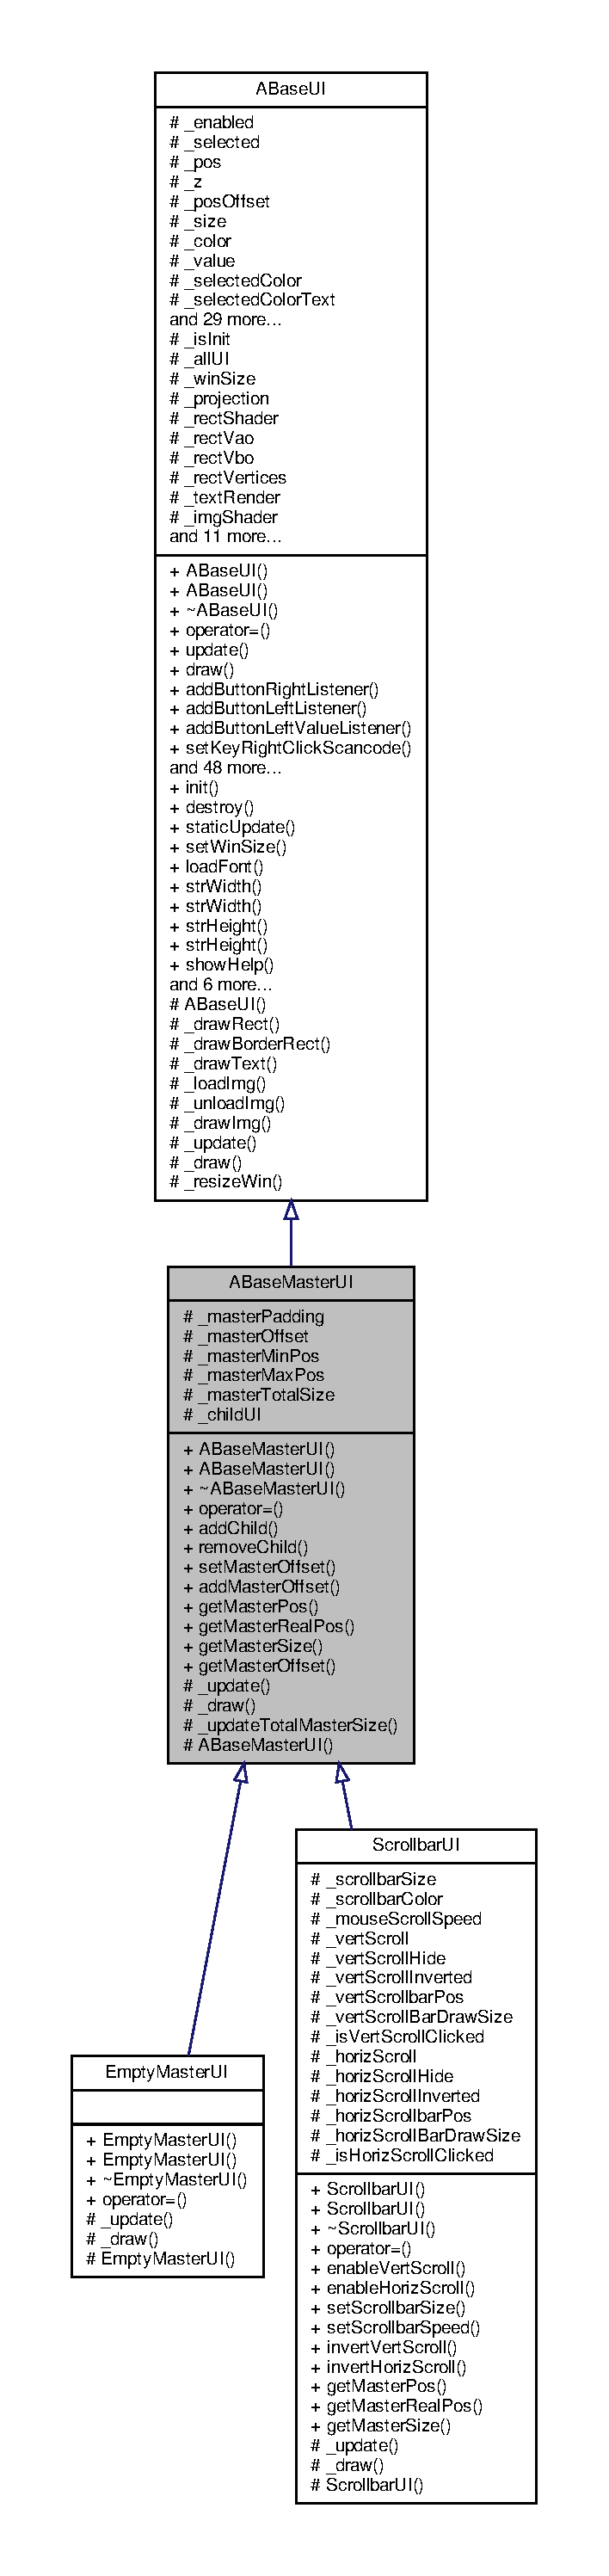
\includegraphics[height=550pt]{class_a_base_master_u_i__inherit__graph}
\end{center}
\end{figure}


Collaboration diagram for A\+Base\+Master\+UI\+:
\nopagebreak
\begin{figure}[H]
\begin{center}
\leavevmode
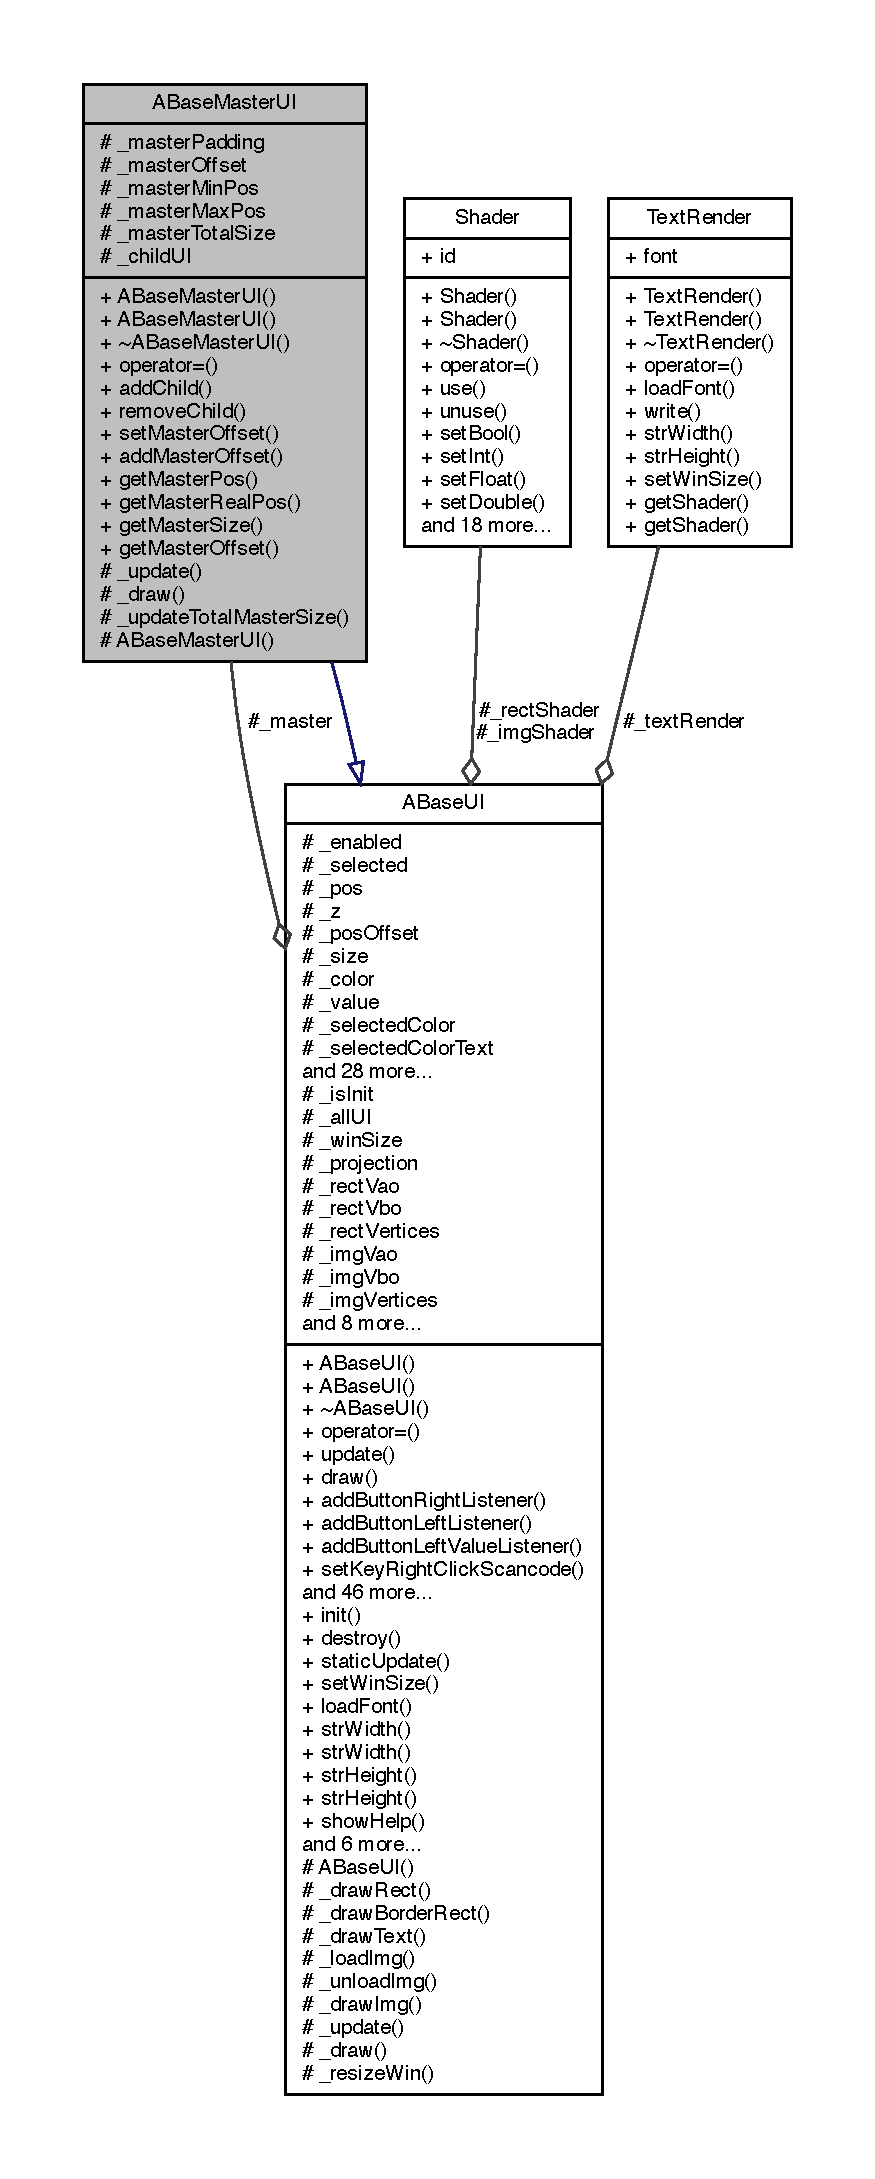
\includegraphics[height=550pt]{class_a_base_master_u_i__coll__graph}
\end{center}
\end{figure}
\doxysubsection*{Public Member Functions}
\begin{DoxyCompactItemize}
\item 
\mbox{\hyperlink{class_a_base_master_u_i_a311ce7af9ba882f3a274f6887c2196dc}{A\+Base\+Master\+UI}} (glm\+::vec2 pos, glm\+::vec2 size)
\begin{DoxyCompactList}\small\item\em Construct a new \mbox{\hyperlink{class_a_base_master_u_i_a311ce7af9ba882f3a274f6887c2196dc}{A\+Base\+Master\+U\+I\+::\+A\+Base\+Master\+UI}} object. \end{DoxyCompactList}\item 
\mbox{\hyperlink{class_a_base_master_u_i_aca816b5bc0624de287a3d386215a4c71}{A\+Base\+Master\+UI}} (\mbox{\hyperlink{class_a_base_master_u_i}{A\+Base\+Master\+UI}} const \&src)
\begin{DoxyCompactList}\small\item\em Construct a new \mbox{\hyperlink{class_a_base_master_u_i_a311ce7af9ba882f3a274f6887c2196dc}{A\+Base\+Master\+U\+I\+::\+A\+Base\+Master\+UI}} object. \end{DoxyCompactList}\item 
\mbox{\Hypertarget{class_a_base_master_u_i_a4714109951994c3f140add1f4effbcfb}\label{class_a_base_master_u_i_a4714109951994c3f140add1f4effbcfb}} 
virtual \mbox{\hyperlink{class_a_base_master_u_i_a4714109951994c3f140add1f4effbcfb}{$\sim$\+A\+Base\+Master\+UI}} ()
\begin{DoxyCompactList}\small\item\em Destroy the \mbox{\hyperlink{class_a_base_master_u_i_a311ce7af9ba882f3a274f6887c2196dc}{A\+Base\+Master\+U\+I\+::\+A\+Base\+Master\+UI}} object. \end{DoxyCompactList}\item 
\mbox{\hyperlink{class_a_base_master_u_i}{A\+Base\+Master\+UI}} \& \mbox{\hyperlink{class_a_base_master_u_i_a2023324b8f6cd85877c7932d5c46276f}{operator=}} (\mbox{\hyperlink{class_a_base_master_u_i}{A\+Base\+Master\+UI}} const \&rhs)
\begin{DoxyCompactList}\small\item\em Copy this object. \end{DoxyCompactList}\item 
void \mbox{\hyperlink{class_a_base_master_u_i_ae6bcaed259182e299cdfc6fabc8e01f1}{add\+Child}} (\mbox{\hyperlink{class_a_base_u_i}{A\+Base\+UI}} $\ast$child)
\begin{DoxyCompactList}\small\item\em Add a child in master element (called by set\+Master) \end{DoxyCompactList}\item 
void \mbox{\hyperlink{class_a_base_master_u_i_a0965153a5bf1d5a7de71f65c2f8fcc0a}{remove\+Child}} (\mbox{\hyperlink{class_a_base_u_i}{A\+Base\+UI}} $\ast$child)
\begin{DoxyCompactList}\small\item\em Remove a child in master element (called by set\+Master) \end{DoxyCompactList}\item 
void \mbox{\hyperlink{class_a_base_master_u_i_ad98439ff88bce6f13311f17444aea6f3}{set\+Master\+Offset}} (glm\+::vec2 offset)
\begin{DoxyCompactList}\small\item\em Set the offset of the master element. \end{DoxyCompactList}\item 
void \mbox{\hyperlink{class_a_base_master_u_i_a384c412cf0c2fc3265d9dc6bcb7ff57e}{add\+Master\+Offset}} (glm\+::vec2 offset)
\begin{DoxyCompactList}\small\item\em Add to the offset of the master element (last offset + new offset) \end{DoxyCompactList}\item 
virtual glm\+::vec2 \mbox{\hyperlink{class_a_base_master_u_i_aec1bb7871f82b2bd41de4fe4486e4050}{get\+Master\+Pos}} () const
\begin{DoxyCompactList}\small\item\em Get position of master element (bottom left after border) \end{DoxyCompactList}\item 
virtual glm\+::vec2 \mbox{\hyperlink{class_a_base_master_u_i_a64cf45d76b377fd59ec19f1f1d53c0be}{get\+Master\+Real\+Pos}} () const
\begin{DoxyCompactList}\small\item\em Get position of master element (bottom left after border) considering offset. \end{DoxyCompactList}\item 
virtual glm\+::vec2 \mbox{\hyperlink{class_a_base_master_u_i_ad8e2ca2b3f67ca274e5dd0169e454e55}{get\+Master\+Size}} () const
\begin{DoxyCompactList}\small\item\em Get size of master element inside the borders. \end{DoxyCompactList}\item 
virtual glm\+::vec2 \mbox{\hyperlink{class_a_base_master_u_i_aeeea67741ab77e3d03c6a817fc3bb949}{get\+Master\+Offset}} () const
\begin{DoxyCompactList}\small\item\em Get the master offset. \end{DoxyCompactList}\end{DoxyCompactItemize}
\doxysubsection*{Protected Member Functions}
\begin{DoxyCompactItemize}
\item 
virtual void \mbox{\hyperlink{class_a_base_master_u_i_a6c18f89d96c65d68ee1eabd8d4e1ee19}{\+\_\+update}} ()=0
\begin{DoxyCompactList}\small\item\em Update object. Called on every frames. \end{DoxyCompactList}\item 
virtual void \mbox{\hyperlink{class_a_base_master_u_i_ae92346a217da747e894a8acbe39b4397}{\+\_\+draw}} ()=0
\begin{DoxyCompactList}\small\item\em Draw object. Called on every frames. \end{DoxyCompactList}\item 
void \mbox{\hyperlink{class_a_base_master_u_i_a2bb6ad21838a1a2e1ce0bf7fb24a3330}{\+\_\+update\+Total\+Master\+Size}} ()
\begin{DoxyCompactList}\small\item\em Get the total size of all element in master. \end{DoxyCompactList}\end{DoxyCompactItemize}
\doxysubsection*{Protected Attributes}
\begin{DoxyCompactItemize}
\item 
glm\+::vec2 \mbox{\hyperlink{class_a_base_master_u_i_a381f24b69a5c92d1363fa855ed972e76}{\+\_\+master\+Padding}}
\item 
glm\+::vec2 \mbox{\hyperlink{class_a_base_master_u_i_a1f41b39f793a657af383ca420ca2a39b}{\+\_\+master\+Offset}}
\item 
glm\+::vec2 \mbox{\hyperlink{class_a_base_master_u_i_a9d907edd4ba081a74108846d1921908a}{\+\_\+master\+Min\+Pos}}
\item 
glm\+::vec2 \mbox{\hyperlink{class_a_base_master_u_i_a2a882142b0df3f748eef03dad099fc9c}{\+\_\+master\+Max\+Pos}}
\item 
glm\+::vec2 \mbox{\hyperlink{class_a_base_master_u_i_a1f2c4794773a4a3dcc00bd2871756898}{\+\_\+master\+Total\+Size}}
\item 
std\+::vector$<$ \mbox{\hyperlink{class_a_base_u_i}{A\+Base\+UI}} $\ast$ $>$ \mbox{\hyperlink{class_a_base_master_u_i_a8e67f5e6780889a29464f301f8d53e9a}{\+\_\+child\+UI}}
\end{DoxyCompactItemize}
\doxysubsection*{Additional Inherited Members}


\doxysubsection{Detailed Description}
this is the UI for all master objects 

Master objects are objects that contains others objects (for example the scrollbar is a master object) 

\doxysubsection{Constructor \& Destructor Documentation}
\mbox{\Hypertarget{class_a_base_master_u_i_a311ce7af9ba882f3a274f6887c2196dc}\label{class_a_base_master_u_i_a311ce7af9ba882f3a274f6887c2196dc}} 
\index{ABaseMasterUI@{ABaseMasterUI}!ABaseMasterUI@{ABaseMasterUI}}
\index{ABaseMasterUI@{ABaseMasterUI}!ABaseMasterUI@{ABaseMasterUI}}
\doxysubsubsection{\texorpdfstring{ABaseMasterUI()}{ABaseMasterUI()}\hspace{0.1cm}{\footnotesize\ttfamily [1/2]}}
{\footnotesize\ttfamily A\+Base\+Master\+U\+I\+::\+A\+Base\+Master\+UI (\begin{DoxyParamCaption}\item[{glm\+::vec2}]{pos,  }\item[{glm\+::vec2}]{size }\end{DoxyParamCaption})}



Construct a new \mbox{\hyperlink{class_a_base_master_u_i_a311ce7af9ba882f3a274f6887c2196dc}{A\+Base\+Master\+U\+I\+::\+A\+Base\+Master\+UI}} object. 


\begin{DoxyParams}{Parameters}
{\em pos} & The position of the UI element \\
\hline
{\em size} & The size of the UI element \\
\hline
\end{DoxyParams}
\mbox{\Hypertarget{class_a_base_master_u_i_aca816b5bc0624de287a3d386215a4c71}\label{class_a_base_master_u_i_aca816b5bc0624de287a3d386215a4c71}} 
\index{ABaseMasterUI@{ABaseMasterUI}!ABaseMasterUI@{ABaseMasterUI}}
\index{ABaseMasterUI@{ABaseMasterUI}!ABaseMasterUI@{ABaseMasterUI}}
\doxysubsubsection{\texorpdfstring{ABaseMasterUI()}{ABaseMasterUI()}\hspace{0.1cm}{\footnotesize\ttfamily [2/2]}}
{\footnotesize\ttfamily A\+Base\+Master\+U\+I\+::\+A\+Base\+Master\+UI (\begin{DoxyParamCaption}\item[{\mbox{\hyperlink{class_a_base_master_u_i}{A\+Base\+Master\+UI}} const \&}]{src }\end{DoxyParamCaption})}



Construct a new \mbox{\hyperlink{class_a_base_master_u_i_a311ce7af9ba882f3a274f6887c2196dc}{A\+Base\+Master\+U\+I\+::\+A\+Base\+Master\+UI}} object. 


\begin{DoxyParams}{Parameters}
{\em src} & The object to do the copy \\
\hline
\end{DoxyParams}


\doxysubsection{Member Function Documentation}
\mbox{\Hypertarget{class_a_base_master_u_i_ae92346a217da747e894a8acbe39b4397}\label{class_a_base_master_u_i_ae92346a217da747e894a8acbe39b4397}} 
\index{ABaseMasterUI@{ABaseMasterUI}!\_draw@{\_draw}}
\index{\_draw@{\_draw}!ABaseMasterUI@{ABaseMasterUI}}
\doxysubsubsection{\texorpdfstring{\_draw()}{\_draw()}}
{\footnotesize\ttfamily virtual void A\+Base\+Master\+U\+I\+::\+\_\+draw (\begin{DoxyParamCaption}{ }\end{DoxyParamCaption})\hspace{0.3cm}{\ttfamily [protected]}, {\ttfamily [pure virtual]}}



Draw object. Called on every frames. 

\begin{DoxyReturn}{Returns}
false If failed 
\end{DoxyReturn}


Implements \mbox{\hyperlink{class_a_base_u_i_a3331159cbf9926557afa79e4e3eee256}{A\+Base\+UI}}.



Implemented in \mbox{\hyperlink{class_scrollbar_u_i_adac2d8cc8f17d8db4170abe7ff9d3dad}{Scrollbar\+UI}}, and \mbox{\hyperlink{class_empty_master_u_i_a1e2b7cba4b43e28713c7e5d34a80b3a7}{Empty\+Master\+UI}}.

\mbox{\Hypertarget{class_a_base_master_u_i_a6c18f89d96c65d68ee1eabd8d4e1ee19}\label{class_a_base_master_u_i_a6c18f89d96c65d68ee1eabd8d4e1ee19}} 
\index{ABaseMasterUI@{ABaseMasterUI}!\_update@{\_update}}
\index{\_update@{\_update}!ABaseMasterUI@{ABaseMasterUI}}
\doxysubsubsection{\texorpdfstring{\_update()}{\_update()}}
{\footnotesize\ttfamily virtual void A\+Base\+Master\+U\+I\+::\+\_\+update (\begin{DoxyParamCaption}{ }\end{DoxyParamCaption})\hspace{0.3cm}{\ttfamily [protected]}, {\ttfamily [pure virtual]}}



Update object. Called on every frames. 

\begin{DoxyReturn}{Returns}
false If failed 
\end{DoxyReturn}


Implements \mbox{\hyperlink{class_a_base_u_i_ad4526888fd6a37de4086ba2a1e362759}{A\+Base\+UI}}.



Implemented in \mbox{\hyperlink{class_scrollbar_u_i_a75d909bc72204564034629439f6c0489}{Scrollbar\+UI}}, and \mbox{\hyperlink{class_empty_master_u_i_a1bf9ef11a2fa21e5637939ec6c959010}{Empty\+Master\+UI}}.

\mbox{\Hypertarget{class_a_base_master_u_i_a2bb6ad21838a1a2e1ce0bf7fb24a3330}\label{class_a_base_master_u_i_a2bb6ad21838a1a2e1ce0bf7fb24a3330}} 
\index{ABaseMasterUI@{ABaseMasterUI}!\_updateTotalMasterSize@{\_updateTotalMasterSize}}
\index{\_updateTotalMasterSize@{\_updateTotalMasterSize}!ABaseMasterUI@{ABaseMasterUI}}
\doxysubsubsection{\texorpdfstring{\_updateTotalMasterSize()}{\_updateTotalMasterSize()}}
{\footnotesize\ttfamily void A\+Base\+Master\+U\+I\+::\+\_\+update\+Total\+Master\+Size (\begin{DoxyParamCaption}{ }\end{DoxyParamCaption})\hspace{0.3cm}{\ttfamily [protected]}}



Get the total size of all element in master. 

this function update\+:
\begin{DoxyItemize}
\item \+\_\+master\+Min\+Pos\+: The minimum object position in object
\item \+\_\+master\+Max\+Pos\+: The maximum object position in object
\item \+\_\+master\+Total\+Size\+: The total size of master elements 
\end{DoxyItemize}\mbox{\Hypertarget{class_a_base_master_u_i_ae6bcaed259182e299cdfc6fabc8e01f1}\label{class_a_base_master_u_i_ae6bcaed259182e299cdfc6fabc8e01f1}} 
\index{ABaseMasterUI@{ABaseMasterUI}!addChild@{addChild}}
\index{addChild@{addChild}!ABaseMasterUI@{ABaseMasterUI}}
\doxysubsubsection{\texorpdfstring{addChild()}{addChild()}}
{\footnotesize\ttfamily void A\+Base\+Master\+U\+I\+::add\+Child (\begin{DoxyParamCaption}\item[{\mbox{\hyperlink{class_a_base_u_i}{A\+Base\+UI}} $\ast$}]{child }\end{DoxyParamCaption})}



Add a child in master element (called by set\+Master) 


\begin{DoxyParams}{Parameters}
{\em child} & The child element \\
\hline
\end{DoxyParams}
\mbox{\Hypertarget{class_a_base_master_u_i_a384c412cf0c2fc3265d9dc6bcb7ff57e}\label{class_a_base_master_u_i_a384c412cf0c2fc3265d9dc6bcb7ff57e}} 
\index{ABaseMasterUI@{ABaseMasterUI}!addMasterOffset@{addMasterOffset}}
\index{addMasterOffset@{addMasterOffset}!ABaseMasterUI@{ABaseMasterUI}}
\doxysubsubsection{\texorpdfstring{addMasterOffset()}{addMasterOffset()}}
{\footnotesize\ttfamily void A\+Base\+Master\+U\+I\+::add\+Master\+Offset (\begin{DoxyParamCaption}\item[{glm\+::vec2}]{offset }\end{DoxyParamCaption})}



Add to the offset of the master element (last offset + new offset) 


\begin{DoxyParams}{Parameters}
{\em offset} & The offset adder \\
\hline
\end{DoxyParams}
\mbox{\Hypertarget{class_a_base_master_u_i_aeeea67741ab77e3d03c6a817fc3bb949}\label{class_a_base_master_u_i_aeeea67741ab77e3d03c6a817fc3bb949}} 
\index{ABaseMasterUI@{ABaseMasterUI}!getMasterOffset@{getMasterOffset}}
\index{getMasterOffset@{getMasterOffset}!ABaseMasterUI@{ABaseMasterUI}}
\doxysubsubsection{\texorpdfstring{getMasterOffset()}{getMasterOffset()}}
{\footnotesize\ttfamily glm\+::vec2 A\+Base\+Master\+U\+I\+::get\+Master\+Offset (\begin{DoxyParamCaption}{ }\end{DoxyParamCaption}) const\hspace{0.3cm}{\ttfamily [virtual]}}



Get the master offset. 

\begin{DoxyReturn}{Returns}
glm\+::vec2 The offset 
\end{DoxyReturn}
\mbox{\Hypertarget{class_a_base_master_u_i_aec1bb7871f82b2bd41de4fe4486e4050}\label{class_a_base_master_u_i_aec1bb7871f82b2bd41de4fe4486e4050}} 
\index{ABaseMasterUI@{ABaseMasterUI}!getMasterPos@{getMasterPos}}
\index{getMasterPos@{getMasterPos}!ABaseMasterUI@{ABaseMasterUI}}
\doxysubsubsection{\texorpdfstring{getMasterPos()}{getMasterPos()}}
{\footnotesize\ttfamily glm\+::vec2 A\+Base\+Master\+U\+I\+::get\+Master\+Pos (\begin{DoxyParamCaption}{ }\end{DoxyParamCaption}) const\hspace{0.3cm}{\ttfamily [virtual]}}



Get position of master element (bottom left after border) 

!!! This functions can be overwrite in childs class

\begin{DoxyReturn}{Returns}
glm\+::vec2 The position 
\end{DoxyReturn}


Reimplemented in \mbox{\hyperlink{class_scrollbar_u_i_a3a4c39a263f6bf7783b1054f57a26ee7}{Scrollbar\+UI}}.

\mbox{\Hypertarget{class_a_base_master_u_i_a64cf45d76b377fd59ec19f1f1d53c0be}\label{class_a_base_master_u_i_a64cf45d76b377fd59ec19f1f1d53c0be}} 
\index{ABaseMasterUI@{ABaseMasterUI}!getMasterRealPos@{getMasterRealPos}}
\index{getMasterRealPos@{getMasterRealPos}!ABaseMasterUI@{ABaseMasterUI}}
\doxysubsubsection{\texorpdfstring{getMasterRealPos()}{getMasterRealPos()}}
{\footnotesize\ttfamily glm\+::vec2 A\+Base\+Master\+U\+I\+::get\+Master\+Real\+Pos (\begin{DoxyParamCaption}{ }\end{DoxyParamCaption}) const\hspace{0.3cm}{\ttfamily [virtual]}}



Get position of master element (bottom left after border) considering offset. 

!!! This functions can be overwrite in childs class

\begin{DoxyReturn}{Returns}
glm\+::vec2 The position 
\end{DoxyReturn}


Reimplemented in \mbox{\hyperlink{class_scrollbar_u_i_a7dd8afe939f8b8a5f9486eeec1f56d92}{Scrollbar\+UI}}.

\mbox{\Hypertarget{class_a_base_master_u_i_ad8e2ca2b3f67ca274e5dd0169e454e55}\label{class_a_base_master_u_i_ad8e2ca2b3f67ca274e5dd0169e454e55}} 
\index{ABaseMasterUI@{ABaseMasterUI}!getMasterSize@{getMasterSize}}
\index{getMasterSize@{getMasterSize}!ABaseMasterUI@{ABaseMasterUI}}
\doxysubsubsection{\texorpdfstring{getMasterSize()}{getMasterSize()}}
{\footnotesize\ttfamily glm\+::vec2 A\+Base\+Master\+U\+I\+::get\+Master\+Size (\begin{DoxyParamCaption}{ }\end{DoxyParamCaption}) const\hspace{0.3cm}{\ttfamily [virtual]}}



Get size of master element inside the borders. 

!!! This functions can be overwrite in childs class

\begin{DoxyReturn}{Returns}
glm\+::vec2 The size 
\end{DoxyReturn}


Reimplemented in \mbox{\hyperlink{class_scrollbar_u_i_ad9f2de5f7fbb4acdfe25fc2dbe3eb943}{Scrollbar\+UI}}.

\mbox{\Hypertarget{class_a_base_master_u_i_a2023324b8f6cd85877c7932d5c46276f}\label{class_a_base_master_u_i_a2023324b8f6cd85877c7932d5c46276f}} 
\index{ABaseMasterUI@{ABaseMasterUI}!operator=@{operator=}}
\index{operator=@{operator=}!ABaseMasterUI@{ABaseMasterUI}}
\doxysubsubsection{\texorpdfstring{operator=()}{operator=()}}
{\footnotesize\ttfamily \mbox{\hyperlink{class_a_base_master_u_i}{A\+Base\+Master\+UI}} \& A\+Base\+Master\+U\+I\+::operator= (\begin{DoxyParamCaption}\item[{\mbox{\hyperlink{class_a_base_master_u_i}{A\+Base\+Master\+UI}} const \&}]{rhs }\end{DoxyParamCaption})}



Copy this object. 


\begin{DoxyParams}{Parameters}
{\em rhs} & The object to copy \\
\hline
\end{DoxyParams}
\begin{DoxyReturn}{Returns}
\mbox{\hyperlink{class_a_base_master_u_i}{A\+Base\+Master\+UI}}\& A reference to the copied object 
\end{DoxyReturn}
\mbox{\Hypertarget{class_a_base_master_u_i_a0965153a5bf1d5a7de71f65c2f8fcc0a}\label{class_a_base_master_u_i_a0965153a5bf1d5a7de71f65c2f8fcc0a}} 
\index{ABaseMasterUI@{ABaseMasterUI}!removeChild@{removeChild}}
\index{removeChild@{removeChild}!ABaseMasterUI@{ABaseMasterUI}}
\doxysubsubsection{\texorpdfstring{removeChild()}{removeChild()}}
{\footnotesize\ttfamily void A\+Base\+Master\+U\+I\+::remove\+Child (\begin{DoxyParamCaption}\item[{\mbox{\hyperlink{class_a_base_u_i}{A\+Base\+UI}} $\ast$}]{child }\end{DoxyParamCaption})}



Remove a child in master element (called by set\+Master) 


\begin{DoxyParams}{Parameters}
{\em child} & The child element \\
\hline
\end{DoxyParams}
\mbox{\Hypertarget{class_a_base_master_u_i_ad98439ff88bce6f13311f17444aea6f3}\label{class_a_base_master_u_i_ad98439ff88bce6f13311f17444aea6f3}} 
\index{ABaseMasterUI@{ABaseMasterUI}!setMasterOffset@{setMasterOffset}}
\index{setMasterOffset@{setMasterOffset}!ABaseMasterUI@{ABaseMasterUI}}
\doxysubsubsection{\texorpdfstring{setMasterOffset()}{setMasterOffset()}}
{\footnotesize\ttfamily void A\+Base\+Master\+U\+I\+::set\+Master\+Offset (\begin{DoxyParamCaption}\item[{glm\+::vec2}]{offset }\end{DoxyParamCaption})}



Set the offset of the master element. 


\begin{DoxyParams}{Parameters}
{\em offset} & The new offset \\
\hline
\end{DoxyParams}


\doxysubsection{Member Data Documentation}
\mbox{\Hypertarget{class_a_base_master_u_i_a8e67f5e6780889a29464f301f8d53e9a}\label{class_a_base_master_u_i_a8e67f5e6780889a29464f301f8d53e9a}} 
\index{ABaseMasterUI@{ABaseMasterUI}!\_childUI@{\_childUI}}
\index{\_childUI@{\_childUI}!ABaseMasterUI@{ABaseMasterUI}}
\doxysubsubsection{\texorpdfstring{\_childUI}{\_childUI}}
{\footnotesize\ttfamily std\+::vector$<$\mbox{\hyperlink{class_a_base_u_i}{A\+Base\+UI}} $\ast$$>$ A\+Base\+Master\+U\+I\+::\+\_\+child\+UI\hspace{0.3cm}{\ttfamily [protected]}}

All childs reference \mbox{\Hypertarget{class_a_base_master_u_i_a2a882142b0df3f748eef03dad099fc9c}\label{class_a_base_master_u_i_a2a882142b0df3f748eef03dad099fc9c}} 
\index{ABaseMasterUI@{ABaseMasterUI}!\_masterMaxPos@{\_masterMaxPos}}
\index{\_masterMaxPos@{\_masterMaxPos}!ABaseMasterUI@{ABaseMasterUI}}
\doxysubsubsection{\texorpdfstring{\_masterMaxPos}{\_masterMaxPos}}
{\footnotesize\ttfamily glm\+::vec2 A\+Base\+Master\+U\+I\+::\+\_\+master\+Max\+Pos\hspace{0.3cm}{\ttfamily [protected]}}

Bottom position \mbox{\Hypertarget{class_a_base_master_u_i_a9d907edd4ba081a74108846d1921908a}\label{class_a_base_master_u_i_a9d907edd4ba081a74108846d1921908a}} 
\index{ABaseMasterUI@{ABaseMasterUI}!\_masterMinPos@{\_masterMinPos}}
\index{\_masterMinPos@{\_masterMinPos}!ABaseMasterUI@{ABaseMasterUI}}
\doxysubsubsection{\texorpdfstring{\_masterMinPos}{\_masterMinPos}}
{\footnotesize\ttfamily glm\+::vec2 A\+Base\+Master\+U\+I\+::\+\_\+master\+Min\+Pos\hspace{0.3cm}{\ttfamily [protected]}}

Top position \mbox{\Hypertarget{class_a_base_master_u_i_a1f41b39f793a657af383ca420ca2a39b}\label{class_a_base_master_u_i_a1f41b39f793a657af383ca420ca2a39b}} 
\index{ABaseMasterUI@{ABaseMasterUI}!\_masterOffset@{\_masterOffset}}
\index{\_masterOffset@{\_masterOffset}!ABaseMasterUI@{ABaseMasterUI}}
\doxysubsubsection{\texorpdfstring{\_masterOffset}{\_masterOffset}}
{\footnotesize\ttfamily glm\+::vec2 A\+Base\+Master\+U\+I\+::\+\_\+master\+Offset\hspace{0.3cm}{\ttfamily [protected]}}

Master offset (used to move childs objects) \mbox{\Hypertarget{class_a_base_master_u_i_a381f24b69a5c92d1363fa855ed972e76}\label{class_a_base_master_u_i_a381f24b69a5c92d1363fa855ed972e76}} 
\index{ABaseMasterUI@{ABaseMasterUI}!\_masterPadding@{\_masterPadding}}
\index{\_masterPadding@{\_masterPadding}!ABaseMasterUI@{ABaseMasterUI}}
\doxysubsubsection{\texorpdfstring{\_masterPadding}{\_masterPadding}}
{\footnotesize\ttfamily glm\+::vec2 A\+Base\+Master\+U\+I\+::\+\_\+master\+Padding\hspace{0.3cm}{\ttfamily [protected]}}

Master padding \mbox{\Hypertarget{class_a_base_master_u_i_a1f2c4794773a4a3dcc00bd2871756898}\label{class_a_base_master_u_i_a1f2c4794773a4a3dcc00bd2871756898}} 
\index{ABaseMasterUI@{ABaseMasterUI}!\_masterTotalSize@{\_masterTotalSize}}
\index{\_masterTotalSize@{\_masterTotalSize}!ABaseMasterUI@{ABaseMasterUI}}
\doxysubsubsection{\texorpdfstring{\_masterTotalSize}{\_masterTotalSize}}
{\footnotesize\ttfamily glm\+::vec2 A\+Base\+Master\+U\+I\+::\+\_\+master\+Total\+Size\hspace{0.3cm}{\ttfamily [protected]}}

Total size (size \& pos of all childs) 

The documentation for this class was generated from the following files\+:\begin{DoxyCompactItemize}
\item 
includes/utils/opengl/\+U\+I/A\+Base\+Master\+U\+I.\+hpp\item 
srcs/utils/opengl/\+U\+I/A\+Base\+Master\+U\+I.\+cpp\end{DoxyCompactItemize}

\hypertarget{class_a_base_u_i}{}\doxysection{A\+Base\+UI Class Reference}
\label{class_a_base_u_i}\index{ABaseUI@{ABaseUI}}


this is the base UI interface  




{\ttfamily \#include $<$A\+Base\+U\+I.\+hpp$>$}



Inheritance diagram for A\+Base\+UI\+:
\nopagebreak
\begin{figure}[H]
\begin{center}
\leavevmode
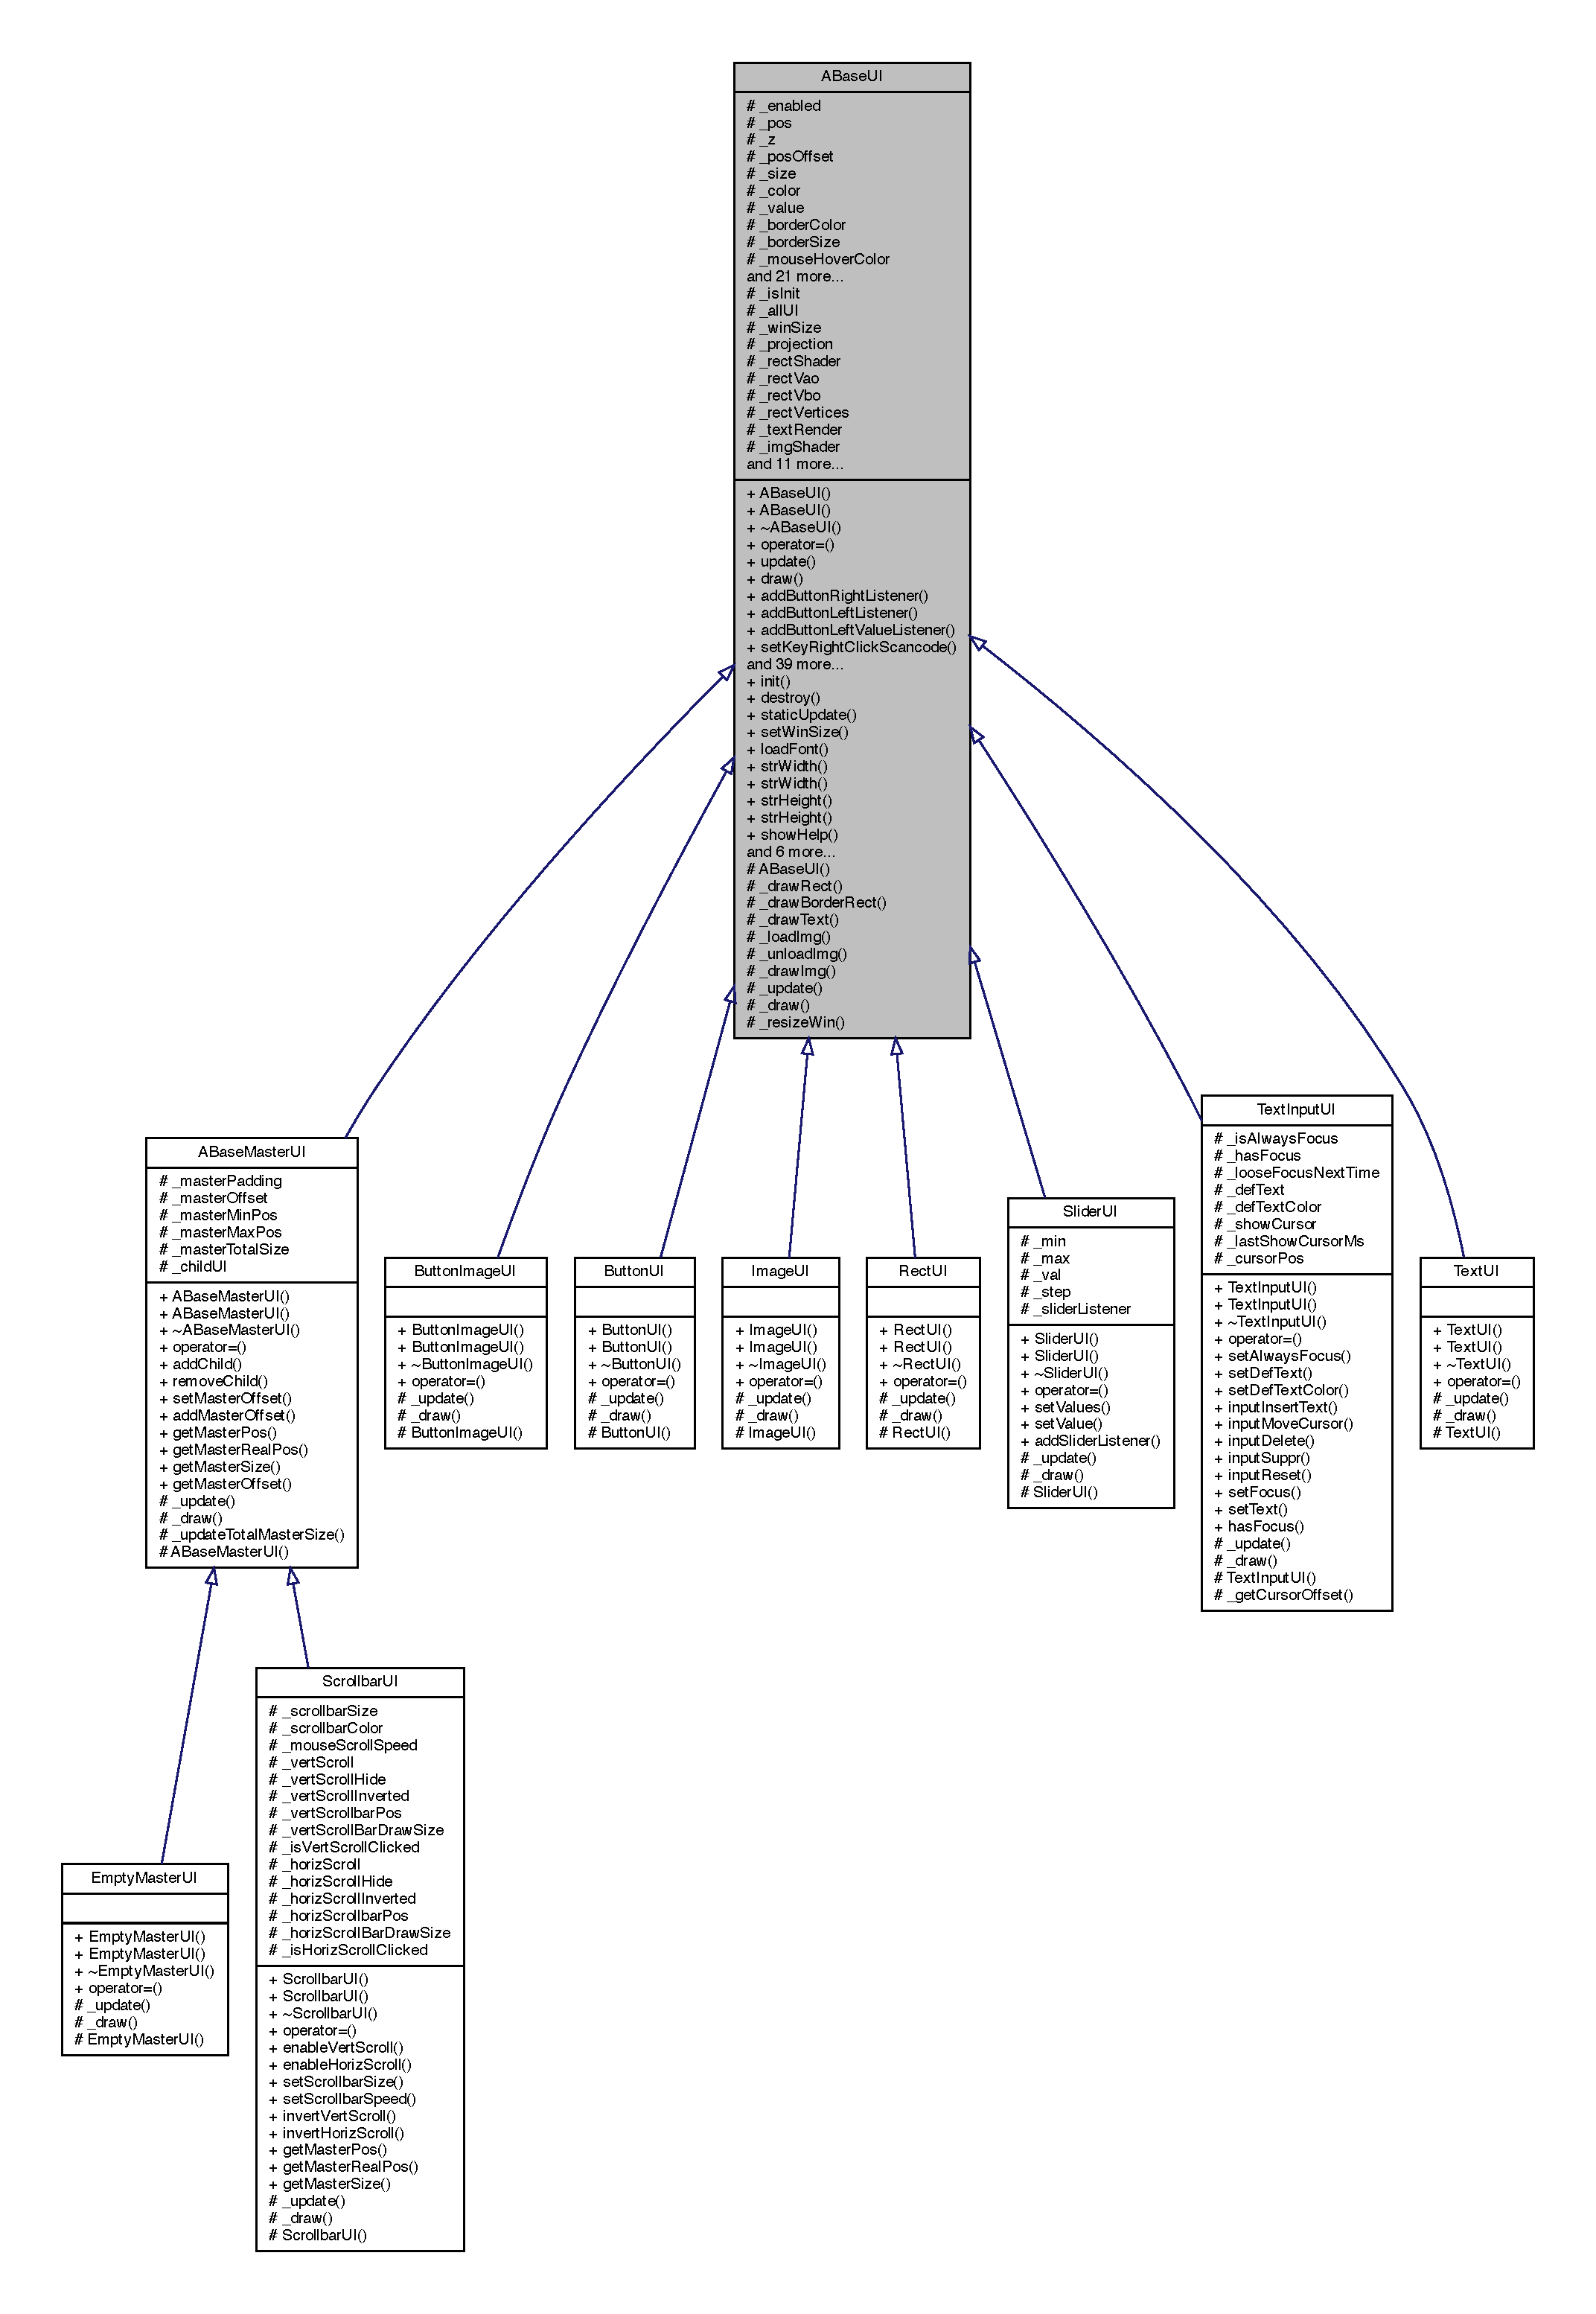
\includegraphics[width=350pt]{class_a_base_u_i__inherit__graph}
\end{center}
\end{figure}


Collaboration diagram for A\+Base\+UI\+:
\nopagebreak
\begin{figure}[H]
\begin{center}
\leavevmode
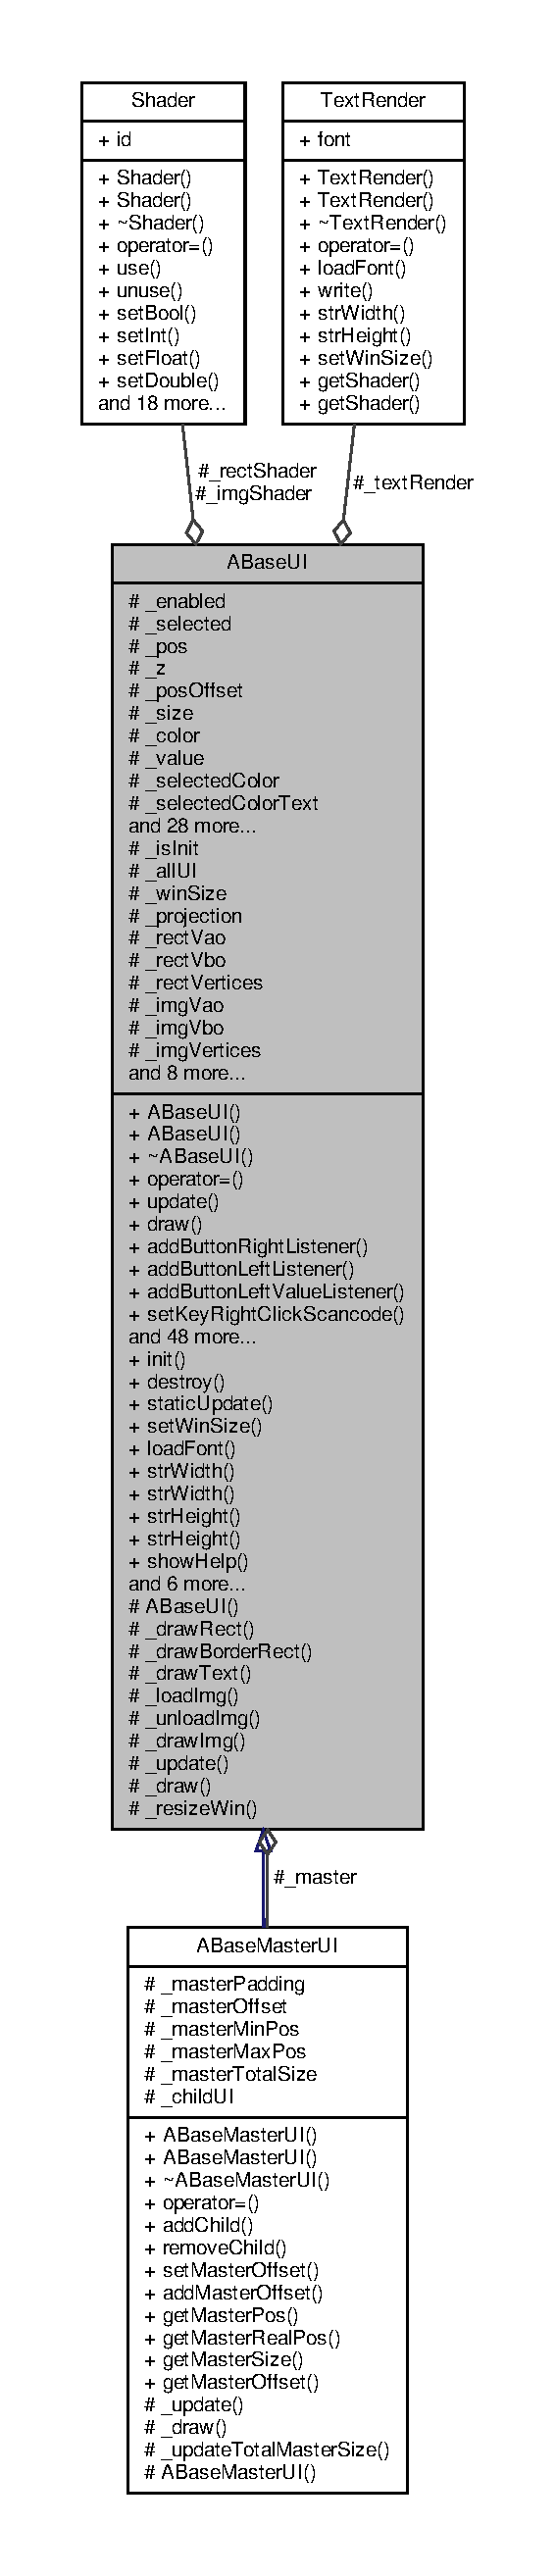
\includegraphics[height=550pt]{class_a_base_u_i__coll__graph}
\end{center}
\end{figure}
\doxysubsection*{Classes}
\begin{DoxyCompactItemize}
\item 
class \mbox{\hyperlink{class_a_base_u_i_1_1_u_i_exception}{U\+I\+Exception}}
\begin{DoxyCompactList}\small\item\em UI exception. \end{DoxyCompactList}\end{DoxyCompactItemize}
\doxysubsection*{Public Member Functions}
\begin{DoxyCompactItemize}
\item 
\mbox{\hyperlink{class_a_base_u_i_a643d80d189018a179d2e3a938e3aa539}{A\+Base\+UI}} (glm\+::vec2 pos, glm\+::vec2 size)
\begin{DoxyCompactList}\small\item\em Construct a new \mbox{\hyperlink{class_a_base_u_i_a643d80d189018a179d2e3a938e3aa539}{A\+Base\+U\+I\+::\+A\+Base\+UI}} object. \end{DoxyCompactList}\item 
\mbox{\hyperlink{class_a_base_u_i_a43914df26b12e74becb41da8d85448f1}{A\+Base\+UI}} (\mbox{\hyperlink{class_a_base_u_i}{A\+Base\+UI}} const \&src)
\begin{DoxyCompactList}\small\item\em Construct a new \mbox{\hyperlink{class_a_base_u_i_a643d80d189018a179d2e3a938e3aa539}{A\+Base\+U\+I\+::\+A\+Base\+UI}} object. \end{DoxyCompactList}\item 
\mbox{\Hypertarget{class_a_base_u_i_ac2fd1305e127a9c547c37dd58f65742d}\label{class_a_base_u_i_ac2fd1305e127a9c547c37dd58f65742d}} 
virtual \mbox{\hyperlink{class_a_base_u_i_ac2fd1305e127a9c547c37dd58f65742d}{$\sim$\+A\+Base\+UI}} ()
\begin{DoxyCompactList}\small\item\em Destroy the \mbox{\hyperlink{class_a_base_u_i_a643d80d189018a179d2e3a938e3aa539}{A\+Base\+U\+I\+::\+A\+Base\+UI}} object. \end{DoxyCompactList}\item 
\mbox{\hyperlink{class_a_base_u_i}{A\+Base\+UI}} \& \mbox{\hyperlink{class_a_base_u_i_af269cad7ae1f290964cdeeb3f84cdc89}{operator=}} (\mbox{\hyperlink{class_a_base_u_i}{A\+Base\+UI}} const \&rhs)
\begin{DoxyCompactList}\small\item\em Copy this object. \end{DoxyCompactList}\item 
\mbox{\Hypertarget{class_a_base_u_i_aa191d2729152b1b381cb4eba7d2b178e}\label{class_a_base_u_i_aa191d2729152b1b381cb4eba7d2b178e}} 
void \mbox{\hyperlink{class_a_base_u_i_aa191d2729152b1b381cb4eba7d2b178e}{update}} ()
\begin{DoxyCompactList}\small\item\em This is the base update function of UI objects. \end{DoxyCompactList}\item 
\mbox{\Hypertarget{class_a_base_u_i_ab8be8a69c8d5db4727921869dc942c7f}\label{class_a_base_u_i_ab8be8a69c8d5db4727921869dc942c7f}} 
void \mbox{\hyperlink{class_a_base_u_i_ab8be8a69c8d5db4727921869dc942c7f}{draw}} ()
\begin{DoxyCompactList}\small\item\em This is the base draw function of UI objects. \end{DoxyCompactList}\item 
virtual \mbox{\hyperlink{class_a_base_u_i}{A\+Base\+UI}} \& \mbox{\hyperlink{class_a_base_u_i_a63ab2419d2aa942726854770a54ca15f}{add\+Button\+Right\+Listener}} (bool $\ast$listener)
\begin{DoxyCompactList}\small\item\em add a listener on the right click \end{DoxyCompactList}\item 
virtual \mbox{\hyperlink{class_a_base_u_i}{A\+Base\+UI}} \& \mbox{\hyperlink{class_a_base_u_i_a99d5577cc79031a9711196bf4f583a91}{add\+Button\+Left\+Listener}} (bool $\ast$listener)
\begin{DoxyCompactList}\small\item\em add a listener on the left click \end{DoxyCompactList}\item 
virtual \mbox{\hyperlink{class_a_base_u_i}{A\+Base\+UI}} \& \mbox{\hyperlink{class_a_base_u_i_a9d351ded131d2d5ef546616a166ace59}{add\+Button\+Left\+Value\+Listener}} (int64\+\_\+t $\ast$listener, int64\+\_\+t value)
\begin{DoxyCompactList}\small\item\em add a listener on the left click who will be modify to value \end{DoxyCompactList}\item 
virtual \mbox{\hyperlink{class_a_base_u_i}{A\+Base\+UI}} \& \mbox{\hyperlink{class_a_base_u_i_a2929b4cb63c16464efa957038d523c02}{set\+Key\+Right\+Click\+Scancode}} (S\+D\+L\+\_\+\+Scancode scancode)
\begin{DoxyCompactList}\small\item\em Set the right click shortcut. \end{DoxyCompactList}\item 
virtual \mbox{\hyperlink{class_a_base_u_i}{A\+Base\+UI}} \& \mbox{\hyperlink{class_a_base_u_i_aba668d6b9c8bf7e1e0b94dfb0b6aaab1}{set\+Key\+Left\+Click\+Scancode}} (S\+D\+L\+\_\+\+Scancode scancode)
\begin{DoxyCompactList}\small\item\em Set the left click shortcut. \end{DoxyCompactList}\item 
virtual \mbox{\hyperlink{class_a_base_u_i}{A\+Base\+UI}} \& \mbox{\hyperlink{class_a_base_u_i_a28c110e7ad0f77043d5348035bd39f7a}{set\+Key\+Right\+Click\+Input}} (Input\+Type\+::\+Enum input)
\begin{DoxyCompactList}\small\item\em Set the right click shortcut. \end{DoxyCompactList}\item 
virtual \mbox{\hyperlink{class_a_base_u_i}{A\+Base\+UI}} \& \mbox{\hyperlink{class_a_base_u_i_a2a2b600c735d45f2ea2c14291a5292ba}{set\+Key\+Left\+Click\+Input}} (Input\+Type\+::\+Enum input)
\begin{DoxyCompactList}\small\item\em Set the left click shortcut. \end{DoxyCompactList}\item 
virtual \mbox{\hyperlink{class_a_base_u_i}{A\+Base\+UI}} \& \mbox{\hyperlink{class_a_base_u_i_a9b19e675593c03f7d5becbd580bc418b}{set\+Enabled}} (bool enabled)
\begin{DoxyCompactList}\small\item\em Enable / disable UI. \end{DoxyCompactList}\item 
virtual \mbox{\hyperlink{class_a_base_u_i}{A\+Base\+UI}} \& \mbox{\hyperlink{class_a_base_u_i_abe931f9a44c29212a667cdd0f1da6365}{set\+Selected}} (bool selected)
\begin{DoxyCompactList}\small\item\em Selected / unselected UI. \end{DoxyCompactList}\item 
virtual \mbox{\hyperlink{class_a_base_u_i}{A\+Base\+UI}} \& \mbox{\hyperlink{class_a_base_u_i_a68ad426cc75f6a61fe000c8e92d4df0c}{set\+Pos}} (glm\+::vec2 pos)
\begin{DoxyCompactList}\small\item\em Set position. \end{DoxyCompactList}\item 
virtual \mbox{\hyperlink{class_a_base_u_i}{A\+Base\+UI}} \& \mbox{\hyperlink{class_a_base_u_i_a9b7e138cf37199808f55a4596efe4ac9}{setZ}} (float z)
\begin{DoxyCompactList}\small\item\em Set Z (used for transparency) \end{DoxyCompactList}\item 
virtual \mbox{\hyperlink{class_a_base_u_i}{A\+Base\+UI}} \& \mbox{\hyperlink{class_a_base_u_i_a6e209b2a871a2a4afa69f5dff2c6d89e}{set\+Pos\+Offset}} (glm\+::vec2 offset)
\begin{DoxyCompactList}\small\item\em Set position offset (to move object whitout change position) \end{DoxyCompactList}\item 
virtual \mbox{\hyperlink{class_a_base_u_i}{A\+Base\+UI}} \& \mbox{\hyperlink{class_a_base_u_i_abdf5aa14ea0b34192142fcbff0348fc0}{add\+Pos\+Offset}} (glm\+::vec2 offset)
\begin{DoxyCompactList}\small\item\em Add to position offset (to move object whitout change position) \end{DoxyCompactList}\item 
virtual \mbox{\hyperlink{class_a_base_u_i}{A\+Base\+UI}} \& \mbox{\hyperlink{class_a_base_u_i_ae50c31f566ad854411d09f75c2190c12}{set\+Size}} (glm\+::vec2 size)
\begin{DoxyCompactList}\small\item\em Set the object size. \end{DoxyCompactList}\item 
virtual \mbox{\hyperlink{class_a_base_u_i}{A\+Base\+UI}} \& \mbox{\hyperlink{class_a_base_u_i_aad292aed7bb28a2c8654ddfb54596a2c}{set\+Calculated\+Size}} ()
\begin{DoxyCompactList}\small\item\em Auto calculate size from the text size. \end{DoxyCompactList}\item 
virtual \mbox{\hyperlink{class_a_base_u_i}{A\+Base\+UI}} \& \mbox{\hyperlink{class_a_base_u_i_a13a7acc1e7ffa2c139c74e841d744753}{set\+Color}} (glm\+::vec4 color)
\begin{DoxyCompactList}\small\item\em Set the color. \end{DoxyCompactList}\item 
virtual \mbox{\hyperlink{class_a_base_u_i}{A\+Base\+UI}} \& \mbox{\hyperlink{class_a_base_u_i_a048cb78b3a5c32aa7ab844ffa445d7a5}{set\+Selected\+Color}} (glm\+::vec4 color)
\begin{DoxyCompactList}\small\item\em Set the color selected. \end{DoxyCompactList}\item 
virtual \mbox{\hyperlink{class_a_base_u_i}{A\+Base\+UI}} \& \mbox{\hyperlink{class_a_base_u_i_a5843ff5ba45830356043a6fefc24f798}{set\+Selected\+Color\+Text}} (glm\+::vec4 color)
\begin{DoxyCompactList}\small\item\em Set the color selected text. \end{DoxyCompactList}\item 
virtual \mbox{\hyperlink{class_a_base_u_i}{A\+Base\+UI}} \& \mbox{\hyperlink{class_a_base_u_i_a16d0d5da4f14b3e43a10f64cefbf8290}{set\+Border\+Color}} (glm\+::vec4 color)
\begin{DoxyCompactList}\small\item\em Set the border color. \end{DoxyCompactList}\item 
virtual \mbox{\hyperlink{class_a_base_u_i}{A\+Base\+UI}} \& \mbox{\hyperlink{class_a_base_u_i_a3028cb83474c9a384dac58d110aa196f}{set\+Border\+Size}} (float size)
\begin{DoxyCompactList}\small\item\em Set the border size. \end{DoxyCompactList}\item 
virtual \mbox{\hyperlink{class_a_base_u_i}{A\+Base\+UI}} \& \mbox{\hyperlink{class_a_base_u_i_a902c194cc52e03a49f52c74bdbe61deb}{set\+Mouse\+Hover\+Color}} (glm\+::vec4 color)
\begin{DoxyCompactList}\small\item\em Set the mouse hover color. \end{DoxyCompactList}\item 
virtual \mbox{\hyperlink{class_a_base_u_i}{A\+Base\+UI}} \& \mbox{\hyperlink{class_a_base_u_i_a27891d827140704a50a25f55c4939c03}{set\+Mouse\+Hover\+Color\+Text}} (glm\+::vec4 color)
\begin{DoxyCompactList}\small\item\em Set the mouse hover color text. \end{DoxyCompactList}\item 
virtual \mbox{\hyperlink{class_a_base_u_i}{A\+Base\+UI}} \& \mbox{\hyperlink{class_a_base_u_i_ab93705fee3e6dfdc900bea21a42695e0}{set\+Mouse\+Click\+Color}} (glm\+::vec4 color)
\begin{DoxyCompactList}\small\item\em Set the mouse click color. \end{DoxyCompactList}\item 
virtual \mbox{\hyperlink{class_a_base_u_i}{A\+Base\+UI}} \& \mbox{\hyperlink{class_a_base_u_i_a0afbe90ac3012028bd9895cdfe0d7861}{set\+Mouse\+Click\+Color\+Text}} (glm\+::vec4 color)
\begin{DoxyCompactList}\small\item\em Set the mouse click color text. \end{DoxyCompactList}\item 
virtual \mbox{\hyperlink{class_a_base_u_i}{A\+Base\+UI}} \& \mbox{\hyperlink{class_a_base_u_i_a82e182bfd577d37224aa49be3f64ac87}{set\+Text}} (std\+::string const \&text)
\begin{DoxyCompactList}\small\item\em Set the text. \end{DoxyCompactList}\item 
virtual \mbox{\hyperlink{class_a_base_u_i}{A\+Base\+UI}} \& \mbox{\hyperlink{class_a_base_u_i_a5d22d531f4fd1d59b9cfff0f2f3e4b8d}{set\+Text\+Color}} (glm\+::vec4 color)
\begin{DoxyCompactList}\small\item\em Set the text color. \end{DoxyCompactList}\item 
virtual \mbox{\hyperlink{class_a_base_u_i}{A\+Base\+UI}} \& \mbox{\hyperlink{class_a_base_u_i_a705188de51bf8387d38dca90740262a0}{set\+Text\+Font}} (std\+::string const \&font)
\begin{DoxyCompactList}\small\item\em Set the text font. \end{DoxyCompactList}\item 
virtual \mbox{\hyperlink{class_a_base_u_i}{A\+Base\+UI}} \& \mbox{\hyperlink{class_a_base_u_i_a980fa680f895fdefb7ee94ba022cd29b}{set\+Text\+Scale}} (float scale)
\begin{DoxyCompactList}\small\item\em Set the text scale. \end{DoxyCompactList}\item 
virtual \mbox{\hyperlink{class_a_base_u_i}{A\+Base\+UI}} \& \mbox{\hyperlink{class_a_base_u_i_ad414a59cf590b50f2d1f37891edf7284}{set\+Text\+Padding}} (float padding)
\begin{DoxyCompactList}\small\item\em Set the text padding. \end{DoxyCompactList}\item 
virtual \mbox{\hyperlink{class_a_base_u_i}{A\+Base\+UI}} \& \mbox{\hyperlink{class_a_base_u_i_a4a88d65cb4a5767c280e0849e56a519b}{set\+Text\+Align}} (Text\+Align\+::\+Enum align)
\begin{DoxyCompactList}\small\item\em Set the text alignment. \end{DoxyCompactList}\item 
virtual \mbox{\hyperlink{class_a_base_u_i}{A\+Base\+UI}} \& \mbox{\hyperlink{class_a_base_u_i_a1bafea512714350e238ef0cf0bd4e416}{set\+Text\+Outline}} (float outline)
\begin{DoxyCompactList}\small\item\em Set the text outline. \end{DoxyCompactList}\item 
virtual \mbox{\hyperlink{class_a_base_u_i}{A\+Base\+UI}} \& \mbox{\hyperlink{class_a_base_u_i_a5490ceb10f7b8184d11bd4cd32a6adeb}{set\+Text\+Outline\+Color}} (glm\+::vec4 color)
\begin{DoxyCompactList}\small\item\em Set the text outline color. \end{DoxyCompactList}\item 
virtual \mbox{\hyperlink{class_a_base_u_i}{A\+Base\+UI}} \& \mbox{\hyperlink{class_a_base_u_i_a258f301b41ab8cc9e1b50ca38c27ca78}{set\+Master}} (\mbox{\hyperlink{class_a_base_master_u_i}{A\+Base\+Master\+UI}} $\ast$master)
\begin{DoxyCompactList}\small\item\em Set the master object. \end{DoxyCompactList}\item 
virtual bool \mbox{\hyperlink{class_a_base_u_i_af83c894a28e16ae8c008da87a617e8fd}{is\+Partially\+Out\+Of\+Screen}} () const
\begin{DoxyCompactList}\small\item\em Check if the UI element is partially out of the screen. \end{DoxyCompactList}\item 
virtual bool \mbox{\hyperlink{class_a_base_u_i_a43ccdbcb5f1e7292cd013c2d1ba3704c}{is\+Totally\+Out\+Of\+Screen}} () const
\begin{DoxyCompactList}\small\item\em Check if the UI element is totally out of the screen. \end{DoxyCompactList}\item 
virtual bool \mbox{\hyperlink{class_a_base_u_i_a3745c95d49ee0c0fc3495f9125c18dd5}{is\+Partially\+Out\+Of\+Master}} () const
\begin{DoxyCompactList}\small\item\em Check if the UI element is partially out of the master element. \end{DoxyCompactList}\item 
virtual bool \mbox{\hyperlink{class_a_base_u_i_af6f2b33f73f32b6fbc02297e439b320a}{is\+Totally\+Out\+Of\+Master}} () const
\begin{DoxyCompactList}\small\item\em Check if the UI element is totally out of the master element. \end{DoxyCompactList}\item 
virtual bool \mbox{\hyperlink{class_a_base_u_i_a0fcf09799934ef6d86a62b266020757a}{get\+Mouse\+Hover}} () const
\begin{DoxyCompactList}\small\item\em Get mouse hover state. \end{DoxyCompactList}\item 
virtual bool \mbox{\hyperlink{class_a_base_u_i_aaf2a90f2fd6bab0439b5437c7c0b1d27}{get\+Mouse\+Right\+Click}} () const
\begin{DoxyCompactList}\small\item\em Get mouse right click. \end{DoxyCompactList}\item 
virtual bool \mbox{\hyperlink{class_a_base_u_i_a551e7a67ca99714da946f23b42ee1e28}{get\+Mouse\+Left\+Click}} () const
\begin{DoxyCompactList}\small\item\em Get mouse left click. \end{DoxyCompactList}\item 
virtual bool \mbox{\hyperlink{class_a_base_u_i_aa90944d0bcf7a97a649c126f8b07aad1}{is\+Enabled}} () const
\begin{DoxyCompactList}\small\item\em Know if the element is enabled. \end{DoxyCompactList}\item 
virtual glm\+::vec2 \& \mbox{\hyperlink{class_a_base_u_i_ad875929db54fdd563cbb037cade3c009}{get\+Pos}} ()
\begin{DoxyCompactList}\small\item\em Get the position. \end{DoxyCompactList}\item 
virtual glm\+::vec2 const  \& \mbox{\hyperlink{class_a_base_u_i_a4a8695c227cd33f47536624a55b82381}{get\+Pos}} () const
\begin{DoxyCompactList}\small\item\em Get tje position. \end{DoxyCompactList}\item 
virtual glm\+::vec2 \mbox{\hyperlink{class_a_base_u_i_a0a2e25b071fe59343e2df625482cbb0f}{get\+Real\+Pos}} () const
\begin{DoxyCompactList}\small\item\em Get the real position (position + master position + offset) \end{DoxyCompactList}\item 
virtual glm\+::vec2 \& \mbox{\hyperlink{class_a_base_u_i_a37f4e73da2daf08bf977077f3e827689}{get\+Size}} ()
\begin{DoxyCompactList}\small\item\em Get the size. \end{DoxyCompactList}\item 
virtual glm\+::vec2 const  \& \mbox{\hyperlink{class_a_base_u_i_adccd2d278366f6fe12db1f3a55baafd2}{get\+Size}} () const
\begin{DoxyCompactList}\small\item\em Get the size. \end{DoxyCompactList}\item 
virtual uint32\+\_\+t \mbox{\hyperlink{class_a_base_u_i_a3f0c35baa16ea53b2d43032e48a792e8}{get\+Text\+Width}} () const
\begin{DoxyCompactList}\small\item\em Get the text width. \end{DoxyCompactList}\item 
virtual std\+::string \mbox{\hyperlink{class_a_base_u_i_afcf23c37d38d3a9038d8491159029238}{get\+Text}} () const
\begin{DoxyCompactList}\small\item\em Get the text. \end{DoxyCompactList}\item 
virtual glm\+::ivec2 \& \mbox{\hyperlink{class_a_base_u_i_a92534c962d9421fe2a325dd29eed1455}{get\+Img\+Def\+Size}} ()
\begin{DoxyCompactList}\small\item\em Get the default image size. \end{DoxyCompactList}\item 
virtual glm\+::ivec2 const  \& \mbox{\hyperlink{class_a_base_u_i_aeb6aad01bcd740bf18893cc7d3478cf1}{get\+Img\+Def\+Size}} () const
\begin{DoxyCompactList}\small\item\em Get the default image size. \end{DoxyCompactList}\end{DoxyCompactItemize}
\doxysubsection*{Static Public Member Functions}
\begin{DoxyCompactItemize}
\item 
static void \mbox{\hyperlink{class_a_base_u_i_a6ddd4c5f9808ccf2c76dc1b22f482a09}{init}} (glm\+::vec2 win\+Size, std\+::string const \&font\+Name, uint32\+\_\+t font\+Size)
\begin{DoxyCompactList}\small\item\em init the UI interface. \end{DoxyCompactList}\item 
\mbox{\Hypertarget{class_a_base_u_i_aff73dc314c8cbb5764c27462f0e5e887}\label{class_a_base_u_i_aff73dc314c8cbb5764c27462f0e5e887}} 
static void \mbox{\hyperlink{class_a_base_u_i_aff73dc314c8cbb5764c27462f0e5e887}{destroy}} ()
\begin{DoxyCompactList}\small\item\em call this function at the end of the program to free UI interfaces \end{DoxyCompactList}\item 
\mbox{\Hypertarget{class_a_base_u_i_a71134720c986e99b086a257eef3959ed}\label{class_a_base_u_i_a71134720c986e99b086a257eef3959ed}} 
static void \mbox{\hyperlink{class_a_base_u_i_a71134720c986e99b086a257eef3959ed}{static\+Update}} ()
\begin{DoxyCompactList}\small\item\em Call this function foreach loop when updating. \end{DoxyCompactList}\item 
static void \mbox{\hyperlink{class_a_base_u_i_a7d1d35a35a1676cc00ffa0b63c0b8a7f}{set\+Win\+Size}} (glm\+::vec2 win\+Size)
\begin{DoxyCompactList}\small\item\em call this function on every window resize to update projection matrix \end{DoxyCompactList}\item 
static void \mbox{\hyperlink{class_a_base_u_i_a0f874aa68f35600ea0a5396aedcb73a0}{load\+Font}} (std\+::string const \&font\+Name, std\+::string const \&filename, uint32\+\_\+t font\+Size)
\begin{DoxyCompactList}\small\item\em load a new font \end{DoxyCompactList}\item 
static uint32\+\_\+t \mbox{\hyperlink{class_a_base_u_i_a6ed4ed464a3e8992d37c5eb2a386c052}{str\+Width}} (std\+::string const \&font\+Name, std\+::string const \&txt, float scale=1)
\begin{DoxyCompactList}\small\item\em Get width of string with a given font at a given scale. \end{DoxyCompactList}\item 
static uint32\+\_\+t \mbox{\hyperlink{class_a_base_u_i_a3a2fc2e4050d21c1e5f5c48b5514254e}{str\+Width}} (std\+::string const \&txt, float scale=1)
\begin{DoxyCompactList}\small\item\em Get width of string with the default font at a given scale. \end{DoxyCompactList}\item 
static uint32\+\_\+t \mbox{\hyperlink{class_a_base_u_i_a13e855c7ec774ca5dda69dc863c28e1b}{str\+Height}} (std\+::string const \&font\+Name, float scale=1, bool full\+Height=false)
\begin{DoxyCompactList}\small\item\em Get height of string with a given font at a given scale. \end{DoxyCompactList}\item 
static uint32\+\_\+t \mbox{\hyperlink{class_a_base_u_i_a3bf03252e330f24fe2fc044e380b4c19}{str\+Height}} (float scale=1, bool full\+Height=false)
\begin{DoxyCompactList}\small\item\em Get height of string with the default font at a given scale. \end{DoxyCompactList}\item 
static void \mbox{\hyperlink{class_a_base_u_i_a6cee1445e2dcf10626d1d431b4f9d227}{show\+Help}} (bool show)
\begin{DoxyCompactList}\small\item\em Show or hide help. \end{DoxyCompactList}\item 
static void \mbox{\hyperlink{class_a_base_u_i_a2e638887f2b479e3e6eda17473651a4c}{set\+Help\+Font}} (std\+::string font\+Name)
\begin{DoxyCompactList}\small\item\em Change font used for help. \end{DoxyCompactList}\item 
static void \mbox{\hyperlink{class_a_base_u_i_acb9967f11c239efc3b8536866a52cdc5}{set\+Help\+Toogle\+Scancode}} (S\+D\+L\+\_\+\+Scancode scancode)
\begin{DoxyCompactList}\small\item\em Set a scancode to toggle help on UI. \end{DoxyCompactList}\item 
static void \mbox{\hyperlink{class_a_base_u_i_ac991af43c13dc7082a7bdfe1f231206d}{set\+Help\+Toogle\+Input}} (Input\+Type\+::\+Enum input)
\begin{DoxyCompactList}\small\item\em Set an Input\+Type to toggle help on UI. \end{DoxyCompactList}\item 
static void \mbox{\hyperlink{class_a_base_u_i_a426b0f7983ea5942b29c678f9fd1c098}{set\+Help\+Text\+Scale}} (float scale)
\begin{DoxyCompactList}\small\item\em Set the text size for help. \end{DoxyCompactList}\item 
static void \mbox{\hyperlink{class_a_base_u_i_a7581ff93412a1559479aed8d9aa61bbe}{set\+Help\+Border\+Size}} (float border\+Size)
\begin{DoxyCompactList}\small\item\em Set the border size for the help rectangle. \end{DoxyCompactList}\item 
static \mbox{\hyperlink{class_shader}{Shader}} \& \mbox{\hyperlink{class_a_base_u_i_af35bc7778b3d140b8ebf632b9c9ef29b}{get\+Rect\+Shader}} ()
\begin{DoxyCompactList}\small\item\em Get the rectangle \mbox{\hyperlink{class_shader}{Shader}}. \end{DoxyCompactList}\end{DoxyCompactItemize}
\doxysubsection*{Protected Member Functions}
\begin{DoxyCompactItemize}
\item 
void \mbox{\hyperlink{class_a_base_u_i_a0bfffb8b6fc12a44ef7ac8ea63a8a866}{\+\_\+draw\+Rect}} (glm\+::vec2 pos, glm\+::vec2 size, float z, glm\+::vec4 color1, glm\+::vec4 color2=glm\+::vec4(1.\+0, 1.\+0, 1.\+0, 1.\+0), float factor=1)
\begin{DoxyCompactList}\small\item\em Draw a rectangle. \end{DoxyCompactList}\item 
void \mbox{\hyperlink{class_a_base_u_i_a5941569c008d51d764db097198bba750}{\+\_\+draw\+Border\+Rect}} (glm\+::vec2 pos, glm\+::vec2 size, float z, float border\+Size, glm\+::vec4 color)
\begin{DoxyCompactList}\small\item\em Draw the border of a rect. \end{DoxyCompactList}\item 
void \mbox{\hyperlink{class_a_base_u_i_a9cf0a076fd9b8074cf8ffe6a30ec9f90}{\+\_\+draw\+Text}} (glm\+::vec2 pos, glm\+::vec2 size, float z, std\+::string const \&font, float scale, std\+::string const \&text, glm\+::vec4 color, Text\+Align\+::\+Enum align, float padding)
\begin{DoxyCompactList}\small\item\em Draw text. \end{DoxyCompactList}\item 
void \mbox{\hyperlink{class_a_base_u_i_a240a38aa0552dfa9ea7fcf8f056b3363}{\+\_\+load\+Img}} (std\+::string const \&filename, bool update\+Size=true, bool hover=false)
\begin{DoxyCompactList}\small\item\em load an image (used in constructors) \end{DoxyCompactList}\item 
\mbox{\Hypertarget{class_a_base_u_i_a4483f9f8c5f4f72a185d850ab94e90bb}\label{class_a_base_u_i_a4483f9f8c5f4f72a185d850ab94e90bb}} 
void \mbox{\hyperlink{class_a_base_u_i_a4483f9f8c5f4f72a185d850ab94e90bb}{\+\_\+unload\+Img}} ()
\begin{DoxyCompactList}\small\item\em Unload a previously load image. \end{DoxyCompactList}\item 
void \mbox{\hyperlink{class_a_base_u_i_ace787d9cf83b1e659a82c470f5ce953c}{\+\_\+draw\+Img}} (glm\+::vec2 pos, glm\+::vec2 size, float z, G\+Luint texture\+ID, glm\+::vec4 color)
\begin{DoxyCompactList}\small\item\em Draw a 2D image on the screen. \end{DoxyCompactList}\item 
virtual void \mbox{\hyperlink{class_a_base_u_i_ad4526888fd6a37de4086ba2a1e362759}{\+\_\+update}} ()=0
\begin{DoxyCompactList}\small\item\em Update object. Called on every frames. \end{DoxyCompactList}\item 
virtual void \mbox{\hyperlink{class_a_base_u_i_a3331159cbf9926557afa79e4e3eee256}{\+\_\+draw}} ()=0
\begin{DoxyCompactList}\small\item\em Draw object. Called on every frames. \end{DoxyCompactList}\item 
virtual void \mbox{\hyperlink{class_a_base_u_i_a1bf435b41e6628dd84633925198e0c8c}{\+\_\+resize\+Win}} (glm\+::vec2 const \&win\+Scale2f, float win\+Scale1f)
\begin{DoxyCompactList}\small\item\em Called in set\+Win\+Size for all UI. \end{DoxyCompactList}\end{DoxyCompactItemize}
\doxysubsection*{Protected Attributes}
\begin{DoxyCompactItemize}
\item 
bool \mbox{\hyperlink{class_a_base_u_i_a82f9adf5735be7a4ad378b965a8a7125}{\+\_\+enabled}}
\item 
bool \mbox{\hyperlink{class_a_base_u_i_aa8591df596571dddb7b0ef87fbd02f69}{\+\_\+selected}}
\item 
glm\+::vec2 \mbox{\hyperlink{class_a_base_u_i_a75c94f0cfee77b3af510262e334142cb}{\+\_\+pos}}
\item 
float \mbox{\hyperlink{class_a_base_u_i_a986f2d7749ff6696048a54655d666c43}{\+\_\+z}}
\item 
glm\+::vec2 \mbox{\hyperlink{class_a_base_u_i_a8e2e3ca870d800e5d51551abf0264d62}{\+\_\+pos\+Offset}}
\item 
glm\+::vec2 \mbox{\hyperlink{class_a_base_u_i_ae0e631b6fae3845ce944e047046ef20f}{\+\_\+size}}
\item 
glm\+::vec4 \mbox{\hyperlink{class_a_base_u_i_a9c8d48d8e1f311464af573ce44e61a8c}{\+\_\+color}}
\item 
int64\+\_\+t \mbox{\hyperlink{class_a_base_u_i_acaf5cb113d55cb7b2ab58c9834889936}{\+\_\+value}}
\item 
glm\+::vec4 \mbox{\hyperlink{class_a_base_u_i_a9196333d9132c5d77ad9fe0b433cabd1}{\+\_\+selected\+Color}}
\item 
glm\+::vec4 \mbox{\hyperlink{class_a_base_u_i_a9baedc9a4fa1b9a337ab07a341bb7d3b}{\+\_\+selected\+Color\+Text}}
\item 
glm\+::vec4 \mbox{\hyperlink{class_a_base_u_i_a27c378b1380fdce4db9fb03d43684b93}{\+\_\+border\+Color}}
\item 
float \mbox{\hyperlink{class_a_base_u_i_a0d7dc2812e933321513551b5c803a100}{\+\_\+border\+Size}}
\item 
glm\+::vec4 \mbox{\hyperlink{class_a_base_u_i_aebbf27b207374a6430cc7b66299f2846}{\+\_\+mouse\+Hover\+Color}}
\item 
glm\+::vec4 \mbox{\hyperlink{class_a_base_u_i_a53e79f69ed0c96246d59d113831534e8}{\+\_\+mouse\+Hover\+Color\+Text}}
\item 
glm\+::vec4 \mbox{\hyperlink{class_a_base_u_i_a13e2f41345b37ed5998d93f98fba5f88}{\+\_\+mouse\+Click\+Color}}
\item 
glm\+::vec4 \mbox{\hyperlink{class_a_base_u_i_a6353aeb00c74bb66c65eecb23ff63788}{\+\_\+mouse\+Click\+Color\+Text}}
\item 
std\+::string \mbox{\hyperlink{class_a_base_u_i_ada813403e994b73c08d1d069a322e712}{\+\_\+text}}
\item 
glm\+::vec4 \mbox{\hyperlink{class_a_base_u_i_adf4fa1adf7b9ad2caa1e12b35faa8d43}{\+\_\+text\+Color}}
\item 
std\+::string \mbox{\hyperlink{class_a_base_u_i_a14dff508ca40dac0ee7c1b6971f77ffa}{\+\_\+text\+Font}}
\item 
float \mbox{\hyperlink{class_a_base_u_i_a4424a672c8f3692ef6406153cedd586d}{\+\_\+text\+Scale}}
\item 
float \mbox{\hyperlink{class_a_base_u_i_a671ff5cf527f5bd46c53aec1e5bf7587}{\+\_\+text\+Padding}}
\item 
Text\+Align\+::\+Enum \mbox{\hyperlink{class_a_base_u_i_a13286189be7e92f8a16e4b386cc55a12}{\+\_\+text\+Align}}
\item 
float \mbox{\hyperlink{class_a_base_u_i_af589bc6edf0de106d0086bb90f979a03}{\+\_\+text\+Outline}}
\item 
glm\+::vec4 \mbox{\hyperlink{class_a_base_u_i_a774176996863d33eafee46189f4c6674}{\+\_\+text\+Outline\+Color}}
\item 
G\+Luint \mbox{\hyperlink{class_a_base_u_i_ab49062eddc5e65d0b0492dff5f9ab68c}{\+\_\+img\+Texture\+ID}}
\item 
G\+Luint \mbox{\hyperlink{class_a_base_u_i_a9507b571165a3ec451996c0ec480e64e}{\+\_\+img\+Hover\+Texture\+ID}}
\item 
glm\+::ivec2 \mbox{\hyperlink{class_a_base_u_i_a14a4484bb3b54794bde4739f8e4ac54e}{\+\_\+img\+Def\+Size}}
\item 
bool \mbox{\hyperlink{class_a_base_u_i_a3aaafd7bbc571b530af4b1307240e578}{\+\_\+is\+Clickable\+UI}}
\item 
bool \mbox{\hyperlink{class_a_base_u_i_a66b70cd45cd3e8daa6c877c728fc61c5}{\+\_\+mouse\+Hover}}
\item 
bool \mbox{\hyperlink{class_a_base_u_i_a58f9a340b77a03c84b1394a8c0bca1b9}{\+\_\+right\+Click}}
\item 
S\+D\+L\+\_\+\+Scancode \mbox{\hyperlink{class_a_base_u_i_a378aface650a88817661939f7e5ce8ff}{\+\_\+key\+Right\+Click\+Bind\+Scancode}}
\item 
Input\+Type\+::\+Enum \mbox{\hyperlink{class_a_base_u_i_a41d363ac36296d11ccb3f1ce29ea2f65}{\+\_\+key\+Right\+Click\+Bind\+Input}}
\item 
bool \mbox{\hyperlink{class_a_base_u_i_a1da64e5630b8304490281f98d3b070b9}{\+\_\+left\+Click}}
\item 
S\+D\+L\+\_\+\+Scancode \mbox{\hyperlink{class_a_base_u_i_a823b13eedc079d67bd45e6f6ccfc2572}{\+\_\+key\+Left\+Click\+Bind\+Scancode}}
\item 
Input\+Type\+::\+Enum \mbox{\hyperlink{class_a_base_u_i_a0639ff21c455115a6f1b49c03af3e48c}{\+\_\+key\+Left\+Click\+Bind\+Input}}
\item 
bool $\ast$ \mbox{\hyperlink{class_a_base_u_i_a4656f0b7d85d6ed7911ab8d97363e6e3}{\+\_\+right\+Listener}}
\item 
bool $\ast$ \mbox{\hyperlink{class_a_base_u_i_a53f3f04ee2ed7efb056d120e7d251678}{\+\_\+left\+Listener}}
\item 
int64\+\_\+t $\ast$ \mbox{\hyperlink{class_a_base_u_i_a6ea8c5e21ed3cc9b6b3cce40ebad94a2}{\+\_\+left\+Value\+Listener}}
\item 
\mbox{\hyperlink{class_a_base_master_u_i}{A\+Base\+Master\+UI}} $\ast$ \mbox{\hyperlink{class_a_base_u_i_abad08db5a70df2402e8c4e2c01f98854}{\+\_\+master}}
\end{DoxyCompactItemize}
\doxysubsection*{Static Protected Attributes}
\begin{DoxyCompactItemize}
\item 
static bool \mbox{\hyperlink{class_a_base_u_i_a60f7d61797925d09d4e3e887622893e3}{\+\_\+is\+Init}} = false
\begin{DoxyCompactList}\small\item\em This file contains all static variables and methods for \mbox{\hyperlink{class_a_base_u_i}{A\+Base\+UI}}. \end{DoxyCompactList}\item 
static std\+::vector$<$ \mbox{\hyperlink{class_a_base_u_i}{A\+Base\+UI}} $\ast$ $>$ \mbox{\hyperlink{class_a_base_u_i_a6393ba47436d10167aff033f28f01980}{\+\_\+all\+UI}}
\item 
static glm\+::vec2 \mbox{\hyperlink{class_a_base_u_i_acbb31dd0822594a71478ed71fdcfa15d}{\+\_\+win\+Size}}
\item 
static glm\+::mat4 \mbox{\hyperlink{class_a_base_u_i_a5af4bdd4c6a973b7028beea966a1efdd}{\+\_\+projection}}
\item 
static \mbox{\hyperlink{class_shader}{Shader}} $\ast$ \mbox{\hyperlink{class_a_base_u_i_a6c895ab18caa513c918f08f430eaf113}{\+\_\+rect\+Shader}} = nullptr
\item 
static G\+Luint \mbox{\hyperlink{class_a_base_u_i_ab3a9a0bded8effc5368922f48ef0005d}{\+\_\+rect\+Vao}} = 0
\item 
static G\+Luint \mbox{\hyperlink{class_a_base_u_i_aca1fd5861bd63cf8cc433f0b0ea2de7b}{\+\_\+rect\+Vbo}} = 0
\item 
static const float \mbox{\hyperlink{class_a_base_u_i_a3fd54dfc3e07eebcfe8ce6608d84625d}{\+\_\+rect\+Vertices}} \mbox{[}$\,$\mbox{]}
\item 
static \mbox{\hyperlink{class_text_render}{Text\+Render}} $\ast$ \mbox{\hyperlink{class_a_base_u_i_a80ebb92b19a8a1758bec4a755aaccad9}{\+\_\+text\+Render}} = nullptr
\item 
static \mbox{\hyperlink{class_shader}{Shader}} $\ast$ \mbox{\hyperlink{class_a_base_u_i_a53274b7689fa36bd667645cb80b31e3e}{\+\_\+img\+Shader}} = nullptr
\item 
static G\+Luint \mbox{\hyperlink{class_a_base_u_i_a3c80f46c6b5330e066106d44e9585bbb}{\+\_\+img\+Vao}} = 0
\item 
static G\+Luint \mbox{\hyperlink{class_a_base_u_i_aa249e0212d0d972526719fa5787d8e0b}{\+\_\+img\+Vbo}} = 0
\item 
static const float \mbox{\hyperlink{class_a_base_u_i_a7e00b5b45dbd6c6ec1928e548672fb40}{\+\_\+img\+Vertices}} \mbox{[}$\,$\mbox{]}
\item 
static bool \mbox{\hyperlink{class_a_base_u_i_a0ffcefb425937777478e713fcedf8426}{\+\_\+show\+Help}} = false
\item 
static std\+::string \mbox{\hyperlink{class_a_base_u_i_a0949a29cbf0c6ea91325ad2c237cdd57}{\+\_\+help\+Font}} = U\+I\+\_\+\+D\+E\+F\+\_\+\+T\+E\+X\+T\+\_\+\+F\+O\+ND
\item 
static float \mbox{\hyperlink{class_a_base_u_i_ac4eec981613b63417248df42abaecc62}{\+\_\+help\+Text\+Scale}} = 0.\+8
\item 
static glm\+::vec4 \mbox{\hyperlink{class_a_base_u_i_ae8dce878e15f755b18abe401da5298fe}{\+\_\+help\+Border\+Color}} = U\+I\+\_\+\+D\+E\+F\+\_\+\+T\+E\+X\+T\+\_\+\+C\+O\+L\+OR
\item 
static float \mbox{\hyperlink{class_a_base_u_i_ae28d5cb5573923e084c824eaead9aa84}{\+\_\+help\+Border\+Size}} = 1
\item 
static float \mbox{\hyperlink{class_a_base_u_i_a6628731a3940f1ee86aa8be1cd86698e}{\+\_\+help\+Padding}} = 8
\item 
static S\+D\+L\+\_\+\+Scancode \mbox{\hyperlink{class_a_base_u_i_ad9ceb29f36012070ae56aa6132a2877e}{\+\_\+help\+Key\+Bind\+Scancode}} = N\+O\+\_\+\+S\+C\+A\+N\+C\+O\+DE
\item 
static Input\+Type\+::\+Enum \mbox{\hyperlink{class_a_base_u_i_ab038d21ee135ab11202d23ee87a60cab}{\+\_\+help\+Key\+Bind\+Input}} = Input\+Type\+::\+N\+O\+\_\+\+K\+EY
\end{DoxyCompactItemize}


\doxysubsection{Detailed Description}
this is the base UI interface 

You can re-\/implement this class to create your UI elements. This base class implement functions to draw rectangles, images, text, ... You need to call some static functions to have functional UI
\begin{DoxyItemize}
\item A\+Base\+U\+I\+::init(...) once on startup
\item \mbox{\hyperlink{class_a_base_u_i_a71134720c986e99b086a257eef3959ed}{A\+Base\+U\+I\+::static\+Update()}} in each loop
\item \mbox{\hyperlink{class_a_base_u_i_aff73dc314c8cbb5764c27462f0e5e887}{A\+Base\+U\+I\+::destroy()}} at the end 
\end{DoxyItemize}

\doxysubsection{Constructor \& Destructor Documentation}
\mbox{\Hypertarget{class_a_base_u_i_a643d80d189018a179d2e3a938e3aa539}\label{class_a_base_u_i_a643d80d189018a179d2e3a938e3aa539}} 
\index{ABaseUI@{ABaseUI}!ABaseUI@{ABaseUI}}
\index{ABaseUI@{ABaseUI}!ABaseUI@{ABaseUI}}
\doxysubsubsection{\texorpdfstring{ABaseUI()}{ABaseUI()}\hspace{0.1cm}{\footnotesize\ttfamily [1/2]}}
{\footnotesize\ttfamily A\+Base\+U\+I\+::\+A\+Base\+UI (\begin{DoxyParamCaption}\item[{glm\+::vec2}]{pos,  }\item[{glm\+::vec2}]{size }\end{DoxyParamCaption})}



Construct a new \mbox{\hyperlink{class_a_base_u_i_a643d80d189018a179d2e3a938e3aa539}{A\+Base\+U\+I\+::\+A\+Base\+UI}} object. 


\begin{DoxyParams}{Parameters}
{\em pos} & The position of the UI element \\
\hline
{\em size} & The size of the UI element \\
\hline
\end{DoxyParams}
\mbox{\Hypertarget{class_a_base_u_i_a43914df26b12e74becb41da8d85448f1}\label{class_a_base_u_i_a43914df26b12e74becb41da8d85448f1}} 
\index{ABaseUI@{ABaseUI}!ABaseUI@{ABaseUI}}
\index{ABaseUI@{ABaseUI}!ABaseUI@{ABaseUI}}
\doxysubsubsection{\texorpdfstring{ABaseUI()}{ABaseUI()}\hspace{0.1cm}{\footnotesize\ttfamily [2/2]}}
{\footnotesize\ttfamily A\+Base\+U\+I\+::\+A\+Base\+UI (\begin{DoxyParamCaption}\item[{\mbox{\hyperlink{class_a_base_u_i}{A\+Base\+UI}} const \&}]{src }\end{DoxyParamCaption})}



Construct a new \mbox{\hyperlink{class_a_base_u_i_a643d80d189018a179d2e3a938e3aa539}{A\+Base\+U\+I\+::\+A\+Base\+UI}} object. 


\begin{DoxyParams}{Parameters}
{\em src} & The object to do the copy \\
\hline
\end{DoxyParams}


\doxysubsection{Member Function Documentation}
\mbox{\Hypertarget{class_a_base_u_i_a3331159cbf9926557afa79e4e3eee256}\label{class_a_base_u_i_a3331159cbf9926557afa79e4e3eee256}} 
\index{ABaseUI@{ABaseUI}!\_draw@{\_draw}}
\index{\_draw@{\_draw}!ABaseUI@{ABaseUI}}
\doxysubsubsection{\texorpdfstring{\_draw()}{\_draw()}}
{\footnotesize\ttfamily virtual void A\+Base\+U\+I\+::\+\_\+draw (\begin{DoxyParamCaption}{ }\end{DoxyParamCaption})\hspace{0.3cm}{\ttfamily [protected]}, {\ttfamily [pure virtual]}}



Draw object. Called on every frames. 

\begin{DoxyReturn}{Returns}
false If failed 
\end{DoxyReturn}


Implemented in \mbox{\hyperlink{class_a_base_master_u_i_ae92346a217da747e894a8acbe39b4397}{A\+Base\+Master\+UI}}, \mbox{\hyperlink{class_text_input_u_i_ab367a04c577afe7fb08ddca20dbcd94b}{Text\+Input\+UI}}, \mbox{\hyperlink{class_scrollbar_u_i_adac2d8cc8f17d8db4170abe7ff9d3dad}{Scrollbar\+UI}}, \mbox{\hyperlink{class_slider_u_i_a62219cde7516ea0e817b7371942ceff3}{Slider\+UI}}, \mbox{\hyperlink{class_button_image_u_i_aea117caa97ce8cb0d888776a9872a405}{Button\+Image\+UI}}, \mbox{\hyperlink{class_button_u_i_aa183e89b7efbc8eed5fc91ce16029725}{Button\+UI}}, \mbox{\hyperlink{class_empty_master_u_i_a1e2b7cba4b43e28713c7e5d34a80b3a7}{Empty\+Master\+UI}}, \mbox{\hyperlink{class_image_u_i_a1c5403c96def58c34362022cb178003a}{Image\+UI}}, \mbox{\hyperlink{class_rect_u_i_a5ad42f50efc75d1f2f516380d1aaaee8}{Rect\+UI}}, and \mbox{\hyperlink{class_text_u_i_a1d4c78e84b108a8b9064c901e8c67d10}{Text\+UI}}.

\mbox{\Hypertarget{class_a_base_u_i_a5941569c008d51d764db097198bba750}\label{class_a_base_u_i_a5941569c008d51d764db097198bba750}} 
\index{ABaseUI@{ABaseUI}!\_drawBorderRect@{\_drawBorderRect}}
\index{\_drawBorderRect@{\_drawBorderRect}!ABaseUI@{ABaseUI}}
\doxysubsubsection{\texorpdfstring{\_drawBorderRect()}{\_drawBorderRect()}}
{\footnotesize\ttfamily void A\+Base\+U\+I\+::\+\_\+draw\+Border\+Rect (\begin{DoxyParamCaption}\item[{glm\+::vec2}]{pos,  }\item[{glm\+::vec2}]{size,  }\item[{float}]{z,  }\item[{float}]{border\+Size,  }\item[{glm\+::vec4}]{color }\end{DoxyParamCaption})\hspace{0.3cm}{\ttfamily [protected]}}



Draw the border of a rect. 


\begin{DoxyParams}{Parameters}
{\em pos} & The rect pos \\
\hline
{\em size} & The rect size \\
\hline
{\em z} & The z height (for transparency) \\
\hline
{\em border\+Size} & The size of the border of the rect \\
\hline
{\em color} & The rect color \\
\hline
\end{DoxyParams}
\mbox{\Hypertarget{class_a_base_u_i_ace787d9cf83b1e659a82c470f5ce953c}\label{class_a_base_u_i_ace787d9cf83b1e659a82c470f5ce953c}} 
\index{ABaseUI@{ABaseUI}!\_drawImg@{\_drawImg}}
\index{\_drawImg@{\_drawImg}!ABaseUI@{ABaseUI}}
\doxysubsubsection{\texorpdfstring{\_drawImg()}{\_drawImg()}}
{\footnotesize\ttfamily void A\+Base\+U\+I\+::\+\_\+draw\+Img (\begin{DoxyParamCaption}\item[{glm\+::vec2}]{pos,  }\item[{glm\+::vec2}]{size,  }\item[{float}]{z,  }\item[{G\+Luint}]{texture\+ID,  }\item[{glm\+::vec4}]{color }\end{DoxyParamCaption})\hspace{0.3cm}{\ttfamily [protected]}}



Draw a 2D image on the screen. 


\begin{DoxyParams}{Parameters}
{\em pos} & The text pos \\
\hline
{\em size} & The text size \\
\hline
{\em z} & The z height (for transparency) \\
\hline
{\em texture\+ID} & The texture ID (get with \+\_\+load\+Img) \\
\hline
{\em color} & An image filter color \\
\hline
\end{DoxyParams}
\mbox{\Hypertarget{class_a_base_u_i_a0bfffb8b6fc12a44ef7ac8ea63a8a866}\label{class_a_base_u_i_a0bfffb8b6fc12a44ef7ac8ea63a8a866}} 
\index{ABaseUI@{ABaseUI}!\_drawRect@{\_drawRect}}
\index{\_drawRect@{\_drawRect}!ABaseUI@{ABaseUI}}
\doxysubsubsection{\texorpdfstring{\_drawRect()}{\_drawRect()}}
{\footnotesize\ttfamily void A\+Base\+U\+I\+::\+\_\+draw\+Rect (\begin{DoxyParamCaption}\item[{glm\+::vec2}]{pos,  }\item[{glm\+::vec2}]{size,  }\item[{float}]{z,  }\item[{glm\+::vec4}]{color1,  }\item[{glm\+::vec4}]{color2 = {\ttfamily glm\+:\+:vec4(1.0,~1.0,~1.0,~1.0)},  }\item[{float}]{factor = {\ttfamily 1} }\end{DoxyParamCaption})\hspace{0.3cm}{\ttfamily [protected]}}



Draw a rectangle. 


\begin{DoxyParams}{Parameters}
{\em pos} & The rect pos \\
\hline
{\em size} & The rect size \\
\hline
{\em z} & The z height (for transparency) \\
\hline
{\em color1} & The rect master color \\
\hline
{\em color2} & The rect secondary color (to make a mix) \\
\hline
{\em factor} & The factor of second color on master color \\
\hline
\end{DoxyParams}
\mbox{\Hypertarget{class_a_base_u_i_a9cf0a076fd9b8074cf8ffe6a30ec9f90}\label{class_a_base_u_i_a9cf0a076fd9b8074cf8ffe6a30ec9f90}} 
\index{ABaseUI@{ABaseUI}!\_drawText@{\_drawText}}
\index{\_drawText@{\_drawText}!ABaseUI@{ABaseUI}}
\doxysubsubsection{\texorpdfstring{\_drawText()}{\_drawText()}}
{\footnotesize\ttfamily void A\+Base\+U\+I\+::\+\_\+draw\+Text (\begin{DoxyParamCaption}\item[{glm\+::vec2}]{pos,  }\item[{glm\+::vec2}]{size,  }\item[{float}]{z,  }\item[{std\+::string const \&}]{font,  }\item[{float}]{scale,  }\item[{std\+::string const \&}]{text,  }\item[{glm\+::vec4}]{color,  }\item[{Text\+Align\+::\+Enum}]{align,  }\item[{float}]{padding }\end{DoxyParamCaption})\hspace{0.3cm}{\ttfamily [protected]}}



Draw text. 


\begin{DoxyParams}{Parameters}
{\em pos} & The text pos \\
\hline
{\em size} & The text size \\
\hline
{\em z} & The z height (for transparency) \\
\hline
{\em font} & The font used (see load\+Font) \\
\hline
{\em scale} & The text scale \\
\hline
{\em text} & The text str \\
\hline
{\em color} & The text color \\
\hline
{\em align} & The text alignment (L\+E\+FT $\vert$ C\+E\+N\+T\+ER $\vert$ R\+I\+G\+HT) \\
\hline
{\em padding} & The text padding (left \& right) \\
\hline
\end{DoxyParams}
\mbox{\Hypertarget{class_a_base_u_i_a240a38aa0552dfa9ea7fcf8f056b3363}\label{class_a_base_u_i_a240a38aa0552dfa9ea7fcf8f056b3363}} 
\index{ABaseUI@{ABaseUI}!\_loadImg@{\_loadImg}}
\index{\_loadImg@{\_loadImg}!ABaseUI@{ABaseUI}}
\doxysubsubsection{\texorpdfstring{\_loadImg()}{\_loadImg()}}
{\footnotesize\ttfamily void A\+Base\+U\+I\+::\+\_\+load\+Img (\begin{DoxyParamCaption}\item[{std\+::string const \&}]{filename,  }\item[{bool}]{update\+Size = {\ttfamily true},  }\item[{bool}]{hover = {\ttfamily false} }\end{DoxyParamCaption})\hspace{0.3cm}{\ttfamily [protected]}}



load an image (used in constructors) 


\begin{DoxyParams}{Parameters}
{\em filename} & the image filename \\
\hline
{\em update\+Size} & auto update \+\_\+size variable or not (bool)
\begin{DoxyItemize}
\item if \+\_\+size.\+x == 0 \&\& \+\_\+size.\+x == 0 -\/$>$ size auto setted (default size for the image)
\item if \+\_\+size.\+x == 0 -\/$>$ width auto setted
\item if \+\_\+size.\+y == 0 -\/$>$ height auto setted 
\end{DoxyItemize}\\
\hline
{\em hover} & if the image is the hover image. The hover image H\+A\+VE TO have the same size of main image. \\
\hline
\end{DoxyParams}

\begin{DoxyExceptions}{Exceptions}
{\em \mbox{\hyperlink{class_a_base_u_i_1_1_u_i_exception}{U\+I\+Exception}}} & if the image failed to load \\
\hline
\end{DoxyExceptions}
\mbox{\Hypertarget{class_a_base_u_i_a1bf435b41e6628dd84633925198e0c8c}\label{class_a_base_u_i_a1bf435b41e6628dd84633925198e0c8c}} 
\index{ABaseUI@{ABaseUI}!\_resizeWin@{\_resizeWin}}
\index{\_resizeWin@{\_resizeWin}!ABaseUI@{ABaseUI}}
\doxysubsubsection{\texorpdfstring{\_resizeWin()}{\_resizeWin()}}
{\footnotesize\ttfamily void A\+Base\+U\+I\+::\+\_\+resize\+Win (\begin{DoxyParamCaption}\item[{glm\+::vec2 const \&}]{win\+Scale2f,  }\item[{float}]{win\+Scale1f }\end{DoxyParamCaption})\hspace{0.3cm}{\ttfamily [protected]}, {\ttfamily [virtual]}}



Called in set\+Win\+Size for all UI. 


\begin{DoxyParams}{Parameters}
{\em win\+Scale2f} & Scale for new window size (vec2) \\
\hline
{\em win\+Scale1f} & Scale for new window size (float) \\
\hline
\end{DoxyParams}
\mbox{\Hypertarget{class_a_base_u_i_ad4526888fd6a37de4086ba2a1e362759}\label{class_a_base_u_i_ad4526888fd6a37de4086ba2a1e362759}} 
\index{ABaseUI@{ABaseUI}!\_update@{\_update}}
\index{\_update@{\_update}!ABaseUI@{ABaseUI}}
\doxysubsubsection{\texorpdfstring{\_update()}{\_update()}}
{\footnotesize\ttfamily virtual void A\+Base\+U\+I\+::\+\_\+update (\begin{DoxyParamCaption}{ }\end{DoxyParamCaption})\hspace{0.3cm}{\ttfamily [protected]}, {\ttfamily [pure virtual]}}



Update object. Called on every frames. 

\begin{DoxyReturn}{Returns}
false If failed 
\end{DoxyReturn}


Implemented in \mbox{\hyperlink{class_a_base_master_u_i_a6c18f89d96c65d68ee1eabd8d4e1ee19}{A\+Base\+Master\+UI}}, \mbox{\hyperlink{class_text_input_u_i_a00ae7b0bc39a734d3f3ecdbc209115d3}{Text\+Input\+UI}}, \mbox{\hyperlink{class_scrollbar_u_i_a75d909bc72204564034629439f6c0489}{Scrollbar\+UI}}, \mbox{\hyperlink{class_slider_u_i_a9655b73fc735ae70844e5fb3c7af24a5}{Slider\+UI}}, \mbox{\hyperlink{class_button_image_u_i_a9f0a37050956baa365de40daf3b05bb5}{Button\+Image\+UI}}, \mbox{\hyperlink{class_button_u_i_a984a9fd2a19550a1a39a7ab905fe1f14}{Button\+UI}}, \mbox{\hyperlink{class_empty_master_u_i_a1bf9ef11a2fa21e5637939ec6c959010}{Empty\+Master\+UI}}, \mbox{\hyperlink{class_image_u_i_aa03456c08f15deecb87b40b55e5b3126}{Image\+UI}}, \mbox{\hyperlink{class_rect_u_i_af35d2c8c63747ef097d0337331f18164}{Rect\+UI}}, and \mbox{\hyperlink{class_text_u_i_a663721b95cff471a1e08dc2030dc802a}{Text\+UI}}.

\mbox{\Hypertarget{class_a_base_u_i_a99d5577cc79031a9711196bf4f583a91}\label{class_a_base_u_i_a99d5577cc79031a9711196bf4f583a91}} 
\index{ABaseUI@{ABaseUI}!addButtonLeftListener@{addButtonLeftListener}}
\index{addButtonLeftListener@{addButtonLeftListener}!ABaseUI@{ABaseUI}}
\doxysubsubsection{\texorpdfstring{addButtonLeftListener()}{addButtonLeftListener()}}
{\footnotesize\ttfamily \mbox{\hyperlink{class_a_base_u_i}{A\+Base\+UI}} \& A\+Base\+U\+I\+::add\+Button\+Left\+Listener (\begin{DoxyParamCaption}\item[{bool $\ast$}]{listener }\end{DoxyParamCaption})\hspace{0.3cm}{\ttfamily [virtual]}}



add a listener on the left click 


\begin{DoxyParams}{Parameters}
{\em listener} & a pointer on the bool listener \\
\hline
\end{DoxyParams}
\begin{DoxyReturn}{Returns}
\mbox{\hyperlink{class_a_base_u_i}{A\+Base\+UI}}\& a reference to the object 
\end{DoxyReturn}
\mbox{\Hypertarget{class_a_base_u_i_a9d351ded131d2d5ef546616a166ace59}\label{class_a_base_u_i_a9d351ded131d2d5ef546616a166ace59}} 
\index{ABaseUI@{ABaseUI}!addButtonLeftValueListener@{addButtonLeftValueListener}}
\index{addButtonLeftValueListener@{addButtonLeftValueListener}!ABaseUI@{ABaseUI}}
\doxysubsubsection{\texorpdfstring{addButtonLeftValueListener()}{addButtonLeftValueListener()}}
{\footnotesize\ttfamily \mbox{\hyperlink{class_a_base_u_i}{A\+Base\+UI}} \& A\+Base\+U\+I\+::add\+Button\+Left\+Value\+Listener (\begin{DoxyParamCaption}\item[{int64\+\_\+t $\ast$}]{listener,  }\item[{int64\+\_\+t}]{value }\end{DoxyParamCaption})\hspace{0.3cm}{\ttfamily [virtual]}}



add a listener on the left click who will be modify to value 


\begin{DoxyParams}{Parameters}
{\em listener} & a pointer on te int64\+\_\+t listener \\
\hline
{\em value} & the value the the listener will take. \\
\hline
\end{DoxyParams}
\begin{DoxyReturn}{Returns}
\mbox{\hyperlink{class_a_base_u_i}{A\+Base\+UI}}\& a reference to the object 
\end{DoxyReturn}
\mbox{\Hypertarget{class_a_base_u_i_a63ab2419d2aa942726854770a54ca15f}\label{class_a_base_u_i_a63ab2419d2aa942726854770a54ca15f}} 
\index{ABaseUI@{ABaseUI}!addButtonRightListener@{addButtonRightListener}}
\index{addButtonRightListener@{addButtonRightListener}!ABaseUI@{ABaseUI}}
\doxysubsubsection{\texorpdfstring{addButtonRightListener()}{addButtonRightListener()}}
{\footnotesize\ttfamily \mbox{\hyperlink{class_a_base_u_i}{A\+Base\+UI}} \& A\+Base\+U\+I\+::add\+Button\+Right\+Listener (\begin{DoxyParamCaption}\item[{bool $\ast$}]{listener }\end{DoxyParamCaption})\hspace{0.3cm}{\ttfamily [virtual]}}



add a listener on the right click 


\begin{DoxyParams}{Parameters}
{\em listener} & a pointer on the bool listener \\
\hline
\end{DoxyParams}
\begin{DoxyReturn}{Returns}
\mbox{\hyperlink{class_a_base_u_i}{A\+Base\+UI}}\& a reference to the object 
\end{DoxyReturn}
\mbox{\Hypertarget{class_a_base_u_i_abdf5aa14ea0b34192142fcbff0348fc0}\label{class_a_base_u_i_abdf5aa14ea0b34192142fcbff0348fc0}} 
\index{ABaseUI@{ABaseUI}!addPosOffset@{addPosOffset}}
\index{addPosOffset@{addPosOffset}!ABaseUI@{ABaseUI}}
\doxysubsubsection{\texorpdfstring{addPosOffset()}{addPosOffset()}}
{\footnotesize\ttfamily \mbox{\hyperlink{class_a_base_u_i}{A\+Base\+UI}} \& A\+Base\+U\+I\+::add\+Pos\+Offset (\begin{DoxyParamCaption}\item[{glm\+::vec2}]{offset }\end{DoxyParamCaption})\hspace{0.3cm}{\ttfamily [virtual]}}



Add to position offset (to move object whitout change position) 


\begin{DoxyParams}{Parameters}
{\em offset} & The offset \\
\hline
\end{DoxyParams}
\begin{DoxyReturn}{Returns}
\mbox{\hyperlink{class_a_base_u_i}{A\+Base\+UI}}\& A reference to this UI element 
\end{DoxyReturn}
\mbox{\Hypertarget{class_a_base_u_i_a92534c962d9421fe2a325dd29eed1455}\label{class_a_base_u_i_a92534c962d9421fe2a325dd29eed1455}} 
\index{ABaseUI@{ABaseUI}!getImgDefSize@{getImgDefSize}}
\index{getImgDefSize@{getImgDefSize}!ABaseUI@{ABaseUI}}
\doxysubsubsection{\texorpdfstring{getImgDefSize()}{getImgDefSize()}\hspace{0.1cm}{\footnotesize\ttfamily [1/2]}}
{\footnotesize\ttfamily glm\+::ivec2 \& A\+Base\+U\+I\+::get\+Img\+Def\+Size (\begin{DoxyParamCaption}{ }\end{DoxyParamCaption})\hspace{0.3cm}{\ttfamily [virtual]}}



Get the default image size. 

\begin{DoxyReturn}{Returns}
glm\+::ivec2\& The def image size 
\end{DoxyReturn}
\mbox{\Hypertarget{class_a_base_u_i_aeb6aad01bcd740bf18893cc7d3478cf1}\label{class_a_base_u_i_aeb6aad01bcd740bf18893cc7d3478cf1}} 
\index{ABaseUI@{ABaseUI}!getImgDefSize@{getImgDefSize}}
\index{getImgDefSize@{getImgDefSize}!ABaseUI@{ABaseUI}}
\doxysubsubsection{\texorpdfstring{getImgDefSize()}{getImgDefSize()}\hspace{0.1cm}{\footnotesize\ttfamily [2/2]}}
{\footnotesize\ttfamily glm\+::ivec2 const  \& A\+Base\+U\+I\+::get\+Img\+Def\+Size (\begin{DoxyParamCaption}{ }\end{DoxyParamCaption}) const\hspace{0.3cm}{\ttfamily [virtual]}}



Get the default image size. 

\begin{DoxyReturn}{Returns}
glm\+::ivec2 const\& The def image size 
\end{DoxyReturn}
\mbox{\Hypertarget{class_a_base_u_i_a0fcf09799934ef6d86a62b266020757a}\label{class_a_base_u_i_a0fcf09799934ef6d86a62b266020757a}} 
\index{ABaseUI@{ABaseUI}!getMouseHover@{getMouseHover}}
\index{getMouseHover@{getMouseHover}!ABaseUI@{ABaseUI}}
\doxysubsubsection{\texorpdfstring{getMouseHover()}{getMouseHover()}}
{\footnotesize\ttfamily bool A\+Base\+U\+I\+::get\+Mouse\+Hover (\begin{DoxyParamCaption}{ }\end{DoxyParamCaption}) const\hspace{0.3cm}{\ttfamily [virtual]}}



Get mouse hover state. 

\begin{DoxyReturn}{Returns}
true If mouse hover 
\end{DoxyReturn}
\mbox{\Hypertarget{class_a_base_u_i_a551e7a67ca99714da946f23b42ee1e28}\label{class_a_base_u_i_a551e7a67ca99714da946f23b42ee1e28}} 
\index{ABaseUI@{ABaseUI}!getMouseLeftClick@{getMouseLeftClick}}
\index{getMouseLeftClick@{getMouseLeftClick}!ABaseUI@{ABaseUI}}
\doxysubsubsection{\texorpdfstring{getMouseLeftClick()}{getMouseLeftClick()}}
{\footnotesize\ttfamily bool A\+Base\+U\+I\+::get\+Mouse\+Left\+Click (\begin{DoxyParamCaption}{ }\end{DoxyParamCaption}) const\hspace{0.3cm}{\ttfamily [virtual]}}



Get mouse left click. 

\begin{DoxyReturn}{Returns}
true If mouse left clicked 
\end{DoxyReturn}
\mbox{\Hypertarget{class_a_base_u_i_aaf2a90f2fd6bab0439b5437c7c0b1d27}\label{class_a_base_u_i_aaf2a90f2fd6bab0439b5437c7c0b1d27}} 
\index{ABaseUI@{ABaseUI}!getMouseRightClick@{getMouseRightClick}}
\index{getMouseRightClick@{getMouseRightClick}!ABaseUI@{ABaseUI}}
\doxysubsubsection{\texorpdfstring{getMouseRightClick()}{getMouseRightClick()}}
{\footnotesize\ttfamily bool A\+Base\+U\+I\+::get\+Mouse\+Right\+Click (\begin{DoxyParamCaption}{ }\end{DoxyParamCaption}) const\hspace{0.3cm}{\ttfamily [virtual]}}



Get mouse right click. 

\begin{DoxyReturn}{Returns}
true If mouse right is clicked 
\end{DoxyReturn}
\mbox{\Hypertarget{class_a_base_u_i_ad875929db54fdd563cbb037cade3c009}\label{class_a_base_u_i_ad875929db54fdd563cbb037cade3c009}} 
\index{ABaseUI@{ABaseUI}!getPos@{getPos}}
\index{getPos@{getPos}!ABaseUI@{ABaseUI}}
\doxysubsubsection{\texorpdfstring{getPos()}{getPos()}\hspace{0.1cm}{\footnotesize\ttfamily [1/2]}}
{\footnotesize\ttfamily glm\+::vec2 \& A\+Base\+U\+I\+::get\+Pos (\begin{DoxyParamCaption}{ }\end{DoxyParamCaption})\hspace{0.3cm}{\ttfamily [virtual]}}



Get the position. 

\begin{DoxyReturn}{Returns}
glm\+::vec2\& The position 
\end{DoxyReturn}
\mbox{\Hypertarget{class_a_base_u_i_a4a8695c227cd33f47536624a55b82381}\label{class_a_base_u_i_a4a8695c227cd33f47536624a55b82381}} 
\index{ABaseUI@{ABaseUI}!getPos@{getPos}}
\index{getPos@{getPos}!ABaseUI@{ABaseUI}}
\doxysubsubsection{\texorpdfstring{getPos()}{getPos()}\hspace{0.1cm}{\footnotesize\ttfamily [2/2]}}
{\footnotesize\ttfamily glm\+::vec2 const  \& A\+Base\+U\+I\+::get\+Pos (\begin{DoxyParamCaption}{ }\end{DoxyParamCaption}) const\hspace{0.3cm}{\ttfamily [virtual]}}



Get tje position. 

\begin{DoxyReturn}{Returns}
glm\+::vec2 const\& The position 
\end{DoxyReturn}
\mbox{\Hypertarget{class_a_base_u_i_a0a2e25b071fe59343e2df625482cbb0f}\label{class_a_base_u_i_a0a2e25b071fe59343e2df625482cbb0f}} 
\index{ABaseUI@{ABaseUI}!getRealPos@{getRealPos}}
\index{getRealPos@{getRealPos}!ABaseUI@{ABaseUI}}
\doxysubsubsection{\texorpdfstring{getRealPos()}{getRealPos()}}
{\footnotesize\ttfamily glm\+::vec2 A\+Base\+U\+I\+::get\+Real\+Pos (\begin{DoxyParamCaption}{ }\end{DoxyParamCaption}) const\hspace{0.3cm}{\ttfamily [virtual]}}



Get the real position (position + master position + offset) 

\begin{DoxyReturn}{Returns}
glm\+::vec2 The real position 
\end{DoxyReturn}
\mbox{\Hypertarget{class_a_base_u_i_af35bc7778b3d140b8ebf632b9c9ef29b}\label{class_a_base_u_i_af35bc7778b3d140b8ebf632b9c9ef29b}} 
\index{ABaseUI@{ABaseUI}!getRectShader@{getRectShader}}
\index{getRectShader@{getRectShader}!ABaseUI@{ABaseUI}}
\doxysubsubsection{\texorpdfstring{getRectShader()}{getRectShader()}}
{\footnotesize\ttfamily \mbox{\hyperlink{class_shader}{Shader}} \& A\+Base\+U\+I\+::get\+Rect\+Shader (\begin{DoxyParamCaption}{ }\end{DoxyParamCaption})\hspace{0.3cm}{\ttfamily [static]}}



Get the rectangle \mbox{\hyperlink{class_shader}{Shader}}. 

\begin{DoxyReturn}{Returns}
\mbox{\hyperlink{class_shader}{Shader}}\& The rectangle shader 
\end{DoxyReturn}
\mbox{\Hypertarget{class_a_base_u_i_a37f4e73da2daf08bf977077f3e827689}\label{class_a_base_u_i_a37f4e73da2daf08bf977077f3e827689}} 
\index{ABaseUI@{ABaseUI}!getSize@{getSize}}
\index{getSize@{getSize}!ABaseUI@{ABaseUI}}
\doxysubsubsection{\texorpdfstring{getSize()}{getSize()}\hspace{0.1cm}{\footnotesize\ttfamily [1/2]}}
{\footnotesize\ttfamily glm\+::vec2 \& A\+Base\+U\+I\+::get\+Size (\begin{DoxyParamCaption}{ }\end{DoxyParamCaption})\hspace{0.3cm}{\ttfamily [virtual]}}



Get the size. 

\begin{DoxyReturn}{Returns}
glm\+::vec2\& The size 
\end{DoxyReturn}
\mbox{\Hypertarget{class_a_base_u_i_adccd2d278366f6fe12db1f3a55baafd2}\label{class_a_base_u_i_adccd2d278366f6fe12db1f3a55baafd2}} 
\index{ABaseUI@{ABaseUI}!getSize@{getSize}}
\index{getSize@{getSize}!ABaseUI@{ABaseUI}}
\doxysubsubsection{\texorpdfstring{getSize()}{getSize()}\hspace{0.1cm}{\footnotesize\ttfamily [2/2]}}
{\footnotesize\ttfamily glm\+::vec2 const  \& A\+Base\+U\+I\+::get\+Size (\begin{DoxyParamCaption}{ }\end{DoxyParamCaption}) const\hspace{0.3cm}{\ttfamily [virtual]}}



Get the size. 

\begin{DoxyReturn}{Returns}
glm\+::vec2 const\& The size 
\end{DoxyReturn}
\mbox{\Hypertarget{class_a_base_u_i_afcf23c37d38d3a9038d8491159029238}\label{class_a_base_u_i_afcf23c37d38d3a9038d8491159029238}} 
\index{ABaseUI@{ABaseUI}!getText@{getText}}
\index{getText@{getText}!ABaseUI@{ABaseUI}}
\doxysubsubsection{\texorpdfstring{getText()}{getText()}}
{\footnotesize\ttfamily std\+::string A\+Base\+U\+I\+::get\+Text (\begin{DoxyParamCaption}{ }\end{DoxyParamCaption}) const\hspace{0.3cm}{\ttfamily [virtual]}}



Get the text. 

\begin{DoxyReturn}{Returns}
std\+::string The text 
\end{DoxyReturn}
\mbox{\Hypertarget{class_a_base_u_i_a3f0c35baa16ea53b2d43032e48a792e8}\label{class_a_base_u_i_a3f0c35baa16ea53b2d43032e48a792e8}} 
\index{ABaseUI@{ABaseUI}!getTextWidth@{getTextWidth}}
\index{getTextWidth@{getTextWidth}!ABaseUI@{ABaseUI}}
\doxysubsubsection{\texorpdfstring{getTextWidth()}{getTextWidth()}}
{\footnotesize\ttfamily uint32\+\_\+t A\+Base\+U\+I\+::get\+Text\+Width (\begin{DoxyParamCaption}{ }\end{DoxyParamCaption}) const\hspace{0.3cm}{\ttfamily [virtual]}}



Get the text width. 

\begin{DoxyReturn}{Returns}
uint32\+\_\+t The text width 
\end{DoxyReturn}
\mbox{\Hypertarget{class_a_base_u_i_a6ddd4c5f9808ccf2c76dc1b22f482a09}\label{class_a_base_u_i_a6ddd4c5f9808ccf2c76dc1b22f482a09}} 
\index{ABaseUI@{ABaseUI}!init@{init}}
\index{init@{init}!ABaseUI@{ABaseUI}}
\doxysubsubsection{\texorpdfstring{init()}{init()}}
{\footnotesize\ttfamily void A\+Base\+U\+I\+::init (\begin{DoxyParamCaption}\item[{glm\+::vec2}]{win\+Size,  }\item[{std\+::string const \&}]{def\+Font\+Name,  }\item[{uint32\+\_\+t}]{def\+Font\+Size }\end{DoxyParamCaption})\hspace{0.3cm}{\ttfamily [static]}}



init the UI interface. 

Call this function at program startup.


\begin{DoxyParams}{Parameters}
{\em win\+Size} & the size of the window \\
\hline
{\em def\+Font\+Name} & the default font filename \\
\hline
{\em def\+Font\+Size} & the default font size \\
\hline
\end{DoxyParams}
\mbox{\Hypertarget{class_a_base_u_i_aa90944d0bcf7a97a649c126f8b07aad1}\label{class_a_base_u_i_aa90944d0bcf7a97a649c126f8b07aad1}} 
\index{ABaseUI@{ABaseUI}!isEnabled@{isEnabled}}
\index{isEnabled@{isEnabled}!ABaseUI@{ABaseUI}}
\doxysubsubsection{\texorpdfstring{isEnabled()}{isEnabled()}}
{\footnotesize\ttfamily bool A\+Base\+U\+I\+::is\+Enabled (\begin{DoxyParamCaption}{ }\end{DoxyParamCaption}) const\hspace{0.3cm}{\ttfamily [virtual]}}



Know if the element is enabled. 

\begin{DoxyReturn}{Returns}
true If enabled 
\end{DoxyReturn}
\mbox{\Hypertarget{class_a_base_u_i_a3745c95d49ee0c0fc3495f9125c18dd5}\label{class_a_base_u_i_a3745c95d49ee0c0fc3495f9125c18dd5}} 
\index{ABaseUI@{ABaseUI}!isPartiallyOutOfMaster@{isPartiallyOutOfMaster}}
\index{isPartiallyOutOfMaster@{isPartiallyOutOfMaster}!ABaseUI@{ABaseUI}}
\doxysubsubsection{\texorpdfstring{isPartiallyOutOfMaster()}{isPartiallyOutOfMaster()}}
{\footnotesize\ttfamily bool A\+Base\+U\+I\+::is\+Partially\+Out\+Of\+Master (\begin{DoxyParamCaption}{ }\end{DoxyParamCaption}) const\hspace{0.3cm}{\ttfamily [virtual]}}



Check if the UI element is partially out of the master element. 

\begin{DoxyReturn}{Returns}
true if partially out of the master element 

false if totally on master or if master doesn\textquotesingle{}t exist 
\end{DoxyReturn}
\mbox{\Hypertarget{class_a_base_u_i_af83c894a28e16ae8c008da87a617e8fd}\label{class_a_base_u_i_af83c894a28e16ae8c008da87a617e8fd}} 
\index{ABaseUI@{ABaseUI}!isPartiallyOutOfScreen@{isPartiallyOutOfScreen}}
\index{isPartiallyOutOfScreen@{isPartiallyOutOfScreen}!ABaseUI@{ABaseUI}}
\doxysubsubsection{\texorpdfstring{isPartiallyOutOfScreen()}{isPartiallyOutOfScreen()}}
{\footnotesize\ttfamily bool A\+Base\+U\+I\+::is\+Partially\+Out\+Of\+Screen (\begin{DoxyParamCaption}{ }\end{DoxyParamCaption}) const\hspace{0.3cm}{\ttfamily [virtual]}}



Check if the UI element is partially out of the screen. 

\begin{DoxyReturn}{Returns}
true if partially out of the screen 
\end{DoxyReturn}
\mbox{\Hypertarget{class_a_base_u_i_af6f2b33f73f32b6fbc02297e439b320a}\label{class_a_base_u_i_af6f2b33f73f32b6fbc02297e439b320a}} 
\index{ABaseUI@{ABaseUI}!isTotallyOutOfMaster@{isTotallyOutOfMaster}}
\index{isTotallyOutOfMaster@{isTotallyOutOfMaster}!ABaseUI@{ABaseUI}}
\doxysubsubsection{\texorpdfstring{isTotallyOutOfMaster()}{isTotallyOutOfMaster()}}
{\footnotesize\ttfamily bool A\+Base\+U\+I\+::is\+Totally\+Out\+Of\+Master (\begin{DoxyParamCaption}{ }\end{DoxyParamCaption}) const\hspace{0.3cm}{\ttfamily [virtual]}}



Check if the UI element is totally out of the master element. 

\begin{DoxyReturn}{Returns}
true if totally out of the master element 

false if partially or totally on master or if master doesn\textquotesingle{}t exist 
\end{DoxyReturn}
\mbox{\Hypertarget{class_a_base_u_i_a43ccdbcb5f1e7292cd013c2d1ba3704c}\label{class_a_base_u_i_a43ccdbcb5f1e7292cd013c2d1ba3704c}} 
\index{ABaseUI@{ABaseUI}!isTotallyOutOfScreen@{isTotallyOutOfScreen}}
\index{isTotallyOutOfScreen@{isTotallyOutOfScreen}!ABaseUI@{ABaseUI}}
\doxysubsubsection{\texorpdfstring{isTotallyOutOfScreen()}{isTotallyOutOfScreen()}}
{\footnotesize\ttfamily bool A\+Base\+U\+I\+::is\+Totally\+Out\+Of\+Screen (\begin{DoxyParamCaption}{ }\end{DoxyParamCaption}) const\hspace{0.3cm}{\ttfamily [virtual]}}



Check if the UI element is totally out of the screen. 

\begin{DoxyReturn}{Returns}
true if totally out of the screen 
\end{DoxyReturn}
\mbox{\Hypertarget{class_a_base_u_i_a0f874aa68f35600ea0a5396aedcb73a0}\label{class_a_base_u_i_a0f874aa68f35600ea0a5396aedcb73a0}} 
\index{ABaseUI@{ABaseUI}!loadFont@{loadFont}}
\index{loadFont@{loadFont}!ABaseUI@{ABaseUI}}
\doxysubsubsection{\texorpdfstring{loadFont()}{loadFont()}}
{\footnotesize\ttfamily void A\+Base\+U\+I\+::load\+Font (\begin{DoxyParamCaption}\item[{std\+::string const \&}]{font\+Name,  }\item[{std\+::string const \&}]{filename,  }\item[{uint32\+\_\+t}]{font\+Size }\end{DoxyParamCaption})\hspace{0.3cm}{\ttfamily [static]}}



load a new font 


\begin{DoxyParams}{Parameters}
{\em font\+Name} & the font name \\
\hline
{\em filename} & the ttf file to load \\
\hline
{\em font\+Size} & the size of the font\\
\hline
\end{DoxyParams}

\begin{DoxyExceptions}{Exceptions}
{\em \mbox{\hyperlink{class_a_base_u_i_1_1_u_i_exception}{U\+I\+Exception}}} & if the font failed to load \\
\hline
\end{DoxyExceptions}
\mbox{\Hypertarget{class_a_base_u_i_af269cad7ae1f290964cdeeb3f84cdc89}\label{class_a_base_u_i_af269cad7ae1f290964cdeeb3f84cdc89}} 
\index{ABaseUI@{ABaseUI}!operator=@{operator=}}
\index{operator=@{operator=}!ABaseUI@{ABaseUI}}
\doxysubsubsection{\texorpdfstring{operator=()}{operator=()}}
{\footnotesize\ttfamily \mbox{\hyperlink{class_a_base_u_i}{A\+Base\+UI}} \& A\+Base\+U\+I\+::operator= (\begin{DoxyParamCaption}\item[{\mbox{\hyperlink{class_a_base_u_i}{A\+Base\+UI}} const \&}]{rhs }\end{DoxyParamCaption})}



Copy this object. 


\begin{DoxyParams}{Parameters}
{\em rhs} & The object to copy \\
\hline
\end{DoxyParams}
\begin{DoxyReturn}{Returns}
\mbox{\hyperlink{class_a_base_u_i}{A\+Base\+UI}}\& A reference to the copied object 
\end{DoxyReturn}
\mbox{\Hypertarget{class_a_base_u_i_a16d0d5da4f14b3e43a10f64cefbf8290}\label{class_a_base_u_i_a16d0d5da4f14b3e43a10f64cefbf8290}} 
\index{ABaseUI@{ABaseUI}!setBorderColor@{setBorderColor}}
\index{setBorderColor@{setBorderColor}!ABaseUI@{ABaseUI}}
\doxysubsubsection{\texorpdfstring{setBorderColor()}{setBorderColor()}}
{\footnotesize\ttfamily \mbox{\hyperlink{class_a_base_u_i}{A\+Base\+UI}} \& A\+Base\+U\+I\+::set\+Border\+Color (\begin{DoxyParamCaption}\item[{glm\+::vec4}]{color }\end{DoxyParamCaption})\hspace{0.3cm}{\ttfamily [virtual]}}



Set the border color. 


\begin{DoxyParams}{Parameters}
{\em color} & The border color \\
\hline
\end{DoxyParams}
\begin{DoxyReturn}{Returns}
\mbox{\hyperlink{class_a_base_u_i}{A\+Base\+UI}}\& A reference to this UI element 
\end{DoxyReturn}
\mbox{\Hypertarget{class_a_base_u_i_a3028cb83474c9a384dac58d110aa196f}\label{class_a_base_u_i_a3028cb83474c9a384dac58d110aa196f}} 
\index{ABaseUI@{ABaseUI}!setBorderSize@{setBorderSize}}
\index{setBorderSize@{setBorderSize}!ABaseUI@{ABaseUI}}
\doxysubsubsection{\texorpdfstring{setBorderSize()}{setBorderSize()}}
{\footnotesize\ttfamily \mbox{\hyperlink{class_a_base_u_i}{A\+Base\+UI}} \& A\+Base\+U\+I\+::set\+Border\+Size (\begin{DoxyParamCaption}\item[{float}]{size }\end{DoxyParamCaption})\hspace{0.3cm}{\ttfamily [virtual]}}



Set the border size. 


\begin{DoxyParams}{Parameters}
{\em size} & The border size \\
\hline
\end{DoxyParams}
\begin{DoxyReturn}{Returns}
\mbox{\hyperlink{class_a_base_u_i}{A\+Base\+UI}}\& A reference to this UI element 
\end{DoxyReturn}
\mbox{\Hypertarget{class_a_base_u_i_aad292aed7bb28a2c8654ddfb54596a2c}\label{class_a_base_u_i_aad292aed7bb28a2c8654ddfb54596a2c}} 
\index{ABaseUI@{ABaseUI}!setCalculatedSize@{setCalculatedSize}}
\index{setCalculatedSize@{setCalculatedSize}!ABaseUI@{ABaseUI}}
\doxysubsubsection{\texorpdfstring{setCalculatedSize()}{setCalculatedSize()}}
{\footnotesize\ttfamily \mbox{\hyperlink{class_a_base_u_i}{A\+Base\+UI}} \& A\+Base\+U\+I\+::set\+Calculated\+Size (\begin{DoxyParamCaption}{ }\end{DoxyParamCaption})\hspace{0.3cm}{\ttfamily [virtual]}}



Auto calculate size from the text size. 

\begin{DoxyReturn}{Returns}
\mbox{\hyperlink{class_a_base_u_i}{A\+Base\+UI}}\& A reference to this UI element 
\end{DoxyReturn}
\mbox{\Hypertarget{class_a_base_u_i_a13a7acc1e7ffa2c139c74e841d744753}\label{class_a_base_u_i_a13a7acc1e7ffa2c139c74e841d744753}} 
\index{ABaseUI@{ABaseUI}!setColor@{setColor}}
\index{setColor@{setColor}!ABaseUI@{ABaseUI}}
\doxysubsubsection{\texorpdfstring{setColor()}{setColor()}}
{\footnotesize\ttfamily \mbox{\hyperlink{class_a_base_u_i}{A\+Base\+UI}} \& A\+Base\+U\+I\+::set\+Color (\begin{DoxyParamCaption}\item[{glm\+::vec4}]{color }\end{DoxyParamCaption})\hspace{0.3cm}{\ttfamily [virtual]}}



Set the color. 


\begin{DoxyParams}{Parameters}
{\em color} & Color \\
\hline
\end{DoxyParams}
\begin{DoxyReturn}{Returns}
\mbox{\hyperlink{class_a_base_u_i}{A\+Base\+UI}}\& A reference to this UI element 
\end{DoxyReturn}
\mbox{\Hypertarget{class_a_base_u_i_a9b19e675593c03f7d5becbd580bc418b}\label{class_a_base_u_i_a9b19e675593c03f7d5becbd580bc418b}} 
\index{ABaseUI@{ABaseUI}!setEnabled@{setEnabled}}
\index{setEnabled@{setEnabled}!ABaseUI@{ABaseUI}}
\doxysubsubsection{\texorpdfstring{setEnabled()}{setEnabled()}}
{\footnotesize\ttfamily \mbox{\hyperlink{class_a_base_u_i}{A\+Base\+UI}} \& A\+Base\+U\+I\+::set\+Enabled (\begin{DoxyParamCaption}\item[{bool}]{enabled }\end{DoxyParamCaption})\hspace{0.3cm}{\ttfamily [virtual]}}



Enable / disable UI. 


\begin{DoxyParams}{Parameters}
{\em enabled} & enable \\
\hline
\end{DoxyParams}
\begin{DoxyReturn}{Returns}
\mbox{\hyperlink{class_a_base_u_i}{A\+Base\+UI}}\& A reference to this UI element 
\end{DoxyReturn}
\mbox{\Hypertarget{class_a_base_u_i_a7581ff93412a1559479aed8d9aa61bbe}\label{class_a_base_u_i_a7581ff93412a1559479aed8d9aa61bbe}} 
\index{ABaseUI@{ABaseUI}!setHelpBorderSize@{setHelpBorderSize}}
\index{setHelpBorderSize@{setHelpBorderSize}!ABaseUI@{ABaseUI}}
\doxysubsubsection{\texorpdfstring{setHelpBorderSize()}{setHelpBorderSize()}}
{\footnotesize\ttfamily void A\+Base\+U\+I\+::set\+Help\+Border\+Size (\begin{DoxyParamCaption}\item[{float}]{border\+Size }\end{DoxyParamCaption})\hspace{0.3cm}{\ttfamily [static]}}



Set the border size for the help rectangle. 


\begin{DoxyParams}{Parameters}
{\em border\+Size} & The border size \\
\hline
\end{DoxyParams}
\mbox{\Hypertarget{class_a_base_u_i_a2e638887f2b479e3e6eda17473651a4c}\label{class_a_base_u_i_a2e638887f2b479e3e6eda17473651a4c}} 
\index{ABaseUI@{ABaseUI}!setHelpFont@{setHelpFont}}
\index{setHelpFont@{setHelpFont}!ABaseUI@{ABaseUI}}
\doxysubsubsection{\texorpdfstring{setHelpFont()}{setHelpFont()}}
{\footnotesize\ttfamily void A\+Base\+U\+I\+::set\+Help\+Font (\begin{DoxyParamCaption}\item[{std\+::string}]{font\+Name }\end{DoxyParamCaption})\hspace{0.3cm}{\ttfamily [static]}}



Change font used for help. 


\begin{DoxyParams}{Parameters}
{\em font\+Name} & The name of the font (set name in \mbox{\hyperlink{class_a_base_u_i_a0f874aa68f35600ea0a5396aedcb73a0}{A\+Base\+U\+I\+::load\+Font}}) \\
\hline
\end{DoxyParams}
\mbox{\Hypertarget{class_a_base_u_i_a426b0f7983ea5942b29c678f9fd1c098}\label{class_a_base_u_i_a426b0f7983ea5942b29c678f9fd1c098}} 
\index{ABaseUI@{ABaseUI}!setHelpTextScale@{setHelpTextScale}}
\index{setHelpTextScale@{setHelpTextScale}!ABaseUI@{ABaseUI}}
\doxysubsubsection{\texorpdfstring{setHelpTextScale()}{setHelpTextScale()}}
{\footnotesize\ttfamily void A\+Base\+U\+I\+::set\+Help\+Text\+Scale (\begin{DoxyParamCaption}\item[{float}]{scale }\end{DoxyParamCaption})\hspace{0.3cm}{\ttfamily [static]}}



Set the text size for help. 


\begin{DoxyParams}{Parameters}
{\em scale} & The new scale (1 to set default text scale) \\
\hline
\end{DoxyParams}
\mbox{\Hypertarget{class_a_base_u_i_ac991af43c13dc7082a7bdfe1f231206d}\label{class_a_base_u_i_ac991af43c13dc7082a7bdfe1f231206d}} 
\index{ABaseUI@{ABaseUI}!setHelpToogleInput@{setHelpToogleInput}}
\index{setHelpToogleInput@{setHelpToogleInput}!ABaseUI@{ABaseUI}}
\doxysubsubsection{\texorpdfstring{setHelpToogleInput()}{setHelpToogleInput()}}
{\footnotesize\ttfamily void A\+Base\+U\+I\+::set\+Help\+Toogle\+Input (\begin{DoxyParamCaption}\item[{Input\+Type\+::\+Enum}]{input }\end{DoxyParamCaption})\hspace{0.3cm}{\ttfamily [static]}}



Set an Input\+Type to toggle help on UI. 


\begin{DoxyParams}{Parameters}
{\em input} & The Input\+Type \\
\hline
\end{DoxyParams}
\mbox{\Hypertarget{class_a_base_u_i_acb9967f11c239efc3b8536866a52cdc5}\label{class_a_base_u_i_acb9967f11c239efc3b8536866a52cdc5}} 
\index{ABaseUI@{ABaseUI}!setHelpToogleScancode@{setHelpToogleScancode}}
\index{setHelpToogleScancode@{setHelpToogleScancode}!ABaseUI@{ABaseUI}}
\doxysubsubsection{\texorpdfstring{setHelpToogleScancode()}{setHelpToogleScancode()}}
{\footnotesize\ttfamily void A\+Base\+U\+I\+::set\+Help\+Toogle\+Scancode (\begin{DoxyParamCaption}\item[{S\+D\+L\+\_\+\+Scancode}]{scancode }\end{DoxyParamCaption})\hspace{0.3cm}{\ttfamily [static]}}



Set a scancode to toggle help on UI. 


\begin{DoxyParams}{Parameters}
{\em scancode} & The scancode \\
\hline
\end{DoxyParams}
\mbox{\Hypertarget{class_a_base_u_i_a2a2b600c735d45f2ea2c14291a5292ba}\label{class_a_base_u_i_a2a2b600c735d45f2ea2c14291a5292ba}} 
\index{ABaseUI@{ABaseUI}!setKeyLeftClickInput@{setKeyLeftClickInput}}
\index{setKeyLeftClickInput@{setKeyLeftClickInput}!ABaseUI@{ABaseUI}}
\doxysubsubsection{\texorpdfstring{setKeyLeftClickInput()}{setKeyLeftClickInput()}}
{\footnotesize\ttfamily \mbox{\hyperlink{class_a_base_u_i}{A\+Base\+UI}} \& A\+Base\+U\+I\+::set\+Key\+Left\+Click\+Input (\begin{DoxyParamCaption}\item[{Input\+Type\+::\+Enum}]{input }\end{DoxyParamCaption})\hspace{0.3cm}{\ttfamily [virtual]}}



Set the left click shortcut. 


\begin{DoxyParams}{Parameters}
{\em input} & The shortcut Input\+Type \\
\hline
\end{DoxyParams}
\begin{DoxyReturn}{Returns}
\mbox{\hyperlink{class_a_base_u_i}{A\+Base\+UI}}\& A reference to this UI element 
\end{DoxyReturn}
\mbox{\Hypertarget{class_a_base_u_i_aba668d6b9c8bf7e1e0b94dfb0b6aaab1}\label{class_a_base_u_i_aba668d6b9c8bf7e1e0b94dfb0b6aaab1}} 
\index{ABaseUI@{ABaseUI}!setKeyLeftClickScancode@{setKeyLeftClickScancode}}
\index{setKeyLeftClickScancode@{setKeyLeftClickScancode}!ABaseUI@{ABaseUI}}
\doxysubsubsection{\texorpdfstring{setKeyLeftClickScancode()}{setKeyLeftClickScancode()}}
{\footnotesize\ttfamily \mbox{\hyperlink{class_a_base_u_i}{A\+Base\+UI}} \& A\+Base\+U\+I\+::set\+Key\+Left\+Click\+Scancode (\begin{DoxyParamCaption}\item[{S\+D\+L\+\_\+\+Scancode}]{scancode }\end{DoxyParamCaption})\hspace{0.3cm}{\ttfamily [virtual]}}



Set the left click shortcut. 


\begin{DoxyParams}{Parameters}
{\em scancode} & The shortcut scancode \\
\hline
\end{DoxyParams}
\begin{DoxyReturn}{Returns}
\mbox{\hyperlink{class_a_base_u_i}{A\+Base\+UI}}\& A reference to this UI element 
\end{DoxyReturn}
\mbox{\Hypertarget{class_a_base_u_i_a28c110e7ad0f77043d5348035bd39f7a}\label{class_a_base_u_i_a28c110e7ad0f77043d5348035bd39f7a}} 
\index{ABaseUI@{ABaseUI}!setKeyRightClickInput@{setKeyRightClickInput}}
\index{setKeyRightClickInput@{setKeyRightClickInput}!ABaseUI@{ABaseUI}}
\doxysubsubsection{\texorpdfstring{setKeyRightClickInput()}{setKeyRightClickInput()}}
{\footnotesize\ttfamily \mbox{\hyperlink{class_a_base_u_i}{A\+Base\+UI}} \& A\+Base\+U\+I\+::set\+Key\+Right\+Click\+Input (\begin{DoxyParamCaption}\item[{Input\+Type\+::\+Enum}]{input }\end{DoxyParamCaption})\hspace{0.3cm}{\ttfamily [virtual]}}



Set the right click shortcut. 


\begin{DoxyParams}{Parameters}
{\em input} & The shortcut Input\+Type \\
\hline
\end{DoxyParams}
\begin{DoxyReturn}{Returns}
\mbox{\hyperlink{class_a_base_u_i}{A\+Base\+UI}}\& A reference to this UI element 
\end{DoxyReturn}
\mbox{\Hypertarget{class_a_base_u_i_a2929b4cb63c16464efa957038d523c02}\label{class_a_base_u_i_a2929b4cb63c16464efa957038d523c02}} 
\index{ABaseUI@{ABaseUI}!setKeyRightClickScancode@{setKeyRightClickScancode}}
\index{setKeyRightClickScancode@{setKeyRightClickScancode}!ABaseUI@{ABaseUI}}
\doxysubsubsection{\texorpdfstring{setKeyRightClickScancode()}{setKeyRightClickScancode()}}
{\footnotesize\ttfamily \mbox{\hyperlink{class_a_base_u_i}{A\+Base\+UI}} \& A\+Base\+U\+I\+::set\+Key\+Right\+Click\+Scancode (\begin{DoxyParamCaption}\item[{S\+D\+L\+\_\+\+Scancode}]{scancode }\end{DoxyParamCaption})\hspace{0.3cm}{\ttfamily [virtual]}}



Set the right click shortcut. 


\begin{DoxyParams}{Parameters}
{\em scancode} & The shortcut scancode \\
\hline
\end{DoxyParams}
\begin{DoxyReturn}{Returns}
\mbox{\hyperlink{class_a_base_u_i}{A\+Base\+UI}}\& A reference to this UI element 
\end{DoxyReturn}
\mbox{\Hypertarget{class_a_base_u_i_a258f301b41ab8cc9e1b50ca38c27ca78}\label{class_a_base_u_i_a258f301b41ab8cc9e1b50ca38c27ca78}} 
\index{ABaseUI@{ABaseUI}!setMaster@{setMaster}}
\index{setMaster@{setMaster}!ABaseUI@{ABaseUI}}
\doxysubsubsection{\texorpdfstring{setMaster()}{setMaster()}}
{\footnotesize\ttfamily \mbox{\hyperlink{class_a_base_u_i}{A\+Base\+UI}} \& A\+Base\+U\+I\+::set\+Master (\begin{DoxyParamCaption}\item[{\mbox{\hyperlink{class_a_base_master_u_i}{A\+Base\+Master\+UI}} $\ast$}]{master }\end{DoxyParamCaption})\hspace{0.3cm}{\ttfamily [virtual]}}



Set the master object. 


\begin{DoxyParams}{Parameters}
{\em master} & The master object \\
\hline
\end{DoxyParams}
\begin{DoxyReturn}{Returns}
\mbox{\hyperlink{class_a_base_u_i}{A\+Base\+UI}}\& A reference to this UI element 
\end{DoxyReturn}
\mbox{\Hypertarget{class_a_base_u_i_ab93705fee3e6dfdc900bea21a42695e0}\label{class_a_base_u_i_ab93705fee3e6dfdc900bea21a42695e0}} 
\index{ABaseUI@{ABaseUI}!setMouseClickColor@{setMouseClickColor}}
\index{setMouseClickColor@{setMouseClickColor}!ABaseUI@{ABaseUI}}
\doxysubsubsection{\texorpdfstring{setMouseClickColor()}{setMouseClickColor()}}
{\footnotesize\ttfamily \mbox{\hyperlink{class_a_base_u_i}{A\+Base\+UI}} \& A\+Base\+U\+I\+::set\+Mouse\+Click\+Color (\begin{DoxyParamCaption}\item[{glm\+::vec4}]{color }\end{DoxyParamCaption})\hspace{0.3cm}{\ttfamily [virtual]}}



Set the mouse click color. 


\begin{DoxyParams}{Parameters}
{\em color} & mouse click color \\
\hline
\end{DoxyParams}
\begin{DoxyReturn}{Returns}
\mbox{\hyperlink{class_a_base_u_i}{A\+Base\+UI}}\& A reference to this UI element 
\end{DoxyReturn}
\mbox{\Hypertarget{class_a_base_u_i_a0afbe90ac3012028bd9895cdfe0d7861}\label{class_a_base_u_i_a0afbe90ac3012028bd9895cdfe0d7861}} 
\index{ABaseUI@{ABaseUI}!setMouseClickColorText@{setMouseClickColorText}}
\index{setMouseClickColorText@{setMouseClickColorText}!ABaseUI@{ABaseUI}}
\doxysubsubsection{\texorpdfstring{setMouseClickColorText()}{setMouseClickColorText()}}
{\footnotesize\ttfamily \mbox{\hyperlink{class_a_base_u_i}{A\+Base\+UI}} \& A\+Base\+U\+I\+::set\+Mouse\+Click\+Color\+Text (\begin{DoxyParamCaption}\item[{glm\+::vec4}]{color }\end{DoxyParamCaption})\hspace{0.3cm}{\ttfamily [virtual]}}



Set the mouse click color text. 


\begin{DoxyParams}{Parameters}
{\em color} & mouse click color text \\
\hline
\end{DoxyParams}
\begin{DoxyReturn}{Returns}
\mbox{\hyperlink{class_a_base_u_i}{A\+Base\+UI}}\& A reference to this UI element 
\end{DoxyReturn}
\mbox{\Hypertarget{class_a_base_u_i_a902c194cc52e03a49f52c74bdbe61deb}\label{class_a_base_u_i_a902c194cc52e03a49f52c74bdbe61deb}} 
\index{ABaseUI@{ABaseUI}!setMouseHoverColor@{setMouseHoverColor}}
\index{setMouseHoverColor@{setMouseHoverColor}!ABaseUI@{ABaseUI}}
\doxysubsubsection{\texorpdfstring{setMouseHoverColor()}{setMouseHoverColor()}}
{\footnotesize\ttfamily \mbox{\hyperlink{class_a_base_u_i}{A\+Base\+UI}} \& A\+Base\+U\+I\+::set\+Mouse\+Hover\+Color (\begin{DoxyParamCaption}\item[{glm\+::vec4}]{color }\end{DoxyParamCaption})\hspace{0.3cm}{\ttfamily [virtual]}}



Set the mouse hover color. 


\begin{DoxyParams}{Parameters}
{\em color} & Mouse hover color \\
\hline
\end{DoxyParams}
\begin{DoxyReturn}{Returns}
\mbox{\hyperlink{class_a_base_u_i}{A\+Base\+UI}}\& A reference to this UI element 
\end{DoxyReturn}
\mbox{\Hypertarget{class_a_base_u_i_a27891d827140704a50a25f55c4939c03}\label{class_a_base_u_i_a27891d827140704a50a25f55c4939c03}} 
\index{ABaseUI@{ABaseUI}!setMouseHoverColorText@{setMouseHoverColorText}}
\index{setMouseHoverColorText@{setMouseHoverColorText}!ABaseUI@{ABaseUI}}
\doxysubsubsection{\texorpdfstring{setMouseHoverColorText()}{setMouseHoverColorText()}}
{\footnotesize\ttfamily \mbox{\hyperlink{class_a_base_u_i}{A\+Base\+UI}} \& A\+Base\+U\+I\+::set\+Mouse\+Hover\+Color\+Text (\begin{DoxyParamCaption}\item[{glm\+::vec4}]{color }\end{DoxyParamCaption})\hspace{0.3cm}{\ttfamily [virtual]}}



Set the mouse hover color text. 


\begin{DoxyParams}{Parameters}
{\em color} & Mouse hover color text \\
\hline
\end{DoxyParams}
\begin{DoxyReturn}{Returns}
\mbox{\hyperlink{class_a_base_u_i}{A\+Base\+UI}}\& A reference to this UI element 
\end{DoxyReturn}
\mbox{\Hypertarget{class_a_base_u_i_a68ad426cc75f6a61fe000c8e92d4df0c}\label{class_a_base_u_i_a68ad426cc75f6a61fe000c8e92d4df0c}} 
\index{ABaseUI@{ABaseUI}!setPos@{setPos}}
\index{setPos@{setPos}!ABaseUI@{ABaseUI}}
\doxysubsubsection{\texorpdfstring{setPos()}{setPos()}}
{\footnotesize\ttfamily \mbox{\hyperlink{class_a_base_u_i}{A\+Base\+UI}} \& A\+Base\+U\+I\+::set\+Pos (\begin{DoxyParamCaption}\item[{glm\+::vec2}]{pos }\end{DoxyParamCaption})\hspace{0.3cm}{\ttfamily [virtual]}}



Set position. 


\begin{DoxyParams}{Parameters}
{\em pos} & Position \\
\hline
\end{DoxyParams}
\begin{DoxyReturn}{Returns}
\mbox{\hyperlink{class_a_base_u_i}{A\+Base\+UI}}\& A reference to this UI element 
\end{DoxyReturn}
\mbox{\Hypertarget{class_a_base_u_i_a6e209b2a871a2a4afa69f5dff2c6d89e}\label{class_a_base_u_i_a6e209b2a871a2a4afa69f5dff2c6d89e}} 
\index{ABaseUI@{ABaseUI}!setPosOffset@{setPosOffset}}
\index{setPosOffset@{setPosOffset}!ABaseUI@{ABaseUI}}
\doxysubsubsection{\texorpdfstring{setPosOffset()}{setPosOffset()}}
{\footnotesize\ttfamily \mbox{\hyperlink{class_a_base_u_i}{A\+Base\+UI}} \& A\+Base\+U\+I\+::set\+Pos\+Offset (\begin{DoxyParamCaption}\item[{glm\+::vec2}]{offset }\end{DoxyParamCaption})\hspace{0.3cm}{\ttfamily [virtual]}}



Set position offset (to move object whitout change position) 


\begin{DoxyParams}{Parameters}
{\em offset} & The offset \\
\hline
\end{DoxyParams}
\begin{DoxyReturn}{Returns}
\mbox{\hyperlink{class_a_base_u_i}{A\+Base\+UI}}\& A reference to this UI element 
\end{DoxyReturn}
\mbox{\Hypertarget{class_a_base_u_i_abe931f9a44c29212a667cdd0f1da6365}\label{class_a_base_u_i_abe931f9a44c29212a667cdd0f1da6365}} 
\index{ABaseUI@{ABaseUI}!setSelected@{setSelected}}
\index{setSelected@{setSelected}!ABaseUI@{ABaseUI}}
\doxysubsubsection{\texorpdfstring{setSelected()}{setSelected()}}
{\footnotesize\ttfamily \mbox{\hyperlink{class_a_base_u_i}{A\+Base\+UI}} \& A\+Base\+U\+I\+::set\+Selected (\begin{DoxyParamCaption}\item[{bool}]{selected }\end{DoxyParamCaption})\hspace{0.3cm}{\ttfamily [virtual]}}



Selected / unselected UI. 


\begin{DoxyParams}{Parameters}
{\em selected} & selected \\
\hline
\end{DoxyParams}
\begin{DoxyReturn}{Returns}
\mbox{\hyperlink{class_a_base_u_i}{A\+Base\+UI}}\& A reference to this UI element 
\end{DoxyReturn}
\mbox{\Hypertarget{class_a_base_u_i_a048cb78b3a5c32aa7ab844ffa445d7a5}\label{class_a_base_u_i_a048cb78b3a5c32aa7ab844ffa445d7a5}} 
\index{ABaseUI@{ABaseUI}!setSelectedColor@{setSelectedColor}}
\index{setSelectedColor@{setSelectedColor}!ABaseUI@{ABaseUI}}
\doxysubsubsection{\texorpdfstring{setSelectedColor()}{setSelectedColor()}}
{\footnotesize\ttfamily \mbox{\hyperlink{class_a_base_u_i}{A\+Base\+UI}} \& A\+Base\+U\+I\+::set\+Selected\+Color (\begin{DoxyParamCaption}\item[{glm\+::vec4}]{color }\end{DoxyParamCaption})\hspace{0.3cm}{\ttfamily [virtual]}}



Set the color selected. 


\begin{DoxyParams}{Parameters}
{\em color} & Color selected \\
\hline
\end{DoxyParams}
\begin{DoxyReturn}{Returns}
\mbox{\hyperlink{class_a_base_u_i}{A\+Base\+UI}}\& A reference to this UI element 
\end{DoxyReturn}
\mbox{\Hypertarget{class_a_base_u_i_a5843ff5ba45830356043a6fefc24f798}\label{class_a_base_u_i_a5843ff5ba45830356043a6fefc24f798}} 
\index{ABaseUI@{ABaseUI}!setSelectedColorText@{setSelectedColorText}}
\index{setSelectedColorText@{setSelectedColorText}!ABaseUI@{ABaseUI}}
\doxysubsubsection{\texorpdfstring{setSelectedColorText()}{setSelectedColorText()}}
{\footnotesize\ttfamily \mbox{\hyperlink{class_a_base_u_i}{A\+Base\+UI}} \& A\+Base\+U\+I\+::set\+Selected\+Color\+Text (\begin{DoxyParamCaption}\item[{glm\+::vec4}]{color }\end{DoxyParamCaption})\hspace{0.3cm}{\ttfamily [virtual]}}



Set the color selected text. 


\begin{DoxyParams}{Parameters}
{\em color} & Color selected text \\
\hline
\end{DoxyParams}
\begin{DoxyReturn}{Returns}
\mbox{\hyperlink{class_a_base_u_i}{A\+Base\+UI}}\& A reference to this UI element 
\end{DoxyReturn}
\mbox{\Hypertarget{class_a_base_u_i_ae50c31f566ad854411d09f75c2190c12}\label{class_a_base_u_i_ae50c31f566ad854411d09f75c2190c12}} 
\index{ABaseUI@{ABaseUI}!setSize@{setSize}}
\index{setSize@{setSize}!ABaseUI@{ABaseUI}}
\doxysubsubsection{\texorpdfstring{setSize()}{setSize()}}
{\footnotesize\ttfamily \mbox{\hyperlink{class_a_base_u_i}{A\+Base\+UI}} \& A\+Base\+U\+I\+::set\+Size (\begin{DoxyParamCaption}\item[{glm\+::vec2}]{size }\end{DoxyParamCaption})\hspace{0.3cm}{\ttfamily [virtual]}}



Set the object size. 


\begin{DoxyParams}{Parameters}
{\em size} & The new size \\
\hline
\end{DoxyParams}
\begin{DoxyReturn}{Returns}
\mbox{\hyperlink{class_a_base_u_i}{A\+Base\+UI}}\& A reference to this UI element 
\end{DoxyReturn}
\mbox{\Hypertarget{class_a_base_u_i_a82e182bfd577d37224aa49be3f64ac87}\label{class_a_base_u_i_a82e182bfd577d37224aa49be3f64ac87}} 
\index{ABaseUI@{ABaseUI}!setText@{setText}}
\index{setText@{setText}!ABaseUI@{ABaseUI}}
\doxysubsubsection{\texorpdfstring{setText()}{setText()}}
{\footnotesize\ttfamily \mbox{\hyperlink{class_a_base_u_i}{A\+Base\+UI}} \& A\+Base\+U\+I\+::set\+Text (\begin{DoxyParamCaption}\item[{std\+::string const \&}]{text }\end{DoxyParamCaption})\hspace{0.3cm}{\ttfamily [virtual]}}



Set the text. 


\begin{DoxyParams}{Parameters}
{\em text} & The text \\
\hline
\end{DoxyParams}
\begin{DoxyReturn}{Returns}
\mbox{\hyperlink{class_a_base_u_i}{A\+Base\+UI}}\& A reference to this UI element 
\end{DoxyReturn}


Reimplemented in \mbox{\hyperlink{class_text_input_u_i_a2897827565bcb1d849cd36d3c9baf7a9}{Text\+Input\+UI}}.

\mbox{\Hypertarget{class_a_base_u_i_a4a88d65cb4a5767c280e0849e56a519b}\label{class_a_base_u_i_a4a88d65cb4a5767c280e0849e56a519b}} 
\index{ABaseUI@{ABaseUI}!setTextAlign@{setTextAlign}}
\index{setTextAlign@{setTextAlign}!ABaseUI@{ABaseUI}}
\doxysubsubsection{\texorpdfstring{setTextAlign()}{setTextAlign()}}
{\footnotesize\ttfamily \mbox{\hyperlink{class_a_base_u_i}{A\+Base\+UI}} \& A\+Base\+U\+I\+::set\+Text\+Align (\begin{DoxyParamCaption}\item[{Text\+Align\+::\+Enum}]{align }\end{DoxyParamCaption})\hspace{0.3cm}{\ttfamily [virtual]}}



Set the text alignment. 


\begin{DoxyParams}{Parameters}
{\em align} & The text alignment \\
\hline
\end{DoxyParams}
\begin{DoxyReturn}{Returns}
\mbox{\hyperlink{class_a_base_u_i}{A\+Base\+UI}}\& A reference to this UI element 
\end{DoxyReturn}
\mbox{\Hypertarget{class_a_base_u_i_a5d22d531f4fd1d59b9cfff0f2f3e4b8d}\label{class_a_base_u_i_a5d22d531f4fd1d59b9cfff0f2f3e4b8d}} 
\index{ABaseUI@{ABaseUI}!setTextColor@{setTextColor}}
\index{setTextColor@{setTextColor}!ABaseUI@{ABaseUI}}
\doxysubsubsection{\texorpdfstring{setTextColor()}{setTextColor()}}
{\footnotesize\ttfamily \mbox{\hyperlink{class_a_base_u_i}{A\+Base\+UI}} \& A\+Base\+U\+I\+::set\+Text\+Color (\begin{DoxyParamCaption}\item[{glm\+::vec4}]{color }\end{DoxyParamCaption})\hspace{0.3cm}{\ttfamily [virtual]}}



Set the text color. 


\begin{DoxyParams}{Parameters}
{\em color} & Text color \\
\hline
\end{DoxyParams}
\begin{DoxyReturn}{Returns}
\mbox{\hyperlink{class_a_base_u_i}{A\+Base\+UI}}\& A reference to this UI element 
\end{DoxyReturn}
\mbox{\Hypertarget{class_a_base_u_i_a705188de51bf8387d38dca90740262a0}\label{class_a_base_u_i_a705188de51bf8387d38dca90740262a0}} 
\index{ABaseUI@{ABaseUI}!setTextFont@{setTextFont}}
\index{setTextFont@{setTextFont}!ABaseUI@{ABaseUI}}
\doxysubsubsection{\texorpdfstring{setTextFont()}{setTextFont()}}
{\footnotesize\ttfamily \mbox{\hyperlink{class_a_base_u_i}{A\+Base\+UI}} \& A\+Base\+U\+I\+::set\+Text\+Font (\begin{DoxyParamCaption}\item[{std\+::string const \&}]{font }\end{DoxyParamCaption})\hspace{0.3cm}{\ttfamily [virtual]}}



Set the text font. 


\begin{DoxyParams}{Parameters}
{\em font} & The text font \\
\hline
\end{DoxyParams}
\begin{DoxyReturn}{Returns}
\mbox{\hyperlink{class_a_base_u_i}{A\+Base\+UI}}\& A reference to this UI element 
\end{DoxyReturn}
\mbox{\Hypertarget{class_a_base_u_i_a1bafea512714350e238ef0cf0bd4e416}\label{class_a_base_u_i_a1bafea512714350e238ef0cf0bd4e416}} 
\index{ABaseUI@{ABaseUI}!setTextOutline@{setTextOutline}}
\index{setTextOutline@{setTextOutline}!ABaseUI@{ABaseUI}}
\doxysubsubsection{\texorpdfstring{setTextOutline()}{setTextOutline()}}
{\footnotesize\ttfamily \mbox{\hyperlink{class_a_base_u_i}{A\+Base\+UI}} \& A\+Base\+U\+I\+::set\+Text\+Outline (\begin{DoxyParamCaption}\item[{float}]{outline }\end{DoxyParamCaption})\hspace{0.3cm}{\ttfamily [virtual]}}



Set the text outline. 


\begin{DoxyParams}{Parameters}
{\em outline} & The text outline \\
\hline
\end{DoxyParams}
\begin{DoxyReturn}{Returns}
\mbox{\hyperlink{class_a_base_u_i}{A\+Base\+UI}}\& A reference to this UI element 
\end{DoxyReturn}
\mbox{\Hypertarget{class_a_base_u_i_a5490ceb10f7b8184d11bd4cd32a6adeb}\label{class_a_base_u_i_a5490ceb10f7b8184d11bd4cd32a6adeb}} 
\index{ABaseUI@{ABaseUI}!setTextOutlineColor@{setTextOutlineColor}}
\index{setTextOutlineColor@{setTextOutlineColor}!ABaseUI@{ABaseUI}}
\doxysubsubsection{\texorpdfstring{setTextOutlineColor()}{setTextOutlineColor()}}
{\footnotesize\ttfamily \mbox{\hyperlink{class_a_base_u_i}{A\+Base\+UI}} \& A\+Base\+U\+I\+::set\+Text\+Outline\+Color (\begin{DoxyParamCaption}\item[{glm\+::vec4}]{color }\end{DoxyParamCaption})\hspace{0.3cm}{\ttfamily [virtual]}}



Set the text outline color. 


\begin{DoxyParams}{Parameters}
{\em color} & Text outline color \\
\hline
\end{DoxyParams}
\begin{DoxyReturn}{Returns}
\mbox{\hyperlink{class_a_base_u_i}{A\+Base\+UI}}\& A reference to this UI element 
\end{DoxyReturn}
\mbox{\Hypertarget{class_a_base_u_i_ad414a59cf590b50f2d1f37891edf7284}\label{class_a_base_u_i_ad414a59cf590b50f2d1f37891edf7284}} 
\index{ABaseUI@{ABaseUI}!setTextPadding@{setTextPadding}}
\index{setTextPadding@{setTextPadding}!ABaseUI@{ABaseUI}}
\doxysubsubsection{\texorpdfstring{setTextPadding()}{setTextPadding()}}
{\footnotesize\ttfamily \mbox{\hyperlink{class_a_base_u_i}{A\+Base\+UI}} \& A\+Base\+U\+I\+::set\+Text\+Padding (\begin{DoxyParamCaption}\item[{float}]{padding }\end{DoxyParamCaption})\hspace{0.3cm}{\ttfamily [virtual]}}



Set the text padding. 


\begin{DoxyParams}{Parameters}
{\em padding} & the text padding \\
\hline
\end{DoxyParams}
\begin{DoxyReturn}{Returns}
\mbox{\hyperlink{class_a_base_u_i}{A\+Base\+UI}}\& A reference to this UI element 
\end{DoxyReturn}
\mbox{\Hypertarget{class_a_base_u_i_a980fa680f895fdefb7ee94ba022cd29b}\label{class_a_base_u_i_a980fa680f895fdefb7ee94ba022cd29b}} 
\index{ABaseUI@{ABaseUI}!setTextScale@{setTextScale}}
\index{setTextScale@{setTextScale}!ABaseUI@{ABaseUI}}
\doxysubsubsection{\texorpdfstring{setTextScale()}{setTextScale()}}
{\footnotesize\ttfamily \mbox{\hyperlink{class_a_base_u_i}{A\+Base\+UI}} \& A\+Base\+U\+I\+::set\+Text\+Scale (\begin{DoxyParamCaption}\item[{float}]{scale }\end{DoxyParamCaption})\hspace{0.3cm}{\ttfamily [virtual]}}



Set the text scale. 


\begin{DoxyParams}{Parameters}
{\em scale} & The text scale \\
\hline
\end{DoxyParams}
\begin{DoxyReturn}{Returns}
\mbox{\hyperlink{class_a_base_u_i}{A\+Base\+UI}}\& A reference to this UI element 
\end{DoxyReturn}
\mbox{\Hypertarget{class_a_base_u_i_a7d1d35a35a1676cc00ffa0b63c0b8a7f}\label{class_a_base_u_i_a7d1d35a35a1676cc00ffa0b63c0b8a7f}} 
\index{ABaseUI@{ABaseUI}!setWinSize@{setWinSize}}
\index{setWinSize@{setWinSize}!ABaseUI@{ABaseUI}}
\doxysubsubsection{\texorpdfstring{setWinSize()}{setWinSize()}}
{\footnotesize\ttfamily void A\+Base\+U\+I\+::set\+Win\+Size (\begin{DoxyParamCaption}\item[{glm\+::vec2}]{win\+Size }\end{DoxyParamCaption})\hspace{0.3cm}{\ttfamily [static]}}



call this function on every window resize to update projection matrix 


\begin{DoxyParams}{Parameters}
{\em win\+Size} & the size of the window \\
\hline
\end{DoxyParams}
\mbox{\Hypertarget{class_a_base_u_i_a9b7e138cf37199808f55a4596efe4ac9}\label{class_a_base_u_i_a9b7e138cf37199808f55a4596efe4ac9}} 
\index{ABaseUI@{ABaseUI}!setZ@{setZ}}
\index{setZ@{setZ}!ABaseUI@{ABaseUI}}
\doxysubsubsection{\texorpdfstring{setZ()}{setZ()}}
{\footnotesize\ttfamily \mbox{\hyperlink{class_a_base_u_i}{A\+Base\+UI}} \& A\+Base\+U\+I\+::setZ (\begin{DoxyParamCaption}\item[{float}]{z }\end{DoxyParamCaption})\hspace{0.3cm}{\ttfamily [virtual]}}



Set Z (used for transparency) 


\begin{DoxyParams}{Parameters}
{\em z} & z \\
\hline
\end{DoxyParams}
\begin{DoxyReturn}{Returns}
\mbox{\hyperlink{class_a_base_u_i}{A\+Base\+UI}}\& A reference to this UI element 
\end{DoxyReturn}
\mbox{\Hypertarget{class_a_base_u_i_a6cee1445e2dcf10626d1d431b4f9d227}\label{class_a_base_u_i_a6cee1445e2dcf10626d1d431b4f9d227}} 
\index{ABaseUI@{ABaseUI}!showHelp@{showHelp}}
\index{showHelp@{showHelp}!ABaseUI@{ABaseUI}}
\doxysubsubsection{\texorpdfstring{showHelp()}{showHelp()}}
{\footnotesize\ttfamily void A\+Base\+U\+I\+::show\+Help (\begin{DoxyParamCaption}\item[{bool}]{show }\end{DoxyParamCaption})\hspace{0.3cm}{\ttfamily [static]}}



Show or hide help. 


\begin{DoxyParams}{Parameters}
{\em show} & Show if true \\
\hline
\end{DoxyParams}
\mbox{\Hypertarget{class_a_base_u_i_a3bf03252e330f24fe2fc044e380b4c19}\label{class_a_base_u_i_a3bf03252e330f24fe2fc044e380b4c19}} 
\index{ABaseUI@{ABaseUI}!strHeight@{strHeight}}
\index{strHeight@{strHeight}!ABaseUI@{ABaseUI}}
\doxysubsubsection{\texorpdfstring{strHeight()}{strHeight()}\hspace{0.1cm}{\footnotesize\ttfamily [1/2]}}
{\footnotesize\ttfamily uint32\+\_\+t A\+Base\+U\+I\+::str\+Height (\begin{DoxyParamCaption}\item[{float}]{scale = {\ttfamily 1},  }\item[{bool}]{full\+Height = {\ttfamily false} }\end{DoxyParamCaption})\hspace{0.3cm}{\ttfamily [static]}}



Get height of string with the default font at a given scale. 


\begin{DoxyParams}{Parameters}
{\em scale} & The scale \\
\hline
{\em full\+Height} & True if we need the full height (including the letter under base height like \textquotesingle{}j\textquotesingle{}) \\
\hline
\end{DoxyParams}
\begin{DoxyReturn}{Returns}
uint32\+\_\+t The width of the text 
\end{DoxyReturn}
\mbox{\Hypertarget{class_a_base_u_i_a13e855c7ec774ca5dda69dc863c28e1b}\label{class_a_base_u_i_a13e855c7ec774ca5dda69dc863c28e1b}} 
\index{ABaseUI@{ABaseUI}!strHeight@{strHeight}}
\index{strHeight@{strHeight}!ABaseUI@{ABaseUI}}
\doxysubsubsection{\texorpdfstring{strHeight()}{strHeight()}\hspace{0.1cm}{\footnotesize\ttfamily [2/2]}}
{\footnotesize\ttfamily uint32\+\_\+t A\+Base\+U\+I\+::str\+Height (\begin{DoxyParamCaption}\item[{std\+::string const \&}]{font\+Name,  }\item[{float}]{scale = {\ttfamily 1},  }\item[{bool}]{full\+Height = {\ttfamily false} }\end{DoxyParamCaption})\hspace{0.3cm}{\ttfamily [static]}}



Get height of string with a given font at a given scale. 


\begin{DoxyParams}{Parameters}
{\em font\+Name} & The font \\
\hline
{\em scale} & The scale \\
\hline
{\em full\+Height} & True if we need the full height (including the letter under base height like \textquotesingle{}j\textquotesingle{}) \\
\hline
\end{DoxyParams}
\begin{DoxyReturn}{Returns}
uint32\+\_\+t The width of the text 
\end{DoxyReturn}
\mbox{\Hypertarget{class_a_base_u_i_a6ed4ed464a3e8992d37c5eb2a386c052}\label{class_a_base_u_i_a6ed4ed464a3e8992d37c5eb2a386c052}} 
\index{ABaseUI@{ABaseUI}!strWidth@{strWidth}}
\index{strWidth@{strWidth}!ABaseUI@{ABaseUI}}
\doxysubsubsection{\texorpdfstring{strWidth()}{strWidth()}\hspace{0.1cm}{\footnotesize\ttfamily [1/2]}}
{\footnotesize\ttfamily uint32\+\_\+t A\+Base\+U\+I\+::str\+Width (\begin{DoxyParamCaption}\item[{std\+::string const \&}]{font\+Name,  }\item[{std\+::string const \&}]{txt,  }\item[{float}]{scale = {\ttfamily 1} }\end{DoxyParamCaption})\hspace{0.3cm}{\ttfamily [static]}}



Get width of string with a given font at a given scale. 


\begin{DoxyParams}{Parameters}
{\em font\+Name} & The font \\
\hline
{\em txt} & The text \\
\hline
{\em scale} & The scale \\
\hline
\end{DoxyParams}
\begin{DoxyReturn}{Returns}
uint32\+\_\+t The width of the text 
\end{DoxyReturn}
\mbox{\Hypertarget{class_a_base_u_i_a3a2fc2e4050d21c1e5f5c48b5514254e}\label{class_a_base_u_i_a3a2fc2e4050d21c1e5f5c48b5514254e}} 
\index{ABaseUI@{ABaseUI}!strWidth@{strWidth}}
\index{strWidth@{strWidth}!ABaseUI@{ABaseUI}}
\doxysubsubsection{\texorpdfstring{strWidth()}{strWidth()}\hspace{0.1cm}{\footnotesize\ttfamily [2/2]}}
{\footnotesize\ttfamily uint32\+\_\+t A\+Base\+U\+I\+::str\+Width (\begin{DoxyParamCaption}\item[{std\+::string const \&}]{txt,  }\item[{float}]{scale = {\ttfamily 1} }\end{DoxyParamCaption})\hspace{0.3cm}{\ttfamily [static]}}



Get width of string with the default font at a given scale. 


\begin{DoxyParams}{Parameters}
{\em txt} & The text \\
\hline
{\em scale} & The scale \\
\hline
\end{DoxyParams}
\begin{DoxyReturn}{Returns}
uint32\+\_\+t The width of the text 
\end{DoxyReturn}


\doxysubsection{Member Data Documentation}
\mbox{\Hypertarget{class_a_base_u_i_a6393ba47436d10167aff033f28f01980}\label{class_a_base_u_i_a6393ba47436d10167aff033f28f01980}} 
\index{ABaseUI@{ABaseUI}!\_allUI@{\_allUI}}
\index{\_allUI@{\_allUI}!ABaseUI@{ABaseUI}}
\doxysubsubsection{\texorpdfstring{\_allUI}{\_allUI}}
{\footnotesize\ttfamily std\+::vector$<$ \mbox{\hyperlink{class_a_base_u_i}{A\+Base\+UI}} $\ast$ $>$ A\+Base\+U\+I\+::\+\_\+all\+UI\hspace{0.3cm}{\ttfamily [static]}, {\ttfamily [protected]}}

Pointer on all UI \mbox{\Hypertarget{class_a_base_u_i_a27c378b1380fdce4db9fb03d43684b93}\label{class_a_base_u_i_a27c378b1380fdce4db9fb03d43684b93}} 
\index{ABaseUI@{ABaseUI}!\_borderColor@{\_borderColor}}
\index{\_borderColor@{\_borderColor}!ABaseUI@{ABaseUI}}
\doxysubsubsection{\texorpdfstring{\_borderColor}{\_borderColor}}
{\footnotesize\ttfamily glm\+::vec4 A\+Base\+U\+I\+::\+\_\+border\+Color\hspace{0.3cm}{\ttfamily [protected]}}

Border color \mbox{\Hypertarget{class_a_base_u_i_a0d7dc2812e933321513551b5c803a100}\label{class_a_base_u_i_a0d7dc2812e933321513551b5c803a100}} 
\index{ABaseUI@{ABaseUI}!\_borderSize@{\_borderSize}}
\index{\_borderSize@{\_borderSize}!ABaseUI@{ABaseUI}}
\doxysubsubsection{\texorpdfstring{\_borderSize}{\_borderSize}}
{\footnotesize\ttfamily float A\+Base\+U\+I\+::\+\_\+border\+Size\hspace{0.3cm}{\ttfamily [protected]}}

Border size \mbox{\Hypertarget{class_a_base_u_i_a9c8d48d8e1f311464af573ce44e61a8c}\label{class_a_base_u_i_a9c8d48d8e1f311464af573ce44e61a8c}} 
\index{ABaseUI@{ABaseUI}!\_color@{\_color}}
\index{\_color@{\_color}!ABaseUI@{ABaseUI}}
\doxysubsubsection{\texorpdfstring{\_color}{\_color}}
{\footnotesize\ttfamily glm\+::vec4 A\+Base\+U\+I\+::\+\_\+color\hspace{0.3cm}{\ttfamily [protected]}}

Color \mbox{\Hypertarget{class_a_base_u_i_a82f9adf5735be7a4ad378b965a8a7125}\label{class_a_base_u_i_a82f9adf5735be7a4ad378b965a8a7125}} 
\index{ABaseUI@{ABaseUI}!\_enabled@{\_enabled}}
\index{\_enabled@{\_enabled}!ABaseUI@{ABaseUI}}
\doxysubsubsection{\texorpdfstring{\_enabled}{\_enabled}}
{\footnotesize\ttfamily bool A\+Base\+U\+I\+::\+\_\+enabled\hspace{0.3cm}{\ttfamily [protected]}}

Enable / disable UI \mbox{\Hypertarget{class_a_base_u_i_ae8dce878e15f755b18abe401da5298fe}\label{class_a_base_u_i_ae8dce878e15f755b18abe401da5298fe}} 
\index{ABaseUI@{ABaseUI}!\_helpBorderColor@{\_helpBorderColor}}
\index{\_helpBorderColor@{\_helpBorderColor}!ABaseUI@{ABaseUI}}
\doxysubsubsection{\texorpdfstring{\_helpBorderColor}{\_helpBorderColor}}
{\footnotesize\ttfamily glm\+::vec4 A\+Base\+U\+I\+::\+\_\+help\+Border\+Color = U\+I\+\_\+\+D\+E\+F\+\_\+\+T\+E\+X\+T\+\_\+\+C\+O\+L\+OR\hspace{0.3cm}{\ttfamily [static]}, {\ttfamily [protected]}}

Help border color \mbox{\Hypertarget{class_a_base_u_i_ae28d5cb5573923e084c824eaead9aa84}\label{class_a_base_u_i_ae28d5cb5573923e084c824eaead9aa84}} 
\index{ABaseUI@{ABaseUI}!\_helpBorderSize@{\_helpBorderSize}}
\index{\_helpBorderSize@{\_helpBorderSize}!ABaseUI@{ABaseUI}}
\doxysubsubsection{\texorpdfstring{\_helpBorderSize}{\_helpBorderSize}}
{\footnotesize\ttfamily float A\+Base\+U\+I\+::\+\_\+help\+Border\+Size = 1\hspace{0.3cm}{\ttfamily [static]}, {\ttfamily [protected]}}

Help border size \mbox{\Hypertarget{class_a_base_u_i_a0949a29cbf0c6ea91325ad2c237cdd57}\label{class_a_base_u_i_a0949a29cbf0c6ea91325ad2c237cdd57}} 
\index{ABaseUI@{ABaseUI}!\_helpFont@{\_helpFont}}
\index{\_helpFont@{\_helpFont}!ABaseUI@{ABaseUI}}
\doxysubsubsection{\texorpdfstring{\_helpFont}{\_helpFont}}
{\footnotesize\ttfamily std\+::string A\+Base\+U\+I\+::\+\_\+help\+Font = U\+I\+\_\+\+D\+E\+F\+\_\+\+T\+E\+X\+T\+\_\+\+F\+O\+ND\hspace{0.3cm}{\ttfamily [static]}, {\ttfamily [protected]}}

Help font \mbox{\Hypertarget{class_a_base_u_i_ab038d21ee135ab11202d23ee87a60cab}\label{class_a_base_u_i_ab038d21ee135ab11202d23ee87a60cab}} 
\index{ABaseUI@{ABaseUI}!\_helpKeyBindInput@{\_helpKeyBindInput}}
\index{\_helpKeyBindInput@{\_helpKeyBindInput}!ABaseUI@{ABaseUI}}
\doxysubsubsection{\texorpdfstring{\_helpKeyBindInput}{\_helpKeyBindInput}}
{\footnotesize\ttfamily Input\+Type\+::\+Enum A\+Base\+U\+I\+::\+\_\+help\+Key\+Bind\+Input = Input\+Type\+::\+N\+O\+\_\+\+K\+EY\hspace{0.3cm}{\ttfamily [static]}, {\ttfamily [protected]}}

Enable help shortcut (Input\+Type) \mbox{\Hypertarget{class_a_base_u_i_ad9ceb29f36012070ae56aa6132a2877e}\label{class_a_base_u_i_ad9ceb29f36012070ae56aa6132a2877e}} 
\index{ABaseUI@{ABaseUI}!\_helpKeyBindScancode@{\_helpKeyBindScancode}}
\index{\_helpKeyBindScancode@{\_helpKeyBindScancode}!ABaseUI@{ABaseUI}}
\doxysubsubsection{\texorpdfstring{\_helpKeyBindScancode}{\_helpKeyBindScancode}}
{\footnotesize\ttfamily S\+D\+L\+\_\+\+Scancode A\+Base\+U\+I\+::\+\_\+help\+Key\+Bind\+Scancode = N\+O\+\_\+\+S\+C\+A\+N\+C\+O\+DE\hspace{0.3cm}{\ttfamily [static]}, {\ttfamily [protected]}}

Enable help shortcut (scancode) \mbox{\Hypertarget{class_a_base_u_i_a6628731a3940f1ee86aa8be1cd86698e}\label{class_a_base_u_i_a6628731a3940f1ee86aa8be1cd86698e}} 
\index{ABaseUI@{ABaseUI}!\_helpPadding@{\_helpPadding}}
\index{\_helpPadding@{\_helpPadding}!ABaseUI@{ABaseUI}}
\doxysubsubsection{\texorpdfstring{\_helpPadding}{\_helpPadding}}
{\footnotesize\ttfamily float A\+Base\+U\+I\+::\+\_\+help\+Padding = 8\hspace{0.3cm}{\ttfamily [static]}, {\ttfamily [protected]}}

Help padding \mbox{\Hypertarget{class_a_base_u_i_ac4eec981613b63417248df42abaecc62}\label{class_a_base_u_i_ac4eec981613b63417248df42abaecc62}} 
\index{ABaseUI@{ABaseUI}!\_helpTextScale@{\_helpTextScale}}
\index{\_helpTextScale@{\_helpTextScale}!ABaseUI@{ABaseUI}}
\doxysubsubsection{\texorpdfstring{\_helpTextScale}{\_helpTextScale}}
{\footnotesize\ttfamily float A\+Base\+U\+I\+::\+\_\+help\+Text\+Scale = 0.\+8\hspace{0.3cm}{\ttfamily [static]}, {\ttfamily [protected]}}

Help text scale \mbox{\Hypertarget{class_a_base_u_i_a14a4484bb3b54794bde4739f8e4ac54e}\label{class_a_base_u_i_a14a4484bb3b54794bde4739f8e4ac54e}} 
\index{ABaseUI@{ABaseUI}!\_imgDefSize@{\_imgDefSize}}
\index{\_imgDefSize@{\_imgDefSize}!ABaseUI@{ABaseUI}}
\doxysubsubsection{\texorpdfstring{\_imgDefSize}{\_imgDefSize}}
{\footnotesize\ttfamily glm\+::ivec2 A\+Base\+U\+I\+::\+\_\+img\+Def\+Size\hspace{0.3cm}{\ttfamily [protected]}}

Image default size \mbox{\Hypertarget{class_a_base_u_i_a9507b571165a3ec451996c0ec480e64e}\label{class_a_base_u_i_a9507b571165a3ec451996c0ec480e64e}} 
\index{ABaseUI@{ABaseUI}!\_imgHoverTextureID@{\_imgHoverTextureID}}
\index{\_imgHoverTextureID@{\_imgHoverTextureID}!ABaseUI@{ABaseUI}}
\doxysubsubsection{\texorpdfstring{\_imgHoverTextureID}{\_imgHoverTextureID}}
{\footnotesize\ttfamily G\+Luint A\+Base\+U\+I\+::\+\_\+img\+Hover\+Texture\+ID\hspace{0.3cm}{\ttfamily [protected]}}

Image hover texture ID \mbox{\Hypertarget{class_a_base_u_i_a53274b7689fa36bd667645cb80b31e3e}\label{class_a_base_u_i_a53274b7689fa36bd667645cb80b31e3e}} 
\index{ABaseUI@{ABaseUI}!\_imgShader@{\_imgShader}}
\index{\_imgShader@{\_imgShader}!ABaseUI@{ABaseUI}}
\doxysubsubsection{\texorpdfstring{\_imgShader}{\_imgShader}}
{\footnotesize\ttfamily \mbox{\hyperlink{class_shader}{Shader}} $\ast$ A\+Base\+U\+I\+::\+\_\+img\+Shader = nullptr\hspace{0.3cm}{\ttfamily [static]}, {\ttfamily [protected]}}

Image shader \mbox{\Hypertarget{class_a_base_u_i_ab49062eddc5e65d0b0492dff5f9ab68c}\label{class_a_base_u_i_ab49062eddc5e65d0b0492dff5f9ab68c}} 
\index{ABaseUI@{ABaseUI}!\_imgTextureID@{\_imgTextureID}}
\index{\_imgTextureID@{\_imgTextureID}!ABaseUI@{ABaseUI}}
\doxysubsubsection{\texorpdfstring{\_imgTextureID}{\_imgTextureID}}
{\footnotesize\ttfamily G\+Luint A\+Base\+U\+I\+::\+\_\+img\+Texture\+ID\hspace{0.3cm}{\ttfamily [protected]}}

Image texture ID \mbox{\Hypertarget{class_a_base_u_i_a3c80f46c6b5330e066106d44e9585bbb}\label{class_a_base_u_i_a3c80f46c6b5330e066106d44e9585bbb}} 
\index{ABaseUI@{ABaseUI}!\_imgVao@{\_imgVao}}
\index{\_imgVao@{\_imgVao}!ABaseUI@{ABaseUI}}
\doxysubsubsection{\texorpdfstring{\_imgVao}{\_imgVao}}
{\footnotesize\ttfamily G\+Luint A\+Base\+U\+I\+::\+\_\+img\+Vao = 0\hspace{0.3cm}{\ttfamily [static]}, {\ttfamily [protected]}}

Image \mbox{\hyperlink{struct_vertex}{Vertex}} Array Objects \mbox{\Hypertarget{class_a_base_u_i_aa249e0212d0d972526719fa5787d8e0b}\label{class_a_base_u_i_aa249e0212d0d972526719fa5787d8e0b}} 
\index{ABaseUI@{ABaseUI}!\_imgVbo@{\_imgVbo}}
\index{\_imgVbo@{\_imgVbo}!ABaseUI@{ABaseUI}}
\doxysubsubsection{\texorpdfstring{\_imgVbo}{\_imgVbo}}
{\footnotesize\ttfamily G\+Luint A\+Base\+U\+I\+::\+\_\+img\+Vbo = 0\hspace{0.3cm}{\ttfamily [static]}, {\ttfamily [protected]}}

Image \mbox{\hyperlink{struct_vertex}{Vertex}} Buffer Objects \mbox{\Hypertarget{class_a_base_u_i_a7e00b5b45dbd6c6ec1928e548672fb40}\label{class_a_base_u_i_a7e00b5b45dbd6c6ec1928e548672fb40}} 
\index{ABaseUI@{ABaseUI}!\_imgVertices@{\_imgVertices}}
\index{\_imgVertices@{\_imgVertices}!ABaseUI@{ABaseUI}}
\doxysubsubsection{\texorpdfstring{\_imgVertices}{\_imgVertices}}
{\footnotesize\ttfamily const float A\+Base\+U\+I\+::\+\_\+img\+Vertices\hspace{0.3cm}{\ttfamily [static]}, {\ttfamily [protected]}}

{\bfseries Initial value\+:}
\begin{DoxyCode}{0}
\DoxyCodeLine{= \{}
\DoxyCodeLine{}
\DoxyCodeLine{    0.0, 1.0,  0.0, 0.0,}
\DoxyCodeLine{    0.0, 0.0,  0.0, 1.0,}
\DoxyCodeLine{    1.0, 0.0,  1.0, 1.0,}
\DoxyCodeLine{}
\DoxyCodeLine{    0.0, 1.0,  0.0, 0.0,}
\DoxyCodeLine{    1.0, 0.0,  1.0, 1.0,}
\DoxyCodeLine{    1.0, 1.0,  1.0, 0.0,}
\DoxyCodeLine{\}}

\end{DoxyCode}
Image vertices \mbox{\Hypertarget{class_a_base_u_i_a3aaafd7bbc571b530af4b1307240e578}\label{class_a_base_u_i_a3aaafd7bbc571b530af4b1307240e578}} 
\index{ABaseUI@{ABaseUI}!\_isClickableUI@{\_isClickableUI}}
\index{\_isClickableUI@{\_isClickableUI}!ABaseUI@{ABaseUI}}
\doxysubsubsection{\texorpdfstring{\_isClickableUI}{\_isClickableUI}}
{\footnotesize\ttfamily bool A\+Base\+U\+I\+::\+\_\+is\+Clickable\+UI\hspace{0.3cm}{\ttfamily [protected]}}

Set to false for no buttons UI to optimize calculation \mbox{\Hypertarget{class_a_base_u_i_a60f7d61797925d09d4e3e887622893e3}\label{class_a_base_u_i_a60f7d61797925d09d4e3e887622893e3}} 
\index{ABaseUI@{ABaseUI}!\_isInit@{\_isInit}}
\index{\_isInit@{\_isInit}!ABaseUI@{ABaseUI}}
\doxysubsubsection{\texorpdfstring{\_isInit}{\_isInit}}
{\footnotesize\ttfamily bool A\+Base\+U\+I\+::\+\_\+is\+Init = false\hspace{0.3cm}{\ttfamily [static]}, {\ttfamily [protected]}}



This file contains all static variables and methods for \mbox{\hyperlink{class_a_base_u_i}{A\+Base\+UI}}. 

True if \mbox{\hyperlink{class_a_base_u_i_a6ddd4c5f9808ccf2c76dc1b22f482a09}{A\+Base\+U\+I\+::init()}} was called \mbox{\Hypertarget{class_a_base_u_i_a0639ff21c455115a6f1b49c03af3e48c}\label{class_a_base_u_i_a0639ff21c455115a6f1b49c03af3e48c}} 
\index{ABaseUI@{ABaseUI}!\_keyLeftClickBindInput@{\_keyLeftClickBindInput}}
\index{\_keyLeftClickBindInput@{\_keyLeftClickBindInput}!ABaseUI@{ABaseUI}}
\doxysubsubsection{\texorpdfstring{\_keyLeftClickBindInput}{\_keyLeftClickBindInput}}
{\footnotesize\ttfamily Input\+Type\+::\+Enum A\+Base\+U\+I\+::\+\_\+key\+Left\+Click\+Bind\+Input\hspace{0.3cm}{\ttfamily [protected]}}

Shortcut input (left click) \mbox{\Hypertarget{class_a_base_u_i_a823b13eedc079d67bd45e6f6ccfc2572}\label{class_a_base_u_i_a823b13eedc079d67bd45e6f6ccfc2572}} 
\index{ABaseUI@{ABaseUI}!\_keyLeftClickBindScancode@{\_keyLeftClickBindScancode}}
\index{\_keyLeftClickBindScancode@{\_keyLeftClickBindScancode}!ABaseUI@{ABaseUI}}
\doxysubsubsection{\texorpdfstring{\_keyLeftClickBindScancode}{\_keyLeftClickBindScancode}}
{\footnotesize\ttfamily S\+D\+L\+\_\+\+Scancode A\+Base\+U\+I\+::\+\_\+key\+Left\+Click\+Bind\+Scancode\hspace{0.3cm}{\ttfamily [protected]}}

Shortcut scancode (left click) \mbox{\Hypertarget{class_a_base_u_i_a41d363ac36296d11ccb3f1ce29ea2f65}\label{class_a_base_u_i_a41d363ac36296d11ccb3f1ce29ea2f65}} 
\index{ABaseUI@{ABaseUI}!\_keyRightClickBindInput@{\_keyRightClickBindInput}}
\index{\_keyRightClickBindInput@{\_keyRightClickBindInput}!ABaseUI@{ABaseUI}}
\doxysubsubsection{\texorpdfstring{\_keyRightClickBindInput}{\_keyRightClickBindInput}}
{\footnotesize\ttfamily Input\+Type\+::\+Enum A\+Base\+U\+I\+::\+\_\+key\+Right\+Click\+Bind\+Input\hspace{0.3cm}{\ttfamily [protected]}}

Shortcut input (right click) \mbox{\Hypertarget{class_a_base_u_i_a378aface650a88817661939f7e5ce8ff}\label{class_a_base_u_i_a378aface650a88817661939f7e5ce8ff}} 
\index{ABaseUI@{ABaseUI}!\_keyRightClickBindScancode@{\_keyRightClickBindScancode}}
\index{\_keyRightClickBindScancode@{\_keyRightClickBindScancode}!ABaseUI@{ABaseUI}}
\doxysubsubsection{\texorpdfstring{\_keyRightClickBindScancode}{\_keyRightClickBindScancode}}
{\footnotesize\ttfamily S\+D\+L\+\_\+\+Scancode A\+Base\+U\+I\+::\+\_\+key\+Right\+Click\+Bind\+Scancode\hspace{0.3cm}{\ttfamily [protected]}}

Shortcut scancode (right click) \mbox{\Hypertarget{class_a_base_u_i_a1da64e5630b8304490281f98d3b070b9}\label{class_a_base_u_i_a1da64e5630b8304490281f98d3b070b9}} 
\index{ABaseUI@{ABaseUI}!\_leftClick@{\_leftClick}}
\index{\_leftClick@{\_leftClick}!ABaseUI@{ABaseUI}}
\doxysubsubsection{\texorpdfstring{\_leftClick}{\_leftClick}}
{\footnotesize\ttfamily bool A\+Base\+U\+I\+::\+\_\+left\+Click\hspace{0.3cm}{\ttfamily [protected]}}

True if left click \mbox{\Hypertarget{class_a_base_u_i_a53f3f04ee2ed7efb056d120e7d251678}\label{class_a_base_u_i_a53f3f04ee2ed7efb056d120e7d251678}} 
\index{ABaseUI@{ABaseUI}!\_leftListener@{\_leftListener}}
\index{\_leftListener@{\_leftListener}!ABaseUI@{ABaseUI}}
\doxysubsubsection{\texorpdfstring{\_leftListener}{\_leftListener}}
{\footnotesize\ttfamily bool$\ast$ A\+Base\+U\+I\+::\+\_\+left\+Listener\hspace{0.3cm}{\ttfamily [protected]}}

Left click listener (the bool pointed can automatically set to true) \mbox{\Hypertarget{class_a_base_u_i_a6ea8c5e21ed3cc9b6b3cce40ebad94a2}\label{class_a_base_u_i_a6ea8c5e21ed3cc9b6b3cce40ebad94a2}} 
\index{ABaseUI@{ABaseUI}!\_leftValueListener@{\_leftValueListener}}
\index{\_leftValueListener@{\_leftValueListener}!ABaseUI@{ABaseUI}}
\doxysubsubsection{\texorpdfstring{\_leftValueListener}{\_leftValueListener}}
{\footnotesize\ttfamily int64\+\_\+t$\ast$ A\+Base\+U\+I\+::\+\_\+left\+Value\+Listener\hspace{0.3cm}{\ttfamily [protected]}}

Value listener (the int pointed can be automatically updated) \mbox{\Hypertarget{class_a_base_u_i_abad08db5a70df2402e8c4e2c01f98854}\label{class_a_base_u_i_abad08db5a70df2402e8c4e2c01f98854}} 
\index{ABaseUI@{ABaseUI}!\_master@{\_master}}
\index{\_master@{\_master}!ABaseUI@{ABaseUI}}
\doxysubsubsection{\texorpdfstring{\_master}{\_master}}
{\footnotesize\ttfamily \mbox{\hyperlink{class_a_base_master_u_i}{A\+Base\+Master\+UI}}$\ast$ A\+Base\+U\+I\+::\+\_\+master\hspace{0.3cm}{\ttfamily [protected]}}

Master object (if exist) \mbox{\Hypertarget{class_a_base_u_i_a13e2f41345b37ed5998d93f98fba5f88}\label{class_a_base_u_i_a13e2f41345b37ed5998d93f98fba5f88}} 
\index{ABaseUI@{ABaseUI}!\_mouseClickColor@{\_mouseClickColor}}
\index{\_mouseClickColor@{\_mouseClickColor}!ABaseUI@{ABaseUI}}
\doxysubsubsection{\texorpdfstring{\_mouseClickColor}{\_mouseClickColor}}
{\footnotesize\ttfamily glm\+::vec4 A\+Base\+U\+I\+::\+\_\+mouse\+Click\+Color\hspace{0.3cm}{\ttfamily [protected]}}

Color when mouse click \mbox{\Hypertarget{class_a_base_u_i_a6353aeb00c74bb66c65eecb23ff63788}\label{class_a_base_u_i_a6353aeb00c74bb66c65eecb23ff63788}} 
\index{ABaseUI@{ABaseUI}!\_mouseClickColorText@{\_mouseClickColorText}}
\index{\_mouseClickColorText@{\_mouseClickColorText}!ABaseUI@{ABaseUI}}
\doxysubsubsection{\texorpdfstring{\_mouseClickColorText}{\_mouseClickColorText}}
{\footnotesize\ttfamily glm\+::vec4 A\+Base\+U\+I\+::\+\_\+mouse\+Click\+Color\+Text\hspace{0.3cm}{\ttfamily [protected]}}

Color of text when mouse click \mbox{\Hypertarget{class_a_base_u_i_a66b70cd45cd3e8daa6c877c728fc61c5}\label{class_a_base_u_i_a66b70cd45cd3e8daa6c877c728fc61c5}} 
\index{ABaseUI@{ABaseUI}!\_mouseHover@{\_mouseHover}}
\index{\_mouseHover@{\_mouseHover}!ABaseUI@{ABaseUI}}
\doxysubsubsection{\texorpdfstring{\_mouseHover}{\_mouseHover}}
{\footnotesize\ttfamily bool A\+Base\+U\+I\+::\+\_\+mouse\+Hover\hspace{0.3cm}{\ttfamily [protected]}}

True if mouse hover \mbox{\Hypertarget{class_a_base_u_i_aebbf27b207374a6430cc7b66299f2846}\label{class_a_base_u_i_aebbf27b207374a6430cc7b66299f2846}} 
\index{ABaseUI@{ABaseUI}!\_mouseHoverColor@{\_mouseHoverColor}}
\index{\_mouseHoverColor@{\_mouseHoverColor}!ABaseUI@{ABaseUI}}
\doxysubsubsection{\texorpdfstring{\_mouseHoverColor}{\_mouseHoverColor}}
{\footnotesize\ttfamily glm\+::vec4 A\+Base\+U\+I\+::\+\_\+mouse\+Hover\+Color\hspace{0.3cm}{\ttfamily [protected]}}

Color when mouse hover \mbox{\Hypertarget{class_a_base_u_i_a53e79f69ed0c96246d59d113831534e8}\label{class_a_base_u_i_a53e79f69ed0c96246d59d113831534e8}} 
\index{ABaseUI@{ABaseUI}!\_mouseHoverColorText@{\_mouseHoverColorText}}
\index{\_mouseHoverColorText@{\_mouseHoverColorText}!ABaseUI@{ABaseUI}}
\doxysubsubsection{\texorpdfstring{\_mouseHoverColorText}{\_mouseHoverColorText}}
{\footnotesize\ttfamily glm\+::vec4 A\+Base\+U\+I\+::\+\_\+mouse\+Hover\+Color\+Text\hspace{0.3cm}{\ttfamily [protected]}}

Color of text when mouse hover \mbox{\Hypertarget{class_a_base_u_i_a75c94f0cfee77b3af510262e334142cb}\label{class_a_base_u_i_a75c94f0cfee77b3af510262e334142cb}} 
\index{ABaseUI@{ABaseUI}!\_pos@{\_pos}}
\index{\_pos@{\_pos}!ABaseUI@{ABaseUI}}
\doxysubsubsection{\texorpdfstring{\_pos}{\_pos}}
{\footnotesize\ttfamily glm\+::vec2 A\+Base\+U\+I\+::\+\_\+pos\hspace{0.3cm}{\ttfamily [protected]}}

Position \mbox{\Hypertarget{class_a_base_u_i_a8e2e3ca870d800e5d51551abf0264d62}\label{class_a_base_u_i_a8e2e3ca870d800e5d51551abf0264d62}} 
\index{ABaseUI@{ABaseUI}!\_posOffset@{\_posOffset}}
\index{\_posOffset@{\_posOffset}!ABaseUI@{ABaseUI}}
\doxysubsubsection{\texorpdfstring{\_posOffset}{\_posOffset}}
{\footnotesize\ttfamily glm\+::vec2 A\+Base\+U\+I\+::\+\_\+pos\+Offset\hspace{0.3cm}{\ttfamily [protected]}}

Offset (to move obj \& keep same \+\_\+pos) \mbox{\Hypertarget{class_a_base_u_i_a5af4bdd4c6a973b7028beea966a1efdd}\label{class_a_base_u_i_a5af4bdd4c6a973b7028beea966a1efdd}} 
\index{ABaseUI@{ABaseUI}!\_projection@{\_projection}}
\index{\_projection@{\_projection}!ABaseUI@{ABaseUI}}
\doxysubsubsection{\texorpdfstring{\_projection}{\_projection}}
{\footnotesize\ttfamily glm\+::mat4 A\+Base\+U\+I\+::\+\_\+projection\hspace{0.3cm}{\ttfamily [static]}, {\ttfamily [protected]}}

Projection matrix (orthogonal) \mbox{\Hypertarget{class_a_base_u_i_a6c895ab18caa513c918f08f430eaf113}\label{class_a_base_u_i_a6c895ab18caa513c918f08f430eaf113}} 
\index{ABaseUI@{ABaseUI}!\_rectShader@{\_rectShader}}
\index{\_rectShader@{\_rectShader}!ABaseUI@{ABaseUI}}
\doxysubsubsection{\texorpdfstring{\_rectShader}{\_rectShader}}
{\footnotesize\ttfamily \mbox{\hyperlink{class_shader}{Shader}} $\ast$ A\+Base\+U\+I\+::\+\_\+rect\+Shader = nullptr\hspace{0.3cm}{\ttfamily [static]}, {\ttfamily [protected]}}

Rectangle shader \mbox{\Hypertarget{class_a_base_u_i_ab3a9a0bded8effc5368922f48ef0005d}\label{class_a_base_u_i_ab3a9a0bded8effc5368922f48ef0005d}} 
\index{ABaseUI@{ABaseUI}!\_rectVao@{\_rectVao}}
\index{\_rectVao@{\_rectVao}!ABaseUI@{ABaseUI}}
\doxysubsubsection{\texorpdfstring{\_rectVao}{\_rectVao}}
{\footnotesize\ttfamily G\+Luint A\+Base\+U\+I\+::\+\_\+rect\+Vao = 0\hspace{0.3cm}{\ttfamily [static]}, {\ttfamily [protected]}}

Rectangle \mbox{\hyperlink{struct_vertex}{Vertex}} Array Objects \mbox{\Hypertarget{class_a_base_u_i_aca1fd5861bd63cf8cc433f0b0ea2de7b}\label{class_a_base_u_i_aca1fd5861bd63cf8cc433f0b0ea2de7b}} 
\index{ABaseUI@{ABaseUI}!\_rectVbo@{\_rectVbo}}
\index{\_rectVbo@{\_rectVbo}!ABaseUI@{ABaseUI}}
\doxysubsubsection{\texorpdfstring{\_rectVbo}{\_rectVbo}}
{\footnotesize\ttfamily G\+Luint A\+Base\+U\+I\+::\+\_\+rect\+Vbo = 0\hspace{0.3cm}{\ttfamily [static]}, {\ttfamily [protected]}}

Rectangle \mbox{\hyperlink{struct_vertex}{Vertex}} Buffer Objects \mbox{\Hypertarget{class_a_base_u_i_a3fd54dfc3e07eebcfe8ce6608d84625d}\label{class_a_base_u_i_a3fd54dfc3e07eebcfe8ce6608d84625d}} 
\index{ABaseUI@{ABaseUI}!\_rectVertices@{\_rectVertices}}
\index{\_rectVertices@{\_rectVertices}!ABaseUI@{ABaseUI}}
\doxysubsubsection{\texorpdfstring{\_rectVertices}{\_rectVertices}}
{\footnotesize\ttfamily const float A\+Base\+U\+I\+::\+\_\+rect\+Vertices\hspace{0.3cm}{\ttfamily [static]}, {\ttfamily [protected]}}

{\bfseries Initial value\+:}
\begin{DoxyCode}{0}
\DoxyCodeLine{= \{}
\DoxyCodeLine{    0.0, 0.0,}
\DoxyCodeLine{    1.0, 1.0,}
\DoxyCodeLine{    0.0, 1.0,}
\DoxyCodeLine{}
\DoxyCodeLine{    0.0, 0.0,}
\DoxyCodeLine{    1.0, 0.0,}
\DoxyCodeLine{    1.0, 1.0,}
\DoxyCodeLine{\}}

\end{DoxyCode}
Rectangle vertices \mbox{\Hypertarget{class_a_base_u_i_a58f9a340b77a03c84b1394a8c0bca1b9}\label{class_a_base_u_i_a58f9a340b77a03c84b1394a8c0bca1b9}} 
\index{ABaseUI@{ABaseUI}!\_rightClick@{\_rightClick}}
\index{\_rightClick@{\_rightClick}!ABaseUI@{ABaseUI}}
\doxysubsubsection{\texorpdfstring{\_rightClick}{\_rightClick}}
{\footnotesize\ttfamily bool A\+Base\+U\+I\+::\+\_\+right\+Click\hspace{0.3cm}{\ttfamily [protected]}}

True if right click \mbox{\Hypertarget{class_a_base_u_i_a4656f0b7d85d6ed7911ab8d97363e6e3}\label{class_a_base_u_i_a4656f0b7d85d6ed7911ab8d97363e6e3}} 
\index{ABaseUI@{ABaseUI}!\_rightListener@{\_rightListener}}
\index{\_rightListener@{\_rightListener}!ABaseUI@{ABaseUI}}
\doxysubsubsection{\texorpdfstring{\_rightListener}{\_rightListener}}
{\footnotesize\ttfamily bool$\ast$ A\+Base\+U\+I\+::\+\_\+right\+Listener\hspace{0.3cm}{\ttfamily [protected]}}

Right click listener (the bool pointed can automatically set to true) \mbox{\Hypertarget{class_a_base_u_i_aa8591df596571dddb7b0ef87fbd02f69}\label{class_a_base_u_i_aa8591df596571dddb7b0ef87fbd02f69}} 
\index{ABaseUI@{ABaseUI}!\_selected@{\_selected}}
\index{\_selected@{\_selected}!ABaseUI@{ABaseUI}}
\doxysubsubsection{\texorpdfstring{\_selected}{\_selected}}
{\footnotesize\ttfamily bool A\+Base\+U\+I\+::\+\_\+selected\hspace{0.3cm}{\ttfamily [protected]}}

Selected / unselected UI \mbox{\Hypertarget{class_a_base_u_i_a9196333d9132c5d77ad9fe0b433cabd1}\label{class_a_base_u_i_a9196333d9132c5d77ad9fe0b433cabd1}} 
\index{ABaseUI@{ABaseUI}!\_selectedColor@{\_selectedColor}}
\index{\_selectedColor@{\_selectedColor}!ABaseUI@{ABaseUI}}
\doxysubsubsection{\texorpdfstring{\_selectedColor}{\_selectedColor}}
{\footnotesize\ttfamily glm\+::vec4 A\+Base\+U\+I\+::\+\_\+selected\+Color\hspace{0.3cm}{\ttfamily [protected]}}

Color when selected \mbox{\Hypertarget{class_a_base_u_i_a9baedc9a4fa1b9a337ab07a341bb7d3b}\label{class_a_base_u_i_a9baedc9a4fa1b9a337ab07a341bb7d3b}} 
\index{ABaseUI@{ABaseUI}!\_selectedColorText@{\_selectedColorText}}
\index{\_selectedColorText@{\_selectedColorText}!ABaseUI@{ABaseUI}}
\doxysubsubsection{\texorpdfstring{\_selectedColorText}{\_selectedColorText}}
{\footnotesize\ttfamily glm\+::vec4 A\+Base\+U\+I\+::\+\_\+selected\+Color\+Text\hspace{0.3cm}{\ttfamily [protected]}}

Color text when selected \mbox{\Hypertarget{class_a_base_u_i_a0ffcefb425937777478e713fcedf8426}\label{class_a_base_u_i_a0ffcefb425937777478e713fcedf8426}} 
\index{ABaseUI@{ABaseUI}!\_showHelp@{\_showHelp}}
\index{\_showHelp@{\_showHelp}!ABaseUI@{ABaseUI}}
\doxysubsubsection{\texorpdfstring{\_showHelp}{\_showHelp}}
{\footnotesize\ttfamily bool A\+Base\+U\+I\+::\+\_\+show\+Help = false\hspace{0.3cm}{\ttfamily [static]}, {\ttfamily [protected]}}

If true, show shortcuts in buttons \mbox{\Hypertarget{class_a_base_u_i_ae0e631b6fae3845ce944e047046ef20f}\label{class_a_base_u_i_ae0e631b6fae3845ce944e047046ef20f}} 
\index{ABaseUI@{ABaseUI}!\_size@{\_size}}
\index{\_size@{\_size}!ABaseUI@{ABaseUI}}
\doxysubsubsection{\texorpdfstring{\_size}{\_size}}
{\footnotesize\ttfamily glm\+::vec2 A\+Base\+U\+I\+::\+\_\+size\hspace{0.3cm}{\ttfamily [protected]}}

Size \mbox{\Hypertarget{class_a_base_u_i_ada813403e994b73c08d1d069a322e712}\label{class_a_base_u_i_ada813403e994b73c08d1d069a322e712}} 
\index{ABaseUI@{ABaseUI}!\_text@{\_text}}
\index{\_text@{\_text}!ABaseUI@{ABaseUI}}
\doxysubsubsection{\texorpdfstring{\_text}{\_text}}
{\footnotesize\ttfamily std\+::string A\+Base\+U\+I\+::\+\_\+text\hspace{0.3cm}{\ttfamily [protected]}}

Text \mbox{\Hypertarget{class_a_base_u_i_a13286189be7e92f8a16e4b386cc55a12}\label{class_a_base_u_i_a13286189be7e92f8a16e4b386cc55a12}} 
\index{ABaseUI@{ABaseUI}!\_textAlign@{\_textAlign}}
\index{\_textAlign@{\_textAlign}!ABaseUI@{ABaseUI}}
\doxysubsubsection{\texorpdfstring{\_textAlign}{\_textAlign}}
{\footnotesize\ttfamily Text\+Align\+::\+Enum A\+Base\+U\+I\+::\+\_\+text\+Align\hspace{0.3cm}{\ttfamily [protected]}}

Text align (L\+E\+FT, R\+I\+G\+HT, C\+E\+N\+T\+ER) \mbox{\Hypertarget{class_a_base_u_i_adf4fa1adf7b9ad2caa1e12b35faa8d43}\label{class_a_base_u_i_adf4fa1adf7b9ad2caa1e12b35faa8d43}} 
\index{ABaseUI@{ABaseUI}!\_textColor@{\_textColor}}
\index{\_textColor@{\_textColor}!ABaseUI@{ABaseUI}}
\doxysubsubsection{\texorpdfstring{\_textColor}{\_textColor}}
{\footnotesize\ttfamily glm\+::vec4 A\+Base\+U\+I\+::\+\_\+text\+Color\hspace{0.3cm}{\ttfamily [protected]}}

Text color \mbox{\Hypertarget{class_a_base_u_i_a14dff508ca40dac0ee7c1b6971f77ffa}\label{class_a_base_u_i_a14dff508ca40dac0ee7c1b6971f77ffa}} 
\index{ABaseUI@{ABaseUI}!\_textFont@{\_textFont}}
\index{\_textFont@{\_textFont}!ABaseUI@{ABaseUI}}
\doxysubsubsection{\texorpdfstring{\_textFont}{\_textFont}}
{\footnotesize\ttfamily std\+::string A\+Base\+U\+I\+::\+\_\+text\+Font\hspace{0.3cm}{\ttfamily [protected]}}

Text font \mbox{\Hypertarget{class_a_base_u_i_af589bc6edf0de106d0086bb90f979a03}\label{class_a_base_u_i_af589bc6edf0de106d0086bb90f979a03}} 
\index{ABaseUI@{ABaseUI}!\_textOutline@{\_textOutline}}
\index{\_textOutline@{\_textOutline}!ABaseUI@{ABaseUI}}
\doxysubsubsection{\texorpdfstring{\_textOutline}{\_textOutline}}
{\footnotesize\ttfamily float A\+Base\+U\+I\+::\+\_\+text\+Outline\hspace{0.3cm}{\ttfamily [protected]}}

Text outline size \mbox{\Hypertarget{class_a_base_u_i_a774176996863d33eafee46189f4c6674}\label{class_a_base_u_i_a774176996863d33eafee46189f4c6674}} 
\index{ABaseUI@{ABaseUI}!\_textOutlineColor@{\_textOutlineColor}}
\index{\_textOutlineColor@{\_textOutlineColor}!ABaseUI@{ABaseUI}}
\doxysubsubsection{\texorpdfstring{\_textOutlineColor}{\_textOutlineColor}}
{\footnotesize\ttfamily glm\+::vec4 A\+Base\+U\+I\+::\+\_\+text\+Outline\+Color\hspace{0.3cm}{\ttfamily [protected]}}

Text outline color \mbox{\Hypertarget{class_a_base_u_i_a671ff5cf527f5bd46c53aec1e5bf7587}\label{class_a_base_u_i_a671ff5cf527f5bd46c53aec1e5bf7587}} 
\index{ABaseUI@{ABaseUI}!\_textPadding@{\_textPadding}}
\index{\_textPadding@{\_textPadding}!ABaseUI@{ABaseUI}}
\doxysubsubsection{\texorpdfstring{\_textPadding}{\_textPadding}}
{\footnotesize\ttfamily float A\+Base\+U\+I\+::\+\_\+text\+Padding\hspace{0.3cm}{\ttfamily [protected]}}

Text padding \mbox{\Hypertarget{class_a_base_u_i_a80ebb92b19a8a1758bec4a755aaccad9}\label{class_a_base_u_i_a80ebb92b19a8a1758bec4a755aaccad9}} 
\index{ABaseUI@{ABaseUI}!\_textRender@{\_textRender}}
\index{\_textRender@{\_textRender}!ABaseUI@{ABaseUI}}
\doxysubsubsection{\texorpdfstring{\_textRender}{\_textRender}}
{\footnotesize\ttfamily \mbox{\hyperlink{class_text_render}{Text\+Render}} $\ast$ A\+Base\+U\+I\+::\+\_\+text\+Render = nullptr\hspace{0.3cm}{\ttfamily [static]}, {\ttfamily [protected]}}

\mbox{\hyperlink{class_text_render}{Text\+Render}} object \mbox{\Hypertarget{class_a_base_u_i_a4424a672c8f3692ef6406153cedd586d}\label{class_a_base_u_i_a4424a672c8f3692ef6406153cedd586d}} 
\index{ABaseUI@{ABaseUI}!\_textScale@{\_textScale}}
\index{\_textScale@{\_textScale}!ABaseUI@{ABaseUI}}
\doxysubsubsection{\texorpdfstring{\_textScale}{\_textScale}}
{\footnotesize\ttfamily float A\+Base\+U\+I\+::\+\_\+text\+Scale\hspace{0.3cm}{\ttfamily [protected]}}

Text scale \mbox{\Hypertarget{class_a_base_u_i_acaf5cb113d55cb7b2ab58c9834889936}\label{class_a_base_u_i_acaf5cb113d55cb7b2ab58c9834889936}} 
\index{ABaseUI@{ABaseUI}!\_value@{\_value}}
\index{\_value@{\_value}!ABaseUI@{ABaseUI}}
\doxysubsubsection{\texorpdfstring{\_value}{\_value}}
{\footnotesize\ttfamily int64\+\_\+t A\+Base\+U\+I\+::\+\_\+value\hspace{0.3cm}{\ttfamily [protected]}}

Value \mbox{\Hypertarget{class_a_base_u_i_acbb31dd0822594a71478ed71fdcfa15d}\label{class_a_base_u_i_acbb31dd0822594a71478ed71fdcfa15d}} 
\index{ABaseUI@{ABaseUI}!\_winSize@{\_winSize}}
\index{\_winSize@{\_winSize}!ABaseUI@{ABaseUI}}
\doxysubsubsection{\texorpdfstring{\_winSize}{\_winSize}}
{\footnotesize\ttfamily glm\+::vec2 A\+Base\+U\+I\+::\+\_\+win\+Size\hspace{0.3cm}{\ttfamily [static]}, {\ttfamily [protected]}}

Window size \mbox{\Hypertarget{class_a_base_u_i_a986f2d7749ff6696048a54655d666c43}\label{class_a_base_u_i_a986f2d7749ff6696048a54655d666c43}} 
\index{ABaseUI@{ABaseUI}!\_z@{\_z}}
\index{\_z@{\_z}!ABaseUI@{ABaseUI}}
\doxysubsubsection{\texorpdfstring{\_z}{\_z}}
{\footnotesize\ttfamily float A\+Base\+U\+I\+::\+\_\+z\hspace{0.3cm}{\ttfamily [protected]}}

Z position (to transparency) 

The documentation for this class was generated from the following files\+:\begin{DoxyCompactItemize}
\item 
includes/utils/opengl/\+U\+I/A\+Base\+U\+I.\+hpp\item 
srcs/utils/opengl/\+U\+I/A\+Base\+U\+I.\+cpp\item 
srcs/utils/opengl/\+U\+I/A\+Base\+U\+I\+\_\+static.\+cpp\item 
srcs/utils/opengl/\+U\+I/A\+Base\+U\+I\+\_\+utils.\+cpp\end{DoxyCompactItemize}

\hypertarget{class_a_character}{}\doxysection{A\+Character Class Reference}
\label{class_a_character}\index{ACharacter@{ACharacter}}


This is the base for Charactere (\mbox{\hyperlink{class_player}{Player}}, AI, ...)  




{\ttfamily \#include $<$A\+Character.\+hpp$>$}



Inheritance diagram for A\+Character\+:
\nopagebreak
\begin{figure}[H]
\begin{center}
\leavevmode
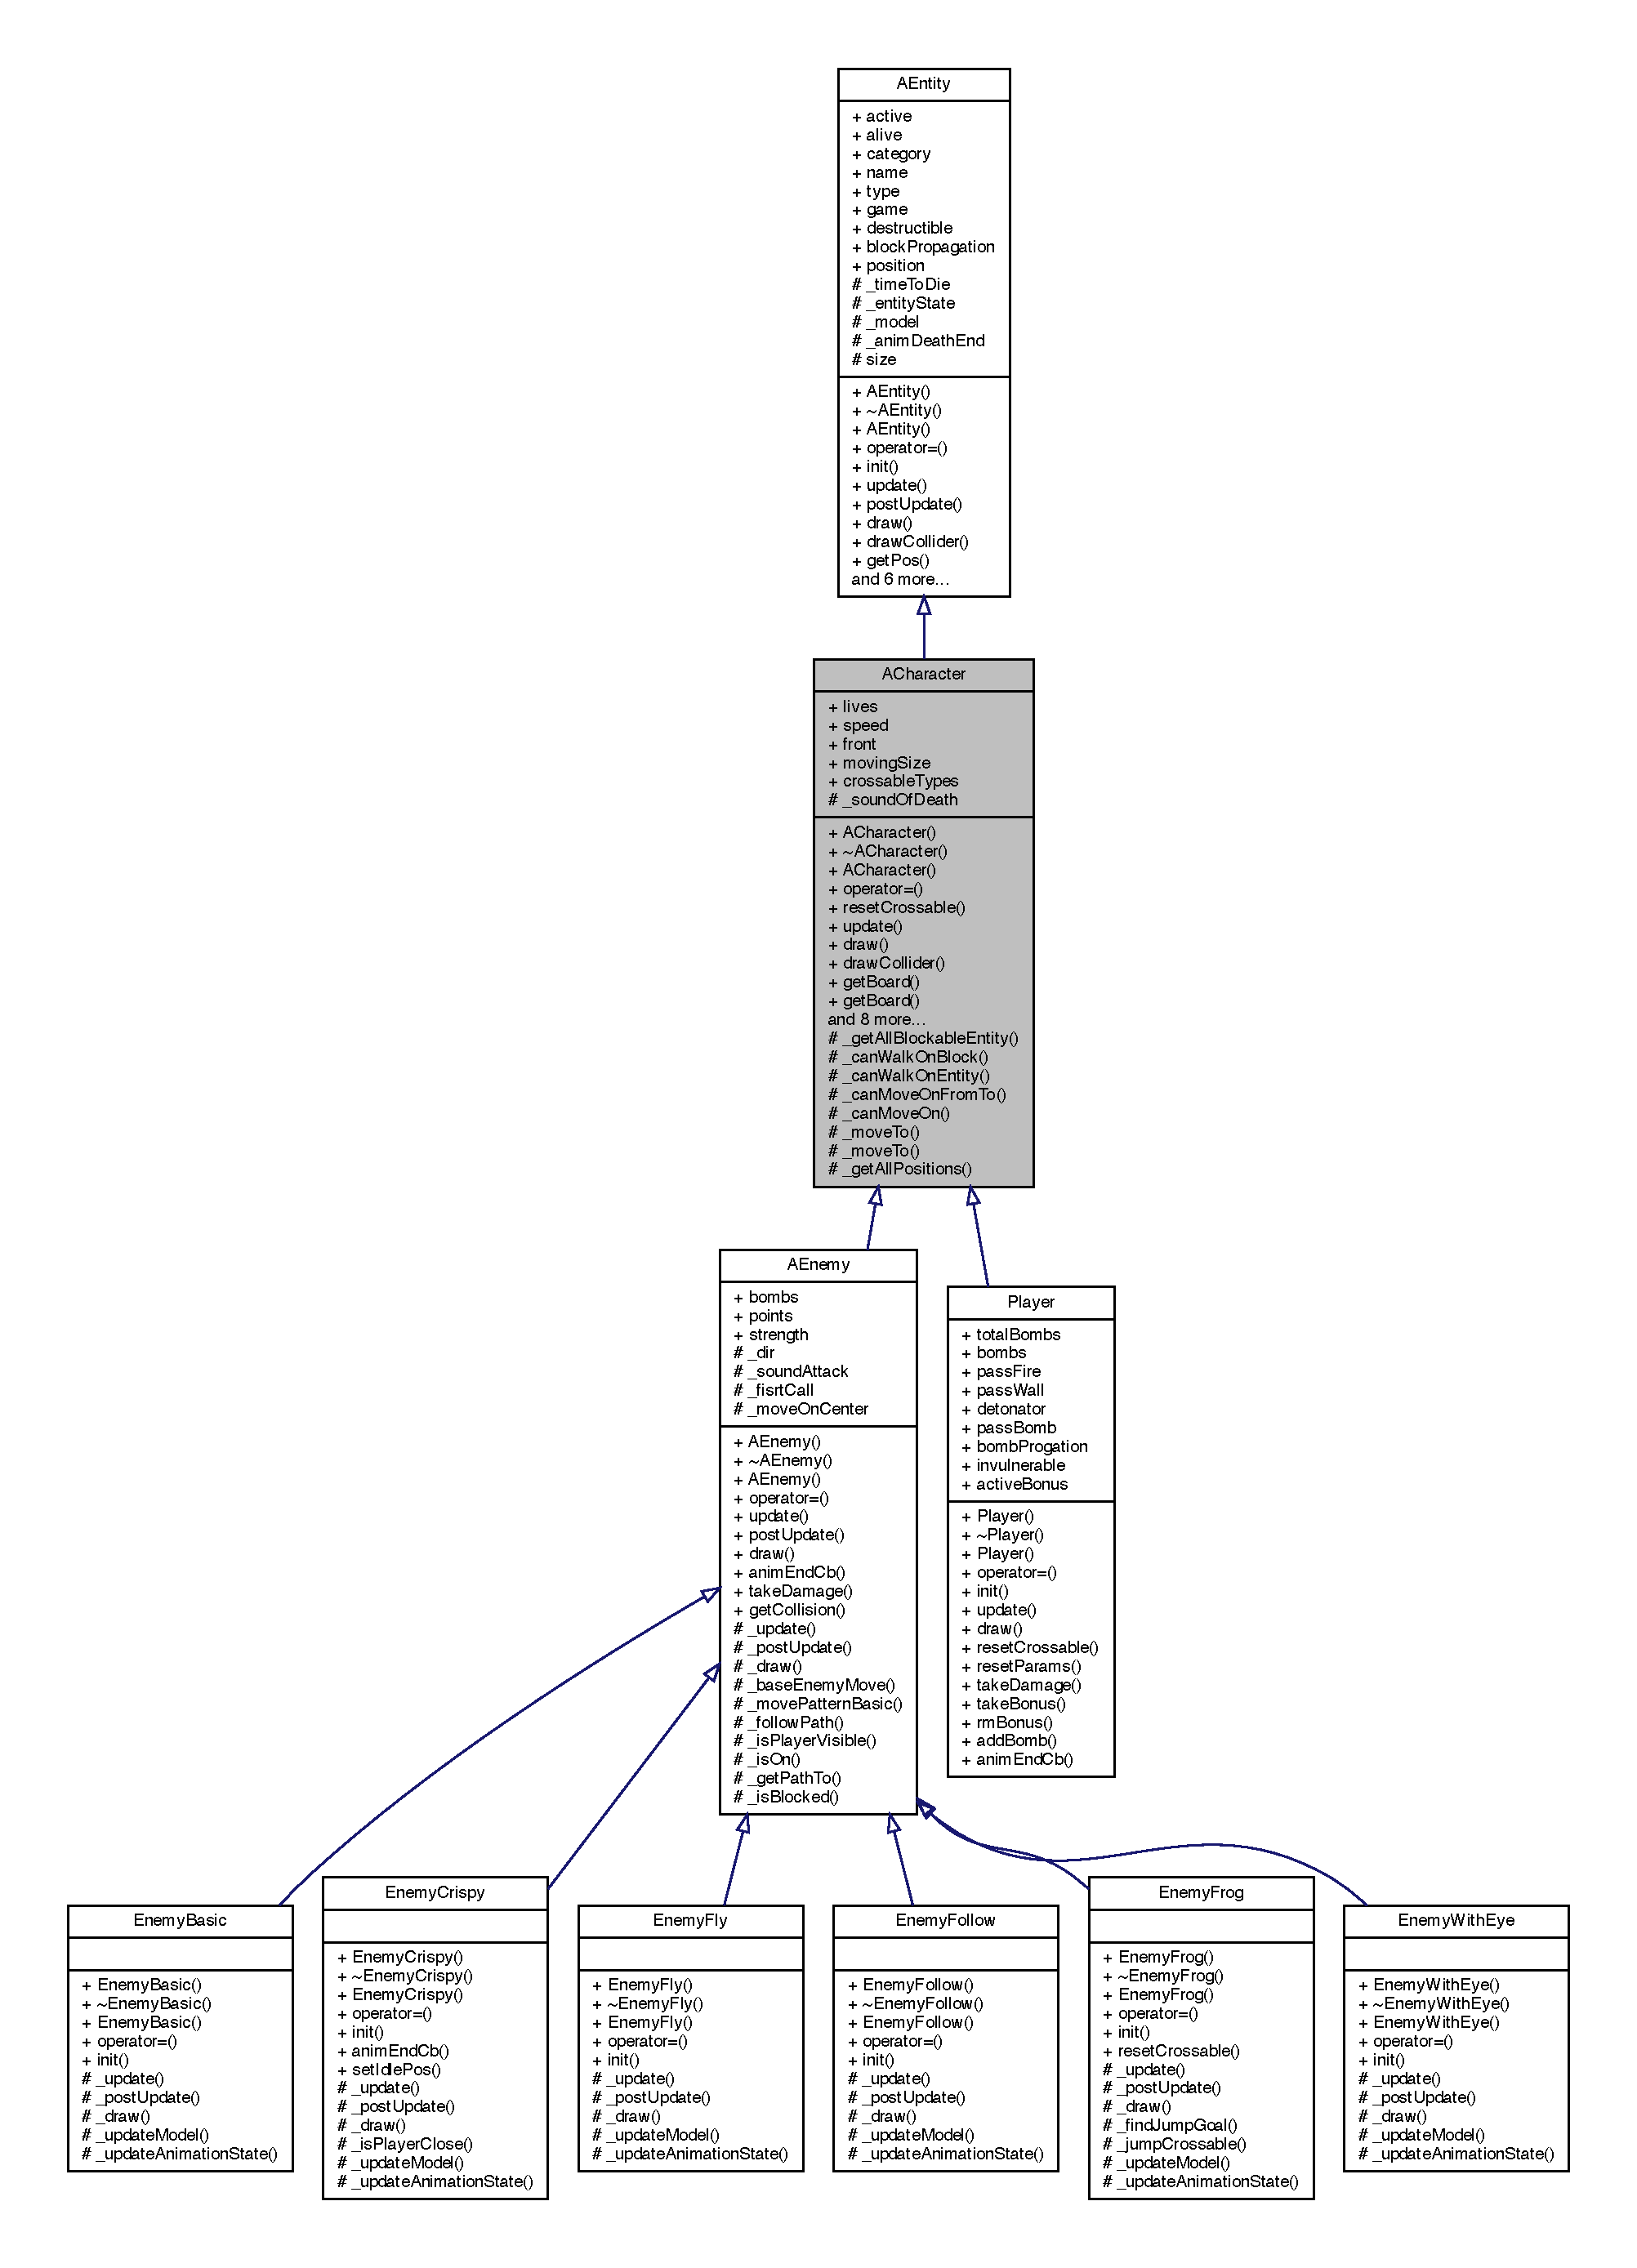
\includegraphics[width=350pt]{class_a_character__inherit__graph}
\end{center}
\end{figure}


Collaboration diagram for A\+Character\+:
\nopagebreak
\begin{figure}[H]
\begin{center}
\leavevmode
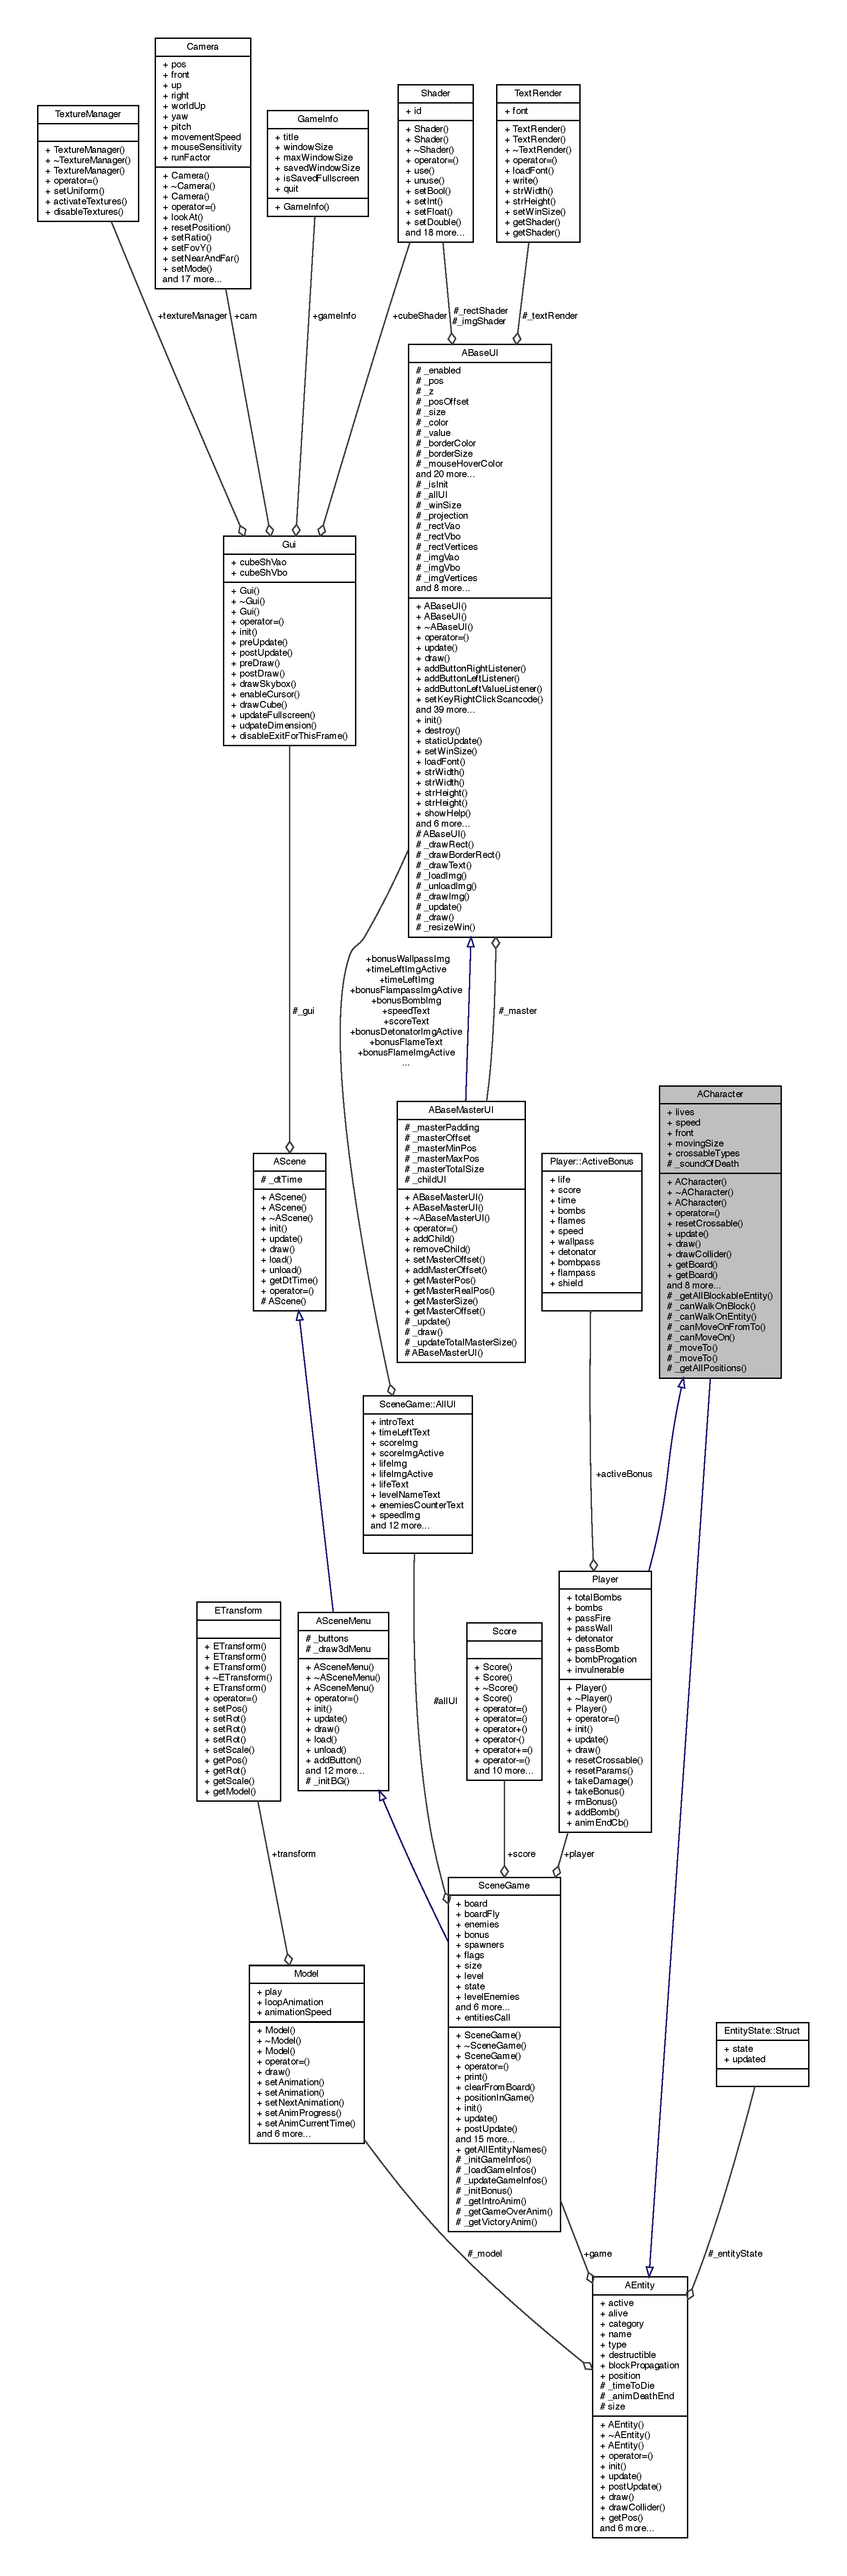
\includegraphics[height=550pt]{class_a_character__coll__graph}
\end{center}
\end{figure}
\doxysubsection*{Classes}
\begin{DoxyCompactItemize}
\item 
class \mbox{\hyperlink{class_a_character_1_1_a_character_exception}{A\+Character\+Exception}}
\end{DoxyCompactItemize}
\doxysubsection*{Public Member Functions}
\begin{DoxyCompactItemize}
\item 
\mbox{\Hypertarget{class_a_character_a110d0c6cd4cb1803d749e8638218790a}\label{class_a_character_a110d0c6cd4cb1803d749e8638218790a}} 
{\bfseries A\+Character} (\mbox{\hyperlink{class_scene_game}{Scene\+Game}} \&\mbox{\hyperlink{class_a_entity_aa2c05db944a8b7487eb8470dd20211ab}{game}})
\item 
\mbox{\Hypertarget{class_a_character_a157dffb2b05045b84dd3302267696bcd}\label{class_a_character_a157dffb2b05045b84dd3302267696bcd}} 
{\bfseries A\+Character} (\mbox{\hyperlink{class_a_character}{A\+Character}} const \&src)
\item 
\mbox{\Hypertarget{class_a_character_ad38be256f14ea4844adbcf4643837994}\label{class_a_character_ad38be256f14ea4844adbcf4643837994}} 
\mbox{\hyperlink{class_a_character}{A\+Character}} \& {\bfseries operator=} (\mbox{\hyperlink{class_a_character}{A\+Character}} const \&rhs)
\item 
\mbox{\Hypertarget{class_a_character_a8c942af7e72f1f0ac5e990e88da3ed4b}\label{class_a_character_a8c942af7e72f1f0ac5e990e88da3ed4b}} 
virtual void \mbox{\hyperlink{class_a_character_a8c942af7e72f1f0ac5e990e88da3ed4b}{reset\+Crossable}} ()
\begin{DoxyCompactList}\small\item\em Set the Entity that the Character can cross. \end{DoxyCompactList}\item 
\mbox{\Hypertarget{class_a_character_af5a4d00f6104d45b821a2e88b80936b5}\label{class_a_character_af5a4d00f6104d45b821a2e88b80936b5}} 
virtual bool {\bfseries update} ()=0
\item 
\mbox{\Hypertarget{class_a_character_af223d3c9dbd3143daf62e9834bd30e3d}\label{class_a_character_af223d3c9dbd3143daf62e9834bd30e3d}} 
virtual bool {\bfseries draw} (\mbox{\hyperlink{class_gui}{Gui}} \&gui)=0
\item 
virtual bool \mbox{\hyperlink{class_a_character_a2cc5faf1d9047d9e51154d5663fa6c67}{draw\+Collider}} ()
\begin{DoxyCompactList}\small\item\em Draw the collider of the entity. \end{DoxyCompactList}\item 
virtual std\+::vector$<$ std\+::vector$<$ std\+::vector$<$ \mbox{\hyperlink{class_a_entity}{A\+Entity}} $\ast$ $>$ $>$ $>$ const  \& \mbox{\hyperlink{class_a_character_adecb8064d5070f15a2d6aa76a151ff33}{get\+Board}} () const
\begin{DoxyCompactList}\small\item\em Get the board (game.\+board or game.\+board\+Fly) \end{DoxyCompactList}\item 
virtual std\+::vector$<$ std\+::vector$<$ std\+::vector$<$ \mbox{\hyperlink{class_a_entity}{A\+Entity}} $\ast$ $>$ $>$ $>$ \& \mbox{\hyperlink{class_a_character_aa8f0b9b557c69eead696870c41c8321b}{get\+Board}} ()
\begin{DoxyCompactList}\small\item\em Get the board (game.\+board or game.\+board\+Fly) \end{DoxyCompactList}\item 
bool \mbox{\hyperlink{class_a_character_a9a1508b5026652e36ebc72972317d576}{is\+Alive}} ()
\begin{DoxyCompactList}\small\item\em If the character still have lives, he is alive. \end{DoxyCompactList}\item 
glm\+::vec3 \mbox{\hyperlink{class_a_character_a41875fc55beaafd65fbe53ea3abc7f98}{get\+Pos}} () const
\begin{DoxyCompactList}\small\item\em Get the current postion of the \mbox{\hyperlink{class_a_character}{A\+Character}}. \end{DoxyCompactList}\item 
glm\+::ivec2 \mbox{\hyperlink{class_a_character_aa7562af195e3615c1f90488799687d9c}{get\+Int\+Pos}} () const
\begin{DoxyCompactList}\small\item\em Get the current position (in integer) \end{DoxyCompactList}\item 
\mbox{\hyperlink{class_a_character}{A\+Character}} $\ast$ \mbox{\hyperlink{class_a_character_a7e110857fc1e545a907d1e083431044a}{set\+Position}} (glm\+::vec3 pos)
\begin{DoxyCompactList}\small\item\em Init the Class. Needed to be called before any usage of the Class. \end{DoxyCompactList}\item 
virtual bool \mbox{\hyperlink{class_a_character_a1ab94580e4db621f79f0bf1d6bcdb600}{take\+Damage}} (const int damage)
\begin{DoxyCompactList}\small\item\em Character Take $<$damage$>$ damages. \end{DoxyCompactList}\item 
virtual std\+::unordered\+\_\+set$<$ \mbox{\hyperlink{class_a_entity}{A\+Entity}} $\ast$ $>$ \mbox{\hyperlink{class_a_character_a39c7111c4b096129d040e22e3b09592d}{get\+Collision}} (glm\+::vec3 dest) const
\begin{DoxyCompactList}\small\item\em get a list of entity in collision with the Character at a position. \end{DoxyCompactList}\item 
bool \mbox{\hyperlink{class_a_character_abf19d9677b90cd53bd3191b37939137d}{has\+Collision}} (glm\+::vec3 at\+Position, glm\+::vec3 at\+Size=glm\+::vec3(1, 1, 1))
\begin{DoxyCompactList}\small\item\em Test if Character have a collision at position $<$at\+Position$>$. \end{DoxyCompactList}\item 
bool \mbox{\hyperlink{class_a_character_a295783a792eedc09bcd68bc98eacb6d5}{tp}} (glm\+::vec3 tp\+Pos)
\begin{DoxyCompactList}\small\item\em Teleport a character on a position (tp check colision) \end{DoxyCompactList}\end{DoxyCompactItemize}
\doxysubsection*{Public Attributes}
\begin{DoxyCompactItemize}
\item 
\mbox{\Hypertarget{class_a_character_a46261a6f692a2b826ca0f30ccbdf93da}\label{class_a_character_a46261a6f692a2b826ca0f30ccbdf93da}} 
int {\bfseries lives}
\item 
\mbox{\Hypertarget{class_a_character_a078f65a8d5565962c2f17f44f19eef66}\label{class_a_character_a078f65a8d5565962c2f17f44f19eef66}} 
float {\bfseries speed}
\item 
\mbox{\Hypertarget{class_a_character_af8466a49b0a5abcc22a785562aed7257}\label{class_a_character_af8466a49b0a5abcc22a785562aed7257}} 
glm\+::vec3 {\bfseries front}
\item 
\mbox{\Hypertarget{class_a_character_ab91ce66f359d4c3fb605948689f4fd20}\label{class_a_character_ab91ce66f359d4c3fb605948689f4fd20}} 
glm\+::vec3 {\bfseries moving\+Size}
\item 
\mbox{\Hypertarget{class_a_character_a0a3b42d22279b8c13c6e9eab4f74da7b}\label{class_a_character_a0a3b42d22279b8c13c6e9eab4f74da7b}} 
std\+::vector$<$ Type\+::\+Enum $>$ {\bfseries crossable\+Types}
\end{DoxyCompactItemize}
\doxysubsection*{Protected Member Functions}
\begin{DoxyCompactItemize}
\item 
std\+::unordered\+\_\+set$<$ \mbox{\hyperlink{class_a_entity}{A\+Entity}} $\ast$ $>$ \mbox{\hyperlink{class_a_character_aef50edb318dc54c0fcccf053df180099}{\+\_\+get\+All\+Blockable\+Entity}} (glm\+::vec3 dest) const
\begin{DoxyCompactList}\small\item\em Get all entities that block the player on a given position. \end{DoxyCompactList}\item 
bool \mbox{\hyperlink{class_a_character_a82a72081a1261d749da88f4464757008}{\+\_\+can\+Walk\+On\+Block}} (glm\+::ivec2 pos) const
\begin{DoxyCompactList}\small\item\em Check if we can walk on a block. \end{DoxyCompactList}\item 
bool \mbox{\hyperlink{class_a_character_afce84f8aaaedb3f889f0d52e5f592ea8}{\+\_\+can\+Walk\+On\+Entity}} (\mbox{\hyperlink{class_a_entity}{A\+Entity}} $\ast$entity) const
\begin{DoxyCompactList}\small\item\em Check if we can walk on an entity. \end{DoxyCompactList}\item 
bool \mbox{\hyperlink{class_a_character_a771fdf0a7773de142d51ed599f3d557d}{\+\_\+can\+Move\+On\+From\+To}} (glm\+::vec3 from, glm\+::vec3 to) const
\begin{DoxyCompactList}\small\item\em Check if the entity can move on from a position to a destination. \end{DoxyCompactList}\item 
bool \mbox{\hyperlink{class_a_character_afbdeafa3e136320d980db3cf7f1fe7c7}{\+\_\+can\+Move\+On}} (glm\+::vec3 dest) const
\begin{DoxyCompactList}\small\item\em Check if the entity can move on a position. \end{DoxyCompactList}\item 
virtual glm\+::vec3 \mbox{\hyperlink{class_a_character_a4785e1688ede03fe488bfdfd3d2339ee}{\+\_\+move\+To}} (Direction\+::\+Enum direction, float const offset=O\+F\+F\+S\+E\+T\+\_\+\+T\+U\+R\+N\+\_\+\+C\+O\+R\+R\+E\+C\+T\+I\+ON)
\begin{DoxyCompactList}\small\item\em Move to direction if possible. \end{DoxyCompactList}\item 
virtual glm\+::vec3 \mbox{\hyperlink{class_a_character_a1a85eefb6e443e0e8a49ffb8e683659d}{\+\_\+move\+To}} (glm\+::vec3 direction, float const offset=O\+F\+F\+S\+E\+T\+\_\+\+T\+U\+R\+N\+\_\+\+C\+O\+R\+R\+E\+C\+T\+I\+ON)
\begin{DoxyCompactList}\small\item\em Move to direction if possible. \end{DoxyCompactList}\item 
std\+::vector$<$ glm\+::ivec2 $>$ \mbox{\hyperlink{class_a_character_ac90c6aeec198c760cba165860a67f622}{\+\_\+get\+All\+Positions}} (glm\+::vec3 dest, glm\+::vec3 \mbox{\hyperlink{class_a_entity_a47f976f25e6214669d64fb2bbb2c455a}{size}}) const
\begin{DoxyCompactList}\small\item\em get all positions blocks under character on a position \end{DoxyCompactList}\end{DoxyCompactItemize}
\doxysubsection*{Protected Attributes}
\begin{DoxyCompactItemize}
\item 
\mbox{\Hypertarget{class_a_character_a5af6eac92ea7539809748b6f9e4be83b}\label{class_a_character_a5af6eac92ea7539809748b6f9e4be83b}} 
std\+::string {\bfseries \+\_\+sound\+Of\+Death}
\end{DoxyCompactItemize}


\doxysubsection{Detailed Description}
This is the base for Charactere (\mbox{\hyperlink{class_player}{Player}}, AI, ...) 

\doxysubsection{Member Function Documentation}
\mbox{\Hypertarget{class_a_character_afbdeafa3e136320d980db3cf7f1fe7c7}\label{class_a_character_afbdeafa3e136320d980db3cf7f1fe7c7}} 
\index{ACharacter@{ACharacter}!\_canMoveOn@{\_canMoveOn}}
\index{\_canMoveOn@{\_canMoveOn}!ACharacter@{ACharacter}}
\doxysubsubsection{\texorpdfstring{\_canMoveOn()}{\_canMoveOn()}}
{\footnotesize\ttfamily bool A\+Character\+::\+\_\+can\+Move\+On (\begin{DoxyParamCaption}\item[{glm\+::vec3}]{dest }\end{DoxyParamCaption}) const\hspace{0.3cm}{\ttfamily [protected]}}



Check if the entity can move on a position. 


\begin{DoxyParams}{Parameters}
{\em dest} & The position to check \\
\hline
\end{DoxyParams}
\begin{DoxyReturn}{Returns}
true If the entity can move 
\end{DoxyReturn}
\mbox{\Hypertarget{class_a_character_a771fdf0a7773de142d51ed599f3d557d}\label{class_a_character_a771fdf0a7773de142d51ed599f3d557d}} 
\index{ACharacter@{ACharacter}!\_canMoveOnFromTo@{\_canMoveOnFromTo}}
\index{\_canMoveOnFromTo@{\_canMoveOnFromTo}!ACharacter@{ACharacter}}
\doxysubsubsection{\texorpdfstring{\_canMoveOnFromTo()}{\_canMoveOnFromTo()}}
{\footnotesize\ttfamily bool A\+Character\+::\+\_\+can\+Move\+On\+From\+To (\begin{DoxyParamCaption}\item[{glm\+::vec3}]{from,  }\item[{glm\+::vec3}]{to }\end{DoxyParamCaption}) const\hspace{0.3cm}{\ttfamily [protected]}}



Check if the entity can move on from a position to a destination. 

This function allow you to put bomb and walk on it


\begin{DoxyParams}{Parameters}
{\em from} & The actual position \\
\hline
{\em to} & The goal position \\
\hline
\end{DoxyParams}
\begin{DoxyReturn}{Returns}
true If the entity can move 
\end{DoxyReturn}
\mbox{\Hypertarget{class_a_character_a82a72081a1261d749da88f4464757008}\label{class_a_character_a82a72081a1261d749da88f4464757008}} 
\index{ACharacter@{ACharacter}!\_canWalkOnBlock@{\_canWalkOnBlock}}
\index{\_canWalkOnBlock@{\_canWalkOnBlock}!ACharacter@{ACharacter}}
\doxysubsubsection{\texorpdfstring{\_canWalkOnBlock()}{\_canWalkOnBlock()}}
{\footnotesize\ttfamily bool A\+Character\+::\+\_\+can\+Walk\+On\+Block (\begin{DoxyParamCaption}\item[{glm\+::ivec2}]{pos }\end{DoxyParamCaption}) const\hspace{0.3cm}{\ttfamily [protected]}}



Check if we can walk on a block. 


\begin{DoxyParams}{Parameters}
{\em pos} & The block pos \\
\hline
\end{DoxyParams}
\begin{DoxyReturn}{Returns}
true If we can walk on this block 
\end{DoxyReturn}
\mbox{\Hypertarget{class_a_character_afce84f8aaaedb3f889f0d52e5f592ea8}\label{class_a_character_afce84f8aaaedb3f889f0d52e5f592ea8}} 
\index{ACharacter@{ACharacter}!\_canWalkOnEntity@{\_canWalkOnEntity}}
\index{\_canWalkOnEntity@{\_canWalkOnEntity}!ACharacter@{ACharacter}}
\doxysubsubsection{\texorpdfstring{\_canWalkOnEntity()}{\_canWalkOnEntity()}}
{\footnotesize\ttfamily bool A\+Character\+::\+\_\+can\+Walk\+On\+Entity (\begin{DoxyParamCaption}\item[{\mbox{\hyperlink{class_a_entity}{A\+Entity}} $\ast$}]{entity }\end{DoxyParamCaption}) const\hspace{0.3cm}{\ttfamily [protected]}}



Check if we can walk on an entity. 


\begin{DoxyParams}{Parameters}
{\em pos} & The block pos \\
\hline
\end{DoxyParams}
\begin{DoxyReturn}{Returns}
true If we can walk on this block 
\end{DoxyReturn}
\mbox{\Hypertarget{class_a_character_aef50edb318dc54c0fcccf053df180099}\label{class_a_character_aef50edb318dc54c0fcccf053df180099}} 
\index{ACharacter@{ACharacter}!\_getAllBlockableEntity@{\_getAllBlockableEntity}}
\index{\_getAllBlockableEntity@{\_getAllBlockableEntity}!ACharacter@{ACharacter}}
\doxysubsubsection{\texorpdfstring{\_getAllBlockableEntity()}{\_getAllBlockableEntity()}}
{\footnotesize\ttfamily std\+::unordered\+\_\+set$<$ \mbox{\hyperlink{class_a_entity}{A\+Entity}} $\ast$ $>$ A\+Character\+::\+\_\+get\+All\+Blockable\+Entity (\begin{DoxyParamCaption}\item[{glm\+::vec3}]{dest }\end{DoxyParamCaption}) const\hspace{0.3cm}{\ttfamily [protected]}}



Get all entities that block the player on a given position. 

\begin{DoxyReturn}{Returns}
std\+::unordered\+\_\+set$<$\+A\+Entity $\ast$$>$ The list of entity 
\end{DoxyReturn}
\mbox{\Hypertarget{class_a_character_ac90c6aeec198c760cba165860a67f622}\label{class_a_character_ac90c6aeec198c760cba165860a67f622}} 
\index{ACharacter@{ACharacter}!\_getAllPositions@{\_getAllPositions}}
\index{\_getAllPositions@{\_getAllPositions}!ACharacter@{ACharacter}}
\doxysubsubsection{\texorpdfstring{\_getAllPositions()}{\_getAllPositions()}}
{\footnotesize\ttfamily std\+::vector$<$ glm\+::ivec2 $>$ A\+Character\+::\+\_\+get\+All\+Positions (\begin{DoxyParamCaption}\item[{glm\+::vec3}]{pos,  }\item[{glm\+::vec3}]{sz }\end{DoxyParamCaption}) const\hspace{0.3cm}{\ttfamily [protected]}}



get all positions blocks under character on a position 


\begin{DoxyParams}{Parameters}
{\em pos} & \\
\hline
{\em sz} & \\
\hline
\end{DoxyParams}
\begin{DoxyReturn}{Returns}
std\+::vector$<$glm\+::ivec2$>$ 
\end{DoxyReturn}
\mbox{\Hypertarget{class_a_character_a4785e1688ede03fe488bfdfd3d2339ee}\label{class_a_character_a4785e1688ede03fe488bfdfd3d2339ee}} 
\index{ACharacter@{ACharacter}!\_moveTo@{\_moveTo}}
\index{\_moveTo@{\_moveTo}!ACharacter@{ACharacter}}
\doxysubsubsection{\texorpdfstring{\_moveTo()}{\_moveTo()}\hspace{0.1cm}{\footnotesize\ttfamily [1/2]}}
{\footnotesize\ttfamily glm\+::vec3 A\+Character\+::\+\_\+move\+To (\begin{DoxyParamCaption}\item[{Direction\+::\+Enum}]{direction,  }\item[{float const}]{offset = {\ttfamily OFFSET\+\_\+TURN\+\_\+CORRECTION} }\end{DoxyParamCaption})\hspace{0.3cm}{\ttfamily [protected]}, {\ttfamily [virtual]}}



Move to direction if possible. 


\begin{DoxyParams}{Parameters}
{\em direction} & Direction to move \\
\hline
{\em offset} & Offset to turn correction (-\/1 to don\textquotesingle{}t use correction) \\
\hline
\end{DoxyParams}
\begin{DoxyReturn}{Returns}
glm\+::vec3 finale position 
\end{DoxyReturn}
\mbox{\Hypertarget{class_a_character_a1a85eefb6e443e0e8a49ffb8e683659d}\label{class_a_character_a1a85eefb6e443e0e8a49ffb8e683659d}} 
\index{ACharacter@{ACharacter}!\_moveTo@{\_moveTo}}
\index{\_moveTo@{\_moveTo}!ACharacter@{ACharacter}}
\doxysubsubsection{\texorpdfstring{\_moveTo()}{\_moveTo()}\hspace{0.1cm}{\footnotesize\ttfamily [2/2]}}
{\footnotesize\ttfamily glm\+::vec3 A\+Character\+::\+\_\+move\+To (\begin{DoxyParamCaption}\item[{glm\+::vec3}]{direction,  }\item[{float const}]{offset = {\ttfamily OFFSET\+\_\+TURN\+\_\+CORRECTION} }\end{DoxyParamCaption})\hspace{0.3cm}{\ttfamily [protected]}, {\ttfamily [virtual]}}



Move to direction if possible. 


\begin{DoxyParams}{Parameters}
{\em direction} & Direction to move \\
\hline
{\em offset} & Offset to turn correction (-\/1 to don\textquotesingle{}t use correction) \\
\hline
\end{DoxyParams}
\begin{DoxyReturn}{Returns}
glm\+::vec3 finale position 
\end{DoxyReturn}
\mbox{\Hypertarget{class_a_character_a2cc5faf1d9047d9e51154d5663fa6c67}\label{class_a_character_a2cc5faf1d9047d9e51154d5663fa6c67}} 
\index{ACharacter@{ACharacter}!drawCollider@{drawCollider}}
\index{drawCollider@{drawCollider}!ACharacter@{ACharacter}}
\doxysubsubsection{\texorpdfstring{drawCollider()}{drawCollider()}}
{\footnotesize\ttfamily bool A\+Character\+::draw\+Collider (\begin{DoxyParamCaption}{ }\end{DoxyParamCaption})\hspace{0.3cm}{\ttfamily [virtual]}}



Draw the collider of the entity. 

\begin{DoxyReturn}{Returns}
false If failed 
\end{DoxyReturn}


Reimplemented from \mbox{\hyperlink{class_a_entity_aca789d9c82a5fd3da3b196a36e748e8b}{A\+Entity}}.

\mbox{\Hypertarget{class_a_character_aa8f0b9b557c69eead696870c41c8321b}\label{class_a_character_aa8f0b9b557c69eead696870c41c8321b}} 
\index{ACharacter@{ACharacter}!getBoard@{getBoard}}
\index{getBoard@{getBoard}!ACharacter@{ACharacter}}
\doxysubsubsection{\texorpdfstring{getBoard()}{getBoard()}\hspace{0.1cm}{\footnotesize\ttfamily [1/2]}}
{\footnotesize\ttfamily std\+::vector$<$ std\+::vector$<$ std\+::vector$<$ \mbox{\hyperlink{class_a_entity}{A\+Entity}} $\ast$ $>$ $>$ $>$ \& A\+Character\+::get\+Board (\begin{DoxyParamCaption}{ }\end{DoxyParamCaption})\hspace{0.3cm}{\ttfamily [virtual]}}



Get the board (game.\+board or game.\+board\+Fly) 

\begin{DoxyReturn}{Returns}
std\+::vector$<$ std\+::vector$<$ std\+::vector$<$\+A\+Entity $\ast$$>$ $>$ $>$\& A reference to the board 
\end{DoxyReturn}


Implements \mbox{\hyperlink{class_a_entity}{A\+Entity}}.

\mbox{\Hypertarget{class_a_character_adecb8064d5070f15a2d6aa76a151ff33}\label{class_a_character_adecb8064d5070f15a2d6aa76a151ff33}} 
\index{ACharacter@{ACharacter}!getBoard@{getBoard}}
\index{getBoard@{getBoard}!ACharacter@{ACharacter}}
\doxysubsubsection{\texorpdfstring{getBoard()}{getBoard()}\hspace{0.1cm}{\footnotesize\ttfamily [2/2]}}
{\footnotesize\ttfamily std\+::vector$<$ std\+::vector$<$ std\+::vector$<$ \mbox{\hyperlink{class_a_entity}{A\+Entity}} $\ast$ $>$ $>$ $>$ const  \& A\+Character\+::get\+Board (\begin{DoxyParamCaption}{ }\end{DoxyParamCaption}) const\hspace{0.3cm}{\ttfamily [virtual]}}



Get the board (game.\+board or game.\+board\+Fly) 

\begin{DoxyReturn}{Returns}
std\+::vector$<$ std\+::vector$<$ std\+::vector$<$\+A\+Entity $\ast$$>$ $>$ $>$\& A reference to the board 
\end{DoxyReturn}


Implements \mbox{\hyperlink{class_a_entity}{A\+Entity}}.

\mbox{\Hypertarget{class_a_character_a39c7111c4b096129d040e22e3b09592d}\label{class_a_character_a39c7111c4b096129d040e22e3b09592d}} 
\index{ACharacter@{ACharacter}!getCollision@{getCollision}}
\index{getCollision@{getCollision}!ACharacter@{ACharacter}}
\doxysubsubsection{\texorpdfstring{getCollision()}{getCollision()}}
{\footnotesize\ttfamily std\+::unordered\+\_\+set$<$ \mbox{\hyperlink{class_a_entity}{A\+Entity}} $\ast$ $>$ A\+Character\+::get\+Collision (\begin{DoxyParamCaption}\item[{glm\+::vec3}]{dest }\end{DoxyParamCaption}) const\hspace{0.3cm}{\ttfamily [virtual]}}



get a list of entity in collision with the Character at a position. 


\begin{DoxyParams}{Parameters}
{\em pos} & default V\+O\+I\+D\+\_\+\+P\+O\+S3 \\
\hline
\end{DoxyParams}
\begin{DoxyReturn}{Returns}
std\+::unordered\+\_\+set$<$\+A\+Entity $\ast$$>$ collisions 
\end{DoxyReturn}


Reimplemented in \mbox{\hyperlink{class_a_enemy_aca840427bf701f3c24b38a4c17a14cfd}{A\+Enemy}}.

\mbox{\Hypertarget{class_a_character_aa7562af195e3615c1f90488799687d9c}\label{class_a_character_aa7562af195e3615c1f90488799687d9c}} 
\index{ACharacter@{ACharacter}!getIntPos@{getIntPos}}
\index{getIntPos@{getIntPos}!ACharacter@{ACharacter}}
\doxysubsubsection{\texorpdfstring{getIntPos()}{getIntPos()}}
{\footnotesize\ttfamily glm\+::ivec2 A\+Character\+::get\+Int\+Pos (\begin{DoxyParamCaption}{ }\end{DoxyParamCaption}) const}



Get the current position (in integer) 

\begin{DoxyReturn}{Returns}
glm\+::ivec2 The integer position 
\end{DoxyReturn}
\mbox{\Hypertarget{class_a_character_a41875fc55beaafd65fbe53ea3abc7f98}\label{class_a_character_a41875fc55beaafd65fbe53ea3abc7f98}} 
\index{ACharacter@{ACharacter}!getPos@{getPos}}
\index{getPos@{getPos}!ACharacter@{ACharacter}}
\doxysubsubsection{\texorpdfstring{getPos()}{getPos()}}
{\footnotesize\ttfamily glm\+::vec3 A\+Character\+::get\+Pos (\begin{DoxyParamCaption}{ }\end{DoxyParamCaption}) const\hspace{0.3cm}{\ttfamily [virtual]}}



Get the current postion of the \mbox{\hyperlink{class_a_character}{A\+Character}}. 

\begin{DoxyReturn}{Returns}
glm\+::vec2 
\end{DoxyReturn}


Implements \mbox{\hyperlink{class_a_entity}{A\+Entity}}.

\mbox{\Hypertarget{class_a_character_abf19d9677b90cd53bd3191b37939137d}\label{class_a_character_abf19d9677b90cd53bd3191b37939137d}} 
\index{ACharacter@{ACharacter}!hasCollision@{hasCollision}}
\index{hasCollision@{hasCollision}!ACharacter@{ACharacter}}
\doxysubsubsection{\texorpdfstring{hasCollision()}{hasCollision()}}
{\footnotesize\ttfamily bool A\+Character\+::has\+Collision (\begin{DoxyParamCaption}\item[{glm\+::vec3}]{at\+Position,  }\item[{glm\+::vec3}]{at\+Size = {\ttfamily glm\+:\+:vec3(1,~1,~1)} }\end{DoxyParamCaption})}



Test if Character have a collision at position $<$at\+Position$>$. 


\begin{DoxyParams}{Parameters}
{\em at\+Position} & \\
\hline
{\em at\+Size} & \\
\hline
\end{DoxyParams}
\begin{DoxyReturn}{Returns}
true if has a collision 

false if no collision 
\end{DoxyReturn}
\mbox{\Hypertarget{class_a_character_a9a1508b5026652e36ebc72972317d576}\label{class_a_character_a9a1508b5026652e36ebc72972317d576}} 
\index{ACharacter@{ACharacter}!isAlive@{isAlive}}
\index{isAlive@{isAlive}!ACharacter@{ACharacter}}
\doxysubsubsection{\texorpdfstring{isAlive()}{isAlive()}}
{\footnotesize\ttfamily bool A\+Character\+::is\+Alive (\begin{DoxyParamCaption}{ }\end{DoxyParamCaption})}



If the character still have lives, he is alive. 

\begin{DoxyReturn}{Returns}
true if alive 

false if dead 
\end{DoxyReturn}
\mbox{\Hypertarget{class_a_character_a7e110857fc1e545a907d1e083431044a}\label{class_a_character_a7e110857fc1e545a907d1e083431044a}} 
\index{ACharacter@{ACharacter}!setPosition@{setPosition}}
\index{setPosition@{setPosition}!ACharacter@{ACharacter}}
\doxysubsubsection{\texorpdfstring{setPosition()}{setPosition()}}
{\footnotesize\ttfamily \mbox{\hyperlink{class_a_character}{A\+Character}} $\ast$ A\+Character\+::set\+Position (\begin{DoxyParamCaption}\item[{glm\+::vec3}]{pos }\end{DoxyParamCaption})}



Init the Class. Needed to be called before any usage of the Class. 


\begin{DoxyParams}{Parameters}
{\em pos} & \\
\hline
\end{DoxyParams}
\begin{DoxyReturn}{Returns}
A\+Character$\ast$ 
\end{DoxyReturn}
\mbox{\Hypertarget{class_a_character_a1ab94580e4db621f79f0bf1d6bcdb600}\label{class_a_character_a1ab94580e4db621f79f0bf1d6bcdb600}} 
\index{ACharacter@{ACharacter}!takeDamage@{takeDamage}}
\index{takeDamage@{takeDamage}!ACharacter@{ACharacter}}
\doxysubsubsection{\texorpdfstring{takeDamage()}{takeDamage()}}
{\footnotesize\ttfamily bool A\+Character\+::take\+Damage (\begin{DoxyParamCaption}\item[{const int}]{damage }\end{DoxyParamCaption})\hspace{0.3cm}{\ttfamily [virtual]}}



Character Take $<$damage$>$ damages. 


\begin{DoxyParams}{Parameters}
{\em damage} & \\
\hline
\end{DoxyParams}
\begin{DoxyReturn}{Returns}
true if damage taken 

false if damage not taken 
\end{DoxyReturn}


Implements \mbox{\hyperlink{class_a_entity}{A\+Entity}}.



Reimplemented in \mbox{\hyperlink{class_a_enemy_a17bcf116c42c3d780e243127adf1a947}{A\+Enemy}}, and \mbox{\hyperlink{class_player_a029b1d511340697d8ccfb7bfa604435b}{Player}}.

\mbox{\Hypertarget{class_a_character_a295783a792eedc09bcd68bc98eacb6d5}\label{class_a_character_a295783a792eedc09bcd68bc98eacb6d5}} 
\index{ACharacter@{ACharacter}!tp@{tp}}
\index{tp@{tp}!ACharacter@{ACharacter}}
\doxysubsubsection{\texorpdfstring{tp()}{tp()}}
{\footnotesize\ttfamily bool A\+Character\+::tp (\begin{DoxyParamCaption}\item[{glm\+::vec3}]{tp\+Pos }\end{DoxyParamCaption})}



Teleport a character on a position (tp check colision) 


\begin{DoxyParams}{Parameters}
{\em tp\+Pos} & The position to teleport \\
\hline
\end{DoxyParams}
\begin{DoxyReturn}{Returns}
true If the tp is a success 
\end{DoxyReturn}


The documentation for this class was generated from the following files\+:\begin{DoxyCompactItemize}
\item 
includes/A\+Character.\+hpp\item 
srcs/A\+Character.\+cpp\end{DoxyCompactItemize}

\hypertarget{class_a_character_1_1_a_character_exception}{}\doxysection{A\+Character\+::A\+Character\+Exception Class Reference}
\label{class_a_character_1_1_a_character_exception}\index{ACharacter::ACharacterException@{ACharacter::ACharacterException}}
Inheritance diagram for A\+Character\+::A\+Character\+Exception\+:\begin{figure}[H]
\begin{center}
\leavevmode
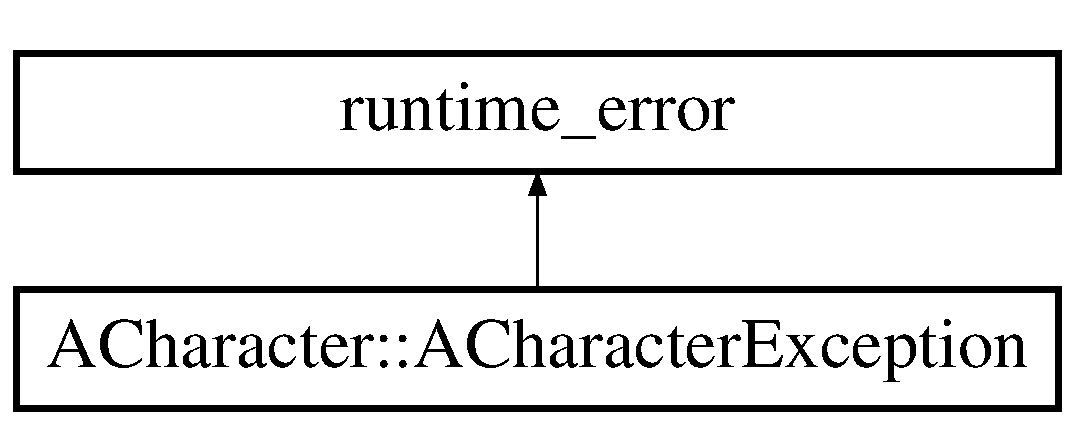
\includegraphics[height=2.000000cm]{class_a_character_1_1_a_character_exception}
\end{center}
\end{figure}
\doxysubsection*{Public Member Functions}
\begin{DoxyCompactItemize}
\item 
\mbox{\Hypertarget{class_a_character_1_1_a_character_exception_ae56dd5eaef5224676e077e51af7099bd}\label{class_a_character_1_1_a_character_exception_ae56dd5eaef5224676e077e51af7099bd}} 
{\bfseries A\+Character\+Exception} (const char $\ast$what\+\_\+arg)
\end{DoxyCompactItemize}


The documentation for this class was generated from the following files\+:\begin{DoxyCompactItemize}
\item 
includes/A\+Character.\+hpp\item 
srcs/A\+Character.\+cpp\end{DoxyCompactItemize}

\hypertarget{struct_player_1_1_active_bonus}{}\doxysection{Player\+::Active\+Bonus Struct Reference}
\label{struct_player_1_1_active_bonus}\index{Player::ActiveBonus@{Player::ActiveBonus}}


All active bonus for the player.  




{\ttfamily \#include $<$Player.\+hpp$>$}



Collaboration diagram for Player\+::Active\+Bonus\+:
\nopagebreak
\begin{figure}[H]
\begin{center}
\leavevmode
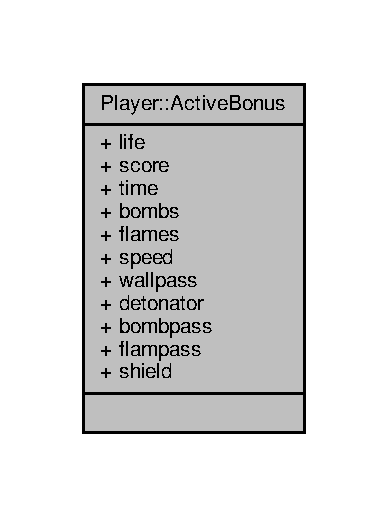
\includegraphics[width=186pt]{struct_player_1_1_active_bonus__coll__graph}
\end{center}
\end{figure}
\doxysubsection*{Public Attributes}
\begin{DoxyCompactItemize}
\item 
float \mbox{\hyperlink{struct_player_1_1_active_bonus_a692c7135db9ad842843290ee5dcbac89}{life}}
\item 
float \mbox{\hyperlink{struct_player_1_1_active_bonus_adfe7670def68cc0126c258b7a3f86d05}{score}}
\item 
float \mbox{\hyperlink{struct_player_1_1_active_bonus_a4d5933b2c052d233a8ee9934577f6fdd}{time}}
\item 
float \mbox{\hyperlink{struct_player_1_1_active_bonus_a64e48a895e5b25afe0ac4ae485ce4d72}{bombs}}
\item 
float \mbox{\hyperlink{struct_player_1_1_active_bonus_a1211f1a048e0c7ae2c19db42c8ddf66b}{flames}}
\item 
float \mbox{\hyperlink{struct_player_1_1_active_bonus_a317b13d54c4fb53345a60fb2f4f747ce}{speed}}
\item 
float \mbox{\hyperlink{struct_player_1_1_active_bonus_af5a24d36905852ddac53dfea2712e81d}{wallpass}}
\item 
float \mbox{\hyperlink{struct_player_1_1_active_bonus_a6aa16b9216e018365e36bedbc77c759b}{detonator}}
\item 
float \mbox{\hyperlink{struct_player_1_1_active_bonus_ad82ff4f3afc445717eaf75a07c899fb3}{bombpass}}
\item 
float \mbox{\hyperlink{struct_player_1_1_active_bonus_a5e2f4f07c50fc159c16270e9fc1d4d5c}{flampass}}
\item 
float \mbox{\hyperlink{struct_player_1_1_active_bonus_acb8273d2a958ca83d8799ce2bc3e9491}{shield}}
\end{DoxyCompactItemize}


\doxysubsection{Detailed Description}
All active bonus for the player. 

\doxysubsection{Member Data Documentation}
\mbox{\Hypertarget{struct_player_1_1_active_bonus_ad82ff4f3afc445717eaf75a07c899fb3}\label{struct_player_1_1_active_bonus_ad82ff4f3afc445717eaf75a07c899fb3}} 
\index{Player::ActiveBonus@{Player::ActiveBonus}!bombpass@{bombpass}}
\index{bombpass@{bombpass}!Player::ActiveBonus@{Player::ActiveBonus}}
\doxysubsubsection{\texorpdfstring{bombpass}{bombpass}}
{\footnotesize\ttfamily float Player\+::\+Active\+Bonus\+::bombpass}

\mbox{\hyperlink{class_player}{Player}} bombpass \mbox{\Hypertarget{struct_player_1_1_active_bonus_a64e48a895e5b25afe0ac4ae485ce4d72}\label{struct_player_1_1_active_bonus_a64e48a895e5b25afe0ac4ae485ce4d72}} 
\index{Player::ActiveBonus@{Player::ActiveBonus}!bombs@{bombs}}
\index{bombs@{bombs}!Player::ActiveBonus@{Player::ActiveBonus}}
\doxysubsubsection{\texorpdfstring{bombs}{bombs}}
{\footnotesize\ttfamily float Player\+::\+Active\+Bonus\+::bombs}

\mbox{\hyperlink{class_player}{Player}} bombs \mbox{\Hypertarget{struct_player_1_1_active_bonus_a6aa16b9216e018365e36bedbc77c759b}\label{struct_player_1_1_active_bonus_a6aa16b9216e018365e36bedbc77c759b}} 
\index{Player::ActiveBonus@{Player::ActiveBonus}!detonator@{detonator}}
\index{detonator@{detonator}!Player::ActiveBonus@{Player::ActiveBonus}}
\doxysubsubsection{\texorpdfstring{detonator}{detonator}}
{\footnotesize\ttfamily float Player\+::\+Active\+Bonus\+::detonator}

\mbox{\hyperlink{class_player}{Player}} detonator \mbox{\Hypertarget{struct_player_1_1_active_bonus_a1211f1a048e0c7ae2c19db42c8ddf66b}\label{struct_player_1_1_active_bonus_a1211f1a048e0c7ae2c19db42c8ddf66b}} 
\index{Player::ActiveBonus@{Player::ActiveBonus}!flames@{flames}}
\index{flames@{flames}!Player::ActiveBonus@{Player::ActiveBonus}}
\doxysubsubsection{\texorpdfstring{flames}{flames}}
{\footnotesize\ttfamily float Player\+::\+Active\+Bonus\+::flames}

\mbox{\hyperlink{class_player}{Player}} bomb propagation \mbox{\Hypertarget{struct_player_1_1_active_bonus_a5e2f4f07c50fc159c16270e9fc1d4d5c}\label{struct_player_1_1_active_bonus_a5e2f4f07c50fc159c16270e9fc1d4d5c}} 
\index{Player::ActiveBonus@{Player::ActiveBonus}!flampass@{flampass}}
\index{flampass@{flampass}!Player::ActiveBonus@{Player::ActiveBonus}}
\doxysubsubsection{\texorpdfstring{flampass}{flampass}}
{\footnotesize\ttfamily float Player\+::\+Active\+Bonus\+::flampass}

\mbox{\hyperlink{class_player}{Player}} flampass \mbox{\Hypertarget{struct_player_1_1_active_bonus_a692c7135db9ad842843290ee5dcbac89}\label{struct_player_1_1_active_bonus_a692c7135db9ad842843290ee5dcbac89}} 
\index{Player::ActiveBonus@{Player::ActiveBonus}!life@{life}}
\index{life@{life}!Player::ActiveBonus@{Player::ActiveBonus}}
\doxysubsubsection{\texorpdfstring{life}{life}}
{\footnotesize\ttfamily float Player\+::\+Active\+Bonus\+::life}

\mbox{\hyperlink{class_player}{Player}} life \mbox{\Hypertarget{struct_player_1_1_active_bonus_adfe7670def68cc0126c258b7a3f86d05}\label{struct_player_1_1_active_bonus_adfe7670def68cc0126c258b7a3f86d05}} 
\index{Player::ActiveBonus@{Player::ActiveBonus}!score@{score}}
\index{score@{score}!Player::ActiveBonus@{Player::ActiveBonus}}
\doxysubsubsection{\texorpdfstring{score}{score}}
{\footnotesize\ttfamily float Player\+::\+Active\+Bonus\+::score}

\mbox{\hyperlink{class_player}{Player}} score \mbox{\Hypertarget{struct_player_1_1_active_bonus_acb8273d2a958ca83d8799ce2bc3e9491}\label{struct_player_1_1_active_bonus_acb8273d2a958ca83d8799ce2bc3e9491}} 
\index{Player::ActiveBonus@{Player::ActiveBonus}!shield@{shield}}
\index{shield@{shield}!Player::ActiveBonus@{Player::ActiveBonus}}
\doxysubsubsection{\texorpdfstring{shield}{shield}}
{\footnotesize\ttfamily float Player\+::\+Active\+Bonus\+::shield}

\mbox{\hyperlink{class_player}{Player}} shield \mbox{\Hypertarget{struct_player_1_1_active_bonus_a317b13d54c4fb53345a60fb2f4f747ce}\label{struct_player_1_1_active_bonus_a317b13d54c4fb53345a60fb2f4f747ce}} 
\index{Player::ActiveBonus@{Player::ActiveBonus}!speed@{speed}}
\index{speed@{speed}!Player::ActiveBonus@{Player::ActiveBonus}}
\doxysubsubsection{\texorpdfstring{speed}{speed}}
{\footnotesize\ttfamily float Player\+::\+Active\+Bonus\+::speed}

\mbox{\hyperlink{class_player}{Player}} speed \mbox{\Hypertarget{struct_player_1_1_active_bonus_a4d5933b2c052d233a8ee9934577f6fdd}\label{struct_player_1_1_active_bonus_a4d5933b2c052d233a8ee9934577f6fdd}} 
\index{Player::ActiveBonus@{Player::ActiveBonus}!time@{time}}
\index{time@{time}!Player::ActiveBonus@{Player::ActiveBonus}}
\doxysubsubsection{\texorpdfstring{time}{time}}
{\footnotesize\ttfamily float Player\+::\+Active\+Bonus\+::time}

\mbox{\hyperlink{class_player}{Player}} time left to do level \mbox{\Hypertarget{struct_player_1_1_active_bonus_af5a24d36905852ddac53dfea2712e81d}\label{struct_player_1_1_active_bonus_af5a24d36905852ddac53dfea2712e81d}} 
\index{Player::ActiveBonus@{Player::ActiveBonus}!wallpass@{wallpass}}
\index{wallpass@{wallpass}!Player::ActiveBonus@{Player::ActiveBonus}}
\doxysubsubsection{\texorpdfstring{wallpass}{wallpass}}
{\footnotesize\ttfamily float Player\+::\+Active\+Bonus\+::wallpass}

\mbox{\hyperlink{class_player}{Player}} wallpass 

The documentation for this struct was generated from the following file\+:\begin{DoxyCompactItemize}
\item 
includes/elements/Player.\+hpp\end{DoxyCompactItemize}

\hypertarget{class_a_enemy}{}\doxysection{A\+Enemy Class Reference}
\label{class_a_enemy}\index{AEnemy@{AEnemy}}


This is the base enemy object.  




{\ttfamily \#include $<$A\+Enemy.\+hpp$>$}



Inheritance diagram for A\+Enemy\+:
\nopagebreak
\begin{figure}[H]
\begin{center}
\leavevmode
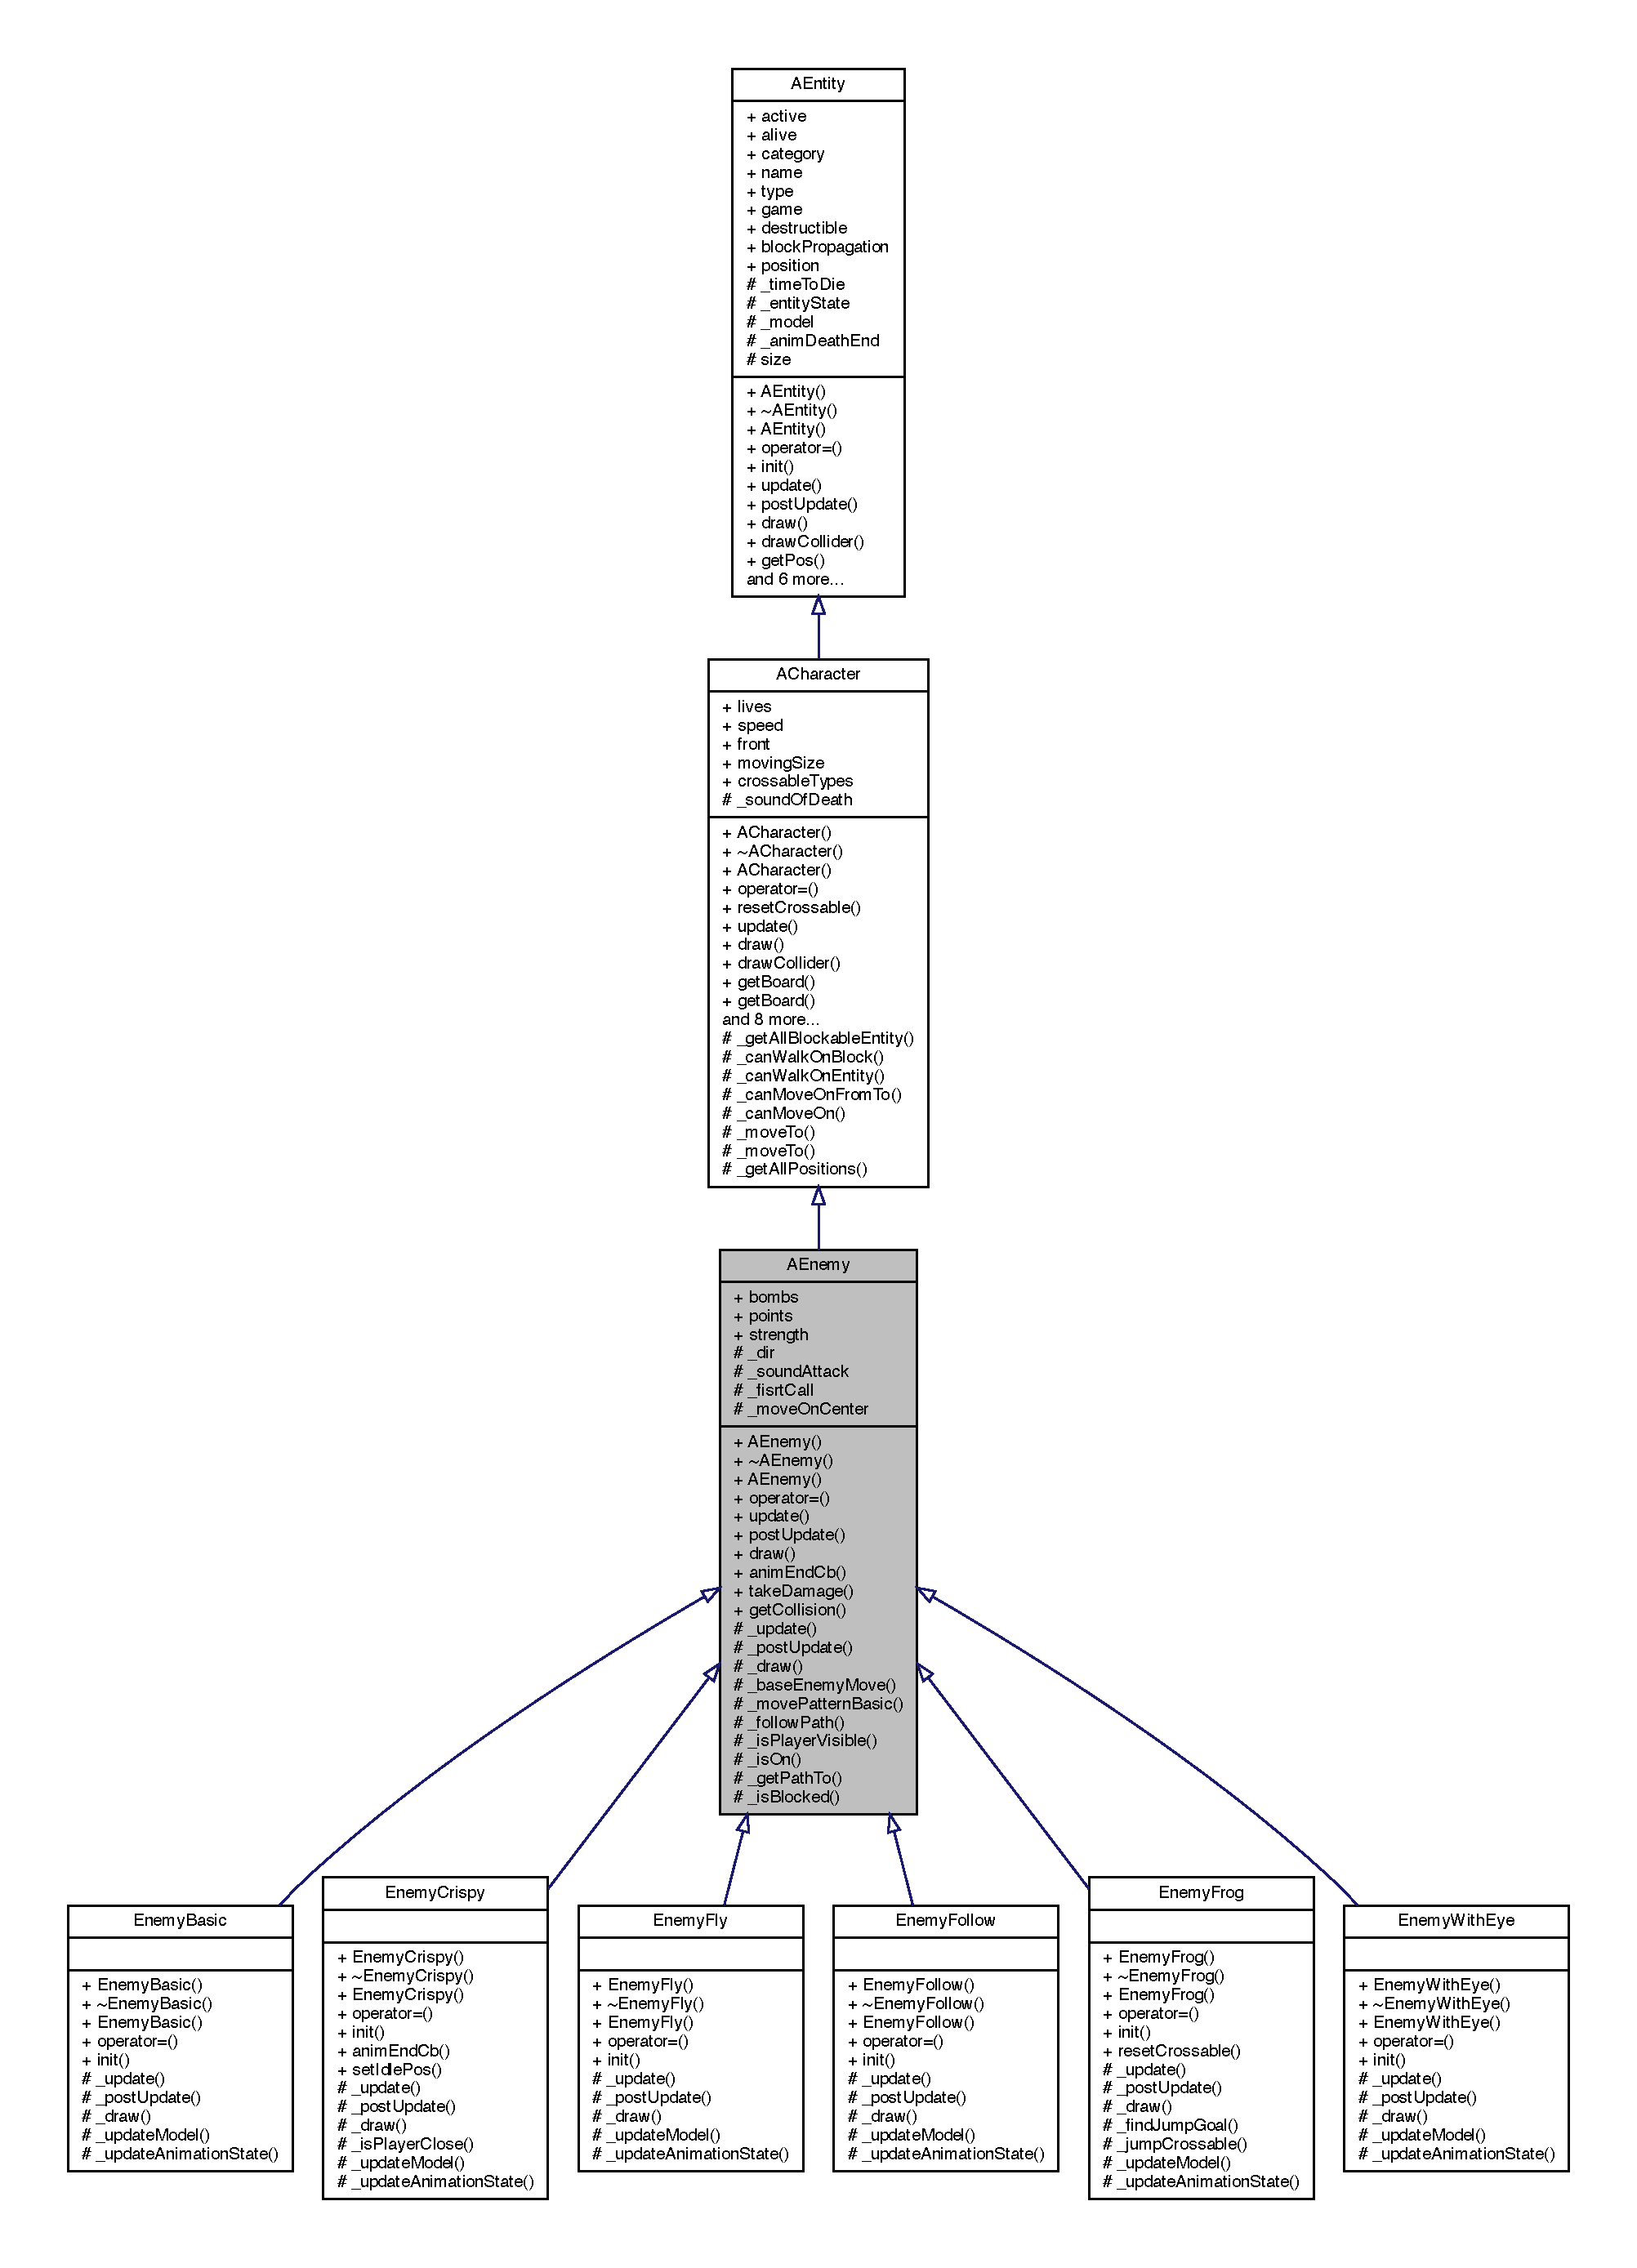
\includegraphics[width=350pt]{class_a_enemy__inherit__graph}
\end{center}
\end{figure}


Collaboration diagram for A\+Enemy\+:
\nopagebreak
\begin{figure}[H]
\begin{center}
\leavevmode
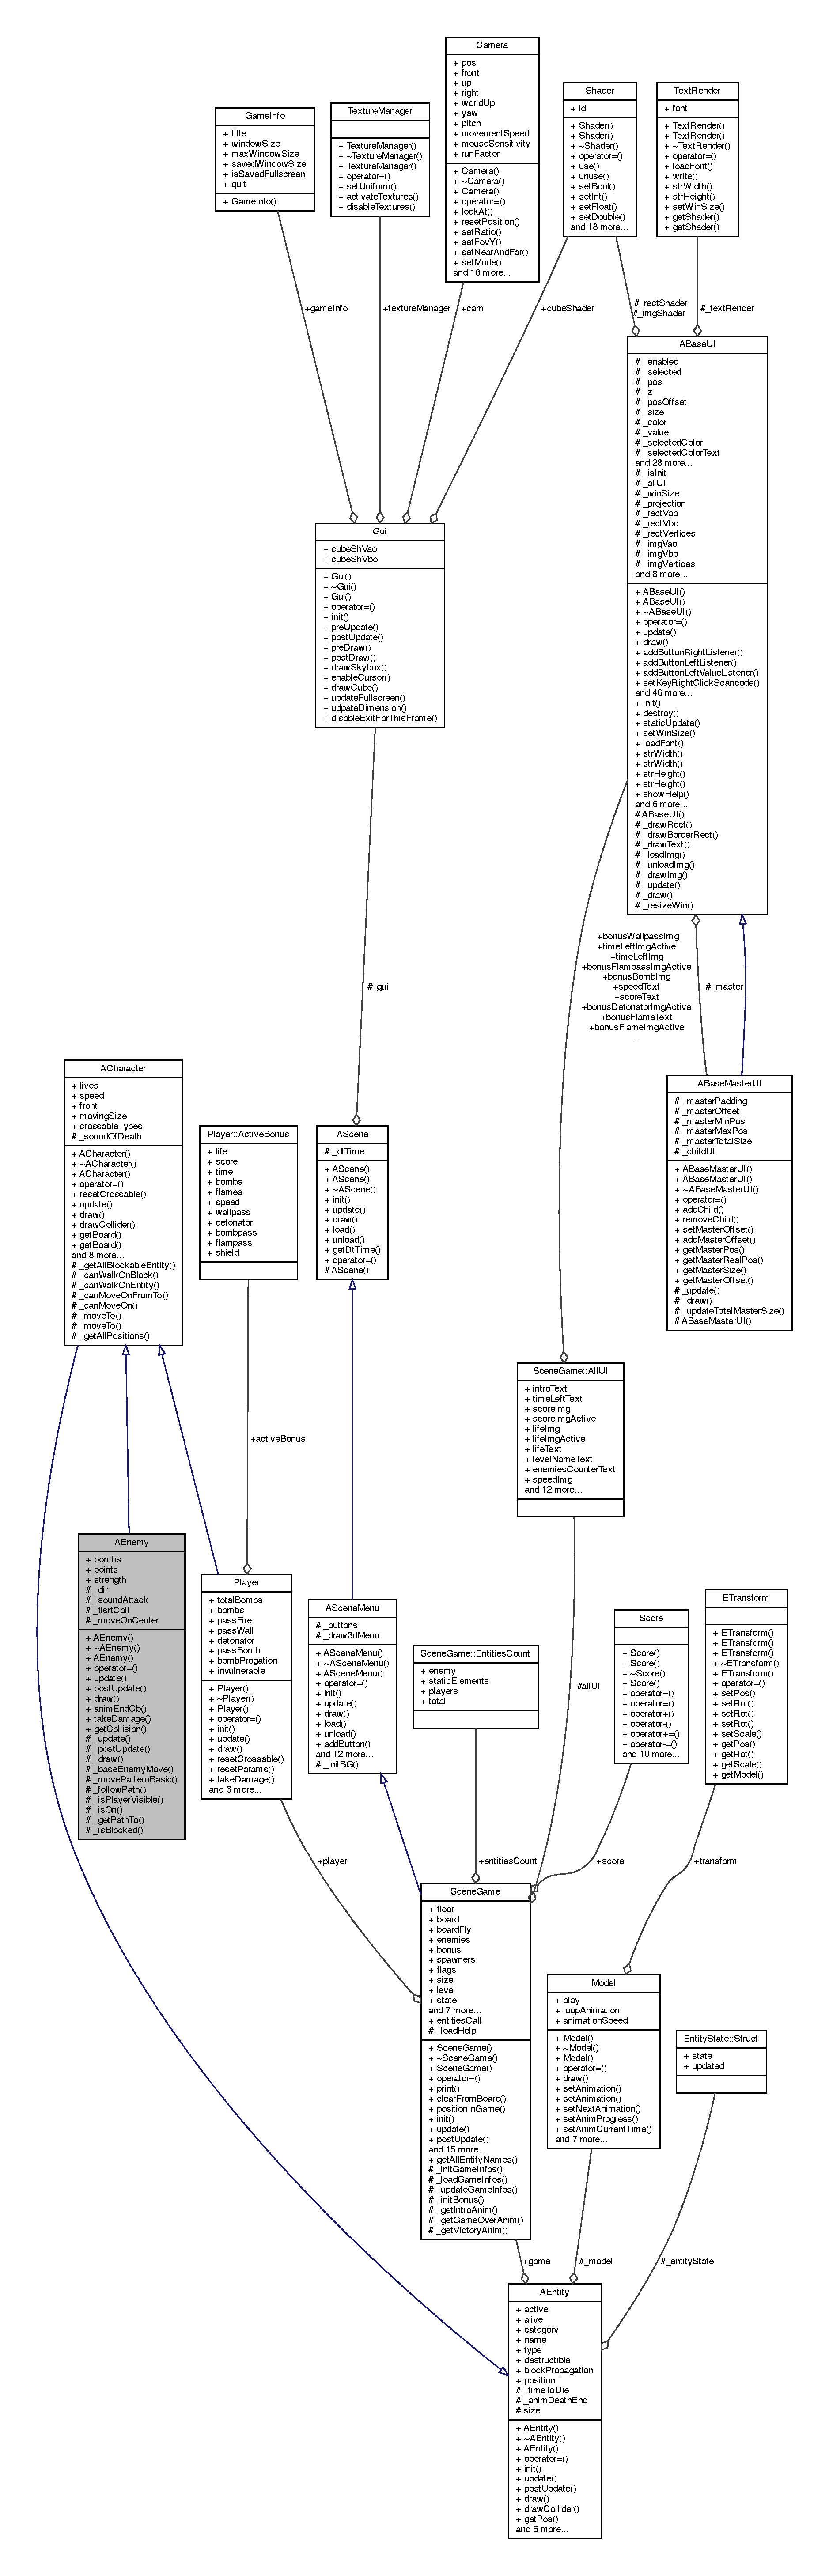
\includegraphics[height=550pt]{class_a_enemy__coll__graph}
\end{center}
\end{figure}
\doxysubsection*{Classes}
\begin{DoxyCompactItemize}
\item 
class \mbox{\hyperlink{class_a_enemy_1_1_enemy_exception}{Enemy\+Exception}}
\end{DoxyCompactItemize}
\doxysubsection*{Public Member Functions}
\begin{DoxyCompactItemize}
\item 
\mbox{\Hypertarget{class_a_enemy_a951b8e4a3fbd53542740f8ba3f01b79d}\label{class_a_enemy_a951b8e4a3fbd53542740f8ba3f01b79d}} 
{\bfseries A\+Enemy} (\mbox{\hyperlink{class_scene_game}{Scene\+Game}} \&\mbox{\hyperlink{class_a_entity_aa2c05db944a8b7487eb8470dd20211ab}{game}})
\item 
\mbox{\Hypertarget{class_a_enemy_add417acf741a28c3896fce4ffbad2e2a}\label{class_a_enemy_add417acf741a28c3896fce4ffbad2e2a}} 
{\bfseries A\+Enemy} (\mbox{\hyperlink{class_a_enemy}{A\+Enemy}} const \&src)
\item 
\mbox{\Hypertarget{class_a_enemy_a87e3db110aa11d461768f794bfb48c40}\label{class_a_enemy_a87e3db110aa11d461768f794bfb48c40}} 
\mbox{\hyperlink{class_a_enemy}{A\+Enemy}} \& {\bfseries operator=} (\mbox{\hyperlink{class_a_enemy}{A\+Enemy}} const \&rhs)
\item 
bool \mbox{\hyperlink{class_a_enemy_a01e3b0313d6f29bf2cafe20f711c0550}{update}} ()
\begin{DoxyCompactList}\small\item\em update is called each frame. \end{DoxyCompactList}\item 
bool \mbox{\hyperlink{class_a_enemy_a2d2ff5a126f14294bdbc17475c363d00}{post\+Update}} ()
\begin{DoxyCompactList}\small\item\em post\+Update is called each frame. After \mbox{\hyperlink{class_a_enemy_a01e3b0313d6f29bf2cafe20f711c0550}{update()}} \end{DoxyCompactList}\item 
bool \mbox{\hyperlink{class_a_enemy_a527fc4b7bb46c04c486fd025a01e16a9}{draw}} (\mbox{\hyperlink{class_gui}{Gui}} \&gui)
\begin{DoxyCompactList}\small\item\em draw is called each frame. \end{DoxyCompactList}\item 
virtual void \mbox{\hyperlink{class_a_enemy_ac946b6cd7d96f99365301450566d3baf}{anim\+End\+Cb}} (std\+::string anim\+Name)
\begin{DoxyCompactList}\small\item\em called on animation end if passed to \mbox{\hyperlink{class_model}{Model}} \end{DoxyCompactList}\item 
virtual bool \mbox{\hyperlink{class_a_enemy_a17bcf116c42c3d780e243127adf1a947}{take\+Damage}} (const int damage)
\begin{DoxyCompactList}\small\item\em \mbox{\hyperlink{class_a_enemy}{A\+Enemy}} Take $<$damage$>$ damages. \end{DoxyCompactList}\item 
std\+::unordered\+\_\+set$<$ \mbox{\hyperlink{class_a_entity}{A\+Entity}} $\ast$ $>$ \mbox{\hyperlink{class_a_enemy_aca840427bf701f3c24b38a4c17a14cfd}{get\+Collision}} (glm\+::vec3 dest) const
\begin{DoxyCompactList}\small\item\em get a list of entity in collision with the Character at a position. \end{DoxyCompactList}\end{DoxyCompactItemize}
\doxysubsection*{Public Attributes}
\begin{DoxyCompactItemize}
\item 
\mbox{\Hypertarget{class_a_enemy_ac306e77e93cd7574766e04d17728d18a}\label{class_a_enemy_ac306e77e93cd7574766e04d17728d18a}} 
int {\bfseries bombs}
\item 
\mbox{\Hypertarget{class_a_enemy_a0d6c03c5f76b67b821f2510cc12dfc64}\label{class_a_enemy_a0d6c03c5f76b67b821f2510cc12dfc64}} 
int32\+\_\+t {\bfseries points}
\item 
\mbox{\Hypertarget{class_a_enemy_ac1bb9d347e62e478c9c83be27dcf1598}\label{class_a_enemy_ac1bb9d347e62e478c9c83be27dcf1598}} 
int {\bfseries strength}
\end{DoxyCompactItemize}
\doxysubsection*{Protected Member Functions}
\begin{DoxyCompactItemize}
\item 
\mbox{\Hypertarget{class_a_enemy_abefc22131eb1c618819c67c3c1415c08}\label{class_a_enemy_abefc22131eb1c618819c67c3c1415c08}} 
virtual bool {\bfseries \+\_\+update} ()=0
\item 
\mbox{\Hypertarget{class_a_enemy_a78b010638f552c4ab11ff71e7b826b1b}\label{class_a_enemy_a78b010638f552c4ab11ff71e7b826b1b}} 
virtual bool {\bfseries \+\_\+post\+Update} ()=0
\item 
\mbox{\Hypertarget{class_a_enemy_a70e3638b5ed8ecea2a087ffe16510dd2}\label{class_a_enemy_a70e3638b5ed8ecea2a087ffe16510dd2}} 
virtual bool {\bfseries \+\_\+draw} (\mbox{\hyperlink{class_gui}{Gui}} \&gui)=0
\item 
bool \mbox{\hyperlink{class_a_enemy_aff49d7d4a833983ede184276ebf93b67}{\+\_\+base\+Enemy\+Move}} (Direction\+::\+Enum \&dir)
\begin{DoxyCompactList}\small\item\em Base moving function for enemy. \end{DoxyCompactList}\item 
bool \mbox{\hyperlink{class_a_enemy_a2ddbe01e55094dbbff085ff10b1db957}{\+\_\+move\+Pattern\+Basic}} (std\+::vector$<$ Direction\+::\+Enum $>$ direction\+Order, uint32\+\_\+t \&dir\+Idx)
\begin{DoxyCompactList}\small\item\em Move and follow a basic pattern (list of direction). \end{DoxyCompactList}\item 
bool \mbox{\hyperlink{class_a_enemy_ae9fafd83ac6040298120c6e3a8656743}{\+\_\+follow\+Path}} (std\+::deque$<$ \mbox{\hyperlink{struct_path_node}{Path\+Node}} $>$ \&path)
\begin{DoxyCompactList}\small\item\em Follow the given path. \end{DoxyCompactList}\item 
Direction\+::\+Enum \mbox{\hyperlink{class_a_enemy_a7909b6882d5dba58d147decadc256cba}{\+\_\+is\+Player\+Visible}} () const
\begin{DoxyCompactList}\small\item\em If the player is visible by the entity, return the direction of the player. \end{DoxyCompactList}\item 
bool \mbox{\hyperlink{class_a_enemy_a250a33c7294ac9d6b125eebe8acd51e3}{\+\_\+is\+On}} (glm\+::ivec2 dest, float offset=I\+S\+\_\+\+O\+N\+\_\+\+P\+O\+S\+\_\+\+O\+F\+F\+S\+ET) const
\begin{DoxyCompactList}\small\item\em Check if the enemy is on dest. \end{DoxyCompactList}\item 
bool \mbox{\hyperlink{class_a_enemy_a5ff3b836a7a98499a1a4019f7238b4d0}{\+\_\+get\+Path\+To}} (glm\+::ivec2 dest, std\+::deque$<$ \mbox{\hyperlink{struct_path_node}{Path\+Node}} $>$ \&path)
\begin{DoxyCompactList}\small\item\em Get the path to a destination. \end{DoxyCompactList}\item 
bool \mbox{\hyperlink{class_a_enemy_a4348865dc5c245e2d88e31296847e1a6}{\+\_\+is\+Blocked}} ()
\begin{DoxyCompactList}\small\item\em Check if the enemy is blocked btw walls. \end{DoxyCompactList}\end{DoxyCompactItemize}
\doxysubsection*{Protected Attributes}
\begin{DoxyCompactItemize}
\item 
\mbox{\Hypertarget{class_a_enemy_af85a958024c72d9c0f522be466c75092}\label{class_a_enemy_af85a958024c72d9c0f522be466c75092}} 
Direction\+::\+Enum {\bfseries \+\_\+dir}
\item 
\mbox{\Hypertarget{class_a_enemy_a4b3d010b8630c401730fbee2bfeb2a6b}\label{class_a_enemy_a4b3d010b8630c401730fbee2bfeb2a6b}} 
std\+::vector$<$ std\+::string $>$ {\bfseries \+\_\+sound\+Attack}
\item 
\mbox{\Hypertarget{class_a_enemy_a112cb8a927706e1a563119258239f4b6}\label{class_a_enemy_a112cb8a927706e1a563119258239f4b6}} 
bool {\bfseries \+\_\+fisrt\+Call}
\item 
\mbox{\Hypertarget{class_a_enemy_af05841272b0bfa864dcfffaeb1e29a9b}\label{class_a_enemy_af05841272b0bfa864dcfffaeb1e29a9b}} 
bool {\bfseries \+\_\+move\+On\+Center}
\end{DoxyCompactItemize}


\doxysubsection{Detailed Description}
This is the base enemy object. 

\doxysubsection{Member Function Documentation}
\mbox{\Hypertarget{class_a_enemy_aff49d7d4a833983ede184276ebf93b67}\label{class_a_enemy_aff49d7d4a833983ede184276ebf93b67}} 
\index{AEnemy@{AEnemy}!\_baseEnemyMove@{\_baseEnemyMove}}
\index{\_baseEnemyMove@{\_baseEnemyMove}!AEnemy@{AEnemy}}
\doxysubsubsection{\texorpdfstring{\_baseEnemyMove()}{\_baseEnemyMove()}}
{\footnotesize\ttfamily bool A\+Enemy\+::\+\_\+base\+Enemy\+Move (\begin{DoxyParamCaption}\item[{Direction\+::\+Enum \&}]{dir }\end{DoxyParamCaption})\hspace{0.3cm}{\ttfamily [protected]}}



Base moving function for enemy. 


\begin{DoxyParams}{Parameters}
{\em dir} & The actual direction of the enemy \\
\hline
\end{DoxyParams}
\begin{DoxyReturn}{Returns}
false If the enemy is blocked 
\end{DoxyReturn}
\mbox{\Hypertarget{class_a_enemy_ae9fafd83ac6040298120c6e3a8656743}\label{class_a_enemy_ae9fafd83ac6040298120c6e3a8656743}} 
\index{AEnemy@{AEnemy}!\_followPath@{\_followPath}}
\index{\_followPath@{\_followPath}!AEnemy@{AEnemy}}
\doxysubsubsection{\texorpdfstring{\_followPath()}{\_followPath()}}
{\footnotesize\ttfamily bool A\+Enemy\+::\+\_\+follow\+Path (\begin{DoxyParamCaption}\item[{std\+::deque$<$ \mbox{\hyperlink{struct_path_node}{Path\+Node}} $>$ \&}]{path }\end{DoxyParamCaption})\hspace{0.3cm}{\ttfamily [protected]}}



Follow the given path. 


\begin{DoxyParams}{Parameters}
{\em path} & The path to follow \\
\hline
\end{DoxyParams}
\begin{DoxyReturn}{Returns}
false If the Entity is blocked 
\end{DoxyReturn}
\mbox{\Hypertarget{class_a_enemy_a5ff3b836a7a98499a1a4019f7238b4d0}\label{class_a_enemy_a5ff3b836a7a98499a1a4019f7238b4d0}} 
\index{AEnemy@{AEnemy}!\_getPathTo@{\_getPathTo}}
\index{\_getPathTo@{\_getPathTo}!AEnemy@{AEnemy}}
\doxysubsubsection{\texorpdfstring{\_getPathTo()}{\_getPathTo()}}
{\footnotesize\ttfamily bool A\+Enemy\+::\+\_\+get\+Path\+To (\begin{DoxyParamCaption}\item[{glm\+::ivec2}]{dest,  }\item[{std\+::deque$<$ \mbox{\hyperlink{struct_path_node}{Path\+Node}} $>$ \&}]{path }\end{DoxyParamCaption})\hspace{0.3cm}{\ttfamily [protected]}}



Get the path to a destination. 


\begin{DoxyParams}{Parameters}
{\em dest} & The destination \\
\hline
{\em path} & The path (empty if there is no path). \\
\hline
\end{DoxyParams}
\begin{DoxyReturn}{Returns}
true if a path is detected 
\end{DoxyReturn}
\mbox{\Hypertarget{class_a_enemy_a4348865dc5c245e2d88e31296847e1a6}\label{class_a_enemy_a4348865dc5c245e2d88e31296847e1a6}} 
\index{AEnemy@{AEnemy}!\_isBlocked@{\_isBlocked}}
\index{\_isBlocked@{\_isBlocked}!AEnemy@{AEnemy}}
\doxysubsubsection{\texorpdfstring{\_isBlocked()}{\_isBlocked()}}
{\footnotesize\ttfamily bool A\+Enemy\+::\+\_\+is\+Blocked (\begin{DoxyParamCaption}{ }\end{DoxyParamCaption})\hspace{0.3cm}{\ttfamily [protected]}}



Check if the enemy is blocked btw walls. 

\begin{DoxyReturn}{Returns}
true If the enemy is blocked 
\end{DoxyReturn}
\mbox{\Hypertarget{class_a_enemy_a250a33c7294ac9d6b125eebe8acd51e3}\label{class_a_enemy_a250a33c7294ac9d6b125eebe8acd51e3}} 
\index{AEnemy@{AEnemy}!\_isOn@{\_isOn}}
\index{\_isOn@{\_isOn}!AEnemy@{AEnemy}}
\doxysubsubsection{\texorpdfstring{\_isOn()}{\_isOn()}}
{\footnotesize\ttfamily bool A\+Enemy\+::\+\_\+is\+On (\begin{DoxyParamCaption}\item[{glm\+::ivec2}]{dest,  }\item[{float}]{offset = {\ttfamily IS\+\_\+ON\+\_\+POS\+\_\+OFFSET} }\end{DoxyParamCaption}) const\hspace{0.3cm}{\ttfamily [protected]}}



Check if the enemy is on dest. 


\begin{DoxyParams}{Parameters}
{\em dest} & The postion to compare with enemy pos \\
\hline
\end{DoxyParams}
\begin{DoxyReturn}{Returns}
true If is on the destination 
\end{DoxyReturn}
\mbox{\Hypertarget{class_a_enemy_a7909b6882d5dba58d147decadc256cba}\label{class_a_enemy_a7909b6882d5dba58d147decadc256cba}} 
\index{AEnemy@{AEnemy}!\_isPlayerVisible@{\_isPlayerVisible}}
\index{\_isPlayerVisible@{\_isPlayerVisible}!AEnemy@{AEnemy}}
\doxysubsubsection{\texorpdfstring{\_isPlayerVisible()}{\_isPlayerVisible()}}
{\footnotesize\ttfamily Direction\+::\+Enum A\+Enemy\+::\+\_\+is\+Player\+Visible (\begin{DoxyParamCaption}{ }\end{DoxyParamCaption}) const\hspace{0.3cm}{\ttfamily [protected]}}



If the player is visible by the entity, return the direction of the player. 

\begin{DoxyReturn}{Returns}
Direction\+::\+Enum Return the direction of the player (N\+O\+\_\+\+D\+I\+R\+E\+C\+T\+I\+ON if not visible) 
\end{DoxyReturn}
\mbox{\Hypertarget{class_a_enemy_a2ddbe01e55094dbbff085ff10b1db957}\label{class_a_enemy_a2ddbe01e55094dbbff085ff10b1db957}} 
\index{AEnemy@{AEnemy}!\_movePatternBasic@{\_movePatternBasic}}
\index{\_movePatternBasic@{\_movePatternBasic}!AEnemy@{AEnemy}}
\doxysubsubsection{\texorpdfstring{\_movePatternBasic()}{\_movePatternBasic()}}
{\footnotesize\ttfamily bool A\+Enemy\+::\+\_\+move\+Pattern\+Basic (\begin{DoxyParamCaption}\item[{std\+::vector$<$ Direction\+::\+Enum $>$}]{direction\+Order,  }\item[{uint32\+\_\+t \&}]{dir\+Idx }\end{DoxyParamCaption})\hspace{0.3cm}{\ttfamily [protected]}}



Move and follow a basic pattern (list of direction). 

start at direction\+Order\mbox{[}start\+Dir\+ID\mbox{]} and try to move. If cannot move, try all the next direction until one direction is valid.


\begin{DoxyParams}{Parameters}
{\em direction\+Order} & A vector with all direction in the right order \\
\hline
{\em dir\+Idx} & The direction used (index in direction\+Order) \\
\hline
\end{DoxyParams}
\begin{DoxyReturn}{Returns}
false If the enemy is blocked 
\end{DoxyReturn}
\mbox{\Hypertarget{class_a_enemy_ac946b6cd7d96f99365301450566d3baf}\label{class_a_enemy_ac946b6cd7d96f99365301450566d3baf}} 
\index{AEnemy@{AEnemy}!animEndCb@{animEndCb}}
\index{animEndCb@{animEndCb}!AEnemy@{AEnemy}}
\doxysubsubsection{\texorpdfstring{animEndCb()}{animEndCb()}}
{\footnotesize\ttfamily void A\+Enemy\+::anim\+End\+Cb (\begin{DoxyParamCaption}\item[{std\+::string}]{anim\+Name }\end{DoxyParamCaption})\hspace{0.3cm}{\ttfamily [virtual]}}



called on animation end if passed to \mbox{\hyperlink{class_model}{Model}} 


\begin{DoxyParams}{Parameters}
{\em anim\+Name} & the current animation name \\
\hline
\end{DoxyParams}


Reimplemented from \mbox{\hyperlink{class_a_entity_ac1fd0bdb4c01a4767660f03cd06cd2ac}{A\+Entity}}.



Reimplemented in \mbox{\hyperlink{class_enemy_crispy_a32d938b70f4b0f2bd2e1df606c812d13}{Enemy\+Crispy}}.

\mbox{\Hypertarget{class_a_enemy_a527fc4b7bb46c04c486fd025a01e16a9}\label{class_a_enemy_a527fc4b7bb46c04c486fd025a01e16a9}} 
\index{AEnemy@{AEnemy}!draw@{draw}}
\index{draw@{draw}!AEnemy@{AEnemy}}
\doxysubsubsection{\texorpdfstring{draw()}{draw()}}
{\footnotesize\ttfamily bool A\+Enemy\+::draw (\begin{DoxyParamCaption}\item[{\mbox{\hyperlink{class_gui}{Gui}} \&}]{gui }\end{DoxyParamCaption})\hspace{0.3cm}{\ttfamily [virtual]}}



draw is called each frame. 

\begin{DoxyReturn}{Returns}
true if success 

false if failure 
\end{DoxyReturn}


Implements \mbox{\hyperlink{class_a_character}{A\+Character}}.

\mbox{\Hypertarget{class_a_enemy_aca840427bf701f3c24b38a4c17a14cfd}\label{class_a_enemy_aca840427bf701f3c24b38a4c17a14cfd}} 
\index{AEnemy@{AEnemy}!getCollision@{getCollision}}
\index{getCollision@{getCollision}!AEnemy@{AEnemy}}
\doxysubsubsection{\texorpdfstring{getCollision()}{getCollision()}}
{\footnotesize\ttfamily std\+::unordered\+\_\+set$<$ \mbox{\hyperlink{class_a_entity}{A\+Entity}} $\ast$ $>$ A\+Enemy\+::get\+Collision (\begin{DoxyParamCaption}\item[{glm\+::vec3}]{dest }\end{DoxyParamCaption}) const\hspace{0.3cm}{\ttfamily [virtual]}}



get a list of entity in collision with the Character at a position. 


\begin{DoxyParams}{Parameters}
{\em pos} & default V\+O\+I\+D\+\_\+\+P\+O\+S3 \\
\hline
\end{DoxyParams}
\begin{DoxyReturn}{Returns}
std\+::unordered\+\_\+set$<$\+A\+Entity $\ast$$>$ collisions 
\end{DoxyReturn}


Reimplemented from \mbox{\hyperlink{class_a_character_a39c7111c4b096129d040e22e3b09592d}{A\+Character}}.

\mbox{\Hypertarget{class_a_enemy_a2d2ff5a126f14294bdbc17475c363d00}\label{class_a_enemy_a2d2ff5a126f14294bdbc17475c363d00}} 
\index{AEnemy@{AEnemy}!postUpdate@{postUpdate}}
\index{postUpdate@{postUpdate}!AEnemy@{AEnemy}}
\doxysubsubsection{\texorpdfstring{postUpdate()}{postUpdate()}}
{\footnotesize\ttfamily bool A\+Enemy\+::post\+Update (\begin{DoxyParamCaption}{ }\end{DoxyParamCaption})\hspace{0.3cm}{\ttfamily [virtual]}}



post\+Update is called each frame. After \mbox{\hyperlink{class_a_enemy_a01e3b0313d6f29bf2cafe20f711c0550}{update()}} 

\begin{DoxyReturn}{Returns}
true if success 

false if failure 
\end{DoxyReturn}


Reimplemented from \mbox{\hyperlink{class_a_entity_ae2faa1d11e21033a223fef2bc03b9338}{A\+Entity}}.

\mbox{\Hypertarget{class_a_enemy_a17bcf116c42c3d780e243127adf1a947}\label{class_a_enemy_a17bcf116c42c3d780e243127adf1a947}} 
\index{AEnemy@{AEnemy}!takeDamage@{takeDamage}}
\index{takeDamage@{takeDamage}!AEnemy@{AEnemy}}
\doxysubsubsection{\texorpdfstring{takeDamage()}{takeDamage()}}
{\footnotesize\ttfamily bool A\+Enemy\+::take\+Damage (\begin{DoxyParamCaption}\item[{const int}]{damage }\end{DoxyParamCaption})\hspace{0.3cm}{\ttfamily [virtual]}}



\mbox{\hyperlink{class_a_enemy}{A\+Enemy}} Take $<$damage$>$ damages. 


\begin{DoxyParams}{Parameters}
{\em damage} & \\
\hline
\end{DoxyParams}
\begin{DoxyReturn}{Returns}
true if damage taken 

false if damage not taken 
\end{DoxyReturn}


Reimplemented from \mbox{\hyperlink{class_a_character_a1ab94580e4db621f79f0bf1d6bcdb600}{A\+Character}}.

\mbox{\Hypertarget{class_a_enemy_a01e3b0313d6f29bf2cafe20f711c0550}\label{class_a_enemy_a01e3b0313d6f29bf2cafe20f711c0550}} 
\index{AEnemy@{AEnemy}!update@{update}}
\index{update@{update}!AEnemy@{AEnemy}}
\doxysubsubsection{\texorpdfstring{update()}{update()}}
{\footnotesize\ttfamily bool A\+Enemy\+::update (\begin{DoxyParamCaption}{ }\end{DoxyParamCaption})\hspace{0.3cm}{\ttfamily [virtual]}}



update is called each frame. 

\begin{DoxyReturn}{Returns}
true if success 

false if failure 
\end{DoxyReturn}


Implements \mbox{\hyperlink{class_a_character}{A\+Character}}.



The documentation for this class was generated from the following files\+:\begin{DoxyCompactItemize}
\item 
includes/A\+Enemy.\+hpp\item 
srcs/A\+Enemy.\+cpp\item 
srcs/A\+Enemy\+\_\+pathfinding.\+cpp\end{DoxyCompactItemize}

\hypertarget{class_a_entity}{}\section{A\+Entity Class Reference}
\label{class_a_entity}\index{A\+Entity@{A\+Entity}}


This is the base class for entity (Charactere, Objects, ...)  




{\ttfamily \#include $<$A\+Entity.\+hpp$>$}



Inheritance diagram for A\+Entity\+:
\nopagebreak
\begin{figure}[H]
\begin{center}
\leavevmode
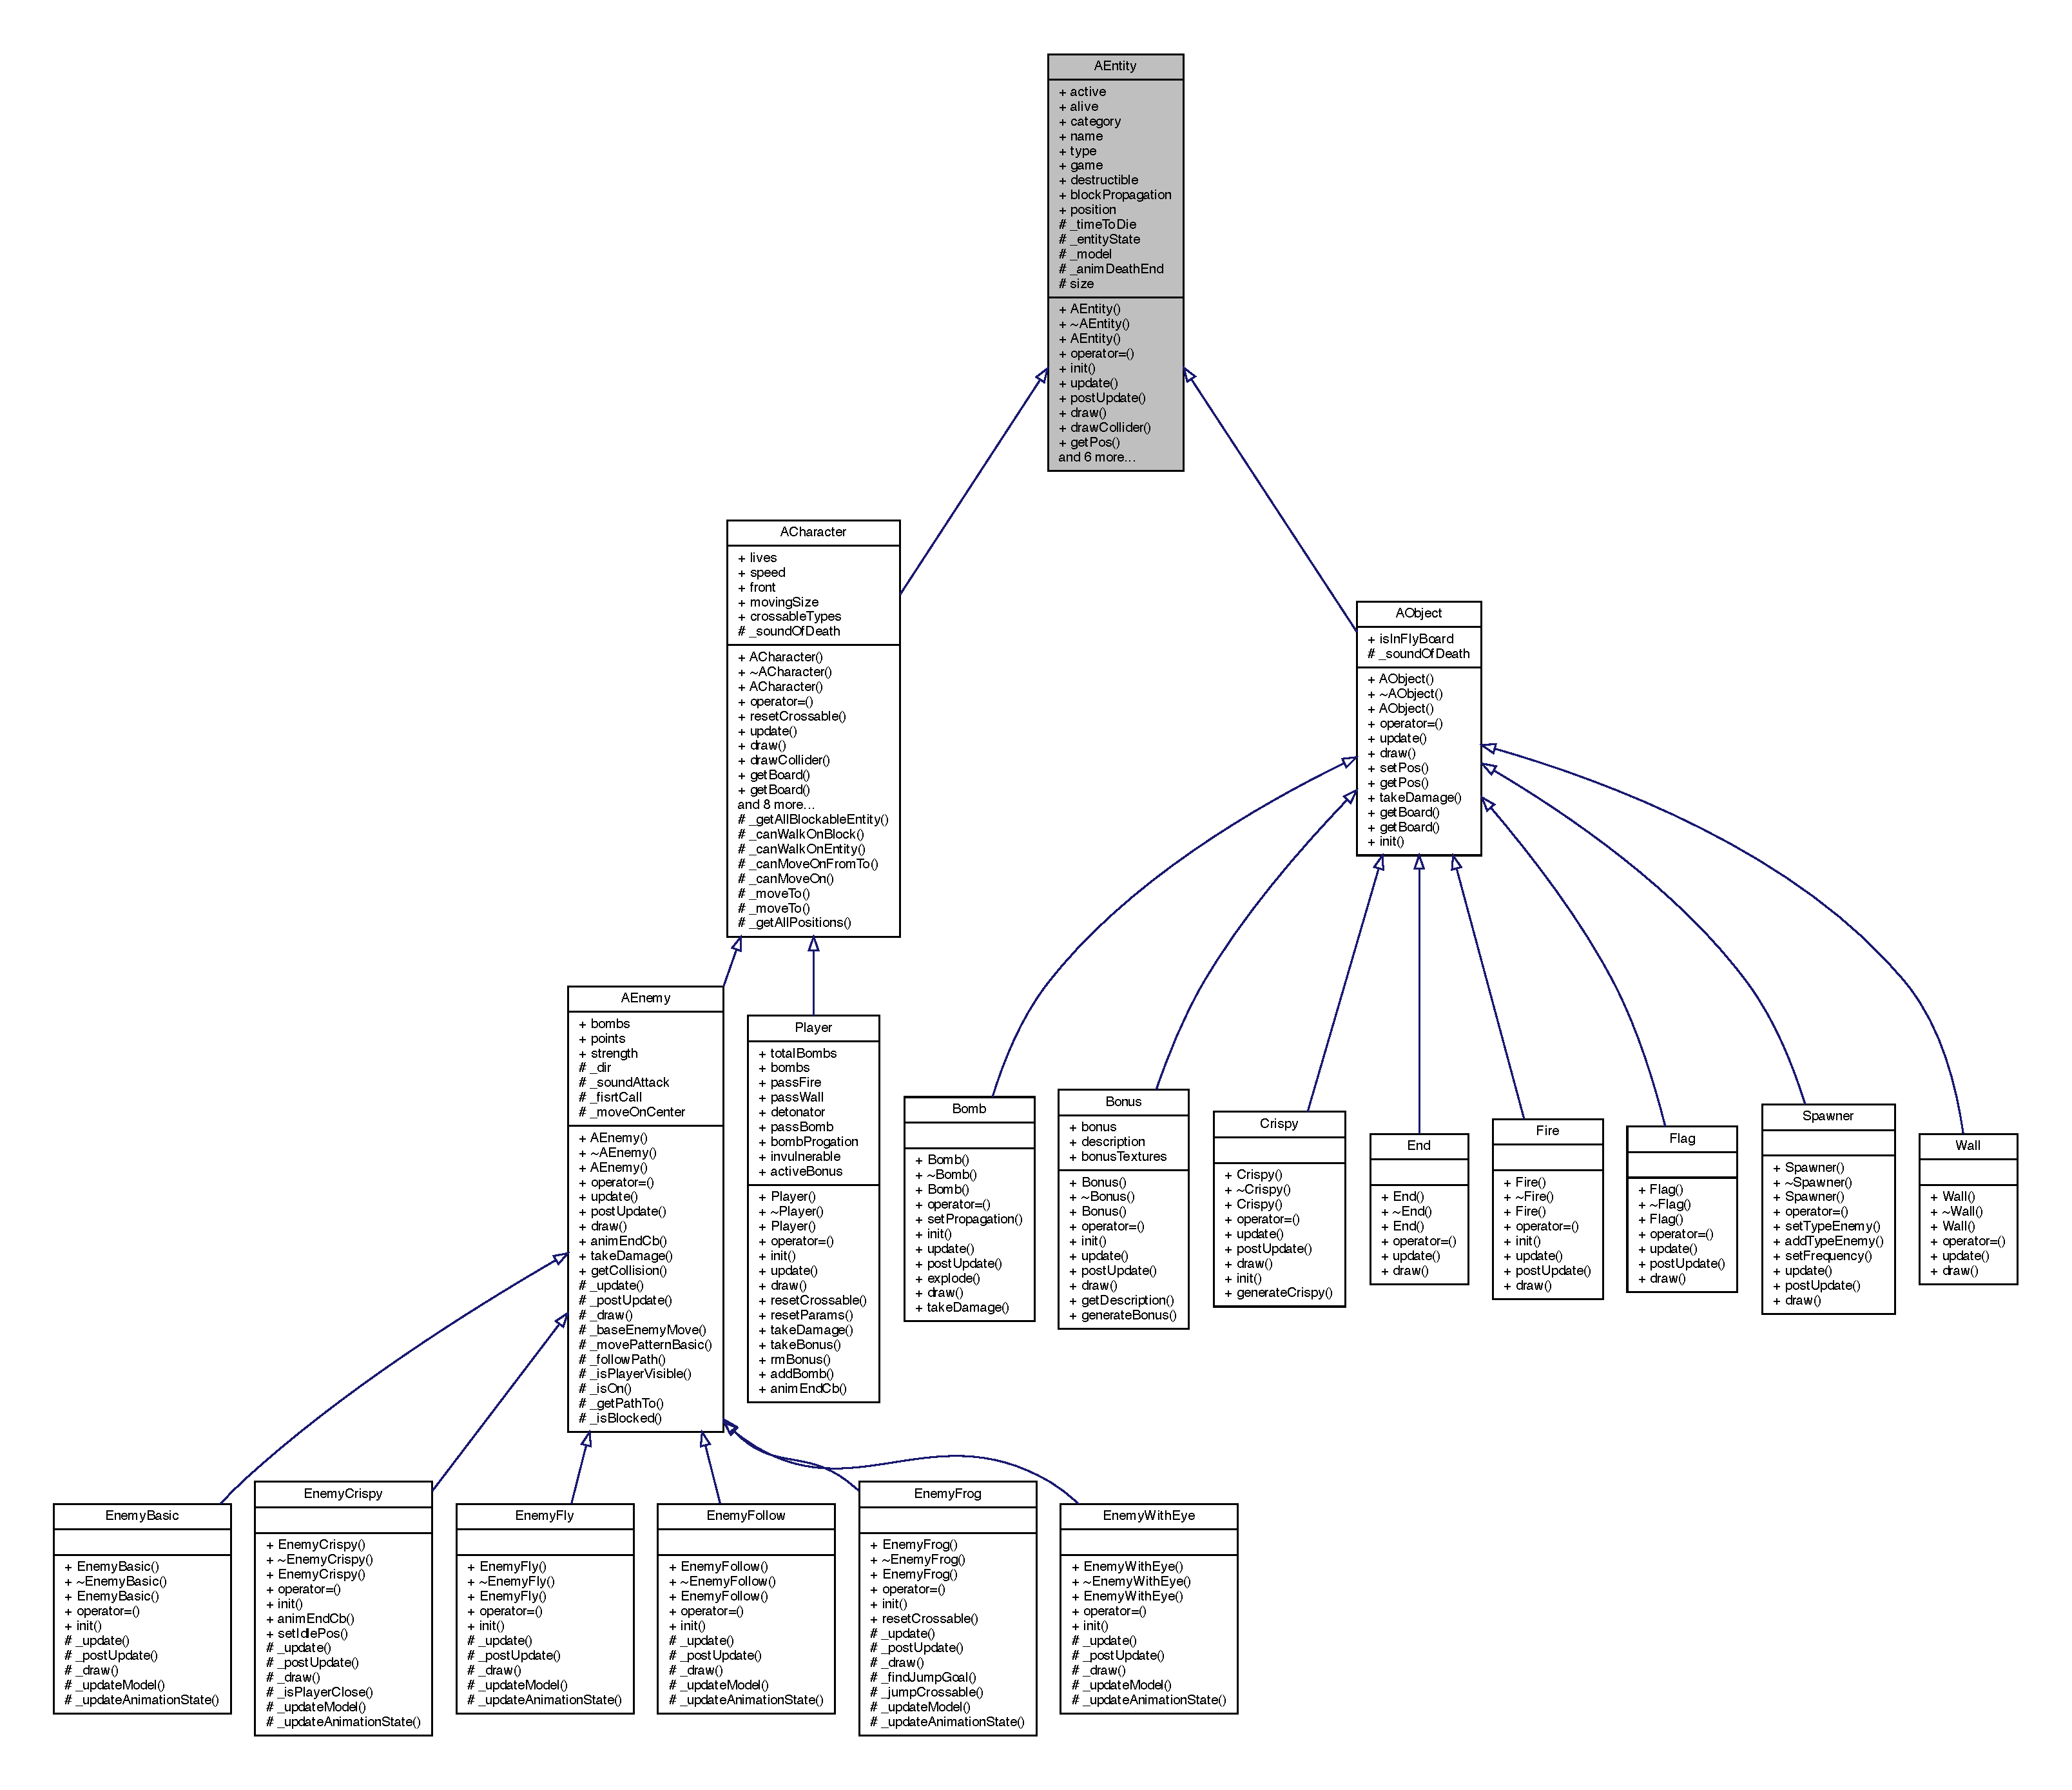
\includegraphics[width=350pt]{class_a_entity__inherit__graph}
\end{center}
\end{figure}


Collaboration diagram for A\+Entity\+:
\nopagebreak
\begin{figure}[H]
\begin{center}
\leavevmode
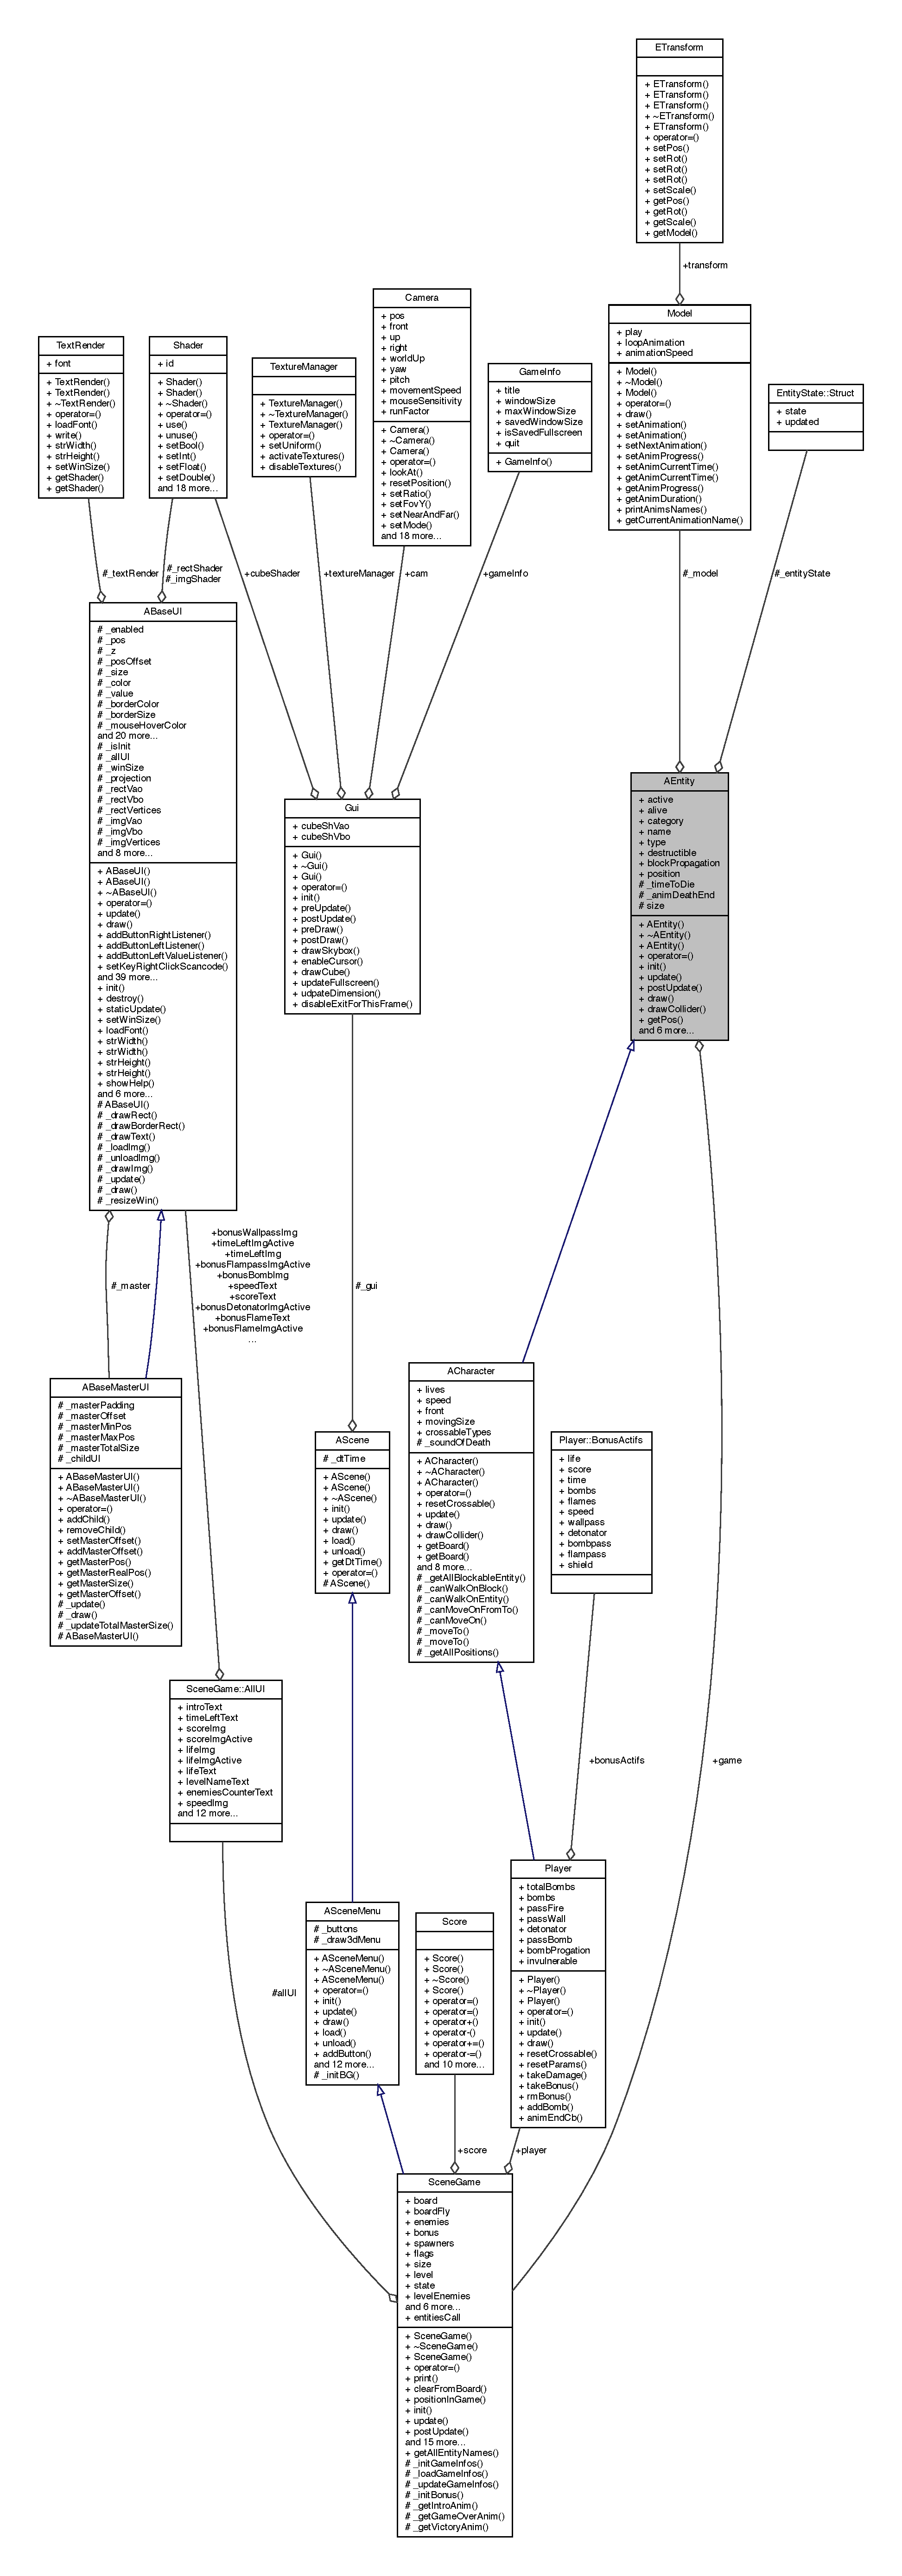
\includegraphics[height=550pt]{class_a_entity__coll__graph}
\end{center}
\end{figure}
\subsection*{Public Member Functions}
\begin{DoxyCompactItemize}
\item 
\hyperlink{class_a_entity_ac2e458e7b02ccd083b2e57c0bb27ea24}{A\+Entity} (\hyperlink{class_scene_game}{Scene\+Game} \&\hyperlink{class_a_entity_aa2c05db944a8b7487eb8470dd20211ab}{game})
\begin{DoxyCompactList}\small\item\em Construct a new A\+Entity\+::\+A\+Entity object. \end{DoxyCompactList}\item 
\mbox{\Hypertarget{class_a_entity_a1680c558ae2cb0d2d65f19147ac857c8}\label{class_a_entity_a1680c558ae2cb0d2d65f19147ac857c8}} 
virtual \hyperlink{class_a_entity_a1680c558ae2cb0d2d65f19147ac857c8}{$\sim$\+A\+Entity} ()
\begin{DoxyCompactList}\small\item\em Destroy the A\+Entity\+::\+A\+Entity object. \end{DoxyCompactList}\item 
\hyperlink{class_a_entity_ad1f884ccc47d377efe359e4fc2ce0592}{A\+Entity} (const \hyperlink{class_a_entity}{A\+Entity} \&src)
\begin{DoxyCompactList}\small\item\em Construct a new A\+Entity\+::\+A\+Entity object. \end{DoxyCompactList}\item 
\hyperlink{class_a_entity}{A\+Entity} \& \hyperlink{class_a_entity_a6eddf1d64b54976fbb9286b477fe19d7}{operator=} (const \hyperlink{class_a_entity}{A\+Entity} \&rhs)
\begin{DoxyCompactList}\small\item\em Overloaded operator. \end{DoxyCompactList}\item 
virtual bool \hyperlink{class_a_entity_a450361b684fa02e4ffe0ba406b8e3b30}{init} ()
\begin{DoxyCompactList}\small\item\em Init method called by load\+Level. \end{DoxyCompactList}\item 
virtual bool \hyperlink{class_a_entity_adcfd3958ca43b8efd7cc58e7106a26a8}{update} ()=0
\begin{DoxyCompactList}\small\item\em Update entity. Called on every frames. \end{DoxyCompactList}\item 
virtual bool \hyperlink{class_a_entity_ae2faa1d11e21033a223fef2bc03b9338}{post\+Update} ()
\begin{DoxyCompactList}\small\item\em Called after update. \end{DoxyCompactList}\item 
virtual bool \hyperlink{class_a_entity_ad9404a7cae108eb81d881d256cacdc12}{draw} (\hyperlink{class_gui}{Gui} \&gui)=0
\begin{DoxyCompactList}\small\item\em Draw entity. Called on every frames. \end{DoxyCompactList}\item 
virtual bool \hyperlink{class_a_entity_aca789d9c82a5fd3da3b196a36e748e8b}{draw\+Collider} ()
\begin{DoxyCompactList}\small\item\em Draw the collider of the entity. \end{DoxyCompactList}\item 
virtual glm\+::vec3 \hyperlink{class_a_entity_afbdb591f06debd7e20e0cb98f14717e4}{get\+Pos} () const =0
\begin{DoxyCompactList}\small\item\em Get the Pos object. \end{DoxyCompactList}\item 
virtual bool \hyperlink{class_a_entity_ac01e24195a8ba249c855120ac017770e}{take\+Damage} (const int damage)=0
\begin{DoxyCompactList}\small\item\em Call this function to take damage. \end{DoxyCompactList}\item 
virtual std\+::vector$<$ std\+::vector$<$ std\+::vector$<$ \hyperlink{class_a_entity}{A\+Entity} $\ast$ $>$ $>$ $>$ const  \& \hyperlink{class_a_entity_a9ed84c8f926cf6032be480ebba7d1820}{get\+Board} () const =0
\begin{DoxyCompactList}\small\item\em Get the Board object. \end{DoxyCompactList}\item 
virtual std\+::vector$<$ std\+::vector$<$ std\+::vector$<$ \hyperlink{class_a_entity}{A\+Entity} $\ast$ $>$ $>$ $>$ \& \hyperlink{class_a_entity_a44aa82958386de50cd9a6c836461114a}{get\+Board} ()=0
\begin{DoxyCompactList}\small\item\em Get the Board object. \end{DoxyCompactList}\item 
virtual void \hyperlink{class_a_entity_ac1fd0bdb4c01a4767660f03cd06cd2ac}{anim\+End\+Cb} (std\+::string anim\+Name)
\begin{DoxyCompactList}\small\item\em called on animation end if passed to \hyperlink{class_model}{Model} need to be redefined by children \end{DoxyCompactList}\item 
void \hyperlink{class_a_entity_ae68a6ff3f5770215116b6ab99d098ed0}{set\+State} (Entity\+State\+::\+Enum state)
\begin{DoxyCompactList}\small\item\em update the entity state \end{DoxyCompactList}\item 
Entity\+State\+::\+Enum \hyperlink{class_a_entity_a135cbfb08a2204ff396de4de2d645b5f}{get\+State} () const
\begin{DoxyCompactList}\small\item\em Get the current animation state. \end{DoxyCompactList}\end{DoxyCompactItemize}
\subsection*{Public Attributes}
\begin{DoxyCompactItemize}
\item 
bool \hyperlink{class_a_entity_a38851d630b58ed997d6c47bc7f2ee58c}{active}
\item 
bool \hyperlink{class_a_entity_a668a6a3428c53d0fd2936a5d59ef52ef}{alive}
\item 
Category\+::\+Enum \hyperlink{class_a_entity_abc6c4a36aeafe9d30a435fbdac516347}{category}
\item 
std\+::string \hyperlink{class_a_entity_a9ebdf8322a0017ff6063f180ef9f037a}{name}
\item 
Type\+::\+Enum \hyperlink{class_a_entity_a4cddb4c9fbae86691e73940edc3731c3}{type}
\item 
\hyperlink{class_scene_game}{Scene\+Game} \& \hyperlink{class_a_entity_aa2c05db944a8b7487eb8470dd20211ab}{game}
\item 
bool \hyperlink{class_a_entity_a09a8ea3c31791230fb95f8c52a12d0b3}{destructible}
\item 
bool \hyperlink{class_a_entity_a0fc8661a7cb58534524e5671e78e7ba1}{block\+Propagation}
\item 
glm\+::vec3 \hyperlink{class_a_entity_acc4f7ad8936089f64c706aa15e86bcea}{position}
\end{DoxyCompactItemize}
\subsection*{Protected Attributes}
\begin{DoxyCompactItemize}
\item 
float \hyperlink{class_a_entity_a771c85ac38a97b2d0772d5bbfa3d8776}{\+\_\+time\+To\+Die}
\item 
\hyperlink{struct_entity_state_1_1_struct}{Entity\+State\+::\+Struct} \hyperlink{class_a_entity_a261052ce4fac95fdba699e7ca48d2dd3}{\+\_\+entity\+State}
\item 
\hyperlink{class_model}{Model} $\ast$ \hyperlink{class_a_entity_abd634d5c2a0be6a6627cade7e4e109d0}{\+\_\+model}
\item 
bool \hyperlink{class_a_entity_a465977aaabcdb73a1b48742897348127}{\+\_\+anim\+Death\+End}
\item 
glm\+::vec3 \hyperlink{class_a_entity_a47f976f25e6214669d64fb2bbb2c455a}{size}
\end{DoxyCompactItemize}


\subsection{Detailed Description}
This is the base class for entity (Charactere, Objects, ...) 

\subsection{Constructor \& Destructor Documentation}
\mbox{\Hypertarget{class_a_entity_ac2e458e7b02ccd083b2e57c0bb27ea24}\label{class_a_entity_ac2e458e7b02ccd083b2e57c0bb27ea24}} 
\index{A\+Entity@{A\+Entity}!A\+Entity@{A\+Entity}}
\index{A\+Entity@{A\+Entity}!A\+Entity@{A\+Entity}}
\subsubsection{\texorpdfstring{A\+Entity()}{AEntity()}\hspace{0.1cm}{\footnotesize\ttfamily [1/2]}}
{\footnotesize\ttfamily A\+Entity\+::\+A\+Entity (\begin{DoxyParamCaption}\item[{\hyperlink{class_scene_game}{Scene\+Game} \&}]{game }\end{DoxyParamCaption})\hspace{0.3cm}{\ttfamily [explicit]}}



Construct a new A\+Entity\+::\+A\+Entity object. 


\begin{DoxyParams}{Parameters}
{\em game} & A reference to the \hyperlink{class_scene_game}{Scene\+Game} object \\
\hline
\end{DoxyParams}
\mbox{\Hypertarget{class_a_entity_ad1f884ccc47d377efe359e4fc2ce0592}\label{class_a_entity_ad1f884ccc47d377efe359e4fc2ce0592}} 
\index{A\+Entity@{A\+Entity}!A\+Entity@{A\+Entity}}
\index{A\+Entity@{A\+Entity}!A\+Entity@{A\+Entity}}
\subsubsection{\texorpdfstring{A\+Entity()}{AEntity()}\hspace{0.1cm}{\footnotesize\ttfamily [2/2]}}
{\footnotesize\ttfamily A\+Entity\+::\+A\+Entity (\begin{DoxyParamCaption}\item[{const \hyperlink{class_a_entity}{A\+Entity} \&}]{src }\end{DoxyParamCaption})}



Construct a new A\+Entity\+::\+A\+Entity object. 


\begin{DoxyParams}{Parameters}
{\em src} & A \hyperlink{class_a_entity}{A\+Entity} element to copy \\
\hline
\end{DoxyParams}


\subsection{Member Function Documentation}
\mbox{\Hypertarget{class_a_entity_ac1fd0bdb4c01a4767660f03cd06cd2ac}\label{class_a_entity_ac1fd0bdb4c01a4767660f03cd06cd2ac}} 
\index{A\+Entity@{A\+Entity}!anim\+End\+Cb@{anim\+End\+Cb}}
\index{anim\+End\+Cb@{anim\+End\+Cb}!A\+Entity@{A\+Entity}}
\subsubsection{\texorpdfstring{anim\+End\+Cb()}{animEndCb()}}
{\footnotesize\ttfamily void A\+Entity\+::anim\+End\+Cb (\begin{DoxyParamCaption}\item[{std\+::string}]{anim\+Name }\end{DoxyParamCaption})\hspace{0.3cm}{\ttfamily [virtual]}}



called on animation end if passed to \hyperlink{class_model}{Model} need to be redefined by children 


\begin{DoxyParams}{Parameters}
{\em anim\+Name} & the current animation name \\
\hline
\end{DoxyParams}


Reimplemented in \hyperlink{class_a_enemy_ac946b6cd7d96f99365301450566d3baf}{A\+Enemy}, \hyperlink{class_player_a26c511cf5a62d7de26347cdc15df609b}{Player}, and \hyperlink{class_enemy_crispy_a32d938b70f4b0f2bd2e1df606c812d13}{Enemy\+Crispy}.

\mbox{\Hypertarget{class_a_entity_ad9404a7cae108eb81d881d256cacdc12}\label{class_a_entity_ad9404a7cae108eb81d881d256cacdc12}} 
\index{A\+Entity@{A\+Entity}!draw@{draw}}
\index{draw@{draw}!A\+Entity@{A\+Entity}}
\subsubsection{\texorpdfstring{draw()}{draw()}}
{\footnotesize\ttfamily virtual bool A\+Entity\+::draw (\begin{DoxyParamCaption}\item[{\hyperlink{class_gui}{Gui} \&}]{gui }\end{DoxyParamCaption})\hspace{0.3cm}{\ttfamily [pure virtual]}}



Draw entity. Called on every frames. 


\begin{DoxyParams}{Parameters}
{\em gui} & A reference to the gui object \\
\hline
\end{DoxyParams}
\begin{DoxyReturn}{Returns}
false If failed 
\end{DoxyReturn}


Implemented in \hyperlink{class_a_enemy_a527fc4b7bb46c04c486fd025a01e16a9}{A\+Enemy}, \hyperlink{class_player_a1194c157df144e864d0328d267dfa75c}{Player}, \hyperlink{class_a_character_af223d3c9dbd3143daf62e9834bd30e3d}{A\+Character}, \hyperlink{class_bonus_acdb40deca7be37984084fb3d4fef85ed}{Bonus}, \hyperlink{class_spawner_a1532fd875b6a3aacb617b1111b818f01}{Spawner}, \hyperlink{class_bomb_ae0ea4aa0ce14d353ad63c31cccc2a69d}{Bomb}, \hyperlink{class_a_object_a5e454e13e04ee937c20a465244cf748a}{A\+Object}, \hyperlink{class_end_aad5c7ef71927eddfd634e0a0879cb99a}{End}, \hyperlink{class_crispy_a266bebd70e55a7d08ba1688af0f4adf0}{Crispy}, \hyperlink{class_wall_ab3ea42b91f7830d22782901d61be505f}{Wall}, \hyperlink{class_flag_ae24cc9c0e3cc3378e12af9f40c0ee93d}{Flag}, and \hyperlink{class_fire_a622efdbee6254c463250b6d9033428eb}{Fire}.

\mbox{\Hypertarget{class_a_entity_aca789d9c82a5fd3da3b196a36e748e8b}\label{class_a_entity_aca789d9c82a5fd3da3b196a36e748e8b}} 
\index{A\+Entity@{A\+Entity}!draw\+Collider@{draw\+Collider}}
\index{draw\+Collider@{draw\+Collider}!A\+Entity@{A\+Entity}}
\subsubsection{\texorpdfstring{draw\+Collider()}{drawCollider()}}
{\footnotesize\ttfamily bool A\+Entity\+::draw\+Collider (\begin{DoxyParamCaption}{ }\end{DoxyParamCaption})\hspace{0.3cm}{\ttfamily [virtual]}}



Draw the collider of the entity. 

\begin{DoxyReturn}{Returns}
false If failed 
\end{DoxyReturn}


Reimplemented in \hyperlink{class_a_character_a2cc5faf1d9047d9e51154d5663fa6c67}{A\+Character}.

\mbox{\Hypertarget{class_a_entity_a9ed84c8f926cf6032be480ebba7d1820}\label{class_a_entity_a9ed84c8f926cf6032be480ebba7d1820}} 
\index{A\+Entity@{A\+Entity}!get\+Board@{get\+Board}}
\index{get\+Board@{get\+Board}!A\+Entity@{A\+Entity}}
\subsubsection{\texorpdfstring{get\+Board()}{getBoard()}\hspace{0.1cm}{\footnotesize\ttfamily [1/2]}}
{\footnotesize\ttfamily virtual std\+::vector$<$ std\+::vector$<$ std\+::vector$<$\hyperlink{class_a_entity}{A\+Entity} $\ast$$>$ $>$ $>$ const\& A\+Entity\+::get\+Board (\begin{DoxyParamCaption}{ }\end{DoxyParamCaption}) const\hspace{0.3cm}{\ttfamily [pure virtual]}}



Get the Board object. 

\begin{DoxyReturn}{Returns}
std\+::vector$<$ std\+::vector$<$ std\+::vector$<$\+A\+Entity $\ast$$>$ $>$ $>$ const\& The board object 
\end{DoxyReturn}


Implemented in \hyperlink{class_a_character_adecb8064d5070f15a2d6aa76a151ff33}{A\+Character}, and \hyperlink{class_a_object_ac4a82eef484c0f7bf3547a7f7f6dce7e}{A\+Object}.

\mbox{\Hypertarget{class_a_entity_a44aa82958386de50cd9a6c836461114a}\label{class_a_entity_a44aa82958386de50cd9a6c836461114a}} 
\index{A\+Entity@{A\+Entity}!get\+Board@{get\+Board}}
\index{get\+Board@{get\+Board}!A\+Entity@{A\+Entity}}
\subsubsection{\texorpdfstring{get\+Board()}{getBoard()}\hspace{0.1cm}{\footnotesize\ttfamily [2/2]}}
{\footnotesize\ttfamily virtual std\+::vector$<$ std\+::vector$<$ std\+::vector$<$\hyperlink{class_a_entity}{A\+Entity} $\ast$$>$ $>$ $>$\& A\+Entity\+::get\+Board (\begin{DoxyParamCaption}{ }\end{DoxyParamCaption})\hspace{0.3cm}{\ttfamily [pure virtual]}}



Get the Board object. 

\begin{DoxyReturn}{Returns}
std\+::vector$<$ std\+::vector$<$ std\+::vector$<$\+A\+Entity $\ast$$>$ $>$ $>$ const\& The board object 
\end{DoxyReturn}


Implemented in \hyperlink{class_a_character_aa8f0b9b557c69eead696870c41c8321b}{A\+Character}, and \hyperlink{class_a_object_aba4b07c0456b2c3d42a71529ef40f2d5}{A\+Object}.

\mbox{\Hypertarget{class_a_entity_afbdb591f06debd7e20e0cb98f14717e4}\label{class_a_entity_afbdb591f06debd7e20e0cb98f14717e4}} 
\index{A\+Entity@{A\+Entity}!get\+Pos@{get\+Pos}}
\index{get\+Pos@{get\+Pos}!A\+Entity@{A\+Entity}}
\subsubsection{\texorpdfstring{get\+Pos()}{getPos()}}
{\footnotesize\ttfamily virtual glm\+::vec3 A\+Entity\+::get\+Pos (\begin{DoxyParamCaption}{ }\end{DoxyParamCaption}) const\hspace{0.3cm}{\ttfamily [pure virtual]}}



Get the Pos object. 

\begin{DoxyReturn}{Returns}
glm\+::vec3 The position 
\end{DoxyReturn}


Implemented in \hyperlink{class_a_character_a41875fc55beaafd65fbe53ea3abc7f98}{A\+Character}, and \hyperlink{class_a_object_ab5840de6100bba8bf93a186a0a802708}{A\+Object}.

\mbox{\Hypertarget{class_a_entity_a135cbfb08a2204ff396de4de2d645b5f}\label{class_a_entity_a135cbfb08a2204ff396de4de2d645b5f}} 
\index{A\+Entity@{A\+Entity}!get\+State@{get\+State}}
\index{get\+State@{get\+State}!A\+Entity@{A\+Entity}}
\subsubsection{\texorpdfstring{get\+State()}{getState()}}
{\footnotesize\ttfamily Entity\+State\+::\+Enum A\+Entity\+::get\+State (\begin{DoxyParamCaption}{ }\end{DoxyParamCaption}) const}



Get the current animation state. 

\begin{DoxyReturn}{Returns}
Entity\+State\+::\+Enum The state 
\end{DoxyReturn}
\mbox{\Hypertarget{class_a_entity_a450361b684fa02e4ffe0ba406b8e3b30}\label{class_a_entity_a450361b684fa02e4ffe0ba406b8e3b30}} 
\index{A\+Entity@{A\+Entity}!init@{init}}
\index{init@{init}!A\+Entity@{A\+Entity}}
\subsubsection{\texorpdfstring{init()}{init()}}
{\footnotesize\ttfamily bool A\+Entity\+::init (\begin{DoxyParamCaption}{ }\end{DoxyParamCaption})\hspace{0.3cm}{\ttfamily [virtual]}}



Init method called by load\+Level. 

\begin{DoxyReturn}{Returns}
true on success 

false on failure 
\end{DoxyReturn}


Reimplemented in \hyperlink{class_player_afcf86538719baa2f5c81d0b90263c41a}{Player}, \hyperlink{class_bonus_a976414b70e76b18dadeae3f316a22547}{Bonus}, \hyperlink{class_enemy_frog_adb2293192dd66ee46da359833475915b}{Enemy\+Frog}, \hyperlink{class_a_object_afa83ef1c900a47453524219788327b86}{A\+Object}, \hyperlink{class_enemy_follow_a09963fbac6d395dbf653b6353412cf2b}{Enemy\+Follow}, \hyperlink{class_enemy_crispy_a87a926e52fd94e7307baaad8cb1b4977}{Enemy\+Crispy}, \hyperlink{class_spawner_a274d6abcfeb55784de07f3c36ae923ce}{Spawner}, \hyperlink{class_enemy_with_eye_afe1006e6d3cdba1365bbc29fcc9f71b0}{Enemy\+With\+Eye}, \hyperlink{class_enemy_fly_a8957442e19b91b06bf1f3bb650d66a8c}{Enemy\+Fly}, \hyperlink{class_enemy_basic_a898943e397eb36c80721951a3457178c}{Enemy\+Basic}, \hyperlink{class_end_a1c57c2279d61916ea97aed566e8b3663}{End}, \hyperlink{class_bomb_a4a3f751937f59953f4cf585b07c9684c}{Bomb}, \hyperlink{class_crispy_aef91bfa94d0506d25b4cf78098e57912}{Crispy}, \hyperlink{class_flag_abdb7a9ef47dd6ea6a24beec99b372f11}{Flag}, and \hyperlink{class_fire_ae6456b9911e675ed1fb030f5f9e89cc8}{Fire}.

\mbox{\Hypertarget{class_a_entity_a6eddf1d64b54976fbb9286b477fe19d7}\label{class_a_entity_a6eddf1d64b54976fbb9286b477fe19d7}} 
\index{A\+Entity@{A\+Entity}!operator=@{operator=}}
\index{operator=@{operator=}!A\+Entity@{A\+Entity}}
\subsubsection{\texorpdfstring{operator=()}{operator=()}}
{\footnotesize\ttfamily \hyperlink{class_a_entity}{A\+Entity} \& A\+Entity\+::operator= (\begin{DoxyParamCaption}\item[{const \hyperlink{class_a_entity}{A\+Entity} \&}]{rhs }\end{DoxyParamCaption})}



Overloaded operator. 


\begin{DoxyParams}{Parameters}
{\em rhs} & Right element \\
\hline
\end{DoxyParams}
\begin{DoxyReturn}{Returns}
\hyperlink{class_a_entity}{A\+Entity}\& A ref to a new object 
\end{DoxyReturn}
\mbox{\Hypertarget{class_a_entity_ae2faa1d11e21033a223fef2bc03b9338}\label{class_a_entity_ae2faa1d11e21033a223fef2bc03b9338}} 
\index{A\+Entity@{A\+Entity}!post\+Update@{post\+Update}}
\index{post\+Update@{post\+Update}!A\+Entity@{A\+Entity}}
\subsubsection{\texorpdfstring{post\+Update()}{postUpdate()}}
{\footnotesize\ttfamily bool A\+Entity\+::post\+Update (\begin{DoxyParamCaption}{ }\end{DoxyParamCaption})\hspace{0.3cm}{\ttfamily [virtual]}}



Called after update. 

\begin{DoxyReturn}{Returns}
false If failed 
\end{DoxyReturn}


Reimplemented in \hyperlink{class_a_enemy_a2d2ff5a126f14294bdbc17475c363d00}{A\+Enemy}, \hyperlink{class_bonus_a6524cf732f98dfc3baa7f41bbdf13b11}{Bonus}, \hyperlink{class_spawner_ab8a55710ca6e122d975f697a9c7643bc}{Spawner}, \hyperlink{class_bomb_a443c5d40a92e67ef456c71369e8a111b}{Bomb}, \hyperlink{class_crispy_aa83ad22c80b962ee0380c1e394ae8610}{Crispy}, \hyperlink{class_flag_a1840a0949762e3e62bf156be6e173d1e}{Flag}, and \hyperlink{class_fire_adba3c7ec49ed7d31fd35250105a35edf}{Fire}.

\mbox{\Hypertarget{class_a_entity_ae68a6ff3f5770215116b6ab99d098ed0}\label{class_a_entity_ae68a6ff3f5770215116b6ab99d098ed0}} 
\index{A\+Entity@{A\+Entity}!set\+State@{set\+State}}
\index{set\+State@{set\+State}!A\+Entity@{A\+Entity}}
\subsubsection{\texorpdfstring{set\+State()}{setState()}}
{\footnotesize\ttfamily void A\+Entity\+::set\+State (\begin{DoxyParamCaption}\item[{Entity\+State\+::\+Enum}]{state }\end{DoxyParamCaption})}



update the entity state 


\begin{DoxyParams}{Parameters}
{\em state} & the new state \\
\hline
\end{DoxyParams}
\mbox{\Hypertarget{class_a_entity_ac01e24195a8ba249c855120ac017770e}\label{class_a_entity_ac01e24195a8ba249c855120ac017770e}} 
\index{A\+Entity@{A\+Entity}!take\+Damage@{take\+Damage}}
\index{take\+Damage@{take\+Damage}!A\+Entity@{A\+Entity}}
\subsubsection{\texorpdfstring{take\+Damage()}{takeDamage()}}
{\footnotesize\ttfamily virtual bool A\+Entity\+::take\+Damage (\begin{DoxyParamCaption}\item[{const int}]{damage }\end{DoxyParamCaption})\hspace{0.3cm}{\ttfamily [pure virtual]}}



Call this function to take damage. 


\begin{DoxyParams}{Parameters}
{\em damage} & Number of damage taken \\
\hline
\end{DoxyParams}
\begin{DoxyReturn}{Returns}
false If not active or indestructible 
\end{DoxyReturn}


Implemented in \hyperlink{class_a_enemy_a17bcf116c42c3d780e243127adf1a947}{A\+Enemy}, \hyperlink{class_player_a029b1d511340697d8ccfb7bfa604435b}{Player}, \hyperlink{class_a_character_a1ab94580e4db621f79f0bf1d6bcdb600}{A\+Character}, \hyperlink{class_a_object_a39b1720ae5a820512ab4db0906f03b15}{A\+Object}, and \hyperlink{class_bomb_ac51b260cdfef0cde903a88003994276e}{Bomb}.

\mbox{\Hypertarget{class_a_entity_adcfd3958ca43b8efd7cc58e7106a26a8}\label{class_a_entity_adcfd3958ca43b8efd7cc58e7106a26a8}} 
\index{A\+Entity@{A\+Entity}!update@{update}}
\index{update@{update}!A\+Entity@{A\+Entity}}
\subsubsection{\texorpdfstring{update()}{update()}}
{\footnotesize\ttfamily virtual bool A\+Entity\+::update (\begin{DoxyParamCaption}{ }\end{DoxyParamCaption})\hspace{0.3cm}{\ttfamily [pure virtual]}}



Update entity. Called on every frames. 

\begin{DoxyReturn}{Returns}
false If failed 
\end{DoxyReturn}


Implemented in \hyperlink{class_a_enemy_a01e3b0313d6f29bf2cafe20f711c0550}{A\+Enemy}, \hyperlink{class_player_a1614c89caa50fa1527417ba6a2bbe6ee}{Player}, \hyperlink{class_a_character_af5a4d00f6104d45b821a2e88b80936b5}{A\+Character}, \hyperlink{class_bonus_a0dd8aa4474c3d1ef494ed8a916cc16cd}{Bonus}, \hyperlink{class_spawner_a9325e76299405d5d74abfb72f4ea2380}{Spawner}, \hyperlink{class_end_a7154532cce1c86f4f5bfa98eb0c25574}{End}, \hyperlink{class_bomb_a9808d8efcc57b9ce7b0bd48d95875aad}{Bomb}, \hyperlink{class_a_object_af35bb4b68af0a11bb1fcf617bde41ecd}{A\+Object}, \hyperlink{class_wall_a29d3c4daa11dbb20d758b1fc285ed7a4}{Wall}, \hyperlink{class_crispy_ab33c8c68fa636df5721581e8f68ceae3}{Crispy}, \hyperlink{class_flag_adeaab6cd88bbc3284f8b4f1b2f78242b}{Flag}, and \hyperlink{class_fire_a86114cf78108a4b202b75e1f383b3e00}{Fire}.



\subsection{Member Data Documentation}
\mbox{\Hypertarget{class_a_entity_a465977aaabcdb73a1b48742897348127}\label{class_a_entity_a465977aaabcdb73a1b48742897348127}} 
\index{A\+Entity@{A\+Entity}!\+\_\+anim\+Death\+End@{\+\_\+anim\+Death\+End}}
\index{\+\_\+anim\+Death\+End@{\+\_\+anim\+Death\+End}!A\+Entity@{A\+Entity}}
\subsubsection{\texorpdfstring{\+\_\+anim\+Death\+End}{\_animDeathEnd}}
{\footnotesize\ttfamily bool A\+Entity\+::\+\_\+anim\+Death\+End\hspace{0.3cm}{\ttfamily [protected]}}

True if the entity has a death animation \mbox{\Hypertarget{class_a_entity_a261052ce4fac95fdba699e7ca48d2dd3}\label{class_a_entity_a261052ce4fac95fdba699e7ca48d2dd3}} 
\index{A\+Entity@{A\+Entity}!\+\_\+entity\+State@{\+\_\+entity\+State}}
\index{\+\_\+entity\+State@{\+\_\+entity\+State}!A\+Entity@{A\+Entity}}
\subsubsection{\texorpdfstring{\+\_\+entity\+State}{\_entityState}}
{\footnotesize\ttfamily \hyperlink{struct_entity_state_1_1_struct}{Entity\+State\+::\+Struct} A\+Entity\+::\+\_\+entity\+State\hspace{0.3cm}{\ttfamily [protected]}}

The entity state (current animation\+: run, idle, ...) \mbox{\Hypertarget{class_a_entity_abd634d5c2a0be6a6627cade7e4e109d0}\label{class_a_entity_abd634d5c2a0be6a6627cade7e4e109d0}} 
\index{A\+Entity@{A\+Entity}!\+\_\+model@{\+\_\+model}}
\index{\+\_\+model@{\+\_\+model}!A\+Entity@{A\+Entity}}
\subsubsection{\texorpdfstring{\+\_\+model}{\_model}}
{\footnotesize\ttfamily \hyperlink{class_model}{Model}$\ast$ A\+Entity\+::\+\_\+model\hspace{0.3cm}{\ttfamily [protected]}}

The 3D model of the entity \mbox{\Hypertarget{class_a_entity_a771c85ac38a97b2d0772d5bbfa3d8776}\label{class_a_entity_a771c85ac38a97b2d0772d5bbfa3d8776}} 
\index{A\+Entity@{A\+Entity}!\+\_\+time\+To\+Die@{\+\_\+time\+To\+Die}}
\index{\+\_\+time\+To\+Die@{\+\_\+time\+To\+Die}!A\+Entity@{A\+Entity}}
\subsubsection{\texorpdfstring{\+\_\+time\+To\+Die}{\_timeToDie}}
{\footnotesize\ttfamily float A\+Entity\+::\+\_\+time\+To\+Die\hspace{0.3cm}{\ttfamily [protected]}}

The time to die (animation) \mbox{\Hypertarget{class_a_entity_a38851d630b58ed997d6c47bc7f2ee58c}\label{class_a_entity_a38851d630b58ed997d6c47bc7f2ee58c}} 
\index{A\+Entity@{A\+Entity}!active@{active}}
\index{active@{active}!A\+Entity@{A\+Entity}}
\subsubsection{\texorpdfstring{active}{active}}
{\footnotesize\ttfamily bool A\+Entity\+::active}

True if the entity is active \mbox{\Hypertarget{class_a_entity_a668a6a3428c53d0fd2936a5d59ef52ef}\label{class_a_entity_a668a6a3428c53d0fd2936a5d59ef52ef}} 
\index{A\+Entity@{A\+Entity}!alive@{alive}}
\index{alive@{alive}!A\+Entity@{A\+Entity}}
\subsubsection{\texorpdfstring{alive}{alive}}
{\footnotesize\ttfamily bool A\+Entity\+::alive}

True if the entity is alive \mbox{\Hypertarget{class_a_entity_a0fc8661a7cb58534524e5671e78e7ba1}\label{class_a_entity_a0fc8661a7cb58534524e5671e78e7ba1}} 
\index{A\+Entity@{A\+Entity}!block\+Propagation@{block\+Propagation}}
\index{block\+Propagation@{block\+Propagation}!A\+Entity@{A\+Entity}}
\subsubsection{\texorpdfstring{block\+Propagation}{blockPropagation}}
{\footnotesize\ttfamily bool A\+Entity\+::block\+Propagation}

Used in bombs for explosion propagation \mbox{\Hypertarget{class_a_entity_abc6c4a36aeafe9d30a435fbdac516347}\label{class_a_entity_abc6c4a36aeafe9d30a435fbdac516347}} 
\index{A\+Entity@{A\+Entity}!category@{category}}
\index{category@{category}!A\+Entity@{A\+Entity}}
\subsubsection{\texorpdfstring{category}{category}}
{\footnotesize\ttfamily Category\+::\+Enum A\+Entity\+::category}

The entity category (Category\+::\+S\+T\+A\+T\+IC $\vert$ Category\+::\+M\+O\+B\+I\+LE) \mbox{\Hypertarget{class_a_entity_a09a8ea3c31791230fb95f8c52a12d0b3}\label{class_a_entity_a09a8ea3c31791230fb95f8c52a12d0b3}} 
\index{A\+Entity@{A\+Entity}!destructible@{destructible}}
\index{destructible@{destructible}!A\+Entity@{A\+Entity}}
\subsubsection{\texorpdfstring{destructible}{destructible}}
{\footnotesize\ttfamily bool A\+Entity\+::destructible}

True if the entity is destructible (by bombs) \mbox{\Hypertarget{class_a_entity_aa2c05db944a8b7487eb8470dd20211ab}\label{class_a_entity_aa2c05db944a8b7487eb8470dd20211ab}} 
\index{A\+Entity@{A\+Entity}!game@{game}}
\index{game@{game}!A\+Entity@{A\+Entity}}
\subsubsection{\texorpdfstring{game}{game}}
{\footnotesize\ttfamily \hyperlink{class_scene_game}{Scene\+Game}\& A\+Entity\+::game}

A reference to the main scene for game \mbox{\Hypertarget{class_a_entity_a9ebdf8322a0017ff6063f180ef9f037a}\label{class_a_entity_a9ebdf8322a0017ff6063f180ef9f037a}} 
\index{A\+Entity@{A\+Entity}!name@{name}}
\index{name@{name}!A\+Entity@{A\+Entity}}
\subsubsection{\texorpdfstring{name}{name}}
{\footnotesize\ttfamily std\+::string A\+Entity\+::name}

The entity name \mbox{\Hypertarget{class_a_entity_acc4f7ad8936089f64c706aa15e86bcea}\label{class_a_entity_acc4f7ad8936089f64c706aa15e86bcea}} 
\index{A\+Entity@{A\+Entity}!position@{position}}
\index{position@{position}!A\+Entity@{A\+Entity}}
\subsubsection{\texorpdfstring{position}{position}}
{\footnotesize\ttfamily glm\+::vec3 A\+Entity\+::position}

The entity position \mbox{\Hypertarget{class_a_entity_a47f976f25e6214669d64fb2bbb2c455a}\label{class_a_entity_a47f976f25e6214669d64fb2bbb2c455a}} 
\index{A\+Entity@{A\+Entity}!size@{size}}
\index{size@{size}!A\+Entity@{A\+Entity}}
\subsubsection{\texorpdfstring{size}{size}}
{\footnotesize\ttfamily glm\+::vec3 A\+Entity\+::size\hspace{0.3cm}{\ttfamily [protected]}}

The entity size \mbox{\Hypertarget{class_a_entity_a4cddb4c9fbae86691e73940edc3731c3}\label{class_a_entity_a4cddb4c9fbae86691e73940edc3731c3}} 
\index{A\+Entity@{A\+Entity}!type@{type}}
\index{type@{type}!A\+Entity@{A\+Entity}}
\subsubsection{\texorpdfstring{type}{type}}
{\footnotesize\ttfamily Type\+::\+Enum A\+Entity\+::type}

The entity type 

The documentation for this class was generated from the following files\+:\begin{DoxyCompactItemize}
\item 
includes/A\+Entity.\+hpp\item 
srcs/A\+Entity.\+cpp\end{DoxyCompactItemize}

\hypertarget{struct_scene_end_game_1_1_all_u_i}{}\doxysection{Scene\+End\+Game\+::All\+UI Struct Reference}
\label{struct_scene_end_game_1_1_all_u_i}\index{SceneEndGame::AllUI@{SceneEndGame::AllUI}}


Collaboration diagram for Scene\+End\+Game\+::All\+UI\+:
\nopagebreak
\begin{figure}[H]
\begin{center}
\leavevmode
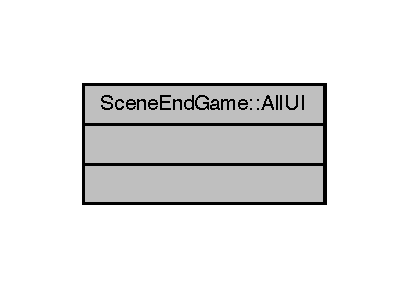
\includegraphics[width=196pt]{struct_scene_end_game_1_1_all_u_i__coll__graph}
\end{center}
\end{figure}


The documentation for this struct was generated from the following file\+:\begin{DoxyCompactItemize}
\item 
includes/scenes/Scene\+End\+Game.\+hpp\end{DoxyCompactItemize}

\hypertarget{struct_scene_exit_1_1_all_u_i}{}\doxysection{Scene\+Exit\+::All\+UI Struct Reference}
\label{struct_scene_exit_1_1_all_u_i}\index{SceneExit::AllUI@{SceneExit::AllUI}}


Collaboration diagram for Scene\+Exit\+::All\+UI\+:
\nopagebreak
\begin{figure}[H]
\begin{center}
\leavevmode
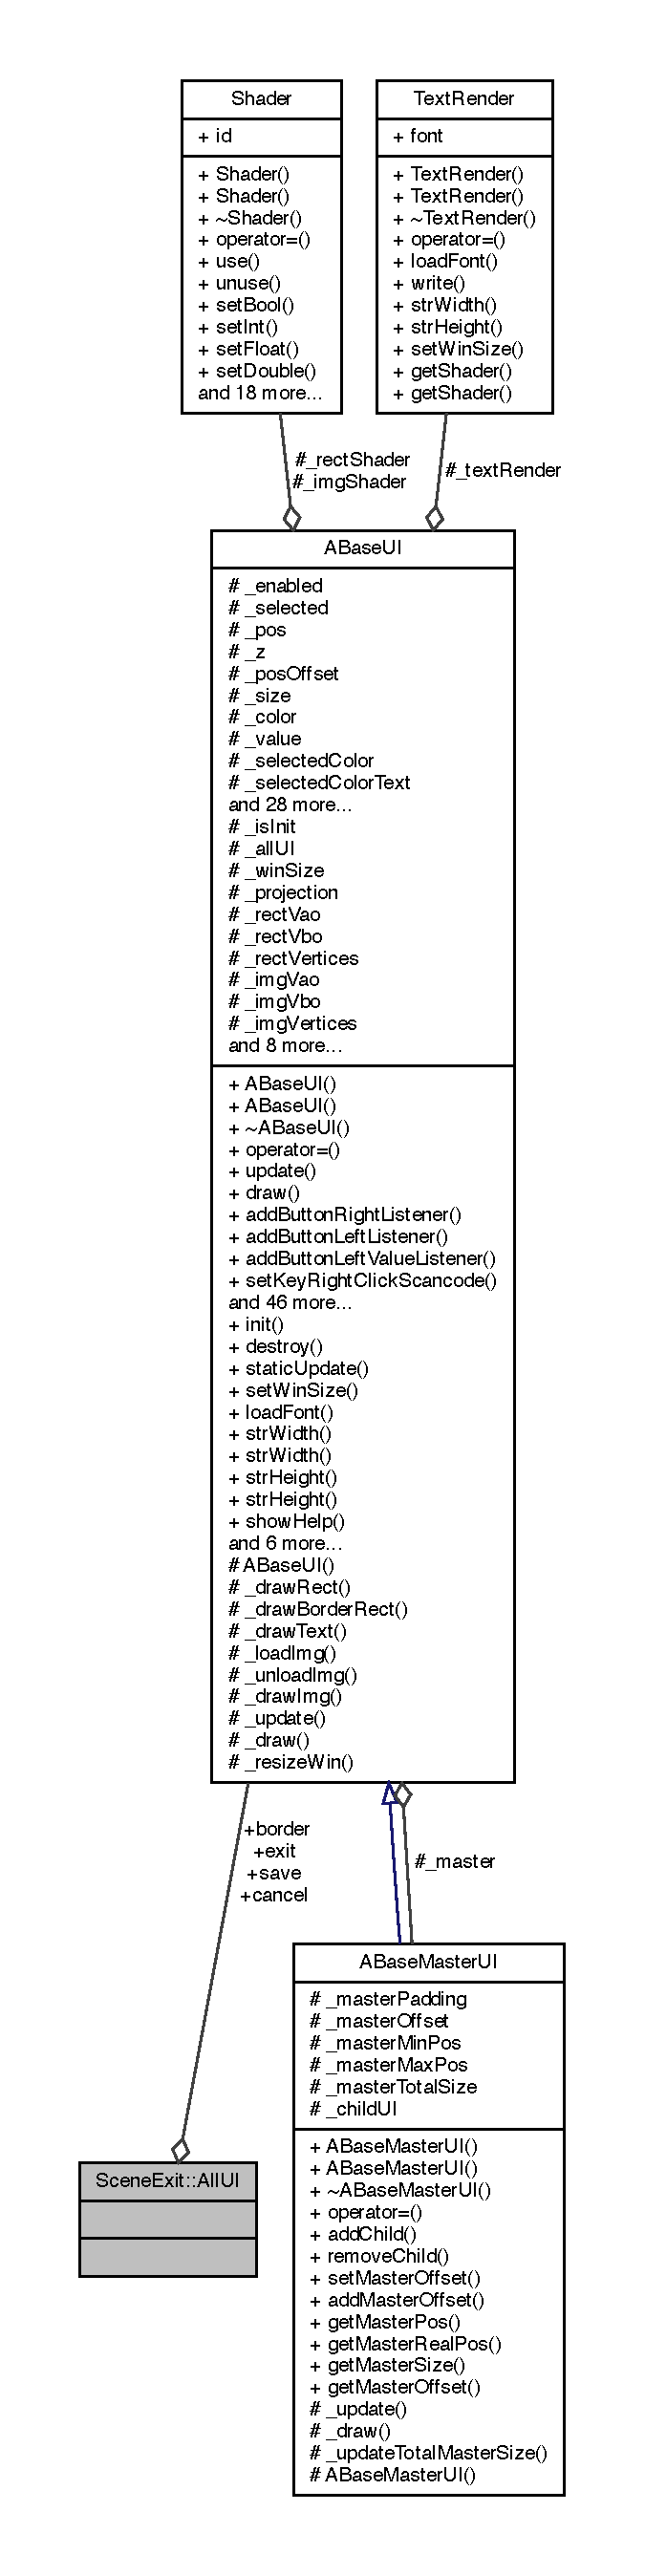
\includegraphics[height=550pt]{struct_scene_exit_1_1_all_u_i__coll__graph}
\end{center}
\end{figure}
\doxysubsection*{Public Attributes}
\begin{DoxyCompactItemize}
\item 
\mbox{\Hypertarget{struct_scene_exit_1_1_all_u_i_ac32d7e8963242711eced6bdcc72a7d07}\label{struct_scene_exit_1_1_all_u_i_ac32d7e8963242711eced6bdcc72a7d07}} 
\mbox{\hyperlink{class_a_base_u_i}{A\+Base\+UI}} $\ast$ {\bfseries exit}
\item 
\mbox{\Hypertarget{struct_scene_exit_1_1_all_u_i_a1792ebe1f40975e5e0d5613d844939eb}\label{struct_scene_exit_1_1_all_u_i_a1792ebe1f40975e5e0d5613d844939eb}} 
\mbox{\hyperlink{class_a_base_u_i}{A\+Base\+UI}} $\ast$ {\bfseries cancel}
\item 
\mbox{\Hypertarget{struct_scene_exit_1_1_all_u_i_abc6ec694aeb6052218b97382aae13af1}\label{struct_scene_exit_1_1_all_u_i_abc6ec694aeb6052218b97382aae13af1}} 
\mbox{\hyperlink{class_a_base_u_i}{A\+Base\+UI}} $\ast$ {\bfseries save}
\item 
\mbox{\Hypertarget{struct_scene_exit_1_1_all_u_i_a92131df68b23377e1856254b00ea6c51}\label{struct_scene_exit_1_1_all_u_i_a92131df68b23377e1856254b00ea6c51}} 
\mbox{\hyperlink{class_a_base_u_i}{A\+Base\+UI}} $\ast$ {\bfseries border}
\end{DoxyCompactItemize}


The documentation for this struct was generated from the following file\+:\begin{DoxyCompactItemize}
\item 
includes/scenes/Scene\+Exit.\+hpp\end{DoxyCompactItemize}

\hypertarget{struct_scene_game_1_1_all_u_i}{}\doxysection{Scene\+Game\+::All\+UI Struct Reference}
\label{struct_scene_game_1_1_all_u_i}\index{SceneGame::AllUI@{SceneGame::AllUI}}


Collaboration diagram for Scene\+Game\+::All\+UI\+:
\nopagebreak
\begin{figure}[H]
\begin{center}
\leavevmode
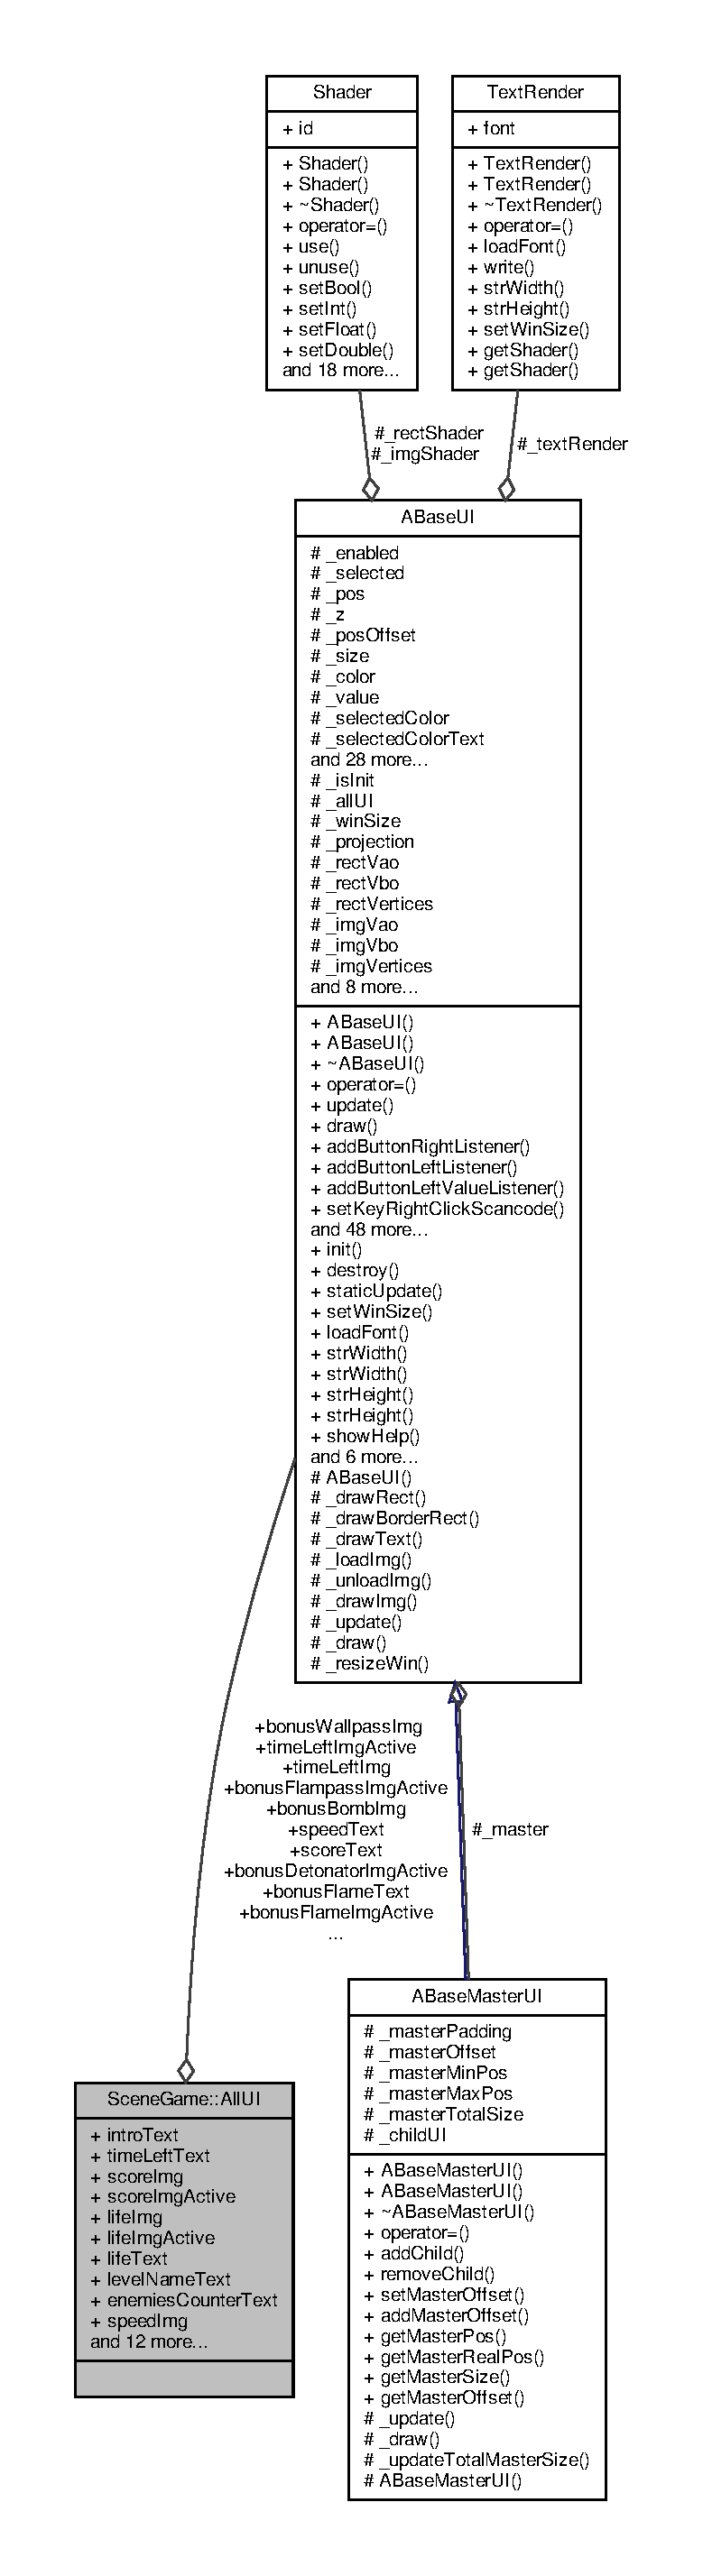
\includegraphics[height=550pt]{struct_scene_game_1_1_all_u_i__coll__graph}
\end{center}
\end{figure}
\doxysubsection*{Public Attributes}
\begin{DoxyCompactItemize}
\item 
\mbox{\Hypertarget{struct_scene_game_1_1_all_u_i_a82d9196113e2660cc8454ee899fc1043}\label{struct_scene_game_1_1_all_u_i_a82d9196113e2660cc8454ee899fc1043}} 
\mbox{\hyperlink{class_a_base_u_i}{A\+Base\+UI}} $\ast$ {\bfseries intro\+Text}
\item 
\mbox{\Hypertarget{struct_scene_game_1_1_all_u_i_a5113945b9301e3296bbbb0ca88b86e0a}\label{struct_scene_game_1_1_all_u_i_a5113945b9301e3296bbbb0ca88b86e0a}} 
\mbox{\hyperlink{class_a_base_u_i}{A\+Base\+UI}} $\ast$ {\bfseries time\+Left\+Img}
\item 
\mbox{\Hypertarget{struct_scene_game_1_1_all_u_i_af666a8139e97e44a3006499d7de86796}\label{struct_scene_game_1_1_all_u_i_af666a8139e97e44a3006499d7de86796}} 
\mbox{\hyperlink{class_a_base_u_i}{A\+Base\+UI}} $\ast$ {\bfseries time\+Left\+Img\+Active}
\item 
\mbox{\Hypertarget{struct_scene_game_1_1_all_u_i_aea70a8401c9c490dadcd30469a44803b}\label{struct_scene_game_1_1_all_u_i_aea70a8401c9c490dadcd30469a44803b}} 
\mbox{\hyperlink{class_a_base_u_i}{A\+Base\+UI}} $\ast$ {\bfseries time\+Left\+Text}
\item 
\mbox{\Hypertarget{struct_scene_game_1_1_all_u_i_a76912ab53f28efd38bc24adba2311dde}\label{struct_scene_game_1_1_all_u_i_a76912ab53f28efd38bc24adba2311dde}} 
\mbox{\hyperlink{class_a_base_u_i}{A\+Base\+UI}} $\ast$ {\bfseries score\+Img}
\item 
\mbox{\Hypertarget{struct_scene_game_1_1_all_u_i_a7bd1f8513303935dd9df7561a328cd55}\label{struct_scene_game_1_1_all_u_i_a7bd1f8513303935dd9df7561a328cd55}} 
\mbox{\hyperlink{class_a_base_u_i}{A\+Base\+UI}} $\ast$ {\bfseries score\+Img\+Active}
\item 
\mbox{\Hypertarget{struct_scene_game_1_1_all_u_i_a4e884d8b17410c14738c3da9ffbf314a}\label{struct_scene_game_1_1_all_u_i_a4e884d8b17410c14738c3da9ffbf314a}} 
\mbox{\hyperlink{class_a_base_u_i}{A\+Base\+UI}} $\ast$ {\bfseries score\+Text}
\item 
\mbox{\Hypertarget{struct_scene_game_1_1_all_u_i_a3bd05d7a575390e40911c88e1a810a41}\label{struct_scene_game_1_1_all_u_i_a3bd05d7a575390e40911c88e1a810a41}} 
\mbox{\hyperlink{class_a_base_u_i}{A\+Base\+UI}} $\ast$ {\bfseries life\+Img}
\item 
\mbox{\Hypertarget{struct_scene_game_1_1_all_u_i_a36757bea87e2bd501cb94b8e516b1116}\label{struct_scene_game_1_1_all_u_i_a36757bea87e2bd501cb94b8e516b1116}} 
\mbox{\hyperlink{class_a_base_u_i}{A\+Base\+UI}} $\ast$ {\bfseries life\+Img\+Active}
\item 
\mbox{\Hypertarget{struct_scene_game_1_1_all_u_i_ae86957abe25219086d029f8630f0464f}\label{struct_scene_game_1_1_all_u_i_ae86957abe25219086d029f8630f0464f}} 
\mbox{\hyperlink{class_a_base_u_i}{A\+Base\+UI}} $\ast$ {\bfseries life\+Text}
\item 
\mbox{\Hypertarget{struct_scene_game_1_1_all_u_i_a95a0c8b41d60f31311ed18479992ad32}\label{struct_scene_game_1_1_all_u_i_a95a0c8b41d60f31311ed18479992ad32}} 
\mbox{\hyperlink{class_a_base_u_i}{A\+Base\+UI}} $\ast$ {\bfseries level\+Name\+Text}
\item 
\mbox{\Hypertarget{struct_scene_game_1_1_all_u_i_ac9e2b2c6417f7739b4dd5ea3505a61f1}\label{struct_scene_game_1_1_all_u_i_ac9e2b2c6417f7739b4dd5ea3505a61f1}} 
\mbox{\hyperlink{class_a_base_u_i}{A\+Base\+UI}} $\ast$ {\bfseries enemies\+Counter\+Text}
\item 
\mbox{\Hypertarget{struct_scene_game_1_1_all_u_i_a8ee55851b3bb4ce8b7471b909ed53337}\label{struct_scene_game_1_1_all_u_i_a8ee55851b3bb4ce8b7471b909ed53337}} 
\mbox{\hyperlink{class_a_base_u_i}{A\+Base\+UI}} $\ast$ {\bfseries speed\+Img}
\item 
\mbox{\Hypertarget{struct_scene_game_1_1_all_u_i_a1242c13648a9edf01a598a2424c15671}\label{struct_scene_game_1_1_all_u_i_a1242c13648a9edf01a598a2424c15671}} 
\mbox{\hyperlink{class_a_base_u_i}{A\+Base\+UI}} $\ast$ {\bfseries speed\+Img\+Active}
\item 
\mbox{\Hypertarget{struct_scene_game_1_1_all_u_i_a201440cdeb7757552c7eefc062ab4be1}\label{struct_scene_game_1_1_all_u_i_a201440cdeb7757552c7eefc062ab4be1}} 
\mbox{\hyperlink{class_a_base_u_i}{A\+Base\+UI}} $\ast$ {\bfseries speed\+Text}
\item 
\mbox{\Hypertarget{struct_scene_game_1_1_all_u_i_a9aa14511898a0fe3cbf9a031d59bb634}\label{struct_scene_game_1_1_all_u_i_a9aa14511898a0fe3cbf9a031d59bb634}} 
\mbox{\hyperlink{class_a_base_u_i}{A\+Base\+UI}} $\ast$ {\bfseries bonus\+Bomb\+Img}
\item 
\mbox{\Hypertarget{struct_scene_game_1_1_all_u_i_a2252e9123bcecbb0929ba648d6a29092}\label{struct_scene_game_1_1_all_u_i_a2252e9123bcecbb0929ba648d6a29092}} 
\mbox{\hyperlink{class_a_base_u_i}{A\+Base\+UI}} $\ast$ {\bfseries bonus\+Bomb\+Img\+Active}
\item 
\mbox{\Hypertarget{struct_scene_game_1_1_all_u_i_a163fc9f7d830e6cd30239702e1f45001}\label{struct_scene_game_1_1_all_u_i_a163fc9f7d830e6cd30239702e1f45001}} 
\mbox{\hyperlink{class_a_base_u_i}{A\+Base\+UI}} $\ast$ {\bfseries bonus\+Bomb\+Text}
\item 
\mbox{\Hypertarget{struct_scene_game_1_1_all_u_i_a5580c42156de8daa2a52163ae45f6f62}\label{struct_scene_game_1_1_all_u_i_a5580c42156de8daa2a52163ae45f6f62}} 
\mbox{\hyperlink{class_a_base_u_i}{A\+Base\+UI}} $\ast$ {\bfseries bonus\+Flame\+Img}
\item 
\mbox{\Hypertarget{struct_scene_game_1_1_all_u_i_a0e924e7c6ab58ca33e486510e1c13780}\label{struct_scene_game_1_1_all_u_i_a0e924e7c6ab58ca33e486510e1c13780}} 
\mbox{\hyperlink{class_a_base_u_i}{A\+Base\+UI}} $\ast$ {\bfseries bonus\+Flame\+Img\+Active}
\item 
\mbox{\Hypertarget{struct_scene_game_1_1_all_u_i_ac6eb893410813cf29ac85e18ca8633eb}\label{struct_scene_game_1_1_all_u_i_ac6eb893410813cf29ac85e18ca8633eb}} 
\mbox{\hyperlink{class_a_base_u_i}{A\+Base\+UI}} $\ast$ {\bfseries bonus\+Flame\+Text}
\item 
\mbox{\Hypertarget{struct_scene_game_1_1_all_u_i_a6a4514d89913d9685692795e77b5d90d}\label{struct_scene_game_1_1_all_u_i_a6a4514d89913d9685692795e77b5d90d}} 
\mbox{\hyperlink{class_a_base_u_i}{A\+Base\+UI}} $\ast$ {\bfseries bonus\+Flampass\+Img}
\item 
\mbox{\Hypertarget{struct_scene_game_1_1_all_u_i_aa8df7d907e0833754ea2f6940bfc2d50}\label{struct_scene_game_1_1_all_u_i_aa8df7d907e0833754ea2f6940bfc2d50}} 
\mbox{\hyperlink{class_a_base_u_i}{A\+Base\+UI}} $\ast$ {\bfseries bonus\+Flampass\+Img\+Active}
\item 
\mbox{\Hypertarget{struct_scene_game_1_1_all_u_i_a52beff4ad9032157fcb2964125e9cb01}\label{struct_scene_game_1_1_all_u_i_a52beff4ad9032157fcb2964125e9cb01}} 
\mbox{\hyperlink{class_a_base_u_i}{A\+Base\+UI}} $\ast$ {\bfseries bonus\+Wallpass\+Img}
\item 
\mbox{\Hypertarget{struct_scene_game_1_1_all_u_i_aba72334a56761068f2b5d2b529958d81}\label{struct_scene_game_1_1_all_u_i_aba72334a56761068f2b5d2b529958d81}} 
\mbox{\hyperlink{class_a_base_u_i}{A\+Base\+UI}} $\ast$ {\bfseries bonus\+Wallpass\+Img\+Active}
\item 
\mbox{\Hypertarget{struct_scene_game_1_1_all_u_i_ad71d068023d85eac60f8bd6a97704b15}\label{struct_scene_game_1_1_all_u_i_ad71d068023d85eac60f8bd6a97704b15}} 
\mbox{\hyperlink{class_a_base_u_i}{A\+Base\+UI}} $\ast$ {\bfseries bonus\+Detonator\+Img}
\item 
\mbox{\Hypertarget{struct_scene_game_1_1_all_u_i_a9655ccc38e9c51a927c10ed285111a3c}\label{struct_scene_game_1_1_all_u_i_a9655ccc38e9c51a927c10ed285111a3c}} 
\mbox{\hyperlink{class_a_base_u_i}{A\+Base\+UI}} $\ast$ {\bfseries bonus\+Detonator\+Img\+Active}
\item 
\mbox{\Hypertarget{struct_scene_game_1_1_all_u_i_a57ebcb90b637c7d58060c88cdd23dcba}\label{struct_scene_game_1_1_all_u_i_a57ebcb90b637c7d58060c88cdd23dcba}} 
\mbox{\hyperlink{class_a_base_u_i}{A\+Base\+UI}} $\ast$ {\bfseries bonus\+Bombpass\+Img}
\item 
\mbox{\Hypertarget{struct_scene_game_1_1_all_u_i_a8c129b110caed5de085d3baec70df177}\label{struct_scene_game_1_1_all_u_i_a8c129b110caed5de085d3baec70df177}} 
\mbox{\hyperlink{class_a_base_u_i}{A\+Base\+UI}} $\ast$ {\bfseries bonus\+Bombpass\+Img\+Active}
\item 
\mbox{\Hypertarget{struct_scene_game_1_1_all_u_i_ad84ac22929c112bf962c4d9eb9ca9f70}\label{struct_scene_game_1_1_all_u_i_ad84ac22929c112bf962c4d9eb9ca9f70}} 
\mbox{\hyperlink{class_a_base_u_i}{A\+Base\+UI}} $\ast$ {\bfseries bonus\+Shield\+Img}
\item 
\mbox{\Hypertarget{struct_scene_game_1_1_all_u_i_a4706b9246bc15639b59e1f22c33d1111}\label{struct_scene_game_1_1_all_u_i_a4706b9246bc15639b59e1f22c33d1111}} 
\mbox{\hyperlink{class_a_base_u_i}{A\+Base\+UI}} $\ast$ {\bfseries bonus\+Shield\+Img\+Active}
\item 
\mbox{\Hypertarget{struct_scene_game_1_1_all_u_i_a7b0f9dc70f91ee7f4be3c6ec652baf68}\label{struct_scene_game_1_1_all_u_i_a7b0f9dc70f91ee7f4be3c6ec652baf68}} 
\mbox{\hyperlink{class_a_base_u_i}{A\+Base\+UI}} $\ast$ {\bfseries bonus\+Shield\+Text}
\end{DoxyCompactItemize}


The documentation for this struct was generated from the following file\+:\begin{DoxyCompactItemize}
\item 
includes/scenes/Scene\+Game.\+hpp\end{DoxyCompactItemize}

\hypertarget{struct_scene_help_1_1_all_u_i}{}\doxysection{Scene\+Help\+::All\+UI Struct Reference}
\label{struct_scene_help_1_1_all_u_i}\index{SceneHelp::AllUI@{SceneHelp::AllUI}}


All UI elements.  




{\ttfamily \#include $<$Scene\+Help.\+hpp$>$}



Collaboration diagram for Scene\+Help\+::All\+UI\+:
\nopagebreak
\begin{figure}[H]
\begin{center}
\leavevmode
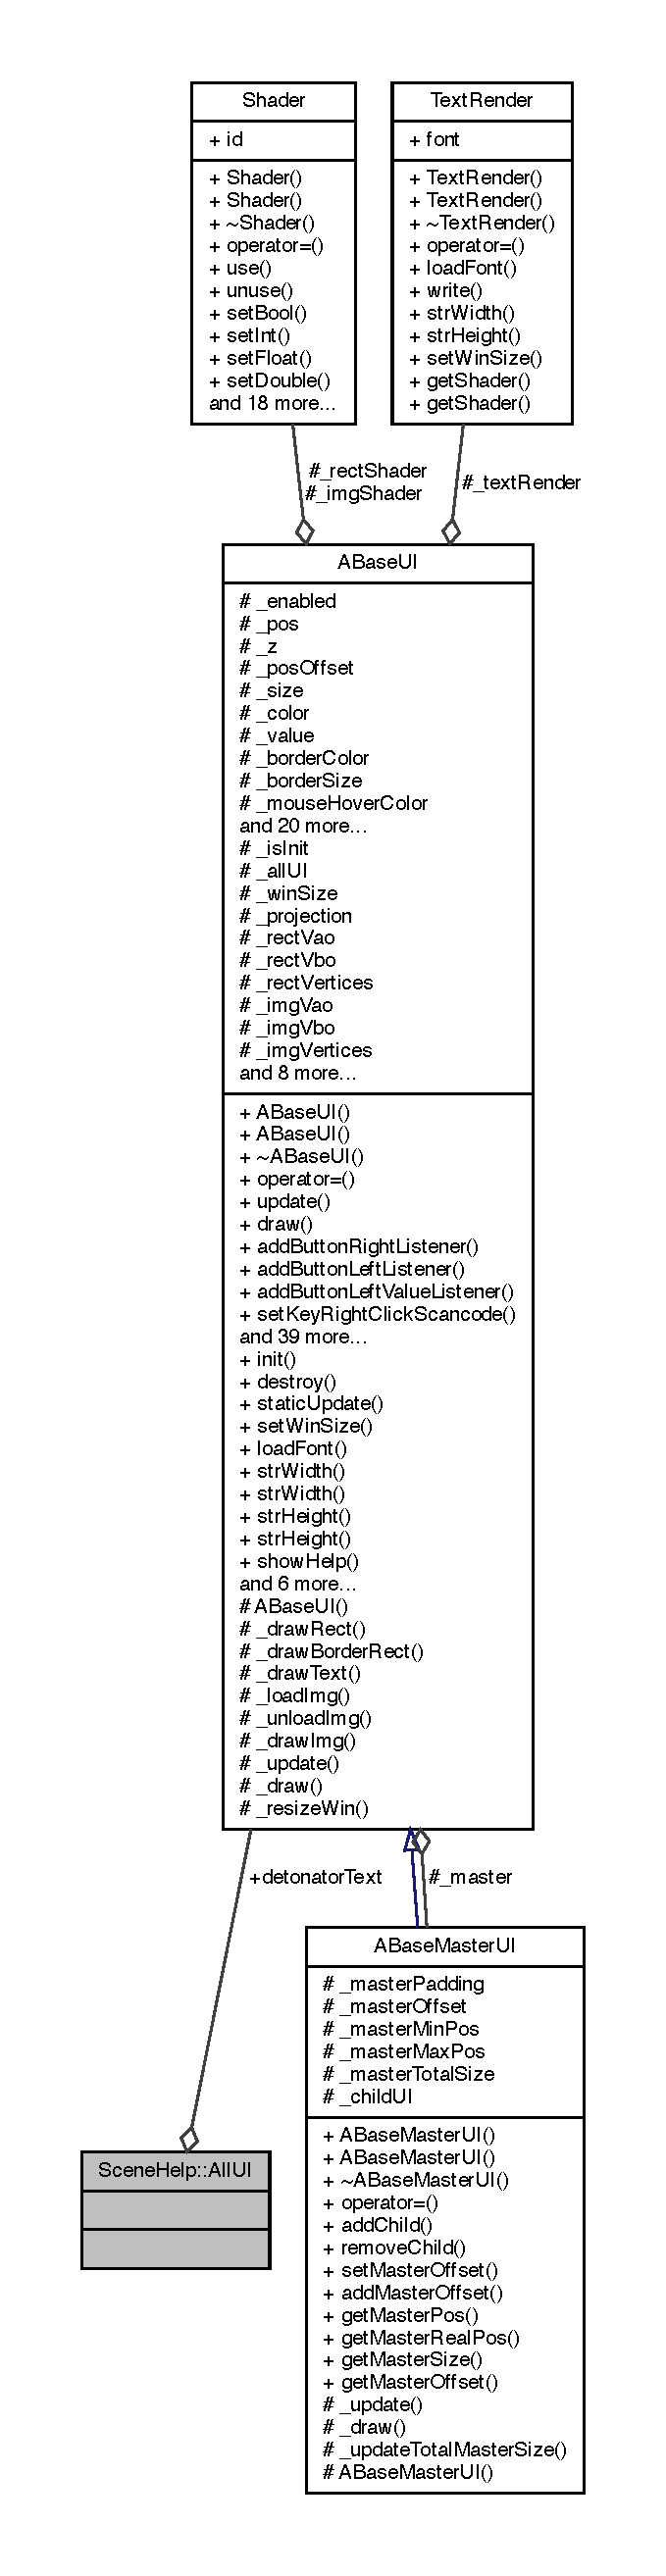
\includegraphics[height=550pt]{struct_scene_help_1_1_all_u_i__coll__graph}
\end{center}
\end{figure}
\doxysubsection*{Public Attributes}
\begin{DoxyCompactItemize}
\item 
\mbox{\hyperlink{class_a_base_u_i}{A\+Base\+UI}} $\ast$ \mbox{\hyperlink{struct_scene_help_1_1_all_u_i_ad96e5503ebdd34b0adc10a9eb6119ae7}{moving\+Text}}
\item 
\mbox{\hyperlink{class_a_base_u_i}{A\+Base\+UI}} $\ast$ \mbox{\hyperlink{struct_scene_help_1_1_all_u_i_ab0e1105d8d03dd6343b255d371a86446}{bomb\+Text}}
\item 
\mbox{\hyperlink{class_a_base_u_i}{A\+Base\+UI}} $\ast$ \mbox{\hyperlink{struct_scene_help_1_1_all_u_i_a8f7e4b57ab57eae00de7bb32186a8913}{bomb\+Detonator\+Text}}
\item 
\mbox{\hyperlink{class_a_base_u_i}{A\+Base\+UI}} $\ast$ \mbox{\hyperlink{struct_scene_help_1_1_all_u_i_ab4a49940220f4c2b057995265d227d89}{detonator\+Text}}
\item 
\mbox{\hyperlink{class_a_base_u_i}{A\+Base\+UI}} $\ast$ \mbox{\hyperlink{struct_scene_help_1_1_all_u_i_a06ae738b9d7798bb85bc9ed96f6e2561}{left\+Page}}
\item 
\mbox{\hyperlink{class_a_base_u_i}{A\+Base\+UI}} $\ast$ \mbox{\hyperlink{struct_scene_help_1_1_all_u_i_a0e3069e7a066ec6bed4c4f68f92c7ea0}{right\+Page}}
\item 
std\+::vector$<$ std\+::vector$<$ \mbox{\hyperlink{class_a_base_u_i}{A\+Base\+UI}} $\ast$ $>$ $>$ \mbox{\hyperlink{struct_scene_help_1_1_all_u_i_a6751dd1c672f9df65c99aa48e09ca713}{all\+Pages}}
\end{DoxyCompactItemize}


\doxysubsection{Detailed Description}
All UI elements. 

\doxysubsection{Member Data Documentation}
\mbox{\Hypertarget{struct_scene_help_1_1_all_u_i_a6751dd1c672f9df65c99aa48e09ca713}\label{struct_scene_help_1_1_all_u_i_a6751dd1c672f9df65c99aa48e09ca713}} 
\index{SceneHelp::AllUI@{SceneHelp::AllUI}!allPages@{allPages}}
\index{allPages@{allPages}!SceneHelp::AllUI@{SceneHelp::AllUI}}
\doxysubsubsection{\texorpdfstring{allPages}{allPages}}
{\footnotesize\ttfamily std\+::vector$<$ std\+::vector$<$ \mbox{\hyperlink{class_a_base_u_i}{A\+Base\+UI}}$\ast$ $>$ $>$ Scene\+Help\+::\+All\+U\+I\+::all\+Pages}

UI for all pages \mbox{\Hypertarget{struct_scene_help_1_1_all_u_i_a8f7e4b57ab57eae00de7bb32186a8913}\label{struct_scene_help_1_1_all_u_i_a8f7e4b57ab57eae00de7bb32186a8913}} 
\index{SceneHelp::AllUI@{SceneHelp::AllUI}!bombDetonatorText@{bombDetonatorText}}
\index{bombDetonatorText@{bombDetonatorText}!SceneHelp::AllUI@{SceneHelp::AllUI}}
\doxysubsubsection{\texorpdfstring{bombDetonatorText}{bombDetonatorText}}
{\footnotesize\ttfamily \mbox{\hyperlink{class_a_base_u_i}{A\+Base\+UI}}$\ast$ Scene\+Help\+::\+All\+U\+I\+::bomb\+Detonator\+Text}

UI for text in page 1 for detonator \mbox{\Hypertarget{struct_scene_help_1_1_all_u_i_ab0e1105d8d03dd6343b255d371a86446}\label{struct_scene_help_1_1_all_u_i_ab0e1105d8d03dd6343b255d371a86446}} 
\index{SceneHelp::AllUI@{SceneHelp::AllUI}!bombText@{bombText}}
\index{bombText@{bombText}!SceneHelp::AllUI@{SceneHelp::AllUI}}
\doxysubsubsection{\texorpdfstring{bombText}{bombText}}
{\footnotesize\ttfamily \mbox{\hyperlink{class_a_base_u_i}{A\+Base\+UI}}$\ast$ Scene\+Help\+::\+All\+U\+I\+::bomb\+Text}

UI for text in page 1 for bomb \mbox{\Hypertarget{struct_scene_help_1_1_all_u_i_ab4a49940220f4c2b057995265d227d89}\label{struct_scene_help_1_1_all_u_i_ab4a49940220f4c2b057995265d227d89}} 
\index{SceneHelp::AllUI@{SceneHelp::AllUI}!detonatorText@{detonatorText}}
\index{detonatorText@{detonatorText}!SceneHelp::AllUI@{SceneHelp::AllUI}}
\doxysubsubsection{\texorpdfstring{detonatorText}{detonatorText}}
{\footnotesize\ttfamily \mbox{\hyperlink{class_a_base_u_i}{A\+Base\+UI}}$\ast$ Scene\+Help\+::\+All\+U\+I\+::detonator\+Text}

UI for text in page 2 of detonator \mbox{\Hypertarget{struct_scene_help_1_1_all_u_i_a06ae738b9d7798bb85bc9ed96f6e2561}\label{struct_scene_help_1_1_all_u_i_a06ae738b9d7798bb85bc9ed96f6e2561}} 
\index{SceneHelp::AllUI@{SceneHelp::AllUI}!leftPage@{leftPage}}
\index{leftPage@{leftPage}!SceneHelp::AllUI@{SceneHelp::AllUI}}
\doxysubsubsection{\texorpdfstring{leftPage}{leftPage}}
{\footnotesize\ttfamily \mbox{\hyperlink{class_a_base_u_i}{A\+Base\+UI}}$\ast$ Scene\+Help\+::\+All\+U\+I\+::left\+Page}

UI for left page button \mbox{\Hypertarget{struct_scene_help_1_1_all_u_i_ad96e5503ebdd34b0adc10a9eb6119ae7}\label{struct_scene_help_1_1_all_u_i_ad96e5503ebdd34b0adc10a9eb6119ae7}} 
\index{SceneHelp::AllUI@{SceneHelp::AllUI}!movingText@{movingText}}
\index{movingText@{movingText}!SceneHelp::AllUI@{SceneHelp::AllUI}}
\doxysubsubsection{\texorpdfstring{movingText}{movingText}}
{\footnotesize\ttfamily \mbox{\hyperlink{class_a_base_u_i}{A\+Base\+UI}}$\ast$ Scene\+Help\+::\+All\+U\+I\+::moving\+Text}

UI for text in page 1 for moving \mbox{\Hypertarget{struct_scene_help_1_1_all_u_i_a0e3069e7a066ec6bed4c4f68f92c7ea0}\label{struct_scene_help_1_1_all_u_i_a0e3069e7a066ec6bed4c4f68f92c7ea0}} 
\index{SceneHelp::AllUI@{SceneHelp::AllUI}!rightPage@{rightPage}}
\index{rightPage@{rightPage}!SceneHelp::AllUI@{SceneHelp::AllUI}}
\doxysubsubsection{\texorpdfstring{rightPage}{rightPage}}
{\footnotesize\ttfamily \mbox{\hyperlink{class_a_base_u_i}{A\+Base\+UI}}$\ast$ Scene\+Help\+::\+All\+U\+I\+::right\+Page}

UI for right page button 

The documentation for this struct was generated from the following file\+:\begin{DoxyCompactItemize}
\item 
includes/scenes/Scene\+Help.\+hpp\end{DoxyCompactItemize}

\hypertarget{struct_scene_level_selection_1_1_all_u_i}{}\doxysection{Scene\+Level\+Selection\+::All\+UI Struct Reference}
\label{struct_scene_level_selection_1_1_all_u_i}\index{SceneLevelSelection::AllUI@{SceneLevelSelection::AllUI}}


Collaboration diagram for Scene\+Level\+Selection\+::All\+UI\+:
\nopagebreak
\begin{figure}[H]
\begin{center}
\leavevmode
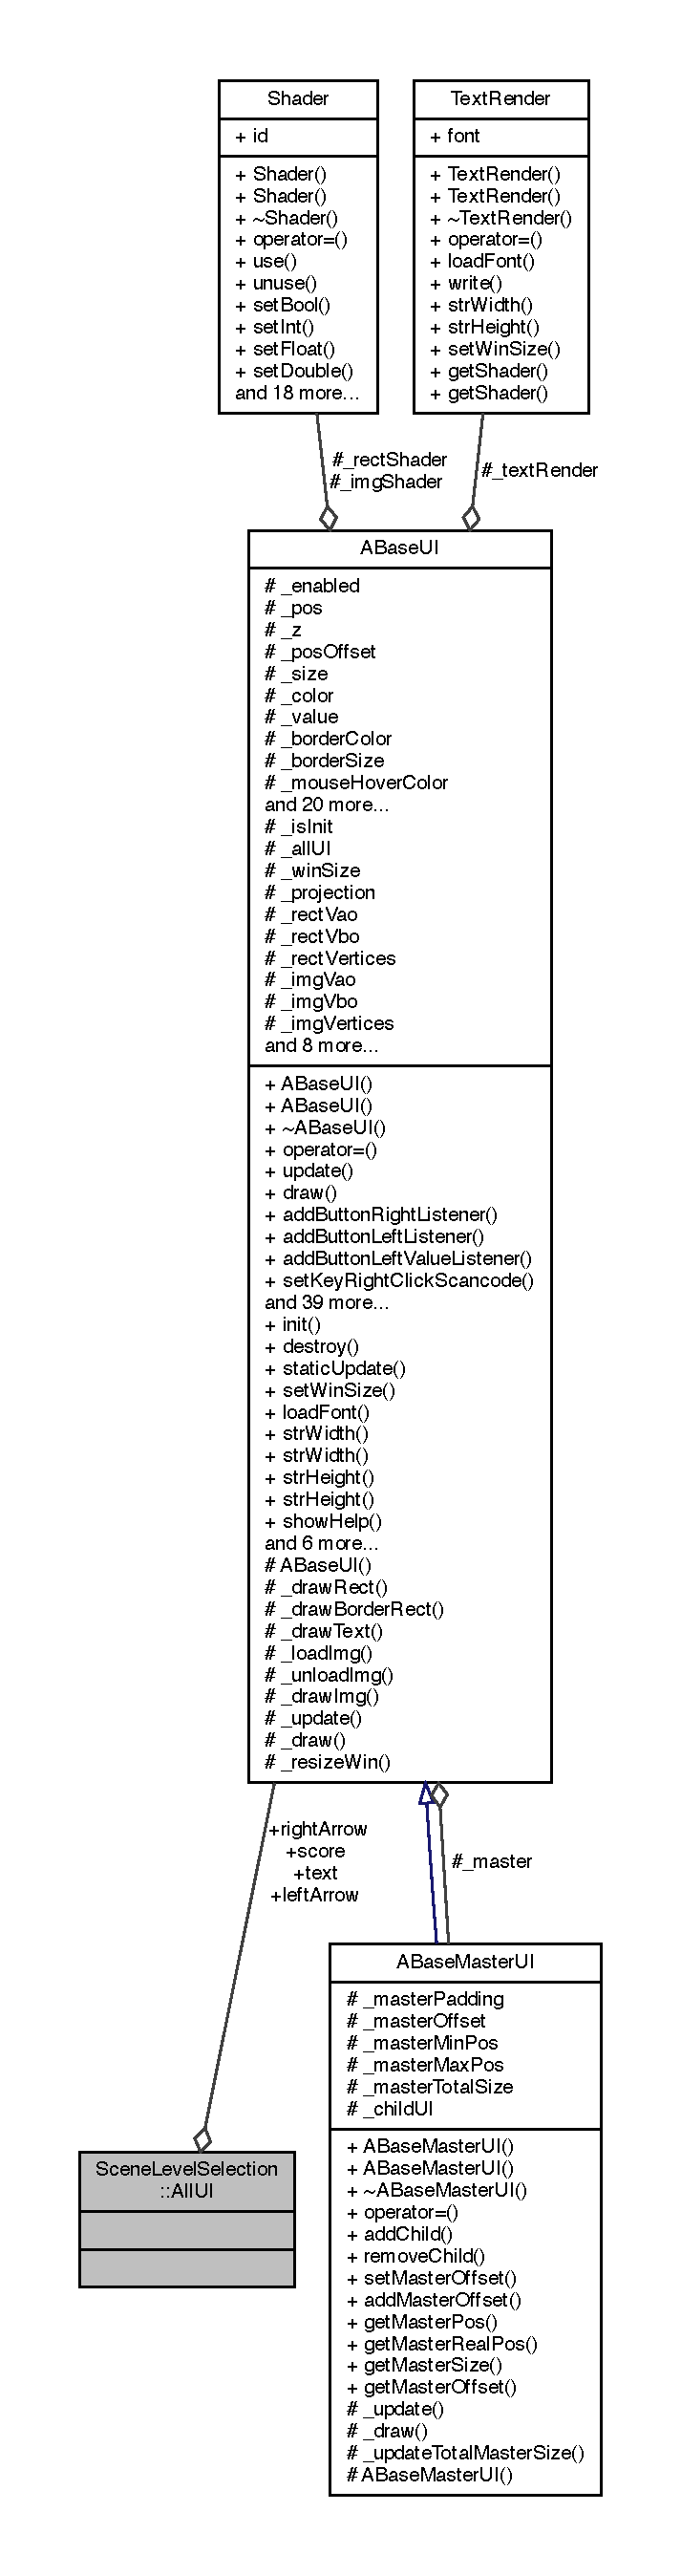
\includegraphics[height=550pt]{struct_scene_level_selection_1_1_all_u_i__coll__graph}
\end{center}
\end{figure}
\doxysubsection*{Public Attributes}
\begin{DoxyCompactItemize}
\item 
\mbox{\Hypertarget{struct_scene_level_selection_1_1_all_u_i_ad2d0b933a964466a4a007a485f8e08aa}\label{struct_scene_level_selection_1_1_all_u_i_ad2d0b933a964466a4a007a485f8e08aa}} 
\mbox{\hyperlink{class_a_base_u_i}{A\+Base\+UI}} $\ast$ {\bfseries text}
\item 
\mbox{\Hypertarget{struct_scene_level_selection_1_1_all_u_i_a56609f362dab95f3b13aa649e1c86004}\label{struct_scene_level_selection_1_1_all_u_i_a56609f362dab95f3b13aa649e1c86004}} 
\mbox{\hyperlink{class_a_base_u_i}{A\+Base\+UI}} $\ast$ {\bfseries score}
\item 
\mbox{\Hypertarget{struct_scene_level_selection_1_1_all_u_i_a9368995814a5c08871309e9a38765a6e}\label{struct_scene_level_selection_1_1_all_u_i_a9368995814a5c08871309e9a38765a6e}} 
\mbox{\hyperlink{class_a_base_u_i}{A\+Base\+UI}} $\ast$ {\bfseries left\+Arrow}
\item 
\mbox{\Hypertarget{struct_scene_level_selection_1_1_all_u_i_abdef1035e3e42b604196d33ae6b4e04a}\label{struct_scene_level_selection_1_1_all_u_i_abdef1035e3e42b604196d33ae6b4e04a}} 
\mbox{\hyperlink{class_a_base_u_i}{A\+Base\+UI}} $\ast$ {\bfseries right\+Arrow}
\end{DoxyCompactItemize}


The documentation for this struct was generated from the following file\+:\begin{DoxyCompactItemize}
\item 
includes/scenes/Scene\+Level\+Selection.\+hpp\end{DoxyCompactItemize}

\hypertarget{struct_scene_main_menu_1_1_all_u_i}{}\doxysection{Scene\+Main\+Menu\+::All\+UI Struct Reference}
\label{struct_scene_main_menu_1_1_all_u_i}\index{SceneMainMenu::AllUI@{SceneMainMenu::AllUI}}


Collaboration diagram for Scene\+Main\+Menu\+::All\+UI\+:\nopagebreak
\begin{figure}[H]
\begin{center}
\leavevmode
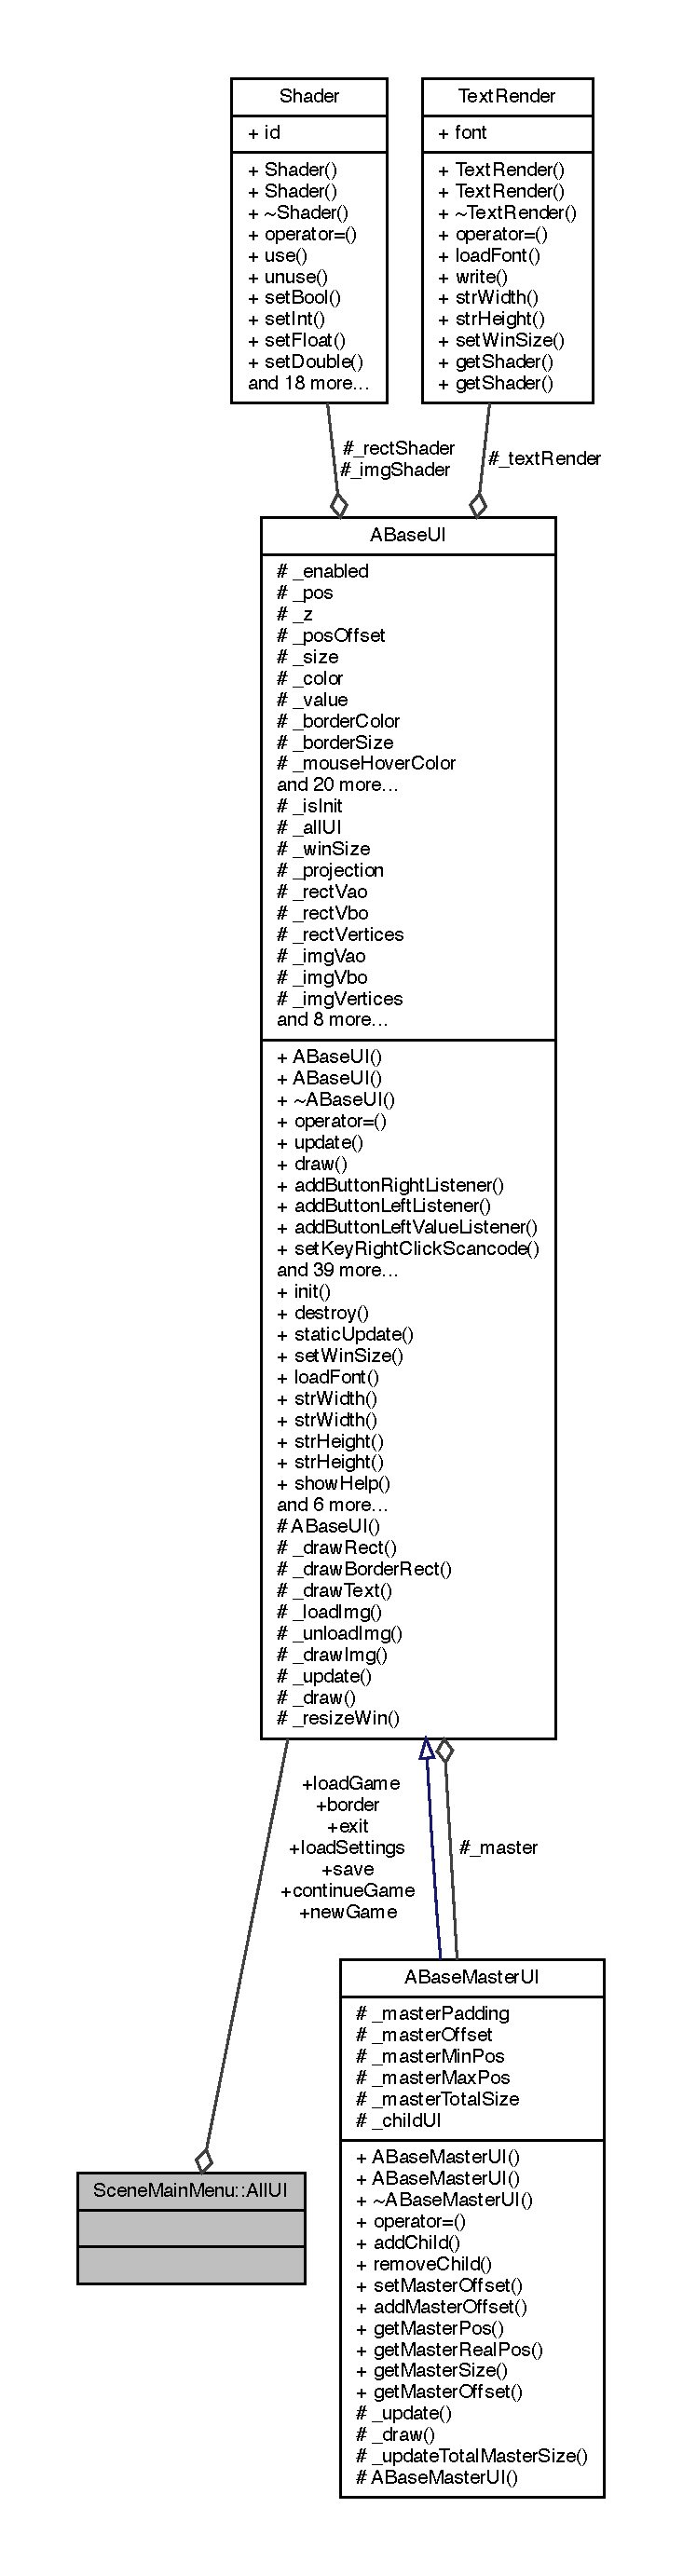
\includegraphics[height=550pt]{struct_scene_main_menu_1_1_all_u_i__coll__graph}
\end{center}
\end{figure}
\doxysubsection*{Public Attributes}
\begin{DoxyCompactItemize}
\item 
\mbox{\Hypertarget{struct_scene_main_menu_1_1_all_u_i_acbfc7a90c7fe59b0f5c452f37944238d}\label{struct_scene_main_menu_1_1_all_u_i_acbfc7a90c7fe59b0f5c452f37944238d}} 
\mbox{\hyperlink{class_a_base_u_i}{A\+Base\+UI}} $\ast$ {\bfseries continue\+Game}
\item 
\mbox{\Hypertarget{struct_scene_main_menu_1_1_all_u_i_a801aade41279dd9c41b1c09b1ab74459}\label{struct_scene_main_menu_1_1_all_u_i_a801aade41279dd9c41b1c09b1ab74459}} 
\mbox{\hyperlink{class_a_base_u_i}{A\+Base\+UI}} $\ast$ {\bfseries save}
\item 
\mbox{\Hypertarget{struct_scene_main_menu_1_1_all_u_i_a51cbd15371ce654749adf34402e64aed}\label{struct_scene_main_menu_1_1_all_u_i_a51cbd15371ce654749adf34402e64aed}} 
\mbox{\hyperlink{class_a_base_u_i}{A\+Base\+UI}} $\ast$ {\bfseries new\+Game}
\item 
\mbox{\Hypertarget{struct_scene_main_menu_1_1_all_u_i_af40f78e33f1a3674fab5c83ce44338f3}\label{struct_scene_main_menu_1_1_all_u_i_af40f78e33f1a3674fab5c83ce44338f3}} 
\mbox{\hyperlink{class_a_base_u_i}{A\+Base\+UI}} $\ast$ {\bfseries load\+Game}
\item 
\mbox{\Hypertarget{struct_scene_main_menu_1_1_all_u_i_ab29e5beed68a4762fb48ccc01989c6bb}\label{struct_scene_main_menu_1_1_all_u_i_ab29e5beed68a4762fb48ccc01989c6bb}} 
\mbox{\hyperlink{class_a_base_u_i}{A\+Base\+UI}} $\ast$ {\bfseries load\+Settings}
\item 
\mbox{\Hypertarget{struct_scene_main_menu_1_1_all_u_i_ab8266966efdf73dac22cf85f67a1f9de}\label{struct_scene_main_menu_1_1_all_u_i_ab8266966efdf73dac22cf85f67a1f9de}} 
\mbox{\hyperlink{class_a_base_u_i}{A\+Base\+UI}} $\ast$ {\bfseries exit}
\item 
\mbox{\Hypertarget{struct_scene_main_menu_1_1_all_u_i_ae0a3df76b19cfbde641c126be24c327a}\label{struct_scene_main_menu_1_1_all_u_i_ae0a3df76b19cfbde641c126be24c327a}} 
\mbox{\hyperlink{class_a_base_u_i}{A\+Base\+UI}} $\ast$ {\bfseries border}
\end{DoxyCompactItemize}


The documentation for this struct was generated from the following file\+:\begin{DoxyCompactItemize}
\item 
includes/scenes/Scene\+Main\+Menu.\+hpp\end{DoxyCompactItemize}

\hypertarget{struct_scene_difficulty_1_1_all_u_i}{}\doxysection{Scene\+Difficulty\+::All\+UI Struct Reference}
\label{struct_scene_difficulty_1_1_all_u_i}\index{SceneDifficulty::AllUI@{SceneDifficulty::AllUI}}


All UI elements.  




{\ttfamily \#include $<$Scene\+Difficulty.\+hpp$>$}



Collaboration diagram for Scene\+Difficulty\+::All\+UI\+:\nopagebreak
\begin{figure}[H]
\begin{center}
\leavevmode
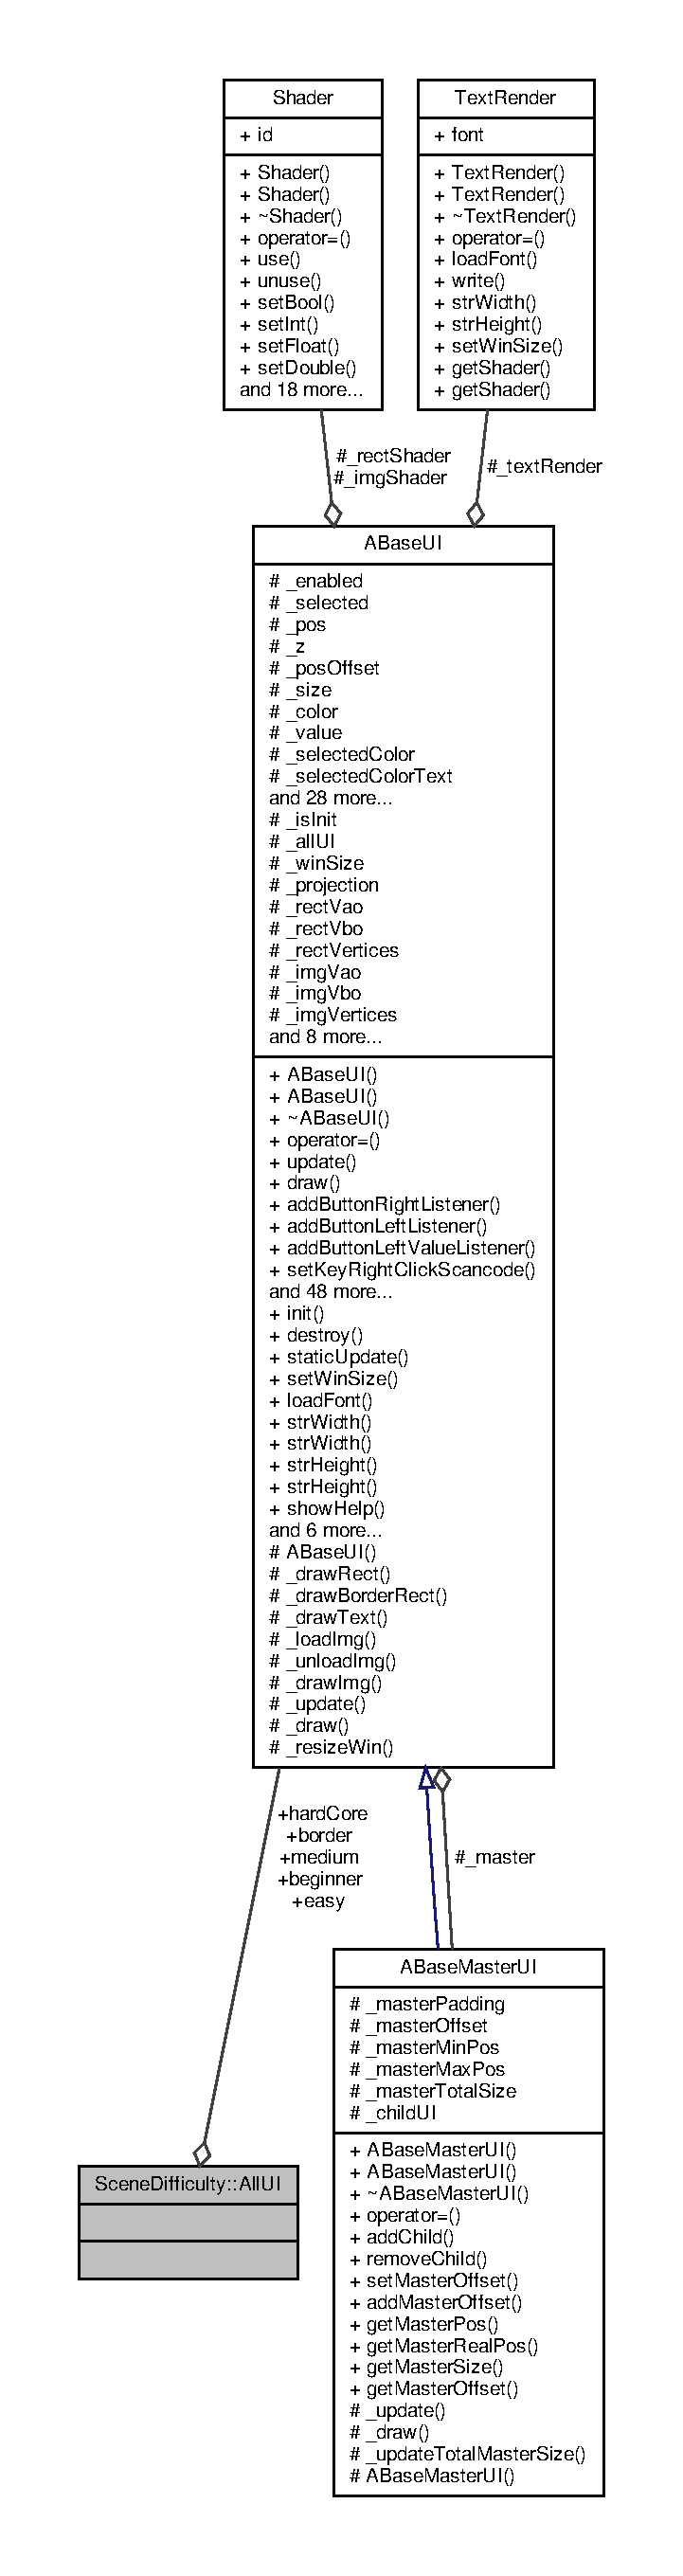
\includegraphics[height=550pt]{struct_scene_difficulty_1_1_all_u_i__coll__graph}
\end{center}
\end{figure}
\doxysubsection*{Public Attributes}
\begin{DoxyCompactItemize}
\item 
\mbox{\hyperlink{class_a_base_u_i}{A\+Base\+UI}} $\ast$ \mbox{\hyperlink{struct_scene_difficulty_1_1_all_u_i_a7b47580f2e606f79f2d117c7d348aad7}{beginner}}
\item 
\mbox{\hyperlink{class_a_base_u_i}{A\+Base\+UI}} $\ast$ \mbox{\hyperlink{struct_scene_difficulty_1_1_all_u_i_acb9d7c8cb4617cfc353f475bec54b19e}{easy}}
\item 
\mbox{\hyperlink{class_a_base_u_i}{A\+Base\+UI}} $\ast$ \mbox{\hyperlink{struct_scene_difficulty_1_1_all_u_i_a19bd705042ffd4a8d8bddf7aa4959ae4}{medium}}
\item 
\mbox{\hyperlink{class_a_base_u_i}{A\+Base\+UI}} $\ast$ \mbox{\hyperlink{struct_scene_difficulty_1_1_all_u_i_a0d3c51dfb0a9635f2bc4d76fe707b3a3}{hard\+Core}}
\item 
\mbox{\hyperlink{class_a_base_u_i}{A\+Base\+UI}} $\ast$ \mbox{\hyperlink{struct_scene_difficulty_1_1_all_u_i_a8c0a119bef1acfe64138fd5b9fc9442d}{border}}
\end{DoxyCompactItemize}


\doxysubsection{Detailed Description}
All UI elements. 

\doxysubsection{Member Data Documentation}
\mbox{\Hypertarget{struct_scene_difficulty_1_1_all_u_i_a7b47580f2e606f79f2d117c7d348aad7}\label{struct_scene_difficulty_1_1_all_u_i_a7b47580f2e606f79f2d117c7d348aad7}} 
\index{SceneDifficulty::AllUI@{SceneDifficulty::AllUI}!beginner@{beginner}}
\index{beginner@{beginner}!SceneDifficulty::AllUI@{SceneDifficulty::AllUI}}
\doxysubsubsection{\texorpdfstring{beginner}{beginner}}
{\footnotesize\ttfamily \mbox{\hyperlink{class_a_base_u_i}{A\+Base\+UI}}$\ast$ Scene\+Difficulty\+::\+All\+U\+I\+::beginner}

UI for beginner element \mbox{\Hypertarget{struct_scene_difficulty_1_1_all_u_i_a8c0a119bef1acfe64138fd5b9fc9442d}\label{struct_scene_difficulty_1_1_all_u_i_a8c0a119bef1acfe64138fd5b9fc9442d}} 
\index{SceneDifficulty::AllUI@{SceneDifficulty::AllUI}!border@{border}}
\index{border@{border}!SceneDifficulty::AllUI@{SceneDifficulty::AllUI}}
\doxysubsubsection{\texorpdfstring{border}{border}}
{\footnotesize\ttfamily \mbox{\hyperlink{class_a_base_u_i}{A\+Base\+UI}}$\ast$ Scene\+Difficulty\+::\+All\+U\+I\+::border}

UI for border element \mbox{\Hypertarget{struct_scene_difficulty_1_1_all_u_i_acb9d7c8cb4617cfc353f475bec54b19e}\label{struct_scene_difficulty_1_1_all_u_i_acb9d7c8cb4617cfc353f475bec54b19e}} 
\index{SceneDifficulty::AllUI@{SceneDifficulty::AllUI}!easy@{easy}}
\index{easy@{easy}!SceneDifficulty::AllUI@{SceneDifficulty::AllUI}}
\doxysubsubsection{\texorpdfstring{easy}{easy}}
{\footnotesize\ttfamily \mbox{\hyperlink{class_a_base_u_i}{A\+Base\+UI}}$\ast$ Scene\+Difficulty\+::\+All\+U\+I\+::easy}

UI for easy element \mbox{\Hypertarget{struct_scene_difficulty_1_1_all_u_i_a0d3c51dfb0a9635f2bc4d76fe707b3a3}\label{struct_scene_difficulty_1_1_all_u_i_a0d3c51dfb0a9635f2bc4d76fe707b3a3}} 
\index{SceneDifficulty::AllUI@{SceneDifficulty::AllUI}!hardCore@{hardCore}}
\index{hardCore@{hardCore}!SceneDifficulty::AllUI@{SceneDifficulty::AllUI}}
\doxysubsubsection{\texorpdfstring{hardCore}{hardCore}}
{\footnotesize\ttfamily \mbox{\hyperlink{class_a_base_u_i}{A\+Base\+UI}}$\ast$ Scene\+Difficulty\+::\+All\+U\+I\+::hard\+Core}

UI for hard\+Core element \mbox{\Hypertarget{struct_scene_difficulty_1_1_all_u_i_a19bd705042ffd4a8d8bddf7aa4959ae4}\label{struct_scene_difficulty_1_1_all_u_i_a19bd705042ffd4a8d8bddf7aa4959ae4}} 
\index{SceneDifficulty::AllUI@{SceneDifficulty::AllUI}!medium@{medium}}
\index{medium@{medium}!SceneDifficulty::AllUI@{SceneDifficulty::AllUI}}
\doxysubsubsection{\texorpdfstring{medium}{medium}}
{\footnotesize\ttfamily \mbox{\hyperlink{class_a_base_u_i}{A\+Base\+UI}}$\ast$ Scene\+Difficulty\+::\+All\+U\+I\+::medium}

UI for medium element 

The documentation for this struct was generated from the following file\+:\begin{DoxyCompactItemize}
\item 
includes/scenes/Scene\+Difficulty.\+hpp\end{DoxyCompactItemize}

\hypertarget{class_a_object}{}\doxysection{A\+Object Class Reference}
\label{class_a_object}\index{AObject@{AObject}}


This is the base class for objects (\mbox{\hyperlink{class_bomb}{Bomb}}, wall, ...)  




{\ttfamily \#include $<$A\+Object.\+hpp$>$}



Inheritance diagram for A\+Object\+:
\nopagebreak
\begin{figure}[H]
\begin{center}
\leavevmode
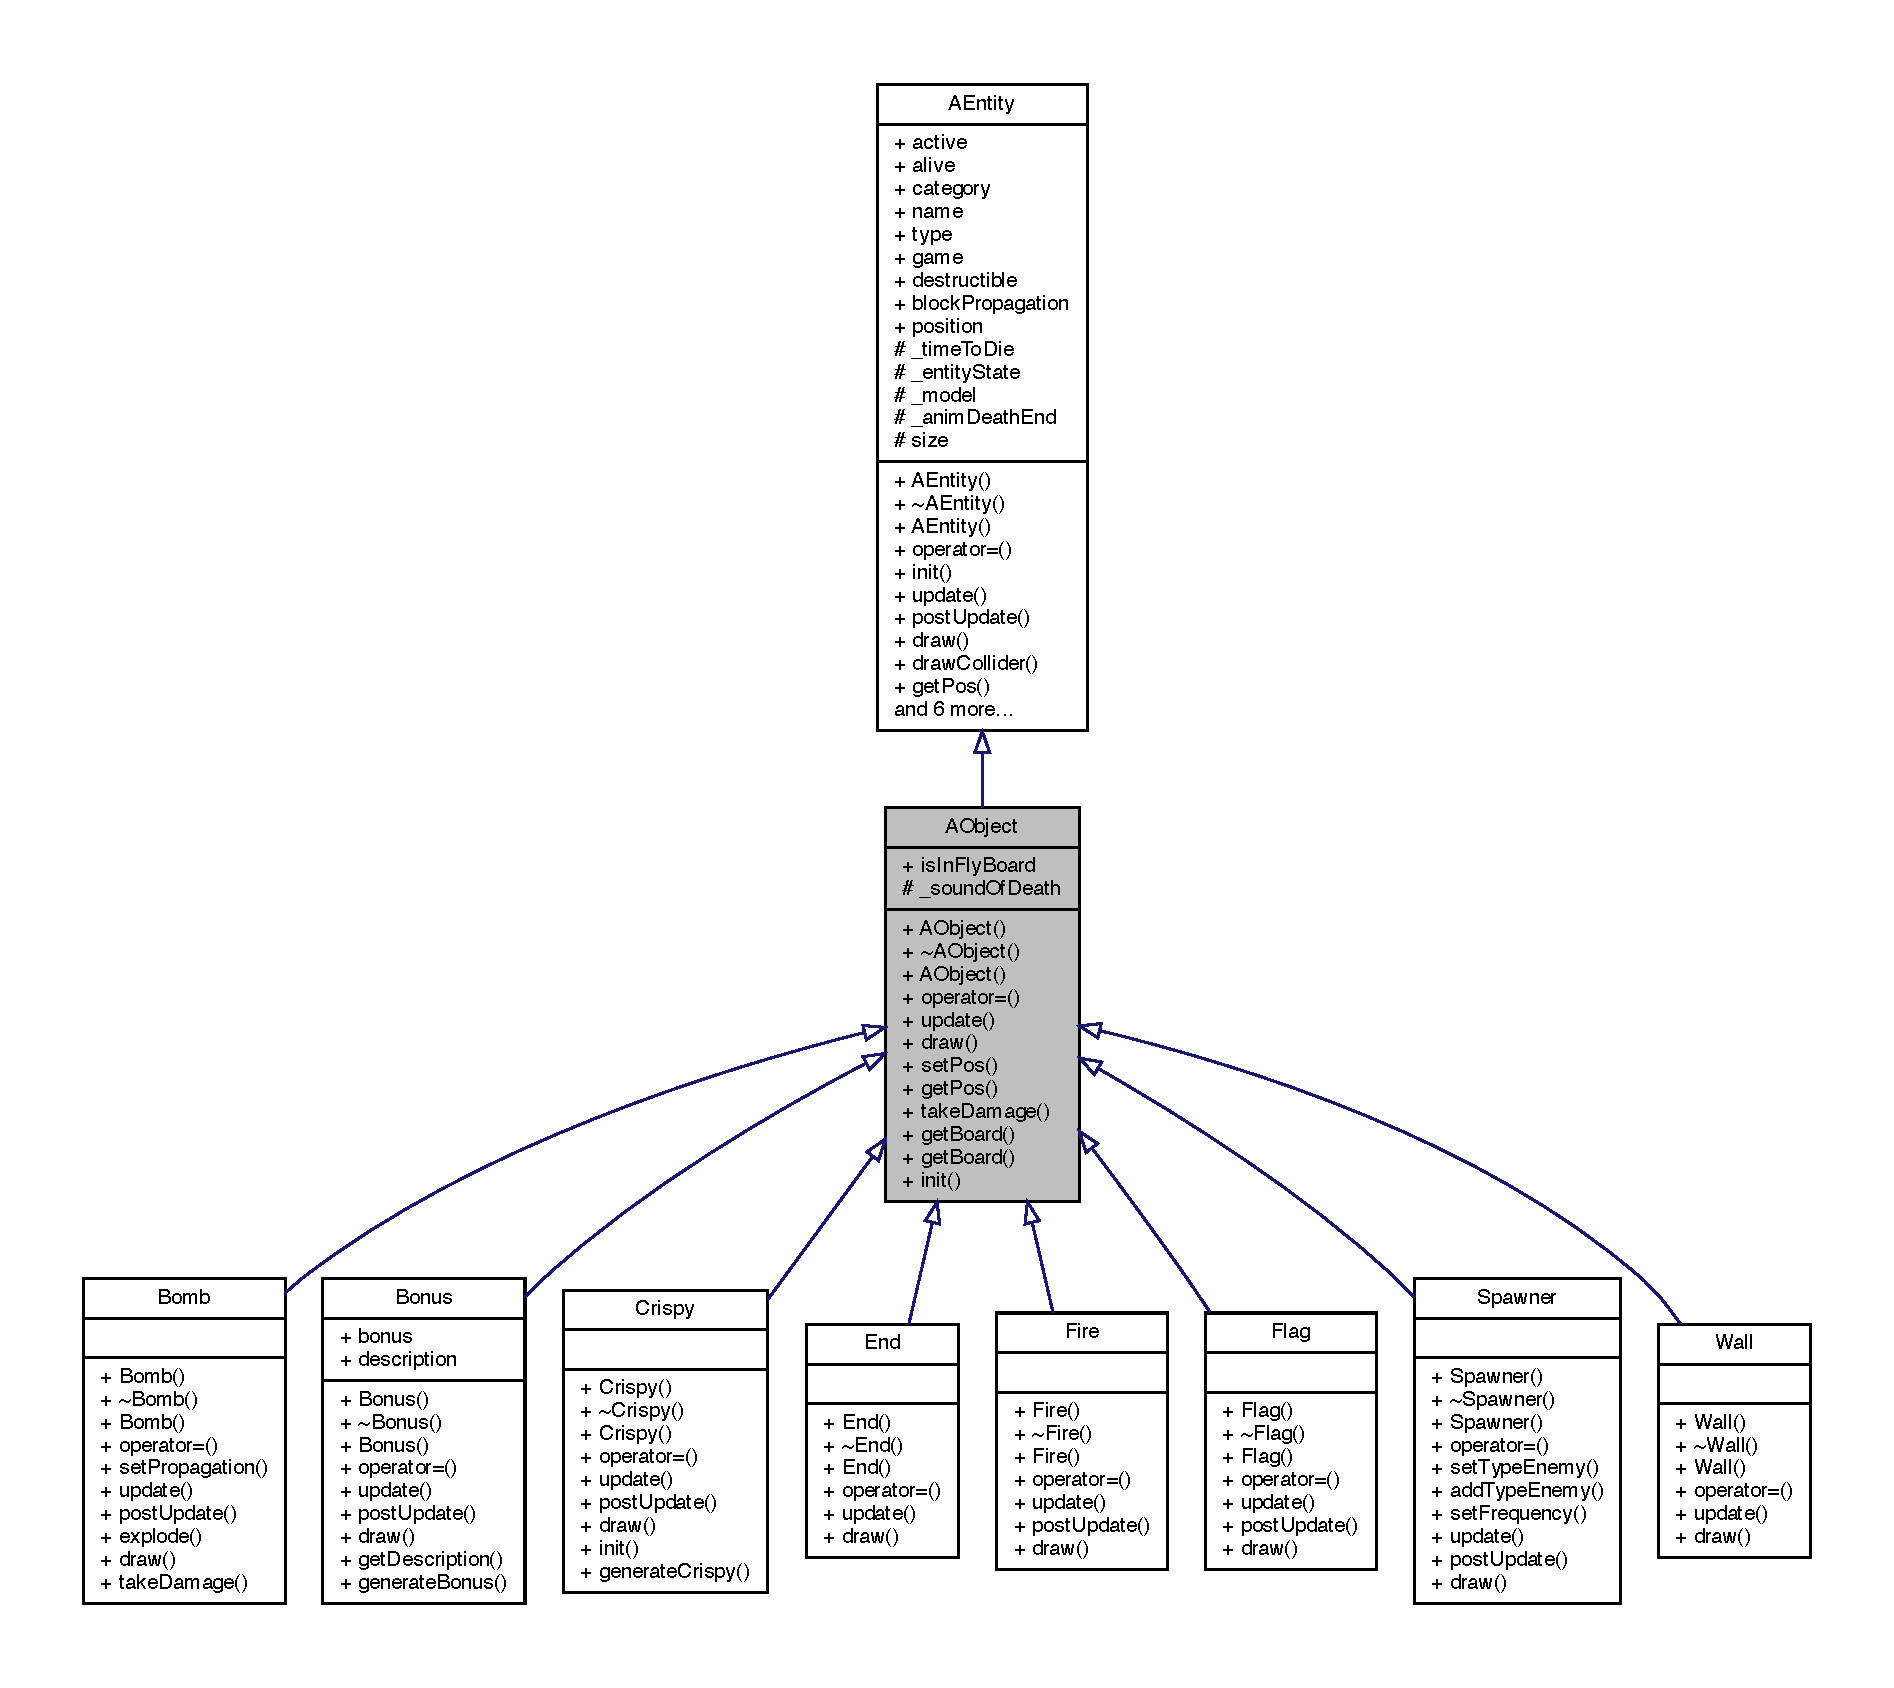
\includegraphics[width=350pt]{class_a_object__inherit__graph}
\end{center}
\end{figure}


Collaboration diagram for A\+Object\+:
\nopagebreak
\begin{figure}[H]
\begin{center}
\leavevmode
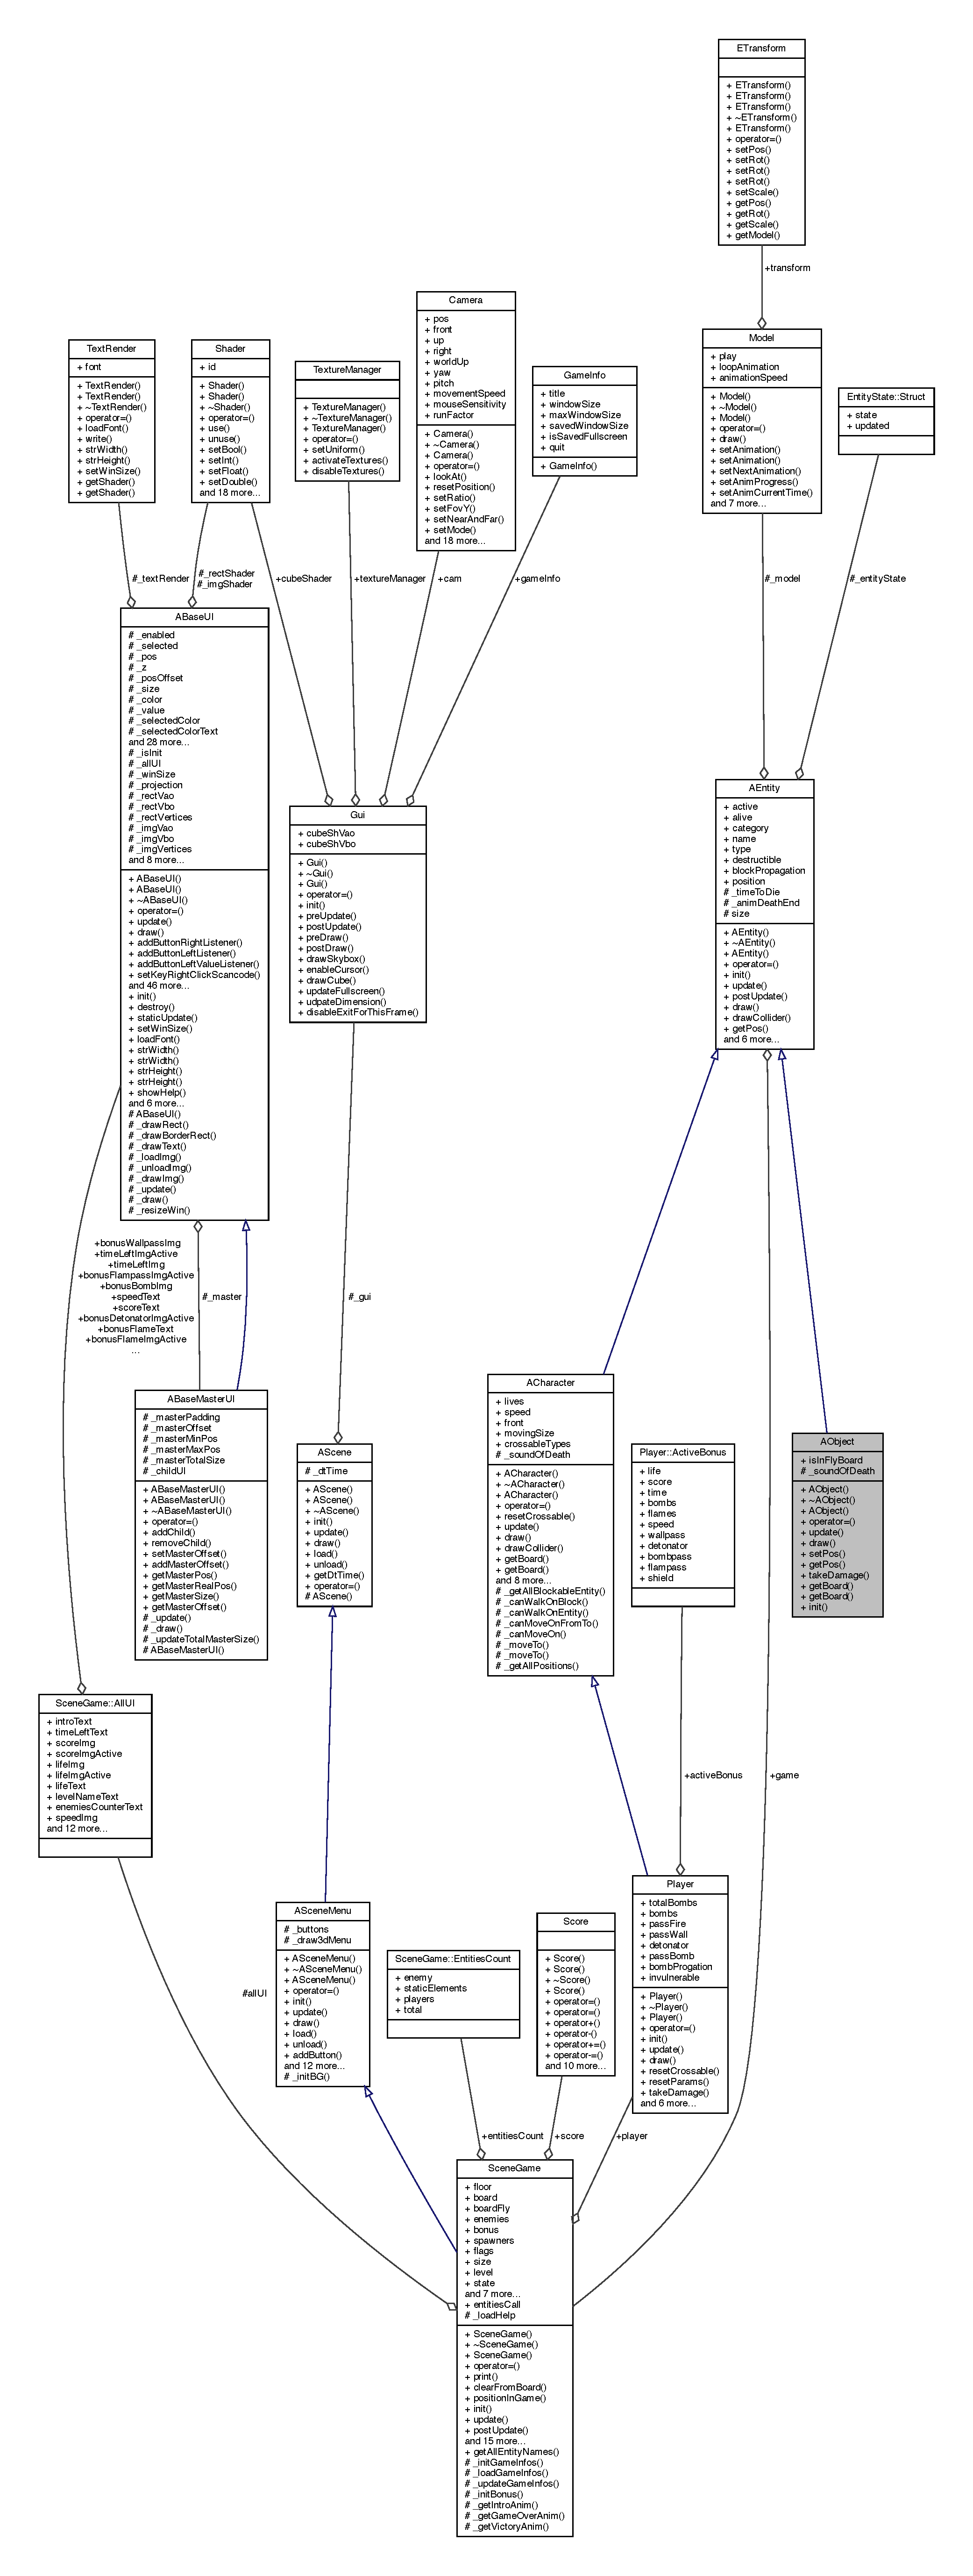
\includegraphics[height=550pt]{class_a_object__coll__graph}
\end{center}
\end{figure}
\doxysubsection*{Classes}
\begin{DoxyCompactItemize}
\item 
class \mbox{\hyperlink{class_a_object_1_1_a_object_exception}{A\+Object\+Exception}}
\begin{DoxyCompactList}\small\item\em \mbox{\hyperlink{class_a_object}{A\+Object}} Exception. \end{DoxyCompactList}\end{DoxyCompactItemize}
\doxysubsection*{Public Member Functions}
\begin{DoxyCompactItemize}
\item 
\mbox{\hyperlink{class_a_object_aac94ec1c7dd0ec00fda2a79f12195cf2}{A\+Object}} (\mbox{\hyperlink{class_scene_game}{Scene\+Game}} \&\mbox{\hyperlink{class_a_entity_aa2c05db944a8b7487eb8470dd20211ab}{game}})
\begin{DoxyCompactList}\small\item\em Construct a new A\+Object\+::\+A\+Object object. \end{DoxyCompactList}\item 
\mbox{\Hypertarget{class_a_object_ac17f3a1944792c280a3cbd83d839bc4e}\label{class_a_object_ac17f3a1944792c280a3cbd83d839bc4e}} 
virtual \mbox{\hyperlink{class_a_object_ac17f3a1944792c280a3cbd83d839bc4e}{$\sim$\+A\+Object}} ()
\begin{DoxyCompactList}\small\item\em Destroy the A\+Object\+::\+A\+Object object. \end{DoxyCompactList}\item 
\mbox{\hyperlink{class_a_object_a278727c68ad694b228c2f24e5e6d358a}{A\+Object}} (\mbox{\hyperlink{class_a_object}{A\+Object}} const \&src)
\begin{DoxyCompactList}\small\item\em Construct a new A\+Object\+::\+A\+Object object. \end{DoxyCompactList}\item 
\mbox{\hyperlink{class_a_object}{A\+Object}} \& \mbox{\hyperlink{class_a_object_a9752ad3eadac3a51ef78d81a34fc5bcd}{operator=}} (\mbox{\hyperlink{class_a_object}{A\+Object}} const \&rhs)
\begin{DoxyCompactList}\small\item\em Overloaded operator. \end{DoxyCompactList}\item 
virtual bool \mbox{\hyperlink{class_a_object_af35bb4b68af0a11bb1fcf617bde41ecd}{update}} ()=0
\begin{DoxyCompactList}\small\item\em Update object. Called on every frames. \end{DoxyCompactList}\item 
virtual bool \mbox{\hyperlink{class_a_object_a5e454e13e04ee937c20a465244cf748a}{draw}} (\mbox{\hyperlink{class_gui}{Gui}} \&gui)=0
\begin{DoxyCompactList}\small\item\em Draw object. Called on every frames. \end{DoxyCompactList}\item 
void \mbox{\hyperlink{class_a_object_ac254ff8c08640e01dd5fbe030b4d89bc}{set\+Pos}} (glm\+::vec3 pos=V\+O\+I\+D\+\_\+\+P\+O\+S3)
\begin{DoxyCompactList}\small\item\em Set the position of the object according of his position on the board. \end{DoxyCompactList}\item 
glm\+::vec3 \mbox{\hyperlink{class_a_object_ab5840de6100bba8bf93a186a0a802708}{get\+Pos}} () const
\begin{DoxyCompactList}\small\item\em Get the position of the current \mbox{\hyperlink{class_a_object}{A\+Object}} in the \mbox{\hyperlink{class_scene_game_a2306af8a268c9d476d1060fa3daa1ac5}{Scene\+Game\+::board}} of this-\/$>$game. \end{DoxyCompactList}\item 
bool \mbox{\hyperlink{class_a_object_a39b1720ae5a820512ab4db0906f03b15}{take\+Damage}} (int damage)
\begin{DoxyCompactList}\small\item\em Take\+Damage put an object to die. \end{DoxyCompactList}\item 
virtual std\+::vector$<$ std\+::vector$<$ std\+::vector$<$ \mbox{\hyperlink{class_a_entity}{A\+Entity}} $\ast$ $>$ $>$ $>$ const  \& \mbox{\hyperlink{class_a_object_ac4a82eef484c0f7bf3547a7f7f6dce7e}{get\+Board}} () const
\begin{DoxyCompactList}\small\item\em Get the board (game.\+board or game.\+board\+Fly) \end{DoxyCompactList}\item 
virtual std\+::vector$<$ std\+::vector$<$ std\+::vector$<$ \mbox{\hyperlink{class_a_entity}{A\+Entity}} $\ast$ $>$ $>$ $>$ \& \mbox{\hyperlink{class_a_object_aba4b07c0456b2c3d42a71529ef40f2d5}{get\+Board}} ()
\begin{DoxyCompactList}\small\item\em Get the board (game.\+board or game.\+board\+Fly) \end{DoxyCompactList}\item 
virtual bool \mbox{\hyperlink{class_a_object_afa83ef1c900a47453524219788327b86}{init}} ()
\begin{DoxyCompactList}\small\item\em Init \mbox{\hyperlink{class_a_object}{A\+Object}}. \end{DoxyCompactList}\end{DoxyCompactItemize}
\doxysubsection*{Public Attributes}
\begin{DoxyCompactItemize}
\item 
bool \mbox{\hyperlink{class_a_object_a32efabd4a159239aaebc75c15e542a35}{is\+In\+Fly\+Board}}
\end{DoxyCompactItemize}
\doxysubsection*{Protected Attributes}
\begin{DoxyCompactItemize}
\item 
std\+::string \mbox{\hyperlink{class_a_object_abd487a37ad66b909b7d082c9655d43e0}{\+\_\+sound\+Of\+Death}}
\end{DoxyCompactItemize}


\doxysubsection{Detailed Description}
This is the base class for objects (\mbox{\hyperlink{class_bomb}{Bomb}}, wall, ...) 

\doxysubsection{Constructor \& Destructor Documentation}
\mbox{\Hypertarget{class_a_object_aac94ec1c7dd0ec00fda2a79f12195cf2}\label{class_a_object_aac94ec1c7dd0ec00fda2a79f12195cf2}} 
\index{AObject@{AObject}!AObject@{AObject}}
\index{AObject@{AObject}!AObject@{AObject}}
\doxysubsubsection{\texorpdfstring{AObject()}{AObject()}\hspace{0.1cm}{\footnotesize\ttfamily [1/2]}}
{\footnotesize\ttfamily A\+Object\+::\+A\+Object (\begin{DoxyParamCaption}\item[{\mbox{\hyperlink{class_scene_game}{Scene\+Game}} \&}]{game }\end{DoxyParamCaption})\hspace{0.3cm}{\ttfamily [explicit]}}



Construct a new A\+Object\+::\+A\+Object object. 


\begin{DoxyParams}{Parameters}
{\em game} & A reference to the \mbox{\hyperlink{class_scene_game}{Scene\+Game}} object \\
\hline
\end{DoxyParams}
\mbox{\Hypertarget{class_a_object_a278727c68ad694b228c2f24e5e6d358a}\label{class_a_object_a278727c68ad694b228c2f24e5e6d358a}} 
\index{AObject@{AObject}!AObject@{AObject}}
\index{AObject@{AObject}!AObject@{AObject}}
\doxysubsubsection{\texorpdfstring{AObject()}{AObject()}\hspace{0.1cm}{\footnotesize\ttfamily [2/2]}}
{\footnotesize\ttfamily A\+Object\+::\+A\+Object (\begin{DoxyParamCaption}\item[{\mbox{\hyperlink{class_a_object}{A\+Object}} const \&}]{src }\end{DoxyParamCaption})}



Construct a new A\+Object\+::\+A\+Object object. 


\begin{DoxyParams}{Parameters}
{\em src} & A \mbox{\hyperlink{class_a_object}{A\+Object}} element to copy \\
\hline
\end{DoxyParams}


\doxysubsection{Member Function Documentation}
\mbox{\Hypertarget{class_a_object_a5e454e13e04ee937c20a465244cf748a}\label{class_a_object_a5e454e13e04ee937c20a465244cf748a}} 
\index{AObject@{AObject}!draw@{draw}}
\index{draw@{draw}!AObject@{AObject}}
\doxysubsubsection{\texorpdfstring{draw()}{draw()}}
{\footnotesize\ttfamily virtual bool A\+Object\+::draw (\begin{DoxyParamCaption}\item[{\mbox{\hyperlink{class_gui}{Gui}} \&}]{gui }\end{DoxyParamCaption})\hspace{0.3cm}{\ttfamily [pure virtual]}}



Draw object. Called on every frames. 

\begin{DoxyReturn}{Returns}
false If failed 
\end{DoxyReturn}


Implements \mbox{\hyperlink{class_a_entity_ad9404a7cae108eb81d881d256cacdc12}{A\+Entity}}.



Implemented in \mbox{\hyperlink{class_bonus_acdb40deca7be37984084fb3d4fef85ed}{Bonus}}, \mbox{\hyperlink{class_bomb_ae0ea4aa0ce14d353ad63c31cccc2a69d}{Bomb}}, \mbox{\hyperlink{class_spawner_a1532fd875b6a3aacb617b1111b818f01}{Spawner}}, \mbox{\hyperlink{class_end_aad5c7ef71927eddfd634e0a0879cb99a}{End}}, \mbox{\hyperlink{class_crispy_a266bebd70e55a7d08ba1688af0f4adf0}{Crispy}}, \mbox{\hyperlink{class_wall_ab3ea42b91f7830d22782901d61be505f}{Wall}}, \mbox{\hyperlink{class_flag_ae24cc9c0e3cc3378e12af9f40c0ee93d}{Flag}}, and \mbox{\hyperlink{class_fire_a622efdbee6254c463250b6d9033428eb}{Fire}}.

\mbox{\Hypertarget{class_a_object_aba4b07c0456b2c3d42a71529ef40f2d5}\label{class_a_object_aba4b07c0456b2c3d42a71529ef40f2d5}} 
\index{AObject@{AObject}!getBoard@{getBoard}}
\index{getBoard@{getBoard}!AObject@{AObject}}
\doxysubsubsection{\texorpdfstring{getBoard()}{getBoard()}\hspace{0.1cm}{\footnotesize\ttfamily [1/2]}}
{\footnotesize\ttfamily std\+::vector$<$ std\+::vector$<$ std\+::vector$<$ \mbox{\hyperlink{class_a_entity}{A\+Entity}} $\ast$ $>$ $>$ $>$ \& A\+Object\+::get\+Board (\begin{DoxyParamCaption}{ }\end{DoxyParamCaption})\hspace{0.3cm}{\ttfamily [virtual]}}



Get the board (game.\+board or game.\+board\+Fly) 

\begin{DoxyReturn}{Returns}
std\+::vector$<$ std\+::vector$<$ std\+::vector$<$\+A\+Entity $\ast$$>$ $>$ $>$\& A reference to the board 
\end{DoxyReturn}


Implements \mbox{\hyperlink{class_a_entity_a44aa82958386de50cd9a6c836461114a}{A\+Entity}}.

\mbox{\Hypertarget{class_a_object_ac4a82eef484c0f7bf3547a7f7f6dce7e}\label{class_a_object_ac4a82eef484c0f7bf3547a7f7f6dce7e}} 
\index{AObject@{AObject}!getBoard@{getBoard}}
\index{getBoard@{getBoard}!AObject@{AObject}}
\doxysubsubsection{\texorpdfstring{getBoard()}{getBoard()}\hspace{0.1cm}{\footnotesize\ttfamily [2/2]}}
{\footnotesize\ttfamily std\+::vector$<$ std\+::vector$<$ std\+::vector$<$ \mbox{\hyperlink{class_a_entity}{A\+Entity}} $\ast$ $>$ $>$ $>$ const  \& A\+Object\+::get\+Board (\begin{DoxyParamCaption}{ }\end{DoxyParamCaption}) const\hspace{0.3cm}{\ttfamily [virtual]}}



Get the board (game.\+board or game.\+board\+Fly) 

\begin{DoxyReturn}{Returns}
std\+::vector$<$ std\+::vector$<$ std\+::vector$<$\+A\+Entity $\ast$$>$ $>$ $>$\& A reference to the board 
\end{DoxyReturn}


Implements \mbox{\hyperlink{class_a_entity_a9ed84c8f926cf6032be480ebba7d1820}{A\+Entity}}.

\mbox{\Hypertarget{class_a_object_ab5840de6100bba8bf93a186a0a802708}\label{class_a_object_ab5840de6100bba8bf93a186a0a802708}} 
\index{AObject@{AObject}!getPos@{getPos}}
\index{getPos@{getPos}!AObject@{AObject}}
\doxysubsubsection{\texorpdfstring{getPos()}{getPos()}}
{\footnotesize\ttfamily glm\+::vec3 A\+Object\+::get\+Pos (\begin{DoxyParamCaption}{ }\end{DoxyParamCaption}) const\hspace{0.3cm}{\ttfamily [virtual]}}



Get the position of the current \mbox{\hyperlink{class_a_object}{A\+Object}} in the \mbox{\hyperlink{class_scene_game_a2306af8a268c9d476d1060fa3daa1ac5}{Scene\+Game\+::board}} of this-\/$>$game. 

\begin{DoxyReturn}{Returns}
glm\+::vec2 
\end{DoxyReturn}


Implements \mbox{\hyperlink{class_a_entity_afbdb591f06debd7e20e0cb98f14717e4}{A\+Entity}}.

\mbox{\Hypertarget{class_a_object_afa83ef1c900a47453524219788327b86}\label{class_a_object_afa83ef1c900a47453524219788327b86}} 
\index{AObject@{AObject}!init@{init}}
\index{init@{init}!AObject@{AObject}}
\doxysubsubsection{\texorpdfstring{init()}{init()}}
{\footnotesize\ttfamily bool A\+Object\+::init (\begin{DoxyParamCaption}{ }\end{DoxyParamCaption})\hspace{0.3cm}{\ttfamily [virtual]}}



Init \mbox{\hyperlink{class_a_object}{A\+Object}}. 

\begin{DoxyReturn}{Returns}
true on success 

false on failure 
\end{DoxyReturn}


Reimplemented from \mbox{\hyperlink{class_a_entity_a450361b684fa02e4ffe0ba406b8e3b30}{A\+Entity}}.



Reimplemented in \mbox{\hyperlink{class_bonus_a976414b70e76b18dadeae3f316a22547}{Bonus}}, \mbox{\hyperlink{class_bomb_a4a3f751937f59953f4cf585b07c9684c}{Bomb}}, \mbox{\hyperlink{class_crispy_aef91bfa94d0506d25b4cf78098e57912}{Crispy}}, and \mbox{\hyperlink{class_fire_ae6456b9911e675ed1fb030f5f9e89cc8}{Fire}}.

\mbox{\Hypertarget{class_a_object_a9752ad3eadac3a51ef78d81a34fc5bcd}\label{class_a_object_a9752ad3eadac3a51ef78d81a34fc5bcd}} 
\index{AObject@{AObject}!operator=@{operator=}}
\index{operator=@{operator=}!AObject@{AObject}}
\doxysubsubsection{\texorpdfstring{operator=()}{operator=()}}
{\footnotesize\ttfamily \mbox{\hyperlink{class_a_object}{A\+Object}} \& A\+Object\+::operator= (\begin{DoxyParamCaption}\item[{\mbox{\hyperlink{class_a_object}{A\+Object}} const \&}]{rhs }\end{DoxyParamCaption})}



Overloaded operator. 


\begin{DoxyParams}{Parameters}
{\em rhs} & Right element \\
\hline
\end{DoxyParams}
\begin{DoxyReturn}{Returns}
\mbox{\hyperlink{class_a_entity}{A\+Entity}}\& A ref to a new object 
\end{DoxyReturn}
\mbox{\Hypertarget{class_a_object_ac254ff8c08640e01dd5fbe030b4d89bc}\label{class_a_object_ac254ff8c08640e01dd5fbe030b4d89bc}} 
\index{AObject@{AObject}!setPos@{setPos}}
\index{setPos@{setPos}!AObject@{AObject}}
\doxysubsubsection{\texorpdfstring{setPos()}{setPos()}}
{\footnotesize\ttfamily void A\+Object\+::set\+Pos (\begin{DoxyParamCaption}\item[{glm\+::vec3}]{pos = {\ttfamily VOID\+\_\+POS3} }\end{DoxyParamCaption})}



Set the position of the object according of his position on the board. 


\begin{DoxyParams}{Parameters}
{\em pos} & default value V\+O\+I\+D\+\_\+\+P\+O\+S3 \\
\hline
\end{DoxyParams}
\mbox{\Hypertarget{class_a_object_a39b1720ae5a820512ab4db0906f03b15}\label{class_a_object_a39b1720ae5a820512ab4db0906f03b15}} 
\index{AObject@{AObject}!takeDamage@{takeDamage}}
\index{takeDamage@{takeDamage}!AObject@{AObject}}
\doxysubsubsection{\texorpdfstring{takeDamage()}{takeDamage()}}
{\footnotesize\ttfamily bool A\+Object\+::take\+Damage (\begin{DoxyParamCaption}\item[{int}]{damage }\end{DoxyParamCaption})\hspace{0.3cm}{\ttfamily [virtual]}}



Take\+Damage put an object to die. 


\begin{DoxyParams}{Parameters}
{\em damage} & \\
\hline
\end{DoxyParams}
\begin{DoxyReturn}{Returns}
true if damage taken 

false if damage not taken 
\end{DoxyReturn}


Implements \mbox{\hyperlink{class_a_entity_ac01e24195a8ba249c855120ac017770e}{A\+Entity}}.



Reimplemented in \mbox{\hyperlink{class_bomb_ac51b260cdfef0cde903a88003994276e}{Bomb}}.

\mbox{\Hypertarget{class_a_object_af35bb4b68af0a11bb1fcf617bde41ecd}\label{class_a_object_af35bb4b68af0a11bb1fcf617bde41ecd}} 
\index{AObject@{AObject}!update@{update}}
\index{update@{update}!AObject@{AObject}}
\doxysubsubsection{\texorpdfstring{update()}{update()}}
{\footnotesize\ttfamily virtual bool A\+Object\+::update (\begin{DoxyParamCaption}{ }\end{DoxyParamCaption})\hspace{0.3cm}{\ttfamily [pure virtual]}}



Update object. Called on every frames. 

\begin{DoxyReturn}{Returns}
false If failed 
\end{DoxyReturn}


Implements \mbox{\hyperlink{class_a_entity_adcfd3958ca43b8efd7cc58e7106a26a8}{A\+Entity}}.



Implemented in \mbox{\hyperlink{class_bonus_a0dd8aa4474c3d1ef494ed8a916cc16cd}{Bonus}}, \mbox{\hyperlink{class_bomb_a9808d8efcc57b9ce7b0bd48d95875aad}{Bomb}}, \mbox{\hyperlink{class_spawner_a9325e76299405d5d74abfb72f4ea2380}{Spawner}}, \mbox{\hyperlink{class_end_a7154532cce1c86f4f5bfa98eb0c25574}{End}}, \mbox{\hyperlink{class_wall_a29d3c4daa11dbb20d758b1fc285ed7a4}{Wall}}, \mbox{\hyperlink{class_crispy_ab33c8c68fa636df5721581e8f68ceae3}{Crispy}}, \mbox{\hyperlink{class_flag_adeaab6cd88bbc3284f8b4f1b2f78242b}{Flag}}, and \mbox{\hyperlink{class_fire_a86114cf78108a4b202b75e1f383b3e00}{Fire}}.



\doxysubsection{Member Data Documentation}
\mbox{\Hypertarget{class_a_object_abd487a37ad66b909b7d082c9655d43e0}\label{class_a_object_abd487a37ad66b909b7d082c9655d43e0}} 
\index{AObject@{AObject}!\_soundOfDeath@{\_soundOfDeath}}
\index{\_soundOfDeath@{\_soundOfDeath}!AObject@{AObject}}
\doxysubsubsection{\texorpdfstring{\_soundOfDeath}{\_soundOfDeath}}
{\footnotesize\ttfamily std\+::string A\+Object\+::\+\_\+sound\+Of\+Death\hspace{0.3cm}{\ttfamily [protected]}}

The sound when an enemy die \mbox{\Hypertarget{class_a_object_a32efabd4a159239aaebc75c15e542a35}\label{class_a_object_a32efabd4a159239aaebc75c15e542a35}} 
\index{AObject@{AObject}!isInFlyBoard@{isInFlyBoard}}
\index{isInFlyBoard@{isInFlyBoard}!AObject@{AObject}}
\doxysubsubsection{\texorpdfstring{isInFlyBoard}{isInFlyBoard}}
{\footnotesize\ttfamily bool A\+Object\+::is\+In\+Fly\+Board}

True if the entity fly 

The documentation for this class was generated from the following files\+:\begin{DoxyCompactItemize}
\item 
includes/A\+Object.\+hpp\item 
srcs/A\+Object.\+cpp\end{DoxyCompactItemize}

\hypertarget{class_a_object_1_1_a_object_exception}{}\section{A\+Object\+:\+:A\+Object\+Exception Class Reference}
\label{class_a_object_1_1_a_object_exception}\index{A\+Object\+::\+A\+Object\+Exception@{A\+Object\+::\+A\+Object\+Exception}}


\hyperlink{class_a_object}{A\+Object} Exception.  




{\ttfamily \#include $<$A\+Object.\+hpp$>$}



Inheritance diagram for A\+Object\+:\+:A\+Object\+Exception\+:
\nopagebreak
\begin{figure}[H]
\begin{center}
\leavevmode
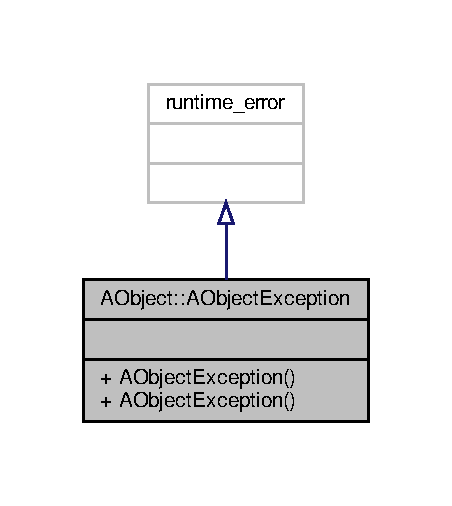
\includegraphics[width=217pt]{class_a_object_1_1_a_object_exception__inherit__graph}
\end{center}
\end{figure}


Collaboration diagram for A\+Object\+:\+:A\+Object\+Exception\+:
\nopagebreak
\begin{figure}[H]
\begin{center}
\leavevmode
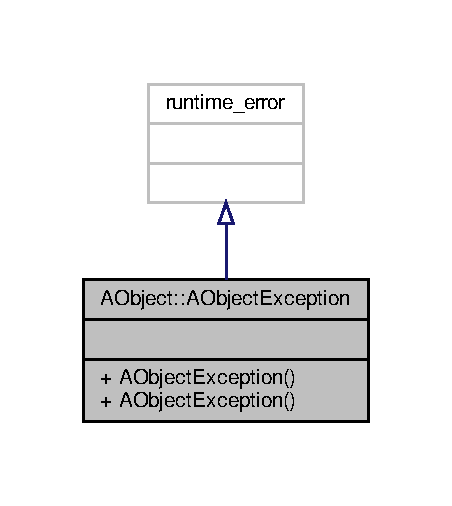
\includegraphics[width=217pt]{class_a_object_1_1_a_object_exception__coll__graph}
\end{center}
\end{figure}
\subsection*{Public Member Functions}
\begin{DoxyCompactItemize}
\item 
\mbox{\Hypertarget{class_a_object_1_1_a_object_exception_a92efc57e8b4aa4e9283b3bf124924908}\label{class_a_object_1_1_a_object_exception_a92efc57e8b4aa4e9283b3bf124924908}} 
\hyperlink{class_a_object_1_1_a_object_exception_a92efc57e8b4aa4e9283b3bf124924908}{A\+Object\+Exception} ()
\begin{DoxyCompactList}\small\item\em Construct a new \hyperlink{class_a_object_1_1_a_object_exception_a92efc57e8b4aa4e9283b3bf124924908}{A\+Object\+::\+A\+Object\+Exception\+::\+A\+Object\+Exception} object. \end{DoxyCompactList}\item 
\hyperlink{class_a_object_1_1_a_object_exception_a2c7e9151effc8e9b85500714fb1b87d6}{A\+Object\+Exception} (const char $\ast$what\+Arg)
\begin{DoxyCompactList}\small\item\em Construct a new \hyperlink{class_a_object_1_1_a_object_exception_a92efc57e8b4aa4e9283b3bf124924908}{A\+Object\+::\+A\+Object\+Exception\+::\+A\+Object\+Exception} object. \end{DoxyCompactList}\end{DoxyCompactItemize}


\subsection{Detailed Description}
\hyperlink{class_a_object}{A\+Object} Exception. 

\subsection{Constructor \& Destructor Documentation}
\mbox{\Hypertarget{class_a_object_1_1_a_object_exception_a2c7e9151effc8e9b85500714fb1b87d6}\label{class_a_object_1_1_a_object_exception_a2c7e9151effc8e9b85500714fb1b87d6}} 
\index{A\+Object\+::\+A\+Object\+Exception@{A\+Object\+::\+A\+Object\+Exception}!A\+Object\+Exception@{A\+Object\+Exception}}
\index{A\+Object\+Exception@{A\+Object\+Exception}!A\+Object\+::\+A\+Object\+Exception@{A\+Object\+::\+A\+Object\+Exception}}
\subsubsection{\texorpdfstring{A\+Object\+Exception()}{AObjectException()}}
{\footnotesize\ttfamily A\+Object\+::\+A\+Object\+Exception\+::\+A\+Object\+Exception (\begin{DoxyParamCaption}\item[{const char $\ast$}]{what\+Arg }\end{DoxyParamCaption})\hspace{0.3cm}{\ttfamily [explicit]}}



Construct a new \hyperlink{class_a_object_1_1_a_object_exception_a92efc57e8b4aa4e9283b3bf124924908}{A\+Object\+::\+A\+Object\+Exception\+::\+A\+Object\+Exception} object. 


\begin{DoxyParams}{Parameters}
{\em what\+Arg} & Error message \\
\hline
\end{DoxyParams}


The documentation for this class was generated from the following files\+:\begin{DoxyCompactItemize}
\item 
includes/A\+Object.\+hpp\item 
srcs/A\+Object.\+cpp\end{DoxyCompactItemize}

\hypertarget{class_a_scene}{}\doxysection{A\+Scene Class Reference}
\label{class_a_scene}\index{AScene@{AScene}}


base object to implement in all scenes  




{\ttfamily \#include $<$A\+Scene.\+hpp$>$}



Inheritance diagram for A\+Scene\+:
\nopagebreak
\begin{figure}[H]
\begin{center}
\leavevmode
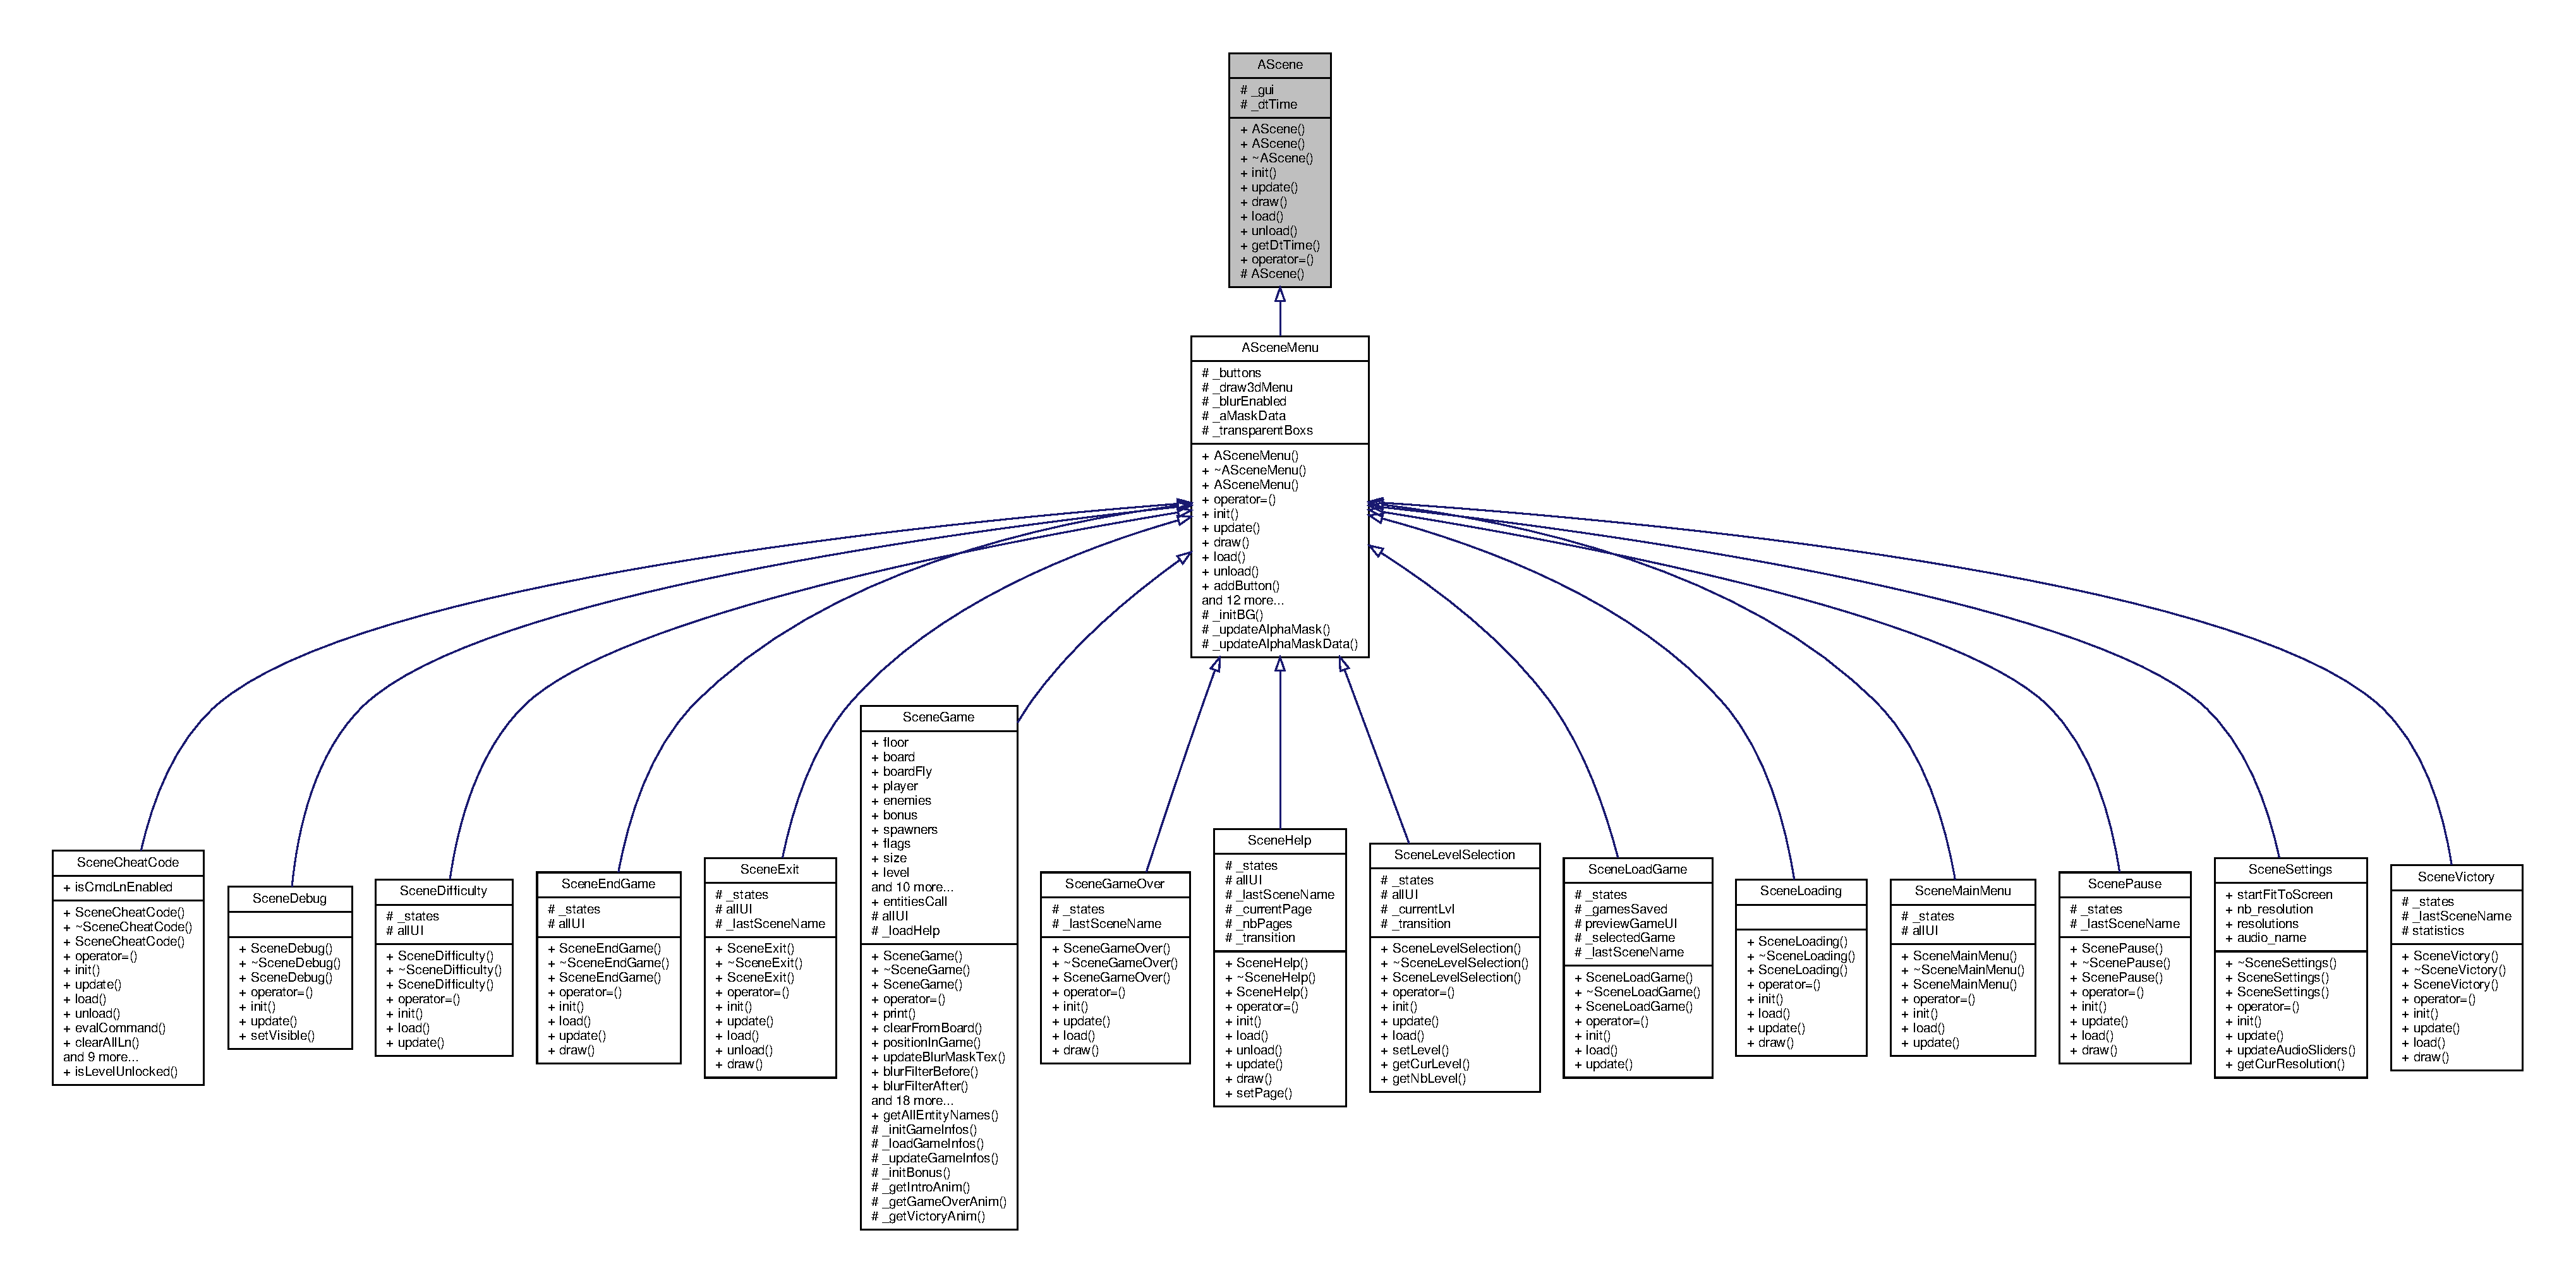
\includegraphics[width=350pt]{class_a_scene__inherit__graph}
\end{center}
\end{figure}


Collaboration diagram for A\+Scene\+:
\nopagebreak
\begin{figure}[H]
\begin{center}
\leavevmode
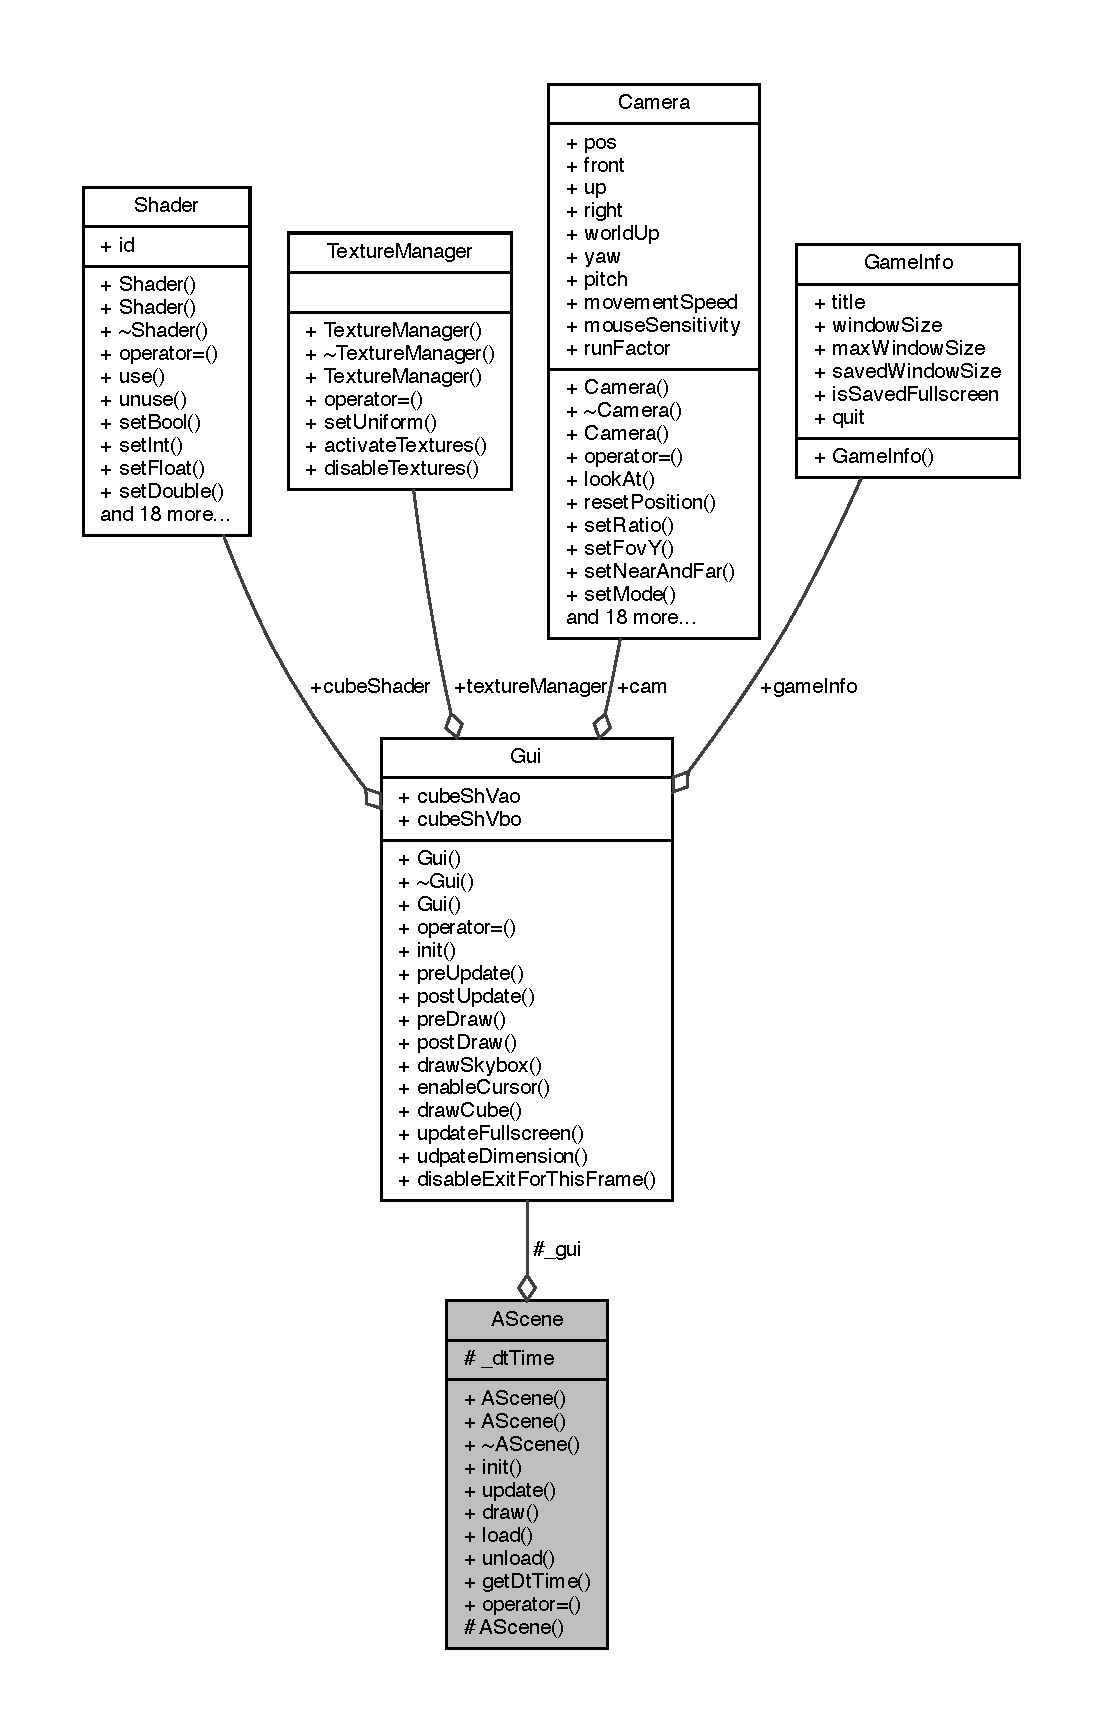
\includegraphics[width=350pt]{class_a_scene__coll__graph}
\end{center}
\end{figure}
\doxysubsection*{Classes}
\begin{DoxyCompactItemize}
\item 
class \mbox{\hyperlink{class_a_scene_1_1_scene_exception}{Scene\+Exception}}
\begin{DoxyCompactList}\small\item\em Scene exception. \end{DoxyCompactList}\end{DoxyCompactItemize}
\doxysubsection*{Public Member Functions}
\begin{DoxyCompactItemize}
\item 
\mbox{\hyperlink{class_a_scene_a00e7cd759bb0f43141df51c4ab6e6c47}{A\+Scene}} (\mbox{\hyperlink{class_gui}{Gui}} $\ast$gui, float const \&dt\+Time)
\begin{DoxyCompactList}\small\item\em Construct a new \mbox{\hyperlink{class_a_scene_a00e7cd759bb0f43141df51c4ab6e6c47}{A\+Scene\+::\+A\+Scene}} object. \end{DoxyCompactList}\item 
\mbox{\hyperlink{class_a_scene_aa204afecf39bdfcbe83dad3ed8cce34f}{A\+Scene}} (\mbox{\hyperlink{class_a_scene}{A\+Scene}} const \&src)
\begin{DoxyCompactList}\small\item\em Construct a new \mbox{\hyperlink{class_a_scene_a00e7cd759bb0f43141df51c4ab6e6c47}{A\+Scene\+::\+A\+Scene}} object. \end{DoxyCompactList}\item 
\mbox{\Hypertarget{class_a_scene_a9faf7f1a271327227e83627432d0b210}\label{class_a_scene_a9faf7f1a271327227e83627432d0b210}} 
virtual \mbox{\hyperlink{class_a_scene_a9faf7f1a271327227e83627432d0b210}{$\sim$\+A\+Scene}} ()
\begin{DoxyCompactList}\small\item\em Destroy the \mbox{\hyperlink{class_a_scene_a00e7cd759bb0f43141df51c4ab6e6c47}{A\+Scene\+::\+A\+Scene}} object. \end{DoxyCompactList}\item 
virtual bool \mbox{\hyperlink{class_a_scene_ad431efa9c183182e8b5abb1bb8437a74}{init}} ()=0
\begin{DoxyCompactList}\small\item\em Init the scene. \end{DoxyCompactList}\item 
virtual bool \mbox{\hyperlink{class_a_scene_af3ed61809cc5924b9d5530473576a0c7}{update}} ()=0
\begin{DoxyCompactList}\small\item\em Update the scene (called every frames) \end{DoxyCompactList}\item 
virtual bool \mbox{\hyperlink{class_a_scene_a7c303489d4c296482af38aa5deccbd8b}{draw}} ()=0
\begin{DoxyCompactList}\small\item\em Draw the scene (called every frames) \end{DoxyCompactList}\item 
\mbox{\Hypertarget{class_a_scene_a8f6201c6a7ccefdebdc9ecf69d35a1d8}\label{class_a_scene_a8f6201c6a7ccefdebdc9ecf69d35a1d8}} 
virtual void \mbox{\hyperlink{class_a_scene_a8f6201c6a7ccefdebdc9ecf69d35a1d8}{load}} ()=0
\begin{DoxyCompactList}\small\item\em Load the scene (called on every scene loading) \end{DoxyCompactList}\item 
\mbox{\Hypertarget{class_a_scene_aeb259110cc48bac42ea05bbe24b5d2a8}\label{class_a_scene_aeb259110cc48bac42ea05bbe24b5d2a8}} 
virtual void \mbox{\hyperlink{class_a_scene_aeb259110cc48bac42ea05bbe24b5d2a8}{unload}} ()=0
\begin{DoxyCompactList}\small\item\em Unload the scene (called on every scene unloading) \end{DoxyCompactList}\item 
float const  \& \mbox{\hyperlink{class_a_scene_aad3e0d8810515e904fc315a12a344bc3}{get\+Dt\+Time}} () const
\begin{DoxyCompactList}\small\item\em Get the delta time. \end{DoxyCompactList}\item 
\mbox{\hyperlink{class_a_scene}{A\+Scene}} \& \mbox{\hyperlink{class_a_scene_aedf714310c418b3972e2e9c96ac7bff1}{operator=}} (\mbox{\hyperlink{class_a_scene}{A\+Scene}} const \&rhs)
\begin{DoxyCompactList}\small\item\em Copy this object. \end{DoxyCompactList}\end{DoxyCompactItemize}
\doxysubsection*{Protected Attributes}
\begin{DoxyCompactItemize}
\item 
\mbox{\hyperlink{class_gui}{Gui}} $\ast$ \mbox{\hyperlink{class_a_scene_afdf549ea35306aecfa7a7976a5594fe1}{\+\_\+gui}}
\item 
float const  \& \mbox{\hyperlink{class_a_scene_a8cbb61bc0c24add293a08d3cc83ac2ea}{\+\_\+dt\+Time}}
\end{DoxyCompactItemize}


\doxysubsection{Detailed Description}
base object to implement in all scenes 

\doxysubsection{Constructor \& Destructor Documentation}
\mbox{\Hypertarget{class_a_scene_a00e7cd759bb0f43141df51c4ab6e6c47}\label{class_a_scene_a00e7cd759bb0f43141df51c4ab6e6c47}} 
\index{AScene@{AScene}!AScene@{AScene}}
\index{AScene@{AScene}!AScene@{AScene}}
\doxysubsubsection{\texorpdfstring{AScene()}{AScene()}\hspace{0.1cm}{\footnotesize\ttfamily [1/2]}}
{\footnotesize\ttfamily A\+Scene\+::\+A\+Scene (\begin{DoxyParamCaption}\item[{\mbox{\hyperlink{class_gui}{Gui}} $\ast$}]{gui,  }\item[{float const \&}]{dt\+Time }\end{DoxyParamCaption})}



Construct a new \mbox{\hyperlink{class_a_scene_a00e7cd759bb0f43141df51c4ab6e6c47}{A\+Scene\+::\+A\+Scene}} object. 


\begin{DoxyParams}{Parameters}
{\em gui} & A pointer on the gui object \\
\hline
{\em dt\+Time} & A reference to the delta time \\
\hline
\end{DoxyParams}
\mbox{\Hypertarget{class_a_scene_aa204afecf39bdfcbe83dad3ed8cce34f}\label{class_a_scene_aa204afecf39bdfcbe83dad3ed8cce34f}} 
\index{AScene@{AScene}!AScene@{AScene}}
\index{AScene@{AScene}!AScene@{AScene}}
\doxysubsubsection{\texorpdfstring{AScene()}{AScene()}\hspace{0.1cm}{\footnotesize\ttfamily [2/2]}}
{\footnotesize\ttfamily A\+Scene\+::\+A\+Scene (\begin{DoxyParamCaption}\item[{\mbox{\hyperlink{class_a_scene}{A\+Scene}} const \&}]{src }\end{DoxyParamCaption})}



Construct a new \mbox{\hyperlink{class_a_scene_a00e7cd759bb0f43141df51c4ab6e6c47}{A\+Scene\+::\+A\+Scene}} object. 


\begin{DoxyParams}{Parameters}
{\em src} & The object to do the copy \\
\hline
\end{DoxyParams}


\doxysubsection{Member Function Documentation}
\mbox{\Hypertarget{class_a_scene_a7c303489d4c296482af38aa5deccbd8b}\label{class_a_scene_a7c303489d4c296482af38aa5deccbd8b}} 
\index{AScene@{AScene}!draw@{draw}}
\index{draw@{draw}!AScene@{AScene}}
\doxysubsubsection{\texorpdfstring{draw()}{draw()}}
{\footnotesize\ttfamily virtual bool A\+Scene\+::draw (\begin{DoxyParamCaption}{ }\end{DoxyParamCaption})\hspace{0.3cm}{\ttfamily [pure virtual]}}



Draw the scene (called every frames) 

\begin{DoxyReturn}{Returns}
false If failed 
\end{DoxyReturn}


Implemented in \mbox{\hyperlink{class_scene_game_a0797fee2de442f68aef19cc5c3299ec3}{Scene\+Game}}, \mbox{\hyperlink{class_a_scene_menu_a5c11f34c83f025e1181219bf25ce4694}{A\+Scene\+Menu}}, \mbox{\hyperlink{class_scene_help_a8f6cc7a52fe41d06815ff10a9ac941a2}{Scene\+Help}}, \mbox{\hyperlink{class_scene_end_game_a145614d80f41512a5bcf539278555d0c}{Scene\+End\+Game}}, \mbox{\hyperlink{class_scene_exit_a3b7110e736f86836568fdb2f8a997877}{Scene\+Exit}}, \mbox{\hyperlink{class_scene_loading_ae51a1b4d4f738847d50036c174364f9e}{Scene\+Loading}}, \mbox{\hyperlink{class_scene_game_over_aa9c4f9d3cabdc89176c0113e2864f3e8}{Scene\+Game\+Over}}, \mbox{\hyperlink{class_scene_pause_aa59d21ea311bab5163574441f3960734}{Scene\+Pause}}, and \mbox{\hyperlink{class_scene_victory_ac79e3eadfb4bfafa8733888a1e86f57e}{Scene\+Victory}}.

\mbox{\Hypertarget{class_a_scene_aad3e0d8810515e904fc315a12a344bc3}\label{class_a_scene_aad3e0d8810515e904fc315a12a344bc3}} 
\index{AScene@{AScene}!getDtTime@{getDtTime}}
\index{getDtTime@{getDtTime}!AScene@{AScene}}
\doxysubsubsection{\texorpdfstring{getDtTime()}{getDtTime()}}
{\footnotesize\ttfamily float const  \& A\+Scene\+::get\+Dt\+Time (\begin{DoxyParamCaption}{ }\end{DoxyParamCaption}) const}



Get the delta time. 

\begin{DoxyReturn}{Returns}
float const\& The delta time 
\end{DoxyReturn}
\mbox{\Hypertarget{class_a_scene_ad431efa9c183182e8b5abb1bb8437a74}\label{class_a_scene_ad431efa9c183182e8b5abb1bb8437a74}} 
\index{AScene@{AScene}!init@{init}}
\index{init@{init}!AScene@{AScene}}
\doxysubsubsection{\texorpdfstring{init()}{init()}}
{\footnotesize\ttfamily virtual bool A\+Scene\+::init (\begin{DoxyParamCaption}{ }\end{DoxyParamCaption})\hspace{0.3cm}{\ttfamily [pure virtual]}}



Init the scene. 

\begin{DoxyReturn}{Returns}
false If failed 
\end{DoxyReturn}


Implemented in \mbox{\hyperlink{class_a_scene_menu_a78bdee98bd7df224524586a060f9bdec}{A\+Scene\+Menu}}, \mbox{\hyperlink{class_scene_game_a841268ba3ea129f7c02cfafcafd32a4f}{Scene\+Game}}, \mbox{\hyperlink{class_scene_cheat_code_aa952941065350cdde0390695b32ac31d}{Scene\+Cheat\+Code}}, \mbox{\hyperlink{class_scene_settings_a19323950409add2d1b0df92799acf4d2}{Scene\+Settings}}, \mbox{\hyperlink{class_scene_debug_a4e413808e3d50dd29f9e1d07df4e6c4c}{Scene\+Debug}}, \mbox{\hyperlink{class_scene_help_adabf402b245092d311b08ec1139aa3c5}{Scene\+Help}}, \mbox{\hyperlink{class_scene_level_selection_ab6374f18220f26c22e062bfacc2ff962}{Scene\+Level\+Selection}}, \mbox{\hyperlink{class_scene_difficulty_a7fb9dd5ee9d623e346d917cd7a5db956}{Scene\+Difficulty}}, \mbox{\hyperlink{class_scene_end_game_a9503a63d52d2a11dbc56c97f35ff6eae}{Scene\+End\+Game}}, \mbox{\hyperlink{class_scene_loading_aa0463a9826f1b50e5980e41d57c80778}{Scene\+Loading}}, \mbox{\hyperlink{class_scene_main_menu_a11f68db49f9bf996efb0ce14913e5580}{Scene\+Main\+Menu}}, \mbox{\hyperlink{class_scene_exit_ad9168291bb031fee797a7964590e1b73}{Scene\+Exit}}, \mbox{\hyperlink{class_scene_game_over_a7ddd370503e10ff64e3d023f0a0acdb8}{Scene\+Game\+Over}}, \mbox{\hyperlink{class_scene_load_game_a4ef89351e679b7f681fa55e5f723dd16}{Scene\+Load\+Game}}, \mbox{\hyperlink{class_scene_pause_ae5e00c5fcd82e97985d93f918b9e4b35}{Scene\+Pause}}, and \mbox{\hyperlink{class_scene_victory_ab7dc4308732478fa13c8a3209f63e6b7}{Scene\+Victory}}.

\mbox{\Hypertarget{class_a_scene_aedf714310c418b3972e2e9c96ac7bff1}\label{class_a_scene_aedf714310c418b3972e2e9c96ac7bff1}} 
\index{AScene@{AScene}!operator=@{operator=}}
\index{operator=@{operator=}!AScene@{AScene}}
\doxysubsubsection{\texorpdfstring{operator=()}{operator=()}}
{\footnotesize\ttfamily \mbox{\hyperlink{class_a_scene}{A\+Scene}} \& A\+Scene\+::operator= (\begin{DoxyParamCaption}\item[{\mbox{\hyperlink{class_a_scene}{A\+Scene}} const \&}]{rhs }\end{DoxyParamCaption})}



Copy this object. 


\begin{DoxyParams}{Parameters}
{\em rhs} & The object to copy \\
\hline
\end{DoxyParams}
\begin{DoxyReturn}{Returns}
\mbox{\hyperlink{class_a_scene}{A\+Scene}}\& A reference to the copied object 
\end{DoxyReturn}
\mbox{\Hypertarget{class_a_scene_af3ed61809cc5924b9d5530473576a0c7}\label{class_a_scene_af3ed61809cc5924b9d5530473576a0c7}} 
\index{AScene@{AScene}!update@{update}}
\index{update@{update}!AScene@{AScene}}
\doxysubsubsection{\texorpdfstring{update()}{update()}}
{\footnotesize\ttfamily virtual bool A\+Scene\+::update (\begin{DoxyParamCaption}{ }\end{DoxyParamCaption})\hspace{0.3cm}{\ttfamily [pure virtual]}}



Update the scene (called every frames) 

\begin{DoxyReturn}{Returns}
false If failed 
\end{DoxyReturn}


Implemented in \mbox{\hyperlink{class_scene_game_a5e23048e3ad8c6fde2d753ed7449e2d5}{Scene\+Game}}, \mbox{\hyperlink{class_scene_cheat_code_ab6ae0c8b3adbce736429e61a27966e31}{Scene\+Cheat\+Code}}, \mbox{\hyperlink{class_scene_settings_ac32c443d620d0417b301193e87885a91}{Scene\+Settings}}, \mbox{\hyperlink{class_a_scene_menu_a1deeb5fd9be97376998cd2af36f29744}{A\+Scene\+Menu}}, \mbox{\hyperlink{class_scene_debug_a97234cec6e43aa3d891e3f6d2ff51528}{Scene\+Debug}}, \mbox{\hyperlink{class_scene_help_aa5170e0722a6aecbfeea1f920d09cff7}{Scene\+Help}}, \mbox{\hyperlink{class_scene_difficulty_a2a3d3328b04df7047cc03725a9c5eb3c}{Scene\+Difficulty}}, \mbox{\hyperlink{class_scene_end_game_a36b55558e75b9cad9d17a28d8a1ce8d2}{Scene\+End\+Game}}, \mbox{\hyperlink{class_scene_level_selection_a9784885da4583eaba695812bedf8847c}{Scene\+Level\+Selection}}, \mbox{\hyperlink{class_scene_loading_a5b4f2b636e55908bb2f29180aa875201}{Scene\+Loading}}, \mbox{\hyperlink{class_scene_main_menu_a5d095883d0b1fceb3125ef2689a7a09c}{Scene\+Main\+Menu}}, \mbox{\hyperlink{class_scene_load_game_ad33de3b5d98596754f058a4e096ba1b3}{Scene\+Load\+Game}}, \mbox{\hyperlink{class_scene_exit_a60fd49ea48551bd3035efa7cabe4d08d}{Scene\+Exit}}, \mbox{\hyperlink{class_scene_game_over_ac4547b0ed87f3c324e75dafb8f96b5af}{Scene\+Game\+Over}}, \mbox{\hyperlink{class_scene_pause_a376de6952be83718fb19d268d9327ef6}{Scene\+Pause}}, and \mbox{\hyperlink{class_scene_victory_aea51a7b48a3243175e1759b20f853c16}{Scene\+Victory}}.



\doxysubsection{Member Data Documentation}
\mbox{\Hypertarget{class_a_scene_a8cbb61bc0c24add293a08d3cc83ac2ea}\label{class_a_scene_a8cbb61bc0c24add293a08d3cc83ac2ea}} 
\index{AScene@{AScene}!\_dtTime@{\_dtTime}}
\index{\_dtTime@{\_dtTime}!AScene@{AScene}}
\doxysubsubsection{\texorpdfstring{\_dtTime}{\_dtTime}}
{\footnotesize\ttfamily float const\& A\+Scene\+::\+\_\+dt\+Time\hspace{0.3cm}{\ttfamily [protected]}}

A reference to the delta time \mbox{\Hypertarget{class_a_scene_afdf549ea35306aecfa7a7976a5594fe1}\label{class_a_scene_afdf549ea35306aecfa7a7976a5594fe1}} 
\index{AScene@{AScene}!\_gui@{\_gui}}
\index{\_gui@{\_gui}!AScene@{AScene}}
\doxysubsubsection{\texorpdfstring{\_gui}{\_gui}}
{\footnotesize\ttfamily \mbox{\hyperlink{class_gui}{Gui}}$\ast$ A\+Scene\+::\+\_\+gui\hspace{0.3cm}{\ttfamily [protected]}}

A reference to the gui object 

The documentation for this class was generated from the following files\+:\begin{DoxyCompactItemize}
\item 
includes/scenes/A\+Scene.\+hpp\item 
srcs/scenes/A\+Scene.\+cpp\end{DoxyCompactItemize}

\hypertarget{class_a_scene_menu}{}\doxysection{A\+Scene\+Menu Class Reference}
\label{class_a_scene_menu}\index{ASceneMenu@{ASceneMenu}}


Scene object to re-\/implement in all scenes for menu.  




{\ttfamily \#include $<$A\+Scene\+Menu.\+hpp$>$}



Inheritance diagram for A\+Scene\+Menu\+:\nopagebreak
\begin{figure}[H]
\begin{center}
\leavevmode
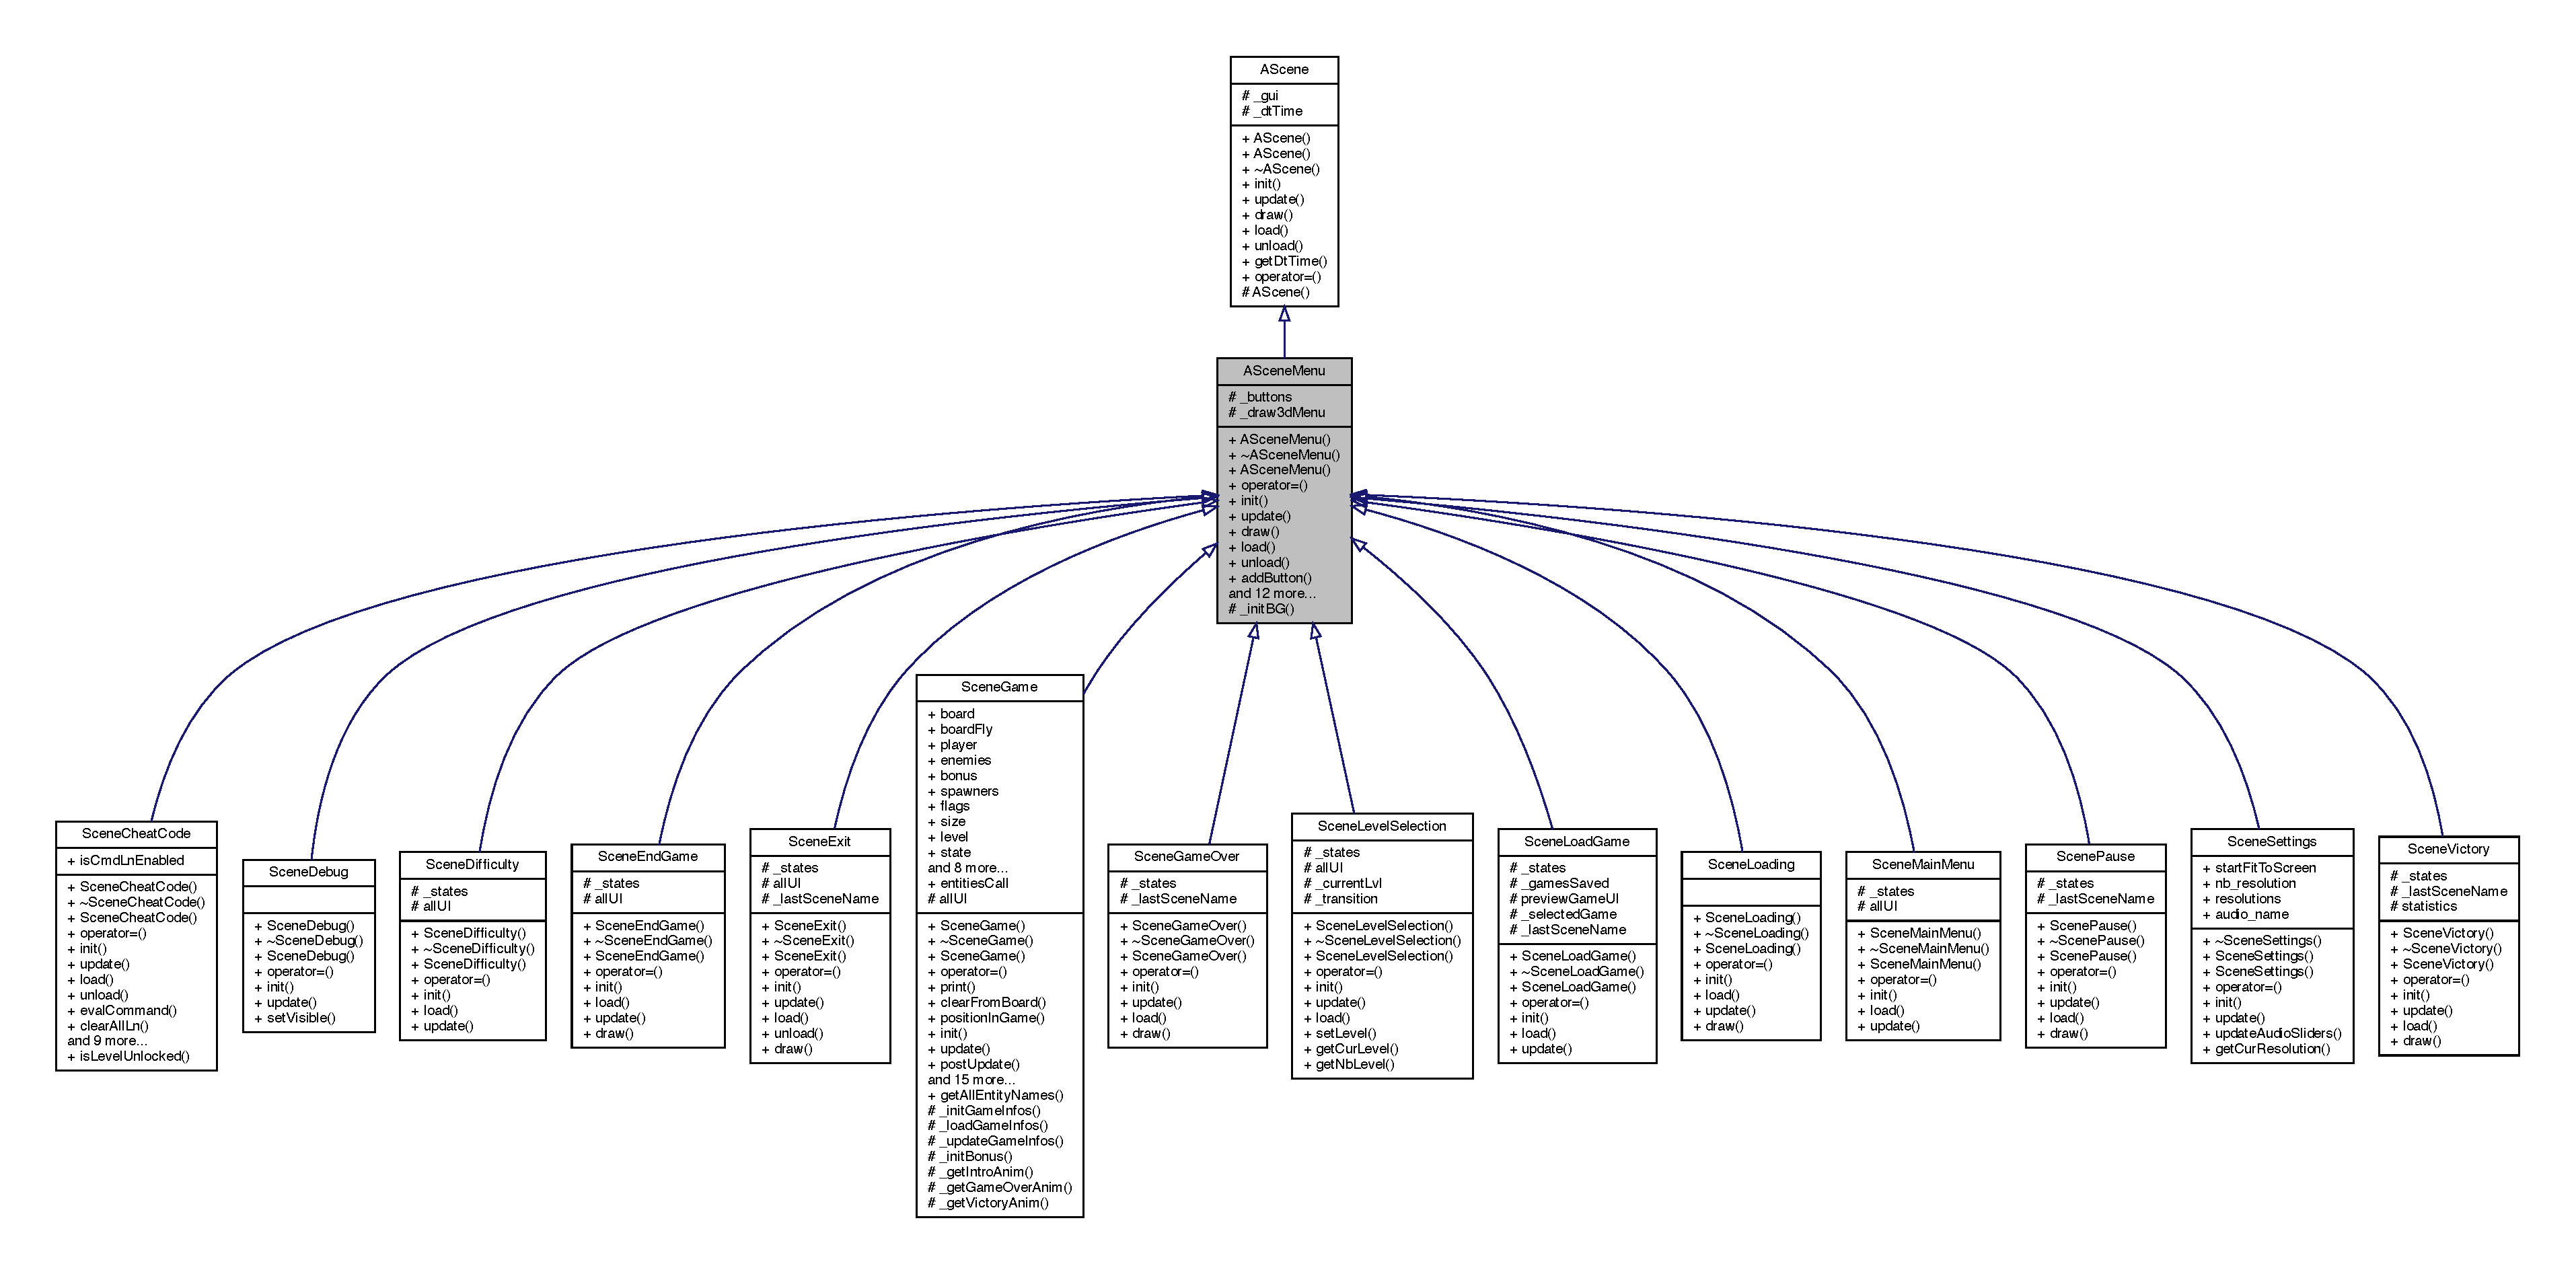
\includegraphics[width=350pt]{class_a_scene_menu__inherit__graph}
\end{center}
\end{figure}


Collaboration diagram for A\+Scene\+Menu\+:\nopagebreak
\begin{figure}[H]
\begin{center}
\leavevmode
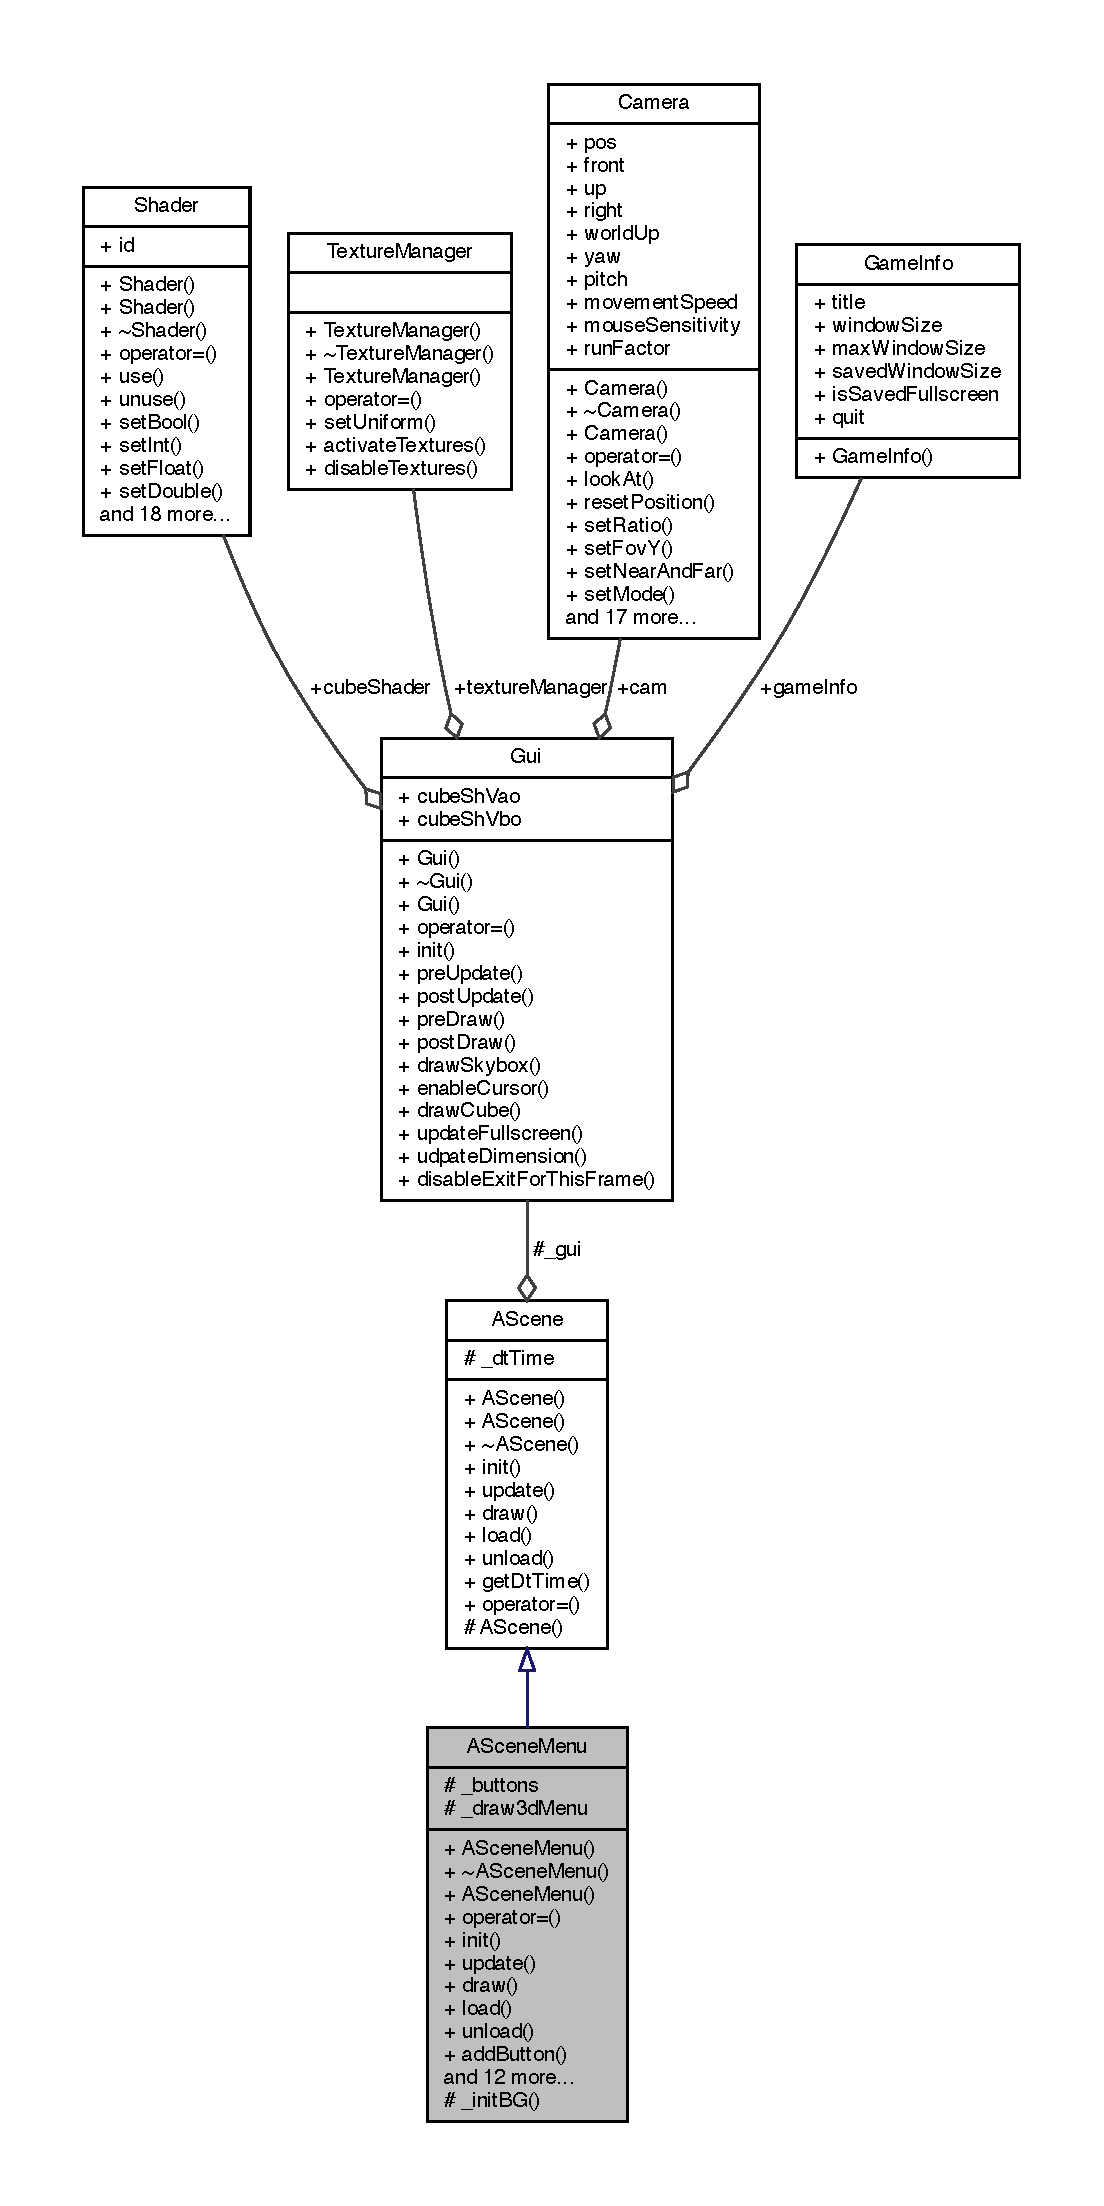
\includegraphics[height=550pt]{class_a_scene_menu__coll__graph}
\end{center}
\end{figure}
\doxysubsection*{Public Member Functions}
\begin{DoxyCompactItemize}
\item 
\mbox{\Hypertarget{class_a_scene_menu_a97a8137c54f33e8f08adde2c2bb604c6}\label{class_a_scene_menu_a97a8137c54f33e8f08adde2c2bb604c6}} 
{\bfseries A\+Scene\+Menu} (\mbox{\hyperlink{class_gui}{Gui}} $\ast$gui, float const \&dt\+Time)
\item 
\mbox{\Hypertarget{class_a_scene_menu_a9962aa28c98e9471256c494563457f4b}\label{class_a_scene_menu_a9962aa28c98e9471256c494563457f4b}} 
{\bfseries A\+Scene\+Menu} (\mbox{\hyperlink{class_a_scene_menu}{A\+Scene\+Menu}} const \&src)
\item 
\mbox{\Hypertarget{class_a_scene_menu_a3e4fc24a1fb0bcd6296f4856a2e3c611}\label{class_a_scene_menu_a3e4fc24a1fb0bcd6296f4856a2e3c611}} 
\mbox{\hyperlink{class_a_scene_menu}{A\+Scene\+Menu}} \& {\bfseries operator=} (\mbox{\hyperlink{class_a_scene_menu}{A\+Scene\+Menu}} const \&rhs)
\item 
\mbox{\Hypertarget{class_a_scene_menu_a78bdee98bd7df224524586a060f9bdec}\label{class_a_scene_menu_a78bdee98bd7df224524586a060f9bdec}} 
virtual bool {\bfseries init} ()=0
\item 
virtual bool \mbox{\hyperlink{class_a_scene_menu_a1deeb5fd9be97376998cd2af36f29744}{update}} ()
\begin{DoxyCompactList}\small\item\em this is the update function (called every frames) \end{DoxyCompactList}\item 
virtual bool \mbox{\hyperlink{class_a_scene_menu_a5c11f34c83f025e1181219bf25ce4694}{draw}} ()
\begin{DoxyCompactList}\small\item\em this is the draw function (called every frames) \end{DoxyCompactList}\item 
\mbox{\Hypertarget{class_a_scene_menu_a85a4451f4fb6a3ae7a66f1296800d11e}\label{class_a_scene_menu_a85a4451f4fb6a3ae7a66f1296800d11e}} 
virtual void \mbox{\hyperlink{class_a_scene_menu_a85a4451f4fb6a3ae7a66f1296800d11e}{load}} ()
\begin{DoxyCompactList}\small\item\em called when the scene is loaded \end{DoxyCompactList}\item 
\mbox{\Hypertarget{class_a_scene_menu_ad493937ca0d8ec4d710307593c0e77c1}\label{class_a_scene_menu_ad493937ca0d8ec4d710307593c0e77c1}} 
virtual void \mbox{\hyperlink{class_a_scene_menu_ad493937ca0d8ec4d710307593c0e77c1}{unload}} ()
\begin{DoxyCompactList}\small\item\em called when the scene is unloaded \end{DoxyCompactList}\item 
\mbox{\hyperlink{class_button_u_i}{Button\+UI}} \& \mbox{\hyperlink{class_a_scene_menu_a20622fb8d15a21b407d4832e66162cbb}{add\+Button}} (glm\+::vec2 pos, glm\+::vec2 size, std\+::string const \&text)
\begin{DoxyCompactList}\small\item\em add a button in the menu with menu settings \end{DoxyCompactList}\item 
\mbox{\hyperlink{class_button_image_u_i}{Button\+Image\+UI}} \& \mbox{\hyperlink{class_a_scene_menu_a0c777fee34873f9528c8beb08aa2eca6}{add\+Button\+Image}} (glm\+::vec2 pos, glm\+::vec2 size, std\+::string const \&filename)
\begin{DoxyCompactList}\small\item\em add a button with image in the menu with menu settings \end{DoxyCompactList}\item 
\mbox{\hyperlink{class_slider_u_i}{Slider\+UI}} \& \mbox{\hyperlink{class_a_scene_menu_ad526697a433c9f8e627eb6c147a5bd20}{add\+Slider}} (glm\+::vec2 pos, glm\+::vec2 size, float min, float max, float val, float step)
\begin{DoxyCompactList}\small\item\em add a slider in the menu with menu settings \end{DoxyCompactList}\item 
\mbox{\hyperlink{class_text_u_i}{Text\+UI}} \& \mbox{\hyperlink{class_a_scene_menu_a209b1c4974690a8070835772b3b008b0}{add\+Text}} (glm\+::vec2 pos, glm\+::vec2 size, std\+::string const \&text)
\begin{DoxyCompactList}\small\item\em add a text in the menu with menu settings \end{DoxyCompactList}\item 
\mbox{\hyperlink{class_text_u_i}{Text\+UI}} \& \mbox{\hyperlink{class_a_scene_menu_a35ca98e36b71c2915771a5878ecea077}{add\+Title}} (glm\+::vec2 pos, glm\+::vec2 size, std\+::string const \&text)
\begin{DoxyCompactList}\small\item\em add a Title in the menu with menu settings \end{DoxyCompactList}\item 
\mbox{\hyperlink{class_rect_u_i}{Rect\+UI}} \& \mbox{\hyperlink{class_a_scene_menu_abbada4b933b8b6fa9135a143acc8198d}{add\+Rect}} (glm\+::vec2 pos, glm\+::vec2 size, glm\+::vec4 color=V\+O\+I\+D\+\_\+\+C\+O\+L\+OR, glm\+::vec4 border\+Color=V\+O\+I\+D\+\_\+\+C\+O\+L\+OR)
\begin{DoxyCompactList}\small\item\em add a rectange in the menu with menu settings \end{DoxyCompactList}\item 
\mbox{\hyperlink{class_image_u_i}{Image\+UI}} \& \mbox{\hyperlink{class_a_scene_menu_a4476a757ca150acf6ae85a3e64e65558}{add\+Image}} (glm\+::vec2 pos, glm\+::vec2 size, std\+::string const \&filename)
\begin{DoxyCompactList}\small\item\em add an image in the menu with menu settings \end{DoxyCompactList}\item 
\mbox{\hyperlink{class_scrollbar_u_i}{Scrollbar\+UI}} \& \mbox{\hyperlink{class_a_scene_menu_a9330a0a513fc803057b8b6fb65bfd954}{add\+Scrollbar}} (glm\+::vec2 pos, glm\+::vec2 size)
\begin{DoxyCompactList}\small\item\em add a scrollbar in the menu with menu settings \end{DoxyCompactList}\item 
\mbox{\hyperlink{class_empty_master_u_i}{Empty\+Master\+UI}} \& \mbox{\hyperlink{class_a_scene_menu_a59dfc339cc860204011104cb6598162c}{add\+Empty\+Master}} ()
\begin{DoxyCompactList}\small\item\em add an empty master object on the total screen in the menu with menu settings \end{DoxyCompactList}\item 
\mbox{\hyperlink{class_text_input_u_i}{Text\+Input\+UI}} \& \mbox{\hyperlink{class_a_scene_menu_a17b4546a13c714760dbc18f496361bc3}{add\+Text\+Input}} (glm\+::vec2 pos, glm\+::vec2 size, std\+::string const \&def\+Text)
\begin{DoxyCompactList}\small\item\em add a text\+Input in the menu with menu settings \end{DoxyCompactList}\item 
\mbox{\hyperlink{class_button_image_u_i}{Button\+Image\+UI}} \& \mbox{\hyperlink{class_a_scene_menu_ac1883fd509d5ac2306e009bd2cead752}{add\+Exit\+Button}} ()
\begin{DoxyCompactList}\small\item\em Add an exit button on the screen. \end{DoxyCompactList}\item 
\mbox{\Hypertarget{class_a_scene_menu_a251ef83adb546bb22915f52986bc7d84}\label{class_a_scene_menu_a251ef83adb546bb22915f52986bc7d84}} 
\mbox{\hyperlink{class_a_base_u_i}{A\+Base\+UI}} \& {\bfseries get\+U\+I\+Element} (uint32\+\_\+t id)
\item 
\mbox{\Hypertarget{class_a_scene_menu_a13b29d13f531109e90428c6f14d50e05}\label{class_a_scene_menu_a13b29d13f531109e90428c6f14d50e05}} 
uint32\+\_\+t {\bfseries get\+Nb\+U\+I\+Elements} () const
\end{DoxyCompactItemize}
\doxysubsection*{Protected Member Functions}
\begin{DoxyCompactItemize}
\item 
bool \mbox{\hyperlink{class_a_scene_menu_aa54bec80fcc36b1607eeb1bb80ab0142}{\+\_\+init\+BG}} ()
\begin{DoxyCompactList}\small\item\em init the basic background of the menu \end{DoxyCompactList}\end{DoxyCompactItemize}
\doxysubsection*{Protected Attributes}
\begin{DoxyCompactItemize}
\item 
\mbox{\Hypertarget{class_a_scene_menu_ae18fa3a41aef71fd11a3166221b69024}\label{class_a_scene_menu_ae18fa3a41aef71fd11a3166221b69024}} 
std\+::vector$<$ \mbox{\hyperlink{class_a_base_u_i}{A\+Base\+UI}} $\ast$ $>$ {\bfseries \+\_\+buttons}
\item 
\mbox{\Hypertarget{class_a_scene_menu_a10b81e94fdaeb7d466279db7c184d8f9}\label{class_a_scene_menu_a10b81e94fdaeb7d466279db7c184d8f9}} 
bool {\bfseries \+\_\+draw3d\+Menu}
\end{DoxyCompactItemize}
\doxysubsection*{Friends}
\begin{DoxyCompactItemize}
\item 
\mbox{\Hypertarget{class_a_scene_menu_a402599a9f1ae99fd18976f6f3616fcc1}\label{class_a_scene_menu_a402599a9f1ae99fd18976f6f3616fcc1}} 
std\+::ostream \& {\bfseries operator$<$$<$} (std\+::ostream \&os, const \mbox{\hyperlink{class_a_scene_menu}{A\+Scene\+Menu}} \&my\+Class)
\end{DoxyCompactItemize}


\doxysubsection{Detailed Description}
Scene object to re-\/implement in all scenes for menu. 

this object contains functions to create buttons, images, ... 

\doxysubsection{Member Function Documentation}
\mbox{\Hypertarget{class_a_scene_menu_aa54bec80fcc36b1607eeb1bb80ab0142}\label{class_a_scene_menu_aa54bec80fcc36b1607eeb1bb80ab0142}} 
\index{ASceneMenu@{ASceneMenu}!\_initBG@{\_initBG}}
\index{\_initBG@{\_initBG}!ASceneMenu@{ASceneMenu}}
\doxysubsubsection{\texorpdfstring{\_initBG()}{\_initBG()}}
{\footnotesize\ttfamily bool A\+Scene\+Menu\+::\+\_\+init\+BG (\begin{DoxyParamCaption}{ }\end{DoxyParamCaption})\hspace{0.3cm}{\ttfamily [protected]}}



init the basic background of the menu 

\begin{DoxyReturn}{Returns}
true if success 

false if error 
\end{DoxyReturn}
\mbox{\Hypertarget{class_a_scene_menu_a20622fb8d15a21b407d4832e66162cbb}\label{class_a_scene_menu_a20622fb8d15a21b407d4832e66162cbb}} 
\index{ASceneMenu@{ASceneMenu}!addButton@{addButton}}
\index{addButton@{addButton}!ASceneMenu@{ASceneMenu}}
\doxysubsubsection{\texorpdfstring{addButton()}{addButton()}}
{\footnotesize\ttfamily \mbox{\hyperlink{class_button_u_i}{Button\+UI}} \& A\+Scene\+Menu\+::add\+Button (\begin{DoxyParamCaption}\item[{glm\+::vec2}]{pos,  }\item[{glm\+::vec2}]{size,  }\item[{std\+::string const \&}]{text }\end{DoxyParamCaption})}



add a button in the menu with menu settings 


\begin{DoxyParams}{Parameters}
{\em pos} & the position \\
\hline
{\em size} & the size \\
\hline
{\em text} & the text in the button \\
\hline
\end{DoxyParams}
\begin{DoxyReturn}{Returns}
\mbox{\hyperlink{class_button_u_i}{Button\+UI}}\& a reference to the element created 
\end{DoxyReturn}
\mbox{\Hypertarget{class_a_scene_menu_a0c777fee34873f9528c8beb08aa2eca6}\label{class_a_scene_menu_a0c777fee34873f9528c8beb08aa2eca6}} 
\index{ASceneMenu@{ASceneMenu}!addButtonImage@{addButtonImage}}
\index{addButtonImage@{addButtonImage}!ASceneMenu@{ASceneMenu}}
\doxysubsubsection{\texorpdfstring{addButtonImage()}{addButtonImage()}}
{\footnotesize\ttfamily \mbox{\hyperlink{class_button_image_u_i}{Button\+Image\+UI}} \& A\+Scene\+Menu\+::add\+Button\+Image (\begin{DoxyParamCaption}\item[{glm\+::vec2}]{pos,  }\item[{glm\+::vec2}]{size,  }\item[{std\+::string const \&}]{filename }\end{DoxyParamCaption})}



add a button with image in the menu with menu settings 


\begin{DoxyParams}{Parameters}
{\em pos} & the position \\
\hline
{\em size} & the size \\
\hline
{\em filename} & the path to the image \\
\hline
\end{DoxyParams}
\begin{DoxyReturn}{Returns}
\mbox{\hyperlink{class_button_image_u_i}{Button\+Image\+UI}}\& a reference to the element created 
\end{DoxyReturn}
\mbox{\Hypertarget{class_a_scene_menu_a59dfc339cc860204011104cb6598162c}\label{class_a_scene_menu_a59dfc339cc860204011104cb6598162c}} 
\index{ASceneMenu@{ASceneMenu}!addEmptyMaster@{addEmptyMaster}}
\index{addEmptyMaster@{addEmptyMaster}!ASceneMenu@{ASceneMenu}}
\doxysubsubsection{\texorpdfstring{addEmptyMaster()}{addEmptyMaster()}}
{\footnotesize\ttfamily \mbox{\hyperlink{class_empty_master_u_i}{Empty\+Master\+UI}} \& A\+Scene\+Menu\+::add\+Empty\+Master (\begin{DoxyParamCaption}{ }\end{DoxyParamCaption})}



add an empty master object on the total screen in the menu with menu settings 

\begin{DoxyReturn}{Returns}
\mbox{\hyperlink{class_scrollbar_u_i}{Scrollbar\+UI}}\& a reference to the element created 
\end{DoxyReturn}
\mbox{\Hypertarget{class_a_scene_menu_ac1883fd509d5ac2306e009bd2cead752}\label{class_a_scene_menu_ac1883fd509d5ac2306e009bd2cead752}} 
\index{ASceneMenu@{ASceneMenu}!addExitButton@{addExitButton}}
\index{addExitButton@{addExitButton}!ASceneMenu@{ASceneMenu}}
\doxysubsubsection{\texorpdfstring{addExitButton()}{addExitButton()}}
{\footnotesize\ttfamily \mbox{\hyperlink{class_button_image_u_i}{Button\+Image\+UI}} \& A\+Scene\+Menu\+::add\+Exit\+Button (\begin{DoxyParamCaption}{ }\end{DoxyParamCaption})}



Add an exit button on the screen. 

\begin{DoxyReturn}{Returns}
\mbox{\hyperlink{class_button_image_u_i}{Button\+Image\+UI}}\& a reference to the element created 
\end{DoxyReturn}
\mbox{\Hypertarget{class_a_scene_menu_a4476a757ca150acf6ae85a3e64e65558}\label{class_a_scene_menu_a4476a757ca150acf6ae85a3e64e65558}} 
\index{ASceneMenu@{ASceneMenu}!addImage@{addImage}}
\index{addImage@{addImage}!ASceneMenu@{ASceneMenu}}
\doxysubsubsection{\texorpdfstring{addImage()}{addImage()}}
{\footnotesize\ttfamily \mbox{\hyperlink{class_image_u_i}{Image\+UI}} \& A\+Scene\+Menu\+::add\+Image (\begin{DoxyParamCaption}\item[{glm\+::vec2}]{pos,  }\item[{glm\+::vec2}]{size,  }\item[{std\+::string const \&}]{filename }\end{DoxyParamCaption})}



add an image in the menu with menu settings 


\begin{DoxyParams}{Parameters}
{\em pos} & the position \\
\hline
{\em size} & the size \\
\hline
{\em filename} & the path to the image \\
\hline
\end{DoxyParams}
\begin{DoxyReturn}{Returns}
\mbox{\hyperlink{class_image_u_i}{Image\+UI}}\& a reference to the element created 
\end{DoxyReturn}
\mbox{\Hypertarget{class_a_scene_menu_abbada4b933b8b6fa9135a143acc8198d}\label{class_a_scene_menu_abbada4b933b8b6fa9135a143acc8198d}} 
\index{ASceneMenu@{ASceneMenu}!addRect@{addRect}}
\index{addRect@{addRect}!ASceneMenu@{ASceneMenu}}
\doxysubsubsection{\texorpdfstring{addRect()}{addRect()}}
{\footnotesize\ttfamily \mbox{\hyperlink{class_rect_u_i}{Rect\+UI}} \& A\+Scene\+Menu\+::add\+Rect (\begin{DoxyParamCaption}\item[{glm\+::vec2}]{pos,  }\item[{glm\+::vec2}]{size,  }\item[{glm\+::vec4}]{color = {\ttfamily VOID\+\_\+COLOR},  }\item[{glm\+::vec4}]{border\+Color = {\ttfamily VOID\+\_\+COLOR} }\end{DoxyParamCaption})}



add a rectange in the menu with menu settings 


\begin{DoxyParams}{Parameters}
{\em pos} & the position \\
\hline
{\em size} & the size \\
\hline
{\em color} & the rectangle color \\
\hline
{\em border\+Color} & the border rectangle color \\
\hline
\end{DoxyParams}
\begin{DoxyReturn}{Returns}
\mbox{\hyperlink{class_rect_u_i}{Rect\+UI}}\& a reference to the element created 
\end{DoxyReturn}
\mbox{\Hypertarget{class_a_scene_menu_a9330a0a513fc803057b8b6fb65bfd954}\label{class_a_scene_menu_a9330a0a513fc803057b8b6fb65bfd954}} 
\index{ASceneMenu@{ASceneMenu}!addScrollbar@{addScrollbar}}
\index{addScrollbar@{addScrollbar}!ASceneMenu@{ASceneMenu}}
\doxysubsubsection{\texorpdfstring{addScrollbar()}{addScrollbar()}}
{\footnotesize\ttfamily \mbox{\hyperlink{class_scrollbar_u_i}{Scrollbar\+UI}} \& A\+Scene\+Menu\+::add\+Scrollbar (\begin{DoxyParamCaption}\item[{glm\+::vec2}]{pos,  }\item[{glm\+::vec2}]{size }\end{DoxyParamCaption})}



add a scrollbar in the menu with menu settings 


\begin{DoxyParams}{Parameters}
{\em pos} & the position \\
\hline
{\em size} & the size \\
\hline
\end{DoxyParams}
\begin{DoxyReturn}{Returns}
\mbox{\hyperlink{class_scrollbar_u_i}{Scrollbar\+UI}}\& a reference to the element created 
\end{DoxyReturn}
\mbox{\Hypertarget{class_a_scene_menu_ad526697a433c9f8e627eb6c147a5bd20}\label{class_a_scene_menu_ad526697a433c9f8e627eb6c147a5bd20}} 
\index{ASceneMenu@{ASceneMenu}!addSlider@{addSlider}}
\index{addSlider@{addSlider}!ASceneMenu@{ASceneMenu}}
\doxysubsubsection{\texorpdfstring{addSlider()}{addSlider()}}
{\footnotesize\ttfamily \mbox{\hyperlink{class_slider_u_i}{Slider\+UI}} \& A\+Scene\+Menu\+::add\+Slider (\begin{DoxyParamCaption}\item[{glm\+::vec2}]{pos,  }\item[{glm\+::vec2}]{size,  }\item[{float}]{min,  }\item[{float}]{max,  }\item[{float}]{val,  }\item[{float}]{step }\end{DoxyParamCaption})}



add a slider in the menu with menu settings 


\begin{DoxyParams}{Parameters}
{\em pos} & the position \\
\hline
{\em size} & the size \\
\hline
{\em min} & min value in slider \\
\hline
{\em max} & max value in slider \\
\hline
{\em val} & default value in slider \\
\hline
{\em step} & step of the slider \\
\hline
\end{DoxyParams}
\begin{DoxyReturn}{Returns}
\mbox{\hyperlink{class_slider_u_i}{Slider\+UI}}\& a reference to the element created 
\end{DoxyReturn}
\mbox{\Hypertarget{class_a_scene_menu_a209b1c4974690a8070835772b3b008b0}\label{class_a_scene_menu_a209b1c4974690a8070835772b3b008b0}} 
\index{ASceneMenu@{ASceneMenu}!addText@{addText}}
\index{addText@{addText}!ASceneMenu@{ASceneMenu}}
\doxysubsubsection{\texorpdfstring{addText()}{addText()}}
{\footnotesize\ttfamily \mbox{\hyperlink{class_text_u_i}{Text\+UI}} \& A\+Scene\+Menu\+::add\+Text (\begin{DoxyParamCaption}\item[{glm\+::vec2}]{pos,  }\item[{glm\+::vec2}]{size,  }\item[{std\+::string const \&}]{text }\end{DoxyParamCaption})}



add a text in the menu with menu settings 


\begin{DoxyParams}{Parameters}
{\em pos} & the position \\
\hline
{\em size} & the size \\
\hline
{\em text} & the text \\
\hline
\end{DoxyParams}
\begin{DoxyReturn}{Returns}
\mbox{\hyperlink{class_text_u_i}{Text\+UI}}\& a reference to the element created 
\end{DoxyReturn}
\mbox{\Hypertarget{class_a_scene_menu_a17b4546a13c714760dbc18f496361bc3}\label{class_a_scene_menu_a17b4546a13c714760dbc18f496361bc3}} 
\index{ASceneMenu@{ASceneMenu}!addTextInput@{addTextInput}}
\index{addTextInput@{addTextInput}!ASceneMenu@{ASceneMenu}}
\doxysubsubsection{\texorpdfstring{addTextInput()}{addTextInput()}}
{\footnotesize\ttfamily \mbox{\hyperlink{class_text_input_u_i}{Text\+Input\+UI}} \& A\+Scene\+Menu\+::add\+Text\+Input (\begin{DoxyParamCaption}\item[{glm\+::vec2}]{pos,  }\item[{glm\+::vec2}]{size,  }\item[{std\+::string const \&}]{def\+Text }\end{DoxyParamCaption})}



add a text\+Input in the menu with menu settings 


\begin{DoxyParams}{Parameters}
{\em pos} & the position \\
\hline
{\em size} & the size \\
\hline
{\em def\+Text} & the default text \\
\hline
\end{DoxyParams}
\begin{DoxyReturn}{Returns}
\mbox{\hyperlink{class_text_input_u_i}{Text\+Input\+UI}}\& a reference to the element created 
\end{DoxyReturn}
\mbox{\Hypertarget{class_a_scene_menu_a35ca98e36b71c2915771a5878ecea077}\label{class_a_scene_menu_a35ca98e36b71c2915771a5878ecea077}} 
\index{ASceneMenu@{ASceneMenu}!addTitle@{addTitle}}
\index{addTitle@{addTitle}!ASceneMenu@{ASceneMenu}}
\doxysubsubsection{\texorpdfstring{addTitle()}{addTitle()}}
{\footnotesize\ttfamily \mbox{\hyperlink{class_text_u_i}{Text\+UI}} \& A\+Scene\+Menu\+::add\+Title (\begin{DoxyParamCaption}\item[{glm\+::vec2}]{pos,  }\item[{glm\+::vec2}]{size,  }\item[{std\+::string const \&}]{text }\end{DoxyParamCaption})}



add a Title in the menu with menu settings 


\begin{DoxyParams}{Parameters}
{\em pos} & the position \\
\hline
{\em size} & the size \\
\hline
{\em text} & the text \\
\hline
\end{DoxyParams}
\begin{DoxyReturn}{Returns}
\mbox{\hyperlink{class_text_u_i}{Text\+UI}}\& a reference to the element created 
\end{DoxyReturn}
\mbox{\Hypertarget{class_a_scene_menu_a5c11f34c83f025e1181219bf25ce4694}\label{class_a_scene_menu_a5c11f34c83f025e1181219bf25ce4694}} 
\index{ASceneMenu@{ASceneMenu}!draw@{draw}}
\index{draw@{draw}!ASceneMenu@{ASceneMenu}}
\doxysubsubsection{\texorpdfstring{draw()}{draw()}}
{\footnotesize\ttfamily bool A\+Scene\+Menu\+::draw (\begin{DoxyParamCaption}{ }\end{DoxyParamCaption})\hspace{0.3cm}{\ttfamily [virtual]}}



this is the draw function (called every frames) 

\begin{DoxyReturn}{Returns}
true if the draw is a success 

false if there are an error in draw 
\end{DoxyReturn}


Implements \mbox{\hyperlink{class_a_scene}{A\+Scene}}.



Reimplemented in \mbox{\hyperlink{class_scene_game_a0797fee2de442f68aef19cc5c3299ec3}{Scene\+Game}}, \mbox{\hyperlink{class_scene_end_game_a145614d80f41512a5bcf539278555d0c}{Scene\+End\+Game}}, \mbox{\hyperlink{class_scene_exit_a3b7110e736f86836568fdb2f8a997877}{Scene\+Exit}}, \mbox{\hyperlink{class_scene_loading_ae51a1b4d4f738847d50036c174364f9e}{Scene\+Loading}}, \mbox{\hyperlink{class_scene_game_over_aa9c4f9d3cabdc89176c0113e2864f3e8}{Scene\+Game\+Over}}, \mbox{\hyperlink{class_scene_pause_aa59d21ea311bab5163574441f3960734}{Scene\+Pause}}, and \mbox{\hyperlink{class_scene_victory_ac79e3eadfb4bfafa8733888a1e86f57e}{Scene\+Victory}}.

\mbox{\Hypertarget{class_a_scene_menu_a1deeb5fd9be97376998cd2af36f29744}\label{class_a_scene_menu_a1deeb5fd9be97376998cd2af36f29744}} 
\index{ASceneMenu@{ASceneMenu}!update@{update}}
\index{update@{update}!ASceneMenu@{ASceneMenu}}
\doxysubsubsection{\texorpdfstring{update()}{update()}}
{\footnotesize\ttfamily bool A\+Scene\+Menu\+::update (\begin{DoxyParamCaption}{ }\end{DoxyParamCaption})\hspace{0.3cm}{\ttfamily [virtual]}}



this is the update function (called every frames) 

\begin{DoxyReturn}{Returns}
true if the update is a success 

false if there are an error in update 
\end{DoxyReturn}


Implements \mbox{\hyperlink{class_a_scene}{A\+Scene}}.



Reimplemented in \mbox{\hyperlink{class_scene_game_a5e23048e3ad8c6fde2d753ed7449e2d5}{Scene\+Game}}, \mbox{\hyperlink{class_scene_cheat_code_ab6ae0c8b3adbce736429e61a27966e31}{Scene\+Cheat\+Code}}, \mbox{\hyperlink{class_scene_settings_ac32c443d620d0417b301193e87885a91}{Scene\+Settings}}, \mbox{\hyperlink{class_scene_debug_a97234cec6e43aa3d891e3f6d2ff51528}{Scene\+Debug}}, \mbox{\hyperlink{class_scene_difficulty_a2a3d3328b04df7047cc03725a9c5eb3c}{Scene\+Difficulty}}, \mbox{\hyperlink{class_scene_end_game_a36b55558e75b9cad9d17a28d8a1ce8d2}{Scene\+End\+Game}}, \mbox{\hyperlink{class_scene_level_selection_a9784885da4583eaba695812bedf8847c}{Scene\+Level\+Selection}}, \mbox{\hyperlink{class_scene_loading_a5b4f2b636e55908bb2f29180aa875201}{Scene\+Loading}}, \mbox{\hyperlink{class_scene_main_menu_a5d095883d0b1fceb3125ef2689a7a09c}{Scene\+Main\+Menu}}, \mbox{\hyperlink{class_scene_load_game_ad33de3b5d98596754f058a4e096ba1b3}{Scene\+Load\+Game}}, \mbox{\hyperlink{class_scene_exit_a60fd49ea48551bd3035efa7cabe4d08d}{Scene\+Exit}}, \mbox{\hyperlink{class_scene_game_over_ac4547b0ed87f3c324e75dafb8f96b5af}{Scene\+Game\+Over}}, \mbox{\hyperlink{class_scene_pause_a376de6952be83718fb19d268d9327ef6}{Scene\+Pause}}, and \mbox{\hyperlink{class_scene_victory_aea51a7b48a3243175e1759b20f853c16}{Scene\+Victory}}.



The documentation for this class was generated from the following files\+:\begin{DoxyCompactItemize}
\item 
includes/scenes/A\+Scene\+Menu.\+hpp\item 
srcs/scenes/A\+Scene\+Menu.\+cpp\end{DoxyCompactItemize}

\hypertarget{class_audio_manager}{}\doxysection{Audio\+Manager Class Reference}
\label{class_audio_manager}\index{AudioManager@{AudioManager}}


This is the audio manager. In this static class, you can play musics and sound.  




{\ttfamily \#include $<$Audio\+Manager.\+hpp$>$}



Collaboration diagram for Audio\+Manager\+:\nopagebreak
\begin{figure}[H]
\begin{center}
\leavevmode
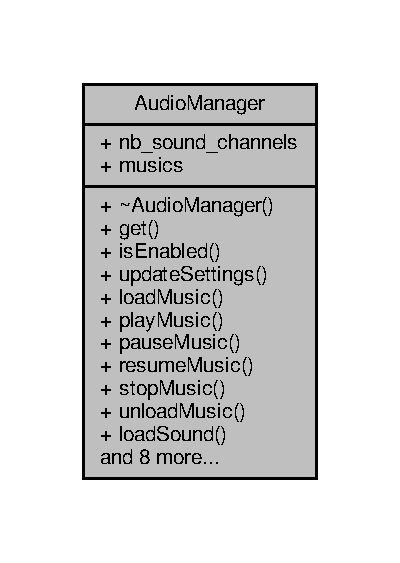
\includegraphics[width=192pt]{class_audio_manager__coll__graph}
\end{center}
\end{figure}
\doxysubsection*{Public Member Functions}
\begin{DoxyCompactItemize}
\item 
\mbox{\Hypertarget{class_audio_manager_ad94dc46723c6d7cf8c81fc3772a842aa}\label{class_audio_manager_ad94dc46723c6d7cf8c81fc3772a842aa}} 
\mbox{\hyperlink{class_audio_manager_ad94dc46723c6d7cf8c81fc3772a842aa}{$\sim$\+Audio\+Manager}} ()
\begin{DoxyCompactList}\small\item\em Destroy the Audio Manager\+:\+: Audio Manager object. \end{DoxyCompactList}\end{DoxyCompactItemize}
\doxysubsection*{Static Public Member Functions}
\begin{DoxyCompactItemize}
\item 
static \mbox{\hyperlink{class_audio_manager}{Audio\+Manager}} \& \mbox{\hyperlink{class_audio_manager_ac8e8acadc8bba682bd3835997d379f5c}{get}} ()
\begin{DoxyCompactList}\small\item\em Return a reference to the singleton \mbox{\hyperlink{class_audio_manager}{Audio\+Manager}}. \end{DoxyCompactList}\item 
static bool \mbox{\hyperlink{class_audio_manager_a68184311194e3f5609e34b8e806655b9}{is\+Enabled}} ()
\begin{DoxyCompactList}\small\item\em Indicate if the \mbox{\hyperlink{class_audio_manager}{Audio\+Manager}} has been correctly initialized. \end{DoxyCompactList}\item 
\mbox{\Hypertarget{class_audio_manager_ad690966e6184debfb05c160d2bbda6a8}\label{class_audio_manager_ad690966e6184debfb05c160d2bbda6a8}} 
static void \mbox{\hyperlink{class_audio_manager_ad690966e6184debfb05c160d2bbda6a8}{update\+Settings}} ()
\begin{DoxyCompactList}\small\item\em Change the volume for the music and all the sound being played. If the music was set with a volume modifier lower than 1.\+0, it will be conserved. \end{DoxyCompactList}\item 
static void \mbox{\hyperlink{class_audio_manager_a3bb15b3e23faa7ddd6ccd39da27d8484}{load\+Music}} (std\+::string file\+\_\+name, bool silent=true)
\begin{DoxyCompactList}\small\item\em Load a new music from its file name. \end{DoxyCompactList}\item 
static void \mbox{\hyperlink{class_audio_manager_ae0f9ebfae17ee406df9f2fb3b7701a4c}{play\+Music}} (std\+::string music\+\_\+name, float volume=1.\+0, bool loop=false)
\begin{DoxyCompactList}\small\item\em Play a music with a volume modifier. \end{DoxyCompactList}\item 
\mbox{\Hypertarget{class_audio_manager_a8afd8f3db6787f87aa55436d6c9dadf1}\label{class_audio_manager_a8afd8f3db6787f87aa55436d6c9dadf1}} 
static void \mbox{\hyperlink{class_audio_manager_a8afd8f3db6787f87aa55436d6c9dadf1}{pause\+Music}} ()
\begin{DoxyCompactList}\small\item\em Pause the music currently played. \end{DoxyCompactList}\item 
\mbox{\Hypertarget{class_audio_manager_a213a73d801ac409765010ba6d7a8f4f3}\label{class_audio_manager_a213a73d801ac409765010ba6d7a8f4f3}} 
static void \mbox{\hyperlink{class_audio_manager_a213a73d801ac409765010ba6d7a8f4f3}{resume\+Music}} ()
\begin{DoxyCompactList}\small\item\em Resume the music currently played. \end{DoxyCompactList}\item 
\mbox{\Hypertarget{class_audio_manager_a72a288a0d8397bed1a9a39efca363326}\label{class_audio_manager_a72a288a0d8397bed1a9a39efca363326}} 
static void \mbox{\hyperlink{class_audio_manager_a72a288a0d8397bed1a9a39efca363326}{stop\+Music}} ()
\begin{DoxyCompactList}\small\item\em Stop the music currently played. \end{DoxyCompactList}\item 
static void \mbox{\hyperlink{class_audio_manager_a6abc50fbd069dae8b38bb8d8aa9476cd}{unload\+Music}} (std\+::string music\+\_\+name)
\begin{DoxyCompactList}\small\item\em Unload the music from the audio manager. \end{DoxyCompactList}\item 
static void \mbox{\hyperlink{class_audio_manager_a6a0b83c130c022c7557bcc4edb7c59d8}{load\+Sound}} (std\+::string file\+\_\+name, bool silent=true)
\begin{DoxyCompactList}\small\item\em Load a new sound from its file name. \end{DoxyCompactList}\item 
static void \mbox{\hyperlink{class_audio_manager_a54e2edf4bdf4702431e7afae0db8955c}{play\+Sound}} (std\+::string sound\+\_\+name, float volume=1.\+0, bool loop=false, bool mute\+Music=false, int fade\+In=0)
\begin{DoxyCompactList}\small\item\em Play a sound identified by file name with a volume modifier. \end{DoxyCompactList}\item 
static void \mbox{\hyperlink{class_audio_manager_ada650abafa8b74a4a0d23cadccee033f}{pause\+Sound}} (std\+::string sound\+\_\+name)
\begin{DoxyCompactList}\small\item\em Pause all the channels of the sound identified by file name. \end{DoxyCompactList}\item 
static void \mbox{\hyperlink{class_audio_manager_acb3fab4f831354f04948f835b8a6c51a}{resume\+Sound}} (std\+::string sound\+\_\+name)
\item 
static void \mbox{\hyperlink{class_audio_manager_a39a5ca72b2201306a7fd1506a3744286}{stop\+Sound}} (std\+::string sound\+\_\+name)
\begin{DoxyCompactList}\small\item\em Stop all the channels of the sound identified by file name. \end{DoxyCompactList}\item 
\mbox{\Hypertarget{class_audio_manager_aa660fe4ee049d2606471d000c96d50a0}\label{class_audio_manager_aa660fe4ee049d2606471d000c96d50a0}} 
static void \mbox{\hyperlink{class_audio_manager_aa660fe4ee049d2606471d000c96d50a0}{pause\+All\+Sounds}} ()
\begin{DoxyCompactList}\small\item\em Pause all the channels. \end{DoxyCompactList}\item 
\mbox{\Hypertarget{class_audio_manager_af7d83968ccbfb2eac4def898630e2624}\label{class_audio_manager_af7d83968ccbfb2eac4def898630e2624}} 
static void \mbox{\hyperlink{class_audio_manager_af7d83968ccbfb2eac4def898630e2624}{resume\+All\+Sounds}} ()
\begin{DoxyCompactList}\small\item\em Resume all the channels. \end{DoxyCompactList}\item 
static void \mbox{\hyperlink{class_audio_manager_af492087dd75a160562ef06c6600f54b5}{unload\+Sound}} (std\+::string sound\+\_\+name)
\begin{DoxyCompactList}\small\item\em Unload the sound identified by file name. \end{DoxyCompactList}\item 
\mbox{\Hypertarget{class_audio_manager_ac880de40f09c0065c10948ca138cc7be}\label{class_audio_manager_ac880de40f09c0065c10948ca138cc7be}} 
static void \mbox{\hyperlink{class_audio_manager_ac880de40f09c0065c10948ca138cc7be}{stop\+All\+Sounds}} ()
\begin{DoxyCompactList}\small\item\em Stop all the channels. \end{DoxyCompactList}\end{DoxyCompactItemize}
\doxysubsection*{Static Public Attributes}
\begin{DoxyCompactItemize}
\item 
static const int \mbox{\hyperlink{class_audio_manager_abd1cfb41f75592fc90007aad609a11ee}{nb\+\_\+sound\+\_\+channels}} = 42
\item 
static std\+::vector$<$ std\+::string $>$ \mbox{\hyperlink{class_audio_manager_ab4f16f2b8df28e812c60769c534644b0}{musics}}
\end{DoxyCompactItemize}


\doxysubsection{Detailed Description}
This is the audio manager. In this static class, you can play musics and sound. 

\doxysubsection{Member Function Documentation}
\mbox{\Hypertarget{class_audio_manager_ac8e8acadc8bba682bd3835997d379f5c}\label{class_audio_manager_ac8e8acadc8bba682bd3835997d379f5c}} 
\index{AudioManager@{AudioManager}!get@{get}}
\index{get@{get}!AudioManager@{AudioManager}}
\doxysubsubsection{\texorpdfstring{get()}{get()}}
{\footnotesize\ttfamily \mbox{\hyperlink{class_audio_manager}{Audio\+Manager}} \& Audio\+Manager\+::get (\begin{DoxyParamCaption}{ }\end{DoxyParamCaption})\hspace{0.3cm}{\ttfamily [static]}}



Return a reference to the singleton \mbox{\hyperlink{class_audio_manager}{Audio\+Manager}}. 

\begin{DoxyReturn}{Returns}
\mbox{\hyperlink{class_audio_manager}{Audio\+Manager}}\& the reference to the singleton. 
\end{DoxyReturn}
\mbox{\Hypertarget{class_audio_manager_a68184311194e3f5609e34b8e806655b9}\label{class_audio_manager_a68184311194e3f5609e34b8e806655b9}} 
\index{AudioManager@{AudioManager}!isEnabled@{isEnabled}}
\index{isEnabled@{isEnabled}!AudioManager@{AudioManager}}
\doxysubsubsection{\texorpdfstring{isEnabled()}{isEnabled()}}
{\footnotesize\ttfamily bool Audio\+Manager\+::is\+Enabled (\begin{DoxyParamCaption}{ }\end{DoxyParamCaption})\hspace{0.3cm}{\ttfamily [static]}}



Indicate if the \mbox{\hyperlink{class_audio_manager}{Audio\+Manager}} has been correctly initialized. 

\begin{DoxyReturn}{Returns}
true if the \mbox{\hyperlink{class_audio_manager}{Audio\+Manager}} is working. 

false otherwise. 
\end{DoxyReturn}
\mbox{\Hypertarget{class_audio_manager_a3bb15b3e23faa7ddd6ccd39da27d8484}\label{class_audio_manager_a3bb15b3e23faa7ddd6ccd39da27d8484}} 
\index{AudioManager@{AudioManager}!loadMusic@{loadMusic}}
\index{loadMusic@{loadMusic}!AudioManager@{AudioManager}}
\doxysubsubsection{\texorpdfstring{loadMusic()}{loadMusic()}}
{\footnotesize\ttfamily void Audio\+Manager\+::load\+Music (\begin{DoxyParamCaption}\item[{std\+::string}]{file\+\_\+name,  }\item[{bool}]{silent = {\ttfamily true} }\end{DoxyParamCaption})\hspace{0.3cm}{\ttfamily [static]}}



Load a new music from its file name. 


\begin{DoxyParams}{Parameters}
{\em file\+\_\+name} & The path to the music file, starting from the asset directory. \\
\hline
{\em silent} & Don\textquotesingle{}t show warning if enabled\\
\hline
\end{DoxyParams}

\begin{DoxyExceptions}{Exceptions}
{\em A} & Music\+Exception if the music failed to be loaded. The path might be incorrect. \\
\hline
\end{DoxyExceptions}
\mbox{\Hypertarget{class_audio_manager_a6a0b83c130c022c7557bcc4edb7c59d8}\label{class_audio_manager_a6a0b83c130c022c7557bcc4edb7c59d8}} 
\index{AudioManager@{AudioManager}!loadSound@{loadSound}}
\index{loadSound@{loadSound}!AudioManager@{AudioManager}}
\doxysubsubsection{\texorpdfstring{loadSound()}{loadSound()}}
{\footnotesize\ttfamily void Audio\+Manager\+::load\+Sound (\begin{DoxyParamCaption}\item[{std\+::string}]{file\+\_\+name,  }\item[{bool}]{silent = {\ttfamily true} }\end{DoxyParamCaption})\hspace{0.3cm}{\ttfamily [static]}}



Load a new sound from its file name. 


\begin{DoxyParams}{Parameters}
{\em file\+\_\+name} & The path to the sound file, starting from the asset directory. \\
\hline
{\em silent} & Don\textquotesingle{}t show warning if enabled\\
\hline
\end{DoxyParams}

\begin{DoxyExceptions}{Exceptions}
{\em A} & Sound\+Exception if the sound failed to be loaded. The path might be incorrect. \\
\hline
\end{DoxyExceptions}
\mbox{\Hypertarget{class_audio_manager_ada650abafa8b74a4a0d23cadccee033f}\label{class_audio_manager_ada650abafa8b74a4a0d23cadccee033f}} 
\index{AudioManager@{AudioManager}!pauseSound@{pauseSound}}
\index{pauseSound@{pauseSound}!AudioManager@{AudioManager}}
\doxysubsubsection{\texorpdfstring{pauseSound()}{pauseSound()}}
{\footnotesize\ttfamily void Audio\+Manager\+::pause\+Sound (\begin{DoxyParamCaption}\item[{std\+::string}]{sound\+\_\+name }\end{DoxyParamCaption})\hspace{0.3cm}{\ttfamily [static]}}



Pause all the channels of the sound identified by file name. 


\begin{DoxyParams}{Parameters}
{\em sound\+\_\+name} & the file name of the sound. \\
\hline
\end{DoxyParams}
\mbox{\Hypertarget{class_audio_manager_ae0f9ebfae17ee406df9f2fb3b7701a4c}\label{class_audio_manager_ae0f9ebfae17ee406df9f2fb3b7701a4c}} 
\index{AudioManager@{AudioManager}!playMusic@{playMusic}}
\index{playMusic@{playMusic}!AudioManager@{AudioManager}}
\doxysubsubsection{\texorpdfstring{playMusic()}{playMusic()}}
{\footnotesize\ttfamily void Audio\+Manager\+::play\+Music (\begin{DoxyParamCaption}\item[{std\+::string}]{music\+\_\+name,  }\item[{float}]{volume = {\ttfamily 1.0},  }\item[{bool}]{loop = {\ttfamily false} }\end{DoxyParamCaption})\hspace{0.3cm}{\ttfamily [static]}}



Play a music with a volume modifier. 


\begin{DoxyParams}{Parameters}
{\em music\+\_\+name} & The name of the file of the music we want to play. \\
\hline
{\em volume} & The volume modifier apply on top of the audio setting. Set to 1.\+0 by default. \\
\hline
{\em loop} & Indicate if the music should loop. false by default.\\
\hline
\end{DoxyParams}

\begin{DoxyExceptions}{Exceptions}
{\em A} & Music\+Exception if the music failed to be played. \\
\hline
\end{DoxyExceptions}
\mbox{\Hypertarget{class_audio_manager_a54e2edf4bdf4702431e7afae0db8955c}\label{class_audio_manager_a54e2edf4bdf4702431e7afae0db8955c}} 
\index{AudioManager@{AudioManager}!playSound@{playSound}}
\index{playSound@{playSound}!AudioManager@{AudioManager}}
\doxysubsubsection{\texorpdfstring{playSound()}{playSound()}}
{\footnotesize\ttfamily void Audio\+Manager\+::play\+Sound (\begin{DoxyParamCaption}\item[{std\+::string}]{sound\+\_\+name,  }\item[{float}]{volume = {\ttfamily 1.0},  }\item[{bool}]{loop = {\ttfamily false},  }\item[{bool}]{mute\+Music = {\ttfamily false},  }\item[{int}]{fade\+In = {\ttfamily 0} }\end{DoxyParamCaption})\hspace{0.3cm}{\ttfamily [static]}}



Play a sound identified by file name with a volume modifier. 


\begin{DoxyParams}{Parameters}
{\em sound\+\_\+name} & the file name of the sound. \\
\hline
{\em volume} & The volume modifier apply on top of the audio setting. Set to 1.\+0 by default. \\
\hline
{\em loop} & If the sound is played on loop. \\
\hline
{\em mute\+Music} & If we need to mute the music during the sound. \\
\hline
{\em fade\+In} & Fade\+In\\
\hline
\end{DoxyParams}

\begin{DoxyExceptions}{Exceptions}
{\em A} & Sound\+Exception if the sound failed to be played. \\
\hline
\end{DoxyExceptions}
\mbox{\Hypertarget{class_audio_manager_acb3fab4f831354f04948f835b8a6c51a}\label{class_audio_manager_acb3fab4f831354f04948f835b8a6c51a}} 
\index{AudioManager@{AudioManager}!resumeSound@{resumeSound}}
\index{resumeSound@{resumeSound}!AudioManager@{AudioManager}}
\doxysubsubsection{\texorpdfstring{resumeSound()}{resumeSound()}}
{\footnotesize\ttfamily void Audio\+Manager\+::resume\+Sound (\begin{DoxyParamCaption}\item[{std\+::string}]{sound\+\_\+name }\end{DoxyParamCaption})\hspace{0.3cm}{\ttfamily [static]}}

Resume all the channels of the sound identified by file name.


\begin{DoxyParams}{Parameters}
{\em sound\+\_\+name} & the file name of the sound. \\
\hline
\end{DoxyParams}
\mbox{\Hypertarget{class_audio_manager_a39a5ca72b2201306a7fd1506a3744286}\label{class_audio_manager_a39a5ca72b2201306a7fd1506a3744286}} 
\index{AudioManager@{AudioManager}!stopSound@{stopSound}}
\index{stopSound@{stopSound}!AudioManager@{AudioManager}}
\doxysubsubsection{\texorpdfstring{stopSound()}{stopSound()}}
{\footnotesize\ttfamily void Audio\+Manager\+::stop\+Sound (\begin{DoxyParamCaption}\item[{std\+::string}]{sound\+\_\+name }\end{DoxyParamCaption})\hspace{0.3cm}{\ttfamily [static]}}



Stop all the channels of the sound identified by file name. 


\begin{DoxyParams}{Parameters}
{\em sound\+\_\+name} & the file name of the sound. \\
\hline
\end{DoxyParams}
\mbox{\Hypertarget{class_audio_manager_a6abc50fbd069dae8b38bb8d8aa9476cd}\label{class_audio_manager_a6abc50fbd069dae8b38bb8d8aa9476cd}} 
\index{AudioManager@{AudioManager}!unloadMusic@{unloadMusic}}
\index{unloadMusic@{unloadMusic}!AudioManager@{AudioManager}}
\doxysubsubsection{\texorpdfstring{unloadMusic()}{unloadMusic()}}
{\footnotesize\ttfamily void Audio\+Manager\+::unload\+Music (\begin{DoxyParamCaption}\item[{std\+::string}]{music\+\_\+name }\end{DoxyParamCaption})\hspace{0.3cm}{\ttfamily [static]}}



Unload the music from the audio manager. 


\begin{DoxyParams}{Parameters}
{\em music\+\_\+name} & The path to the music file, starting from the asset directory. \\
\hline
\end{DoxyParams}
\mbox{\Hypertarget{class_audio_manager_af492087dd75a160562ef06c6600f54b5}\label{class_audio_manager_af492087dd75a160562ef06c6600f54b5}} 
\index{AudioManager@{AudioManager}!unloadSound@{unloadSound}}
\index{unloadSound@{unloadSound}!AudioManager@{AudioManager}}
\doxysubsubsection{\texorpdfstring{unloadSound()}{unloadSound()}}
{\footnotesize\ttfamily void Audio\+Manager\+::unload\+Sound (\begin{DoxyParamCaption}\item[{std\+::string}]{sound\+\_\+name }\end{DoxyParamCaption})\hspace{0.3cm}{\ttfamily [static]}}



Unload the sound identified by file name. 


\begin{DoxyParams}{Parameters}
{\em sound\+\_\+name} & the file name of the sound. \\
\hline
\end{DoxyParams}


\doxysubsection{Member Data Documentation}
\mbox{\Hypertarget{class_audio_manager_ab4f16f2b8df28e812c60769c534644b0}\label{class_audio_manager_ab4f16f2b8df28e812c60769c534644b0}} 
\index{AudioManager@{AudioManager}!musics@{musics}}
\index{musics@{musics}!AudioManager@{AudioManager}}
\doxysubsubsection{\texorpdfstring{musics}{musics}}
{\footnotesize\ttfamily std\+::vector$<$ std\+::string $>$ Audio\+Manager\+::musics\hspace{0.3cm}{\ttfamily [static]}}

{\bfseries Initial value\+:}
\begin{DoxyCode}{0}
\DoxyCodeLine{= \{}
\DoxyCodeLine{    \textcolor{stringliteral}{"sounds/french79-\/between\_the\_buttons.ogg"},}
\DoxyCodeLine{    \textcolor{stringliteral}{"sounds/french79-\/naked\_city.ogg"},}
\DoxyCodeLine{    \textcolor{stringliteral}{"sounds/superpoze-\/siver\_head.ogg"},}
\DoxyCodeLine{    \textcolor{stringliteral}{"sounds/the\_blaze-\/territory.ogg"},}
\DoxyCodeLine{    \textcolor{stringliteral}{"sounds/eirik\_suhrke-\/a\_new\_morning.ogg"},}
\DoxyCodeLine{    \textcolor{stringliteral}{"sounds/moon-\/crystals.ogg"},}
\DoxyCodeLine{    \textcolor{stringliteral}{"sounds/moon-\/hydrogen.ogg"}}
\DoxyCodeLine{\}}

\end{DoxyCode}
Al musics \mbox{\Hypertarget{class_audio_manager_abd1cfb41f75592fc90007aad609a11ee}\label{class_audio_manager_abd1cfb41f75592fc90007aad609a11ee}} 
\index{AudioManager@{AudioManager}!nb\_sound\_channels@{nb\_sound\_channels}}
\index{nb\_sound\_channels@{nb\_sound\_channels}!AudioManager@{AudioManager}}
\doxysubsubsection{\texorpdfstring{nb\_sound\_channels}{nb\_sound\_channels}}
{\footnotesize\ttfamily const int Audio\+Manager\+::nb\+\_\+sound\+\_\+channels = 42\hspace{0.3cm}{\ttfamily [static]}}

Number of sounds channel 

The documentation for this class was generated from the following files\+:\begin{DoxyCompactItemize}
\item 
includes/audio/Audio\+Manager.\+hpp\item 
srcs/audio/Audio\+Manager.\+cpp\end{DoxyCompactItemize}

\hypertarget{class_bomb}{}\doxysection{Bomb Class Reference}
\label{class_bomb}\index{Bomb@{Bomb}}


This is the bomb object.  




{\ttfamily \#include $<$Bomb.\+hpp$>$}



Inheritance diagram for Bomb\+:\nopagebreak
\begin{figure}[H]
\begin{center}
\leavevmode
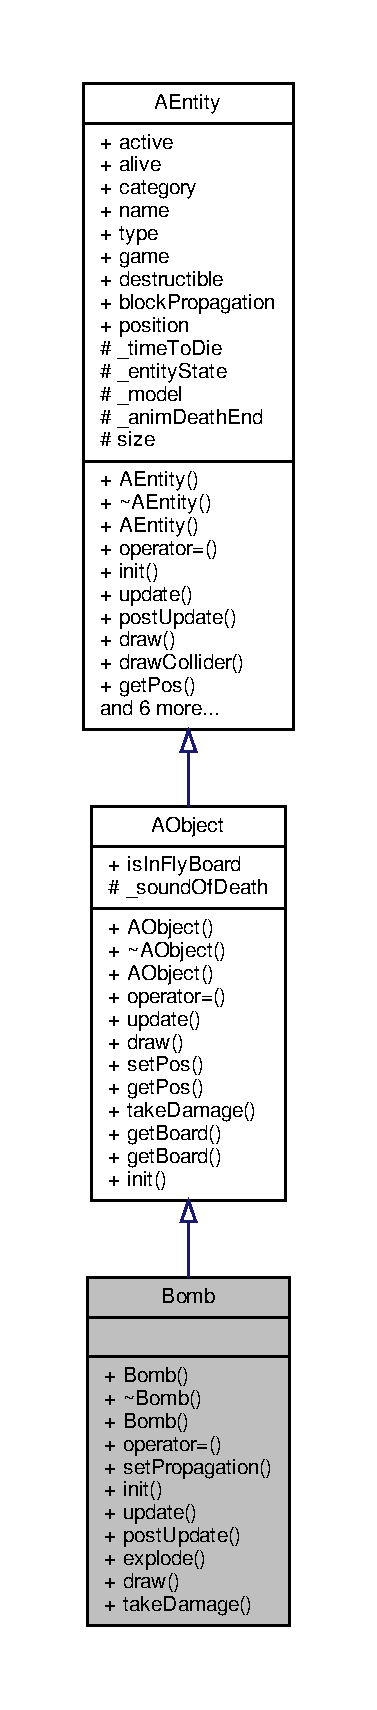
\includegraphics[height=550pt]{class_bomb__inherit__graph}
\end{center}
\end{figure}


Collaboration diagram for Bomb\+:
\nopagebreak
\begin{figure}[H]
\begin{center}
\leavevmode
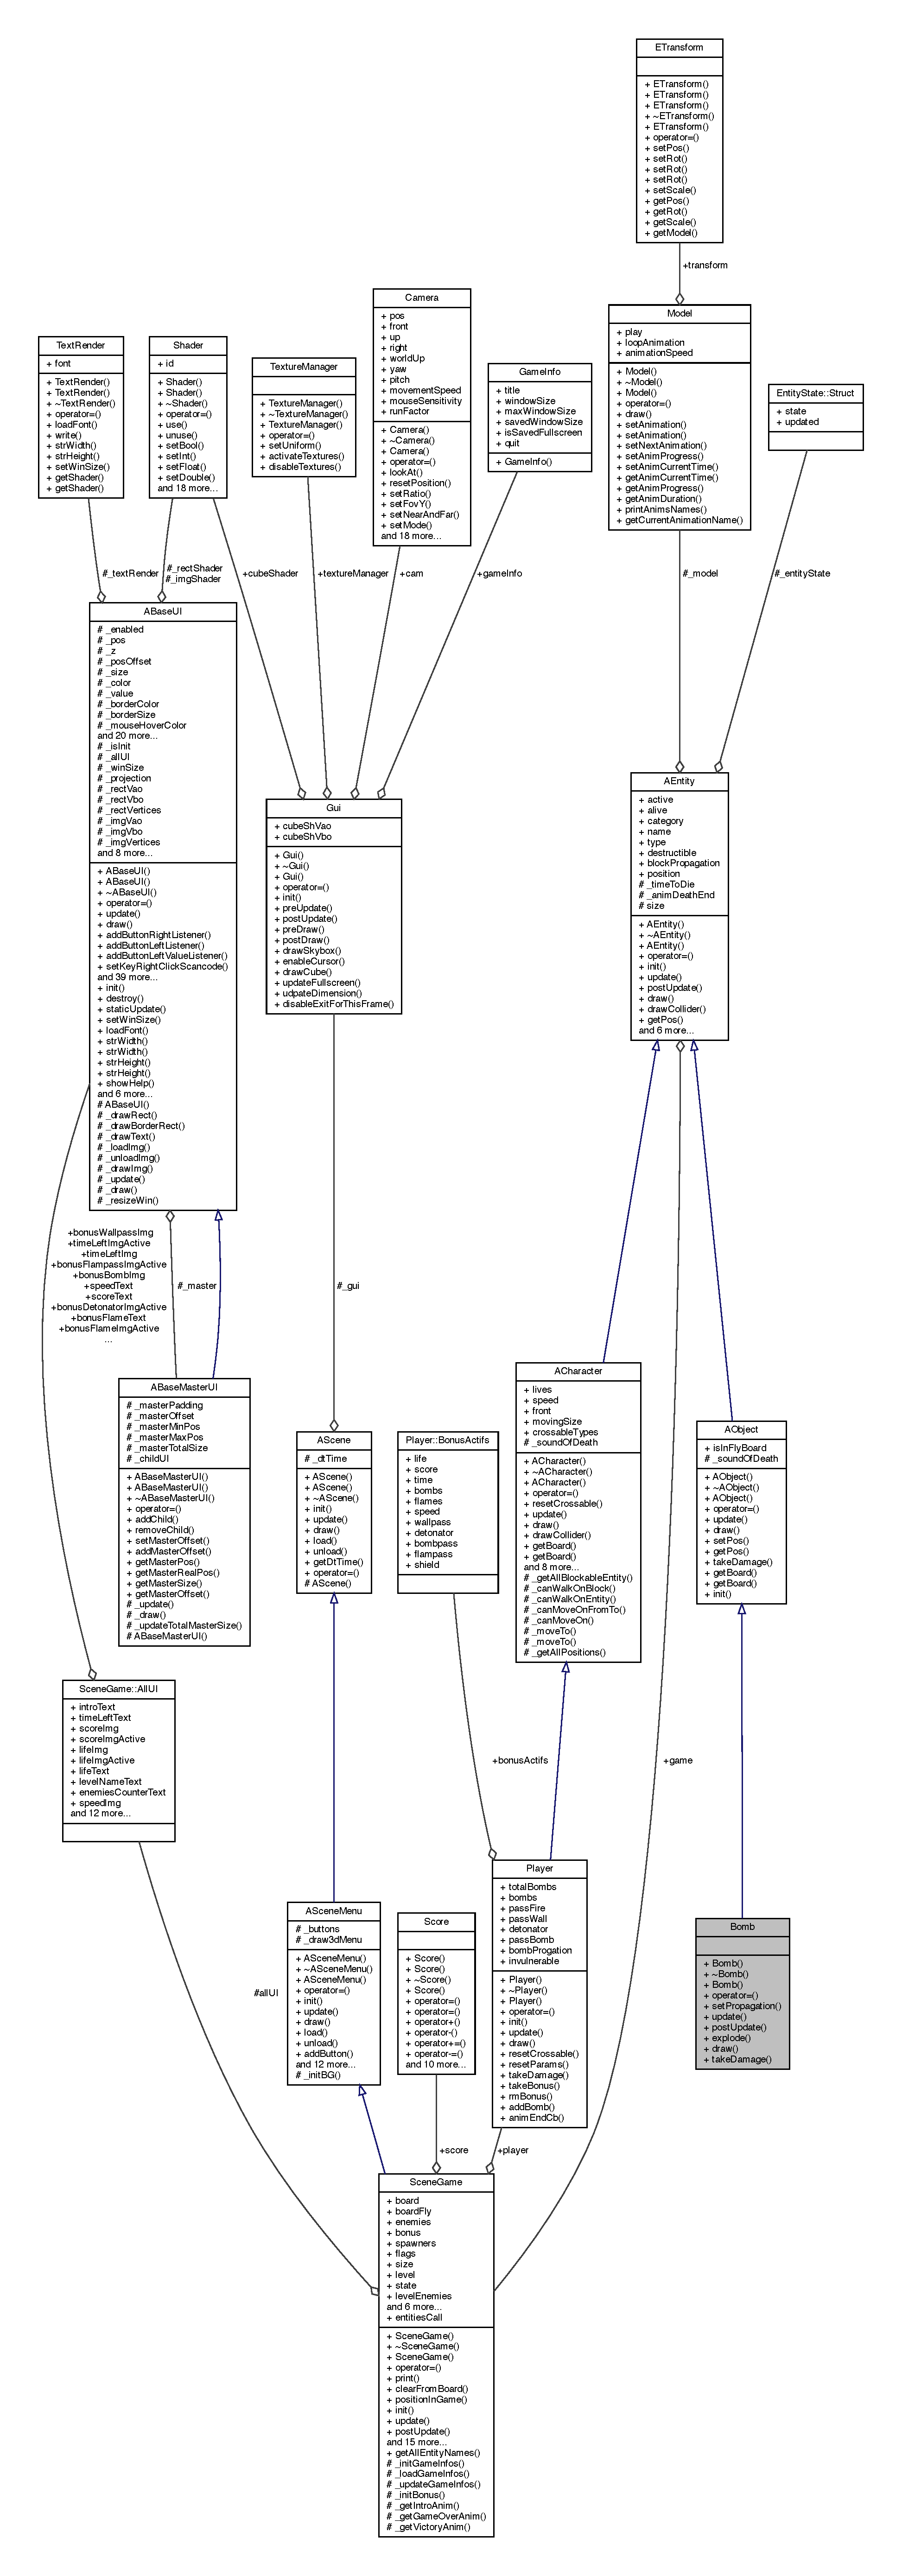
\includegraphics[height=550pt]{class_bomb__coll__graph}
\end{center}
\end{figure}
\doxysubsection*{Classes}
\begin{DoxyCompactItemize}
\item 
class \mbox{\hyperlink{class_bomb_1_1_bomb_exception}{Bomb\+Exception}}
\begin{DoxyCompactList}\small\item\em \mbox{\hyperlink{class_bomb}{Bomb}} exception. \end{DoxyCompactList}\end{DoxyCompactItemize}
\doxysubsection*{Public Member Functions}
\begin{DoxyCompactItemize}
\item 
\mbox{\hyperlink{class_bomb_aa09b8879ab7aae611b05ad0e73e45696}{Bomb}} (\mbox{\hyperlink{class_scene_game}{Scene\+Game}} \&\mbox{\hyperlink{class_a_entity_aa2c05db944a8b7487eb8470dd20211ab}{game}})
\begin{DoxyCompactList}\small\item\em Construct a new \mbox{\hyperlink{class_bomb}{Bomb}}\+:\+: \mbox{\hyperlink{class_bomb}{Bomb}} object. \end{DoxyCompactList}\item 
\mbox{\Hypertarget{class_bomb_acbb47327cfb2fa429887774ef3597965}\label{class_bomb_acbb47327cfb2fa429887774ef3597965}} 
\mbox{\hyperlink{class_bomb_acbb47327cfb2fa429887774ef3597965}{$\sim$\+Bomb}} ()
\begin{DoxyCompactList}\small\item\em Destroy the \mbox{\hyperlink{class_bomb}{Bomb}}\+:\+: \mbox{\hyperlink{class_bomb}{Bomb}} object. \end{DoxyCompactList}\item 
\mbox{\hyperlink{class_bomb_ad02ddab443979d610ea5ad04343bd7fa}{Bomb}} (\mbox{\hyperlink{class_bomb}{Bomb}} const \&src)
\begin{DoxyCompactList}\small\item\em Construct a new \mbox{\hyperlink{class_bomb}{Bomb}}\+:\+: \mbox{\hyperlink{class_bomb}{Bomb}} object. \end{DoxyCompactList}\item 
\mbox{\hyperlink{class_bomb}{Bomb}} \& \mbox{\hyperlink{class_bomb_a85eb751af149c92278eafdbabced0d3d}{operator=}} (\mbox{\hyperlink{class_bomb}{Bomb}} const \&rhs)
\begin{DoxyCompactList}\small\item\em Copy this object. \end{DoxyCompactList}\item 
\mbox{\hyperlink{class_bomb}{Bomb}} $\ast$ \mbox{\hyperlink{class_bomb_a3a3488cb6bd66f3b6d73003814dfb209}{set\+Propagation}} (const int propagation)
\begin{DoxyCompactList}\small\item\em Set the bomb propagation. \end{DoxyCompactList}\item 
bool \mbox{\hyperlink{class_bomb_a4a3f751937f59953f4cf585b07c9684c}{init}} ()
\begin{DoxyCompactList}\small\item\em Init \mbox{\hyperlink{class_bomb}{Bomb}}. \end{DoxyCompactList}\item 
bool \mbox{\hyperlink{class_bomb_a9808d8efcc57b9ce7b0bd48d95875aad}{update}} ()
\begin{DoxyCompactList}\small\item\em update is called each frame. \end{DoxyCompactList}\item 
bool \mbox{\hyperlink{class_bomb_a443c5d40a92e67ef456c71369e8a111b}{post\+Update}} ()
\begin{DoxyCompactList}\small\item\em Post\+Update is called each frame, after \mbox{\hyperlink{class_bomb_a9808d8efcc57b9ce7b0bd48d95875aad}{update()}}. \end{DoxyCompactList}\item 
void \mbox{\hyperlink{class_bomb_a4d3105c3390626d385bdb5dfd0fa68ff}{explode}} (glm\+::vec2 const pos)
\begin{DoxyCompactList}\small\item\em The bomb explode in the N.\+E.\+S.\+W. directions at \+\_\+propagation distance. \end{DoxyCompactList}\item 
bool \mbox{\hyperlink{class_bomb_ae0ea4aa0ce14d353ad63c31cccc2a69d}{draw}} (\mbox{\hyperlink{class_gui}{Gui}} \&gui)
\begin{DoxyCompactList}\small\item\em draw is called each frame. \end{DoxyCompactList}\item 
bool \mbox{\hyperlink{class_bomb_ac51b260cdfef0cde903a88003994276e}{take\+Damage}} (const int damage)
\begin{DoxyCompactList}\small\item\em Take\+Damage make explode the bomb. \end{DoxyCompactList}\end{DoxyCompactItemize}
\doxysubsection*{Additional Inherited Members}


\doxysubsection{Detailed Description}
This is the bomb object. 

\doxysubsection{Constructor \& Destructor Documentation}
\mbox{\Hypertarget{class_bomb_aa09b8879ab7aae611b05ad0e73e45696}\label{class_bomb_aa09b8879ab7aae611b05ad0e73e45696}} 
\index{Bomb@{Bomb}!Bomb@{Bomb}}
\index{Bomb@{Bomb}!Bomb@{Bomb}}
\doxysubsubsection{\texorpdfstring{Bomb()}{Bomb()}\hspace{0.1cm}{\footnotesize\ttfamily [1/2]}}
{\footnotesize\ttfamily Bomb\+::\+Bomb (\begin{DoxyParamCaption}\item[{\mbox{\hyperlink{class_scene_game}{Scene\+Game}} \&}]{game }\end{DoxyParamCaption})\hspace{0.3cm}{\ttfamily [explicit]}}



Construct a new \mbox{\hyperlink{class_bomb}{Bomb}}\+:\+: \mbox{\hyperlink{class_bomb}{Bomb}} object. 


\begin{DoxyParams}{Parameters}
{\em game} & A reference to the \mbox{\hyperlink{class_scene_game}{Scene\+Game}} master object \\
\hline
\end{DoxyParams}
\mbox{\Hypertarget{class_bomb_ad02ddab443979d610ea5ad04343bd7fa}\label{class_bomb_ad02ddab443979d610ea5ad04343bd7fa}} 
\index{Bomb@{Bomb}!Bomb@{Bomb}}
\index{Bomb@{Bomb}!Bomb@{Bomb}}
\doxysubsubsection{\texorpdfstring{Bomb()}{Bomb()}\hspace{0.1cm}{\footnotesize\ttfamily [2/2]}}
{\footnotesize\ttfamily Bomb\+::\+Bomb (\begin{DoxyParamCaption}\item[{\mbox{\hyperlink{class_bomb}{Bomb}} const \&}]{src }\end{DoxyParamCaption})}



Construct a new \mbox{\hyperlink{class_bomb}{Bomb}}\+:\+: \mbox{\hyperlink{class_bomb}{Bomb}} object. 


\begin{DoxyParams}{Parameters}
{\em src} & The object to do the copy \\
\hline
\end{DoxyParams}


\doxysubsection{Member Function Documentation}
\mbox{\Hypertarget{class_bomb_ae0ea4aa0ce14d353ad63c31cccc2a69d}\label{class_bomb_ae0ea4aa0ce14d353ad63c31cccc2a69d}} 
\index{Bomb@{Bomb}!draw@{draw}}
\index{draw@{draw}!Bomb@{Bomb}}
\doxysubsubsection{\texorpdfstring{draw()}{draw()}}
{\footnotesize\ttfamily bool Bomb\+::draw (\begin{DoxyParamCaption}\item[{\mbox{\hyperlink{class_gui}{Gui}} \&}]{gui }\end{DoxyParamCaption})\hspace{0.3cm}{\ttfamily [virtual]}}



draw is called each frame. 

\begin{DoxyReturn}{Returns}
true if success 

false if failure 
\end{DoxyReturn}


Implements \mbox{\hyperlink{class_a_object_a5e454e13e04ee937c20a465244cf748a}{A\+Object}}.

\mbox{\Hypertarget{class_bomb_a4d3105c3390626d385bdb5dfd0fa68ff}\label{class_bomb_a4d3105c3390626d385bdb5dfd0fa68ff}} 
\index{Bomb@{Bomb}!explode@{explode}}
\index{explode@{explode}!Bomb@{Bomb}}
\doxysubsubsection{\texorpdfstring{explode()}{explode()}}
{\footnotesize\ttfamily void Bomb\+::explode (\begin{DoxyParamCaption}\item[{glm\+::vec2 const}]{pos }\end{DoxyParamCaption})}



The bomb explode in the N.\+E.\+S.\+W. directions at \+\_\+propagation distance. 


\begin{DoxyParams}{Parameters}
{\em pos} & \\
\hline
\end{DoxyParams}
\mbox{\Hypertarget{class_bomb_a4a3f751937f59953f4cf585b07c9684c}\label{class_bomb_a4a3f751937f59953f4cf585b07c9684c}} 
\index{Bomb@{Bomb}!init@{init}}
\index{init@{init}!Bomb@{Bomb}}
\doxysubsubsection{\texorpdfstring{init()}{init()}}
{\footnotesize\ttfamily bool Bomb\+::init (\begin{DoxyParamCaption}{ }\end{DoxyParamCaption})\hspace{0.3cm}{\ttfamily [virtual]}}



Init \mbox{\hyperlink{class_bomb}{Bomb}}. 

\begin{DoxyReturn}{Returns}
true on success 

false on failure 
\end{DoxyReturn}


Reimplemented from \mbox{\hyperlink{class_a_object_afa83ef1c900a47453524219788327b86}{A\+Object}}.

\mbox{\Hypertarget{class_bomb_a85eb751af149c92278eafdbabced0d3d}\label{class_bomb_a85eb751af149c92278eafdbabced0d3d}} 
\index{Bomb@{Bomb}!operator=@{operator=}}
\index{operator=@{operator=}!Bomb@{Bomb}}
\doxysubsubsection{\texorpdfstring{operator=()}{operator=()}}
{\footnotesize\ttfamily \mbox{\hyperlink{class_bomb}{Bomb}} \& Bomb\+::operator= (\begin{DoxyParamCaption}\item[{\mbox{\hyperlink{class_bomb}{Bomb}} const \&}]{rhs }\end{DoxyParamCaption})}



Copy this object. 


\begin{DoxyParams}{Parameters}
{\em rhs} & The object to copy \\
\hline
\end{DoxyParams}
\begin{DoxyReturn}{Returns}
\mbox{\hyperlink{class_bomb}{Bomb}}\& A reference to the copied object 
\end{DoxyReturn}
\mbox{\Hypertarget{class_bomb_a443c5d40a92e67ef456c71369e8a111b}\label{class_bomb_a443c5d40a92e67ef456c71369e8a111b}} 
\index{Bomb@{Bomb}!postUpdate@{postUpdate}}
\index{postUpdate@{postUpdate}!Bomb@{Bomb}}
\doxysubsubsection{\texorpdfstring{postUpdate()}{postUpdate()}}
{\footnotesize\ttfamily bool Bomb\+::post\+Update (\begin{DoxyParamCaption}{ }\end{DoxyParamCaption})\hspace{0.3cm}{\ttfamily [virtual]}}



Post\+Update is called each frame, after \mbox{\hyperlink{class_bomb_a9808d8efcc57b9ce7b0bd48d95875aad}{update()}}. 

\begin{DoxyReturn}{Returns}
true if success 

false if failure 
\end{DoxyReturn}


Reimplemented from \mbox{\hyperlink{class_a_entity_ae2faa1d11e21033a223fef2bc03b9338}{A\+Entity}}.

\mbox{\Hypertarget{class_bomb_a3a3488cb6bd66f3b6d73003814dfb209}\label{class_bomb_a3a3488cb6bd66f3b6d73003814dfb209}} 
\index{Bomb@{Bomb}!setPropagation@{setPropagation}}
\index{setPropagation@{setPropagation}!Bomb@{Bomb}}
\doxysubsubsection{\texorpdfstring{setPropagation()}{setPropagation()}}
{\footnotesize\ttfamily \mbox{\hyperlink{class_bomb}{Bomb}} $\ast$ Bomb\+::set\+Propagation (\begin{DoxyParamCaption}\item[{const int}]{propagation }\end{DoxyParamCaption})}



Set the bomb propagation. 


\begin{DoxyParams}{Parameters}
{\em propagation} & The new propagation \\
\hline
\end{DoxyParams}
\begin{DoxyReturn}{Returns}
Bomb$\ast$ A pointer on this object 
\end{DoxyReturn}
\mbox{\Hypertarget{class_bomb_ac51b260cdfef0cde903a88003994276e}\label{class_bomb_ac51b260cdfef0cde903a88003994276e}} 
\index{Bomb@{Bomb}!takeDamage@{takeDamage}}
\index{takeDamage@{takeDamage}!Bomb@{Bomb}}
\doxysubsubsection{\texorpdfstring{takeDamage()}{takeDamage()}}
{\footnotesize\ttfamily bool Bomb\+::take\+Damage (\begin{DoxyParamCaption}\item[{const int}]{damage }\end{DoxyParamCaption})\hspace{0.3cm}{\ttfamily [virtual]}}



Take\+Damage make explode the bomb. 


\begin{DoxyParams}{Parameters}
{\em damage} & \\
\hline
\end{DoxyParams}
\begin{DoxyReturn}{Returns}
true if damage taken 

false if damage not taken 
\end{DoxyReturn}


Reimplemented from \mbox{\hyperlink{class_a_object_a39b1720ae5a820512ab4db0906f03b15}{A\+Object}}.

\mbox{\Hypertarget{class_bomb_a9808d8efcc57b9ce7b0bd48d95875aad}\label{class_bomb_a9808d8efcc57b9ce7b0bd48d95875aad}} 
\index{Bomb@{Bomb}!update@{update}}
\index{update@{update}!Bomb@{Bomb}}
\doxysubsubsection{\texorpdfstring{update()}{update()}}
{\footnotesize\ttfamily bool Bomb\+::update (\begin{DoxyParamCaption}{ }\end{DoxyParamCaption})\hspace{0.3cm}{\ttfamily [virtual]}}



update is called each frame. 

\begin{DoxyReturn}{Returns}
true if success 

false if failure 
\end{DoxyReturn}


Implements \mbox{\hyperlink{class_a_object_af35bb4b68af0a11bb1fcf617bde41ecd}{A\+Object}}.



The documentation for this class was generated from the following files\+:\begin{DoxyCompactItemize}
\item 
includes/elements/Bomb.\+hpp\item 
srcs/elements/Bomb.\+cpp\end{DoxyCompactItemize}

\hypertarget{class_bomb_1_1_bomb_exception}{}\doxysection{Bomb\+::Bomb\+Exception Class Reference}
\label{class_bomb_1_1_bomb_exception}\index{Bomb::BombException@{Bomb::BombException}}
Inheritance diagram for Bomb\+::Bomb\+Exception\+:\begin{figure}[H]
\begin{center}
\leavevmode
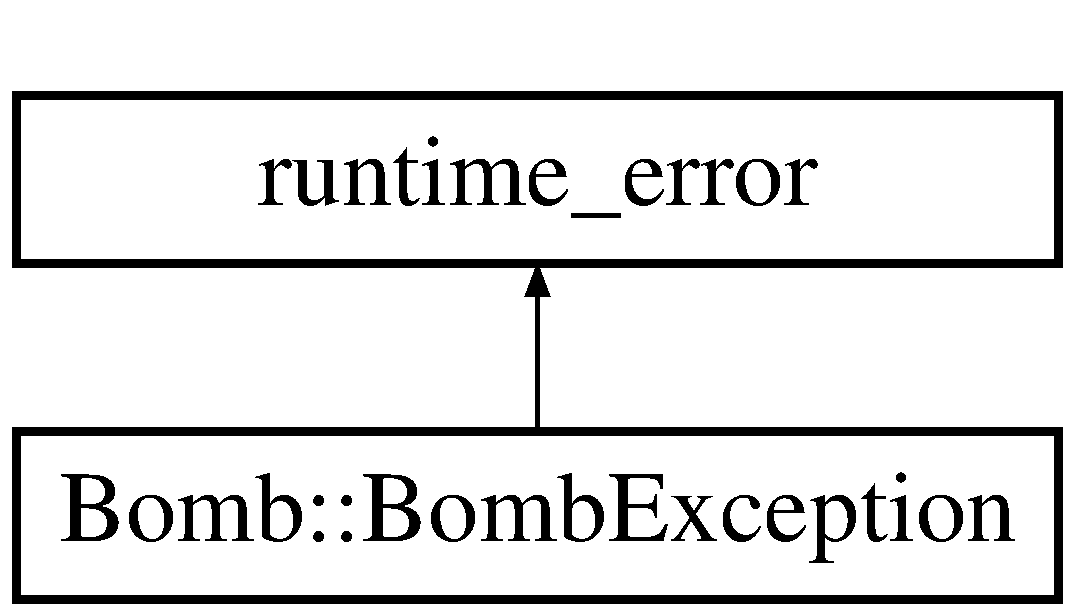
\includegraphics[height=2.000000cm]{class_bomb_1_1_bomb_exception}
\end{center}
\end{figure}
\doxysubsection*{Public Member Functions}
\begin{DoxyCompactItemize}
\item 
\mbox{\Hypertarget{class_bomb_1_1_bomb_exception_abfc03144ee516faa4f3ac4b82f3ccd42}\label{class_bomb_1_1_bomb_exception_abfc03144ee516faa4f3ac4b82f3ccd42}} 
{\bfseries Bomb\+Exception} (const char $\ast$what\+\_\+arg)
\end{DoxyCompactItemize}


The documentation for this class was generated from the following files\+:\begin{DoxyCompactItemize}
\item 
includes/Bomb.\+hpp\item 
srcs/Bomb.\+cpp\end{DoxyCompactItemize}

\hypertarget{class_bonus}{}\doxysection{Bonus Class Reference}
\label{class_bonus}\index{Bonus@{Bonus}}


Inheritance diagram for Bonus\+:\nopagebreak
\begin{figure}[H]
\begin{center}
\leavevmode
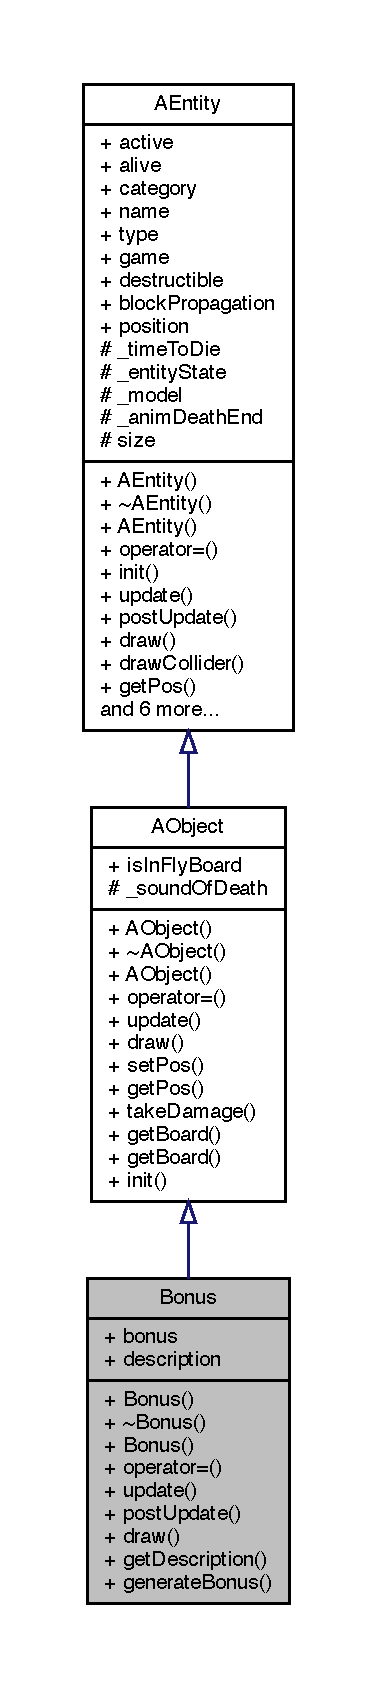
\includegraphics[height=550pt]{class_bonus__inherit__graph}
\end{center}
\end{figure}


Collaboration diagram for Bonus\+:\nopagebreak
\begin{figure}[H]
\begin{center}
\leavevmode
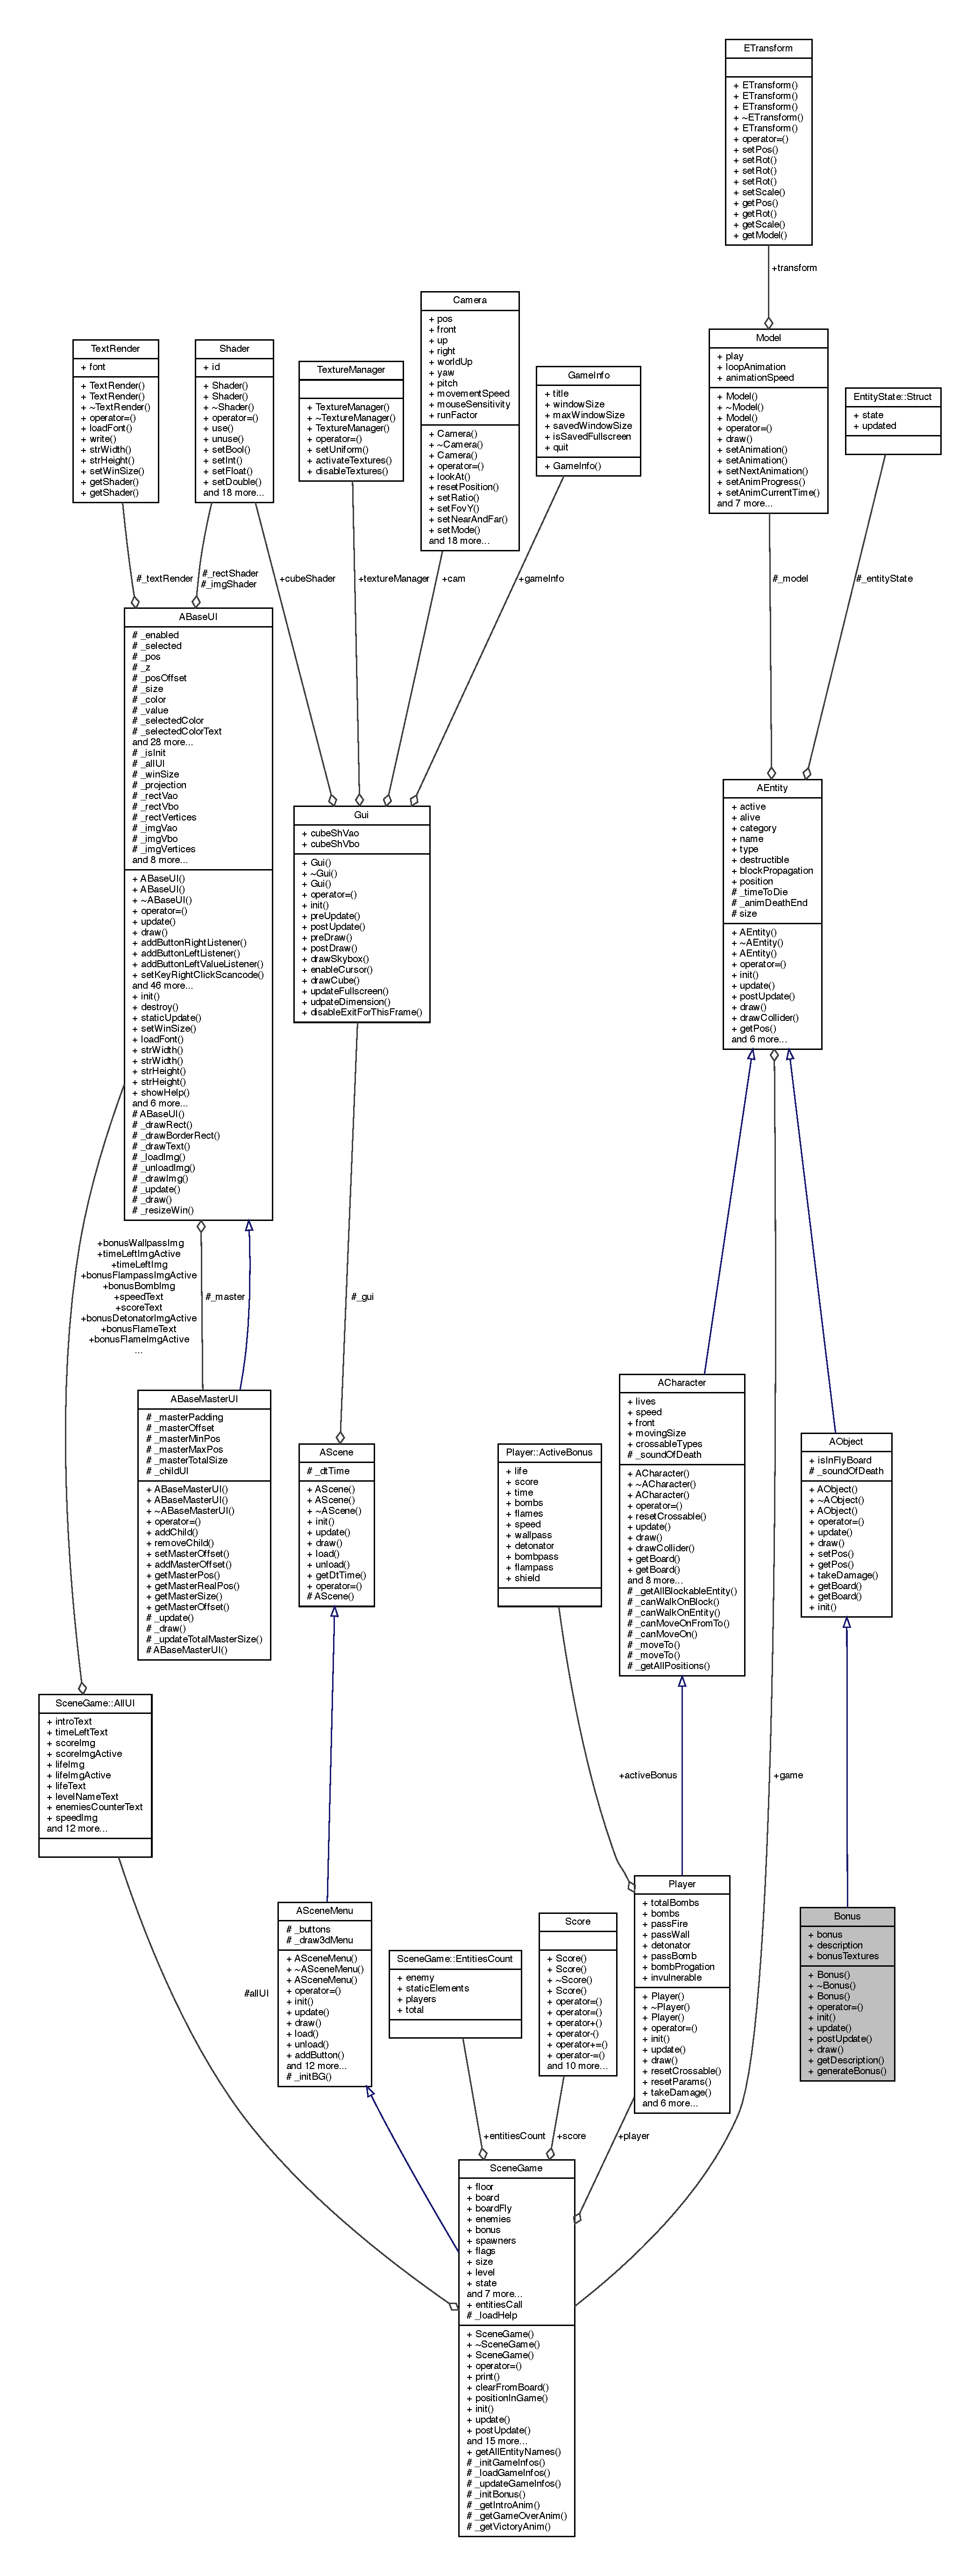
\includegraphics[height=550pt]{class_bonus__coll__graph}
\end{center}
\end{figure}
\doxysubsection*{Classes}
\begin{DoxyCompactItemize}
\item 
class \mbox{\hyperlink{class_bonus_1_1_bonus_exception}{Bonus\+Exception}}
\end{DoxyCompactItemize}
\doxysubsection*{Public Member Functions}
\begin{DoxyCompactItemize}
\item 
\mbox{\Hypertarget{class_bonus_a35c21e394ed7467d9bf1038cffc77047}\label{class_bonus_a35c21e394ed7467d9bf1038cffc77047}} 
{\bfseries Bonus} (\mbox{\hyperlink{class_scene_game}{Scene\+Game}} \&\mbox{\hyperlink{class_a_entity_aa2c05db944a8b7487eb8470dd20211ab}{game}})
\item 
\mbox{\Hypertarget{class_bonus_aedadb1a74a12d5c42f7dc26db1823ebd}\label{class_bonus_aedadb1a74a12d5c42f7dc26db1823ebd}} 
{\bfseries Bonus} (\mbox{\hyperlink{class_bonus}{Bonus}} const \&src)
\item 
\mbox{\Hypertarget{class_bonus_a739b5ec5b1e7214fd0398e4a7970529e}\label{class_bonus_a739b5ec5b1e7214fd0398e4a7970529e}} 
\mbox{\hyperlink{class_bonus}{Bonus}} \& {\bfseries operator=} (\mbox{\hyperlink{class_bonus}{Bonus}} const \&rhs)
\item 
bool \mbox{\hyperlink{class_bonus_a0dd8aa4474c3d1ef494ed8a916cc16cd}{update}} ()
\begin{DoxyCompactList}\small\item\em update is called each frame. \end{DoxyCompactList}\item 
bool \mbox{\hyperlink{class_bonus_a6524cf732f98dfc3baa7f41bbdf13b11}{post\+Update}} ()
\begin{DoxyCompactList}\small\item\em post\+Update is called each frame. After \mbox{\hyperlink{class_bonus_a0dd8aa4474c3d1ef494ed8a916cc16cd}{update()}} \end{DoxyCompactList}\item 
bool \mbox{\hyperlink{class_bonus_acdb40deca7be37984084fb3d4fef85ed}{draw}} (\mbox{\hyperlink{class_gui}{Gui}} \&gui)
\begin{DoxyCompactList}\small\item\em draw is called each frame. \end{DoxyCompactList}\end{DoxyCompactItemize}
\doxysubsection*{Static Public Member Functions}
\begin{DoxyCompactItemize}
\item 
static std\+::string \mbox{\hyperlink{class_bonus_a1d044965859366e57fbe7fcb1eb8a458}{get\+Description}} (Bonus\+Type\+::\+Enum \mbox{\hyperlink{class_a_entity_a4cddb4c9fbae86691e73940edc3731c3}{type}})
\begin{DoxyCompactList}\small\item\em Get the description of a given bonus. \end{DoxyCompactList}\item 
static \mbox{\hyperlink{class_bonus}{Bonus}} $\ast$ \mbox{\hyperlink{class_bonus_a69c5cd0fdef8eef925b5d295696b19a9}{generate\+Bonus}} (\mbox{\hyperlink{class_scene_game}{Scene\+Game}} \&\mbox{\hyperlink{class_a_entity_aa2c05db944a8b7487eb8470dd20211ab}{game}}, float rate=0.\+1f)
\begin{DoxyCompactList}\small\item\em Static class to generate bonus. \end{DoxyCompactList}\end{DoxyCompactItemize}
\doxysubsection*{Static Public Attributes}
\begin{DoxyCompactItemize}
\item 
static std\+::unordered\+\_\+map$<$ std\+::string, Bonus\+Type\+::\+Enum $>$ {\bfseries bonus}
\item 
static std\+::map$<$ Bonus\+Type\+::\+Enum, std\+::string $>$ {\bfseries description}
\end{DoxyCompactItemize}
\doxysubsection*{Additional Inherited Members}


\doxysubsection{Member Function Documentation}
\mbox{\Hypertarget{class_bonus_acdb40deca7be37984084fb3d4fef85ed}\label{class_bonus_acdb40deca7be37984084fb3d4fef85ed}} 
\index{Bonus@{Bonus}!draw@{draw}}
\index{draw@{draw}!Bonus@{Bonus}}
\doxysubsubsection{\texorpdfstring{draw()}{draw()}}
{\footnotesize\ttfamily bool Bonus\+::draw (\begin{DoxyParamCaption}\item[{\mbox{\hyperlink{class_gui}{Gui}} \&}]{gui }\end{DoxyParamCaption})\hspace{0.3cm}{\ttfamily [virtual]}}



draw is called each frame. 

\begin{DoxyReturn}{Returns}
true if success 

false if failure 
\end{DoxyReturn}


Implements \mbox{\hyperlink{class_a_object}{A\+Object}}.

\mbox{\Hypertarget{class_bonus_a69c5cd0fdef8eef925b5d295696b19a9}\label{class_bonus_a69c5cd0fdef8eef925b5d295696b19a9}} 
\index{Bonus@{Bonus}!generateBonus@{generateBonus}}
\index{generateBonus@{generateBonus}!Bonus@{Bonus}}
\doxysubsubsection{\texorpdfstring{generateBonus()}{generateBonus()}}
{\footnotesize\ttfamily \mbox{\hyperlink{class_bonus}{Bonus}} $\ast$ Bonus\+::generate\+Bonus (\begin{DoxyParamCaption}\item[{\mbox{\hyperlink{class_scene_game}{Scene\+Game}} \&}]{game,  }\item[{float}]{rate = {\ttfamily 0.1f} }\end{DoxyParamCaption})\hspace{0.3cm}{\ttfamily [static]}}



Static class to generate bonus. 


\begin{DoxyParams}{Parameters}
{\em game} & \mbox{\hyperlink{class_scene_game}{Scene\+Game}} object. \\
\hline
{\em rate} & Probability to generate an bonus (between 0 and 1). default\+: 0.\+1f \\
\hline
\end{DoxyParams}
\begin{DoxyReturn}{Returns}
Bonus$\ast$ or nullptr if nothing has been generated. 
\end{DoxyReturn}
\mbox{\Hypertarget{class_bonus_a1d044965859366e57fbe7fcb1eb8a458}\label{class_bonus_a1d044965859366e57fbe7fcb1eb8a458}} 
\index{Bonus@{Bonus}!getDescription@{getDescription}}
\index{getDescription@{getDescription}!Bonus@{Bonus}}
\doxysubsubsection{\texorpdfstring{getDescription()}{getDescription()}}
{\footnotesize\ttfamily std\+::string Bonus\+::get\+Description (\begin{DoxyParamCaption}\item[{Bonus\+Type\+::\+Enum}]{type }\end{DoxyParamCaption})\hspace{0.3cm}{\ttfamily [static]}}



Get the description of a given bonus. 


\begin{DoxyParams}{Parameters}
{\em type} & The bonus type \\
\hline
\end{DoxyParams}
\begin{DoxyReturn}{Returns}
std\+::string The description 
\end{DoxyReturn}
\mbox{\Hypertarget{class_bonus_a6524cf732f98dfc3baa7f41bbdf13b11}\label{class_bonus_a6524cf732f98dfc3baa7f41bbdf13b11}} 
\index{Bonus@{Bonus}!postUpdate@{postUpdate}}
\index{postUpdate@{postUpdate}!Bonus@{Bonus}}
\doxysubsubsection{\texorpdfstring{postUpdate()}{postUpdate()}}
{\footnotesize\ttfamily bool Bonus\+::post\+Update (\begin{DoxyParamCaption}{ }\end{DoxyParamCaption})\hspace{0.3cm}{\ttfamily [virtual]}}



post\+Update is called each frame. After \mbox{\hyperlink{class_bonus_a0dd8aa4474c3d1ef494ed8a916cc16cd}{update()}} 

\begin{DoxyReturn}{Returns}
true if success 

false if failure 
\end{DoxyReturn}


Reimplemented from \mbox{\hyperlink{class_a_entity_ae2faa1d11e21033a223fef2bc03b9338}{A\+Entity}}.

\mbox{\Hypertarget{class_bonus_a0dd8aa4474c3d1ef494ed8a916cc16cd}\label{class_bonus_a0dd8aa4474c3d1ef494ed8a916cc16cd}} 
\index{Bonus@{Bonus}!update@{update}}
\index{update@{update}!Bonus@{Bonus}}
\doxysubsubsection{\texorpdfstring{update()}{update()}}
{\footnotesize\ttfamily bool Bonus\+::update (\begin{DoxyParamCaption}{ }\end{DoxyParamCaption})\hspace{0.3cm}{\ttfamily [virtual]}}



update is called each frame. 

\begin{DoxyReturn}{Returns}
true if success 

false if failure 
\end{DoxyReturn}


Implements \mbox{\hyperlink{class_a_object}{A\+Object}}.



\doxysubsection{Member Data Documentation}
\mbox{\Hypertarget{class_bonus_a6738b5cd2f41a4174a721bc51f495ea9}\label{class_bonus_a6738b5cd2f41a4174a721bc51f495ea9}} 
\index{Bonus@{Bonus}!bonus@{bonus}}
\index{bonus@{bonus}!Bonus@{Bonus}}
\doxysubsubsection{\texorpdfstring{bonus}{bonus}}
{\footnotesize\ttfamily std\+::unordered\+\_\+map$<$ std\+::string, Bonus\+Type\+::\+Enum $>$ Bonus\+::bonus\hspace{0.3cm}{\ttfamily [static]}}

{\bfseries Initial value\+:}
\begin{DoxyCode}{0}
\DoxyCodeLine{= \{}
\DoxyCodeLine{    \{ \textcolor{stringliteral}{"life"}, BonusType::LIFE \},}
\DoxyCodeLine{    \{ \textcolor{stringliteral}{"bombs"}, BonusType::BOMBS \},}
\DoxyCodeLine{    \{ \textcolor{stringliteral}{"flames"}, BonusType::FLAMES \},}
\DoxyCodeLine{    \{ \textcolor{stringliteral}{"speed"}, BonusType::SPEED \},}
\DoxyCodeLine{    \{ \textcolor{stringliteral}{"wallpass"}, BonusType::WALLPASS \},}
\DoxyCodeLine{    \{ \textcolor{stringliteral}{"detonator"}, BonusType::DETONATOR \},}
\DoxyCodeLine{    \{ \textcolor{stringliteral}{"bombpass"}, BonusType::BOMBPASS \},}
\DoxyCodeLine{    \{ \textcolor{stringliteral}{"flampass"}, BonusType::FLAMPASS \},}
\DoxyCodeLine{    \{ \textcolor{stringliteral}{"shield"}, BonusType::SHIELD \},}
\DoxyCodeLine{    \{ \textcolor{stringliteral}{"time"}, BonusType::TIME \},}
\DoxyCodeLine{    \{ \textcolor{stringliteral}{"points"}, BonusType::POINTS \},}
\DoxyCodeLine{\}}

\end{DoxyCode}
\mbox{\Hypertarget{class_bonus_a4d328bd69b4cbae25312758d68991e26}\label{class_bonus_a4d328bd69b4cbae25312758d68991e26}} 
\index{Bonus@{Bonus}!description@{description}}
\index{description@{description}!Bonus@{Bonus}}
\doxysubsubsection{\texorpdfstring{description}{description}}
{\footnotesize\ttfamily std\+::map$<$ Bonus\+Type\+::\+Enum, std\+::string $>$ Bonus\+::description\hspace{0.3cm}{\ttfamily [static]}}

{\bfseries Initial value\+:}
\begin{DoxyCode}{0}
\DoxyCodeLine{= \{}
\DoxyCodeLine{    \{ BonusType::LIFE, \textcolor{stringliteral}{"Bonus Life: You earn an extra life."} \},}
\DoxyCodeLine{    \{ BonusType::BOMBS, \textcolor{stringliteral}{"Bonus Bombs: You can put one more bomb simultaneously."} \},}
\DoxyCodeLine{    \{ BonusType::FLAMES, \textcolor{stringliteral}{"Bonus Flames: The bombs explode at a greater range."} \},}
\DoxyCodeLine{    \{ BonusType::SPEED, \textcolor{stringliteral}{"Bonus Speed: You move faster."} \},}
\DoxyCodeLine{    \{ BonusType::WALLPASS, \textcolor{stringliteral}{"Bonus Wall Pass: You can pass through cracked walls."} \},}
\DoxyCodeLine{    \{ BonusType::DETONATOR, DETONATOR\_DESC \},  }
\DoxyCodeLine{    \{ BonusType::BOMBPASS, \textcolor{stringliteral}{"Bonus Bomb Pass: You can now walk over bombs"} \},}
\DoxyCodeLine{    \{ BonusType::FLAMPASS, \textcolor{stringliteral}{"Bonus Flame Pass: You are not affected by bomb anymore."} \},}
\DoxyCodeLine{    \{ BonusType::SHIELD, \textcolor{stringliteral}{"Bonus Shield: You can't get damage for a while."} \},}
\DoxyCodeLine{    \{ BonusType::TIME, \textcolor{stringliteral}{"Bonus Time: Extra time to finish the level."} \},}
\DoxyCodeLine{    \{ BonusType::POINTS, \textcolor{stringliteral}{"Bonus Points: Your total score increase."} \},}
\DoxyCodeLine{\}}

\end{DoxyCode}


The documentation for this class was generated from the following files\+:\begin{DoxyCompactItemize}
\item 
includes/elements/Bonus.\+hpp\item 
srcs/elements/Bonus.\+cpp\end{DoxyCompactItemize}

\hypertarget{class_bonus_1_1_bonus_exception}{}\doxysection{Bonus\+::Bonus\+Exception Class Reference}
\label{class_bonus_1_1_bonus_exception}\index{Bonus::BonusException@{Bonus::BonusException}}


\mbox{\hyperlink{class_bonus}{Bonus}} Exception.  




{\ttfamily \#include $<$Bonus.\+hpp$>$}



Inheritance diagram for Bonus\+::Bonus\+Exception\+:
\nopagebreak
\begin{figure}[H]
\begin{center}
\leavevmode
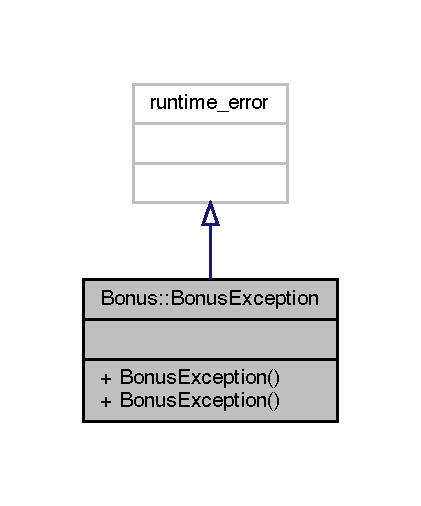
\includegraphics[width=202pt]{class_bonus_1_1_bonus_exception__inherit__graph}
\end{center}
\end{figure}


Collaboration diagram for Bonus\+::Bonus\+Exception\+:
\nopagebreak
\begin{figure}[H]
\begin{center}
\leavevmode
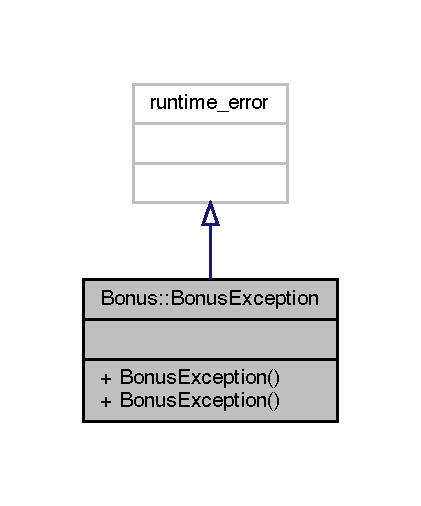
\includegraphics[width=202pt]{class_bonus_1_1_bonus_exception__coll__graph}
\end{center}
\end{figure}
\doxysubsection*{Public Member Functions}
\begin{DoxyCompactItemize}
\item 
\mbox{\hyperlink{class_bonus_1_1_bonus_exception_a82c9d131ac633d63e295f58f20a149e4}{Bonus\+Exception}} (const char $\ast$what\+Arg)
\begin{DoxyCompactList}\small\item\em Construct a new \mbox{\hyperlink{class_spawner}{Spawner}} Exception object. \end{DoxyCompactList}\end{DoxyCompactItemize}


\doxysubsection{Detailed Description}
\mbox{\hyperlink{class_bonus}{Bonus}} Exception. 

\doxysubsection{Constructor \& Destructor Documentation}
\mbox{\Hypertarget{class_bonus_1_1_bonus_exception_a82c9d131ac633d63e295f58f20a149e4}\label{class_bonus_1_1_bonus_exception_a82c9d131ac633d63e295f58f20a149e4}} 
\index{Bonus::BonusException@{Bonus::BonusException}!BonusException@{BonusException}}
\index{BonusException@{BonusException}!Bonus::BonusException@{Bonus::BonusException}}
\doxysubsubsection{\texorpdfstring{BonusException()}{BonusException()}}
{\footnotesize\ttfamily Bonus\+::\+Bonus\+Exception\+::\+Bonus\+Exception (\begin{DoxyParamCaption}\item[{const char $\ast$}]{what\+Arg }\end{DoxyParamCaption})\hspace{0.3cm}{\ttfamily [explicit]}}



Construct a new \mbox{\hyperlink{class_spawner}{Spawner}} Exception object. 


\begin{DoxyParams}{Parameters}
{\em what\+Arg} & Error message \\
\hline
\end{DoxyParams}


The documentation for this class was generated from the following files\+:\begin{DoxyCompactItemize}
\item 
includes/elements/Bonus.\+hpp\item 
srcs/elements/Bonus.\+cpp\end{DoxyCompactItemize}

\hypertarget{struct_scene_game_1_1_bonus_values}{}\doxysection{Scene\+Game\+::Bonus\+Values Struct Reference}
\label{struct_scene_game_1_1_bonus_values}\index{SceneGame::BonusValues@{SceneGame::BonusValues}}


\mbox{\hyperlink{class_bonus}{Bonus}} Information about spawn (number of bonus \& chance to spawn)  




{\ttfamily \#include $<$Scene\+Game.\+hpp$>$}



Collaboration diagram for Scene\+Game\+::Bonus\+Values\+:
\nopagebreak
\begin{figure}[H]
\begin{center}
\leavevmode
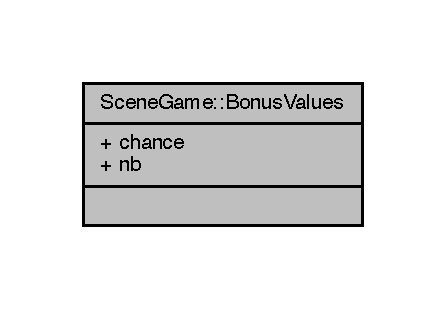
\includegraphics[width=214pt]{struct_scene_game_1_1_bonus_values__coll__graph}
\end{center}
\end{figure}
\doxysubsection*{Public Attributes}
\begin{DoxyCompactItemize}
\item 
int64\+\_\+t \mbox{\hyperlink{struct_scene_game_1_1_bonus_values_affe45b7f7a76f77c2897f3341839abfe}{chance}}
\item 
int64\+\_\+t \mbox{\hyperlink{struct_scene_game_1_1_bonus_values_a826313028a99bb7df6fef3587628c16c}{nb}}
\end{DoxyCompactItemize}


\doxysubsection{Detailed Description}
\mbox{\hyperlink{class_bonus}{Bonus}} Information about spawn (number of bonus \& chance to spawn) 

\doxysubsection{Member Data Documentation}
\mbox{\Hypertarget{struct_scene_game_1_1_bonus_values_affe45b7f7a76f77c2897f3341839abfe}\label{struct_scene_game_1_1_bonus_values_affe45b7f7a76f77c2897f3341839abfe}} 
\index{SceneGame::BonusValues@{SceneGame::BonusValues}!chance@{chance}}
\index{chance@{chance}!SceneGame::BonusValues@{SceneGame::BonusValues}}
\doxysubsubsection{\texorpdfstring{chance}{chance}}
{\footnotesize\ttfamily int64\+\_\+t Scene\+Game\+::\+Bonus\+Values\+::chance}

Chance to have a bonus \mbox{\Hypertarget{struct_scene_game_1_1_bonus_values_a826313028a99bb7df6fef3587628c16c}\label{struct_scene_game_1_1_bonus_values_a826313028a99bb7df6fef3587628c16c}} 
\index{SceneGame::BonusValues@{SceneGame::BonusValues}!nb@{nb}}
\index{nb@{nb}!SceneGame::BonusValues@{SceneGame::BonusValues}}
\doxysubsubsection{\texorpdfstring{nb}{nb}}
{\footnotesize\ttfamily int64\+\_\+t Scene\+Game\+::\+Bonus\+Values\+::nb}

Number of bonus on the level 

The documentation for this struct was generated from the following file\+:\begin{DoxyCompactItemize}
\item 
includes/scenes/Scene\+Game.\+hpp\end{DoxyCompactItemize}

\hypertarget{struct_bounding_box}{}\section{Bounding\+Box Struct Reference}
\label{struct_bounding_box}\index{Bounding\+Box@{Bounding\+Box}}


Bounding box.  




{\ttfamily \#include $<$Mesh.\+hpp$>$}



Collaboration diagram for Bounding\+Box\+:
\nopagebreak
\begin{figure}[H]
\begin{center}
\leavevmode
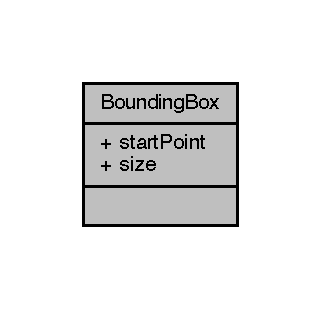
\includegraphics[width=154pt]{struct_bounding_box__coll__graph}
\end{center}
\end{figure}
\subsection*{Public Attributes}
\begin{DoxyCompactItemize}
\item 
glm\+::vec3 \hyperlink{struct_bounding_box_a4581e8476026990423d14fdd5c94b74f}{center}
\item 
float \hyperlink{struct_bounding_box_ab85c564601bd9907b4e1cd88b9e11aa2}{radius}
\end{DoxyCompactItemize}


\subsection{Detailed Description}
Bounding box. 

\subsection{Member Data Documentation}
\mbox{\Hypertarget{struct_bounding_box_a4581e8476026990423d14fdd5c94b74f}\label{struct_bounding_box_a4581e8476026990423d14fdd5c94b74f}} 
\index{Bounding\+Box@{Bounding\+Box}!center@{center}}
\index{center@{center}!Bounding\+Box@{Bounding\+Box}}
\subsubsection{\texorpdfstring{center}{center}}
{\footnotesize\ttfamily glm\+::vec3 Bounding\+Box\+::center}

The center \mbox{\Hypertarget{struct_bounding_box_ab85c564601bd9907b4e1cd88b9e11aa2}\label{struct_bounding_box_ab85c564601bd9907b4e1cd88b9e11aa2}} 
\index{Bounding\+Box@{Bounding\+Box}!radius@{radius}}
\index{radius@{radius}!Bounding\+Box@{Bounding\+Box}}
\subsubsection{\texorpdfstring{radius}{radius}}
{\footnotesize\ttfamily float Bounding\+Box\+::radius}

The radius 

The documentation for this struct was generated from the following file\+:\begin{DoxyCompactItemize}
\item 
includes/utils/opengl/Mesh.\+hpp\end{DoxyCompactItemize}

\hypertarget{class_box_collider}{}\doxysection{Box\+Collider Class Reference}
\label{class_box_collider}\index{BoxCollider@{BoxCollider}}


This is the box collider object.  




{\ttfamily \#include $<$Box\+Collider.\+hpp$>$}



Collaboration diagram for Box\+Collider\+:\nopagebreak
\begin{figure}[H]
\begin{center}
\leavevmode
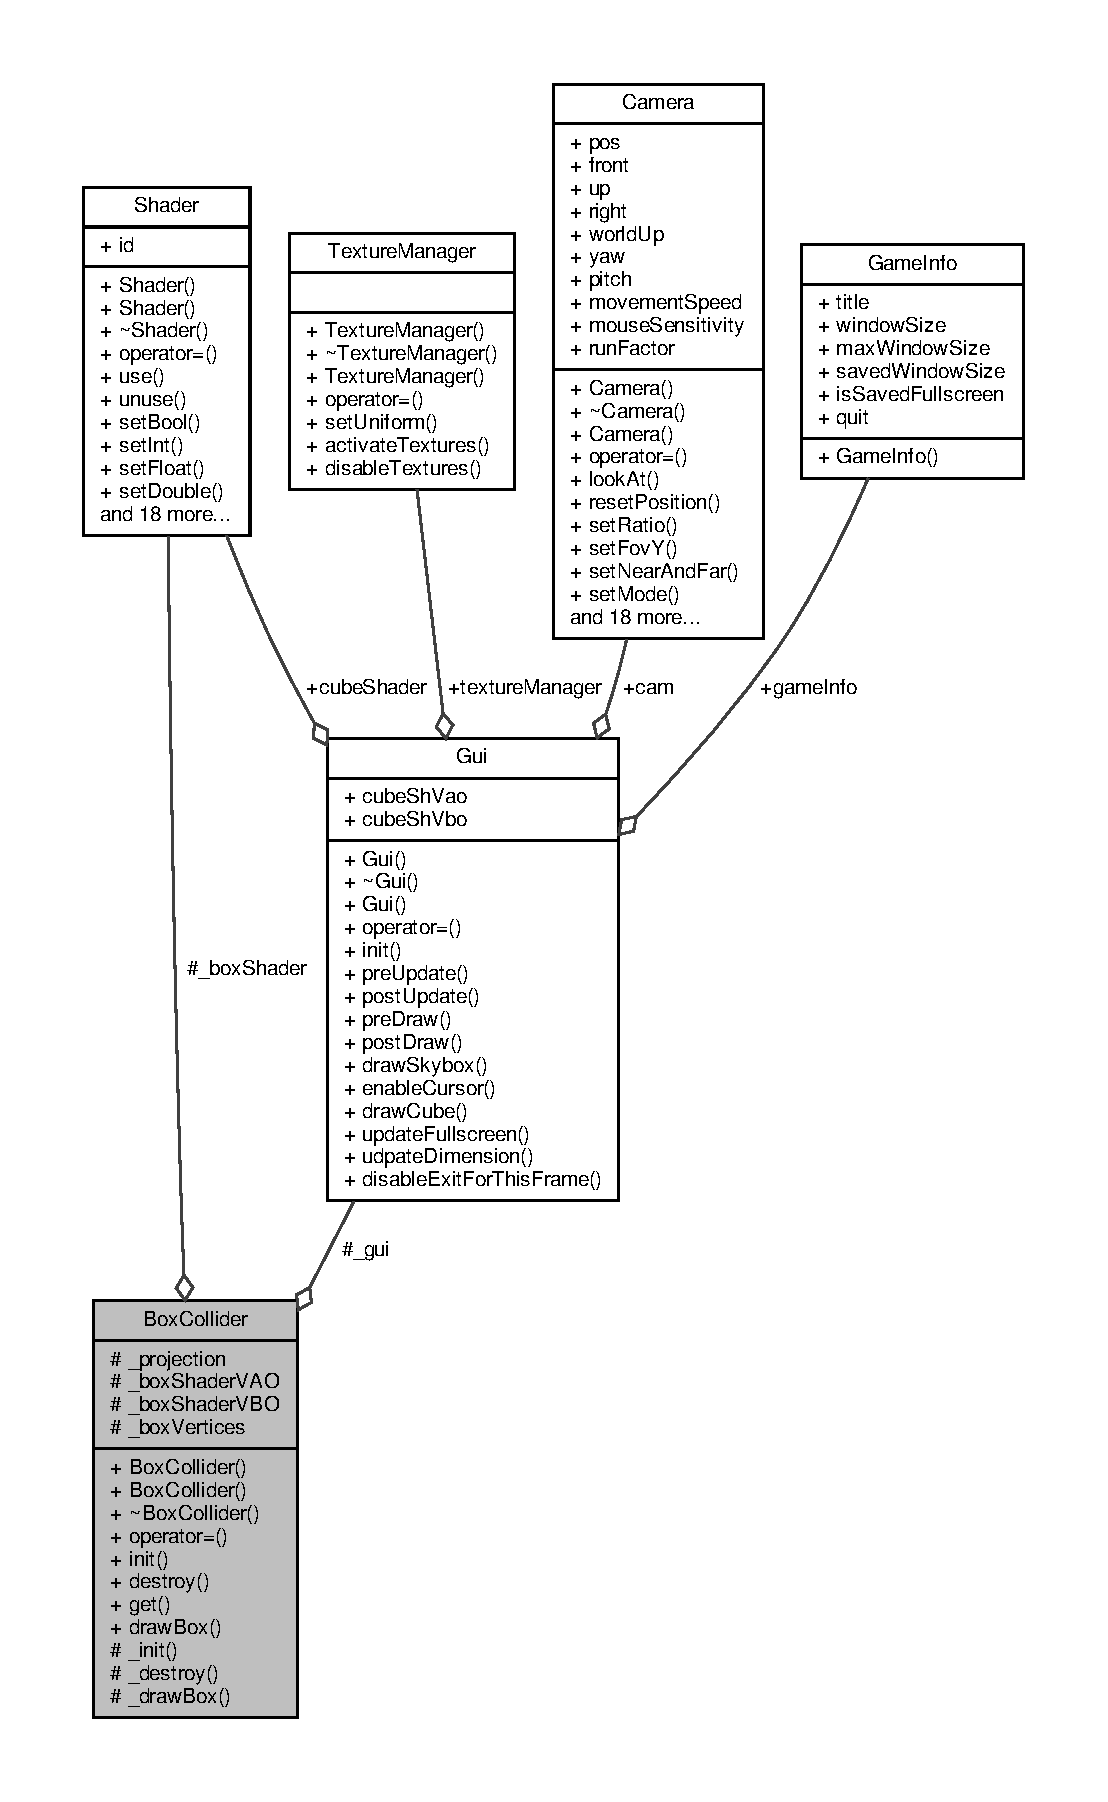
\includegraphics[height=550pt]{class_box_collider__coll__graph}
\end{center}
\end{figure}
\doxysubsection*{Public Member Functions}
\begin{DoxyCompactItemize}
\item 
\mbox{\Hypertarget{class_box_collider_aa8358aaf4f5fae5446ebdf0b303ccce3}\label{class_box_collider_aa8358aaf4f5fae5446ebdf0b303ccce3}} 
\mbox{\hyperlink{class_box_collider_aa8358aaf4f5fae5446ebdf0b303ccce3}{Box\+Collider}} ()
\begin{DoxyCompactList}\small\item\em Construct a new Box Collider\+:\+: Box Collider object. \end{DoxyCompactList}\item 
\mbox{\hyperlink{class_box_collider_a79511f75725470715ff72c4b4622de21}{Box\+Collider}} (\mbox{\hyperlink{class_box_collider}{Box\+Collider}} const \&src)
\begin{DoxyCompactList}\small\item\em Construct a new Box Collider\+:\+: Box Collider object. \end{DoxyCompactList}\item 
\mbox{\Hypertarget{class_box_collider_a8c33dbb4325d76d441de38b7c4ae43af}\label{class_box_collider_a8c33dbb4325d76d441de38b7c4ae43af}} 
virtual \mbox{\hyperlink{class_box_collider_a8c33dbb4325d76d441de38b7c4ae43af}{$\sim$\+Box\+Collider}} ()
\begin{DoxyCompactList}\small\item\em Destroy the Box Collider\+:\+: Box Collider object. \end{DoxyCompactList}\item 
\mbox{\hyperlink{class_box_collider}{Box\+Collider}} \& \mbox{\hyperlink{class_box_collider_a785e2defc2d9deab26589149262ff114}{operator=}} (\mbox{\hyperlink{class_box_collider}{Box\+Collider}} const \&rhs)
\begin{DoxyCompactList}\small\item\em Copy this object. \end{DoxyCompactList}\end{DoxyCompactItemize}
\doxysubsection*{Static Public Member Functions}
\begin{DoxyCompactItemize}
\item 
static bool \mbox{\hyperlink{class_box_collider_a6f8b8b22f9845496c422236140818209}{init}} (\mbox{\hyperlink{class_gui}{Gui}} $\ast$gui)
\begin{DoxyCompactList}\small\item\em Init the \mbox{\hyperlink{class_box_collider}{Box\+Collider}} object (call only once) \end{DoxyCompactList}\item 
static bool \mbox{\hyperlink{class_box_collider_a3fd8069de8cba507e4b3ac66b995d632}{destroy}} ()
\begin{DoxyCompactList}\small\item\em Destroy the \mbox{\hyperlink{class_box_collider}{Box\+Collider}} object (call only once) \end{DoxyCompactList}\item 
static \mbox{\hyperlink{class_box_collider}{Box\+Collider}} \& \mbox{\hyperlink{class_box_collider_a830532bce2aa57c773c8d7617cc8fe2b}{get}} ()
\begin{DoxyCompactList}\small\item\em Get the instance of \mbox{\hyperlink{class_box_collider}{Box\+Collider}} object. \end{DoxyCompactList}\item 
static bool \mbox{\hyperlink{class_box_collider_a4a5eccd572ec94bf11fab22fa24765ac}{draw\+Box}} (glm\+::vec3 pos, glm\+::vec3 size, glm\+::vec4 color=\{0, 0, 0, 1\})
\begin{DoxyCompactList}\small\item\em Draw a box collider on the screen. \end{DoxyCompactList}\end{DoxyCompactItemize}
\doxysubsection*{Protected Member Functions}
\begin{DoxyCompactItemize}
\item 
bool \mbox{\hyperlink{class_box_collider_a5782997a36f86f46a83d4f528c7ae391}{\+\_\+init}} (\mbox{\hyperlink{class_gui}{Gui}} $\ast$gui)
\begin{DoxyCompactList}\small\item\em Init the \mbox{\hyperlink{class_box_collider}{Box\+Collider}} object (call only once) \end{DoxyCompactList}\item 
bool \mbox{\hyperlink{class_box_collider_a447744df9a4567cab18eb6aabc8fd1c6}{\+\_\+destroy}} ()
\begin{DoxyCompactList}\small\item\em Destroy the \mbox{\hyperlink{class_box_collider}{Box\+Collider}} object (call only once) \end{DoxyCompactList}\item 
bool \mbox{\hyperlink{class_box_collider_af71d692699a39ea2bc5ee61384d533e9}{\+\_\+draw\+Box}} (glm\+::vec3 pos, glm\+::vec3 size, glm\+::vec4 color)
\begin{DoxyCompactList}\small\item\em Draw a box collider on the screen. \end{DoxyCompactList}\end{DoxyCompactItemize}
\doxysubsection*{Protected Attributes}
\begin{DoxyCompactItemize}
\item 
\mbox{\hyperlink{class_gui}{Gui}} $\ast$ \mbox{\hyperlink{class_box_collider_a79878a3379cc1710aec75057373dc3d1}{\+\_\+gui}}
\item 
glm\+::mat4 \mbox{\hyperlink{class_box_collider_a1eb52f9eec4a732c48b12c074ce23c29}{\+\_\+projection}}
\item 
\mbox{\hyperlink{class_shader}{Shader}} $\ast$ \mbox{\hyperlink{class_box_collider_ab8642b5f05444676fb3ef9bccda8ce34}{\+\_\+box\+Shader}}
\item 
uint32\+\_\+t \mbox{\hyperlink{class_box_collider_ab57de816c107545459f5b920688f9cc6}{\+\_\+box\+Shader\+V\+AO}}
\item 
uint32\+\_\+t \mbox{\hyperlink{class_box_collider_af2ac832bfc806b578a9b9be7d39c7946}{\+\_\+box\+Shader\+V\+BO}}
\end{DoxyCompactItemize}
\doxysubsection*{Static Protected Attributes}
\begin{DoxyCompactItemize}
\item 
static const float \mbox{\hyperlink{class_box_collider_a8fc69f37cbd732dfc24a2e97f92f161e}{\+\_\+box\+Vertices}} \mbox{[}$\,$\mbox{]}
\end{DoxyCompactItemize}


\doxysubsection{Detailed Description}
This is the box collider object. 

\doxysubsection{Constructor \& Destructor Documentation}
\mbox{\Hypertarget{class_box_collider_a79511f75725470715ff72c4b4622de21}\label{class_box_collider_a79511f75725470715ff72c4b4622de21}} 
\index{BoxCollider@{BoxCollider}!BoxCollider@{BoxCollider}}
\index{BoxCollider@{BoxCollider}!BoxCollider@{BoxCollider}}
\doxysubsubsection{\texorpdfstring{BoxCollider()}{BoxCollider()}}
{\footnotesize\ttfamily Box\+Collider\+::\+Box\+Collider (\begin{DoxyParamCaption}\item[{\mbox{\hyperlink{class_box_collider}{Box\+Collider}} const \&}]{src }\end{DoxyParamCaption})}



Construct a new Box Collider\+:\+: Box Collider object. 


\begin{DoxyParams}{Parameters}
{\em src} & The object to do the copy \\
\hline
\end{DoxyParams}


\doxysubsection{Member Function Documentation}
\mbox{\Hypertarget{class_box_collider_a447744df9a4567cab18eb6aabc8fd1c6}\label{class_box_collider_a447744df9a4567cab18eb6aabc8fd1c6}} 
\index{BoxCollider@{BoxCollider}!\_destroy@{\_destroy}}
\index{\_destroy@{\_destroy}!BoxCollider@{BoxCollider}}
\doxysubsubsection{\texorpdfstring{\_destroy()}{\_destroy()}}
{\footnotesize\ttfamily bool Box\+Collider\+::\+\_\+destroy (\begin{DoxyParamCaption}{ }\end{DoxyParamCaption})\hspace{0.3cm}{\ttfamily [protected]}}



Destroy the \mbox{\hyperlink{class_box_collider}{Box\+Collider}} object (call only once) 

\begin{DoxyReturn}{Returns}
false If failed 
\end{DoxyReturn}
\mbox{\Hypertarget{class_box_collider_af71d692699a39ea2bc5ee61384d533e9}\label{class_box_collider_af71d692699a39ea2bc5ee61384d533e9}} 
\index{BoxCollider@{BoxCollider}!\_drawBox@{\_drawBox}}
\index{\_drawBox@{\_drawBox}!BoxCollider@{BoxCollider}}
\doxysubsubsection{\texorpdfstring{\_drawBox()}{\_drawBox()}}
{\footnotesize\ttfamily bool Box\+Collider\+::\+\_\+draw\+Box (\begin{DoxyParamCaption}\item[{glm\+::vec3}]{pos,  }\item[{glm\+::vec3}]{size,  }\item[{glm\+::vec4}]{color }\end{DoxyParamCaption})\hspace{0.3cm}{\ttfamily [protected]}}



Draw a box collider on the screen. 


\begin{DoxyParams}{Parameters}
{\em pos} & The position \\
\hline
{\em size} & The size \\
\hline
{\em color} & The color \\
\hline
\end{DoxyParams}
\mbox{\Hypertarget{class_box_collider_a5782997a36f86f46a83d4f528c7ae391}\label{class_box_collider_a5782997a36f86f46a83d4f528c7ae391}} 
\index{BoxCollider@{BoxCollider}!\_init@{\_init}}
\index{\_init@{\_init}!BoxCollider@{BoxCollider}}
\doxysubsubsection{\texorpdfstring{\_init()}{\_init()}}
{\footnotesize\ttfamily bool Box\+Collider\+::\+\_\+init (\begin{DoxyParamCaption}\item[{\mbox{\hyperlink{class_gui}{Gui}} $\ast$}]{gui }\end{DoxyParamCaption})\hspace{0.3cm}{\ttfamily [protected]}}



Init the \mbox{\hyperlink{class_box_collider}{Box\+Collider}} object (call only once) 

\begin{DoxyReturn}{Returns}
false If failed 
\end{DoxyReturn}
\mbox{\Hypertarget{class_box_collider_a3fd8069de8cba507e4b3ac66b995d632}\label{class_box_collider_a3fd8069de8cba507e4b3ac66b995d632}} 
\index{BoxCollider@{BoxCollider}!destroy@{destroy}}
\index{destroy@{destroy}!BoxCollider@{BoxCollider}}
\doxysubsubsection{\texorpdfstring{destroy()}{destroy()}}
{\footnotesize\ttfamily bool Box\+Collider\+::destroy (\begin{DoxyParamCaption}{ }\end{DoxyParamCaption})\hspace{0.3cm}{\ttfamily [static]}}



Destroy the \mbox{\hyperlink{class_box_collider}{Box\+Collider}} object (call only once) 

\begin{DoxyReturn}{Returns}
false If failed 
\end{DoxyReturn}
\mbox{\Hypertarget{class_box_collider_a4a5eccd572ec94bf11fab22fa24765ac}\label{class_box_collider_a4a5eccd572ec94bf11fab22fa24765ac}} 
\index{BoxCollider@{BoxCollider}!drawBox@{drawBox}}
\index{drawBox@{drawBox}!BoxCollider@{BoxCollider}}
\doxysubsubsection{\texorpdfstring{drawBox()}{drawBox()}}
{\footnotesize\ttfamily bool Box\+Collider\+::draw\+Box (\begin{DoxyParamCaption}\item[{glm\+::vec3}]{pos,  }\item[{glm\+::vec3}]{size,  }\item[{glm\+::vec4}]{color = {\ttfamily \{0,~0,~0,~1\}} }\end{DoxyParamCaption})\hspace{0.3cm}{\ttfamily [static]}}



Draw a box collider on the screen. 


\begin{DoxyParams}{Parameters}
{\em pos} & The position \\
\hline
{\em size} & The size \\
\hline
{\em color} & The color \\
\hline
\end{DoxyParams}
\mbox{\Hypertarget{class_box_collider_a830532bce2aa57c773c8d7617cc8fe2b}\label{class_box_collider_a830532bce2aa57c773c8d7617cc8fe2b}} 
\index{BoxCollider@{BoxCollider}!get@{get}}
\index{get@{get}!BoxCollider@{BoxCollider}}
\doxysubsubsection{\texorpdfstring{get()}{get()}}
{\footnotesize\ttfamily \mbox{\hyperlink{class_box_collider}{Box\+Collider}} \& Box\+Collider\+::get (\begin{DoxyParamCaption}{ }\end{DoxyParamCaption})\hspace{0.3cm}{\ttfamily [static]}}



Get the instance of \mbox{\hyperlink{class_box_collider}{Box\+Collider}} object. 

\begin{DoxyReturn}{Returns}
\mbox{\hyperlink{class_box_collider}{Box\+Collider}}\& The instance 
\end{DoxyReturn}
\mbox{\Hypertarget{class_box_collider_a6f8b8b22f9845496c422236140818209}\label{class_box_collider_a6f8b8b22f9845496c422236140818209}} 
\index{BoxCollider@{BoxCollider}!init@{init}}
\index{init@{init}!BoxCollider@{BoxCollider}}
\doxysubsubsection{\texorpdfstring{init()}{init()}}
{\footnotesize\ttfamily bool Box\+Collider\+::init (\begin{DoxyParamCaption}\item[{\mbox{\hyperlink{class_gui}{Gui}} $\ast$}]{gui }\end{DoxyParamCaption})\hspace{0.3cm}{\ttfamily [static]}}



Init the \mbox{\hyperlink{class_box_collider}{Box\+Collider}} object (call only once) 

\begin{DoxyReturn}{Returns}
false If failed 
\end{DoxyReturn}
\mbox{\Hypertarget{class_box_collider_a785e2defc2d9deab26589149262ff114}\label{class_box_collider_a785e2defc2d9deab26589149262ff114}} 
\index{BoxCollider@{BoxCollider}!operator=@{operator=}}
\index{operator=@{operator=}!BoxCollider@{BoxCollider}}
\doxysubsubsection{\texorpdfstring{operator=()}{operator=()}}
{\footnotesize\ttfamily \mbox{\hyperlink{class_box_collider}{Box\+Collider}} \& Box\+Collider\+::operator= (\begin{DoxyParamCaption}\item[{\mbox{\hyperlink{class_box_collider}{Box\+Collider}} const \&}]{rhs }\end{DoxyParamCaption})}



Copy this object. 


\begin{DoxyParams}{Parameters}
{\em rhs} & The object to copy \\
\hline
\end{DoxyParams}
\begin{DoxyReturn}{Returns}
\mbox{\hyperlink{class_box_collider}{Box\+Collider}}\& A reference to the copied object 
\end{DoxyReturn}


\doxysubsection{Member Data Documentation}
\mbox{\Hypertarget{class_box_collider_ab8642b5f05444676fb3ef9bccda8ce34}\label{class_box_collider_ab8642b5f05444676fb3ef9bccda8ce34}} 
\index{BoxCollider@{BoxCollider}!\_boxShader@{\_boxShader}}
\index{\_boxShader@{\_boxShader}!BoxCollider@{BoxCollider}}
\doxysubsubsection{\texorpdfstring{\_boxShader}{\_boxShader}}
{\footnotesize\ttfamily \mbox{\hyperlink{class_shader}{Shader}}$\ast$ Box\+Collider\+::\+\_\+box\+Shader\hspace{0.3cm}{\ttfamily [protected]}}

\mbox{\hyperlink{class_shader}{Shader}} \mbox{\Hypertarget{class_box_collider_ab57de816c107545459f5b920688f9cc6}\label{class_box_collider_ab57de816c107545459f5b920688f9cc6}} 
\index{BoxCollider@{BoxCollider}!\_boxShaderVAO@{\_boxShaderVAO}}
\index{\_boxShaderVAO@{\_boxShaderVAO}!BoxCollider@{BoxCollider}}
\doxysubsubsection{\texorpdfstring{\_boxShaderVAO}{\_boxShaderVAO}}
{\footnotesize\ttfamily uint32\+\_\+t Box\+Collider\+::\+\_\+box\+Shader\+V\+AO\hspace{0.3cm}{\ttfamily [protected]}}

\mbox{\hyperlink{struct_vertex}{Vertex}} Array Objects \mbox{\Hypertarget{class_box_collider_af2ac832bfc806b578a9b9be7d39c7946}\label{class_box_collider_af2ac832bfc806b578a9b9be7d39c7946}} 
\index{BoxCollider@{BoxCollider}!\_boxShaderVBO@{\_boxShaderVBO}}
\index{\_boxShaderVBO@{\_boxShaderVBO}!BoxCollider@{BoxCollider}}
\doxysubsubsection{\texorpdfstring{\_boxShaderVBO}{\_boxShaderVBO}}
{\footnotesize\ttfamily uint32\+\_\+t Box\+Collider\+::\+\_\+box\+Shader\+V\+BO\hspace{0.3cm}{\ttfamily [protected]}}

\mbox{\hyperlink{struct_vertex}{Vertex}} Buffer Objects \mbox{\Hypertarget{class_box_collider_a8fc69f37cbd732dfc24a2e97f92f161e}\label{class_box_collider_a8fc69f37cbd732dfc24a2e97f92f161e}} 
\index{BoxCollider@{BoxCollider}!\_boxVertices@{\_boxVertices}}
\index{\_boxVertices@{\_boxVertices}!BoxCollider@{BoxCollider}}
\doxysubsubsection{\texorpdfstring{\_boxVertices}{\_boxVertices}}
{\footnotesize\ttfamily const float Box\+Collider\+::\+\_\+box\+Vertices\hspace{0.3cm}{\ttfamily [static]}, {\ttfamily [protected]}}

Collider vertices \mbox{\Hypertarget{class_box_collider_a79878a3379cc1710aec75057373dc3d1}\label{class_box_collider_a79878a3379cc1710aec75057373dc3d1}} 
\index{BoxCollider@{BoxCollider}!\_gui@{\_gui}}
\index{\_gui@{\_gui}!BoxCollider@{BoxCollider}}
\doxysubsubsection{\texorpdfstring{\_gui}{\_gui}}
{\footnotesize\ttfamily \mbox{\hyperlink{class_gui}{Gui}}$\ast$ Box\+Collider\+::\+\_\+gui\hspace{0.3cm}{\ttfamily [protected]}}

Ref to G\+UI object \mbox{\Hypertarget{class_box_collider_a1eb52f9eec4a732c48b12c074ce23c29}\label{class_box_collider_a1eb52f9eec4a732c48b12c074ce23c29}} 
\index{BoxCollider@{BoxCollider}!\_projection@{\_projection}}
\index{\_projection@{\_projection}!BoxCollider@{BoxCollider}}
\doxysubsubsection{\texorpdfstring{\_projection}{\_projection}}
{\footnotesize\ttfamily glm\+::mat4 Box\+Collider\+::\+\_\+projection\hspace{0.3cm}{\ttfamily [protected]}}

projection matrix 

The documentation for this class was generated from the following files\+:\begin{DoxyCompactItemize}
\item 
includes/gui/Box\+Collider.\+hpp\item 
srcs/gui/Box\+Collider.\+cpp\end{DoxyCompactItemize}

\hypertarget{class_button_image_u_i}{}\doxysection{Button\+Image\+UI Class Reference}
\label{class_button_image_u_i}\index{ButtonImageUI@{ButtonImageUI}}


this is the UI for button image  




{\ttfamily \#include $<$Button\+Image\+U\+I.\+hpp$>$}



Inheritance diagram for Button\+Image\+UI\+:\nopagebreak
\begin{figure}[H]
\begin{center}
\leavevmode
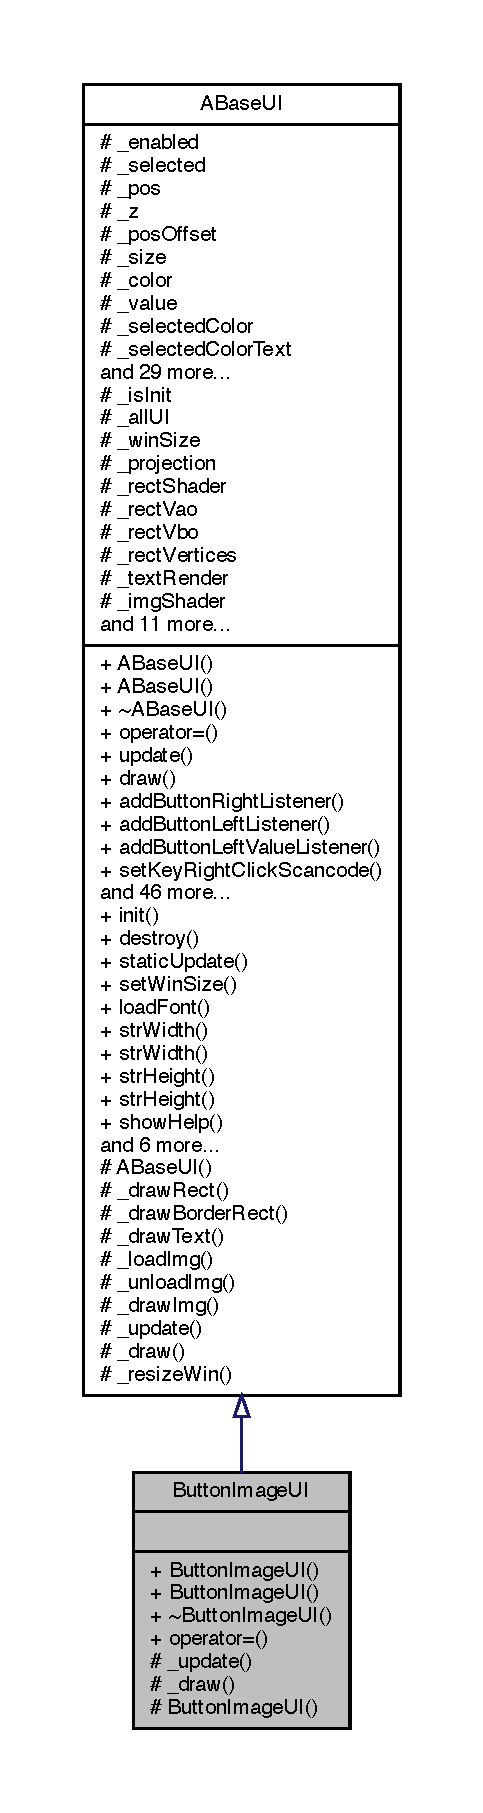
\includegraphics[height=550pt]{class_button_image_u_i__inherit__graph}
\end{center}
\end{figure}


Collaboration diagram for Button\+Image\+UI\+:\nopagebreak
\begin{figure}[H]
\begin{center}
\leavevmode
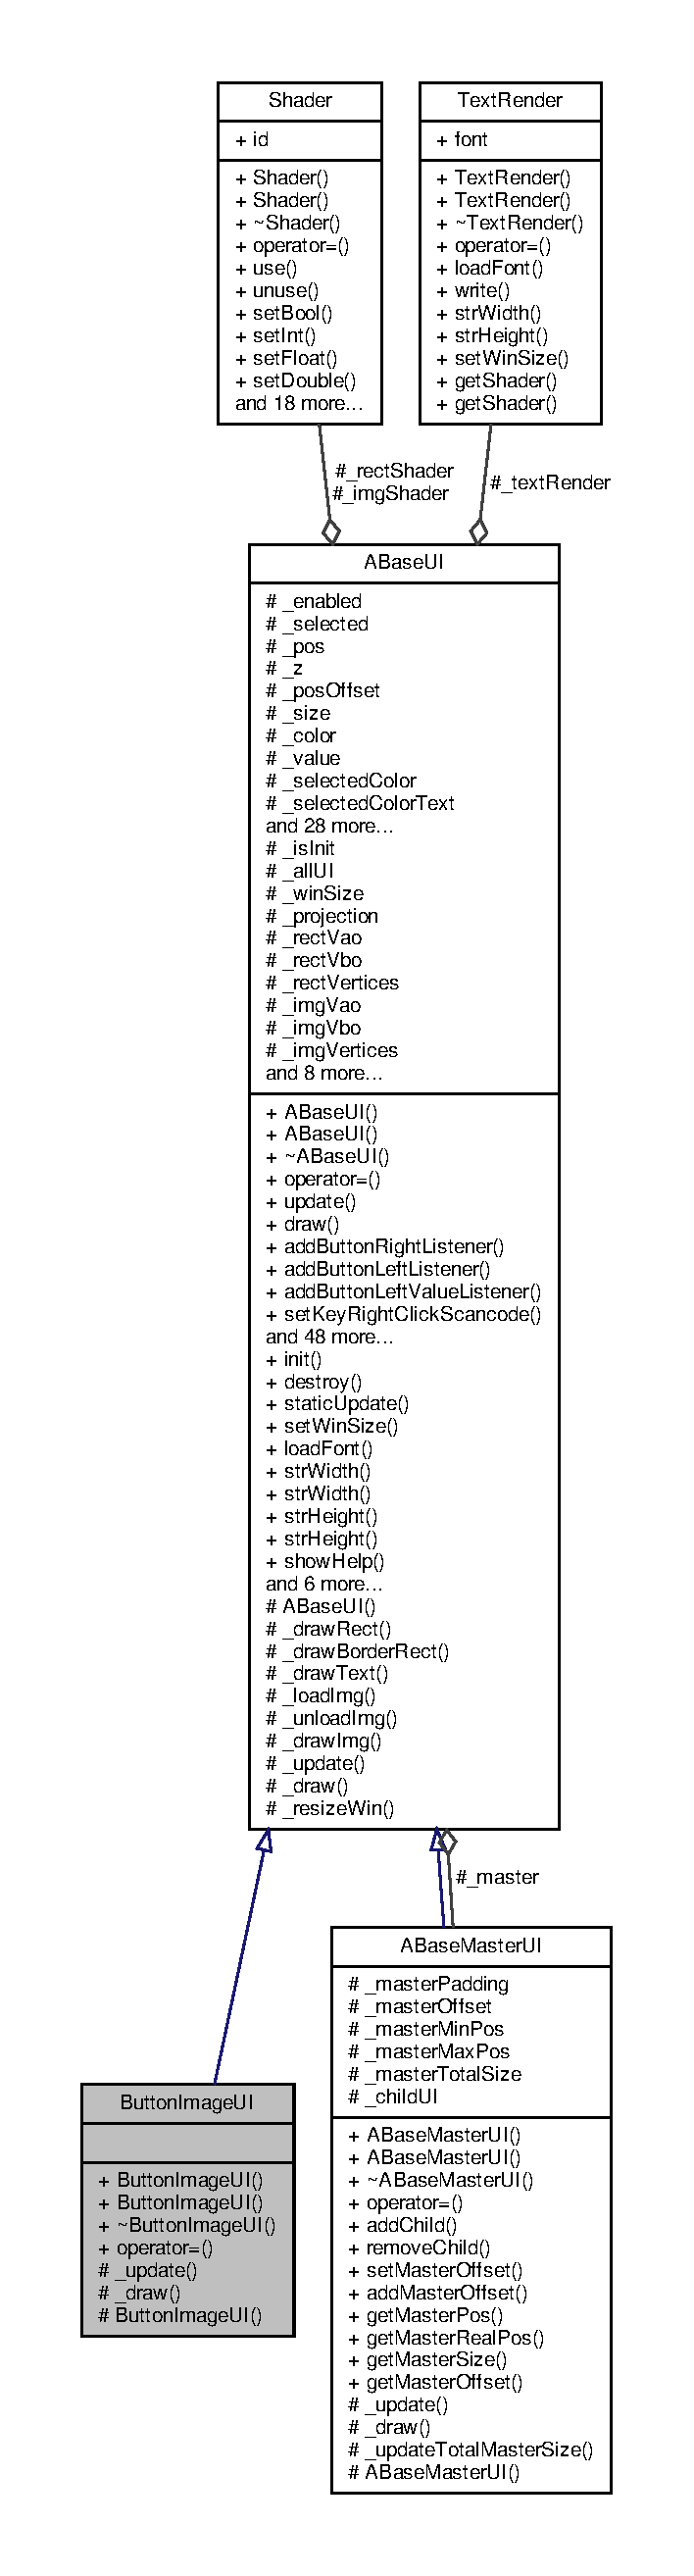
\includegraphics[height=550pt]{class_button_image_u_i__coll__graph}
\end{center}
\end{figure}
\doxysubsection*{Public Member Functions}
\begin{DoxyCompactItemize}
\item 
\mbox{\Hypertarget{class_button_image_u_i_a23d0abf7c75a4660cc94a0e615d1931c}\label{class_button_image_u_i_a23d0abf7c75a4660cc94a0e615d1931c}} 
{\bfseries Button\+Image\+UI} (glm\+::vec2 pos, glm\+::vec2 size, std\+::string const \&filename)
\item 
\mbox{\Hypertarget{class_button_image_u_i_abeb26451e576873e82b443944e241616}\label{class_button_image_u_i_abeb26451e576873e82b443944e241616}} 
{\bfseries Button\+Image\+UI} (\mbox{\hyperlink{class_button_image_u_i}{Button\+Image\+UI}} const \&src)
\item 
\mbox{\Hypertarget{class_button_image_u_i_a1915cfb56b96a85b1c0fad64508fe9f3}\label{class_button_image_u_i_a1915cfb56b96a85b1c0fad64508fe9f3}} 
\mbox{\hyperlink{class_button_image_u_i}{Button\+Image\+UI}} \& {\bfseries operator=} (\mbox{\hyperlink{class_button_image_u_i}{Button\+Image\+UI}} const \&rhs)
\end{DoxyCompactItemize}
\doxysubsection*{Protected Member Functions}
\begin{DoxyCompactItemize}
\item 
\mbox{\Hypertarget{class_button_image_u_i_a9f0a37050956baa365de40daf3b05bb5}\label{class_button_image_u_i_a9f0a37050956baa365de40daf3b05bb5}} 
virtual void \mbox{\hyperlink{class_button_image_u_i_a9f0a37050956baa365de40daf3b05bb5}{\+\_\+update}} ()
\begin{DoxyCompactList}\small\item\em this is the base update function of UI objects \end{DoxyCompactList}\item 
\mbox{\Hypertarget{class_button_image_u_i_aea117caa97ce8cb0d888776a9872a405}\label{class_button_image_u_i_aea117caa97ce8cb0d888776a9872a405}} 
virtual void \mbox{\hyperlink{class_button_image_u_i_aea117caa97ce8cb0d888776a9872a405}{\+\_\+draw}} ()
\begin{DoxyCompactList}\small\item\em this is the draw function for UI /!\textbackslash{} -\/$>$ you need to draw in the reverse order (draw at first the element on the top) \end{DoxyCompactList}\end{DoxyCompactItemize}
\doxysubsection*{Additional Inherited Members}


\doxysubsection{Detailed Description}
this is the UI for button image 

The documentation for this class was generated from the following files\+:\begin{DoxyCompactItemize}
\item 
includes/utils/opengl/\+U\+I/Button\+Image\+U\+I.\+hpp\item 
srcs/utils/opengl/\+U\+I/Button\+Image\+U\+I.\+cpp\end{DoxyCompactItemize}

\hypertarget{struct_scene_end_game_1_1_buttons_states}{}\section{Scene\+End\+Game\+:\+:Buttons\+States Struct Reference}
\label{struct_scene_end_game_1_1_buttons_states}\index{Scene\+End\+Game\+::\+Buttons\+States@{Scene\+End\+Game\+::\+Buttons\+States}}


All buttons states.  




{\ttfamily \#include $<$Scene\+End\+Game.\+hpp$>$}



Collaboration diagram for Scene\+End\+Game\+:\+:Buttons\+States\+:
\nopagebreak
\begin{figure}[H]
\begin{center}
\leavevmode
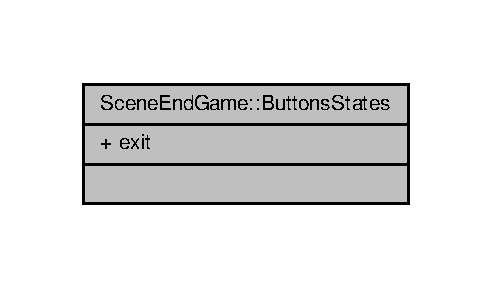
\includegraphics[width=236pt]{struct_scene_end_game_1_1_buttons_states__coll__graph}
\end{center}
\end{figure}
\subsection*{Public Attributes}
\begin{DoxyCompactItemize}
\item 
bool \hyperlink{struct_scene_end_game_1_1_buttons_states_a7e876bf38fa9a782a44abb5fe38c0a6e}{exit}
\end{DoxyCompactItemize}


\subsection{Detailed Description}
All buttons states. 

\subsection{Member Data Documentation}
\mbox{\Hypertarget{struct_scene_end_game_1_1_buttons_states_a7e876bf38fa9a782a44abb5fe38c0a6e}\label{struct_scene_end_game_1_1_buttons_states_a7e876bf38fa9a782a44abb5fe38c0a6e}} 
\index{Scene\+End\+Game\+::\+Buttons\+States@{Scene\+End\+Game\+::\+Buttons\+States}!exit@{exit}}
\index{exit@{exit}!Scene\+End\+Game\+::\+Buttons\+States@{Scene\+End\+Game\+::\+Buttons\+States}}
\subsubsection{\texorpdfstring{exit}{exit}}
{\footnotesize\ttfamily bool Scene\+End\+Game\+::\+Buttons\+States\+::exit}

True if we clicked on the exit button 

The documentation for this struct was generated from the following file\+:\begin{DoxyCompactItemize}
\item 
includes/scenes/Scene\+End\+Game.\+hpp\end{DoxyCompactItemize}

\hypertarget{struct_scene_exit_1_1_buttons_states}{}\doxysection{Scene\+Exit\+::Buttons\+States Struct Reference}
\label{struct_scene_exit_1_1_buttons_states}\index{SceneExit::ButtonsStates@{SceneExit::ButtonsStates}}


Collaboration diagram for Scene\+Exit\+::Buttons\+States\+:\nopagebreak
\begin{figure}[H]
\begin{center}
\leavevmode
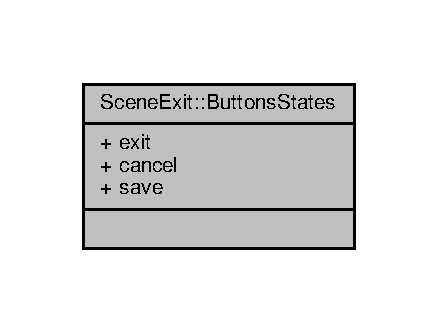
\includegraphics[width=210pt]{struct_scene_exit_1_1_buttons_states__coll__graph}
\end{center}
\end{figure}
\doxysubsection*{Public Attributes}
\begin{DoxyCompactItemize}
\item 
\mbox{\Hypertarget{struct_scene_exit_1_1_buttons_states_a035e7a8f4ed3945bd01f050a1589998b}\label{struct_scene_exit_1_1_buttons_states_a035e7a8f4ed3945bd01f050a1589998b}} 
bool {\bfseries exit}
\item 
\mbox{\Hypertarget{struct_scene_exit_1_1_buttons_states_a038f086f52088417dcbb86534a23bdaf}\label{struct_scene_exit_1_1_buttons_states_a038f086f52088417dcbb86534a23bdaf}} 
bool {\bfseries cancel}
\item 
\mbox{\Hypertarget{struct_scene_exit_1_1_buttons_states_a270d56195b6cee3befa788006aa40371}\label{struct_scene_exit_1_1_buttons_states_a270d56195b6cee3befa788006aa40371}} 
bool {\bfseries save}
\end{DoxyCompactItemize}


The documentation for this struct was generated from the following file\+:\begin{DoxyCompactItemize}
\item 
includes/scenes/Scene\+Exit.\+hpp\end{DoxyCompactItemize}

\hypertarget{struct_scene_game_over_1_1_buttons_states}{}\doxysection{Scene\+Game\+Over\+::Buttons\+States Struct Reference}
\label{struct_scene_game_over_1_1_buttons_states}\index{SceneGameOver::ButtonsStates@{SceneGameOver::ButtonsStates}}


All buttons states.  




{\ttfamily \#include $<$Scene\+Game\+Over.\+hpp$>$}



Collaboration diagram for Scene\+Game\+Over\+::Buttons\+States\+:\nopagebreak
\begin{figure}[H]
\begin{center}
\leavevmode
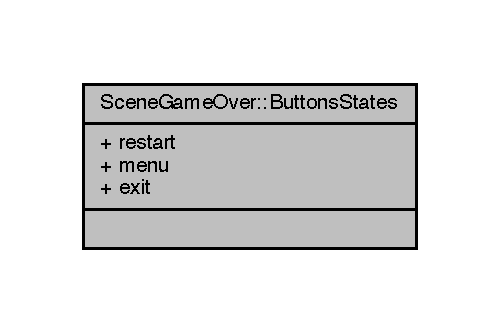
\includegraphics[width=240pt]{struct_scene_game_over_1_1_buttons_states__coll__graph}
\end{center}
\end{figure}
\doxysubsection*{Public Attributes}
\begin{DoxyCompactItemize}
\item 
bool \mbox{\hyperlink{struct_scene_game_over_1_1_buttons_states_afc64da074de682be7f40ba241d41728e}{restart}}
\item 
bool \mbox{\hyperlink{struct_scene_game_over_1_1_buttons_states_a3cec246cce96410ef3860b9af81347b3}{menu}}
\item 
bool \mbox{\hyperlink{struct_scene_game_over_1_1_buttons_states_a32b0d6225b1fdbe9f27359c528e58811}{exit}}
\end{DoxyCompactItemize}


\doxysubsection{Detailed Description}
All buttons states. 

\doxysubsection{Member Data Documentation}
\mbox{\Hypertarget{struct_scene_game_over_1_1_buttons_states_a32b0d6225b1fdbe9f27359c528e58811}\label{struct_scene_game_over_1_1_buttons_states_a32b0d6225b1fdbe9f27359c528e58811}} 
\index{SceneGameOver::ButtonsStates@{SceneGameOver::ButtonsStates}!exit@{exit}}
\index{exit@{exit}!SceneGameOver::ButtonsStates@{SceneGameOver::ButtonsStates}}
\doxysubsubsection{\texorpdfstring{exit}{exit}}
{\footnotesize\ttfamily bool Scene\+Game\+Over\+::\+Buttons\+States\+::exit}

True if we click on the button exit \mbox{\Hypertarget{struct_scene_game_over_1_1_buttons_states_a3cec246cce96410ef3860b9af81347b3}\label{struct_scene_game_over_1_1_buttons_states_a3cec246cce96410ef3860b9af81347b3}} 
\index{SceneGameOver::ButtonsStates@{SceneGameOver::ButtonsStates}!menu@{menu}}
\index{menu@{menu}!SceneGameOver::ButtonsStates@{SceneGameOver::ButtonsStates}}
\doxysubsubsection{\texorpdfstring{menu}{menu}}
{\footnotesize\ttfamily bool Scene\+Game\+Over\+::\+Buttons\+States\+::menu}

True if we click on the button menu \mbox{\Hypertarget{struct_scene_game_over_1_1_buttons_states_afc64da074de682be7f40ba241d41728e}\label{struct_scene_game_over_1_1_buttons_states_afc64da074de682be7f40ba241d41728e}} 
\index{SceneGameOver::ButtonsStates@{SceneGameOver::ButtonsStates}!restart@{restart}}
\index{restart@{restart}!SceneGameOver::ButtonsStates@{SceneGameOver::ButtonsStates}}
\doxysubsubsection{\texorpdfstring{restart}{restart}}
{\footnotesize\ttfamily bool Scene\+Game\+Over\+::\+Buttons\+States\+::restart}

True if we click on the button restart 

The documentation for this struct was generated from the following file\+:\begin{DoxyCompactItemize}
\item 
includes/scenes/Scene\+Game\+Over.\+hpp\end{DoxyCompactItemize}

\hypertarget{struct_scene_help_1_1_buttons_states}{}\doxysection{Scene\+Help\+::Buttons\+States Struct Reference}
\label{struct_scene_help_1_1_buttons_states}\index{SceneHelp::ButtonsStates@{SceneHelp::ButtonsStates}}


All buttons states.  




{\ttfamily \#include $<$Scene\+Help.\+hpp$>$}



Collaboration diagram for Scene\+Help\+::Buttons\+States\+:
\nopagebreak
\begin{figure}[H]
\begin{center}
\leavevmode
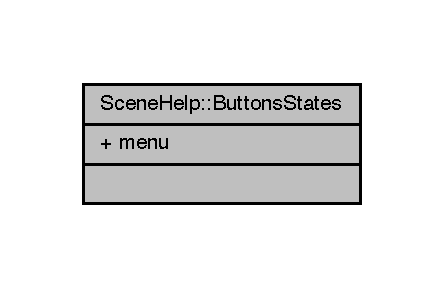
\includegraphics[width=213pt]{struct_scene_help_1_1_buttons_states__coll__graph}
\end{center}
\end{figure}
\doxysubsection*{Public Attributes}
\begin{DoxyCompactItemize}
\item 
bool \mbox{\hyperlink{struct_scene_help_1_1_buttons_states_a73c6dc843eeb08f4c029ef6d2ef7c9c7}{menu}}
\end{DoxyCompactItemize}


\doxysubsection{Detailed Description}
All buttons states. 

\doxysubsection{Member Data Documentation}
\mbox{\Hypertarget{struct_scene_help_1_1_buttons_states_a73c6dc843eeb08f4c029ef6d2ef7c9c7}\label{struct_scene_help_1_1_buttons_states_a73c6dc843eeb08f4c029ef6d2ef7c9c7}} 
\index{SceneHelp::ButtonsStates@{SceneHelp::ButtonsStates}!menu@{menu}}
\index{menu@{menu}!SceneHelp::ButtonsStates@{SceneHelp::ButtonsStates}}
\doxysubsubsection{\texorpdfstring{menu}{menu}}
{\footnotesize\ttfamily bool Scene\+Help\+::\+Buttons\+States\+::menu}

True if we clicked on the menu button 

The documentation for this struct was generated from the following file\+:\begin{DoxyCompactItemize}
\item 
includes/scenes/Scene\+Help.\+hpp\end{DoxyCompactItemize}

\hypertarget{struct_scene_level_selection_1_1_buttons_states}{}\section{Scene\+Level\+Selection\+:\+:Buttons\+States Struct Reference}
\label{struct_scene_level_selection_1_1_buttons_states}\index{Scene\+Level\+Selection\+::\+Buttons\+States@{Scene\+Level\+Selection\+::\+Buttons\+States}}


All buttons states.  




{\ttfamily \#include $<$Scene\+Level\+Selection.\+hpp$>$}



Collaboration diagram for Scene\+Level\+Selection\+:\+:Buttons\+States\+:
\nopagebreak
\begin{figure}[H]
\begin{center}
\leavevmode
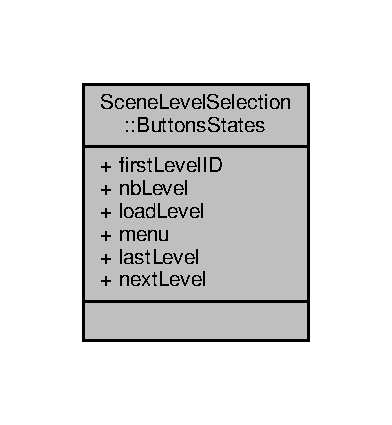
\includegraphics[width=188pt]{struct_scene_level_selection_1_1_buttons_states__coll__graph}
\end{center}
\end{figure}
\subsection*{Public Attributes}
\begin{DoxyCompactItemize}
\item 
uint32\+\_\+t \hyperlink{struct_scene_level_selection_1_1_buttons_states_ad5dae3335f66dd93bd65153cd7465f4e}{first\+Level\+ID}
\item 
uint32\+\_\+t \hyperlink{struct_scene_level_selection_1_1_buttons_states_a0a628ace7937488fc961b18ce23cd622}{nb\+Level}
\item 
bool \hyperlink{struct_scene_level_selection_1_1_buttons_states_aab6f53d5523d24d763220bff9145dd6b}{load\+Level}
\item 
bool \hyperlink{struct_scene_level_selection_1_1_buttons_states_a57363bd7554b83d2233b457c71101aae}{menu}
\item 
bool \hyperlink{struct_scene_level_selection_1_1_buttons_states_acf37f26590be528e2fffe7b028170660}{last\+Level}
\item 
bool \hyperlink{struct_scene_level_selection_1_1_buttons_states_a9f5d5504cea6bb40837ec15734e712b1}{next\+Level}
\end{DoxyCompactItemize}


\subsection{Detailed Description}
All buttons states. 

\subsection{Member Data Documentation}
\mbox{\Hypertarget{struct_scene_level_selection_1_1_buttons_states_ad5dae3335f66dd93bd65153cd7465f4e}\label{struct_scene_level_selection_1_1_buttons_states_ad5dae3335f66dd93bd65153cd7465f4e}} 
\index{Scene\+Level\+Selection\+::\+Buttons\+States@{Scene\+Level\+Selection\+::\+Buttons\+States}!first\+Level\+ID@{first\+Level\+ID}}
\index{first\+Level\+ID@{first\+Level\+ID}!Scene\+Level\+Selection\+::\+Buttons\+States@{Scene\+Level\+Selection\+::\+Buttons\+States}}
\subsubsection{\texorpdfstring{first\+Level\+ID}{firstLevelID}}
{\footnotesize\ttfamily uint32\+\_\+t Scene\+Level\+Selection\+::\+Buttons\+States\+::first\+Level\+ID}

Id of UI for the first level \mbox{\Hypertarget{struct_scene_level_selection_1_1_buttons_states_acf37f26590be528e2fffe7b028170660}\label{struct_scene_level_selection_1_1_buttons_states_acf37f26590be528e2fffe7b028170660}} 
\index{Scene\+Level\+Selection\+::\+Buttons\+States@{Scene\+Level\+Selection\+::\+Buttons\+States}!last\+Level@{last\+Level}}
\index{last\+Level@{last\+Level}!Scene\+Level\+Selection\+::\+Buttons\+States@{Scene\+Level\+Selection\+::\+Buttons\+States}}
\subsubsection{\texorpdfstring{last\+Level}{lastLevel}}
{\footnotesize\ttfamily bool Scene\+Level\+Selection\+::\+Buttons\+States\+::last\+Level}

True if we clicked on the button last\+Level \mbox{\Hypertarget{struct_scene_level_selection_1_1_buttons_states_aab6f53d5523d24d763220bff9145dd6b}\label{struct_scene_level_selection_1_1_buttons_states_aab6f53d5523d24d763220bff9145dd6b}} 
\index{Scene\+Level\+Selection\+::\+Buttons\+States@{Scene\+Level\+Selection\+::\+Buttons\+States}!load\+Level@{load\+Level}}
\index{load\+Level@{load\+Level}!Scene\+Level\+Selection\+::\+Buttons\+States@{Scene\+Level\+Selection\+::\+Buttons\+States}}
\subsubsection{\texorpdfstring{load\+Level}{loadLevel}}
{\footnotesize\ttfamily bool Scene\+Level\+Selection\+::\+Buttons\+States\+::load\+Level}

True if we clicked on the button load\+Level \mbox{\Hypertarget{struct_scene_level_selection_1_1_buttons_states_a57363bd7554b83d2233b457c71101aae}\label{struct_scene_level_selection_1_1_buttons_states_a57363bd7554b83d2233b457c71101aae}} 
\index{Scene\+Level\+Selection\+::\+Buttons\+States@{Scene\+Level\+Selection\+::\+Buttons\+States}!menu@{menu}}
\index{menu@{menu}!Scene\+Level\+Selection\+::\+Buttons\+States@{Scene\+Level\+Selection\+::\+Buttons\+States}}
\subsubsection{\texorpdfstring{menu}{menu}}
{\footnotesize\ttfamily bool Scene\+Level\+Selection\+::\+Buttons\+States\+::menu}

True if we clicked on the button menu \mbox{\Hypertarget{struct_scene_level_selection_1_1_buttons_states_a0a628ace7937488fc961b18ce23cd622}\label{struct_scene_level_selection_1_1_buttons_states_a0a628ace7937488fc961b18ce23cd622}} 
\index{Scene\+Level\+Selection\+::\+Buttons\+States@{Scene\+Level\+Selection\+::\+Buttons\+States}!nb\+Level@{nb\+Level}}
\index{nb\+Level@{nb\+Level}!Scene\+Level\+Selection\+::\+Buttons\+States@{Scene\+Level\+Selection\+::\+Buttons\+States}}
\subsubsection{\texorpdfstring{nb\+Level}{nbLevel}}
{\footnotesize\ttfamily uint32\+\_\+t Scene\+Level\+Selection\+::\+Buttons\+States\+::nb\+Level}

Number of levels \mbox{\Hypertarget{struct_scene_level_selection_1_1_buttons_states_a9f5d5504cea6bb40837ec15734e712b1}\label{struct_scene_level_selection_1_1_buttons_states_a9f5d5504cea6bb40837ec15734e712b1}} 
\index{Scene\+Level\+Selection\+::\+Buttons\+States@{Scene\+Level\+Selection\+::\+Buttons\+States}!next\+Level@{next\+Level}}
\index{next\+Level@{next\+Level}!Scene\+Level\+Selection\+::\+Buttons\+States@{Scene\+Level\+Selection\+::\+Buttons\+States}}
\subsubsection{\texorpdfstring{next\+Level}{nextLevel}}
{\footnotesize\ttfamily bool Scene\+Level\+Selection\+::\+Buttons\+States\+::next\+Level}

True if we clicked on the button next\+Level 

The documentation for this struct was generated from the following file\+:\begin{DoxyCompactItemize}
\item 
includes/scenes/Scene\+Level\+Selection.\+hpp\end{DoxyCompactItemize}

\hypertarget{struct_scene_load_game_1_1_buttons_states}{}\doxysection{Scene\+Load\+Game\+::Buttons\+States Struct Reference}
\label{struct_scene_load_game_1_1_buttons_states}\index{SceneLoadGame::ButtonsStates@{SceneLoadGame::ButtonsStates}}


Collaboration diagram for Scene\+Load\+Game\+::Buttons\+States\+:\nopagebreak
\begin{figure}[H]
\begin{center}
\leavevmode
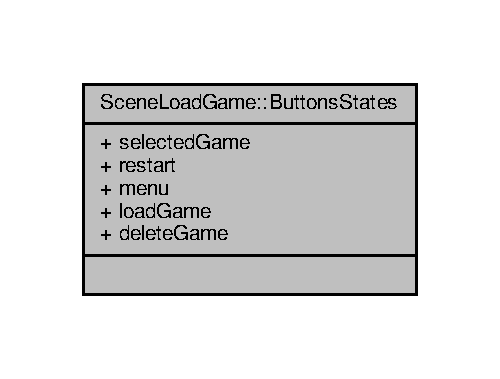
\includegraphics[width=240pt]{struct_scene_load_game_1_1_buttons_states__coll__graph}
\end{center}
\end{figure}
\doxysubsection*{Public Attributes}
\begin{DoxyCompactItemize}
\item 
\mbox{\Hypertarget{struct_scene_load_game_1_1_buttons_states_a23e5e1bfc6c0fcd8362501554db4c015}\label{struct_scene_load_game_1_1_buttons_states_a23e5e1bfc6c0fcd8362501554db4c015}} 
int64\+\_\+t {\bfseries selected\+Game}
\item 
\mbox{\Hypertarget{struct_scene_load_game_1_1_buttons_states_a22a840d0d58839802816cce823f034a3}\label{struct_scene_load_game_1_1_buttons_states_a22a840d0d58839802816cce823f034a3}} 
bool {\bfseries restart}
\item 
\mbox{\Hypertarget{struct_scene_load_game_1_1_buttons_states_a366264c459d2d427b8386b0205ee09e5}\label{struct_scene_load_game_1_1_buttons_states_a366264c459d2d427b8386b0205ee09e5}} 
bool {\bfseries menu}
\item 
\mbox{\Hypertarget{struct_scene_load_game_1_1_buttons_states_a2acccb098559eaea7fc90e5f4c3864f1}\label{struct_scene_load_game_1_1_buttons_states_a2acccb098559eaea7fc90e5f4c3864f1}} 
bool {\bfseries load\+Game}
\item 
\mbox{\Hypertarget{struct_scene_load_game_1_1_buttons_states_a6f2f36945d5e55ad28a2a6196751da90}\label{struct_scene_load_game_1_1_buttons_states_a6f2f36945d5e55ad28a2a6196751da90}} 
bool {\bfseries delete\+Game}
\end{DoxyCompactItemize}


The documentation for this struct was generated from the following file\+:\begin{DoxyCompactItemize}
\item 
includes/scenes/Scene\+Load\+Game.\+hpp\end{DoxyCompactItemize}

\hypertarget{struct_scene_main_menu_1_1_buttons_states}{}\doxysection{Scene\+Main\+Menu\+::Buttons\+States Struct Reference}
\label{struct_scene_main_menu_1_1_buttons_states}\index{SceneMainMenu::ButtonsStates@{SceneMainMenu::ButtonsStates}}


All buttons states.  




{\ttfamily \#include $<$Scene\+Main\+Menu.\+hpp$>$}



Collaboration diagram for Scene\+Main\+Menu\+::Buttons\+States\+:\nopagebreak
\begin{figure}[H]
\begin{center}
\leavevmode
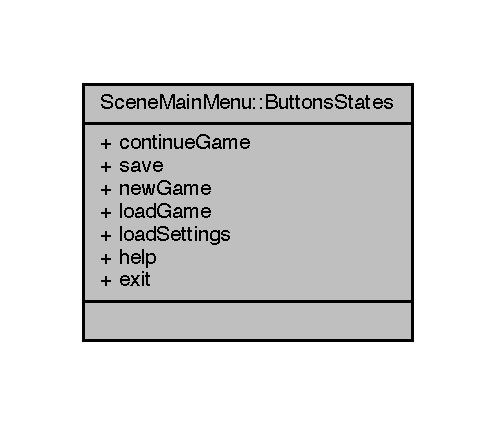
\includegraphics[width=238pt]{struct_scene_main_menu_1_1_buttons_states__coll__graph}
\end{center}
\end{figure}
\doxysubsection*{Public Attributes}
\begin{DoxyCompactItemize}
\item 
bool \mbox{\hyperlink{struct_scene_main_menu_1_1_buttons_states_a134d9fa7b44590be628cfd76661d0328}{continue\+Game}}
\item 
bool \mbox{\hyperlink{struct_scene_main_menu_1_1_buttons_states_aeb015a3f6ff49aa321e9ed50291a0897}{save}}
\item 
bool \mbox{\hyperlink{struct_scene_main_menu_1_1_buttons_states_a266bd47715dbc95ee9b7325327ae1981}{new\+Game}}
\item 
bool \mbox{\hyperlink{struct_scene_main_menu_1_1_buttons_states_a7cce9e898d97a704bd4e4e9e0e243c8c}{load\+Game}}
\item 
bool \mbox{\hyperlink{struct_scene_main_menu_1_1_buttons_states_afcdb7f4b98f2b0166775503a5c69dd8e}{load\+Settings}}
\item 
bool \mbox{\hyperlink{struct_scene_main_menu_1_1_buttons_states_ac927874c333c653cea1458bce713c323}{help}}
\item 
bool \mbox{\hyperlink{struct_scene_main_menu_1_1_buttons_states_ab6cce0f83b5ceb8eee57f57c83e5c744}{exit}}
\end{DoxyCompactItemize}


\doxysubsection{Detailed Description}
All buttons states. 

\doxysubsection{Member Data Documentation}
\mbox{\Hypertarget{struct_scene_main_menu_1_1_buttons_states_a134d9fa7b44590be628cfd76661d0328}\label{struct_scene_main_menu_1_1_buttons_states_a134d9fa7b44590be628cfd76661d0328}} 
\index{SceneMainMenu::ButtonsStates@{SceneMainMenu::ButtonsStates}!continueGame@{continueGame}}
\index{continueGame@{continueGame}!SceneMainMenu::ButtonsStates@{SceneMainMenu::ButtonsStates}}
\doxysubsubsection{\texorpdfstring{continueGame}{continueGame}}
{\footnotesize\ttfamily bool Scene\+Main\+Menu\+::\+Buttons\+States\+::continue\+Game}

True if we clicked on the button continue\+Game \mbox{\Hypertarget{struct_scene_main_menu_1_1_buttons_states_ab6cce0f83b5ceb8eee57f57c83e5c744}\label{struct_scene_main_menu_1_1_buttons_states_ab6cce0f83b5ceb8eee57f57c83e5c744}} 
\index{SceneMainMenu::ButtonsStates@{SceneMainMenu::ButtonsStates}!exit@{exit}}
\index{exit@{exit}!SceneMainMenu::ButtonsStates@{SceneMainMenu::ButtonsStates}}
\doxysubsubsection{\texorpdfstring{exit}{exit}}
{\footnotesize\ttfamily bool Scene\+Main\+Menu\+::\+Buttons\+States\+::exit}

True if we clicked on the button exit \mbox{\Hypertarget{struct_scene_main_menu_1_1_buttons_states_ac927874c333c653cea1458bce713c323}\label{struct_scene_main_menu_1_1_buttons_states_ac927874c333c653cea1458bce713c323}} 
\index{SceneMainMenu::ButtonsStates@{SceneMainMenu::ButtonsStates}!help@{help}}
\index{help@{help}!SceneMainMenu::ButtonsStates@{SceneMainMenu::ButtonsStates}}
\doxysubsubsection{\texorpdfstring{help}{help}}
{\footnotesize\ttfamily bool Scene\+Main\+Menu\+::\+Buttons\+States\+::help}

True if we clicked on the help button \mbox{\Hypertarget{struct_scene_main_menu_1_1_buttons_states_a7cce9e898d97a704bd4e4e9e0e243c8c}\label{struct_scene_main_menu_1_1_buttons_states_a7cce9e898d97a704bd4e4e9e0e243c8c}} 
\index{SceneMainMenu::ButtonsStates@{SceneMainMenu::ButtonsStates}!loadGame@{loadGame}}
\index{loadGame@{loadGame}!SceneMainMenu::ButtonsStates@{SceneMainMenu::ButtonsStates}}
\doxysubsubsection{\texorpdfstring{loadGame}{loadGame}}
{\footnotesize\ttfamily bool Scene\+Main\+Menu\+::\+Buttons\+States\+::load\+Game}

True if we clicked on the button load\+Game \mbox{\Hypertarget{struct_scene_main_menu_1_1_buttons_states_afcdb7f4b98f2b0166775503a5c69dd8e}\label{struct_scene_main_menu_1_1_buttons_states_afcdb7f4b98f2b0166775503a5c69dd8e}} 
\index{SceneMainMenu::ButtonsStates@{SceneMainMenu::ButtonsStates}!loadSettings@{loadSettings}}
\index{loadSettings@{loadSettings}!SceneMainMenu::ButtonsStates@{SceneMainMenu::ButtonsStates}}
\doxysubsubsection{\texorpdfstring{loadSettings}{loadSettings}}
{\footnotesize\ttfamily bool Scene\+Main\+Menu\+::\+Buttons\+States\+::load\+Settings}

True if we clicked on the button load\+Settings \mbox{\Hypertarget{struct_scene_main_menu_1_1_buttons_states_a266bd47715dbc95ee9b7325327ae1981}\label{struct_scene_main_menu_1_1_buttons_states_a266bd47715dbc95ee9b7325327ae1981}} 
\index{SceneMainMenu::ButtonsStates@{SceneMainMenu::ButtonsStates}!newGame@{newGame}}
\index{newGame@{newGame}!SceneMainMenu::ButtonsStates@{SceneMainMenu::ButtonsStates}}
\doxysubsubsection{\texorpdfstring{newGame}{newGame}}
{\footnotesize\ttfamily bool Scene\+Main\+Menu\+::\+Buttons\+States\+::new\+Game}

True if we clicked on the button new\+Game \mbox{\Hypertarget{struct_scene_main_menu_1_1_buttons_states_aeb015a3f6ff49aa321e9ed50291a0897}\label{struct_scene_main_menu_1_1_buttons_states_aeb015a3f6ff49aa321e9ed50291a0897}} 
\index{SceneMainMenu::ButtonsStates@{SceneMainMenu::ButtonsStates}!save@{save}}
\index{save@{save}!SceneMainMenu::ButtonsStates@{SceneMainMenu::ButtonsStates}}
\doxysubsubsection{\texorpdfstring{save}{save}}
{\footnotesize\ttfamily bool Scene\+Main\+Menu\+::\+Buttons\+States\+::save}

True if we clicked on the button save 

The documentation for this struct was generated from the following file\+:\begin{DoxyCompactItemize}
\item 
includes/scenes/Scene\+Main\+Menu.\+hpp\end{DoxyCompactItemize}

\hypertarget{struct_scene_pause_1_1_buttons_states}{}\section{Scene\+Pause\+:\+:Buttons\+States Struct Reference}
\label{struct_scene_pause_1_1_buttons_states}\index{Scene\+Pause\+::\+Buttons\+States@{Scene\+Pause\+::\+Buttons\+States}}


All buttons states.  




{\ttfamily \#include $<$Scene\+Pause.\+hpp$>$}



Collaboration diagram for Scene\+Pause\+:\+:Buttons\+States\+:
\nopagebreak
\begin{figure}[H]
\begin{center}
\leavevmode
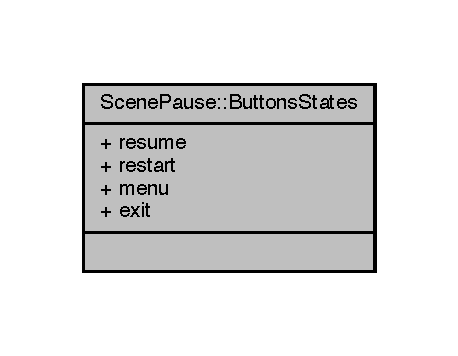
\includegraphics[width=220pt]{struct_scene_pause_1_1_buttons_states__coll__graph}
\end{center}
\end{figure}
\subsection*{Public Attributes}
\begin{DoxyCompactItemize}
\item 
bool \hyperlink{struct_scene_pause_1_1_buttons_states_a59b513318486097a19f02f4028aa3fe8}{resume}
\item 
bool \hyperlink{struct_scene_pause_1_1_buttons_states_a34df4897a0189b1e07f2ac4391081e62}{restart}
\item 
bool \hyperlink{struct_scene_pause_1_1_buttons_states_aa61a79ff606be18223d834445c08ea8e}{help}
\item 
bool \hyperlink{struct_scene_pause_1_1_buttons_states_a507c26169d7ecbe5bd048790044c5e21}{menu}
\item 
bool \hyperlink{struct_scene_pause_1_1_buttons_states_af36a05e31bbdb2c9bfc29b81ea196d2f}{exit}
\end{DoxyCompactItemize}


\subsection{Detailed Description}
All buttons states. 

\subsection{Member Data Documentation}
\mbox{\Hypertarget{struct_scene_pause_1_1_buttons_states_af36a05e31bbdb2c9bfc29b81ea196d2f}\label{struct_scene_pause_1_1_buttons_states_af36a05e31bbdb2c9bfc29b81ea196d2f}} 
\index{Scene\+Pause\+::\+Buttons\+States@{Scene\+Pause\+::\+Buttons\+States}!exit@{exit}}
\index{exit@{exit}!Scene\+Pause\+::\+Buttons\+States@{Scene\+Pause\+::\+Buttons\+States}}
\subsubsection{\texorpdfstring{exit}{exit}}
{\footnotesize\ttfamily bool Scene\+Pause\+::\+Buttons\+States\+::exit}

True if we clicked on the button exit \mbox{\Hypertarget{struct_scene_pause_1_1_buttons_states_aa61a79ff606be18223d834445c08ea8e}\label{struct_scene_pause_1_1_buttons_states_aa61a79ff606be18223d834445c08ea8e}} 
\index{Scene\+Pause\+::\+Buttons\+States@{Scene\+Pause\+::\+Buttons\+States}!help@{help}}
\index{help@{help}!Scene\+Pause\+::\+Buttons\+States@{Scene\+Pause\+::\+Buttons\+States}}
\subsubsection{\texorpdfstring{help}{help}}
{\footnotesize\ttfamily bool Scene\+Pause\+::\+Buttons\+States\+::help}

True if we clicked on the button help \mbox{\Hypertarget{struct_scene_pause_1_1_buttons_states_a507c26169d7ecbe5bd048790044c5e21}\label{struct_scene_pause_1_1_buttons_states_a507c26169d7ecbe5bd048790044c5e21}} 
\index{Scene\+Pause\+::\+Buttons\+States@{Scene\+Pause\+::\+Buttons\+States}!menu@{menu}}
\index{menu@{menu}!Scene\+Pause\+::\+Buttons\+States@{Scene\+Pause\+::\+Buttons\+States}}
\subsubsection{\texorpdfstring{menu}{menu}}
{\footnotesize\ttfamily bool Scene\+Pause\+::\+Buttons\+States\+::menu}

True if we clicked on the button menu \mbox{\Hypertarget{struct_scene_pause_1_1_buttons_states_a34df4897a0189b1e07f2ac4391081e62}\label{struct_scene_pause_1_1_buttons_states_a34df4897a0189b1e07f2ac4391081e62}} 
\index{Scene\+Pause\+::\+Buttons\+States@{Scene\+Pause\+::\+Buttons\+States}!restart@{restart}}
\index{restart@{restart}!Scene\+Pause\+::\+Buttons\+States@{Scene\+Pause\+::\+Buttons\+States}}
\subsubsection{\texorpdfstring{restart}{restart}}
{\footnotesize\ttfamily bool Scene\+Pause\+::\+Buttons\+States\+::restart}

True if we clicked on the button restart \mbox{\Hypertarget{struct_scene_pause_1_1_buttons_states_a59b513318486097a19f02f4028aa3fe8}\label{struct_scene_pause_1_1_buttons_states_a59b513318486097a19f02f4028aa3fe8}} 
\index{Scene\+Pause\+::\+Buttons\+States@{Scene\+Pause\+::\+Buttons\+States}!resume@{resume}}
\index{resume@{resume}!Scene\+Pause\+::\+Buttons\+States@{Scene\+Pause\+::\+Buttons\+States}}
\subsubsection{\texorpdfstring{resume}{resume}}
{\footnotesize\ttfamily bool Scene\+Pause\+::\+Buttons\+States\+::resume}

True if we clicked on the button resume 

The documentation for this struct was generated from the following file\+:\begin{DoxyCompactItemize}
\item 
includes/scenes/Scene\+Pause.\+hpp\end{DoxyCompactItemize}

\hypertarget{struct_scene_victory_1_1_buttons_states}{}\section{Scene\+Victory\+:\+:Buttons\+States Struct Reference}
\label{struct_scene_victory_1_1_buttons_states}\index{Scene\+Victory\+::\+Buttons\+States@{Scene\+Victory\+::\+Buttons\+States}}


All buttons states.  




{\ttfamily \#include $<$Scene\+Victory.\+hpp$>$}



Collaboration diagram for Scene\+Victory\+:\+:Buttons\+States\+:
\nopagebreak
\begin{figure}[H]
\begin{center}
\leavevmode
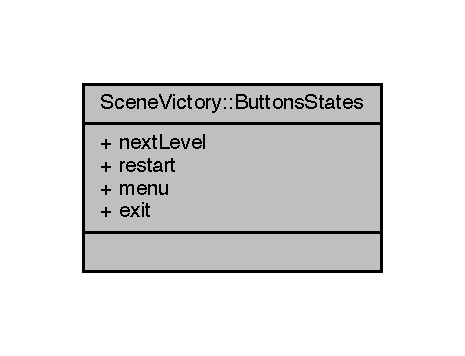
\includegraphics[width=223pt]{struct_scene_victory_1_1_buttons_states__coll__graph}
\end{center}
\end{figure}
\subsection*{Public Attributes}
\begin{DoxyCompactItemize}
\item 
bool \hyperlink{struct_scene_victory_1_1_buttons_states_a6e8b4b9bd0621f109f5f82e9be2b821f}{next\+Level}
\item 
bool \hyperlink{struct_scene_victory_1_1_buttons_states_af0bcebde97f25cd4ea16141b88d55017}{restart}
\item 
bool \hyperlink{struct_scene_victory_1_1_buttons_states_ab39d304bde68866c2356b3535fe2c189}{menu}
\item 
bool \hyperlink{struct_scene_victory_1_1_buttons_states_ae21b1f2a07cc2dc9969a067ecfdf2fff}{exit}
\end{DoxyCompactItemize}


\subsection{Detailed Description}
All buttons states. 

\subsection{Member Data Documentation}
\mbox{\Hypertarget{struct_scene_victory_1_1_buttons_states_ae21b1f2a07cc2dc9969a067ecfdf2fff}\label{struct_scene_victory_1_1_buttons_states_ae21b1f2a07cc2dc9969a067ecfdf2fff}} 
\index{Scene\+Victory\+::\+Buttons\+States@{Scene\+Victory\+::\+Buttons\+States}!exit@{exit}}
\index{exit@{exit}!Scene\+Victory\+::\+Buttons\+States@{Scene\+Victory\+::\+Buttons\+States}}
\subsubsection{\texorpdfstring{exit}{exit}}
{\footnotesize\ttfamily bool Scene\+Victory\+::\+Buttons\+States\+::exit}

True if we clicked on the button exit \mbox{\Hypertarget{struct_scene_victory_1_1_buttons_states_ab39d304bde68866c2356b3535fe2c189}\label{struct_scene_victory_1_1_buttons_states_ab39d304bde68866c2356b3535fe2c189}} 
\index{Scene\+Victory\+::\+Buttons\+States@{Scene\+Victory\+::\+Buttons\+States}!menu@{menu}}
\index{menu@{menu}!Scene\+Victory\+::\+Buttons\+States@{Scene\+Victory\+::\+Buttons\+States}}
\subsubsection{\texorpdfstring{menu}{menu}}
{\footnotesize\ttfamily bool Scene\+Victory\+::\+Buttons\+States\+::menu}

True if we clicked on the button menu \mbox{\Hypertarget{struct_scene_victory_1_1_buttons_states_a6e8b4b9bd0621f109f5f82e9be2b821f}\label{struct_scene_victory_1_1_buttons_states_a6e8b4b9bd0621f109f5f82e9be2b821f}} 
\index{Scene\+Victory\+::\+Buttons\+States@{Scene\+Victory\+::\+Buttons\+States}!next\+Level@{next\+Level}}
\index{next\+Level@{next\+Level}!Scene\+Victory\+::\+Buttons\+States@{Scene\+Victory\+::\+Buttons\+States}}
\subsubsection{\texorpdfstring{next\+Level}{nextLevel}}
{\footnotesize\ttfamily bool Scene\+Victory\+::\+Buttons\+States\+::next\+Level}

True if we clicked on the button next\+Level \mbox{\Hypertarget{struct_scene_victory_1_1_buttons_states_af0bcebde97f25cd4ea16141b88d55017}\label{struct_scene_victory_1_1_buttons_states_af0bcebde97f25cd4ea16141b88d55017}} 
\index{Scene\+Victory\+::\+Buttons\+States@{Scene\+Victory\+::\+Buttons\+States}!restart@{restart}}
\index{restart@{restart}!Scene\+Victory\+::\+Buttons\+States@{Scene\+Victory\+::\+Buttons\+States}}
\subsubsection{\texorpdfstring{restart}{restart}}
{\footnotesize\ttfamily bool Scene\+Victory\+::\+Buttons\+States\+::restart}

True if we clicked on the button restart 

The documentation for this struct was generated from the following file\+:\begin{DoxyCompactItemize}
\item 
includes/scenes/Scene\+Victory.\+hpp\end{DoxyCompactItemize}

\hypertarget{struct_scene_difficulty_1_1_buttons_states}{}\doxysection{Scene\+Difficulty\+::Buttons\+States Struct Reference}
\label{struct_scene_difficulty_1_1_buttons_states}\index{SceneDifficulty::ButtonsStates@{SceneDifficulty::ButtonsStates}}


All buttons states.  




{\ttfamily \#include $<$Scene\+Difficulty.\+hpp$>$}



Collaboration diagram for Scene\+Difficulty\+::Buttons\+States\+:\nopagebreak
\begin{figure}[H]
\begin{center}
\leavevmode
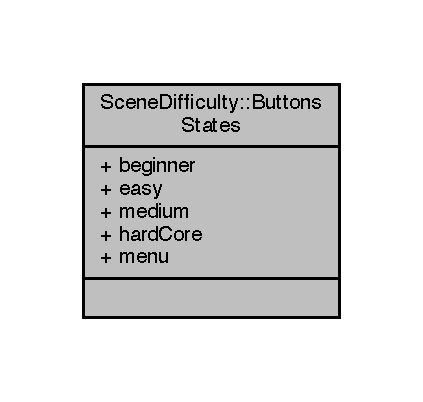
\includegraphics[width=203pt]{struct_scene_difficulty_1_1_buttons_states__coll__graph}
\end{center}
\end{figure}
\doxysubsection*{Public Attributes}
\begin{DoxyCompactItemize}
\item 
bool \mbox{\hyperlink{struct_scene_difficulty_1_1_buttons_states_a8290e8e55a7a4b9f9e16bb6d26d04094}{beginner}}
\item 
bool \mbox{\hyperlink{struct_scene_difficulty_1_1_buttons_states_abf5024bace9449638735654ffc3393fa}{easy}}
\item 
bool \mbox{\hyperlink{struct_scene_difficulty_1_1_buttons_states_a65a48af3d63e00b03e32802d7225394e}{medium}}
\item 
bool \mbox{\hyperlink{struct_scene_difficulty_1_1_buttons_states_ad55ca523d47750a99e15949e56c8afa6}{hard\+Core}}
\item 
bool \mbox{\hyperlink{struct_scene_difficulty_1_1_buttons_states_a407725512ff211f083177c2ea3e4c26f}{menu}}
\end{DoxyCompactItemize}


\doxysubsection{Detailed Description}
All buttons states. 

\doxysubsection{Member Data Documentation}
\mbox{\Hypertarget{struct_scene_difficulty_1_1_buttons_states_a8290e8e55a7a4b9f9e16bb6d26d04094}\label{struct_scene_difficulty_1_1_buttons_states_a8290e8e55a7a4b9f9e16bb6d26d04094}} 
\index{SceneDifficulty::ButtonsStates@{SceneDifficulty::ButtonsStates}!beginner@{beginner}}
\index{beginner@{beginner}!SceneDifficulty::ButtonsStates@{SceneDifficulty::ButtonsStates}}
\doxysubsubsection{\texorpdfstring{beginner}{beginner}}
{\footnotesize\ttfamily bool Scene\+Difficulty\+::\+Buttons\+States\+::beginner}

True if we clicked on the button beginner \mbox{\Hypertarget{struct_scene_difficulty_1_1_buttons_states_abf5024bace9449638735654ffc3393fa}\label{struct_scene_difficulty_1_1_buttons_states_abf5024bace9449638735654ffc3393fa}} 
\index{SceneDifficulty::ButtonsStates@{SceneDifficulty::ButtonsStates}!easy@{easy}}
\index{easy@{easy}!SceneDifficulty::ButtonsStates@{SceneDifficulty::ButtonsStates}}
\doxysubsubsection{\texorpdfstring{easy}{easy}}
{\footnotesize\ttfamily bool Scene\+Difficulty\+::\+Buttons\+States\+::easy}

True if we clicked on the button easy \mbox{\Hypertarget{struct_scene_difficulty_1_1_buttons_states_ad55ca523d47750a99e15949e56c8afa6}\label{struct_scene_difficulty_1_1_buttons_states_ad55ca523d47750a99e15949e56c8afa6}} 
\index{SceneDifficulty::ButtonsStates@{SceneDifficulty::ButtonsStates}!hardCore@{hardCore}}
\index{hardCore@{hardCore}!SceneDifficulty::ButtonsStates@{SceneDifficulty::ButtonsStates}}
\doxysubsubsection{\texorpdfstring{hardCore}{hardCore}}
{\footnotesize\ttfamily bool Scene\+Difficulty\+::\+Buttons\+States\+::hard\+Core}

True if we clicked on the button hard\+Core \mbox{\Hypertarget{struct_scene_difficulty_1_1_buttons_states_a65a48af3d63e00b03e32802d7225394e}\label{struct_scene_difficulty_1_1_buttons_states_a65a48af3d63e00b03e32802d7225394e}} 
\index{SceneDifficulty::ButtonsStates@{SceneDifficulty::ButtonsStates}!medium@{medium}}
\index{medium@{medium}!SceneDifficulty::ButtonsStates@{SceneDifficulty::ButtonsStates}}
\doxysubsubsection{\texorpdfstring{medium}{medium}}
{\footnotesize\ttfamily bool Scene\+Difficulty\+::\+Buttons\+States\+::medium}

True if we clicked on the button medium \mbox{\Hypertarget{struct_scene_difficulty_1_1_buttons_states_a407725512ff211f083177c2ea3e4c26f}\label{struct_scene_difficulty_1_1_buttons_states_a407725512ff211f083177c2ea3e4c26f}} 
\index{SceneDifficulty::ButtonsStates@{SceneDifficulty::ButtonsStates}!menu@{menu}}
\index{menu@{menu}!SceneDifficulty::ButtonsStates@{SceneDifficulty::ButtonsStates}}
\doxysubsubsection{\texorpdfstring{menu}{menu}}
{\footnotesize\ttfamily bool Scene\+Difficulty\+::\+Buttons\+States\+::menu}

True if we clicked on the menu button 

The documentation for this struct was generated from the following file\+:\begin{DoxyCompactItemize}
\item 
includes/scenes/Scene\+Difficulty.\+hpp\end{DoxyCompactItemize}

\hypertarget{class_button_u_i}{}\section{Button\+UI Class Reference}
\label{class_button_u_i}\index{Button\+UI@{Button\+UI}}


this is the UI for button  




{\ttfamily \#include $<$Button\+U\+I.\+hpp$>$}



Inheritance diagram for Button\+UI\+:
\nopagebreak
\begin{figure}[H]
\begin{center}
\leavevmode
\includegraphics[height=550pt]{class_button_u_i__inherit__graph}
\end{center}
\end{figure}


Collaboration diagram for Button\+UI\+:
\nopagebreak
\begin{figure}[H]
\begin{center}
\leavevmode
\includegraphics[height=550pt]{class_button_u_i__coll__graph}
\end{center}
\end{figure}
\subsection*{Public Member Functions}
\begin{DoxyCompactItemize}
\item 
\hyperlink{class_button_u_i_a06e5f10c62feee5baf35f88f3af574b2}{Button\+UI} (glm\+::vec2 pos, glm\+::vec2 size)
\begin{DoxyCompactList}\small\item\em Construct a new Button U I\+:\+: Button U I object. \end{DoxyCompactList}\item 
\hyperlink{class_button_u_i_a64d56901e494b8ae4fdd550631135ce0}{Button\+UI} (\hyperlink{class_button_u_i}{Button\+UI} const \&src)
\begin{DoxyCompactList}\small\item\em Construct a new Button U I\+:\+: Button U I object. \end{DoxyCompactList}\item 
\mbox{\Hypertarget{class_button_u_i_aec36b3db802067fa7a2f4bf0d7104284}\label{class_button_u_i_aec36b3db802067fa7a2f4bf0d7104284}} 
virtual \hyperlink{class_button_u_i_aec36b3db802067fa7a2f4bf0d7104284}{$\sim$\+Button\+UI} ()
\begin{DoxyCompactList}\small\item\em Destroy the Button U I\+:\+: Button U I object. \end{DoxyCompactList}\item 
\hyperlink{class_button_u_i}{Button\+UI} \& \hyperlink{class_button_u_i_a17cfc6a63fb650c756d7f0afadad665e}{operator=} (\hyperlink{class_button_u_i}{Button\+UI} const \&rhs)
\begin{DoxyCompactList}\small\item\em Copy this object. \end{DoxyCompactList}\end{DoxyCompactItemize}
\subsection*{Protected Member Functions}
\begin{DoxyCompactItemize}
\item 
\mbox{\Hypertarget{class_button_u_i_a984a9fd2a19550a1a39a7ab905fe1f14}\label{class_button_u_i_a984a9fd2a19550a1a39a7ab905fe1f14}} 
virtual void \hyperlink{class_button_u_i_a984a9fd2a19550a1a39a7ab905fe1f14}{\+\_\+update} ()
\begin{DoxyCompactList}\small\item\em this is the base update function of UI objects \end{DoxyCompactList}\item 
\mbox{\Hypertarget{class_button_u_i_aa183e89b7efbc8eed5fc91ce16029725}\label{class_button_u_i_aa183e89b7efbc8eed5fc91ce16029725}} 
virtual void \hyperlink{class_button_u_i_aa183e89b7efbc8eed5fc91ce16029725}{\+\_\+draw} ()
\begin{DoxyCompactList}\small\item\em this is the draw function for UI /!\textbackslash{} -\/$>$ you need to draw in the reverse order (draw at first the element on the top) \end{DoxyCompactList}\end{DoxyCompactItemize}
\subsection*{Additional Inherited Members}


\subsection{Detailed Description}
this is the UI for button 

\subsection{Constructor \& Destructor Documentation}
\mbox{\Hypertarget{class_button_u_i_a06e5f10c62feee5baf35f88f3af574b2}\label{class_button_u_i_a06e5f10c62feee5baf35f88f3af574b2}} 
\index{Button\+UI@{Button\+UI}!Button\+UI@{Button\+UI}}
\index{Button\+UI@{Button\+UI}!Button\+UI@{Button\+UI}}
\subsubsection{\texorpdfstring{Button\+U\+I()}{ButtonUI()}\hspace{0.1cm}{\footnotesize\ttfamily [1/2]}}
{\footnotesize\ttfamily Button\+U\+I\+::\+Button\+UI (\begin{DoxyParamCaption}\item[{glm\+::vec2}]{pos,  }\item[{glm\+::vec2}]{size }\end{DoxyParamCaption})}



Construct a new Button U I\+:\+: Button U I object. 


\begin{DoxyParams}{Parameters}
{\em pos} & The position of the UI element \\
\hline
{\em size} & The size of the UI element \\
\hline
\end{DoxyParams}
\mbox{\Hypertarget{class_button_u_i_a64d56901e494b8ae4fdd550631135ce0}\label{class_button_u_i_a64d56901e494b8ae4fdd550631135ce0}} 
\index{Button\+UI@{Button\+UI}!Button\+UI@{Button\+UI}}
\index{Button\+UI@{Button\+UI}!Button\+UI@{Button\+UI}}
\subsubsection{\texorpdfstring{Button\+U\+I()}{ButtonUI()}\hspace{0.1cm}{\footnotesize\ttfamily [2/2]}}
{\footnotesize\ttfamily Button\+U\+I\+::\+Button\+UI (\begin{DoxyParamCaption}\item[{\hyperlink{class_button_u_i}{Button\+UI} const \&}]{src }\end{DoxyParamCaption})}



Construct a new Button U I\+:\+: Button U I object. 


\begin{DoxyParams}{Parameters}
{\em src} & The object to do the copy \\
\hline
\end{DoxyParams}


\subsection{Member Function Documentation}
\mbox{\Hypertarget{class_button_u_i_a17cfc6a63fb650c756d7f0afadad665e}\label{class_button_u_i_a17cfc6a63fb650c756d7f0afadad665e}} 
\index{Button\+UI@{Button\+UI}!operator=@{operator=}}
\index{operator=@{operator=}!Button\+UI@{Button\+UI}}
\subsubsection{\texorpdfstring{operator=()}{operator=()}}
{\footnotesize\ttfamily \hyperlink{class_button_u_i}{Button\+UI} \& Button\+U\+I\+::operator= (\begin{DoxyParamCaption}\item[{\hyperlink{class_button_u_i}{Button\+UI} const \&}]{rhs }\end{DoxyParamCaption})}



Copy this object. 


\begin{DoxyParams}{Parameters}
{\em rhs} & The object to copy \\
\hline
\end{DoxyParams}
\begin{DoxyReturn}{Returns}
\hyperlink{class_button_u_i}{Button\+UI}\& A reference to the copied object 
\end{DoxyReturn}


The documentation for this class was generated from the following files\+:\begin{DoxyCompactItemize}
\item 
includes/utils/opengl/\+U\+I/Button\+U\+I.\+hpp\item 
srcs/utils/opengl/\+U\+I/Button\+U\+I.\+cpp\end{DoxyCompactItemize}

\hypertarget{class_camera}{}\doxysection{Camera Class Reference}
\label{class_camera}\index{Camera@{Camera}}


this is a camera 3D object  




{\ttfamily \#include $<$Camera.\+hpp$>$}



Collaboration diagram for Camera\+:
\nopagebreak
\begin{figure}[H]
\begin{center}
\leavevmode
\includegraphics[width=181pt]{class_camera__coll__graph}
\end{center}
\end{figure}
\doxysubsection*{Public Member Functions}
\begin{DoxyCompactItemize}
\item 
\mbox{\Hypertarget{class_camera_a9013f69b8ad8b9f17c23cc9fd4bb25be}\label{class_camera_a9013f69b8ad8b9f17c23cc9fd4bb25be}} 
{\bfseries Camera} (float const ratio, C\+A\+M\+E\+R\+A\+\_\+\+V\+E\+C3 pos=C\+A\+M\+E\+R\+A\+\_\+\+V\+E\+C3(0.\+0f, 0.\+0f, 0.\+0f), C\+A\+M\+E\+R\+A\+\_\+\+V\+E\+C3 up=C\+A\+M\+E\+R\+A\+\_\+\+V\+E\+C3(0.\+0, 1.\+0, 0.\+0), C\+A\+M\+E\+R\+A\+\_\+\+F\+L\+O\+AT yaw=-\/90.\+0f, C\+A\+M\+E\+R\+A\+\_\+\+F\+L\+O\+AT pitch=0.\+0f)
\item 
\mbox{\Hypertarget{class_camera_ae436ecbffdf1bb1117a723603f5b9a63}\label{class_camera_ae436ecbffdf1bb1117a723603f5b9a63}} 
{\bfseries Camera} (\mbox{\hyperlink{class_camera}{Camera}} const \&src)
\item 
\mbox{\Hypertarget{class_camera_a7df2f4b79b58047d59902a2e8b40855d}\label{class_camera_a7df2f4b79b58047d59902a2e8b40855d}} 
\mbox{\hyperlink{class_camera}{Camera}} \& {\bfseries operator=} (\mbox{\hyperlink{class_camera}{Camera}} const \&rhs)
\item 
void \mbox{\hyperlink{class_camera_a54c2f4e2c30c1fc0c82499982b59e6e0}{look\+At}} (C\+A\+M\+E\+R\+A\+\_\+\+V\+E\+C3 target)
\begin{DoxyCompactList}\small\item\em Move the camera orientation to look at the target. \end{DoxyCompactList}\item 
\mbox{\Hypertarget{class_camera_ac59fb0da1e1cb188063ce8cf227d3a2f}\label{class_camera_ac59fb0da1e1cb188063ce8cf227d3a2f}} 
void \mbox{\hyperlink{class_camera_ac59fb0da1e1cb188063ce8cf227d3a2f}{reset\+Position}} ()
\begin{DoxyCompactList}\small\item\em Reset the camera position. \end{DoxyCompactList}\item 
\mbox{\Hypertarget{class_camera_a2ddcff55d196d1c57a3310d9c6119f95}\label{class_camera_a2ddcff55d196d1c57a3310d9c6119f95}} 
void {\bfseries set\+Ratio} (float ratio)
\item 
\mbox{\Hypertarget{class_camera_a3138aa2e40815013739ddb71502ca608}\label{class_camera_a3138aa2e40815013739ddb71502ca608}} 
void {\bfseries set\+FovY} (float fovY)
\item 
\mbox{\Hypertarget{class_camera_afcb04b0f02749e07b61e3346d34834da}\label{class_camera_afcb04b0f02749e07b61e3346d34834da}} 
void {\bfseries set\+Near\+And\+Far} (float near, float far)
\item 
void \mbox{\hyperlink{class_camera_a90617e4799a43f0b74ede1d6caca958e}{set\+Mode}} (Cam\+Mode\+::\+Enum mode)
\begin{DoxyCompactList}\small\item\em Update the current camera mode. \end{DoxyCompactList}\item 
void \mbox{\hyperlink{class_camera_aa83a6e3f89b6a1bdd4578d4cd84fdfde}{set\+Def\+Pos}} (C\+A\+M\+E\+R\+A\+\_\+\+V\+E\+C3 def\+Pos, C\+A\+M\+E\+R\+A\+\_\+\+F\+L\+O\+AT def\+Yaw=-\/90, C\+A\+M\+E\+R\+A\+\_\+\+F\+L\+O\+AT def\+Pitch=0)
\begin{DoxyCompactList}\small\item\em Set the default camera position. \end{DoxyCompactList}\item 
\mbox{\Hypertarget{class_camera_a1e8d069fff363a0d3504714068000654}\label{class_camera_a1e8d069fff363a0d3504714068000654}} 
void \mbox{\hyperlink{class_camera_a1e8d069fff363a0d3504714068000654}{set\+Def\+Pos}} ()
\begin{DoxyCompactList}\small\item\em Set the default camera position to the current position. \end{DoxyCompactList}\item 
void \mbox{\hyperlink{class_camera_ad1272976ffb7a0d535c8977ec063201d}{update}} (float dt\+Time)
\begin{DoxyCompactList}\small\item\em Update function of the camera -\/$>$ to be called every frames. \end{DoxyCompactList}\item 
void \mbox{\hyperlink{class_camera_a1f28b91cb62dd318b5acf27296c99242}{process\+Keyboard}} (Cam\+Movement direction, C\+A\+M\+E\+R\+A\+\_\+\+F\+L\+O\+AT dt\+Time, bool is\+Run=false)
\begin{DoxyCompactList}\small\item\em Move camera from keyboard interaction. \end{DoxyCompactList}\item 
void \mbox{\hyperlink{class_camera_abd790165abfcc82595470328193060de}{process\+Mouse\+Movement}} (glm\+::vec2 offset, bool constrain\+Pitch=true)
\begin{DoxyCompactList}\small\item\em Move the camera from the mouse movements. \end{DoxyCompactList}\item 
void \mbox{\hyperlink{class_camera_a4287af0eacc2cf50765360a8e1b5db74}{frustum\+Culling\+Init}} (C\+A\+M\+E\+R\+A\+\_\+\+F\+L\+O\+AT angle\+Deg, C\+A\+M\+E\+R\+A\+\_\+\+F\+L\+O\+AT ratio, C\+A\+M\+E\+R\+A\+\_\+\+F\+L\+O\+AT nearD, C\+A\+M\+E\+R\+A\+\_\+\+F\+L\+O\+AT farD)
\begin{DoxyCompactList}\small\item\em init the frustum culling (take the same args as projection matrix) \end{DoxyCompactList}\item 
int \mbox{\hyperlink{class_camera_aa7a544e123a54e98509cfc6050869aca}{frustum\+Culling\+Check\+Point}} (C\+A\+M\+E\+R\+A\+\_\+\+V\+E\+C3 const \&point) const
\begin{DoxyCompactList}\small\item\em Check if a point is inside or outside the camera. \end{DoxyCompactList}\item 
int \mbox{\hyperlink{class_camera_a7baca010a22bac712351e4c6adca5acf}{frustum\+Culling\+Check\+Cube}} (C\+A\+M\+E\+R\+A\+\_\+\+V\+E\+C3 const \&start\+Point, C\+A\+M\+E\+R\+A\+\_\+\+V\+E\+C3 const \&size) const
\begin{DoxyCompactList}\small\item\em Check if a cube or rectangle is inside or outside of the camera. \end{DoxyCompactList}\item 
\mbox{\Hypertarget{class_camera_a510c9f3ecf465578002fdd03dadb3f6d}\label{class_camera_a510c9f3ecf465578002fdd03dadb3f6d}} 
void {\bfseries reset\+Follow\+Path} ()
\item 
\mbox{\Hypertarget{class_camera_a340c9687399742b3c9c1dec3f02d9b32}\label{class_camera_a340c9687399742b3c9c1dec3f02d9b32}} 
void {\bfseries set\+Follow\+Path} (std\+::vector$<$ \mbox{\hyperlink{struct_cam_point}{Cam\+Point}} $>$ const \&path)
\item 
\mbox{\Hypertarget{class_camera_a9f190ab490492b811ccc3603b68fe70a}\label{class_camera_a9f190ab490492b811ccc3603b68fe70a}} 
void {\bfseries set\+Follow\+Repeat} (bool repeat)
\item 
\mbox{\Hypertarget{class_camera_a56103a197cc727c1d108f5e503e5c6f4}\label{class_camera_a56103a197cc727c1d108f5e503e5c6f4}} 
void {\bfseries set\+Follow\+Speed} (float speed\+\_\+)
\item 
\mbox{\Hypertarget{class_camera_a3e7c256d5df9a0dd554b845e3ece414e}\label{class_camera_a3e7c256d5df9a0dd554b845e3ece414e}} 
bool {\bfseries is\+Follow\+Finished} () const
\item 
\mbox{\Hypertarget{class_camera_aadea4e3706e4a1405c7b035c60d6d69e}\label{class_camera_aadea4e3706e4a1405c7b035c60d6d69e}} 
bool {\bfseries is\+Follow\+Repeat} () const
\item 
\mbox{\Hypertarget{class_camera_aa2e2289caff32f9ac552f1e5c6c7931f}\label{class_camera_aa2e2289caff32f9ac552f1e5c6c7931f}} 
C\+A\+M\+E\+R\+A\+\_\+\+M\+A\+T4 {\bfseries get\+View\+Matrix} () const
\item 
\mbox{\Hypertarget{class_camera_ab6bf7c26da92eb1806f0787eb35e540c}\label{class_camera_ab6bf7c26da92eb1806f0787eb35e540c}} 
C\+A\+M\+E\+R\+A\+\_\+\+M\+A\+T4 {\bfseries get\+Projection} () const
\item 
\mbox{\Hypertarget{class_camera_ab508959139d8555dce6f444e44fc01ed}\label{class_camera_ab508959139d8555dce6f444e44fc01ed}} 
Cam\+Mode\+::\+Enum {\bfseries get\+Mode} () const
\item 
\mbox{\Hypertarget{class_camera_aae10133175e34f9856c48cdb294279df}\label{class_camera_aae10133175e34f9856c48cdb294279df}} 
C\+A\+M\+E\+R\+A\+\_\+\+V\+E\+C3 {\bfseries get\+Def\+Pos} () const
\end{DoxyCompactItemize}
\doxysubsection*{Public Attributes}
\begin{DoxyCompactItemize}
\item 
\mbox{\Hypertarget{class_camera_a645cd9343d8c0160ce2281111240f9fd}\label{class_camera_a645cd9343d8c0160ce2281111240f9fd}} 
C\+A\+M\+E\+R\+A\+\_\+\+V\+E\+C3 {\bfseries pos}
\item 
\mbox{\Hypertarget{class_camera_ab4e78bcb515de19fbac48e3079dd7ccc}\label{class_camera_ab4e78bcb515de19fbac48e3079dd7ccc}} 
C\+A\+M\+E\+R\+A\+\_\+\+V\+E\+C3 {\bfseries front}
\item 
\mbox{\Hypertarget{class_camera_a02d03a426815c0d64522724fbe2374ca}\label{class_camera_a02d03a426815c0d64522724fbe2374ca}} 
C\+A\+M\+E\+R\+A\+\_\+\+V\+E\+C3 {\bfseries up}
\item 
\mbox{\Hypertarget{class_camera_aa242be0f8ab49b72ec65fcdcec807bb5}\label{class_camera_aa242be0f8ab49b72ec65fcdcec807bb5}} 
C\+A\+M\+E\+R\+A\+\_\+\+V\+E\+C3 {\bfseries right}
\item 
\mbox{\Hypertarget{class_camera_a9088ff173e443938f31ed4b6c0f75756}\label{class_camera_a9088ff173e443938f31ed4b6c0f75756}} 
C\+A\+M\+E\+R\+A\+\_\+\+V\+E\+C3 {\bfseries world\+Up}
\item 
\mbox{\Hypertarget{class_camera_aa11a0643425580b4115bb9b839542891}\label{class_camera_aa11a0643425580b4115bb9b839542891}} 
C\+A\+M\+E\+R\+A\+\_\+\+F\+L\+O\+AT {\bfseries yaw}
\item 
\mbox{\Hypertarget{class_camera_aaaff48d7638a7e3cc7e141f11cc23293}\label{class_camera_aaaff48d7638a7e3cc7e141f11cc23293}} 
C\+A\+M\+E\+R\+A\+\_\+\+F\+L\+O\+AT {\bfseries pitch}
\item 
\mbox{\Hypertarget{class_camera_a2e09cc969e7e7733051df9a0bfe9afa0}\label{class_camera_a2e09cc969e7e7733051df9a0bfe9afa0}} 
C\+A\+M\+E\+R\+A\+\_\+\+F\+L\+O\+AT {\bfseries movement\+Speed}
\item 
\mbox{\Hypertarget{class_camera_a0fd9adbe4484147947bc1f51452edd6f}\label{class_camera_a0fd9adbe4484147947bc1f51452edd6f}} 
C\+A\+M\+E\+R\+A\+\_\+\+F\+L\+O\+AT {\bfseries mouse\+Sensitivity}
\item 
\mbox{\Hypertarget{class_camera_a891d353a14161c6be625f6a52b75375d}\label{class_camera_a891d353a14161c6be625f6a52b75375d}} 
C\+A\+M\+E\+R\+A\+\_\+\+F\+L\+O\+AT {\bfseries run\+Factor}
\end{DoxyCompactItemize}


\doxysubsection{Detailed Description}
this is a camera 3D object 

this object implements functions to\+:
\begin{DoxyItemize}
\item move with keyboard (process\+Keyboard)
\item turn camera with mouse (process\+Mouse\+Movement)
\item look at a point (look\+At)
\item know if a 3D point or a 3D rectangle is inside the camera angle (frustum\+Culling...) 
\end{DoxyItemize}

\doxysubsection{Member Function Documentation}
\mbox{\Hypertarget{class_camera_a7baca010a22bac712351e4c6adca5acf}\label{class_camera_a7baca010a22bac712351e4c6adca5acf}} 
\index{Camera@{Camera}!frustumCullingCheckCube@{frustumCullingCheckCube}}
\index{frustumCullingCheckCube@{frustumCullingCheckCube}!Camera@{Camera}}
\doxysubsubsection{\texorpdfstring{frustumCullingCheckCube()}{frustumCullingCheckCube()}}
{\footnotesize\ttfamily int Camera\+::frustum\+Culling\+Check\+Cube (\begin{DoxyParamCaption}\item[{C\+A\+M\+E\+R\+A\+\_\+\+V\+E\+C3 const \&}]{start\+Point,  }\item[{C\+A\+M\+E\+R\+A\+\_\+\+V\+E\+C3 const \&}]{size }\end{DoxyParamCaption}) const}



Check if a cube or rectangle is inside or outside of the camera. 


\begin{DoxyParams}{Parameters}
{\em start\+Point} & The 0$\vert$0$\vert$0 coordinate of the cube \\
\hline
{\em size} & The scale in X Y and Z of the cube \\
\hline
\end{DoxyParams}
\begin{DoxyReturn}{Returns}
int The point position (F\+R\+C\+L\+\_\+\+I\+N\+S\+I\+DE == is inside) 
\end{DoxyReturn}
\mbox{\Hypertarget{class_camera_aa7a544e123a54e98509cfc6050869aca}\label{class_camera_aa7a544e123a54e98509cfc6050869aca}} 
\index{Camera@{Camera}!frustumCullingCheckPoint@{frustumCullingCheckPoint}}
\index{frustumCullingCheckPoint@{frustumCullingCheckPoint}!Camera@{Camera}}
\doxysubsubsection{\texorpdfstring{frustumCullingCheckPoint()}{frustumCullingCheckPoint()}}
{\footnotesize\ttfamily int Camera\+::frustum\+Culling\+Check\+Point (\begin{DoxyParamCaption}\item[{C\+A\+M\+E\+R\+A\+\_\+\+V\+E\+C3 const \&}]{point }\end{DoxyParamCaption}) const}



Check if a point is inside or outside the camera. 


\begin{DoxyParams}{Parameters}
{\em point} & The 3D point \\
\hline
\end{DoxyParams}
\begin{DoxyReturn}{Returns}
int The point position (F\+R\+C\+L\+\_\+\+I\+N\+S\+I\+DE == is inside) 
\end{DoxyReturn}
\mbox{\Hypertarget{class_camera_a4287af0eacc2cf50765360a8e1b5db74}\label{class_camera_a4287af0eacc2cf50765360a8e1b5db74}} 
\index{Camera@{Camera}!frustumCullingInit@{frustumCullingInit}}
\index{frustumCullingInit@{frustumCullingInit}!Camera@{Camera}}
\doxysubsubsection{\texorpdfstring{frustumCullingInit()}{frustumCullingInit()}}
{\footnotesize\ttfamily void Camera\+::frustum\+Culling\+Init (\begin{DoxyParamCaption}\item[{C\+A\+M\+E\+R\+A\+\_\+\+F\+L\+O\+AT}]{angle\+Deg,  }\item[{C\+A\+M\+E\+R\+A\+\_\+\+F\+L\+O\+AT}]{ratio,  }\item[{C\+A\+M\+E\+R\+A\+\_\+\+F\+L\+O\+AT}]{nearD,  }\item[{C\+A\+M\+E\+R\+A\+\_\+\+F\+L\+O\+AT}]{farD }\end{DoxyParamCaption})}



init the frustum culling (take the same args as projection matrix) 


\begin{DoxyParams}{Parameters}
{\em angle\+Deg} & The projection angle (in degrees) \\
\hline
{\em ratio} & The ratio (width / height) \\
\hline
{\em nearD} & The near distance (don\textquotesingle{}t show before this distance) \\
\hline
{\em farD} & The far distance (don\textquotesingle{}t show after this distance) \\
\hline
\end{DoxyParams}
\mbox{\Hypertarget{class_camera_a54c2f4e2c30c1fc0c82499982b59e6e0}\label{class_camera_a54c2f4e2c30c1fc0c82499982b59e6e0}} 
\index{Camera@{Camera}!lookAt@{lookAt}}
\index{lookAt@{lookAt}!Camera@{Camera}}
\doxysubsubsection{\texorpdfstring{lookAt()}{lookAt()}}
{\footnotesize\ttfamily void Camera\+::look\+At (\begin{DoxyParamCaption}\item[{C\+A\+M\+E\+R\+A\+\_\+\+V\+E\+C3}]{target }\end{DoxyParamCaption})}



Move the camera orientation to look at the target. 


\begin{DoxyParams}{Parameters}
{\em target} & The target to look at \\
\hline
\end{DoxyParams}
\mbox{\Hypertarget{class_camera_a1f28b91cb62dd318b5acf27296c99242}\label{class_camera_a1f28b91cb62dd318b5acf27296c99242}} 
\index{Camera@{Camera}!processKeyboard@{processKeyboard}}
\index{processKeyboard@{processKeyboard}!Camera@{Camera}}
\doxysubsubsection{\texorpdfstring{processKeyboard()}{processKeyboard()}}
{\footnotesize\ttfamily void Camera\+::process\+Keyboard (\begin{DoxyParamCaption}\item[{Cam\+Movement}]{direction,  }\item[{C\+A\+M\+E\+R\+A\+\_\+\+F\+L\+O\+AT}]{dt\+Time,  }\item[{bool}]{is\+Run = {\ttfamily false} }\end{DoxyParamCaption})}



Move camera from keyboard interaction. 


\begin{DoxyParams}{Parameters}
{\em direction} & The direction to move (Cam\+Movement\+::\+Forward, Cam\+Movement\+::\+Left, ...) \\
\hline
{\em dt\+Time} & The delta time since last call \\
\hline
{\em is\+Run} & Option to know is the player is running or not \\
\hline
\end{DoxyParams}
\mbox{\Hypertarget{class_camera_abd790165abfcc82595470328193060de}\label{class_camera_abd790165abfcc82595470328193060de}} 
\index{Camera@{Camera}!processMouseMovement@{processMouseMovement}}
\index{processMouseMovement@{processMouseMovement}!Camera@{Camera}}
\doxysubsubsection{\texorpdfstring{processMouseMovement()}{processMouseMovement()}}
{\footnotesize\ttfamily void Camera\+::process\+Mouse\+Movement (\begin{DoxyParamCaption}\item[{glm\+::vec2}]{offset,  }\item[{bool}]{constrain\+Pitch = {\ttfamily true} }\end{DoxyParamCaption})}



Move the camera from the mouse movements. 


\begin{DoxyParams}{Parameters}
{\em x\+Offset} & The camera offset in x from last call \\
\hline
{\em y\+Offset} & The camera offset in y from last call \\
\hline
{\em constrain\+Pitch} & Constrain pitch to block camera up to 90 deg (enable by default) \\
\hline
\end{DoxyParams}
\mbox{\Hypertarget{class_camera_aa83a6e3f89b6a1bdd4578d4cd84fdfde}\label{class_camera_aa83a6e3f89b6a1bdd4578d4cd84fdfde}} 
\index{Camera@{Camera}!setDefPos@{setDefPos}}
\index{setDefPos@{setDefPos}!Camera@{Camera}}
\doxysubsubsection{\texorpdfstring{setDefPos()}{setDefPos()}}
{\footnotesize\ttfamily void Camera\+::set\+Def\+Pos (\begin{DoxyParamCaption}\item[{C\+A\+M\+E\+R\+A\+\_\+\+V\+E\+C3}]{def\+Pos,  }\item[{C\+A\+M\+E\+R\+A\+\_\+\+F\+L\+O\+AT}]{def\+Yaw = {\ttfamily -\/90},  }\item[{C\+A\+M\+E\+R\+A\+\_\+\+F\+L\+O\+AT}]{def\+Pitch = {\ttfamily 0} }\end{DoxyParamCaption})}



Set the default camera position. 


\begin{DoxyParams}{Parameters}
{\em def\+Pos} & Default position \\
\hline
{\em def\+Yaw} & Default yaw \\
\hline
{\em def\+Pitch} & Default pitch \\
\hline
\end{DoxyParams}
\mbox{\Hypertarget{class_camera_a90617e4799a43f0b74ede1d6caca958e}\label{class_camera_a90617e4799a43f0b74ede1d6caca958e}} 
\index{Camera@{Camera}!setMode@{setMode}}
\index{setMode@{setMode}!Camera@{Camera}}
\doxysubsubsection{\texorpdfstring{setMode()}{setMode()}}
{\footnotesize\ttfamily void Camera\+::set\+Mode (\begin{DoxyParamCaption}\item[{Cam\+Mode\+::\+Enum}]{mode }\end{DoxyParamCaption})}



Update the current camera mode. 


\begin{DoxyParams}{Parameters}
{\em mode} & Cam\+Mode element \\
\hline
\end{DoxyParams}
\mbox{\Hypertarget{class_camera_ad1272976ffb7a0d535c8977ec063201d}\label{class_camera_ad1272976ffb7a0d535c8977ec063201d}} 
\index{Camera@{Camera}!update@{update}}
\index{update@{update}!Camera@{Camera}}
\doxysubsubsection{\texorpdfstring{update()}{update()}}
{\footnotesize\ttfamily void Camera\+::update (\begin{DoxyParamCaption}\item[{float}]{dt\+Time }\end{DoxyParamCaption})}



Update function of the camera -\/$>$ to be called every frames. 


\begin{DoxyParams}{Parameters}
{\em dt\+Time} & The delta time \\
\hline
\end{DoxyParams}


The documentation for this class was generated from the following files\+:\begin{DoxyCompactItemize}
\item 
includes/utils/opengl/Camera.\+hpp\item 
srcs/utils/opengl/Camera.\+cpp\end{DoxyCompactItemize}

\hypertarget{struct_cam_point}{}\doxysection{Cam\+Point Struct Reference}
\label{struct_cam_point}\index{CamPoint@{CamPoint}}


Collaboration diagram for Cam\+Point\+:
\nopagebreak
\begin{figure}[H]
\begin{center}
\leavevmode
\includegraphics[width=140pt]{struct_cam_point__coll__graph}
\end{center}
\end{figure}
\doxysubsection*{Public Attributes}
\begin{DoxyCompactItemize}
\item 
\mbox{\Hypertarget{struct_cam_point_a838dcf4ad928c2537c504819558b48cf}\label{struct_cam_point_a838dcf4ad928c2537c504819558b48cf}} 
C\+A\+M\+E\+R\+A\+\_\+\+V\+E\+C3 {\bfseries pos}
\item 
\mbox{\Hypertarget{struct_cam_point_a9adfb35cbba2a45bc92c59af6ef0b829}\label{struct_cam_point_a9adfb35cbba2a45bc92c59af6ef0b829}} 
Cam\+Movement {\bfseries look\+Dir}
\item 
\mbox{\Hypertarget{struct_cam_point_a5f58524872784b39ec00277775166679}\label{struct_cam_point_a5f58524872784b39ec00277775166679}} 
C\+A\+M\+E\+R\+A\+\_\+\+V\+E\+C3 {\bfseries look\+At}
\item 
\mbox{\Hypertarget{struct_cam_point_a1a53e869d446d6335370ff477f3776ae}\label{struct_cam_point_a1a53e869d446d6335370ff477f3776ae}} 
bool {\bfseries tp\+To}
\item 
\mbox{\Hypertarget{struct_cam_point_af76796aa17e711865e47e737693f6fc5}\label{struct_cam_point_af76796aa17e711865e47e737693f6fc5}} 
float {\bfseries speed}
\end{DoxyCompactItemize}


The documentation for this struct was generated from the following file\+:\begin{DoxyCompactItemize}
\item 
includes/utils/opengl/Camera.\+hpp\end{DoxyCompactItemize}

\hypertarget{struct_text_render_1_1_character}{}\doxysection{Text\+Render\+::Character Struct Reference}
\label{struct_text_render_1_1_character}\index{TextRender::Character@{TextRender::Character}}


Collaboration diagram for Text\+Render\+::Character\+:\nopagebreak
\begin{figure}[H]
\begin{center}
\leavevmode
\includegraphics[width=196pt]{struct_text_render_1_1_character__coll__graph}
\end{center}
\end{figure}
\doxysubsection*{Public Attributes}
\begin{DoxyCompactItemize}
\item 
\mbox{\Hypertarget{struct_text_render_1_1_character_a0117444d6568a7d9fabbb23791ede917}\label{struct_text_render_1_1_character_a0117444d6568a7d9fabbb23791ede917}} 
G\+Luint {\bfseries texture\+ID}
\item 
\mbox{\Hypertarget{struct_text_render_1_1_character_a9d30d3a2ddff19c2d41cd410037c2c5a}\label{struct_text_render_1_1_character_a9d30d3a2ddff19c2d41cd410037c2c5a}} 
glm\+::ivec2 {\bfseries size}
\item 
\mbox{\Hypertarget{struct_text_render_1_1_character_a41a49b7c29e066cbd95392302a638d97}\label{struct_text_render_1_1_character_a41a49b7c29e066cbd95392302a638d97}} 
glm\+::ivec2 {\bfseries bearing}
\item 
\mbox{\Hypertarget{struct_text_render_1_1_character_a48f29af54547195b638fa80f12f0f75f}\label{struct_text_render_1_1_character_a48f29af54547195b638fa80f12f0f75f}} 
int64\+\_\+t {\bfseries advance}
\end{DoxyCompactItemize}


The documentation for this struct was generated from the following file\+:\begin{DoxyCompactItemize}
\item 
includes/utils/opengl/Text\+Render.\+hpp\end{DoxyCompactItemize}

\hypertarget{class_crispy}{}\doxysection{Crispy Class Reference}
\label{class_crispy}\index{Crispy@{Crispy}}


Inheritance diagram for Crispy\+:\nopagebreak
\begin{figure}[H]
\begin{center}
\leavevmode
\includegraphics[height=550pt]{class_crispy__inherit__graph}
\end{center}
\end{figure}


Collaboration diagram for Crispy\+:\nopagebreak
\begin{figure}[H]
\begin{center}
\leavevmode
\includegraphics[height=550pt]{class_crispy__coll__graph}
\end{center}
\end{figure}
\doxysubsection*{Classes}
\begin{DoxyCompactItemize}
\item 
class \mbox{\hyperlink{class_crispy_1_1_crispy_exception}{Crispy\+Exception}}
\end{DoxyCompactItemize}
\doxysubsection*{Public Member Functions}
\begin{DoxyCompactItemize}
\item 
\mbox{\Hypertarget{class_crispy_a78109acb28dc9efc1d74cf952a9709d9}\label{class_crispy_a78109acb28dc9efc1d74cf952a9709d9}} 
{\bfseries Crispy} (\mbox{\hyperlink{class_scene_game}{Scene\+Game}} \&\mbox{\hyperlink{class_a_entity_aa2c05db944a8b7487eb8470dd20211ab}{game}})
\item 
\mbox{\Hypertarget{class_crispy_a648bbdda44870a4df05617f50130cb07}\label{class_crispy_a648bbdda44870a4df05617f50130cb07}} 
{\bfseries Crispy} (\mbox{\hyperlink{class_crispy}{Crispy}} const \&src)
\item 
\mbox{\Hypertarget{class_crispy_a7b82eba5a20747f4412510ad7be548af}\label{class_crispy_a7b82eba5a20747f4412510ad7be548af}} 
\mbox{\hyperlink{class_crispy}{Crispy}} \& {\bfseries operator=} (\mbox{\hyperlink{class_crispy}{Crispy}} const \&rhs)
\item 
bool \mbox{\hyperlink{class_crispy_ab33c8c68fa636df5721581e8f68ceae3}{update}} ()
\begin{DoxyCompactList}\small\item\em update is called each frame. \end{DoxyCompactList}\item 
bool \mbox{\hyperlink{class_crispy_aa83ad22c80b962ee0380c1e394ae8610}{post\+Update}} ()
\begin{DoxyCompactList}\small\item\em Called after update. \end{DoxyCompactList}\item 
bool \mbox{\hyperlink{class_crispy_a266bebd70e55a7d08ba1688af0f4adf0}{draw}} (\mbox{\hyperlink{class_gui}{Gui}} \&gui)
\begin{DoxyCompactList}\small\item\em draw is called each frame. \end{DoxyCompactList}\item 
bool \mbox{\hyperlink{class_crispy_aef91bfa94d0506d25b4cf78098e57912}{init}} ()
\begin{DoxyCompactList}\small\item\em Init \mbox{\hyperlink{class_crispy}{Crispy}}. \end{DoxyCompactList}\end{DoxyCompactItemize}
\doxysubsection*{Static Public Member Functions}
\begin{DoxyCompactItemize}
\item 
\mbox{\Hypertarget{class_crispy_a30d88975d3874ed4a9d2216abefbf2c0}\label{class_crispy_a30d88975d3874ed4a9d2216abefbf2c0}} 
static \mbox{\hyperlink{class_crispy}{Crispy}} $\ast$ {\bfseries generate\+Crispy} (\mbox{\hyperlink{class_scene_game}{Scene\+Game}} \&\mbox{\hyperlink{class_a_entity_aa2c05db944a8b7487eb8470dd20211ab}{game}}, uint32\+\_\+t gen\+Wall\+Percent)
\end{DoxyCompactItemize}
\doxysubsection*{Additional Inherited Members}


\doxysubsection{Member Function Documentation}
\mbox{\Hypertarget{class_crispy_a266bebd70e55a7d08ba1688af0f4adf0}\label{class_crispy_a266bebd70e55a7d08ba1688af0f4adf0}} 
\index{Crispy@{Crispy}!draw@{draw}}
\index{draw@{draw}!Crispy@{Crispy}}
\doxysubsubsection{\texorpdfstring{draw()}{draw()}}
{\footnotesize\ttfamily bool Crispy\+::draw (\begin{DoxyParamCaption}\item[{\mbox{\hyperlink{class_gui}{Gui}} \&}]{gui }\end{DoxyParamCaption})\hspace{0.3cm}{\ttfamily [virtual]}}



draw is called each frame. 

\begin{DoxyReturn}{Returns}
true if success 

false if failure 
\end{DoxyReturn}


Implements \mbox{\hyperlink{class_a_object}{A\+Object}}.

\mbox{\Hypertarget{class_crispy_aef91bfa94d0506d25b4cf78098e57912}\label{class_crispy_aef91bfa94d0506d25b4cf78098e57912}} 
\index{Crispy@{Crispy}!init@{init}}
\index{init@{init}!Crispy@{Crispy}}
\doxysubsubsection{\texorpdfstring{init()}{init()}}
{\footnotesize\ttfamily bool Crispy\+::init (\begin{DoxyParamCaption}{ }\end{DoxyParamCaption})\hspace{0.3cm}{\ttfamily [virtual]}}



Init \mbox{\hyperlink{class_crispy}{Crispy}}. 

\begin{DoxyReturn}{Returns}
true on success 

false on failure 
\end{DoxyReturn}


Reimplemented from \mbox{\hyperlink{class_a_object_afa83ef1c900a47453524219788327b86}{A\+Object}}.

\mbox{\Hypertarget{class_crispy_aa83ad22c80b962ee0380c1e394ae8610}\label{class_crispy_aa83ad22c80b962ee0380c1e394ae8610}} 
\index{Crispy@{Crispy}!postUpdate@{postUpdate}}
\index{postUpdate@{postUpdate}!Crispy@{Crispy}}
\doxysubsubsection{\texorpdfstring{postUpdate()}{postUpdate()}}
{\footnotesize\ttfamily bool Crispy\+::post\+Update (\begin{DoxyParamCaption}{ }\end{DoxyParamCaption})\hspace{0.3cm}{\ttfamily [virtual]}}



Called after update. 

\begin{DoxyReturn}{Returns}
false If failed 
\end{DoxyReturn}


Reimplemented from \mbox{\hyperlink{class_a_entity_ae2faa1d11e21033a223fef2bc03b9338}{A\+Entity}}.

\mbox{\Hypertarget{class_crispy_ab33c8c68fa636df5721581e8f68ceae3}\label{class_crispy_ab33c8c68fa636df5721581e8f68ceae3}} 
\index{Crispy@{Crispy}!update@{update}}
\index{update@{update}!Crispy@{Crispy}}
\doxysubsubsection{\texorpdfstring{update()}{update()}}
{\footnotesize\ttfamily bool Crispy\+::update (\begin{DoxyParamCaption}{ }\end{DoxyParamCaption})\hspace{0.3cm}{\ttfamily [virtual]}}



update is called each frame. 

\begin{DoxyReturn}{Returns}
true if success 

false if failure 
\end{DoxyReturn}


Implements \mbox{\hyperlink{class_a_object}{A\+Object}}.



The documentation for this class was generated from the following files\+:\begin{DoxyCompactItemize}
\item 
includes/elements/Crispy.\+hpp\item 
srcs/elements/Crispy.\+cpp\end{DoxyCompactItemize}

\hypertarget{class_crispy_1_1_crispy_exception}{}\doxysection{Crispy\+::Crispy\+Exception Class Reference}
\label{class_crispy_1_1_crispy_exception}\index{Crispy::CrispyException@{Crispy::CrispyException}}


Inheritance diagram for Crispy\+::Crispy\+Exception\+:
\nopagebreak
\begin{figure}[H]
\begin{center}
\leavevmode
\includegraphics[width=203pt]{class_crispy_1_1_crispy_exception__inherit__graph}
\end{center}
\end{figure}


Collaboration diagram for Crispy\+::Crispy\+Exception\+:
\nopagebreak
\begin{figure}[H]
\begin{center}
\leavevmode
\includegraphics[width=203pt]{class_crispy_1_1_crispy_exception__coll__graph}
\end{center}
\end{figure}
\doxysubsection*{Public Member Functions}
\begin{DoxyCompactItemize}
\item 
\mbox{\Hypertarget{class_crispy_1_1_crispy_exception_a08184b58b682cba4d9547befeafc3cc9}\label{class_crispy_1_1_crispy_exception_a08184b58b682cba4d9547befeafc3cc9}} 
{\bfseries Crispy\+Exception} (const char $\ast$what\+Arg)
\end{DoxyCompactItemize}


The documentation for this class was generated from the following files\+:\begin{DoxyCompactItemize}
\item 
includes/elements/Crispy.\+hpp\item 
srcs/elements/Crispy.\+cpp\end{DoxyCompactItemize}

\hypertarget{class_empty_master_u_i}{}\doxysection{Empty\+Master\+UI Class Reference}
\label{class_empty_master_u_i}\index{EmptyMasterUI@{EmptyMasterUI}}


this is the UI for invisible master object  




{\ttfamily \#include $<$Empty\+Master\+U\+I.\+hpp$>$}



Inheritance diagram for Empty\+Master\+UI\+:\nopagebreak
\begin{figure}[H]
\begin{center}
\leavevmode
\includegraphics[height=550pt]{class_empty_master_u_i__inherit__graph}
\end{center}
\end{figure}


Collaboration diagram for Empty\+Master\+UI\+:\nopagebreak
\begin{figure}[H]
\begin{center}
\leavevmode
\includegraphics[height=550pt]{class_empty_master_u_i__coll__graph}
\end{center}
\end{figure}
\doxysubsection*{Public Member Functions}
\begin{DoxyCompactItemize}
\item 
\mbox{\hyperlink{class_empty_master_u_i_a05ceb1a35f5a442df0a45dd4f40da8c7}{Empty\+Master\+UI}} (glm\+::vec2 pos, glm\+::vec2 size)
\begin{DoxyCompactList}\small\item\em Construct a new Empty Master U I\+:\+: Empty Master U I object. \end{DoxyCompactList}\item 
\mbox{\hyperlink{class_empty_master_u_i_aeac8276dd686dff08fd2e75828a421e5}{Empty\+Master\+UI}} (\mbox{\hyperlink{class_empty_master_u_i}{Empty\+Master\+UI}} const \&src)
\begin{DoxyCompactList}\small\item\em Construct a new Empty Master U I\+:\+: Empty Master U I object. \end{DoxyCompactList}\item 
\mbox{\Hypertarget{class_empty_master_u_i_a2ed5921e74b801abc660a51f32e28d93}\label{class_empty_master_u_i_a2ed5921e74b801abc660a51f32e28d93}} 
virtual \mbox{\hyperlink{class_empty_master_u_i_a2ed5921e74b801abc660a51f32e28d93}{$\sim$\+Empty\+Master\+UI}} ()
\begin{DoxyCompactList}\small\item\em Destroy the Empty Master U I\+:\+: Empty Master U I object. \end{DoxyCompactList}\item 
\mbox{\hyperlink{class_empty_master_u_i}{Empty\+Master\+UI}} \& \mbox{\hyperlink{class_empty_master_u_i_ad3666784fd24f54ec7e4c0e8002fc423}{operator=}} (\mbox{\hyperlink{class_empty_master_u_i}{Empty\+Master\+UI}} const \&rhs)
\begin{DoxyCompactList}\small\item\em Copy this object. \end{DoxyCompactList}\end{DoxyCompactItemize}
\doxysubsection*{Protected Member Functions}
\begin{DoxyCompactItemize}
\item 
\mbox{\Hypertarget{class_empty_master_u_i_a1bf9ef11a2fa21e5637939ec6c959010}\label{class_empty_master_u_i_a1bf9ef11a2fa21e5637939ec6c959010}} 
virtual void \mbox{\hyperlink{class_empty_master_u_i_a1bf9ef11a2fa21e5637939ec6c959010}{\+\_\+update}} ()
\begin{DoxyCompactList}\small\item\em this is the base update function of UI objects \end{DoxyCompactList}\item 
\mbox{\Hypertarget{class_empty_master_u_i_a1e2b7cba4b43e28713c7e5d34a80b3a7}\label{class_empty_master_u_i_a1e2b7cba4b43e28713c7e5d34a80b3a7}} 
virtual void \mbox{\hyperlink{class_empty_master_u_i_a1e2b7cba4b43e28713c7e5d34a80b3a7}{\+\_\+draw}} ()
\begin{DoxyCompactList}\small\item\em this is the draw function for UI /!\textbackslash{} -\/$>$ you need to draw in the reverse order (draw at first the element on the top) \end{DoxyCompactList}\end{DoxyCompactItemize}
\doxysubsection*{Additional Inherited Members}


\doxysubsection{Detailed Description}
this is the UI for invisible master object 

\doxysubsection{Constructor \& Destructor Documentation}
\mbox{\Hypertarget{class_empty_master_u_i_a05ceb1a35f5a442df0a45dd4f40da8c7}\label{class_empty_master_u_i_a05ceb1a35f5a442df0a45dd4f40da8c7}} 
\index{EmptyMasterUI@{EmptyMasterUI}!EmptyMasterUI@{EmptyMasterUI}}
\index{EmptyMasterUI@{EmptyMasterUI}!EmptyMasterUI@{EmptyMasterUI}}
\doxysubsubsection{\texorpdfstring{EmptyMasterUI()}{EmptyMasterUI()}\hspace{0.1cm}{\footnotesize\ttfamily [1/2]}}
{\footnotesize\ttfamily Empty\+Master\+U\+I\+::\+Empty\+Master\+UI (\begin{DoxyParamCaption}\item[{glm\+::vec2}]{pos,  }\item[{glm\+::vec2}]{size }\end{DoxyParamCaption})}



Construct a new Empty Master U I\+:\+: Empty Master U I object. 


\begin{DoxyParams}{Parameters}
{\em pos} & The position of the UI element \\
\hline
{\em size} & The size of the UI element \\
\hline
\end{DoxyParams}
\mbox{\Hypertarget{class_empty_master_u_i_aeac8276dd686dff08fd2e75828a421e5}\label{class_empty_master_u_i_aeac8276dd686dff08fd2e75828a421e5}} 
\index{EmptyMasterUI@{EmptyMasterUI}!EmptyMasterUI@{EmptyMasterUI}}
\index{EmptyMasterUI@{EmptyMasterUI}!EmptyMasterUI@{EmptyMasterUI}}
\doxysubsubsection{\texorpdfstring{EmptyMasterUI()}{EmptyMasterUI()}\hspace{0.1cm}{\footnotesize\ttfamily [2/2]}}
{\footnotesize\ttfamily Empty\+Master\+U\+I\+::\+Empty\+Master\+UI (\begin{DoxyParamCaption}\item[{\mbox{\hyperlink{class_empty_master_u_i}{Empty\+Master\+UI}} const \&}]{src }\end{DoxyParamCaption})}



Construct a new Empty Master U I\+:\+: Empty Master U I object. 


\begin{DoxyParams}{Parameters}
{\em src} & The object to do the copy \\
\hline
\end{DoxyParams}


\doxysubsection{Member Function Documentation}
\mbox{\Hypertarget{class_empty_master_u_i_ad3666784fd24f54ec7e4c0e8002fc423}\label{class_empty_master_u_i_ad3666784fd24f54ec7e4c0e8002fc423}} 
\index{EmptyMasterUI@{EmptyMasterUI}!operator=@{operator=}}
\index{operator=@{operator=}!EmptyMasterUI@{EmptyMasterUI}}
\doxysubsubsection{\texorpdfstring{operator=()}{operator=()}}
{\footnotesize\ttfamily \mbox{\hyperlink{class_empty_master_u_i}{Empty\+Master\+UI}} \& Empty\+Master\+U\+I\+::operator= (\begin{DoxyParamCaption}\item[{\mbox{\hyperlink{class_empty_master_u_i}{Empty\+Master\+UI}} const \&}]{rhs }\end{DoxyParamCaption})}



Copy this object. 


\begin{DoxyParams}{Parameters}
{\em rhs} & The object to copy \\
\hline
\end{DoxyParams}
\begin{DoxyReturn}{Returns}
\mbox{\hyperlink{class_empty_master_u_i}{Empty\+Master\+UI}}\& A reference to the copied object 
\end{DoxyReturn}


The documentation for this class was generated from the following files\+:\begin{DoxyCompactItemize}
\item 
includes/utils/opengl/\+U\+I/Empty\+Master\+U\+I.\+hpp\item 
srcs/utils/opengl/\+U\+I/Empty\+Master\+U\+I.\+cpp\end{DoxyCompactItemize}

\hypertarget{class_end}{}\doxysection{End Class Reference}
\label{class_end}\index{End@{End}}


This is the end object.  




{\ttfamily \#include $<$End.\+hpp$>$}



Inheritance diagram for End\+:
\nopagebreak
\begin{figure}[H]
\begin{center}
\leavevmode
\includegraphics[height=550pt]{class_end__inherit__graph}
\end{center}
\end{figure}


Collaboration diagram for End\+:
\nopagebreak
\begin{figure}[H]
\begin{center}
\leavevmode
\includegraphics[height=550pt]{class_end__coll__graph}
\end{center}
\end{figure}
\doxysubsection*{Classes}
\begin{DoxyCompactItemize}
\item 
class \mbox{\hyperlink{class_end_1_1_end_exception}{End\+Exception}}
\begin{DoxyCompactList}\small\item\em \mbox{\hyperlink{class_end}{End}} Exception. \end{DoxyCompactList}\end{DoxyCompactItemize}
\doxysubsection*{Public Member Functions}
\begin{DoxyCompactItemize}
\item 
\mbox{\hyperlink{class_end_a47e2de547a735828a077df495d74a80e}{End}} (\mbox{\hyperlink{class_scene_game}{Scene\+Game}} \&\mbox{\hyperlink{class_a_entity_aa2c05db944a8b7487eb8470dd20211ab}{game}})
\begin{DoxyCompactList}\small\item\em Construct a new \mbox{\hyperlink{class_end}{End}}\+:\+: \mbox{\hyperlink{class_end}{End}} object. \end{DoxyCompactList}\item 
\mbox{\Hypertarget{class_end_aa3481cbe712c9cdef228786ffa7f0aad}\label{class_end_aa3481cbe712c9cdef228786ffa7f0aad}} 
\mbox{\hyperlink{class_end_aa3481cbe712c9cdef228786ffa7f0aad}{$\sim$\+End}} ()
\begin{DoxyCompactList}\small\item\em Destroy the \mbox{\hyperlink{class_end}{End}}\+:\+: \mbox{\hyperlink{class_end}{End}} object. \end{DoxyCompactList}\item 
\mbox{\hyperlink{class_end_a630d7450a9969487d91aae9b3d35c6d8}{End}} (\mbox{\hyperlink{class_end}{End}} const \&src)
\begin{DoxyCompactList}\small\item\em Construct a new \mbox{\hyperlink{class_end}{End}}\+:\+: \mbox{\hyperlink{class_end}{End}} object. \end{DoxyCompactList}\item 
\mbox{\hyperlink{class_end}{End}} \& \mbox{\hyperlink{class_end_a52c805a4ff7a6477b25bb270effd0638}{operator=}} (\mbox{\hyperlink{class_end}{End}} const \&rhs)
\begin{DoxyCompactList}\small\item\em Copy this object. \end{DoxyCompactList}\item 
bool \mbox{\hyperlink{class_end_a1c57c2279d61916ea97aed566e8b3663}{init}} ()
\begin{DoxyCompactList}\small\item\em Init \mbox{\hyperlink{class_end}{End}}. \end{DoxyCompactList}\item 
bool \mbox{\hyperlink{class_end_a7154532cce1c86f4f5bfa98eb0c25574}{update}} ()
\begin{DoxyCompactList}\small\item\em update is called each frame. \end{DoxyCompactList}\item 
bool \mbox{\hyperlink{class_end_aad5c7ef71927eddfd634e0a0879cb99a}{draw}} (\mbox{\hyperlink{class_gui}{Gui}} \&gui)
\begin{DoxyCompactList}\small\item\em draw is called each frame. \end{DoxyCompactList}\end{DoxyCompactItemize}
\doxysubsection*{Additional Inherited Members}


\doxysubsection{Detailed Description}
This is the end object. 

\doxysubsection{Constructor \& Destructor Documentation}
\mbox{\Hypertarget{class_end_a47e2de547a735828a077df495d74a80e}\label{class_end_a47e2de547a735828a077df495d74a80e}} 
\index{End@{End}!End@{End}}
\index{End@{End}!End@{End}}
\doxysubsubsection{\texorpdfstring{End()}{End()}\hspace{0.1cm}{\footnotesize\ttfamily [1/2]}}
{\footnotesize\ttfamily End\+::\+End (\begin{DoxyParamCaption}\item[{\mbox{\hyperlink{class_scene_game}{Scene\+Game}} \&}]{game }\end{DoxyParamCaption})\hspace{0.3cm}{\ttfamily [explicit]}}



Construct a new \mbox{\hyperlink{class_end}{End}}\+:\+: \mbox{\hyperlink{class_end}{End}} object. 


\begin{DoxyParams}{Parameters}
{\em game} & A reference to the \mbox{\hyperlink{class_scene_game}{Scene\+Game}} master object \\
\hline
\end{DoxyParams}
\mbox{\Hypertarget{class_end_a630d7450a9969487d91aae9b3d35c6d8}\label{class_end_a630d7450a9969487d91aae9b3d35c6d8}} 
\index{End@{End}!End@{End}}
\index{End@{End}!End@{End}}
\doxysubsubsection{\texorpdfstring{End()}{End()}\hspace{0.1cm}{\footnotesize\ttfamily [2/2]}}
{\footnotesize\ttfamily End\+::\+End (\begin{DoxyParamCaption}\item[{\mbox{\hyperlink{class_end}{End}} const \&}]{src }\end{DoxyParamCaption})}



Construct a new \mbox{\hyperlink{class_end}{End}}\+:\+: \mbox{\hyperlink{class_end}{End}} object. 


\begin{DoxyParams}{Parameters}
{\em src} & The object to do the copy \\
\hline
\end{DoxyParams}


\doxysubsection{Member Function Documentation}
\mbox{\Hypertarget{class_end_aad5c7ef71927eddfd634e0a0879cb99a}\label{class_end_aad5c7ef71927eddfd634e0a0879cb99a}} 
\index{End@{End}!draw@{draw}}
\index{draw@{draw}!End@{End}}
\doxysubsubsection{\texorpdfstring{draw()}{draw()}}
{\footnotesize\ttfamily bool End\+::draw (\begin{DoxyParamCaption}\item[{\mbox{\hyperlink{class_gui}{Gui}} \&}]{gui }\end{DoxyParamCaption})\hspace{0.3cm}{\ttfamily [virtual]}}



draw is called each frame. 

\begin{DoxyReturn}{Returns}
true if success 

false if failure 
\end{DoxyReturn}


Implements \mbox{\hyperlink{class_a_object_a5e454e13e04ee937c20a465244cf748a}{A\+Object}}.

\mbox{\Hypertarget{class_end_a1c57c2279d61916ea97aed566e8b3663}\label{class_end_a1c57c2279d61916ea97aed566e8b3663}} 
\index{End@{End}!init@{init}}
\index{init@{init}!End@{End}}
\doxysubsubsection{\texorpdfstring{init()}{init()}}
{\footnotesize\ttfamily bool End\+::init (\begin{DoxyParamCaption}{ }\end{DoxyParamCaption})\hspace{0.3cm}{\ttfamily [virtual]}}



Init \mbox{\hyperlink{class_end}{End}}. 

\begin{DoxyReturn}{Returns}
true on success 

false on failure 
\end{DoxyReturn}


Reimplemented from \mbox{\hyperlink{class_a_object_afa83ef1c900a47453524219788327b86}{A\+Object}}.

\mbox{\Hypertarget{class_end_a52c805a4ff7a6477b25bb270effd0638}\label{class_end_a52c805a4ff7a6477b25bb270effd0638}} 
\index{End@{End}!operator=@{operator=}}
\index{operator=@{operator=}!End@{End}}
\doxysubsubsection{\texorpdfstring{operator=()}{operator=()}}
{\footnotesize\ttfamily \mbox{\hyperlink{class_end}{End}} \& End\+::operator= (\begin{DoxyParamCaption}\item[{\mbox{\hyperlink{class_end}{End}} const \&}]{rhs }\end{DoxyParamCaption})}



Copy this object. 


\begin{DoxyParams}{Parameters}
{\em rhs} & The object to copy \\
\hline
\end{DoxyParams}
\begin{DoxyReturn}{Returns}
\mbox{\hyperlink{class_end}{End}}\& A reference to the copied object 
\end{DoxyReturn}
\mbox{\Hypertarget{class_end_a7154532cce1c86f4f5bfa98eb0c25574}\label{class_end_a7154532cce1c86f4f5bfa98eb0c25574}} 
\index{End@{End}!update@{update}}
\index{update@{update}!End@{End}}
\doxysubsubsection{\texorpdfstring{update()}{update()}}
{\footnotesize\ttfamily bool End\+::update (\begin{DoxyParamCaption}{ }\end{DoxyParamCaption})\hspace{0.3cm}{\ttfamily [virtual]}}



update is called each frame. 

\begin{DoxyReturn}{Returns}
true if success 

false if failure 
\end{DoxyReturn}


Implements \mbox{\hyperlink{class_a_object_af35bb4b68af0a11bb1fcf617bde41ecd}{A\+Object}}.



The documentation for this class was generated from the following files\+:\begin{DoxyCompactItemize}
\item 
includes/elements/End.\+hpp\item 
srcs/elements/End.\+cpp\end{DoxyCompactItemize}

\hypertarget{class_end_1_1_end_exception}{}\doxysection{End\+::End\+Exception Class Reference}
\label{class_end_1_1_end_exception}\index{End::EndException@{End::EndException}}


\mbox{\hyperlink{class_end}{End}} Exception.  




{\ttfamily \#include $<$End.\+hpp$>$}



Inheritance diagram for End\+::End\+Exception\+:\nopagebreak
\begin{figure}[H]
\begin{center}
\leavevmode
\includegraphics[width=181pt]{class_end_1_1_end_exception__inherit__graph}
\end{center}
\end{figure}


Collaboration diagram for End\+::End\+Exception\+:\nopagebreak
\begin{figure}[H]
\begin{center}
\leavevmode
\includegraphics[width=181pt]{class_end_1_1_end_exception__coll__graph}
\end{center}
\end{figure}
\doxysubsection*{Public Member Functions}
\begin{DoxyCompactItemize}
\item 
\mbox{\hyperlink{class_end_1_1_end_exception_af8faffab84c954ec222ee41f9be72cf3}{End\+Exception}} (const char $\ast$what\+Arg)
\begin{DoxyCompactList}\small\item\em Construct a new \mbox{\hyperlink{class_spawner}{Spawner}} Exception object. \end{DoxyCompactList}\end{DoxyCompactItemize}


\doxysubsection{Detailed Description}
\mbox{\hyperlink{class_end}{End}} Exception. 

\doxysubsection{Constructor \& Destructor Documentation}
\mbox{\Hypertarget{class_end_1_1_end_exception_af8faffab84c954ec222ee41f9be72cf3}\label{class_end_1_1_end_exception_af8faffab84c954ec222ee41f9be72cf3}} 
\index{End::EndException@{End::EndException}!EndException@{EndException}}
\index{EndException@{EndException}!End::EndException@{End::EndException}}
\doxysubsubsection{\texorpdfstring{EndException()}{EndException()}}
{\footnotesize\ttfamily End\+::\+End\+Exception\+::\+End\+Exception (\begin{DoxyParamCaption}\item[{const char $\ast$}]{what\+Arg }\end{DoxyParamCaption})\hspace{0.3cm}{\ttfamily [explicit]}}



Construct a new \mbox{\hyperlink{class_spawner}{Spawner}} Exception object. 


\begin{DoxyParams}{Parameters}
{\em what\+Arg} & Error message \\
\hline
\end{DoxyParams}


The documentation for this class was generated from the following files\+:\begin{DoxyCompactItemize}
\item 
includes/elements/End.\+hpp\item 
srcs/elements/End.\+cpp\end{DoxyCompactItemize}

\hypertarget{class_enemy_basic}{}\doxysection{Enemy\+Basic Class Reference}
\label{class_enemy_basic}\index{EnemyBasic@{EnemyBasic}}


This is an enemy object.  




{\ttfamily \#include $<$Enemy\+Basic.\+hpp$>$}



Inheritance diagram for Enemy\+Basic\+:\nopagebreak
\begin{figure}[H]
\begin{center}
\leavevmode
\includegraphics[height=550pt]{class_enemy_basic__inherit__graph}
\end{center}
\end{figure}


Collaboration diagram for Enemy\+Basic\+:\nopagebreak
\begin{figure}[H]
\begin{center}
\leavevmode
\includegraphics[height=550pt]{class_enemy_basic__coll__graph}
\end{center}
\end{figure}
\doxysubsection*{Public Member Functions}
\begin{DoxyCompactItemize}
\item 
\mbox{\hyperlink{class_enemy_basic_a1d39809d74f07903c7f6423487598d72}{Enemy\+Basic}} (\mbox{\hyperlink{class_scene_game}{Scene\+Game}} \&\mbox{\hyperlink{class_a_entity_aa2c05db944a8b7487eb8470dd20211ab}{game}})
\begin{DoxyCompactList}\small\item\em Construct a new Enemy Basic\+:\+: Enemy Basic object. \end{DoxyCompactList}\item 
\mbox{\Hypertarget{class_enemy_basic_ac08aed4a3af9defff1d3e0c7aa0139fb}\label{class_enemy_basic_ac08aed4a3af9defff1d3e0c7aa0139fb}} 
\mbox{\hyperlink{class_enemy_basic_ac08aed4a3af9defff1d3e0c7aa0139fb}{$\sim$\+Enemy\+Basic}} ()
\begin{DoxyCompactList}\small\item\em Destroy the Enemy Basic\+:\+: Enemy Basic object. \end{DoxyCompactList}\item 
\mbox{\hyperlink{class_enemy_basic_ab0f4b466ccb12febf4053b05fbb52b54}{Enemy\+Basic}} (\mbox{\hyperlink{class_enemy_basic}{Enemy\+Basic}} const \&src)
\begin{DoxyCompactList}\small\item\em Construct a new Enemy Basic\+:\+: Enemy Basic object. \end{DoxyCompactList}\item 
\mbox{\hyperlink{class_enemy_basic}{Enemy\+Basic}} \& \mbox{\hyperlink{class_enemy_basic_ab925c2ecf3e2358c727ba0a0cd751986}{operator=}} (\mbox{\hyperlink{class_enemy_basic}{Enemy\+Basic}} const \&rhs)
\begin{DoxyCompactList}\small\item\em Copy this object. \end{DoxyCompactList}\item 
virtual bool \mbox{\hyperlink{class_enemy_basic_a898943e397eb36c80721951a3457178c}{init}} ()
\begin{DoxyCompactList}\small\item\em Init enemy\+Basic. \end{DoxyCompactList}\end{DoxyCompactItemize}
\doxysubsection*{Protected Member Functions}
\begin{DoxyCompactItemize}
\item 
virtual bool \mbox{\hyperlink{class_enemy_basic_a6b4c43308489726b95641ed9591bdb25}{\+\_\+update}} ()
\begin{DoxyCompactList}\small\item\em update is called each frame. \end{DoxyCompactList}\item 
virtual bool \mbox{\hyperlink{class_enemy_basic_a8c87a63172fc71e39c821a6d19eb499d}{\+\_\+post\+Update}} ()
\begin{DoxyCompactList}\small\item\em post\+Update is called each frame. After \mbox{\hyperlink{class_a_enemy_a01e3b0313d6f29bf2cafe20f711c0550}{update()}} \end{DoxyCompactList}\item 
virtual bool \mbox{\hyperlink{class_enemy_basic_a143ec308f913a3eb4a7f47ad839fd049}{\+\_\+draw}} (\mbox{\hyperlink{class_gui}{Gui}} \&gui)
\begin{DoxyCompactList}\small\item\em draw is called each frame. \end{DoxyCompactList}\item 
void \mbox{\hyperlink{class_enemy_basic_a55f2826ac9ab49503286b02d4f9cf2cb}{\+\_\+update\+Model}} ()
\begin{DoxyCompactList}\small\item\em update model position and rotation \end{DoxyCompactList}\item 
void \mbox{\hyperlink{class_enemy_basic_aeb609bc70fb3934dd098de064aa04b77}{\+\_\+update\+Animation\+State}} ()
\begin{DoxyCompactList}\small\item\em update animation on state change \end{DoxyCompactList}\end{DoxyCompactItemize}
\doxysubsection*{Additional Inherited Members}


\doxysubsection{Detailed Description}
This is an enemy object. 

\mbox{\hyperlink{class_enemy_basic}{Enemy\+Basic}} will simply follow a pattern 

\doxysubsection{Constructor \& Destructor Documentation}
\mbox{\Hypertarget{class_enemy_basic_a1d39809d74f07903c7f6423487598d72}\label{class_enemy_basic_a1d39809d74f07903c7f6423487598d72}} 
\index{EnemyBasic@{EnemyBasic}!EnemyBasic@{EnemyBasic}}
\index{EnemyBasic@{EnemyBasic}!EnemyBasic@{EnemyBasic}}
\doxysubsubsection{\texorpdfstring{EnemyBasic()}{EnemyBasic()}\hspace{0.1cm}{\footnotesize\ttfamily [1/2]}}
{\footnotesize\ttfamily Enemy\+Basic\+::\+Enemy\+Basic (\begin{DoxyParamCaption}\item[{\mbox{\hyperlink{class_scene_game}{Scene\+Game}} \&}]{game }\end{DoxyParamCaption})\hspace{0.3cm}{\ttfamily [explicit]}}



Construct a new Enemy Basic\+:\+: Enemy Basic object. 


\begin{DoxyParams}{Parameters}
{\em game} & A reference to the \mbox{\hyperlink{class_scene_game}{Scene\+Game}} master object \\
\hline
\end{DoxyParams}
\mbox{\Hypertarget{class_enemy_basic_ab0f4b466ccb12febf4053b05fbb52b54}\label{class_enemy_basic_ab0f4b466ccb12febf4053b05fbb52b54}} 
\index{EnemyBasic@{EnemyBasic}!EnemyBasic@{EnemyBasic}}
\index{EnemyBasic@{EnemyBasic}!EnemyBasic@{EnemyBasic}}
\doxysubsubsection{\texorpdfstring{EnemyBasic()}{EnemyBasic()}\hspace{0.1cm}{\footnotesize\ttfamily [2/2]}}
{\footnotesize\ttfamily Enemy\+Basic\+::\+Enemy\+Basic (\begin{DoxyParamCaption}\item[{\mbox{\hyperlink{class_enemy_basic}{Enemy\+Basic}} const \&}]{src }\end{DoxyParamCaption})}



Construct a new Enemy Basic\+:\+: Enemy Basic object. 


\begin{DoxyParams}{Parameters}
{\em src} & The object to do the copy \\
\hline
\end{DoxyParams}


\doxysubsection{Member Function Documentation}
\mbox{\Hypertarget{class_enemy_basic_a143ec308f913a3eb4a7f47ad839fd049}\label{class_enemy_basic_a143ec308f913a3eb4a7f47ad839fd049}} 
\index{EnemyBasic@{EnemyBasic}!\_draw@{\_draw}}
\index{\_draw@{\_draw}!EnemyBasic@{EnemyBasic}}
\doxysubsubsection{\texorpdfstring{\_draw()}{\_draw()}}
{\footnotesize\ttfamily bool Enemy\+Basic\+::\+\_\+draw (\begin{DoxyParamCaption}\item[{\mbox{\hyperlink{class_gui}{Gui}} \&}]{gui }\end{DoxyParamCaption})\hspace{0.3cm}{\ttfamily [protected]}, {\ttfamily [virtual]}}



draw is called each frame. 

\begin{DoxyReturn}{Returns}
true if success 

false if failure 
\end{DoxyReturn}


Implements \mbox{\hyperlink{class_a_enemy_a70e3638b5ed8ecea2a087ffe16510dd2}{A\+Enemy}}.

\mbox{\Hypertarget{class_enemy_basic_a8c87a63172fc71e39c821a6d19eb499d}\label{class_enemy_basic_a8c87a63172fc71e39c821a6d19eb499d}} 
\index{EnemyBasic@{EnemyBasic}!\_postUpdate@{\_postUpdate}}
\index{\_postUpdate@{\_postUpdate}!EnemyBasic@{EnemyBasic}}
\doxysubsubsection{\texorpdfstring{\_postUpdate()}{\_postUpdate()}}
{\footnotesize\ttfamily bool Enemy\+Basic\+::\+\_\+post\+Update (\begin{DoxyParamCaption}{ }\end{DoxyParamCaption})\hspace{0.3cm}{\ttfamily [protected]}, {\ttfamily [virtual]}}



post\+Update is called each frame. After \mbox{\hyperlink{class_a_enemy_a01e3b0313d6f29bf2cafe20f711c0550}{update()}} 

\begin{DoxyReturn}{Returns}
true if success 

false if failure 
\end{DoxyReturn}


Implements \mbox{\hyperlink{class_a_enemy_a78b010638f552c4ab11ff71e7b826b1b}{A\+Enemy}}.

\mbox{\Hypertarget{class_enemy_basic_a6b4c43308489726b95641ed9591bdb25}\label{class_enemy_basic_a6b4c43308489726b95641ed9591bdb25}} 
\index{EnemyBasic@{EnemyBasic}!\_update@{\_update}}
\index{\_update@{\_update}!EnemyBasic@{EnemyBasic}}
\doxysubsubsection{\texorpdfstring{\_update()}{\_update()}}
{\footnotesize\ttfamily bool Enemy\+Basic\+::\+\_\+update (\begin{DoxyParamCaption}{ }\end{DoxyParamCaption})\hspace{0.3cm}{\ttfamily [protected]}, {\ttfamily [virtual]}}



update is called each frame. 

\begin{DoxyReturn}{Returns}
true if success 

false if failure 
\end{DoxyReturn}


Implements \mbox{\hyperlink{class_a_enemy_abefc22131eb1c618819c67c3c1415c08}{A\+Enemy}}.

\mbox{\Hypertarget{class_enemy_basic_aeb609bc70fb3934dd098de064aa04b77}\label{class_enemy_basic_aeb609bc70fb3934dd098de064aa04b77}} 
\index{EnemyBasic@{EnemyBasic}!\_updateAnimationState@{\_updateAnimationState}}
\index{\_updateAnimationState@{\_updateAnimationState}!EnemyBasic@{EnemyBasic}}
\doxysubsubsection{\texorpdfstring{\_updateAnimationState()}{\_updateAnimationState()}}
{\footnotesize\ttfamily void Enemy\+Basic\+::\+\_\+update\+Animation\+State (\begin{DoxyParamCaption}{ }\end{DoxyParamCaption})\hspace{0.3cm}{\ttfamily [protected]}}



update animation on state change 

\mbox{\Hypertarget{class_enemy_basic_a55f2826ac9ab49503286b02d4f9cf2cb}\label{class_enemy_basic_a55f2826ac9ab49503286b02d4f9cf2cb}} 
\index{EnemyBasic@{EnemyBasic}!\_updateModel@{\_updateModel}}
\index{\_updateModel@{\_updateModel}!EnemyBasic@{EnemyBasic}}
\doxysubsubsection{\texorpdfstring{\_updateModel()}{\_updateModel()}}
{\footnotesize\ttfamily void Enemy\+Basic\+::\+\_\+update\+Model (\begin{DoxyParamCaption}{ }\end{DoxyParamCaption})\hspace{0.3cm}{\ttfamily [protected]}}



update model position and rotation 

\mbox{\Hypertarget{class_enemy_basic_a898943e397eb36c80721951a3457178c}\label{class_enemy_basic_a898943e397eb36c80721951a3457178c}} 
\index{EnemyBasic@{EnemyBasic}!init@{init}}
\index{init@{init}!EnemyBasic@{EnemyBasic}}
\doxysubsubsection{\texorpdfstring{init()}{init()}}
{\footnotesize\ttfamily bool Enemy\+Basic\+::init (\begin{DoxyParamCaption}{ }\end{DoxyParamCaption})\hspace{0.3cm}{\ttfamily [virtual]}}



Init enemy\+Basic. 

\begin{DoxyReturn}{Returns}
true on success 

false on failure 
\end{DoxyReturn}


Reimplemented from \mbox{\hyperlink{class_a_entity_a450361b684fa02e4ffe0ba406b8e3b30}{A\+Entity}}.

\mbox{\Hypertarget{class_enemy_basic_ab925c2ecf3e2358c727ba0a0cd751986}\label{class_enemy_basic_ab925c2ecf3e2358c727ba0a0cd751986}} 
\index{EnemyBasic@{EnemyBasic}!operator=@{operator=}}
\index{operator=@{operator=}!EnemyBasic@{EnemyBasic}}
\doxysubsubsection{\texorpdfstring{operator=()}{operator=()}}
{\footnotesize\ttfamily \mbox{\hyperlink{class_enemy_basic}{Enemy\+Basic}} \& Enemy\+Basic\+::operator= (\begin{DoxyParamCaption}\item[{\mbox{\hyperlink{class_enemy_basic}{Enemy\+Basic}} const \&}]{rhs }\end{DoxyParamCaption})}



Copy this object. 


\begin{DoxyParams}{Parameters}
{\em rhs} & The object to copy \\
\hline
\end{DoxyParams}
\begin{DoxyReturn}{Returns}
\mbox{\hyperlink{class_enemy_basic}{Enemy\+Basic}}\& A reference to the copied object 
\end{DoxyReturn}


The documentation for this class was generated from the following files\+:\begin{DoxyCompactItemize}
\item 
includes/elements/Enemy\+Basic.\+hpp\item 
srcs/elements/Enemy\+Basic.\+cpp\end{DoxyCompactItemize}

\hypertarget{class_enemy_crispy}{}\doxysection{Enemy\+Crispy Class Reference}
\label{class_enemy_crispy}\index{EnemyCrispy@{EnemyCrispy}}


This is an enemy object.  




{\ttfamily \#include $<$Enemy\+Crispy.\+hpp$>$}



Inheritance diagram for Enemy\+Crispy\+:
\nopagebreak
\begin{figure}[H]
\begin{center}
\leavevmode
\includegraphics[height=550pt]{class_enemy_crispy__inherit__graph}
\end{center}
\end{figure}


Collaboration diagram for Enemy\+Crispy\+:
\nopagebreak
\begin{figure}[H]
\begin{center}
\leavevmode
\includegraphics[height=550pt]{class_enemy_crispy__coll__graph}
\end{center}
\end{figure}
\doxysubsection*{Public Member Functions}
\begin{DoxyCompactItemize}
\item 
\mbox{\Hypertarget{class_enemy_crispy_a276b17f05168f7300b6f28472448d422}\label{class_enemy_crispy_a276b17f05168f7300b6f28472448d422}} 
{\bfseries Enemy\+Crispy} (\mbox{\hyperlink{class_scene_game}{Scene\+Game}} \&\mbox{\hyperlink{class_a_entity_aa2c05db944a8b7487eb8470dd20211ab}{game}})
\item 
\mbox{\Hypertarget{class_enemy_crispy_abd24cf23c15fab4323eceabf2b805898}\label{class_enemy_crispy_abd24cf23c15fab4323eceabf2b805898}} 
{\bfseries Enemy\+Crispy} (\mbox{\hyperlink{class_enemy_crispy}{Enemy\+Crispy}} const \&src)
\item 
\mbox{\Hypertarget{class_enemy_crispy_ab91c7b22982054521158b56b4bea1d4c}\label{class_enemy_crispy_ab91c7b22982054521158b56b4bea1d4c}} 
\mbox{\hyperlink{class_enemy_crispy}{Enemy\+Crispy}} \& {\bfseries operator=} (\mbox{\hyperlink{class_enemy_crispy}{Enemy\+Crispy}} const \&rhs)
\item 
virtual bool \mbox{\hyperlink{class_enemy_crispy_a87a926e52fd94e7307baaad8cb1b4977}{init}} ()
\begin{DoxyCompactList}\small\item\em Init \mbox{\hyperlink{class_enemy_crispy}{Enemy\+Crispy}}. \end{DoxyCompactList}\item 
virtual void \mbox{\hyperlink{class_enemy_crispy_a32d938b70f4b0f2bd2e1df606c812d13}{anim\+End\+Cb}} (std\+::string anim\+Name)
\begin{DoxyCompactList}\small\item\em called on animation end if passed to \mbox{\hyperlink{class_model}{Model}} \end{DoxyCompactList}\item 
\mbox{\Hypertarget{class_enemy_crispy_a2608d3b6432576f897e2811aa1324fa2}\label{class_enemy_crispy_a2608d3b6432576f897e2811aa1324fa2}} 
void \mbox{\hyperlink{class_enemy_crispy_a2608d3b6432576f897e2811aa1324fa2}{set\+Idle\+Pos}} ()
\begin{DoxyCompactList}\small\item\em reset rotation and center pos for the win/loose animation \end{DoxyCompactList}\end{DoxyCompactItemize}
\doxysubsection*{Protected Member Functions}
\begin{DoxyCompactItemize}
\item 
virtual bool \mbox{\hyperlink{class_enemy_crispy_ad48755d398b40e0000806a89025802a1}{\+\_\+update}} ()
\begin{DoxyCompactList}\small\item\em update is called each frame. \end{DoxyCompactList}\item 
virtual bool \mbox{\hyperlink{class_enemy_crispy_a7493983cc06e648d1ac8fd80dd8c64f3}{\+\_\+post\+Update}} ()
\begin{DoxyCompactList}\small\item\em post\+Update is called each frame. After \mbox{\hyperlink{class_a_enemy_a01e3b0313d6f29bf2cafe20f711c0550}{update()}} \end{DoxyCompactList}\item 
virtual bool \mbox{\hyperlink{class_enemy_crispy_a82cd9389ee451c2ca4e71ff86989e870}{\+\_\+draw}} (\mbox{\hyperlink{class_gui}{Gui}} \&gui)
\begin{DoxyCompactList}\small\item\em draw is called each frame. \end{DoxyCompactList}\item 
bool \mbox{\hyperlink{class_enemy_crispy_a5e3bef4e40dfeb57ec87ea23b7a57e18}{\+\_\+is\+Player\+Close}} (int distance)
\begin{DoxyCompactList}\small\item\em Return if the player is close. \end{DoxyCompactList}\item 
void \mbox{\hyperlink{class_enemy_crispy_a9531e9669fd3dcbb524f7db88ef68787}{\+\_\+update\+Model}} ()
\begin{DoxyCompactList}\small\item\em update model position and rotation \end{DoxyCompactList}\item 
void \mbox{\hyperlink{class_enemy_crispy_adeb54234eea6e5f6b0e9e3704bf3352d}{\+\_\+update\+Animation\+State}} ()
\begin{DoxyCompactList}\small\item\em update animation on state change \end{DoxyCompactList}\end{DoxyCompactItemize}
\doxysubsection*{Additional Inherited Members}


\doxysubsection{Detailed Description}
This is an enemy object. 

\mbox{\hyperlink{class_enemy_crispy}{Enemy\+Crispy}} is a crispy wall. If the enemy can show the player, it transform to a crispy wall 

\doxysubsection{Member Function Documentation}
\mbox{\Hypertarget{class_enemy_crispy_a82cd9389ee451c2ca4e71ff86989e870}\label{class_enemy_crispy_a82cd9389ee451c2ca4e71ff86989e870}} 
\index{EnemyCrispy@{EnemyCrispy}!\_draw@{\_draw}}
\index{\_draw@{\_draw}!EnemyCrispy@{EnemyCrispy}}
\doxysubsubsection{\texorpdfstring{\_draw()}{\_draw()}}
{\footnotesize\ttfamily bool Enemy\+Crispy\+::\+\_\+draw (\begin{DoxyParamCaption}\item[{\mbox{\hyperlink{class_gui}{Gui}} \&}]{gui }\end{DoxyParamCaption})\hspace{0.3cm}{\ttfamily [protected]}, {\ttfamily [virtual]}}



draw is called each frame. 

\begin{DoxyReturn}{Returns}
true if success 

false if failure 
\end{DoxyReturn}


Implements \mbox{\hyperlink{class_a_enemy}{A\+Enemy}}.

\mbox{\Hypertarget{class_enemy_crispy_a5e3bef4e40dfeb57ec87ea23b7a57e18}\label{class_enemy_crispy_a5e3bef4e40dfeb57ec87ea23b7a57e18}} 
\index{EnemyCrispy@{EnemyCrispy}!\_isPlayerClose@{\_isPlayerClose}}
\index{\_isPlayerClose@{\_isPlayerClose}!EnemyCrispy@{EnemyCrispy}}
\doxysubsubsection{\texorpdfstring{\_isPlayerClose()}{\_isPlayerClose()}}
{\footnotesize\ttfamily bool Enemy\+Crispy\+::\+\_\+is\+Player\+Close (\begin{DoxyParamCaption}\item[{int}]{distance }\end{DoxyParamCaption})\hspace{0.3cm}{\ttfamily [protected]}}



Return if the player is close. 


\begin{DoxyParams}{Parameters}
{\em distance} & to search the player \\
\hline
\end{DoxyParams}
\begin{DoxyReturn}{Returns}
true if close 

false otherwise. 
\end{DoxyReturn}
\mbox{\Hypertarget{class_enemy_crispy_a7493983cc06e648d1ac8fd80dd8c64f3}\label{class_enemy_crispy_a7493983cc06e648d1ac8fd80dd8c64f3}} 
\index{EnemyCrispy@{EnemyCrispy}!\_postUpdate@{\_postUpdate}}
\index{\_postUpdate@{\_postUpdate}!EnemyCrispy@{EnemyCrispy}}
\doxysubsubsection{\texorpdfstring{\_postUpdate()}{\_postUpdate()}}
{\footnotesize\ttfamily bool Enemy\+Crispy\+::\+\_\+post\+Update (\begin{DoxyParamCaption}{ }\end{DoxyParamCaption})\hspace{0.3cm}{\ttfamily [protected]}, {\ttfamily [virtual]}}



post\+Update is called each frame. After \mbox{\hyperlink{class_a_enemy_a01e3b0313d6f29bf2cafe20f711c0550}{update()}} 

\begin{DoxyReturn}{Returns}
true if success 

false if failure 
\end{DoxyReturn}


Implements \mbox{\hyperlink{class_a_enemy}{A\+Enemy}}.

\mbox{\Hypertarget{class_enemy_crispy_ad48755d398b40e0000806a89025802a1}\label{class_enemy_crispy_ad48755d398b40e0000806a89025802a1}} 
\index{EnemyCrispy@{EnemyCrispy}!\_update@{\_update}}
\index{\_update@{\_update}!EnemyCrispy@{EnemyCrispy}}
\doxysubsubsection{\texorpdfstring{\_update()}{\_update()}}
{\footnotesize\ttfamily bool Enemy\+Crispy\+::\+\_\+update (\begin{DoxyParamCaption}{ }\end{DoxyParamCaption})\hspace{0.3cm}{\ttfamily [protected]}, {\ttfamily [virtual]}}



update is called each frame. 

\begin{DoxyReturn}{Returns}
true if success 

false if failure 
\end{DoxyReturn}


Implements \mbox{\hyperlink{class_a_enemy}{A\+Enemy}}.

\mbox{\Hypertarget{class_enemy_crispy_adeb54234eea6e5f6b0e9e3704bf3352d}\label{class_enemy_crispy_adeb54234eea6e5f6b0e9e3704bf3352d}} 
\index{EnemyCrispy@{EnemyCrispy}!\_updateAnimationState@{\_updateAnimationState}}
\index{\_updateAnimationState@{\_updateAnimationState}!EnemyCrispy@{EnemyCrispy}}
\doxysubsubsection{\texorpdfstring{\_updateAnimationState()}{\_updateAnimationState()}}
{\footnotesize\ttfamily void Enemy\+Crispy\+::\+\_\+update\+Animation\+State (\begin{DoxyParamCaption}{ }\end{DoxyParamCaption})\hspace{0.3cm}{\ttfamily [protected]}}



update animation on state change 

\mbox{\Hypertarget{class_enemy_crispy_a9531e9669fd3dcbb524f7db88ef68787}\label{class_enemy_crispy_a9531e9669fd3dcbb524f7db88ef68787}} 
\index{EnemyCrispy@{EnemyCrispy}!\_updateModel@{\_updateModel}}
\index{\_updateModel@{\_updateModel}!EnemyCrispy@{EnemyCrispy}}
\doxysubsubsection{\texorpdfstring{\_updateModel()}{\_updateModel()}}
{\footnotesize\ttfamily void Enemy\+Crispy\+::\+\_\+update\+Model (\begin{DoxyParamCaption}{ }\end{DoxyParamCaption})\hspace{0.3cm}{\ttfamily [protected]}}



update model position and rotation 

\mbox{\Hypertarget{class_enemy_crispy_a32d938b70f4b0f2bd2e1df606c812d13}\label{class_enemy_crispy_a32d938b70f4b0f2bd2e1df606c812d13}} 
\index{EnemyCrispy@{EnemyCrispy}!animEndCb@{animEndCb}}
\index{animEndCb@{animEndCb}!EnemyCrispy@{EnemyCrispy}}
\doxysubsubsection{\texorpdfstring{animEndCb()}{animEndCb()}}
{\footnotesize\ttfamily void Enemy\+Crispy\+::anim\+End\+Cb (\begin{DoxyParamCaption}\item[{std\+::string}]{anim\+Name }\end{DoxyParamCaption})\hspace{0.3cm}{\ttfamily [virtual]}}



called on animation end if passed to \mbox{\hyperlink{class_model}{Model}} 


\begin{DoxyParams}{Parameters}
{\em anim\+Name} & the current animation name \\
\hline
\end{DoxyParams}


Reimplemented from \mbox{\hyperlink{class_a_enemy_ac946b6cd7d96f99365301450566d3baf}{A\+Enemy}}.

\mbox{\Hypertarget{class_enemy_crispy_a87a926e52fd94e7307baaad8cb1b4977}\label{class_enemy_crispy_a87a926e52fd94e7307baaad8cb1b4977}} 
\index{EnemyCrispy@{EnemyCrispy}!init@{init}}
\index{init@{init}!EnemyCrispy@{EnemyCrispy}}
\doxysubsubsection{\texorpdfstring{init()}{init()}}
{\footnotesize\ttfamily bool Enemy\+Crispy\+::init (\begin{DoxyParamCaption}{ }\end{DoxyParamCaption})\hspace{0.3cm}{\ttfamily [virtual]}}



Init \mbox{\hyperlink{class_enemy_crispy}{Enemy\+Crispy}}. 

\begin{DoxyReturn}{Returns}
true on success 

false on failure 
\end{DoxyReturn}


Reimplemented from \mbox{\hyperlink{class_a_entity_a450361b684fa02e4ffe0ba406b8e3b30}{A\+Entity}}.



The documentation for this class was generated from the following files\+:\begin{DoxyCompactItemize}
\item 
includes/elements/Enemy\+Crispy.\+hpp\item 
srcs/elements/Enemy\+Crispy.\+cpp\end{DoxyCompactItemize}

\hypertarget{class_a_enemy_1_1_enemy_exception}{}\doxysection{A\+Enemy\+::Enemy\+Exception Class Reference}
\label{class_a_enemy_1_1_enemy_exception}\index{AEnemy::EnemyException@{AEnemy::EnemyException}}


Inheritance diagram for A\+Enemy\+::Enemy\+Exception\+:\nopagebreak
\begin{figure}[H]
\begin{center}
\leavevmode
\includegraphics[width=214pt]{class_a_enemy_1_1_enemy_exception__inherit__graph}
\end{center}
\end{figure}


Collaboration diagram for A\+Enemy\+::Enemy\+Exception\+:\nopagebreak
\begin{figure}[H]
\begin{center}
\leavevmode
\includegraphics[width=214pt]{class_a_enemy_1_1_enemy_exception__coll__graph}
\end{center}
\end{figure}
\doxysubsection*{Public Member Functions}
\begin{DoxyCompactItemize}
\item 
\mbox{\Hypertarget{class_a_enemy_1_1_enemy_exception_a6e949fef627b3947ca1f3e86de456aaf}\label{class_a_enemy_1_1_enemy_exception_a6e949fef627b3947ca1f3e86de456aaf}} 
{\bfseries Enemy\+Exception} (const char $\ast$what\+Arg)
\end{DoxyCompactItemize}


The documentation for this class was generated from the following files\+:\begin{DoxyCompactItemize}
\item 
includes/A\+Enemy.\+hpp\item 
srcs/A\+Enemy.\+cpp\end{DoxyCompactItemize}

\hypertarget{class_enemy_fly}{}\doxysection{Enemy\+Fly Class Reference}
\label{class_enemy_fly}\index{EnemyFly@{EnemyFly}}


This is an enemy object.  




{\ttfamily \#include $<$Enemy\+Fly.\+hpp$>$}



Inheritance diagram for Enemy\+Fly\+:\nopagebreak
\begin{figure}[H]
\begin{center}
\leavevmode
\includegraphics[height=550pt]{class_enemy_fly__inherit__graph}
\end{center}
\end{figure}


Collaboration diagram for Enemy\+Fly\+:\nopagebreak
\begin{figure}[H]
\begin{center}
\leavevmode
\includegraphics[height=550pt]{class_enemy_fly__coll__graph}
\end{center}
\end{figure}
\doxysubsection*{Public Member Functions}
\begin{DoxyCompactItemize}
\item 
\mbox{\Hypertarget{class_enemy_fly_a72b9e7e8a82679f4406c7825f29907c3}\label{class_enemy_fly_a72b9e7e8a82679f4406c7825f29907c3}} 
{\bfseries Enemy\+Fly} (\mbox{\hyperlink{class_scene_game}{Scene\+Game}} \&\mbox{\hyperlink{class_a_entity_aa2c05db944a8b7487eb8470dd20211ab}{game}})
\item 
\mbox{\Hypertarget{class_enemy_fly_a4bc5d6bc62289f70fe57abe139b053b1}\label{class_enemy_fly_a4bc5d6bc62289f70fe57abe139b053b1}} 
{\bfseries Enemy\+Fly} (\mbox{\hyperlink{class_enemy_fly}{Enemy\+Fly}} const \&src)
\item 
\mbox{\Hypertarget{class_enemy_fly_a396255e79ad4f8419c20d1cc318499d5}\label{class_enemy_fly_a396255e79ad4f8419c20d1cc318499d5}} 
\mbox{\hyperlink{class_enemy_fly}{Enemy\+Fly}} \& {\bfseries operator=} (\mbox{\hyperlink{class_enemy_fly}{Enemy\+Fly}} const \&rhs)
\item 
virtual bool \mbox{\hyperlink{class_enemy_fly_a8957442e19b91b06bf1f3bb650d66a8c}{init}} ()
\begin{DoxyCompactList}\small\item\em Init enemy\+Basic. \end{DoxyCompactList}\end{DoxyCompactItemize}
\doxysubsection*{Protected Member Functions}
\begin{DoxyCompactItemize}
\item 
virtual bool \mbox{\hyperlink{class_enemy_fly_a9b5577a848bba5d11e1d90cf923973ad}{\+\_\+update}} ()
\begin{DoxyCompactList}\small\item\em update is called each frame. \end{DoxyCompactList}\item 
virtual bool \mbox{\hyperlink{class_enemy_fly_a21dc66b578a2d1158b32f103854a84be}{\+\_\+post\+Update}} ()
\begin{DoxyCompactList}\small\item\em post\+Update is called each frame. After \mbox{\hyperlink{class_a_enemy_a01e3b0313d6f29bf2cafe20f711c0550}{update()}} \end{DoxyCompactList}\item 
virtual bool \mbox{\hyperlink{class_enemy_fly_a405b9f97c6818d2b96056270aeca921f}{\+\_\+draw}} (\mbox{\hyperlink{class_gui}{Gui}} \&gui)
\begin{DoxyCompactList}\small\item\em draw is called each frame. \end{DoxyCompactList}\item 
void \mbox{\hyperlink{class_enemy_fly_a85466fc4321b07cd7b7dcc585ca5262d}{\+\_\+update\+Model}} ()
\begin{DoxyCompactList}\small\item\em update model position and rotation \end{DoxyCompactList}\item 
void \mbox{\hyperlink{class_enemy_fly_a3450fc9ece8f6b402c37a967c30599db}{\+\_\+update\+Animation\+State}} ()
\begin{DoxyCompactList}\small\item\em update animation on state change \end{DoxyCompactList}\end{DoxyCompactItemize}
\doxysubsection*{Additional Inherited Members}


\doxysubsection{Detailed Description}
This is an enemy object. 

\mbox{\hyperlink{class_enemy_fly}{Enemy\+Fly}} will simply follow a pattern in the board\+Sky 

\doxysubsection{Member Function Documentation}
\mbox{\Hypertarget{class_enemy_fly_a405b9f97c6818d2b96056270aeca921f}\label{class_enemy_fly_a405b9f97c6818d2b96056270aeca921f}} 
\index{EnemyFly@{EnemyFly}!\_draw@{\_draw}}
\index{\_draw@{\_draw}!EnemyFly@{EnemyFly}}
\doxysubsubsection{\texorpdfstring{\_draw()}{\_draw()}}
{\footnotesize\ttfamily bool Enemy\+Fly\+::\+\_\+draw (\begin{DoxyParamCaption}\item[{\mbox{\hyperlink{class_gui}{Gui}} \&}]{gui }\end{DoxyParamCaption})\hspace{0.3cm}{\ttfamily [protected]}, {\ttfamily [virtual]}}



draw is called each frame. 

\begin{DoxyReturn}{Returns}
true if success 

false if failure 
\end{DoxyReturn}


Implements \mbox{\hyperlink{class_a_enemy}{A\+Enemy}}.

\mbox{\Hypertarget{class_enemy_fly_a21dc66b578a2d1158b32f103854a84be}\label{class_enemy_fly_a21dc66b578a2d1158b32f103854a84be}} 
\index{EnemyFly@{EnemyFly}!\_postUpdate@{\_postUpdate}}
\index{\_postUpdate@{\_postUpdate}!EnemyFly@{EnemyFly}}
\doxysubsubsection{\texorpdfstring{\_postUpdate()}{\_postUpdate()}}
{\footnotesize\ttfamily bool Enemy\+Fly\+::\+\_\+post\+Update (\begin{DoxyParamCaption}{ }\end{DoxyParamCaption})\hspace{0.3cm}{\ttfamily [protected]}, {\ttfamily [virtual]}}



post\+Update is called each frame. After \mbox{\hyperlink{class_a_enemy_a01e3b0313d6f29bf2cafe20f711c0550}{update()}} 

\begin{DoxyReturn}{Returns}
true if success 

false if failure 
\end{DoxyReturn}


Implements \mbox{\hyperlink{class_a_enemy}{A\+Enemy}}.

\mbox{\Hypertarget{class_enemy_fly_a9b5577a848bba5d11e1d90cf923973ad}\label{class_enemy_fly_a9b5577a848bba5d11e1d90cf923973ad}} 
\index{EnemyFly@{EnemyFly}!\_update@{\_update}}
\index{\_update@{\_update}!EnemyFly@{EnemyFly}}
\doxysubsubsection{\texorpdfstring{\_update()}{\_update()}}
{\footnotesize\ttfamily bool Enemy\+Fly\+::\+\_\+update (\begin{DoxyParamCaption}{ }\end{DoxyParamCaption})\hspace{0.3cm}{\ttfamily [protected]}, {\ttfamily [virtual]}}



update is called each frame. 

\begin{DoxyReturn}{Returns}
true if success 

false if failure 
\end{DoxyReturn}


Implements \mbox{\hyperlink{class_a_enemy}{A\+Enemy}}.

\mbox{\Hypertarget{class_enemy_fly_a3450fc9ece8f6b402c37a967c30599db}\label{class_enemy_fly_a3450fc9ece8f6b402c37a967c30599db}} 
\index{EnemyFly@{EnemyFly}!\_updateAnimationState@{\_updateAnimationState}}
\index{\_updateAnimationState@{\_updateAnimationState}!EnemyFly@{EnemyFly}}
\doxysubsubsection{\texorpdfstring{\_updateAnimationState()}{\_updateAnimationState()}}
{\footnotesize\ttfamily void Enemy\+Fly\+::\+\_\+update\+Animation\+State (\begin{DoxyParamCaption}{ }\end{DoxyParamCaption})\hspace{0.3cm}{\ttfamily [protected]}}



update animation on state change 

\mbox{\Hypertarget{class_enemy_fly_a85466fc4321b07cd7b7dcc585ca5262d}\label{class_enemy_fly_a85466fc4321b07cd7b7dcc585ca5262d}} 
\index{EnemyFly@{EnemyFly}!\_updateModel@{\_updateModel}}
\index{\_updateModel@{\_updateModel}!EnemyFly@{EnemyFly}}
\doxysubsubsection{\texorpdfstring{\_updateModel()}{\_updateModel()}}
{\footnotesize\ttfamily void Enemy\+Fly\+::\+\_\+update\+Model (\begin{DoxyParamCaption}{ }\end{DoxyParamCaption})\hspace{0.3cm}{\ttfamily [protected]}}



update model position and rotation 

\mbox{\Hypertarget{class_enemy_fly_a8957442e19b91b06bf1f3bb650d66a8c}\label{class_enemy_fly_a8957442e19b91b06bf1f3bb650d66a8c}} 
\index{EnemyFly@{EnemyFly}!init@{init}}
\index{init@{init}!EnemyFly@{EnemyFly}}
\doxysubsubsection{\texorpdfstring{init()}{init()}}
{\footnotesize\ttfamily bool Enemy\+Fly\+::init (\begin{DoxyParamCaption}{ }\end{DoxyParamCaption})\hspace{0.3cm}{\ttfamily [virtual]}}



Init enemy\+Basic. 

\begin{DoxyReturn}{Returns}
true on success 

false on failure 
\end{DoxyReturn}


Reimplemented from \mbox{\hyperlink{class_a_entity_a450361b684fa02e4ffe0ba406b8e3b30}{A\+Entity}}.



The documentation for this class was generated from the following files\+:\begin{DoxyCompactItemize}
\item 
includes/elements/Enemy\+Fly.\+hpp\item 
srcs/elements/Enemy\+Fly.\+cpp\end{DoxyCompactItemize}

\hypertarget{class_enemy_follow}{}\doxysection{Enemy\+Follow Class Reference}
\label{class_enemy_follow}\index{EnemyFollow@{EnemyFollow}}


This is an enemy object.  




{\ttfamily \#include $<$Enemy\+Follow.\+hpp$>$}



Inheritance diagram for Enemy\+Follow\+:\nopagebreak
\begin{figure}[H]
\begin{center}
\leavevmode
\includegraphics[height=550pt]{class_enemy_follow__inherit__graph}
\end{center}
\end{figure}


Collaboration diagram for Enemy\+Follow\+:\nopagebreak
\begin{figure}[H]
\begin{center}
\leavevmode
\includegraphics[height=550pt]{class_enemy_follow__coll__graph}
\end{center}
\end{figure}
\doxysubsection*{Public Member Functions}
\begin{DoxyCompactItemize}
\item 
\mbox{\hyperlink{class_enemy_follow_a5dac0d66f1ea5a344ea4d73432c42e9d}{Enemy\+Follow}} (\mbox{\hyperlink{class_scene_game}{Scene\+Game}} \&\mbox{\hyperlink{class_a_entity_aa2c05db944a8b7487eb8470dd20211ab}{game}})
\begin{DoxyCompactList}\small\item\em Construct a new Enemy Follow\+:\+: Enemy Follow object. \end{DoxyCompactList}\item 
\mbox{\Hypertarget{class_enemy_follow_acec4341e928f997cc639811bfeabbb95}\label{class_enemy_follow_acec4341e928f997cc639811bfeabbb95}} 
\mbox{\hyperlink{class_enemy_follow_acec4341e928f997cc639811bfeabbb95}{$\sim$\+Enemy\+Follow}} ()
\begin{DoxyCompactList}\small\item\em Destroy the Enemy Follow\+:\+: Enemy Follow object. \end{DoxyCompactList}\item 
\mbox{\hyperlink{class_enemy_follow_a69648445aa5c2dbf8479729d05d530d1}{Enemy\+Follow}} (\mbox{\hyperlink{class_enemy_follow}{Enemy\+Follow}} const \&src)
\begin{DoxyCompactList}\small\item\em Construct a new Enemy Follow\+:\+: Enemy Follow object. \end{DoxyCompactList}\item 
\mbox{\hyperlink{class_enemy_follow}{Enemy\+Follow}} \& \mbox{\hyperlink{class_enemy_follow_a3cc6083a7064b33fabe7e0b7a4a69910}{operator=}} (\mbox{\hyperlink{class_enemy_follow}{Enemy\+Follow}} const \&rhs)
\begin{DoxyCompactList}\small\item\em Copy this object. \end{DoxyCompactList}\item 
virtual bool \mbox{\hyperlink{class_enemy_follow_a09963fbac6d395dbf653b6353412cf2b}{init}} ()
\begin{DoxyCompactList}\small\item\em Init \mbox{\hyperlink{class_enemy_follow}{Enemy\+Follow}}. \end{DoxyCompactList}\end{DoxyCompactItemize}
\doxysubsection*{Protected Member Functions}
\begin{DoxyCompactItemize}
\item 
virtual bool \mbox{\hyperlink{class_enemy_follow_a056cb50efd0967fddc9975920c927741}{\+\_\+update}} ()
\begin{DoxyCompactList}\small\item\em update is called each frame. \end{DoxyCompactList}\item 
virtual bool \mbox{\hyperlink{class_enemy_follow_a7a52e753882b9bbf5cab062c606cd8d0}{\+\_\+post\+Update}} ()
\begin{DoxyCompactList}\small\item\em post\+Update is called each frame. After \mbox{\hyperlink{class_a_enemy_a01e3b0313d6f29bf2cafe20f711c0550}{update()}} \end{DoxyCompactList}\item 
virtual bool \mbox{\hyperlink{class_enemy_follow_a6fefcf7802be9f3a3b7d8e3b9a0b1704}{\+\_\+draw}} (\mbox{\hyperlink{class_gui}{Gui}} \&gui)
\begin{DoxyCompactList}\small\item\em draw is called each frame. \end{DoxyCompactList}\item 
void \mbox{\hyperlink{class_enemy_follow_acc66bbb79a7896dd25b949f96321550c}{\+\_\+update\+Model}} ()
\begin{DoxyCompactList}\small\item\em update model position and rotation \end{DoxyCompactList}\item 
void \mbox{\hyperlink{class_enemy_follow_a471c5dc0965bc6eeef9f747af106e731}{\+\_\+update\+Animation\+State}} ()
\begin{DoxyCompactList}\small\item\em update animation on state change \end{DoxyCompactList}\end{DoxyCompactItemize}
\doxysubsection*{Additional Inherited Members}


\doxysubsection{Detailed Description}
This is an enemy object. 

\mbox{\hyperlink{class_enemy_follow}{Enemy\+Follow}} will always try to find the player and follow him 

\doxysubsection{Constructor \& Destructor Documentation}
\mbox{\Hypertarget{class_enemy_follow_a5dac0d66f1ea5a344ea4d73432c42e9d}\label{class_enemy_follow_a5dac0d66f1ea5a344ea4d73432c42e9d}} 
\index{EnemyFollow@{EnemyFollow}!EnemyFollow@{EnemyFollow}}
\index{EnemyFollow@{EnemyFollow}!EnemyFollow@{EnemyFollow}}
\doxysubsubsection{\texorpdfstring{EnemyFollow()}{EnemyFollow()}\hspace{0.1cm}{\footnotesize\ttfamily [1/2]}}
{\footnotesize\ttfamily Enemy\+Follow\+::\+Enemy\+Follow (\begin{DoxyParamCaption}\item[{\mbox{\hyperlink{class_scene_game}{Scene\+Game}} \&}]{game }\end{DoxyParamCaption})\hspace{0.3cm}{\ttfamily [explicit]}}



Construct a new Enemy Follow\+:\+: Enemy Follow object. 


\begin{DoxyParams}{Parameters}
{\em game} & A reference to the \mbox{\hyperlink{class_scene_game}{Scene\+Game}} master object \\
\hline
\end{DoxyParams}
\mbox{\Hypertarget{class_enemy_follow_a69648445aa5c2dbf8479729d05d530d1}\label{class_enemy_follow_a69648445aa5c2dbf8479729d05d530d1}} 
\index{EnemyFollow@{EnemyFollow}!EnemyFollow@{EnemyFollow}}
\index{EnemyFollow@{EnemyFollow}!EnemyFollow@{EnemyFollow}}
\doxysubsubsection{\texorpdfstring{EnemyFollow()}{EnemyFollow()}\hspace{0.1cm}{\footnotesize\ttfamily [2/2]}}
{\footnotesize\ttfamily Enemy\+Follow\+::\+Enemy\+Follow (\begin{DoxyParamCaption}\item[{\mbox{\hyperlink{class_enemy_follow}{Enemy\+Follow}} const \&}]{src }\end{DoxyParamCaption})}



Construct a new Enemy Follow\+:\+: Enemy Follow object. 


\begin{DoxyParams}{Parameters}
{\em src} & The object to do the copy \\
\hline
\end{DoxyParams}


\doxysubsection{Member Function Documentation}
\mbox{\Hypertarget{class_enemy_follow_a6fefcf7802be9f3a3b7d8e3b9a0b1704}\label{class_enemy_follow_a6fefcf7802be9f3a3b7d8e3b9a0b1704}} 
\index{EnemyFollow@{EnemyFollow}!\_draw@{\_draw}}
\index{\_draw@{\_draw}!EnemyFollow@{EnemyFollow}}
\doxysubsubsection{\texorpdfstring{\_draw()}{\_draw()}}
{\footnotesize\ttfamily bool Enemy\+Follow\+::\+\_\+draw (\begin{DoxyParamCaption}\item[{\mbox{\hyperlink{class_gui}{Gui}} \&}]{gui }\end{DoxyParamCaption})\hspace{0.3cm}{\ttfamily [protected]}, {\ttfamily [virtual]}}



draw is called each frame. 

\begin{DoxyReturn}{Returns}
true if success 

false if failure 
\end{DoxyReturn}


Implements \mbox{\hyperlink{class_a_enemy_a70e3638b5ed8ecea2a087ffe16510dd2}{A\+Enemy}}.

\mbox{\Hypertarget{class_enemy_follow_a7a52e753882b9bbf5cab062c606cd8d0}\label{class_enemy_follow_a7a52e753882b9bbf5cab062c606cd8d0}} 
\index{EnemyFollow@{EnemyFollow}!\_postUpdate@{\_postUpdate}}
\index{\_postUpdate@{\_postUpdate}!EnemyFollow@{EnemyFollow}}
\doxysubsubsection{\texorpdfstring{\_postUpdate()}{\_postUpdate()}}
{\footnotesize\ttfamily bool Enemy\+Follow\+::\+\_\+post\+Update (\begin{DoxyParamCaption}{ }\end{DoxyParamCaption})\hspace{0.3cm}{\ttfamily [protected]}, {\ttfamily [virtual]}}



post\+Update is called each frame. After \mbox{\hyperlink{class_a_enemy_a01e3b0313d6f29bf2cafe20f711c0550}{update()}} 

\begin{DoxyReturn}{Returns}
true if success 

false if failure 
\end{DoxyReturn}


Implements \mbox{\hyperlink{class_a_enemy_a78b010638f552c4ab11ff71e7b826b1b}{A\+Enemy}}.

\mbox{\Hypertarget{class_enemy_follow_a056cb50efd0967fddc9975920c927741}\label{class_enemy_follow_a056cb50efd0967fddc9975920c927741}} 
\index{EnemyFollow@{EnemyFollow}!\_update@{\_update}}
\index{\_update@{\_update}!EnemyFollow@{EnemyFollow}}
\doxysubsubsection{\texorpdfstring{\_update()}{\_update()}}
{\footnotesize\ttfamily bool Enemy\+Follow\+::\+\_\+update (\begin{DoxyParamCaption}{ }\end{DoxyParamCaption})\hspace{0.3cm}{\ttfamily [protected]}, {\ttfamily [virtual]}}



update is called each frame. 

\begin{DoxyReturn}{Returns}
true if success 

false if failure 
\end{DoxyReturn}


Implements \mbox{\hyperlink{class_a_enemy_abefc22131eb1c618819c67c3c1415c08}{A\+Enemy}}.

\mbox{\Hypertarget{class_enemy_follow_a471c5dc0965bc6eeef9f747af106e731}\label{class_enemy_follow_a471c5dc0965bc6eeef9f747af106e731}} 
\index{EnemyFollow@{EnemyFollow}!\_updateAnimationState@{\_updateAnimationState}}
\index{\_updateAnimationState@{\_updateAnimationState}!EnemyFollow@{EnemyFollow}}
\doxysubsubsection{\texorpdfstring{\_updateAnimationState()}{\_updateAnimationState()}}
{\footnotesize\ttfamily void Enemy\+Follow\+::\+\_\+update\+Animation\+State (\begin{DoxyParamCaption}{ }\end{DoxyParamCaption})\hspace{0.3cm}{\ttfamily [protected]}}



update animation on state change 

\mbox{\Hypertarget{class_enemy_follow_acc66bbb79a7896dd25b949f96321550c}\label{class_enemy_follow_acc66bbb79a7896dd25b949f96321550c}} 
\index{EnemyFollow@{EnemyFollow}!\_updateModel@{\_updateModel}}
\index{\_updateModel@{\_updateModel}!EnemyFollow@{EnemyFollow}}
\doxysubsubsection{\texorpdfstring{\_updateModel()}{\_updateModel()}}
{\footnotesize\ttfamily void Enemy\+Follow\+::\+\_\+update\+Model (\begin{DoxyParamCaption}{ }\end{DoxyParamCaption})\hspace{0.3cm}{\ttfamily [protected]}}



update model position and rotation 

\mbox{\Hypertarget{class_enemy_follow_a09963fbac6d395dbf653b6353412cf2b}\label{class_enemy_follow_a09963fbac6d395dbf653b6353412cf2b}} 
\index{EnemyFollow@{EnemyFollow}!init@{init}}
\index{init@{init}!EnemyFollow@{EnemyFollow}}
\doxysubsubsection{\texorpdfstring{init()}{init()}}
{\footnotesize\ttfamily bool Enemy\+Follow\+::init (\begin{DoxyParamCaption}{ }\end{DoxyParamCaption})\hspace{0.3cm}{\ttfamily [virtual]}}



Init \mbox{\hyperlink{class_enemy_follow}{Enemy\+Follow}}. 

\begin{DoxyReturn}{Returns}
true on success 

false on failure 
\end{DoxyReturn}


Reimplemented from \mbox{\hyperlink{class_a_entity_a450361b684fa02e4ffe0ba406b8e3b30}{A\+Entity}}.

\mbox{\Hypertarget{class_enemy_follow_a3cc6083a7064b33fabe7e0b7a4a69910}\label{class_enemy_follow_a3cc6083a7064b33fabe7e0b7a4a69910}} 
\index{EnemyFollow@{EnemyFollow}!operator=@{operator=}}
\index{operator=@{operator=}!EnemyFollow@{EnemyFollow}}
\doxysubsubsection{\texorpdfstring{operator=()}{operator=()}}
{\footnotesize\ttfamily \mbox{\hyperlink{class_enemy_follow}{Enemy\+Follow}} \& Enemy\+Follow\+::operator= (\begin{DoxyParamCaption}\item[{\mbox{\hyperlink{class_enemy_follow}{Enemy\+Follow}} const \&}]{rhs }\end{DoxyParamCaption})}



Copy this object. 


\begin{DoxyParams}{Parameters}
{\em rhs} & The object to copy \\
\hline
\end{DoxyParams}
\begin{DoxyReturn}{Returns}
\mbox{\hyperlink{class_enemy_follow}{Enemy\+Follow}}\& A reference to the copied object 
\end{DoxyReturn}


The documentation for this class was generated from the following files\+:\begin{DoxyCompactItemize}
\item 
includes/elements/Enemy\+Follow.\+hpp\item 
srcs/elements/Enemy\+Follow.\+cpp\end{DoxyCompactItemize}

\hypertarget{class_enemy_frog}{}\doxysection{Enemy\+Frog Class Reference}
\label{class_enemy_frog}\index{EnemyFrog@{EnemyFrog}}


This is an enemy object.  




{\ttfamily \#include $<$Enemy\+Frog.\+hpp$>$}



Inheritance diagram for Enemy\+Frog\+:\nopagebreak
\begin{figure}[H]
\begin{center}
\leavevmode
\includegraphics[height=550pt]{class_enemy_frog__inherit__graph}
\end{center}
\end{figure}


Collaboration diagram for Enemy\+Frog\+:\nopagebreak
\begin{figure}[H]
\begin{center}
\leavevmode
\includegraphics[height=550pt]{class_enemy_frog__coll__graph}
\end{center}
\end{figure}
\doxysubsection*{Public Member Functions}
\begin{DoxyCompactItemize}
\item 
\mbox{\hyperlink{class_enemy_frog_a2aaa60ad2669d8957e2569aa771c8714}{Enemy\+Frog}} (\mbox{\hyperlink{class_scene_game}{Scene\+Game}} \&\mbox{\hyperlink{class_a_entity_aa2c05db944a8b7487eb8470dd20211ab}{game}})
\begin{DoxyCompactList}\small\item\em Construct a new Enemy Frog\+:\+: Enemy Frog object. \end{DoxyCompactList}\item 
\mbox{\Hypertarget{class_enemy_frog_a3fe9f4ca463167d0bb004dadc9ea8dd2}\label{class_enemy_frog_a3fe9f4ca463167d0bb004dadc9ea8dd2}} 
\mbox{\hyperlink{class_enemy_frog_a3fe9f4ca463167d0bb004dadc9ea8dd2}{$\sim$\+Enemy\+Frog}} ()
\begin{DoxyCompactList}\small\item\em Destroy the Enemy Frog\+:\+: Enemy Frog object. \end{DoxyCompactList}\item 
\mbox{\hyperlink{class_enemy_frog_a5d3df45d73db5bcb2320e3a3b2e21d9a}{Enemy\+Frog}} (\mbox{\hyperlink{class_enemy_frog}{Enemy\+Frog}} const \&src)
\begin{DoxyCompactList}\small\item\em Construct a new Enemy Frog\+:\+: Enemy Frog object. \end{DoxyCompactList}\item 
\mbox{\hyperlink{class_enemy_frog}{Enemy\+Frog}} \& \mbox{\hyperlink{class_enemy_frog_aa92a00c282df87e83ab76c33137a6c9d}{operator=}} (\mbox{\hyperlink{class_enemy_frog}{Enemy\+Frog}} const \&rhs)
\begin{DoxyCompactList}\small\item\em Copy this object. \end{DoxyCompactList}\item 
virtual bool \mbox{\hyperlink{class_enemy_frog_adb2293192dd66ee46da359833475915b}{init}} ()
\begin{DoxyCompactList}\small\item\em Init enemy\+Basic. \end{DoxyCompactList}\item 
\mbox{\Hypertarget{class_enemy_frog_a868a3f7f061ecefecc366af0f882b4d2}\label{class_enemy_frog_a868a3f7f061ecefecc366af0f882b4d2}} 
virtual void \mbox{\hyperlink{class_enemy_frog_a868a3f7f061ecefecc366af0f882b4d2}{reset\+Crossable}} ()
\begin{DoxyCompactList}\small\item\em Set the Entity that the Character can cross. \end{DoxyCompactList}\end{DoxyCompactItemize}
\doxysubsection*{Protected Member Functions}
\begin{DoxyCompactItemize}
\item 
virtual bool \mbox{\hyperlink{class_enemy_frog_a92b77b8686f21b8ef3ee3d1cb078a2d4}{\+\_\+update}} ()
\begin{DoxyCompactList}\small\item\em update is called each frame. \end{DoxyCompactList}\item 
virtual bool \mbox{\hyperlink{class_enemy_frog_ab151c31f6cc89cc77830f77b02cf9372}{\+\_\+post\+Update}} ()
\begin{DoxyCompactList}\small\item\em post\+Update is called each frame. After \mbox{\hyperlink{class_a_enemy_a01e3b0313d6f29bf2cafe20f711c0550}{update()}} \end{DoxyCompactList}\item 
virtual bool \mbox{\hyperlink{class_enemy_frog_a2cf685062369505da75844967e16d344}{\+\_\+draw}} (\mbox{\hyperlink{class_gui}{Gui}} \&gui)
\begin{DoxyCompactList}\small\item\em draw is called each frame. \end{DoxyCompactList}\item 
\mbox{\Hypertarget{class_enemy_frog_ada6281afe665c1b8a627e6f2792a87e0}\label{class_enemy_frog_ada6281afe665c1b8a627e6f2792a87e0}} 
void \mbox{\hyperlink{class_enemy_frog_ada6281afe665c1b8a627e6f2792a87e0}{\+\_\+find\+Jump\+Goal}} ()
\begin{DoxyCompactList}\small\item\em Try to find a goal to jump on (This function can update \+\_\+dir \& \+\_\+jump\+Goal) \end{DoxyCompactList}\item 
void \mbox{\hyperlink{class_enemy_frog_a2e2cef706ab9893d243209b5c5fd28b0}{\+\_\+jump\+Crossable}} ()
\begin{DoxyCompactList}\small\item\em Change crossable collision durring jump to allow to Frog to pass throw. \end{DoxyCompactList}\item 
void \mbox{\hyperlink{class_enemy_frog_a83404fbd9ccc5eac576668edfef7c7a4}{\+\_\+update\+Model}} ()
\begin{DoxyCompactList}\small\item\em update model position and rotation \end{DoxyCompactList}\item 
void \mbox{\hyperlink{class_enemy_frog_ac2fafe0b9788bfa838422efadef0f05c}{\+\_\+update\+Animation\+State}} ()
\begin{DoxyCompactList}\small\item\em update animation on state change \end{DoxyCompactList}\end{DoxyCompactItemize}
\doxysubsection*{Additional Inherited Members}


\doxysubsection{Detailed Description}
This is an enemy object. 

\mbox{\hyperlink{class_enemy_frog}{Enemy\+Frog}} can jump across one bloc 

\doxysubsection{Constructor \& Destructor Documentation}
\mbox{\Hypertarget{class_enemy_frog_a2aaa60ad2669d8957e2569aa771c8714}\label{class_enemy_frog_a2aaa60ad2669d8957e2569aa771c8714}} 
\index{EnemyFrog@{EnemyFrog}!EnemyFrog@{EnemyFrog}}
\index{EnemyFrog@{EnemyFrog}!EnemyFrog@{EnemyFrog}}
\doxysubsubsection{\texorpdfstring{EnemyFrog()}{EnemyFrog()}\hspace{0.1cm}{\footnotesize\ttfamily [1/2]}}
{\footnotesize\ttfamily Enemy\+Frog\+::\+Enemy\+Frog (\begin{DoxyParamCaption}\item[{\mbox{\hyperlink{class_scene_game}{Scene\+Game}} \&}]{game }\end{DoxyParamCaption})\hspace{0.3cm}{\ttfamily [explicit]}}



Construct a new Enemy Frog\+:\+: Enemy Frog object. 


\begin{DoxyParams}{Parameters}
{\em game} & A reference to the \mbox{\hyperlink{class_scene_game}{Scene\+Game}} master object \\
\hline
\end{DoxyParams}
\mbox{\Hypertarget{class_enemy_frog_a5d3df45d73db5bcb2320e3a3b2e21d9a}\label{class_enemy_frog_a5d3df45d73db5bcb2320e3a3b2e21d9a}} 
\index{EnemyFrog@{EnemyFrog}!EnemyFrog@{EnemyFrog}}
\index{EnemyFrog@{EnemyFrog}!EnemyFrog@{EnemyFrog}}
\doxysubsubsection{\texorpdfstring{EnemyFrog()}{EnemyFrog()}\hspace{0.1cm}{\footnotesize\ttfamily [2/2]}}
{\footnotesize\ttfamily Enemy\+Frog\+::\+Enemy\+Frog (\begin{DoxyParamCaption}\item[{\mbox{\hyperlink{class_enemy_frog}{Enemy\+Frog}} const \&}]{src }\end{DoxyParamCaption})}



Construct a new Enemy Frog\+:\+: Enemy Frog object. 


\begin{DoxyParams}{Parameters}
{\em src} & The object to do the copy \\
\hline
\end{DoxyParams}


\doxysubsection{Member Function Documentation}
\mbox{\Hypertarget{class_enemy_frog_a2cf685062369505da75844967e16d344}\label{class_enemy_frog_a2cf685062369505da75844967e16d344}} 
\index{EnemyFrog@{EnemyFrog}!\_draw@{\_draw}}
\index{\_draw@{\_draw}!EnemyFrog@{EnemyFrog}}
\doxysubsubsection{\texorpdfstring{\_draw()}{\_draw()}}
{\footnotesize\ttfamily bool Enemy\+Frog\+::\+\_\+draw (\begin{DoxyParamCaption}\item[{\mbox{\hyperlink{class_gui}{Gui}} \&}]{gui }\end{DoxyParamCaption})\hspace{0.3cm}{\ttfamily [protected]}, {\ttfamily [virtual]}}



draw is called each frame. 

\begin{DoxyReturn}{Returns}
true if success 

false if failure 
\end{DoxyReturn}


Implements \mbox{\hyperlink{class_a_enemy_a70e3638b5ed8ecea2a087ffe16510dd2}{A\+Enemy}}.

\mbox{\Hypertarget{class_enemy_frog_a2e2cef706ab9893d243209b5c5fd28b0}\label{class_enemy_frog_a2e2cef706ab9893d243209b5c5fd28b0}} 
\index{EnemyFrog@{EnemyFrog}!\_jumpCrossable@{\_jumpCrossable}}
\index{\_jumpCrossable@{\_jumpCrossable}!EnemyFrog@{EnemyFrog}}
\doxysubsubsection{\texorpdfstring{\_jumpCrossable()}{\_jumpCrossable()}}
{\footnotesize\ttfamily void Enemy\+Frog\+::\+\_\+jump\+Crossable (\begin{DoxyParamCaption}{ }\end{DoxyParamCaption})\hspace{0.3cm}{\ttfamily [protected]}}



Change crossable collision durring jump to allow to Frog to pass throw. 

\mbox{\Hypertarget{class_enemy_frog_ab151c31f6cc89cc77830f77b02cf9372}\label{class_enemy_frog_ab151c31f6cc89cc77830f77b02cf9372}} 
\index{EnemyFrog@{EnemyFrog}!\_postUpdate@{\_postUpdate}}
\index{\_postUpdate@{\_postUpdate}!EnemyFrog@{EnemyFrog}}
\doxysubsubsection{\texorpdfstring{\_postUpdate()}{\_postUpdate()}}
{\footnotesize\ttfamily bool Enemy\+Frog\+::\+\_\+post\+Update (\begin{DoxyParamCaption}{ }\end{DoxyParamCaption})\hspace{0.3cm}{\ttfamily [protected]}, {\ttfamily [virtual]}}



post\+Update is called each frame. After \mbox{\hyperlink{class_a_enemy_a01e3b0313d6f29bf2cafe20f711c0550}{update()}} 

\begin{DoxyReturn}{Returns}
true if success 

false if failure 
\end{DoxyReturn}


Implements \mbox{\hyperlink{class_a_enemy_a78b010638f552c4ab11ff71e7b826b1b}{A\+Enemy}}.

\mbox{\Hypertarget{class_enemy_frog_a92b77b8686f21b8ef3ee3d1cb078a2d4}\label{class_enemy_frog_a92b77b8686f21b8ef3ee3d1cb078a2d4}} 
\index{EnemyFrog@{EnemyFrog}!\_update@{\_update}}
\index{\_update@{\_update}!EnemyFrog@{EnemyFrog}}
\doxysubsubsection{\texorpdfstring{\_update()}{\_update()}}
{\footnotesize\ttfamily bool Enemy\+Frog\+::\+\_\+update (\begin{DoxyParamCaption}{ }\end{DoxyParamCaption})\hspace{0.3cm}{\ttfamily [protected]}, {\ttfamily [virtual]}}



update is called each frame. 

\begin{DoxyReturn}{Returns}
true if success 

false if failure 
\end{DoxyReturn}


Implements \mbox{\hyperlink{class_a_enemy_abefc22131eb1c618819c67c3c1415c08}{A\+Enemy}}.

\mbox{\Hypertarget{class_enemy_frog_ac2fafe0b9788bfa838422efadef0f05c}\label{class_enemy_frog_ac2fafe0b9788bfa838422efadef0f05c}} 
\index{EnemyFrog@{EnemyFrog}!\_updateAnimationState@{\_updateAnimationState}}
\index{\_updateAnimationState@{\_updateAnimationState}!EnemyFrog@{EnemyFrog}}
\doxysubsubsection{\texorpdfstring{\_updateAnimationState()}{\_updateAnimationState()}}
{\footnotesize\ttfamily void Enemy\+Frog\+::\+\_\+update\+Animation\+State (\begin{DoxyParamCaption}{ }\end{DoxyParamCaption})\hspace{0.3cm}{\ttfamily [protected]}}



update animation on state change 

\mbox{\Hypertarget{class_enemy_frog_a83404fbd9ccc5eac576668edfef7c7a4}\label{class_enemy_frog_a83404fbd9ccc5eac576668edfef7c7a4}} 
\index{EnemyFrog@{EnemyFrog}!\_updateModel@{\_updateModel}}
\index{\_updateModel@{\_updateModel}!EnemyFrog@{EnemyFrog}}
\doxysubsubsection{\texorpdfstring{\_updateModel()}{\_updateModel()}}
{\footnotesize\ttfamily void Enemy\+Frog\+::\+\_\+update\+Model (\begin{DoxyParamCaption}{ }\end{DoxyParamCaption})\hspace{0.3cm}{\ttfamily [protected]}}



update model position and rotation 

\mbox{\Hypertarget{class_enemy_frog_adb2293192dd66ee46da359833475915b}\label{class_enemy_frog_adb2293192dd66ee46da359833475915b}} 
\index{EnemyFrog@{EnemyFrog}!init@{init}}
\index{init@{init}!EnemyFrog@{EnemyFrog}}
\doxysubsubsection{\texorpdfstring{init()}{init()}}
{\footnotesize\ttfamily bool Enemy\+Frog\+::init (\begin{DoxyParamCaption}{ }\end{DoxyParamCaption})\hspace{0.3cm}{\ttfamily [virtual]}}



Init enemy\+Basic. 

\begin{DoxyReturn}{Returns}
true on success 

false on failure 
\end{DoxyReturn}


Reimplemented from \mbox{\hyperlink{class_a_entity_a450361b684fa02e4ffe0ba406b8e3b30}{A\+Entity}}.

\mbox{\Hypertarget{class_enemy_frog_aa92a00c282df87e83ab76c33137a6c9d}\label{class_enemy_frog_aa92a00c282df87e83ab76c33137a6c9d}} 
\index{EnemyFrog@{EnemyFrog}!operator=@{operator=}}
\index{operator=@{operator=}!EnemyFrog@{EnemyFrog}}
\doxysubsubsection{\texorpdfstring{operator=()}{operator=()}}
{\footnotesize\ttfamily \mbox{\hyperlink{class_enemy_frog}{Enemy\+Frog}} \& Enemy\+Frog\+::operator= (\begin{DoxyParamCaption}\item[{\mbox{\hyperlink{class_enemy_frog}{Enemy\+Frog}} const \&}]{rhs }\end{DoxyParamCaption})}



Copy this object. 


\begin{DoxyParams}{Parameters}
{\em rhs} & The object to copy \\
\hline
\end{DoxyParams}
\begin{DoxyReturn}{Returns}
\mbox{\hyperlink{class_enemy_frog}{Enemy\+Frog}}\& A reference to the copied object 
\end{DoxyReturn}


The documentation for this class was generated from the following files\+:\begin{DoxyCompactItemize}
\item 
includes/elements/Enemy\+Frog.\+hpp\item 
srcs/elements/Enemy\+Frog.\+cpp\end{DoxyCompactItemize}

\hypertarget{class_enemy_with_eye}{}\doxysection{Enemy\+With\+Eye Class Reference}
\label{class_enemy_with_eye}\index{EnemyWithEye@{EnemyWithEye}}


This is an enemy object.  




{\ttfamily \#include $<$Enemy\+With\+Eye.\+hpp$>$}



Inheritance diagram for Enemy\+With\+Eye\+:
\nopagebreak
\begin{figure}[H]
\begin{center}
\leavevmode
\includegraphics[height=550pt]{class_enemy_with_eye__inherit__graph}
\end{center}
\end{figure}


Collaboration diagram for Enemy\+With\+Eye\+:
\nopagebreak
\begin{figure}[H]
\begin{center}
\leavevmode
\includegraphics[height=550pt]{class_enemy_with_eye__coll__graph}
\end{center}
\end{figure}
\doxysubsection*{Public Member Functions}
\begin{DoxyCompactItemize}
\item 
\mbox{\Hypertarget{class_enemy_with_eye_a552b889b45b9def904bc94451e21467e}\label{class_enemy_with_eye_a552b889b45b9def904bc94451e21467e}} 
{\bfseries Enemy\+With\+Eye} (\mbox{\hyperlink{class_scene_game}{Scene\+Game}} \&\mbox{\hyperlink{class_a_entity_aa2c05db944a8b7487eb8470dd20211ab}{game}})
\item 
\mbox{\Hypertarget{class_enemy_with_eye_aa128a0204cd6f03796a00d35d071913b}\label{class_enemy_with_eye_aa128a0204cd6f03796a00d35d071913b}} 
{\bfseries Enemy\+With\+Eye} (\mbox{\hyperlink{class_enemy_with_eye}{Enemy\+With\+Eye}} const \&src)
\item 
\mbox{\Hypertarget{class_enemy_with_eye_a6ae7fb8ee61d5c6b0bf5eb3e919ac018}\label{class_enemy_with_eye_a6ae7fb8ee61d5c6b0bf5eb3e919ac018}} 
\mbox{\hyperlink{class_enemy_with_eye}{Enemy\+With\+Eye}} \& {\bfseries operator=} (\mbox{\hyperlink{class_enemy_with_eye}{Enemy\+With\+Eye}} const \&rhs)
\item 
virtual bool \mbox{\hyperlink{class_enemy_with_eye_afe1006e6d3cdba1365bbc29fcc9f71b0}{init}} ()
\begin{DoxyCompactList}\small\item\em Init enemy\+With\+Eye. \end{DoxyCompactList}\end{DoxyCompactItemize}
\doxysubsection*{Protected Member Functions}
\begin{DoxyCompactItemize}
\item 
virtual bool \mbox{\hyperlink{class_enemy_with_eye_a3dff148a3aed8d67434111fd052f71c2}{\+\_\+update}} ()
\begin{DoxyCompactList}\small\item\em update is called each frame. \end{DoxyCompactList}\item 
virtual bool \mbox{\hyperlink{class_enemy_with_eye_a489d03612e65839940c5f468f3efdbe7}{\+\_\+post\+Update}} ()
\begin{DoxyCompactList}\small\item\em post\+Update is called each frame. After \mbox{\hyperlink{class_a_enemy_a01e3b0313d6f29bf2cafe20f711c0550}{update()}} \end{DoxyCompactList}\item 
virtual bool \mbox{\hyperlink{class_enemy_with_eye_a34caaf4c68b5ad06059fe61d9d1f8026}{\+\_\+draw}} (\mbox{\hyperlink{class_gui}{Gui}} \&gui)
\begin{DoxyCompactList}\small\item\em draw is called each frame. \end{DoxyCompactList}\item 
void \mbox{\hyperlink{class_enemy_with_eye_a5fb2f458147954a3654d5f11c22f2102}{\+\_\+update\+Model}} ()
\begin{DoxyCompactList}\small\item\em update model position and rotation \end{DoxyCompactList}\item 
void \mbox{\hyperlink{class_enemy_with_eye_a1761a06360e2ae00ab3a79b36c42574c}{\+\_\+update\+Animation\+State}} ()
\begin{DoxyCompactList}\small\item\em update animation on state change \end{DoxyCompactList}\end{DoxyCompactItemize}
\doxysubsection*{Additional Inherited Members}


\doxysubsection{Detailed Description}
This is an enemy object. 

\mbox{\hyperlink{class_enemy_with_eye}{Enemy\+With\+Eye}} will follow a pattern and go to the player if it can view it 

\doxysubsection{Member Function Documentation}
\mbox{\Hypertarget{class_enemy_with_eye_a34caaf4c68b5ad06059fe61d9d1f8026}\label{class_enemy_with_eye_a34caaf4c68b5ad06059fe61d9d1f8026}} 
\index{EnemyWithEye@{EnemyWithEye}!\_draw@{\_draw}}
\index{\_draw@{\_draw}!EnemyWithEye@{EnemyWithEye}}
\doxysubsubsection{\texorpdfstring{\_draw()}{\_draw()}}
{\footnotesize\ttfamily bool Enemy\+With\+Eye\+::\+\_\+draw (\begin{DoxyParamCaption}\item[{\mbox{\hyperlink{class_gui}{Gui}} \&}]{gui }\end{DoxyParamCaption})\hspace{0.3cm}{\ttfamily [protected]}, {\ttfamily [virtual]}}



draw is called each frame. 

\begin{DoxyReturn}{Returns}
true if success 

false if failure 
\end{DoxyReturn}


Implements \mbox{\hyperlink{class_a_enemy}{A\+Enemy}}.

\mbox{\Hypertarget{class_enemy_with_eye_a489d03612e65839940c5f468f3efdbe7}\label{class_enemy_with_eye_a489d03612e65839940c5f468f3efdbe7}} 
\index{EnemyWithEye@{EnemyWithEye}!\_postUpdate@{\_postUpdate}}
\index{\_postUpdate@{\_postUpdate}!EnemyWithEye@{EnemyWithEye}}
\doxysubsubsection{\texorpdfstring{\_postUpdate()}{\_postUpdate()}}
{\footnotesize\ttfamily bool Enemy\+With\+Eye\+::\+\_\+post\+Update (\begin{DoxyParamCaption}{ }\end{DoxyParamCaption})\hspace{0.3cm}{\ttfamily [protected]}, {\ttfamily [virtual]}}



post\+Update is called each frame. After \mbox{\hyperlink{class_a_enemy_a01e3b0313d6f29bf2cafe20f711c0550}{update()}} 

\begin{DoxyReturn}{Returns}
true if success 

false if failure 
\end{DoxyReturn}


Implements \mbox{\hyperlink{class_a_enemy}{A\+Enemy}}.

\mbox{\Hypertarget{class_enemy_with_eye_a3dff148a3aed8d67434111fd052f71c2}\label{class_enemy_with_eye_a3dff148a3aed8d67434111fd052f71c2}} 
\index{EnemyWithEye@{EnemyWithEye}!\_update@{\_update}}
\index{\_update@{\_update}!EnemyWithEye@{EnemyWithEye}}
\doxysubsubsection{\texorpdfstring{\_update()}{\_update()}}
{\footnotesize\ttfamily bool Enemy\+With\+Eye\+::\+\_\+update (\begin{DoxyParamCaption}{ }\end{DoxyParamCaption})\hspace{0.3cm}{\ttfamily [protected]}, {\ttfamily [virtual]}}



update is called each frame. 

\begin{DoxyReturn}{Returns}
true if success 

false if failure 
\end{DoxyReturn}


Implements \mbox{\hyperlink{class_a_enemy}{A\+Enemy}}.

\mbox{\Hypertarget{class_enemy_with_eye_a1761a06360e2ae00ab3a79b36c42574c}\label{class_enemy_with_eye_a1761a06360e2ae00ab3a79b36c42574c}} 
\index{EnemyWithEye@{EnemyWithEye}!\_updateAnimationState@{\_updateAnimationState}}
\index{\_updateAnimationState@{\_updateAnimationState}!EnemyWithEye@{EnemyWithEye}}
\doxysubsubsection{\texorpdfstring{\_updateAnimationState()}{\_updateAnimationState()}}
{\footnotesize\ttfamily void Enemy\+With\+Eye\+::\+\_\+update\+Animation\+State (\begin{DoxyParamCaption}{ }\end{DoxyParamCaption})\hspace{0.3cm}{\ttfamily [protected]}}



update animation on state change 

\mbox{\Hypertarget{class_enemy_with_eye_a5fb2f458147954a3654d5f11c22f2102}\label{class_enemy_with_eye_a5fb2f458147954a3654d5f11c22f2102}} 
\index{EnemyWithEye@{EnemyWithEye}!\_updateModel@{\_updateModel}}
\index{\_updateModel@{\_updateModel}!EnemyWithEye@{EnemyWithEye}}
\doxysubsubsection{\texorpdfstring{\_updateModel()}{\_updateModel()}}
{\footnotesize\ttfamily void Enemy\+With\+Eye\+::\+\_\+update\+Model (\begin{DoxyParamCaption}{ }\end{DoxyParamCaption})\hspace{0.3cm}{\ttfamily [protected]}}



update model position and rotation 

\mbox{\Hypertarget{class_enemy_with_eye_afe1006e6d3cdba1365bbc29fcc9f71b0}\label{class_enemy_with_eye_afe1006e6d3cdba1365bbc29fcc9f71b0}} 
\index{EnemyWithEye@{EnemyWithEye}!init@{init}}
\index{init@{init}!EnemyWithEye@{EnemyWithEye}}
\doxysubsubsection{\texorpdfstring{init()}{init()}}
{\footnotesize\ttfamily bool Enemy\+With\+Eye\+::init (\begin{DoxyParamCaption}{ }\end{DoxyParamCaption})\hspace{0.3cm}{\ttfamily [virtual]}}



Init enemy\+With\+Eye. 

\begin{DoxyReturn}{Returns}
true on success 

false on failure 
\end{DoxyReturn}


Reimplemented from \mbox{\hyperlink{class_a_entity_a450361b684fa02e4ffe0ba406b8e3b30}{A\+Entity}}.



The documentation for this class was generated from the following files\+:\begin{DoxyCompactItemize}
\item 
includes/elements/Enemy\+With\+Eye.\+hpp\item 
srcs/elements/Enemy\+With\+Eye.\+cpp\end{DoxyCompactItemize}

\hypertarget{struct_scene_game_1_1_entities_count}{}\doxysection{Scene\+Game\+::Entities\+Count Struct Reference}
\label{struct_scene_game_1_1_entities_count}\index{SceneGame::EntitiesCount@{SceneGame::EntitiesCount}}


\mbox{\hyperlink{class_stats}{Stats}} about number of entites, bombs, ...  




{\ttfamily \#include $<$Scene\+Game.\+hpp$>$}



Collaboration diagram for Scene\+Game\+::Entities\+Count\+:
\nopagebreak
\begin{figure}[H]
\begin{center}
\leavevmode
\includegraphics[width=216pt]{struct_scene_game_1_1_entities_count__coll__graph}
\end{center}
\end{figure}
\doxysubsection*{Public Attributes}
\begin{DoxyCompactItemize}
\item 
int \mbox{\hyperlink{struct_scene_game_1_1_entities_count_a01d1a196529d79601774581595cae226}{enemy}}
\item 
int \mbox{\hyperlink{struct_scene_game_1_1_entities_count_a5b7a088d3b86e058e981716c62f6fcdd}{static\+Elements}}
\item 
int \mbox{\hyperlink{struct_scene_game_1_1_entities_count_a3835edefcaa19c792040655946719706}{players}}
\item 
int \mbox{\hyperlink{struct_scene_game_1_1_entities_count_a2b9fb8c1c4f3b6f6b8d850e8f68cdd77}{total}}
\end{DoxyCompactItemize}


\doxysubsection{Detailed Description}
\mbox{\hyperlink{class_stats}{Stats}} about number of entites, bombs, ... 

\doxysubsection{Member Data Documentation}
\mbox{\Hypertarget{struct_scene_game_1_1_entities_count_a01d1a196529d79601774581595cae226}\label{struct_scene_game_1_1_entities_count_a01d1a196529d79601774581595cae226}} 
\index{SceneGame::EntitiesCount@{SceneGame::EntitiesCount}!enemy@{enemy}}
\index{enemy@{enemy}!SceneGame::EntitiesCount@{SceneGame::EntitiesCount}}
\doxysubsubsection{\texorpdfstring{enemy}{enemy}}
{\footnotesize\ttfamily int Scene\+Game\+::\+Entities\+Count\+::enemy}

Number of enemy on the game \mbox{\Hypertarget{struct_scene_game_1_1_entities_count_a3835edefcaa19c792040655946719706}\label{struct_scene_game_1_1_entities_count_a3835edefcaa19c792040655946719706}} 
\index{SceneGame::EntitiesCount@{SceneGame::EntitiesCount}!players@{players}}
\index{players@{players}!SceneGame::EntitiesCount@{SceneGame::EntitiesCount}}
\doxysubsubsection{\texorpdfstring{players}{players}}
{\footnotesize\ttfamily int Scene\+Game\+::\+Entities\+Count\+::players}

Number of players on the game \mbox{\Hypertarget{struct_scene_game_1_1_entities_count_a5b7a088d3b86e058e981716c62f6fcdd}\label{struct_scene_game_1_1_entities_count_a5b7a088d3b86e058e981716c62f6fcdd}} 
\index{SceneGame::EntitiesCount@{SceneGame::EntitiesCount}!staticElements@{staticElements}}
\index{staticElements@{staticElements}!SceneGame::EntitiesCount@{SceneGame::EntitiesCount}}
\doxysubsubsection{\texorpdfstring{staticElements}{staticElements}}
{\footnotesize\ttfamily int Scene\+Game\+::\+Entities\+Count\+::static\+Elements}

Number of static\+Elements on the game \mbox{\Hypertarget{struct_scene_game_1_1_entities_count_a2b9fb8c1c4f3b6f6b8d850e8f68cdd77}\label{struct_scene_game_1_1_entities_count_a2b9fb8c1c4f3b6f6b8d850e8f68cdd77}} 
\index{SceneGame::EntitiesCount@{SceneGame::EntitiesCount}!total@{total}}
\index{total@{total}!SceneGame::EntitiesCount@{SceneGame::EntitiesCount}}
\doxysubsubsection{\texorpdfstring{total}{total}}
{\footnotesize\ttfamily int Scene\+Game\+::\+Entities\+Count\+::total}

Number of total on the game 

The documentation for this struct was generated from the following file\+:\begin{DoxyCompactItemize}
\item 
includes/scenes/Scene\+Game.\+hpp\end{DoxyCompactItemize}

\hypertarget{class_e_transform}{}\section{E\+Transform Class Reference}
\label{class_e_transform}\index{E\+Transform@{E\+Transform}}


Class to manage model transformation.  




{\ttfamily \#include $<$E\+Transform.\+hpp$>$}



Collaboration diagram for E\+Transform\+:
\nopagebreak
\begin{figure}[H]
\begin{center}
\leavevmode
\includegraphics[width=169pt]{class_e_transform__coll__graph}
\end{center}
\end{figure}
\subsection*{Public Member Functions}
\begin{DoxyCompactItemize}
\item 
\hyperlink{class_e_transform_a02d0c5c497192db1a52b56354a9c595a}{E\+Transform} (glm\+::vec3 pos=\{0, 0, 0\}, glm\+::vec3 scale=\{1.\+0, 1.\+0, 1.\+0\}, glm\+::quat rotQ=G\+L\+M\+\_\+\+Q\+U\+A\+T\+\_\+\+I\+D\+E\+N\+T\+I\+TY)
\begin{DoxyCompactList}\small\item\em Construct a new \hyperlink{class_e_transform_a02d0c5c497192db1a52b56354a9c595a}{E\+Transform\+::\+E\+Transform} object. \end{DoxyCompactList}\item 
\hyperlink{class_e_transform_aba3cf913236b823997b0eed3b937af56}{E\+Transform} (glm\+::vec3 pos, glm\+::vec3 scale, glm\+::mat4 rotM)
\begin{DoxyCompactList}\small\item\em Construct a new \hyperlink{class_e_transform_a02d0c5c497192db1a52b56354a9c595a}{E\+Transform\+::\+E\+Transform} object. \end{DoxyCompactList}\item 
\hyperlink{class_e_transform_a83753acfc108765d57368b69704456bd}{E\+Transform} (glm\+::vec3 pos, glm\+::vec3 scale, float rot\+Angle, glm\+::vec3 rot\+Axis=W\+O\+R\+L\+D\+\_\+\+UP)
\begin{DoxyCompactList}\small\item\em Construct a new \hyperlink{class_e_transform_a02d0c5c497192db1a52b56354a9c595a}{E\+Transform\+::\+E\+Transform} object. \end{DoxyCompactList}\item 
\mbox{\Hypertarget{class_e_transform_ad54b9a1f1cd15d5f0ba448844bbe55f8}\label{class_e_transform_ad54b9a1f1cd15d5f0ba448844bbe55f8}} 
virtual \hyperlink{class_e_transform_ad54b9a1f1cd15d5f0ba448844bbe55f8}{$\sim$\+E\+Transform} ()
\begin{DoxyCompactList}\small\item\em Destroy the \hyperlink{class_e_transform_a02d0c5c497192db1a52b56354a9c595a}{E\+Transform\+::\+E\+Transform} object. \end{DoxyCompactList}\item 
\hyperlink{class_e_transform_a0649c6ebacc069a97bc399819666ab9c}{E\+Transform} (\hyperlink{class_e_transform}{E\+Transform} const \&src)
\begin{DoxyCompactList}\small\item\em Construct a new \hyperlink{class_e_transform_a02d0c5c497192db1a52b56354a9c595a}{E\+Transform\+::\+E\+Transform} object. \end{DoxyCompactList}\item 
\hyperlink{class_e_transform}{E\+Transform} \& \hyperlink{class_e_transform_a5bc967bbd05f50d7f32b8d796d469ee9}{operator=} (\hyperlink{class_e_transform}{E\+Transform} const \&rhs)
\begin{DoxyCompactList}\small\item\em Copy this object. \end{DoxyCompactList}\item 
void \hyperlink{class_e_transform_acfaf5964948ca842e863c0361a171e39}{set\+Pos} (glm\+::vec3 const pos)
\begin{DoxyCompactList}\small\item\em change the transform position and update the model matrix \end{DoxyCompactList}\item 
void \hyperlink{class_e_transform_a68695d3bd428556f04867ffc00cfbe64}{set\+Rot} (glm\+::quat const rot)
\begin{DoxyCompactList}\small\item\em change the transform rotation and update the model matrix \end{DoxyCompactList}\item 
void \hyperlink{class_e_transform_a5d0af609743540c12883bbee0ef8bc79}{set\+Rot} (glm\+::mat4 const rotM)
\begin{DoxyCompactList}\small\item\em change the transform rotation and update the model matrix \end{DoxyCompactList}\item 
void \hyperlink{class_e_transform_a356cecdca7fa9d7f6e06accee8364497}{set\+Rot} (float const rot\+Angle, glm\+::vec3 const rot\+Axis=W\+O\+R\+L\+D\+\_\+\+UP)
\begin{DoxyCompactList}\small\item\em change the transform rotation and update the model matrix \end{DoxyCompactList}\item 
void \hyperlink{class_e_transform_acfb092c44d46a6266345ab27a3b4ff31}{set\+Scale} (glm\+::vec3 const scale)
\begin{DoxyCompactList}\small\item\em change the transform scale and update the model matrix \end{DoxyCompactList}\item 
glm\+::vec3 \hyperlink{class_e_transform_a5583083e2b1ec969ef86b694e740d043}{get\+Pos} () const
\begin{DoxyCompactList}\small\item\em Get the position. \end{DoxyCompactList}\item 
glm\+::quat \hyperlink{class_e_transform_a86b9bd6c0062f35644db55095395bd95}{get\+Rot} () const
\begin{DoxyCompactList}\small\item\em Get the rotation. \end{DoxyCompactList}\item 
glm\+::vec3 \hyperlink{class_e_transform_addf4879d7d3eaad7448101aa494b3fac}{get\+Scale} () const
\begin{DoxyCompactList}\small\item\em Get the scale. \end{DoxyCompactList}\item 
glm\+::mat4 \hyperlink{class_e_transform_a9a1340274193c42a85372c9d511f208f}{get\+Model} () const
\begin{DoxyCompactList}\small\item\em Get the model. \end{DoxyCompactList}\end{DoxyCompactItemize}


\subsection{Detailed Description}
Class to manage model transformation. 

\subsection{Constructor \& Destructor Documentation}
\mbox{\Hypertarget{class_e_transform_a02d0c5c497192db1a52b56354a9c595a}\label{class_e_transform_a02d0c5c497192db1a52b56354a9c595a}} 
\index{E\+Transform@{E\+Transform}!E\+Transform@{E\+Transform}}
\index{E\+Transform@{E\+Transform}!E\+Transform@{E\+Transform}}
\subsubsection{\texorpdfstring{E\+Transform()}{ETransform()}\hspace{0.1cm}{\footnotesize\ttfamily [1/4]}}
{\footnotesize\ttfamily E\+Transform\+::\+E\+Transform (\begin{DoxyParamCaption}\item[{glm\+::vec3}]{pos = {\ttfamily \{0,~0,~0\}},  }\item[{glm\+::vec3}]{scale = {\ttfamily \{1.0,~1.0,~1.0\}},  }\item[{glm\+::quat}]{rotQ = {\ttfamily GLM\+\_\+QUAT\+\_\+IDENTITY} }\end{DoxyParamCaption})}



Construct a new \hyperlink{class_e_transform_a02d0c5c497192db1a52b56354a9c595a}{E\+Transform\+::\+E\+Transform} object. 


\begin{DoxyParams}{Parameters}
{\em pos} & Position \\
\hline
{\em scale} & Scale \\
\hline
{\em rotQ} & Rotation quaternion \\
\hline
\end{DoxyParams}
\mbox{\Hypertarget{class_e_transform_aba3cf913236b823997b0eed3b937af56}\label{class_e_transform_aba3cf913236b823997b0eed3b937af56}} 
\index{E\+Transform@{E\+Transform}!E\+Transform@{E\+Transform}}
\index{E\+Transform@{E\+Transform}!E\+Transform@{E\+Transform}}
\subsubsection{\texorpdfstring{E\+Transform()}{ETransform()}\hspace{0.1cm}{\footnotesize\ttfamily [2/4]}}
{\footnotesize\ttfamily E\+Transform\+::\+E\+Transform (\begin{DoxyParamCaption}\item[{glm\+::vec3}]{pos,  }\item[{glm\+::vec3}]{scale,  }\item[{glm\+::mat4}]{rotM }\end{DoxyParamCaption})}



Construct a new \hyperlink{class_e_transform_a02d0c5c497192db1a52b56354a9c595a}{E\+Transform\+::\+E\+Transform} object. 


\begin{DoxyParams}{Parameters}
{\em pos} & Position \\
\hline
{\em scale} & Scale \\
\hline
{\em rotM} & Rotation matrix \\
\hline
\end{DoxyParams}
\mbox{\Hypertarget{class_e_transform_a83753acfc108765d57368b69704456bd}\label{class_e_transform_a83753acfc108765d57368b69704456bd}} 
\index{E\+Transform@{E\+Transform}!E\+Transform@{E\+Transform}}
\index{E\+Transform@{E\+Transform}!E\+Transform@{E\+Transform}}
\subsubsection{\texorpdfstring{E\+Transform()}{ETransform()}\hspace{0.1cm}{\footnotesize\ttfamily [3/4]}}
{\footnotesize\ttfamily E\+Transform\+::\+E\+Transform (\begin{DoxyParamCaption}\item[{glm\+::vec3}]{pos,  }\item[{glm\+::vec3}]{scale,  }\item[{float}]{rot\+Angle,  }\item[{glm\+::vec3}]{rot\+Axis = {\ttfamily WORLD\+\_\+UP} }\end{DoxyParamCaption})}



Construct a new \hyperlink{class_e_transform_a02d0c5c497192db1a52b56354a9c595a}{E\+Transform\+::\+E\+Transform} object. 


\begin{DoxyParams}{Parameters}
{\em pos} & Position \\
\hline
{\em scale} & Scale \\
\hline
{\em rot\+Angle} & Rotation angle \\
\hline
{\em rot\+Axis} & Rotation axis \\
\hline
\end{DoxyParams}
\mbox{\Hypertarget{class_e_transform_a0649c6ebacc069a97bc399819666ab9c}\label{class_e_transform_a0649c6ebacc069a97bc399819666ab9c}} 
\index{E\+Transform@{E\+Transform}!E\+Transform@{E\+Transform}}
\index{E\+Transform@{E\+Transform}!E\+Transform@{E\+Transform}}
\subsubsection{\texorpdfstring{E\+Transform()}{ETransform()}\hspace{0.1cm}{\footnotesize\ttfamily [4/4]}}
{\footnotesize\ttfamily E\+Transform\+::\+E\+Transform (\begin{DoxyParamCaption}\item[{\hyperlink{class_e_transform}{E\+Transform} const \&}]{src }\end{DoxyParamCaption})}



Construct a new \hyperlink{class_e_transform_a02d0c5c497192db1a52b56354a9c595a}{E\+Transform\+::\+E\+Transform} object. 


\begin{DoxyParams}{Parameters}
{\em src} & The object to do the copy \\
\hline
\end{DoxyParams}


\subsection{Member Function Documentation}
\mbox{\Hypertarget{class_e_transform_a9a1340274193c42a85372c9d511f208f}\label{class_e_transform_a9a1340274193c42a85372c9d511f208f}} 
\index{E\+Transform@{E\+Transform}!get\+Model@{get\+Model}}
\index{get\+Model@{get\+Model}!E\+Transform@{E\+Transform}}
\subsubsection{\texorpdfstring{get\+Model()}{getModel()}}
{\footnotesize\ttfamily glm\+::mat4 E\+Transform\+::get\+Model (\begin{DoxyParamCaption}{ }\end{DoxyParamCaption}) const}



Get the model. 

\begin{DoxyReturn}{Returns}
glm\+::mat4 The model 
\end{DoxyReturn}
\mbox{\Hypertarget{class_e_transform_a5583083e2b1ec969ef86b694e740d043}\label{class_e_transform_a5583083e2b1ec969ef86b694e740d043}} 
\index{E\+Transform@{E\+Transform}!get\+Pos@{get\+Pos}}
\index{get\+Pos@{get\+Pos}!E\+Transform@{E\+Transform}}
\subsubsection{\texorpdfstring{get\+Pos()}{getPos()}}
{\footnotesize\ttfamily glm\+::vec3 E\+Transform\+::get\+Pos (\begin{DoxyParamCaption}{ }\end{DoxyParamCaption}) const}



Get the position. 

\begin{DoxyReturn}{Returns}
glm\+::vec3 The position 
\end{DoxyReturn}
\mbox{\Hypertarget{class_e_transform_a86b9bd6c0062f35644db55095395bd95}\label{class_e_transform_a86b9bd6c0062f35644db55095395bd95}} 
\index{E\+Transform@{E\+Transform}!get\+Rot@{get\+Rot}}
\index{get\+Rot@{get\+Rot}!E\+Transform@{E\+Transform}}
\subsubsection{\texorpdfstring{get\+Rot()}{getRot()}}
{\footnotesize\ttfamily glm\+::quat E\+Transform\+::get\+Rot (\begin{DoxyParamCaption}{ }\end{DoxyParamCaption}) const}



Get the rotation. 

\begin{DoxyReturn}{Returns}
glm\+::quat The rotation 
\end{DoxyReturn}
\mbox{\Hypertarget{class_e_transform_addf4879d7d3eaad7448101aa494b3fac}\label{class_e_transform_addf4879d7d3eaad7448101aa494b3fac}} 
\index{E\+Transform@{E\+Transform}!get\+Scale@{get\+Scale}}
\index{get\+Scale@{get\+Scale}!E\+Transform@{E\+Transform}}
\subsubsection{\texorpdfstring{get\+Scale()}{getScale()}}
{\footnotesize\ttfamily glm\+::vec3 E\+Transform\+::get\+Scale (\begin{DoxyParamCaption}{ }\end{DoxyParamCaption}) const}



Get the scale. 

\begin{DoxyReturn}{Returns}
glm\+::vec3 The scale 
\end{DoxyReturn}
\mbox{\Hypertarget{class_e_transform_a5bc967bbd05f50d7f32b8d796d469ee9}\label{class_e_transform_a5bc967bbd05f50d7f32b8d796d469ee9}} 
\index{E\+Transform@{E\+Transform}!operator=@{operator=}}
\index{operator=@{operator=}!E\+Transform@{E\+Transform}}
\subsubsection{\texorpdfstring{operator=()}{operator=()}}
{\footnotesize\ttfamily \hyperlink{class_e_transform}{E\+Transform} \& E\+Transform\+::operator= (\begin{DoxyParamCaption}\item[{\hyperlink{class_e_transform}{E\+Transform} const \&}]{rhs }\end{DoxyParamCaption})}



Copy this object. 


\begin{DoxyParams}{Parameters}
{\em rhs} & The object to copy \\
\hline
\end{DoxyParams}
\begin{DoxyReturn}{Returns}
\hyperlink{class_e_transform}{E\+Transform}\& A reference to the copied object 
\end{DoxyReturn}
\mbox{\Hypertarget{class_e_transform_acfaf5964948ca842e863c0361a171e39}\label{class_e_transform_acfaf5964948ca842e863c0361a171e39}} 
\index{E\+Transform@{E\+Transform}!set\+Pos@{set\+Pos}}
\index{set\+Pos@{set\+Pos}!E\+Transform@{E\+Transform}}
\subsubsection{\texorpdfstring{set\+Pos()}{setPos()}}
{\footnotesize\ttfamily void E\+Transform\+::set\+Pos (\begin{DoxyParamCaption}\item[{glm\+::vec3 const}]{pos }\end{DoxyParamCaption})}



change the transform position and update the model matrix 


\begin{DoxyParams}{Parameters}
{\em pos} & the new position \\
\hline
\end{DoxyParams}
\mbox{\Hypertarget{class_e_transform_a68695d3bd428556f04867ffc00cfbe64}\label{class_e_transform_a68695d3bd428556f04867ffc00cfbe64}} 
\index{E\+Transform@{E\+Transform}!set\+Rot@{set\+Rot}}
\index{set\+Rot@{set\+Rot}!E\+Transform@{E\+Transform}}
\subsubsection{\texorpdfstring{set\+Rot()}{setRot()}\hspace{0.1cm}{\footnotesize\ttfamily [1/3]}}
{\footnotesize\ttfamily void E\+Transform\+::set\+Rot (\begin{DoxyParamCaption}\item[{glm\+::quat const}]{rot }\end{DoxyParamCaption})}



change the transform rotation and update the model matrix 


\begin{DoxyParams}{Parameters}
{\em rot} & the new rotation quaternion \\
\hline
\end{DoxyParams}
\mbox{\Hypertarget{class_e_transform_a5d0af609743540c12883bbee0ef8bc79}\label{class_e_transform_a5d0af609743540c12883bbee0ef8bc79}} 
\index{E\+Transform@{E\+Transform}!set\+Rot@{set\+Rot}}
\index{set\+Rot@{set\+Rot}!E\+Transform@{E\+Transform}}
\subsubsection{\texorpdfstring{set\+Rot()}{setRot()}\hspace{0.1cm}{\footnotesize\ttfamily [2/3]}}
{\footnotesize\ttfamily void E\+Transform\+::set\+Rot (\begin{DoxyParamCaption}\item[{glm\+::mat4 const}]{rotM }\end{DoxyParamCaption})}



change the transform rotation and update the model matrix 


\begin{DoxyParams}{Parameters}
{\em rotM} & the new rotation matrix \\
\hline
\end{DoxyParams}
\mbox{\Hypertarget{class_e_transform_a356cecdca7fa9d7f6e06accee8364497}\label{class_e_transform_a356cecdca7fa9d7f6e06accee8364497}} 
\index{E\+Transform@{E\+Transform}!set\+Rot@{set\+Rot}}
\index{set\+Rot@{set\+Rot}!E\+Transform@{E\+Transform}}
\subsubsection{\texorpdfstring{set\+Rot()}{setRot()}\hspace{0.1cm}{\footnotesize\ttfamily [3/3]}}
{\footnotesize\ttfamily void E\+Transform\+::set\+Rot (\begin{DoxyParamCaption}\item[{float const}]{rot\+Angle,  }\item[{glm\+::vec3 const}]{rot\+Axis = {\ttfamily WORLD\+\_\+UP} }\end{DoxyParamCaption})}



change the transform rotation and update the model matrix 


\begin{DoxyParams}{Parameters}
{\em rot\+Angle} & the new rotation angle \\
\hline
{\em rot\+Axis} & the new rotation axis \\
\hline
\end{DoxyParams}
\mbox{\Hypertarget{class_e_transform_acfb092c44d46a6266345ab27a3b4ff31}\label{class_e_transform_acfb092c44d46a6266345ab27a3b4ff31}} 
\index{E\+Transform@{E\+Transform}!set\+Scale@{set\+Scale}}
\index{set\+Scale@{set\+Scale}!E\+Transform@{E\+Transform}}
\subsubsection{\texorpdfstring{set\+Scale()}{setScale()}}
{\footnotesize\ttfamily void E\+Transform\+::set\+Scale (\begin{DoxyParamCaption}\item[{glm\+::vec3 const}]{scale }\end{DoxyParamCaption})}



change the transform scale and update the model matrix 


\begin{DoxyParams}{Parameters}
{\em scale} & the new scale value \\
\hline
\end{DoxyParams}


The documentation for this class was generated from the following files\+:\begin{DoxyCompactItemize}
\item 
includes/utils/opengl/E\+Transform.\+hpp\item 
srcs/utils/opengl/E\+Transform.\+cpp\end{DoxyCompactItemize}

\hypertarget{class_fire}{}\doxysection{Fire Class Reference}
\label{class_fire}\index{Fire@{Fire}}


\mbox{\hyperlink{class_fire}{Fire}} on bombs objects.  




{\ttfamily \#include $<$Fire.\+hpp$>$}



Inheritance diagram for Fire\+:
\nopagebreak
\begin{figure}[H]
\begin{center}
\leavevmode
\includegraphics[height=550pt]{class_fire__inherit__graph}
\end{center}
\end{figure}


Collaboration diagram for Fire\+:
\nopagebreak
\begin{figure}[H]
\begin{center}
\leavevmode
\includegraphics[height=550pt]{class_fire__coll__graph}
\end{center}
\end{figure}
\doxysubsection*{Classes}
\begin{DoxyCompactItemize}
\item 
class \mbox{\hyperlink{class_fire_1_1_fire_exception}{Fire\+Exception}}
\begin{DoxyCompactList}\small\item\em \mbox{\hyperlink{class_fire}{Fire}} Exception. \end{DoxyCompactList}\end{DoxyCompactItemize}
\doxysubsection*{Public Member Functions}
\begin{DoxyCompactItemize}
\item 
\mbox{\hyperlink{class_fire_a04a8fa42a22f0e0adb7cb4bd6e8e678f}{Fire}} (\mbox{\hyperlink{class_scene_game}{Scene\+Game}} \&\mbox{\hyperlink{class_a_entity_aa2c05db944a8b7487eb8470dd20211ab}{game}})
\begin{DoxyCompactList}\small\item\em Construct a new \mbox{\hyperlink{class_fire}{Fire}}\+:\+: \mbox{\hyperlink{class_fire}{Fire}} object. \end{DoxyCompactList}\item 
\mbox{\Hypertarget{class_fire_ae5f95523457f6a91cc9df1543a80f824}\label{class_fire_ae5f95523457f6a91cc9df1543a80f824}} 
\mbox{\hyperlink{class_fire_ae5f95523457f6a91cc9df1543a80f824}{$\sim$\+Fire}} ()
\begin{DoxyCompactList}\small\item\em Destroy the \mbox{\hyperlink{class_fire}{Fire}}\+:\+: \mbox{\hyperlink{class_fire}{Fire}} object. \end{DoxyCompactList}\item 
\mbox{\hyperlink{class_fire_ace320f43896cb0ff375f688e7ee6aea6}{Fire}} (\mbox{\hyperlink{class_fire}{Fire}} const \&src)
\begin{DoxyCompactList}\small\item\em Construct a new \mbox{\hyperlink{class_fire}{Fire}}\+:\+: \mbox{\hyperlink{class_fire}{Fire}} object. \end{DoxyCompactList}\item 
\mbox{\hyperlink{class_fire}{Fire}} \& \mbox{\hyperlink{class_fire_a5e11dd81a73d16b09253b17c89b32322}{operator=}} (\mbox{\hyperlink{class_fire}{Fire}} const \&rhs)
\begin{DoxyCompactList}\small\item\em Copy this object. \end{DoxyCompactList}\item 
bool \mbox{\hyperlink{class_fire_ae6456b9911e675ed1fb030f5f9e89cc8}{init}} ()
\begin{DoxyCompactList}\small\item\em Init \mbox{\hyperlink{class_fire}{Fire}}. \end{DoxyCompactList}\item 
bool \mbox{\hyperlink{class_fire_a86114cf78108a4b202b75e1f383b3e00}{update}} ()
\begin{DoxyCompactList}\small\item\em update is called each frame. \end{DoxyCompactList}\item 
bool \mbox{\hyperlink{class_fire_adba3c7ec49ed7d31fd35250105a35edf}{post\+Update}} ()
\begin{DoxyCompactList}\small\item\em Called after update. \end{DoxyCompactList}\item 
bool \mbox{\hyperlink{class_fire_a622efdbee6254c463250b6d9033428eb}{draw}} (\mbox{\hyperlink{class_gui}{Gui}} \&gui)
\begin{DoxyCompactList}\small\item\em draw is called each frame. \end{DoxyCompactList}\end{DoxyCompactItemize}
\doxysubsection*{Additional Inherited Members}


\doxysubsection{Detailed Description}
\mbox{\hyperlink{class_fire}{Fire}} on bombs objects. 

\doxysubsection{Constructor \& Destructor Documentation}
\mbox{\Hypertarget{class_fire_a04a8fa42a22f0e0adb7cb4bd6e8e678f}\label{class_fire_a04a8fa42a22f0e0adb7cb4bd6e8e678f}} 
\index{Fire@{Fire}!Fire@{Fire}}
\index{Fire@{Fire}!Fire@{Fire}}
\doxysubsubsection{\texorpdfstring{Fire()}{Fire()}\hspace{0.1cm}{\footnotesize\ttfamily [1/2]}}
{\footnotesize\ttfamily Fire\+::\+Fire (\begin{DoxyParamCaption}\item[{\mbox{\hyperlink{class_scene_game}{Scene\+Game}} \&}]{game }\end{DoxyParamCaption})\hspace{0.3cm}{\ttfamily [explicit]}}



Construct a new \mbox{\hyperlink{class_fire}{Fire}}\+:\+: \mbox{\hyperlink{class_fire}{Fire}} object. 


\begin{DoxyParams}{Parameters}
{\em game} & A reference to the \mbox{\hyperlink{class_scene_game}{Scene\+Game}} master object \\
\hline
\end{DoxyParams}
\mbox{\Hypertarget{class_fire_ace320f43896cb0ff375f688e7ee6aea6}\label{class_fire_ace320f43896cb0ff375f688e7ee6aea6}} 
\index{Fire@{Fire}!Fire@{Fire}}
\index{Fire@{Fire}!Fire@{Fire}}
\doxysubsubsection{\texorpdfstring{Fire()}{Fire()}\hspace{0.1cm}{\footnotesize\ttfamily [2/2]}}
{\footnotesize\ttfamily Fire\+::\+Fire (\begin{DoxyParamCaption}\item[{\mbox{\hyperlink{class_fire}{Fire}} const \&}]{src }\end{DoxyParamCaption})}



Construct a new \mbox{\hyperlink{class_fire}{Fire}}\+:\+: \mbox{\hyperlink{class_fire}{Fire}} object. 


\begin{DoxyParams}{Parameters}
{\em src} & The object to do the copy \\
\hline
\end{DoxyParams}


\doxysubsection{Member Function Documentation}
\mbox{\Hypertarget{class_fire_a622efdbee6254c463250b6d9033428eb}\label{class_fire_a622efdbee6254c463250b6d9033428eb}} 
\index{Fire@{Fire}!draw@{draw}}
\index{draw@{draw}!Fire@{Fire}}
\doxysubsubsection{\texorpdfstring{draw()}{draw()}}
{\footnotesize\ttfamily bool Fire\+::draw (\begin{DoxyParamCaption}\item[{\mbox{\hyperlink{class_gui}{Gui}} \&}]{gui }\end{DoxyParamCaption})\hspace{0.3cm}{\ttfamily [virtual]}}



draw is called each frame. 

\begin{DoxyReturn}{Returns}
true if success 

false if failure 
\end{DoxyReturn}


Implements \mbox{\hyperlink{class_a_object_a5e454e13e04ee937c20a465244cf748a}{A\+Object}}.

\mbox{\Hypertarget{class_fire_ae6456b9911e675ed1fb030f5f9e89cc8}\label{class_fire_ae6456b9911e675ed1fb030f5f9e89cc8}} 
\index{Fire@{Fire}!init@{init}}
\index{init@{init}!Fire@{Fire}}
\doxysubsubsection{\texorpdfstring{init()}{init()}}
{\footnotesize\ttfamily bool Fire\+::init (\begin{DoxyParamCaption}{ }\end{DoxyParamCaption})\hspace{0.3cm}{\ttfamily [virtual]}}



Init \mbox{\hyperlink{class_fire}{Fire}}. 

\begin{DoxyReturn}{Returns}
true on success 

false on failure 
\end{DoxyReturn}


Reimplemented from \mbox{\hyperlink{class_a_object_afa83ef1c900a47453524219788327b86}{A\+Object}}.

\mbox{\Hypertarget{class_fire_a5e11dd81a73d16b09253b17c89b32322}\label{class_fire_a5e11dd81a73d16b09253b17c89b32322}} 
\index{Fire@{Fire}!operator=@{operator=}}
\index{operator=@{operator=}!Fire@{Fire}}
\doxysubsubsection{\texorpdfstring{operator=()}{operator=()}}
{\footnotesize\ttfamily \mbox{\hyperlink{class_fire}{Fire}} \& Fire\+::operator= (\begin{DoxyParamCaption}\item[{\mbox{\hyperlink{class_fire}{Fire}} const \&}]{rhs }\end{DoxyParamCaption})}



Copy this object. 


\begin{DoxyParams}{Parameters}
{\em rhs} & The object to copy \\
\hline
\end{DoxyParams}
\begin{DoxyReturn}{Returns}
\mbox{\hyperlink{class_fire}{Fire}}\& A reference to the copied object 
\end{DoxyReturn}
\mbox{\Hypertarget{class_fire_adba3c7ec49ed7d31fd35250105a35edf}\label{class_fire_adba3c7ec49ed7d31fd35250105a35edf}} 
\index{Fire@{Fire}!postUpdate@{postUpdate}}
\index{postUpdate@{postUpdate}!Fire@{Fire}}
\doxysubsubsection{\texorpdfstring{postUpdate()}{postUpdate()}}
{\footnotesize\ttfamily bool Fire\+::post\+Update (\begin{DoxyParamCaption}{ }\end{DoxyParamCaption})\hspace{0.3cm}{\ttfamily [virtual]}}



Called after update. 

\begin{DoxyReturn}{Returns}
false If failed 
\end{DoxyReturn}


Reimplemented from \mbox{\hyperlink{class_a_entity_ae2faa1d11e21033a223fef2bc03b9338}{A\+Entity}}.

\mbox{\Hypertarget{class_fire_a86114cf78108a4b202b75e1f383b3e00}\label{class_fire_a86114cf78108a4b202b75e1f383b3e00}} 
\index{Fire@{Fire}!update@{update}}
\index{update@{update}!Fire@{Fire}}
\doxysubsubsection{\texorpdfstring{update()}{update()}}
{\footnotesize\ttfamily bool Fire\+::update (\begin{DoxyParamCaption}{ }\end{DoxyParamCaption})\hspace{0.3cm}{\ttfamily [virtual]}}



update is called each frame. 

\begin{DoxyReturn}{Returns}
true if success 

false if failure 
\end{DoxyReturn}


Implements \mbox{\hyperlink{class_a_object_af35bb4b68af0a11bb1fcf617bde41ecd}{A\+Object}}.



The documentation for this class was generated from the following files\+:\begin{DoxyCompactItemize}
\item 
includes/elements/Fire.\+hpp\item 
srcs/elements/Fire.\+cpp\end{DoxyCompactItemize}

\hypertarget{class_fire_1_1_fire_exception}{}\doxysection{Fire\+::Fire\+Exception Class Reference}
\label{class_fire_1_1_fire_exception}\index{Fire::FireException@{Fire::FireException}}


\mbox{\hyperlink{class_fire}{Fire}} Exception.  




{\ttfamily \#include $<$Fire.\+hpp$>$}



Inheritance diagram for Fire\+::Fire\+Exception\+:
\nopagebreak
\begin{figure}[H]
\begin{center}
\leavevmode
\includegraphics[width=179pt]{class_fire_1_1_fire_exception__inherit__graph}
\end{center}
\end{figure}


Collaboration diagram for Fire\+::Fire\+Exception\+:
\nopagebreak
\begin{figure}[H]
\begin{center}
\leavevmode
\includegraphics[width=179pt]{class_fire_1_1_fire_exception__coll__graph}
\end{center}
\end{figure}
\doxysubsection*{Public Member Functions}
\begin{DoxyCompactItemize}
\item 
\mbox{\hyperlink{class_fire_1_1_fire_exception_a65dfaf8ec245d6bad64245dbd9667f45}{Fire\+Exception}} (const char $\ast$what\+Arg)
\begin{DoxyCompactList}\small\item\em Construct a new \mbox{\hyperlink{class_spawner}{Spawner}} Exception object. \end{DoxyCompactList}\end{DoxyCompactItemize}


\doxysubsection{Detailed Description}
\mbox{\hyperlink{class_fire}{Fire}} Exception. 

\doxysubsection{Constructor \& Destructor Documentation}
\mbox{\Hypertarget{class_fire_1_1_fire_exception_a65dfaf8ec245d6bad64245dbd9667f45}\label{class_fire_1_1_fire_exception_a65dfaf8ec245d6bad64245dbd9667f45}} 
\index{Fire::FireException@{Fire::FireException}!FireException@{FireException}}
\index{FireException@{FireException}!Fire::FireException@{Fire::FireException}}
\doxysubsubsection{\texorpdfstring{FireException()}{FireException()}}
{\footnotesize\ttfamily Fire\+::\+Fire\+Exception\+::\+Fire\+Exception (\begin{DoxyParamCaption}\item[{const char $\ast$}]{what\+Arg }\end{DoxyParamCaption})\hspace{0.3cm}{\ttfamily [explicit]}}



Construct a new \mbox{\hyperlink{class_spawner}{Spawner}} Exception object. 


\begin{DoxyParams}{Parameters}
{\em what\+Arg} & Error message \\
\hline
\end{DoxyParams}


The documentation for this class was generated from the following files\+:\begin{DoxyCompactItemize}
\item 
includes/elements/Fire.\+hpp\item 
srcs/elements/Fire.\+cpp\end{DoxyCompactItemize}

\hypertarget{class_flag}{}\doxysection{Flag Class Reference}
\label{class_flag}\index{Flag@{Flag}}


This is the flag object.  




{\ttfamily \#include $<$Flag.\+hpp$>$}



Inheritance diagram for Flag\+:
\nopagebreak
\begin{figure}[H]
\begin{center}
\leavevmode
\includegraphics[height=550pt]{class_flag__inherit__graph}
\end{center}
\end{figure}


Collaboration diagram for Flag\+:
\nopagebreak
\begin{figure}[H]
\begin{center}
\leavevmode
\includegraphics[height=550pt]{class_flag__coll__graph}
\end{center}
\end{figure}
\doxysubsection*{Classes}
\begin{DoxyCompactItemize}
\item 
class \mbox{\hyperlink{class_flag_1_1_flag_exception}{Flag\+Exception}}
\begin{DoxyCompactList}\small\item\em \mbox{\hyperlink{class_flag}{Flag}} exception. \end{DoxyCompactList}\end{DoxyCompactItemize}
\doxysubsection*{Public Member Functions}
\begin{DoxyCompactItemize}
\item 
\mbox{\hyperlink{class_flag_a0e6e8ac4f2fcd1ae0f98c17c68b4ecb1}{Flag}} (\mbox{\hyperlink{class_scene_game}{Scene\+Game}} \&\mbox{\hyperlink{class_a_entity_aa2c05db944a8b7487eb8470dd20211ab}{game}})
\begin{DoxyCompactList}\small\item\em Construct a new \mbox{\hyperlink{class_flag}{Flag}}\+:\+: \mbox{\hyperlink{class_flag}{Flag}} object. \end{DoxyCompactList}\item 
\mbox{\Hypertarget{class_flag_a0f8f181d049036f54b5609bc646e2960}\label{class_flag_a0f8f181d049036f54b5609bc646e2960}} 
\mbox{\hyperlink{class_flag_a0f8f181d049036f54b5609bc646e2960}{$\sim$\+Flag}} ()
\begin{DoxyCompactList}\small\item\em Destroy the \mbox{\hyperlink{class_flag}{Flag}}\+:\+: \mbox{\hyperlink{class_flag}{Flag}} object. \end{DoxyCompactList}\item 
\mbox{\hyperlink{class_flag_a23da423347ebdedd5772a1e683d8c0c7}{Flag}} (\mbox{\hyperlink{class_flag}{Flag}} const \&src)
\begin{DoxyCompactList}\small\item\em Construct a new \mbox{\hyperlink{class_flag}{Flag}}\+:\+: \mbox{\hyperlink{class_flag}{Flag}} object. \end{DoxyCompactList}\item 
\mbox{\hyperlink{class_flag}{Flag}} \& \mbox{\hyperlink{class_flag_a6834049fb149bb14e35a4f273937c419}{operator=}} (\mbox{\hyperlink{class_flag}{Flag}} const \&rhs)
\begin{DoxyCompactList}\small\item\em Copy this object. \end{DoxyCompactList}\item 
bool \mbox{\hyperlink{class_flag_abdb7a9ef47dd6ea6a24beec99b372f11}{init}} ()
\begin{DoxyCompactList}\small\item\em Init \mbox{\hyperlink{class_flag}{Flag}}. \end{DoxyCompactList}\item 
bool \mbox{\hyperlink{class_flag_adeaab6cd88bbc3284f8b4f1b2f78242b}{update}} ()
\begin{DoxyCompactList}\small\item\em update is called each frame. \end{DoxyCompactList}\item 
bool \mbox{\hyperlink{class_flag_a1840a0949762e3e62bf156be6e173d1e}{post\+Update}} ()
\begin{DoxyCompactList}\small\item\em post\+Update is called each frame. After update. \end{DoxyCompactList}\item 
bool \mbox{\hyperlink{class_flag_ae24cc9c0e3cc3378e12af9f40c0ee93d}{draw}} (\mbox{\hyperlink{class_gui}{Gui}} \&gui)
\begin{DoxyCompactList}\small\item\em draw is called each frame. \end{DoxyCompactList}\end{DoxyCompactItemize}
\doxysubsection*{Additional Inherited Members}


\doxysubsection{Detailed Description}
This is the flag object. 

\doxysubsection{Constructor \& Destructor Documentation}
\mbox{\Hypertarget{class_flag_a0e6e8ac4f2fcd1ae0f98c17c68b4ecb1}\label{class_flag_a0e6e8ac4f2fcd1ae0f98c17c68b4ecb1}} 
\index{Flag@{Flag}!Flag@{Flag}}
\index{Flag@{Flag}!Flag@{Flag}}
\doxysubsubsection{\texorpdfstring{Flag()}{Flag()}\hspace{0.1cm}{\footnotesize\ttfamily [1/2]}}
{\footnotesize\ttfamily Flag\+::\+Flag (\begin{DoxyParamCaption}\item[{\mbox{\hyperlink{class_scene_game}{Scene\+Game}} \&}]{game }\end{DoxyParamCaption})\hspace{0.3cm}{\ttfamily [explicit]}}



Construct a new \mbox{\hyperlink{class_flag}{Flag}}\+:\+: \mbox{\hyperlink{class_flag}{Flag}} object. 


\begin{DoxyParams}{Parameters}
{\em game} & A reference to the \mbox{\hyperlink{class_scene_game}{Scene\+Game}} master object \\
\hline
\end{DoxyParams}
\mbox{\Hypertarget{class_flag_a23da423347ebdedd5772a1e683d8c0c7}\label{class_flag_a23da423347ebdedd5772a1e683d8c0c7}} 
\index{Flag@{Flag}!Flag@{Flag}}
\index{Flag@{Flag}!Flag@{Flag}}
\doxysubsubsection{\texorpdfstring{Flag()}{Flag()}\hspace{0.1cm}{\footnotesize\ttfamily [2/2]}}
{\footnotesize\ttfamily Flag\+::\+Flag (\begin{DoxyParamCaption}\item[{\mbox{\hyperlink{class_flag}{Flag}} const \&}]{src }\end{DoxyParamCaption})}



Construct a new \mbox{\hyperlink{class_flag}{Flag}}\+:\+: \mbox{\hyperlink{class_flag}{Flag}} object. 


\begin{DoxyParams}{Parameters}
{\em src} & The object to do the copy \\
\hline
\end{DoxyParams}


\doxysubsection{Member Function Documentation}
\mbox{\Hypertarget{class_flag_ae24cc9c0e3cc3378e12af9f40c0ee93d}\label{class_flag_ae24cc9c0e3cc3378e12af9f40c0ee93d}} 
\index{Flag@{Flag}!draw@{draw}}
\index{draw@{draw}!Flag@{Flag}}
\doxysubsubsection{\texorpdfstring{draw()}{draw()}}
{\footnotesize\ttfamily bool Flag\+::draw (\begin{DoxyParamCaption}\item[{\mbox{\hyperlink{class_gui}{Gui}} \&}]{gui }\end{DoxyParamCaption})\hspace{0.3cm}{\ttfamily [virtual]}}



draw is called each frame. 

\begin{DoxyReturn}{Returns}
true if success 

false if failure 
\end{DoxyReturn}


Implements \mbox{\hyperlink{class_a_object_a5e454e13e04ee937c20a465244cf748a}{A\+Object}}.

\mbox{\Hypertarget{class_flag_abdb7a9ef47dd6ea6a24beec99b372f11}\label{class_flag_abdb7a9ef47dd6ea6a24beec99b372f11}} 
\index{Flag@{Flag}!init@{init}}
\index{init@{init}!Flag@{Flag}}
\doxysubsubsection{\texorpdfstring{init()}{init()}}
{\footnotesize\ttfamily bool Flag\+::init (\begin{DoxyParamCaption}{ }\end{DoxyParamCaption})\hspace{0.3cm}{\ttfamily [virtual]}}



Init \mbox{\hyperlink{class_flag}{Flag}}. 

\begin{DoxyReturn}{Returns}
true on success 

false on failure 
\end{DoxyReturn}


Reimplemented from \mbox{\hyperlink{class_a_object_afa83ef1c900a47453524219788327b86}{A\+Object}}.

\mbox{\Hypertarget{class_flag_a6834049fb149bb14e35a4f273937c419}\label{class_flag_a6834049fb149bb14e35a4f273937c419}} 
\index{Flag@{Flag}!operator=@{operator=}}
\index{operator=@{operator=}!Flag@{Flag}}
\doxysubsubsection{\texorpdfstring{operator=()}{operator=()}}
{\footnotesize\ttfamily \mbox{\hyperlink{class_flag}{Flag}} \& Flag\+::operator= (\begin{DoxyParamCaption}\item[{\mbox{\hyperlink{class_flag}{Flag}} const \&}]{rhs }\end{DoxyParamCaption})}



Copy this object. 


\begin{DoxyParams}{Parameters}
{\em rhs} & The object to copy \\
\hline
\end{DoxyParams}
\begin{DoxyReturn}{Returns}
\mbox{\hyperlink{class_flag}{Flag}}\& A reference to the copied object 
\end{DoxyReturn}
\mbox{\Hypertarget{class_flag_a1840a0949762e3e62bf156be6e173d1e}\label{class_flag_a1840a0949762e3e62bf156be6e173d1e}} 
\index{Flag@{Flag}!postUpdate@{postUpdate}}
\index{postUpdate@{postUpdate}!Flag@{Flag}}
\doxysubsubsection{\texorpdfstring{postUpdate()}{postUpdate()}}
{\footnotesize\ttfamily bool Flag\+::post\+Update (\begin{DoxyParamCaption}{ }\end{DoxyParamCaption})\hspace{0.3cm}{\ttfamily [virtual]}}



post\+Update is called each frame. After update. 

\begin{DoxyReturn}{Returns}
true if success 

false if failure 
\end{DoxyReturn}


Reimplemented from \mbox{\hyperlink{class_a_entity_ae2faa1d11e21033a223fef2bc03b9338}{A\+Entity}}.

\mbox{\Hypertarget{class_flag_adeaab6cd88bbc3284f8b4f1b2f78242b}\label{class_flag_adeaab6cd88bbc3284f8b4f1b2f78242b}} 
\index{Flag@{Flag}!update@{update}}
\index{update@{update}!Flag@{Flag}}
\doxysubsubsection{\texorpdfstring{update()}{update()}}
{\footnotesize\ttfamily bool Flag\+::update (\begin{DoxyParamCaption}{ }\end{DoxyParamCaption})\hspace{0.3cm}{\ttfamily [virtual]}}



update is called each frame. 

\begin{DoxyReturn}{Returns}
true if success 

false if failure 
\end{DoxyReturn}


Implements \mbox{\hyperlink{class_a_object_af35bb4b68af0a11bb1fcf617bde41ecd}{A\+Object}}.



The documentation for this class was generated from the following files\+:\begin{DoxyCompactItemize}
\item 
includes/elements/Flag.\+hpp\item 
srcs/elements/Flag.\+cpp\end{DoxyCompactItemize}

\hypertarget{class_flag_1_1_flag_exception}{}\doxysection{Flag\+::Flag\+Exception Class Reference}
\label{class_flag_1_1_flag_exception}\index{Flag::FlagException@{Flag::FlagException}}


\mbox{\hyperlink{class_flag}{Flag}} exception.  




{\ttfamily \#include $<$Flag.\+hpp$>$}



Inheritance diagram for Flag\+::Flag\+Exception\+:
\nopagebreak
\begin{figure}[H]
\begin{center}
\leavevmode
\includegraphics[width=184pt]{class_flag_1_1_flag_exception__inherit__graph}
\end{center}
\end{figure}


Collaboration diagram for Flag\+::Flag\+Exception\+:
\nopagebreak
\begin{figure}[H]
\begin{center}
\leavevmode
\includegraphics[width=184pt]{class_flag_1_1_flag_exception__coll__graph}
\end{center}
\end{figure}
\doxysubsection*{Public Member Functions}
\begin{DoxyCompactItemize}
\item 
\mbox{\hyperlink{class_flag_1_1_flag_exception_a59370a8b04e9b81bf4c80bfbdcb417f5}{Flag\+Exception}} (const char $\ast$what\+Arg)
\begin{DoxyCompactList}\small\item\em Construct a new \mbox{\hyperlink{class_spawner}{Spawner}} Exception object. \end{DoxyCompactList}\end{DoxyCompactItemize}


\doxysubsection{Detailed Description}
\mbox{\hyperlink{class_flag}{Flag}} exception. 

\doxysubsection{Constructor \& Destructor Documentation}
\mbox{\Hypertarget{class_flag_1_1_flag_exception_a59370a8b04e9b81bf4c80bfbdcb417f5}\label{class_flag_1_1_flag_exception_a59370a8b04e9b81bf4c80bfbdcb417f5}} 
\index{Flag::FlagException@{Flag::FlagException}!FlagException@{FlagException}}
\index{FlagException@{FlagException}!Flag::FlagException@{Flag::FlagException}}
\doxysubsubsection{\texorpdfstring{FlagException()}{FlagException()}}
{\footnotesize\ttfamily Flag\+::\+Flag\+Exception\+::\+Flag\+Exception (\begin{DoxyParamCaption}\item[{const char $\ast$}]{what\+Arg }\end{DoxyParamCaption})\hspace{0.3cm}{\ttfamily [explicit]}}



Construct a new \mbox{\hyperlink{class_spawner}{Spawner}} Exception object. 


\begin{DoxyParams}{Parameters}
{\em what\+Arg} & Error message \\
\hline
\end{DoxyParams}


The documentation for this class was generated from the following files\+:\begin{DoxyCompactItemize}
\item 
includes/elements/Flag.\+hpp\item 
srcs/elements/Flag.\+cpp\end{DoxyCompactItemize}

\hypertarget{struct_frustum_culling}{}\doxysection{Frustum\+Culling Struct Reference}
\label{struct_frustum_culling}\index{FrustumCulling@{FrustumCulling}}


struct to store frustum culling settings  




{\ttfamily \#include $<$Camera.\+hpp$>$}



Collaboration diagram for Frustum\+Culling\+:\nopagebreak
\begin{figure}[H]
\begin{center}
\leavevmode
\includegraphics[width=178pt]{struct_frustum_culling__coll__graph}
\end{center}
\end{figure}
\doxysubsection*{Public Attributes}
\begin{DoxyCompactItemize}
\item 
\mbox{\Hypertarget{struct_frustum_culling_ac081fe3f11d9932a29a43e4c4f0a3122}\label{struct_frustum_culling_ac081fe3f11d9932a29a43e4c4f0a3122}} 
bool {\bfseries enabled}
\item 
\mbox{\Hypertarget{struct_frustum_culling_a731441834fc14debb23a17b19371c9b4}\label{struct_frustum_culling_a731441834fc14debb23a17b19371c9b4}} 
C\+A\+M\+E\+R\+A\+\_\+\+F\+L\+O\+AT {\bfseries nearD}
\item 
\mbox{\Hypertarget{struct_frustum_culling_ad9769fe6445a56f273ae7a9c2fef3d1a}\label{struct_frustum_culling_ad9769fe6445a56f273ae7a9c2fef3d1a}} 
C\+A\+M\+E\+R\+A\+\_\+\+F\+L\+O\+AT {\bfseries farD}
\item 
\mbox{\Hypertarget{struct_frustum_culling_adf36d097760ff9e347789cdf75fde05b}\label{struct_frustum_culling_adf36d097760ff9e347789cdf75fde05b}} 
C\+A\+M\+E\+R\+A\+\_\+\+F\+L\+O\+AT {\bfseries width}
\item 
\mbox{\Hypertarget{struct_frustum_culling_ab675f4bf472ba3eb7d4b4afa9bcdae05}\label{struct_frustum_culling_ab675f4bf472ba3eb7d4b4afa9bcdae05}} 
C\+A\+M\+E\+R\+A\+\_\+\+F\+L\+O\+AT {\bfseries height}
\item 
\mbox{\Hypertarget{struct_frustum_culling_a1589c2a8155b217822c1332f1e7d8f68}\label{struct_frustum_culling_a1589c2a8155b217822c1332f1e7d8f68}} 
C\+A\+M\+E\+R\+A\+\_\+\+F\+L\+O\+AT {\bfseries tang}
\item 
\mbox{\Hypertarget{struct_frustum_culling_adb5f141092b327856b422ecd8f8b5f60}\label{struct_frustum_culling_adb5f141092b327856b422ecd8f8b5f60}} 
C\+A\+M\+E\+R\+A\+\_\+\+F\+L\+O\+AT {\bfseries ratio}
\end{DoxyCompactItemize}


\doxysubsection{Detailed Description}
struct to store frustum culling settings 



The documentation for this struct was generated from the following file\+:\begin{DoxyCompactItemize}
\item 
includes/utils/opengl/Camera.\+hpp\end{DoxyCompactItemize}

\hypertarget{struct_game_info}{}\doxysection{Game\+Info Struct Reference}
\label{struct_game_info}\index{GameInfo@{GameInfo}}


Collaboration diagram for Game\+Info\+:
\nopagebreak
\begin{figure}[H]
\begin{center}
\leavevmode
\includegraphics[width=187pt]{struct_game_info__coll__graph}
\end{center}
\end{figure}
\doxysubsection*{Public Attributes}
\begin{DoxyCompactItemize}
\item 
\mbox{\Hypertarget{struct_game_info_aa91c7a78dac02194f74190e511641198}\label{struct_game_info_aa91c7a78dac02194f74190e511641198}} 
std\+::string {\bfseries title}
\item 
\mbox{\Hypertarget{struct_game_info_a8dce192fef699b9f1fddbf02bf3500cd}\label{struct_game_info_a8dce192fef699b9f1fddbf02bf3500cd}} 
glm\+::ivec2 {\bfseries window\+Size}
\item 
\mbox{\Hypertarget{struct_game_info_a3f897911825a01cf4a1c4b89097ac523}\label{struct_game_info_a3f897911825a01cf4a1c4b89097ac523}} 
glm\+::ivec2 {\bfseries max\+Window\+Size}
\item 
\mbox{\Hypertarget{struct_game_info_a469e344fc49843ac1ca7816afeb3f99b}\label{struct_game_info_a469e344fc49843ac1ca7816afeb3f99b}} 
glm\+::ivec2 {\bfseries saved\+Window\+Size}
\item 
\mbox{\Hypertarget{struct_game_info_ad4971e06ad6b5bcb8e489b755a8eb96e}\label{struct_game_info_ad4971e06ad6b5bcb8e489b755a8eb96e}} 
bool {\bfseries is\+Saved\+Fullscreen}
\item 
\mbox{\Hypertarget{struct_game_info_af697697c3da30244af3275062f0a0cdf}\label{struct_game_info_af697697c3da30244af3275062f0a0cdf}} 
bool {\bfseries quit}
\end{DoxyCompactItemize}


The documentation for this struct was generated from the following files\+:\begin{DoxyCompactItemize}
\item 
includes/gui/Gui.\+hpp\item 
srcs/gui/Gui.\+cpp\end{DoxyCompactItemize}

\hypertarget{struct_scene_load_game_1_1_game_saved}{}\doxysection{Scene\+Load\+Game\+::Game\+Saved Struct Reference}
\label{struct_scene_load_game_1_1_game_saved}\index{SceneLoadGame::GameSaved@{SceneLoadGame::GameSaved}}


All information \& UI of a saved game (from a json file)  




{\ttfamily \#include $<$Scene\+Load\+Game.\+hpp$>$}



Collaboration diagram for Scene\+Load\+Game\+::Game\+Saved\+:
\nopagebreak
\begin{figure}[H]
\begin{center}
\leavevmode
\includegraphics[height=550pt]{struct_scene_load_game_1_1_game_saved__coll__graph}
\end{center}
\end{figure}
\doxysubsection*{Public Attributes}
\begin{DoxyCompactItemize}
\item 
uint32\+\_\+t \mbox{\hyperlink{struct_scene_load_game_1_1_game_saved_ae8ad0057c09060413b282e4d111fcc4c}{game\+ID}}
\item 
\mbox{\hyperlink{class_settings_json}{Settings\+Json}} $\ast$ \mbox{\hyperlink{struct_scene_load_game_1_1_game_saved_a54dfde52a1ed25a1c313f57a4e62125d}{game}}
\item 
std\+::string \mbox{\hyperlink{struct_scene_load_game_1_1_game_saved_a7b92026b74f7d52089a2d3cc49dae61f}{filename}}
\item 
\mbox{\hyperlink{class_a_base_u_i}{A\+Base\+UI}} $\ast$ \mbox{\hyperlink{struct_scene_load_game_1_1_game_saved_aa837cefcef8df2d154023aceddf7d3a3}{ui}}
\end{DoxyCompactItemize}


\doxysubsection{Detailed Description}
All information \& UI of a saved game (from a json file) 

\doxysubsection{Member Data Documentation}
\mbox{\Hypertarget{struct_scene_load_game_1_1_game_saved_a7b92026b74f7d52089a2d3cc49dae61f}\label{struct_scene_load_game_1_1_game_saved_a7b92026b74f7d52089a2d3cc49dae61f}} 
\index{SceneLoadGame::GameSaved@{SceneLoadGame::GameSaved}!filename@{filename}}
\index{filename@{filename}!SceneLoadGame::GameSaved@{SceneLoadGame::GameSaved}}
\doxysubsubsection{\texorpdfstring{filename}{filename}}
{\footnotesize\ttfamily std\+::string Scene\+Load\+Game\+::\+Game\+Saved\+::filename}

Filename for game \mbox{\Hypertarget{struct_scene_load_game_1_1_game_saved_a54dfde52a1ed25a1c313f57a4e62125d}\label{struct_scene_load_game_1_1_game_saved_a54dfde52a1ed25a1c313f57a4e62125d}} 
\index{SceneLoadGame::GameSaved@{SceneLoadGame::GameSaved}!game@{game}}
\index{game@{game}!SceneLoadGame::GameSaved@{SceneLoadGame::GameSaved}}
\doxysubsubsection{\texorpdfstring{game}{game}}
{\footnotesize\ttfamily \mbox{\hyperlink{class_settings_json}{Settings\+Json}}$\ast$ Scene\+Load\+Game\+::\+Game\+Saved\+::game}

Game informations (json) \mbox{\Hypertarget{struct_scene_load_game_1_1_game_saved_ae8ad0057c09060413b282e4d111fcc4c}\label{struct_scene_load_game_1_1_game_saved_ae8ad0057c09060413b282e4d111fcc4c}} 
\index{SceneLoadGame::GameSaved@{SceneLoadGame::GameSaved}!gameID@{gameID}}
\index{gameID@{gameID}!SceneLoadGame::GameSaved@{SceneLoadGame::GameSaved}}
\doxysubsubsection{\texorpdfstring{gameID}{gameID}}
{\footnotesize\ttfamily uint32\+\_\+t Scene\+Load\+Game\+::\+Game\+Saved\+::game\+ID}

Game ID \mbox{\Hypertarget{struct_scene_load_game_1_1_game_saved_aa837cefcef8df2d154023aceddf7d3a3}\label{struct_scene_load_game_1_1_game_saved_aa837cefcef8df2d154023aceddf7d3a3}} 
\index{SceneLoadGame::GameSaved@{SceneLoadGame::GameSaved}!ui@{ui}}
\index{ui@{ui}!SceneLoadGame::GameSaved@{SceneLoadGame::GameSaved}}
\doxysubsubsection{\texorpdfstring{ui}{ui}}
{\footnotesize\ttfamily \mbox{\hyperlink{class_a_base_u_i}{A\+Base\+UI}}$\ast$ Scene\+Load\+Game\+::\+Game\+Saved\+::ui}

UI element for a game 

The documentation for this struct was generated from the following file\+:\begin{DoxyCompactItemize}
\item 
includes/scenes/Scene\+Load\+Game.\+hpp\end{DoxyCompactItemize}

\hypertarget{class_gui}{}\doxysection{Gui Class Reference}
\label{class_gui}\index{Gui@{Gui}}
\doxysubsection*{Public Member Functions}
\begin{DoxyCompactItemize}
\item 
\mbox{\Hypertarget{class_gui_a470a9b3fdd6f43eb46f11276220013a4}\label{class_gui_a470a9b3fdd6f43eb46f11276220013a4}} 
{\bfseries Gui} (\mbox{\hyperlink{struct_game_info}{Game\+Info}} \&game\+Info)
\item 
\mbox{\Hypertarget{class_gui_aaaa336f8359cadcbbad3eb204dc7f95b}\label{class_gui_aaaa336f8359cadcbbad3eb204dc7f95b}} 
{\bfseries Gui} (\mbox{\hyperlink{class_gui}{Gui}} const \&src)
\item 
\mbox{\Hypertarget{class_gui_ac260d502b2a5440591c3e4e4520acf94}\label{class_gui_ac260d502b2a5440591c3e4e4520acf94}} 
\mbox{\hyperlink{class_gui}{Gui}} \& {\bfseries operator=} (\mbox{\hyperlink{class_gui}{Gui}} const \&rhs)
\item 
\mbox{\Hypertarget{class_gui_aab83a3e6d2e1d64002199e6b0e3d4160}\label{class_gui_aab83a3e6d2e1d64002199e6b0e3d4160}} 
void {\bfseries update\+Input} ()
\item 
\mbox{\Hypertarget{class_gui_a735bdb412232cf6980819e21f1dbdb66}\label{class_gui_a735bdb412232cf6980819e21f1dbdb66}} 
bool {\bfseries init} ()
\item 
\mbox{\Hypertarget{class_gui_aac64766fad448534447f50a5d05ceeb3}\label{class_gui_aac64766fad448534447f50a5d05ceeb3}} 
void {\bfseries pre\+Draw} ()
\item 
\mbox{\Hypertarget{class_gui_aef4dba11a3ab3836f51a09dbfc7c09d1}\label{class_gui_aef4dba11a3ab3836f51a09dbfc7c09d1}} 
void {\bfseries post\+Draw} ()
\item 
\mbox{\Hypertarget{class_gui_a97349551e251e2dd231ec8c9abc9c659}\label{class_gui_a97349551e251e2dd231ec8c9abc9c659}} 
void {\bfseries draw\+Skybox} (glm\+::mat4 \&view)
\item 
\mbox{\Hypertarget{class_gui_adf3543c8344b6e45aeebd2f2da2bf373}\label{class_gui_adf3543c8344b6e45aeebd2f2da2bf373}} 
void {\bfseries enable\+Cursor} (bool enable)
\end{DoxyCompactItemize}
\doxysubsection*{Public Attributes}
\begin{DoxyCompactItemize}
\item 
\mbox{\Hypertarget{class_gui_af562e2e6f0b773511162d1a5171d7475}\label{class_gui_af562e2e6f0b773511162d1a5171d7475}} 
\mbox{\hyperlink{struct_game_info}{Game\+Info}} \& {\bfseries game\+Info}
\item 
\mbox{\Hypertarget{class_gui_a5d8ee3bce3eda71d2223718ef121660c}\label{class_gui_a5d8ee3bce3eda71d2223718ef121660c}} 
\mbox{\hyperlink{class_texture_manager}{Texture\+Manager}} $\ast$ {\bfseries texture\+Manager}
\item 
\mbox{\Hypertarget{class_gui_adaa7b6fc050d0e88579dfea30b1d4866}\label{class_gui_adaa7b6fc050d0e88579dfea30b1d4866}} 
\mbox{\hyperlink{class_shader}{Shader}} $\ast$ {\bfseries cube\+Shader}
\item 
\mbox{\Hypertarget{class_gui_ad69615330ffddbdb5e74dd9163434af6}\label{class_gui_ad69615330ffddbdb5e74dd9163434af6}} 
\mbox{\hyperlink{class_camera}{Camera}} $\ast$ {\bfseries cam}
\item 
\mbox{\Hypertarget{class_gui_aad8b6babe608aef719ca0180579d0c54}\label{class_gui_aad8b6babe608aef719ca0180579d0c54}} 
uint32\+\_\+t {\bfseries cube\+Sh\+Vao}
\item 
\mbox{\Hypertarget{class_gui_ab9f1f53daba063532c91590af6a17bdf}\label{class_gui_ab9f1f53daba063532c91590af6a17bdf}} 
uint32\+\_\+t {\bfseries cube\+Sh\+Vbo}
\end{DoxyCompactItemize}


The documentation for this class was generated from the following files\+:\begin{DoxyCompactItemize}
\item 
includes/gui/Gui.\+hpp\item 
srcs/gui/Gui.\+cpp\end{DoxyCompactItemize}

\hypertarget{class_image_atlas_render}{}\doxysection{Image\+Atlas\+Render Class Reference}
\label{class_image_atlas_render}\index{ImageAtlasRender@{ImageAtlasRender}}


Render an image atlas (load png \& draw image by ID)  




{\ttfamily \#include $<$Image\+Atlas\+Render.\+hpp$>$}



Collaboration diagram for Image\+Atlas\+Render\+:\nopagebreak
\begin{figure}[H]
\begin{center}
\leavevmode
\includegraphics[width=199pt]{class_image_atlas_render__coll__graph}
\end{center}
\end{figure}
\doxysubsection*{Classes}
\begin{DoxyCompactItemize}
\item 
class \mbox{\hyperlink{class_image_atlas_render_1_1_image_render_error}{Image\+Render\+Error}}
\item 
class \mbox{\hyperlink{class_image_atlas_render_1_1_load_image_exception}{Load\+Image\+Exception}}
\end{DoxyCompactItemize}
\doxysubsection*{Public Member Functions}
\begin{DoxyCompactItemize}
\item 
\mbox{\Hypertarget{class_image_atlas_render_a0ae44d3e6a32ca9c6c1134a48bf882ad}\label{class_image_atlas_render_a0ae44d3e6a32ca9c6c1134a48bf882ad}} 
{\bfseries Image\+Atlas\+Render} (\mbox{\hyperlink{class_texture_manager}{Texture\+Manager}} const \&texture\+Manager, uint32\+\_\+t width, uint32\+\_\+t height)
\item 
\mbox{\Hypertarget{class_image_atlas_render_a32e495960aaf9c0945c3dcebe5467f6f}\label{class_image_atlas_render_a32e495960aaf9c0945c3dcebe5467f6f}} 
{\bfseries Image\+Atlas\+Render} (\mbox{\hyperlink{class_image_atlas_render}{Image\+Atlas\+Render}} const \&src)
\item 
\mbox{\Hypertarget{class_image_atlas_render_a069c9bdf26534ddc159545eb27186745}\label{class_image_atlas_render_a069c9bdf26534ddc159545eb27186745}} 
\mbox{\hyperlink{class_image_atlas_render}{Image\+Atlas\+Render}} \& {\bfseries operator=} (\mbox{\hyperlink{class_image_atlas_render}{Image\+Atlas\+Render}} const \&rhs)
\item 
void \mbox{\hyperlink{class_image_atlas_render_a62a3811954993e291ea33a0f818fed49}{draw}} (glm\+::vec2 pos, glm\+::vec2 size, int tex\+ID, glm\+::vec4 color=glm\+::vec4(1, 1, 1, 1))
\begin{DoxyCompactList}\small\item\em Draw an image on the screen. \end{DoxyCompactList}\item 
void \mbox{\hyperlink{class_image_atlas_render_af663fd9ccfb255a56835a11dfa549eea}{draw}} (float posx, float posy, float w, float h, int tex\+ID, glm\+::vec4 color=glm\+::vec4(1, 1, 1, 1))
\begin{DoxyCompactList}\small\item\em Draw an image on the screen. \end{DoxyCompactList}\item 
\mbox{\Hypertarget{class_image_atlas_render_aba25059e07e686b04ccbf5840790849d}\label{class_image_atlas_render_aba25059e07e686b04ccbf5840790849d}} 
\mbox{\hyperlink{class_shader}{Shader}} \& {\bfseries get\+Shader} ()
\item 
\mbox{\Hypertarget{class_image_atlas_render_a4c72d64708b498abcddfb27c9851503c}\label{class_image_atlas_render_a4c72d64708b498abcddfb27c9851503c}} 
\mbox{\hyperlink{class_shader}{Shader}} const  \& {\bfseries get\+Shader} () const
\end{DoxyCompactItemize}


\doxysubsection{Detailed Description}
Render an image atlas (load png \& draw image by ID) 

\doxysubsection{Member Function Documentation}
\mbox{\Hypertarget{class_image_atlas_render_af663fd9ccfb255a56835a11dfa549eea}\label{class_image_atlas_render_af663fd9ccfb255a56835a11dfa549eea}} 
\index{ImageAtlasRender@{ImageAtlasRender}!draw@{draw}}
\index{draw@{draw}!ImageAtlasRender@{ImageAtlasRender}}
\doxysubsubsection{\texorpdfstring{draw()}{draw()}\hspace{0.1cm}{\footnotesize\ttfamily [1/2]}}
{\footnotesize\ttfamily void Image\+Atlas\+Render\+::draw (\begin{DoxyParamCaption}\item[{float}]{posx,  }\item[{float}]{posy,  }\item[{float}]{w,  }\item[{float}]{h,  }\item[{int}]{tex\+ID,  }\item[{glm\+::vec4}]{color = {\ttfamily glm\+:\+:vec4(1,~1,~1,~1)} }\end{DoxyParamCaption})}



Draw an image on the screen. 


\begin{DoxyParams}{Parameters}
{\em posx} & Position x of the image \\
\hline
{\em posy} & Position y of the image \\
\hline
{\em w} & Width of the image \\
\hline
{\em h} & Height of the image \\
\hline
{\em tex\+ID} & \mbox{\hyperlink{struct_texture}{Texture}} ID of the image \\
\hline
{\em color} & Color of the image \\
\hline
\end{DoxyParams}
\mbox{\Hypertarget{class_image_atlas_render_a62a3811954993e291ea33a0f818fed49}\label{class_image_atlas_render_a62a3811954993e291ea33a0f818fed49}} 
\index{ImageAtlasRender@{ImageAtlasRender}!draw@{draw}}
\index{draw@{draw}!ImageAtlasRender@{ImageAtlasRender}}
\doxysubsubsection{\texorpdfstring{draw()}{draw()}\hspace{0.1cm}{\footnotesize\ttfamily [2/2]}}
{\footnotesize\ttfamily void Image\+Atlas\+Render\+::draw (\begin{DoxyParamCaption}\item[{glm\+::vec2}]{pos,  }\item[{glm\+::vec2}]{size,  }\item[{int}]{tex\+ID,  }\item[{glm\+::vec4}]{color = {\ttfamily glm\+:\+:vec4(1,~1,~1,~1)} }\end{DoxyParamCaption})}



Draw an image on the screen. 


\begin{DoxyParams}{Parameters}
{\em pos} & Position of the image \\
\hline
{\em size} & Size of the image \\
\hline
{\em tex\+ID} & \mbox{\hyperlink{struct_texture}{Texture}} ID of the image \\
\hline
{\em color} & Color of the image \\
\hline
\end{DoxyParams}


The documentation for this class was generated from the following files\+:\begin{DoxyCompactItemize}
\item 
includes/utils/opengl/Image\+Atlas\+Render.\+hpp\item 
srcs/utils/opengl/Image\+Atlas\+Render.\+cpp\end{DoxyCompactItemize}

\hypertarget{class_image_atlas_render_1_1_image_render_error}{}\doxysection{Image\+Atlas\+Render\+::Image\+Render\+Error Class Reference}
\label{class_image_atlas_render_1_1_image_render_error}\index{ImageAtlasRender::ImageRenderError@{ImageAtlasRender::ImageRenderError}}


Image render exception.  




{\ttfamily \#include $<$Image\+Atlas\+Render.\+hpp$>$}



Inheritance diagram for Image\+Atlas\+Render\+::Image\+Render\+Error\+:\nopagebreak
\begin{figure}[H]
\begin{center}
\leavevmode
\includegraphics[width=242pt]{class_image_atlas_render_1_1_image_render_error__inherit__graph}
\end{center}
\end{figure}


Collaboration diagram for Image\+Atlas\+Render\+::Image\+Render\+Error\+:\nopagebreak
\begin{figure}[H]
\begin{center}
\leavevmode
\includegraphics[width=242pt]{class_image_atlas_render_1_1_image_render_error__coll__graph}
\end{center}
\end{figure}
\doxysubsection*{Public Member Functions}
\begin{DoxyCompactItemize}
\item 
virtual const char $\ast$ \mbox{\hyperlink{class_image_atlas_render_1_1_image_render_error_a62f22cbcb2c3375a5c03de9f60af2bc0}{what}} () const =0  throw ()
\begin{DoxyCompactList}\small\item\em Auto called if error. \end{DoxyCompactList}\end{DoxyCompactItemize}


\doxysubsection{Detailed Description}
Image render exception. 

\doxysubsection{Member Function Documentation}
\mbox{\Hypertarget{class_image_atlas_render_1_1_image_render_error_a62f22cbcb2c3375a5c03de9f60af2bc0}\label{class_image_atlas_render_1_1_image_render_error_a62f22cbcb2c3375a5c03de9f60af2bc0}} 
\index{ImageAtlasRender::ImageRenderError@{ImageAtlasRender::ImageRenderError}!what@{what}}
\index{what@{what}!ImageAtlasRender::ImageRenderError@{ImageAtlasRender::ImageRenderError}}
\doxysubsubsection{\texorpdfstring{what()}{what()}}
{\footnotesize\ttfamily virtual const char$\ast$ Image\+Atlas\+Render\+::\+Image\+Render\+Error\+::what (\begin{DoxyParamCaption}{ }\end{DoxyParamCaption}) const throw ( ) \hspace{0.3cm}{\ttfamily [pure virtual]}}



Auto called if error. 

\begin{DoxyReturn}{Returns}
const char$\ast$ Error message 
\end{DoxyReturn}


Implemented in \mbox{\hyperlink{class_image_atlas_render_1_1_load_image_exception_a1ee59c2d803a898aca5004227916c90c}{Image\+Atlas\+Render\+::\+Load\+Image\+Exception}}.



The documentation for this class was generated from the following file\+:\begin{DoxyCompactItemize}
\item 
includes/utils/opengl/Image\+Atlas\+Render.\+hpp\end{DoxyCompactItemize}

\hypertarget{class_image_u_i}{}\doxysection{Image\+UI Class Reference}
\label{class_image_u_i}\index{ImageUI@{ImageUI}}


this is the UI for images  




{\ttfamily \#include $<$Image\+U\+I.\+hpp$>$}



Inheritance diagram for Image\+UI\+:\nopagebreak
\begin{figure}[H]
\begin{center}
\leavevmode
\includegraphics[height=550pt]{class_image_u_i__inherit__graph}
\end{center}
\end{figure}


Collaboration diagram for Image\+UI\+:\nopagebreak
\begin{figure}[H]
\begin{center}
\leavevmode
\includegraphics[height=550pt]{class_image_u_i__coll__graph}
\end{center}
\end{figure}
\doxysubsection*{Public Member Functions}
\begin{DoxyCompactItemize}
\item 
\mbox{\hyperlink{class_image_u_i_a6bab778baf2de7b6fa49fbae8cdbcfdd}{Image\+UI}} (glm\+::vec2 pos, glm\+::vec2 size, std\+::string const \&filename)
\begin{DoxyCompactList}\small\item\em Construct a new Image U I\+:\+: Image U I object. \end{DoxyCompactList}\item 
\mbox{\hyperlink{class_image_u_i_a1eeb4f3d689afe519293d0f8a472c05c}{Image\+UI}} (\mbox{\hyperlink{class_image_u_i}{Image\+UI}} const \&src)
\begin{DoxyCompactList}\small\item\em Construct a new Image U I\+:\+: Image U I object. \end{DoxyCompactList}\item 
\mbox{\Hypertarget{class_image_u_i_aef1781e1c1134ce96d7760502f593239}\label{class_image_u_i_aef1781e1c1134ce96d7760502f593239}} 
virtual \mbox{\hyperlink{class_image_u_i_aef1781e1c1134ce96d7760502f593239}{$\sim$\+Image\+UI}} ()
\begin{DoxyCompactList}\small\item\em Destroy the Image U I\+:\+: Image U I object. \end{DoxyCompactList}\item 
\mbox{\hyperlink{class_image_u_i}{Image\+UI}} \& \mbox{\hyperlink{class_image_u_i_a4474a34185e782e1a4f6e2c6f8dfd2e2}{operator=}} (\mbox{\hyperlink{class_image_u_i}{Image\+UI}} const \&rhs)
\begin{DoxyCompactList}\small\item\em Copy this object. \end{DoxyCompactList}\end{DoxyCompactItemize}
\doxysubsection*{Protected Member Functions}
\begin{DoxyCompactItemize}
\item 
\mbox{\Hypertarget{class_image_u_i_aa03456c08f15deecb87b40b55e5b3126}\label{class_image_u_i_aa03456c08f15deecb87b40b55e5b3126}} 
virtual void \mbox{\hyperlink{class_image_u_i_aa03456c08f15deecb87b40b55e5b3126}{\+\_\+update}} ()
\begin{DoxyCompactList}\small\item\em this is the base update function of UI objects \end{DoxyCompactList}\item 
\mbox{\Hypertarget{class_image_u_i_a1c5403c96def58c34362022cb178003a}\label{class_image_u_i_a1c5403c96def58c34362022cb178003a}} 
virtual void \mbox{\hyperlink{class_image_u_i_a1c5403c96def58c34362022cb178003a}{\+\_\+draw}} ()
\begin{DoxyCompactList}\small\item\em this is the draw function for UI /!\textbackslash{} -\/$>$ you need to draw in the reverse order (draw at first the element on the top) \end{DoxyCompactList}\end{DoxyCompactItemize}
\doxysubsection*{Additional Inherited Members}


\doxysubsection{Detailed Description}
this is the UI for images 

\doxysubsection{Constructor \& Destructor Documentation}
\mbox{\Hypertarget{class_image_u_i_a6bab778baf2de7b6fa49fbae8cdbcfdd}\label{class_image_u_i_a6bab778baf2de7b6fa49fbae8cdbcfdd}} 
\index{ImageUI@{ImageUI}!ImageUI@{ImageUI}}
\index{ImageUI@{ImageUI}!ImageUI@{ImageUI}}
\doxysubsubsection{\texorpdfstring{ImageUI()}{ImageUI()}\hspace{0.1cm}{\footnotesize\ttfamily [1/2]}}
{\footnotesize\ttfamily Image\+U\+I\+::\+Image\+UI (\begin{DoxyParamCaption}\item[{glm\+::vec2}]{pos,  }\item[{glm\+::vec2}]{size,  }\item[{std\+::string const \&}]{filename }\end{DoxyParamCaption})}



Construct a new Image U I\+:\+: Image U I object. 


\begin{DoxyParams}{Parameters}
{\em pos} & The position of the UI element \\
\hline
{\em size} & The size of the UI element \\
\hline
{\em filename} & The image file \\
\hline
\end{DoxyParams}
\mbox{\Hypertarget{class_image_u_i_a1eeb4f3d689afe519293d0f8a472c05c}\label{class_image_u_i_a1eeb4f3d689afe519293d0f8a472c05c}} 
\index{ImageUI@{ImageUI}!ImageUI@{ImageUI}}
\index{ImageUI@{ImageUI}!ImageUI@{ImageUI}}
\doxysubsubsection{\texorpdfstring{ImageUI()}{ImageUI()}\hspace{0.1cm}{\footnotesize\ttfamily [2/2]}}
{\footnotesize\ttfamily Image\+U\+I\+::\+Image\+UI (\begin{DoxyParamCaption}\item[{\mbox{\hyperlink{class_image_u_i}{Image\+UI}} const \&}]{src }\end{DoxyParamCaption})}



Construct a new Image U I\+:\+: Image U I object. 


\begin{DoxyParams}{Parameters}
{\em src} & The object to do the copy \\
\hline
\end{DoxyParams}


\doxysubsection{Member Function Documentation}
\mbox{\Hypertarget{class_image_u_i_a4474a34185e782e1a4f6e2c6f8dfd2e2}\label{class_image_u_i_a4474a34185e782e1a4f6e2c6f8dfd2e2}} 
\index{ImageUI@{ImageUI}!operator=@{operator=}}
\index{operator=@{operator=}!ImageUI@{ImageUI}}
\doxysubsubsection{\texorpdfstring{operator=()}{operator=()}}
{\footnotesize\ttfamily \mbox{\hyperlink{class_image_u_i}{Image\+UI}} \& Image\+U\+I\+::operator= (\begin{DoxyParamCaption}\item[{\mbox{\hyperlink{class_image_u_i}{Image\+UI}} const \&}]{rhs }\end{DoxyParamCaption})}



Copy this object. 


\begin{DoxyParams}{Parameters}
{\em rhs} & The object to copy \\
\hline
\end{DoxyParams}
\begin{DoxyReturn}{Returns}
\mbox{\hyperlink{class_image_u_i}{Image\+UI}}\& A reference to the copied object 
\end{DoxyReturn}


The documentation for this class was generated from the following files\+:\begin{DoxyCompactItemize}
\item 
includes/utils/opengl/\+U\+I/Image\+U\+I.\+hpp\item 
srcs/utils/opengl/\+U\+I/Image\+U\+I.\+cpp\end{DoxyCompactItemize}

\hypertarget{class_inputs}{}\section{Inputs Class Reference}
\label{class_inputs}\index{Inputs@{Inputs}}


static class to manage input  




{\ttfamily \#include $<$Inputs.\+hpp$>$}



Collaboration diagram for Inputs\+:
\nopagebreak
\begin{figure}[H]
\begin{center}
\leavevmode
\includegraphics[width=223pt]{class_inputs__coll__graph}
\end{center}
\end{figure}
\subsection*{Public Member Functions}
\begin{DoxyCompactItemize}
\item 
\mbox{\Hypertarget{class_inputs_a721935d4549a704e944c056227214ca5}\label{class_inputs_a721935d4549a704e944c056227214ca5}} 
\hyperlink{class_inputs_a721935d4549a704e944c056227214ca5}{$\sim$\+Inputs} ()
\begin{DoxyCompactList}\small\item\em Destroy the \hyperlink{class_inputs}{Inputs}\+:\+: \hyperlink{class_inputs}{Inputs} object. \end{DoxyCompactList}\end{DoxyCompactItemize}
\subsection*{Static Public Member Functions}
\begin{DoxyCompactItemize}
\item 
static \hyperlink{class_inputs}{Inputs} \& \hyperlink{class_inputs_afd9be7af3b695c51e3f8449e08a5e970}{get} ()
\item 
static bool \hyperlink{class_inputs_a775b7e5d409834058a8bc067b6f77998}{get\+Key} (Input\+Type\+::\+Enum type)
\item 
static bool \hyperlink{class_inputs_a3e6b234f0035948679c8ff831d1efc5a}{get\+Key\+Up} (Input\+Type\+::\+Enum type)
\item 
static bool \hyperlink{class_inputs_a212767ed4b6e8e66046fbc0ec04d7137}{get\+Key\+Down} (Input\+Type\+::\+Enum type)
\item 
static std\+::string \hyperlink{class_inputs_a868ed87a88ec0c694e5c27effeea2bc9}{get\+Key\+Name} (Input\+Type\+::\+Enum type)
\begin{DoxyCompactList}\small\item\em Get the name of a given key. \end{DoxyCompactList}\item 
static void \hyperlink{class_inputs_a61cc1d165b796b3be516d2fd083cc646}{configure\+Key} (Input\+Type\+::\+Enum type)
\item 
static void \hyperlink{class_inputs_aff002b44212b7ba7ba44adeb17375185}{cancel\+Configuration} ()
\item 
static bool \hyperlink{class_inputs_ab457f91d9083bfa07bdf3f37d950df60}{get\+Key\+By\+Scancode} (S\+D\+L\+\_\+\+Scancode scancode)
\begin{DoxyCompactList}\small\item\em get the state of a key \end{DoxyCompactList}\item 
static bool \hyperlink{class_inputs_a6617b70e3838546047d5701704276826}{get\+Key\+By\+Scancode\+Up} (S\+D\+L\+\_\+\+Scancode scancode)
\begin{DoxyCompactList}\small\item\em know if a key was released \end{DoxyCompactList}\item 
static bool \hyperlink{class_inputs_a034e4698e4c0745be637e53c18677fdb}{get\+Key\+By\+Scancode\+Down} (S\+D\+L\+\_\+\+Scancode scancode)
\begin{DoxyCompactList}\small\item\em know if a key was pressed \end{DoxyCompactList}\item 
static std\+::string \hyperlink{class_inputs_a496478c063e551845c3241e4006ffc08}{get\+Scancode\+Name} (S\+D\+L\+\_\+\+Scancode scancode)
\begin{DoxyCompactList}\small\item\em Get the name of a given scancode. \end{DoxyCompactList}\item 
static bool \hyperlink{class_inputs_a3844589a1c88f346f5daae1d2088748f}{should\+Quit} ()
\item 
static const glm\+::ivec2 \& \hyperlink{class_inputs_afc7227e1c5cd934309955f8db3c36097}{get\+Mouse\+Pos} ()
\item 
static const glm\+::ivec2 \& \hyperlink{class_inputs_abf9d434be64729115891ba206add1c68}{get\+Mouse\+Rel} ()
\item 
static const glm\+::ivec2 \& \hyperlink{class_inputs_ab73355bf19a30890703fea6dd27e00cf}{get\+Mouse\+Scroll} ()
\item 
static bool \hyperlink{class_inputs_ad559cf15f96bdb20abeb3bb27ec891f6}{get\+Right\+Click} ()
\item 
static bool \hyperlink{class_inputs_afb5c85d715cac7d16434a71030dc4cfa}{get\+Left\+Click} ()
\item 
static bool \hyperlink{class_inputs_a7e931413d84c57ab09b769b787fc60ec}{get\+Right\+Click\+Up} ()
\item 
static bool \hyperlink{class_inputs_a458bdc3d408476dfe439dc94047f292e}{get\+Left\+Click\+Up} ()
\item 
static bool \hyperlink{class_inputs_a0bafaac22e7dbfcf15229ba70388f8a9}{get\+Right\+Click\+Down} ()
\item 
static bool \hyperlink{class_inputs_aea7e7f3c2cc206616f4355cc6fba23e8}{get\+Left\+Click\+Down} ()
\item 
static void \hyperlink{class_inputs_a7765edb8008e1c3f7ea67e2aa77eb885}{update} ()
\item 
static void \hyperlink{class_inputs_aedb25df0e00a0b99b691a57746868393}{reset\+Keys} ()
\item 
static bool \hyperlink{class_inputs_a95f184338486ddfa3a59ff1d993d3e61}{is\+Configuring} ()
\begin{DoxyCompactList}\small\item\em Know if an input is currently configuring. \end{DoxyCompactList}\item 
static void \hyperlink{class_inputs_a154c7590c8ad9d4be127fcf5a0a392f1}{set\+Text\+Input\+Mode} (bool enable)
\begin{DoxyCompactList}\small\item\em Enable / disable the Text\+Input mode. \end{DoxyCompactList}\item 
static S\+D\+L\+\_\+\+Keycode \hyperlink{class_inputs_a6f07ed05a776562c7bf5e6a011b1ecfb}{get\+Text\+Input\+Keycode} ()
\begin{DoxyCompactList}\small\item\em Get the last keycode pressed. \end{DoxyCompactList}\item 
static std\+::string \hyperlink{class_inputs_aa87c9c60ec70181c57e93fa8c671291d}{get\+Text\+Input\+String} ()
\begin{DoxyCompactList}\small\item\em The the last key name pressed. \end{DoxyCompactList}\end{DoxyCompactItemize}
\subsection*{Static Public Attributes}
\begin{DoxyCompactItemize}
\item 
static const int \hyperlink{class_inputs_abcadc39fbb6eee0b5d5b571070bf79ef}{nb\+\_\+input} = Input\+Type\+::\+N\+B\+\_\+\+I\+N\+P\+U\+TS
\item 
static const std\+::string \hyperlink{class_inputs_a617379938c0c70b30922928e4fff4052}{input\+\_\+type\+\_\+name} \mbox{[}\hyperlink{class_inputs_abcadc39fbb6eee0b5d5b571070bf79ef}{Inputs\+::nb\+\_\+input}\mbox{]}
\item 
static const std\+::string \hyperlink{class_inputs_a22d4d9653fea3d145cbcfc3b91d49b84}{config\+File} = home\+Dir+C\+O\+N\+T\+R\+O\+L\+S\+\_\+\+F\+I\+LE
\item 
static const S\+D\+L\+\_\+\+Scancode \hyperlink{class_inputs_a4b883aab8a890c79347f37897e47af2d}{default\+\_\+keys} \mbox{[}Input\+Type\+::\+N\+B\+\_\+\+I\+N\+P\+U\+TS\mbox{]}
\end{DoxyCompactItemize}


\subsection{Detailed Description}
static class to manage input 

With this class, you can\+:
\begin{DoxyItemize}
\item set key used for all Input\+Type
\item get the state of a key $\vert$ the mouse 
\end{DoxyItemize}

\subsection{Member Function Documentation}
\mbox{\Hypertarget{class_inputs_aff002b44212b7ba7ba44adeb17375185}\label{class_inputs_aff002b44212b7ba7ba44adeb17375185}} 
\index{Inputs@{Inputs}!cancel\+Configuration@{cancel\+Configuration}}
\index{cancel\+Configuration@{cancel\+Configuration}!Inputs@{Inputs}}
\subsubsection{\texorpdfstring{cancel\+Configuration()}{cancelConfiguration()}}
{\footnotesize\ttfamily void Inputs\+::cancel\+Configuration (\begin{DoxyParamCaption}{ }\end{DoxyParamCaption})\hspace{0.3cm}{\ttfamily [static]}}

Cancel the wait for a key to configure an action. This function will reset the execution of the update function to its normal state. \mbox{\Hypertarget{class_inputs_a61cc1d165b796b3be516d2fd083cc646}\label{class_inputs_a61cc1d165b796b3be516d2fd083cc646}} 
\index{Inputs@{Inputs}!configure\+Key@{configure\+Key}}
\index{configure\+Key@{configure\+Key}!Inputs@{Inputs}}
\subsubsection{\texorpdfstring{configure\+Key()}{configureKey()}}
{\footnotesize\ttfamily void Inputs\+::configure\+Key (\begin{DoxyParamCaption}\item[{Input\+Type\+::\+Enum}]{type }\end{DoxyParamCaption})\hspace{0.3cm}{\ttfamily [static]}}

Configure the action passed to be associated to the next key pressed. This function will change the execution of the update function.


\begin{DoxyParams}{Parameters}
{\em type} & The type defining the action to configure. \\
\hline
\end{DoxyParams}
\mbox{\Hypertarget{class_inputs_afd9be7af3b695c51e3f8449e08a5e970}\label{class_inputs_afd9be7af3b695c51e3f8449e08a5e970}} 
\index{Inputs@{Inputs}!get@{get}}
\index{get@{get}!Inputs@{Inputs}}
\subsubsection{\texorpdfstring{get()}{get()}}
{\footnotesize\ttfamily \hyperlink{class_inputs}{Inputs} \& Inputs\+::get (\begin{DoxyParamCaption}{ }\end{DoxyParamCaption})\hspace{0.3cm}{\ttfamily [static]}}

Return a reference to singleton \hyperlink{class_inputs}{Inputs}.

\begin{DoxyReturn}{Returns}
the reference to the singleton. 
\end{DoxyReturn}
\mbox{\Hypertarget{class_inputs_a775b7e5d409834058a8bc067b6f77998}\label{class_inputs_a775b7e5d409834058a8bc067b6f77998}} 
\index{Inputs@{Inputs}!get\+Key@{get\+Key}}
\index{get\+Key@{get\+Key}!Inputs@{Inputs}}
\subsubsection{\texorpdfstring{get\+Key()}{getKey()}}
{\footnotesize\ttfamily bool Inputs\+::get\+Key (\begin{DoxyParamCaption}\item[{Input\+Type\+::\+Enum}]{type }\end{DoxyParamCaption})\hspace{0.3cm}{\ttfamily [static]}}

Return the state of the key corresponding to the action passed.


\begin{DoxyParams}{Parameters}
{\em type} & The type defining the action to verify. \\
\hline
\end{DoxyParams}
\begin{DoxyReturn}{Returns}
The state of the key (true == pressed). 
\end{DoxyReturn}
\mbox{\Hypertarget{class_inputs_ab457f91d9083bfa07bdf3f37d950df60}\label{class_inputs_ab457f91d9083bfa07bdf3f37d950df60}} 
\index{Inputs@{Inputs}!get\+Key\+By\+Scancode@{get\+Key\+By\+Scancode}}
\index{get\+Key\+By\+Scancode@{get\+Key\+By\+Scancode}!Inputs@{Inputs}}
\subsubsection{\texorpdfstring{get\+Key\+By\+Scancode()}{getKeyByScancode()}}
{\footnotesize\ttfamily bool Inputs\+::get\+Key\+By\+Scancode (\begin{DoxyParamCaption}\item[{S\+D\+L\+\_\+\+Scancode}]{scancode }\end{DoxyParamCaption})\hspace{0.3cm}{\ttfamily [static]}}



get the state of a key 


\begin{DoxyParams}{Parameters}
{\em scancode} & the scancode of the key \\
\hline
\end{DoxyParams}
\begin{DoxyReturn}{Returns}
true if the key is pressed 

false if the key is not pressed 
\end{DoxyReturn}
\mbox{\Hypertarget{class_inputs_a034e4698e4c0745be637e53c18677fdb}\label{class_inputs_a034e4698e4c0745be637e53c18677fdb}} 
\index{Inputs@{Inputs}!get\+Key\+By\+Scancode\+Down@{get\+Key\+By\+Scancode\+Down}}
\index{get\+Key\+By\+Scancode\+Down@{get\+Key\+By\+Scancode\+Down}!Inputs@{Inputs}}
\subsubsection{\texorpdfstring{get\+Key\+By\+Scancode\+Down()}{getKeyByScancodeDown()}}
{\footnotesize\ttfamily bool Inputs\+::get\+Key\+By\+Scancode\+Down (\begin{DoxyParamCaption}\item[{S\+D\+L\+\_\+\+Scancode}]{scancode }\end{DoxyParamCaption})\hspace{0.3cm}{\ttfamily [static]}}



know if a key was pressed 


\begin{DoxyParams}{Parameters}
{\em scancode} & the scancode of the key \\
\hline
\end{DoxyParams}
\begin{DoxyReturn}{Returns}
true if the key was just pressed 

false in other cases 
\end{DoxyReturn}
\mbox{\Hypertarget{class_inputs_a6617b70e3838546047d5701704276826}\label{class_inputs_a6617b70e3838546047d5701704276826}} 
\index{Inputs@{Inputs}!get\+Key\+By\+Scancode\+Up@{get\+Key\+By\+Scancode\+Up}}
\index{get\+Key\+By\+Scancode\+Up@{get\+Key\+By\+Scancode\+Up}!Inputs@{Inputs}}
\subsubsection{\texorpdfstring{get\+Key\+By\+Scancode\+Up()}{getKeyByScancodeUp()}}
{\footnotesize\ttfamily bool Inputs\+::get\+Key\+By\+Scancode\+Up (\begin{DoxyParamCaption}\item[{S\+D\+L\+\_\+\+Scancode}]{scancode }\end{DoxyParamCaption})\hspace{0.3cm}{\ttfamily [static]}}



know if a key was released 


\begin{DoxyParams}{Parameters}
{\em scancode} & the scancode of the key \\
\hline
\end{DoxyParams}
\begin{DoxyReturn}{Returns}
true if the key was just released 

false in other cases 
\end{DoxyReturn}
\mbox{\Hypertarget{class_inputs_a212767ed4b6e8e66046fbc0ec04d7137}\label{class_inputs_a212767ed4b6e8e66046fbc0ec04d7137}} 
\index{Inputs@{Inputs}!get\+Key\+Down@{get\+Key\+Down}}
\index{get\+Key\+Down@{get\+Key\+Down}!Inputs@{Inputs}}
\subsubsection{\texorpdfstring{get\+Key\+Down()}{getKeyDown()}}
{\footnotesize\ttfamily bool Inputs\+::get\+Key\+Down (\begin{DoxyParamCaption}\item[{Input\+Type\+::\+Enum}]{type }\end{DoxyParamCaption})\hspace{0.3cm}{\ttfamily [static]}}

Indicate if the key corresponding to the action passed has just been pressed.


\begin{DoxyParams}{Parameters}
{\em type} & The type defining the action to verify. \\
\hline
\end{DoxyParams}
\begin{DoxyReturn}{Returns}
true if the key has been pressed. 
\end{DoxyReturn}
\mbox{\Hypertarget{class_inputs_a868ed87a88ec0c694e5c27effeea2bc9}\label{class_inputs_a868ed87a88ec0c694e5c27effeea2bc9}} 
\index{Inputs@{Inputs}!get\+Key\+Name@{get\+Key\+Name}}
\index{get\+Key\+Name@{get\+Key\+Name}!Inputs@{Inputs}}
\subsubsection{\texorpdfstring{get\+Key\+Name()}{getKeyName()}}
{\footnotesize\ttfamily std\+::string Inputs\+::get\+Key\+Name (\begin{DoxyParamCaption}\item[{Input\+Type\+::\+Enum}]{type }\end{DoxyParamCaption})\hspace{0.3cm}{\ttfamily [static]}}



Get the name of a given key. 


\begin{DoxyParams}{Parameters}
{\em type} & The key \\
\hline
\end{DoxyParams}
\begin{DoxyReturn}{Returns}
std\+::string The name of the key 
\end{DoxyReturn}
\mbox{\Hypertarget{class_inputs_a3e6b234f0035948679c8ff831d1efc5a}\label{class_inputs_a3e6b234f0035948679c8ff831d1efc5a}} 
\index{Inputs@{Inputs}!get\+Key\+Up@{get\+Key\+Up}}
\index{get\+Key\+Up@{get\+Key\+Up}!Inputs@{Inputs}}
\subsubsection{\texorpdfstring{get\+Key\+Up()}{getKeyUp()}}
{\footnotesize\ttfamily bool Inputs\+::get\+Key\+Up (\begin{DoxyParamCaption}\item[{Input\+Type\+::\+Enum}]{type }\end{DoxyParamCaption})\hspace{0.3cm}{\ttfamily [static]}}

Indicate if the key corresponding to the action passed has just been released.


\begin{DoxyParams}{Parameters}
{\em type} & The type defining the action to verify. \\
\hline
\end{DoxyParams}
\begin{DoxyReturn}{Returns}
true if the key has been released. 
\end{DoxyReturn}
\mbox{\Hypertarget{class_inputs_afb5c85d715cac7d16434a71030dc4cfa}\label{class_inputs_afb5c85d715cac7d16434a71030dc4cfa}} 
\index{Inputs@{Inputs}!get\+Left\+Click@{get\+Left\+Click}}
\index{get\+Left\+Click@{get\+Left\+Click}!Inputs@{Inputs}}
\subsubsection{\texorpdfstring{get\+Left\+Click()}{getLeftClick()}}
{\footnotesize\ttfamily bool Inputs\+::get\+Left\+Click (\begin{DoxyParamCaption}{ }\end{DoxyParamCaption})\hspace{0.3cm}{\ttfamily [static]}}

Gives the left click (true if clicked, else false)

\begin{DoxyReturn}{Returns}
The mouse state 
\end{DoxyReturn}
\mbox{\Hypertarget{class_inputs_aea7e7f3c2cc206616f4355cc6fba23e8}\label{class_inputs_aea7e7f3c2cc206616f4355cc6fba23e8}} 
\index{Inputs@{Inputs}!get\+Left\+Click\+Down@{get\+Left\+Click\+Down}}
\index{get\+Left\+Click\+Down@{get\+Left\+Click\+Down}!Inputs@{Inputs}}
\subsubsection{\texorpdfstring{get\+Left\+Click\+Down()}{getLeftClickDown()}}
{\footnotesize\ttfamily bool Inputs\+::get\+Left\+Click\+Down (\begin{DoxyParamCaption}{ }\end{DoxyParamCaption})\hspace{0.3cm}{\ttfamily [static]}}

Indicate if the left click has just been pressed.

\begin{DoxyReturn}{Returns}
true if the left click has just been pressed. 
\end{DoxyReturn}
\mbox{\Hypertarget{class_inputs_a458bdc3d408476dfe439dc94047f292e}\label{class_inputs_a458bdc3d408476dfe439dc94047f292e}} 
\index{Inputs@{Inputs}!get\+Left\+Click\+Up@{get\+Left\+Click\+Up}}
\index{get\+Left\+Click\+Up@{get\+Left\+Click\+Up}!Inputs@{Inputs}}
\subsubsection{\texorpdfstring{get\+Left\+Click\+Up()}{getLeftClickUp()}}
{\footnotesize\ttfamily bool Inputs\+::get\+Left\+Click\+Up (\begin{DoxyParamCaption}{ }\end{DoxyParamCaption})\hspace{0.3cm}{\ttfamily [static]}}

Indicate if the left click has just been released.

\begin{DoxyReturn}{Returns}
true if the left click has just been released. 
\end{DoxyReturn}
\mbox{\Hypertarget{class_inputs_afc7227e1c5cd934309955f8db3c36097}\label{class_inputs_afc7227e1c5cd934309955f8db3c36097}} 
\index{Inputs@{Inputs}!get\+Mouse\+Pos@{get\+Mouse\+Pos}}
\index{get\+Mouse\+Pos@{get\+Mouse\+Pos}!Inputs@{Inputs}}
\subsubsection{\texorpdfstring{get\+Mouse\+Pos()}{getMousePos()}}
{\footnotesize\ttfamily const glm\+::ivec2 \& Inputs\+::get\+Mouse\+Pos (\begin{DoxyParamCaption}{ }\end{DoxyParamCaption})\hspace{0.3cm}{\ttfamily [static]}}

Gives the current coordinates of the mouse.

\begin{DoxyReturn}{Returns}
A reference to a constant vector containing the mouse position. 
\end{DoxyReturn}
\mbox{\Hypertarget{class_inputs_abf9d434be64729115891ba206add1c68}\label{class_inputs_abf9d434be64729115891ba206add1c68}} 
\index{Inputs@{Inputs}!get\+Mouse\+Rel@{get\+Mouse\+Rel}}
\index{get\+Mouse\+Rel@{get\+Mouse\+Rel}!Inputs@{Inputs}}
\subsubsection{\texorpdfstring{get\+Mouse\+Rel()}{getMouseRel()}}
{\footnotesize\ttfamily const glm\+::ivec2 \& Inputs\+::get\+Mouse\+Rel (\begin{DoxyParamCaption}{ }\end{DoxyParamCaption})\hspace{0.3cm}{\ttfamily [static]}}

Gives the offset of the mouse from the last poll of event.

\begin{DoxyReturn}{Returns}
A reference to a constant vector containing the mouse offset. 
\end{DoxyReturn}
\mbox{\Hypertarget{class_inputs_ab73355bf19a30890703fea6dd27e00cf}\label{class_inputs_ab73355bf19a30890703fea6dd27e00cf}} 
\index{Inputs@{Inputs}!get\+Mouse\+Scroll@{get\+Mouse\+Scroll}}
\index{get\+Mouse\+Scroll@{get\+Mouse\+Scroll}!Inputs@{Inputs}}
\subsubsection{\texorpdfstring{get\+Mouse\+Scroll()}{getMouseScroll()}}
{\footnotesize\ttfamily const glm\+::ivec2 \& Inputs\+::get\+Mouse\+Scroll (\begin{DoxyParamCaption}{ }\end{DoxyParamCaption})\hspace{0.3cm}{\ttfamily [static]}}

Gives the offset of the mouse wheel from the last poll of event.

\begin{DoxyReturn}{Returns}
A reference to a constant vector containing the mouse wheel offset. 
\end{DoxyReturn}
\mbox{\Hypertarget{class_inputs_ad559cf15f96bdb20abeb3bb27ec891f6}\label{class_inputs_ad559cf15f96bdb20abeb3bb27ec891f6}} 
\index{Inputs@{Inputs}!get\+Right\+Click@{get\+Right\+Click}}
\index{get\+Right\+Click@{get\+Right\+Click}!Inputs@{Inputs}}
\subsubsection{\texorpdfstring{get\+Right\+Click()}{getRightClick()}}
{\footnotesize\ttfamily bool Inputs\+::get\+Right\+Click (\begin{DoxyParamCaption}{ }\end{DoxyParamCaption})\hspace{0.3cm}{\ttfamily [static]}}

Gives the right click (true if clicked, else false)

\begin{DoxyReturn}{Returns}
The mouse state 
\end{DoxyReturn}
\mbox{\Hypertarget{class_inputs_a0bafaac22e7dbfcf15229ba70388f8a9}\label{class_inputs_a0bafaac22e7dbfcf15229ba70388f8a9}} 
\index{Inputs@{Inputs}!get\+Right\+Click\+Down@{get\+Right\+Click\+Down}}
\index{get\+Right\+Click\+Down@{get\+Right\+Click\+Down}!Inputs@{Inputs}}
\subsubsection{\texorpdfstring{get\+Right\+Click\+Down()}{getRightClickDown()}}
{\footnotesize\ttfamily bool Inputs\+::get\+Right\+Click\+Down (\begin{DoxyParamCaption}{ }\end{DoxyParamCaption})\hspace{0.3cm}{\ttfamily [static]}}

Indicate if the right click has just been pressed.

\begin{DoxyReturn}{Returns}
true if the right click has just been pressed. 
\end{DoxyReturn}
\mbox{\Hypertarget{class_inputs_a7e931413d84c57ab09b769b787fc60ec}\label{class_inputs_a7e931413d84c57ab09b769b787fc60ec}} 
\index{Inputs@{Inputs}!get\+Right\+Click\+Up@{get\+Right\+Click\+Up}}
\index{get\+Right\+Click\+Up@{get\+Right\+Click\+Up}!Inputs@{Inputs}}
\subsubsection{\texorpdfstring{get\+Right\+Click\+Up()}{getRightClickUp()}}
{\footnotesize\ttfamily bool Inputs\+::get\+Right\+Click\+Up (\begin{DoxyParamCaption}{ }\end{DoxyParamCaption})\hspace{0.3cm}{\ttfamily [static]}}

Indicate if the right click has just been released.

\begin{DoxyReturn}{Returns}
true if the right click has just been released. 
\end{DoxyReturn}
\mbox{\Hypertarget{class_inputs_a496478c063e551845c3241e4006ffc08}\label{class_inputs_a496478c063e551845c3241e4006ffc08}} 
\index{Inputs@{Inputs}!get\+Scancode\+Name@{get\+Scancode\+Name}}
\index{get\+Scancode\+Name@{get\+Scancode\+Name}!Inputs@{Inputs}}
\subsubsection{\texorpdfstring{get\+Scancode\+Name()}{getScancodeName()}}
{\footnotesize\ttfamily std\+::string Inputs\+::get\+Scancode\+Name (\begin{DoxyParamCaption}\item[{S\+D\+L\+\_\+\+Scancode}]{scancode }\end{DoxyParamCaption})\hspace{0.3cm}{\ttfamily [static]}}



Get the name of a given scancode. 


\begin{DoxyParams}{Parameters}
{\em scancode} & The scancode \\
\hline
\end{DoxyParams}
\begin{DoxyReturn}{Returns}
std\+::string The name of the scancode 
\end{DoxyReturn}
\mbox{\Hypertarget{class_inputs_a6f07ed05a776562c7bf5e6a011b1ecfb}\label{class_inputs_a6f07ed05a776562c7bf5e6a011b1ecfb}} 
\index{Inputs@{Inputs}!get\+Text\+Input\+Keycode@{get\+Text\+Input\+Keycode}}
\index{get\+Text\+Input\+Keycode@{get\+Text\+Input\+Keycode}!Inputs@{Inputs}}
\subsubsection{\texorpdfstring{get\+Text\+Input\+Keycode()}{getTextInputKeycode()}}
{\footnotesize\ttfamily S\+D\+L\+\_\+\+Keycode Inputs\+::get\+Text\+Input\+Keycode (\begin{DoxyParamCaption}{ }\end{DoxyParamCaption})\hspace{0.3cm}{\ttfamily [static]}}



Get the last keycode pressed. 

\begin{DoxyReturn}{Returns}
S\+D\+L\+\_\+\+Keycode The keycode 
\end{DoxyReturn}
\mbox{\Hypertarget{class_inputs_aa87c9c60ec70181c57e93fa8c671291d}\label{class_inputs_aa87c9c60ec70181c57e93fa8c671291d}} 
\index{Inputs@{Inputs}!get\+Text\+Input\+String@{get\+Text\+Input\+String}}
\index{get\+Text\+Input\+String@{get\+Text\+Input\+String}!Inputs@{Inputs}}
\subsubsection{\texorpdfstring{get\+Text\+Input\+String()}{getTextInputString()}}
{\footnotesize\ttfamily std\+::string Inputs\+::get\+Text\+Input\+String (\begin{DoxyParamCaption}{ }\end{DoxyParamCaption})\hspace{0.3cm}{\ttfamily [static]}}



The the last key name pressed. 

\begin{DoxyReturn}{Returns}
std\+::string The key name 
\end{DoxyReturn}
\mbox{\Hypertarget{class_inputs_a95f184338486ddfa3a59ff1d993d3e61}\label{class_inputs_a95f184338486ddfa3a59ff1d993d3e61}} 
\index{Inputs@{Inputs}!is\+Configuring@{is\+Configuring}}
\index{is\+Configuring@{is\+Configuring}!Inputs@{Inputs}}
\subsubsection{\texorpdfstring{is\+Configuring()}{isConfiguring()}}
{\footnotesize\ttfamily bool Inputs\+::is\+Configuring (\begin{DoxyParamCaption}{ }\end{DoxyParamCaption})\hspace{0.3cm}{\ttfamily [static]}}



Know if an input is currently configuring. 

\begin{DoxyReturn}{Returns}
true If an input is configuring 
\end{DoxyReturn}
\mbox{\Hypertarget{class_inputs_aedb25df0e00a0b99b691a57746868393}\label{class_inputs_aedb25df0e00a0b99b691a57746868393}} 
\index{Inputs@{Inputs}!reset\+Keys@{reset\+Keys}}
\index{reset\+Keys@{reset\+Keys}!Inputs@{Inputs}}
\subsubsection{\texorpdfstring{reset\+Keys()}{resetKeys()}}
{\footnotesize\ttfamily void Inputs\+::reset\+Keys (\begin{DoxyParamCaption}{ }\end{DoxyParamCaption})\hspace{0.3cm}{\ttfamily [static]}}

Reset all the key to their default value. \mbox{\Hypertarget{class_inputs_a154c7590c8ad9d4be127fcf5a0a392f1}\label{class_inputs_a154c7590c8ad9d4be127fcf5a0a392f1}} 
\index{Inputs@{Inputs}!set\+Text\+Input\+Mode@{set\+Text\+Input\+Mode}}
\index{set\+Text\+Input\+Mode@{set\+Text\+Input\+Mode}!Inputs@{Inputs}}
\subsubsection{\texorpdfstring{set\+Text\+Input\+Mode()}{setTextInputMode()}}
{\footnotesize\ttfamily void Inputs\+::set\+Text\+Input\+Mode (\begin{DoxyParamCaption}\item[{bool}]{enable }\end{DoxyParamCaption})\hspace{0.3cm}{\ttfamily [static]}}



Enable / disable the Text\+Input mode. 


\begin{DoxyParams}{Parameters}
{\em enable} & Enable / disable \\
\hline
\end{DoxyParams}
\mbox{\Hypertarget{class_inputs_a3844589a1c88f346f5daae1d2088748f}\label{class_inputs_a3844589a1c88f346f5daae1d2088748f}} 
\index{Inputs@{Inputs}!should\+Quit@{should\+Quit}}
\index{should\+Quit@{should\+Quit}!Inputs@{Inputs}}
\subsubsection{\texorpdfstring{should\+Quit()}{shouldQuit()}}
{\footnotesize\ttfamily bool Inputs\+::should\+Quit (\begin{DoxyParamCaption}{ }\end{DoxyParamCaption})\hspace{0.3cm}{\ttfamily [static]}}

Indicate if the window should be closed or not.

\begin{DoxyReturn}{Returns}
true if the user tried to close the window, false otherwise. 
\end{DoxyReturn}
\mbox{\Hypertarget{class_inputs_a7765edb8008e1c3f7ea67e2aa77eb885}\label{class_inputs_a7765edb8008e1c3f7ea67e2aa77eb885}} 
\index{Inputs@{Inputs}!update@{update}}
\index{update@{update}!Inputs@{Inputs}}
\subsubsection{\texorpdfstring{update()}{update()}}
{\footnotesize\ttfamily void Inputs\+::update (\begin{DoxyParamCaption}{ }\end{DoxyParamCaption})\hspace{0.3cm}{\ttfamily [static]}}

Poll all the S\+DL events from the last update call. This function should be called at the start of each frame in order for this class to have valid values. 

\subsection{Member Data Documentation}
\mbox{\Hypertarget{class_inputs_a22d4d9653fea3d145cbcfc3b91d49b84}\label{class_inputs_a22d4d9653fea3d145cbcfc3b91d49b84}} 
\index{Inputs@{Inputs}!config\+File@{config\+File}}
\index{config\+File@{config\+File}!Inputs@{Inputs}}
\subsubsection{\texorpdfstring{config\+File}{configFile}}
{\footnotesize\ttfamily const std\+::string Inputs\+::config\+File = home\+Dir+C\+O\+N\+T\+R\+O\+L\+S\+\_\+\+F\+I\+LE\hspace{0.3cm}{\ttfamily [static]}}

File with inputs keys \mbox{\Hypertarget{class_inputs_a4b883aab8a890c79347f37897e47af2d}\label{class_inputs_a4b883aab8a890c79347f37897e47af2d}} 
\index{Inputs@{Inputs}!default\+\_\+keys@{default\+\_\+keys}}
\index{default\+\_\+keys@{default\+\_\+keys}!Inputs@{Inputs}}
\subsubsection{\texorpdfstring{default\+\_\+keys}{default\_keys}}
{\footnotesize\ttfamily const S\+D\+L\+\_\+\+Scancode Inputs\+::default\+\_\+keys\hspace{0.3cm}{\ttfamily [static]}}

{\bfseries Initial value\+:}
\begin{DoxyCode}
= \{
    DEFAULT\_UP,
    DEFAULT\_DOWN,
    DEFAULT\_LEFT,
    DEFAULT\_RIGHT,
    DEFAULT\_ACTION,
    DEFAULT\_ACTION\_2,
    DEFAULT\_CONFIRM,
    DEFAULT\_CANCEL,
    DEFAULT\_MENU,
    DEFAULT\_HELP,
    DEFAULT\_CHEATCODE,
\}
\end{DoxyCode}
\hyperlink{class_inputs}{Inputs} default keys \mbox{\Hypertarget{class_inputs_a617379938c0c70b30922928e4fff4052}\label{class_inputs_a617379938c0c70b30922928e4fff4052}} 
\index{Inputs@{Inputs}!input\+\_\+type\+\_\+name@{input\+\_\+type\+\_\+name}}
\index{input\+\_\+type\+\_\+name@{input\+\_\+type\+\_\+name}!Inputs@{Inputs}}
\subsubsection{\texorpdfstring{input\+\_\+type\+\_\+name}{input\_type\_name}}
{\footnotesize\ttfamily const std\+::string Inputs\+::input\+\_\+type\+\_\+name\hspace{0.3cm}{\ttfamily [static]}}

{\bfseries Initial value\+:}
\begin{DoxyCode}
= \{
    \textcolor{stringliteral}{"up"},
    \textcolor{stringliteral}{"down"},
    \textcolor{stringliteral}{"left"},
    \textcolor{stringliteral}{"right"},
    \textcolor{stringliteral}{"action"},
    \textcolor{stringliteral}{"action\_2"},
    \textcolor{stringliteral}{"confirm"},
    \textcolor{stringliteral}{"cancel"},
    \textcolor{stringliteral}{"menu"},
    \textcolor{stringliteral}{"show help"},
    \textcolor{stringliteral}{"cheatcode"},
\}
\end{DoxyCode}
\hyperlink{class_inputs}{Inputs} names \mbox{\Hypertarget{class_inputs_abcadc39fbb6eee0b5d5b571070bf79ef}\label{class_inputs_abcadc39fbb6eee0b5d5b571070bf79ef}} 
\index{Inputs@{Inputs}!nb\+\_\+input@{nb\+\_\+input}}
\index{nb\+\_\+input@{nb\+\_\+input}!Inputs@{Inputs}}
\subsubsection{\texorpdfstring{nb\+\_\+input}{nb\_input}}
{\footnotesize\ttfamily const int Inputs\+::nb\+\_\+input = Input\+Type\+::\+N\+B\+\_\+\+I\+N\+P\+U\+TS\hspace{0.3cm}{\ttfamily [static]}}

Number of inputs 

The documentation for this class was generated from the following files\+:\begin{DoxyCompactItemize}
\item 
includes/utils/opengl/Inputs.\+hpp\item 
srcs/utils/opengl/Inputs.\+cpp\end{DoxyCompactItemize}

\hypertarget{class_json_obj}{}\doxysection{Json\+Obj$<$ T $>$ Class Template Reference}
\label{class_json_obj}\index{JsonObj$<$ T $>$@{JsonObj$<$ T $>$}}


object to save an element in \mbox{\hyperlink{class_settings_json}{Settings\+Json}} (dont use this)  




{\ttfamily \#include $<$Settings\+Json.\+hpp$>$}



Collaboration diagram for Json\+Obj$<$ T $>$\+:\nopagebreak
\begin{figure}[H]
\begin{center}
\leavevmode
\includegraphics[width=165pt]{class_json_obj__coll__graph}
\end{center}
\end{figure}
\doxysubsection*{Public Member Functions}
\begin{DoxyCompactItemize}
\item 
\mbox{\Hypertarget{class_json_obj_af6841346388fac1a1d07f804412ef1ae}\label{class_json_obj_af6841346388fac1a1d07f804412ef1ae}} 
{\bfseries Json\+Obj} (std\+::string const \&name)
\item 
\mbox{\Hypertarget{class_json_obj_a850a00361030aaa5516b7f4ba788b475}\label{class_json_obj_a850a00361030aaa5516b7f4ba788b475}} 
{\bfseries Json\+Obj} (std\+::string const \&name, T const \&val)
\item 
\mbox{\Hypertarget{class_json_obj_a74753a7e79120793f5b47a5257d5ffb2}\label{class_json_obj_a74753a7e79120793f5b47a5257d5ffb2}} 
{\bfseries Json\+Obj} (\mbox{\hyperlink{class_json_obj}{Json\+Obj}} const \&src)
\item 
\mbox{\Hypertarget{class_json_obj_a8cfe5f37bfa374057419efb1f4cc644c}\label{class_json_obj_a8cfe5f37bfa374057419efb1f4cc644c}} 
\mbox{\hyperlink{class_json_obj}{Json\+Obj}} \& {\bfseries operator=} (\mbox{\hyperlink{class_json_obj}{Json\+Obj}} const \&rhs)
\item 
\mbox{\Hypertarget{class_json_obj_ab79b8466cedd54ed6a4e9fc68d309f16}\label{class_json_obj_ab79b8466cedd54ed6a4e9fc68d309f16}} 
void {\bfseries init} (std\+::string const \&name=\char`\"{}\char`\"{})
\item 
\mbox{\Hypertarget{class_json_obj_af4da480aa1a66ca266c3f91b6f5b9a29}\label{class_json_obj_af4da480aa1a66ca266c3f91b6f5b9a29}} 
T const  \& {\bfseries get} () const
\item 
\mbox{\Hypertarget{class_json_obj_a9f155bae279621cb40189b9488d0a3a0}\label{class_json_obj_a9f155bae279621cb40189b9488d0a3a0}} 
T \& {\bfseries get} ()
\item 
\mbox{\Hypertarget{class_json_obj_ad5e2bad4e1063f55426001693f58669b}\label{class_json_obj_ad5e2bad4e1063f55426001693f58669b}} 
\mbox{\hyperlink{class_json_obj}{Json\+Obj}}$<$ T $>$ \& {\bfseries set\+Value} (T value)
\item 
\mbox{\Hypertarget{class_json_obj_a42d298beda8a0b5ea4028f1cef533b0c}\label{class_json_obj_a42d298beda8a0b5ea4028f1cef533b0c}} 
bool {\bfseries check\+Value} (T value) const
\item 
\mbox{\Hypertarget{class_json_obj_a5a0f45d2936db6dbe79a2ad894437d2f}\label{class_json_obj_a5a0f45d2936db6dbe79a2ad894437d2f}} 
\mbox{\hyperlink{class_json_obj}{Json\+Obj}}$<$ T $>$ \& {\bfseries set\+Min} (T value)
\item 
\mbox{\Hypertarget{class_json_obj_aad53b4a80d338b4177bcde33292ae6f5}\label{class_json_obj_aad53b4a80d338b4177bcde33292ae6f5}} 
\mbox{\hyperlink{class_json_obj}{Json\+Obj}}$<$ T $>$ \& {\bfseries set\+Max} (T value)
\item 
\mbox{\Hypertarget{class_json_obj_a177bcc3c169c4fb25f6d5833dc5d1fc6}\label{class_json_obj_a177bcc3c169c4fb25f6d5833dc5d1fc6}} 
T \& {\bfseries get\+Max} ()
\item 
\mbox{\Hypertarget{class_json_obj_af60a04f6565471c8a054698034ac5045}\label{class_json_obj_af60a04f6565471c8a054698034ac5045}} 
T const  \& {\bfseries get\+Max} () const
\item 
\mbox{\Hypertarget{class_json_obj_a789404a7efe25c04646152502efb6eff}\label{class_json_obj_a789404a7efe25c04646152502efb6eff}} 
T \& {\bfseries get\+Min} ()
\item 
\mbox{\Hypertarget{class_json_obj_a6152503545a3085438ffbac09a98e67c}\label{class_json_obj_a6152503545a3085438ffbac09a98e67c}} 
T const  \& {\bfseries get\+Min} () const
\item 
\mbox{\Hypertarget{class_json_obj_a8270b9c91a8ec2d1887cec74dbde9a30}\label{class_json_obj_a8270b9c91a8ec2d1887cec74dbde9a30}} 
\mbox{\hyperlink{class_json_obj}{Json\+Obj}}$<$ T $>$ \& {\bfseries set\+Description} (std\+::string const \&desc)
\item 
\mbox{\Hypertarget{class_json_obj_a52dcca1a1778122b6e7cb11c5a93b530}\label{class_json_obj_a52dcca1a1778122b6e7cb11c5a93b530}} 
\mbox{\hyperlink{class_json_obj}{Json\+Obj}}$<$ T $>$ \& {\bfseries disable\+In\+File} (bool disable=true)
\item 
\mbox{\Hypertarget{class_json_obj_a4c549fb187f09fb3a0b43275f0b911bf}\label{class_json_obj_a4c549fb187f09fb3a0b43275f0b911bf}} 
bool {\bfseries is\+Disabled\+In\+File} ()
\item 
\mbox{\Hypertarget{class_json_obj_aff6a1003a4df81f1f006ec7fce81e1be}\label{class_json_obj_aff6a1003a4df81f1f006ec7fce81e1be}} 
void {\bfseries set\+Def\+Val} (T val)
\item 
\mbox{\Hypertarget{class_json_obj_a3aa6312aed0218066f20870829c2b044}\label{class_json_obj_a3aa6312aed0218066f20870829c2b044}} 
T {\bfseries get\+Def\+Val} () const
\item 
\mbox{\Hypertarget{class_json_obj_a39c1a9d98910496e1b4071e1f1f83096}\label{class_json_obj_a39c1a9d98910496e1b4071e1f1f83096}} 
void {\bfseries reset} ()
\item 
\mbox{\Hypertarget{class_json_obj_a1b9338afd56f88cc311d45fa8a834026}\label{class_json_obj_a1b9338afd56f88cc311d45fa8a834026}} 
void {\bfseries set\+Name} (std\+::string const \&name)
\item 
\mbox{\Hypertarget{class_json_obj_a8111ceed590213968e777380f60e443a}\label{class_json_obj_a8111ceed590213968e777380f60e443a}} 
std\+::string \& {\bfseries get\+Name} ()
\item 
\mbox{\Hypertarget{class_json_obj_afb9de633557bc0289d65e8aac2e98936}\label{class_json_obj_afb9de633557bc0289d65e8aac2e98936}} 
std\+::string const  \& {\bfseries get\+Name} () const
\item 
\mbox{\Hypertarget{class_json_obj_a095b952121c05f145ada6542bd46d532}\label{class_json_obj_a095b952121c05f145ada6542bd46d532}} 
std\+::string {\bfseries get\+Info} () const
\end{DoxyCompactItemize}
\doxysubsection*{Protected Attributes}
\begin{DoxyCompactItemize}
\item 
\mbox{\Hypertarget{class_json_obj_a134e8965a7952fcdfc76d0cec76b1251}\label{class_json_obj_a134e8965a7952fcdfc76d0cec76b1251}} 
std\+::string {\bfseries \+\_\+name}
\item 
\mbox{\Hypertarget{class_json_obj_a0ab1dd0969845a76f67b199edd1af1d1}\label{class_json_obj_a0ab1dd0969845a76f67b199edd1af1d1}} 
std\+::string {\bfseries \+\_\+description}
\item 
\mbox{\Hypertarget{class_json_obj_a93a0b5cd814d2eaea8f7a365410b9007}\label{class_json_obj_a93a0b5cd814d2eaea8f7a365410b9007}} 
T {\bfseries \+\_\+value}
\item 
\mbox{\Hypertarget{class_json_obj_a15a96894dac79c0070170f1e47808ecd}\label{class_json_obj_a15a96894dac79c0070170f1e47808ecd}} 
bool {\bfseries \+\_\+has\+Min}
\item 
\mbox{\Hypertarget{class_json_obj_ac4d168c820d320463dc040ad0f6e8100}\label{class_json_obj_ac4d168c820d320463dc040ad0f6e8100}} 
T {\bfseries \+\_\+min}
\item 
\mbox{\Hypertarget{class_json_obj_a9936d5baf9c30b7ab500bbc311d50997}\label{class_json_obj_a9936d5baf9c30b7ab500bbc311d50997}} 
bool {\bfseries \+\_\+has\+Max}
\item 
\mbox{\Hypertarget{class_json_obj_a8c3b17a54d952923f7197afd4d26d998}\label{class_json_obj_a8c3b17a54d952923f7197afd4d26d998}} 
T {\bfseries \+\_\+max}
\item 
\mbox{\Hypertarget{class_json_obj_a5c945657fed2a1912b0ebdb72c47b810}\label{class_json_obj_a5c945657fed2a1912b0ebdb72c47b810}} 
bool {\bfseries \+\_\+disable\+In\+File}
\item 
\mbox{\Hypertarget{class_json_obj_af268190a877ab77610f43fc498feb564}\label{class_json_obj_af268190a877ab77610f43fc498feb564}} 
T {\bfseries \+\_\+def\+Val}
\end{DoxyCompactItemize}
\doxysubsection*{Friends}
\begin{DoxyCompactItemize}
\item 
\mbox{\Hypertarget{class_json_obj_a0f96c923a38dbc3ad58b1964f2a579b4}\label{class_json_obj_a0f96c923a38dbc3ad58b1964f2a579b4}} 
std\+::ostream \& {\bfseries operator$<$$<$} (std\+::ostream \&out, const \mbox{\hyperlink{class_json_obj}{Json\+Obj}} \&json\+Obj)
\end{DoxyCompactItemize}


\doxysubsection{Detailed Description}
\subsubsection*{template$<$class T$>$\newline
class Json\+Obj$<$ T $>$}

object to save an element in \mbox{\hyperlink{class_settings_json}{Settings\+Json}} (dont use this) 


\begin{DoxyTemplParams}{Template Parameters}
{\em T} & the object type \\
\hline
\end{DoxyTemplParams}


The documentation for this class was generated from the following file\+:\begin{DoxyCompactItemize}
\item 
includes/utils/Settings\+Json.\+hpp\end{DoxyCompactItemize}

\hypertarget{class_image_atlas_render_1_1_load_image_exception}{}\doxysection{Image\+Atlas\+Render\+::Load\+Image\+Exception Class Reference}
\label{class_image_atlas_render_1_1_load_image_exception}\index{ImageAtlasRender::LoadImageException@{ImageAtlasRender::LoadImageException}}


Inheritance diagram for Image\+Atlas\+Render\+::Load\+Image\+Exception\+:\nopagebreak
\begin{figure}[H]
\begin{center}
\leavevmode
\includegraphics[width=242pt]{class_image_atlas_render_1_1_load_image_exception__inherit__graph}
\end{center}
\end{figure}


Collaboration diagram for Image\+Atlas\+Render\+::Load\+Image\+Exception\+:\nopagebreak
\begin{figure}[H]
\begin{center}
\leavevmode
\includegraphics[width=242pt]{class_image_atlas_render_1_1_load_image_exception__coll__graph}
\end{center}
\end{figure}
\doxysubsection*{Public Member Functions}
\begin{DoxyCompactItemize}
\item 
\mbox{\Hypertarget{class_image_atlas_render_1_1_load_image_exception_a1ee59c2d803a898aca5004227916c90c}\label{class_image_atlas_render_1_1_load_image_exception_a1ee59c2d803a898aca5004227916c90c}} 
virtual const char $\ast$ {\bfseries what} () const  throw ()
\end{DoxyCompactItemize}


The documentation for this class was generated from the following file\+:\begin{DoxyCompactItemize}
\item 
includes/utils/opengl/Image\+Atlas\+Render.\+hpp\end{DoxyCompactItemize}

\hypertarget{class_text_render_1_1_load_text_render_exception}{}\doxysection{Text\+Render\+::Load\+Text\+Render\+Exception Class Reference}
\label{class_text_render_1_1_load_text_render_exception}\index{TextRender::LoadTextRenderException@{TextRender::LoadTextRenderException}}
Inheritance diagram for Text\+Render\+::Load\+Text\+Render\+Exception\+:\begin{figure}[H]
\begin{center}
\leavevmode
\includegraphics[height=3.000000cm]{class_text_render_1_1_load_text_render_exception}
\end{center}
\end{figure}
\doxysubsection*{Public Member Functions}
\begin{DoxyCompactItemize}
\item 
\mbox{\Hypertarget{class_text_render_1_1_load_text_render_exception_a487e3cf1f6316e658b47e70cf4f39ee1}\label{class_text_render_1_1_load_text_render_exception_a487e3cf1f6316e658b47e70cf4f39ee1}} 
virtual const char $\ast$ {\bfseries what} () const  throw ()
\end{DoxyCompactItemize}


The documentation for this class was generated from the following file\+:\begin{DoxyCompactItemize}
\item 
includes/utils/opengl/Text\+Render.\+hpp\end{DoxyCompactItemize}

\hypertarget{class_logging}{}\doxysection{Logging Class Reference}
\label{class_logging}\index{Logging@{Logging}}


manage logging in all project  




{\ttfamily \#include $<$Logging.\+hpp$>$}



Collaboration diagram for Logging\+:
\nopagebreak
\begin{figure}[H]
\begin{center}
\leavevmode
\includegraphics[width=179pt]{class_logging__coll__graph}
\end{center}
\end{figure}
\doxysubsection*{Public Member Functions}
\begin{DoxyCompactItemize}
\item 
\mbox{\Hypertarget{class_logging_a4edcd4fdedc39eaff3bdb62e2d485f8f}\label{class_logging_a4edcd4fdedc39eaff3bdb62e2d485f8f}} 
{\bfseries Logging} (\mbox{\hyperlink{class_logging}{Logging}} const \&src)
\item 
\mbox{\Hypertarget{class_logging_a4cfa3d5bc28693dc9bf36e9eb55fe824}\label{class_logging_a4cfa3d5bc28693dc9bf36e9eb55fe824}} 
\mbox{\hyperlink{class_logging}{Logging}} \& {\bfseries operator=} (\mbox{\hyperlink{class_logging}{Logging}} const \&rhs)
\item 
void \mbox{\hyperlink{class_logging_a5165a7c0ff67c0cd90e651af28e6a65f}{set\+Loglevel}} (e\+Loglevel loglevel)
\begin{DoxyCompactList}\small\item\em The the minimum log level to print. \end{DoxyCompactList}\item 
void \mbox{\hyperlink{class_logging_a8f4283898adff3dd6cf1653b2f9dd9cb}{set\+Log\+Color}} (e\+Loglevel loglevel, std\+::string const \&color)
\begin{DoxyCompactList}\small\item\em Set the color for a given log function. \end{DoxyCompactList}\item 
void \mbox{\hyperlink{class_logging_a3562c02cd1399d5a2a4c3d74fcabd297}{set\+Print\+File\+Line}} (e\+Loglevel loglevel, bool print\+File\+Line)
\begin{DoxyCompactList}\small\item\em Enable a given log function to print his file and line. \end{DoxyCompactList}\item 
void \mbox{\hyperlink{class_logging_ac1d4bfabbd4cc805c22bf080441a912a}{set\+Print\+File\+Line}} (bool print\+File\+Line)
\begin{DoxyCompactList}\small\item\em Enable all log function to print his file and line. \end{DoxyCompactList}\item 
void \mbox{\hyperlink{class_logging_af5b442a39ab4625efe1473b92e09f677}{log}} (e\+Loglevel level, std\+::string message, std\+::string file=\char`\"{}\char`\"{}, int line=-\/1)
\begin{DoxyCompactList}\small\item\em Log a mesage. \end{DoxyCompactList}\item 
\mbox{\Hypertarget{class_logging_ab6b777cad3125e46c087e439e8d42e04}\label{class_logging_ab6b777cad3125e46c087e439e8d42e04}} 
std\+::string const  \& {\bfseries get\+Color} (e\+Loglevel loglevel) const
\item 
\mbox{\Hypertarget{class_logging_a79047102294c8446fb8ec27e95835e52}\label{class_logging_a79047102294c8446fb8ec27e95835e52}} 
e\+Loglevel {\bfseries get\+Loglevel} () const
\end{DoxyCompactItemize}


\doxysubsection{Detailed Description}
manage logging in all project 

To use \mbox{\hyperlink{class_logging}{Logging}}, you need to call the defines\+:
\begin{DoxyItemize}
\item log\+Debug
\item log\+Info
\item log\+Success
\item log\+Warn
\item log\+Err
\item log\+Fatal
\item log\+Err\+Exit
\item log\+Fatal\+Exit For example \`{}log\+Debug(\char`\"{}fps\+: \char`\"{} $<$$<$ fps); 
\end{DoxyItemize}

\doxysubsection{Member Function Documentation}
\mbox{\Hypertarget{class_logging_af5b442a39ab4625efe1473b92e09f677}\label{class_logging_af5b442a39ab4625efe1473b92e09f677}} 
\index{Logging@{Logging}!log@{log}}
\index{log@{log}!Logging@{Logging}}
\doxysubsubsection{\texorpdfstring{log()}{log()}}
{\footnotesize\ttfamily void Logging\+::log (\begin{DoxyParamCaption}\item[{e\+Loglevel}]{level,  }\item[{std\+::string}]{message,  }\item[{std\+::string}]{file = {\ttfamily \char`\"{}\char`\"{}},  }\item[{int}]{line = {\ttfamily -\/1} }\end{DoxyParamCaption})}



Log a mesage. 

Normally, this function is called by defines (log\+Debug(...), log\+Warn(...), ...)


\begin{DoxyParams}{Parameters}
{\em level} & The log level \\
\hline
{\em message} & The message \\
\hline
{\em file} & The file of calling function \\
\hline
{\em line} & the line of calling function \\
\hline
\end{DoxyParams}
\mbox{\Hypertarget{class_logging_a8f4283898adff3dd6cf1653b2f9dd9cb}\label{class_logging_a8f4283898adff3dd6cf1653b2f9dd9cb}} 
\index{Logging@{Logging}!setLogColor@{setLogColor}}
\index{setLogColor@{setLogColor}!Logging@{Logging}}
\doxysubsubsection{\texorpdfstring{setLogColor()}{setLogColor()}}
{\footnotesize\ttfamily void Logging\+::set\+Log\+Color (\begin{DoxyParamCaption}\item[{e\+Loglevel}]{loglevel,  }\item[{std\+::string const \&}]{color }\end{DoxyParamCaption})}



Set the color for a given log function. 


\begin{DoxyParams}{Parameters}
{\em loglevel} & The log to update \\
\hline
{\em color} & The new color \\
\hline
\end{DoxyParams}
\mbox{\Hypertarget{class_logging_a5165a7c0ff67c0cd90e651af28e6a65f}\label{class_logging_a5165a7c0ff67c0cd90e651af28e6a65f}} 
\index{Logging@{Logging}!setLoglevel@{setLoglevel}}
\index{setLoglevel@{setLoglevel}!Logging@{Logging}}
\doxysubsubsection{\texorpdfstring{setLoglevel()}{setLoglevel()}}
{\footnotesize\ttfamily void Logging\+::set\+Loglevel (\begin{DoxyParamCaption}\item[{e\+Loglevel}]{loglevel }\end{DoxyParamCaption})}



The the minimum log level to print. 

logging.\+set\+Loglevel(\+L\+O\+G\+I\+N\+F\+O); // to discard log\+Debug


\begin{DoxyParams}{Parameters}
{\em loglevel} & The minimum log to print \\
\hline
\end{DoxyParams}
\mbox{\Hypertarget{class_logging_ac1d4bfabbd4cc805c22bf080441a912a}\label{class_logging_ac1d4bfabbd4cc805c22bf080441a912a}} 
\index{Logging@{Logging}!setPrintFileLine@{setPrintFileLine}}
\index{setPrintFileLine@{setPrintFileLine}!Logging@{Logging}}
\doxysubsubsection{\texorpdfstring{setPrintFileLine()}{setPrintFileLine()}\hspace{0.1cm}{\footnotesize\ttfamily [1/2]}}
{\footnotesize\ttfamily void Logging\+::set\+Print\+File\+Line (\begin{DoxyParamCaption}\item[{bool}]{print\+File\+Line }\end{DoxyParamCaption})}



Enable all log function to print his file and line. 


\begin{DoxyParams}{Parameters}
{\em print\+File\+Line} & Enable or disable option \\
\hline
\end{DoxyParams}
\mbox{\Hypertarget{class_logging_a3562c02cd1399d5a2a4c3d74fcabd297}\label{class_logging_a3562c02cd1399d5a2a4c3d74fcabd297}} 
\index{Logging@{Logging}!setPrintFileLine@{setPrintFileLine}}
\index{setPrintFileLine@{setPrintFileLine}!Logging@{Logging}}
\doxysubsubsection{\texorpdfstring{setPrintFileLine()}{setPrintFileLine()}\hspace{0.1cm}{\footnotesize\ttfamily [2/2]}}
{\footnotesize\ttfamily void Logging\+::set\+Print\+File\+Line (\begin{DoxyParamCaption}\item[{e\+Loglevel}]{loglevel,  }\item[{bool}]{print\+File\+Line }\end{DoxyParamCaption})}



Enable a given log function to print his file and line. 


\begin{DoxyParams}{Parameters}
{\em loglevel} & The log to update \\
\hline
{\em print\+File\+Line} & Enable or disable option \\
\hline
\end{DoxyParams}


The documentation for this class was generated from the following files\+:\begin{DoxyCompactItemize}
\item 
includes/utils/Logging.\+hpp\item 
srcs/utils/Logging.\+cpp\end{DoxyCompactItemize}

\hypertarget{class_material}{}\doxysection{Material Class Reference}
\label{class_material}\index{Material@{Material}}


basic material for shaders  




{\ttfamily \#include $<$Material.\+hpp$>$}



Collaboration diagram for Material\+:\nopagebreak
\begin{figure}[H]
\begin{center}
\leavevmode
\includegraphics[width=153pt]{class_material__coll__graph}
\end{center}
\end{figure}
\doxysubsection*{Public Member Functions}
\begin{DoxyCompactItemize}
\item 
\mbox{\hyperlink{class_material_a49691a0a92cc3e571869f2b494f8cd5d}{Material}} (std\+::string const \mbox{\hyperlink{class_material_affe06990f884293d0fe2f39110f71730}{name}}=\char`\"{}\char`\"{}, glm\+::vec3 const \mbox{\hyperlink{class_material_a099904e2f5a7bbec3cba6bf8ec546b11}{diffuse}}=glm\+::vec3(.\+36f,.\+34f,.\+32f), glm\+::vec3 const \mbox{\hyperlink{class_material_aac1c499923ff99564cdd97a4b5e504a9}{specular}}=glm\+::vec3(.\+3f,.\+3f,.\+3f), glm\+::vec3 const \mbox{\hyperlink{class_material_af99c823542e497c98a35d1aac5fc9012}{ambient}}=glm\+::vec3(0.\+2f, 0.\+2f, 0.\+2f), float const \mbox{\hyperlink{class_material_a9dc184c883ec135ace28c1917af3fe84}{shininess}}=16.\+0f)
\begin{DoxyCompactList}\small\item\em Construct a new \mbox{\hyperlink{class_material}{Material}}\+:\+: \mbox{\hyperlink{class_material}{Material}} object. \end{DoxyCompactList}\item 
\mbox{\hyperlink{class_material_a611dba609ac416f5f59c325c4611c964}{Material}} (\mbox{\hyperlink{class_material}{Material}} const \&src)
\begin{DoxyCompactList}\small\item\em Construct a new \mbox{\hyperlink{class_material}{Material}}\+:\+: \mbox{\hyperlink{class_material}{Material}} object. \end{DoxyCompactList}\item 
\mbox{\Hypertarget{class_material_a2c19452d71f54075df8f5405b03129f4}\label{class_material_a2c19452d71f54075df8f5405b03129f4}} 
virtual \mbox{\hyperlink{class_material_a2c19452d71f54075df8f5405b03129f4}{$\sim$\+Material}} ()
\begin{DoxyCompactList}\small\item\em Destroy the \mbox{\hyperlink{class_material}{Material}}\+:\+: \mbox{\hyperlink{class_material}{Material}} object. \end{DoxyCompactList}\item 
\mbox{\hyperlink{class_material}{Material}} \& \mbox{\hyperlink{class_material_af2f8251a70528e05331dc8dfac025487}{operator=}} (\mbox{\hyperlink{class_material}{Material}} const \&rhs)
\begin{DoxyCompactList}\small\item\em Copy this object. \end{DoxyCompactList}\end{DoxyCompactItemize}
\doxysubsection*{Public Attributes}
\begin{DoxyCompactItemize}
\item 
std\+::string \mbox{\hyperlink{class_material_affe06990f884293d0fe2f39110f71730}{name}}
\item 
glm\+::vec3 \mbox{\hyperlink{class_material_a099904e2f5a7bbec3cba6bf8ec546b11}{diffuse}}
\item 
glm\+::vec3 \mbox{\hyperlink{class_material_aac1c499923ff99564cdd97a4b5e504a9}{specular}}
\item 
glm\+::vec3 \mbox{\hyperlink{class_material_af99c823542e497c98a35d1aac5fc9012}{ambient}}
\item 
float \mbox{\hyperlink{class_material_a9dc184c883ec135ace28c1917af3fe84}{shininess}}
\end{DoxyCompactItemize}


\doxysubsection{Detailed Description}
basic material for shaders 

\doxysubsection{Constructor \& Destructor Documentation}
\mbox{\Hypertarget{class_material_a49691a0a92cc3e571869f2b494f8cd5d}\label{class_material_a49691a0a92cc3e571869f2b494f8cd5d}} 
\index{Material@{Material}!Material@{Material}}
\index{Material@{Material}!Material@{Material}}
\doxysubsubsection{\texorpdfstring{Material()}{Material()}\hspace{0.1cm}{\footnotesize\ttfamily [1/2]}}
{\footnotesize\ttfamily Material\+::\+Material (\begin{DoxyParamCaption}\item[{std\+::string const}]{name = {\ttfamily \char`\"{}\char`\"{}},  }\item[{glm\+::vec3 const}]{diffuse = {\ttfamily glm\+:\+:vec3(.36f,~.34f,~.32f)},  }\item[{glm\+::vec3 const}]{specular = {\ttfamily glm\+:\+:vec3(.3f,~.3f,~.3f)},  }\item[{glm\+::vec3 const}]{ambient = {\ttfamily glm\+:\+:vec3(0.2f,~0.2f,~0.2f)},  }\item[{float const}]{shininess = {\ttfamily 16.0f} }\end{DoxyParamCaption})}



Construct a new \mbox{\hyperlink{class_material}{Material}}\+:\+: \mbox{\hyperlink{class_material}{Material}} object. 


\begin{DoxyParams}{Parameters}
{\em name} & Name \\
\hline
{\em diffuse} & Diffuse \\
\hline
{\em specular} & Specular \\
\hline
{\em ambient} & Ambient \\
\hline
{\em shininess} & Shininess \\
\hline
\end{DoxyParams}
\mbox{\Hypertarget{class_material_a611dba609ac416f5f59c325c4611c964}\label{class_material_a611dba609ac416f5f59c325c4611c964}} 
\index{Material@{Material}!Material@{Material}}
\index{Material@{Material}!Material@{Material}}
\doxysubsubsection{\texorpdfstring{Material()}{Material()}\hspace{0.1cm}{\footnotesize\ttfamily [2/2]}}
{\footnotesize\ttfamily Material\+::\+Material (\begin{DoxyParamCaption}\item[{\mbox{\hyperlink{class_material}{Material}} const \&}]{src }\end{DoxyParamCaption})}



Construct a new \mbox{\hyperlink{class_material}{Material}}\+:\+: \mbox{\hyperlink{class_material}{Material}} object. 


\begin{DoxyParams}{Parameters}
{\em src} & The object to do the copy \\
\hline
\end{DoxyParams}


\doxysubsection{Member Function Documentation}
\mbox{\Hypertarget{class_material_af2f8251a70528e05331dc8dfac025487}\label{class_material_af2f8251a70528e05331dc8dfac025487}} 
\index{Material@{Material}!operator=@{operator=}}
\index{operator=@{operator=}!Material@{Material}}
\doxysubsubsection{\texorpdfstring{operator=()}{operator=()}}
{\footnotesize\ttfamily \mbox{\hyperlink{class_material}{Material}} \& Material\+::operator= (\begin{DoxyParamCaption}\item[{\mbox{\hyperlink{class_material}{Material}} const \&}]{rhs }\end{DoxyParamCaption})}



Copy this object. 


\begin{DoxyParams}{Parameters}
{\em rhs} & The object to copy \\
\hline
\end{DoxyParams}
\begin{DoxyReturn}{Returns}
\mbox{\hyperlink{class_material}{Material}}\& A reference to the copied object 
\end{DoxyReturn}


\doxysubsection{Member Data Documentation}
\mbox{\Hypertarget{class_material_af99c823542e497c98a35d1aac5fc9012}\label{class_material_af99c823542e497c98a35d1aac5fc9012}} 
\index{Material@{Material}!ambient@{ambient}}
\index{ambient@{ambient}!Material@{Material}}
\doxysubsubsection{\texorpdfstring{ambient}{ambient}}
{\footnotesize\ttfamily glm\+::vec3 Material\+::ambient}

\mbox{\hyperlink{class_material}{Material}} ambient \mbox{\Hypertarget{class_material_a099904e2f5a7bbec3cba6bf8ec546b11}\label{class_material_a099904e2f5a7bbec3cba6bf8ec546b11}} 
\index{Material@{Material}!diffuse@{diffuse}}
\index{diffuse@{diffuse}!Material@{Material}}
\doxysubsubsection{\texorpdfstring{diffuse}{diffuse}}
{\footnotesize\ttfamily glm\+::vec3 Material\+::diffuse}

\mbox{\hyperlink{class_material}{Material}} diffuse \mbox{\Hypertarget{class_material_affe06990f884293d0fe2f39110f71730}\label{class_material_affe06990f884293d0fe2f39110f71730}} 
\index{Material@{Material}!name@{name}}
\index{name@{name}!Material@{Material}}
\doxysubsubsection{\texorpdfstring{name}{name}}
{\footnotesize\ttfamily std\+::string Material\+::name}

\mbox{\hyperlink{class_material}{Material}} name \mbox{\Hypertarget{class_material_a9dc184c883ec135ace28c1917af3fe84}\label{class_material_a9dc184c883ec135ace28c1917af3fe84}} 
\index{Material@{Material}!shininess@{shininess}}
\index{shininess@{shininess}!Material@{Material}}
\doxysubsubsection{\texorpdfstring{shininess}{shininess}}
{\footnotesize\ttfamily float Material\+::shininess}

\mbox{\hyperlink{class_material}{Material}} shininess \mbox{\Hypertarget{class_material_aac1c499923ff99564cdd97a4b5e504a9}\label{class_material_aac1c499923ff99564cdd97a4b5e504a9}} 
\index{Material@{Material}!specular@{specular}}
\index{specular@{specular}!Material@{Material}}
\doxysubsubsection{\texorpdfstring{specular}{specular}}
{\footnotesize\ttfamily glm\+::vec3 Material\+::specular}

\mbox{\hyperlink{class_material}{Material}} specular 

The documentation for this class was generated from the following files\+:\begin{DoxyCompactItemize}
\item 
includes/utils/opengl/Material.\+hpp\item 
srcs/utils/opengl/Material.\+cpp\end{DoxyCompactItemize}

\hypertarget{class_mesh}{}\doxysection{Mesh Class Reference}
\label{class_mesh}\index{Mesh@{Mesh}}


Class to store and draw a 3d model \mbox{\hyperlink{class_mesh}{Mesh}}.  




{\ttfamily \#include $<$Mesh.\+hpp$>$}



Collaboration diagram for Mesh\+:
\nopagebreak
\begin{figure}[H]
\begin{center}
\leavevmode
\includegraphics[width=171pt]{class_mesh__coll__graph}
\end{center}
\end{figure}
\doxysubsection*{Public Member Functions}
\begin{DoxyCompactItemize}
\item 
\mbox{\hyperlink{class_mesh_a3acd2a5dec9fade334a7c37cf46a9962}{Mesh}} (\mbox{\hyperlink{class_open_g_l_model}{Open\+G\+L\+Model}} \&open\+G\+L\+Model, \mbox{\hyperlink{class_shader}{Shader}} \&sh, std\+::string const \&name, std\+::vector$<$ \mbox{\hyperlink{struct_vertex}{Vertex}} $>$ vertices, std\+::vector$<$ uint32\+\_\+t $>$ vert\+Indices, \mbox{\hyperlink{class_material}{Material}} material, \mbox{\hyperlink{struct_bounding_box}{Bounding\+Box}} bounding\+Box)
\begin{DoxyCompactList}\small\item\em Construct a new \mbox{\hyperlink{class_mesh}{Mesh}}\+:\+: \mbox{\hyperlink{class_mesh}{Mesh}} object. \end{DoxyCompactList}\item 
\mbox{\Hypertarget{class_mesh_a5efe4da1a4c0971cfb037bd70304c303}\label{class_mesh_a5efe4da1a4c0971cfb037bd70304c303}} 
virtual \mbox{\hyperlink{class_mesh_a5efe4da1a4c0971cfb037bd70304c303}{$\sim$\+Mesh}} ()
\begin{DoxyCompactList}\small\item\em Destroy the \mbox{\hyperlink{class_mesh}{Mesh}}\+:\+: \mbox{\hyperlink{class_mesh}{Mesh}} object. \end{DoxyCompactList}\item 
\mbox{\hyperlink{class_mesh_aa61b77f723d39c1bdaf4ed24ab8dae2c}{Mesh}} (\mbox{\hyperlink{class_mesh}{Mesh}} const \&src)
\begin{DoxyCompactList}\small\item\em Construct a new \mbox{\hyperlink{class_mesh}{Mesh}}\+:\+: \mbox{\hyperlink{class_mesh}{Mesh}} object. \end{DoxyCompactList}\item 
\mbox{\hyperlink{class_mesh}{Mesh}} \& \mbox{\hyperlink{class_mesh_aab3228b39ec8cc452c93eeaf0f4e00c6}{operator=}} (\mbox{\hyperlink{class_mesh}{Mesh}} const \&rhs)
\begin{DoxyCompactList}\small\item\em Copy this object. \end{DoxyCompactList}\item 
void \mbox{\hyperlink{class_mesh_af8d667c581d9082760b2bb77cc686aed}{set\+Texture}} (Texture\+Type\+::\+Enum type, \mbox{\hyperlink{struct_texture}{Texture}} const texture)
\begin{DoxyCompactList}\small\item\em set \mbox{\hyperlink{class_mesh}{Mesh}} texture \end{DoxyCompactList}\item 
void \mbox{\hyperlink{class_mesh_a06496712e5436f307076bdd0ef05ea03}{draw}} (glm\+::mat4 const \&model) const
\begin{DoxyCompactList}\small\item\em draw the \mbox{\hyperlink{class_mesh}{Mesh}} \end{DoxyCompactList}\item 
void \mbox{\hyperlink{class_mesh_a9b6d06fc58f90869b8bf9a4d40177cc9}{add\+Bone\+Data}} (uint32\+\_\+t bone\+ID, float weight, uint32\+\_\+t vertex\+ID)
\begin{DoxyCompactList}\small\item\em store the bone info to the mesh \end{DoxyCompactList}\item 
void \mbox{\hyperlink{class_mesh_aa7f62a30fdb6aeca5d74fb01ec0a5c91}{send\+Mesh}} ()
\begin{DoxyCompactList}\small\item\em send the mesh data to open\+GL \end{DoxyCompactList}\end{DoxyCompactItemize}


\doxysubsection{Detailed Description}
Class to store and draw a 3d model \mbox{\hyperlink{class_mesh}{Mesh}}. 



\doxysubsection{Constructor \& Destructor Documentation}
\mbox{\Hypertarget{class_mesh_a3acd2a5dec9fade334a7c37cf46a9962}\label{class_mesh_a3acd2a5dec9fade334a7c37cf46a9962}} 
\index{Mesh@{Mesh}!Mesh@{Mesh}}
\index{Mesh@{Mesh}!Mesh@{Mesh}}
\doxysubsubsection{\texorpdfstring{Mesh()}{Mesh()}\hspace{0.1cm}{\footnotesize\ttfamily [1/2]}}
{\footnotesize\ttfamily Mesh\+::\+Mesh (\begin{DoxyParamCaption}\item[{\mbox{\hyperlink{class_open_g_l_model}{Open\+G\+L\+Model}} \&}]{open\+G\+L\+Model,  }\item[{\mbox{\hyperlink{class_shader}{Shader}} \&}]{sh,  }\item[{std\+::string const \&}]{name,  }\item[{std\+::vector$<$ \mbox{\hyperlink{struct_vertex}{Vertex}} $>$}]{vertices,  }\item[{std\+::vector$<$ uint32\+\_\+t $>$}]{vert\+Indices,  }\item[{\mbox{\hyperlink{class_material}{Material}}}]{material,  }\item[{\mbox{\hyperlink{struct_bounding_box}{Bounding\+Box}}}]{bounding\+Box }\end{DoxyParamCaption})}



Construct a new \mbox{\hyperlink{class_mesh}{Mesh}}\+:\+: \mbox{\hyperlink{class_mesh}{Mesh}} object. 


\begin{DoxyParams}{Parameters}
{\em open\+G\+L\+Model} & \mbox{\hyperlink{class_open_g_l_model}{Open\+G\+L\+Model}} master object \\
\hline
{\em sh} & \mbox{\hyperlink{class_shader}{Shader}} \\
\hline
{\em name} & Name \\
\hline
{\em vertices} & Vertices \\
\hline
{\em vert\+Indices} & Vertices indices \\
\hline
{\em material} & \mbox{\hyperlink{class_material}{Material}} \\
\hline
{\em bounding\+Box} & Bounding box \\
\hline
\end{DoxyParams}
\mbox{\Hypertarget{class_mesh_aa61b77f723d39c1bdaf4ed24ab8dae2c}\label{class_mesh_aa61b77f723d39c1bdaf4ed24ab8dae2c}} 
\index{Mesh@{Mesh}!Mesh@{Mesh}}
\index{Mesh@{Mesh}!Mesh@{Mesh}}
\doxysubsubsection{\texorpdfstring{Mesh()}{Mesh()}\hspace{0.1cm}{\footnotesize\ttfamily [2/2]}}
{\footnotesize\ttfamily Mesh\+::\+Mesh (\begin{DoxyParamCaption}\item[{\mbox{\hyperlink{class_mesh}{Mesh}} const \&}]{src }\end{DoxyParamCaption})}



Construct a new \mbox{\hyperlink{class_mesh}{Mesh}}\+:\+: \mbox{\hyperlink{class_mesh}{Mesh}} object. 


\begin{DoxyParams}{Parameters}
{\em src} & The object to do the copy \\
\hline
\end{DoxyParams}


\doxysubsection{Member Function Documentation}
\mbox{\Hypertarget{class_mesh_a9b6d06fc58f90869b8bf9a4d40177cc9}\label{class_mesh_a9b6d06fc58f90869b8bf9a4d40177cc9}} 
\index{Mesh@{Mesh}!addBoneData@{addBoneData}}
\index{addBoneData@{addBoneData}!Mesh@{Mesh}}
\doxysubsubsection{\texorpdfstring{addBoneData()}{addBoneData()}}
{\footnotesize\ttfamily void Mesh\+::add\+Bone\+Data (\begin{DoxyParamCaption}\item[{uint32\+\_\+t}]{bone\+ID,  }\item[{float}]{weight,  }\item[{uint32\+\_\+t}]{vertex\+ID }\end{DoxyParamCaption})}



store the bone info to the mesh 


\begin{DoxyParams}{Parameters}
{\em bone\+ID} & the bone id \\
\hline
{\em weight} & the weight of the bone to the vertex \\
\hline
{\em vertex\+ID} & the vertex id \\
\hline
\end{DoxyParams}
\mbox{\Hypertarget{class_mesh_a06496712e5436f307076bdd0ef05ea03}\label{class_mesh_a06496712e5436f307076bdd0ef05ea03}} 
\index{Mesh@{Mesh}!draw@{draw}}
\index{draw@{draw}!Mesh@{Mesh}}
\doxysubsubsection{\texorpdfstring{draw()}{draw()}}
{\footnotesize\ttfamily void Mesh\+::draw (\begin{DoxyParamCaption}\item[{glm\+::mat4 const \&}]{model }\end{DoxyParamCaption}) const}



draw the \mbox{\hyperlink{class_mesh}{Mesh}} 

\mbox{\Hypertarget{class_mesh_aab3228b39ec8cc452c93eeaf0f4e00c6}\label{class_mesh_aab3228b39ec8cc452c93eeaf0f4e00c6}} 
\index{Mesh@{Mesh}!operator=@{operator=}}
\index{operator=@{operator=}!Mesh@{Mesh}}
\doxysubsubsection{\texorpdfstring{operator=()}{operator=()}}
{\footnotesize\ttfamily \mbox{\hyperlink{class_mesh}{Mesh}} \& Mesh\+::operator= (\begin{DoxyParamCaption}\item[{\mbox{\hyperlink{class_mesh}{Mesh}} const \&}]{rhs }\end{DoxyParamCaption})}



Copy this object. 


\begin{DoxyParams}{Parameters}
{\em rhs} & The object to copy \\
\hline
\end{DoxyParams}
\begin{DoxyReturn}{Returns}
\mbox{\hyperlink{class_mesh}{Mesh}}\& A reference to the copied object 
\end{DoxyReturn}
\mbox{\Hypertarget{class_mesh_aa7f62a30fdb6aeca5d74fb01ec0a5c91}\label{class_mesh_aa7f62a30fdb6aeca5d74fb01ec0a5c91}} 
\index{Mesh@{Mesh}!sendMesh@{sendMesh}}
\index{sendMesh@{sendMesh}!Mesh@{Mesh}}
\doxysubsubsection{\texorpdfstring{sendMesh()}{sendMesh()}}
{\footnotesize\ttfamily void Mesh\+::send\+Mesh (\begin{DoxyParamCaption}{ }\end{DoxyParamCaption})}



send the mesh data to open\+GL 

\mbox{\Hypertarget{class_mesh_af8d667c581d9082760b2bb77cc686aed}\label{class_mesh_af8d667c581d9082760b2bb77cc686aed}} 
\index{Mesh@{Mesh}!setTexture@{setTexture}}
\index{setTexture@{setTexture}!Mesh@{Mesh}}
\doxysubsubsection{\texorpdfstring{setTexture()}{setTexture()}}
{\footnotesize\ttfamily void Mesh\+::set\+Texture (\begin{DoxyParamCaption}\item[{Texture\+Type\+::\+Enum}]{type,  }\item[{\mbox{\hyperlink{struct_texture}{Texture}} const}]{texture }\end{DoxyParamCaption})}



set \mbox{\hyperlink{class_mesh}{Mesh}} texture 


\begin{DoxyParams}{Parameters}
{\em type} & the texture type D\+I\+F\+F\+U\+S\+E/\+S\+P\+E\+C\+U\+L\+A\+R/\+N\+O\+R\+M\+A\+L/... \\
\hline
{\em texture} & \mbox{\hyperlink{struct_texture}{Texture}} object \\
\hline
\end{DoxyParams}


The documentation for this class was generated from the following files\+:\begin{DoxyCompactItemize}
\item 
includes/utils/opengl/Mesh.\+hpp\item 
srcs/utils/opengl/Mesh.\+cpp\end{DoxyCompactItemize}

\hypertarget{class_model}{}\doxysection{Model Class Reference}
\label{class_model}\index{Model@{Model}}


class to easy manage \mbox{\hyperlink{class_open_g_l_model}{Open\+G\+L\+Model}}, pos/rot/scale transformations and animations settings  




{\ttfamily \#include $<$Model.\+hpp$>$}



Collaboration diagram for Model\+:\nopagebreak
\begin{figure}[H]
\begin{center}
\leavevmode
\includegraphics[width=202pt]{class_model__coll__graph}
\end{center}
\end{figure}
\doxysubsection*{Public Types}
\begin{DoxyCompactItemize}
\item 
typedef void(A\+Entity\+::$\ast$ \mbox{\hyperlink{class_model_a10bbf272d503c30923993e5a5ac45bed}{Anim\+End\+Cb}}) (std\+::string anim\+Name)
\end{DoxyCompactItemize}
\doxysubsection*{Public Member Functions}
\begin{DoxyCompactItemize}
\item 
\mbox{\hyperlink{class_model_abd566d0030ea6d854f110498b0c774a2}{Model}} (\mbox{\hyperlink{class_open_g_l_model}{Open\+G\+L\+Model}} \&open\+G\+L\+Model, float const \&dt\+Time, \mbox{\hyperlink{class_e_transform}{E\+Transform}} \mbox{\hyperlink{class_model_a7b63d1be0afb6c145d1b97ac58a23a3a}{transform}}=\mbox{\hyperlink{class_e_transform}{E\+Transform}}())
\begin{DoxyCompactList}\small\item\em Construct a new \mbox{\hyperlink{class_model}{Model}}\+:\+: \mbox{\hyperlink{class_model}{Model}} object. \end{DoxyCompactList}\item 
\mbox{\Hypertarget{class_model_ad6ebd2062a0b823db841a0b88baac4c0}\label{class_model_ad6ebd2062a0b823db841a0b88baac4c0}} 
virtual \mbox{\hyperlink{class_model_ad6ebd2062a0b823db841a0b88baac4c0}{$\sim$\+Model}} ()
\begin{DoxyCompactList}\small\item\em Destroy the \mbox{\hyperlink{class_model}{Model}}\+:\+: \mbox{\hyperlink{class_model}{Model}} object. \end{DoxyCompactList}\item 
\mbox{\hyperlink{class_model_a242adc0075374718143a988c215f5bac}{Model}} (\mbox{\hyperlink{class_model}{Model}} const \&src)
\begin{DoxyCompactList}\small\item\em Construct a new \mbox{\hyperlink{class_model}{Model}}\+:\+: \mbox{\hyperlink{class_model}{Model}} object. \end{DoxyCompactList}\item 
\mbox{\hyperlink{class_model}{Model}} \& \mbox{\hyperlink{class_model_a002b25b1a4724e1d67c7f93d2db721e4}{operator=}} (\mbox{\hyperlink{class_model}{Model}} const \&rhs)
\begin{DoxyCompactList}\small\item\em Copy this object. \end{DoxyCompactList}\item 
void \mbox{\hyperlink{class_model_ac7b168fc3a84f9ac2b558d1019869ca7}{draw}} ()
\begin{DoxyCompactList}\small\item\em draw a 3d model animated or not \end{DoxyCompactList}\item 
void \mbox{\hyperlink{class_model_a7a9a9f18809ed6fb7796a16169eb4ef5}{set\+Animation}} (uint32\+\_\+t id, \mbox{\hyperlink{class_model_a10bbf272d503c30923993e5a5ac45bed}{Anim\+End\+Cb}} anim\+End\+Cb\+Func=nullptr, \mbox{\hyperlink{class_a_entity}{A\+Entity}} $\ast$anim\+End\+Cb\+Class=nullptr)
\begin{DoxyCompactList}\small\item\em change the animation by id \end{DoxyCompactList}\item 
void \mbox{\hyperlink{class_model_ab87d20db0409bd958fc5bc9d7d2998bd}{set\+Animation}} (std\+::string name, \mbox{\hyperlink{class_model_a10bbf272d503c30923993e5a5ac45bed}{Anim\+End\+Cb}} anim\+End\+Cb\+Func=nullptr, \mbox{\hyperlink{class_a_entity}{A\+Entity}} $\ast$anim\+End\+Cb\+Class=nullptr)
\begin{DoxyCompactList}\small\item\em change the animation by name \end{DoxyCompactList}\item 
void \mbox{\hyperlink{class_model_a018455b77033e1ff6c4d9a9a9126df1f}{set\+Next\+Animation}} (\mbox{\hyperlink{class_model_a10bbf272d503c30923993e5a5ac45bed}{Anim\+End\+Cb}} anim\+End\+Cb\+Func=nullptr, \mbox{\hyperlink{class_a_entity}{A\+Entity}} $\ast$anim\+End\+Cb\+Class=nullptr)
\begin{DoxyCompactList}\small\item\em change the animation to the next one \end{DoxyCompactList}\item 
void \mbox{\hyperlink{class_model_ad31f04ef7a7f4e8ee91bbfb6def4f579}{set\+Anim\+Progress}} (float progress)
\begin{DoxyCompactList}\small\item\em set the animation current time by percent \end{DoxyCompactList}\item 
void \mbox{\hyperlink{class_model_ae088c69e8bd04e5898b4f0261e555fbc}{set\+Anim\+Current\+Time}} (float anim\+Time)
\begin{DoxyCompactList}\small\item\em set the animation current time by ms \end{DoxyCompactList}\item 
void \mbox{\hyperlink{class_model_a5480a7b5f1dc9381eaee747bca2272a9}{set\+Mesh\+Texture}} (Texture\+Type\+::\+Enum type, std\+::string const mesh\+Name, std\+::string const path, bool in\+Space\+S\+R\+GB=true)
\begin{DoxyCompactList}\small\item\em manually set the texture of a specified mesh Warning\+: others \mbox{\hyperlink{class_model}{Model}} that use the same Opengl\+Model will also have their mesh texture modified if they not replace it \end{DoxyCompactList}\item 
float \mbox{\hyperlink{class_model_ae580b0f51abec662e2617d25760e7d75}{get\+Anim\+Current\+Time}} () const
\begin{DoxyCompactList}\small\item\em get the curent animation time in ms \end{DoxyCompactList}\item 
float \mbox{\hyperlink{class_model_a3bebb9e7811f62ab1b85a5bf02a8a102}{get\+Anim\+Progress}} () const
\begin{DoxyCompactList}\small\item\em get the curent animation progress in percentage \end{DoxyCompactList}\item 
float \mbox{\hyperlink{class_model_abcb280fcf613565f8381688b73c7645c}{get\+Anim\+Duration}} () const
\begin{DoxyCompactList}\small\item\em get the animation duration in ms \end{DoxyCompactList}\item 
\mbox{\Hypertarget{class_model_a5f53c0235f2c92b75e317db3d878e222}\label{class_model_a5f53c0235f2c92b75e317db3d878e222}} 
void \mbox{\hyperlink{class_model_a5f53c0235f2c92b75e317db3d878e222}{print\+Anims\+Names}} () const
\begin{DoxyCompactList}\small\item\em Print all animations names. \end{DoxyCompactList}\item 
std\+::string \mbox{\hyperlink{class_model_aefd911e07fa22f4b397057185b5aba1b}{get\+Current\+Animation\+Name}} () const
\begin{DoxyCompactList}\small\item\em Get the current animation name. \end{DoxyCompactList}\end{DoxyCompactItemize}
\doxysubsection*{Public Attributes}
\begin{DoxyCompactItemize}
\item 
\mbox{\hyperlink{class_e_transform}{E\+Transform}} \mbox{\hyperlink{class_model_a7b63d1be0afb6c145d1b97ac58a23a3a}{transform}}
\item 
bool \mbox{\hyperlink{class_model_aab41c5353b398ca56cc3e42724b02272}{play}}
\item 
bool \mbox{\hyperlink{class_model_a1c1708f7513a39355120dc7428309e9e}{loop\+Animation}}
\item 
float \mbox{\hyperlink{class_model_a042a27427c802b5a7a6cee4a6ec07897}{animation\+Speed}}
\end{DoxyCompactItemize}


\doxysubsection{Detailed Description}
class to easy manage \mbox{\hyperlink{class_open_g_l_model}{Open\+G\+L\+Model}}, pos/rot/scale transformations and animations settings 



\doxysubsection{Member Typedef Documentation}
\mbox{\Hypertarget{class_model_a10bbf272d503c30923993e5a5ac45bed}\label{class_model_a10bbf272d503c30923993e5a5ac45bed}} 
\index{Model@{Model}!AnimEndCb@{AnimEndCb}}
\index{AnimEndCb@{AnimEndCb}!Model@{Model}}
\doxysubsubsection{\texorpdfstring{AnimEndCb}{AnimEndCb}}
{\footnotesize\ttfamily typedef void(A\+Entity\+::$\ast$ Model\+::\+Anim\+End\+Cb) (std\+::string anim\+Name)}

animation name 

\doxysubsection{Constructor \& Destructor Documentation}
\mbox{\Hypertarget{class_model_abd566d0030ea6d854f110498b0c774a2}\label{class_model_abd566d0030ea6d854f110498b0c774a2}} 
\index{Model@{Model}!Model@{Model}}
\index{Model@{Model}!Model@{Model}}
\doxysubsubsection{\texorpdfstring{Model()}{Model()}\hspace{0.1cm}{\footnotesize\ttfamily [1/2]}}
{\footnotesize\ttfamily Model\+::\+Model (\begin{DoxyParamCaption}\item[{\mbox{\hyperlink{class_open_g_l_model}{Open\+G\+L\+Model}} \&}]{open\+G\+L\+Model,  }\item[{float const \&}]{dt\+Time,  }\item[{\mbox{\hyperlink{class_e_transform}{E\+Transform}}}]{transform = {\ttfamily \mbox{\hyperlink{class_e_transform}{E\+Transform}}()} }\end{DoxyParamCaption})}



Construct a new \mbox{\hyperlink{class_model}{Model}}\+:\+: \mbox{\hyperlink{class_model}{Model}} object. 


\begin{DoxyParams}{Parameters}
{\em open\+G\+L\+Model} & \mbox{\hyperlink{class_open_g_l_model}{Open\+G\+L\+Model}} master object \\
\hline
{\em dt\+Time} & Reference to delta time \\
\hline
{\em transform} & Transform \\
\hline
\end{DoxyParams}
\mbox{\Hypertarget{class_model_a242adc0075374718143a988c215f5bac}\label{class_model_a242adc0075374718143a988c215f5bac}} 
\index{Model@{Model}!Model@{Model}}
\index{Model@{Model}!Model@{Model}}
\doxysubsubsection{\texorpdfstring{Model()}{Model()}\hspace{0.1cm}{\footnotesize\ttfamily [2/2]}}
{\footnotesize\ttfamily Model\+::\+Model (\begin{DoxyParamCaption}\item[{\mbox{\hyperlink{class_model}{Model}} const \&}]{src }\end{DoxyParamCaption})}



Construct a new \mbox{\hyperlink{class_model}{Model}}\+:\+: \mbox{\hyperlink{class_model}{Model}} object. 


\begin{DoxyParams}{Parameters}
{\em src} & The object to do the copy \\
\hline
\end{DoxyParams}


\doxysubsection{Member Function Documentation}
\mbox{\Hypertarget{class_model_ac7b168fc3a84f9ac2b558d1019869ca7}\label{class_model_ac7b168fc3a84f9ac2b558d1019869ca7}} 
\index{Model@{Model}!draw@{draw}}
\index{draw@{draw}!Model@{Model}}
\doxysubsubsection{\texorpdfstring{draw()}{draw()}}
{\footnotesize\ttfamily void Model\+::draw (\begin{DoxyParamCaption}{ }\end{DoxyParamCaption})}



draw a 3d model animated or not 

\mbox{\Hypertarget{class_model_ae580b0f51abec662e2617d25760e7d75}\label{class_model_ae580b0f51abec662e2617d25760e7d75}} 
\index{Model@{Model}!getAnimCurrentTime@{getAnimCurrentTime}}
\index{getAnimCurrentTime@{getAnimCurrentTime}!Model@{Model}}
\doxysubsubsection{\texorpdfstring{getAnimCurrentTime()}{getAnimCurrentTime()}}
{\footnotesize\ttfamily float Model\+::get\+Anim\+Current\+Time (\begin{DoxyParamCaption}{ }\end{DoxyParamCaption}) const}



get the curent animation time in ms 

\begin{DoxyReturn}{Returns}
float, time in ms between 0 and animation\+Duration 
\end{DoxyReturn}
\mbox{\Hypertarget{class_model_abcb280fcf613565f8381688b73c7645c}\label{class_model_abcb280fcf613565f8381688b73c7645c}} 
\index{Model@{Model}!getAnimDuration@{getAnimDuration}}
\index{getAnimDuration@{getAnimDuration}!Model@{Model}}
\doxysubsubsection{\texorpdfstring{getAnimDuration()}{getAnimDuration()}}
{\footnotesize\ttfamily float Model\+::get\+Anim\+Duration (\begin{DoxyParamCaption}{ }\end{DoxyParamCaption}) const}



get the animation duration in ms 

\begin{DoxyReturn}{Returns}
float, the time in ms 
\end{DoxyReturn}
\mbox{\Hypertarget{class_model_a3bebb9e7811f62ab1b85a5bf02a8a102}\label{class_model_a3bebb9e7811f62ab1b85a5bf02a8a102}} 
\index{Model@{Model}!getAnimProgress@{getAnimProgress}}
\index{getAnimProgress@{getAnimProgress}!Model@{Model}}
\doxysubsubsection{\texorpdfstring{getAnimProgress()}{getAnimProgress()}}
{\footnotesize\ttfamily float Model\+::get\+Anim\+Progress (\begin{DoxyParamCaption}{ }\end{DoxyParamCaption}) const}



get the curent animation progress in percentage 

\begin{DoxyReturn}{Returns}
float, a value between 0 and 1 
\end{DoxyReturn}
\mbox{\Hypertarget{class_model_aefd911e07fa22f4b397057185b5aba1b}\label{class_model_aefd911e07fa22f4b397057185b5aba1b}} 
\index{Model@{Model}!getCurrentAnimationName@{getCurrentAnimationName}}
\index{getCurrentAnimationName@{getCurrentAnimationName}!Model@{Model}}
\doxysubsubsection{\texorpdfstring{getCurrentAnimationName()}{getCurrentAnimationName()}}
{\footnotesize\ttfamily std\+::string Model\+::get\+Current\+Animation\+Name (\begin{DoxyParamCaption}{ }\end{DoxyParamCaption}) const}



Get the current animation name. 

\begin{DoxyReturn}{Returns}
std\+::string The animation name 
\end{DoxyReturn}
\mbox{\Hypertarget{class_model_a002b25b1a4724e1d67c7f93d2db721e4}\label{class_model_a002b25b1a4724e1d67c7f93d2db721e4}} 
\index{Model@{Model}!operator=@{operator=}}
\index{operator=@{operator=}!Model@{Model}}
\doxysubsubsection{\texorpdfstring{operator=()}{operator=()}}
{\footnotesize\ttfamily \mbox{\hyperlink{class_model}{Model}} \& Model\+::operator= (\begin{DoxyParamCaption}\item[{\mbox{\hyperlink{class_model}{Model}} const \&}]{rhs }\end{DoxyParamCaption})}



Copy this object. 


\begin{DoxyParams}{Parameters}
{\em rhs} & The object to copy \\
\hline
\end{DoxyParams}
\begin{DoxyReturn}{Returns}
\mbox{\hyperlink{class_model}{Model}}\& A reference to the copied object 
\end{DoxyReturn}
\mbox{\Hypertarget{class_model_ab87d20db0409bd958fc5bc9d7d2998bd}\label{class_model_ab87d20db0409bd958fc5bc9d7d2998bd}} 
\index{Model@{Model}!setAnimation@{setAnimation}}
\index{setAnimation@{setAnimation}!Model@{Model}}
\doxysubsubsection{\texorpdfstring{setAnimation()}{setAnimation()}\hspace{0.1cm}{\footnotesize\ttfamily [1/2]}}
{\footnotesize\ttfamily void Model\+::set\+Animation (\begin{DoxyParamCaption}\item[{std\+::string}]{name,  }\item[{\mbox{\hyperlink{class_model_a10bbf272d503c30923993e5a5ac45bed}{Anim\+End\+Cb}}}]{anim\+End\+Cb\+Func = {\ttfamily nullptr},  }\item[{\mbox{\hyperlink{class_a_entity}{A\+Entity}} $\ast$}]{anim\+End\+Cb\+Class = {\ttfamily nullptr} }\end{DoxyParamCaption})}



change the animation by name 


\begin{DoxyParams}{Parameters}
{\em name} & the animation name \\
\hline
{\em anim\+End\+Cb\+Func} & member func called on animation end \\
\hline
{\em anim\+End\+Cb\+Class} & member func of anim\+End\+Cb \\
\hline
\end{DoxyParams}
\mbox{\Hypertarget{class_model_a7a9a9f18809ed6fb7796a16169eb4ef5}\label{class_model_a7a9a9f18809ed6fb7796a16169eb4ef5}} 
\index{Model@{Model}!setAnimation@{setAnimation}}
\index{setAnimation@{setAnimation}!Model@{Model}}
\doxysubsubsection{\texorpdfstring{setAnimation()}{setAnimation()}\hspace{0.1cm}{\footnotesize\ttfamily [2/2]}}
{\footnotesize\ttfamily void Model\+::set\+Animation (\begin{DoxyParamCaption}\item[{uint32\+\_\+t}]{id,  }\item[{\mbox{\hyperlink{class_model_a10bbf272d503c30923993e5a5ac45bed}{Anim\+End\+Cb}}}]{anim\+End\+Cb\+Func = {\ttfamily nullptr},  }\item[{\mbox{\hyperlink{class_a_entity}{A\+Entity}} $\ast$}]{anim\+End\+Cb\+Class = {\ttfamily nullptr} }\end{DoxyParamCaption})}



change the animation by id 


\begin{DoxyParams}{Parameters}
{\em id} & the animation id \\
\hline
{\em anim\+End\+Cb\+Func} & called on animation end \\
\hline
{\em anim\+End\+Cb\+Class} & member func of anim\+End\+Cb \\
\hline
\end{DoxyParams}
\mbox{\Hypertarget{class_model_ae088c69e8bd04e5898b4f0261e555fbc}\label{class_model_ae088c69e8bd04e5898b4f0261e555fbc}} 
\index{Model@{Model}!setAnimCurrentTime@{setAnimCurrentTime}}
\index{setAnimCurrentTime@{setAnimCurrentTime}!Model@{Model}}
\doxysubsubsection{\texorpdfstring{setAnimCurrentTime()}{setAnimCurrentTime()}}
{\footnotesize\ttfamily void Model\+::set\+Anim\+Current\+Time (\begin{DoxyParamCaption}\item[{float}]{anim\+Time }\end{DoxyParamCaption})}



set the animation current time by ms 


\begin{DoxyParams}{Parameters}
{\em anim\+Time} & animation current time in ms \\
\hline
\end{DoxyParams}
\mbox{\Hypertarget{class_model_ad31f04ef7a7f4e8ee91bbfb6def4f579}\label{class_model_ad31f04ef7a7f4e8ee91bbfb6def4f579}} 
\index{Model@{Model}!setAnimProgress@{setAnimProgress}}
\index{setAnimProgress@{setAnimProgress}!Model@{Model}}
\doxysubsubsection{\texorpdfstring{setAnimProgress()}{setAnimProgress()}}
{\footnotesize\ttfamily void Model\+::set\+Anim\+Progress (\begin{DoxyParamCaption}\item[{float}]{progress }\end{DoxyParamCaption})}



set the animation current time by percent 


\begin{DoxyParams}{Parameters}
{\em progress} & animation progress percent, between 0 and 1 \\
\hline
\end{DoxyParams}
\mbox{\Hypertarget{class_model_a5480a7b5f1dc9381eaee747bca2272a9}\label{class_model_a5480a7b5f1dc9381eaee747bca2272a9}} 
\index{Model@{Model}!setMeshTexture@{setMeshTexture}}
\index{setMeshTexture@{setMeshTexture}!Model@{Model}}
\doxysubsubsection{\texorpdfstring{setMeshTexture()}{setMeshTexture()}}
{\footnotesize\ttfamily void Model\+::set\+Mesh\+Texture (\begin{DoxyParamCaption}\item[{Texture\+Type\+::\+Enum}]{type,  }\item[{std\+::string const}]{mesh\+Name,  }\item[{std\+::string const}]{path,  }\item[{bool}]{in\+Space\+S\+R\+GB = {\ttfamily true} }\end{DoxyParamCaption})}



manually set the texture of a specified mesh Warning\+: others \mbox{\hyperlink{class_model}{Model}} that use the same Opengl\+Model will also have their mesh texture modified if they not replace it 


\begin{DoxyParams}{Parameters}
{\em type} & the texture type D\+I\+F\+F\+U\+S\+E/\+S\+P\+E\+C\+U\+L\+A\+R/\+N\+O\+R\+M\+A\+L/... \\
\hline
{\em mesh\+Name} & the name of the desired mesh, find it with print\+Meshes\+Names \\
\hline
{\em path} & the texture path \\
\hline
{\em in\+Space\+S\+R\+GB} & is the texture in srgb space ? \\
\hline
\end{DoxyParams}
\mbox{\Hypertarget{class_model_a018455b77033e1ff6c4d9a9a9126df1f}\label{class_model_a018455b77033e1ff6c4d9a9a9126df1f}} 
\index{Model@{Model}!setNextAnimation@{setNextAnimation}}
\index{setNextAnimation@{setNextAnimation}!Model@{Model}}
\doxysubsubsection{\texorpdfstring{setNextAnimation()}{setNextAnimation()}}
{\footnotesize\ttfamily void Model\+::set\+Next\+Animation (\begin{DoxyParamCaption}\item[{\mbox{\hyperlink{class_model_a10bbf272d503c30923993e5a5ac45bed}{Anim\+End\+Cb}}}]{anim\+End\+Cb\+Func = {\ttfamily nullptr},  }\item[{\mbox{\hyperlink{class_a_entity}{A\+Entity}} $\ast$}]{anim\+End\+Cb\+Class = {\ttfamily nullptr} }\end{DoxyParamCaption})}



change the animation to the next one 


\begin{DoxyParams}{Parameters}
{\em anim\+End\+Cb\+Func} & member func called on animation end \\
\hline
{\em anim\+End\+Cb\+Class} & member func of anim\+End\+Cb \\
\hline
\end{DoxyParams}


\doxysubsection{Member Data Documentation}
\mbox{\Hypertarget{class_model_a042a27427c802b5a7a6cee4a6ec07897}\label{class_model_a042a27427c802b5a7a6cee4a6ec07897}} 
\index{Model@{Model}!animationSpeed@{animationSpeed}}
\index{animationSpeed@{animationSpeed}!Model@{Model}}
\doxysubsubsection{\texorpdfstring{animationSpeed}{animationSpeed}}
{\footnotesize\ttfamily float Model\+::animation\+Speed}

Animation speed \mbox{\Hypertarget{class_model_a1c1708f7513a39355120dc7428309e9e}\label{class_model_a1c1708f7513a39355120dc7428309e9e}} 
\index{Model@{Model}!loopAnimation@{loopAnimation}}
\index{loopAnimation@{loopAnimation}!Model@{Model}}
\doxysubsubsection{\texorpdfstring{loopAnimation}{loopAnimation}}
{\footnotesize\ttfamily bool Model\+::loop\+Animation}

If animation repeat \mbox{\Hypertarget{class_model_aab41c5353b398ca56cc3e42724b02272}\label{class_model_aab41c5353b398ca56cc3e42724b02272}} 
\index{Model@{Model}!play@{play}}
\index{play@{play}!Model@{Model}}
\doxysubsubsection{\texorpdfstring{play}{play}}
{\footnotesize\ttfamily bool Model\+::play}

Play animation \mbox{\Hypertarget{class_model_a7b63d1be0afb6c145d1b97ac58a23a3a}\label{class_model_a7b63d1be0afb6c145d1b97ac58a23a3a}} 
\index{Model@{Model}!transform@{transform}}
\index{transform@{transform}!Model@{Model}}
\doxysubsubsection{\texorpdfstring{transform}{transform}}
{\footnotesize\ttfamily \mbox{\hyperlink{class_e_transform}{E\+Transform}} Model\+::transform}

To move/scale/rotate the model 

The documentation for this class was generated from the following files\+:\begin{DoxyCompactItemize}
\item 
includes/utils/opengl/Model.\+hpp\item 
srcs/utils/opengl/Model.\+cpp\end{DoxyCompactItemize}

\hypertarget{class_open_g_l_model_1_1_model_exception}{}\section{Open\+G\+L\+Model\+:\+:Model\+Exception Class Reference}
\label{class_open_g_l_model_1_1_model_exception}\index{Open\+G\+L\+Model\+::\+Model\+Exception@{Open\+G\+L\+Model\+::\+Model\+Exception}}


\hyperlink{class_model}{Model} exception.  




{\ttfamily \#include $<$Open\+G\+L\+Model.\+hpp$>$}



Inheritance diagram for Open\+G\+L\+Model\+:\+:Model\+Exception\+:
\nopagebreak
\begin{figure}[H]
\begin{center}
\leavevmode
\includegraphics[width=235pt]{class_open_g_l_model_1_1_model_exception__inherit__graph}
\end{center}
\end{figure}


Collaboration diagram for Open\+G\+L\+Model\+:\+:Model\+Exception\+:
\nopagebreak
\begin{figure}[H]
\begin{center}
\leavevmode
\includegraphics[width=235pt]{class_open_g_l_model_1_1_model_exception__coll__graph}
\end{center}
\end{figure}
\subsection*{Public Member Functions}
\begin{DoxyCompactItemize}
\item 
\mbox{\Hypertarget{class_open_g_l_model_1_1_model_exception_a567efce262d3f104a37f3c8cfa75de84}\label{class_open_g_l_model_1_1_model_exception_a567efce262d3f104a37f3c8cfa75de84}} 
\hyperlink{class_open_g_l_model_1_1_model_exception_a567efce262d3f104a37f3c8cfa75de84}{Model\+Exception} ()
\begin{DoxyCompactList}\small\item\em Construct a new Open G L \hyperlink{class_model}{Model}\+:\+: \hyperlink{class_model}{Model} Exception\+:\+: \hyperlink{class_model}{Model} Exception object. \end{DoxyCompactList}\item 
\hyperlink{class_open_g_l_model_1_1_model_exception_ae146c9fc02c939d9572b106283673c6b}{Model\+Exception} (char const $\ast$what\+\_\+arg)
\begin{DoxyCompactList}\small\item\em Construct a new Open G L \hyperlink{class_model}{Model}\+:\+: \hyperlink{class_model}{Model} Exception\+:\+: \hyperlink{class_model}{Model} Exception object. \end{DoxyCompactList}\end{DoxyCompactItemize}


\subsection{Detailed Description}
\hyperlink{class_model}{Model} exception. 

\subsection{Constructor \& Destructor Documentation}
\mbox{\Hypertarget{class_open_g_l_model_1_1_model_exception_ae146c9fc02c939d9572b106283673c6b}\label{class_open_g_l_model_1_1_model_exception_ae146c9fc02c939d9572b106283673c6b}} 
\index{Open\+G\+L\+Model\+::\+Model\+Exception@{Open\+G\+L\+Model\+::\+Model\+Exception}!Model\+Exception@{Model\+Exception}}
\index{Model\+Exception@{Model\+Exception}!Open\+G\+L\+Model\+::\+Model\+Exception@{Open\+G\+L\+Model\+::\+Model\+Exception}}
\subsubsection{\texorpdfstring{Model\+Exception()}{ModelException()}}
{\footnotesize\ttfamily Open\+G\+L\+Model\+::\+Model\+Exception\+::\+Model\+Exception (\begin{DoxyParamCaption}\item[{char const $\ast$}]{what\+\_\+arg }\end{DoxyParamCaption})\hspace{0.3cm}{\ttfamily [explicit]}}



Construct a new Open G L \hyperlink{class_model}{Model}\+:\+: \hyperlink{class_model}{Model} Exception\+:\+: \hyperlink{class_model}{Model} Exception object. 


\begin{DoxyParams}{Parameters}
{\em what\+\_\+arg} & Error message \\
\hline
\end{DoxyParams}


The documentation for this class was generated from the following files\+:\begin{DoxyCompactItemize}
\item 
includes/utils/opengl/Open\+G\+L\+Model.\+hpp\item 
srcs/utils/opengl/Open\+G\+L\+Model.\+cpp\end{DoxyCompactItemize}

\hypertarget{class_models_manager}{}\section{Models\+Manager Class Reference}
\label{class_models_manager}\index{Models\+Manager@{Models\+Manager}}


class to manage \hyperlink{class_open_g_l_model}{Open\+G\+L\+Model} store all \hyperlink{class_open_g_l_model}{Open\+G\+L\+Model} inside to avoid multiples loadings  




{\ttfamily \#include $<$Models\+Manager.\+hpp$>$}



Collaboration diagram for Models\+Manager\+:
\nopagebreak
\begin{figure}[H]
\begin{center}
\leavevmode
\includegraphics[width=187pt]{class_models_manager__coll__graph}
\end{center}
\end{figure}
\subsection*{Classes}
\begin{DoxyCompactItemize}
\item 
class \hyperlink{class_models_manager_1_1_models_manager_exception}{Models\+Manager\+Exception}
\begin{DoxyCompactList}\small\item\em \hyperlink{class_model}{Model} manager exception. \end{DoxyCompactList}\end{DoxyCompactItemize}
\subsection*{Public Member Functions}
\begin{DoxyCompactItemize}
\item 
\mbox{\Hypertarget{class_models_manager_a612ccb251eb4a59435bd6a2e643ba800}\label{class_models_manager_a612ccb251eb4a59435bd6a2e643ba800}} 
virtual \hyperlink{class_models_manager_a612ccb251eb4a59435bd6a2e643ba800}{$\sim$\+Models\+Manager} ()
\begin{DoxyCompactList}\small\item\em Destroy the Models Manager\+:\+: Models Manager object. \end{DoxyCompactList}\end{DoxyCompactItemize}
\subsection*{Static Public Member Functions}
\begin{DoxyCompactItemize}
\item 
static \hyperlink{class_models_manager}{Models\+Manager} \& \hyperlink{class_models_manager_a124d5bc78204e5bb108d0d4074cda8bf}{get} ()
\begin{DoxyCompactList}\small\item\em Return a reference to the singleton \hyperlink{class_audio_manager}{Audio\+Manager}. \end{DoxyCompactList}\item 
static bool \hyperlink{class_models_manager_a0802e2a4579035e27f7b273b67e5df71}{init} (\hyperlink{class_camera}{Camera} const \&cam)
\begin{DoxyCompactList}\small\item\em load all models \end{DoxyCompactList}\item 
static \hyperlink{class_open_g_l_model}{Open\+G\+L\+Model} \& \hyperlink{class_models_manager_ab6b2cbeed2e20b4a6af747b782c3d04b}{get\+Model} (std\+::string const \&name)
\begin{DoxyCompactList}\small\item\em Get the \hyperlink{class_model}{Model} object. \end{DoxyCompactList}\end{DoxyCompactItemize}


\subsection{Detailed Description}
class to manage \hyperlink{class_open_g_l_model}{Open\+G\+L\+Model} store all \hyperlink{class_open_g_l_model}{Open\+G\+L\+Model} inside to avoid multiples loadings 

\subsection{Member Function Documentation}
\mbox{\Hypertarget{class_models_manager_a124d5bc78204e5bb108d0d4074cda8bf}\label{class_models_manager_a124d5bc78204e5bb108d0d4074cda8bf}} 
\index{Models\+Manager@{Models\+Manager}!get@{get}}
\index{get@{get}!Models\+Manager@{Models\+Manager}}
\subsubsection{\texorpdfstring{get()}{get()}}
{\footnotesize\ttfamily \hyperlink{class_models_manager}{Models\+Manager} \& Models\+Manager\+::get (\begin{DoxyParamCaption}{ }\end{DoxyParamCaption})\hspace{0.3cm}{\ttfamily [static]}}



Return a reference to the singleton \hyperlink{class_audio_manager}{Audio\+Manager}. 

\begin{DoxyReturn}{Returns}
the reference to the singleton. 
\end{DoxyReturn}
\mbox{\Hypertarget{class_models_manager_ab6b2cbeed2e20b4a6af747b782c3d04b}\label{class_models_manager_ab6b2cbeed2e20b4a6af747b782c3d04b}} 
\index{Models\+Manager@{Models\+Manager}!get\+Model@{get\+Model}}
\index{get\+Model@{get\+Model}!Models\+Manager@{Models\+Manager}}
\subsubsection{\texorpdfstring{get\+Model()}{getModel()}}
{\footnotesize\ttfamily \hyperlink{class_open_g_l_model}{Open\+G\+L\+Model} \& Models\+Manager\+::get\+Model (\begin{DoxyParamCaption}\item[{std\+::string const \&}]{name }\end{DoxyParamCaption})\hspace{0.3cm}{\ttfamily [static]}}



Get the \hyperlink{class_model}{Model} object. 


\begin{DoxyParams}{Parameters}
{\em name} & \\
\hline
\end{DoxyParams}
\begin{DoxyReturn}{Returns}
\hyperlink{class_open_g_l_model}{Open\+G\+L\+Model}\& 
\end{DoxyReturn}
\mbox{\Hypertarget{class_models_manager_a0802e2a4579035e27f7b273b67e5df71}\label{class_models_manager_a0802e2a4579035e27f7b273b67e5df71}} 
\index{Models\+Manager@{Models\+Manager}!init@{init}}
\index{init@{init}!Models\+Manager@{Models\+Manager}}
\subsubsection{\texorpdfstring{init()}{init()}}
{\footnotesize\ttfamily bool Models\+Manager\+::init (\begin{DoxyParamCaption}\item[{\hyperlink{class_camera}{Camera} const \&}]{cam }\end{DoxyParamCaption})\hspace{0.3cm}{\ttfamily [static]}}



load all models 


\begin{DoxyParams}{Parameters}
{\em cam} & \hyperlink{class_camera}{Camera} reference \\
\hline
\end{DoxyParams}
\begin{DoxyReturn}{Returns}
true on success 

false on failure 
\end{DoxyReturn}


The documentation for this class was generated from the following files\+:\begin{DoxyCompactItemize}
\item 
includes/gui/Models\+Manager.\+hpp\item 
srcs/gui/Models\+Manager.\+cpp\end{DoxyCompactItemize}

\hypertarget{class_models_manager_1_1_models_manager_exception}{}\doxysection{Models\+Manager\+::Models\+Manager\+Exception Class Reference}
\label{class_models_manager_1_1_models_manager_exception}\index{ModelsManager::ModelsManagerException@{ModelsManager::ModelsManagerException}}


Inheritance diagram for Models\+Manager\+::Models\+Manager\+Exception\+:
\nopagebreak
\begin{figure}[H]
\begin{center}
\leavevmode
\includegraphics[width=241pt]{class_models_manager_1_1_models_manager_exception__inherit__graph}
\end{center}
\end{figure}


Collaboration diagram for Models\+Manager\+::Models\+Manager\+Exception\+:
\nopagebreak
\begin{figure}[H]
\begin{center}
\leavevmode
\includegraphics[width=241pt]{class_models_manager_1_1_models_manager_exception__coll__graph}
\end{center}
\end{figure}
\doxysubsection*{Public Member Functions}
\begin{DoxyCompactItemize}
\item 
\mbox{\Hypertarget{class_models_manager_1_1_models_manager_exception_a3f957231b8234e9bc10877f85e94f20f}\label{class_models_manager_1_1_models_manager_exception_a3f957231b8234e9bc10877f85e94f20f}} 
{\bfseries Models\+Manager\+Exception} (const char $\ast$what\+\_\+arg)
\end{DoxyCompactItemize}


The documentation for this class was generated from the following files\+:\begin{DoxyCompactItemize}
\item 
includes/gui/Models\+Manager.\+hpp\item 
srcs/gui/Models\+Manager.\+cpp\end{DoxyCompactItemize}

\hypertarget{class_music}{}\doxysection{Music Class Reference}
\label{class_music}\index{Music@{Music}}


\mbox{\hyperlink{class_music}{Music}} class for \mbox{\hyperlink{class_audio_manager}{Audio\+Manager}}.  




{\ttfamily \#include $<$Music.\+hpp$>$}



Collaboration diagram for Music\+:\nopagebreak
\begin{figure}[H]
\begin{center}
\leavevmode
\includegraphics[width=144pt]{class_music__coll__graph}
\end{center}
\end{figure}
\doxysubsection*{Classes}
\begin{DoxyCompactItemize}
\item 
class \mbox{\hyperlink{class_music_1_1_music_exception}{Music\+Exception}}
\begin{DoxyCompactList}\small\item\em \mbox{\hyperlink{class_music}{Music}} exception. \end{DoxyCompactList}\end{DoxyCompactItemize}
\doxysubsection*{Public Member Functions}
\begin{DoxyCompactItemize}
\item 
\mbox{\hyperlink{class_music_a8169fdac350380994c08fe67062fc99d}{Music}} (std\+::string filename)
\begin{DoxyCompactList}\small\item\em Construct a new \mbox{\hyperlink{class_music}{Music}}\+:\+: \mbox{\hyperlink{class_music}{Music}} object. \end{DoxyCompactList}\item 
\mbox{\Hypertarget{class_music_a0b4f3b9a018207e0c08003505f1f87fe}\label{class_music_a0b4f3b9a018207e0c08003505f1f87fe}} 
\mbox{\hyperlink{class_music_a0b4f3b9a018207e0c08003505f1f87fe}{$\sim$\+Music}} ()
\begin{DoxyCompactList}\small\item\em Destroy the \mbox{\hyperlink{class_music}{Music}}\+:\+: \mbox{\hyperlink{class_music}{Music}} object. \end{DoxyCompactList}\item 
void \mbox{\hyperlink{class_music_a5ab263243b34b3f84e916b7b15854df5}{play}} (float volume, bool loop)
\begin{DoxyCompactList}\small\item\em Play the music at the specified volume. \end{DoxyCompactList}\end{DoxyCompactItemize}


\doxysubsection{Detailed Description}
\mbox{\hyperlink{class_music}{Music}} class for \mbox{\hyperlink{class_audio_manager}{Audio\+Manager}}. 

\doxysubsection{Constructor \& Destructor Documentation}
\mbox{\Hypertarget{class_music_a8169fdac350380994c08fe67062fc99d}\label{class_music_a8169fdac350380994c08fe67062fc99d}} 
\index{Music@{Music}!Music@{Music}}
\index{Music@{Music}!Music@{Music}}
\doxysubsubsection{\texorpdfstring{Music()}{Music()}}
{\footnotesize\ttfamily Music\+::\+Music (\begin{DoxyParamCaption}\item[{std\+::string}]{filename }\end{DoxyParamCaption})\hspace{0.3cm}{\ttfamily [explicit]}}



Construct a new \mbox{\hyperlink{class_music}{Music}}\+:\+: \mbox{\hyperlink{class_music}{Music}} object. 


\begin{DoxyParams}{Parameters}
{\em filename} & \mbox{\hyperlink{class_music}{Music}} filename \\
\hline
\end{DoxyParams}


\doxysubsection{Member Function Documentation}
\mbox{\Hypertarget{class_music_a5ab263243b34b3f84e916b7b15854df5}\label{class_music_a5ab263243b34b3f84e916b7b15854df5}} 
\index{Music@{Music}!play@{play}}
\index{play@{play}!Music@{Music}}
\doxysubsubsection{\texorpdfstring{play()}{play()}}
{\footnotesize\ttfamily void Music\+::play (\begin{DoxyParamCaption}\item[{float}]{volume,  }\item[{bool}]{loop }\end{DoxyParamCaption})}



Play the music at the specified volume. 


\begin{DoxyParams}{Parameters}
{\em volume} & The volume of the music. \\
\hline
{\em loop} & Specify if the music should loop, false by default.\\
\hline
\end{DoxyParams}

\begin{DoxyExceptions}{Exceptions}
{\em A} & \mbox{\hyperlink{class_music_1_1_music_exception}{Music\+Exception}} if the music failed to be played. \\
\hline
\end{DoxyExceptions}


The documentation for this class was generated from the following files\+:\begin{DoxyCompactItemize}
\item 
includes/audio/Music.\+hpp\item 
srcs/audio/Music.\+cpp\end{DoxyCompactItemize}

\hypertarget{class_music_1_1_music_exception}{}\section{Music\+:\+:Music\+Exception Class Reference}
\label{class_music_1_1_music_exception}\index{Music\+::\+Music\+Exception@{Music\+::\+Music\+Exception}}


\hyperlink{class_music}{Music} exception.  




{\ttfamily \#include $<$Music.\+hpp$>$}



Inheritance diagram for Music\+:\+:Music\+Exception\+:
\nopagebreak
\begin{figure}[H]
\begin{center}
\leavevmode
\includegraphics[width=199pt]{class_music_1_1_music_exception__inherit__graph}
\end{center}
\end{figure}


Collaboration diagram for Music\+:\+:Music\+Exception\+:
\nopagebreak
\begin{figure}[H]
\begin{center}
\leavevmode
\includegraphics[width=199pt]{class_music_1_1_music_exception__coll__graph}
\end{center}
\end{figure}
\subsection*{Public Member Functions}
\begin{DoxyCompactItemize}
\item 
\mbox{\Hypertarget{class_music_1_1_music_exception_a2f9eacea3206495d0d9753ae487dd7ff}\label{class_music_1_1_music_exception_a2f9eacea3206495d0d9753ae487dd7ff}} 
\hyperlink{class_music_1_1_music_exception_a2f9eacea3206495d0d9753ae487dd7ff}{Music\+Exception} ()
\begin{DoxyCompactList}\small\item\em Construct a new \hyperlink{class_music}{Music}\+:\+: \hyperlink{class_music}{Music} Exception\+:\+: \hyperlink{class_music}{Music} Exception object. \end{DoxyCompactList}\item 
\hyperlink{class_music_1_1_music_exception_aeb2397817b7e416690fb0e5ba6318fd4}{Music\+Exception} (const char $\ast$what\+\_\+arg)
\begin{DoxyCompactList}\small\item\em Construct a new \hyperlink{class_music}{Music}\+:\+: \hyperlink{class_music}{Music} Exception\+:\+: \hyperlink{class_music}{Music} Exception object. \end{DoxyCompactList}\item 
\hyperlink{class_music_1_1_music_exception_a4bbf9e4a506fcb9d41eb87f0b1c642ba}{Music\+Exception} (const std\+::string what\+\_\+arg)
\begin{DoxyCompactList}\small\item\em Construct a new \hyperlink{class_music}{Music}\+:\+: \hyperlink{class_music}{Music} Exception\+:\+: \hyperlink{class_music}{Music} Exception object. \end{DoxyCompactList}\end{DoxyCompactItemize}


\subsection{Detailed Description}
\hyperlink{class_music}{Music} exception. 

\subsection{Constructor \& Destructor Documentation}
\mbox{\Hypertarget{class_music_1_1_music_exception_aeb2397817b7e416690fb0e5ba6318fd4}\label{class_music_1_1_music_exception_aeb2397817b7e416690fb0e5ba6318fd4}} 
\index{Music\+::\+Music\+Exception@{Music\+::\+Music\+Exception}!Music\+Exception@{Music\+Exception}}
\index{Music\+Exception@{Music\+Exception}!Music\+::\+Music\+Exception@{Music\+::\+Music\+Exception}}
\subsubsection{\texorpdfstring{Music\+Exception()}{MusicException()}\hspace{0.1cm}{\footnotesize\ttfamily [1/2]}}
{\footnotesize\ttfamily Music\+::\+Music\+Exception\+::\+Music\+Exception (\begin{DoxyParamCaption}\item[{const char $\ast$}]{what\+\_\+arg }\end{DoxyParamCaption})\hspace{0.3cm}{\ttfamily [explicit]}}



Construct a new \hyperlink{class_music}{Music}\+:\+: \hyperlink{class_music}{Music} Exception\+:\+: \hyperlink{class_music}{Music} Exception object. 


\begin{DoxyParams}{Parameters}
{\em what\+\_\+arg} & Error message \\
\hline
\end{DoxyParams}
\mbox{\Hypertarget{class_music_1_1_music_exception_a4bbf9e4a506fcb9d41eb87f0b1c642ba}\label{class_music_1_1_music_exception_a4bbf9e4a506fcb9d41eb87f0b1c642ba}} 
\index{Music\+::\+Music\+Exception@{Music\+::\+Music\+Exception}!Music\+Exception@{Music\+Exception}}
\index{Music\+Exception@{Music\+Exception}!Music\+::\+Music\+Exception@{Music\+::\+Music\+Exception}}
\subsubsection{\texorpdfstring{Music\+Exception()}{MusicException()}\hspace{0.1cm}{\footnotesize\ttfamily [2/2]}}
{\footnotesize\ttfamily Music\+::\+Music\+Exception\+::\+Music\+Exception (\begin{DoxyParamCaption}\item[{const std\+::string}]{what\+\_\+arg }\end{DoxyParamCaption})\hspace{0.3cm}{\ttfamily [explicit]}}



Construct a new \hyperlink{class_music}{Music}\+:\+: \hyperlink{class_music}{Music} Exception\+:\+: \hyperlink{class_music}{Music} Exception object. 


\begin{DoxyParams}{Parameters}
{\em what\+\_\+arg} & Error message \\
\hline
\end{DoxyParams}


The documentation for this class was generated from the following files\+:\begin{DoxyCompactItemize}
\item 
includes/audio/Music.\+hpp\item 
srcs/audio/Music.\+cpp\end{DoxyCompactItemize}

\hypertarget{class_open_g_l_model}{}\doxysection{Open\+G\+L\+Model Class Reference}
\label{class_open_g_l_model}\index{OpenGLModel@{OpenGLModel}}


class to load and draw a 3d model from file  




{\ttfamily \#include $<$Open\+G\+L\+Model.\+hpp$>$}



Collaboration diagram for Open\+G\+L\+Model\+:
\nopagebreak
\begin{figure}[H]
\begin{center}
\leavevmode
\includegraphics[width=196pt]{class_open_g_l_model__coll__graph}
\end{center}
\end{figure}
\doxysubsection*{Classes}
\begin{DoxyCompactItemize}
\item 
class \mbox{\hyperlink{class_open_g_l_model_1_1_model_exception}{Model\+Exception}}
\begin{DoxyCompactList}\small\item\em \mbox{\hyperlink{class_model}{Model}} exception. \end{DoxyCompactList}\end{DoxyCompactItemize}
\doxysubsection*{Public Member Functions}
\begin{DoxyCompactItemize}
\item 
\mbox{\hyperlink{class_open_g_l_model_a5cd104e3a2b45f37809bc8cc80444cff}{Open\+G\+L\+Model}} (\mbox{\hyperlink{class_camera}{Camera}} const \&cam, std\+::string const \&path, glm\+::vec3 offset=\{0, 0, 0\}, bool center\+Enabled=false, bool scale\+Enabled=false)
\begin{DoxyCompactList}\small\item\em Construct a new \mbox{\hyperlink{class_open_g_l_model}{Open\+G\+L\+Model}} object. \end{DoxyCompactList}\item 
\mbox{\Hypertarget{class_open_g_l_model_a9e2759febf44fab8bbafcbc585f3d170}\label{class_open_g_l_model_a9e2759febf44fab8bbafcbc585f3d170}} 
virtual \mbox{\hyperlink{class_open_g_l_model_a9e2759febf44fab8bbafcbc585f3d170}{$\sim$\+Open\+G\+L\+Model}} ()
\begin{DoxyCompactList}\small\item\em Destroy the Open G L \mbox{\hyperlink{class_model}{Model}}\+:\+: Open G L \mbox{\hyperlink{class_model}{Model}} object. \end{DoxyCompactList}\item 
\mbox{\hyperlink{class_open_g_l_model_a6272c866ecede91558796688e8166c04}{Open\+G\+L\+Model}} (\mbox{\hyperlink{class_open_g_l_model}{Open\+G\+L\+Model}} const \&src)
\begin{DoxyCompactList}\small\item\em Construct a new Open G L \mbox{\hyperlink{class_model}{Model}}\+:\+: Open G L \mbox{\hyperlink{class_model}{Model}} object. \end{DoxyCompactList}\item 
\mbox{\hyperlink{class_open_g_l_model}{Open\+G\+L\+Model}} \& \mbox{\hyperlink{class_open_g_l_model_a5a1d89d46e6cf8dd40f4c66058575a1e}{operator=}} (\mbox{\hyperlink{class_open_g_l_model}{Open\+G\+L\+Model}} const \&rhs)
\begin{DoxyCompactList}\small\item\em Copy this object. \end{DoxyCompactList}\item 
void \mbox{\hyperlink{class_open_g_l_model_a4bd3e8f7769c665276083f0a2d038cba}{draw}} (float animation\+Time\+Tick=0.\+0f)
\begin{DoxyCompactList}\small\item\em draw the 3d model \end{DoxyCompactList}\item 
bool \mbox{\hyperlink{class_open_g_l_model_ae9e75f314d96a3e87fe4028fe7b1d73e}{set\+Animation}} (uint32\+\_\+t id)
\begin{DoxyCompactList}\small\item\em change the selected animation by id \end{DoxyCompactList}\item 
void \mbox{\hyperlink{class_open_g_l_model_ab8b43f89c8e315663ef603081c5d7199}{set\+Model}} (glm\+::mat4 const model)
\begin{DoxyCompactList}\small\item\em change the model matrix \end{DoxyCompactList}\item 
void \mbox{\hyperlink{class_open_g_l_model_a5a674e6563f21db429465ae79f8865d3}{set\+Mesh\+Texture}} (Texture\+Type\+::\+Enum type, std\+::string const mesh\+Name, std\+::string const path, bool in\+Space\+S\+R\+GB=true)
\begin{DoxyCompactList}\small\item\em manually set the texture of a specified mesh \end{DoxyCompactList}\item 
void \mbox{\hyperlink{class_open_g_l_model_a8e2cca4af925a8f283892caa36dcf58a}{print\+Meshes\+Names}} ()
\begin{DoxyCompactList}\small\item\em print all meshes names \end{DoxyCompactList}\item 
bool \mbox{\hyperlink{class_open_g_l_model_a0865d7d0a93f9972a99dc0a60ad142db}{get\+Animation\+Id}} (std\+::string const name, uint32\+\_\+t \&out\+Id) const
\begin{DoxyCompactList}\small\item\em retrieve animation id from name \end{DoxyCompactList}\item 
ai\+Animation $\ast$ \mbox{\hyperlink{class_open_g_l_model_a48c2e9945d15e917388165bd5fc92dd8}{get\+Ai\+Animation}} (uint32\+\_\+t id) const
\begin{DoxyCompactList}\small\item\em get assimp animation object from id \end{DoxyCompactList}\item 
bool \mbox{\hyperlink{class_open_g_l_model_abafc4c5a2350939ab5d70bf3cebd11d5}{is\+Animated}} () const
\begin{DoxyCompactList}\small\item\em to check if a model is animated \end{DoxyCompactList}\item 
std\+::vector$<$ std\+::string $>$ \mbox{\hyperlink{class_open_g_l_model_a5627bd93c06f92a7759691854b23d290}{get\+Animation\+Names}} () const
\begin{DoxyCompactList}\small\item\em return the availables animations names \end{DoxyCompactList}\item 
uint32\+\_\+t \mbox{\hyperlink{class_open_g_l_model_a0f2a5be64c50e5e5fc680575cd5e710c}{get\+Nb\+Animations}} () const
\begin{DoxyCompactList}\small\item\em return number of animations \end{DoxyCompactList}\item 
\mbox{\hyperlink{class_camera}{Camera}} const  \& \mbox{\hyperlink{class_open_g_l_model_aec911d785c7eab28ab2de3787d331290}{get\+Cam}} () const
\begin{DoxyCompactList}\small\item\em Get the camera. \end{DoxyCompactList}\item 
std\+::string \mbox{\hyperlink{class_open_g_l_model_ac7acbc5f8890c277e01fbad776ebe368}{get\+Path}} () const
\begin{DoxyCompactList}\small\item\em Get the path. \end{DoxyCompactList}\end{DoxyCompactItemize}


\doxysubsection{Detailed Description}
class to load and draw a 3d model from file 



\doxysubsection{Constructor \& Destructor Documentation}
\mbox{\Hypertarget{class_open_g_l_model_a5cd104e3a2b45f37809bc8cc80444cff}\label{class_open_g_l_model_a5cd104e3a2b45f37809bc8cc80444cff}} 
\index{OpenGLModel@{OpenGLModel}!OpenGLModel@{OpenGLModel}}
\index{OpenGLModel@{OpenGLModel}!OpenGLModel@{OpenGLModel}}
\doxysubsubsection{\texorpdfstring{OpenGLModel()}{OpenGLModel()}\hspace{0.1cm}{\footnotesize\ttfamily [1/2]}}
{\footnotesize\ttfamily Open\+G\+L\+Model\+::\+Open\+G\+L\+Model (\begin{DoxyParamCaption}\item[{\mbox{\hyperlink{class_camera}{Camera}} const \&}]{cam,  }\item[{std\+::string const \&}]{path,  }\item[{glm\+::vec3}]{offset = {\ttfamily \{0,~0,~0\}},  }\item[{bool}]{center\+Enabled = {\ttfamily false},  }\item[{bool}]{scale\+Enabled = {\ttfamily false} }\end{DoxyParamCaption})}



Construct a new \mbox{\hyperlink{class_open_g_l_model}{Open\+G\+L\+Model}} object. 


\begin{DoxyParams}{Parameters}
{\em cam} & camera ref to access to view and projection \\
\hline
{\em path} & the 3d model file path \\
\hline
{\em offset} & an optional offset to shift the model manually \\
\hline
{\em center\+Enabled} & option to center the model based on the min/max vertices, not recommended \\
\hline
{\em scale\+Enabled} & option to scale the model based on the min/max vertices, not recommended \\
\hline
\end{DoxyParams}
\mbox{\Hypertarget{class_open_g_l_model_a6272c866ecede91558796688e8166c04}\label{class_open_g_l_model_a6272c866ecede91558796688e8166c04}} 
\index{OpenGLModel@{OpenGLModel}!OpenGLModel@{OpenGLModel}}
\index{OpenGLModel@{OpenGLModel}!OpenGLModel@{OpenGLModel}}
\doxysubsubsection{\texorpdfstring{OpenGLModel()}{OpenGLModel()}\hspace{0.1cm}{\footnotesize\ttfamily [2/2]}}
{\footnotesize\ttfamily Open\+G\+L\+Model\+::\+Open\+G\+L\+Model (\begin{DoxyParamCaption}\item[{\mbox{\hyperlink{class_open_g_l_model}{Open\+G\+L\+Model}} const \&}]{src }\end{DoxyParamCaption})}



Construct a new Open G L \mbox{\hyperlink{class_model}{Model}}\+:\+: Open G L \mbox{\hyperlink{class_model}{Model}} object. 


\begin{DoxyParams}{Parameters}
{\em src} & The object to do the copy \\
\hline
\end{DoxyParams}


\doxysubsection{Member Function Documentation}
\mbox{\Hypertarget{class_open_g_l_model_a4bd3e8f7769c665276083f0a2d038cba}\label{class_open_g_l_model_a4bd3e8f7769c665276083f0a2d038cba}} 
\index{OpenGLModel@{OpenGLModel}!draw@{draw}}
\index{draw@{draw}!OpenGLModel@{OpenGLModel}}
\doxysubsubsection{\texorpdfstring{draw()}{draw()}}
{\footnotesize\ttfamily void Open\+G\+L\+Model\+::draw (\begin{DoxyParamCaption}\item[{float}]{animation\+Time\+Tick = {\ttfamily 0.0f} }\end{DoxyParamCaption})}



draw the 3d model 


\begin{DoxyParams}{Parameters}
{\em animation\+Time\+Tick} & the curent animation time in tick \\
\hline
\end{DoxyParams}
\mbox{\Hypertarget{class_open_g_l_model_a48c2e9945d15e917388165bd5fc92dd8}\label{class_open_g_l_model_a48c2e9945d15e917388165bd5fc92dd8}} 
\index{OpenGLModel@{OpenGLModel}!getAiAnimation@{getAiAnimation}}
\index{getAiAnimation@{getAiAnimation}!OpenGLModel@{OpenGLModel}}
\doxysubsubsection{\texorpdfstring{getAiAnimation()}{getAiAnimation()}}
{\footnotesize\ttfamily ai\+Animation $\ast$ Open\+G\+L\+Model\+::get\+Ai\+Animation (\begin{DoxyParamCaption}\item[{uint32\+\_\+t}]{id }\end{DoxyParamCaption}) const}



get assimp animation object from id 


\begin{DoxyParams}{Parameters}
{\em id} & the animation id \\
\hline
\end{DoxyParams}
\begin{DoxyReturn}{Returns}
ai\+Animation$\ast$ on success 

nullptr on failure 
\end{DoxyReturn}
\mbox{\Hypertarget{class_open_g_l_model_a0865d7d0a93f9972a99dc0a60ad142db}\label{class_open_g_l_model_a0865d7d0a93f9972a99dc0a60ad142db}} 
\index{OpenGLModel@{OpenGLModel}!getAnimationId@{getAnimationId}}
\index{getAnimationId@{getAnimationId}!OpenGLModel@{OpenGLModel}}
\doxysubsubsection{\texorpdfstring{getAnimationId()}{getAnimationId()}}
{\footnotesize\ttfamily bool Open\+G\+L\+Model\+::get\+Animation\+Id (\begin{DoxyParamCaption}\item[{std\+::string const}]{name,  }\item[{uint32\+\_\+t \&}]{out\+Id }\end{DoxyParamCaption}) const}



retrieve animation id from name 


\begin{DoxyParams}{Parameters}
{\em name} & the animation name \\
\hline
{\em out\+Id} & modified with result on success \\
\hline
\end{DoxyParams}
\begin{DoxyReturn}{Returns}
true on success 

false on failure 
\end{DoxyReturn}
\mbox{\Hypertarget{class_open_g_l_model_a5627bd93c06f92a7759691854b23d290}\label{class_open_g_l_model_a5627bd93c06f92a7759691854b23d290}} 
\index{OpenGLModel@{OpenGLModel}!getAnimationNames@{getAnimationNames}}
\index{getAnimationNames@{getAnimationNames}!OpenGLModel@{OpenGLModel}}
\doxysubsubsection{\texorpdfstring{getAnimationNames()}{getAnimationNames()}}
{\footnotesize\ttfamily std\+::vector$<$ std\+::string $>$ Open\+G\+L\+Model\+::get\+Animation\+Names (\begin{DoxyParamCaption}{ }\end{DoxyParamCaption}) const}



return the availables animations names 

\begin{DoxyReturn}{Returns}
std\+::vector$<$std\+::string$>$ 
\end{DoxyReturn}
\mbox{\Hypertarget{class_open_g_l_model_aec911d785c7eab28ab2de3787d331290}\label{class_open_g_l_model_aec911d785c7eab28ab2de3787d331290}} 
\index{OpenGLModel@{OpenGLModel}!getCam@{getCam}}
\index{getCam@{getCam}!OpenGLModel@{OpenGLModel}}
\doxysubsubsection{\texorpdfstring{getCam()}{getCam()}}
{\footnotesize\ttfamily \mbox{\hyperlink{class_camera}{Camera}} const  \& Open\+G\+L\+Model\+::get\+Cam (\begin{DoxyParamCaption}{ }\end{DoxyParamCaption}) const}



Get the camera. 

\begin{DoxyReturn}{Returns}
\mbox{\hyperlink{class_camera}{Camera}} const\& The camera 
\end{DoxyReturn}
\mbox{\Hypertarget{class_open_g_l_model_a0f2a5be64c50e5e5fc680575cd5e710c}\label{class_open_g_l_model_a0f2a5be64c50e5e5fc680575cd5e710c}} 
\index{OpenGLModel@{OpenGLModel}!getNbAnimations@{getNbAnimations}}
\index{getNbAnimations@{getNbAnimations}!OpenGLModel@{OpenGLModel}}
\doxysubsubsection{\texorpdfstring{getNbAnimations()}{getNbAnimations()}}
{\footnotesize\ttfamily uint32\+\_\+t Open\+G\+L\+Model\+::get\+Nb\+Animations (\begin{DoxyParamCaption}{ }\end{DoxyParamCaption}) const}



return number of animations 

\begin{DoxyReturn}{Returns}
uint32\+\_\+t the number of animations 
\end{DoxyReturn}
\mbox{\Hypertarget{class_open_g_l_model_ac7acbc5f8890c277e01fbad776ebe368}\label{class_open_g_l_model_ac7acbc5f8890c277e01fbad776ebe368}} 
\index{OpenGLModel@{OpenGLModel}!getPath@{getPath}}
\index{getPath@{getPath}!OpenGLModel@{OpenGLModel}}
\doxysubsubsection{\texorpdfstring{getPath()}{getPath()}}
{\footnotesize\ttfamily std\+::string Open\+G\+L\+Model\+::get\+Path (\begin{DoxyParamCaption}{ }\end{DoxyParamCaption}) const}



Get the path. 

\begin{DoxyReturn}{Returns}
std\+::string Path 
\end{DoxyReturn}
\mbox{\Hypertarget{class_open_g_l_model_abafc4c5a2350939ab5d70bf3cebd11d5}\label{class_open_g_l_model_abafc4c5a2350939ab5d70bf3cebd11d5}} 
\index{OpenGLModel@{OpenGLModel}!isAnimated@{isAnimated}}
\index{isAnimated@{isAnimated}!OpenGLModel@{OpenGLModel}}
\doxysubsubsection{\texorpdfstring{isAnimated()}{isAnimated()}}
{\footnotesize\ttfamily bool Open\+G\+L\+Model\+::is\+Animated (\begin{DoxyParamCaption}{ }\end{DoxyParamCaption}) const}



to check if a model is animated 

\begin{DoxyReturn}{Returns}
true if animated 

false if not animated 
\end{DoxyReturn}
\mbox{\Hypertarget{class_open_g_l_model_a5a1d89d46e6cf8dd40f4c66058575a1e}\label{class_open_g_l_model_a5a1d89d46e6cf8dd40f4c66058575a1e}} 
\index{OpenGLModel@{OpenGLModel}!operator=@{operator=}}
\index{operator=@{operator=}!OpenGLModel@{OpenGLModel}}
\doxysubsubsection{\texorpdfstring{operator=()}{operator=()}}
{\footnotesize\ttfamily \mbox{\hyperlink{class_open_g_l_model}{Open\+G\+L\+Model}} \& Open\+G\+L\+Model\+::operator= (\begin{DoxyParamCaption}\item[{\mbox{\hyperlink{class_open_g_l_model}{Open\+G\+L\+Model}} const \&}]{rhs }\end{DoxyParamCaption})}



Copy this object. 


\begin{DoxyParams}{Parameters}
{\em rhs} & The object to copy \\
\hline
\end{DoxyParams}
\begin{DoxyReturn}{Returns}
\mbox{\hyperlink{class_open_g_l_model}{Open\+G\+L\+Model}}\& A reference to the copied object 
\end{DoxyReturn}
\mbox{\Hypertarget{class_open_g_l_model_a8e2cca4af925a8f283892caa36dcf58a}\label{class_open_g_l_model_a8e2cca4af925a8f283892caa36dcf58a}} 
\index{OpenGLModel@{OpenGLModel}!printMeshesNames@{printMeshesNames}}
\index{printMeshesNames@{printMeshesNames}!OpenGLModel@{OpenGLModel}}
\doxysubsubsection{\texorpdfstring{printMeshesNames()}{printMeshesNames()}}
{\footnotesize\ttfamily void Open\+G\+L\+Model\+::print\+Meshes\+Names (\begin{DoxyParamCaption}{ }\end{DoxyParamCaption})}



print all meshes names 

\mbox{\Hypertarget{class_open_g_l_model_ae9e75f314d96a3e87fe4028fe7b1d73e}\label{class_open_g_l_model_ae9e75f314d96a3e87fe4028fe7b1d73e}} 
\index{OpenGLModel@{OpenGLModel}!setAnimation@{setAnimation}}
\index{setAnimation@{setAnimation}!OpenGLModel@{OpenGLModel}}
\doxysubsubsection{\texorpdfstring{setAnimation()}{setAnimation()}}
{\footnotesize\ttfamily bool Open\+G\+L\+Model\+::set\+Animation (\begin{DoxyParamCaption}\item[{uint32\+\_\+t}]{id }\end{DoxyParamCaption})}



change the selected animation by id 


\begin{DoxyParams}{Parameters}
{\em id} & the animation id \\
\hline
\end{DoxyParams}
\begin{DoxyReturn}{Returns}
true on success 

false on failure 
\end{DoxyReturn}
\mbox{\Hypertarget{class_open_g_l_model_a5a674e6563f21db429465ae79f8865d3}\label{class_open_g_l_model_a5a674e6563f21db429465ae79f8865d3}} 
\index{OpenGLModel@{OpenGLModel}!setMeshTexture@{setMeshTexture}}
\index{setMeshTexture@{setMeshTexture}!OpenGLModel@{OpenGLModel}}
\doxysubsubsection{\texorpdfstring{setMeshTexture()}{setMeshTexture()}}
{\footnotesize\ttfamily void Open\+G\+L\+Model\+::set\+Mesh\+Texture (\begin{DoxyParamCaption}\item[{Texture\+Type\+::\+Enum}]{type,  }\item[{std\+::string const}]{mesh\+Name,  }\item[{std\+::string const}]{path,  }\item[{bool}]{in\+Space\+S\+R\+GB = {\ttfamily true} }\end{DoxyParamCaption})}



manually set the texture of a specified mesh 


\begin{DoxyParams}{Parameters}
{\em type} & the texture type D\+I\+F\+F\+U\+S\+E/\+S\+P\+E\+C\+U\+L\+A\+R/\+N\+O\+R\+M\+A\+L/... \\
\hline
{\em mesh\+Name} & the name of the desired mesh, find it with print\+Meshes\+Names \\
\hline
{\em path} & the texture path \\
\hline
{\em in\+Space\+S\+R\+GB} & is the texture in srgb space ? \\
\hline
\end{DoxyParams}
\mbox{\Hypertarget{class_open_g_l_model_ab8b43f89c8e315663ef603081c5d7199}\label{class_open_g_l_model_ab8b43f89c8e315663ef603081c5d7199}} 
\index{OpenGLModel@{OpenGLModel}!setModel@{setModel}}
\index{setModel@{setModel}!OpenGLModel@{OpenGLModel}}
\doxysubsubsection{\texorpdfstring{setModel()}{setModel()}}
{\footnotesize\ttfamily void Open\+G\+L\+Model\+::set\+Model (\begin{DoxyParamCaption}\item[{glm\+::mat4 const}]{model }\end{DoxyParamCaption})}



change the model matrix 


\begin{DoxyParams}{Parameters}
{\em model} & \\
\hline
\end{DoxyParams}


The documentation for this class was generated from the following files\+:\begin{DoxyCompactItemize}
\item 
includes/utils/opengl/Open\+G\+L\+Model.\+hpp\item 
srcs/utils/opengl/Open\+G\+L\+Model.\+cpp\end{DoxyCompactItemize}

\hypertarget{struct_path_node}{}\doxysection{Path\+Node Struct Reference}
\label{struct_path_node}\index{PathNode@{PathNode}}


Collaboration diagram for Path\+Node\+:
\nopagebreak
\begin{figure}[H]
\begin{center}
\leavevmode
\includegraphics[width=140pt]{struct_path_node__coll__graph}
\end{center}
\end{figure}
\doxysubsection*{Public Attributes}
\begin{DoxyCompactItemize}
\item 
\mbox{\Hypertarget{struct_path_node_aca2add14f4fe6dd052cf4cb238781968}\label{struct_path_node_aca2add14f4fe6dd052cf4cb238781968}} 
Direction\+::\+Enum {\bfseries dir}
\item 
\mbox{\Hypertarget{struct_path_node_aac57cd4c91aee6058d05f9e4944bb43c}\label{struct_path_node_aac57cd4c91aee6058d05f9e4944bb43c}} 
glm\+::ivec2 {\bfseries goal}
\end{DoxyCompactItemize}


The documentation for this struct was generated from the following file\+:\begin{DoxyCompactItemize}
\item 
includes/A\+Enemy.\+hpp\end{DoxyCompactItemize}

\hypertarget{class_player}{}\doxysection{Player Class Reference}
\label{class_player}\index{Player@{Player}}


This is the player object.  




{\ttfamily \#include $<$Player.\+hpp$>$}



Inheritance diagram for Player\+:
\nopagebreak
\begin{figure}[H]
\begin{center}
\leavevmode
\includegraphics[height=550pt]{class_player__inherit__graph}
\end{center}
\end{figure}


Collaboration diagram for Player\+:
\nopagebreak
\begin{figure}[H]
\begin{center}
\leavevmode
\includegraphics[height=550pt]{class_player__coll__graph}
\end{center}
\end{figure}
\doxysubsection*{Classes}
\begin{DoxyCompactItemize}
\item 
struct \mbox{\hyperlink{struct_player_1_1_bonus_actifs}{Bonus\+Actifs}}
\item 
class \mbox{\hyperlink{class_player_1_1_player_exception}{Player\+Exception}}
\end{DoxyCompactItemize}
\doxysubsection*{Public Member Functions}
\begin{DoxyCompactItemize}
\item 
\mbox{\Hypertarget{class_player_a290433592841cca95046b8c9dac7be86}\label{class_player_a290433592841cca95046b8c9dac7be86}} 
{\bfseries Player} (\mbox{\hyperlink{class_scene_game}{Scene\+Game}} \&\mbox{\hyperlink{class_a_entity_aa2c05db944a8b7487eb8470dd20211ab}{game}})
\item 
\mbox{\Hypertarget{class_player_a2cf4315d62d84ddf41d86d76a9bb9294}\label{class_player_a2cf4315d62d84ddf41d86d76a9bb9294}} 
{\bfseries Player} (\mbox{\hyperlink{class_player}{Player}} const \&src)
\item 
\mbox{\Hypertarget{class_player_a32a02cfee10a8ba8ccfa4cd0244cb42f}\label{class_player_a32a02cfee10a8ba8ccfa4cd0244cb42f}} 
\mbox{\hyperlink{class_player}{Player}} \& {\bfseries operator=} (\mbox{\hyperlink{class_player}{Player}} const \&rhs)
\item 
virtual bool \mbox{\hyperlink{class_player_afcf86538719baa2f5c81d0b90263c41a}{init}} ()
\begin{DoxyCompactList}\small\item\em Init player for new levels. \end{DoxyCompactList}\item 
bool \mbox{\hyperlink{class_player_a1614c89caa50fa1527417ba6a2bbe6ee}{update}} ()
\begin{DoxyCompactList}\small\item\em update is called each frame. \end{DoxyCompactList}\item 
bool \mbox{\hyperlink{class_player_a1194c157df144e864d0328d267dfa75c}{draw}} (\mbox{\hyperlink{class_gui}{Gui}} \&gui)
\begin{DoxyCompactList}\small\item\em draw is called each frame. \end{DoxyCompactList}\item 
\mbox{\Hypertarget{class_player_afc1d1e3a654e241e3ed948aed72ef8a7}\label{class_player_afc1d1e3a654e241e3ed948aed72ef8a7}} 
virtual void \mbox{\hyperlink{class_player_afc1d1e3a654e241e3ed948aed72ef8a7}{reset\+Crossable}} ()
\begin{DoxyCompactList}\small\item\em Set the Entity that the Character can cross. \end{DoxyCompactList}\item 
void \mbox{\hyperlink{class_player_afdc99f7dc10aa6c2a7c8bb86c7b8beb5}{reset\+Params}} ()
\begin{DoxyCompactList}\small\item\em Reset values for player. \end{DoxyCompactList}\item 
bool \mbox{\hyperlink{class_player_a029b1d511340697d8ccfb7bfa604435b}{take\+Damage}} (const int damage)
\begin{DoxyCompactList}\small\item\em \mbox{\hyperlink{class_player}{Player}} Take $<$damage$>$ damages. \end{DoxyCompactList}\item 
bool \mbox{\hyperlink{class_player_a7d4df2ce6e2dafb5bfeb179462dc02cb}{take\+Bonus}} (Bonus\+Type\+::\+Enum bonus, bool silent=false)
\begin{DoxyCompactList}\small\item\em \mbox{\hyperlink{class_player}{Player}} take a $<$bonus$>$ which allow to power up. \end{DoxyCompactList}\item 
bool \mbox{\hyperlink{class_player_abf6efda3ab13411d806493e043c895bf}{rm\+Bonus}} (Bonus\+Type\+::\+Enum bonus)
\begin{DoxyCompactList}\small\item\em \mbox{\hyperlink{class_player}{Player}} remove a $<$bonus$>$ \end{DoxyCompactList}\item 
void \mbox{\hyperlink{class_player_ab01e550627a1b778e1fa09b29fd89a1a}{add\+Bomb}} ()
\begin{DoxyCompactList}\small\item\em increment bomb, clamp to total\+Bombs \end{DoxyCompactList}\item 
virtual void \mbox{\hyperlink{class_player_a26c511cf5a62d7de26347cdc15df609b}{anim\+End\+Cb}} (std\+::string anim\+Name)
\begin{DoxyCompactList}\small\item\em called on animation end if passed to \mbox{\hyperlink{class_model}{Model}} \end{DoxyCompactList}\end{DoxyCompactItemize}
\doxysubsection*{Public Attributes}
\begin{DoxyCompactItemize}
\item 
\mbox{\Hypertarget{class_player_ab7d65b25086c7d78b7caef025deb087f}\label{class_player_ab7d65b25086c7d78b7caef025deb087f}} 
int {\bfseries total\+Bombs}
\item 
\mbox{\Hypertarget{class_player_a948d5a3b282419b995dcc32f66bf6b54}\label{class_player_a948d5a3b282419b995dcc32f66bf6b54}} 
int {\bfseries bombs}
\item 
\mbox{\Hypertarget{class_player_a91fb928013bca6ca637afe447027de8f}\label{class_player_a91fb928013bca6ca637afe447027de8f}} 
bool {\bfseries pass\+Fire}
\item 
\mbox{\Hypertarget{class_player_a82630036d62dbc37a2518be049a974cc}\label{class_player_a82630036d62dbc37a2518be049a974cc}} 
bool {\bfseries pass\+Wall}
\item 
\mbox{\Hypertarget{class_player_a2dfa1c51a817ec617e0dc0191481d4a8}\label{class_player_a2dfa1c51a817ec617e0dc0191481d4a8}} 
bool {\bfseries detonator}
\item 
\mbox{\Hypertarget{class_player_ad02e5cdd124ec622ad4c8ddde93a0906}\label{class_player_ad02e5cdd124ec622ad4c8ddde93a0906}} 
bool {\bfseries pass\+Bomb}
\item 
\mbox{\Hypertarget{class_player_a51ec1da9050f53921825a472b39b9977}\label{class_player_a51ec1da9050f53921825a472b39b9977}} 
int {\bfseries bomb\+Progation}
\item 
\mbox{\Hypertarget{class_player_a6629cf50b360b714f0593146e2e058b6}\label{class_player_a6629cf50b360b714f0593146e2e058b6}} 
float {\bfseries invulnerable}
\item 
\mbox{\Hypertarget{class_player_a1c0c44c8dc33ec05674c4a47bd8c2a03}\label{class_player_a1c0c44c8dc33ec05674c4a47bd8c2a03}} 
\mbox{\hyperlink{struct_player_1_1_bonus_actifs}{Bonus\+Actifs}} {\bfseries bonus\+Actifs}
\end{DoxyCompactItemize}
\doxysubsection*{Additional Inherited Members}


\doxysubsection{Detailed Description}
This is the player object. 

\doxysubsection{Member Function Documentation}
\mbox{\Hypertarget{class_player_ab01e550627a1b778e1fa09b29fd89a1a}\label{class_player_ab01e550627a1b778e1fa09b29fd89a1a}} 
\index{Player@{Player}!addBomb@{addBomb}}
\index{addBomb@{addBomb}!Player@{Player}}
\doxysubsubsection{\texorpdfstring{addBomb()}{addBomb()}}
{\footnotesize\ttfamily void Player\+::add\+Bomb (\begin{DoxyParamCaption}{ }\end{DoxyParamCaption})}



increment bomb, clamp to total\+Bombs 

\mbox{\Hypertarget{class_player_a26c511cf5a62d7de26347cdc15df609b}\label{class_player_a26c511cf5a62d7de26347cdc15df609b}} 
\index{Player@{Player}!animEndCb@{animEndCb}}
\index{animEndCb@{animEndCb}!Player@{Player}}
\doxysubsubsection{\texorpdfstring{animEndCb()}{animEndCb()}}
{\footnotesize\ttfamily void Player\+::anim\+End\+Cb (\begin{DoxyParamCaption}\item[{std\+::string}]{anim\+Name }\end{DoxyParamCaption})\hspace{0.3cm}{\ttfamily [virtual]}}



called on animation end if passed to \mbox{\hyperlink{class_model}{Model}} 


\begin{DoxyParams}{Parameters}
{\em anim\+Name} & the current animation name \\
\hline
\end{DoxyParams}


Reimplemented from \mbox{\hyperlink{class_a_entity_ac1fd0bdb4c01a4767660f03cd06cd2ac}{A\+Entity}}.

\mbox{\Hypertarget{class_player_a1194c157df144e864d0328d267dfa75c}\label{class_player_a1194c157df144e864d0328d267dfa75c}} 
\index{Player@{Player}!draw@{draw}}
\index{draw@{draw}!Player@{Player}}
\doxysubsubsection{\texorpdfstring{draw()}{draw()}}
{\footnotesize\ttfamily bool Player\+::draw (\begin{DoxyParamCaption}\item[{\mbox{\hyperlink{class_gui}{Gui}} \&}]{gui }\end{DoxyParamCaption})\hspace{0.3cm}{\ttfamily [virtual]}}



draw is called each frame. 

\begin{DoxyReturn}{Returns}
true if success 

false if failure 
\end{DoxyReturn}


Implements \mbox{\hyperlink{class_a_character}{A\+Character}}.

\mbox{\Hypertarget{class_player_afcf86538719baa2f5c81d0b90263c41a}\label{class_player_afcf86538719baa2f5c81d0b90263c41a}} 
\index{Player@{Player}!init@{init}}
\index{init@{init}!Player@{Player}}
\doxysubsubsection{\texorpdfstring{init()}{init()}}
{\footnotesize\ttfamily bool Player\+::init (\begin{DoxyParamCaption}{ }\end{DoxyParamCaption})\hspace{0.3cm}{\ttfamily [virtual]}}



Init player for new levels. 

\begin{DoxyReturn}{Returns}
true 

false 
\end{DoxyReturn}


Reimplemented from \mbox{\hyperlink{class_a_entity_a450361b684fa02e4ffe0ba406b8e3b30}{A\+Entity}}.

\mbox{\Hypertarget{class_player_afdc99f7dc10aa6c2a7c8bb86c7b8beb5}\label{class_player_afdc99f7dc10aa6c2a7c8bb86c7b8beb5}} 
\index{Player@{Player}!resetParams@{resetParams}}
\index{resetParams@{resetParams}!Player@{Player}}
\doxysubsubsection{\texorpdfstring{resetParams()}{resetParams()}}
{\footnotesize\ttfamily void Player\+::reset\+Params (\begin{DoxyParamCaption}{ }\end{DoxyParamCaption})}



Reset values for player. 

\mbox{\Hypertarget{class_player_abf6efda3ab13411d806493e043c895bf}\label{class_player_abf6efda3ab13411d806493e043c895bf}} 
\index{Player@{Player}!rmBonus@{rmBonus}}
\index{rmBonus@{rmBonus}!Player@{Player}}
\doxysubsubsection{\texorpdfstring{rmBonus()}{rmBonus()}}
{\footnotesize\ttfamily bool Player\+::rm\+Bonus (\begin{DoxyParamCaption}\item[{Bonus\+Type\+::\+Enum}]{bonus }\end{DoxyParamCaption})}



\mbox{\hyperlink{class_player}{Player}} remove a $<$bonus$>$ 


\begin{DoxyParams}{Parameters}
{\em bonus} & \\
\hline
\end{DoxyParams}
\begin{DoxyReturn}{Returns}
true 

false 
\end{DoxyReturn}
\mbox{\Hypertarget{class_player_a7d4df2ce6e2dafb5bfeb179462dc02cb}\label{class_player_a7d4df2ce6e2dafb5bfeb179462dc02cb}} 
\index{Player@{Player}!takeBonus@{takeBonus}}
\index{takeBonus@{takeBonus}!Player@{Player}}
\doxysubsubsection{\texorpdfstring{takeBonus()}{takeBonus()}}
{\footnotesize\ttfamily bool Player\+::take\+Bonus (\begin{DoxyParamCaption}\item[{Bonus\+Type\+::\+Enum}]{bonus,  }\item[{bool}]{silent = {\ttfamily false} }\end{DoxyParamCaption})}



\mbox{\hyperlink{class_player}{Player}} take a $<$bonus$>$ which allow to power up. 


\begin{DoxyParams}{Parameters}
{\em bonus} & \\
\hline
{\em silent} & \\
\hline
\end{DoxyParams}
\begin{DoxyReturn}{Returns}
true 

false 
\end{DoxyReturn}
\mbox{\Hypertarget{class_player_a029b1d511340697d8ccfb7bfa604435b}\label{class_player_a029b1d511340697d8ccfb7bfa604435b}} 
\index{Player@{Player}!takeDamage@{takeDamage}}
\index{takeDamage@{takeDamage}!Player@{Player}}
\doxysubsubsection{\texorpdfstring{takeDamage()}{takeDamage()}}
{\footnotesize\ttfamily bool Player\+::take\+Damage (\begin{DoxyParamCaption}\item[{const int}]{damage }\end{DoxyParamCaption})\hspace{0.3cm}{\ttfamily [virtual]}}



\mbox{\hyperlink{class_player}{Player}} Take $<$damage$>$ damages. 


\begin{DoxyParams}{Parameters}
{\em damage} & \\
\hline
\end{DoxyParams}
\begin{DoxyReturn}{Returns}
true if damage taken 

false if damage not taken 
\end{DoxyReturn}


Reimplemented from \mbox{\hyperlink{class_a_character_a1ab94580e4db621f79f0bf1d6bcdb600}{A\+Character}}.

\mbox{\Hypertarget{class_player_a1614c89caa50fa1527417ba6a2bbe6ee}\label{class_player_a1614c89caa50fa1527417ba6a2bbe6ee}} 
\index{Player@{Player}!update@{update}}
\index{update@{update}!Player@{Player}}
\doxysubsubsection{\texorpdfstring{update()}{update()}}
{\footnotesize\ttfamily bool Player\+::update (\begin{DoxyParamCaption}{ }\end{DoxyParamCaption})\hspace{0.3cm}{\ttfamily [virtual]}}



update is called each frame. 

\begin{DoxyReturn}{Returns}
true if success 

false if failure 
\end{DoxyReturn}


Implements \mbox{\hyperlink{class_a_character}{A\+Character}}.



The documentation for this class was generated from the following files\+:\begin{DoxyCompactItemize}
\item 
includes/elements/Player.\+hpp\item 
srcs/elements/Player.\+cpp\end{DoxyCompactItemize}

\hypertarget{class_player_1_1_player_exception}{}\doxysection{Player\+::Player\+Exception Class Reference}
\label{class_player_1_1_player_exception}\index{Player::PlayerException@{Player::PlayerException}}


\mbox{\hyperlink{class_player}{Player}} exception.  




{\ttfamily \#include $<$Player.\+hpp$>$}



Inheritance diagram for Player\+::Player\+Exception\+:\nopagebreak
\begin{figure}[H]
\begin{center}
\leavevmode
\includegraphics[width=202pt]{class_player_1_1_player_exception__inherit__graph}
\end{center}
\end{figure}


Collaboration diagram for Player\+::Player\+Exception\+:\nopagebreak
\begin{figure}[H]
\begin{center}
\leavevmode
\includegraphics[width=202pt]{class_player_1_1_player_exception__coll__graph}
\end{center}
\end{figure}
\doxysubsection*{Public Member Functions}
\begin{DoxyCompactItemize}
\item 
\mbox{\hyperlink{class_player_1_1_player_exception_a219d068157ccf7f4ff6eab4b46c86aba}{Player\+Exception}} (const char $\ast$what\+Arg)
\begin{DoxyCompactList}\small\item\em Construct a new \mbox{\hyperlink{class_spawner}{Spawner}} Exception object. \end{DoxyCompactList}\end{DoxyCompactItemize}


\doxysubsection{Detailed Description}
\mbox{\hyperlink{class_player}{Player}} exception. 

\doxysubsection{Constructor \& Destructor Documentation}
\mbox{\Hypertarget{class_player_1_1_player_exception_a219d068157ccf7f4ff6eab4b46c86aba}\label{class_player_1_1_player_exception_a219d068157ccf7f4ff6eab4b46c86aba}} 
\index{Player::PlayerException@{Player::PlayerException}!PlayerException@{PlayerException}}
\index{PlayerException@{PlayerException}!Player::PlayerException@{Player::PlayerException}}
\doxysubsubsection{\texorpdfstring{PlayerException()}{PlayerException()}}
{\footnotesize\ttfamily Player\+::\+Player\+Exception\+::\+Player\+Exception (\begin{DoxyParamCaption}\item[{const char $\ast$}]{what\+Arg }\end{DoxyParamCaption})\hspace{0.3cm}{\ttfamily [explicit]}}



Construct a new \mbox{\hyperlink{class_spawner}{Spawner}} Exception object. 


\begin{DoxyParams}{Parameters}
{\em what\+Arg} & Error message \\
\hline
\end{DoxyParams}


The documentation for this class was generated from the following files\+:\begin{DoxyCompactItemize}
\item 
includes/elements/Player.\+hpp\item 
srcs/elements/Player.\+cpp\end{DoxyCompactItemize}

\hypertarget{struct_scene_load_game_1_1_preview_game}{}\doxysection{Scene\+Load\+Game\+::Preview\+Game Struct Reference}
\label{struct_scene_load_game_1_1_preview_game}\index{SceneLoadGame::PreviewGame@{SceneLoadGame::PreviewGame}}


Collaboration diagram for Scene\+Load\+Game\+::Preview\+Game\+:\nopagebreak
\begin{figure}[H]
\begin{center}
\leavevmode
\includegraphics[height=550pt]{struct_scene_load_game_1_1_preview_game__coll__graph}
\end{center}
\end{figure}
\doxysubsection*{Public Attributes}
\begin{DoxyCompactItemize}
\item 
\mbox{\Hypertarget{struct_scene_load_game_1_1_preview_game_a84ac5e731c48bcfe9290ec003dc07e8b}\label{struct_scene_load_game_1_1_preview_game_a84ac5e731c48bcfe9290ec003dc07e8b}} 
\mbox{\hyperlink{class_a_base_u_i}{A\+Base\+UI}} $\ast$ {\bfseries title}
\item 
\mbox{\Hypertarget{struct_scene_load_game_1_1_preview_game_a40bf6f3d2f8ec511767c7aa17384a861}\label{struct_scene_load_game_1_1_preview_game_a40bf6f3d2f8ec511767c7aa17384a861}} 
\mbox{\hyperlink{class_a_base_u_i}{A\+Base\+UI}} $\ast$ {\bfseries date}
\item 
\mbox{\Hypertarget{struct_scene_load_game_1_1_preview_game_a78a6902f829d6a4983bc0da38b268599}\label{struct_scene_load_game_1_1_preview_game_a78a6902f829d6a4983bc0da38b268599}} 
\mbox{\hyperlink{class_a_base_u_i}{A\+Base\+UI}} $\ast$ {\bfseries game\+Difficulty}
\item 
\mbox{\Hypertarget{struct_scene_load_game_1_1_preview_game_a6239afbcff39e5c4a14ab7a9259662a5}\label{struct_scene_load_game_1_1_preview_game_a6239afbcff39e5c4a14ab7a9259662a5}} 
\mbox{\hyperlink{class_a_base_u_i}{A\+Base\+UI}} $\ast$ {\bfseries levels\+Done}
\item 
\mbox{\Hypertarget{struct_scene_load_game_1_1_preview_game_ac239501a1f39bd30c32ea73b61016217}\label{struct_scene_load_game_1_1_preview_game_ac239501a1f39bd30c32ea73b61016217}} 
\mbox{\hyperlink{class_a_base_u_i}{A\+Base\+UI}} $\ast$ {\bfseries score\+Total}
\item 
\mbox{\Hypertarget{struct_scene_load_game_1_1_preview_game_abd9cf660e217defbb684eabb394e6316}\label{struct_scene_load_game_1_1_preview_game_abd9cf660e217defbb684eabb394e6316}} 
\mbox{\hyperlink{class_a_base_u_i}{A\+Base\+UI}} $\ast$ {\bfseries load\+Game}
\item 
\mbox{\Hypertarget{struct_scene_load_game_1_1_preview_game_ac4ebd09c940b860ee24b87c17b10498d}\label{struct_scene_load_game_1_1_preview_game_ac4ebd09c940b860ee24b87c17b10498d}} 
\mbox{\hyperlink{class_a_base_u_i}{A\+Base\+UI}} $\ast$ {\bfseries delete\+Game}
\end{DoxyCompactItemize}


The documentation for this struct was generated from the following file\+:\begin{DoxyCompactItemize}
\item 
includes/scenes/Scene\+Load\+Game.\+hpp\end{DoxyCompactItemize}

\hypertarget{class_rect_u_i}{}\doxysection{Rect\+UI Class Reference}
\label{class_rect_u_i}\index{RectUI@{RectUI}}


this is the UI for rectangle  




{\ttfamily \#include $<$Rect\+U\+I.\+hpp$>$}



Inheritance diagram for Rect\+UI\+:\nopagebreak
\begin{figure}[H]
\begin{center}
\leavevmode
\includegraphics[height=550pt]{class_rect_u_i__inherit__graph}
\end{center}
\end{figure}


Collaboration diagram for Rect\+UI\+:\nopagebreak
\begin{figure}[H]
\begin{center}
\leavevmode
\includegraphics[height=550pt]{class_rect_u_i__coll__graph}
\end{center}
\end{figure}
\doxysubsection*{Public Member Functions}
\begin{DoxyCompactItemize}
\item 
\mbox{\hyperlink{class_rect_u_i_af6d1044dfd341d4f662527c56556a2b2}{Rect\+UI}} (glm\+::vec2 pos, glm\+::vec2 size)
\begin{DoxyCompactList}\small\item\em Construct a new Rect U I\+:\+: Rect U I object. \end{DoxyCompactList}\item 
\mbox{\hyperlink{class_rect_u_i_af554331fbba88f4f533c50e91ec2a6f6}{Rect\+UI}} (\mbox{\hyperlink{class_rect_u_i}{Rect\+UI}} const \&src)
\begin{DoxyCompactList}\small\item\em Construct a new Rect U I\+:\+: Rect U I object. \end{DoxyCompactList}\item 
\mbox{\Hypertarget{class_rect_u_i_a78ec2d40f750c699946f9d8edcb2ac0e}\label{class_rect_u_i_a78ec2d40f750c699946f9d8edcb2ac0e}} 
virtual \mbox{\hyperlink{class_rect_u_i_a78ec2d40f750c699946f9d8edcb2ac0e}{$\sim$\+Rect\+UI}} ()
\begin{DoxyCompactList}\small\item\em Destroy the Rect U I\+:\+: Rect U I object. \end{DoxyCompactList}\item 
\mbox{\hyperlink{class_rect_u_i}{Rect\+UI}} \& \mbox{\hyperlink{class_rect_u_i_af4b45238eba02383a8a1c1140f3c4a3a}{operator=}} (\mbox{\hyperlink{class_rect_u_i}{Rect\+UI}} const \&rhs)
\begin{DoxyCompactList}\small\item\em Copy this object. \end{DoxyCompactList}\end{DoxyCompactItemize}
\doxysubsection*{Protected Member Functions}
\begin{DoxyCompactItemize}
\item 
\mbox{\Hypertarget{class_rect_u_i_af35d2c8c63747ef097d0337331f18164}\label{class_rect_u_i_af35d2c8c63747ef097d0337331f18164}} 
virtual void \mbox{\hyperlink{class_rect_u_i_af35d2c8c63747ef097d0337331f18164}{\+\_\+update}} ()
\begin{DoxyCompactList}\small\item\em this is the base update function of UI objects \end{DoxyCompactList}\item 
\mbox{\Hypertarget{class_rect_u_i_a5ad42f50efc75d1f2f516380d1aaaee8}\label{class_rect_u_i_a5ad42f50efc75d1f2f516380d1aaaee8}} 
virtual void \mbox{\hyperlink{class_rect_u_i_a5ad42f50efc75d1f2f516380d1aaaee8}{\+\_\+draw}} ()
\begin{DoxyCompactList}\small\item\em this is the draw function for UI /!\textbackslash{} -\/$>$ you need to draw in the reverse order (draw at first the element on the top) \end{DoxyCompactList}\end{DoxyCompactItemize}
\doxysubsection*{Additional Inherited Members}


\doxysubsection{Detailed Description}
this is the UI for rectangle 

\doxysubsection{Constructor \& Destructor Documentation}
\mbox{\Hypertarget{class_rect_u_i_af6d1044dfd341d4f662527c56556a2b2}\label{class_rect_u_i_af6d1044dfd341d4f662527c56556a2b2}} 
\index{RectUI@{RectUI}!RectUI@{RectUI}}
\index{RectUI@{RectUI}!RectUI@{RectUI}}
\doxysubsubsection{\texorpdfstring{RectUI()}{RectUI()}\hspace{0.1cm}{\footnotesize\ttfamily [1/2]}}
{\footnotesize\ttfamily Rect\+U\+I\+::\+Rect\+UI (\begin{DoxyParamCaption}\item[{glm\+::vec2}]{pos,  }\item[{glm\+::vec2}]{size }\end{DoxyParamCaption})}



Construct a new Rect U I\+:\+: Rect U I object. 


\begin{DoxyParams}{Parameters}
{\em pos} & The position of the UI element \\
\hline
{\em size} & The size of the UI element \\
\hline
\end{DoxyParams}
\mbox{\Hypertarget{class_rect_u_i_af554331fbba88f4f533c50e91ec2a6f6}\label{class_rect_u_i_af554331fbba88f4f533c50e91ec2a6f6}} 
\index{RectUI@{RectUI}!RectUI@{RectUI}}
\index{RectUI@{RectUI}!RectUI@{RectUI}}
\doxysubsubsection{\texorpdfstring{RectUI()}{RectUI()}\hspace{0.1cm}{\footnotesize\ttfamily [2/2]}}
{\footnotesize\ttfamily Rect\+U\+I\+::\+Rect\+UI (\begin{DoxyParamCaption}\item[{\mbox{\hyperlink{class_rect_u_i}{Rect\+UI}} const \&}]{src }\end{DoxyParamCaption})}



Construct a new Rect U I\+:\+: Rect U I object. 


\begin{DoxyParams}{Parameters}
{\em src} & The object to do the copy \\
\hline
\end{DoxyParams}


\doxysubsection{Member Function Documentation}
\mbox{\Hypertarget{class_rect_u_i_af4b45238eba02383a8a1c1140f3c4a3a}\label{class_rect_u_i_af4b45238eba02383a8a1c1140f3c4a3a}} 
\index{RectUI@{RectUI}!operator=@{operator=}}
\index{operator=@{operator=}!RectUI@{RectUI}}
\doxysubsubsection{\texorpdfstring{operator=()}{operator=()}}
{\footnotesize\ttfamily \mbox{\hyperlink{class_rect_u_i}{Rect\+UI}} \& Rect\+U\+I\+::operator= (\begin{DoxyParamCaption}\item[{\mbox{\hyperlink{class_rect_u_i}{Rect\+UI}} const \&}]{rhs }\end{DoxyParamCaption})}



Copy this object. 


\begin{DoxyParams}{Parameters}
{\em rhs} & The object to copy \\
\hline
\end{DoxyParams}
\begin{DoxyReturn}{Returns}
\mbox{\hyperlink{class_rect_u_i}{Rect\+UI}}\& A reference to the copied object 
\end{DoxyReturn}


The documentation for this class was generated from the following files\+:\begin{DoxyCompactItemize}
\item 
includes/utils/opengl/\+U\+I/Rect\+U\+I.\+hpp\item 
srcs/utils/opengl/\+U\+I/Rect\+U\+I.\+cpp\end{DoxyCompactItemize}

\hypertarget{struct_scene_settings_1_1res}{}\doxysection{Scene\+Settings\+::res Struct Reference}
\label{struct_scene_settings_1_1res}\index{SceneSettings::res@{SceneSettings::res}}


Contain width \& height elements.  




{\ttfamily \#include $<$Scene\+Settings.\+hpp$>$}



Collaboration diagram for Scene\+Settings\+::res\+:\nopagebreak
\begin{figure}[H]
\begin{center}
\leavevmode
\includegraphics[width=180pt]{struct_scene_settings_1_1res__coll__graph}
\end{center}
\end{figure}
\doxysubsection*{Public Attributes}
\begin{DoxyCompactItemize}
\item 
int \mbox{\hyperlink{struct_scene_settings_1_1res_ab777453ece0b8d50819d19724055a853}{width}}
\item 
int \mbox{\hyperlink{struct_scene_settings_1_1res_a52fa15904c33b42d91a0fbd27a3fbfaa}{height}}
\end{DoxyCompactItemize}


\doxysubsection{Detailed Description}
Contain width \& height elements. 

\doxysubsection{Member Data Documentation}
\mbox{\Hypertarget{struct_scene_settings_1_1res_a52fa15904c33b42d91a0fbd27a3fbfaa}\label{struct_scene_settings_1_1res_a52fa15904c33b42d91a0fbd27a3fbfaa}} 
\index{SceneSettings::res@{SceneSettings::res}!height@{height}}
\index{height@{height}!SceneSettings::res@{SceneSettings::res}}
\doxysubsubsection{\texorpdfstring{height}{height}}
{\footnotesize\ttfamily int Scene\+Settings\+::res\+::height}

Height \mbox{\Hypertarget{struct_scene_settings_1_1res_ab777453ece0b8d50819d19724055a853}\label{struct_scene_settings_1_1res_ab777453ece0b8d50819d19724055a853}} 
\index{SceneSettings::res@{SceneSettings::res}!width@{width}}
\index{width@{width}!SceneSettings::res@{SceneSettings::res}}
\doxysubsubsection{\texorpdfstring{width}{width}}
{\footnotesize\ttfamily int Scene\+Settings\+::res\+::width}

Width 

The documentation for this struct was generated from the following file\+:\begin{DoxyCompactItemize}
\item 
includes/scenes/Scene\+Settings.\+hpp\end{DoxyCompactItemize}

\hypertarget{class_save}{}\section{Save Class Reference}
\label{class_save}\index{Save@{Save}}


class to manage saved games.  




{\ttfamily \#include $<$Save.\+hpp$>$}



Collaboration diagram for Save\+:
\nopagebreak
\begin{figure}[H]
\begin{center}
\leavevmode
\includegraphics[width=196pt]{class_save__coll__graph}
\end{center}
\end{figure}
\subsection*{Classes}
\begin{DoxyCompactItemize}
\item 
class \hyperlink{class_save_1_1_save_exception}{Save\+Exception}
\begin{DoxyCompactList}\small\item\em \hyperlink{class_save}{Save} exception. \end{DoxyCompactList}\end{DoxyCompactItemize}
\subsection*{Public Member Functions}
\begin{DoxyCompactItemize}
\item 
\mbox{\Hypertarget{class_save_a41dec94fb3d6fcce23117a20507c5d0d}\label{class_save_a41dec94fb3d6fcce23117a20507c5d0d}} 
virtual \hyperlink{class_save_a41dec94fb3d6fcce23117a20507c5d0d}{$\sim$\+Save} ()
\begin{DoxyCompactList}\small\item\em Destroy the \hyperlink{class_save}{Save}\+:\+: \hyperlink{class_save}{Save} object. \end{DoxyCompactList}\end{DoxyCompactItemize}
\subsection*{Static Public Member Functions}
\begin{DoxyCompactItemize}
\item 
static \hyperlink{class_save}{Save} \& \hyperlink{class_save_a469d2ef2ac6a27eda2907e69ab033def}{get} ()
\begin{DoxyCompactList}\small\item\em Return a reference to the singleton \hyperlink{class_save}{Save}. \end{DoxyCompactList}\item 
static \hyperlink{class_save}{Save} \& \hyperlink{class_save_af278065bd4e223f0681f1e496dc61da6}{load\+Game} (std\+::string filename)
\begin{DoxyCompactList}\small\item\em Load filename to actual save. \end{DoxyCompactList}\item 
static \hyperlink{class_save}{Save} \& \hyperlink{class_save_aee5c805551d1a4492c3a44a3645343b6}{new\+Game} ()
\begin{DoxyCompactList}\small\item\em New Game create a new file with the current \+\_\+time. \end{DoxyCompactList}\item 
static std\+::string \hyperlink{class_save_ac33997c07a1209006b6b7edbcc6673a1}{get\+Filename} (bool temporary)
\begin{DoxyCompactList}\small\item\em Get filename. \end{DoxyCompactList}\item 
static std\+::string \hyperlink{class_save_a63783fbc06b4c10803b4551aacdde2c8}{get\+File\+Name\+Regex} (bool temporary)
\begin{DoxyCompactList}\small\item\em Get Regex to certificate a correct name file. \end{DoxyCompactList}\item 
static bool \hyperlink{class_save_a3427a3913b8a9e724c0a70de39e3799a}{is\+Instantiate} ()
\begin{DoxyCompactList}\small\item\em Know if is instantiate. \end{DoxyCompactList}\item 
static bool \hyperlink{class_save_a9efc33ad84705535d96b193d06426922}{is\+Saved} ()
\begin{DoxyCompactList}\small\item\em Know if the game is saved. \end{DoxyCompactList}\item 
static \hyperlink{class_settings_json}{Settings\+Json} $\ast$ \hyperlink{class_save_ab3878ea5a5b26b5d1829a98a38d78ffa}{init\+Json} (std\+::string filename, bool new\+File=false)
\begin{DoxyCompactList}\small\item\em Define Json format to saved file. \end{DoxyCompactList}\item 
static bool \hyperlink{class_save_a858a98bf0dd78395f5f7bee7bbdc7f57}{update\+Saved\+File} (\hyperlink{class_scene_game}{Scene\+Game} \&game, bool succeed\+Level)
\begin{DoxyCompactList}\small\item\em Update Saved File Informations. \end{DoxyCompactList}\item 
static bool \hyperlink{class_save_aa9264e3e576763299af4df148700e266}{load\+States\+Saved} (\hyperlink{class_scene_game}{Scene\+Game} \&game)
\begin{DoxyCompactList}\small\item\em Load information from saved files. \end{DoxyCompactList}\item 
static bool \hyperlink{class_save_a75601bb68eba4ed487d5176acf6f51e9}{is\+Level\+Done} (int32\+\_\+t level\+Id)
\begin{DoxyCompactList}\small\item\em Check if the Level $<$ level\+Id $>$ has already been done. \end{DoxyCompactList}\item 
static int \hyperlink{class_save_a802b6d258310bab2945abd9653360fe5}{get\+Level\+Score} (int32\+\_\+t level\+Id)
\begin{DoxyCompactList}\small\item\em Get score for given level\+Id. \end{DoxyCompactList}\item 
static bool \hyperlink{class_save_a6423aab69350aaafaad752830e191840}{set\+Level\+Done} (int32\+\_\+t level\+Id, int32\+\_\+t score)
\begin{DoxyCompactList}\small\item\em Set a level as done. \end{DoxyCompactList}\item 
static void \hyperlink{class_save_ae4305a76f306f9d7ca5991c881d7c98b}{set\+Difficulty} (uint difficulty)
\begin{DoxyCompactList}\small\item\em Set difficulty of the game. \end{DoxyCompactList}\item 
static uint \hyperlink{class_save_acc628465cba884e99fea348066c1eec9}{get\+Difficulty} ()
\begin{DoxyCompactList}\small\item\em Get difficulty of the game. \end{DoxyCompactList}\item 
static bool \hyperlink{class_save_a2edbb08ba5ec1f0e9291d246580bd295}{save} (bool temporary=false)
\begin{DoxyCompactList}\small\item\em \hyperlink{class_save}{Save} method to file. \end{DoxyCompactList}\item 
\mbox{\Hypertarget{class_save_a1e4c91355cf5b8e6ee29734f619a20a5}\label{class_save_a1e4c91355cf5b8e6ee29734f619a20a5}} 
static void \hyperlink{class_save_a1e4c91355cf5b8e6ee29734f619a20a5}{delete\+Temp} ()
\begin{DoxyCompactList}\small\item\em Delete temporary file. \end{DoxyCompactList}\item 
static std\+::time\+\_\+t \hyperlink{class_save_af0cd86308d28ff115d3588369baa529a}{filename\+To\+Timestamp} (std\+::string filename, bool temporary)
\begin{DoxyCompactList}\small\item\em Convert the filename to timestamp. \end{DoxyCompactList}\item 
static std\+::string \hyperlink{class_save_af787535a55af6b09cd0834a979661120}{timestamp\+To\+File\+Name} (time\+\_\+t timestamp)
\begin{DoxyCompactList}\small\item\em Return formated filename from a timestamp. \end{DoxyCompactList}\item 
static int \hyperlink{class_save_aa772c37949dfc374249fdaf4016be3a6}{get\+Last\+Unlocked\+Level} ()
\begin{DoxyCompactList}\small\item\em Get last unclocked level. \end{DoxyCompactList}\end{DoxyCompactItemize}
\subsection*{Friends}
\begin{DoxyCompactItemize}
\item 
std\+::ostream \& \hyperlink{class_save_a3cd403916354948cd0ec21803ec2f78f}{operator$<$$<$} (std\+::ostream \&os, const \hyperlink{class_save}{Save} \&my\+\_\+class)
\begin{DoxyCompactList}\small\item\em Operator to display object. \end{DoxyCompactList}\end{DoxyCompactItemize}


\subsection{Detailed Description}
class to manage saved games. 

\subsection{Member Function Documentation}
\mbox{\Hypertarget{class_save_af0cd86308d28ff115d3588369baa529a}\label{class_save_af0cd86308d28ff115d3588369baa529a}} 
\index{Save@{Save}!filename\+To\+Timestamp@{filename\+To\+Timestamp}}
\index{filename\+To\+Timestamp@{filename\+To\+Timestamp}!Save@{Save}}
\subsubsection{\texorpdfstring{filename\+To\+Timestamp()}{filenameToTimestamp()}}
{\footnotesize\ttfamily std\+::time\+\_\+t Save\+::filename\+To\+Timestamp (\begin{DoxyParamCaption}\item[{std\+::string}]{filename,  }\item[{bool}]{temporary }\end{DoxyParamCaption})\hspace{0.3cm}{\ttfamily [static]}}



Convert the filename to timestamp. 


\begin{DoxyParams}{Parameters}
{\em filename} & \\
\hline
{\em temporary} & true if we want to include temporary filename. \\
\hline
\end{DoxyParams}
\begin{DoxyReturn}{Returns}
time\+\_\+t time of filename. 
\end{DoxyReturn}
\mbox{\Hypertarget{class_save_a469d2ef2ac6a27eda2907e69ab033def}\label{class_save_a469d2ef2ac6a27eda2907e69ab033def}} 
\index{Save@{Save}!get@{get}}
\index{get@{get}!Save@{Save}}
\subsubsection{\texorpdfstring{get()}{get()}}
{\footnotesize\ttfamily \hyperlink{class_save}{Save} \& Save\+::get (\begin{DoxyParamCaption}{ }\end{DoxyParamCaption})\hspace{0.3cm}{\ttfamily [static]}}



Return a reference to the singleton \hyperlink{class_save}{Save}. 

\begin{DoxyReturn}{Returns}
\hyperlink{class_save}{Save}\& the reference to the singleton. 
\end{DoxyReturn}
\mbox{\Hypertarget{class_save_acc628465cba884e99fea348066c1eec9}\label{class_save_acc628465cba884e99fea348066c1eec9}} 
\index{Save@{Save}!get\+Difficulty@{get\+Difficulty}}
\index{get\+Difficulty@{get\+Difficulty}!Save@{Save}}
\subsubsection{\texorpdfstring{get\+Difficulty()}{getDifficulty()}}
{\footnotesize\ttfamily uint Save\+::get\+Difficulty (\begin{DoxyParamCaption}{ }\end{DoxyParamCaption})\hspace{0.3cm}{\ttfamily [static]}}



Get difficulty of the game. 

\begin{DoxyReturn}{Returns}
uint difficulty (lower is more difficult) 
\end{DoxyReturn}
\mbox{\Hypertarget{class_save_ac33997c07a1209006b6b7edbcc6673a1}\label{class_save_ac33997c07a1209006b6b7edbcc6673a1}} 
\index{Save@{Save}!get\+Filename@{get\+Filename}}
\index{get\+Filename@{get\+Filename}!Save@{Save}}
\subsubsection{\texorpdfstring{get\+Filename()}{getFilename()}}
{\footnotesize\ttfamily std\+::string Save\+::get\+Filename (\begin{DoxyParamCaption}\item[{bool}]{temporary }\end{DoxyParamCaption})\hspace{0.3cm}{\ttfamily [static]}}



Get filename. 


\begin{DoxyParams}{Parameters}
{\em temporary} & \\
\hline
\end{DoxyParams}
\begin{DoxyReturn}{Returns}
std\+::string 
\end{DoxyReturn}
\mbox{\Hypertarget{class_save_a63783fbc06b4c10803b4551aacdde2c8}\label{class_save_a63783fbc06b4c10803b4551aacdde2c8}} 
\index{Save@{Save}!get\+File\+Name\+Regex@{get\+File\+Name\+Regex}}
\index{get\+File\+Name\+Regex@{get\+File\+Name\+Regex}!Save@{Save}}
\subsubsection{\texorpdfstring{get\+File\+Name\+Regex()}{getFileNameRegex()}}
{\footnotesize\ttfamily std\+::string Save\+::get\+File\+Name\+Regex (\begin{DoxyParamCaption}\item[{bool}]{temporary }\end{DoxyParamCaption})\hspace{0.3cm}{\ttfamily [static]}}



Get Regex to certificate a correct name file. 


\begin{DoxyParams}{Parameters}
{\em temporary} & true if we want to include temporary filename. \\
\hline
\end{DoxyParams}
\begin{DoxyReturn}{Returns}
std\+::string regex 
\end{DoxyReturn}
\mbox{\Hypertarget{class_save_aa772c37949dfc374249fdaf4016be3a6}\label{class_save_aa772c37949dfc374249fdaf4016be3a6}} 
\index{Save@{Save}!get\+Last\+Unlocked\+Level@{get\+Last\+Unlocked\+Level}}
\index{get\+Last\+Unlocked\+Level@{get\+Last\+Unlocked\+Level}!Save@{Save}}
\subsubsection{\texorpdfstring{get\+Last\+Unlocked\+Level()}{getLastUnlockedLevel()}}
{\footnotesize\ttfamily int Save\+::get\+Last\+Unlocked\+Level (\begin{DoxyParamCaption}{ }\end{DoxyParamCaption})\hspace{0.3cm}{\ttfamily [static]}}



Get last unclocked level. 

\begin{DoxyReturn}{Returns}
int ID of the level 
\end{DoxyReturn}
\mbox{\Hypertarget{class_save_a802b6d258310bab2945abd9653360fe5}\label{class_save_a802b6d258310bab2945abd9653360fe5}} 
\index{Save@{Save}!get\+Level\+Score@{get\+Level\+Score}}
\index{get\+Level\+Score@{get\+Level\+Score}!Save@{Save}}
\subsubsection{\texorpdfstring{get\+Level\+Score()}{getLevelScore()}}
{\footnotesize\ttfamily int Save\+::get\+Level\+Score (\begin{DoxyParamCaption}\item[{int32\+\_\+t}]{level\+Id }\end{DoxyParamCaption})\hspace{0.3cm}{\ttfamily [static]}}



Get score for given level\+Id. 


\begin{DoxyParams}{Parameters}
{\em level\+Id} & \\
\hline
\end{DoxyParams}
\begin{DoxyReturn}{Returns}
int score. 0 is returned if not score for the given level. 
\end{DoxyReturn}
\mbox{\Hypertarget{class_save_ab3878ea5a5b26b5d1829a98a38d78ffa}\label{class_save_ab3878ea5a5b26b5d1829a98a38d78ffa}} 
\index{Save@{Save}!init\+Json@{init\+Json}}
\index{init\+Json@{init\+Json}!Save@{Save}}
\subsubsection{\texorpdfstring{init\+Json()}{initJson()}}
{\footnotesize\ttfamily \hyperlink{class_settings_json}{Settings\+Json} $\ast$ Save\+::init\+Json (\begin{DoxyParamCaption}\item[{std\+::string}]{filename,  }\item[{bool}]{new\+File = {\ttfamily false} }\end{DoxyParamCaption})\hspace{0.3cm}{\ttfamily [static]}}



Define Json format to saved file. 


\begin{DoxyParams}{Parameters}
{\em filename} & The json file \\
\hline
{\em new\+File} & true if we don\textquotesingle{}t want to check the given file. \\
\hline
\end{DoxyParams}
\begin{DoxyReturn}{Returns}
true 

false 
\end{DoxyReturn}
\mbox{\Hypertarget{class_save_a3427a3913b8a9e724c0a70de39e3799a}\label{class_save_a3427a3913b8a9e724c0a70de39e3799a}} 
\index{Save@{Save}!is\+Instantiate@{is\+Instantiate}}
\index{is\+Instantiate@{is\+Instantiate}!Save@{Save}}
\subsubsection{\texorpdfstring{is\+Instantiate()}{isInstantiate()}}
{\footnotesize\ttfamily bool Save\+::is\+Instantiate (\begin{DoxyParamCaption}{ }\end{DoxyParamCaption})\hspace{0.3cm}{\ttfamily [static]}}



Know if is instantiate. 

\begin{DoxyReturn}{Returns}
true If instantiate 
\end{DoxyReturn}
\mbox{\Hypertarget{class_save_a75601bb68eba4ed487d5176acf6f51e9}\label{class_save_a75601bb68eba4ed487d5176acf6f51e9}} 
\index{Save@{Save}!is\+Level\+Done@{is\+Level\+Done}}
\index{is\+Level\+Done@{is\+Level\+Done}!Save@{Save}}
\subsubsection{\texorpdfstring{is\+Level\+Done()}{isLevelDone()}}
{\footnotesize\ttfamily bool Save\+::is\+Level\+Done (\begin{DoxyParamCaption}\item[{int32\+\_\+t}]{level\+Id }\end{DoxyParamCaption})\hspace{0.3cm}{\ttfamily [static]}}



Check if the Level $<$ level\+Id $>$ has already been done. 


\begin{DoxyParams}{Parameters}
{\em level\+Id} & The level ID \\
\hline
\end{DoxyParams}
\begin{DoxyReturn}{Returns}
true If the level is done 
\end{DoxyReturn}
\mbox{\Hypertarget{class_save_a9efc33ad84705535d96b193d06426922}\label{class_save_a9efc33ad84705535d96b193d06426922}} 
\index{Save@{Save}!is\+Saved@{is\+Saved}}
\index{is\+Saved@{is\+Saved}!Save@{Save}}
\subsubsection{\texorpdfstring{is\+Saved()}{isSaved()}}
{\footnotesize\ttfamily bool Save\+::is\+Saved (\begin{DoxyParamCaption}{ }\end{DoxyParamCaption})\hspace{0.3cm}{\ttfamily [static]}}



Know if the game is saved. 

\begin{DoxyReturn}{Returns}
true If saved 
\end{DoxyReturn}
\mbox{\Hypertarget{class_save_af278065bd4e223f0681f1e496dc61da6}\label{class_save_af278065bd4e223f0681f1e496dc61da6}} 
\index{Save@{Save}!load\+Game@{load\+Game}}
\index{load\+Game@{load\+Game}!Save@{Save}}
\subsubsection{\texorpdfstring{load\+Game()}{loadGame()}}
{\footnotesize\ttfamily \hyperlink{class_save}{Save} \& Save\+::load\+Game (\begin{DoxyParamCaption}\item[{std\+::string}]{filename }\end{DoxyParamCaption})\hspace{0.3cm}{\ttfamily [static]}}



Load filename to actual save. 


\begin{DoxyParams}{Parameters}
{\em filename} & \\
\hline
\end{DoxyParams}
\begin{DoxyReturn}{Returns}
\hyperlink{class_save}{Save}\& this 
\end{DoxyReturn}
\mbox{\Hypertarget{class_save_aa9264e3e576763299af4df148700e266}\label{class_save_aa9264e3e576763299af4df148700e266}} 
\index{Save@{Save}!load\+States\+Saved@{load\+States\+Saved}}
\index{load\+States\+Saved@{load\+States\+Saved}!Save@{Save}}
\subsubsection{\texorpdfstring{load\+States\+Saved()}{loadStatesSaved()}}
{\footnotesize\ttfamily bool Save\+::load\+States\+Saved (\begin{DoxyParamCaption}\item[{\hyperlink{class_scene_game}{Scene\+Game} \&}]{game }\end{DoxyParamCaption})\hspace{0.3cm}{\ttfamily [static]}}



Load information from saved files. 


\begin{DoxyParams}{Parameters}
{\em game} & \\
\hline
\end{DoxyParams}
\begin{DoxyReturn}{Returns}
true 

false 
\end{DoxyReturn}
\mbox{\Hypertarget{class_save_aee5c805551d1a4492c3a44a3645343b6}\label{class_save_aee5c805551d1a4492c3a44a3645343b6}} 
\index{Save@{Save}!new\+Game@{new\+Game}}
\index{new\+Game@{new\+Game}!Save@{Save}}
\subsubsection{\texorpdfstring{new\+Game()}{newGame()}}
{\footnotesize\ttfamily \hyperlink{class_save}{Save} \& Save\+::new\+Game (\begin{DoxyParamCaption}{ }\end{DoxyParamCaption})\hspace{0.3cm}{\ttfamily [static]}}



New Game create a new file with the current \+\_\+time. 

\begin{DoxyReturn}{Returns}
\hyperlink{class_save}{Save}\& this 
\end{DoxyReturn}
\mbox{\Hypertarget{class_save_a2edbb08ba5ec1f0e9291d246580bd295}\label{class_save_a2edbb08ba5ec1f0e9291d246580bd295}} 
\index{Save@{Save}!save@{save}}
\index{save@{save}!Save@{Save}}
\subsubsection{\texorpdfstring{save()}{save()}}
{\footnotesize\ttfamily bool Save\+::save (\begin{DoxyParamCaption}\item[{bool}]{temporary = {\ttfamily false} }\end{DoxyParamCaption})\hspace{0.3cm}{\ttfamily [static]}}



\hyperlink{class_save}{Save} method to file. 


\begin{DoxyParams}{Parameters}
{\em temporary} & \\
\hline
\end{DoxyParams}
\begin{DoxyReturn}{Returns}
true 

false 
\end{DoxyReturn}
\mbox{\Hypertarget{class_save_ae4305a76f306f9d7ca5991c881d7c98b}\label{class_save_ae4305a76f306f9d7ca5991c881d7c98b}} 
\index{Save@{Save}!set\+Difficulty@{set\+Difficulty}}
\index{set\+Difficulty@{set\+Difficulty}!Save@{Save}}
\subsubsection{\texorpdfstring{set\+Difficulty()}{setDifficulty()}}
{\footnotesize\ttfamily void Save\+::set\+Difficulty (\begin{DoxyParamCaption}\item[{uint}]{difficulty }\end{DoxyParamCaption})\hspace{0.3cm}{\ttfamily [static]}}



Set difficulty of the game. 


\begin{DoxyParams}{Parameters}
{\em difficulty} & (lower is more difficult) \\
\hline
\end{DoxyParams}
\mbox{\Hypertarget{class_save_a6423aab69350aaafaad752830e191840}\label{class_save_a6423aab69350aaafaad752830e191840}} 
\index{Save@{Save}!set\+Level\+Done@{set\+Level\+Done}}
\index{set\+Level\+Done@{set\+Level\+Done}!Save@{Save}}
\subsubsection{\texorpdfstring{set\+Level\+Done()}{setLevelDone()}}
{\footnotesize\ttfamily bool Save\+::set\+Level\+Done (\begin{DoxyParamCaption}\item[{int32\+\_\+t}]{level\+Id,  }\item[{int32\+\_\+t}]{score }\end{DoxyParamCaption})\hspace{0.3cm}{\ttfamily [static]}}



Set a level as done. 


\begin{DoxyParams}{Parameters}
{\em level\+Id} & The level ID \\
\hline
{\em score} & The score \\
\hline
\end{DoxyParams}
\begin{DoxyReturn}{Returns}
false If failed 
\end{DoxyReturn}
\mbox{\Hypertarget{class_save_af787535a55af6b09cd0834a979661120}\label{class_save_af787535a55af6b09cd0834a979661120}} 
\index{Save@{Save}!timestamp\+To\+File\+Name@{timestamp\+To\+File\+Name}}
\index{timestamp\+To\+File\+Name@{timestamp\+To\+File\+Name}!Save@{Save}}
\subsubsection{\texorpdfstring{timestamp\+To\+File\+Name()}{timestampToFileName()}}
{\footnotesize\ttfamily std\+::string Save\+::timestamp\+To\+File\+Name (\begin{DoxyParamCaption}\item[{time\+\_\+t}]{timestamp }\end{DoxyParamCaption})\hspace{0.3cm}{\ttfamily [static]}}



Return formated filename from a timestamp. 


\begin{DoxyParams}{Parameters}
{\em timestamp} & created time of file \\
\hline
\end{DoxyParams}
\begin{DoxyReturn}{Returns}
std\+::string filename 
\end{DoxyReturn}
\mbox{\Hypertarget{class_save_a858a98bf0dd78395f5f7bee7bbdc7f57}\label{class_save_a858a98bf0dd78395f5f7bee7bbdc7f57}} 
\index{Save@{Save}!update\+Saved\+File@{update\+Saved\+File}}
\index{update\+Saved\+File@{update\+Saved\+File}!Save@{Save}}
\subsubsection{\texorpdfstring{update\+Saved\+File()}{updateSavedFile()}}
{\footnotesize\ttfamily bool Save\+::update\+Saved\+File (\begin{DoxyParamCaption}\item[{\hyperlink{class_scene_game}{Scene\+Game} \&}]{game,  }\item[{bool}]{succeed\+Level }\end{DoxyParamCaption})\hspace{0.3cm}{\ttfamily [static]}}



Update Saved File Informations. 


\begin{DoxyParams}{Parameters}
{\em game} & \\
\hline
{\em succeed\+Level} & \\
\hline
\end{DoxyParams}
\begin{DoxyReturn}{Returns}
true 

false 
\end{DoxyReturn}


\subsection{Friends And Related Function Documentation}
\mbox{\Hypertarget{class_save_a3cd403916354948cd0ec21803ec2f78f}\label{class_save_a3cd403916354948cd0ec21803ec2f78f}} 
\index{Save@{Save}!operator$<$$<$@{operator$<$$<$}}
\index{operator$<$$<$@{operator$<$$<$}!Save@{Save}}
\subsubsection{\texorpdfstring{operator$<$$<$}{operator<<}}
{\footnotesize\ttfamily std\+::ostream\& operator$<$$<$ (\begin{DoxyParamCaption}\item[{std\+::ostream \&}]{os,  }\item[{const \hyperlink{class_save}{Save} \&}]{my\+\_\+class }\end{DoxyParamCaption})\hspace{0.3cm}{\ttfamily [friend]}}



Operator to display object. 


\begin{DoxyParams}{Parameters}
{\em os} & The ostream object \\
\hline
{\em my\+\_\+class} & Reference to \textquotesingle{}this\textquotesingle{} object \\
\hline
\end{DoxyParams}
\begin{DoxyReturn}{Returns}
std\+::ostream\& A reference to the ostream object 
\end{DoxyReturn}


The documentation for this class was generated from the following files\+:\begin{DoxyCompactItemize}
\item 
includes/elements/Save.\+hpp\item 
srcs/elements/Save.\+cpp\end{DoxyCompactItemize}

\hypertarget{class_save_1_1_save_exception}{}\doxysection{Save\+::Save\+Exception Class Reference}
\label{class_save_1_1_save_exception}\index{Save::SaveException@{Save::SaveException}}


Inheritance diagram for Save\+::Save\+Exception\+:
\nopagebreak
\begin{figure}[H]
\begin{center}
\leavevmode
\includegraphics[width=191pt]{class_save_1_1_save_exception__inherit__graph}
\end{center}
\end{figure}


Collaboration diagram for Save\+::Save\+Exception\+:
\nopagebreak
\begin{figure}[H]
\begin{center}
\leavevmode
\includegraphics[width=191pt]{class_save_1_1_save_exception__coll__graph}
\end{center}
\end{figure}
\doxysubsection*{Public Member Functions}
\begin{DoxyCompactItemize}
\item 
\mbox{\Hypertarget{class_save_1_1_save_exception_a104fbf4c39ed76131af9dc508109a307}\label{class_save_1_1_save_exception_a104fbf4c39ed76131af9dc508109a307}} 
{\bfseries Save\+Exception} (const char $\ast$what\+\_\+arg)
\end{DoxyCompactItemize}


The documentation for this class was generated from the following files\+:\begin{DoxyCompactItemize}
\item 
includes/elements/Save.\+hpp\item 
srcs/elements/Save.\+cpp\end{DoxyCompactItemize}

\hypertarget{class_scene_cheat_code}{}\doxysection{Scene\+Cheat\+Code Class Reference}
\label{class_scene_cheat_code}\index{SceneCheatCode@{SceneCheatCode}}


this is the cheat code command line  




{\ttfamily \#include $<$Scene\+Cheat\+Code.\+hpp$>$}



Inheritance diagram for Scene\+Cheat\+Code\+:\nopagebreak
\begin{figure}[H]
\begin{center}
\leavevmode
\includegraphics[height=550pt]{class_scene_cheat_code__inherit__graph}
\end{center}
\end{figure}


Collaboration diagram for Scene\+Cheat\+Code\+:\nopagebreak
\begin{figure}[H]
\begin{center}
\leavevmode
\includegraphics[height=550pt]{class_scene_cheat_code__coll__graph}
\end{center}
\end{figure}
\doxysubsection*{Public Member Functions}
\begin{DoxyCompactItemize}
\item 
\mbox{\hyperlink{class_scene_cheat_code_a9ab386f316841370e11d795d5189a0a1}{Scene\+Cheat\+Code}} (\mbox{\hyperlink{class_gui}{Gui}} $\ast$gui, float const \&dt\+Time)
\begin{DoxyCompactList}\small\item\em Construct a new Scene Cheat Code\+:\+: Scene Cheat Code object. \end{DoxyCompactList}\item 
\mbox{\Hypertarget{class_scene_cheat_code_aba65e8f91df770dfa408defd61a39cc5}\label{class_scene_cheat_code_aba65e8f91df770dfa408defd61a39cc5}} 
virtual \mbox{\hyperlink{class_scene_cheat_code_aba65e8f91df770dfa408defd61a39cc5}{$\sim$\+Scene\+Cheat\+Code}} ()
\begin{DoxyCompactList}\small\item\em Destroy the Scene Cheat Code\+:\+: Scene Cheat Code object. \end{DoxyCompactList}\item 
\mbox{\hyperlink{class_scene_cheat_code_a9783a5dc52bea32ff3f493755d30d97a}{Scene\+Cheat\+Code}} (\mbox{\hyperlink{class_scene_cheat_code}{Scene\+Cheat\+Code}} const \&src)
\begin{DoxyCompactList}\small\item\em Construct a new Scene Cheat Code\+:\+: Scene Cheat Code object. \end{DoxyCompactList}\item 
\mbox{\hyperlink{class_scene_cheat_code}{Scene\+Cheat\+Code}} \& \mbox{\hyperlink{class_scene_cheat_code_a05f69fc79f5755b28f8cd0a8154b17e1}{operator=}} (\mbox{\hyperlink{class_scene_cheat_code}{Scene\+Cheat\+Code}} const \&rhs)
\begin{DoxyCompactList}\small\item\em Copy this object. \end{DoxyCompactList}\item 
virtual bool \mbox{\hyperlink{class_scene_cheat_code_aa952941065350cdde0390695b32ac31d}{init}} ()
\begin{DoxyCompactList}\small\item\em init the menu \end{DoxyCompactList}\item 
virtual bool \mbox{\hyperlink{class_scene_cheat_code_ab6ae0c8b3adbce736429e61a27966e31}{update}} ()
\begin{DoxyCompactList}\small\item\em this is the update function (called every frames) \end{DoxyCompactList}\item 
\mbox{\Hypertarget{class_scene_cheat_code_acbde1c4ec7592376b7a46cdbfdf98d4b}\label{class_scene_cheat_code_acbde1c4ec7592376b7a46cdbfdf98d4b}} 
virtual void \mbox{\hyperlink{class_scene_cheat_code_acbde1c4ec7592376b7a46cdbfdf98d4b}{load}} ()
\begin{DoxyCompactList}\small\item\em called when the scene is loaded \end{DoxyCompactList}\item 
\mbox{\Hypertarget{class_scene_cheat_code_acb2e2c27b2cfb999815caebb65ab3231}\label{class_scene_cheat_code_acb2e2c27b2cfb999815caebb65ab3231}} 
virtual void \mbox{\hyperlink{class_scene_cheat_code_acb2e2c27b2cfb999815caebb65ab3231}{unload}} ()
\begin{DoxyCompactList}\small\item\em called when the scene is unloaded \end{DoxyCompactList}\item 
int \mbox{\hyperlink{class_scene_cheat_code_a8195fdcac7fa062e3c078e502edccddf}{eval\+Command}} (std\+::string const \&command, bool ignore\+History=false)
\begin{DoxyCompactList}\small\item\em Parse \& execute a command. \end{DoxyCompactList}\item 
\mbox{\Hypertarget{class_scene_cheat_code_a3a53c0bb0a52abad44966308a09aa48d}\label{class_scene_cheat_code_a3a53c0bb0a52abad44966308a09aa48d}} 
void \mbox{\hyperlink{class_scene_cheat_code_a3a53c0bb0a52abad44966308a09aa48d}{clear\+All\+Ln}} ()
\begin{DoxyCompactList}\small\item\em Clear all lines. \end{DoxyCompactList}\item 
void \mbox{\hyperlink{class_scene_cheat_code_a1b35f3a6cce3767aa22a4694e3271532}{set\+Text}} (std\+::string const \&txt)
\begin{DoxyCompactList}\small\item\em Set the command line text. \end{DoxyCompactList}\item 
std\+::string \mbox{\hyperlink{class_scene_cheat_code_a486c95c6866d50d337ac3f10a0acd631}{get\+Text}} () const
\begin{DoxyCompactList}\small\item\em Get the text in command line. \end{DoxyCompactList}\item 
int \mbox{\hyperlink{class_scene_cheat_code_a98b29422b8c75d86ff960737ae05285b}{unlock\+Level}} (uint32\+\_\+t level\+Id)
\begin{DoxyCompactList}\small\item\em Public method to unlock a level. \end{DoxyCompactList}\item 
void \mbox{\hyperlink{class_scene_cheat_code_a1e333ad7c13d00f08728447e2ef3cd97}{logdebug}} (std\+::string const \&msg, bool clear=false, bool log\+Only=false)
\begin{DoxyCompactList}\small\item\em Log a message on the screen. \end{DoxyCompactList}\item 
void \mbox{\hyperlink{class_scene_cheat_code_a061d29f5282e35d57e31003275603004}{loginfo}} (std\+::string const \&msg, bool clear=false, bool log\+Only=false)
\begin{DoxyCompactList}\small\item\em Log a message on the screen. \end{DoxyCompactList}\item 
void \mbox{\hyperlink{class_scene_cheat_code_ad4fbb17a16c265f97caf20a255d3fb57}{logsuccess}} (std\+::string const \&msg, bool clear=false, bool log\+Only=false)
\begin{DoxyCompactList}\small\item\em Log a message on the screen. \end{DoxyCompactList}\item 
void \mbox{\hyperlink{class_scene_cheat_code_a8fabd10f3ef3389cc660acb5072cd51a}{logwarn}} (std\+::string const \&msg, bool clear=false, bool log\+Only=false)
\begin{DoxyCompactList}\small\item\em Log a message on the screen. \end{DoxyCompactList}\item 
void \mbox{\hyperlink{class_scene_cheat_code_a41cde9a335e54322df5f170502f25be2}{logerr}} (std\+::string const \&msg, bool clear=false, bool log\+Only=false)
\begin{DoxyCompactList}\small\item\em Log a message on the screen. \end{DoxyCompactList}\item 
void \mbox{\hyperlink{class_scene_cheat_code_a391bbb8e4c0d58ba1b2801a6694326f4}{logfatal}} (std\+::string const \&msg, bool clear=false, bool log\+Only=false)
\begin{DoxyCompactList}\small\item\em Log a message on the screen. \end{DoxyCompactList}\end{DoxyCompactItemize}
\doxysubsection*{Static Public Member Functions}
\begin{DoxyCompactItemize}
\item 
static bool \mbox{\hyperlink{class_scene_cheat_code_a4694632bb07f80ac6668ba0e9cfcb63e}{is\+Level\+Unlocked}} (uint32\+\_\+t level\+Id)
\begin{DoxyCompactList}\small\item\em Check if a level was unlocked by cheat code. \end{DoxyCompactList}\end{DoxyCompactItemize}
\doxysubsection*{Public Attributes}
\begin{DoxyCompactItemize}
\item 
bool \mbox{\hyperlink{class_scene_cheat_code_a296f8798b10214fe5653255d73f2da22}{is\+Cmd\+Ln\+Enabled}}
\end{DoxyCompactItemize}
\doxysubsection*{Additional Inherited Members}


\doxysubsection{Detailed Description}
this is the cheat code command line 

\doxysubsection{Constructor \& Destructor Documentation}
\mbox{\Hypertarget{class_scene_cheat_code_a9ab386f316841370e11d795d5189a0a1}\label{class_scene_cheat_code_a9ab386f316841370e11d795d5189a0a1}} 
\index{SceneCheatCode@{SceneCheatCode}!SceneCheatCode@{SceneCheatCode}}
\index{SceneCheatCode@{SceneCheatCode}!SceneCheatCode@{SceneCheatCode}}
\doxysubsubsection{\texorpdfstring{SceneCheatCode()}{SceneCheatCode()}\hspace{0.1cm}{\footnotesize\ttfamily [1/2]}}
{\footnotesize\ttfamily Scene\+Cheat\+Code\+::\+Scene\+Cheat\+Code (\begin{DoxyParamCaption}\item[{\mbox{\hyperlink{class_gui}{Gui}} $\ast$}]{gui,  }\item[{float const \&}]{dt\+Time }\end{DoxyParamCaption})}



Construct a new Scene Cheat Code\+:\+: Scene Cheat Code object. 


\begin{DoxyParams}{Parameters}
{\em gui} & A pointer on the gui object \\
\hline
{\em dt\+Time} & A reference to the delta time \\
\hline
\end{DoxyParams}
\mbox{\Hypertarget{class_scene_cheat_code_a9783a5dc52bea32ff3f493755d30d97a}\label{class_scene_cheat_code_a9783a5dc52bea32ff3f493755d30d97a}} 
\index{SceneCheatCode@{SceneCheatCode}!SceneCheatCode@{SceneCheatCode}}
\index{SceneCheatCode@{SceneCheatCode}!SceneCheatCode@{SceneCheatCode}}
\doxysubsubsection{\texorpdfstring{SceneCheatCode()}{SceneCheatCode()}\hspace{0.1cm}{\footnotesize\ttfamily [2/2]}}
{\footnotesize\ttfamily Scene\+Cheat\+Code\+::\+Scene\+Cheat\+Code (\begin{DoxyParamCaption}\item[{\mbox{\hyperlink{class_scene_cheat_code}{Scene\+Cheat\+Code}} const \&}]{src }\end{DoxyParamCaption})}



Construct a new Scene Cheat Code\+:\+: Scene Cheat Code object. 


\begin{DoxyParams}{Parameters}
{\em src} & The object to do the copy \\
\hline
\end{DoxyParams}


\doxysubsection{Member Function Documentation}
\mbox{\Hypertarget{class_scene_cheat_code_a8195fdcac7fa062e3c078e502edccddf}\label{class_scene_cheat_code_a8195fdcac7fa062e3c078e502edccddf}} 
\index{SceneCheatCode@{SceneCheatCode}!evalCommand@{evalCommand}}
\index{evalCommand@{evalCommand}!SceneCheatCode@{SceneCheatCode}}
\doxysubsubsection{\texorpdfstring{evalCommand()}{evalCommand()}}
{\footnotesize\ttfamily int Scene\+Cheat\+Code\+::eval\+Command (\begin{DoxyParamCaption}\item[{std\+::string const \&}]{command,  }\item[{bool}]{ignore\+History = {\ttfamily false} }\end{DoxyParamCaption})}



Parse \& execute a command. 


\begin{DoxyParams}{Parameters}
{\em command} & The command \\
\hline
{\em ignore\+History} & If true, don\textquotesingle{}t add the command to history \\
\hline
\end{DoxyParams}
\begin{DoxyReturn}{Returns}
true If the command is a success 

false If we need to keep the command line open (command fail for example) 
\end{DoxyReturn}
\mbox{\Hypertarget{class_scene_cheat_code_a486c95c6866d50d337ac3f10a0acd631}\label{class_scene_cheat_code_a486c95c6866d50d337ac3f10a0acd631}} 
\index{SceneCheatCode@{SceneCheatCode}!getText@{getText}}
\index{getText@{getText}!SceneCheatCode@{SceneCheatCode}}
\doxysubsubsection{\texorpdfstring{getText()}{getText()}}
{\footnotesize\ttfamily std\+::string Scene\+Cheat\+Code\+::get\+Text (\begin{DoxyParamCaption}{ }\end{DoxyParamCaption}) const}



Get the text in command line. 

\begin{DoxyReturn}{Returns}
std\+::string The text in command line 
\end{DoxyReturn}
\mbox{\Hypertarget{class_scene_cheat_code_aa952941065350cdde0390695b32ac31d}\label{class_scene_cheat_code_aa952941065350cdde0390695b32ac31d}} 
\index{SceneCheatCode@{SceneCheatCode}!init@{init}}
\index{init@{init}!SceneCheatCode@{SceneCheatCode}}
\doxysubsubsection{\texorpdfstring{init()}{init()}}
{\footnotesize\ttfamily bool Scene\+Cheat\+Code\+::init (\begin{DoxyParamCaption}{ }\end{DoxyParamCaption})\hspace{0.3cm}{\ttfamily [virtual]}}



init the menu 

\begin{DoxyReturn}{Returns}
true if the init succeed 

false if the init failed 
\end{DoxyReturn}


Implements \mbox{\hyperlink{class_a_scene_menu_a78bdee98bd7df224524586a060f9bdec}{A\+Scene\+Menu}}.

\mbox{\Hypertarget{class_scene_cheat_code_a4694632bb07f80ac6668ba0e9cfcb63e}\label{class_scene_cheat_code_a4694632bb07f80ac6668ba0e9cfcb63e}} 
\index{SceneCheatCode@{SceneCheatCode}!isLevelUnlocked@{isLevelUnlocked}}
\index{isLevelUnlocked@{isLevelUnlocked}!SceneCheatCode@{SceneCheatCode}}
\doxysubsubsection{\texorpdfstring{isLevelUnlocked()}{isLevelUnlocked()}}
{\footnotesize\ttfamily bool Scene\+Cheat\+Code\+::is\+Level\+Unlocked (\begin{DoxyParamCaption}\item[{uint32\+\_\+t}]{level\+Id }\end{DoxyParamCaption})\hspace{0.3cm}{\ttfamily [static]}}



Check if a level was unlocked by cheat code. 


\begin{DoxyParams}{Parameters}
{\em level\+Id} & The level id to check \\
\hline
\end{DoxyParams}
\begin{DoxyReturn}{Returns}
true If the level was unlocked 
\end{DoxyReturn}
\mbox{\Hypertarget{class_scene_cheat_code_a1e333ad7c13d00f08728447e2ef3cd97}\label{class_scene_cheat_code_a1e333ad7c13d00f08728447e2ef3cd97}} 
\index{SceneCheatCode@{SceneCheatCode}!logdebug@{logdebug}}
\index{logdebug@{logdebug}!SceneCheatCode@{SceneCheatCode}}
\doxysubsubsection{\texorpdfstring{logdebug()}{logdebug()}}
{\footnotesize\ttfamily void Scene\+Cheat\+Code\+::logdebug (\begin{DoxyParamCaption}\item[{std\+::string const \&}]{msg,  }\item[{bool}]{clear = {\ttfamily false},  }\item[{bool}]{log\+Only = {\ttfamily false} }\end{DoxyParamCaption})}



Log a message on the screen. 

\mbox{\hyperlink{class_logging}{Logging}} 
\begin{DoxyParams}{Parameters}
{\em msg} & The message \\
\hline
{\em clear} & Clear lines before log \\
\hline
{\em log\+Only} & Log only (false if called internally) \\
\hline
\end{DoxyParams}
\mbox{\Hypertarget{class_scene_cheat_code_a41cde9a335e54322df5f170502f25be2}\label{class_scene_cheat_code_a41cde9a335e54322df5f170502f25be2}} 
\index{SceneCheatCode@{SceneCheatCode}!logerr@{logerr}}
\index{logerr@{logerr}!SceneCheatCode@{SceneCheatCode}}
\doxysubsubsection{\texorpdfstring{logerr()}{logerr()}}
{\footnotesize\ttfamily void Scene\+Cheat\+Code\+::logerr (\begin{DoxyParamCaption}\item[{std\+::string const \&}]{msg,  }\item[{bool}]{clear = {\ttfamily false},  }\item[{bool}]{log\+Only = {\ttfamily false} }\end{DoxyParamCaption})}



Log a message on the screen. 


\begin{DoxyParams}{Parameters}
{\em msg} & The message \\
\hline
{\em clear} & Clear lines before log \\
\hline
{\em log\+Only} & Log only (false if called internally) \\
\hline
\end{DoxyParams}
\mbox{\Hypertarget{class_scene_cheat_code_a391bbb8e4c0d58ba1b2801a6694326f4}\label{class_scene_cheat_code_a391bbb8e4c0d58ba1b2801a6694326f4}} 
\index{SceneCheatCode@{SceneCheatCode}!logfatal@{logfatal}}
\index{logfatal@{logfatal}!SceneCheatCode@{SceneCheatCode}}
\doxysubsubsection{\texorpdfstring{logfatal()}{logfatal()}}
{\footnotesize\ttfamily void Scene\+Cheat\+Code\+::logfatal (\begin{DoxyParamCaption}\item[{std\+::string const \&}]{msg,  }\item[{bool}]{clear = {\ttfamily false},  }\item[{bool}]{log\+Only = {\ttfamily false} }\end{DoxyParamCaption})}



Log a message on the screen. 


\begin{DoxyParams}{Parameters}
{\em msg} & The message \\
\hline
{\em clear} & Clear lines before log \\
\hline
{\em log\+Only} & Log only (false if called internally) \\
\hline
\end{DoxyParams}
\mbox{\Hypertarget{class_scene_cheat_code_a061d29f5282e35d57e31003275603004}\label{class_scene_cheat_code_a061d29f5282e35d57e31003275603004}} 
\index{SceneCheatCode@{SceneCheatCode}!loginfo@{loginfo}}
\index{loginfo@{loginfo}!SceneCheatCode@{SceneCheatCode}}
\doxysubsubsection{\texorpdfstring{loginfo()}{loginfo()}}
{\footnotesize\ttfamily void Scene\+Cheat\+Code\+::loginfo (\begin{DoxyParamCaption}\item[{std\+::string const \&}]{msg,  }\item[{bool}]{clear = {\ttfamily false},  }\item[{bool}]{log\+Only = {\ttfamily false} }\end{DoxyParamCaption})}



Log a message on the screen. 


\begin{DoxyParams}{Parameters}
{\em msg} & The message \\
\hline
{\em clear} & Clear lines before log \\
\hline
{\em log\+Only} & Log only (false if called internally) \\
\hline
\end{DoxyParams}
\mbox{\Hypertarget{class_scene_cheat_code_ad4fbb17a16c265f97caf20a255d3fb57}\label{class_scene_cheat_code_ad4fbb17a16c265f97caf20a255d3fb57}} 
\index{SceneCheatCode@{SceneCheatCode}!logsuccess@{logsuccess}}
\index{logsuccess@{logsuccess}!SceneCheatCode@{SceneCheatCode}}
\doxysubsubsection{\texorpdfstring{logsuccess()}{logsuccess()}}
{\footnotesize\ttfamily void Scene\+Cheat\+Code\+::logsuccess (\begin{DoxyParamCaption}\item[{std\+::string const \&}]{msg,  }\item[{bool}]{clear = {\ttfamily false},  }\item[{bool}]{log\+Only = {\ttfamily false} }\end{DoxyParamCaption})}



Log a message on the screen. 


\begin{DoxyParams}{Parameters}
{\em msg} & The message \\
\hline
{\em clear} & Clear lines before log \\
\hline
{\em log\+Only} & Log only (false if called internally) \\
\hline
\end{DoxyParams}
\mbox{\Hypertarget{class_scene_cheat_code_a8fabd10f3ef3389cc660acb5072cd51a}\label{class_scene_cheat_code_a8fabd10f3ef3389cc660acb5072cd51a}} 
\index{SceneCheatCode@{SceneCheatCode}!logwarn@{logwarn}}
\index{logwarn@{logwarn}!SceneCheatCode@{SceneCheatCode}}
\doxysubsubsection{\texorpdfstring{logwarn()}{logwarn()}}
{\footnotesize\ttfamily void Scene\+Cheat\+Code\+::logwarn (\begin{DoxyParamCaption}\item[{std\+::string const \&}]{msg,  }\item[{bool}]{clear = {\ttfamily false},  }\item[{bool}]{log\+Only = {\ttfamily false} }\end{DoxyParamCaption})}



Log a message on the screen. 


\begin{DoxyParams}{Parameters}
{\em msg} & The message \\
\hline
{\em clear} & Clear lines before log \\
\hline
{\em log\+Only} & Log only (false if called internally) \\
\hline
\end{DoxyParams}
\mbox{\Hypertarget{class_scene_cheat_code_a05f69fc79f5755b28f8cd0a8154b17e1}\label{class_scene_cheat_code_a05f69fc79f5755b28f8cd0a8154b17e1}} 
\index{SceneCheatCode@{SceneCheatCode}!operator=@{operator=}}
\index{operator=@{operator=}!SceneCheatCode@{SceneCheatCode}}
\doxysubsubsection{\texorpdfstring{operator=()}{operator=()}}
{\footnotesize\ttfamily \mbox{\hyperlink{class_scene_cheat_code}{Scene\+Cheat\+Code}} \& Scene\+Cheat\+Code\+::operator= (\begin{DoxyParamCaption}\item[{\mbox{\hyperlink{class_scene_cheat_code}{Scene\+Cheat\+Code}} const \&}]{rhs }\end{DoxyParamCaption})}



Copy this object. 


\begin{DoxyParams}{Parameters}
{\em rhs} & The object to copy \\
\hline
\end{DoxyParams}
\begin{DoxyReturn}{Returns}
\mbox{\hyperlink{class_scene_cheat_code}{Scene\+Cheat\+Code}}\& A reference to the copied object 
\end{DoxyReturn}
\mbox{\Hypertarget{class_scene_cheat_code_a1b35f3a6cce3767aa22a4694e3271532}\label{class_scene_cheat_code_a1b35f3a6cce3767aa22a4694e3271532}} 
\index{SceneCheatCode@{SceneCheatCode}!setText@{setText}}
\index{setText@{setText}!SceneCheatCode@{SceneCheatCode}}
\doxysubsubsection{\texorpdfstring{setText()}{setText()}}
{\footnotesize\ttfamily void Scene\+Cheat\+Code\+::set\+Text (\begin{DoxyParamCaption}\item[{std\+::string const \&}]{txt }\end{DoxyParamCaption})}



Set the command line text. 


\begin{DoxyParams}{Parameters}
{\em txt} & The text \\
\hline
\end{DoxyParams}
\mbox{\Hypertarget{class_scene_cheat_code_a98b29422b8c75d86ff960737ae05285b}\label{class_scene_cheat_code_a98b29422b8c75d86ff960737ae05285b}} 
\index{SceneCheatCode@{SceneCheatCode}!unlockLevel@{unlockLevel}}
\index{unlockLevel@{unlockLevel}!SceneCheatCode@{SceneCheatCode}}
\doxysubsubsection{\texorpdfstring{unlockLevel()}{unlockLevel()}}
{\footnotesize\ttfamily int Scene\+Cheat\+Code\+::unlock\+Level (\begin{DoxyParamCaption}\item[{uint32\+\_\+t}]{level\+Id }\end{DoxyParamCaption})}



Public method to unlock a level. 


\begin{DoxyParams}{Parameters}
{\em level\+Id} & level to unlock \\
\hline
\end{DoxyParams}
\begin{DoxyReturn}{Returns}
int Cheatcode\+Action 
\end{DoxyReturn}
\mbox{\Hypertarget{class_scene_cheat_code_ab6ae0c8b3adbce736429e61a27966e31}\label{class_scene_cheat_code_ab6ae0c8b3adbce736429e61a27966e31}} 
\index{SceneCheatCode@{SceneCheatCode}!update@{update}}
\index{update@{update}!SceneCheatCode@{SceneCheatCode}}
\doxysubsubsection{\texorpdfstring{update()}{update()}}
{\footnotesize\ttfamily bool Scene\+Cheat\+Code\+::update (\begin{DoxyParamCaption}{ }\end{DoxyParamCaption})\hspace{0.3cm}{\ttfamily [virtual]}}



this is the update function (called every frames) 

\begin{DoxyReturn}{Returns}
true if the update is a success 

false if we need to quit the command line 
\end{DoxyReturn}


Reimplemented from \mbox{\hyperlink{class_a_scene_menu_a1deeb5fd9be97376998cd2af36f29744}{A\+Scene\+Menu}}.



\doxysubsection{Member Data Documentation}
\mbox{\Hypertarget{class_scene_cheat_code_a296f8798b10214fe5653255d73f2da22}\label{class_scene_cheat_code_a296f8798b10214fe5653255d73f2da22}} 
\index{SceneCheatCode@{SceneCheatCode}!isCmdLnEnabled@{isCmdLnEnabled}}
\index{isCmdLnEnabled@{isCmdLnEnabled}!SceneCheatCode@{SceneCheatCode}}
\doxysubsubsection{\texorpdfstring{isCmdLnEnabled}{isCmdLnEnabled}}
{\footnotesize\ttfamily bool Scene\+Cheat\+Code\+::is\+Cmd\+Ln\+Enabled}

True when command line is enabled 

The documentation for this class was generated from the following files\+:\begin{DoxyCompactItemize}
\item 
includes/scenes/Scene\+Cheat\+Code.\+hpp\item 
srcs/scenes/Scene\+Cheat\+Code.\+cpp\item 
srcs/scenes/Scene\+Cheat\+Code\+\_\+exec.\+cpp\end{DoxyCompactItemize}

\hypertarget{class_scene_debug}{}\doxysection{Scene\+Debug Class Reference}
\label{class_scene_debug}\index{SceneDebug@{SceneDebug}}


debug menu to show fps at the top of the screen  




{\ttfamily \#include $<$Scene\+Debug.\+hpp$>$}



Inheritance diagram for Scene\+Debug\+:\nopagebreak
\begin{figure}[H]
\begin{center}
\leavevmode
\includegraphics[height=550pt]{class_scene_debug__inherit__graph}
\end{center}
\end{figure}


Collaboration diagram for Scene\+Debug\+:\nopagebreak
\begin{figure}[H]
\begin{center}
\leavevmode
\includegraphics[height=550pt]{class_scene_debug__coll__graph}
\end{center}
\end{figure}
\doxysubsection*{Public Member Functions}
\begin{DoxyCompactItemize}
\item 
\mbox{\hyperlink{class_scene_debug_a92210a0cef4f3fe86526378a8b27492c}{Scene\+Debug}} (\mbox{\hyperlink{class_gui}{Gui}} $\ast$gui, float const \&dt\+Time)
\begin{DoxyCompactList}\small\item\em Construct a new Scene Debug\+:\+: Scene Debug object. \end{DoxyCompactList}\item 
\mbox{\Hypertarget{class_scene_debug_abd140e9e7681ccad464f08bb473c9a9e}\label{class_scene_debug_abd140e9e7681ccad464f08bb473c9a9e}} 
virtual \mbox{\hyperlink{class_scene_debug_abd140e9e7681ccad464f08bb473c9a9e}{$\sim$\+Scene\+Debug}} ()
\begin{DoxyCompactList}\small\item\em Destroy the Scene Debug\+:\+: Scene Debug object. \end{DoxyCompactList}\item 
\mbox{\hyperlink{class_scene_debug_a58950a1b730cea99216ae3c27d1e7d11}{Scene\+Debug}} (\mbox{\hyperlink{class_scene_debug}{Scene\+Debug}} const \&src)
\begin{DoxyCompactList}\small\item\em Construct a new Scene Debug\+:\+: Scene Debug object. \end{DoxyCompactList}\item 
\mbox{\hyperlink{class_scene_debug}{Scene\+Debug}} \& \mbox{\hyperlink{class_scene_debug_a9b6be6294dab5d220243acd2de8763e7}{operator=}} (\mbox{\hyperlink{class_scene_debug}{Scene\+Debug}} const \&rhs)
\begin{DoxyCompactList}\small\item\em Copy this object. \end{DoxyCompactList}\item 
virtual bool \mbox{\hyperlink{class_scene_debug_a4e413808e3d50dd29f9e1d07df4e6c4c}{init}} ()
\begin{DoxyCompactList}\small\item\em init the menu \end{DoxyCompactList}\item 
virtual bool \mbox{\hyperlink{class_scene_debug_a97234cec6e43aa3d891e3f6d2ff51528}{update}} ()
\begin{DoxyCompactList}\small\item\em this is the update function (called every frames) \end{DoxyCompactList}\item 
void \mbox{\hyperlink{class_scene_debug_a09bad98f967dad51ad4cf981010975de}{set\+Visible}} (bool visible=true)
\begin{DoxyCompactList}\small\item\em Set the menu visible or invisible. \end{DoxyCompactList}\end{DoxyCompactItemize}
\doxysubsection*{Additional Inherited Members}


\doxysubsection{Detailed Description}
debug menu to show fps at the top of the screen 

\doxysubsection{Constructor \& Destructor Documentation}
\mbox{\Hypertarget{class_scene_debug_a92210a0cef4f3fe86526378a8b27492c}\label{class_scene_debug_a92210a0cef4f3fe86526378a8b27492c}} 
\index{SceneDebug@{SceneDebug}!SceneDebug@{SceneDebug}}
\index{SceneDebug@{SceneDebug}!SceneDebug@{SceneDebug}}
\doxysubsubsection{\texorpdfstring{SceneDebug()}{SceneDebug()}\hspace{0.1cm}{\footnotesize\ttfamily [1/2]}}
{\footnotesize\ttfamily Scene\+Debug\+::\+Scene\+Debug (\begin{DoxyParamCaption}\item[{\mbox{\hyperlink{class_gui}{Gui}} $\ast$}]{gui,  }\item[{float const \&}]{dt\+Time }\end{DoxyParamCaption})}



Construct a new Scene Debug\+:\+: Scene Debug object. 


\begin{DoxyParams}{Parameters}
{\em gui} & A pointer on the gui object \\
\hline
{\em dt\+Time} & A reference to the delta time \\
\hline
\end{DoxyParams}
\mbox{\Hypertarget{class_scene_debug_a58950a1b730cea99216ae3c27d1e7d11}\label{class_scene_debug_a58950a1b730cea99216ae3c27d1e7d11}} 
\index{SceneDebug@{SceneDebug}!SceneDebug@{SceneDebug}}
\index{SceneDebug@{SceneDebug}!SceneDebug@{SceneDebug}}
\doxysubsubsection{\texorpdfstring{SceneDebug()}{SceneDebug()}\hspace{0.1cm}{\footnotesize\ttfamily [2/2]}}
{\footnotesize\ttfamily Scene\+Debug\+::\+Scene\+Debug (\begin{DoxyParamCaption}\item[{\mbox{\hyperlink{class_scene_debug}{Scene\+Debug}} const \&}]{src }\end{DoxyParamCaption})}



Construct a new Scene Debug\+:\+: Scene Debug object. 


\begin{DoxyParams}{Parameters}
{\em src} & The object to do the copy \\
\hline
\end{DoxyParams}


\doxysubsection{Member Function Documentation}
\mbox{\Hypertarget{class_scene_debug_a4e413808e3d50dd29f9e1d07df4e6c4c}\label{class_scene_debug_a4e413808e3d50dd29f9e1d07df4e6c4c}} 
\index{SceneDebug@{SceneDebug}!init@{init}}
\index{init@{init}!SceneDebug@{SceneDebug}}
\doxysubsubsection{\texorpdfstring{init()}{init()}}
{\footnotesize\ttfamily bool Scene\+Debug\+::init (\begin{DoxyParamCaption}{ }\end{DoxyParamCaption})\hspace{0.3cm}{\ttfamily [virtual]}}



init the menu 

\begin{DoxyReturn}{Returns}
true if the init succeed 

false if the init failed 
\end{DoxyReturn}


Implements \mbox{\hyperlink{class_a_scene_menu_a78bdee98bd7df224524586a060f9bdec}{A\+Scene\+Menu}}.

\mbox{\Hypertarget{class_scene_debug_a9b6be6294dab5d220243acd2de8763e7}\label{class_scene_debug_a9b6be6294dab5d220243acd2de8763e7}} 
\index{SceneDebug@{SceneDebug}!operator=@{operator=}}
\index{operator=@{operator=}!SceneDebug@{SceneDebug}}
\doxysubsubsection{\texorpdfstring{operator=()}{operator=()}}
{\footnotesize\ttfamily \mbox{\hyperlink{class_scene_debug}{Scene\+Debug}} \& Scene\+Debug\+::operator= (\begin{DoxyParamCaption}\item[{\mbox{\hyperlink{class_scene_debug}{Scene\+Debug}} const \&}]{rhs }\end{DoxyParamCaption})}



Copy this object. 


\begin{DoxyParams}{Parameters}
{\em rhs} & The object to copy \\
\hline
\end{DoxyParams}
\begin{DoxyReturn}{Returns}
\mbox{\hyperlink{class_scene_debug}{Scene\+Debug}}\& A reference to the copied object 
\end{DoxyReturn}
\mbox{\Hypertarget{class_scene_debug_a09bad98f967dad51ad4cf981010975de}\label{class_scene_debug_a09bad98f967dad51ad4cf981010975de}} 
\index{SceneDebug@{SceneDebug}!setVisible@{setVisible}}
\index{setVisible@{setVisible}!SceneDebug@{SceneDebug}}
\doxysubsubsection{\texorpdfstring{setVisible()}{setVisible()}}
{\footnotesize\ttfamily void Scene\+Debug\+::set\+Visible (\begin{DoxyParamCaption}\item[{bool}]{visible = {\ttfamily true} }\end{DoxyParamCaption})}



Set the menu visible or invisible. 


\begin{DoxyParams}{Parameters}
{\em visible} & If is visible \\
\hline
\end{DoxyParams}
\mbox{\Hypertarget{class_scene_debug_a97234cec6e43aa3d891e3f6d2ff51528}\label{class_scene_debug_a97234cec6e43aa3d891e3f6d2ff51528}} 
\index{SceneDebug@{SceneDebug}!update@{update}}
\index{update@{update}!SceneDebug@{SceneDebug}}
\doxysubsubsection{\texorpdfstring{update()}{update()}}
{\footnotesize\ttfamily bool Scene\+Debug\+::update (\begin{DoxyParamCaption}{ }\end{DoxyParamCaption})\hspace{0.3cm}{\ttfamily [virtual]}}



this is the update function (called every frames) 

\begin{DoxyReturn}{Returns}
true if the update is a success 

false if we need to quit the command line 
\end{DoxyReturn}


Reimplemented from \mbox{\hyperlink{class_a_scene_menu_a1deeb5fd9be97376998cd2af36f29744}{A\+Scene\+Menu}}.



The documentation for this class was generated from the following files\+:\begin{DoxyCompactItemize}
\item 
includes/scenes/Scene\+Debug.\+hpp\item 
srcs/scenes/Scene\+Debug.\+cpp\end{DoxyCompactItemize}

\hypertarget{class_scene_difficulty}{}\doxysection{Scene\+Difficulty Class Reference}
\label{class_scene_difficulty}\index{SceneDifficulty@{SceneDifficulty}}


main menu (opened at the game startup)  




{\ttfamily \#include $<$Scene\+Difficulty.\+hpp$>$}



Inheritance diagram for Scene\+Difficulty\+:\nopagebreak
\begin{figure}[H]
\begin{center}
\leavevmode
\includegraphics[height=550pt]{class_scene_difficulty__inherit__graph}
\end{center}
\end{figure}


Collaboration diagram for Scene\+Difficulty\+:\nopagebreak
\begin{figure}[H]
\begin{center}
\leavevmode
\includegraphics[height=550pt]{class_scene_difficulty__coll__graph}
\end{center}
\end{figure}
\doxysubsection*{Classes}
\begin{DoxyCompactItemize}
\item 
struct \mbox{\hyperlink{struct_scene_difficulty_1_1_all_u_i}{All\+UI}}
\item 
struct \mbox{\hyperlink{struct_scene_difficulty_1_1_buttons_states}{Buttons\+States}}
\end{DoxyCompactItemize}
\doxysubsection*{Public Member Functions}
\begin{DoxyCompactItemize}
\item 
\mbox{\Hypertarget{class_scene_difficulty_a15de9e867dd52a66a55c8e80e50e8e82}\label{class_scene_difficulty_a15de9e867dd52a66a55c8e80e50e8e82}} 
{\bfseries Scene\+Difficulty} (\mbox{\hyperlink{class_gui}{Gui}} $\ast$gui, float const \&dt\+Time)
\item 
\mbox{\Hypertarget{class_scene_difficulty_acdc2735a42657e7c6f2b905d59f3d743}\label{class_scene_difficulty_acdc2735a42657e7c6f2b905d59f3d743}} 
{\bfseries Scene\+Difficulty} (\mbox{\hyperlink{class_scene_difficulty}{Scene\+Difficulty}} const \&src)
\item 
\mbox{\Hypertarget{class_scene_difficulty_a89872867aa3b6ae5d58e2b3f1f373a66}\label{class_scene_difficulty_a89872867aa3b6ae5d58e2b3f1f373a66}} 
\mbox{\hyperlink{class_scene_difficulty}{Scene\+Difficulty}} \& {\bfseries operator=} (\mbox{\hyperlink{class_scene_difficulty}{Scene\+Difficulty}} const \&rhs)
\item 
virtual bool \mbox{\hyperlink{class_scene_difficulty_a7fb9dd5ee9d623e346d917cd7a5db956}{init}} ()
\begin{DoxyCompactList}\small\item\em init the menu \end{DoxyCompactList}\item 
\mbox{\Hypertarget{class_scene_difficulty_a98d9e4aa50d9092575b343cf0d445f36}\label{class_scene_difficulty_a98d9e4aa50d9092575b343cf0d445f36}} 
virtual void \mbox{\hyperlink{class_scene_difficulty_a98d9e4aa50d9092575b343cf0d445f36}{load}} ()
\begin{DoxyCompactList}\small\item\em called when the scene is loaded \end{DoxyCompactList}\item 
virtual bool \mbox{\hyperlink{class_scene_difficulty_a2a3d3328b04df7047cc03725a9c5eb3c}{update}} ()
\begin{DoxyCompactList}\small\item\em this is the update function (called every frames) \end{DoxyCompactList}\end{DoxyCompactItemize}
\doxysubsection*{Protected Attributes}
\begin{DoxyCompactItemize}
\item 
\mbox{\Hypertarget{class_scene_difficulty_a183823618eb968594b8432f9e0dfe53c}\label{class_scene_difficulty_a183823618eb968594b8432f9e0dfe53c}} 
\mbox{\hyperlink{struct_scene_difficulty_1_1_buttons_states}{Buttons\+States}} {\bfseries \+\_\+states}
\item 
\mbox{\Hypertarget{class_scene_difficulty_ad54978b6604447154051380bcd0ce404}\label{class_scene_difficulty_ad54978b6604447154051380bcd0ce404}} 
\mbox{\hyperlink{struct_scene_difficulty_1_1_all_u_i}{All\+UI}} {\bfseries all\+UI}
\end{DoxyCompactItemize}
\doxysubsection*{Friends}
\begin{DoxyCompactItemize}
\item 
\mbox{\Hypertarget{class_scene_difficulty_a8e13adc9980b3c7c7fa42a56fb5bb9fd}\label{class_scene_difficulty_a8e13adc9980b3c7c7fa42a56fb5bb9fd}} 
std\+::ostream \& {\bfseries operator$<$$<$} (std\+::ostream \&os, const \mbox{\hyperlink{class_scene_difficulty}{Scene\+Difficulty}} \&my\+Class)
\end{DoxyCompactItemize}
\doxysubsection*{Additional Inherited Members}


\doxysubsection{Detailed Description}
main menu (opened at the game startup) 

\doxysubsection{Member Function Documentation}
\mbox{\Hypertarget{class_scene_difficulty_a7fb9dd5ee9d623e346d917cd7a5db956}\label{class_scene_difficulty_a7fb9dd5ee9d623e346d917cd7a5db956}} 
\index{SceneDifficulty@{SceneDifficulty}!init@{init}}
\index{init@{init}!SceneDifficulty@{SceneDifficulty}}
\doxysubsubsection{\texorpdfstring{init()}{init()}}
{\footnotesize\ttfamily bool Scene\+Difficulty\+::init (\begin{DoxyParamCaption}{ }\end{DoxyParamCaption})\hspace{0.3cm}{\ttfamily [virtual]}}



init the menu 

\begin{DoxyReturn}{Returns}
true if the init succeed 

false if the init failed 
\end{DoxyReturn}


Implements \mbox{\hyperlink{class_a_scene_menu}{A\+Scene\+Menu}}.

\mbox{\Hypertarget{class_scene_difficulty_a2a3d3328b04df7047cc03725a9c5eb3c}\label{class_scene_difficulty_a2a3d3328b04df7047cc03725a9c5eb3c}} 
\index{SceneDifficulty@{SceneDifficulty}!update@{update}}
\index{update@{update}!SceneDifficulty@{SceneDifficulty}}
\doxysubsubsection{\texorpdfstring{update()}{update()}}
{\footnotesize\ttfamily bool Scene\+Difficulty\+::update (\begin{DoxyParamCaption}{ }\end{DoxyParamCaption})\hspace{0.3cm}{\ttfamily [virtual]}}



this is the update function (called every frames) 

\begin{DoxyReturn}{Returns}
true if the update is a success 

false if there are an error in update 
\end{DoxyReturn}


Reimplemented from \mbox{\hyperlink{class_a_scene_menu_a1deeb5fd9be97376998cd2af36f29744}{A\+Scene\+Menu}}.



The documentation for this class was generated from the following files\+:\begin{DoxyCompactItemize}
\item 
includes/scenes/Scene\+Difficulty.\+hpp\item 
srcs/scenes/Scene\+Difficulty.\+cpp\end{DoxyCompactItemize}

\hypertarget{class_scene_end_game}{}\doxysection{Scene\+End\+Game Class Reference}
\label{class_scene_end_game}\index{SceneEndGame@{SceneEndGame}}


\mbox{\hyperlink{class_end}{End}} of the game (after all levels finished)  




{\ttfamily \#include $<$Scene\+End\+Game.\+hpp$>$}



Inheritance diagram for Scene\+End\+Game\+:\nopagebreak
\begin{figure}[H]
\begin{center}
\leavevmode
\includegraphics[height=550pt]{class_scene_end_game__inherit__graph}
\end{center}
\end{figure}


Collaboration diagram for Scene\+End\+Game\+:
\nopagebreak
\begin{figure}[H]
\begin{center}
\leavevmode
\includegraphics[height=550pt]{class_scene_end_game__coll__graph}
\end{center}
\end{figure}
\doxysubsection*{Classes}
\begin{DoxyCompactItemize}
\item 
struct \mbox{\hyperlink{struct_scene_end_game_1_1_all_u_i}{All\+UI}}
\begin{DoxyCompactList}\small\item\em All UI elements. \end{DoxyCompactList}\item 
struct \mbox{\hyperlink{struct_scene_end_game_1_1_buttons_states}{Buttons\+States}}
\begin{DoxyCompactList}\small\item\em All buttons states. \end{DoxyCompactList}\end{DoxyCompactItemize}
\doxysubsection*{Public Member Functions}
\begin{DoxyCompactItemize}
\item 
\mbox{\hyperlink{class_scene_end_game_ae0c333662c69d5f3699f77c6d9539b3e}{Scene\+End\+Game}} (\mbox{\hyperlink{class_gui}{Gui}} $\ast$gui, float const \&dt\+Time)
\begin{DoxyCompactList}\small\item\em Construct a new Scene \mbox{\hyperlink{class_end}{End}} Game\+:\+: Scene \mbox{\hyperlink{class_end}{End}} Game object. \end{DoxyCompactList}\item 
\mbox{\Hypertarget{class_scene_end_game_a54e47de2f7d8fbc02fa67273d6aa8b5c}\label{class_scene_end_game_a54e47de2f7d8fbc02fa67273d6aa8b5c}} 
virtual \mbox{\hyperlink{class_scene_end_game_a54e47de2f7d8fbc02fa67273d6aa8b5c}{$\sim$\+Scene\+End\+Game}} ()
\begin{DoxyCompactList}\small\item\em Destroy the Scene \mbox{\hyperlink{class_end}{End}} Game\+:\+: Scene \mbox{\hyperlink{class_end}{End}} Game object. \end{DoxyCompactList}\item 
\mbox{\hyperlink{class_scene_end_game_a5dd61310665b7dd7d8c521aec22d596f}{Scene\+End\+Game}} (\mbox{\hyperlink{class_scene_end_game}{Scene\+End\+Game}} const \&src)
\begin{DoxyCompactList}\small\item\em Construct a new Scene \mbox{\hyperlink{class_end}{End}} Game\+:\+: Scene \mbox{\hyperlink{class_end}{End}} Game object. \end{DoxyCompactList}\item 
\mbox{\hyperlink{class_scene_end_game}{Scene\+End\+Game}} \& \mbox{\hyperlink{class_scene_end_game_a0b750f722b6820cf3cfe455b42c9a5d8}{operator=}} (\mbox{\hyperlink{class_scene_end_game}{Scene\+End\+Game}} const \&rhs)
\begin{DoxyCompactList}\small\item\em Copy this object. \end{DoxyCompactList}\item 
virtual bool \mbox{\hyperlink{class_scene_end_game_a9503a63d52d2a11dbc56c97f35ff6eae}{init}} ()
\begin{DoxyCompactList}\small\item\em init the menu \end{DoxyCompactList}\item 
\mbox{\Hypertarget{class_scene_end_game_a8749fe7472fdde738d5cdc95efa9820e}\label{class_scene_end_game_a8749fe7472fdde738d5cdc95efa9820e}} 
virtual void \mbox{\hyperlink{class_scene_end_game_a8749fe7472fdde738d5cdc95efa9820e}{load}} ()
\begin{DoxyCompactList}\small\item\em called when the scene is loaded \end{DoxyCompactList}\item 
virtual bool \mbox{\hyperlink{class_scene_end_game_a36b55558e75b9cad9d17a28d8a1ce8d2}{update}} ()
\begin{DoxyCompactList}\small\item\em this is the update function (called every frames) \end{DoxyCompactList}\item 
virtual bool \mbox{\hyperlink{class_scene_end_game_a145614d80f41512a5bcf539278555d0c}{draw}} ()
\begin{DoxyCompactList}\small\item\em this is the draw function (called every frames) \end{DoxyCompactList}\end{DoxyCompactItemize}
\doxysubsection*{Protected Attributes}
\begin{DoxyCompactItemize}
\item 
\mbox{\hyperlink{struct_scene_end_game_1_1_buttons_states}{Buttons\+States}} \mbox{\hyperlink{class_scene_end_game_a6623f0b349cebe0722e15a62037e03ab}{\+\_\+states}}
\item 
\mbox{\hyperlink{struct_scene_end_game_1_1_all_u_i}{All\+UI}} \mbox{\hyperlink{class_scene_end_game_a1b73f55b0481fd3bb5bd1b0e396f5139}{all\+UI}}
\end{DoxyCompactItemize}
\doxysubsection*{Additional Inherited Members}


\doxysubsection{Detailed Description}
\mbox{\hyperlink{class_end}{End}} of the game (after all levels finished) 

\doxysubsection{Constructor \& Destructor Documentation}
\mbox{\Hypertarget{class_scene_end_game_ae0c333662c69d5f3699f77c6d9539b3e}\label{class_scene_end_game_ae0c333662c69d5f3699f77c6d9539b3e}} 
\index{SceneEndGame@{SceneEndGame}!SceneEndGame@{SceneEndGame}}
\index{SceneEndGame@{SceneEndGame}!SceneEndGame@{SceneEndGame}}
\doxysubsubsection{\texorpdfstring{SceneEndGame()}{SceneEndGame()}\hspace{0.1cm}{\footnotesize\ttfamily [1/2]}}
{\footnotesize\ttfamily Scene\+End\+Game\+::\+Scene\+End\+Game (\begin{DoxyParamCaption}\item[{\mbox{\hyperlink{class_gui}{Gui}} $\ast$}]{gui,  }\item[{float const \&}]{dt\+Time }\end{DoxyParamCaption})}



Construct a new Scene \mbox{\hyperlink{class_end}{End}} Game\+:\+: Scene \mbox{\hyperlink{class_end}{End}} Game object. 


\begin{DoxyParams}{Parameters}
{\em gui} & A pointer on the gui object \\
\hline
{\em dt\+Time} & A reference to the delta time \\
\hline
\end{DoxyParams}
\mbox{\Hypertarget{class_scene_end_game_a5dd61310665b7dd7d8c521aec22d596f}\label{class_scene_end_game_a5dd61310665b7dd7d8c521aec22d596f}} 
\index{SceneEndGame@{SceneEndGame}!SceneEndGame@{SceneEndGame}}
\index{SceneEndGame@{SceneEndGame}!SceneEndGame@{SceneEndGame}}
\doxysubsubsection{\texorpdfstring{SceneEndGame()}{SceneEndGame()}\hspace{0.1cm}{\footnotesize\ttfamily [2/2]}}
{\footnotesize\ttfamily Scene\+End\+Game\+::\+Scene\+End\+Game (\begin{DoxyParamCaption}\item[{\mbox{\hyperlink{class_scene_end_game}{Scene\+End\+Game}} const \&}]{src }\end{DoxyParamCaption})}



Construct a new Scene \mbox{\hyperlink{class_end}{End}} Game\+:\+: Scene \mbox{\hyperlink{class_end}{End}} Game object. 


\begin{DoxyParams}{Parameters}
{\em src} & The object to do the copy \\
\hline
\end{DoxyParams}


\doxysubsection{Member Function Documentation}
\mbox{\Hypertarget{class_scene_end_game_a145614d80f41512a5bcf539278555d0c}\label{class_scene_end_game_a145614d80f41512a5bcf539278555d0c}} 
\index{SceneEndGame@{SceneEndGame}!draw@{draw}}
\index{draw@{draw}!SceneEndGame@{SceneEndGame}}
\doxysubsubsection{\texorpdfstring{draw()}{draw()}}
{\footnotesize\ttfamily bool Scene\+End\+Game\+::draw (\begin{DoxyParamCaption}{ }\end{DoxyParamCaption})\hspace{0.3cm}{\ttfamily [virtual]}}



this is the draw function (called every frames) 

\begin{DoxyReturn}{Returns}
true if the draw is a success 

false if there are an error in draw 
\end{DoxyReturn}


Reimplemented from \mbox{\hyperlink{class_a_scene_menu_a5c11f34c83f025e1181219bf25ce4694}{A\+Scene\+Menu}}.

\mbox{\Hypertarget{class_scene_end_game_a9503a63d52d2a11dbc56c97f35ff6eae}\label{class_scene_end_game_a9503a63d52d2a11dbc56c97f35ff6eae}} 
\index{SceneEndGame@{SceneEndGame}!init@{init}}
\index{init@{init}!SceneEndGame@{SceneEndGame}}
\doxysubsubsection{\texorpdfstring{init()}{init()}}
{\footnotesize\ttfamily bool Scene\+End\+Game\+::init (\begin{DoxyParamCaption}{ }\end{DoxyParamCaption})\hspace{0.3cm}{\ttfamily [virtual]}}



init the menu 

\begin{DoxyReturn}{Returns}
true if the init succeed 

false if the init failed 
\end{DoxyReturn}


Implements \mbox{\hyperlink{class_a_scene_menu_a78bdee98bd7df224524586a060f9bdec}{A\+Scene\+Menu}}.

\mbox{\Hypertarget{class_scene_end_game_a0b750f722b6820cf3cfe455b42c9a5d8}\label{class_scene_end_game_a0b750f722b6820cf3cfe455b42c9a5d8}} 
\index{SceneEndGame@{SceneEndGame}!operator=@{operator=}}
\index{operator=@{operator=}!SceneEndGame@{SceneEndGame}}
\doxysubsubsection{\texorpdfstring{operator=()}{operator=()}}
{\footnotesize\ttfamily \mbox{\hyperlink{class_scene_end_game}{Scene\+End\+Game}} \& Scene\+End\+Game\+::operator= (\begin{DoxyParamCaption}\item[{\mbox{\hyperlink{class_scene_end_game}{Scene\+End\+Game}} const \&}]{rhs }\end{DoxyParamCaption})}



Copy this object. 


\begin{DoxyParams}{Parameters}
{\em rhs} & The object to copy \\
\hline
\end{DoxyParams}
\begin{DoxyReturn}{Returns}
\mbox{\hyperlink{class_scene_end_game}{Scene\+End\+Game}}\& A reference to the copied object 
\end{DoxyReturn}
\mbox{\Hypertarget{class_scene_end_game_a36b55558e75b9cad9d17a28d8a1ce8d2}\label{class_scene_end_game_a36b55558e75b9cad9d17a28d8a1ce8d2}} 
\index{SceneEndGame@{SceneEndGame}!update@{update}}
\index{update@{update}!SceneEndGame@{SceneEndGame}}
\doxysubsubsection{\texorpdfstring{update()}{update()}}
{\footnotesize\ttfamily bool Scene\+End\+Game\+::update (\begin{DoxyParamCaption}{ }\end{DoxyParamCaption})\hspace{0.3cm}{\ttfamily [virtual]}}



this is the update function (called every frames) 

\begin{DoxyReturn}{Returns}
true if the update is a success 

false if there are an error in update 
\end{DoxyReturn}


Reimplemented from \mbox{\hyperlink{class_a_scene_menu_a1deeb5fd9be97376998cd2af36f29744}{A\+Scene\+Menu}}.



\doxysubsection{Member Data Documentation}
\mbox{\Hypertarget{class_scene_end_game_a6623f0b349cebe0722e15a62037e03ab}\label{class_scene_end_game_a6623f0b349cebe0722e15a62037e03ab}} 
\index{SceneEndGame@{SceneEndGame}!\_states@{\_states}}
\index{\_states@{\_states}!SceneEndGame@{SceneEndGame}}
\doxysubsubsection{\texorpdfstring{\_states}{\_states}}
{\footnotesize\ttfamily \mbox{\hyperlink{struct_scene_end_game_1_1_buttons_states}{Buttons\+States}} Scene\+End\+Game\+::\+\_\+states\hspace{0.3cm}{\ttfamily [protected]}}

All buttons states \mbox{\Hypertarget{class_scene_end_game_a1b73f55b0481fd3bb5bd1b0e396f5139}\label{class_scene_end_game_a1b73f55b0481fd3bb5bd1b0e396f5139}} 
\index{SceneEndGame@{SceneEndGame}!allUI@{allUI}}
\index{allUI@{allUI}!SceneEndGame@{SceneEndGame}}
\doxysubsubsection{\texorpdfstring{allUI}{allUI}}
{\footnotesize\ttfamily \mbox{\hyperlink{struct_scene_end_game_1_1_all_u_i}{All\+UI}} Scene\+End\+Game\+::all\+UI\hspace{0.3cm}{\ttfamily [protected]}}

All UI elements 

The documentation for this class was generated from the following files\+:\begin{DoxyCompactItemize}
\item 
includes/scenes/Scene\+End\+Game.\+hpp\item 
srcs/scenes/Scene\+End\+Game.\+cpp\end{DoxyCompactItemize}

\hypertarget{class_a_scene_1_1_scene_exception}{}\doxysection{A\+Scene\+::Scene\+Exception Class Reference}
\label{class_a_scene_1_1_scene_exception}\index{AScene::SceneException@{AScene::SceneException}}


Scene exception.  




{\ttfamily \#include $<$A\+Scene.\+hpp$>$}



Inheritance diagram for A\+Scene\+::Scene\+Exception\+:\nopagebreak
\begin{figure}[H]
\begin{center}
\leavevmode
\includegraphics[width=208pt]{class_a_scene_1_1_scene_exception__inherit__graph}
\end{center}
\end{figure}


Collaboration diagram for A\+Scene\+::Scene\+Exception\+:\nopagebreak
\begin{figure}[H]
\begin{center}
\leavevmode
\includegraphics[width=208pt]{class_a_scene_1_1_scene_exception__coll__graph}
\end{center}
\end{figure}
\doxysubsection*{Public Member Functions}
\begin{DoxyCompactItemize}
\item 
\mbox{\Hypertarget{class_a_scene_1_1_scene_exception_a43d2393247e90fabeeb049deac61119c}\label{class_a_scene_1_1_scene_exception_a43d2393247e90fabeeb049deac61119c}} 
\mbox{\hyperlink{class_a_scene_1_1_scene_exception_a43d2393247e90fabeeb049deac61119c}{Scene\+Exception}} ()
\begin{DoxyCompactList}\small\item\em Construct a new \mbox{\hyperlink{class_a_scene_1_1_scene_exception_a43d2393247e90fabeeb049deac61119c}{A\+Scene\+::\+Scene\+Exception\+::\+Scene\+Exception}} object. \end{DoxyCompactList}\item 
\mbox{\hyperlink{class_a_scene_1_1_scene_exception_a7f1466d058828800519b4f3baf118f61}{Scene\+Exception}} (const char $\ast$what\+Arg)
\begin{DoxyCompactList}\small\item\em Construct a new \mbox{\hyperlink{class_a_scene_1_1_scene_exception_a43d2393247e90fabeeb049deac61119c}{A\+Scene\+::\+Scene\+Exception\+::\+Scene\+Exception}} object. \end{DoxyCompactList}\end{DoxyCompactItemize}


\doxysubsection{Detailed Description}
Scene exception. 

\doxysubsection{Constructor \& Destructor Documentation}
\mbox{\Hypertarget{class_a_scene_1_1_scene_exception_a7f1466d058828800519b4f3baf118f61}\label{class_a_scene_1_1_scene_exception_a7f1466d058828800519b4f3baf118f61}} 
\index{AScene::SceneException@{AScene::SceneException}!SceneException@{SceneException}}
\index{SceneException@{SceneException}!AScene::SceneException@{AScene::SceneException}}
\doxysubsubsection{\texorpdfstring{SceneException()}{SceneException()}}
{\footnotesize\ttfamily A\+Scene\+::\+Scene\+Exception\+::\+Scene\+Exception (\begin{DoxyParamCaption}\item[{const char $\ast$}]{what\+Arg }\end{DoxyParamCaption})\hspace{0.3cm}{\ttfamily [explicit]}}



Construct a new \mbox{\hyperlink{class_a_scene_1_1_scene_exception_a43d2393247e90fabeeb049deac61119c}{A\+Scene\+::\+Scene\+Exception\+::\+Scene\+Exception}} object. 


\begin{DoxyParams}{Parameters}
{\em what\+Arg} & Error message \\
\hline
\end{DoxyParams}


The documentation for this class was generated from the following files\+:\begin{DoxyCompactItemize}
\item 
includes/scenes/A\+Scene.\+hpp\item 
srcs/scenes/A\+Scene.\+cpp\end{DoxyCompactItemize}

\hypertarget{class_scene_exit}{}\doxysection{Scene\+Exit Class Reference}
\label{class_scene_exit}\index{SceneExit@{SceneExit}}


menu for exit  




{\ttfamily \#include $<$Scene\+Exit.\+hpp$>$}



Inheritance diagram for Scene\+Exit\+:
\nopagebreak
\begin{figure}[H]
\begin{center}
\leavevmode
\includegraphics[height=550pt]{class_scene_exit__inherit__graph}
\end{center}
\end{figure}


Collaboration diagram for Scene\+Exit\+:
\nopagebreak
\begin{figure}[H]
\begin{center}
\leavevmode
\includegraphics[height=550pt]{class_scene_exit__coll__graph}
\end{center}
\end{figure}
\doxysubsection*{Classes}
\begin{DoxyCompactItemize}
\item 
struct \mbox{\hyperlink{struct_scene_exit_1_1_all_u_i}{All\+UI}}
\item 
struct \mbox{\hyperlink{struct_scene_exit_1_1_buttons_states}{Buttons\+States}}
\end{DoxyCompactItemize}
\doxysubsection*{Public Member Functions}
\begin{DoxyCompactItemize}
\item 
\mbox{\Hypertarget{class_scene_exit_ac7fd49d030cc70f80bcedd66017f461f}\label{class_scene_exit_ac7fd49d030cc70f80bcedd66017f461f}} 
{\bfseries Scene\+Exit} (\mbox{\hyperlink{class_gui}{Gui}} $\ast$gui, float const \&dt\+Time)
\item 
\mbox{\Hypertarget{class_scene_exit_a12008540e3edf0c1cd49140d5189f918}\label{class_scene_exit_a12008540e3edf0c1cd49140d5189f918}} 
{\bfseries Scene\+Exit} (\mbox{\hyperlink{class_scene_exit}{Scene\+Exit}} const \&src)
\item 
\mbox{\Hypertarget{class_scene_exit_a5675f92fcd0cd2ca21a310e2a55a8309}\label{class_scene_exit_a5675f92fcd0cd2ca21a310e2a55a8309}} 
\mbox{\hyperlink{class_scene_exit}{Scene\+Exit}} \& {\bfseries operator=} (\mbox{\hyperlink{class_scene_exit}{Scene\+Exit}} const \&rhs)
\item 
virtual bool \mbox{\hyperlink{class_scene_exit_ad9168291bb031fee797a7964590e1b73}{init}} ()
\begin{DoxyCompactList}\small\item\em init the menu \end{DoxyCompactList}\item 
virtual bool \mbox{\hyperlink{class_scene_exit_a60fd49ea48551bd3035efa7cabe4d08d}{update}} ()
\begin{DoxyCompactList}\small\item\em this is the update function (called every frames) \end{DoxyCompactList}\item 
\mbox{\Hypertarget{class_scene_exit_af57945630bc2f2e45cb02db9b4db8140}\label{class_scene_exit_af57945630bc2f2e45cb02db9b4db8140}} 
virtual void \mbox{\hyperlink{class_scene_exit_af57945630bc2f2e45cb02db9b4db8140}{load}} ()
\begin{DoxyCompactList}\small\item\em called when the scene is loaded \end{DoxyCompactList}\item 
\mbox{\Hypertarget{class_scene_exit_a89d28a5876087e291453421545a3c5dc}\label{class_scene_exit_a89d28a5876087e291453421545a3c5dc}} 
virtual void \mbox{\hyperlink{class_scene_exit_a89d28a5876087e291453421545a3c5dc}{unload}} ()
\begin{DoxyCompactList}\small\item\em called when the scene is unloaded \end{DoxyCompactList}\item 
virtual bool \mbox{\hyperlink{class_scene_exit_a3b7110e736f86836568fdb2f8a997877}{draw}} ()
\begin{DoxyCompactList}\small\item\em this is the draw function (called every frames) \end{DoxyCompactList}\end{DoxyCompactItemize}
\doxysubsection*{Protected Attributes}
\begin{DoxyCompactItemize}
\item 
\mbox{\Hypertarget{class_scene_exit_a46626e6689a0ab8eb87a8040e77e7849}\label{class_scene_exit_a46626e6689a0ab8eb87a8040e77e7849}} 
\mbox{\hyperlink{struct_scene_exit_1_1_buttons_states}{Buttons\+States}} {\bfseries \+\_\+states}
\item 
\mbox{\Hypertarget{class_scene_exit_ac20369aa55f37dff9d8016f3245802e2}\label{class_scene_exit_ac20369aa55f37dff9d8016f3245802e2}} 
\mbox{\hyperlink{struct_scene_exit_1_1_all_u_i}{All\+UI}} {\bfseries all\+UI}
\item 
\mbox{\Hypertarget{class_scene_exit_ab79e5e47529f081f0ebe4298b5be4c97}\label{class_scene_exit_ab79e5e47529f081f0ebe4298b5be4c97}} 
std\+::string {\bfseries \+\_\+last\+Scene\+Name}
\end{DoxyCompactItemize}
\doxysubsection*{Friends}
\begin{DoxyCompactItemize}
\item 
\mbox{\Hypertarget{class_scene_exit_a60b6f29cad934e85e526ddd6fb997bd8}\label{class_scene_exit_a60b6f29cad934e85e526ddd6fb997bd8}} 
std\+::ostream \& {\bfseries operator$<$$<$} (std\+::ostream \&os, const \mbox{\hyperlink{class_scene_exit}{Scene\+Exit}} \&my\+Class)
\end{DoxyCompactItemize}
\doxysubsection*{Additional Inherited Members}


\doxysubsection{Detailed Description}
menu for exit 

\doxysubsection{Member Function Documentation}
\mbox{\Hypertarget{class_scene_exit_a3b7110e736f86836568fdb2f8a997877}\label{class_scene_exit_a3b7110e736f86836568fdb2f8a997877}} 
\index{SceneExit@{SceneExit}!draw@{draw}}
\index{draw@{draw}!SceneExit@{SceneExit}}
\doxysubsubsection{\texorpdfstring{draw()}{draw()}}
{\footnotesize\ttfamily bool Scene\+Exit\+::draw (\begin{DoxyParamCaption}{ }\end{DoxyParamCaption})\hspace{0.3cm}{\ttfamily [virtual]}}



this is the draw function (called every frames) 

\begin{DoxyReturn}{Returns}
true if the draw is a success 

false if there are an error in draw 
\end{DoxyReturn}


Reimplemented from \mbox{\hyperlink{class_a_scene_menu_a5c11f34c83f025e1181219bf25ce4694}{A\+Scene\+Menu}}.

\mbox{\Hypertarget{class_scene_exit_ad9168291bb031fee797a7964590e1b73}\label{class_scene_exit_ad9168291bb031fee797a7964590e1b73}} 
\index{SceneExit@{SceneExit}!init@{init}}
\index{init@{init}!SceneExit@{SceneExit}}
\doxysubsubsection{\texorpdfstring{init()}{init()}}
{\footnotesize\ttfamily bool Scene\+Exit\+::init (\begin{DoxyParamCaption}{ }\end{DoxyParamCaption})\hspace{0.3cm}{\ttfamily [virtual]}}



init the menu 

\begin{DoxyReturn}{Returns}
true if the init succeed 

false if the init failed 
\end{DoxyReturn}


Implements \mbox{\hyperlink{class_a_scene_menu}{A\+Scene\+Menu}}.

\mbox{\Hypertarget{class_scene_exit_a60fd49ea48551bd3035efa7cabe4d08d}\label{class_scene_exit_a60fd49ea48551bd3035efa7cabe4d08d}} 
\index{SceneExit@{SceneExit}!update@{update}}
\index{update@{update}!SceneExit@{SceneExit}}
\doxysubsubsection{\texorpdfstring{update()}{update()}}
{\footnotesize\ttfamily bool Scene\+Exit\+::update (\begin{DoxyParamCaption}{ }\end{DoxyParamCaption})\hspace{0.3cm}{\ttfamily [virtual]}}



this is the update function (called every frames) 

\begin{DoxyReturn}{Returns}
true if the update is a success 

false if there are an error in update 
\end{DoxyReturn}


Reimplemented from \mbox{\hyperlink{class_a_scene_menu_a1deeb5fd9be97376998cd2af36f29744}{A\+Scene\+Menu}}.



The documentation for this class was generated from the following files\+:\begin{DoxyCompactItemize}
\item 
includes/scenes/Scene\+Exit.\+hpp\item 
srcs/scenes/Scene\+Exit.\+cpp\end{DoxyCompactItemize}

\hypertarget{class_scene_game}{}\section{Scene\+Game Class Reference}
\label{class_scene_game}\index{Scene\+Game@{Scene\+Game}}


This is the game Scene. In this scene, you can play to the game and load levels.  




{\ttfamily \#include $<$Scene\+Game.\+hpp$>$}



Inheritance diagram for Scene\+Game\+:
\nopagebreak
\begin{figure}[H]
\begin{center}
\leavevmode
\includegraphics[height=550pt]{class_scene_game__inherit__graph}
\end{center}
\end{figure}


Collaboration diagram for Scene\+Game\+:
\nopagebreak
\begin{figure}[H]
\begin{center}
\leavevmode
\includegraphics[height=550pt]{class_scene_game__coll__graph}
\end{center}
\end{figure}
\subsection*{Classes}
\begin{DoxyCompactItemize}
\item 
struct \hyperlink{struct_scene_game_1_1_all_u_i}{All\+UI}
\begin{DoxyCompactList}\small\item\em All UI elements (bonus, text, ...) \end{DoxyCompactList}\item 
struct \hyperlink{struct_scene_game_1_1_bonus_values}{Bonus\+Values}
\begin{DoxyCompactList}\small\item\em \hyperlink{class_bonus}{Bonus} Information about spawn (number of bonus \& chance to spawn) \end{DoxyCompactList}\item 
struct \hyperlink{struct_scene_game_1_1_entities_count}{Entities\+Count}
\begin{DoxyCompactList}\small\item\em \hyperlink{class_stats}{Stats} about number of entites, bombs, ... \end{DoxyCompactList}\item 
class \hyperlink{class_scene_game_1_1_scene_game_exception}{Scene\+Game\+Exception}
\begin{DoxyCompactList}\small\item\em \hyperlink{class_scene_game}{Scene\+Game} exception. \end{DoxyCompactList}\end{DoxyCompactItemize}
\subsection*{Public Member Functions}
\begin{DoxyCompactItemize}
\item 
\hyperlink{class_scene_game_a1657843625d6983e5eb49e7509f88108}{Scene\+Game} (\hyperlink{class_gui}{Gui} $\ast$gui, float const \&dt\+Time)
\begin{DoxyCompactList}\small\item\em Construct a new Scene Game\+:\+: Scene Game object. \end{DoxyCompactList}\item 
\mbox{\Hypertarget{class_scene_game_ae2813101b38f595f7ce11083cb23749b}\label{class_scene_game_ae2813101b38f595f7ce11083cb23749b}} 
virtual \hyperlink{class_scene_game_ae2813101b38f595f7ce11083cb23749b}{$\sim$\+Scene\+Game} ()
\begin{DoxyCompactList}\small\item\em Destroy the Scene Game\+:\+: Scene Game object. \end{DoxyCompactList}\item 
\hyperlink{class_scene_game_a0fcd21aad79ec54227df066acd260386}{Scene\+Game} (\hyperlink{class_scene_game}{Scene\+Game} const \&src)
\begin{DoxyCompactList}\small\item\em Construct a new Scene Game\+:\+: Scene Game object. \end{DoxyCompactList}\item 
\hyperlink{class_scene_game}{Scene\+Game} \& \hyperlink{class_scene_game_a43a31ea04e25cc4ca0f2bf7e0b082c66}{operator=} (\hyperlink{class_scene_game}{Scene\+Game} const \&rhs)
\begin{DoxyCompactList}\small\item\em Copy this object. \end{DoxyCompactList}\item 
std\+::string \hyperlink{class_scene_game_ade3372481910abd46f43c214ec3b2a27}{print} () const
\item 
bool \hyperlink{class_scene_game_a50787dc8e9c4fd8df0c5bd918e48f3f5}{clear\+From\+Board} (\hyperlink{class_a_entity}{A\+Entity} $\ast$entity, glm\+::vec2 pos)
\begin{DoxyCompactList}\small\item\em clear entity at position pos from board. \end{DoxyCompactList}\item 
bool \hyperlink{class_scene_game_a0d5f3a9ca2d04f3c4fa26813614b555c}{position\+In\+Game} (glm\+::vec3 pos, glm\+::vec3 sz=glm\+::vec3(1, 1, 1))
\begin{DoxyCompactList}\small\item\em Check if the given pos is in the board. \end{DoxyCompactList}\item 
bool \hyperlink{class_scene_game_a8479e23eab1b5b0a5501bcf029846639}{update\+Blur\+Mask\+Tex} (std\+::vector$<$ uint8\+\_\+t $>$ const \&a\+Mask\+Data)
\begin{DoxyCompactList}\small\item\em Update the blur Mask texture. \end{DoxyCompactList}\item 
\mbox{\Hypertarget{class_scene_game_a7d060188f3532490031c741d68ac4021}\label{class_scene_game_a7d060188f3532490031c741d68ac4021}} 
void \hyperlink{class_scene_game_a7d060188f3532490031c741d68ac4021}{blur\+Filter\+Before} ()
\begin{DoxyCompactList}\small\item\em Call this function before drawing operation you want the ui to blur. \end{DoxyCompactList}\item 
\mbox{\Hypertarget{class_scene_game_ac8fd2b17911c6688d11318c4cfcac9a2}\label{class_scene_game_ac8fd2b17911c6688d11318c4cfcac9a2}} 
void \hyperlink{class_scene_game_ac8fd2b17911c6688d11318c4cfcac9a2}{blur\+Filter\+After} ()
\begin{DoxyCompactList}\small\item\em Call this function after drawing operation you want the ui to blur. \end{DoxyCompactList}\item 
virtual bool \hyperlink{class_scene_game_a841268ba3ea129f7c02cfafcafd32a4f}{init} ()
\item 
virtual bool \hyperlink{class_scene_game_a5e23048e3ad8c6fde2d753ed7449e2d5}{update} ()
\begin{DoxyCompactList}\small\item\em update is called each frame. \end{DoxyCompactList}\item 
virtual bool \hyperlink{class_scene_game_a074516c60084a30fea0eb34cbf0b57c9}{post\+Update} ()
\begin{DoxyCompactList}\small\item\em post\+Update is called each frame, after update. \end{DoxyCompactList}\item 
\mbox{\Hypertarget{class_scene_game_ad10061001f5b8518452f61f1edd79fff}\label{class_scene_game_ad10061001f5b8518452f61f1edd79fff}} 
virtual void \hyperlink{class_scene_game_ad10061001f5b8518452f61f1edd79fff}{load} ()
\begin{DoxyCompactList}\small\item\em called when the scene is loaded \end{DoxyCompactList}\item 
\mbox{\Hypertarget{class_scene_game_abca28f01a7f00a09da5e6f9ede80e3f0}\label{class_scene_game_abca28f01a7f00a09da5e6f9ede80e3f0}} 
virtual void \hyperlink{class_scene_game_abca28f01a7f00a09da5e6f9ede80e3f0}{unload} ()
\begin{DoxyCompactList}\small\item\em called when the scene is unloaded \end{DoxyCompactList}\item 
virtual bool \hyperlink{class_scene_game_a0797fee2de442f68aef19cc5c3299ec3}{draw} ()
\begin{DoxyCompactList}\small\item\em draw is called each frame to draw the Game Scene. \end{DoxyCompactList}\item 
bool \hyperlink{class_scene_game_a31f15b71525e919299f3d410e01a6b51}{update\+For\+Menu} ()
\begin{DoxyCompactList}\small\item\em Update function to be called in menu. \end{DoxyCompactList}\item 
bool \hyperlink{class_scene_game_aa5a77510343519b344cda44acc320bcb}{draw\+Game} ()
\begin{DoxyCompactList}\small\item\em Draw function if we are in a level. \end{DoxyCompactList}\item 
bool \hyperlink{class_scene_game_acf0d5bdff0bc5393f284ae9dc4898152}{draw\+For\+Menu} ()
\begin{DoxyCompactList}\small\item\em Draw function if we are in a menu (no level loaded) \end{DoxyCompactList}\item 
bool \hyperlink{class_scene_game_a4465a247855d6ce62717bad15f9058c8}{draw\+Victory} ()
\begin{DoxyCompactList}\small\item\em Draw function if we are in victory menu. \end{DoxyCompactList}\item 
bool \hyperlink{class_scene_game_a5fef0afce5075031148f849b067dfe0a}{draw\+Game\+Over} ()
\begin{DoxyCompactList}\small\item\em Draw function if we are in game over menu. \end{DoxyCompactList}\item 
bool \hyperlink{class_scene_game_a128672ac2376a82f99b4a22fb759c368}{draw\+End\+Game} ()
\begin{DoxyCompactList}\small\item\em Draw function if we are in end\+Game menu. \end{DoxyCompactList}\item 
bool \hyperlink{class_scene_game_a1cafe2063efb8abce412fe86888f5c51}{load\+Level} (int32\+\_\+t level\+Id)
\begin{DoxyCompactList}\small\item\em load a level by ID \end{DoxyCompactList}\item 
bool \hyperlink{class_scene_game_a51c64858cec30552b4eed160c9296a94}{insert\+Entity} (std\+::string const \&name, glm\+::ivec2 pos, bool is\+Fly=false, uint64\+\_\+t wall\+Gen\+Percent=0)
\begin{DoxyCompactList}\small\item\em Insert an entity in the game. \end{DoxyCompactList}\item 
uint32\+\_\+t \hyperlink{class_scene_game_a49b0881897a0e7dca907a694ecce8c92}{get\+Nb\+Level} () const
\begin{DoxyCompactList}\small\item\em Get the total number of levels. \end{DoxyCompactList}\item 
std\+::string \hyperlink{class_scene_game_a29ee8ee172dcd5b70385f29f39e769bc}{get\+Level\+Name} (int32\+\_\+t level\+Id) const
\begin{DoxyCompactList}\small\item\em Get a level name. \end{DoxyCompactList}\item 
std\+::string \hyperlink{class_scene_game_adbaa88f6ec0f3e093474e8d293b65282}{get\+Level\+Img} (int32\+\_\+t level\+Id) const
\begin{DoxyCompactList}\small\item\em Get a level image. \end{DoxyCompactList}\item 
\hyperlink{class_settings_json}{Settings\+Json} \& \hyperlink{class_scene_game_aafa85a3148ac0886a2e6dfe1ee5a3d99}{get\+Settings\+Level} () const
\begin{DoxyCompactList}\small\item\em Return J\+S\+ON Settings of level. \end{DoxyCompactList}\end{DoxyCompactItemize}
\subsection*{Static Public Member Functions}
\begin{DoxyCompactItemize}
\item 
static std\+::vector$<$ std\+::string $>$ \hyperlink{class_scene_game_a0b61f99b30b1c18723eb9e34add60364}{get\+All\+Entity\+Names} ()
\begin{DoxyCompactList}\small\item\em Get the name of all entity. \end{DoxyCompactList}\end{DoxyCompactItemize}
\subsection*{Public Attributes}
\begin{DoxyCompactItemize}
\item 
std\+::vector$<$ std\+::vector$<$ bool $>$ $>$ \hyperlink{class_scene_game_a3f5c9fc6974a158f3e606bef4a33e881}{floor}
\item 
std\+::vector$<$ std\+::vector$<$ std\+::vector$<$ \hyperlink{class_a_entity}{A\+Entity} $\ast$ $>$ $>$ $>$ \hyperlink{class_scene_game_a2306af8a268c9d476d1060fa3daa1ac5}{board}
\item 
std\+::vector$<$ std\+::vector$<$ std\+::vector$<$ \hyperlink{class_a_entity}{A\+Entity} $\ast$ $>$ $>$ $>$ \hyperlink{class_scene_game_a8abb19247e59048f4f151f28934325ac}{board\+Fly}
\item 
\hyperlink{class_player}{Player} $\ast$ \hyperlink{class_scene_game_a7343447f840c96da20f2358c035b7ce4}{player}
\item 
std\+::vector$<$ \hyperlink{class_a_enemy}{A\+Enemy} $\ast$ $>$ \hyperlink{class_scene_game_a5fd5739b1dc811d2cc70cd73ea177d30}{enemies}
\item 
std\+::unordered\+\_\+map$<$ std\+::string, \hyperlink{struct_scene_game_1_1_bonus_values}{Bonus\+Values} $>$ \hyperlink{class_scene_game_a9d05f8167666796932daca9d06ed62d1}{bonus}
\item 
std\+::vector$<$ \hyperlink{class_spawner}{Spawner} $\ast$ $>$ \hyperlink{class_scene_game_a97955bb4971b1800da1e15bcb472150d}{spawners}
\item 
int \hyperlink{class_scene_game_a53d7732b5968cc22b938451d371592c9}{flags}
\item 
glm\+::uvec2 \hyperlink{class_scene_game_a3cf109ade202cfa93be0778d9218ef14}{size}
\item 
int32\+\_\+t \hyperlink{class_scene_game_ac35fc86484b9ce8a09efde387e049cb1}{level}
\item 
Game\+State\+::\+Enum \hyperlink{class_scene_game_a148576dff8050dfcf438ff29c0aaf400}{state}
\item 
uint32\+\_\+t \hyperlink{class_scene_game_aae46344cf5b218d3965836e3a6518296}{level\+Enemies}
\item 
uint32\+\_\+t \hyperlink{class_scene_game_a7d7cc035d462fa565775e0d2d19a64dc}{level\+Crispies}
\item 
float \hyperlink{class_scene_game_a0eb866e448133db3365b92c0c60740a7}{level\+Time}
\item 
float \hyperlink{class_scene_game_a7035bc7e8801e4d17cab3128d6d60be0}{time}
\item 
\hyperlink{class_score}{Score} \hyperlink{class_scene_game_ae548cebf05f9ca19eadf0e2c166c8ab4}{score}
\item 
int64\+\_\+t \hyperlink{class_scene_game_ac4533f3e18e31e85bd626764ee7f26f0}{enemies\+To\+Kill}
\item 
int64\+\_\+t \hyperlink{class_scene_game_a74a292034550a61d53fc19416acc2aaa}{enemies\+Killed}
\item 
std\+::string \hyperlink{class_scene_game_a725aea97a7eb7b1ee4ea7808fff9c948}{music\+Level}
\item 
\hyperlink{struct_scene_game_1_1_entities_count}{Entities\+Count} \hyperlink{class_scene_game_a8cc1f105984982e09ee8c3ef7d4bf20d}{entities\+Count}
\end{DoxyCompactItemize}
\subsection*{Static Public Attributes}
\begin{DoxyCompactItemize}
\item 
static std\+::map$<$ std\+::string, Entity $>$ \hyperlink{class_scene_game_a9e56bd4fd7c24e7097e29b7e4aff1986}{entities\+Call}
\end{DoxyCompactItemize}
\subsection*{Protected Member Functions}
\begin{DoxyCompactItemize}
\item 
\mbox{\Hypertarget{class_scene_game_a8e065f6ed85191a671aaf9df7f13e08c}\label{class_scene_game_a8e065f6ed85191a671aaf9df7f13e08c}} 
void \hyperlink{class_scene_game_a8e065f6ed85191a671aaf9df7f13e08c}{\+\_\+init\+Game\+Infos} ()
\begin{DoxyCompactList}\small\item\em Init game informations. \end{DoxyCompactList}\item 
\mbox{\Hypertarget{class_scene_game_a89da32e1946f6ece6085333527501b72}\label{class_scene_game_a89da32e1946f6ece6085333527501b72}} 
void \hyperlink{class_scene_game_a89da32e1946f6ece6085333527501b72}{\+\_\+load\+Game\+Infos} ()
\begin{DoxyCompactList}\small\item\em Load\+Game\+Informations. \end{DoxyCompactList}\item 
\mbox{\Hypertarget{class_scene_game_a026ec016233b2aa640b5a44f13a4cd02}\label{class_scene_game_a026ec016233b2aa640b5a44f13a4cd02}} 
void \hyperlink{class_scene_game_a026ec016233b2aa640b5a44f13a4cd02}{\+\_\+update\+Game\+Infos} ()
\begin{DoxyCompactList}\small\item\em Update game informations. \end{DoxyCompactList}\item 
bool \hyperlink{class_scene_game_a03235b8b2b34ee0059ebba1e7c0a8ac6}{\+\_\+init\+Bonus} ()
\begin{DoxyCompactList}\small\item\em Init the bonus member according to the description in level.\+json. \end{DoxyCompactList}\item 
std\+::vector$<$ \hyperlink{struct_cam_point}{Cam\+Point} $>$ \hyperlink{class_scene_game_ac94a0aea8920b1a1dc4324a25c2d102d}{\+\_\+get\+Intro\+Anim} () const
\begin{DoxyCompactList}\small\item\em get intro animation \end{DoxyCompactList}\item 
std\+::vector$<$ \hyperlink{struct_cam_point}{Cam\+Point} $>$ \hyperlink{class_scene_game_a02e7d9b9c93aec9665c9235ddfb212f5}{\+\_\+get\+Game\+Over\+Anim} () const
\begin{DoxyCompactList}\small\item\em get game over animation \end{DoxyCompactList}\item 
std\+::vector$<$ \hyperlink{struct_cam_point}{Cam\+Point} $>$ \hyperlink{class_scene_game_a39f1c1fd2d9948017b3c7603d2d72d1f}{\+\_\+get\+Victory\+Anim} () const
\begin{DoxyCompactList}\small\item\em get victory animation \end{DoxyCompactList}\end{DoxyCompactItemize}
\subsection*{Protected Attributes}
\begin{DoxyCompactItemize}
\item 
\hyperlink{struct_scene_game_1_1_all_u_i}{All\+UI} \hyperlink{class_scene_game_ae6a927879520686d867eee29aa67663f}{all\+UI}
\item 
bool \hyperlink{class_scene_game_ace4cb459a6b78ff4fa742972d8769460}{\+\_\+load\+Help}
\end{DoxyCompactItemize}
\subsection*{Friends}
\begin{DoxyCompactItemize}
\item 
std\+::ostream \& \hyperlink{class_scene_game_abc95c7a5340188a5cf8d86243d2369ae}{operator$<$$<$} (std\+::ostream \&os, const \hyperlink{class_scene_game}{Scene\+Game} \&my\+Class)
\begin{DoxyCompactList}\small\item\em Cout operator. \end{DoxyCompactList}\end{DoxyCompactItemize}
\subsection*{Additional Inherited Members}


\subsection{Detailed Description}
This is the game Scene. In this scene, you can play to the game and load levels. 

\subsection{Constructor \& Destructor Documentation}
\mbox{\Hypertarget{class_scene_game_a1657843625d6983e5eb49e7509f88108}\label{class_scene_game_a1657843625d6983e5eb49e7509f88108}} 
\index{Scene\+Game@{Scene\+Game}!Scene\+Game@{Scene\+Game}}
\index{Scene\+Game@{Scene\+Game}!Scene\+Game@{Scene\+Game}}
\subsubsection{\texorpdfstring{Scene\+Game()}{SceneGame()}\hspace{0.1cm}{\footnotesize\ttfamily [1/2]}}
{\footnotesize\ttfamily Scene\+Game\+::\+Scene\+Game (\begin{DoxyParamCaption}\item[{\hyperlink{class_gui}{Gui} $\ast$}]{gui,  }\item[{float const \&}]{dt\+Time }\end{DoxyParamCaption})}



Construct a new Scene Game\+:\+: Scene Game object. 


\begin{DoxyParams}{Parameters}
{\em gui} & A pointer on the gui object \\
\hline
{\em dt\+Time} & A reference to the delta time \\
\hline
\end{DoxyParams}
\mbox{\Hypertarget{class_scene_game_a0fcd21aad79ec54227df066acd260386}\label{class_scene_game_a0fcd21aad79ec54227df066acd260386}} 
\index{Scene\+Game@{Scene\+Game}!Scene\+Game@{Scene\+Game}}
\index{Scene\+Game@{Scene\+Game}!Scene\+Game@{Scene\+Game}}
\subsubsection{\texorpdfstring{Scene\+Game()}{SceneGame()}\hspace{0.1cm}{\footnotesize\ttfamily [2/2]}}
{\footnotesize\ttfamily Scene\+Game\+::\+Scene\+Game (\begin{DoxyParamCaption}\item[{\hyperlink{class_scene_game}{Scene\+Game} const \&}]{src }\end{DoxyParamCaption})}



Construct a new Scene Game\+:\+: Scene Game object. 


\begin{DoxyParams}{Parameters}
{\em src} & The object to do the copy \\
\hline
\end{DoxyParams}


\subsection{Member Function Documentation}
\mbox{\Hypertarget{class_scene_game_a02e7d9b9c93aec9665c9235ddfb212f5}\label{class_scene_game_a02e7d9b9c93aec9665c9235ddfb212f5}} 
\index{Scene\+Game@{Scene\+Game}!\+\_\+get\+Game\+Over\+Anim@{\+\_\+get\+Game\+Over\+Anim}}
\index{\+\_\+get\+Game\+Over\+Anim@{\+\_\+get\+Game\+Over\+Anim}!Scene\+Game@{Scene\+Game}}
\subsubsection{\texorpdfstring{\+\_\+get\+Game\+Over\+Anim()}{\_getGameOverAnim()}}
{\footnotesize\ttfamily std\+::vector$<$ \hyperlink{struct_cam_point}{Cam\+Point} $>$ Scene\+Game\+::\+\_\+get\+Game\+Over\+Anim (\begin{DoxyParamCaption}{ }\end{DoxyParamCaption}) const\hspace{0.3cm}{\ttfamily [protected]}}



get game over animation 

\begin{DoxyReturn}{Returns}
std\+::vector$<$\+Cam\+Point$>$ Animation 
\end{DoxyReturn}
\mbox{\Hypertarget{class_scene_game_ac94a0aea8920b1a1dc4324a25c2d102d}\label{class_scene_game_ac94a0aea8920b1a1dc4324a25c2d102d}} 
\index{Scene\+Game@{Scene\+Game}!\+\_\+get\+Intro\+Anim@{\+\_\+get\+Intro\+Anim}}
\index{\+\_\+get\+Intro\+Anim@{\+\_\+get\+Intro\+Anim}!Scene\+Game@{Scene\+Game}}
\subsubsection{\texorpdfstring{\+\_\+get\+Intro\+Anim()}{\_getIntroAnim()}}
{\footnotesize\ttfamily std\+::vector$<$ \hyperlink{struct_cam_point}{Cam\+Point} $>$ Scene\+Game\+::\+\_\+get\+Intro\+Anim (\begin{DoxyParamCaption}{ }\end{DoxyParamCaption}) const\hspace{0.3cm}{\ttfamily [protected]}}



get intro animation 

\begin{DoxyReturn}{Returns}
std\+::vector$<$\+Cam\+Point$>$ Animation 
\end{DoxyReturn}
\mbox{\Hypertarget{class_scene_game_a39f1c1fd2d9948017b3c7603d2d72d1f}\label{class_scene_game_a39f1c1fd2d9948017b3c7603d2d72d1f}} 
\index{Scene\+Game@{Scene\+Game}!\+\_\+get\+Victory\+Anim@{\+\_\+get\+Victory\+Anim}}
\index{\+\_\+get\+Victory\+Anim@{\+\_\+get\+Victory\+Anim}!Scene\+Game@{Scene\+Game}}
\subsubsection{\texorpdfstring{\+\_\+get\+Victory\+Anim()}{\_getVictoryAnim()}}
{\footnotesize\ttfamily std\+::vector$<$ \hyperlink{struct_cam_point}{Cam\+Point} $>$ Scene\+Game\+::\+\_\+get\+Victory\+Anim (\begin{DoxyParamCaption}{ }\end{DoxyParamCaption}) const\hspace{0.3cm}{\ttfamily [protected]}}



get victory animation 

\begin{DoxyReturn}{Returns}
std\+::vector$<$\+Cam\+Point$>$ Animation 
\end{DoxyReturn}
\mbox{\Hypertarget{class_scene_game_a03235b8b2b34ee0059ebba1e7c0a8ac6}\label{class_scene_game_a03235b8b2b34ee0059ebba1e7c0a8ac6}} 
\index{Scene\+Game@{Scene\+Game}!\+\_\+init\+Bonus@{\+\_\+init\+Bonus}}
\index{\+\_\+init\+Bonus@{\+\_\+init\+Bonus}!Scene\+Game@{Scene\+Game}}
\subsubsection{\texorpdfstring{\+\_\+init\+Bonus()}{\_initBonus()}}
{\footnotesize\ttfamily bool Scene\+Game\+::\+\_\+init\+Bonus (\begin{DoxyParamCaption}{ }\end{DoxyParamCaption})\hspace{0.3cm}{\ttfamily [protected]}}



Init the bonus member according to the description in level.\+json. 

\begin{DoxyReturn}{Returns}
true if success 

false if error. 
\end{DoxyReturn}
\mbox{\Hypertarget{class_scene_game_a50787dc8e9c4fd8df0c5bd918e48f3f5}\label{class_scene_game_a50787dc8e9c4fd8df0c5bd918e48f3f5}} 
\index{Scene\+Game@{Scene\+Game}!clear\+From\+Board@{clear\+From\+Board}}
\index{clear\+From\+Board@{clear\+From\+Board}!Scene\+Game@{Scene\+Game}}
\subsubsection{\texorpdfstring{clear\+From\+Board()}{clearFromBoard()}}
{\footnotesize\ttfamily bool Scene\+Game\+::clear\+From\+Board (\begin{DoxyParamCaption}\item[{\hyperlink{class_a_entity}{A\+Entity} $\ast$}]{entity,  }\item[{glm\+::vec2}]{pos }\end{DoxyParamCaption})}



clear entity at position pos from board. 


\begin{DoxyParams}{Parameters}
{\em entity} & \\
\hline
{\em pos} & \\
\hline
\end{DoxyParams}
\begin{DoxyReturn}{Returns}
true if cleared 

false if not found 
\end{DoxyReturn}
\mbox{\Hypertarget{class_scene_game_a0797fee2de442f68aef19cc5c3299ec3}\label{class_scene_game_a0797fee2de442f68aef19cc5c3299ec3}} 
\index{Scene\+Game@{Scene\+Game}!draw@{draw}}
\index{draw@{draw}!Scene\+Game@{Scene\+Game}}
\subsubsection{\texorpdfstring{draw()}{draw()}}
{\footnotesize\ttfamily bool Scene\+Game\+::draw (\begin{DoxyParamCaption}{ }\end{DoxyParamCaption})\hspace{0.3cm}{\ttfamily [virtual]}}



draw is called each frame to draw the Game Scene. 

\begin{DoxyReturn}{Returns}
true 

false 
\end{DoxyReturn}


Reimplemented from \hyperlink{class_a_scene_menu_a5c11f34c83f025e1181219bf25ce4694}{A\+Scene\+Menu}.

\mbox{\Hypertarget{class_scene_game_a128672ac2376a82f99b4a22fb759c368}\label{class_scene_game_a128672ac2376a82f99b4a22fb759c368}} 
\index{Scene\+Game@{Scene\+Game}!draw\+End\+Game@{draw\+End\+Game}}
\index{draw\+End\+Game@{draw\+End\+Game}!Scene\+Game@{Scene\+Game}}
\subsubsection{\texorpdfstring{draw\+End\+Game()}{drawEndGame()}}
{\footnotesize\ttfamily bool Scene\+Game\+::draw\+End\+Game (\begin{DoxyParamCaption}{ }\end{DoxyParamCaption})}



Draw function if we are in end\+Game menu. 

\begin{DoxyReturn}{Returns}
false If failed 
\end{DoxyReturn}
\mbox{\Hypertarget{class_scene_game_acf0d5bdff0bc5393f284ae9dc4898152}\label{class_scene_game_acf0d5bdff0bc5393f284ae9dc4898152}} 
\index{Scene\+Game@{Scene\+Game}!draw\+For\+Menu@{draw\+For\+Menu}}
\index{draw\+For\+Menu@{draw\+For\+Menu}!Scene\+Game@{Scene\+Game}}
\subsubsection{\texorpdfstring{draw\+For\+Menu()}{drawForMenu()}}
{\footnotesize\ttfamily bool Scene\+Game\+::draw\+For\+Menu (\begin{DoxyParamCaption}{ }\end{DoxyParamCaption})}



Draw function if we are in a menu (no level loaded) 

\begin{DoxyReturn}{Returns}
false If failed 
\end{DoxyReturn}
\mbox{\Hypertarget{class_scene_game_aa5a77510343519b344cda44acc320bcb}\label{class_scene_game_aa5a77510343519b344cda44acc320bcb}} 
\index{Scene\+Game@{Scene\+Game}!draw\+Game@{draw\+Game}}
\index{draw\+Game@{draw\+Game}!Scene\+Game@{Scene\+Game}}
\subsubsection{\texorpdfstring{draw\+Game()}{drawGame()}}
{\footnotesize\ttfamily bool Scene\+Game\+::draw\+Game (\begin{DoxyParamCaption}{ }\end{DoxyParamCaption})}



Draw function if we are in a level. 

\begin{DoxyReturn}{Returns}
false If failed 
\end{DoxyReturn}
\mbox{\Hypertarget{class_scene_game_a5fef0afce5075031148f849b067dfe0a}\label{class_scene_game_a5fef0afce5075031148f849b067dfe0a}} 
\index{Scene\+Game@{Scene\+Game}!draw\+Game\+Over@{draw\+Game\+Over}}
\index{draw\+Game\+Over@{draw\+Game\+Over}!Scene\+Game@{Scene\+Game}}
\subsubsection{\texorpdfstring{draw\+Game\+Over()}{drawGameOver()}}
{\footnotesize\ttfamily bool Scene\+Game\+::draw\+Game\+Over (\begin{DoxyParamCaption}{ }\end{DoxyParamCaption})}



Draw function if we are in game over menu. 

\begin{DoxyReturn}{Returns}
false If failed 
\end{DoxyReturn}
\mbox{\Hypertarget{class_scene_game_a4465a247855d6ce62717bad15f9058c8}\label{class_scene_game_a4465a247855d6ce62717bad15f9058c8}} 
\index{Scene\+Game@{Scene\+Game}!draw\+Victory@{draw\+Victory}}
\index{draw\+Victory@{draw\+Victory}!Scene\+Game@{Scene\+Game}}
\subsubsection{\texorpdfstring{draw\+Victory()}{drawVictory()}}
{\footnotesize\ttfamily bool Scene\+Game\+::draw\+Victory (\begin{DoxyParamCaption}{ }\end{DoxyParamCaption})}



Draw function if we are in victory menu. 

\begin{DoxyReturn}{Returns}
false If failed 
\end{DoxyReturn}
\mbox{\Hypertarget{class_scene_game_a0b61f99b30b1c18723eb9e34add60364}\label{class_scene_game_a0b61f99b30b1c18723eb9e34add60364}} 
\index{Scene\+Game@{Scene\+Game}!get\+All\+Entity\+Names@{get\+All\+Entity\+Names}}
\index{get\+All\+Entity\+Names@{get\+All\+Entity\+Names}!Scene\+Game@{Scene\+Game}}
\subsubsection{\texorpdfstring{get\+All\+Entity\+Names()}{getAllEntityNames()}}
{\footnotesize\ttfamily std\+::vector$<$ std\+::string $>$ Scene\+Game\+::get\+All\+Entity\+Names (\begin{DoxyParamCaption}{ }\end{DoxyParamCaption})\hspace{0.3cm}{\ttfamily [static]}}



Get the name of all entity. 

\begin{DoxyReturn}{Returns}
std\+::vector$<$std\+::string$>$ The names 
\end{DoxyReturn}
\mbox{\Hypertarget{class_scene_game_adbaa88f6ec0f3e093474e8d293b65282}\label{class_scene_game_adbaa88f6ec0f3e093474e8d293b65282}} 
\index{Scene\+Game@{Scene\+Game}!get\+Level\+Img@{get\+Level\+Img}}
\index{get\+Level\+Img@{get\+Level\+Img}!Scene\+Game@{Scene\+Game}}
\subsubsection{\texorpdfstring{get\+Level\+Img()}{getLevelImg()}}
{\footnotesize\ttfamily std\+::string Scene\+Game\+::get\+Level\+Img (\begin{DoxyParamCaption}\item[{int32\+\_\+t}]{level\+Id }\end{DoxyParamCaption}) const}



Get a level image. 


\begin{DoxyParams}{Parameters}
{\em level\+Id} & The level ID \\
\hline
\end{DoxyParams}
\begin{DoxyReturn}{Returns}
std\+::string The level image path 
\end{DoxyReturn}
\mbox{\Hypertarget{class_scene_game_a29ee8ee172dcd5b70385f29f39e769bc}\label{class_scene_game_a29ee8ee172dcd5b70385f29f39e769bc}} 
\index{Scene\+Game@{Scene\+Game}!get\+Level\+Name@{get\+Level\+Name}}
\index{get\+Level\+Name@{get\+Level\+Name}!Scene\+Game@{Scene\+Game}}
\subsubsection{\texorpdfstring{get\+Level\+Name()}{getLevelName()}}
{\footnotesize\ttfamily std\+::string Scene\+Game\+::get\+Level\+Name (\begin{DoxyParamCaption}\item[{int32\+\_\+t}]{level\+Id }\end{DoxyParamCaption}) const}



Get a level name. 


\begin{DoxyParams}{Parameters}
{\em level\+Id} & The level ID \\
\hline
\end{DoxyParams}
\begin{DoxyReturn}{Returns}
std\+::string The level name 
\end{DoxyReturn}
\mbox{\Hypertarget{class_scene_game_a49b0881897a0e7dca907a694ecce8c92}\label{class_scene_game_a49b0881897a0e7dca907a694ecce8c92}} 
\index{Scene\+Game@{Scene\+Game}!get\+Nb\+Level@{get\+Nb\+Level}}
\index{get\+Nb\+Level@{get\+Nb\+Level}!Scene\+Game@{Scene\+Game}}
\subsubsection{\texorpdfstring{get\+Nb\+Level()}{getNbLevel()}}
{\footnotesize\ttfamily uint32\+\_\+t Scene\+Game\+::get\+Nb\+Level (\begin{DoxyParamCaption}{ }\end{DoxyParamCaption}) const}



Get the total number of levels. 

\begin{DoxyReturn}{Returns}
uint32\+\_\+t The number of levels 
\end{DoxyReturn}
\mbox{\Hypertarget{class_scene_game_aafa85a3148ac0886a2e6dfe1ee5a3d99}\label{class_scene_game_aafa85a3148ac0886a2e6dfe1ee5a3d99}} 
\index{Scene\+Game@{Scene\+Game}!get\+Settings\+Level@{get\+Settings\+Level}}
\index{get\+Settings\+Level@{get\+Settings\+Level}!Scene\+Game@{Scene\+Game}}
\subsubsection{\texorpdfstring{get\+Settings\+Level()}{getSettingsLevel()}}
{\footnotesize\ttfamily \hyperlink{class_settings_json}{Settings\+Json} \& Scene\+Game\+::get\+Settings\+Level (\begin{DoxyParamCaption}{ }\end{DoxyParamCaption}) const}



Return J\+S\+ON Settings of level. 

\begin{DoxyReturn}{Returns}
\hyperlink{class_settings_json}{Settings\+Json}\& J\+S\+ON Settings of level 
\end{DoxyReturn}

\begin{DoxyExceptions}{Exceptions}
{\em \hyperlink{class_scene_game_1_1_scene_game_exception}{Scene\+Game\+Exception}} & if error \\
\hline
\end{DoxyExceptions}
\mbox{\Hypertarget{class_scene_game_a841268ba3ea129f7c02cfafcafd32a4f}\label{class_scene_game_a841268ba3ea129f7c02cfafcafd32a4f}} 
\index{Scene\+Game@{Scene\+Game}!init@{init}}
\index{init@{init}!Scene\+Game@{Scene\+Game}}
\subsubsection{\texorpdfstring{init()}{init()}}
{\footnotesize\ttfamily bool Scene\+Game\+::init (\begin{DoxyParamCaption}{ }\end{DoxyParamCaption})\hspace{0.3cm}{\ttfamily [virtual]}}

init game method. 

Implements \hyperlink{class_a_scene_menu_a78bdee98bd7df224524586a060f9bdec}{A\+Scene\+Menu}.

\mbox{\Hypertarget{class_scene_game_a51c64858cec30552b4eed160c9296a94}\label{class_scene_game_a51c64858cec30552b4eed160c9296a94}} 
\index{Scene\+Game@{Scene\+Game}!insert\+Entity@{insert\+Entity}}
\index{insert\+Entity@{insert\+Entity}!Scene\+Game@{Scene\+Game}}
\subsubsection{\texorpdfstring{insert\+Entity()}{insertEntity()}}
{\footnotesize\ttfamily bool Scene\+Game\+::insert\+Entity (\begin{DoxyParamCaption}\item[{std\+::string const \&}]{name,  }\item[{glm\+::ivec2}]{pos,  }\item[{bool}]{is\+Fly = {\ttfamily false},  }\item[{uint64\+\_\+t}]{wall\+Gen\+Percent = {\ttfamily 0} }\end{DoxyParamCaption})}



Insert an entity in the game. 


\begin{DoxyParams}{Parameters}
{\em name} & Entity name \\
\hline
{\em pos} & Entity position \\
\hline
{\em is\+Fly} & If entity is flying \\
\hline
{\em wall\+Gen\+Percent} & Percentage of wall generation \\
\hline
\end{DoxyParams}
\begin{DoxyReturn}{Returns}
false If failed 
\end{DoxyReturn}
\mbox{\Hypertarget{class_scene_game_a1cafe2063efb8abce412fe86888f5c51}\label{class_scene_game_a1cafe2063efb8abce412fe86888f5c51}} 
\index{Scene\+Game@{Scene\+Game}!load\+Level@{load\+Level}}
\index{load\+Level@{load\+Level}!Scene\+Game@{Scene\+Game}}
\subsubsection{\texorpdfstring{load\+Level()}{loadLevel()}}
{\footnotesize\ttfamily bool Scene\+Game\+::load\+Level (\begin{DoxyParamCaption}\item[{int32\+\_\+t}]{level\+Id }\end{DoxyParamCaption})}



load a level by ID 


\begin{DoxyParams}{Parameters}
{\em level\+Id} & the level ID \\
\hline
\end{DoxyParams}
\begin{DoxyReturn}{Returns}
true if the level loading is a success 

false if the level loading failed 
\end{DoxyReturn}
\mbox{\Hypertarget{class_scene_game_a43a31ea04e25cc4ca0f2bf7e0b082c66}\label{class_scene_game_a43a31ea04e25cc4ca0f2bf7e0b082c66}} 
\index{Scene\+Game@{Scene\+Game}!operator=@{operator=}}
\index{operator=@{operator=}!Scene\+Game@{Scene\+Game}}
\subsubsection{\texorpdfstring{operator=()}{operator=()}}
{\footnotesize\ttfamily \hyperlink{class_scene_game}{Scene\+Game} \& Scene\+Game\+::operator= (\begin{DoxyParamCaption}\item[{\hyperlink{class_scene_game}{Scene\+Game} const \&}]{rhs }\end{DoxyParamCaption})}



Copy this object. 


\begin{DoxyParams}{Parameters}
{\em rhs} & The object to copy \\
\hline
\end{DoxyParams}
\begin{DoxyReturn}{Returns}
\hyperlink{class_scene_game}{Scene\+Game}\& A reference to the copied object 
\end{DoxyReturn}
\mbox{\Hypertarget{class_scene_game_a0d5f3a9ca2d04f3c4fa26813614b555c}\label{class_scene_game_a0d5f3a9ca2d04f3c4fa26813614b555c}} 
\index{Scene\+Game@{Scene\+Game}!position\+In\+Game@{position\+In\+Game}}
\index{position\+In\+Game@{position\+In\+Game}!Scene\+Game@{Scene\+Game}}
\subsubsection{\texorpdfstring{position\+In\+Game()}{positionInGame()}}
{\footnotesize\ttfamily bool Scene\+Game\+::position\+In\+Game (\begin{DoxyParamCaption}\item[{glm\+::vec3}]{pos,  }\item[{glm\+::vec3}]{sz = {\ttfamily glm\+:\+:vec3(1,~1,~1)} }\end{DoxyParamCaption})}



Check if the given pos is in the board. 


\begin{DoxyParams}{Parameters}
{\em pos} & position \\
\hline
{\em sz} & size \\
\hline
\end{DoxyParams}
\begin{DoxyReturn}{Returns}
true if the position is in game 
\end{DoxyReturn}
\mbox{\Hypertarget{class_scene_game_a074516c60084a30fea0eb34cbf0b57c9}\label{class_scene_game_a074516c60084a30fea0eb34cbf0b57c9}} 
\index{Scene\+Game@{Scene\+Game}!post\+Update@{post\+Update}}
\index{post\+Update@{post\+Update}!Scene\+Game@{Scene\+Game}}
\subsubsection{\texorpdfstring{post\+Update()}{postUpdate()}}
{\footnotesize\ttfamily bool Scene\+Game\+::post\+Update (\begin{DoxyParamCaption}{ }\end{DoxyParamCaption})\hspace{0.3cm}{\ttfamily [virtual]}}



post\+Update is called each frame, after update. 

\begin{DoxyReturn}{Returns}
true 

false 
\end{DoxyReturn}
\mbox{\Hypertarget{class_scene_game_ade3372481910abd46f43c214ec3b2a27}\label{class_scene_game_ade3372481910abd46f43c214ec3b2a27}} 
\index{Scene\+Game@{Scene\+Game}!print@{print}}
\index{print@{print}!Scene\+Game@{Scene\+Game}}
\subsubsection{\texorpdfstring{print()}{print()}}
{\footnotesize\ttfamily std\+::string Scene\+Game\+::print (\begin{DoxyParamCaption}{ }\end{DoxyParamCaption}) const}

print params. \mbox{\Hypertarget{class_scene_game_a5e23048e3ad8c6fde2d753ed7449e2d5}\label{class_scene_game_a5e23048e3ad8c6fde2d753ed7449e2d5}} 
\index{Scene\+Game@{Scene\+Game}!update@{update}}
\index{update@{update}!Scene\+Game@{Scene\+Game}}
\subsubsection{\texorpdfstring{update()}{update()}}
{\footnotesize\ttfamily bool Scene\+Game\+::update (\begin{DoxyParamCaption}{ }\end{DoxyParamCaption})\hspace{0.3cm}{\ttfamily [virtual]}}



update is called each frame. 

\begin{DoxyReturn}{Returns}
true 

false 
\end{DoxyReturn}


Reimplemented from \hyperlink{class_a_scene_menu_a1deeb5fd9be97376998cd2af36f29744}{A\+Scene\+Menu}.

\mbox{\Hypertarget{class_scene_game_a8479e23eab1b5b0a5501bcf029846639}\label{class_scene_game_a8479e23eab1b5b0a5501bcf029846639}} 
\index{Scene\+Game@{Scene\+Game}!update\+Blur\+Mask\+Tex@{update\+Blur\+Mask\+Tex}}
\index{update\+Blur\+Mask\+Tex@{update\+Blur\+Mask\+Tex}!Scene\+Game@{Scene\+Game}}
\subsubsection{\texorpdfstring{update\+Blur\+Mask\+Tex()}{updateBlurMaskTex()}}
{\footnotesize\ttfamily bool Scene\+Game\+::update\+Blur\+Mask\+Tex (\begin{DoxyParamCaption}\item[{std\+::vector$<$ uint8\+\_\+t $>$ const \&}]{a\+Mask\+Data }\end{DoxyParamCaption})}



Update the blur Mask texture. 


\begin{DoxyParams}{Parameters}
{\em a\+Mask\+Data} & mask texture raw data \\
\hline
\end{DoxyParams}
\begin{DoxyReturn}{Returns}
true on success 

false on failure 
\end{DoxyReturn}
\mbox{\Hypertarget{class_scene_game_a31f15b71525e919299f3d410e01a6b51}\label{class_scene_game_a31f15b71525e919299f3d410e01a6b51}} 
\index{Scene\+Game@{Scene\+Game}!update\+For\+Menu@{update\+For\+Menu}}
\index{update\+For\+Menu@{update\+For\+Menu}!Scene\+Game@{Scene\+Game}}
\subsubsection{\texorpdfstring{update\+For\+Menu()}{updateForMenu()}}
{\footnotesize\ttfamily bool Scene\+Game\+::update\+For\+Menu (\begin{DoxyParamCaption}{ }\end{DoxyParamCaption})}



Update function to be called in menu. 

\begin{DoxyReturn}{Returns}
false If failed 
\end{DoxyReturn}


\subsection{Friends And Related Function Documentation}
\mbox{\Hypertarget{class_scene_game_abc95c7a5340188a5cf8d86243d2369ae}\label{class_scene_game_abc95c7a5340188a5cf8d86243d2369ae}} 
\index{Scene\+Game@{Scene\+Game}!operator$<$$<$@{operator$<$$<$}}
\index{operator$<$$<$@{operator$<$$<$}!Scene\+Game@{Scene\+Game}}
\subsubsection{\texorpdfstring{operator$<$$<$}{operator<<}}
{\footnotesize\ttfamily std\+::ostream\& operator$<$$<$ (\begin{DoxyParamCaption}\item[{std\+::ostream \&}]{os,  }\item[{const \hyperlink{class_scene_game}{Scene\+Game} \&}]{my\+Class }\end{DoxyParamCaption})\hspace{0.3cm}{\ttfamily [friend]}}



Cout operator. 


\begin{DoxyParams}{Parameters}
{\em os} & The ostream object \\
\hline
{\em my\+Class} & The class to cout \\
\hline
\end{DoxyParams}
\begin{DoxyReturn}{Returns}
std\+::ostream\& The ostream obj 
\end{DoxyReturn}


\subsection{Member Data Documentation}
\mbox{\Hypertarget{class_scene_game_ace4cb459a6b78ff4fa742972d8769460}\label{class_scene_game_ace4cb459a6b78ff4fa742972d8769460}} 
\index{Scene\+Game@{Scene\+Game}!\+\_\+load\+Help@{\+\_\+load\+Help}}
\index{\+\_\+load\+Help@{\+\_\+load\+Help}!Scene\+Game@{Scene\+Game}}
\subsubsection{\texorpdfstring{\+\_\+load\+Help}{\_loadHelp}}
{\footnotesize\ttfamily bool Scene\+Game\+::\+\_\+load\+Help\hspace{0.3cm}{\ttfamily [protected]}}

true if you want to load help menu \mbox{\Hypertarget{class_scene_game_ae6a927879520686d867eee29aa67663f}\label{class_scene_game_ae6a927879520686d867eee29aa67663f}} 
\index{Scene\+Game@{Scene\+Game}!all\+UI@{all\+UI}}
\index{all\+UI@{all\+UI}!Scene\+Game@{Scene\+Game}}
\subsubsection{\texorpdfstring{all\+UI}{allUI}}
{\footnotesize\ttfamily \hyperlink{struct_scene_game_1_1_all_u_i}{All\+UI} Scene\+Game\+::all\+UI\hspace{0.3cm}{\ttfamily [protected]}}

All UI elements \mbox{\Hypertarget{class_scene_game_a2306af8a268c9d476d1060fa3daa1ac5}\label{class_scene_game_a2306af8a268c9d476d1060fa3daa1ac5}} 
\index{Scene\+Game@{Scene\+Game}!board@{board}}
\index{board@{board}!Scene\+Game@{Scene\+Game}}
\subsubsection{\texorpdfstring{board}{board}}
{\footnotesize\ttfamily std\+::vector$<$ std\+::vector$<$ std\+::vector$<$\hyperlink{class_a_entity}{A\+Entity} $\ast$$>$ $>$ $>$ Scene\+Game\+::board}

The base board with all static elements \mbox{\Hypertarget{class_scene_game_a8abb19247e59048f4f151f28934325ac}\label{class_scene_game_a8abb19247e59048f4f151f28934325ac}} 
\index{Scene\+Game@{Scene\+Game}!board\+Fly@{board\+Fly}}
\index{board\+Fly@{board\+Fly}!Scene\+Game@{Scene\+Game}}
\subsubsection{\texorpdfstring{board\+Fly}{boardFly}}
{\footnotesize\ttfamily std\+::vector$<$ std\+::vector$<$ std\+::vector$<$\hyperlink{class_a_entity}{A\+Entity} $\ast$$>$ $>$ $>$ Scene\+Game\+::board\+Fly}

The fly board with all static flying elements \mbox{\Hypertarget{class_scene_game_a9d05f8167666796932daca9d06ed62d1}\label{class_scene_game_a9d05f8167666796932daca9d06ed62d1}} 
\index{Scene\+Game@{Scene\+Game}!bonus@{bonus}}
\index{bonus@{bonus}!Scene\+Game@{Scene\+Game}}
\subsubsection{\texorpdfstring{bonus}{bonus}}
{\footnotesize\ttfamily std\+::unordered\+\_\+map$<$std\+::string, \hyperlink{struct_scene_game_1_1_bonus_values}{Bonus\+Values}$>$ Scene\+Game\+::bonus}

All bonus information about spawn \mbox{\Hypertarget{class_scene_game_a5fd5739b1dc811d2cc70cd73ea177d30}\label{class_scene_game_a5fd5739b1dc811d2cc70cd73ea177d30}} 
\index{Scene\+Game@{Scene\+Game}!enemies@{enemies}}
\index{enemies@{enemies}!Scene\+Game@{Scene\+Game}}
\subsubsection{\texorpdfstring{enemies}{enemies}}
{\footnotesize\ttfamily std\+::vector$<$\hyperlink{class_a_enemy}{A\+Enemy} $\ast$$>$ Scene\+Game\+::enemies}

All enemies \mbox{\Hypertarget{class_scene_game_a74a292034550a61d53fc19416acc2aaa}\label{class_scene_game_a74a292034550a61d53fc19416acc2aaa}} 
\index{Scene\+Game@{Scene\+Game}!enemies\+Killed@{enemies\+Killed}}
\index{enemies\+Killed@{enemies\+Killed}!Scene\+Game@{Scene\+Game}}
\subsubsection{\texorpdfstring{enemies\+Killed}{enemiesKilled}}
{\footnotesize\ttfamily int64\+\_\+t Scene\+Game\+::enemies\+Killed}

Number of enemies killed \mbox{\Hypertarget{class_scene_game_ac4533f3e18e31e85bd626764ee7f26f0}\label{class_scene_game_ac4533f3e18e31e85bd626764ee7f26f0}} 
\index{Scene\+Game@{Scene\+Game}!enemies\+To\+Kill@{enemies\+To\+Kill}}
\index{enemies\+To\+Kill@{enemies\+To\+Kill}!Scene\+Game@{Scene\+Game}}
\subsubsection{\texorpdfstring{enemies\+To\+Kill}{enemiesToKill}}
{\footnotesize\ttfamily int64\+\_\+t Scene\+Game\+::enemies\+To\+Kill}

Enemy to kill to enable end element \& finish the level \mbox{\Hypertarget{class_scene_game_a9e56bd4fd7c24e7097e29b7e4aff1986}\label{class_scene_game_a9e56bd4fd7c24e7097e29b7e4aff1986}} 
\index{Scene\+Game@{Scene\+Game}!entities\+Call@{entities\+Call}}
\index{entities\+Call@{entities\+Call}!Scene\+Game@{Scene\+Game}}
\subsubsection{\texorpdfstring{entities\+Call}{entitiesCall}}
{\footnotesize\ttfamily std\+::map$<$ std\+::string, Scene\+Game\+::\+Entity $>$ Scene\+Game\+::entities\+Call\hspace{0.3cm}{\ttfamily [static]}}

{\bfseries Initial value\+:}
\begin{DoxyCode}
= \{
    \{PLAYER\_STR, \{EntityType::PLAYER, [](\hyperlink{class_scene_game}{SceneGame} &game) -> \hyperlink{class_a_entity}{AEntity}* \{\textcolor{keywordflow}{return} \textcolor{keyword}{new} 
      \hyperlink{class_player}{Player}(game);\}\}\},
    \{BOMB\_STR, \{EntityType::BOARD, [](\hyperlink{class_scene_game}{SceneGame} &game) -> \hyperlink{class_a_entity}{AEntity}* \{\textcolor{keywordflow}{return} \textcolor{keyword}{new} 
      \hyperlink{class_bomb}{Bomb}(game);\}\}\},
    \{WALL\_STR, \{EntityType::BOARD, [](\hyperlink{class_scene_game}{SceneGame} &game) -> \hyperlink{class_a_entity}{AEntity}* \{\textcolor{keywordflow}{return} \textcolor{keyword}{new} 
      \hyperlink{class_wall}{Wall}(game);\}\}\},
    \{\textcolor{stringliteral}{"block"}, \{EntityType::BOARD, [](\hyperlink{class_scene_game}{SceneGame} &game) -> \hyperlink{class_a_entity}{AEntity}* \{\textcolor{keywordflow}{return} \textcolor{keyword}{new} 
      \hyperlink{class_wall}{Wall}(game, Block::BLOCK);\}\}\},
    \{CRISPY\_STR, \{EntityType::BOARD, [](\hyperlink{class_scene_game}{SceneGame} &game) -> \hyperlink{class_a_entity}{AEntity}* \{\textcolor{keywordflow}{return} \textcolor{keyword}{new} 
      \hyperlink{class_crispy}{Crispy}(game);\}\}\},
    \{FLAG\_STR, \{EntityType::BOARD\_FLAG, [](\hyperlink{class_scene_game}{SceneGame} &game) -> \hyperlink{class_a_entity}{AEntity}* \{\textcolor{keywordflow}{return} \textcolor{keyword}{new} 
      \hyperlink{class_flag}{Flag}(game);\}\}\},
    \{END\_STR, \{EntityType::BOARD, [](\hyperlink{class_scene_game}{SceneGame} &game) -> \hyperlink{class_a_entity}{AEntity}* \{\textcolor{keywordflow}{return} \textcolor{keyword}{new} 
      \hyperlink{class_end}{End}(game);\}\}\},
    \{\textcolor{stringliteral}{"safe"}, \{EntityType::BOARD, [](\hyperlink{class_scene_game}{SceneGame} &game) -> \hyperlink{class_a_entity}{AEntity}* \{(void)game; \textcolor{keywordflow}{return} \textcolor{keyword}{
      nullptr};\}\}\},
    \{\textcolor{stringliteral}{"outside"}, \{EntityType::BOARD, [](\hyperlink{class_scene_game}{SceneGame} &game) -> \hyperlink{class_a_entity}{AEntity}* \{(void)game; \textcolor{keywordflow}{return} \textcolor{keyword}{
      nullptr};\}\}\},
    \{\textcolor{stringliteral}{"empty"}, \{EntityType::BOARD, [](\hyperlink{class_scene_game}{SceneGame} &game) -> \hyperlink{class_a_entity}{AEntity}* \{(void)game; \textcolor{keywordflow}{return} \textcolor{keyword}{
      nullptr};\}\}\},
    \{ENEMY\_BASIC\_STR, \{EntityType::ENEMY, [](\hyperlink{class_scene_game}{SceneGame} &game) -> 
      \hyperlink{class_a_entity}{AEntity}* \{\textcolor{keywordflow}{return} \textcolor{keyword}{new} \hyperlink{class_enemy_basic}{EnemyBasic}(game);\}\}\},
    \{ENEMY\_WITH\_EYE\_STR, \{EntityType::ENEMY, [](\hyperlink{class_scene_game}{SceneGame} &game) -> 
      \hyperlink{class_a_entity}{AEntity}* \{\textcolor{keywordflow}{return} \textcolor{keyword}{new} \hyperlink{class_enemy_with_eye}{EnemyWithEye}(game);\}\}\},
    \{ENEMY\_FOLLOW\_STR, \{EntityType::ENEMY, [](\hyperlink{class_scene_game}{SceneGame} &game) -> 
      \hyperlink{class_a_entity}{AEntity}* \{\textcolor{keywordflow}{return} \textcolor{keyword}{new} \hyperlink{class_enemy_follow}{EnemyFollow}(game);\}\}\},
    \{ENEMY\_FLY\_STR, \{EntityType::ENEMY, [](\hyperlink{class_scene_game}{SceneGame} &game) -> \hyperlink{class_a_entity}{AEntity}* \{\textcolor{keywordflow}{return} \textcolor{keyword}{new} 
      \hyperlink{class_enemy_fly}{EnemyFly}(game);\}\}\},
    \{ENEMY\_CRISPY\_STR, \{EntityType::ENEMY, [](\hyperlink{class_scene_game}{SceneGame} &game) -> 
      \hyperlink{class_a_entity}{AEntity}* \{\textcolor{keywordflow}{return} \textcolor{keyword}{new} \hyperlink{class_enemy_crispy}{EnemyCrispy}(game);\}\}\},
    \{ENEMY\_FROG\_STR, \{EntityType::ENEMY, [](\hyperlink{class_scene_game}{SceneGame} &game) -> \hyperlink{class_a_entity}{AEntity}* \{\textcolor{keywordflow}{return} \textcolor{keyword}{new} 
      \hyperlink{class_enemy_frog}{EnemyFrog}(game);\}\}\},
\}
\end{DoxyCode}
All entity type \& functions \mbox{\Hypertarget{class_scene_game_a8cc1f105984982e09ee8c3ef7d4bf20d}\label{class_scene_game_a8cc1f105984982e09ee8c3ef7d4bf20d}} 
\index{Scene\+Game@{Scene\+Game}!entities\+Count@{entities\+Count}}
\index{entities\+Count@{entities\+Count}!Scene\+Game@{Scene\+Game}}
\subsubsection{\texorpdfstring{entities\+Count}{entitiesCount}}
{\footnotesize\ttfamily \hyperlink{struct_scene_game_1_1_entities_count}{Entities\+Count} Scene\+Game\+::entities\+Count}

\hyperlink{class_stats}{Stats} about number of entites, bombs, ... \mbox{\Hypertarget{class_scene_game_a53d7732b5968cc22b938451d371592c9}\label{class_scene_game_a53d7732b5968cc22b938451d371592c9}} 
\index{Scene\+Game@{Scene\+Game}!flags@{flags}}
\index{flags@{flags}!Scene\+Game@{Scene\+Game}}
\subsubsection{\texorpdfstring{flags}{flags}}
{\footnotesize\ttfamily int Scene\+Game\+::flags}

Number of flags on the level \mbox{\Hypertarget{class_scene_game_a3f5c9fc6974a158f3e606bef4a33e881}\label{class_scene_game_a3f5c9fc6974a158f3e606bef4a33e881}} 
\index{Scene\+Game@{Scene\+Game}!floor@{floor}}
\index{floor@{floor}!Scene\+Game@{Scene\+Game}}
\subsubsection{\texorpdfstring{floor}{floor}}
{\footnotesize\ttfamily std\+::vector$<$ std\+::vector$<$ bool $>$ $>$ Scene\+Game\+::floor}

True if there is a floor here \mbox{\Hypertarget{class_scene_game_ac35fc86484b9ce8a09efde387e049cb1}\label{class_scene_game_ac35fc86484b9ce8a09efde387e049cb1}} 
\index{Scene\+Game@{Scene\+Game}!level@{level}}
\index{level@{level}!Scene\+Game@{Scene\+Game}}
\subsubsection{\texorpdfstring{level}{level}}
{\footnotesize\ttfamily int32\+\_\+t Scene\+Game\+::level}

The current level ID (-\/1 for no level) \mbox{\Hypertarget{class_scene_game_a7d7cc035d462fa565775e0d2d19a64dc}\label{class_scene_game_a7d7cc035d462fa565775e0d2d19a64dc}} 
\index{Scene\+Game@{Scene\+Game}!level\+Crispies@{level\+Crispies}}
\index{level\+Crispies@{level\+Crispies}!Scene\+Game@{Scene\+Game}}
\subsubsection{\texorpdfstring{level\+Crispies}{levelCrispies}}
{\footnotesize\ttfamily uint32\+\_\+t Scene\+Game\+::level\+Crispies}

Number of crispies wall in the level \mbox{\Hypertarget{class_scene_game_aae46344cf5b218d3965836e3a6518296}\label{class_scene_game_aae46344cf5b218d3965836e3a6518296}} 
\index{Scene\+Game@{Scene\+Game}!level\+Enemies@{level\+Enemies}}
\index{level\+Enemies@{level\+Enemies}!Scene\+Game@{Scene\+Game}}
\subsubsection{\texorpdfstring{level\+Enemies}{levelEnemies}}
{\footnotesize\ttfamily uint32\+\_\+t Scene\+Game\+::level\+Enemies}

Number of enemies in the level \mbox{\Hypertarget{class_scene_game_a0eb866e448133db3365b92c0c60740a7}\label{class_scene_game_a0eb866e448133db3365b92c0c60740a7}} 
\index{Scene\+Game@{Scene\+Game}!level\+Time@{level\+Time}}
\index{level\+Time@{level\+Time}!Scene\+Game@{Scene\+Game}}
\subsubsection{\texorpdfstring{level\+Time}{levelTime}}
{\footnotesize\ttfamily float Scene\+Game\+::level\+Time}

Time to do the level \mbox{\Hypertarget{class_scene_game_a725aea97a7eb7b1ee4ea7808fff9c948}\label{class_scene_game_a725aea97a7eb7b1ee4ea7808fff9c948}} 
\index{Scene\+Game@{Scene\+Game}!music\+Level@{music\+Level}}
\index{music\+Level@{music\+Level}!Scene\+Game@{Scene\+Game}}
\subsubsection{\texorpdfstring{music\+Level}{musicLevel}}
{\footnotesize\ttfamily std\+::string Scene\+Game\+::music\+Level}

The level music \mbox{\Hypertarget{class_scene_game_a7343447f840c96da20f2358c035b7ce4}\label{class_scene_game_a7343447f840c96da20f2358c035b7ce4}} 
\index{Scene\+Game@{Scene\+Game}!player@{player}}
\index{player@{player}!Scene\+Game@{Scene\+Game}}
\subsubsection{\texorpdfstring{player}{player}}
{\footnotesize\ttfamily \hyperlink{class_player}{Player}$\ast$ Scene\+Game\+::player}

The player \mbox{\Hypertarget{class_scene_game_ae548cebf05f9ca19eadf0e2c166c8ab4}\label{class_scene_game_ae548cebf05f9ca19eadf0e2c166c8ab4}} 
\index{Scene\+Game@{Scene\+Game}!score@{score}}
\index{score@{score}!Scene\+Game@{Scene\+Game}}
\subsubsection{\texorpdfstring{score}{score}}
{\footnotesize\ttfamily \hyperlink{class_score}{Score} Scene\+Game\+::score}

\hyperlink{class_score}{Score} object \mbox{\Hypertarget{class_scene_game_a3cf109ade202cfa93be0778d9218ef14}\label{class_scene_game_a3cf109ade202cfa93be0778d9218ef14}} 
\index{Scene\+Game@{Scene\+Game}!size@{size}}
\index{size@{size}!Scene\+Game@{Scene\+Game}}
\subsubsection{\texorpdfstring{size}{size}}
{\footnotesize\ttfamily glm\+::uvec2 Scene\+Game\+::size}

Level size \mbox{\Hypertarget{class_scene_game_a97955bb4971b1800da1e15bcb472150d}\label{class_scene_game_a97955bb4971b1800da1e15bcb472150d}} 
\index{Scene\+Game@{Scene\+Game}!spawners@{spawners}}
\index{spawners@{spawners}!Scene\+Game@{Scene\+Game}}
\subsubsection{\texorpdfstring{spawners}{spawners}}
{\footnotesize\ttfamily std\+::vector$<$\hyperlink{class_spawner}{Spawner} $\ast$$>$ Scene\+Game\+::spawners}

All spawners \mbox{\Hypertarget{class_scene_game_a148576dff8050dfcf438ff29c0aaf400}\label{class_scene_game_a148576dff8050dfcf438ff29c0aaf400}} 
\index{Scene\+Game@{Scene\+Game}!state@{state}}
\index{state@{state}!Scene\+Game@{Scene\+Game}}
\subsubsection{\texorpdfstring{state}{state}}
{\footnotesize\ttfamily Game\+State\+::\+Enum Scene\+Game\+::state}

Actual game state (P\+L\+AY, P\+A\+U\+SE, G\+A\+M\+E\+\_\+\+O\+V\+ER, ...) \mbox{\Hypertarget{class_scene_game_a7035bc7e8801e4d17cab3128d6d60be0}\label{class_scene_game_a7035bc7e8801e4d17cab3128d6d60be0}} 
\index{Scene\+Game@{Scene\+Game}!time@{time}}
\index{time@{time}!Scene\+Game@{Scene\+Game}}
\subsubsection{\texorpdfstring{time}{time}}
{\footnotesize\ttfamily float Scene\+Game\+::time}

Time remaining to do the level 

The documentation for this class was generated from the following files\+:\begin{DoxyCompactItemize}
\item 
includes/scenes/Scene\+Game.\+hpp\item 
srcs/scenes/\+Scene\+Game/Scene\+Game.\+cpp\item 
srcs/scenes/\+Scene\+Game/Scene\+Game\+\_\+draw.\+cpp\item 
srcs/scenes/\+Scene\+Game/Scene\+Game\+\_\+init.\+cpp\item 
srcs/scenes/\+Scene\+Game/Scene\+Game\+\_\+loadlevel.\+cpp\item 
srcs/scenes/\+Scene\+Game/Scene\+Game\+\_\+update.\+cpp\end{DoxyCompactItemize}

\hypertarget{class_scene_game_1_1_scene_game_exception}{}\doxysection{Scene\+Game\+::Scene\+Game\+Exception Class Reference}
\label{class_scene_game_1_1_scene_game_exception}\index{SceneGame::SceneGameException@{SceneGame::SceneGameException}}


Inheritance diagram for Scene\+Game\+::Scene\+Game\+Exception\+:
\nopagebreak
\begin{figure}[H]
\begin{center}
\leavevmode
\includegraphics[width=254pt]{class_scene_game_1_1_scene_game_exception__inherit__graph}
\end{center}
\end{figure}


Collaboration diagram for Scene\+Game\+::Scene\+Game\+Exception\+:
\nopagebreak
\begin{figure}[H]
\begin{center}
\leavevmode
\includegraphics[width=254pt]{class_scene_game_1_1_scene_game_exception__coll__graph}
\end{center}
\end{figure}
\doxysubsection*{Public Member Functions}
\begin{DoxyCompactItemize}
\item 
\mbox{\Hypertarget{class_scene_game_1_1_scene_game_exception_aa51d793f4e76b28a3ab2b6d6d39cbb41}\label{class_scene_game_1_1_scene_game_exception_aa51d793f4e76b28a3ab2b6d6d39cbb41}} 
{\bfseries Scene\+Game\+Exception} (const char $\ast$what\+Arg)
\end{DoxyCompactItemize}


The documentation for this class was generated from the following files\+:\begin{DoxyCompactItemize}
\item 
includes/scenes/Scene\+Game.\+hpp\item 
srcs/scenes/Scene\+Game.\+cpp\end{DoxyCompactItemize}

\hypertarget{class_scene_game_over}{}\doxysection{Scene\+Game\+Over Class Reference}
\label{class_scene_game_over}\index{SceneGameOver@{SceneGameOver}}


menu for game over  




{\ttfamily \#include $<$Scene\+Game\+Over.\+hpp$>$}



Inheritance diagram for Scene\+Game\+Over\+:
\nopagebreak
\begin{figure}[H]
\begin{center}
\leavevmode
\includegraphics[height=550pt]{class_scene_game_over__inherit__graph}
\end{center}
\end{figure}


Collaboration diagram for Scene\+Game\+Over\+:
\nopagebreak
\begin{figure}[H]
\begin{center}
\leavevmode
\includegraphics[height=550pt]{class_scene_game_over__coll__graph}
\end{center}
\end{figure}
\doxysubsection*{Classes}
\begin{DoxyCompactItemize}
\item 
struct \mbox{\hyperlink{struct_scene_game_over_1_1_buttons_states}{Buttons\+States}}
\end{DoxyCompactItemize}
\doxysubsection*{Public Member Functions}
\begin{DoxyCompactItemize}
\item 
\mbox{\Hypertarget{class_scene_game_over_a450e4074509d54e63d26b87920e96e61}\label{class_scene_game_over_a450e4074509d54e63d26b87920e96e61}} 
{\bfseries Scene\+Game\+Over} (\mbox{\hyperlink{class_gui}{Gui}} $\ast$gui, float const \&dt\+Time)
\item 
\mbox{\Hypertarget{class_scene_game_over_a9f3f1928f1aec8b940566a51ff5e6f63}\label{class_scene_game_over_a9f3f1928f1aec8b940566a51ff5e6f63}} 
{\bfseries Scene\+Game\+Over} (\mbox{\hyperlink{class_scene_game_over}{Scene\+Game\+Over}} const \&src)
\item 
\mbox{\Hypertarget{class_scene_game_over_a3484a9ad054f0104cada049f4c06d060}\label{class_scene_game_over_a3484a9ad054f0104cada049f4c06d060}} 
\mbox{\hyperlink{class_scene_game_over}{Scene\+Game\+Over}} \& {\bfseries operator=} (\mbox{\hyperlink{class_scene_game_over}{Scene\+Game\+Over}} const \&rhs)
\item 
virtual bool \mbox{\hyperlink{class_scene_game_over_a7ddd370503e10ff64e3d023f0a0acdb8}{init}} ()
\begin{DoxyCompactList}\small\item\em init the menu \end{DoxyCompactList}\item 
virtual bool \mbox{\hyperlink{class_scene_game_over_ac4547b0ed87f3c324e75dafb8f96b5af}{update}} ()
\begin{DoxyCompactList}\small\item\em this is the update function (called every frames) \end{DoxyCompactList}\item 
\mbox{\Hypertarget{class_scene_game_over_a5bc6590f384939e216265d19597760f6}\label{class_scene_game_over_a5bc6590f384939e216265d19597760f6}} 
virtual void \mbox{\hyperlink{class_scene_game_over_a5bc6590f384939e216265d19597760f6}{load}} ()
\begin{DoxyCompactList}\small\item\em called when the scene is loaded \end{DoxyCompactList}\item 
virtual bool \mbox{\hyperlink{class_scene_game_over_aa9c4f9d3cabdc89176c0113e2864f3e8}{draw}} ()
\begin{DoxyCompactList}\small\item\em this is the draw function (called every frames) \end{DoxyCompactList}\end{DoxyCompactItemize}
\doxysubsection*{Protected Attributes}
\begin{DoxyCompactItemize}
\item 
\mbox{\Hypertarget{class_scene_game_over_a59d3b330db3d8eafcd8b1d1a2b44a845}\label{class_scene_game_over_a59d3b330db3d8eafcd8b1d1a2b44a845}} 
\mbox{\hyperlink{struct_scene_game_over_1_1_buttons_states}{Buttons\+States}} {\bfseries \+\_\+states}
\item 
\mbox{\Hypertarget{class_scene_game_over_abf015c1667f14f83adcd22f5ccdbb360}\label{class_scene_game_over_abf015c1667f14f83adcd22f5ccdbb360}} 
std\+::string {\bfseries \+\_\+last\+Scene\+Name}
\end{DoxyCompactItemize}
\doxysubsection*{Friends}
\begin{DoxyCompactItemize}
\item 
\mbox{\Hypertarget{class_scene_game_over_accb42f05d7d96bdd40e5fbf59bf87020}\label{class_scene_game_over_accb42f05d7d96bdd40e5fbf59bf87020}} 
std\+::ostream \& {\bfseries operator$<$$<$} (std\+::ostream \&os, const \mbox{\hyperlink{class_scene_game_over}{Scene\+Game\+Over}} \&my\+Class)
\end{DoxyCompactItemize}
\doxysubsection*{Additional Inherited Members}


\doxysubsection{Detailed Description}
menu for game over 

\doxysubsection{Member Function Documentation}
\mbox{\Hypertarget{class_scene_game_over_aa9c4f9d3cabdc89176c0113e2864f3e8}\label{class_scene_game_over_aa9c4f9d3cabdc89176c0113e2864f3e8}} 
\index{SceneGameOver@{SceneGameOver}!draw@{draw}}
\index{draw@{draw}!SceneGameOver@{SceneGameOver}}
\doxysubsubsection{\texorpdfstring{draw()}{draw()}}
{\footnotesize\ttfamily bool Scene\+Game\+Over\+::draw (\begin{DoxyParamCaption}{ }\end{DoxyParamCaption})\hspace{0.3cm}{\ttfamily [virtual]}}



this is the draw function (called every frames) 

\begin{DoxyReturn}{Returns}
true if the draw is a success 

false if there are an error in draw 
\end{DoxyReturn}


Reimplemented from \mbox{\hyperlink{class_a_scene_menu_a5c11f34c83f025e1181219bf25ce4694}{A\+Scene\+Menu}}.

\mbox{\Hypertarget{class_scene_game_over_a7ddd370503e10ff64e3d023f0a0acdb8}\label{class_scene_game_over_a7ddd370503e10ff64e3d023f0a0acdb8}} 
\index{SceneGameOver@{SceneGameOver}!init@{init}}
\index{init@{init}!SceneGameOver@{SceneGameOver}}
\doxysubsubsection{\texorpdfstring{init()}{init()}}
{\footnotesize\ttfamily bool Scene\+Game\+Over\+::init (\begin{DoxyParamCaption}{ }\end{DoxyParamCaption})\hspace{0.3cm}{\ttfamily [virtual]}}



init the menu 

\begin{DoxyReturn}{Returns}
true if the init succeed 

false if the init failed 
\end{DoxyReturn}


Implements \mbox{\hyperlink{class_a_scene_menu}{A\+Scene\+Menu}}.

\mbox{\Hypertarget{class_scene_game_over_ac4547b0ed87f3c324e75dafb8f96b5af}\label{class_scene_game_over_ac4547b0ed87f3c324e75dafb8f96b5af}} 
\index{SceneGameOver@{SceneGameOver}!update@{update}}
\index{update@{update}!SceneGameOver@{SceneGameOver}}
\doxysubsubsection{\texorpdfstring{update()}{update()}}
{\footnotesize\ttfamily bool Scene\+Game\+Over\+::update (\begin{DoxyParamCaption}{ }\end{DoxyParamCaption})\hspace{0.3cm}{\ttfamily [virtual]}}



this is the update function (called every frames) 

\begin{DoxyReturn}{Returns}
true if the update is a success 

false if there are an error in update 
\end{DoxyReturn}


Reimplemented from \mbox{\hyperlink{class_a_scene_menu_a1deeb5fd9be97376998cd2af36f29744}{A\+Scene\+Menu}}.



The documentation for this class was generated from the following files\+:\begin{DoxyCompactItemize}
\item 
includes/scenes/Scene\+Game\+Over.\+hpp\item 
srcs/scenes/Scene\+Game\+Over.\+cpp\end{DoxyCompactItemize}

\hypertarget{class_scene_help}{}\section{Scene\+Help Class Reference}
\label{class_scene_help}\index{Scene\+Help@{Scene\+Help}}


main menu (opened at the game startup)  




{\ttfamily \#include $<$Scene\+Help.\+hpp$>$}



Inheritance diagram for Scene\+Help\+:
\nopagebreak
\begin{figure}[H]
\begin{center}
\leavevmode
\includegraphics[height=550pt]{class_scene_help__inherit__graph}
\end{center}
\end{figure}


Collaboration diagram for Scene\+Help\+:
\nopagebreak
\begin{figure}[H]
\begin{center}
\leavevmode
\includegraphics[height=550pt]{class_scene_help__coll__graph}
\end{center}
\end{figure}
\subsection*{Classes}
\begin{DoxyCompactItemize}
\item 
struct \hyperlink{struct_scene_help_1_1_all_u_i}{All\+UI}
\begin{DoxyCompactList}\small\item\em All UI elements. \end{DoxyCompactList}\item 
struct \hyperlink{struct_scene_help_1_1_buttons_states}{Buttons\+States}
\begin{DoxyCompactList}\small\item\em All buttons states. \end{DoxyCompactList}\end{DoxyCompactItemize}
\subsection*{Public Member Functions}
\begin{DoxyCompactItemize}
\item 
\hyperlink{class_scene_help_aaae713d2e50fed0d067b5647697a8967}{Scene\+Help} (\hyperlink{class_gui}{Gui} $\ast$gui, float const \&dt\+Time)
\begin{DoxyCompactList}\small\item\em Construct a new Scene Help\+:\+: Scene Help object. \end{DoxyCompactList}\item 
\mbox{\Hypertarget{class_scene_help_a0fc4785d25509d5d81ddb7b1e04a8ea8}\label{class_scene_help_a0fc4785d25509d5d81ddb7b1e04a8ea8}} 
virtual \hyperlink{class_scene_help_a0fc4785d25509d5d81ddb7b1e04a8ea8}{$\sim$\+Scene\+Help} ()
\begin{DoxyCompactList}\small\item\em Destroy the Scene Help\+:\+: Scene Help object. \end{DoxyCompactList}\item 
\hyperlink{class_scene_help_a5ace5269e4c0405184568ff206a456b6}{Scene\+Help} (\hyperlink{class_scene_help}{Scene\+Help} const \&src)
\begin{DoxyCompactList}\small\item\em Construct a new Scene Help\+:\+: Scene Help object. \end{DoxyCompactList}\item 
\hyperlink{class_scene_help}{Scene\+Help} \& \hyperlink{class_scene_help_a760a6a537ff90f4e403b06536a837286}{operator=} (\hyperlink{class_scene_help}{Scene\+Help} const \&rhs)
\begin{DoxyCompactList}\small\item\em Overload operator =. \end{DoxyCompactList}\item 
virtual bool \hyperlink{class_scene_help_adabf402b245092d311b08ec1139aa3c5}{init} ()
\begin{DoxyCompactList}\small\item\em init the menu \end{DoxyCompactList}\item 
\mbox{\Hypertarget{class_scene_help_abba5fe9f2d582141e4b2b39c23a8c696}\label{class_scene_help_abba5fe9f2d582141e4b2b39c23a8c696}} 
virtual void \hyperlink{class_scene_help_abba5fe9f2d582141e4b2b39c23a8c696}{load} ()
\begin{DoxyCompactList}\small\item\em called when the scene is loaded \end{DoxyCompactList}\item 
\mbox{\Hypertarget{class_scene_help_a4087ac75d635f5a5584fada9ec7b664e}\label{class_scene_help_a4087ac75d635f5a5584fada9ec7b664e}} 
virtual void \hyperlink{class_scene_help_a4087ac75d635f5a5584fada9ec7b664e}{unload} ()
\begin{DoxyCompactList}\small\item\em called when the scene is unloaded \end{DoxyCompactList}\item 
virtual bool \hyperlink{class_scene_help_aa5170e0722a6aecbfeea1f920d09cff7}{update} ()
\begin{DoxyCompactList}\small\item\em this is the update function (called every frames) \end{DoxyCompactList}\item 
virtual bool \hyperlink{class_scene_help_a8f6cc7a52fe41d06815ff10a9ac941a2}{draw} ()
\begin{DoxyCompactList}\small\item\em this is the draw function (called every frames) \end{DoxyCompactList}\item 
void \hyperlink{class_scene_help_a176c192d334d8e0a9be2eea5ed3a60f8}{set\+Page} (int32\+\_\+t page, bool enable\+Transition=true)
\begin{DoxyCompactList}\small\item\em set the current level in selection \end{DoxyCompactList}\end{DoxyCompactItemize}
\subsection*{Protected Attributes}
\begin{DoxyCompactItemize}
\item 
\hyperlink{struct_scene_help_1_1_buttons_states}{Buttons\+States} \hyperlink{class_scene_help_aea1e6baffbdcee7cd8792ebfa15fbaae}{\+\_\+states}
\item 
\hyperlink{struct_scene_help_1_1_all_u_i}{All\+UI} \hyperlink{class_scene_help_a81b24ca15d36e6e5fb6e25d074a81c40}{all\+UI}
\item 
std\+::string \hyperlink{class_scene_help_a9997dedbcb6da1dbed92242a211b0484}{\+\_\+last\+Scene\+Name}
\item 
int32\+\_\+t \hyperlink{class_scene_help_abf3bcfbc83476e78d91dd23be4652a47}{\+\_\+current\+Page}
\item 
uint32\+\_\+t \hyperlink{class_scene_help_a0f208f261ca99f8acc3389c191c67d14}{\+\_\+nb\+Pages}
\item 
float \hyperlink{class_scene_help_a8af54e472c2936530460731d84d59f32}{\+\_\+transition}
\end{DoxyCompactItemize}
\subsection*{Additional Inherited Members}


\subsection{Detailed Description}
main menu (opened at the game startup) 

\subsection{Constructor \& Destructor Documentation}
\mbox{\Hypertarget{class_scene_help_aaae713d2e50fed0d067b5647697a8967}\label{class_scene_help_aaae713d2e50fed0d067b5647697a8967}} 
\index{Scene\+Help@{Scene\+Help}!Scene\+Help@{Scene\+Help}}
\index{Scene\+Help@{Scene\+Help}!Scene\+Help@{Scene\+Help}}
\subsubsection{\texorpdfstring{Scene\+Help()}{SceneHelp()}\hspace{0.1cm}{\footnotesize\ttfamily [1/2]}}
{\footnotesize\ttfamily Scene\+Help\+::\+Scene\+Help (\begin{DoxyParamCaption}\item[{\hyperlink{class_gui}{Gui} $\ast$}]{gui,  }\item[{float const \&}]{dt\+Time }\end{DoxyParamCaption})}



Construct a new Scene Help\+:\+: Scene Help object. 


\begin{DoxyParams}{Parameters}
{\em gui} & A pointer on the gui object \\
\hline
{\em dt\+Time} & A reference to the delta time \\
\hline
\end{DoxyParams}
\mbox{\Hypertarget{class_scene_help_a5ace5269e4c0405184568ff206a456b6}\label{class_scene_help_a5ace5269e4c0405184568ff206a456b6}} 
\index{Scene\+Help@{Scene\+Help}!Scene\+Help@{Scene\+Help}}
\index{Scene\+Help@{Scene\+Help}!Scene\+Help@{Scene\+Help}}
\subsubsection{\texorpdfstring{Scene\+Help()}{SceneHelp()}\hspace{0.1cm}{\footnotesize\ttfamily [2/2]}}
{\footnotesize\ttfamily Scene\+Help\+::\+Scene\+Help (\begin{DoxyParamCaption}\item[{\hyperlink{class_scene_help}{Scene\+Help} const \&}]{src }\end{DoxyParamCaption})}



Construct a new Scene Help\+:\+: Scene Help object. 


\begin{DoxyParams}{Parameters}
{\em src} & A \hyperlink{class_scene_help}{Scene\+Help} element to copy \\
\hline
\end{DoxyParams}


\subsection{Member Function Documentation}
\mbox{\Hypertarget{class_scene_help_a8f6cc7a52fe41d06815ff10a9ac941a2}\label{class_scene_help_a8f6cc7a52fe41d06815ff10a9ac941a2}} 
\index{Scene\+Help@{Scene\+Help}!draw@{draw}}
\index{draw@{draw}!Scene\+Help@{Scene\+Help}}
\subsubsection{\texorpdfstring{draw()}{draw()}}
{\footnotesize\ttfamily bool Scene\+Help\+::draw (\begin{DoxyParamCaption}{ }\end{DoxyParamCaption})\hspace{0.3cm}{\ttfamily [virtual]}}



this is the draw function (called every frames) 

\begin{DoxyReturn}{Returns}
true if the draw is a success 

false if there are an error in draw 
\end{DoxyReturn}


Reimplemented from \hyperlink{class_a_scene_menu_a5c11f34c83f025e1181219bf25ce4694}{A\+Scene\+Menu}.

\mbox{\Hypertarget{class_scene_help_adabf402b245092d311b08ec1139aa3c5}\label{class_scene_help_adabf402b245092d311b08ec1139aa3c5}} 
\index{Scene\+Help@{Scene\+Help}!init@{init}}
\index{init@{init}!Scene\+Help@{Scene\+Help}}
\subsubsection{\texorpdfstring{init()}{init()}}
{\footnotesize\ttfamily bool Scene\+Help\+::init (\begin{DoxyParamCaption}{ }\end{DoxyParamCaption})\hspace{0.3cm}{\ttfamily [virtual]}}



init the menu 

\begin{DoxyReturn}{Returns}
true if the init succeed 

false if the init failed 
\end{DoxyReturn}


Implements \hyperlink{class_a_scene_menu_a78bdee98bd7df224524586a060f9bdec}{A\+Scene\+Menu}.

\mbox{\Hypertarget{class_scene_help_a760a6a537ff90f4e403b06536a837286}\label{class_scene_help_a760a6a537ff90f4e403b06536a837286}} 
\index{Scene\+Help@{Scene\+Help}!operator=@{operator=}}
\index{operator=@{operator=}!Scene\+Help@{Scene\+Help}}
\subsubsection{\texorpdfstring{operator=()}{operator=()}}
{\footnotesize\ttfamily \hyperlink{class_scene_help}{Scene\+Help} \& Scene\+Help\+::operator= (\begin{DoxyParamCaption}\item[{\hyperlink{class_scene_help}{Scene\+Help} const \&}]{rhs }\end{DoxyParamCaption})}



Overload operator =. 


\begin{DoxyParams}{Parameters}
{\em rhs} & Right element \\
\hline
\end{DoxyParams}
\begin{DoxyReturn}{Returns}
\hyperlink{class_scene_help}{Scene\+Help}\& 
\end{DoxyReturn}
\mbox{\Hypertarget{class_scene_help_a176c192d334d8e0a9be2eea5ed3a60f8}\label{class_scene_help_a176c192d334d8e0a9be2eea5ed3a60f8}} 
\index{Scene\+Help@{Scene\+Help}!set\+Page@{set\+Page}}
\index{set\+Page@{set\+Page}!Scene\+Help@{Scene\+Help}}
\subsubsection{\texorpdfstring{set\+Page()}{setPage()}}
{\footnotesize\ttfamily void Scene\+Help\+::set\+Page (\begin{DoxyParamCaption}\item[{int32\+\_\+t}]{page,  }\item[{bool}]{enable\+Transition = {\ttfamily true} }\end{DoxyParamCaption})}



set the current level in selection 


\begin{DoxyParams}{Parameters}
{\em page} & the level ID \\
\hline
{\em enable\+Transition} & If true, enable smooth transition btw levels \\
\hline
\end{DoxyParams}
\mbox{\Hypertarget{class_scene_help_aa5170e0722a6aecbfeea1f920d09cff7}\label{class_scene_help_aa5170e0722a6aecbfeea1f920d09cff7}} 
\index{Scene\+Help@{Scene\+Help}!update@{update}}
\index{update@{update}!Scene\+Help@{Scene\+Help}}
\subsubsection{\texorpdfstring{update()}{update()}}
{\footnotesize\ttfamily bool Scene\+Help\+::update (\begin{DoxyParamCaption}{ }\end{DoxyParamCaption})\hspace{0.3cm}{\ttfamily [virtual]}}



this is the update function (called every frames) 

\begin{DoxyReturn}{Returns}
true if the update is a success 

false if there are an error in update 
\end{DoxyReturn}


Reimplemented from \hyperlink{class_a_scene_menu_a1deeb5fd9be97376998cd2af36f29744}{A\+Scene\+Menu}.



\subsection{Member Data Documentation}
\mbox{\Hypertarget{class_scene_help_abf3bcfbc83476e78d91dd23be4652a47}\label{class_scene_help_abf3bcfbc83476e78d91dd23be4652a47}} 
\index{Scene\+Help@{Scene\+Help}!\+\_\+current\+Page@{\+\_\+current\+Page}}
\index{\+\_\+current\+Page@{\+\_\+current\+Page}!Scene\+Help@{Scene\+Help}}
\subsubsection{\texorpdfstring{\+\_\+current\+Page}{\_currentPage}}
{\footnotesize\ttfamily int32\+\_\+t Scene\+Help\+::\+\_\+current\+Page\hspace{0.3cm}{\ttfamily [protected]}}

Current page ID \mbox{\Hypertarget{class_scene_help_a9997dedbcb6da1dbed92242a211b0484}\label{class_scene_help_a9997dedbcb6da1dbed92242a211b0484}} 
\index{Scene\+Help@{Scene\+Help}!\+\_\+last\+Scene\+Name@{\+\_\+last\+Scene\+Name}}
\index{\+\_\+last\+Scene\+Name@{\+\_\+last\+Scene\+Name}!Scene\+Help@{Scene\+Help}}
\subsubsection{\texorpdfstring{\+\_\+last\+Scene\+Name}{\_lastSceneName}}
{\footnotesize\ttfamily std\+::string Scene\+Help\+::\+\_\+last\+Scene\+Name\hspace{0.3cm}{\ttfamily [protected]}}

The last scene name \mbox{\Hypertarget{class_scene_help_a0f208f261ca99f8acc3389c191c67d14}\label{class_scene_help_a0f208f261ca99f8acc3389c191c67d14}} 
\index{Scene\+Help@{Scene\+Help}!\+\_\+nb\+Pages@{\+\_\+nb\+Pages}}
\index{\+\_\+nb\+Pages@{\+\_\+nb\+Pages}!Scene\+Help@{Scene\+Help}}
\subsubsection{\texorpdfstring{\+\_\+nb\+Pages}{\_nbPages}}
{\footnotesize\ttfamily uint32\+\_\+t Scene\+Help\+::\+\_\+nb\+Pages\hspace{0.3cm}{\ttfamily [protected]}}

Total nomber of pages \mbox{\Hypertarget{class_scene_help_aea1e6baffbdcee7cd8792ebfa15fbaae}\label{class_scene_help_aea1e6baffbdcee7cd8792ebfa15fbaae}} 
\index{Scene\+Help@{Scene\+Help}!\+\_\+states@{\+\_\+states}}
\index{\+\_\+states@{\+\_\+states}!Scene\+Help@{Scene\+Help}}
\subsubsection{\texorpdfstring{\+\_\+states}{\_states}}
{\footnotesize\ttfamily \hyperlink{struct_scene_help_1_1_buttons_states}{Buttons\+States} Scene\+Help\+::\+\_\+states\hspace{0.3cm}{\ttfamily [protected]}}

All buttons states \mbox{\Hypertarget{class_scene_help_a8af54e472c2936530460731d84d59f32}\label{class_scene_help_a8af54e472c2936530460731d84d59f32}} 
\index{Scene\+Help@{Scene\+Help}!\+\_\+transition@{\+\_\+transition}}
\index{\+\_\+transition@{\+\_\+transition}!Scene\+Help@{Scene\+Help}}
\subsubsection{\texorpdfstring{\+\_\+transition}{\_transition}}
{\footnotesize\ttfamily float Scene\+Help\+::\+\_\+transition\hspace{0.3cm}{\ttfamily [protected]}}

Used to do a smooth transition \mbox{\Hypertarget{class_scene_help_a81b24ca15d36e6e5fb6e25d074a81c40}\label{class_scene_help_a81b24ca15d36e6e5fb6e25d074a81c40}} 
\index{Scene\+Help@{Scene\+Help}!all\+UI@{all\+UI}}
\index{all\+UI@{all\+UI}!Scene\+Help@{Scene\+Help}}
\subsubsection{\texorpdfstring{all\+UI}{allUI}}
{\footnotesize\ttfamily \hyperlink{struct_scene_help_1_1_all_u_i}{All\+UI} Scene\+Help\+::all\+UI\hspace{0.3cm}{\ttfamily [protected]}}

All UI elements 

The documentation for this class was generated from the following files\+:\begin{DoxyCompactItemize}
\item 
includes/scenes/Scene\+Help.\+hpp\item 
srcs/scenes/Scene\+Help.\+cpp\end{DoxyCompactItemize}

\hypertarget{class_scene_level_selection}{}\doxysection{Scene\+Level\+Selection Class Reference}
\label{class_scene_level_selection}\index{SceneLevelSelection@{SceneLevelSelection}}


menu for the level selection  




{\ttfamily \#include $<$Scene\+Level\+Selection.\+hpp$>$}



Inheritance diagram for Scene\+Level\+Selection\+:\nopagebreak
\begin{figure}[H]
\begin{center}
\leavevmode
\includegraphics[height=550pt]{class_scene_level_selection__inherit__graph}
\end{center}
\end{figure}


Collaboration diagram for Scene\+Level\+Selection\+:\nopagebreak
\begin{figure}[H]
\begin{center}
\leavevmode
\includegraphics[height=550pt]{class_scene_level_selection__coll__graph}
\end{center}
\end{figure}
\doxysubsection*{Classes}
\begin{DoxyCompactItemize}
\item 
struct \mbox{\hyperlink{struct_scene_level_selection_1_1_all_u_i}{All\+UI}}
\item 
struct \mbox{\hyperlink{struct_scene_level_selection_1_1_buttons_states}{Buttons\+States}}
\end{DoxyCompactItemize}
\doxysubsection*{Public Member Functions}
\begin{DoxyCompactItemize}
\item 
\mbox{\Hypertarget{class_scene_level_selection_ae855a833994439a9f780a0da59dbd3f2}\label{class_scene_level_selection_ae855a833994439a9f780a0da59dbd3f2}} 
{\bfseries Scene\+Level\+Selection} (\mbox{\hyperlink{class_gui}{Gui}} $\ast$gui, float const \&dt\+Time)
\item 
\mbox{\Hypertarget{class_scene_level_selection_a209ae1ee5432204a65842783208498e3}\label{class_scene_level_selection_a209ae1ee5432204a65842783208498e3}} 
{\bfseries Scene\+Level\+Selection} (\mbox{\hyperlink{class_scene_level_selection}{Scene\+Level\+Selection}} const \&src)
\item 
\mbox{\Hypertarget{class_scene_level_selection_aca281d3eb620da5c05951fa128d5aa9f}\label{class_scene_level_selection_aca281d3eb620da5c05951fa128d5aa9f}} 
\mbox{\hyperlink{class_scene_level_selection}{Scene\+Level\+Selection}} \& {\bfseries operator=} (\mbox{\hyperlink{class_scene_level_selection}{Scene\+Level\+Selection}} const \&rhs)
\item 
virtual bool \mbox{\hyperlink{class_scene_level_selection_ab6374f18220f26c22e062bfacc2ff962}{init}} ()
\begin{DoxyCompactList}\small\item\em init the menu \end{DoxyCompactList}\item 
virtual bool \mbox{\hyperlink{class_scene_level_selection_a9784885da4583eaba695812bedf8847c}{update}} ()
\begin{DoxyCompactList}\small\item\em this is the update function (called every frames) \end{DoxyCompactList}\item 
\mbox{\Hypertarget{class_scene_level_selection_af16ace96ecc0c2bd2cee904de5f5733a}\label{class_scene_level_selection_af16ace96ecc0c2bd2cee904de5f5733a}} 
virtual void \mbox{\hyperlink{class_scene_level_selection_af16ace96ecc0c2bd2cee904de5f5733a}{load}} ()
\begin{DoxyCompactList}\small\item\em called when the scene is loaded \end{DoxyCompactList}\item 
void \mbox{\hyperlink{class_scene_level_selection_afbaae9b76f321067588bee9a63f89d3c}{set\+Level}} (int32\+\_\+t level, bool enable\+Transition=true)
\begin{DoxyCompactList}\small\item\em set the current level in selection \end{DoxyCompactList}\item 
uint32\+\_\+t \mbox{\hyperlink{class_scene_level_selection_a2ac8c1a5ac511ec2a048fd794f20f84b}{get\+Cur\+Level}} () const
\begin{DoxyCompactList}\small\item\em Get the current level ID. \end{DoxyCompactList}\item 
uint32\+\_\+t \mbox{\hyperlink{class_scene_level_selection_aedb8f99f461300aeadd7044c009f53e8}{get\+Nb\+Level}} () const
\begin{DoxyCompactList}\small\item\em Get the total number of levels. \end{DoxyCompactList}\end{DoxyCompactItemize}
\doxysubsection*{Protected Attributes}
\begin{DoxyCompactItemize}
\item 
\mbox{\Hypertarget{class_scene_level_selection_a3e07eec156666992e39f5c5bef3bcd2a}\label{class_scene_level_selection_a3e07eec156666992e39f5c5bef3bcd2a}} 
\mbox{\hyperlink{struct_scene_level_selection_1_1_buttons_states}{Buttons\+States}} {\bfseries \+\_\+states}
\item 
\mbox{\Hypertarget{class_scene_level_selection_a99db89c89f3cafb2161cfe5c38ed9fa3}\label{class_scene_level_selection_a99db89c89f3cafb2161cfe5c38ed9fa3}} 
\mbox{\hyperlink{struct_scene_level_selection_1_1_all_u_i}{All\+UI}} {\bfseries all\+UI}
\item 
\mbox{\Hypertarget{class_scene_level_selection_afa1ff9c9029dd3226dbdc17c46b88081}\label{class_scene_level_selection_afa1ff9c9029dd3226dbdc17c46b88081}} 
int32\+\_\+t {\bfseries \+\_\+current\+Lvl}
\item 
\mbox{\Hypertarget{class_scene_level_selection_a8933e75587039a89a300a7e68296db2d}\label{class_scene_level_selection_a8933e75587039a89a300a7e68296db2d}} 
float {\bfseries \+\_\+transition}
\end{DoxyCompactItemize}
\doxysubsection*{Friends}
\begin{DoxyCompactItemize}
\item 
\mbox{\Hypertarget{class_scene_level_selection_a4817e31f0d4cbaf945e92bd076756c7e}\label{class_scene_level_selection_a4817e31f0d4cbaf945e92bd076756c7e}} 
std\+::ostream \& {\bfseries operator$<$$<$} (std\+::ostream \&os, const \mbox{\hyperlink{class_scene_level_selection}{Scene\+Level\+Selection}} \&my\+Class)
\end{DoxyCompactItemize}
\doxysubsection*{Additional Inherited Members}


\doxysubsection{Detailed Description}
menu for the level selection 

\doxysubsection{Member Function Documentation}
\mbox{\Hypertarget{class_scene_level_selection_a2ac8c1a5ac511ec2a048fd794f20f84b}\label{class_scene_level_selection_a2ac8c1a5ac511ec2a048fd794f20f84b}} 
\index{SceneLevelSelection@{SceneLevelSelection}!getCurLevel@{getCurLevel}}
\index{getCurLevel@{getCurLevel}!SceneLevelSelection@{SceneLevelSelection}}
\doxysubsubsection{\texorpdfstring{getCurLevel()}{getCurLevel()}}
{\footnotesize\ttfamily uint32\+\_\+t Scene\+Level\+Selection\+::get\+Cur\+Level (\begin{DoxyParamCaption}{ }\end{DoxyParamCaption}) const}



Get the current level ID. 

\begin{DoxyReturn}{Returns}
uint32\+\_\+t The current level ID 
\end{DoxyReturn}
\mbox{\Hypertarget{class_scene_level_selection_aedb8f99f461300aeadd7044c009f53e8}\label{class_scene_level_selection_aedb8f99f461300aeadd7044c009f53e8}} 
\index{SceneLevelSelection@{SceneLevelSelection}!getNbLevel@{getNbLevel}}
\index{getNbLevel@{getNbLevel}!SceneLevelSelection@{SceneLevelSelection}}
\doxysubsubsection{\texorpdfstring{getNbLevel()}{getNbLevel()}}
{\footnotesize\ttfamily uint32\+\_\+t Scene\+Level\+Selection\+::get\+Nb\+Level (\begin{DoxyParamCaption}{ }\end{DoxyParamCaption}) const}



Get the total number of levels. 

\begin{DoxyReturn}{Returns}
uint32\+\_\+t the total number of levels 
\end{DoxyReturn}
\mbox{\Hypertarget{class_scene_level_selection_ab6374f18220f26c22e062bfacc2ff962}\label{class_scene_level_selection_ab6374f18220f26c22e062bfacc2ff962}} 
\index{SceneLevelSelection@{SceneLevelSelection}!init@{init}}
\index{init@{init}!SceneLevelSelection@{SceneLevelSelection}}
\doxysubsubsection{\texorpdfstring{init()}{init()}}
{\footnotesize\ttfamily bool Scene\+Level\+Selection\+::init (\begin{DoxyParamCaption}{ }\end{DoxyParamCaption})\hspace{0.3cm}{\ttfamily [virtual]}}



init the menu 

\begin{DoxyReturn}{Returns}
true if the init succeed 

false if the init failed 
\end{DoxyReturn}


Implements \mbox{\hyperlink{class_a_scene_menu}{A\+Scene\+Menu}}.

\mbox{\Hypertarget{class_scene_level_selection_afbaae9b76f321067588bee9a63f89d3c}\label{class_scene_level_selection_afbaae9b76f321067588bee9a63f89d3c}} 
\index{SceneLevelSelection@{SceneLevelSelection}!setLevel@{setLevel}}
\index{setLevel@{setLevel}!SceneLevelSelection@{SceneLevelSelection}}
\doxysubsubsection{\texorpdfstring{setLevel()}{setLevel()}}
{\footnotesize\ttfamily void Scene\+Level\+Selection\+::set\+Level (\begin{DoxyParamCaption}\item[{int32\+\_\+t}]{level,  }\item[{bool}]{enable\+Transition = {\ttfamily true} }\end{DoxyParamCaption})}



set the current level in selection 


\begin{DoxyParams}{Parameters}
{\em level} & the level ID \\
\hline
{\em enable\+Transition} & If true, enable smooth transition btw levels \\
\hline
\end{DoxyParams}
\mbox{\Hypertarget{class_scene_level_selection_a9784885da4583eaba695812bedf8847c}\label{class_scene_level_selection_a9784885da4583eaba695812bedf8847c}} 
\index{SceneLevelSelection@{SceneLevelSelection}!update@{update}}
\index{update@{update}!SceneLevelSelection@{SceneLevelSelection}}
\doxysubsubsection{\texorpdfstring{update()}{update()}}
{\footnotesize\ttfamily bool Scene\+Level\+Selection\+::update (\begin{DoxyParamCaption}{ }\end{DoxyParamCaption})\hspace{0.3cm}{\ttfamily [virtual]}}



this is the update function (called every frames) 

\begin{DoxyReturn}{Returns}
true if the update is a success 

false if there are an error in update 
\end{DoxyReturn}


Reimplemented from \mbox{\hyperlink{class_a_scene_menu_a1deeb5fd9be97376998cd2af36f29744}{A\+Scene\+Menu}}.



The documentation for this class was generated from the following files\+:\begin{DoxyCompactItemize}
\item 
includes/scenes/Scene\+Level\+Selection.\+hpp\item 
srcs/scenes/Scene\+Level\+Selection.\+cpp\end{DoxyCompactItemize}

\hypertarget{class_scene_load_game}{}\doxysection{Scene\+Load\+Game Class Reference}
\label{class_scene_load_game}\index{SceneLoadGame@{SceneLoadGame}}


menu for game over  




{\ttfamily \#include $<$Scene\+Load\+Game.\+hpp$>$}



Inheritance diagram for Scene\+Load\+Game\+:\nopagebreak
\begin{figure}[H]
\begin{center}
\leavevmode
\includegraphics[height=550pt]{class_scene_load_game__inherit__graph}
\end{center}
\end{figure}


Collaboration diagram for Scene\+Load\+Game\+:\nopagebreak
\begin{figure}[H]
\begin{center}
\leavevmode
\includegraphics[height=550pt]{class_scene_load_game__coll__graph}
\end{center}
\end{figure}
\doxysubsection*{Classes}
\begin{DoxyCompactItemize}
\item 
struct \mbox{\hyperlink{struct_scene_load_game_1_1_buttons_states}{Buttons\+States}}
\begin{DoxyCompactList}\small\item\em All buttons states. \end{DoxyCompactList}\item 
struct \mbox{\hyperlink{struct_scene_load_game_1_1_game_saved}{Game\+Saved}}
\begin{DoxyCompactList}\small\item\em All information \& UI of a saved game (from a json file) \end{DoxyCompactList}\item 
struct \mbox{\hyperlink{struct_scene_load_game_1_1_preview_game}{Preview\+Game}}
\begin{DoxyCompactList}\small\item\em All UI for preview a saved game. \end{DoxyCompactList}\end{DoxyCompactItemize}
\doxysubsection*{Public Member Functions}
\begin{DoxyCompactItemize}
\item 
\mbox{\hyperlink{class_scene_load_game_ad70a45aee99f33f244fbfaf71cee3a10}{Scene\+Load\+Game}} (\mbox{\hyperlink{class_gui}{Gui}} $\ast$gui, float const \&dt\+Time)
\begin{DoxyCompactList}\small\item\em Construct a new Scene Load Game\+:\+: Scene Load Game object. \end{DoxyCompactList}\item 
\mbox{\Hypertarget{class_scene_load_game_ab525e0731a66fda51bf3be580696c996}\label{class_scene_load_game_ab525e0731a66fda51bf3be580696c996}} 
virtual \mbox{\hyperlink{class_scene_load_game_ab525e0731a66fda51bf3be580696c996}{$\sim$\+Scene\+Load\+Game}} ()
\begin{DoxyCompactList}\small\item\em Destroy the Scene Load Game\+:\+: Scene Load Game object. \end{DoxyCompactList}\item 
\mbox{\hyperlink{class_scene_load_game_a6975b7ed837cad31ed3e97b84305e63e}{Scene\+Load\+Game}} (\mbox{\hyperlink{class_scene_load_game}{Scene\+Load\+Game}} const \&src)
\begin{DoxyCompactList}\small\item\em Construct a new Scene Load Game\+:\+: Scene Load Game object. \end{DoxyCompactList}\item 
\mbox{\hyperlink{class_scene_load_game}{Scene\+Load\+Game}} \& \mbox{\hyperlink{class_scene_load_game_a4490f6bcd13404d4960110e06765e9b9}{operator=}} (\mbox{\hyperlink{class_scene_load_game}{Scene\+Load\+Game}} const \&rhs)
\begin{DoxyCompactList}\small\item\em Copy this object. \end{DoxyCompactList}\item 
virtual bool \mbox{\hyperlink{class_scene_load_game_a4ef89351e679b7f681fa55e5f723dd16}{init}} ()
\begin{DoxyCompactList}\small\item\em init the menu \end{DoxyCompactList}\item 
\mbox{\Hypertarget{class_scene_load_game_a9b4d74b6c0c41ea0155639fa0385aa7d}\label{class_scene_load_game_a9b4d74b6c0c41ea0155639fa0385aa7d}} 
virtual void \mbox{\hyperlink{class_scene_load_game_a9b4d74b6c0c41ea0155639fa0385aa7d}{load}} ()
\begin{DoxyCompactList}\small\item\em called when the scene is loaded \end{DoxyCompactList}\item 
virtual bool \mbox{\hyperlink{class_scene_load_game_ad33de3b5d98596754f058a4e096ba1b3}{update}} ()
\begin{DoxyCompactList}\small\item\em this is the update function (called every frames) \end{DoxyCompactList}\end{DoxyCompactItemize}
\doxysubsection*{Protected Attributes}
\begin{DoxyCompactItemize}
\item 
\mbox{\hyperlink{struct_scene_load_game_1_1_buttons_states}{Buttons\+States}} \mbox{\hyperlink{class_scene_load_game_a5bb4d0eb575c4dcb4a1202da3cb258e2}{\+\_\+states}}
\item 
std\+::vector$<$ \mbox{\hyperlink{struct_scene_load_game_1_1_game_saved}{Game\+Saved}} $\ast$ $>$ \mbox{\hyperlink{class_scene_load_game_ad5bf77c59b06d6c3b24a62a591667b1e}{\+\_\+games\+Saved}}
\item 
\mbox{\hyperlink{struct_scene_load_game_1_1_preview_game}{Preview\+Game}} \mbox{\hyperlink{class_scene_load_game_a8f699898c6745b601e502c647e49fb75}{preview\+Game\+UI}}
\item 
int64\+\_\+t \mbox{\hyperlink{class_scene_load_game_aa07779d67adf894e656b24ada2385aa9}{\+\_\+selected\+Game}}
\item 
std\+::string \mbox{\hyperlink{class_scene_load_game_a4615279dd03f5533862a57b54f251970}{\+\_\+last\+Scene\+Name}}
\end{DoxyCompactItemize}
\doxysubsection*{Additional Inherited Members}


\doxysubsection{Detailed Description}
menu for game over 

\doxysubsection{Constructor \& Destructor Documentation}
\mbox{\Hypertarget{class_scene_load_game_ad70a45aee99f33f244fbfaf71cee3a10}\label{class_scene_load_game_ad70a45aee99f33f244fbfaf71cee3a10}} 
\index{SceneLoadGame@{SceneLoadGame}!SceneLoadGame@{SceneLoadGame}}
\index{SceneLoadGame@{SceneLoadGame}!SceneLoadGame@{SceneLoadGame}}
\doxysubsubsection{\texorpdfstring{SceneLoadGame()}{SceneLoadGame()}\hspace{0.1cm}{\footnotesize\ttfamily [1/2]}}
{\footnotesize\ttfamily Scene\+Load\+Game\+::\+Scene\+Load\+Game (\begin{DoxyParamCaption}\item[{\mbox{\hyperlink{class_gui}{Gui}} $\ast$}]{gui,  }\item[{float const \&}]{dt\+Time }\end{DoxyParamCaption})}



Construct a new Scene Load Game\+:\+: Scene Load Game object. 


\begin{DoxyParams}{Parameters}
{\em gui} & A pointer on the gui object \\
\hline
{\em dt\+Time} & A reference to the delta time \\
\hline
\end{DoxyParams}
\mbox{\Hypertarget{class_scene_load_game_a6975b7ed837cad31ed3e97b84305e63e}\label{class_scene_load_game_a6975b7ed837cad31ed3e97b84305e63e}} 
\index{SceneLoadGame@{SceneLoadGame}!SceneLoadGame@{SceneLoadGame}}
\index{SceneLoadGame@{SceneLoadGame}!SceneLoadGame@{SceneLoadGame}}
\doxysubsubsection{\texorpdfstring{SceneLoadGame()}{SceneLoadGame()}\hspace{0.1cm}{\footnotesize\ttfamily [2/2]}}
{\footnotesize\ttfamily Scene\+Load\+Game\+::\+Scene\+Load\+Game (\begin{DoxyParamCaption}\item[{\mbox{\hyperlink{class_scene_load_game}{Scene\+Load\+Game}} const \&}]{src }\end{DoxyParamCaption})}



Construct a new Scene Load Game\+:\+: Scene Load Game object. 


\begin{DoxyParams}{Parameters}
{\em src} & The object to do the copy \\
\hline
\end{DoxyParams}


\doxysubsection{Member Function Documentation}
\mbox{\Hypertarget{class_scene_load_game_a4ef89351e679b7f681fa55e5f723dd16}\label{class_scene_load_game_a4ef89351e679b7f681fa55e5f723dd16}} 
\index{SceneLoadGame@{SceneLoadGame}!init@{init}}
\index{init@{init}!SceneLoadGame@{SceneLoadGame}}
\doxysubsubsection{\texorpdfstring{init()}{init()}}
{\footnotesize\ttfamily bool Scene\+Load\+Game\+::init (\begin{DoxyParamCaption}{ }\end{DoxyParamCaption})\hspace{0.3cm}{\ttfamily [virtual]}}



init the menu 

\begin{DoxyReturn}{Returns}
true if the init succeed 

false if the init failed 
\end{DoxyReturn}


Implements \mbox{\hyperlink{class_a_scene_menu_a78bdee98bd7df224524586a060f9bdec}{A\+Scene\+Menu}}.

\mbox{\Hypertarget{class_scene_load_game_a4490f6bcd13404d4960110e06765e9b9}\label{class_scene_load_game_a4490f6bcd13404d4960110e06765e9b9}} 
\index{SceneLoadGame@{SceneLoadGame}!operator=@{operator=}}
\index{operator=@{operator=}!SceneLoadGame@{SceneLoadGame}}
\doxysubsubsection{\texorpdfstring{operator=()}{operator=()}}
{\footnotesize\ttfamily \mbox{\hyperlink{class_scene_load_game}{Scene\+Load\+Game}} \& Scene\+Load\+Game\+::operator= (\begin{DoxyParamCaption}\item[{\mbox{\hyperlink{class_scene_load_game}{Scene\+Load\+Game}} const \&}]{rhs }\end{DoxyParamCaption})}



Copy this object. 


\begin{DoxyParams}{Parameters}
{\em rhs} & The object to copy \\
\hline
\end{DoxyParams}
\begin{DoxyReturn}{Returns}
\mbox{\hyperlink{class_scene_load_game}{Scene\+Load\+Game}}\& A reference to the copied object 
\end{DoxyReturn}
\mbox{\Hypertarget{class_scene_load_game_ad33de3b5d98596754f058a4e096ba1b3}\label{class_scene_load_game_ad33de3b5d98596754f058a4e096ba1b3}} 
\index{SceneLoadGame@{SceneLoadGame}!update@{update}}
\index{update@{update}!SceneLoadGame@{SceneLoadGame}}
\doxysubsubsection{\texorpdfstring{update()}{update()}}
{\footnotesize\ttfamily bool Scene\+Load\+Game\+::update (\begin{DoxyParamCaption}{ }\end{DoxyParamCaption})\hspace{0.3cm}{\ttfamily [virtual]}}



this is the update function (called every frames) 

\begin{DoxyReturn}{Returns}
true if the update is a success 

false if there are an error in update 
\end{DoxyReturn}


Reimplemented from \mbox{\hyperlink{class_a_scene_menu_a1deeb5fd9be97376998cd2af36f29744}{A\+Scene\+Menu}}.



\doxysubsection{Member Data Documentation}
\mbox{\Hypertarget{class_scene_load_game_ad5bf77c59b06d6c3b24a62a591667b1e}\label{class_scene_load_game_ad5bf77c59b06d6c3b24a62a591667b1e}} 
\index{SceneLoadGame@{SceneLoadGame}!\_gamesSaved@{\_gamesSaved}}
\index{\_gamesSaved@{\_gamesSaved}!SceneLoadGame@{SceneLoadGame}}
\doxysubsubsection{\texorpdfstring{\_gamesSaved}{\_gamesSaved}}
{\footnotesize\ttfamily std\+::vector$<$\mbox{\hyperlink{struct_scene_load_game_1_1_game_saved}{Game\+Saved}} $\ast$$>$ Scene\+Load\+Game\+::\+\_\+games\+Saved\hspace{0.3cm}{\ttfamily [protected]}}

All game saved information \mbox{\Hypertarget{class_scene_load_game_a4615279dd03f5533862a57b54f251970}\label{class_scene_load_game_a4615279dd03f5533862a57b54f251970}} 
\index{SceneLoadGame@{SceneLoadGame}!\_lastSceneName@{\_lastSceneName}}
\index{\_lastSceneName@{\_lastSceneName}!SceneLoadGame@{SceneLoadGame}}
\doxysubsubsection{\texorpdfstring{\_lastSceneName}{\_lastSceneName}}
{\footnotesize\ttfamily std\+::string Scene\+Load\+Game\+::\+\_\+last\+Scene\+Name\hspace{0.3cm}{\ttfamily [protected]}}

Last scene name (to load it when cancel) \mbox{\Hypertarget{class_scene_load_game_aa07779d67adf894e656b24ada2385aa9}\label{class_scene_load_game_aa07779d67adf894e656b24ada2385aa9}} 
\index{SceneLoadGame@{SceneLoadGame}!\_selectedGame@{\_selectedGame}}
\index{\_selectedGame@{\_selectedGame}!SceneLoadGame@{SceneLoadGame}}
\doxysubsubsection{\texorpdfstring{\_selectedGame}{\_selectedGame}}
{\footnotesize\ttfamily int64\+\_\+t Scene\+Load\+Game\+::\+\_\+selected\+Game\hspace{0.3cm}{\ttfamily [protected]}}

Current selected game \mbox{\Hypertarget{class_scene_load_game_a5bb4d0eb575c4dcb4a1202da3cb258e2}\label{class_scene_load_game_a5bb4d0eb575c4dcb4a1202da3cb258e2}} 
\index{SceneLoadGame@{SceneLoadGame}!\_states@{\_states}}
\index{\_states@{\_states}!SceneLoadGame@{SceneLoadGame}}
\doxysubsubsection{\texorpdfstring{\_states}{\_states}}
{\footnotesize\ttfamily \mbox{\hyperlink{struct_scene_load_game_1_1_buttons_states}{Buttons\+States}} Scene\+Load\+Game\+::\+\_\+states\hspace{0.3cm}{\ttfamily [protected]}}

All buttons states \mbox{\Hypertarget{class_scene_load_game_a8f699898c6745b601e502c647e49fb75}\label{class_scene_load_game_a8f699898c6745b601e502c647e49fb75}} 
\index{SceneLoadGame@{SceneLoadGame}!previewGameUI@{previewGameUI}}
\index{previewGameUI@{previewGameUI}!SceneLoadGame@{SceneLoadGame}}
\doxysubsubsection{\texorpdfstring{previewGameUI}{previewGameUI}}
{\footnotesize\ttfamily \mbox{\hyperlink{struct_scene_load_game_1_1_preview_game}{Preview\+Game}} Scene\+Load\+Game\+::preview\+Game\+UI\hspace{0.3cm}{\ttfamily [protected]}}

All UI for preview a saved game 

The documentation for this class was generated from the following files\+:\begin{DoxyCompactItemize}
\item 
includes/scenes/Scene\+Load\+Game.\+hpp\item 
srcs/scenes/Scene\+Load\+Game.\+cpp\end{DoxyCompactItemize}

\hypertarget{class_scene_loading}{}\doxysection{Scene\+Loading Class Reference}
\label{class_scene_loading}\index{SceneLoading@{SceneLoading}}


loading game scene  




{\ttfamily \#include $<$Scene\+Loading.\+hpp$>$}



Inheritance diagram for Scene\+Loading\+:\nopagebreak
\begin{figure}[H]
\begin{center}
\leavevmode
\includegraphics[height=550pt]{class_scene_loading__inherit__graph}
\end{center}
\end{figure}


Collaboration diagram for Scene\+Loading\+:\nopagebreak
\begin{figure}[H]
\begin{center}
\leavevmode
\includegraphics[height=550pt]{class_scene_loading__coll__graph}
\end{center}
\end{figure}
\doxysubsection*{Public Member Functions}
\begin{DoxyCompactItemize}
\item 
\mbox{\hyperlink{class_scene_loading_a26b7ef7d352763ba43bc5182652b6df4}{Scene\+Loading}} (\mbox{\hyperlink{class_gui}{Gui}} $\ast$gui, float const \&dt\+Time)
\begin{DoxyCompactList}\small\item\em Construct a new Scene Loading\+:\+: Scene Loading object. \end{DoxyCompactList}\item 
\mbox{\Hypertarget{class_scene_loading_a8b153a87878ddb521cc2940204e7414e}\label{class_scene_loading_a8b153a87878ddb521cc2940204e7414e}} 
virtual \mbox{\hyperlink{class_scene_loading_a8b153a87878ddb521cc2940204e7414e}{$\sim$\+Scene\+Loading}} ()
\begin{DoxyCompactList}\small\item\em Destroy the Scene Loading\+:\+: Scene Loading object. \end{DoxyCompactList}\item 
\mbox{\hyperlink{class_scene_loading_a7ea2382387ab3fd9a9d9b9a605f28915}{Scene\+Loading}} (\mbox{\hyperlink{class_scene_loading}{Scene\+Loading}} const \&src)
\begin{DoxyCompactList}\small\item\em Construct a new Scene Loading\+:\+: Scene Loading object. \end{DoxyCompactList}\item 
\mbox{\hyperlink{class_scene_loading}{Scene\+Loading}} \& \mbox{\hyperlink{class_scene_loading_a9b3dbaab5a584f4a90e25a381ddd800f}{operator=}} (\mbox{\hyperlink{class_scene_loading}{Scene\+Loading}} const \&rhs)
\begin{DoxyCompactList}\small\item\em Copy this object. \end{DoxyCompactList}\item 
virtual bool \mbox{\hyperlink{class_scene_loading_aa0463a9826f1b50e5980e41d57c80778}{init}} ()
\begin{DoxyCompactList}\small\item\em init the menu \end{DoxyCompactList}\item 
\mbox{\Hypertarget{class_scene_loading_a3621ebafd91adcb3f597e446a3ce9dc9}\label{class_scene_loading_a3621ebafd91adcb3f597e446a3ce9dc9}} 
virtual void \mbox{\hyperlink{class_scene_loading_a3621ebafd91adcb3f597e446a3ce9dc9}{load}} ()
\begin{DoxyCompactList}\small\item\em called when the scene is loaded \end{DoxyCompactList}\item 
virtual bool \mbox{\hyperlink{class_scene_loading_a5b4f2b636e55908bb2f29180aa875201}{update}} ()
\begin{DoxyCompactList}\small\item\em this is the update function (called every frames) \end{DoxyCompactList}\item 
virtual bool \mbox{\hyperlink{class_scene_loading_ae51a1b4d4f738847d50036c174364f9e}{draw}} ()
\begin{DoxyCompactList}\small\item\em this is the draw function (called every frames) \end{DoxyCompactList}\end{DoxyCompactItemize}
\doxysubsection*{Additional Inherited Members}


\doxysubsection{Detailed Description}
loading game scene 

\doxysubsection{Constructor \& Destructor Documentation}
\mbox{\Hypertarget{class_scene_loading_a26b7ef7d352763ba43bc5182652b6df4}\label{class_scene_loading_a26b7ef7d352763ba43bc5182652b6df4}} 
\index{SceneLoading@{SceneLoading}!SceneLoading@{SceneLoading}}
\index{SceneLoading@{SceneLoading}!SceneLoading@{SceneLoading}}
\doxysubsubsection{\texorpdfstring{SceneLoading()}{SceneLoading()}\hspace{0.1cm}{\footnotesize\ttfamily [1/2]}}
{\footnotesize\ttfamily Scene\+Loading\+::\+Scene\+Loading (\begin{DoxyParamCaption}\item[{\mbox{\hyperlink{class_gui}{Gui}} $\ast$}]{gui,  }\item[{float const \&}]{dt\+Time }\end{DoxyParamCaption})}



Construct a new Scene Loading\+:\+: Scene Loading object. 


\begin{DoxyParams}{Parameters}
{\em gui} & A pointer on the gui object \\
\hline
{\em dt\+Time} & A reference to the delta time \\
\hline
\end{DoxyParams}
\mbox{\Hypertarget{class_scene_loading_a7ea2382387ab3fd9a9d9b9a605f28915}\label{class_scene_loading_a7ea2382387ab3fd9a9d9b9a605f28915}} 
\index{SceneLoading@{SceneLoading}!SceneLoading@{SceneLoading}}
\index{SceneLoading@{SceneLoading}!SceneLoading@{SceneLoading}}
\doxysubsubsection{\texorpdfstring{SceneLoading()}{SceneLoading()}\hspace{0.1cm}{\footnotesize\ttfamily [2/2]}}
{\footnotesize\ttfamily Scene\+Loading\+::\+Scene\+Loading (\begin{DoxyParamCaption}\item[{\mbox{\hyperlink{class_scene_loading}{Scene\+Loading}} const \&}]{src }\end{DoxyParamCaption})}



Construct a new Scene Loading\+:\+: Scene Loading object. 


\begin{DoxyParams}{Parameters}
{\em src} & The object to do the copy \\
\hline
\end{DoxyParams}


\doxysubsection{Member Function Documentation}
\mbox{\Hypertarget{class_scene_loading_ae51a1b4d4f738847d50036c174364f9e}\label{class_scene_loading_ae51a1b4d4f738847d50036c174364f9e}} 
\index{SceneLoading@{SceneLoading}!draw@{draw}}
\index{draw@{draw}!SceneLoading@{SceneLoading}}
\doxysubsubsection{\texorpdfstring{draw()}{draw()}}
{\footnotesize\ttfamily bool Scene\+Loading\+::draw (\begin{DoxyParamCaption}{ }\end{DoxyParamCaption})\hspace{0.3cm}{\ttfamily [virtual]}}



this is the draw function (called every frames) 

\begin{DoxyReturn}{Returns}
true if the draw is a success 

false if there are an error in draw 
\end{DoxyReturn}


Reimplemented from \mbox{\hyperlink{class_a_scene_menu_a5c11f34c83f025e1181219bf25ce4694}{A\+Scene\+Menu}}.

\mbox{\Hypertarget{class_scene_loading_aa0463a9826f1b50e5980e41d57c80778}\label{class_scene_loading_aa0463a9826f1b50e5980e41d57c80778}} 
\index{SceneLoading@{SceneLoading}!init@{init}}
\index{init@{init}!SceneLoading@{SceneLoading}}
\doxysubsubsection{\texorpdfstring{init()}{init()}}
{\footnotesize\ttfamily bool Scene\+Loading\+::init (\begin{DoxyParamCaption}{ }\end{DoxyParamCaption})\hspace{0.3cm}{\ttfamily [virtual]}}



init the menu 

\begin{DoxyReturn}{Returns}
true if the init succeed 

false if the init failed 
\end{DoxyReturn}


Implements \mbox{\hyperlink{class_a_scene_menu_a78bdee98bd7df224524586a060f9bdec}{A\+Scene\+Menu}}.

\mbox{\Hypertarget{class_scene_loading_a9b3dbaab5a584f4a90e25a381ddd800f}\label{class_scene_loading_a9b3dbaab5a584f4a90e25a381ddd800f}} 
\index{SceneLoading@{SceneLoading}!operator=@{operator=}}
\index{operator=@{operator=}!SceneLoading@{SceneLoading}}
\doxysubsubsection{\texorpdfstring{operator=()}{operator=()}}
{\footnotesize\ttfamily \mbox{\hyperlink{class_scene_loading}{Scene\+Loading}} \& Scene\+Loading\+::operator= (\begin{DoxyParamCaption}\item[{\mbox{\hyperlink{class_scene_loading}{Scene\+Loading}} const \&}]{rhs }\end{DoxyParamCaption})}



Copy this object. 


\begin{DoxyParams}{Parameters}
{\em rhs} & The object to copy \\
\hline
\end{DoxyParams}
\begin{DoxyReturn}{Returns}
\mbox{\hyperlink{class_scene_loading}{Scene\+Loading}}\& A reference to the copied object 
\end{DoxyReturn}
\mbox{\Hypertarget{class_scene_loading_a5b4f2b636e55908bb2f29180aa875201}\label{class_scene_loading_a5b4f2b636e55908bb2f29180aa875201}} 
\index{SceneLoading@{SceneLoading}!update@{update}}
\index{update@{update}!SceneLoading@{SceneLoading}}
\doxysubsubsection{\texorpdfstring{update()}{update()}}
{\footnotesize\ttfamily bool Scene\+Loading\+::update (\begin{DoxyParamCaption}{ }\end{DoxyParamCaption})\hspace{0.3cm}{\ttfamily [virtual]}}



this is the update function (called every frames) 

\begin{DoxyReturn}{Returns}
true if the update is a success 

false if there are an error in update 
\end{DoxyReturn}


Reimplemented from \mbox{\hyperlink{class_a_scene_menu_a1deeb5fd9be97376998cd2af36f29744}{A\+Scene\+Menu}}.



The documentation for this class was generated from the following files\+:\begin{DoxyCompactItemize}
\item 
includes/scenes/Scene\+Loading.\+hpp\item 
srcs/scenes/Scene\+Loading.\+cpp\end{DoxyCompactItemize}

\hypertarget{class_scene_main_menu}{}\doxysection{Scene\+Main\+Menu Class Reference}
\label{class_scene_main_menu}\index{SceneMainMenu@{SceneMainMenu}}


main menu (opened at the game startup)  




{\ttfamily \#include $<$Scene\+Main\+Menu.\+hpp$>$}



Inheritance diagram for Scene\+Main\+Menu\+:\nopagebreak
\begin{figure}[H]
\begin{center}
\leavevmode
\includegraphics[height=550pt]{class_scene_main_menu__inherit__graph}
\end{center}
\end{figure}


Collaboration diagram for Scene\+Main\+Menu\+:\nopagebreak
\begin{figure}[H]
\begin{center}
\leavevmode
\includegraphics[height=550pt]{class_scene_main_menu__coll__graph}
\end{center}
\end{figure}
\doxysubsection*{Classes}
\begin{DoxyCompactItemize}
\item 
struct \mbox{\hyperlink{struct_scene_main_menu_1_1_all_u_i}{All\+UI}}
\item 
struct \mbox{\hyperlink{struct_scene_main_menu_1_1_buttons_states}{Buttons\+States}}
\end{DoxyCompactItemize}
\doxysubsection*{Public Member Functions}
\begin{DoxyCompactItemize}
\item 
\mbox{\Hypertarget{class_scene_main_menu_a7ace033e087eee777e1145c9355b7264}\label{class_scene_main_menu_a7ace033e087eee777e1145c9355b7264}} 
{\bfseries Scene\+Main\+Menu} (\mbox{\hyperlink{class_gui}{Gui}} $\ast$gui, float const \&dt\+Time)
\item 
\mbox{\Hypertarget{class_scene_main_menu_a009e4094fbfa50f69b1f38f021d882c6}\label{class_scene_main_menu_a009e4094fbfa50f69b1f38f021d882c6}} 
{\bfseries Scene\+Main\+Menu} (\mbox{\hyperlink{class_scene_main_menu}{Scene\+Main\+Menu}} const \&src)
\item 
\mbox{\Hypertarget{class_scene_main_menu_a22561df776a39ac604fcd26793875046}\label{class_scene_main_menu_a22561df776a39ac604fcd26793875046}} 
\mbox{\hyperlink{class_scene_main_menu}{Scene\+Main\+Menu}} \& {\bfseries operator=} (\mbox{\hyperlink{class_scene_main_menu}{Scene\+Main\+Menu}} const \&rhs)
\item 
virtual bool \mbox{\hyperlink{class_scene_main_menu_a11f68db49f9bf996efb0ce14913e5580}{init}} ()
\begin{DoxyCompactList}\small\item\em init the menu \end{DoxyCompactList}\item 
\mbox{\Hypertarget{class_scene_main_menu_ab72e5368cb7e5971e1f0cd5a662289c6}\label{class_scene_main_menu_ab72e5368cb7e5971e1f0cd5a662289c6}} 
virtual void \mbox{\hyperlink{class_scene_main_menu_ab72e5368cb7e5971e1f0cd5a662289c6}{load}} ()
\begin{DoxyCompactList}\small\item\em called when the scene is loaded \end{DoxyCompactList}\item 
virtual bool \mbox{\hyperlink{class_scene_main_menu_a5d095883d0b1fceb3125ef2689a7a09c}{update}} ()
\begin{DoxyCompactList}\small\item\em this is the update function (called every frames) \end{DoxyCompactList}\end{DoxyCompactItemize}
\doxysubsection*{Protected Attributes}
\begin{DoxyCompactItemize}
\item 
\mbox{\Hypertarget{class_scene_main_menu_a1a9956e9fbd9a292485bc48394de910e}\label{class_scene_main_menu_a1a9956e9fbd9a292485bc48394de910e}} 
\mbox{\hyperlink{struct_scene_main_menu_1_1_buttons_states}{Buttons\+States}} {\bfseries \+\_\+states}
\item 
\mbox{\Hypertarget{class_scene_main_menu_acf61b5346a1e3ea2c7e9d468838973ea}\label{class_scene_main_menu_acf61b5346a1e3ea2c7e9d468838973ea}} 
\mbox{\hyperlink{struct_scene_main_menu_1_1_all_u_i}{All\+UI}} {\bfseries all\+UI}
\end{DoxyCompactItemize}
\doxysubsection*{Friends}
\begin{DoxyCompactItemize}
\item 
\mbox{\Hypertarget{class_scene_main_menu_a6b8e1af65b47489d2c04fdfc0d2d498a}\label{class_scene_main_menu_a6b8e1af65b47489d2c04fdfc0d2d498a}} 
std\+::ostream \& {\bfseries operator$<$$<$} (std\+::ostream \&os, const \mbox{\hyperlink{class_scene_main_menu}{Scene\+Main\+Menu}} \&my\+Class)
\end{DoxyCompactItemize}
\doxysubsection*{Additional Inherited Members}


\doxysubsection{Detailed Description}
main menu (opened at the game startup) 

\doxysubsection{Member Function Documentation}
\mbox{\Hypertarget{class_scene_main_menu_a11f68db49f9bf996efb0ce14913e5580}\label{class_scene_main_menu_a11f68db49f9bf996efb0ce14913e5580}} 
\index{SceneMainMenu@{SceneMainMenu}!init@{init}}
\index{init@{init}!SceneMainMenu@{SceneMainMenu}}
\doxysubsubsection{\texorpdfstring{init()}{init()}}
{\footnotesize\ttfamily bool Scene\+Main\+Menu\+::init (\begin{DoxyParamCaption}{ }\end{DoxyParamCaption})\hspace{0.3cm}{\ttfamily [virtual]}}



init the menu 

\begin{DoxyReturn}{Returns}
true if the init succeed 

false if the init failed 
\end{DoxyReturn}


Implements \mbox{\hyperlink{class_a_scene_menu}{A\+Scene\+Menu}}.

\mbox{\Hypertarget{class_scene_main_menu_a5d095883d0b1fceb3125ef2689a7a09c}\label{class_scene_main_menu_a5d095883d0b1fceb3125ef2689a7a09c}} 
\index{SceneMainMenu@{SceneMainMenu}!update@{update}}
\index{update@{update}!SceneMainMenu@{SceneMainMenu}}
\doxysubsubsection{\texorpdfstring{update()}{update()}}
{\footnotesize\ttfamily bool Scene\+Main\+Menu\+::update (\begin{DoxyParamCaption}{ }\end{DoxyParamCaption})\hspace{0.3cm}{\ttfamily [virtual]}}



this is the update function (called every frames) 

\begin{DoxyReturn}{Returns}
true if the update is a success 

false if there are an error in update 
\end{DoxyReturn}


Reimplemented from \mbox{\hyperlink{class_a_scene_menu_a1deeb5fd9be97376998cd2af36f29744}{A\+Scene\+Menu}}.



The documentation for this class was generated from the following files\+:\begin{DoxyCompactItemize}
\item 
includes/scenes/Scene\+Main\+Menu.\+hpp\item 
srcs/scenes/Scene\+Main\+Menu.\+cpp\end{DoxyCompactItemize}

\hypertarget{class_scene_manager}{}\doxysection{Scene\+Manager Class Reference}
\label{class_scene_manager}\index{SceneManager@{SceneManager}}
\doxysubsection*{Classes}
\begin{DoxyCompactItemize}
\item 
class \mbox{\hyperlink{class_scene_manager_1_1_scene_manager_exception}{Scene\+Manager\+Exception}}
\end{DoxyCompactItemize}
\doxysubsection*{Public Member Functions}
\begin{DoxyCompactItemize}
\item 
\mbox{\Hypertarget{class_scene_manager_a0829f5fc6a5f7e13204334fc200c65f0}\label{class_scene_manager_a0829f5fc6a5f7e13204334fc200c65f0}} 
{\bfseries Scene\+Manager} (\mbox{\hyperlink{class_scene_manager}{Scene\+Manager}} const \&src)
\item 
bool \mbox{\hyperlink{class_scene_manager_afdfd47d1316c64d753bf192d513cbb6e}{init}} ()
\begin{DoxyCompactList}\small\item\em init the \mbox{\hyperlink{class_scene_manager}{Scene\+Manager}} (load the first scene\& load gui) \end{DoxyCompactList}\item 
bool \mbox{\hyperlink{class_scene_manager_a7d88d1c5611d84ca9a08bda535ff46f1}{run}} ()
\begin{DoxyCompactList}\small\item\em this is the main game loop to update \& draw everythings \end{DoxyCompactList}\item 
\mbox{\Hypertarget{class_scene_manager_a08f9a0fb4793055b0681a2ee0c0ce375}\label{class_scene_manager_a08f9a0fb4793055b0681a2ee0c0ce375}} 
\mbox{\hyperlink{class_scene_manager}{Scene\+Manager}} \& {\bfseries operator=} (\mbox{\hyperlink{class_scene_manager}{Scene\+Manager}} const \&rhs)
\end{DoxyCompactItemize}
\doxysubsection*{Protected Attributes}
\begin{DoxyCompactItemize}
\item 
\mbox{\Hypertarget{class_scene_manager_a6d9d96cee38c41d726fd39813c9e01ac}\label{class_scene_manager_a6d9d96cee38c41d726fd39813c9e01ac}} 
\mbox{\hyperlink{class_a_scene}{A\+Scene}} $\ast$ {\bfseries \+\_\+scene}
\item 
\mbox{\Hypertarget{class_scene_manager_a1d39b03c8e86c12586b5a7739d6eca04}\label{class_scene_manager_a1d39b03c8e86c12586b5a7739d6eca04}} 
\mbox{\hyperlink{struct_game_info}{Game\+Info}} {\bfseries \+\_\+game\+Info}
\item 
\mbox{\Hypertarget{class_scene_manager_a773af17733045a87c8ffefd5d5bae5be}\label{class_scene_manager_a773af17733045a87c8ffefd5d5bae5be}} 
\mbox{\hyperlink{class_gui}{Gui}} $\ast$ {\bfseries \+\_\+gui}
\end{DoxyCompactItemize}


\doxysubsection{Member Function Documentation}
\mbox{\Hypertarget{class_scene_manager_afdfd47d1316c64d753bf192d513cbb6e}\label{class_scene_manager_afdfd47d1316c64d753bf192d513cbb6e}} 
\index{SceneManager@{SceneManager}!init@{init}}
\index{init@{init}!SceneManager@{SceneManager}}
\doxysubsubsection{\texorpdfstring{init()}{init()}}
{\footnotesize\ttfamily bool Scene\+Manager\+::init (\begin{DoxyParamCaption}{ }\end{DoxyParamCaption})}



init the \mbox{\hyperlink{class_scene_manager}{Scene\+Manager}} (load the first scene\& load gui) 

\begin{DoxyReturn}{Returns}
true if success 

false if failure 
\end{DoxyReturn}
\mbox{\Hypertarget{class_scene_manager_a7d88d1c5611d84ca9a08bda535ff46f1}\label{class_scene_manager_a7d88d1c5611d84ca9a08bda535ff46f1}} 
\index{SceneManager@{SceneManager}!run@{run}}
\index{run@{run}!SceneManager@{SceneManager}}
\doxysubsubsection{\texorpdfstring{run()}{run()}}
{\footnotesize\ttfamily bool Scene\+Manager\+::run (\begin{DoxyParamCaption}{ }\end{DoxyParamCaption})}



this is the main game loop to update \& draw everythings 

\begin{DoxyReturn}{Returns}
true if success 

false if failure 
\end{DoxyReturn}


The documentation for this class was generated from the following files\+:\begin{DoxyCompactItemize}
\item 
includes/scenes/Scene\+Manager.\+hpp\item 
srcs/scenes/Scene\+Manager.\+cpp\end{DoxyCompactItemize}

\hypertarget{class_scene_manager_1_1_scene_manager_exception}{}\section{Scene\+Manager\+:\+:Scene\+Manager\+Exception Class Reference}
\label{class_scene_manager_1_1_scene_manager_exception}\index{Scene\+Manager\+::\+Scene\+Manager\+Exception@{Scene\+Manager\+::\+Scene\+Manager\+Exception}}


\hyperlink{class_scene_manager}{Scene\+Manager} exception.  




{\ttfamily \#include $<$Scene\+Manager.\+hpp$>$}



Inheritance diagram for Scene\+Manager\+:\+:Scene\+Manager\+Exception\+:
\nopagebreak
\begin{figure}[H]
\begin{center}
\leavevmode
\includegraphics[width=233pt]{class_scene_manager_1_1_scene_manager_exception__inherit__graph}
\end{center}
\end{figure}


Collaboration diagram for Scene\+Manager\+:\+:Scene\+Manager\+Exception\+:
\nopagebreak
\begin{figure}[H]
\begin{center}
\leavevmode
\includegraphics[width=233pt]{class_scene_manager_1_1_scene_manager_exception__coll__graph}
\end{center}
\end{figure}
\subsection*{Public Member Functions}
\begin{DoxyCompactItemize}
\item 
\mbox{\Hypertarget{class_scene_manager_1_1_scene_manager_exception_aa72b4fc6eca78c1187a8e73270601790}\label{class_scene_manager_1_1_scene_manager_exception_aa72b4fc6eca78c1187a8e73270601790}} 
\hyperlink{class_scene_manager_1_1_scene_manager_exception_aa72b4fc6eca78c1187a8e73270601790}{Scene\+Manager\+Exception} ()
\begin{DoxyCompactList}\small\item\em Construct a new Scene Manager\+:\+: Scene Manager Exception\+:\+: Scene Manager Exception object. \end{DoxyCompactList}\item 
\hyperlink{class_scene_manager_1_1_scene_manager_exception_a70b0019b3f70f5db9d67dd53f505c1ef}{Scene\+Manager\+Exception} (const char $\ast$what\+Arg)
\begin{DoxyCompactList}\small\item\em Construct a new Scene Manager Exception object. \end{DoxyCompactList}\end{DoxyCompactItemize}


\subsection{Detailed Description}
\hyperlink{class_scene_manager}{Scene\+Manager} exception. 

\subsection{Constructor \& Destructor Documentation}
\mbox{\Hypertarget{class_scene_manager_1_1_scene_manager_exception_a70b0019b3f70f5db9d67dd53f505c1ef}\label{class_scene_manager_1_1_scene_manager_exception_a70b0019b3f70f5db9d67dd53f505c1ef}} 
\index{Scene\+Manager\+::\+Scene\+Manager\+Exception@{Scene\+Manager\+::\+Scene\+Manager\+Exception}!Scene\+Manager\+Exception@{Scene\+Manager\+Exception}}
\index{Scene\+Manager\+Exception@{Scene\+Manager\+Exception}!Scene\+Manager\+::\+Scene\+Manager\+Exception@{Scene\+Manager\+::\+Scene\+Manager\+Exception}}
\subsubsection{\texorpdfstring{Scene\+Manager\+Exception()}{SceneManagerException()}}
{\footnotesize\ttfamily Scene\+Manager\+::\+Scene\+Manager\+Exception\+::\+Scene\+Manager\+Exception (\begin{DoxyParamCaption}\item[{const char $\ast$}]{what\+Arg }\end{DoxyParamCaption})\hspace{0.3cm}{\ttfamily [explicit]}}



Construct a new Scene Manager Exception object. 

Construct a new Scene Manager\+:\+: Scene Manager Exception\+:\+: Scene Manager Exception object.


\begin{DoxyParams}{Parameters}
{\em what\+Arg} & Error message \\
\hline
\end{DoxyParams}


The documentation for this class was generated from the following files\+:\begin{DoxyCompactItemize}
\item 
includes/scenes/Scene\+Manager.\+hpp\item 
srcs/scenes/Scene\+Manager.\+cpp\end{DoxyCompactItemize}

\hypertarget{class_scene_pause}{}\doxysection{Scene\+Pause Class Reference}
\label{class_scene_pause}\index{ScenePause@{ScenePause}}


this is the pause menu  




{\ttfamily \#include $<$Scene\+Pause.\+hpp$>$}



Inheritance diagram for Scene\+Pause\+:
\nopagebreak
\begin{figure}[H]
\begin{center}
\leavevmode
\includegraphics[height=550pt]{class_scene_pause__inherit__graph}
\end{center}
\end{figure}


Collaboration diagram for Scene\+Pause\+:
\nopagebreak
\begin{figure}[H]
\begin{center}
\leavevmode
\includegraphics[height=550pt]{class_scene_pause__coll__graph}
\end{center}
\end{figure}
\doxysubsection*{Classes}
\begin{DoxyCompactItemize}
\item 
struct \mbox{\hyperlink{struct_scene_pause_1_1_buttons_states}{Buttons\+States}}
\end{DoxyCompactItemize}
\doxysubsection*{Public Member Functions}
\begin{DoxyCompactItemize}
\item 
\mbox{\Hypertarget{class_scene_pause_adc7025caea876459a8429ffffd02f8b7}\label{class_scene_pause_adc7025caea876459a8429ffffd02f8b7}} 
{\bfseries Scene\+Pause} (\mbox{\hyperlink{class_gui}{Gui}} $\ast$gui, float const \&dt\+Time)
\item 
\mbox{\Hypertarget{class_scene_pause_ab29265b4f3e3c8cfd7fd2e0ba116daab}\label{class_scene_pause_ab29265b4f3e3c8cfd7fd2e0ba116daab}} 
{\bfseries Scene\+Pause} (\mbox{\hyperlink{class_scene_pause}{Scene\+Pause}} const \&src)
\item 
\mbox{\Hypertarget{class_scene_pause_a27c0ac4756961e331d996ba0d2ffe269}\label{class_scene_pause_a27c0ac4756961e331d996ba0d2ffe269}} 
\mbox{\hyperlink{class_scene_pause}{Scene\+Pause}} \& {\bfseries operator=} (\mbox{\hyperlink{class_scene_pause}{Scene\+Pause}} const \&rhs)
\item 
virtual bool \mbox{\hyperlink{class_scene_pause_ae5e00c5fcd82e97985d93f918b9e4b35}{init}} ()
\begin{DoxyCompactList}\small\item\em init the menu \end{DoxyCompactList}\item 
virtual bool \mbox{\hyperlink{class_scene_pause_a376de6952be83718fb19d268d9327ef6}{update}} ()
\begin{DoxyCompactList}\small\item\em this is the update function (called every frames) \end{DoxyCompactList}\item 
\mbox{\Hypertarget{class_scene_pause_a93b6c99a9d85d4a387b10d8b59b81995}\label{class_scene_pause_a93b6c99a9d85d4a387b10d8b59b81995}} 
virtual void \mbox{\hyperlink{class_scene_pause_a93b6c99a9d85d4a387b10d8b59b81995}{load}} ()
\begin{DoxyCompactList}\small\item\em called when the scene is loaded \end{DoxyCompactList}\item 
virtual bool \mbox{\hyperlink{class_scene_pause_aa59d21ea311bab5163574441f3960734}{draw}} ()
\begin{DoxyCompactList}\small\item\em this is the draw function (called every frames) \end{DoxyCompactList}\end{DoxyCompactItemize}
\doxysubsection*{Protected Attributes}
\begin{DoxyCompactItemize}
\item 
\mbox{\Hypertarget{class_scene_pause_ad4b208838d17f4f584e9bb592314425b}\label{class_scene_pause_ad4b208838d17f4f584e9bb592314425b}} 
\mbox{\hyperlink{struct_scene_pause_1_1_buttons_states}{Buttons\+States}} {\bfseries \+\_\+states}
\item 
\mbox{\Hypertarget{class_scene_pause_a039f8c0c94692dc50f8ef6f6f4284b9b}\label{class_scene_pause_a039f8c0c94692dc50f8ef6f6f4284b9b}} 
std\+::string {\bfseries \+\_\+last\+Scene\+Name}
\end{DoxyCompactItemize}
\doxysubsection*{Friends}
\begin{DoxyCompactItemize}
\item 
\mbox{\Hypertarget{class_scene_pause_a2beb9b84be23337807c665da37b1b5e6}\label{class_scene_pause_a2beb9b84be23337807c665da37b1b5e6}} 
std\+::ostream \& {\bfseries operator$<$$<$} (std\+::ostream \&os, const \mbox{\hyperlink{class_scene_pause}{Scene\+Pause}} \&my\+Class)
\end{DoxyCompactItemize}
\doxysubsection*{Additional Inherited Members}


\doxysubsection{Detailed Description}
this is the pause menu 

\doxysubsection{Member Function Documentation}
\mbox{\Hypertarget{class_scene_pause_aa59d21ea311bab5163574441f3960734}\label{class_scene_pause_aa59d21ea311bab5163574441f3960734}} 
\index{ScenePause@{ScenePause}!draw@{draw}}
\index{draw@{draw}!ScenePause@{ScenePause}}
\doxysubsubsection{\texorpdfstring{draw()}{draw()}}
{\footnotesize\ttfamily bool Scene\+Pause\+::draw (\begin{DoxyParamCaption}{ }\end{DoxyParamCaption})\hspace{0.3cm}{\ttfamily [virtual]}}



this is the draw function (called every frames) 

\begin{DoxyReturn}{Returns}
true if the draw is a success 

false if there are an error in draw 
\end{DoxyReturn}


Reimplemented from \mbox{\hyperlink{class_a_scene_menu_a5c11f34c83f025e1181219bf25ce4694}{A\+Scene\+Menu}}.

\mbox{\Hypertarget{class_scene_pause_ae5e00c5fcd82e97985d93f918b9e4b35}\label{class_scene_pause_ae5e00c5fcd82e97985d93f918b9e4b35}} 
\index{ScenePause@{ScenePause}!init@{init}}
\index{init@{init}!ScenePause@{ScenePause}}
\doxysubsubsection{\texorpdfstring{init()}{init()}}
{\footnotesize\ttfamily bool Scene\+Pause\+::init (\begin{DoxyParamCaption}{ }\end{DoxyParamCaption})\hspace{0.3cm}{\ttfamily [virtual]}}



init the menu 

\begin{DoxyReturn}{Returns}
true if the init succeed 

false if the init failed 
\end{DoxyReturn}


Implements \mbox{\hyperlink{class_a_scene_menu}{A\+Scene\+Menu}}.

\mbox{\Hypertarget{class_scene_pause_a376de6952be83718fb19d268d9327ef6}\label{class_scene_pause_a376de6952be83718fb19d268d9327ef6}} 
\index{ScenePause@{ScenePause}!update@{update}}
\index{update@{update}!ScenePause@{ScenePause}}
\doxysubsubsection{\texorpdfstring{update()}{update()}}
{\footnotesize\ttfamily bool Scene\+Pause\+::update (\begin{DoxyParamCaption}{ }\end{DoxyParamCaption})\hspace{0.3cm}{\ttfamily [virtual]}}



this is the update function (called every frames) 

\begin{DoxyReturn}{Returns}
true if the update is a success 

false if there are an error in update 
\end{DoxyReturn}


Reimplemented from \mbox{\hyperlink{class_a_scene_menu_a1deeb5fd9be97376998cd2af36f29744}{A\+Scene\+Menu}}.



The documentation for this class was generated from the following files\+:\begin{DoxyCompactItemize}
\item 
includes/scenes/Scene\+Pause.\+hpp\item 
srcs/scenes/Scene\+Pause.\+cpp\end{DoxyCompactItemize}

\hypertarget{class_scene_settings}{}\doxysection{Scene\+Settings Class Reference}
\label{class_scene_settings}\index{SceneSettings@{SceneSettings}}


Scene for settings.  




{\ttfamily \#include $<$Scene\+Settings.\+hpp$>$}



Inheritance diagram for Scene\+Settings\+:
\nopagebreak
\begin{figure}[H]
\begin{center}
\leavevmode
\includegraphics[height=550pt]{class_scene_settings__inherit__graph}
\end{center}
\end{figure}


Collaboration diagram for Scene\+Settings\+:
\nopagebreak
\begin{figure}[H]
\begin{center}
\leavevmode
\includegraphics[height=550pt]{class_scene_settings__coll__graph}
\end{center}
\end{figure}
\doxysubsection*{Classes}
\begin{DoxyCompactItemize}
\item 
struct \mbox{\hyperlink{struct_scene_settings_1_1res}{res}}
\begin{DoxyCompactList}\small\item\em Contain width \& height elements. \end{DoxyCompactList}\end{DoxyCompactItemize}
\doxysubsection*{Public Member Functions}
\begin{DoxyCompactItemize}
\item 
\mbox{\Hypertarget{class_scene_settings_a1be1700ae68d0e88f68acd16ea2f10aa}\label{class_scene_settings_a1be1700ae68d0e88f68acd16ea2f10aa}} 
virtual \mbox{\hyperlink{class_scene_settings_a1be1700ae68d0e88f68acd16ea2f10aa}{$\sim$\+Scene\+Settings}} ()
\begin{DoxyCompactList}\small\item\em Destroy the Scene Settings\+:\+: Scene Settings object. \end{DoxyCompactList}\item 
\mbox{\hyperlink{class_scene_settings_a92c62a92d2476e1edbd3acaba5855d2e}{Scene\+Settings}} (\mbox{\hyperlink{class_gui}{Gui}} $\ast$gui, float const \&dt\+Time)
\begin{DoxyCompactList}\small\item\em Construct a new Scene Settings\+:\+: Scene Settings object. \end{DoxyCompactList}\item 
\mbox{\hyperlink{class_scene_settings_aa7091a9a5c7a797ebdff690a38fcc2ca}{Scene\+Settings}} (\mbox{\hyperlink{class_scene_settings}{Scene\+Settings}} const \&src)
\begin{DoxyCompactList}\small\item\em Construct a new Scene Settings\+:\+: Scene Settings object. \end{DoxyCompactList}\item 
\mbox{\hyperlink{class_scene_settings}{Scene\+Settings}} \& \mbox{\hyperlink{class_scene_settings_ad650f1a581258755fae7b25fee8ddc3f}{operator=}} (\mbox{\hyperlink{class_scene_settings}{Scene\+Settings}} const \&rhs)
\begin{DoxyCompactList}\small\item\em Copy this object. \end{DoxyCompactList}\item 
\mbox{\Hypertarget{class_scene_settings_a19323950409add2d1b0df92799acf4d2}\label{class_scene_settings_a19323950409add2d1b0df92799acf4d2}} 
virtual bool \mbox{\hyperlink{class_scene_settings_a19323950409add2d1b0df92799acf4d2}{init}} ()
\begin{DoxyCompactList}\small\item\em initialize all the UI section. Should not be called twice. \end{DoxyCompactList}\item 
\mbox{\Hypertarget{class_scene_settings_ac32c443d620d0417b301193e87885a91}\label{class_scene_settings_ac32c443d620d0417b301193e87885a91}} 
virtual bool \mbox{\hyperlink{class_scene_settings_ac32c443d620d0417b301193e87885a91}{update}} ()
\begin{DoxyCompactList}\small\item\em React to the user input at each frame. \end{DoxyCompactList}\item 
\mbox{\Hypertarget{class_scene_settings_a7f7903e9d7b6c33c9e4472c583d97710}\label{class_scene_settings_a7f7903e9d7b6c33c9e4472c583d97710}} 
void \mbox{\hyperlink{class_scene_settings_a7f7903e9d7b6c33c9e4472c583d97710}{update\+Audio\+Sliders}} ()
\begin{DoxyCompactList}\small\item\em If audio level has changed (/volume master 12), update sliders. \end{DoxyCompactList}\item 
glm\+::ivec2 \mbox{\hyperlink{class_scene_settings_a590dc1227ae74a8af7a3f3cb0ccc45fd}{get\+Cur\+Resolution}} () const
\begin{DoxyCompactList}\small\item\em Get the current resolution. \end{DoxyCompactList}\end{DoxyCompactItemize}
\doxysubsection*{Public Attributes}
\begin{DoxyCompactItemize}
\item 
bool \mbox{\hyperlink{class_scene_settings_a39e0fde5848e50be67df1669b83ae384}{start\+Fit\+To\+Screen}}
\end{DoxyCompactItemize}
\doxysubsection*{Static Public Attributes}
\begin{DoxyCompactItemize}
\item 
static const int \mbox{\hyperlink{class_scene_settings_a1562222a4d6383d813923504a0818807}{nb\+\_\+resolution}} = 7
\item 
static \mbox{\hyperlink{struct_scene_settings_1_1res}{Scene\+Settings\+::res}} \mbox{\hyperlink{class_scene_settings_a2a438f29929e98bc99953b5afc879602}{resolutions}} \mbox{[}\mbox{\hyperlink{class_scene_settings_a1562222a4d6383d813923504a0818807}{Scene\+Settings\+::nb\+\_\+resolution}}\mbox{]}
\item 
static const std\+::string \mbox{\hyperlink{class_scene_settings_a06afc9f52a21fc03e3b6823bcecefdd3}{audio\+\_\+name}} \mbox{[}3\mbox{]}
\end{DoxyCompactItemize}
\doxysubsection*{Additional Inherited Members}


\doxysubsection{Detailed Description}
Scene for settings. 

\doxysubsection{Constructor \& Destructor Documentation}
\mbox{\Hypertarget{class_scene_settings_a92c62a92d2476e1edbd3acaba5855d2e}\label{class_scene_settings_a92c62a92d2476e1edbd3acaba5855d2e}} 
\index{SceneSettings@{SceneSettings}!SceneSettings@{SceneSettings}}
\index{SceneSettings@{SceneSettings}!SceneSettings@{SceneSettings}}
\doxysubsubsection{\texorpdfstring{SceneSettings()}{SceneSettings()}\hspace{0.1cm}{\footnotesize\ttfamily [1/2]}}
{\footnotesize\ttfamily Scene\+Settings\+::\+Scene\+Settings (\begin{DoxyParamCaption}\item[{\mbox{\hyperlink{class_gui}{Gui}} $\ast$}]{gui,  }\item[{float const \&}]{dt\+Time }\end{DoxyParamCaption})\hspace{0.3cm}{\ttfamily [explicit]}}



Construct a new Scene Settings\+:\+: Scene Settings object. 


\begin{DoxyParams}{Parameters}
{\em gui} & A pointer on the gui object \\
\hline
{\em dt\+Time} & A reference to the delta time \\
\hline
\end{DoxyParams}
\mbox{\Hypertarget{class_scene_settings_aa7091a9a5c7a797ebdff690a38fcc2ca}\label{class_scene_settings_aa7091a9a5c7a797ebdff690a38fcc2ca}} 
\index{SceneSettings@{SceneSettings}!SceneSettings@{SceneSettings}}
\index{SceneSettings@{SceneSettings}!SceneSettings@{SceneSettings}}
\doxysubsubsection{\texorpdfstring{SceneSettings()}{SceneSettings()}\hspace{0.1cm}{\footnotesize\ttfamily [2/2]}}
{\footnotesize\ttfamily Scene\+Settings\+::\+Scene\+Settings (\begin{DoxyParamCaption}\item[{\mbox{\hyperlink{class_scene_settings}{Scene\+Settings}} const \&}]{src }\end{DoxyParamCaption})}



Construct a new Scene Settings\+:\+: Scene Settings object. 


\begin{DoxyParams}{Parameters}
{\em src} & The object to do the copy \\
\hline
\end{DoxyParams}


\doxysubsection{Member Function Documentation}
\mbox{\Hypertarget{class_scene_settings_a590dc1227ae74a8af7a3f3cb0ccc45fd}\label{class_scene_settings_a590dc1227ae74a8af7a3f3cb0ccc45fd}} 
\index{SceneSettings@{SceneSettings}!getCurResolution@{getCurResolution}}
\index{getCurResolution@{getCurResolution}!SceneSettings@{SceneSettings}}
\doxysubsubsection{\texorpdfstring{getCurResolution()}{getCurResolution()}}
{\footnotesize\ttfamily glm\+::ivec2 Scene\+Settings\+::get\+Cur\+Resolution (\begin{DoxyParamCaption}{ }\end{DoxyParamCaption}) const}



Get the current resolution. 

\begin{DoxyReturn}{Returns}
glm\+::ivec2 the current resolution 
\end{DoxyReturn}
\mbox{\Hypertarget{class_scene_settings_ad650f1a581258755fae7b25fee8ddc3f}\label{class_scene_settings_ad650f1a581258755fae7b25fee8ddc3f}} 
\index{SceneSettings@{SceneSettings}!operator=@{operator=}}
\index{operator=@{operator=}!SceneSettings@{SceneSettings}}
\doxysubsubsection{\texorpdfstring{operator=()}{operator=()}}
{\footnotesize\ttfamily \mbox{\hyperlink{class_scene_settings}{Scene\+Settings}} \& Scene\+Settings\+::operator= (\begin{DoxyParamCaption}\item[{\mbox{\hyperlink{class_scene_settings}{Scene\+Settings}} const \&}]{rhs }\end{DoxyParamCaption})}



Copy this object. 


\begin{DoxyParams}{Parameters}
{\em rhs} & The object to copy \\
\hline
\end{DoxyParams}
\begin{DoxyReturn}{Returns}
\mbox{\hyperlink{class_scene_settings}{Scene\+Settings}}\& A reference to the copied object 
\end{DoxyReturn}


\doxysubsection{Member Data Documentation}
\mbox{\Hypertarget{class_scene_settings_a06afc9f52a21fc03e3b6823bcecefdd3}\label{class_scene_settings_a06afc9f52a21fc03e3b6823bcecefdd3}} 
\index{SceneSettings@{SceneSettings}!audio\_name@{audio\_name}}
\index{audio\_name@{audio\_name}!SceneSettings@{SceneSettings}}
\doxysubsubsection{\texorpdfstring{audio\_name}{audio\_name}}
{\footnotesize\ttfamily const std\+::string Scene\+Settings\+::audio\+\_\+name\hspace{0.3cm}{\ttfamily [static]}}

{\bfseries Initial value\+:}
\begin{DoxyCode}{0}
\DoxyCodeLine{= \{}
\DoxyCodeLine{    \textcolor{stringliteral}{"master"},}
\DoxyCodeLine{    \textcolor{stringliteral}{"music"},}
\DoxyCodeLine{    \textcolor{stringliteral}{"sound"},}
\DoxyCodeLine{\}}

\end{DoxyCode}
All audio names (master, music, sound) \mbox{\Hypertarget{class_scene_settings_a1562222a4d6383d813923504a0818807}\label{class_scene_settings_a1562222a4d6383d813923504a0818807}} 
\index{SceneSettings@{SceneSettings}!nb\_resolution@{nb\_resolution}}
\index{nb\_resolution@{nb\_resolution}!SceneSettings@{SceneSettings}}
\doxysubsubsection{\texorpdfstring{nb\_resolution}{nb\_resolution}}
{\footnotesize\ttfamily const int Scene\+Settings\+::nb\+\_\+resolution = 7\hspace{0.3cm}{\ttfamily [static]}}

Number of default resolutions \mbox{\Hypertarget{class_scene_settings_a2a438f29929e98bc99953b5afc879602}\label{class_scene_settings_a2a438f29929e98bc99953b5afc879602}} 
\index{SceneSettings@{SceneSettings}!resolutions@{resolutions}}
\index{resolutions@{resolutions}!SceneSettings@{SceneSettings}}
\doxysubsubsection{\texorpdfstring{resolutions}{resolutions}}
{\footnotesize\ttfamily \mbox{\hyperlink{struct_scene_settings_1_1res}{Scene\+Settings\+::res}} Scene\+Settings\+::resolutions\hspace{0.3cm}{\ttfamily [static]}}

{\bfseries Initial value\+:}
\begin{DoxyCode}{0}
\DoxyCodeLine{= \{}
\DoxyCodeLine{    \{800, 600\},}
\DoxyCodeLine{    \{1080, 720\},}
\DoxyCodeLine{    \{1200, 800\},}
\DoxyCodeLine{    \{1600, 900\},}
\DoxyCodeLine{    \{1920, 1080\},}
\DoxyCodeLine{    \{2560, 1440\}}
\DoxyCodeLine{\}}

\end{DoxyCode}
Description of all resolutions \mbox{\Hypertarget{class_scene_settings_a39e0fde5848e50be67df1669b83ae384}\label{class_scene_settings_a39e0fde5848e50be67df1669b83ae384}} 
\index{SceneSettings@{SceneSettings}!startFitToScreen@{startFitToScreen}}
\index{startFitToScreen@{startFitToScreen}!SceneSettings@{SceneSettings}}
\doxysubsubsection{\texorpdfstring{startFitToScreen}{startFitToScreen}}
{\footnotesize\ttfamily bool Scene\+Settings\+::start\+Fit\+To\+Screen}

Launch program with \textquotesingle{}fit to screen\textquotesingle{} option 

The documentation for this class was generated from the following files\+:\begin{DoxyCompactItemize}
\item 
includes/scenes/Scene\+Settings.\+hpp\item 
srcs/scenes/Scene\+Settings.\+cpp\end{DoxyCompactItemize}

\hypertarget{class_scene_victory}{}\doxysection{Scene\+Victory Class Reference}
\label{class_scene_victory}\index{SceneVictory@{SceneVictory}}


this is the victory menu  




{\ttfamily \#include $<$Scene\+Victory.\+hpp$>$}



Inheritance diagram for Scene\+Victory\+:\nopagebreak
\begin{figure}[H]
\begin{center}
\leavevmode
\includegraphics[height=550pt]{class_scene_victory__inherit__graph}
\end{center}
\end{figure}


Collaboration diagram for Scene\+Victory\+:\nopagebreak
\begin{figure}[H]
\begin{center}
\leavevmode
\includegraphics[height=550pt]{class_scene_victory__coll__graph}
\end{center}
\end{figure}
\doxysubsection*{Classes}
\begin{DoxyCompactItemize}
\item 
struct \mbox{\hyperlink{struct_scene_victory_1_1_buttons_states}{Buttons\+States}}
\begin{DoxyCompactList}\small\item\em All buttons states. \end{DoxyCompactList}\item 
struct \mbox{\hyperlink{struct_scene_victory_1_1_stat_u_i}{Stat\+UI}}
\begin{DoxyCompactList}\small\item\em Stats about game to draw on the screen. \end{DoxyCompactList}\end{DoxyCompactItemize}
\doxysubsection*{Public Member Functions}
\begin{DoxyCompactItemize}
\item 
\mbox{\hyperlink{class_scene_victory_a1317990e7bf48ca588959c5fac2e8f57}{Scene\+Victory}} (\mbox{\hyperlink{class_gui}{Gui}} $\ast$gui, float const \&dt\+Time)
\begin{DoxyCompactList}\small\item\em Construct a new Scene Victory\+:\+: Scene Victory object. \end{DoxyCompactList}\item 
\mbox{\Hypertarget{class_scene_victory_ab625a8980d1f833f51bb1930ebe63dfb}\label{class_scene_victory_ab625a8980d1f833f51bb1930ebe63dfb}} 
virtual \mbox{\hyperlink{class_scene_victory_ab625a8980d1f833f51bb1930ebe63dfb}{$\sim$\+Scene\+Victory}} ()
\begin{DoxyCompactList}\small\item\em Destroy the Scene Victory\+:\+: Scene Victory object. \end{DoxyCompactList}\item 
\mbox{\hyperlink{class_scene_victory_ad7ae2aaaf4a2a107713ab351aeac9662}{Scene\+Victory}} (\mbox{\hyperlink{class_scene_victory}{Scene\+Victory}} const \&src)
\begin{DoxyCompactList}\small\item\em Construct a new Scene Victory\+:\+: Scene Victory object. \end{DoxyCompactList}\item 
\mbox{\hyperlink{class_scene_victory}{Scene\+Victory}} \& \mbox{\hyperlink{class_scene_victory_aba45bf336d7183dc043d916caeaad826}{operator=}} (\mbox{\hyperlink{class_scene_victory}{Scene\+Victory}} const \&rhs)
\begin{DoxyCompactList}\small\item\em Copy this object. \end{DoxyCompactList}\item 
virtual bool \mbox{\hyperlink{class_scene_victory_ab7dc4308732478fa13c8a3209f63e6b7}{init}} ()
\begin{DoxyCompactList}\small\item\em init the menu \end{DoxyCompactList}\item 
virtual bool \mbox{\hyperlink{class_scene_victory_aea51a7b48a3243175e1759b20f853c16}{update}} ()
\begin{DoxyCompactList}\small\item\em this is the update function (called every frames) \end{DoxyCompactList}\item 
\mbox{\Hypertarget{class_scene_victory_a8ea4cc53a99f84a5175c97da37967235}\label{class_scene_victory_a8ea4cc53a99f84a5175c97da37967235}} 
virtual void \mbox{\hyperlink{class_scene_victory_a8ea4cc53a99f84a5175c97da37967235}{load}} ()
\begin{DoxyCompactList}\small\item\em called when the scene is loaded \end{DoxyCompactList}\item 
virtual bool \mbox{\hyperlink{class_scene_victory_ac79e3eadfb4bfafa8733888a1e86f57e}{draw}} ()
\begin{DoxyCompactList}\small\item\em this is the draw function (called every frames) \end{DoxyCompactList}\end{DoxyCompactItemize}
\doxysubsection*{Protected Attributes}
\begin{DoxyCompactItemize}
\item 
\mbox{\hyperlink{struct_scene_victory_1_1_buttons_states}{Buttons\+States}} \mbox{\hyperlink{class_scene_victory_ae5a9926553871dad10cbc0d402e59357}{\+\_\+states}}
\item 
std\+::string \mbox{\hyperlink{class_scene_victory_a72a7535197c55d7e16d70d0beb8641e2}{\+\_\+last\+Scene\+Name}}
\item 
\mbox{\hyperlink{struct_scene_victory_1_1_stat_u_i}{Stat\+UI}} \mbox{\hyperlink{class_scene_victory_acdbd9784850934363227fc65c87a29c6}{statistics}}
\end{DoxyCompactItemize}
\doxysubsection*{Additional Inherited Members}


\doxysubsection{Detailed Description}
this is the victory menu 

\doxysubsection{Constructor \& Destructor Documentation}
\mbox{\Hypertarget{class_scene_victory_a1317990e7bf48ca588959c5fac2e8f57}\label{class_scene_victory_a1317990e7bf48ca588959c5fac2e8f57}} 
\index{SceneVictory@{SceneVictory}!SceneVictory@{SceneVictory}}
\index{SceneVictory@{SceneVictory}!SceneVictory@{SceneVictory}}
\doxysubsubsection{\texorpdfstring{SceneVictory()}{SceneVictory()}\hspace{0.1cm}{\footnotesize\ttfamily [1/2]}}
{\footnotesize\ttfamily Scene\+Victory\+::\+Scene\+Victory (\begin{DoxyParamCaption}\item[{\mbox{\hyperlink{class_gui}{Gui}} $\ast$}]{gui,  }\item[{float const \&}]{dt\+Time }\end{DoxyParamCaption})}



Construct a new Scene Victory\+:\+: Scene Victory object. 


\begin{DoxyParams}{Parameters}
{\em gui} & A pointer on the gui object \\
\hline
{\em dt\+Time} & A reference to the delta time \\
\hline
\end{DoxyParams}
\mbox{\Hypertarget{class_scene_victory_ad7ae2aaaf4a2a107713ab351aeac9662}\label{class_scene_victory_ad7ae2aaaf4a2a107713ab351aeac9662}} 
\index{SceneVictory@{SceneVictory}!SceneVictory@{SceneVictory}}
\index{SceneVictory@{SceneVictory}!SceneVictory@{SceneVictory}}
\doxysubsubsection{\texorpdfstring{SceneVictory()}{SceneVictory()}\hspace{0.1cm}{\footnotesize\ttfamily [2/2]}}
{\footnotesize\ttfamily Scene\+Victory\+::\+Scene\+Victory (\begin{DoxyParamCaption}\item[{\mbox{\hyperlink{class_scene_victory}{Scene\+Victory}} const \&}]{src }\end{DoxyParamCaption})}



Construct a new Scene Victory\+:\+: Scene Victory object. 


\begin{DoxyParams}{Parameters}
{\em src} & The object to do the copy \\
\hline
\end{DoxyParams}


\doxysubsection{Member Function Documentation}
\mbox{\Hypertarget{class_scene_victory_ac79e3eadfb4bfafa8733888a1e86f57e}\label{class_scene_victory_ac79e3eadfb4bfafa8733888a1e86f57e}} 
\index{SceneVictory@{SceneVictory}!draw@{draw}}
\index{draw@{draw}!SceneVictory@{SceneVictory}}
\doxysubsubsection{\texorpdfstring{draw()}{draw()}}
{\footnotesize\ttfamily bool Scene\+Victory\+::draw (\begin{DoxyParamCaption}{ }\end{DoxyParamCaption})\hspace{0.3cm}{\ttfamily [virtual]}}



this is the draw function (called every frames) 

\begin{DoxyReturn}{Returns}
true if the draw is a success 

false if there are an error in draw 
\end{DoxyReturn}


Reimplemented from \mbox{\hyperlink{class_a_scene_menu_a5c11f34c83f025e1181219bf25ce4694}{A\+Scene\+Menu}}.

\mbox{\Hypertarget{class_scene_victory_ab7dc4308732478fa13c8a3209f63e6b7}\label{class_scene_victory_ab7dc4308732478fa13c8a3209f63e6b7}} 
\index{SceneVictory@{SceneVictory}!init@{init}}
\index{init@{init}!SceneVictory@{SceneVictory}}
\doxysubsubsection{\texorpdfstring{init()}{init()}}
{\footnotesize\ttfamily bool Scene\+Victory\+::init (\begin{DoxyParamCaption}{ }\end{DoxyParamCaption})\hspace{0.3cm}{\ttfamily [virtual]}}



init the menu 

\begin{DoxyReturn}{Returns}
true if the init succeed 

false if the init failed 
\end{DoxyReturn}


Implements \mbox{\hyperlink{class_a_scene_menu_a78bdee98bd7df224524586a060f9bdec}{A\+Scene\+Menu}}.

\mbox{\Hypertarget{class_scene_victory_aba45bf336d7183dc043d916caeaad826}\label{class_scene_victory_aba45bf336d7183dc043d916caeaad826}} 
\index{SceneVictory@{SceneVictory}!operator=@{operator=}}
\index{operator=@{operator=}!SceneVictory@{SceneVictory}}
\doxysubsubsection{\texorpdfstring{operator=()}{operator=()}}
{\footnotesize\ttfamily \mbox{\hyperlink{class_scene_victory}{Scene\+Victory}} \& Scene\+Victory\+::operator= (\begin{DoxyParamCaption}\item[{\mbox{\hyperlink{class_scene_victory}{Scene\+Victory}} const \&}]{rhs }\end{DoxyParamCaption})}



Copy this object. 


\begin{DoxyParams}{Parameters}
{\em rhs} & The object to copy \\
\hline
\end{DoxyParams}
\begin{DoxyReturn}{Returns}
\mbox{\hyperlink{class_scene_victory}{Scene\+Victory}}\& A reference to the copied object 
\end{DoxyReturn}
\mbox{\Hypertarget{class_scene_victory_aea51a7b48a3243175e1759b20f853c16}\label{class_scene_victory_aea51a7b48a3243175e1759b20f853c16}} 
\index{SceneVictory@{SceneVictory}!update@{update}}
\index{update@{update}!SceneVictory@{SceneVictory}}
\doxysubsubsection{\texorpdfstring{update()}{update()}}
{\footnotesize\ttfamily bool Scene\+Victory\+::update (\begin{DoxyParamCaption}{ }\end{DoxyParamCaption})\hspace{0.3cm}{\ttfamily [virtual]}}



this is the update function (called every frames) 

\begin{DoxyReturn}{Returns}
true if the update is a success 

false if there are an error in update 
\end{DoxyReturn}


Reimplemented from \mbox{\hyperlink{class_a_scene_menu_a1deeb5fd9be97376998cd2af36f29744}{A\+Scene\+Menu}}.



\doxysubsection{Member Data Documentation}
\mbox{\Hypertarget{class_scene_victory_a72a7535197c55d7e16d70d0beb8641e2}\label{class_scene_victory_a72a7535197c55d7e16d70d0beb8641e2}} 
\index{SceneVictory@{SceneVictory}!\_lastSceneName@{\_lastSceneName}}
\index{\_lastSceneName@{\_lastSceneName}!SceneVictory@{SceneVictory}}
\doxysubsubsection{\texorpdfstring{\_lastSceneName}{\_lastSceneName}}
{\footnotesize\ttfamily std\+::string Scene\+Victory\+::\+\_\+last\+Scene\+Name\hspace{0.3cm}{\ttfamily [protected]}}

The last loaded scene name \mbox{\Hypertarget{class_scene_victory_ae5a9926553871dad10cbc0d402e59357}\label{class_scene_victory_ae5a9926553871dad10cbc0d402e59357}} 
\index{SceneVictory@{SceneVictory}!\_states@{\_states}}
\index{\_states@{\_states}!SceneVictory@{SceneVictory}}
\doxysubsubsection{\texorpdfstring{\_states}{\_states}}
{\footnotesize\ttfamily \mbox{\hyperlink{struct_scene_victory_1_1_buttons_states}{Buttons\+States}} Scene\+Victory\+::\+\_\+states\hspace{0.3cm}{\ttfamily [protected]}}

All buttons states \mbox{\Hypertarget{class_scene_victory_acdbd9784850934363227fc65c87a29c6}\label{class_scene_victory_acdbd9784850934363227fc65c87a29c6}} 
\index{SceneVictory@{SceneVictory}!statistics@{statistics}}
\index{statistics@{statistics}!SceneVictory@{SceneVictory}}
\doxysubsubsection{\texorpdfstring{statistics}{statistics}}
{\footnotesize\ttfamily \mbox{\hyperlink{struct_scene_victory_1_1_stat_u_i}{Stat\+UI}} Scene\+Victory\+::statistics\hspace{0.3cm}{\ttfamily [protected]}}

Master stats 

The documentation for this class was generated from the following files\+:\begin{DoxyCompactItemize}
\item 
includes/scenes/Scene\+Victory.\+hpp\item 
srcs/scenes/Scene\+Victory.\+cpp\end{DoxyCompactItemize}

\hypertarget{class_score}{}\doxysection{Score Class Reference}
\label{class_score}\index{Score@{Score}}


Collaboration diagram for Score\+:\nopagebreak
\begin{figure}[H]
\begin{center}
\leavevmode
\includegraphics[width=160pt]{class_score__coll__graph}
\end{center}
\end{figure}
\doxysubsection*{Classes}
\begin{DoxyCompactItemize}
\item 
class \mbox{\hyperlink{class_score_1_1_score_exception}{Score\+Exception}}
\item 
struct \mbox{\hyperlink{struct_score_1_1_stat}{Stat}}
\end{DoxyCompactItemize}
\doxysubsection*{Public Member Functions}
\begin{DoxyCompactItemize}
\item 
\mbox{\Hypertarget{class_score_a5648c0fccf943a657e712874d34fb7f5}\label{class_score_a5648c0fccf943a657e712874d34fb7f5}} 
{\bfseries Score} (int32\+\_\+t score)
\item 
\mbox{\Hypertarget{class_score_ae9cf3eaeba42d057bd3dea4034525164}\label{class_score_ae9cf3eaeba42d057bd3dea4034525164}} 
{\bfseries Score} (\mbox{\hyperlink{class_score}{Score}} const \&src)
\item 
\mbox{\Hypertarget{class_score_a4cb0a45369bf4bdaea93c6f840643329}\label{class_score_a4cb0a45369bf4bdaea93c6f840643329}} 
\mbox{\hyperlink{class_score}{Score}} \& {\bfseries operator=} (\mbox{\hyperlink{class_score}{Score}} const \&rhs)
\item 
\mbox{\Hypertarget{class_score_ade5285f719702dec177b23568a6f79e3}\label{class_score_ade5285f719702dec177b23568a6f79e3}} 
\mbox{\hyperlink{class_score}{Score}} \& {\bfseries operator=} (int32\+\_\+t points)
\item 
\mbox{\Hypertarget{class_score_a57078d193a0196f8589e9b6ff44043b9}\label{class_score_a57078d193a0196f8589e9b6ff44043b9}} 
\mbox{\hyperlink{class_score}{Score}} \& {\bfseries operator+} (int32\+\_\+t points)
\item 
\mbox{\Hypertarget{class_score_ada72aeab821258696786fdac3c6705fb}\label{class_score_ada72aeab821258696786fdac3c6705fb}} 
\mbox{\hyperlink{class_score}{Score}} \& {\bfseries operator-\/} (int32\+\_\+t points)
\item 
\mbox{\Hypertarget{class_score_aa09c8d15c82ba3edcd2ae56d8cf413ab}\label{class_score_aa09c8d15c82ba3edcd2ae56d8cf413ab}} 
void {\bfseries operator+=} (int32\+\_\+t points)
\item 
\mbox{\Hypertarget{class_score_a7e3638503831135f9faf77ed7feba03f}\label{class_score_a7e3638503831135f9faf77ed7feba03f}} 
void {\bfseries operator-\/=} (int32\+\_\+t points)
\item 
\mbox{\Hypertarget{class_score_a43eef6c9709196a5901a613519dea473}\label{class_score_a43eef6c9709196a5901a613519dea473}} 
int32\+\_\+t {\bfseries get\+Score} () const
\item 
\mbox{\Hypertarget{class_score_a8dc456d08a9c2b08935ca58f4cf8ba0f}\label{class_score_a8dc456d08a9c2b08935ca58f4cf8ba0f}} 
\mbox{\hyperlink{class_score}{Score}} \& {\bfseries set\+Score} (int32\+\_\+t score)
\item 
\mbox{\Hypertarget{class_score_a0a14f2b51f134e97551f4ac57401a0ce}\label{class_score_a0a14f2b51f134e97551f4ac57401a0ce}} 
int32\+\_\+t {\bfseries get\+Level\+Id} () const
\item 
\mbox{\Hypertarget{class_score_a6b5ea89d47e54eb743c7a7795719e171}\label{class_score_a6b5ea89d47e54eb743c7a7795719e171}} 
\mbox{\hyperlink{class_score}{Score}} \& {\bfseries set\+Level\+Id} (int32\+\_\+t level\+Id)
\item 
\mbox{\Hypertarget{class_score_a543e8e801da09051ed563c11ab80ae12}\label{class_score_a543e8e801da09051ed563c11ab80ae12}} 
std\+::string {\bfseries to\+String} ()
\item 
\mbox{\hyperlink{class_score}{Score}} \& \mbox{\hyperlink{class_score_a8ee59cdc6c44f0ad80feb01219d3357d}{reset}} ()
\begin{DoxyCompactList}\small\item\em Reset \mbox{\hyperlink{class_score}{Score}}. \end{DoxyCompactList}\item 
\mbox{\hyperlink{class_score}{Score}} \& \mbox{\hyperlink{class_score_abc3dd0d8a5e18ef31c83ad1a97c9f51b}{add\+Points}} (int32\+\_\+t points)
\begin{DoxyCompactList}\small\item\em Add points to scrore. \end{DoxyCompactList}\item 
\mbox{\hyperlink{class_score}{Score}} \& \mbox{\hyperlink{class_score_aec14e494705073af4c32793bd14c6493}{add\+Bonus\+Time}} (float const level\+Time, float const time)
\begin{DoxyCompactList}\small\item\em Add bonus points for time. \end{DoxyCompactList}\item 
\mbox{\hyperlink{class_score}{Score}} \& \mbox{\hyperlink{class_score_a8b9bb1db9ddc8144378adfd81c6899aa}{add\+Bonus\+Enemies}} (uint32\+\_\+t level\+Enemies, uint32\+\_\+t enemies\+Last, uint32\+\_\+t level\+Crispies, uint32\+\_\+t crispies\+Last)
\begin{DoxyCompactList}\small\item\em Add bonus points according to number of killed enemies. \end{DoxyCompactList}\item 
void \mbox{\hyperlink{class_score_a7155b0d7742004972bb115a56d734fa6}{get\+Stats}} (std\+::vector$<$ \mbox{\hyperlink{struct_score_1_1_stat}{Stat}} $>$ \&vec)
\begin{DoxyCompactList}\small\item\em Get Statistic \mbox{\hyperlink{class_score}{Score}}. \end{DoxyCompactList}\end{DoxyCompactItemize}
\doxysubsection*{Friends}
\begin{DoxyCompactItemize}
\item 
\mbox{\Hypertarget{class_score_ab72dbd7e1916741d6f5d91b38631dcff}\label{class_score_ab72dbd7e1916741d6f5d91b38631dcff}} 
std\+::ostream \& {\bfseries operator$<$$<$} (std\+::ostream \&os, const \mbox{\hyperlink{class_score}{Score}} \&my\+\_\+class)
\end{DoxyCompactItemize}


\doxysubsection{Member Function Documentation}
\mbox{\Hypertarget{class_score_a8b9bb1db9ddc8144378adfd81c6899aa}\label{class_score_a8b9bb1db9ddc8144378adfd81c6899aa}} 
\index{Score@{Score}!addBonusEnemies@{addBonusEnemies}}
\index{addBonusEnemies@{addBonusEnemies}!Score@{Score}}
\doxysubsubsection{\texorpdfstring{addBonusEnemies()}{addBonusEnemies()}}
{\footnotesize\ttfamily \mbox{\hyperlink{class_score}{Score}} \& Score\+::add\+Bonus\+Enemies (\begin{DoxyParamCaption}\item[{uint32\+\_\+t}]{level\+Enemies,  }\item[{uint32\+\_\+t}]{enemies\+Last,  }\item[{uint32\+\_\+t}]{level\+Crispies,  }\item[{uint32\+\_\+t}]{crispies\+Last }\end{DoxyParamCaption})}



Add bonus points according to number of killed enemies. 


\begin{DoxyItemize}
\item 20000 points if destroyed every crispies and no enemy killed
\item 1000 points if no enemy killed
\item 500 points if all enemies are dead.
\end{DoxyItemize}


\begin{DoxyParams}{Parameters}
{\em level\+Enemies} & \\
\hline
{\em enemies\+Last} & \\
\hline
{\em level\+Crispies} & \\
\hline
{\em crispies\+Last} & \\
\hline
\end{DoxyParams}
\begin{DoxyReturn}{Returns}
\mbox{\hyperlink{class_score}{Score}}\& 
\end{DoxyReturn}
\mbox{\Hypertarget{class_score_aec14e494705073af4c32793bd14c6493}\label{class_score_aec14e494705073af4c32793bd14c6493}} 
\index{Score@{Score}!addBonusTime@{addBonusTime}}
\index{addBonusTime@{addBonusTime}!Score@{Score}}
\doxysubsubsection{\texorpdfstring{addBonusTime()}{addBonusTime()}}
{\footnotesize\ttfamily \mbox{\hyperlink{class_score}{Score}} \& Score\+::add\+Bonus\+Time (\begin{DoxyParamCaption}\item[{float const}]{level\+Time,  }\item[{float const}]{time }\end{DoxyParamCaption})}



Add bonus points for time. 


\begin{DoxyParams}{Parameters}
{\em level\+Time} & \\
\hline
{\em time} & \\
\hline
\end{DoxyParams}
\begin{DoxyReturn}{Returns}
\mbox{\hyperlink{class_score}{Score}}\& 
\end{DoxyReturn}
\mbox{\Hypertarget{class_score_abc3dd0d8a5e18ef31c83ad1a97c9f51b}\label{class_score_abc3dd0d8a5e18ef31c83ad1a97c9f51b}} 
\index{Score@{Score}!addPoints@{addPoints}}
\index{addPoints@{addPoints}!Score@{Score}}
\doxysubsubsection{\texorpdfstring{addPoints()}{addPoints()}}
{\footnotesize\ttfamily \mbox{\hyperlink{class_score}{Score}} \& Score\+::add\+Points (\begin{DoxyParamCaption}\item[{int32\+\_\+t}]{points }\end{DoxyParamCaption})}



Add points to scrore. 


\begin{DoxyParams}{Parameters}
{\em points} & \\
\hline
\end{DoxyParams}
\begin{DoxyReturn}{Returns}
\mbox{\hyperlink{class_score}{Score}}\& this 
\end{DoxyReturn}
\mbox{\Hypertarget{class_score_a7155b0d7742004972bb115a56d734fa6}\label{class_score_a7155b0d7742004972bb115a56d734fa6}} 
\index{Score@{Score}!getStats@{getStats}}
\index{getStats@{getStats}!Score@{Score}}
\doxysubsubsection{\texorpdfstring{getStats()}{getStats()}}
{\footnotesize\ttfamily void Score\+::get\+Stats (\begin{DoxyParamCaption}\item[{std\+::vector$<$ \mbox{\hyperlink{struct_score_1_1_stat}{Stat}} $>$ \&}]{vec }\end{DoxyParamCaption})}



Get Statistic \mbox{\hyperlink{class_score}{Score}}. 


\begin{DoxyParams}{Parameters}
{\em vec} & \\
\hline
\end{DoxyParams}
\begin{DoxyReturn}{Returns}
std\+::vector$<$\+Score\+::\+Stat$>$ 
\end{DoxyReturn}
\mbox{\Hypertarget{class_score_a8ee59cdc6c44f0ad80feb01219d3357d}\label{class_score_a8ee59cdc6c44f0ad80feb01219d3357d}} 
\index{Score@{Score}!reset@{reset}}
\index{reset@{reset}!Score@{Score}}
\doxysubsubsection{\texorpdfstring{reset()}{reset()}}
{\footnotesize\ttfamily \mbox{\hyperlink{class_score}{Score}} \& Score\+::reset (\begin{DoxyParamCaption}{ }\end{DoxyParamCaption})}



Reset \mbox{\hyperlink{class_score}{Score}}. 

\begin{DoxyReturn}{Returns}
\mbox{\hyperlink{class_score}{Score}}\& this 
\end{DoxyReturn}


The documentation for this class was generated from the following files\+:\begin{DoxyCompactItemize}
\item 
includes/elements/Score.\+hpp\item 
srcs/elements/Score.\+cpp\end{DoxyCompactItemize}

\hypertarget{class_score_1_1_score_exception}{}\doxysection{Score\+::Score\+Exception Class Reference}
\label{class_score_1_1_score_exception}\index{Score::ScoreException@{Score::ScoreException}}


\mbox{\hyperlink{class_score}{Score}} Exception.  




{\ttfamily \#include $<$Score.\+hpp$>$}



Inheritance diagram for Score\+::Score\+Exception\+:\nopagebreak
\begin{figure}[H]
\begin{center}
\leavevmode
\includegraphics[width=197pt]{class_score_1_1_score_exception__inherit__graph}
\end{center}
\end{figure}


Collaboration diagram for Score\+::Score\+Exception\+:\nopagebreak
\begin{figure}[H]
\begin{center}
\leavevmode
\includegraphics[width=197pt]{class_score_1_1_score_exception__coll__graph}
\end{center}
\end{figure}
\doxysubsection*{Public Member Functions}
\begin{DoxyCompactItemize}
\item 
\mbox{\Hypertarget{class_score_1_1_score_exception_a0a194b39f0d5b5b2927ad93fce4e314c}\label{class_score_1_1_score_exception_a0a194b39f0d5b5b2927ad93fce4e314c}} 
\mbox{\hyperlink{class_score_1_1_score_exception_a0a194b39f0d5b5b2927ad93fce4e314c}{Score\+Exception}} ()
\begin{DoxyCompactList}\small\item\em Construct a new \mbox{\hyperlink{class_score}{Score}}\+:\+: \mbox{\hyperlink{class_score}{Score}} Exception\+:\+: \mbox{\hyperlink{class_score}{Score}} Exception object. \end{DoxyCompactList}\item 
\mbox{\hyperlink{class_score_1_1_score_exception_a517cc8db24ffabfe66cc59b4a5483455}{Score\+Exception}} (const char $\ast$what\+\_\+arg)
\begin{DoxyCompactList}\small\item\em Construct a new \mbox{\hyperlink{class_score}{Score}}\+:\+: \mbox{\hyperlink{class_score}{Score}} Exception\+:\+: \mbox{\hyperlink{class_score}{Score}} Exception object. \end{DoxyCompactList}\end{DoxyCompactItemize}


\doxysubsection{Detailed Description}
\mbox{\hyperlink{class_score}{Score}} Exception. 

\doxysubsection{Constructor \& Destructor Documentation}
\mbox{\Hypertarget{class_score_1_1_score_exception_a517cc8db24ffabfe66cc59b4a5483455}\label{class_score_1_1_score_exception_a517cc8db24ffabfe66cc59b4a5483455}} 
\index{Score::ScoreException@{Score::ScoreException}!ScoreException@{ScoreException}}
\index{ScoreException@{ScoreException}!Score::ScoreException@{Score::ScoreException}}
\doxysubsubsection{\texorpdfstring{ScoreException()}{ScoreException()}}
{\footnotesize\ttfamily Score\+::\+Score\+Exception\+::\+Score\+Exception (\begin{DoxyParamCaption}\item[{const char $\ast$}]{what\+\_\+arg }\end{DoxyParamCaption})\hspace{0.3cm}{\ttfamily [explicit]}}



Construct a new \mbox{\hyperlink{class_score}{Score}}\+:\+: \mbox{\hyperlink{class_score}{Score}} Exception\+:\+: \mbox{\hyperlink{class_score}{Score}} Exception object. 


\begin{DoxyParams}{Parameters}
{\em what\+\_\+arg} & Error message \\
\hline
\end{DoxyParams}


The documentation for this class was generated from the following files\+:\begin{DoxyCompactItemize}
\item 
includes/elements/Score.\+hpp\item 
srcs/elements/Score.\+cpp\end{DoxyCompactItemize}

\hypertarget{class_scrollbar_u_i}{}\doxysection{Scrollbar\+UI Class Reference}
\label{class_scrollbar_u_i}\index{ScrollbarUI@{ScrollbarUI}}


this is the UI for scrollbar  




{\ttfamily \#include $<$Scrollbar\+U\+I.\+hpp$>$}



Inheritance diagram for Scrollbar\+UI\+:
\nopagebreak
\begin{figure}[H]
\begin{center}
\leavevmode
\includegraphics[height=550pt]{class_scrollbar_u_i__inherit__graph}
\end{center}
\end{figure}


Collaboration diagram for Scrollbar\+UI\+:
\nopagebreak
\begin{figure}[H]
\begin{center}
\leavevmode
\includegraphics[height=550pt]{class_scrollbar_u_i__coll__graph}
\end{center}
\end{figure}
\doxysubsection*{Public Member Functions}
\begin{DoxyCompactItemize}
\item 
\mbox{\hyperlink{class_scrollbar_u_i_ab140070030647953a0624b2a55be54b1}{Scrollbar\+UI}} (glm\+::vec2 pos, glm\+::vec2 size)
\begin{DoxyCompactList}\small\item\em Construct a new Scrollbar U I\+:\+: Scrollbar U I object. \end{DoxyCompactList}\item 
\mbox{\hyperlink{class_scrollbar_u_i_a5fd6496ba9ec34d5e2e5e86dd18d49fd}{Scrollbar\+UI}} (\mbox{\hyperlink{class_scrollbar_u_i}{Scrollbar\+UI}} const \&src)
\begin{DoxyCompactList}\small\item\em Construct a new Scrollbar U I\+:\+: Scrollbar U I object. \end{DoxyCompactList}\item 
\mbox{\Hypertarget{class_scrollbar_u_i_ace26f283dec7ca0777949924ed782326}\label{class_scrollbar_u_i_ace26f283dec7ca0777949924ed782326}} 
virtual \mbox{\hyperlink{class_scrollbar_u_i_ace26f283dec7ca0777949924ed782326}{$\sim$\+Scrollbar\+UI}} ()
\begin{DoxyCompactList}\small\item\em Destroy the Scrollbar U I\+:\+: Scrollbar U I object. \end{DoxyCompactList}\item 
\mbox{\hyperlink{class_scrollbar_u_i}{Scrollbar\+UI}} \& \mbox{\hyperlink{class_scrollbar_u_i_a9cff2b43b275058afa3f3ba242c42e41}{operator=}} (\mbox{\hyperlink{class_scrollbar_u_i}{Scrollbar\+UI}} const \&rhs)
\begin{DoxyCompactList}\small\item\em Copy this object. \end{DoxyCompactList}\item 
\mbox{\hyperlink{class_scrollbar_u_i}{Scrollbar\+UI}} \& \mbox{\hyperlink{class_scrollbar_u_i_a3e782056929dbee685c09abfdbcf6473}{enable\+Vert\+Scroll}} (bool enable)
\begin{DoxyCompactList}\small\item\em Enable vertical scrolling. \end{DoxyCompactList}\item 
\mbox{\hyperlink{class_scrollbar_u_i}{Scrollbar\+UI}} \& \mbox{\hyperlink{class_scrollbar_u_i_aa7e2e95bfbbc527f72b7576601d08944}{enable\+Horiz\+Scroll}} (bool enable)
\begin{DoxyCompactList}\small\item\em Enable horizontal scrolling. \end{DoxyCompactList}\item 
\mbox{\hyperlink{class_scrollbar_u_i}{Scrollbar\+UI}} \& \mbox{\hyperlink{class_scrollbar_u_i_ae42a6691cc86a27ffdf5491976cf5eb1}{set\+Scrollbar\+Size}} (float size)
\begin{DoxyCompactList}\small\item\em Set the scrollbar size (width) \end{DoxyCompactList}\item 
\mbox{\hyperlink{class_scrollbar_u_i}{Scrollbar\+UI}} \& \mbox{\hyperlink{class_scrollbar_u_i_a4106fe5566d4041d348e14025fc12b4a}{set\+Scrollbar\+Speed}} (float speed)
\begin{DoxyCompactList}\small\item\em Set the scrolling speed. \end{DoxyCompactList}\item 
\mbox{\hyperlink{class_scrollbar_u_i}{Scrollbar\+UI}} \& \mbox{\hyperlink{class_scrollbar_u_i_a3938a8a583e40efef2996bd76ec0b73e}{invert\+Vert\+Scroll}} (bool invert)
\begin{DoxyCompactList}\small\item\em Invert vertical scroll. \end{DoxyCompactList}\item 
\mbox{\hyperlink{class_scrollbar_u_i}{Scrollbar\+UI}} \& \mbox{\hyperlink{class_scrollbar_u_i_a7af0e6e6a2cde698fe84d516761c47aa}{invert\+Horiz\+Scroll}} (bool invert)
\begin{DoxyCompactList}\small\item\em Invert horizontal scroll. \end{DoxyCompactList}\item 
virtual glm\+::vec2 \mbox{\hyperlink{class_scrollbar_u_i_a3a4c39a263f6bf7783b1054f57a26ee7}{get\+Master\+Pos}} () const
\begin{DoxyCompactList}\small\item\em Get position of master element (bottom left after border) \end{DoxyCompactList}\item 
virtual glm\+::vec2 \mbox{\hyperlink{class_scrollbar_u_i_a7dd8afe939f8b8a5f9486eeec1f56d92}{get\+Master\+Real\+Pos}} () const
\begin{DoxyCompactList}\small\item\em Get position of master element (bottom left after border) considering offset. \end{DoxyCompactList}\item 
virtual glm\+::vec2 \mbox{\hyperlink{class_scrollbar_u_i_ad9f2de5f7fbb4acdfe25fc2dbe3eb943}{get\+Master\+Size}} () const
\begin{DoxyCompactList}\small\item\em Get size of master element inside the borders. \end{DoxyCompactList}\end{DoxyCompactItemize}
\doxysubsection*{Protected Member Functions}
\begin{DoxyCompactItemize}
\item 
\mbox{\Hypertarget{class_scrollbar_u_i_a75d909bc72204564034629439f6c0489}\label{class_scrollbar_u_i_a75d909bc72204564034629439f6c0489}} 
virtual void \mbox{\hyperlink{class_scrollbar_u_i_a75d909bc72204564034629439f6c0489}{\+\_\+update}} ()
\begin{DoxyCompactList}\small\item\em this is the base update function of UI objects \end{DoxyCompactList}\item 
\mbox{\Hypertarget{class_scrollbar_u_i_adac2d8cc8f17d8db4170abe7ff9d3dad}\label{class_scrollbar_u_i_adac2d8cc8f17d8db4170abe7ff9d3dad}} 
virtual void \mbox{\hyperlink{class_scrollbar_u_i_adac2d8cc8f17d8db4170abe7ff9d3dad}{\+\_\+draw}} ()
\begin{DoxyCompactList}\small\item\em this is the draw function for UI /!\textbackslash{} -\/$>$ you need to draw in the reverse order (draw at first the element on the top) \end{DoxyCompactList}\end{DoxyCompactItemize}
\doxysubsection*{Protected Attributes}
\begin{DoxyCompactItemize}
\item 
float \mbox{\hyperlink{class_scrollbar_u_i_a6125bbe47abf1518e69299967d19b43a}{\+\_\+scrollbar\+Size}}
\item 
glm\+::vec4 \mbox{\hyperlink{class_scrollbar_u_i_a532e06e324461641a9cdd2555e21b1d6}{\+\_\+scrollbar\+Color}}
\item 
float \mbox{\hyperlink{class_scrollbar_u_i_a626bf47cfb0bea04f453029b986341e2}{\+\_\+mouse\+Scroll\+Speed}}
\item 
bool \mbox{\hyperlink{class_scrollbar_u_i_ab40860984252349a22993b2934618bc5}{\+\_\+vert\+Scroll}}
\item 
bool \mbox{\hyperlink{class_scrollbar_u_i_ab7ce5487caa9ad8b010f800e80685f57}{\+\_\+vert\+Scroll\+Hide}}
\item 
bool \mbox{\hyperlink{class_scrollbar_u_i_add30aeb1da25f6cd417680ab0e12652e}{\+\_\+vert\+Scroll\+Inverted}}
\item 
float \mbox{\hyperlink{class_scrollbar_u_i_aaae7fde079436e9b5e4d5e6d821d606d}{\+\_\+vert\+Scrollbar\+Pos}}
\item 
float \mbox{\hyperlink{class_scrollbar_u_i_a0b00f02fb5b54356c19955b8a8c90691}{\+\_\+vert\+Scroll\+Bar\+Draw\+Size}}
\item 
bool \mbox{\hyperlink{class_scrollbar_u_i_aa691ffc09f3fb8ccce56b152f5d3b2c9}{\+\_\+is\+Vert\+Scroll\+Clicked}}
\item 
bool \mbox{\hyperlink{class_scrollbar_u_i_a9bd912a08df25133083af2c4564033c7}{\+\_\+horiz\+Scroll}}
\item 
bool \mbox{\hyperlink{class_scrollbar_u_i_ad8171e1bc05ea2490927f224a572f5e0}{\+\_\+horiz\+Scroll\+Hide}}
\item 
bool \mbox{\hyperlink{class_scrollbar_u_i_a8c8b8580f609b0b1c264012c88d818fe}{\+\_\+horiz\+Scroll\+Inverted}}
\item 
float \mbox{\hyperlink{class_scrollbar_u_i_a32a55fddb165d3c81412d10203fac6c0}{\+\_\+horiz\+Scrollbar\+Pos}}
\item 
float \mbox{\hyperlink{class_scrollbar_u_i_ab73087b87968f26751d80fb6273218d0}{\+\_\+horiz\+Scroll\+Bar\+Draw\+Size}}
\item 
bool \mbox{\hyperlink{class_scrollbar_u_i_a21b11b5b749a1efb3460280ab5250950}{\+\_\+is\+Horiz\+Scroll\+Clicked}}
\end{DoxyCompactItemize}
\doxysubsection*{Additional Inherited Members}


\doxysubsection{Detailed Description}
this is the UI for scrollbar 

\doxysubsection{Constructor \& Destructor Documentation}
\mbox{\Hypertarget{class_scrollbar_u_i_ab140070030647953a0624b2a55be54b1}\label{class_scrollbar_u_i_ab140070030647953a0624b2a55be54b1}} 
\index{ScrollbarUI@{ScrollbarUI}!ScrollbarUI@{ScrollbarUI}}
\index{ScrollbarUI@{ScrollbarUI}!ScrollbarUI@{ScrollbarUI}}
\doxysubsubsection{\texorpdfstring{ScrollbarUI()}{ScrollbarUI()}\hspace{0.1cm}{\footnotesize\ttfamily [1/2]}}
{\footnotesize\ttfamily Scrollbar\+U\+I\+::\+Scrollbar\+UI (\begin{DoxyParamCaption}\item[{glm\+::vec2}]{pos,  }\item[{glm\+::vec2}]{size }\end{DoxyParamCaption})}



Construct a new Scrollbar U I\+:\+: Scrollbar U I object. 


\begin{DoxyParams}{Parameters}
{\em pos} & The position of the UI element \\
\hline
{\em size} & The size of the UI element \\
\hline
\end{DoxyParams}
\mbox{\Hypertarget{class_scrollbar_u_i_a5fd6496ba9ec34d5e2e5e86dd18d49fd}\label{class_scrollbar_u_i_a5fd6496ba9ec34d5e2e5e86dd18d49fd}} 
\index{ScrollbarUI@{ScrollbarUI}!ScrollbarUI@{ScrollbarUI}}
\index{ScrollbarUI@{ScrollbarUI}!ScrollbarUI@{ScrollbarUI}}
\doxysubsubsection{\texorpdfstring{ScrollbarUI()}{ScrollbarUI()}\hspace{0.1cm}{\footnotesize\ttfamily [2/2]}}
{\footnotesize\ttfamily Scrollbar\+U\+I\+::\+Scrollbar\+UI (\begin{DoxyParamCaption}\item[{\mbox{\hyperlink{class_scrollbar_u_i}{Scrollbar\+UI}} const \&}]{src }\end{DoxyParamCaption})}



Construct a new Scrollbar U I\+:\+: Scrollbar U I object. 


\begin{DoxyParams}{Parameters}
{\em src} & The object to do the copy \\
\hline
\end{DoxyParams}


\doxysubsection{Member Function Documentation}
\mbox{\Hypertarget{class_scrollbar_u_i_aa7e2e95bfbbc527f72b7576601d08944}\label{class_scrollbar_u_i_aa7e2e95bfbbc527f72b7576601d08944}} 
\index{ScrollbarUI@{ScrollbarUI}!enableHorizScroll@{enableHorizScroll}}
\index{enableHorizScroll@{enableHorizScroll}!ScrollbarUI@{ScrollbarUI}}
\doxysubsubsection{\texorpdfstring{enableHorizScroll()}{enableHorizScroll()}}
{\footnotesize\ttfamily \mbox{\hyperlink{class_scrollbar_u_i}{Scrollbar\+UI}} \& Scrollbar\+U\+I\+::enable\+Horiz\+Scroll (\begin{DoxyParamCaption}\item[{bool}]{enable }\end{DoxyParamCaption})}



Enable horizontal scrolling. 


\begin{DoxyParams}{Parameters}
{\em enable} & Enable / disable \\
\hline
\end{DoxyParams}
\begin{DoxyReturn}{Returns}
\mbox{\hyperlink{class_scrollbar_u_i}{Scrollbar\+UI}}\& A reference to \textquotesingle{}this\textquotesingle{} \mbox{\hyperlink{class_scrollbar_u_i}{Scrollbar\+UI}} object 
\end{DoxyReturn}
\mbox{\Hypertarget{class_scrollbar_u_i_a3e782056929dbee685c09abfdbcf6473}\label{class_scrollbar_u_i_a3e782056929dbee685c09abfdbcf6473}} 
\index{ScrollbarUI@{ScrollbarUI}!enableVertScroll@{enableVertScroll}}
\index{enableVertScroll@{enableVertScroll}!ScrollbarUI@{ScrollbarUI}}
\doxysubsubsection{\texorpdfstring{enableVertScroll()}{enableVertScroll()}}
{\footnotesize\ttfamily \mbox{\hyperlink{class_scrollbar_u_i}{Scrollbar\+UI}} \& Scrollbar\+U\+I\+::enable\+Vert\+Scroll (\begin{DoxyParamCaption}\item[{bool}]{enable }\end{DoxyParamCaption})}



Enable vertical scrolling. 


\begin{DoxyParams}{Parameters}
{\em enable} & Enable / disable \\
\hline
\end{DoxyParams}
\begin{DoxyReturn}{Returns}
\mbox{\hyperlink{class_scrollbar_u_i}{Scrollbar\+UI}}\& A reference to \textquotesingle{}this\textquotesingle{} \mbox{\hyperlink{class_scrollbar_u_i}{Scrollbar\+UI}} object 
\end{DoxyReturn}
\mbox{\Hypertarget{class_scrollbar_u_i_a3a4c39a263f6bf7783b1054f57a26ee7}\label{class_scrollbar_u_i_a3a4c39a263f6bf7783b1054f57a26ee7}} 
\index{ScrollbarUI@{ScrollbarUI}!getMasterPos@{getMasterPos}}
\index{getMasterPos@{getMasterPos}!ScrollbarUI@{ScrollbarUI}}
\doxysubsubsection{\texorpdfstring{getMasterPos()}{getMasterPos()}}
{\footnotesize\ttfamily glm\+::vec2 Scrollbar\+U\+I\+::get\+Master\+Pos (\begin{DoxyParamCaption}{ }\end{DoxyParamCaption}) const\hspace{0.3cm}{\ttfamily [virtual]}}



Get position of master element (bottom left after border) 

!!! This functions can be overwrite in childs class

\begin{DoxyReturn}{Returns}
glm\+::vec2 The position 
\end{DoxyReturn}


Reimplemented from \mbox{\hyperlink{class_a_base_master_u_i_aec1bb7871f82b2bd41de4fe4486e4050}{A\+Base\+Master\+UI}}.

\mbox{\Hypertarget{class_scrollbar_u_i_a7dd8afe939f8b8a5f9486eeec1f56d92}\label{class_scrollbar_u_i_a7dd8afe939f8b8a5f9486eeec1f56d92}} 
\index{ScrollbarUI@{ScrollbarUI}!getMasterRealPos@{getMasterRealPos}}
\index{getMasterRealPos@{getMasterRealPos}!ScrollbarUI@{ScrollbarUI}}
\doxysubsubsection{\texorpdfstring{getMasterRealPos()}{getMasterRealPos()}}
{\footnotesize\ttfamily glm\+::vec2 Scrollbar\+U\+I\+::get\+Master\+Real\+Pos (\begin{DoxyParamCaption}{ }\end{DoxyParamCaption}) const\hspace{0.3cm}{\ttfamily [virtual]}}



Get position of master element (bottom left after border) considering offset. 

!!! This functions can be overwrite in childs class

\begin{DoxyReturn}{Returns}
glm\+::vec2 The position 
\end{DoxyReturn}


Reimplemented from \mbox{\hyperlink{class_a_base_master_u_i_a64cf45d76b377fd59ec19f1f1d53c0be}{A\+Base\+Master\+UI}}.

\mbox{\Hypertarget{class_scrollbar_u_i_ad9f2de5f7fbb4acdfe25fc2dbe3eb943}\label{class_scrollbar_u_i_ad9f2de5f7fbb4acdfe25fc2dbe3eb943}} 
\index{ScrollbarUI@{ScrollbarUI}!getMasterSize@{getMasterSize}}
\index{getMasterSize@{getMasterSize}!ScrollbarUI@{ScrollbarUI}}
\doxysubsubsection{\texorpdfstring{getMasterSize()}{getMasterSize()}}
{\footnotesize\ttfamily glm\+::vec2 Scrollbar\+U\+I\+::get\+Master\+Size (\begin{DoxyParamCaption}{ }\end{DoxyParamCaption}) const\hspace{0.3cm}{\ttfamily [virtual]}}



Get size of master element inside the borders. 

!!! This functions can be overwrite in childs class

\begin{DoxyReturn}{Returns}
glm\+::vec2 The size 
\end{DoxyReturn}


Reimplemented from \mbox{\hyperlink{class_a_base_master_u_i_ad8e2ca2b3f67ca274e5dd0169e454e55}{A\+Base\+Master\+UI}}.

\mbox{\Hypertarget{class_scrollbar_u_i_a7af0e6e6a2cde698fe84d516761c47aa}\label{class_scrollbar_u_i_a7af0e6e6a2cde698fe84d516761c47aa}} 
\index{ScrollbarUI@{ScrollbarUI}!invertHorizScroll@{invertHorizScroll}}
\index{invertHorizScroll@{invertHorizScroll}!ScrollbarUI@{ScrollbarUI}}
\doxysubsubsection{\texorpdfstring{invertHorizScroll()}{invertHorizScroll()}}
{\footnotesize\ttfamily \mbox{\hyperlink{class_scrollbar_u_i}{Scrollbar\+UI}} \& Scrollbar\+U\+I\+::invert\+Horiz\+Scroll (\begin{DoxyParamCaption}\item[{bool}]{invert }\end{DoxyParamCaption})}



Invert horizontal scroll. 


\begin{DoxyParams}{Parameters}
{\em invert} & Invert \\
\hline
\end{DoxyParams}
\begin{DoxyReturn}{Returns}
\mbox{\hyperlink{class_scrollbar_u_i}{Scrollbar\+UI}}\& A reference to \textquotesingle{}this\textquotesingle{} \mbox{\hyperlink{class_scrollbar_u_i}{Scrollbar\+UI}} object 
\end{DoxyReturn}
\mbox{\Hypertarget{class_scrollbar_u_i_a3938a8a583e40efef2996bd76ec0b73e}\label{class_scrollbar_u_i_a3938a8a583e40efef2996bd76ec0b73e}} 
\index{ScrollbarUI@{ScrollbarUI}!invertVertScroll@{invertVertScroll}}
\index{invertVertScroll@{invertVertScroll}!ScrollbarUI@{ScrollbarUI}}
\doxysubsubsection{\texorpdfstring{invertVertScroll()}{invertVertScroll()}}
{\footnotesize\ttfamily \mbox{\hyperlink{class_scrollbar_u_i}{Scrollbar\+UI}} \& Scrollbar\+U\+I\+::invert\+Vert\+Scroll (\begin{DoxyParamCaption}\item[{bool}]{invert }\end{DoxyParamCaption})}



Invert vertical scroll. 


\begin{DoxyParams}{Parameters}
{\em invert} & Invert \\
\hline
\end{DoxyParams}
\begin{DoxyReturn}{Returns}
\mbox{\hyperlink{class_scrollbar_u_i}{Scrollbar\+UI}}\& A reference to \textquotesingle{}this\textquotesingle{} \mbox{\hyperlink{class_scrollbar_u_i}{Scrollbar\+UI}} object 
\end{DoxyReturn}
\mbox{\Hypertarget{class_scrollbar_u_i_a9cff2b43b275058afa3f3ba242c42e41}\label{class_scrollbar_u_i_a9cff2b43b275058afa3f3ba242c42e41}} 
\index{ScrollbarUI@{ScrollbarUI}!operator=@{operator=}}
\index{operator=@{operator=}!ScrollbarUI@{ScrollbarUI}}
\doxysubsubsection{\texorpdfstring{operator=()}{operator=()}}
{\footnotesize\ttfamily \mbox{\hyperlink{class_scrollbar_u_i}{Scrollbar\+UI}} \& Scrollbar\+U\+I\+::operator= (\begin{DoxyParamCaption}\item[{\mbox{\hyperlink{class_scrollbar_u_i}{Scrollbar\+UI}} const \&}]{rhs }\end{DoxyParamCaption})}



Copy this object. 


\begin{DoxyParams}{Parameters}
{\em rhs} & The object to copy \\
\hline
\end{DoxyParams}
\begin{DoxyReturn}{Returns}
\mbox{\hyperlink{class_scrollbar_u_i}{Scrollbar\+UI}}\& A reference to the copied object 
\end{DoxyReturn}
\mbox{\Hypertarget{class_scrollbar_u_i_ae42a6691cc86a27ffdf5491976cf5eb1}\label{class_scrollbar_u_i_ae42a6691cc86a27ffdf5491976cf5eb1}} 
\index{ScrollbarUI@{ScrollbarUI}!setScrollbarSize@{setScrollbarSize}}
\index{setScrollbarSize@{setScrollbarSize}!ScrollbarUI@{ScrollbarUI}}
\doxysubsubsection{\texorpdfstring{setScrollbarSize()}{setScrollbarSize()}}
{\footnotesize\ttfamily \mbox{\hyperlink{class_scrollbar_u_i}{Scrollbar\+UI}} \& Scrollbar\+U\+I\+::set\+Scrollbar\+Size (\begin{DoxyParamCaption}\item[{float}]{size }\end{DoxyParamCaption})}



Set the scrollbar size (width) 


\begin{DoxyParams}{Parameters}
{\em size} & The scrollbar size \\
\hline
\end{DoxyParams}
\begin{DoxyReturn}{Returns}
\mbox{\hyperlink{class_scrollbar_u_i}{Scrollbar\+UI}}\& A reference to \textquotesingle{}this\textquotesingle{} \mbox{\hyperlink{class_scrollbar_u_i}{Scrollbar\+UI}} object 
\end{DoxyReturn}
\mbox{\Hypertarget{class_scrollbar_u_i_a4106fe5566d4041d348e14025fc12b4a}\label{class_scrollbar_u_i_a4106fe5566d4041d348e14025fc12b4a}} 
\index{ScrollbarUI@{ScrollbarUI}!setScrollbarSpeed@{setScrollbarSpeed}}
\index{setScrollbarSpeed@{setScrollbarSpeed}!ScrollbarUI@{ScrollbarUI}}
\doxysubsubsection{\texorpdfstring{setScrollbarSpeed()}{setScrollbarSpeed()}}
{\footnotesize\ttfamily \mbox{\hyperlink{class_scrollbar_u_i}{Scrollbar\+UI}} \& Scrollbar\+U\+I\+::set\+Scrollbar\+Speed (\begin{DoxyParamCaption}\item[{float}]{speed }\end{DoxyParamCaption})}



Set the scrolling speed. 


\begin{DoxyParams}{Parameters}
{\em speed} & The scrolling speed \\
\hline
\end{DoxyParams}
\begin{DoxyReturn}{Returns}
\mbox{\hyperlink{class_scrollbar_u_i}{Scrollbar\+UI}}\& A reference to \textquotesingle{}this\textquotesingle{} \mbox{\hyperlink{class_scrollbar_u_i}{Scrollbar\+UI}} object 
\end{DoxyReturn}


\doxysubsection{Member Data Documentation}
\mbox{\Hypertarget{class_scrollbar_u_i_a9bd912a08df25133083af2c4564033c7}\label{class_scrollbar_u_i_a9bd912a08df25133083af2c4564033c7}} 
\index{ScrollbarUI@{ScrollbarUI}!\_horizScroll@{\_horizScroll}}
\index{\_horizScroll@{\_horizScroll}!ScrollbarUI@{ScrollbarUI}}
\doxysubsubsection{\texorpdfstring{\_horizScroll}{\_horizScroll}}
{\footnotesize\ttfamily bool Scrollbar\+U\+I\+::\+\_\+horiz\+Scroll\hspace{0.3cm}{\ttfamily [protected]}}

Enable / disable horizontal scroll \mbox{\Hypertarget{class_scrollbar_u_i_ab73087b87968f26751d80fb6273218d0}\label{class_scrollbar_u_i_ab73087b87968f26751d80fb6273218d0}} 
\index{ScrollbarUI@{ScrollbarUI}!\_horizScrollBarDrawSize@{\_horizScrollBarDrawSize}}
\index{\_horizScrollBarDrawSize@{\_horizScrollBarDrawSize}!ScrollbarUI@{ScrollbarUI}}
\doxysubsubsection{\texorpdfstring{\_horizScrollBarDrawSize}{\_horizScrollBarDrawSize}}
{\footnotesize\ttfamily float Scrollbar\+U\+I\+::\+\_\+horiz\+Scroll\+Bar\+Draw\+Size\hspace{0.3cm}{\ttfamily [protected]}}

Scrollbar drawing size \mbox{\Hypertarget{class_scrollbar_u_i_a32a55fddb165d3c81412d10203fac6c0}\label{class_scrollbar_u_i_a32a55fddb165d3c81412d10203fac6c0}} 
\index{ScrollbarUI@{ScrollbarUI}!\_horizScrollbarPos@{\_horizScrollbarPos}}
\index{\_horizScrollbarPos@{\_horizScrollbarPos}!ScrollbarUI@{ScrollbarUI}}
\doxysubsubsection{\texorpdfstring{\_horizScrollbarPos}{\_horizScrollbarPos}}
{\footnotesize\ttfamily float Scrollbar\+U\+I\+::\+\_\+horiz\+Scrollbar\+Pos\hspace{0.3cm}{\ttfamily [protected]}}

Scrollbar position \mbox{\Hypertarget{class_scrollbar_u_i_ad8171e1bc05ea2490927f224a572f5e0}\label{class_scrollbar_u_i_ad8171e1bc05ea2490927f224a572f5e0}} 
\index{ScrollbarUI@{ScrollbarUI}!\_horizScrollHide@{\_horizScrollHide}}
\index{\_horizScrollHide@{\_horizScrollHide}!ScrollbarUI@{ScrollbarUI}}
\doxysubsubsection{\texorpdfstring{\_horizScrollHide}{\_horizScrollHide}}
{\footnotesize\ttfamily bool Scrollbar\+U\+I\+::\+\_\+horiz\+Scroll\+Hide\hspace{0.3cm}{\ttfamily [protected]}}

Hide because his size is 100\% \mbox{\Hypertarget{class_scrollbar_u_i_a8c8b8580f609b0b1c264012c88d818fe}\label{class_scrollbar_u_i_a8c8b8580f609b0b1c264012c88d818fe}} 
\index{ScrollbarUI@{ScrollbarUI}!\_horizScrollInverted@{\_horizScrollInverted}}
\index{\_horizScrollInverted@{\_horizScrollInverted}!ScrollbarUI@{ScrollbarUI}}
\doxysubsubsection{\texorpdfstring{\_horizScrollInverted}{\_horizScrollInverted}}
{\footnotesize\ttfamily bool Scrollbar\+U\+I\+::\+\_\+horiz\+Scroll\+Inverted\hspace{0.3cm}{\ttfamily [protected]}}

Invert scroll \mbox{\Hypertarget{class_scrollbar_u_i_a21b11b5b749a1efb3460280ab5250950}\label{class_scrollbar_u_i_a21b11b5b749a1efb3460280ab5250950}} 
\index{ScrollbarUI@{ScrollbarUI}!\_isHorizScrollClicked@{\_isHorizScrollClicked}}
\index{\_isHorizScrollClicked@{\_isHorizScrollClicked}!ScrollbarUI@{ScrollbarUI}}
\doxysubsubsection{\texorpdfstring{\_isHorizScrollClicked}{\_isHorizScrollClicked}}
{\footnotesize\ttfamily bool Scrollbar\+U\+I\+::\+\_\+is\+Horiz\+Scroll\+Clicked\hspace{0.3cm}{\ttfamily [protected]}}

Scrollbar clicked \mbox{\Hypertarget{class_scrollbar_u_i_aa691ffc09f3fb8ccce56b152f5d3b2c9}\label{class_scrollbar_u_i_aa691ffc09f3fb8ccce56b152f5d3b2c9}} 
\index{ScrollbarUI@{ScrollbarUI}!\_isVertScrollClicked@{\_isVertScrollClicked}}
\index{\_isVertScrollClicked@{\_isVertScrollClicked}!ScrollbarUI@{ScrollbarUI}}
\doxysubsubsection{\texorpdfstring{\_isVertScrollClicked}{\_isVertScrollClicked}}
{\footnotesize\ttfamily bool Scrollbar\+U\+I\+::\+\_\+is\+Vert\+Scroll\+Clicked\hspace{0.3cm}{\ttfamily [protected]}}

Scrollbar clicked \mbox{\Hypertarget{class_scrollbar_u_i_a626bf47cfb0bea04f453029b986341e2}\label{class_scrollbar_u_i_a626bf47cfb0bea04f453029b986341e2}} 
\index{ScrollbarUI@{ScrollbarUI}!\_mouseScrollSpeed@{\_mouseScrollSpeed}}
\index{\_mouseScrollSpeed@{\_mouseScrollSpeed}!ScrollbarUI@{ScrollbarUI}}
\doxysubsubsection{\texorpdfstring{\_mouseScrollSpeed}{\_mouseScrollSpeed}}
{\footnotesize\ttfamily float Scrollbar\+U\+I\+::\+\_\+mouse\+Scroll\+Speed\hspace{0.3cm}{\ttfamily [protected]}}

Speed with mouse scrolling \mbox{\Hypertarget{class_scrollbar_u_i_a532e06e324461641a9cdd2555e21b1d6}\label{class_scrollbar_u_i_a532e06e324461641a9cdd2555e21b1d6}} 
\index{ScrollbarUI@{ScrollbarUI}!\_scrollbarColor@{\_scrollbarColor}}
\index{\_scrollbarColor@{\_scrollbarColor}!ScrollbarUI@{ScrollbarUI}}
\doxysubsubsection{\texorpdfstring{\_scrollbarColor}{\_scrollbarColor}}
{\footnotesize\ttfamily glm\+::vec4 Scrollbar\+U\+I\+::\+\_\+scrollbar\+Color\hspace{0.3cm}{\ttfamily [protected]}}

Scrollbar color \mbox{\Hypertarget{class_scrollbar_u_i_a6125bbe47abf1518e69299967d19b43a}\label{class_scrollbar_u_i_a6125bbe47abf1518e69299967d19b43a}} 
\index{ScrollbarUI@{ScrollbarUI}!\_scrollbarSize@{\_scrollbarSize}}
\index{\_scrollbarSize@{\_scrollbarSize}!ScrollbarUI@{ScrollbarUI}}
\doxysubsubsection{\texorpdfstring{\_scrollbarSize}{\_scrollbarSize}}
{\footnotesize\ttfamily float Scrollbar\+U\+I\+::\+\_\+scrollbar\+Size\hspace{0.3cm}{\ttfamily [protected]}}

Scrollbar size \mbox{\Hypertarget{class_scrollbar_u_i_ab40860984252349a22993b2934618bc5}\label{class_scrollbar_u_i_ab40860984252349a22993b2934618bc5}} 
\index{ScrollbarUI@{ScrollbarUI}!\_vertScroll@{\_vertScroll}}
\index{\_vertScroll@{\_vertScroll}!ScrollbarUI@{ScrollbarUI}}
\doxysubsubsection{\texorpdfstring{\_vertScroll}{\_vertScroll}}
{\footnotesize\ttfamily bool Scrollbar\+U\+I\+::\+\_\+vert\+Scroll\hspace{0.3cm}{\ttfamily [protected]}}

Enable / disable vertical scroll \mbox{\Hypertarget{class_scrollbar_u_i_a0b00f02fb5b54356c19955b8a8c90691}\label{class_scrollbar_u_i_a0b00f02fb5b54356c19955b8a8c90691}} 
\index{ScrollbarUI@{ScrollbarUI}!\_vertScrollBarDrawSize@{\_vertScrollBarDrawSize}}
\index{\_vertScrollBarDrawSize@{\_vertScrollBarDrawSize}!ScrollbarUI@{ScrollbarUI}}
\doxysubsubsection{\texorpdfstring{\_vertScrollBarDrawSize}{\_vertScrollBarDrawSize}}
{\footnotesize\ttfamily float Scrollbar\+U\+I\+::\+\_\+vert\+Scroll\+Bar\+Draw\+Size\hspace{0.3cm}{\ttfamily [protected]}}

Scrollbar drawing size \mbox{\Hypertarget{class_scrollbar_u_i_aaae7fde079436e9b5e4d5e6d821d606d}\label{class_scrollbar_u_i_aaae7fde079436e9b5e4d5e6d821d606d}} 
\index{ScrollbarUI@{ScrollbarUI}!\_vertScrollbarPos@{\_vertScrollbarPos}}
\index{\_vertScrollbarPos@{\_vertScrollbarPos}!ScrollbarUI@{ScrollbarUI}}
\doxysubsubsection{\texorpdfstring{\_vertScrollbarPos}{\_vertScrollbarPos}}
{\footnotesize\ttfamily float Scrollbar\+U\+I\+::\+\_\+vert\+Scrollbar\+Pos\hspace{0.3cm}{\ttfamily [protected]}}

Scrollbar position \mbox{\Hypertarget{class_scrollbar_u_i_ab7ce5487caa9ad8b010f800e80685f57}\label{class_scrollbar_u_i_ab7ce5487caa9ad8b010f800e80685f57}} 
\index{ScrollbarUI@{ScrollbarUI}!\_vertScrollHide@{\_vertScrollHide}}
\index{\_vertScrollHide@{\_vertScrollHide}!ScrollbarUI@{ScrollbarUI}}
\doxysubsubsection{\texorpdfstring{\_vertScrollHide}{\_vertScrollHide}}
{\footnotesize\ttfamily bool Scrollbar\+U\+I\+::\+\_\+vert\+Scroll\+Hide\hspace{0.3cm}{\ttfamily [protected]}}

Hide because his size is 100\% \mbox{\Hypertarget{class_scrollbar_u_i_add30aeb1da25f6cd417680ab0e12652e}\label{class_scrollbar_u_i_add30aeb1da25f6cd417680ab0e12652e}} 
\index{ScrollbarUI@{ScrollbarUI}!\_vertScrollInverted@{\_vertScrollInverted}}
\index{\_vertScrollInverted@{\_vertScrollInverted}!ScrollbarUI@{ScrollbarUI}}
\doxysubsubsection{\texorpdfstring{\_vertScrollInverted}{\_vertScrollInverted}}
{\footnotesize\ttfamily bool Scrollbar\+U\+I\+::\+\_\+vert\+Scroll\+Inverted\hspace{0.3cm}{\ttfamily [protected]}}

Invert scroll 

The documentation for this class was generated from the following files\+:\begin{DoxyCompactItemize}
\item 
includes/utils/opengl/\+U\+I/Scrollbar\+U\+I.\+hpp\item 
srcs/utils/opengl/\+U\+I/Scrollbar\+U\+I.\+cpp\end{DoxyCompactItemize}

\hypertarget{class_settings_json_1_1_settings_exception}{}\section{Settings\+Json\+:\+:Settings\+Exception Class Reference}
\label{class_settings_json_1_1_settings_exception}\index{Settings\+Json\+::\+Settings\+Exception@{Settings\+Json\+::\+Settings\+Exception}}


Settings exception.  




{\ttfamily \#include $<$Settings\+Json.\+hpp$>$}



Inheritance diagram for Settings\+Json\+:\+:Settings\+Exception\+:
\nopagebreak
\begin{figure}[H]
\begin{center}
\leavevmode
\includegraphics[width=239pt]{class_settings_json_1_1_settings_exception__inherit__graph}
\end{center}
\end{figure}


Collaboration diagram for Settings\+Json\+:\+:Settings\+Exception\+:
\nopagebreak
\begin{figure}[H]
\begin{center}
\leavevmode
\includegraphics[width=239pt]{class_settings_json_1_1_settings_exception__coll__graph}
\end{center}
\end{figure}
\subsection*{Public Member Functions}
\begin{DoxyCompactItemize}
\item 
\mbox{\Hypertarget{class_settings_json_1_1_settings_exception_a162cf0372d7de8ffa7c9c4ebdc92be49}\label{class_settings_json_1_1_settings_exception_a162cf0372d7de8ffa7c9c4ebdc92be49}} 
\hyperlink{class_settings_json_1_1_settings_exception_a162cf0372d7de8ffa7c9c4ebdc92be49}{Settings\+Exception} ()
\begin{DoxyCompactList}\small\item\em Construct a new Settings Json\+:\+: Settings Exception\+:\+: Settings Exception object. \end{DoxyCompactList}\item 
\hyperlink{class_settings_json_1_1_settings_exception_a067f8e95001fea3da660a71a805e775f}{Settings\+Exception} (const char $\ast$what\+\_\+arg)
\begin{DoxyCompactList}\small\item\em Construct a new Settings Json\+:\+: Settings Exception\+:\+: Settings Exception object. \end{DoxyCompactList}\item 
\hyperlink{class_settings_json_1_1_settings_exception_a085dab75cbd99e45934c8ba53074a33f}{Settings\+Exception} (const std\+::string what\+\_\+arg)
\begin{DoxyCompactList}\small\item\em Construct a new Settings Json\+:\+: Settings Exception\+:\+: Settings Exception object. \end{DoxyCompactList}\end{DoxyCompactItemize}


\subsection{Detailed Description}
Settings exception. 

\subsection{Constructor \& Destructor Documentation}
\mbox{\Hypertarget{class_settings_json_1_1_settings_exception_a067f8e95001fea3da660a71a805e775f}\label{class_settings_json_1_1_settings_exception_a067f8e95001fea3da660a71a805e775f}} 
\index{Settings\+Json\+::\+Settings\+Exception@{Settings\+Json\+::\+Settings\+Exception}!Settings\+Exception@{Settings\+Exception}}
\index{Settings\+Exception@{Settings\+Exception}!Settings\+Json\+::\+Settings\+Exception@{Settings\+Json\+::\+Settings\+Exception}}
\subsubsection{\texorpdfstring{Settings\+Exception()}{SettingsException()}\hspace{0.1cm}{\footnotesize\ttfamily [1/2]}}
{\footnotesize\ttfamily Settings\+Json\+::\+Settings\+Exception\+::\+Settings\+Exception (\begin{DoxyParamCaption}\item[{const char $\ast$}]{what\+\_\+arg }\end{DoxyParamCaption})\hspace{0.3cm}{\ttfamily [explicit]}}



Construct a new Settings Json\+:\+: Settings Exception\+:\+: Settings Exception object. 


\begin{DoxyParams}{Parameters}
{\em what\+\_\+arg} & Error message \\
\hline
\end{DoxyParams}
\mbox{\Hypertarget{class_settings_json_1_1_settings_exception_a085dab75cbd99e45934c8ba53074a33f}\label{class_settings_json_1_1_settings_exception_a085dab75cbd99e45934c8ba53074a33f}} 
\index{Settings\+Json\+::\+Settings\+Exception@{Settings\+Json\+::\+Settings\+Exception}!Settings\+Exception@{Settings\+Exception}}
\index{Settings\+Exception@{Settings\+Exception}!Settings\+Json\+::\+Settings\+Exception@{Settings\+Json\+::\+Settings\+Exception}}
\subsubsection{\texorpdfstring{Settings\+Exception()}{SettingsException()}\hspace{0.1cm}{\footnotesize\ttfamily [2/2]}}
{\footnotesize\ttfamily Settings\+Json\+::\+Settings\+Exception\+::\+Settings\+Exception (\begin{DoxyParamCaption}\item[{const std\+::string}]{what\+\_\+arg }\end{DoxyParamCaption})\hspace{0.3cm}{\ttfamily [explicit]}}



Construct a new Settings Json\+:\+: Settings Exception\+:\+: Settings Exception object. 


\begin{DoxyParams}{Parameters}
{\em what\+\_\+arg} & Error message \\
\hline
\end{DoxyParams}


The documentation for this class was generated from the following files\+:\begin{DoxyCompactItemize}
\item 
includes/utils/Settings\+Json.\+hpp\item 
srcs/utils/Settings\+Json.\+cpp\end{DoxyCompactItemize}

\hypertarget{class_settings_json}{}\doxysection{Settings\+Json Class Reference}
\label{class_settings_json}\index{SettingsJson@{SettingsJson}}


this is the settings master object  




{\ttfamily \#include $<$Settings\+Json.\+hpp$>$}



Collaboration diagram for Settings\+Json\+:
\nopagebreak
\begin{figure}[H]
\begin{center}
\leavevmode
\includegraphics[width=175pt]{class_settings_json__coll__graph}
\end{center}
\end{figure}
\doxysubsection*{Classes}
\begin{DoxyCompactItemize}
\item 
class \mbox{\hyperlink{class_settings_json_1_1_settings_exception}{Settings\+Exception}}
\end{DoxyCompactItemize}
\doxysubsection*{Public Member Functions}
\begin{DoxyCompactItemize}
\item 
\mbox{\Hypertarget{class_settings_json_a449a6c3026583d1ee209e6086f663996}\label{class_settings_json_a449a6c3026583d1ee209e6086f663996}} 
{\bfseries Settings\+Json} (\mbox{\hyperlink{class_settings_json}{Settings\+Json}} const \&src)
\item 
\mbox{\Hypertarget{class_settings_json_aeacbc8e4b3c2ada35b2303d0ae1bf4b9}\label{class_settings_json_aeacbc8e4b3c2ada35b2303d0ae1bf4b9}} 
\mbox{\hyperlink{class_settings_json}{Settings\+Json}} \& {\bfseries operator=} (\mbox{\hyperlink{class_settings_json}{Settings\+Json}} const \&rhs)
\item 
\mbox{\hyperlink{class_settings_json}{Settings\+Json}} \& \mbox{\hyperlink{class_settings_json_a301eda8c47d1140298fade3907c723d6}{name}} (std\+::string const \&name)
\begin{DoxyCompactList}\small\item\em set the name of this \mbox{\hyperlink{class_settings_json}{Settings\+Json}} (used in \mbox{\hyperlink{class_settings_json_adf9b6991ed9896cc90455a016b5a9f29}{to\+String()}}) \end{DoxyCompactList}\item 
\mbox{\hyperlink{class_settings_json}{Settings\+Json}} \& \mbox{\hyperlink{class_settings_json_aed042d48b268ef368bd1b6b0a9e013fd}{description}} (std\+::string const \&description)
\begin{DoxyCompactList}\small\item\em set the description of this \mbox{\hyperlink{class_settings_json}{Settings\+Json}} (used in \mbox{\hyperlink{class_settings_json_adf9b6991ed9896cc90455a016b5a9f29}{to\+String()}}) \end{DoxyCompactList}\item 
bool \mbox{\hyperlink{class_settings_json_ab57c9f2b4353baf2a7668eed3c45e05c}{load\+File}} (std\+::string const \&filename)
\begin{DoxyCompactList}\small\item\em Load a json file in \mbox{\hyperlink{class_settings_json}{Settings\+Json}} object. \end{DoxyCompactList}\item 
bool \mbox{\hyperlink{class_settings_json_aa2379955d326fae834583000cb323d1a}{load\+Json}} (nlohmann\+::json const \&json, \mbox{\hyperlink{class_settings_json}{Settings\+Json}} \&json\+Obj\+Tmp)
\begin{DoxyCompactList}\small\item\em load a nlohmann\+::json object in current \mbox{\hyperlink{class_settings_json}{Settings\+Json}} \end{DoxyCompactList}\item 
void \mbox{\hyperlink{class_settings_json_a5def57414c2a77c94452447d23a89f8e}{save\+To\+File}} (std\+::string const \&filename)
\begin{DoxyCompactList}\small\item\em \mbox{\hyperlink{class_save}{Save}} the current \mbox{\hyperlink{class_settings_json}{Settings\+Json}} object in a file. \end{DoxyCompactList}\item 
std\+::string \mbox{\hyperlink{class_settings_json_adf9b6991ed9896cc90455a016b5a9f29}{to\+String}} (uint32\+\_\+t opt=Json\+Opt\+::\+N\+O\+\_\+\+O\+PT, uint32\+\_\+t tab\+Offset=0, bool term\+With\+Comma=false) const
\begin{DoxyCompactList}\small\item\em Convert \mbox{\hyperlink{class_settings_json}{Settings\+Json}} to string. \end{DoxyCompactList}\item 
\mbox{\Hypertarget{class_settings_json_ac889f7a07a5819175f963e1ee85da0d6}\label{class_settings_json_ac889f7a07a5819175f963e1ee85da0d6}} 
{\footnotesize template$<$class T $>$ }\\\mbox{\hyperlink{class_json_obj}{Json\+Obj}}$<$ T $>$ \& {\bfseries add} (std\+::string const \&\mbox{\hyperlink{class_settings_json_a301eda8c47d1140298fade3907c723d6}{name}})
\item 
\mbox{\Hypertarget{class_settings_json_a1a26fd210c68d89a10996d95e82561e8}\label{class_settings_json_a1a26fd210c68d89a10996d95e82561e8}} 
{\footnotesize template$<$class T $>$ }\\\mbox{\hyperlink{class_json_obj}{Json\+Obj}}$<$ T $>$ \& {\bfseries add} (std\+::string const \&\mbox{\hyperlink{class_settings_json_a301eda8c47d1140298fade3907c723d6}{name}}, T val)
\item 
\mbox{\Hypertarget{class_settings_json_a5c95aa5367813289491b4380e2902067}\label{class_settings_json_a5c95aa5367813289491b4380e2902067}} 
{\footnotesize template$<$class T $>$ }\\\mbox{\hyperlink{class_json_obj}{Json\+Obj}}$<$ \mbox{\hyperlink{class_settings_list}{Settings\+List}}$<$ T $>$ $>$ \& {\bfseries add\+List} (std\+::string const \&\mbox{\hyperlink{class_settings_json_a301eda8c47d1140298fade3907c723d6}{name}}, T $\ast$val)
\item 
\mbox{\Hypertarget{class_settings_json_ae11e812ff606270e59007c1000c7434c}\label{class_settings_json_ae11e812ff606270e59007c1000c7434c}} 
{\footnotesize template$<$class T $>$ }\\\mbox{\hyperlink{class_json_obj}{Json\+Obj}}$<$ T $>$ \& {\bfseries update} (std\+::string const \&\mbox{\hyperlink{class_settings_json_a301eda8c47d1140298fade3907c723d6}{name}})
\item 
\mbox{\Hypertarget{class_settings_json_a6c600f3c639d8e67cdf3060e16904dcc}\label{class_settings_json_a6c600f3c639d8e67cdf3060e16904dcc}} 
{\footnotesize template$<$class T $>$ }\\T const  \& {\bfseries get} (std\+::string const \&\mbox{\hyperlink{class_settings_json_a301eda8c47d1140298fade3907c723d6}{name}}) const
\item 
\mbox{\Hypertarget{class_settings_json_a55879571926455d789d0523627408f0c}\label{class_settings_json_a55879571926455d789d0523627408f0c}} 
{\footnotesize template$<$class T $>$ }\\T \& {\bfseries get} (std\+::string const \&\mbox{\hyperlink{class_settings_json_a301eda8c47d1140298fade3907c723d6}{name}})
\item 
\mbox{\Hypertarget{class_settings_json_af6e26eec97fdd26f1ec720bbfe4df5b9}\label{class_settings_json_af6e26eec97fdd26f1ec720bbfe4df5b9}} 
std\+::string const  \& {\bfseries s} (std\+::string const \&\mbox{\hyperlink{class_settings_json_a301eda8c47d1140298fade3907c723d6}{name}}) const
\item 
\mbox{\Hypertarget{class_settings_json_a28b88888063d5efe00ef2d8488129f2e}\label{class_settings_json_a28b88888063d5efe00ef2d8488129f2e}} 
std\+::string \& {\bfseries s} (std\+::string const \&\mbox{\hyperlink{class_settings_json_a301eda8c47d1140298fade3907c723d6}{name}})
\item 
\mbox{\Hypertarget{class_settings_json_a79e1d47938088e08a84ac721807c1551}\label{class_settings_json_a79e1d47938088e08a84ac721807c1551}} 
int64\+\_\+t const  \& {\bfseries i} (std\+::string const \&\mbox{\hyperlink{class_settings_json_a301eda8c47d1140298fade3907c723d6}{name}}) const
\item 
\mbox{\Hypertarget{class_settings_json_a0ccde304adda110610395b3b1f3b6fd0}\label{class_settings_json_a0ccde304adda110610395b3b1f3b6fd0}} 
int64\+\_\+t \& {\bfseries i} (std\+::string const \&\mbox{\hyperlink{class_settings_json_a301eda8c47d1140298fade3907c723d6}{name}})
\item 
\mbox{\Hypertarget{class_settings_json_a94fe906c11e89abf423151c3816ec7d8}\label{class_settings_json_a94fe906c11e89abf423151c3816ec7d8}} 
uint64\+\_\+t const  \& {\bfseries u} (std\+::string const \&\mbox{\hyperlink{class_settings_json_a301eda8c47d1140298fade3907c723d6}{name}}) const
\item 
\mbox{\Hypertarget{class_settings_json_a70e9ce2aa10aed5d45fda0409b36db64}\label{class_settings_json_a70e9ce2aa10aed5d45fda0409b36db64}} 
uint64\+\_\+t \& {\bfseries u} (std\+::string const \&\mbox{\hyperlink{class_settings_json_a301eda8c47d1140298fade3907c723d6}{name}})
\item 
\mbox{\Hypertarget{class_settings_json_a7105095d0de83e43728f14544a698fc6}\label{class_settings_json_a7105095d0de83e43728f14544a698fc6}} 
double const  \& {\bfseries d} (std\+::string const \&\mbox{\hyperlink{class_settings_json_a301eda8c47d1140298fade3907c723d6}{name}}) const
\item 
\mbox{\Hypertarget{class_settings_json_a29dcf05e16ab9ecb60c48e7a7e0b4fe5}\label{class_settings_json_a29dcf05e16ab9ecb60c48e7a7e0b4fe5}} 
double \& {\bfseries d} (std\+::string const \&\mbox{\hyperlink{class_settings_json_a301eda8c47d1140298fade3907c723d6}{name}})
\item 
\mbox{\Hypertarget{class_settings_json_a347ec6bd738a36b96b2eccab0bae5a32}\label{class_settings_json_a347ec6bd738a36b96b2eccab0bae5a32}} 
bool const  \& {\bfseries b} (std\+::string const \&\mbox{\hyperlink{class_settings_json_a301eda8c47d1140298fade3907c723d6}{name}}) const
\item 
\mbox{\Hypertarget{class_settings_json_aa5ff7200ce8ae660ab3c7c2172040147}\label{class_settings_json_aa5ff7200ce8ae660ab3c7c2172040147}} 
bool \& {\bfseries b} (std\+::string const \&\mbox{\hyperlink{class_settings_json_a301eda8c47d1140298fade3907c723d6}{name}})
\item 
\mbox{\Hypertarget{class_settings_json_a08a5b1f37b4d3d331d0511804d16d162}\label{class_settings_json_a08a5b1f37b4d3d331d0511804d16d162}} 
\mbox{\hyperlink{class_settings_json}{Settings\+Json}} const  \& {\bfseries j} (std\+::string const \&\mbox{\hyperlink{class_settings_json_a301eda8c47d1140298fade3907c723d6}{name}}) const
\item 
\mbox{\Hypertarget{class_settings_json_a82fa95fc018937756569c75e6bf6cd83}\label{class_settings_json_a82fa95fc018937756569c75e6bf6cd83}} 
\mbox{\hyperlink{class_settings_json}{Settings\+Json}} \& {\bfseries j} (std\+::string const \&\mbox{\hyperlink{class_settings_json_a301eda8c47d1140298fade3907c723d6}{name}})
\item 
\mbox{\Hypertarget{class_settings_json_abf1706f5c417b2733c3d0c815d141524}\label{class_settings_json_abf1706f5c417b2733c3d0c815d141524}} 
\mbox{\hyperlink{class_settings_list}{Settings\+List}}$<$ \mbox{\hyperlink{class_settings_json}{Settings\+Json}} $>$ const  \& {\bfseries lj} (std\+::string const \&\mbox{\hyperlink{class_settings_json_a301eda8c47d1140298fade3907c723d6}{name}}) const
\item 
\mbox{\Hypertarget{class_settings_json_ac2ae204a71639b25c82563eb49d8edcd}\label{class_settings_json_ac2ae204a71639b25c82563eb49d8edcd}} 
\mbox{\hyperlink{class_settings_list}{Settings\+List}}$<$ \mbox{\hyperlink{class_settings_json}{Settings\+Json}} $>$ \& {\bfseries lj} (std\+::string const \&\mbox{\hyperlink{class_settings_json_a301eda8c47d1140298fade3907c723d6}{name}})
\end{DoxyCompactItemize}
\doxysubsection*{Public Attributes}
\begin{DoxyCompactItemize}
\item 
\mbox{\Hypertarget{class_settings_json_a84ac99a71e39c546ac5b685acf7d57ec}\label{class_settings_json_a84ac99a71e39c546ac5b685acf7d57ec}} 
std\+::map$<$ std\+::string, \mbox{\hyperlink{class_json_obj}{Json\+Obj}}$<$ std\+::string $>$ $\ast$ $>$ {\bfseries string\+Map}
\item 
\mbox{\Hypertarget{class_settings_json_a0e4166c9ce03889e5afdec95d14558a4}\label{class_settings_json_a0e4166c9ce03889e5afdec95d14558a4}} 
std\+::map$<$ std\+::string, \mbox{\hyperlink{class_json_obj}{Json\+Obj}}$<$ int64\+\_\+t $>$ $\ast$ $>$ {\bfseries int\+Map}
\item 
\mbox{\Hypertarget{class_settings_json_a6ccee345ddcbf7f3bf8e8d5095153b35}\label{class_settings_json_a6ccee345ddcbf7f3bf8e8d5095153b35}} 
std\+::map$<$ std\+::string, \mbox{\hyperlink{class_json_obj}{Json\+Obj}}$<$ uint64\+\_\+t $>$ $\ast$ $>$ {\bfseries uint\+Map}
\item 
\mbox{\Hypertarget{class_settings_json_adcdcce079145c37461af329511cd1c25}\label{class_settings_json_adcdcce079145c37461af329511cd1c25}} 
std\+::map$<$ std\+::string, \mbox{\hyperlink{class_json_obj}{Json\+Obj}}$<$ double $>$ $\ast$ $>$ {\bfseries double\+Map}
\item 
\mbox{\Hypertarget{class_settings_json_a34a59bde0b2758c8d9160681cc0e666e}\label{class_settings_json_a34a59bde0b2758c8d9160681cc0e666e}} 
std\+::map$<$ std\+::string, \mbox{\hyperlink{class_json_obj}{Json\+Obj}}$<$ bool $>$ $\ast$ $>$ {\bfseries bool\+Map}
\item 
\mbox{\Hypertarget{class_settings_json_a53d8eda20a8dc989065225b7064f4211}\label{class_settings_json_a53d8eda20a8dc989065225b7064f4211}} 
std\+::map$<$ std\+::string, \mbox{\hyperlink{class_json_obj}{Json\+Obj}}$<$ \mbox{\hyperlink{class_settings_json}{Settings\+Json}} $>$ $\ast$ $>$ {\bfseries json\+Map}
\item 
\mbox{\Hypertarget{class_settings_json_a689e48666555a947bbeca14554f2baa9}\label{class_settings_json_a689e48666555a947bbeca14554f2baa9}} 
std\+::map$<$ std\+::string, \mbox{\hyperlink{class_json_obj}{Json\+Obj}}$<$ \mbox{\hyperlink{class_settings_list}{Settings\+List}}$<$ \mbox{\hyperlink{class_settings_json}{Settings\+Json}} $>$ $>$ $\ast$ $>$ {\bfseries json\+List}
\end{DoxyCompactItemize}


\doxysubsection{Detailed Description}
this is the settings master object 

With this object, you can create a json pattern, load files, save files, ... 

\doxysubsection{Member Function Documentation}
\mbox{\Hypertarget{class_settings_json_aed042d48b268ef368bd1b6b0a9e013fd}\label{class_settings_json_aed042d48b268ef368bd1b6b0a9e013fd}} 
\index{SettingsJson@{SettingsJson}!description@{description}}
\index{description@{description}!SettingsJson@{SettingsJson}}
\doxysubsubsection{\texorpdfstring{description()}{description()}}
{\footnotesize\ttfamily \mbox{\hyperlink{class_settings_json}{Settings\+Json}} \& Settings\+Json\+::description (\begin{DoxyParamCaption}\item[{std\+::string const \&}]{description }\end{DoxyParamCaption})}



set the description of this \mbox{\hyperlink{class_settings_json}{Settings\+Json}} (used in \mbox{\hyperlink{class_settings_json_adf9b6991ed9896cc90455a016b5a9f29}{to\+String()}}) 


\begin{DoxyParams}{Parameters}
{\em description} & the new \mbox{\hyperlink{class_settings_json}{Settings\+Json}}\textquotesingle{}s description \\
\hline
\end{DoxyParams}
\begin{DoxyReturn}{Returns}
\mbox{\hyperlink{class_settings_json}{Settings\+Json}}\& a reference to \mbox{\hyperlink{class_settings_json}{Settings\+Json}} object 
\end{DoxyReturn}
\mbox{\Hypertarget{class_settings_json_ab57c9f2b4353baf2a7668eed3c45e05c}\label{class_settings_json_ab57c9f2b4353baf2a7668eed3c45e05c}} 
\index{SettingsJson@{SettingsJson}!loadFile@{loadFile}}
\index{loadFile@{loadFile}!SettingsJson@{SettingsJson}}
\doxysubsubsection{\texorpdfstring{loadFile()}{loadFile()}}
{\footnotesize\ttfamily bool Settings\+Json\+::load\+File (\begin{DoxyParamCaption}\item[{std\+::string const \&}]{filename }\end{DoxyParamCaption})}



Load a json file in \mbox{\hyperlink{class_settings_json}{Settings\+Json}} object. 


\begin{DoxyParams}{Parameters}
{\em filename} & The file to load \\
\hline
\end{DoxyParams}
\begin{DoxyReturn}{Returns}
true if success 

false if error
\end{DoxyReturn}

\begin{DoxyExceptions}{Exceptions}
{\em \mbox{\hyperlink{class_settings_json_1_1_settings_exception}{Settings\+Exception}}} & if the loading failed \\
\hline
\end{DoxyExceptions}
\mbox{\Hypertarget{class_settings_json_aa2379955d326fae834583000cb323d1a}\label{class_settings_json_aa2379955d326fae834583000cb323d1a}} 
\index{SettingsJson@{SettingsJson}!loadJson@{loadJson}}
\index{loadJson@{loadJson}!SettingsJson@{SettingsJson}}
\doxysubsubsection{\texorpdfstring{loadJson()}{loadJson()}}
{\footnotesize\ttfamily bool Settings\+Json\+::load\+Json (\begin{DoxyParamCaption}\item[{nlohmann\+::json const \&}]{json,  }\item[{\mbox{\hyperlink{class_settings_json}{Settings\+Json}} \&}]{json\+Obj\+Tmp }\end{DoxyParamCaption})}



load a nlohmann\+::json object in current \mbox{\hyperlink{class_settings_json}{Settings\+Json}} 


\begin{DoxyParams}{Parameters}
{\em json} & The nlohmann\+::json object \\
\hline
{\em json\+Obj\+Tmp} & The current \mbox{\hyperlink{class_settings_json}{Settings\+Json}} object \\
\hline
\end{DoxyParams}
\begin{DoxyReturn}{Returns}
true if success 

false if error 
\end{DoxyReturn}
\mbox{\Hypertarget{class_settings_json_a301eda8c47d1140298fade3907c723d6}\label{class_settings_json_a301eda8c47d1140298fade3907c723d6}} 
\index{SettingsJson@{SettingsJson}!name@{name}}
\index{name@{name}!SettingsJson@{SettingsJson}}
\doxysubsubsection{\texorpdfstring{name()}{name()}}
{\footnotesize\ttfamily \mbox{\hyperlink{class_settings_json}{Settings\+Json}} \& Settings\+Json\+::name (\begin{DoxyParamCaption}\item[{std\+::string const \&}]{name }\end{DoxyParamCaption})}



set the name of this \mbox{\hyperlink{class_settings_json}{Settings\+Json}} (used in \mbox{\hyperlink{class_settings_json_adf9b6991ed9896cc90455a016b5a9f29}{to\+String()}}) 


\begin{DoxyParams}{Parameters}
{\em name} & the new \mbox{\hyperlink{class_settings_json}{Settings\+Json}}\textquotesingle{}s name \\
\hline
\end{DoxyParams}
\begin{DoxyReturn}{Returns}
\mbox{\hyperlink{class_settings_json}{Settings\+Json}}\& a reference to \mbox{\hyperlink{class_settings_json}{Settings\+Json}} object 
\end{DoxyReturn}
\mbox{\Hypertarget{class_settings_json_a5def57414c2a77c94452447d23a89f8e}\label{class_settings_json_a5def57414c2a77c94452447d23a89f8e}} 
\index{SettingsJson@{SettingsJson}!saveToFile@{saveToFile}}
\index{saveToFile@{saveToFile}!SettingsJson@{SettingsJson}}
\doxysubsubsection{\texorpdfstring{saveToFile()}{saveToFile()}}
{\footnotesize\ttfamily void Settings\+Json\+::save\+To\+File (\begin{DoxyParamCaption}\item[{std\+::string const \&}]{filename }\end{DoxyParamCaption})}



\mbox{\hyperlink{class_save}{Save}} the current \mbox{\hyperlink{class_settings_json}{Settings\+Json}} object in a file. 


\begin{DoxyParams}{Parameters}
{\em filename} & The file to save\\
\hline
\end{DoxyParams}

\begin{DoxyExceptions}{Exceptions}
{\em \mbox{\hyperlink{class_settings_json_1_1_settings_exception}{Settings\+Exception}}} & if the saving failed \\
\hline
\end{DoxyExceptions}
\mbox{\Hypertarget{class_settings_json_adf9b6991ed9896cc90455a016b5a9f29}\label{class_settings_json_adf9b6991ed9896cc90455a016b5a9f29}} 
\index{SettingsJson@{SettingsJson}!toString@{toString}}
\index{toString@{toString}!SettingsJson@{SettingsJson}}
\doxysubsubsection{\texorpdfstring{toString()}{toString()}}
{\footnotesize\ttfamily std\+::string Settings\+Json\+::to\+String (\begin{DoxyParamCaption}\item[{uint32\+\_\+t}]{opt = {\ttfamily JsonOpt\+:\+:NO\+\_\+OPT},  }\item[{uint32\+\_\+t}]{tab\+Offset = {\ttfamily 0},  }\item[{bool}]{term\+With\+Comma = {\ttfamily false} }\end{DoxyParamCaption}) const}



Convert \mbox{\hyperlink{class_settings_json}{Settings\+Json}} to string. 

You can change print options\+:
\begin{DoxyItemize}
\item Json\+Opt\+::\+N\+O\+\_\+\+O\+PT -\/$>$ default value (just print the json)
\item Json\+Opt\+::\+D\+I\+S\+C\+A\+R\+D\+\_\+\+D\+I\+S\+A\+B\+L\+ED -\/$>$ dont print values disard in file (used to print the variable in a file)
\item Json\+Opt\+::\+V\+E\+R\+B\+O\+SE -\/$>$ verbose mode\+: print description, min, max, ...
\item Json\+Opt\+::\+C\+O\+L\+OR -\/$>$ enable color to print
\end{DoxyItemize}


\begin{DoxyParams}{Parameters}
{\em opt} & All the option, you can use pipe to set multiple options (Json\+Opt\+::\+V\+E\+R\+B\+O\+SE $\vert$ Json\+Opt\+::\+C\+O\+L\+OR) \\
\hline
{\em tab\+Offset} & Don\textquotesingle{}t use this option \\
\hline
{\em term\+With\+Comma} & Don\textquotesingle{}t use this option \\
\hline
\end{DoxyParams}
\begin{DoxyReturn}{Returns}
std\+::string The \mbox{\hyperlink{class_settings_json}{Settings\+Json}} object as string 
\end{DoxyReturn}


The documentation for this class was generated from the following files\+:\begin{DoxyCompactItemize}
\item 
includes/utils/Settings\+Json.\+hpp\item 
srcs/utils/Settings\+Json.\+cpp\end{DoxyCompactItemize}

\hypertarget{class_settings_list}{}\section{Settings\+List$<$ T $>$ Class Template Reference}
\label{class_settings_list}\index{Settings\+List$<$ T $>$@{Settings\+List$<$ T $>$}}


this is the object to save json list object (dont use this)  




{\ttfamily \#include $<$Settings\+Json.\+hpp$>$}



Collaboration diagram for Settings\+List$<$ T $>$\+:
\nopagebreak
\begin{figure}[H]
\begin{center}
\leavevmode
\includegraphics[width=172pt]{class_settings_list__coll__graph}
\end{center}
\end{figure}
\subsection*{Public Member Functions}
\begin{DoxyCompactItemize}
\item 
\mbox{\Hypertarget{class_settings_list_ae3807f3a712ceec429d4e318acc0e7f7}\label{class_settings_list_ae3807f3a712ceec429d4e318acc0e7f7}} 
\hyperlink{class_settings_list_ae3807f3a712ceec429d4e318acc0e7f7}{Settings\+List} ()
\begin{DoxyCompactList}\small\item\em Construct a new Settings List object. \end{DoxyCompactList}\item 
\hyperlink{class_settings_list_a9ea36eb5d00258d66eac568c9ddc134a}{Settings\+List} (T $\ast$pattern\+\_\+)
\begin{DoxyCompactList}\small\item\em Construct a new Settings List object. \end{DoxyCompactList}\item 
\mbox{\Hypertarget{class_settings_list_ae4b6326d9b80ae8976b9a2fffd2fe867}\label{class_settings_list_ae4b6326d9b80ae8976b9a2fffd2fe867}} 
virtual \hyperlink{class_settings_list_ae4b6326d9b80ae8976b9a2fffd2fe867}{$\sim$\+Settings\+List} ()
\begin{DoxyCompactList}\small\item\em Destroy the Settings List object. \end{DoxyCompactList}\item 
\hyperlink{class_settings_list_a6481d0b54c16db6368fe32f60a81dfeb}{Settings\+List} (\hyperlink{class_settings_list}{Settings\+List} const \&src)
\begin{DoxyCompactList}\small\item\em Construct a new Settings List object. \end{DoxyCompactList}\item 
\hyperlink{class_settings_list}{Settings\+List} \& \hyperlink{class_settings_list_aed522696851838b46c6b539f38e24d44}{operator=} (\hyperlink{class_settings_list}{Settings\+List} const \&rhs)
\begin{DoxyCompactList}\small\item\em Copy this object. \end{DoxyCompactList}\item 
void \hyperlink{class_settings_list_a351b4d9b96ecbf7778d1b2593f0bc0a3}{set\+Pattern} (T $\ast$pattern\+\_\+)
\begin{DoxyCompactList}\small\item\em Set the Pattern object. \end{DoxyCompactList}\item 
void \hyperlink{class_settings_list_a924dc826131b830aa9a51d6974edb35f}{add} (T $\ast$new\+Obj)
\begin{DoxyCompactList}\small\item\em Add a new object in list. \end{DoxyCompactList}\item 
\mbox{\Hypertarget{class_settings_list_a2ec72ed5472832caff3e1f974cc94f8f}\label{class_settings_list_a2ec72ed5472832caff3e1f974cc94f8f}} 
void \hyperlink{class_settings_list_a2ec72ed5472832caff3e1f974cc94f8f}{reset\+List} ()
\begin{DoxyCompactList}\small\item\em Reset the list (delete all elements) \end{DoxyCompactList}\end{DoxyCompactItemize}
\subsection*{Public Attributes}
\begin{DoxyCompactItemize}
\item 
T $\ast$ \hyperlink{class_settings_list_a6e7e40cd0b7b54ceb0215916b0344609}{pattern}
\item 
std\+::vector$<$ T $\ast$ $>$ \hyperlink{class_settings_list_ad0c1155cd75a37372384c9adb8bfc748}{list}
\end{DoxyCompactItemize}
\subsection*{Friends}
\begin{DoxyCompactItemize}
\item 
std\+::ostream \& \hyperlink{class_settings_list_a7f03f8e5d27c4270224302acc75580ff}{operator$<$$<$} (std\+::ostream \&out, const \hyperlink{class_settings_list}{Settings\+List} \&settings\+List)
\begin{DoxyCompactList}\small\item\em Cout operator. \end{DoxyCompactList}\end{DoxyCompactItemize}


\subsection{Detailed Description}
\subsubsection*{template$<$class T$>$\newline
class Settings\+List$<$ T $>$}

this is the object to save json list object (dont use this) 


\begin{DoxyTemplParams}{Template Parameters}
{\em T} & the list type (only \hyperlink{class_settings_json}{Settings\+Json} for now) \\
\hline
\end{DoxyTemplParams}


\subsection{Constructor \& Destructor Documentation}
\mbox{\Hypertarget{class_settings_list_a9ea36eb5d00258d66eac568c9ddc134a}\label{class_settings_list_a9ea36eb5d00258d66eac568c9ddc134a}} 
\index{Settings\+List@{Settings\+List}!Settings\+List@{Settings\+List}}
\index{Settings\+List@{Settings\+List}!Settings\+List@{Settings\+List}}
\subsubsection{\texorpdfstring{Settings\+List()}{SettingsList()}\hspace{0.1cm}{\footnotesize\ttfamily [1/2]}}
{\footnotesize\ttfamily template$<$class T $>$ \\
\hyperlink{class_settings_list}{Settings\+List}$<$ T $>$\+::\hyperlink{class_settings_list}{Settings\+List} (\begin{DoxyParamCaption}\item[{T $\ast$}]{pattern\+\_\+ }\end{DoxyParamCaption})\hspace{0.3cm}{\ttfamily [inline]}, {\ttfamily [explicit]}}



Construct a new Settings List object. 


\begin{DoxyParams}{Parameters}
{\em pattern\+\_\+} & The base pattern for list \\
\hline
\end{DoxyParams}
\mbox{\Hypertarget{class_settings_list_a6481d0b54c16db6368fe32f60a81dfeb}\label{class_settings_list_a6481d0b54c16db6368fe32f60a81dfeb}} 
\index{Settings\+List@{Settings\+List}!Settings\+List@{Settings\+List}}
\index{Settings\+List@{Settings\+List}!Settings\+List@{Settings\+List}}
\subsubsection{\texorpdfstring{Settings\+List()}{SettingsList()}\hspace{0.1cm}{\footnotesize\ttfamily [2/2]}}
{\footnotesize\ttfamily template$<$class T $>$ \\
\hyperlink{class_settings_list}{Settings\+List}$<$ T $>$\+::\hyperlink{class_settings_list}{Settings\+List} (\begin{DoxyParamCaption}\item[{\hyperlink{class_settings_list}{Settings\+List}$<$ T $>$ const \&}]{src }\end{DoxyParamCaption})\hspace{0.3cm}{\ttfamily [inline]}}



Construct a new Settings List object. 


\begin{DoxyParams}{Parameters}
{\em src} & The object to do the copy \\
\hline
\end{DoxyParams}


\subsection{Member Function Documentation}
\mbox{\Hypertarget{class_settings_list_a924dc826131b830aa9a51d6974edb35f}\label{class_settings_list_a924dc826131b830aa9a51d6974edb35f}} 
\index{Settings\+List@{Settings\+List}!add@{add}}
\index{add@{add}!Settings\+List@{Settings\+List}}
\subsubsection{\texorpdfstring{add()}{add()}}
{\footnotesize\ttfamily template$<$class T $>$ \\
void \hyperlink{class_settings_list}{Settings\+List}$<$ T $>$\+::add (\begin{DoxyParamCaption}\item[{T $\ast$}]{new\+Obj }\end{DoxyParamCaption})\hspace{0.3cm}{\ttfamily [inline]}}



Add a new object in list. 


\begin{DoxyParams}{Parameters}
{\em new\+Obj} & The new object \\
\hline
\end{DoxyParams}
\mbox{\Hypertarget{class_settings_list_aed522696851838b46c6b539f38e24d44}\label{class_settings_list_aed522696851838b46c6b539f38e24d44}} 
\index{Settings\+List@{Settings\+List}!operator=@{operator=}}
\index{operator=@{operator=}!Settings\+List@{Settings\+List}}
\subsubsection{\texorpdfstring{operator=()}{operator=()}}
{\footnotesize\ttfamily template$<$class T $>$ \\
\hyperlink{class_settings_list}{Settings\+List}\& \hyperlink{class_settings_list}{Settings\+List}$<$ T $>$\+::operator= (\begin{DoxyParamCaption}\item[{\hyperlink{class_settings_list}{Settings\+List}$<$ T $>$ const \&}]{rhs }\end{DoxyParamCaption})\hspace{0.3cm}{\ttfamily [inline]}}



Copy this object. 


\begin{DoxyParams}{Parameters}
{\em rhs} & The object to copy \\
\hline
\end{DoxyParams}
\begin{DoxyReturn}{Returns}
\hyperlink{class_settings_list}{Settings\+List}\& A reference to the copied object 
\end{DoxyReturn}
\mbox{\Hypertarget{class_settings_list_a351b4d9b96ecbf7778d1b2593f0bc0a3}\label{class_settings_list_a351b4d9b96ecbf7778d1b2593f0bc0a3}} 
\index{Settings\+List@{Settings\+List}!set\+Pattern@{set\+Pattern}}
\index{set\+Pattern@{set\+Pattern}!Settings\+List@{Settings\+List}}
\subsubsection{\texorpdfstring{set\+Pattern()}{setPattern()}}
{\footnotesize\ttfamily template$<$class T $>$ \\
void \hyperlink{class_settings_list}{Settings\+List}$<$ T $>$\+::set\+Pattern (\begin{DoxyParamCaption}\item[{T $\ast$}]{pattern\+\_\+ }\end{DoxyParamCaption})\hspace{0.3cm}{\ttfamily [inline]}}



Set the Pattern object. 


\begin{DoxyParams}{Parameters}
{\em pattern\+\_\+} & The new pattern \\
\hline
\end{DoxyParams}


\subsection{Friends And Related Function Documentation}
\mbox{\Hypertarget{class_settings_list_a7f03f8e5d27c4270224302acc75580ff}\label{class_settings_list_a7f03f8e5d27c4270224302acc75580ff}} 
\index{Settings\+List@{Settings\+List}!operator$<$$<$@{operator$<$$<$}}
\index{operator$<$$<$@{operator$<$$<$}!Settings\+List@{Settings\+List}}
\subsubsection{\texorpdfstring{operator$<$$<$}{operator<<}}
{\footnotesize\ttfamily template$<$class T $>$ \\
std\+::ostream\& operator$<$$<$ (\begin{DoxyParamCaption}\item[{std\+::ostream \&}]{out,  }\item[{const \hyperlink{class_settings_list}{Settings\+List}$<$ T $>$ \&}]{settings\+List }\end{DoxyParamCaption})\hspace{0.3cm}{\ttfamily [friend]}}



Cout operator. 


\begin{DoxyParams}{Parameters}
{\em out} & The ostream object \\
\hline
{\em settings\+List} & The settings\+List to cout \\
\hline
\end{DoxyParams}
\begin{DoxyReturn}{Returns}
std\+::ostream\& The ostream obj 
\end{DoxyReturn}


\subsection{Member Data Documentation}
\mbox{\Hypertarget{class_settings_list_ad0c1155cd75a37372384c9adb8bfc748}\label{class_settings_list_ad0c1155cd75a37372384c9adb8bfc748}} 
\index{Settings\+List@{Settings\+List}!list@{list}}
\index{list@{list}!Settings\+List@{Settings\+List}}
\subsubsection{\texorpdfstring{list}{list}}
{\footnotesize\ttfamily template$<$class T $>$ \\
std\+::vector$<$T $\ast$$>$ \hyperlink{class_settings_list}{Settings\+List}$<$ T $>$\+::list}

A list of pattern \mbox{\Hypertarget{class_settings_list_a6e7e40cd0b7b54ceb0215916b0344609}\label{class_settings_list_a6e7e40cd0b7b54ceb0215916b0344609}} 
\index{Settings\+List@{Settings\+List}!pattern@{pattern}}
\index{pattern@{pattern}!Settings\+List@{Settings\+List}}
\subsubsection{\texorpdfstring{pattern}{pattern}}
{\footnotesize\ttfamily template$<$class T $>$ \\
T$\ast$ \hyperlink{class_settings_list}{Settings\+List}$<$ T $>$\+::pattern}

The default \hyperlink{class_settings_json}{Settings\+Json} object for list 

The documentation for this class was generated from the following file\+:\begin{DoxyCompactItemize}
\item 
includes/utils/Settings\+Json.\+hpp\end{DoxyCompactItemize}

\hypertarget{class_shader}{}\doxysection{Shader Class Reference}
\label{class_shader}\index{Shader@{Shader}}
\doxysubsection*{Classes}
\begin{DoxyCompactItemize}
\item 
class \mbox{\hyperlink{class_shader_1_1_shader_compile_exception}{Shader\+Compile\+Exception}}
\item 
class \mbox{\hyperlink{class_shader_1_1_shader_error}{Shader\+Error}}
\item 
class \mbox{\hyperlink{class_shader_1_1_shader_linking_exception}{Shader\+Linking\+Exception}}
\end{DoxyCompactItemize}
\doxysubsection*{Public Member Functions}
\begin{DoxyCompactItemize}
\item 
\mbox{\Hypertarget{class_shader_af52cfbd48a8697db80c29647d26591d8}\label{class_shader_af52cfbd48a8697db80c29647d26591d8}} 
{\bfseries Shader} (std\+::string const vs\+Path, std\+::string const fs\+Path, std\+::string const gs\+Path=\char`\"{}\char`\"{})
\item 
\mbox{\Hypertarget{class_shader_a07225cfd40e5dd0201391a06e3293dfb}\label{class_shader_a07225cfd40e5dd0201391a06e3293dfb}} 
{\bfseries Shader} (\mbox{\hyperlink{class_shader}{Shader}} const \&src)
\item 
\mbox{\Hypertarget{class_shader_a831ae46853cdfcf35e5265df41d93aea}\label{class_shader_a831ae46853cdfcf35e5265df41d93aea}} 
\mbox{\hyperlink{class_shader}{Shader}} \& {\bfseries operator=} (\mbox{\hyperlink{class_shader}{Shader}} const \&rhs)
\item 
\mbox{\Hypertarget{class_shader_a870fa9f13d69e558815d6fd351a469dc}\label{class_shader_a870fa9f13d69e558815d6fd351a469dc}} 
void {\bfseries use} ()
\item 
\mbox{\Hypertarget{class_shader_a8eb0c22bd8a71aaf85f4ce7a4102fa34}\label{class_shader_a8eb0c22bd8a71aaf85f4ce7a4102fa34}} 
void {\bfseries unuse} ()
\item 
\mbox{\Hypertarget{class_shader_ab1a56d6c299bd7eaa18c2e142ef7bd9f}\label{class_shader_ab1a56d6c299bd7eaa18c2e142ef7bd9f}} 
void {\bfseries set\+Bool} (const std\+::string \&name, bool value) const
\item 
\mbox{\Hypertarget{class_shader_ad362e2b654cd95a3574cd505411e41fd}\label{class_shader_ad362e2b654cd95a3574cd505411e41fd}} 
void {\bfseries set\+Int} (const std\+::string \&name, int value) const
\item 
\mbox{\Hypertarget{class_shader_afe7367621f74c2d26431d8ac15252bf3}\label{class_shader_afe7367621f74c2d26431d8ac15252bf3}} 
void {\bfseries set\+Float} (const std\+::string \&name, float value) const
\item 
\mbox{\Hypertarget{class_shader_a2108f2fe0928892a9c6151c36a9ae0a8}\label{class_shader_a2108f2fe0928892a9c6151c36a9ae0a8}} 
void {\bfseries set\+Double} (const std\+::string \&name, double value) const
\item 
\mbox{\Hypertarget{class_shader_afb91bc9e954bf590857c96ab1331b0ec}\label{class_shader_afb91bc9e954bf590857c96ab1331b0ec}} 
void {\bfseries set\+Vec2} (const std\+::string \&name, float x, float y) const
\item 
\mbox{\Hypertarget{class_shader_a13fb5e7a8297134df2cb6a3d07d63143}\label{class_shader_a13fb5e7a8297134df2cb6a3d07d63143}} 
void {\bfseries set\+Vec2} (const std\+::string \&name, const glm\+::vec2 \&vec) const
\item 
\mbox{\Hypertarget{class_shader_ab17dd69b4d54911646a89832b00bd43f}\label{class_shader_ab17dd69b4d54911646a89832b00bd43f}} 
void {\bfseries set\+Vec2\+Double} (const std\+::string \&name, double x, double y) const
\item 
\mbox{\Hypertarget{class_shader_ab21e7a65481b9488dd580df1a4232b89}\label{class_shader_ab21e7a65481b9488dd580df1a4232b89}} 
void {\bfseries set\+Vec2\+Double} (const std\+::string \&name, const glm\+::tvec2$<$ double $>$ \&vec) const
\item 
\mbox{\Hypertarget{class_shader_a90092c25b7dc23964c465b93887300f9}\label{class_shader_a90092c25b7dc23964c465b93887300f9}} 
void {\bfseries set\+Vec3} (const std\+::string \&name, float x, float y, float z) const
\item 
\mbox{\Hypertarget{class_shader_a1c29287af95cfaf9ae141d542013016d}\label{class_shader_a1c29287af95cfaf9ae141d542013016d}} 
void {\bfseries set\+Vec3} (const std\+::string \&name, const glm\+::vec3 \&vec) const
\item 
\mbox{\Hypertarget{class_shader_ac3caac4cee7cf853b69de8bcc5fa3f23}\label{class_shader_ac3caac4cee7cf853b69de8bcc5fa3f23}} 
void {\bfseries set\+Vec3\+Double} (const std\+::string \&name, double x, double y, double z) const
\item 
\mbox{\Hypertarget{class_shader_ad59dced2e4de7e3711fb695be2b2ce3e}\label{class_shader_ad59dced2e4de7e3711fb695be2b2ce3e}} 
void {\bfseries set\+Vec3\+Double} (const std\+::string \&name, const glm\+::tvec3$<$ double $>$ \&vec) const
\item 
\mbox{\Hypertarget{class_shader_ad7906b3a47e6f2d62ec79f4c871aadb1}\label{class_shader_ad7906b3a47e6f2d62ec79f4c871aadb1}} 
void {\bfseries set\+Vec4} (const std\+::string \&name, float x, float y, float z, float w) const
\item 
\mbox{\Hypertarget{class_shader_a261d7dcbb556622868fcd2ef2ba520a3}\label{class_shader_a261d7dcbb556622868fcd2ef2ba520a3}} 
void {\bfseries set\+Vec4} (const std\+::string \&name, const glm\+::vec4 \&vec) const
\item 
\mbox{\Hypertarget{class_shader_a6b0094e3002405507e9a9c01e5ebdb83}\label{class_shader_a6b0094e3002405507e9a9c01e5ebdb83}} 
void {\bfseries set\+Vec4\+Double} (const std\+::string \&name, double x, double y, double z, double w) const
\item 
\mbox{\Hypertarget{class_shader_a74fa00f4dde814257cbd252f27db538a}\label{class_shader_a74fa00f4dde814257cbd252f27db538a}} 
void {\bfseries set\+Vec4\+Double} (const std\+::string \&name, const glm\+::tvec4$<$ double $>$ \&vec) const
\item 
\mbox{\Hypertarget{class_shader_a91a6ee79b959cacd618c9e29a5bbd732}\label{class_shader_a91a6ee79b959cacd618c9e29a5bbd732}} 
void {\bfseries set\+Mat2} (const std\+::string \&name, const glm\+::mat2 \&mat) const
\item 
\mbox{\Hypertarget{class_shader_a77695bb2f74b76cdd4b55b6d72cc2f64}\label{class_shader_a77695bb2f74b76cdd4b55b6d72cc2f64}} 
void {\bfseries set\+Mat2\+Double} (const std\+::string \&name, const glm\+::dmat2 \&mat) const
\item 
\mbox{\Hypertarget{class_shader_a3e24fcad187493dfebaa12939072e91d}\label{class_shader_a3e24fcad187493dfebaa12939072e91d}} 
void {\bfseries set\+Mat3} (const std\+::string \&name, const glm\+::mat3 \&mat) const
\item 
\mbox{\Hypertarget{class_shader_af2f3db41877493ab4673225af922ee12}\label{class_shader_af2f3db41877493ab4673225af922ee12}} 
void {\bfseries set\+Mat3\+Double} (const std\+::string \&name, const glm\+::dmat3 \&mat) const
\item 
\mbox{\Hypertarget{class_shader_a8e711c96f3e1722cbfb88fde9478977c}\label{class_shader_a8e711c96f3e1722cbfb88fde9478977c}} 
void {\bfseries set\+Mat4} (const std\+::string \&name, const glm\+::mat4 \&mat) const
\item 
\mbox{\Hypertarget{class_shader_a68b9ec9f32795c0f4d8e4b5a71bfb11f}\label{class_shader_a68b9ec9f32795c0f4d8e4b5a71bfb11f}} 
void {\bfseries set\+Mat4\+Double} (const std\+::string \&name, const glm\+::dmat4 \&mat) const
\end{DoxyCompactItemize}
\doxysubsection*{Public Attributes}
\begin{DoxyCompactItemize}
\item 
\mbox{\Hypertarget{class_shader_af4508ba23f3f3c9a38791bce60dc08dc}\label{class_shader_af4508ba23f3f3c9a38791bce60dc08dc}} 
uint32\+\_\+t {\bfseries id}
\end{DoxyCompactItemize}


The documentation for this class was generated from the following files\+:\begin{DoxyCompactItemize}
\item 
includes/utils/opengl/Shader.\+hpp\item 
srcs/utils/opengl/Shader.\+cpp\end{DoxyCompactItemize}

\hypertarget{class_shader_1_1_shader_compile_exception}{}\section{Shader\+:\+:Shader\+Compile\+Exception Class Reference}
\label{class_shader_1_1_shader_compile_exception}\index{Shader\+::\+Shader\+Compile\+Exception@{Shader\+::\+Shader\+Compile\+Exception}}


\hyperlink{class_shader}{Shader} compilation exception.  




{\ttfamily \#include $<$Shader.\+hpp$>$}



Inheritance diagram for Shader\+:\+:Shader\+Compile\+Exception\+:
\nopagebreak
\begin{figure}[H]
\begin{center}
\leavevmode
\includegraphics[width=244pt]{class_shader_1_1_shader_compile_exception__inherit__graph}
\end{center}
\end{figure}


Collaboration diagram for Shader\+:\+:Shader\+Compile\+Exception\+:
\nopagebreak
\begin{figure}[H]
\begin{center}
\leavevmode
\includegraphics[width=244pt]{class_shader_1_1_shader_compile_exception__coll__graph}
\end{center}
\end{figure}
\subsection*{Public Member Functions}
\begin{DoxyCompactItemize}
\item 
virtual const char $\ast$ \hyperlink{class_shader_1_1_shader_compile_exception_a519cca6165fcabbe8bbd269bb4b22153}{what} () const  throw ()
\begin{DoxyCompactList}\small\item\em Function auto called on errors. \end{DoxyCompactList}\end{DoxyCompactItemize}


\subsection{Detailed Description}
\hyperlink{class_shader}{Shader} compilation exception. 

\subsection{Member Function Documentation}
\mbox{\Hypertarget{class_shader_1_1_shader_compile_exception_a519cca6165fcabbe8bbd269bb4b22153}\label{class_shader_1_1_shader_compile_exception_a519cca6165fcabbe8bbd269bb4b22153}} 
\index{Shader\+::\+Shader\+Compile\+Exception@{Shader\+::\+Shader\+Compile\+Exception}!what@{what}}
\index{what@{what}!Shader\+::\+Shader\+Compile\+Exception@{Shader\+::\+Shader\+Compile\+Exception}}
\subsubsection{\texorpdfstring{what()}{what()}}
{\footnotesize\ttfamily virtual const char$\ast$ Shader\+::\+Shader\+Compile\+Exception\+::what (\begin{DoxyParamCaption}{ }\end{DoxyParamCaption}) const throw  ) \hspace{0.3cm}{\ttfamily [inline]}, {\ttfamily [virtual]}}



Function auto called on errors. 

\begin{DoxyReturn}{Returns}
const char$\ast$ Error message 
\end{DoxyReturn}


Implements \hyperlink{class_shader_1_1_shader_error_aae7a37e1a4590a9347142d236e62372a}{Shader\+::\+Shader\+Error}.



The documentation for this class was generated from the following file\+:\begin{DoxyCompactItemize}
\item 
includes/utils/opengl/Shader.\+hpp\end{DoxyCompactItemize}

\hypertarget{class_shader_1_1_shader_error}{}\doxysection{Shader\+::Shader\+Error Class Reference}
\label{class_shader_1_1_shader_error}\index{Shader::ShaderError@{Shader::ShaderError}}


Inheritance diagram for Shader\+::Shader\+Error\+:\nopagebreak
\begin{figure}[H]
\begin{center}
\leavevmode
\includegraphics[width=350pt]{class_shader_1_1_shader_error__inherit__graph}
\end{center}
\end{figure}


Collaboration diagram for Shader\+::Shader\+Error\+:\nopagebreak
\begin{figure}[H]
\begin{center}
\leavevmode
\includegraphics[width=185pt]{class_shader_1_1_shader_error__coll__graph}
\end{center}
\end{figure}
\doxysubsection*{Public Member Functions}
\begin{DoxyCompactItemize}
\item 
\mbox{\Hypertarget{class_shader_1_1_shader_error_aae7a37e1a4590a9347142d236e62372a}\label{class_shader_1_1_shader_error_aae7a37e1a4590a9347142d236e62372a}} 
virtual const char $\ast$ {\bfseries what} () const =0  throw ()
\end{DoxyCompactItemize}


The documentation for this class was generated from the following file\+:\begin{DoxyCompactItemize}
\item 
includes/utils/opengl/Shader.\+hpp\end{DoxyCompactItemize}

\hypertarget{class_shader_1_1_shader_linking_exception}{}\section{Shader\+:\+:Shader\+Linking\+Exception Class Reference}
\label{class_shader_1_1_shader_linking_exception}\index{Shader\+::\+Shader\+Linking\+Exception@{Shader\+::\+Shader\+Linking\+Exception}}


\hyperlink{class_shader}{Shader} linking exception.  




{\ttfamily \#include $<$Shader.\+hpp$>$}



Inheritance diagram for Shader\+:\+:Shader\+Linking\+Exception\+:
\nopagebreak
\begin{figure}[H]
\begin{center}
\leavevmode
\includegraphics[width=238pt]{class_shader_1_1_shader_linking_exception__inherit__graph}
\end{center}
\end{figure}


Collaboration diagram for Shader\+:\+:Shader\+Linking\+Exception\+:
\nopagebreak
\begin{figure}[H]
\begin{center}
\leavevmode
\includegraphics[width=238pt]{class_shader_1_1_shader_linking_exception__coll__graph}
\end{center}
\end{figure}
\subsection*{Public Member Functions}
\begin{DoxyCompactItemize}
\item 
virtual const char $\ast$ \hyperlink{class_shader_1_1_shader_linking_exception_a99267f7b7ba184b4ccd2e5e50650cf95}{what} () const  throw ()
\begin{DoxyCompactList}\small\item\em Function auto called on errors. \end{DoxyCompactList}\end{DoxyCompactItemize}


\subsection{Detailed Description}
\hyperlink{class_shader}{Shader} linking exception. 

\subsection{Member Function Documentation}
\mbox{\Hypertarget{class_shader_1_1_shader_linking_exception_a99267f7b7ba184b4ccd2e5e50650cf95}\label{class_shader_1_1_shader_linking_exception_a99267f7b7ba184b4ccd2e5e50650cf95}} 
\index{Shader\+::\+Shader\+Linking\+Exception@{Shader\+::\+Shader\+Linking\+Exception}!what@{what}}
\index{what@{what}!Shader\+::\+Shader\+Linking\+Exception@{Shader\+::\+Shader\+Linking\+Exception}}
\subsubsection{\texorpdfstring{what()}{what()}}
{\footnotesize\ttfamily virtual const char$\ast$ Shader\+::\+Shader\+Linking\+Exception\+::what (\begin{DoxyParamCaption}{ }\end{DoxyParamCaption}) const throw  ) \hspace{0.3cm}{\ttfamily [inline]}, {\ttfamily [virtual]}}



Function auto called on errors. 

\begin{DoxyReturn}{Returns}
const char$\ast$ Error message 
\end{DoxyReturn}


Implements \hyperlink{class_shader_1_1_shader_error_aae7a37e1a4590a9347142d236e62372a}{Shader\+::\+Shader\+Error}.



The documentation for this class was generated from the following file\+:\begin{DoxyCompactItemize}
\item 
includes/utils/opengl/Shader.\+hpp\end{DoxyCompactItemize}

\hypertarget{class_skybox}{}\doxysection{Skybox Class Reference}
\label{class_skybox}\index{Skybox@{Skybox}}
\doxysubsection*{Public Member Functions}
\begin{DoxyCompactItemize}
\item 
\mbox{\Hypertarget{class_skybox_a2e839335759ec65f6bc7b0c4d5d294b2}\label{class_skybox_a2e839335759ec65f6bc7b0c4d5d294b2}} 
{\bfseries Skybox} (\mbox{\hyperlink{class_skybox}{Skybox}} const \&src)
\item 
\mbox{\Hypertarget{class_skybox_abf01cb7deeb5d0cee173b50c43f82161}\label{class_skybox_abf01cb7deeb5d0cee173b50c43f82161}} 
\mbox{\hyperlink{class_skybox}{Skybox}} \& {\bfseries operator=} (\mbox{\hyperlink{class_skybox}{Skybox}} const \&rhs)
\item 
\mbox{\Hypertarget{class_skybox_a5ee5403ca72532870de608185481c3ba}\label{class_skybox_a5ee5403ca72532870de608185481c3ba}} 
void {\bfseries load} (std\+::vector$<$ std\+::string $>$ \&faces)
\item 
\mbox{\Hypertarget{class_skybox_a103d5448a82178e8abaa0ab5fad2c07f}\label{class_skybox_a103d5448a82178e8abaa0ab5fad2c07f}} 
void {\bfseries draw} (float night\+Progress=0)
\item 
\mbox{\Hypertarget{class_skybox_a82b76d6f4a9993ca44568dfbbb089acb}\label{class_skybox_a82b76d6f4a9993ca44568dfbbb089acb}} 
\mbox{\hyperlink{class_shader}{Shader}} \& {\bfseries get\+Shader} ()
\item 
\mbox{\Hypertarget{class_skybox_a33c65e1ec01f6781f09538f4a76af055}\label{class_skybox_a33c65e1ec01f6781f09538f4a76af055}} 
const \mbox{\hyperlink{class_shader}{Shader}} \& {\bfseries get\+Shader} () const
\item 
\mbox{\Hypertarget{class_skybox_a4325d2aaa63fafa4b164fd207b185b12}\label{class_skybox_a4325d2aaa63fafa4b164fd207b185b12}} 
uint32\+\_\+t {\bfseries get\+Texture\+ID} () const
\end{DoxyCompactItemize}


The documentation for this class was generated from the following files\+:\begin{DoxyCompactItemize}
\item 
includes/utils/opengl/Skybox.\+hpp\item 
srcs/utils/opengl/Skybox.\+cpp\end{DoxyCompactItemize}

\hypertarget{class_slider_u_i}{}\doxysection{Slider\+UI Class Reference}
\label{class_slider_u_i}\index{SliderUI@{SliderUI}}
Inheritance diagram for Slider\+UI\+:\begin{figure}[H]
\begin{center}
\leavevmode
\includegraphics[height=2.000000cm]{class_slider_u_i}
\end{center}
\end{figure}
\doxysubsection*{Public Member Functions}
\begin{DoxyCompactItemize}
\item 
\mbox{\Hypertarget{class_slider_u_i_a53ec86dc88ad99b9c9d6f3e80c198db4}\label{class_slider_u_i_a53ec86dc88ad99b9c9d6f3e80c198db4}} 
{\bfseries Slider\+UI} (glm\+::vec2 pos, glm\+::vec2 size)
\item 
\mbox{\Hypertarget{class_slider_u_i_ab9d0d8254c52a745fc80ddecb86fdcc8}\label{class_slider_u_i_ab9d0d8254c52a745fc80ddecb86fdcc8}} 
{\bfseries Slider\+UI} (\mbox{\hyperlink{class_slider_u_i}{Slider\+UI}} const \&src)
\item 
\mbox{\Hypertarget{class_slider_u_i_a69de2528b6428c341572667a4154e1c9}\label{class_slider_u_i_a69de2528b6428c341572667a4154e1c9}} 
\mbox{\hyperlink{class_slider_u_i}{Slider\+UI}} \& {\bfseries operator=} (\mbox{\hyperlink{class_slider_u_i}{Slider\+UI}} const \&rhs)
\item 
\mbox{\Hypertarget{class_slider_u_i_a15a2274a26e55bcd1aafdedc690f8b65}\label{class_slider_u_i_a15a2274a26e55bcd1aafdedc690f8b65}} 
virtual void \mbox{\hyperlink{class_slider_u_i_a15a2274a26e55bcd1aafdedc690f8b65}{draw}} ()
\begin{DoxyCompactList}\small\item\em this is the draw function for UI /!\textbackslash{} -\/$>$ you need to draw in the reverse order (draw at first the element on the top) \end{DoxyCompactList}\item 
\mbox{\Hypertarget{class_slider_u_i_abacedfdcf71faa74284e7f2566a68eeb}\label{class_slider_u_i_abacedfdcf71faa74284e7f2566a68eeb}} 
void {\bfseries set\+Values} (float min, float max, float val, float step=0)
\item 
\mbox{\hyperlink{class_slider_u_i}{Slider\+UI}} \& \mbox{\hyperlink{class_slider_u_i_a10fa6883edf4a3bc6a089738df191183}{add\+Slider\+Listener}} (float $\ast$listener)
\begin{DoxyCompactList}\small\item\em add a listener on the slider \end{DoxyCompactList}\end{DoxyCompactItemize}
\doxysubsection*{Protected Member Functions}
\begin{DoxyCompactItemize}
\item 
virtual void \mbox{\hyperlink{class_slider_u_i_aa799ba5d0d64128666813db8982d4ad4}{\+\_\+update}} (glm\+::vec2 mouse\+Pos, bool right\+Click, bool left\+Click)
\begin{DoxyCompactList}\small\item\em this is the base update function of UI objects \end{DoxyCompactList}\end{DoxyCompactItemize}
\doxysubsection*{Protected Attributes}
\begin{DoxyCompactItemize}
\item 
\mbox{\Hypertarget{class_slider_u_i_aa27a55d587ee81a67bcfee2b1af6a191}\label{class_slider_u_i_aa27a55d587ee81a67bcfee2b1af6a191}} 
float {\bfseries \+\_\+min}
\item 
\mbox{\Hypertarget{class_slider_u_i_a85bda1931ca6f470109055be60cb1b65}\label{class_slider_u_i_a85bda1931ca6f470109055be60cb1b65}} 
float {\bfseries \+\_\+max}
\item 
\mbox{\Hypertarget{class_slider_u_i_a63781e3bef83bf7582229ae881d68317}\label{class_slider_u_i_a63781e3bef83bf7582229ae881d68317}} 
float {\bfseries \+\_\+val}
\item 
\mbox{\Hypertarget{class_slider_u_i_ad69b467ac7d69fffaa53f188db2319f5}\label{class_slider_u_i_ad69b467ac7d69fffaa53f188db2319f5}} 
float {\bfseries \+\_\+step}
\item 
\mbox{\Hypertarget{class_slider_u_i_a35404c20430dc397977de3ae0f8dba2a}\label{class_slider_u_i_a35404c20430dc397977de3ae0f8dba2a}} 
float $\ast$ {\bfseries \+\_\+slider\+Listener}
\end{DoxyCompactItemize}
\doxysubsection*{Additional Inherited Members}


\doxysubsection{Member Function Documentation}
\mbox{\Hypertarget{class_slider_u_i_aa799ba5d0d64128666813db8982d4ad4}\label{class_slider_u_i_aa799ba5d0d64128666813db8982d4ad4}} 
\index{SliderUI@{SliderUI}!\_update@{\_update}}
\index{\_update@{\_update}!SliderUI@{SliderUI}}
\doxysubsubsection{\texorpdfstring{\_update()}{\_update()}}
{\footnotesize\ttfamily void Slider\+U\+I\+::\+\_\+update (\begin{DoxyParamCaption}\item[{glm\+::vec2}]{mouse\+Pos,  }\item[{bool}]{right\+Click,  }\item[{bool}]{left\+Click }\end{DoxyParamCaption})\hspace{0.3cm}{\ttfamily [protected]}, {\ttfamily [virtual]}}



this is the base update function of UI objects 


\begin{DoxyParams}{Parameters}
{\em mouse\+Pos} & the position of the mouse \\
\hline
{\em right\+Click} & a boolean to know if right click is pressed \\
\hline
{\em left\+Click} & a boolean to know if left click is pressed \\
\hline
\end{DoxyParams}


Implements \mbox{\hyperlink{class_a_base_u_i}{A\+Base\+UI}}.

\mbox{\Hypertarget{class_slider_u_i_a10fa6883edf4a3bc6a089738df191183}\label{class_slider_u_i_a10fa6883edf4a3bc6a089738df191183}} 
\index{SliderUI@{SliderUI}!addSliderListener@{addSliderListener}}
\index{addSliderListener@{addSliderListener}!SliderUI@{SliderUI}}
\doxysubsubsection{\texorpdfstring{addSliderListener()}{addSliderListener()}}
{\footnotesize\ttfamily \mbox{\hyperlink{class_slider_u_i}{Slider\+UI}} \& Slider\+U\+I\+::add\+Slider\+Listener (\begin{DoxyParamCaption}\item[{float $\ast$}]{listener }\end{DoxyParamCaption})}



add a listener on the slider 


\begin{DoxyParams}{Parameters}
{\em listener} & a pointer on the float listener \\
\hline
\end{DoxyParams}
\begin{DoxyReturn}{Returns}
\mbox{\hyperlink{class_slider_u_i}{Slider\+UI}}\& a reference to the object 
\end{DoxyReturn}


The documentation for this class was generated from the following files\+:\begin{DoxyCompactItemize}
\item 
includes/utils/opengl/\+U\+I/Slider\+U\+I.\+hpp\item 
srcs/utils/opengl/\+U\+I/Slider\+U\+I.\+cpp\end{DoxyCompactItemize}

\hypertarget{class_sound}{}\doxysection{Sound Class Reference}
\label{class_sound}\index{Sound@{Sound}}


\mbox{\hyperlink{class_sound}{Sound}} class for \mbox{\hyperlink{class_audio_manager}{Audio\+Manager}}.  




{\ttfamily \#include $<$Sound.\+hpp$>$}



Collaboration diagram for Sound\+:\nopagebreak
\begin{figure}[H]
\begin{center}
\leavevmode
\includegraphics[width=182pt]{class_sound__coll__graph}
\end{center}
\end{figure}
\doxysubsection*{Classes}
\begin{DoxyCompactItemize}
\item 
class \mbox{\hyperlink{class_sound_1_1_sound_exception}{Sound\+Exception}}
\begin{DoxyCompactList}\small\item\em \mbox{\hyperlink{class_sound}{Sound}} exception. \end{DoxyCompactList}\end{DoxyCompactItemize}
\doxysubsection*{Public Member Functions}
\begin{DoxyCompactItemize}
\item 
\mbox{\hyperlink{class_sound_a33747a0bca54f777d0da6f300b8f23f0}{Sound}} (std\+::string filename)
\begin{DoxyCompactList}\small\item\em Construct a new \mbox{\hyperlink{class_sound}{Sound}}\+:\+: \mbox{\hyperlink{class_sound}{Sound}} object. \end{DoxyCompactList}\item 
\mbox{\Hypertarget{class_sound_a0907389078bf740be2a5763366ad3376}\label{class_sound_a0907389078bf740be2a5763366ad3376}} 
\mbox{\hyperlink{class_sound_a0907389078bf740be2a5763366ad3376}{$\sim$\+Sound}} ()
\begin{DoxyCompactList}\small\item\em Destroy the \mbox{\hyperlink{class_sound}{Sound}}\+:\+: \mbox{\hyperlink{class_sound}{Sound}} object. \end{DoxyCompactList}\item 
int \mbox{\hyperlink{class_sound_ad5edcf094481b5b2f5e12451a4c99a13}{play}} (float volume, float env\+\_\+volume, bool loop=false, int fade\+In=0)
\begin{DoxyCompactList}\small\item\em Play the sound at the specified volume. \end{DoxyCompactList}\item 
\mbox{\Hypertarget{class_sound_a65b0f66e9123caed2809da366ac4d377}\label{class_sound_a65b0f66e9123caed2809da366ac4d377}} 
void \mbox{\hyperlink{class_sound_a65b0f66e9123caed2809da366ac4d377}{pause}} ()
\begin{DoxyCompactList}\small\item\em Pause all the channels playing this sound. \end{DoxyCompactList}\item 
\mbox{\Hypertarget{class_sound_a6139aff26f5bd3fea27fbef013124afc}\label{class_sound_a6139aff26f5bd3fea27fbef013124afc}} 
void \mbox{\hyperlink{class_sound_a6139aff26f5bd3fea27fbef013124afc}{resume}} ()
\begin{DoxyCompactList}\small\item\em Resumes all the channels playing this sound. \end{DoxyCompactList}\item 
\mbox{\Hypertarget{class_sound_a07c551ab56d2f83a861a2f7fd81b480a}\label{class_sound_a07c551ab56d2f83a861a2f7fd81b480a}} 
void \mbox{\hyperlink{class_sound_a07c551ab56d2f83a861a2f7fd81b480a}{stop}} ()
\begin{DoxyCompactList}\small\item\em Stop all the channels playing this sound. \end{DoxyCompactList}\item 
void \mbox{\hyperlink{class_sound_ab992f2602675183484ba78932c1fca3c}{update\+Volume}} (float volume)
\begin{DoxyCompactList}\small\item\em Update the volume for all the channels playing this sound. If a channel was set with volume modifier below 1.\+0, the modifier will be conserved. \end{DoxyCompactList}\item 
bool \mbox{\hyperlink{class_sound_a30c16881e13d91d31553af3b17886a5c}{channel\+Finished}} (int chan)
\begin{DoxyCompactList}\small\item\em Remove the specified channel from the list of used channels if found in it. \end{DoxyCompactList}\end{DoxyCompactItemize}


\doxysubsection{Detailed Description}
\mbox{\hyperlink{class_sound}{Sound}} class for \mbox{\hyperlink{class_audio_manager}{Audio\+Manager}}. 

\doxysubsection{Constructor \& Destructor Documentation}
\mbox{\Hypertarget{class_sound_a33747a0bca54f777d0da6f300b8f23f0}\label{class_sound_a33747a0bca54f777d0da6f300b8f23f0}} 
\index{Sound@{Sound}!Sound@{Sound}}
\index{Sound@{Sound}!Sound@{Sound}}
\doxysubsubsection{\texorpdfstring{Sound()}{Sound()}}
{\footnotesize\ttfamily Sound\+::\+Sound (\begin{DoxyParamCaption}\item[{std\+::string}]{filename }\end{DoxyParamCaption})\hspace{0.3cm}{\ttfamily [explicit]}}



Construct a new \mbox{\hyperlink{class_sound}{Sound}}\+:\+: \mbox{\hyperlink{class_sound}{Sound}} object. 


\begin{DoxyParams}{Parameters}
{\em filename} & \mbox{\hyperlink{class_sound}{Sound}} filename \\
\hline
\end{DoxyParams}


\doxysubsection{Member Function Documentation}
\mbox{\Hypertarget{class_sound_a30c16881e13d91d31553af3b17886a5c}\label{class_sound_a30c16881e13d91d31553af3b17886a5c}} 
\index{Sound@{Sound}!channelFinished@{channelFinished}}
\index{channelFinished@{channelFinished}!Sound@{Sound}}
\doxysubsubsection{\texorpdfstring{channelFinished()}{channelFinished()}}
{\footnotesize\ttfamily bool Sound\+::channel\+Finished (\begin{DoxyParamCaption}\item[{int}]{chan }\end{DoxyParamCaption})}



Remove the specified channel from the list of used channels if found in it. 


\begin{DoxyParams}{Parameters}
{\em chan} & The id of the channel that has just finished playing. \\
\hline
\end{DoxyParams}
\begin{DoxyReturn}{Returns}
true if the channel was found. 

false otherwise. 
\end{DoxyReturn}
\mbox{\Hypertarget{class_sound_ad5edcf094481b5b2f5e12451a4c99a13}\label{class_sound_ad5edcf094481b5b2f5e12451a4c99a13}} 
\index{Sound@{Sound}!play@{play}}
\index{play@{play}!Sound@{Sound}}
\doxysubsubsection{\texorpdfstring{play()}{play()}}
{\footnotesize\ttfamily int Sound\+::play (\begin{DoxyParamCaption}\item[{float}]{volume,  }\item[{float}]{env\+\_\+volume,  }\item[{bool}]{loop = {\ttfamily false},  }\item[{int}]{fade\+In = {\ttfamily 0} }\end{DoxyParamCaption})}



Play the sound at the specified volume. 


\begin{DoxyParams}{Parameters}
{\em volume} & The volume of the sound. \\
\hline
{\em env\+\_\+volume} & The volume settings. \\
\hline
{\em loop} & If the sound is on loop. \\
\hline
{\em fade\+In} & Fade\+In \\
\hline
\end{DoxyParams}
\begin{DoxyReturn}{Returns}
int channel used. 
\end{DoxyReturn}

\begin{DoxyExceptions}{Exceptions}
{\em A} & \mbox{\hyperlink{class_sound_1_1_sound_exception}{Sound\+Exception}} if the sound failed to be played. Not enough channels are allocated. \\
\hline
\end{DoxyExceptions}
\mbox{\Hypertarget{class_sound_ab992f2602675183484ba78932c1fca3c}\label{class_sound_ab992f2602675183484ba78932c1fca3c}} 
\index{Sound@{Sound}!updateVolume@{updateVolume}}
\index{updateVolume@{updateVolume}!Sound@{Sound}}
\doxysubsubsection{\texorpdfstring{updateVolume()}{updateVolume()}}
{\footnotesize\ttfamily void Sound\+::update\+Volume (\begin{DoxyParamCaption}\item[{float}]{volume }\end{DoxyParamCaption})}



Update the volume for all the channels playing this sound. If a channel was set with volume modifier below 1.\+0, the modifier will be conserved. 


\begin{DoxyParams}{Parameters}
{\em volume} & The new global volume value. \\
\hline
\end{DoxyParams}


The documentation for this class was generated from the following files\+:\begin{DoxyCompactItemize}
\item 
includes/audio/Sound.\+hpp\item 
srcs/audio/Sound.\+cpp\end{DoxyCompactItemize}

\hypertarget{class_sound_1_1_sound_exception}{}\doxysection{Sound\+::Sound\+Exception Class Reference}
\label{class_sound_1_1_sound_exception}\index{Sound::SoundException@{Sound::SoundException}}


\mbox{\hyperlink{class_sound}{Sound}} exception.  




{\ttfamily \#include $<$Sound.\+hpp$>$}



Inheritance diagram for Sound\+::Sound\+Exception\+:
\nopagebreak
\begin{figure}[H]
\begin{center}
\leavevmode
\includegraphics[width=202pt]{class_sound_1_1_sound_exception__inherit__graph}
\end{center}
\end{figure}


Collaboration diagram for Sound\+::Sound\+Exception\+:
\nopagebreak
\begin{figure}[H]
\begin{center}
\leavevmode
\includegraphics[width=202pt]{class_sound_1_1_sound_exception__coll__graph}
\end{center}
\end{figure}
\doxysubsection*{Public Member Functions}
\begin{DoxyCompactItemize}
\item 
\mbox{\Hypertarget{class_sound_1_1_sound_exception_a758ae58fca4e0240dd6dd6eea1bbe313}\label{class_sound_1_1_sound_exception_a758ae58fca4e0240dd6dd6eea1bbe313}} 
\mbox{\hyperlink{class_sound_1_1_sound_exception_a758ae58fca4e0240dd6dd6eea1bbe313}{Sound\+Exception}} ()
\begin{DoxyCompactList}\small\item\em Construct a new \mbox{\hyperlink{class_sound}{Sound}}\+:\+: \mbox{\hyperlink{class_sound}{Sound}} Exception\+:\+: \mbox{\hyperlink{class_sound}{Sound}} Exception object. \end{DoxyCompactList}\item 
\mbox{\hyperlink{class_sound_1_1_sound_exception_a97c8bf542e7412f95f3773c142888064}{Sound\+Exception}} (const char $\ast$what\+\_\+arg)
\begin{DoxyCompactList}\small\item\em Construct a new \mbox{\hyperlink{class_sound}{Sound}}\+:\+: \mbox{\hyperlink{class_sound}{Sound}} Exception\+:\+: \mbox{\hyperlink{class_sound}{Sound}} Exception object. \end{DoxyCompactList}\item 
\mbox{\hyperlink{class_sound_1_1_sound_exception_ad587317200c7d021303a588cff844473}{Sound\+Exception}} (const std\+::string what\+\_\+arg)
\begin{DoxyCompactList}\small\item\em Construct a new \mbox{\hyperlink{class_sound}{Sound}}\+:\+: \mbox{\hyperlink{class_sound}{Sound}} Exception\+:\+: \mbox{\hyperlink{class_sound}{Sound}} Exception object. \end{DoxyCompactList}\end{DoxyCompactItemize}


\doxysubsection{Detailed Description}
\mbox{\hyperlink{class_sound}{Sound}} exception. 

\doxysubsection{Constructor \& Destructor Documentation}
\mbox{\Hypertarget{class_sound_1_1_sound_exception_a97c8bf542e7412f95f3773c142888064}\label{class_sound_1_1_sound_exception_a97c8bf542e7412f95f3773c142888064}} 
\index{Sound::SoundException@{Sound::SoundException}!SoundException@{SoundException}}
\index{SoundException@{SoundException}!Sound::SoundException@{Sound::SoundException}}
\doxysubsubsection{\texorpdfstring{SoundException()}{SoundException()}\hspace{0.1cm}{\footnotesize\ttfamily [1/2]}}
{\footnotesize\ttfamily Sound\+::\+Sound\+Exception\+::\+Sound\+Exception (\begin{DoxyParamCaption}\item[{const char $\ast$}]{what\+\_\+arg }\end{DoxyParamCaption})\hspace{0.3cm}{\ttfamily [explicit]}}



Construct a new \mbox{\hyperlink{class_sound}{Sound}}\+:\+: \mbox{\hyperlink{class_sound}{Sound}} Exception\+:\+: \mbox{\hyperlink{class_sound}{Sound}} Exception object. 


\begin{DoxyParams}{Parameters}
{\em what\+\_\+arg} & Error message \\
\hline
\end{DoxyParams}
\mbox{\Hypertarget{class_sound_1_1_sound_exception_ad587317200c7d021303a588cff844473}\label{class_sound_1_1_sound_exception_ad587317200c7d021303a588cff844473}} 
\index{Sound::SoundException@{Sound::SoundException}!SoundException@{SoundException}}
\index{SoundException@{SoundException}!Sound::SoundException@{Sound::SoundException}}
\doxysubsubsection{\texorpdfstring{SoundException()}{SoundException()}\hspace{0.1cm}{\footnotesize\ttfamily [2/2]}}
{\footnotesize\ttfamily Sound\+::\+Sound\+Exception\+::\+Sound\+Exception (\begin{DoxyParamCaption}\item[{const std\+::string}]{what\+\_\+arg }\end{DoxyParamCaption})\hspace{0.3cm}{\ttfamily [explicit]}}



Construct a new \mbox{\hyperlink{class_sound}{Sound}}\+:\+: \mbox{\hyperlink{class_sound}{Sound}} Exception\+:\+: \mbox{\hyperlink{class_sound}{Sound}} Exception object. 


\begin{DoxyParams}{Parameters}
{\em what\+\_\+arg} & Error message \\
\hline
\end{DoxyParams}


The documentation for this class was generated from the following files\+:\begin{DoxyCompactItemize}
\item 
includes/audio/Sound.\+hpp\item 
srcs/audio/Sound.\+cpp\end{DoxyCompactItemize}

\hypertarget{class_spawner}{}\doxysection{Spawner Class Reference}
\label{class_spawner}\index{Spawner@{Spawner}}


spawner objects  




{\ttfamily \#include $<$Spawner.\+hpp$>$}



Inheritance diagram for Spawner\+:
\nopagebreak
\begin{figure}[H]
\begin{center}
\leavevmode
\includegraphics[height=550pt]{class_spawner__inherit__graph}
\end{center}
\end{figure}


Collaboration diagram for Spawner\+:
\nopagebreak
\begin{figure}[H]
\begin{center}
\leavevmode
\includegraphics[height=550pt]{class_spawner__coll__graph}
\end{center}
\end{figure}
\doxysubsection*{Classes}
\begin{DoxyCompactItemize}
\item 
class \mbox{\hyperlink{class_spawner_1_1_spawner_exception}{Spawner\+Exception}}
\begin{DoxyCompactList}\small\item\em \mbox{\hyperlink{class_spawner}{Spawner}} Exception. \end{DoxyCompactList}\end{DoxyCompactItemize}
\doxysubsection*{Public Member Functions}
\begin{DoxyCompactItemize}
\item 
\mbox{\hyperlink{class_spawner_a4272f1d8524f6ea13c576d63b2284069}{Spawner}} (\mbox{\hyperlink{class_scene_game}{Scene\+Game}} \&\mbox{\hyperlink{class_a_entity_aa2c05db944a8b7487eb8470dd20211ab}{game}})
\begin{DoxyCompactList}\small\item\em Construct a new \mbox{\hyperlink{class_spawner}{Spawner}}\+:\+: \mbox{\hyperlink{class_spawner}{Spawner}} object. \end{DoxyCompactList}\item 
\mbox{\Hypertarget{class_spawner_a59d8e3d4d6dc6c25f38ce5d4fcc5e8e6}\label{class_spawner_a59d8e3d4d6dc6c25f38ce5d4fcc5e8e6}} 
\mbox{\hyperlink{class_spawner_a59d8e3d4d6dc6c25f38ce5d4fcc5e8e6}{$\sim$\+Spawner}} ()
\begin{DoxyCompactList}\small\item\em Destroy the \mbox{\hyperlink{class_spawner}{Spawner}}\+:\+: \mbox{\hyperlink{class_spawner}{Spawner}} object. \end{DoxyCompactList}\item 
\mbox{\hyperlink{class_spawner_a5e8a4444dd7d67a0cbafeb361cae9e77}{Spawner}} (\mbox{\hyperlink{class_spawner}{Spawner}} const \&src)
\begin{DoxyCompactList}\small\item\em Construct a new \mbox{\hyperlink{class_spawner}{Spawner}}\+:\+: \mbox{\hyperlink{class_spawner}{Spawner}} object. \end{DoxyCompactList}\item 
\mbox{\hyperlink{class_spawner}{Spawner}} \& \mbox{\hyperlink{class_spawner_aa0930e4611747bff692f0feb2bf06a01}{operator=}} (\mbox{\hyperlink{class_spawner}{Spawner}} const \&rhs)
\begin{DoxyCompactList}\small\item\em Copy this object. \end{DoxyCompactList}\item 
\mbox{\hyperlink{class_spawner}{Spawner}} \& \mbox{\hyperlink{class_spawner_a483e98b9d3c20f59332feb500ceb6199}{set\+Type\+Enemy}} (std\+::vector$<$ std\+::string $>$ type\+Enemy)
\begin{DoxyCompactList}\small\item\em Set the enemy type. \end{DoxyCompactList}\item 
\mbox{\hyperlink{class_spawner}{Spawner}} \& \mbox{\hyperlink{class_spawner_a6ecc83d8c8a0c357772b14a720876689}{add\+Type\+Enemy}} (std\+::string type\+Enemy)
\begin{DoxyCompactList}\small\item\em Add new enemy type. \end{DoxyCompactList}\item 
\mbox{\hyperlink{class_spawner}{Spawner}} \& \mbox{\hyperlink{class_spawner_a42aed9baf9f387c892116b7bcacd820a}{set\+Frequency}} (int64\+\_\+t frequency)
\begin{DoxyCompactList}\small\item\em Set the spawning frequency. \end{DoxyCompactList}\item 
bool \mbox{\hyperlink{class_spawner_a274d6abcfeb55784de07f3c36ae923ce}{init}} ()
\begin{DoxyCompactList}\small\item\em Init \mbox{\hyperlink{class_spawner}{Spawner}}. \end{DoxyCompactList}\item 
bool \mbox{\hyperlink{class_spawner_a9325e76299405d5d74abfb72f4ea2380}{update}} ()
\begin{DoxyCompactList}\small\item\em update is called each frame. \end{DoxyCompactList}\item 
bool \mbox{\hyperlink{class_spawner_ab8a55710ca6e122d975f697a9c7643bc}{post\+Update}} ()
\begin{DoxyCompactList}\small\item\em Called after update. \end{DoxyCompactList}\item 
bool \mbox{\hyperlink{class_spawner_a1532fd875b6a3aacb617b1111b818f01}{draw}} (\mbox{\hyperlink{class_gui}{Gui}} \&gui)
\begin{DoxyCompactList}\small\item\em draw is called each frame. \end{DoxyCompactList}\end{DoxyCompactItemize}
\doxysubsection*{Additional Inherited Members}


\doxysubsection{Detailed Description}
spawner objects 

\doxysubsection{Constructor \& Destructor Documentation}
\mbox{\Hypertarget{class_spawner_a4272f1d8524f6ea13c576d63b2284069}\label{class_spawner_a4272f1d8524f6ea13c576d63b2284069}} 
\index{Spawner@{Spawner}!Spawner@{Spawner}}
\index{Spawner@{Spawner}!Spawner@{Spawner}}
\doxysubsubsection{\texorpdfstring{Spawner()}{Spawner()}\hspace{0.1cm}{\footnotesize\ttfamily [1/2]}}
{\footnotesize\ttfamily Spawner\+::\+Spawner (\begin{DoxyParamCaption}\item[{\mbox{\hyperlink{class_scene_game}{Scene\+Game}} \&}]{game }\end{DoxyParamCaption})\hspace{0.3cm}{\ttfamily [explicit]}}



Construct a new \mbox{\hyperlink{class_spawner}{Spawner}}\+:\+: \mbox{\hyperlink{class_spawner}{Spawner}} object. 


\begin{DoxyParams}{Parameters}
{\em game} & A reference to the \mbox{\hyperlink{class_scene_game}{Scene\+Game}} master object \\
\hline
\end{DoxyParams}
\mbox{\Hypertarget{class_spawner_a5e8a4444dd7d67a0cbafeb361cae9e77}\label{class_spawner_a5e8a4444dd7d67a0cbafeb361cae9e77}} 
\index{Spawner@{Spawner}!Spawner@{Spawner}}
\index{Spawner@{Spawner}!Spawner@{Spawner}}
\doxysubsubsection{\texorpdfstring{Spawner()}{Spawner()}\hspace{0.1cm}{\footnotesize\ttfamily [2/2]}}
{\footnotesize\ttfamily Spawner\+::\+Spawner (\begin{DoxyParamCaption}\item[{\mbox{\hyperlink{class_spawner}{Spawner}} const \&}]{src }\end{DoxyParamCaption})}



Construct a new \mbox{\hyperlink{class_spawner}{Spawner}}\+:\+: \mbox{\hyperlink{class_spawner}{Spawner}} object. 


\begin{DoxyParams}{Parameters}
{\em src} & The object to do the copy \\
\hline
\end{DoxyParams}


\doxysubsection{Member Function Documentation}
\mbox{\Hypertarget{class_spawner_a6ecc83d8c8a0c357772b14a720876689}\label{class_spawner_a6ecc83d8c8a0c357772b14a720876689}} 
\index{Spawner@{Spawner}!addTypeEnemy@{addTypeEnemy}}
\index{addTypeEnemy@{addTypeEnemy}!Spawner@{Spawner}}
\doxysubsubsection{\texorpdfstring{addTypeEnemy()}{addTypeEnemy()}}
{\footnotesize\ttfamily \mbox{\hyperlink{class_spawner}{Spawner}} \& Spawner\+::add\+Type\+Enemy (\begin{DoxyParamCaption}\item[{std\+::string}]{type\+Enemy }\end{DoxyParamCaption})}



Add new enemy type. 


\begin{DoxyParams}{Parameters}
{\em type\+Enemy} & The enemy type \\
\hline
\end{DoxyParams}
\begin{DoxyReturn}{Returns}
\mbox{\hyperlink{class_spawner}{Spawner}}\& A ref to the spawner object 
\end{DoxyReturn}
\mbox{\Hypertarget{class_spawner_a1532fd875b6a3aacb617b1111b818f01}\label{class_spawner_a1532fd875b6a3aacb617b1111b818f01}} 
\index{Spawner@{Spawner}!draw@{draw}}
\index{draw@{draw}!Spawner@{Spawner}}
\doxysubsubsection{\texorpdfstring{draw()}{draw()}}
{\footnotesize\ttfamily bool Spawner\+::draw (\begin{DoxyParamCaption}\item[{\mbox{\hyperlink{class_gui}{Gui}} \&}]{gui }\end{DoxyParamCaption})\hspace{0.3cm}{\ttfamily [virtual]}}



draw is called each frame. 

\begin{DoxyReturn}{Returns}
true if success 

false if failure 
\end{DoxyReturn}


Implements \mbox{\hyperlink{class_a_object_a5e454e13e04ee937c20a465244cf748a}{A\+Object}}.

\mbox{\Hypertarget{class_spawner_a274d6abcfeb55784de07f3c36ae923ce}\label{class_spawner_a274d6abcfeb55784de07f3c36ae923ce}} 
\index{Spawner@{Spawner}!init@{init}}
\index{init@{init}!Spawner@{Spawner}}
\doxysubsubsection{\texorpdfstring{init()}{init()}}
{\footnotesize\ttfamily bool Spawner\+::init (\begin{DoxyParamCaption}{ }\end{DoxyParamCaption})\hspace{0.3cm}{\ttfamily [virtual]}}



Init \mbox{\hyperlink{class_spawner}{Spawner}}. 

\begin{DoxyReturn}{Returns}
true on success 

false on failure 
\end{DoxyReturn}


Reimplemented from \mbox{\hyperlink{class_a_object_afa83ef1c900a47453524219788327b86}{A\+Object}}.

\mbox{\Hypertarget{class_spawner_aa0930e4611747bff692f0feb2bf06a01}\label{class_spawner_aa0930e4611747bff692f0feb2bf06a01}} 
\index{Spawner@{Spawner}!operator=@{operator=}}
\index{operator=@{operator=}!Spawner@{Spawner}}
\doxysubsubsection{\texorpdfstring{operator=()}{operator=()}}
{\footnotesize\ttfamily \mbox{\hyperlink{class_spawner}{Spawner}} \& Spawner\+::operator= (\begin{DoxyParamCaption}\item[{\mbox{\hyperlink{class_spawner}{Spawner}} const \&}]{rhs }\end{DoxyParamCaption})}



Copy this object. 


\begin{DoxyParams}{Parameters}
{\em rhs} & The object to copy \\
\hline
\end{DoxyParams}
\begin{DoxyReturn}{Returns}
\mbox{\hyperlink{class_spawner}{Spawner}}\& A reference to the copied object 
\end{DoxyReturn}
\mbox{\Hypertarget{class_spawner_ab8a55710ca6e122d975f697a9c7643bc}\label{class_spawner_ab8a55710ca6e122d975f697a9c7643bc}} 
\index{Spawner@{Spawner}!postUpdate@{postUpdate}}
\index{postUpdate@{postUpdate}!Spawner@{Spawner}}
\doxysubsubsection{\texorpdfstring{postUpdate()}{postUpdate()}}
{\footnotesize\ttfamily bool Spawner\+::post\+Update (\begin{DoxyParamCaption}{ }\end{DoxyParamCaption})\hspace{0.3cm}{\ttfamily [virtual]}}



Called after update. 

\begin{DoxyReturn}{Returns}
false If failed 
\end{DoxyReturn}


Reimplemented from \mbox{\hyperlink{class_a_entity_ae2faa1d11e21033a223fef2bc03b9338}{A\+Entity}}.

\mbox{\Hypertarget{class_spawner_a42aed9baf9f387c892116b7bcacd820a}\label{class_spawner_a42aed9baf9f387c892116b7bcacd820a}} 
\index{Spawner@{Spawner}!setFrequency@{setFrequency}}
\index{setFrequency@{setFrequency}!Spawner@{Spawner}}
\doxysubsubsection{\texorpdfstring{setFrequency()}{setFrequency()}}
{\footnotesize\ttfamily \mbox{\hyperlink{class_spawner}{Spawner}} \& Spawner\+::set\+Frequency (\begin{DoxyParamCaption}\item[{int64\+\_\+t}]{frequency }\end{DoxyParamCaption})}



Set the spawning frequency. 


\begin{DoxyParams}{Parameters}
{\em frequency} & The frequency \\
\hline
\end{DoxyParams}
\begin{DoxyReturn}{Returns}
\mbox{\hyperlink{class_spawner}{Spawner}}\& A ref to the spawner object 
\end{DoxyReturn}
\mbox{\Hypertarget{class_spawner_a483e98b9d3c20f59332feb500ceb6199}\label{class_spawner_a483e98b9d3c20f59332feb500ceb6199}} 
\index{Spawner@{Spawner}!setTypeEnemy@{setTypeEnemy}}
\index{setTypeEnemy@{setTypeEnemy}!Spawner@{Spawner}}
\doxysubsubsection{\texorpdfstring{setTypeEnemy()}{setTypeEnemy()}}
{\footnotesize\ttfamily \mbox{\hyperlink{class_spawner}{Spawner}} \& Spawner\+::set\+Type\+Enemy (\begin{DoxyParamCaption}\item[{std\+::vector$<$ std\+::string $>$}]{type\+Enemy }\end{DoxyParamCaption})}



Set the enemy type. 


\begin{DoxyParams}{Parameters}
{\em type\+Enemy} & The enemy type \\
\hline
\end{DoxyParams}
\begin{DoxyReturn}{Returns}
\mbox{\hyperlink{class_spawner}{Spawner}}\& A ref to the spawner object 
\end{DoxyReturn}
\mbox{\Hypertarget{class_spawner_a9325e76299405d5d74abfb72f4ea2380}\label{class_spawner_a9325e76299405d5d74abfb72f4ea2380}} 
\index{Spawner@{Spawner}!update@{update}}
\index{update@{update}!Spawner@{Spawner}}
\doxysubsubsection{\texorpdfstring{update()}{update()}}
{\footnotesize\ttfamily bool Spawner\+::update (\begin{DoxyParamCaption}{ }\end{DoxyParamCaption})\hspace{0.3cm}{\ttfamily [virtual]}}



update is called each frame. 

\begin{DoxyReturn}{Returns}
true if success 

false if failure 
\end{DoxyReturn}


Implements \mbox{\hyperlink{class_a_object_af35bb4b68af0a11bb1fcf617bde41ecd}{A\+Object}}.



The documentation for this class was generated from the following files\+:\begin{DoxyCompactItemize}
\item 
includes/elements/Spawner.\+hpp\item 
srcs/elements/Spawner.\+cpp\end{DoxyCompactItemize}

\hypertarget{class_spawner_1_1_spawner_exception}{}\section{Spawner\+:\+:Spawner\+Exception Class Reference}
\label{class_spawner_1_1_spawner_exception}\index{Spawner\+::\+Spawner\+Exception@{Spawner\+::\+Spawner\+Exception}}


\hyperlink{class_spawner}{Spawner} Exception.  




{\ttfamily \#include $<$Spawner.\+hpp$>$}



Inheritance diagram for Spawner\+:\+:Spawner\+Exception\+:
\nopagebreak
\begin{figure}[H]
\begin{center}
\leavevmode
\includegraphics[width=223pt]{class_spawner_1_1_spawner_exception__inherit__graph}
\end{center}
\end{figure}


Collaboration diagram for Spawner\+:\+:Spawner\+Exception\+:
\nopagebreak
\begin{figure}[H]
\begin{center}
\leavevmode
\includegraphics[width=223pt]{class_spawner_1_1_spawner_exception__coll__graph}
\end{center}
\end{figure}
\subsection*{Public Member Functions}
\begin{DoxyCompactItemize}
\item 
\mbox{\Hypertarget{class_spawner_1_1_spawner_exception_ae316f8e634adf86867c287e80e40b853}\label{class_spawner_1_1_spawner_exception_ae316f8e634adf86867c287e80e40b853}} 
\hyperlink{class_spawner_1_1_spawner_exception_ae316f8e634adf86867c287e80e40b853}{Spawner\+Exception} ()
\begin{DoxyCompactList}\small\item\em Construct a new \hyperlink{class_spawner}{Spawner}\+:\+: \hyperlink{class_spawner}{Spawner} Exception\+:\+: \hyperlink{class_spawner}{Spawner} Exception object. \end{DoxyCompactList}\item 
\hyperlink{class_spawner_1_1_spawner_exception_a2d05238390949da15668a4ef373fc9b2}{Spawner\+Exception} (const char $\ast$what\+Arg)
\begin{DoxyCompactList}\small\item\em Construct a new \hyperlink{class_spawner}{Spawner} Exception object. \end{DoxyCompactList}\end{DoxyCompactItemize}


\subsection{Detailed Description}
\hyperlink{class_spawner}{Spawner} Exception. 

\subsection{Constructor \& Destructor Documentation}
\mbox{\Hypertarget{class_spawner_1_1_spawner_exception_a2d05238390949da15668a4ef373fc9b2}\label{class_spawner_1_1_spawner_exception_a2d05238390949da15668a4ef373fc9b2}} 
\index{Spawner\+::\+Spawner\+Exception@{Spawner\+::\+Spawner\+Exception}!Spawner\+Exception@{Spawner\+Exception}}
\index{Spawner\+Exception@{Spawner\+Exception}!Spawner\+::\+Spawner\+Exception@{Spawner\+::\+Spawner\+Exception}}
\subsubsection{\texorpdfstring{Spawner\+Exception()}{SpawnerException()}}
{\footnotesize\ttfamily Spawner\+::\+Spawner\+Exception\+::\+Spawner\+Exception (\begin{DoxyParamCaption}\item[{const char $\ast$}]{what\+Arg }\end{DoxyParamCaption})\hspace{0.3cm}{\ttfamily [explicit]}}



Construct a new \hyperlink{class_spawner}{Spawner} Exception object. 

Construct a new \hyperlink{class_spawner}{Spawner}\+:\+: \hyperlink{class_spawner}{Spawner} Exception\+:\+: \hyperlink{class_spawner}{Spawner} Exception object.


\begin{DoxyParams}{Parameters}
{\em what\+Arg} & Error message \\
\hline
\end{DoxyParams}


The documentation for this class was generated from the following files\+:\begin{DoxyCompactItemize}
\item 
includes/elements/Spawner.\+hpp\item 
srcs/elements/Spawner.\+cpp\end{DoxyCompactItemize}

\hypertarget{structs_stat}{}\doxysection{s\+Stat Struct Reference}
\label{structs_stat}\index{sStat@{sStat}}


\mbox{\hyperlink{structs_stat}{s\+Stat}} element (to store the stats of a function call)  




{\ttfamily \#include $<$Stats.\+hpp$>$}



Collaboration diagram for s\+Stat\+:
\nopagebreak
\begin{figure}[H]
\begin{center}
\leavevmode
\includegraphics[width=169pt]{structs_stat__coll__graph}
\end{center}
\end{figure}
\doxysubsection*{Public Attributes}
\begin{DoxyCompactItemize}
\item 
\mbox{\Hypertarget{structs_stat_aef5f9aaaa368798624425cc7ae1533f3}\label{structs_stat_aef5f9aaaa368798624425cc7ae1533f3}} 
int \mbox{\hyperlink{structs_stat_aef5f9aaaa368798624425cc7ae1533f3}{nb\+Calls}}
\begin{DoxyCompactList}\small\item\em Number of function call. \end{DoxyCompactList}\item 
\mbox{\Hypertarget{structs_stat_a9377f7f41dc4ad1c3304072e9e5bee76}\label{structs_stat_a9377f7f41dc4ad1c3304072e9e5bee76}} 
std\+::chrono\+::duration$<$ double $>$ \mbox{\hyperlink{structs_stat_a9377f7f41dc4ad1c3304072e9e5bee76}{total\+Exec\+Time}}
\begin{DoxyCompactList}\small\item\em Total execution time. \end{DoxyCompactList}\item 
\mbox{\Hypertarget{structs_stat_ac049800a0470870995a6755deaee41bb}\label{structs_stat_ac049800a0470870995a6755deaee41bb}} 
std\+::chrono\+::duration$<$ double $>$ \mbox{\hyperlink{structs_stat_ac049800a0470870995a6755deaee41bb}{avg\+Exec\+Time}}
\begin{DoxyCompactList}\small\item\em Average execution time. \end{DoxyCompactList}\item 
\mbox{\Hypertarget{structs_stat_a0e82289a4c93accb3e7dfa2adf170c1f}\label{structs_stat_a0e82289a4c93accb3e7dfa2adf170c1f}} 
std\+::chrono\+::duration$<$ double $>$ \mbox{\hyperlink{structs_stat_a0e82289a4c93accb3e7dfa2adf170c1f}{min\+Exec\+Time}}
\begin{DoxyCompactList}\small\item\em Min execution time. \end{DoxyCompactList}\item 
\mbox{\Hypertarget{structs_stat_a8fe13cb87af32ba7c292869af047dad2}\label{structs_stat_a8fe13cb87af32ba7c292869af047dad2}} 
std\+::chrono\+::duration$<$ double $>$ \mbox{\hyperlink{structs_stat_a8fe13cb87af32ba7c292869af047dad2}{max\+Exec\+Time}}
\begin{DoxyCompactList}\small\item\em Max execution time. \end{DoxyCompactList}\end{DoxyCompactItemize}


\doxysubsection{Detailed Description}
\mbox{\hyperlink{structs_stat}{s\+Stat}} element (to store the stats of a function call) 

The documentation for this struct was generated from the following file\+:\begin{DoxyCompactItemize}
\item 
includes/utils/Stats.\+hpp\end{DoxyCompactItemize}

\hypertarget{struct_score_1_1_stat}{}\section{Score\+:\+:Stat Struct Reference}
\label{struct_score_1_1_stat}\index{Score\+::\+Stat@{Score\+::\+Stat}}


\hyperlink{class_stats}{Stats} about score.  




{\ttfamily \#include $<$Score.\+hpp$>$}



Collaboration diagram for Score\+:\+:Stat\+:
\nopagebreak
\begin{figure}[H]
\begin{center}
\leavevmode
\includegraphics[width=146pt]{struct_score_1_1_stat__coll__graph}
\end{center}
\end{figure}
\subsection*{Public Attributes}
\begin{DoxyCompactItemize}
\item 
std\+::string \hyperlink{struct_score_1_1_stat_a0ffe53744dc7681868907a1ba686f9a2}{label}
\item 
std\+::string \hyperlink{struct_score_1_1_stat_a5772fc05f54c1d2848f115db69a04720}{points}
\item 
std\+::string \hyperlink{struct_score_1_1_stat_a0a30fa63ef2f2e29207342d73c336232}{image}
\end{DoxyCompactItemize}


\subsection{Detailed Description}
\hyperlink{class_stats}{Stats} about score. 

\subsection{Member Data Documentation}
\mbox{\Hypertarget{struct_score_1_1_stat_a0a30fa63ef2f2e29207342d73c336232}\label{struct_score_1_1_stat_a0a30fa63ef2f2e29207342d73c336232}} 
\index{Score\+::\+Stat@{Score\+::\+Stat}!image@{image}}
\index{image@{image}!Score\+::\+Stat@{Score\+::\+Stat}}
\subsubsection{\texorpdfstring{image}{image}}
{\footnotesize\ttfamily std\+::string Score\+::\+Stat\+::image}

Img \mbox{\Hypertarget{struct_score_1_1_stat_a0ffe53744dc7681868907a1ba686f9a2}\label{struct_score_1_1_stat_a0ffe53744dc7681868907a1ba686f9a2}} 
\index{Score\+::\+Stat@{Score\+::\+Stat}!label@{label}}
\index{label@{label}!Score\+::\+Stat@{Score\+::\+Stat}}
\subsubsection{\texorpdfstring{label}{label}}
{\footnotesize\ttfamily std\+::string Score\+::\+Stat\+::label}

Label \mbox{\Hypertarget{struct_score_1_1_stat_a5772fc05f54c1d2848f115db69a04720}\label{struct_score_1_1_stat_a5772fc05f54c1d2848f115db69a04720}} 
\index{Score\+::\+Stat@{Score\+::\+Stat}!points@{points}}
\index{points@{points}!Score\+::\+Stat@{Score\+::\+Stat}}
\subsubsection{\texorpdfstring{points}{points}}
{\footnotesize\ttfamily std\+::string Score\+::\+Stat\+::points}

Points 

The documentation for this struct was generated from the following file\+:\begin{DoxyCompactItemize}
\item 
includes/elements/Score.\+hpp\end{DoxyCompactItemize}

\hypertarget{class_stats}{}\doxysection{Stats Class Reference}
\label{class_stats}\index{Stats@{Stats}}


\mbox{\hyperlink{class_stats}{Stats}} object to manage functions calls stats.  




{\ttfamily \#include $<$Stats.\+hpp$>$}



Collaboration diagram for Stats\+:
\nopagebreak
\begin{figure}[H]
\begin{center}
\leavevmode
\includegraphics[width=154pt]{class_stats__coll__graph}
\end{center}
\end{figure}
\doxysubsection*{Public Member Functions}
\begin{DoxyCompactItemize}
\item 
\mbox{\Hypertarget{class_stats_aed79e2b7167040dada2cb2ba8b90ad9b}\label{class_stats_aed79e2b7167040dada2cb2ba8b90ad9b}} 
\mbox{\hyperlink{class_stats_aed79e2b7167040dada2cb2ba8b90ad9b}{Stats}} ()
\begin{DoxyCompactList}\small\item\em Construct a new \mbox{\hyperlink{class_stats}{Stats}} object. \end{DoxyCompactList}\item 
\mbox{\Hypertarget{class_stats_ad32aee12c7d460325f8d7a31159e8acc}\label{class_stats_ad32aee12c7d460325f8d7a31159e8acc}} 
\mbox{\hyperlink{class_stats_ad32aee12c7d460325f8d7a31159e8acc}{$\sim$\+Stats}} ()
\begin{DoxyCompactList}\small\item\em Destroy a \mbox{\hyperlink{class_stats}{Stats}} object. \end{DoxyCompactList}\end{DoxyCompactItemize}
\doxysubsection*{Static Public Member Functions}
\begin{DoxyCompactItemize}
\item 
static std\+::chrono\+::high\+\_\+resolution\+\_\+clock\+::time\+\_\+point \mbox{\hyperlink{class_stats_a4a300a5e0856dee0d136ac3828cd28bb}{start\+Stats}} (std\+::string name)
\begin{DoxyCompactList}\small\item\em Called by get\+Stats to init the stats, no need to manually call. \end{DoxyCompactList}\item 
\mbox{\Hypertarget{class_stats_abda60b41a2aebd705b4a7dbf3f3cc384}\label{class_stats_abda60b41a2aebd705b4a7dbf3f3cc384}} 
static void \mbox{\hyperlink{class_stats_abda60b41a2aebd705b4a7dbf3f3cc384}{end\+Stats}} (std\+::string name, std\+::chrono\+::high\+\_\+resolution\+\_\+clock\+::time\+\_\+point start\+Exec\+Time)
\begin{DoxyCompactList}\small\item\em Called by get\+Stats to stop the stats count, no need to manually call. \end{DoxyCompactList}\item 
\mbox{\Hypertarget{class_stats_ab11b92ed03af0b394839c19529e045b4}\label{class_stats_ab11b92ed03af0b394839c19529e045b4}} 
static void \mbox{\hyperlink{class_stats_ab11b92ed03af0b394839c19529e045b4}{print\+Stats}} ()
\begin{DoxyCompactList}\small\item\em Print functions stats, print only the one that has been called with get\+Stats. \end{DoxyCompactList}\end{DoxyCompactItemize}
\doxysubsection*{Static Public Attributes}
\begin{DoxyCompactItemize}
\item 
\mbox{\Hypertarget{class_stats_abbdb294499c6a8ce43bcf41f996f7902}\label{class_stats_abbdb294499c6a8ce43bcf41f996f7902}} 
static std\+::unordered\+\_\+map$<$ std\+::string, struct \mbox{\hyperlink{structs_stat}{s\+Stat}} $>$ \mbox{\hyperlink{class_stats_abbdb294499c6a8ce43bcf41f996f7902}{stats}} = \{\}
\begin{DoxyCompactList}\small\item\em \mbox{\hyperlink{class_stats}{Stats}} are stored here. \end{DoxyCompactList}\end{DoxyCompactItemize}


\doxysubsection{Detailed Description}
\mbox{\hyperlink{class_stats}{Stats}} object to manage functions calls stats. 

\doxysubsection{Member Function Documentation}
\mbox{\Hypertarget{class_stats_a4a300a5e0856dee0d136ac3828cd28bb}\label{class_stats_a4a300a5e0856dee0d136ac3828cd28bb}} 
\index{Stats@{Stats}!startStats@{startStats}}
\index{startStats@{startStats}!Stats@{Stats}}
\doxysubsubsection{\texorpdfstring{startStats()}{startStats()}}
{\footnotesize\ttfamily std\+::chrono\+::high\+\_\+resolution\+\_\+clock\+::time\+\_\+point Stats\+::start\+Stats (\begin{DoxyParamCaption}\item[{std\+::string}]{name }\end{DoxyParamCaption})\hspace{0.3cm}{\ttfamily [static]}}



Called by get\+Stats to init the stats, no need to manually call. 


\begin{DoxyParams}{Parameters}
{\em name} & the function name \\
\hline
\end{DoxyParams}
\begin{DoxyReturn}{Returns}
std\+::chrono\+::high\+\_\+resolution\+\_\+clock\+::time\+\_\+point, the start execution time 
\end{DoxyReturn}


The documentation for this class was generated from the following files\+:\begin{DoxyCompactItemize}
\item 
includes/utils/Stats.\+hpp\item 
srcs/utils/Stats.\+cpp\end{DoxyCompactItemize}

\hypertarget{struct_scene_victory_1_1_stat_u_i}{}\doxysection{Scene\+Victory\+::Stat\+UI Struct Reference}
\label{struct_scene_victory_1_1_stat_u_i}\index{SceneVictory::StatUI@{SceneVictory::StatUI}}


Stats about game to draw on the screen.  




{\ttfamily \#include $<$Scene\+Victory.\+hpp$>$}



Collaboration diagram for Scene\+Victory\+::Stat\+UI\+:
\nopagebreak
\begin{figure}[H]
\begin{center}
\leavevmode
\includegraphics[height=550pt]{struct_scene_victory_1_1_stat_u_i__coll__graph}
\end{center}
\end{figure}
\doxysubsection*{Public Attributes}
\begin{DoxyCompactItemize}
\item 
\mbox{\hyperlink{class_a_base_u_i}{A\+Base\+UI}} $\ast$ \mbox{\hyperlink{struct_scene_victory_1_1_stat_u_i_a297aedc4b8cbd5808bfc7001739a5c95}{level}}
\item 
std\+::vector$<$ \mbox{\hyperlink{class_a_base_u_i}{A\+Base\+UI}} $\ast$ $>$ \mbox{\hyperlink{struct_scene_victory_1_1_stat_u_i_a5cd26b66eb1e91a770ce3087b0014373}{stats}}
\end{DoxyCompactItemize}


\doxysubsection{Detailed Description}
Stats about game to draw on the screen. 

\doxysubsection{Member Data Documentation}
\mbox{\Hypertarget{struct_scene_victory_1_1_stat_u_i_a297aedc4b8cbd5808bfc7001739a5c95}\label{struct_scene_victory_1_1_stat_u_i_a297aedc4b8cbd5808bfc7001739a5c95}} 
\index{SceneVictory::StatUI@{SceneVictory::StatUI}!level@{level}}
\index{level@{level}!SceneVictory::StatUI@{SceneVictory::StatUI}}
\doxysubsubsection{\texorpdfstring{level}{level}}
{\footnotesize\ttfamily \mbox{\hyperlink{class_a_base_u_i}{A\+Base\+UI}}$\ast$ Scene\+Victory\+::\+Stat\+U\+I\+::level}

Current level \mbox{\Hypertarget{struct_scene_victory_1_1_stat_u_i_a5cd26b66eb1e91a770ce3087b0014373}\label{struct_scene_victory_1_1_stat_u_i_a5cd26b66eb1e91a770ce3087b0014373}} 
\index{SceneVictory::StatUI@{SceneVictory::StatUI}!stats@{stats}}
\index{stats@{stats}!SceneVictory::StatUI@{SceneVictory::StatUI}}
\doxysubsubsection{\texorpdfstring{stats}{stats}}
{\footnotesize\ttfamily std\+::vector$<$\mbox{\hyperlink{class_a_base_u_i}{A\+Base\+UI}} $\ast$$>$ Scene\+Victory\+::\+Stat\+U\+I\+::stats}

All stats elements 

The documentation for this struct was generated from the following file\+:\begin{DoxyCompactItemize}
\item 
includes/scenes/Scene\+Victory.\+hpp\end{DoxyCompactItemize}

\hypertarget{struct_entity_state_1_1_struct}{}\doxysection{Entity\+State\+::Struct Struct Reference}
\label{struct_entity_state_1_1_struct}\index{EntityState::Struct@{EntityState::Struct}}


Used to save the state and a bool to know if the state has been updated.  




{\ttfamily \#include $<$A\+Entity.\+hpp$>$}



Collaboration diagram for Entity\+State\+::Struct\+:\nopagebreak
\begin{figure}[H]
\begin{center}
\leavevmode
\includegraphics[width=178pt]{struct_entity_state_1_1_struct__coll__graph}
\end{center}
\end{figure}
\doxysubsection*{Public Attributes}
\begin{DoxyCompactItemize}
\item 
Entity\+State\+::\+Enum \mbox{\hyperlink{struct_entity_state_1_1_struct_a4d56748cabf40d03ff64ff052b08a024}{state}}
\item 
bool \mbox{\hyperlink{struct_entity_state_1_1_struct_ab388472336f3bc953d83554990003c0e}{updated}}
\end{DoxyCompactItemize}


\doxysubsection{Detailed Description}
Used to save the state and a bool to know if the state has been updated. 

\doxysubsection{Member Data Documentation}
\mbox{\Hypertarget{struct_entity_state_1_1_struct_a4d56748cabf40d03ff64ff052b08a024}\label{struct_entity_state_1_1_struct_a4d56748cabf40d03ff64ff052b08a024}} 
\index{EntityState::Struct@{EntityState::Struct}!state@{state}}
\index{state@{state}!EntityState::Struct@{EntityState::Struct}}
\doxysubsubsection{\texorpdfstring{state}{state}}
{\footnotesize\ttfamily Entity\+State\+::\+Enum Entity\+State\+::\+Struct\+::state}

The entity state \mbox{\Hypertarget{struct_entity_state_1_1_struct_ab388472336f3bc953d83554990003c0e}\label{struct_entity_state_1_1_struct_ab388472336f3bc953d83554990003c0e}} 
\index{EntityState::Struct@{EntityState::Struct}!updated@{updated}}
\index{updated@{updated}!EntityState::Struct@{EntityState::Struct}}
\doxysubsubsection{\texorpdfstring{updated}{updated}}
{\footnotesize\ttfamily bool Entity\+State\+::\+Struct\+::updated}

True if the state was updated 

The documentation for this struct was generated from the following file\+:\begin{DoxyCompactItemize}
\item 
includes/A\+Entity.\+hpp\end{DoxyCompactItemize}

\hypertarget{class_text_input_u_i}{}\doxysection{Text\+Input\+UI Class Reference}
\label{class_text_input_u_i}\index{TextInputUI@{TextInputUI}}


this is the UI for text input  




{\ttfamily \#include $<$Text\+Input\+U\+I.\+hpp$>$}



Inheritance diagram for Text\+Input\+UI\+:
\nopagebreak
\begin{figure}[H]
\begin{center}
\leavevmode
\includegraphics[height=550pt]{class_text_input_u_i__inherit__graph}
\end{center}
\end{figure}


Collaboration diagram for Text\+Input\+UI\+:
\nopagebreak
\begin{figure}[H]
\begin{center}
\leavevmode
\includegraphics[height=550pt]{class_text_input_u_i__coll__graph}
\end{center}
\end{figure}
\doxysubsection*{Public Member Functions}
\begin{DoxyCompactItemize}
\item 
\mbox{\Hypertarget{class_text_input_u_i_a502842551f51b722c7eb437d591b98f1}\label{class_text_input_u_i_a502842551f51b722c7eb437d591b98f1}} 
{\bfseries Text\+Input\+UI} (glm\+::vec2 pos, glm\+::vec2 size)
\item 
\mbox{\Hypertarget{class_text_input_u_i_af8d8c50262fae80a16d80c958dcfc3a0}\label{class_text_input_u_i_af8d8c50262fae80a16d80c958dcfc3a0}} 
{\bfseries Text\+Input\+UI} (\mbox{\hyperlink{class_text_input_u_i}{Text\+Input\+UI}} const \&src)
\item 
\mbox{\Hypertarget{class_text_input_u_i_a7d1436a384c86575aa7021d89c110964}\label{class_text_input_u_i_a7d1436a384c86575aa7021d89c110964}} 
\mbox{\hyperlink{class_text_input_u_i}{Text\+Input\+UI}} \& {\bfseries operator=} (\mbox{\hyperlink{class_text_input_u_i}{Text\+Input\+UI}} const \&rhs)
\item 
\mbox{\hyperlink{class_text_input_u_i}{Text\+Input\+UI}} \& \mbox{\hyperlink{class_text_input_u_i_ada177e3f531c6c8c827344615b64b9cb}{set\+Always\+Focus}} (bool is\+Always\+Focus)
\begin{DoxyCompactList}\small\item\em TO set if the text\+Input has always focus or only when clicking. \end{DoxyCompactList}\item 
\mbox{\hyperlink{class_text_input_u_i}{Text\+Input\+UI}} \& \mbox{\hyperlink{class_text_input_u_i_a7014056f5805634ed5ab0f107c14d581}{set\+Def\+Text}} (std\+::string const \&def\+Text)
\begin{DoxyCompactList}\small\item\em Set default text in Text\+Input (help text when input is empty) \end{DoxyCompactList}\item 
\mbox{\hyperlink{class_text_input_u_i}{Text\+Input\+UI}} \& \mbox{\hyperlink{class_text_input_u_i_acf64c4a0df48d0316126e1e5ae222b41}{set\+Def\+Text\+Color}} (glm\+::vec4 color)
\begin{DoxyCompactList}\small\item\em Set the color of the default text for text\+Input (see \mbox{\hyperlink{class_text_input_u_i_a7014056f5805634ed5ab0f107c14d581}{Text\+Input\+U\+I\+::set\+Def\+Text}}) \end{DoxyCompactList}\item 
\mbox{\hyperlink{class_text_input_u_i}{Text\+Input\+UI}} \& \mbox{\hyperlink{class_text_input_u_i_a08c35e5485dc1028c9feece06b0a7dcf}{input\+Insert\+Text}} (std\+::string const \&txt)
\begin{DoxyCompactList}\small\item\em Insert text in Text\+Input (at cursor position) \end{DoxyCompactList}\item 
\mbox{\hyperlink{class_text_input_u_i}{Text\+Input\+UI}} \& \mbox{\hyperlink{class_text_input_u_i_a558e6ce9918f6295c7fad84442d9f56d}{input\+Move\+Cursor}} (int move)
\begin{DoxyCompactList}\small\item\em Move the cursor for Text\+Input. \end{DoxyCompactList}\item 
\mbox{\hyperlink{class_text_input_u_i}{Text\+Input\+UI}} \& \mbox{\hyperlink{class_text_input_u_i_ae3a0db51736c336d98655b8384dd78d8}{input\+Delete}} ()
\begin{DoxyCompactList}\small\item\em Delete the char before cursor in Text\+Input. \end{DoxyCompactList}\item 
\mbox{\hyperlink{class_text_input_u_i}{Text\+Input\+UI}} \& \mbox{\hyperlink{class_text_input_u_i_ae7f698f14e09df0c41bead64b41f9d8d}{input\+Suppr}} ()
\begin{DoxyCompactList}\small\item\em Delete the char after cursor in Text\+Input. \end{DoxyCompactList}\item 
\mbox{\hyperlink{class_text_input_u_i}{Text\+Input\+UI}} \& \mbox{\hyperlink{class_text_input_u_i_acd3e059ae54ad2dc237a15f5f5c93596}{input\+Reset}} ()
\begin{DoxyCompactList}\small\item\em Reset the text input. \end{DoxyCompactList}\item 
\mbox{\hyperlink{class_text_input_u_i}{Text\+Input\+UI}} \& \mbox{\hyperlink{class_text_input_u_i_a9d3e40a9360c1b17394647d23303df66}{set\+Focus}} (bool focus)
\begin{DoxyCompactList}\small\item\em Enable/disable focus for Text\+Input. \end{DoxyCompactList}\item 
virtual \mbox{\hyperlink{class_a_base_u_i}{A\+Base\+UI}} \& \mbox{\hyperlink{class_text_input_u_i_a2897827565bcb1d849cd36d3c9baf7a9}{set\+Text}} (std\+::string const \&text)
\begin{DoxyCompactList}\small\item\em Redefinition of A\+Base\+U\+I\+::set\+Text function. \end{DoxyCompactList}\item 
\mbox{\Hypertarget{class_text_input_u_i_a7e514dfb73cea540536ea85260bc55fd}\label{class_text_input_u_i_a7e514dfb73cea540536ea85260bc55fd}} 
bool {\bfseries has\+Focus} () const
\end{DoxyCompactItemize}
\doxysubsection*{Protected Member Functions}
\begin{DoxyCompactItemize}
\item 
\mbox{\Hypertarget{class_text_input_u_i_a00ae7b0bc39a734d3f3ecdbc209115d3}\label{class_text_input_u_i_a00ae7b0bc39a734d3f3ecdbc209115d3}} 
virtual void \mbox{\hyperlink{class_text_input_u_i_a00ae7b0bc39a734d3f3ecdbc209115d3}{\+\_\+update}} ()
\begin{DoxyCompactList}\small\item\em this is the base update function of UI objects \end{DoxyCompactList}\item 
\mbox{\Hypertarget{class_text_input_u_i_ab367a04c577afe7fb08ddca20dbcd94b}\label{class_text_input_u_i_ab367a04c577afe7fb08ddca20dbcd94b}} 
virtual void \mbox{\hyperlink{class_text_input_u_i_ab367a04c577afe7fb08ddca20dbcd94b}{\+\_\+draw}} ()
\begin{DoxyCompactList}\small\item\em this is the draw function for UI /!\textbackslash{} -\/$>$ you need to draw in the reverse order (draw at first the element on the top) \end{DoxyCompactList}\item 
\mbox{\Hypertarget{class_text_input_u_i_a1c4f30cc2118a3820843d6933dcbdaea}\label{class_text_input_u_i_a1c4f30cc2118a3820843d6933dcbdaea}} 
uint32\+\_\+t {\bfseries \+\_\+get\+Cursor\+Offset} () const
\end{DoxyCompactItemize}
\doxysubsection*{Protected Attributes}
\begin{DoxyCompactItemize}
\item 
\mbox{\Hypertarget{class_text_input_u_i_af83c8b47cf12c212961170eaa3ffffc1}\label{class_text_input_u_i_af83c8b47cf12c212961170eaa3ffffc1}} 
bool {\bfseries \+\_\+is\+Always\+Focus}
\item 
\mbox{\Hypertarget{class_text_input_u_i_a5cab7b43ee7e9c6a200da88cead92d25}\label{class_text_input_u_i_a5cab7b43ee7e9c6a200da88cead92d25}} 
bool {\bfseries \+\_\+has\+Focus}
\item 
\mbox{\Hypertarget{class_text_input_u_i_ae915ceda6857bcae90f1d065d99743fe}\label{class_text_input_u_i_ae915ceda6857bcae90f1d065d99743fe}} 
bool {\bfseries \+\_\+loose\+Focus\+Next\+Time}
\item 
\mbox{\Hypertarget{class_text_input_u_i_afe90275d15804770ddca5a77caf0dc49}\label{class_text_input_u_i_afe90275d15804770ddca5a77caf0dc49}} 
std\+::string {\bfseries \+\_\+def\+Text}
\item 
\mbox{\Hypertarget{class_text_input_u_i_a0be1feabb67078fe74a2adfa7076ee30}\label{class_text_input_u_i_a0be1feabb67078fe74a2adfa7076ee30}} 
glm\+::vec4 {\bfseries \+\_\+def\+Text\+Color}
\item 
\mbox{\Hypertarget{class_text_input_u_i_a30be39fd592784bf1e5d044215ec9a76}\label{class_text_input_u_i_a30be39fd592784bf1e5d044215ec9a76}} 
bool {\bfseries \+\_\+show\+Cursor}
\item 
\mbox{\Hypertarget{class_text_input_u_i_a5d41f55ca586107f43a2b45137076ce1}\label{class_text_input_u_i_a5d41f55ca586107f43a2b45137076ce1}} 
std\+::chrono\+::milliseconds {\bfseries \+\_\+last\+Show\+Cursor\+Ms}
\item 
\mbox{\Hypertarget{class_text_input_u_i_a06b223f0059aafca03f51dbe516f7fc7}\label{class_text_input_u_i_a06b223f0059aafca03f51dbe516f7fc7}} 
uint32\+\_\+t {\bfseries \+\_\+cursor\+Pos}
\end{DoxyCompactItemize}
\doxysubsection*{Additional Inherited Members}


\doxysubsection{Detailed Description}
this is the UI for text input 

\doxysubsection{Member Function Documentation}
\mbox{\Hypertarget{class_text_input_u_i_ae3a0db51736c336d98655b8384dd78d8}\label{class_text_input_u_i_ae3a0db51736c336d98655b8384dd78d8}} 
\index{TextInputUI@{TextInputUI}!inputDelete@{inputDelete}}
\index{inputDelete@{inputDelete}!TextInputUI@{TextInputUI}}
\doxysubsubsection{\texorpdfstring{inputDelete()}{inputDelete()}}
{\footnotesize\ttfamily \mbox{\hyperlink{class_text_input_u_i}{Text\+Input\+UI}} \& Text\+Input\+U\+I\+::input\+Delete (\begin{DoxyParamCaption}{ }\end{DoxyParamCaption})}



Delete the char before cursor in Text\+Input. 

\begin{DoxyReturn}{Returns}
\mbox{\hyperlink{class_text_input_u_i}{Text\+Input\+UI}}\& A reference to the UI object 
\end{DoxyReturn}
\mbox{\Hypertarget{class_text_input_u_i_a08c35e5485dc1028c9feece06b0a7dcf}\label{class_text_input_u_i_a08c35e5485dc1028c9feece06b0a7dcf}} 
\index{TextInputUI@{TextInputUI}!inputInsertText@{inputInsertText}}
\index{inputInsertText@{inputInsertText}!TextInputUI@{TextInputUI}}
\doxysubsubsection{\texorpdfstring{inputInsertText()}{inputInsertText()}}
{\footnotesize\ttfamily \mbox{\hyperlink{class_text_input_u_i}{Text\+Input\+UI}} \& Text\+Input\+U\+I\+::input\+Insert\+Text (\begin{DoxyParamCaption}\item[{std\+::string const \&}]{txt }\end{DoxyParamCaption})}



Insert text in Text\+Input (at cursor position) 


\begin{DoxyParams}{Parameters}
{\em txt} & The text to insert \\
\hline
\end{DoxyParams}
\begin{DoxyReturn}{Returns}
\mbox{\hyperlink{class_text_input_u_i}{Text\+Input\+UI}}\& A reference to the UI object 
\end{DoxyReturn}
\mbox{\Hypertarget{class_text_input_u_i_a558e6ce9918f6295c7fad84442d9f56d}\label{class_text_input_u_i_a558e6ce9918f6295c7fad84442d9f56d}} 
\index{TextInputUI@{TextInputUI}!inputMoveCursor@{inputMoveCursor}}
\index{inputMoveCursor@{inputMoveCursor}!TextInputUI@{TextInputUI}}
\doxysubsubsection{\texorpdfstring{inputMoveCursor()}{inputMoveCursor()}}
{\footnotesize\ttfamily \mbox{\hyperlink{class_text_input_u_i}{Text\+Input\+UI}} \& Text\+Input\+U\+I\+::input\+Move\+Cursor (\begin{DoxyParamCaption}\item[{int}]{move }\end{DoxyParamCaption})}



Move the cursor for Text\+Input. 


\begin{DoxyParams}{Parameters}
{\em move} & The moving (negative to move left) \\
\hline
\end{DoxyParams}
\begin{DoxyReturn}{Returns}
\mbox{\hyperlink{class_text_input_u_i}{Text\+Input\+UI}}\& A reference to the UI object 
\end{DoxyReturn}
\mbox{\Hypertarget{class_text_input_u_i_acd3e059ae54ad2dc237a15f5f5c93596}\label{class_text_input_u_i_acd3e059ae54ad2dc237a15f5f5c93596}} 
\index{TextInputUI@{TextInputUI}!inputReset@{inputReset}}
\index{inputReset@{inputReset}!TextInputUI@{TextInputUI}}
\doxysubsubsection{\texorpdfstring{inputReset()}{inputReset()}}
{\footnotesize\ttfamily \mbox{\hyperlink{class_text_input_u_i}{Text\+Input\+UI}} \& Text\+Input\+U\+I\+::input\+Reset (\begin{DoxyParamCaption}{ }\end{DoxyParamCaption})}



Reset the text input. 

\begin{DoxyReturn}{Returns}
\mbox{\hyperlink{class_text_input_u_i}{Text\+Input\+UI}}\& A reference to the UI object 
\end{DoxyReturn}
\mbox{\Hypertarget{class_text_input_u_i_ae7f698f14e09df0c41bead64b41f9d8d}\label{class_text_input_u_i_ae7f698f14e09df0c41bead64b41f9d8d}} 
\index{TextInputUI@{TextInputUI}!inputSuppr@{inputSuppr}}
\index{inputSuppr@{inputSuppr}!TextInputUI@{TextInputUI}}
\doxysubsubsection{\texorpdfstring{inputSuppr()}{inputSuppr()}}
{\footnotesize\ttfamily \mbox{\hyperlink{class_text_input_u_i}{Text\+Input\+UI}} \& Text\+Input\+U\+I\+::input\+Suppr (\begin{DoxyParamCaption}{ }\end{DoxyParamCaption})}



Delete the char after cursor in Text\+Input. 

\begin{DoxyReturn}{Returns}
\mbox{\hyperlink{class_text_input_u_i}{Text\+Input\+UI}}\& A reference to the UI object 
\end{DoxyReturn}
\mbox{\Hypertarget{class_text_input_u_i_ada177e3f531c6c8c827344615b64b9cb}\label{class_text_input_u_i_ada177e3f531c6c8c827344615b64b9cb}} 
\index{TextInputUI@{TextInputUI}!setAlwaysFocus@{setAlwaysFocus}}
\index{setAlwaysFocus@{setAlwaysFocus}!TextInputUI@{TextInputUI}}
\doxysubsubsection{\texorpdfstring{setAlwaysFocus()}{setAlwaysFocus()}}
{\footnotesize\ttfamily \mbox{\hyperlink{class_text_input_u_i}{Text\+Input\+UI}} \& Text\+Input\+U\+I\+::set\+Always\+Focus (\begin{DoxyParamCaption}\item[{bool}]{is\+Always\+Focus }\end{DoxyParamCaption})}



TO set if the text\+Input has always focus or only when clicking. 


\begin{DoxyParams}{Parameters}
{\em is\+Always\+Focus} & Has always focus ? \\
\hline
\end{DoxyParams}
\begin{DoxyReturn}{Returns}
\mbox{\hyperlink{class_text_input_u_i}{Text\+Input\+UI}}\& A reference to the UI object 
\end{DoxyReturn}
\mbox{\Hypertarget{class_text_input_u_i_a7014056f5805634ed5ab0f107c14d581}\label{class_text_input_u_i_a7014056f5805634ed5ab0f107c14d581}} 
\index{TextInputUI@{TextInputUI}!setDefText@{setDefText}}
\index{setDefText@{setDefText}!TextInputUI@{TextInputUI}}
\doxysubsubsection{\texorpdfstring{setDefText()}{setDefText()}}
{\footnotesize\ttfamily \mbox{\hyperlink{class_text_input_u_i}{Text\+Input\+UI}} \& Text\+Input\+U\+I\+::set\+Def\+Text (\begin{DoxyParamCaption}\item[{std\+::string const \&}]{def\+Text }\end{DoxyParamCaption})}



Set default text in Text\+Input (help text when input is empty) 


\begin{DoxyParams}{Parameters}
{\em def\+Text} & The text \\
\hline
\end{DoxyParams}
\begin{DoxyReturn}{Returns}
\mbox{\hyperlink{class_text_input_u_i}{Text\+Input\+UI}}\& A reference to the UI object 
\end{DoxyReturn}
\mbox{\Hypertarget{class_text_input_u_i_acf64c4a0df48d0316126e1e5ae222b41}\label{class_text_input_u_i_acf64c4a0df48d0316126e1e5ae222b41}} 
\index{TextInputUI@{TextInputUI}!setDefTextColor@{setDefTextColor}}
\index{setDefTextColor@{setDefTextColor}!TextInputUI@{TextInputUI}}
\doxysubsubsection{\texorpdfstring{setDefTextColor()}{setDefTextColor()}}
{\footnotesize\ttfamily \mbox{\hyperlink{class_text_input_u_i}{Text\+Input\+UI}} \& Text\+Input\+U\+I\+::set\+Def\+Text\+Color (\begin{DoxyParamCaption}\item[{glm\+::vec4}]{color }\end{DoxyParamCaption})}



Set the color of the default text for text\+Input (see \mbox{\hyperlink{class_text_input_u_i_a7014056f5805634ed5ab0f107c14d581}{Text\+Input\+U\+I\+::set\+Def\+Text}}) 


\begin{DoxyParams}{Parameters}
{\em color} & The text color \\
\hline
\end{DoxyParams}
\begin{DoxyReturn}{Returns}
\mbox{\hyperlink{class_text_input_u_i}{Text\+Input\+UI}}\& A reference to the UI object 
\end{DoxyReturn}
\mbox{\Hypertarget{class_text_input_u_i_a9d3e40a9360c1b17394647d23303df66}\label{class_text_input_u_i_a9d3e40a9360c1b17394647d23303df66}} 
\index{TextInputUI@{TextInputUI}!setFocus@{setFocus}}
\index{setFocus@{setFocus}!TextInputUI@{TextInputUI}}
\doxysubsubsection{\texorpdfstring{setFocus()}{setFocus()}}
{\footnotesize\ttfamily \mbox{\hyperlink{class_text_input_u_i}{Text\+Input\+UI}} \& Text\+Input\+U\+I\+::set\+Focus (\begin{DoxyParamCaption}\item[{bool}]{focus }\end{DoxyParamCaption})}



Enable/disable focus for Text\+Input. 


\begin{DoxyParams}{Parameters}
{\em focus} & Enable / disable \\
\hline
\end{DoxyParams}
\begin{DoxyReturn}{Returns}
\mbox{\hyperlink{class_text_input_u_i}{Text\+Input\+UI}}\& A reference to the UI object 
\end{DoxyReturn}
\mbox{\Hypertarget{class_text_input_u_i_a2897827565bcb1d849cd36d3c9baf7a9}\label{class_text_input_u_i_a2897827565bcb1d849cd36d3c9baf7a9}} 
\index{TextInputUI@{TextInputUI}!setText@{setText}}
\index{setText@{setText}!TextInputUI@{TextInputUI}}
\doxysubsubsection{\texorpdfstring{setText()}{setText()}}
{\footnotesize\ttfamily \mbox{\hyperlink{class_a_base_u_i}{A\+Base\+UI}} \& Text\+Input\+U\+I\+::set\+Text (\begin{DoxyParamCaption}\item[{std\+::string const \&}]{txt }\end{DoxyParamCaption})\hspace{0.3cm}{\ttfamily [virtual]}}



Redefinition of A\+Base\+U\+I\+::set\+Text function. 


\begin{DoxyParams}{Parameters}
{\em txt} & The new text \\
\hline
\end{DoxyParams}
\begin{DoxyReturn}{Returns}
\mbox{\hyperlink{class_a_base_u_i}{A\+Base\+UI}}\& A reference to the UI object 
\end{DoxyReturn}


Reimplemented from \mbox{\hyperlink{class_a_base_u_i}{A\+Base\+UI}}.



The documentation for this class was generated from the following files\+:\begin{DoxyCompactItemize}
\item 
includes/utils/opengl/\+U\+I/Text\+Input\+U\+I.\+hpp\item 
srcs/utils/opengl/\+U\+I/Text\+Input\+U\+I.\+cpp\end{DoxyCompactItemize}

\hypertarget{class_text_render}{}\section{Text\+Render Class Reference}
\label{class_text_render}\index{Text\+Render@{Text\+Render}}


render 2D text on an open\+GL 3D context  




{\ttfamily \#include $<$Text\+Render.\+hpp$>$}



Collaboration diagram for Text\+Render\+:
\nopagebreak
\begin{figure}[H]
\begin{center}
\leavevmode
\includegraphics[width=169pt]{class_text_render__coll__graph}
\end{center}
\end{figure}
\subsection*{Classes}
\begin{DoxyCompactItemize}
\item 
struct \hyperlink{struct_text_render_1_1_character}{Character}
\begin{DoxyCompactList}\small\item\em All information about char (foreach characters) \end{DoxyCompactList}\item 
class \hyperlink{class_text_render_1_1_load_text_render_exception}{Load\+Text\+Render\+Exception}
\begin{DoxyCompactList}\small\item\em Exception when loading text (\hyperlink{class_text_render}{Text\+Render}) \end{DoxyCompactList}\item 
class \hyperlink{class_text_render_1_1_text_render_error}{Text\+Render\+Error}
\begin{DoxyCompactList}\small\item\em Text render exception. \end{DoxyCompactList}\end{DoxyCompactItemize}
\subsection*{Public Member Functions}
\begin{DoxyCompactItemize}
\item 
\hyperlink{class_text_render_a57d8bcb3c499312eaf9752b340066e2b}{Text\+Render} (uint32\+\_\+t width, uint32\+\_\+t height)
\begin{DoxyCompactList}\small\item\em Construct a new Text Render\+:\+: Text Render object. \end{DoxyCompactList}\item 
\hyperlink{class_text_render_a019cb58785504de382da100b05a06a36}{Text\+Render} (\hyperlink{class_text_render}{Text\+Render} const \&src)
\begin{DoxyCompactList}\small\item\em Construct a new Text Render\+:\+: Text Render object. \end{DoxyCompactList}\item 
\mbox{\Hypertarget{class_text_render_a1c0bf422181e9a679ce8b43ebd7315ff}\label{class_text_render_a1c0bf422181e9a679ce8b43ebd7315ff}} 
virtual \hyperlink{class_text_render_a1c0bf422181e9a679ce8b43ebd7315ff}{$\sim$\+Text\+Render} ()
\begin{DoxyCompactList}\small\item\em Destroy the Text Render\+:\+: Text Render object. \end{DoxyCompactList}\item 
\hyperlink{class_text_render}{Text\+Render} \& \hyperlink{class_text_render_a598a2b1f47fee7d8bb466e3e656f2446}{operator=} (\hyperlink{class_text_render}{Text\+Render} const \&rhs)
\begin{DoxyCompactList}\small\item\em Copy this object. \end{DoxyCompactList}\item 
void \hyperlink{class_text_render_a61b2b17f3c5ac1d4c9abe657ffa3a573}{load\+Font} (std\+::string name, std\+::string const \&filename, uint32\+\_\+t size)
\begin{DoxyCompactList}\small\item\em Load a ttf file. \end{DoxyCompactList}\item 
void \hyperlink{class_text_render_a12af20faf1e488c6fc99cffc44c0d43b}{write} (std\+::string const \&font\+Name, std\+::string text, glm\+::vec3 pos, G\+Lfloat scale=1, glm\+::vec3 color=glm\+::vec3(1.\+0f, 1.\+0f, 1.\+0f), int outline=0, glm\+::vec3 color\+Outline=glm\+::vec3(1.\+0f, 1.\+0f, 1.\+0f))
\begin{DoxyCompactList}\small\item\em Write 2D text on screen. \end{DoxyCompactList}\item 
uint32\+\_\+t \hyperlink{class_text_render_a26975c1b71e98bf4d60abfebc2942816}{str\+Width} (std\+::string const \&font\+Name, std\+::string text, G\+Lfloat scale=1)
\begin{DoxyCompactList}\small\item\em Get the width of a text (in pixel) with a given font and size. \end{DoxyCompactList}\item 
uint32\+\_\+t \hyperlink{class_text_render_adcc7c69ed41b00e24e67de1d00a7da35}{str\+Height} (std\+::string const \&font\+Name, G\+Lfloat scale=1, bool full\+Height=false)
\begin{DoxyCompactList}\small\item\em Get the height of a text (in pixel) with a given font and size. \end{DoxyCompactList}\item 
void \hyperlink{class_text_render_a5faff9b32e8be1d14d1f9c4a8b66ebcc}{set\+Win\+Size} (glm\+::vec2 win\+Size)
\begin{DoxyCompactList}\small\item\em Call this function when the window is resized. \end{DoxyCompactList}\item 
\hyperlink{class_shader}{Shader} \& \hyperlink{class_text_render_afcb6b4a05cfabeb19c1f6d16ed1635ea}{get\+Shader} ()
\begin{DoxyCompactList}\small\item\em Get the shader. \end{DoxyCompactList}\item 
\hyperlink{class_shader}{Shader} const  \& \hyperlink{class_text_render_a2f313ec58b45ca41ec145f898aa35dc5}{get\+Shader} () const
\begin{DoxyCompactList}\small\item\em Get the shader. \end{DoxyCompactList}\end{DoxyCompactItemize}
\subsection*{Public Attributes}
\begin{DoxyCompactItemize}
\item 
std\+::map$<$ std\+::string, std\+::map$<$ G\+Lchar, \hyperlink{struct_text_render_1_1_character}{Character} $>$ $>$ \hyperlink{class_text_render_a0c196776d7ad5f5bb52928edd5727144}{font}
\end{DoxyCompactItemize}


\subsection{Detailed Description}
render 2D text on an open\+GL 3D context 

\subsection{Constructor \& Destructor Documentation}
\mbox{\Hypertarget{class_text_render_a57d8bcb3c499312eaf9752b340066e2b}\label{class_text_render_a57d8bcb3c499312eaf9752b340066e2b}} 
\index{Text\+Render@{Text\+Render}!Text\+Render@{Text\+Render}}
\index{Text\+Render@{Text\+Render}!Text\+Render@{Text\+Render}}
\subsubsection{\texorpdfstring{Text\+Render()}{TextRender()}\hspace{0.1cm}{\footnotesize\ttfamily [1/2]}}
{\footnotesize\ttfamily Text\+Render\+::\+Text\+Render (\begin{DoxyParamCaption}\item[{uint32\+\_\+t}]{width,  }\item[{uint32\+\_\+t}]{height }\end{DoxyParamCaption})}



Construct a new Text Render\+:\+: Text Render object. 


\begin{DoxyParams}{Parameters}
{\em width} & The screen width \\
\hline
{\em height} & The screen height \\
\hline
\end{DoxyParams}
\mbox{\Hypertarget{class_text_render_a019cb58785504de382da100b05a06a36}\label{class_text_render_a019cb58785504de382da100b05a06a36}} 
\index{Text\+Render@{Text\+Render}!Text\+Render@{Text\+Render}}
\index{Text\+Render@{Text\+Render}!Text\+Render@{Text\+Render}}
\subsubsection{\texorpdfstring{Text\+Render()}{TextRender()}\hspace{0.1cm}{\footnotesize\ttfamily [2/2]}}
{\footnotesize\ttfamily Text\+Render\+::\+Text\+Render (\begin{DoxyParamCaption}\item[{\hyperlink{class_text_render}{Text\+Render} const \&}]{src }\end{DoxyParamCaption})}



Construct a new Text Render\+:\+: Text Render object. 


\begin{DoxyParams}{Parameters}
{\em src} & The object to do the copy \\
\hline
\end{DoxyParams}


\subsection{Member Function Documentation}
\mbox{\Hypertarget{class_text_render_afcb6b4a05cfabeb19c1f6d16ed1635ea}\label{class_text_render_afcb6b4a05cfabeb19c1f6d16ed1635ea}} 
\index{Text\+Render@{Text\+Render}!get\+Shader@{get\+Shader}}
\index{get\+Shader@{get\+Shader}!Text\+Render@{Text\+Render}}
\subsubsection{\texorpdfstring{get\+Shader()}{getShader()}\hspace{0.1cm}{\footnotesize\ttfamily [1/2]}}
{\footnotesize\ttfamily \hyperlink{class_shader}{Shader} \& Text\+Render\+::get\+Shader (\begin{DoxyParamCaption}{ }\end{DoxyParamCaption})}



Get the shader. 

\begin{DoxyReturn}{Returns}
\hyperlink{class_shader}{Shader}\& \hyperlink{class_shader}{Shader} reference 
\end{DoxyReturn}
\mbox{\Hypertarget{class_text_render_a2f313ec58b45ca41ec145f898aa35dc5}\label{class_text_render_a2f313ec58b45ca41ec145f898aa35dc5}} 
\index{Text\+Render@{Text\+Render}!get\+Shader@{get\+Shader}}
\index{get\+Shader@{get\+Shader}!Text\+Render@{Text\+Render}}
\subsubsection{\texorpdfstring{get\+Shader()}{getShader()}\hspace{0.1cm}{\footnotesize\ttfamily [2/2]}}
{\footnotesize\ttfamily \hyperlink{class_shader}{Shader} const  \& Text\+Render\+::get\+Shader (\begin{DoxyParamCaption}{ }\end{DoxyParamCaption}) const}



Get the shader. 

\begin{DoxyReturn}{Returns}
\hyperlink{class_shader}{Shader}\& \hyperlink{class_shader}{Shader} reference 
\end{DoxyReturn}
\mbox{\Hypertarget{class_text_render_a61b2b17f3c5ac1d4c9abe657ffa3a573}\label{class_text_render_a61b2b17f3c5ac1d4c9abe657ffa3a573}} 
\index{Text\+Render@{Text\+Render}!load\+Font@{load\+Font}}
\index{load\+Font@{load\+Font}!Text\+Render@{Text\+Render}}
\subsubsection{\texorpdfstring{load\+Font()}{loadFont()}}
{\footnotesize\ttfamily void Text\+Render\+::load\+Font (\begin{DoxyParamCaption}\item[{std\+::string}]{name,  }\item[{std\+::string const \&}]{filename,  }\item[{uint32\+\_\+t}]{size }\end{DoxyParamCaption})}



Load a ttf file. 


\begin{DoxyParams}{Parameters}
{\em name} & The name of the font created (used later to draw) \\
\hline
{\em filename} & The ttf filename \\
\hline
{\em size} & The text default size \\
\hline
\end{DoxyParams}
\mbox{\Hypertarget{class_text_render_a598a2b1f47fee7d8bb466e3e656f2446}\label{class_text_render_a598a2b1f47fee7d8bb466e3e656f2446}} 
\index{Text\+Render@{Text\+Render}!operator=@{operator=}}
\index{operator=@{operator=}!Text\+Render@{Text\+Render}}
\subsubsection{\texorpdfstring{operator=()}{operator=()}}
{\footnotesize\ttfamily \hyperlink{class_text_render}{Text\+Render} \& Text\+Render\+::operator= (\begin{DoxyParamCaption}\item[{\hyperlink{class_text_render}{Text\+Render} const \&}]{rhs }\end{DoxyParamCaption})}



Copy this object. 


\begin{DoxyParams}{Parameters}
{\em rhs} & The object to copy \\
\hline
\end{DoxyParams}
\begin{DoxyReturn}{Returns}
\hyperlink{class_text_render}{Text\+Render}\& A reference to the copied object 
\end{DoxyReturn}
\mbox{\Hypertarget{class_text_render_a5faff9b32e8be1d14d1f9c4a8b66ebcc}\label{class_text_render_a5faff9b32e8be1d14d1f9c4a8b66ebcc}} 
\index{Text\+Render@{Text\+Render}!set\+Win\+Size@{set\+Win\+Size}}
\index{set\+Win\+Size@{set\+Win\+Size}!Text\+Render@{Text\+Render}}
\subsubsection{\texorpdfstring{set\+Win\+Size()}{setWinSize()}}
{\footnotesize\ttfamily void Text\+Render\+::set\+Win\+Size (\begin{DoxyParamCaption}\item[{glm\+::vec2}]{win\+Size }\end{DoxyParamCaption})}



Call this function when the window is resized. 


\begin{DoxyParams}{Parameters}
{\em win\+Size} & The new window size \\
\hline
\end{DoxyParams}
\mbox{\Hypertarget{class_text_render_adcc7c69ed41b00e24e67de1d00a7da35}\label{class_text_render_adcc7c69ed41b00e24e67de1d00a7da35}} 
\index{Text\+Render@{Text\+Render}!str\+Height@{str\+Height}}
\index{str\+Height@{str\+Height}!Text\+Render@{Text\+Render}}
\subsubsection{\texorpdfstring{str\+Height()}{strHeight()}}
{\footnotesize\ttfamily uint32\+\_\+t Text\+Render\+::str\+Height (\begin{DoxyParamCaption}\item[{std\+::string const \&}]{font\+Name,  }\item[{G\+Lfloat}]{scale = {\ttfamily 1},  }\item[{bool}]{full\+Height = {\ttfamily false} }\end{DoxyParamCaption})}



Get the height of a text (in pixel) with a given font and size. 


\begin{DoxyParams}{Parameters}
{\em font\+Name} & The name of the font (choose name when load font) \\
\hline
{\em scale} & The text scale \\
\hline
{\em full\+Height} & True if we need the full height (including the letter under base height like \textquotesingle{}j\textquotesingle{}) \\
\hline
\end{DoxyParams}
\begin{DoxyReturn}{Returns}
uint32\+\_\+t The text height 
\end{DoxyReturn}
\mbox{\Hypertarget{class_text_render_a26975c1b71e98bf4d60abfebc2942816}\label{class_text_render_a26975c1b71e98bf4d60abfebc2942816}} 
\index{Text\+Render@{Text\+Render}!str\+Width@{str\+Width}}
\index{str\+Width@{str\+Width}!Text\+Render@{Text\+Render}}
\subsubsection{\texorpdfstring{str\+Width()}{strWidth()}}
{\footnotesize\ttfamily uint32\+\_\+t Text\+Render\+::str\+Width (\begin{DoxyParamCaption}\item[{std\+::string const \&}]{font\+Name,  }\item[{std\+::string}]{text,  }\item[{G\+Lfloat}]{scale = {\ttfamily 1} }\end{DoxyParamCaption})}



Get the width of a text (in pixel) with a given font and size. 


\begin{DoxyParams}{Parameters}
{\em font\+Name} & The name of the font (choose name when load font) \\
\hline
{\em text} & The text to write \\
\hline
{\em scale} & The text scale \\
\hline
\end{DoxyParams}
\begin{DoxyReturn}{Returns}
uint32\+\_\+t The text width 
\end{DoxyReturn}
\mbox{\Hypertarget{class_text_render_a12af20faf1e488c6fc99cffc44c0d43b}\label{class_text_render_a12af20faf1e488c6fc99cffc44c0d43b}} 
\index{Text\+Render@{Text\+Render}!write@{write}}
\index{write@{write}!Text\+Render@{Text\+Render}}
\subsubsection{\texorpdfstring{write()}{write()}}
{\footnotesize\ttfamily void Text\+Render\+::write (\begin{DoxyParamCaption}\item[{std\+::string const \&}]{font\+Name,  }\item[{std\+::string}]{text,  }\item[{glm\+::vec3}]{pos,  }\item[{G\+Lfloat}]{scale = {\ttfamily 1},  }\item[{glm\+::vec3}]{color = {\ttfamily glm\+:\+:vec3(1.0f,~1.0f,~1.0f)},  }\item[{int}]{outline = {\ttfamily 0},  }\item[{glm\+::vec3}]{color\+Outline = {\ttfamily glm\+:\+:vec3(1.0f,~1.0f,~1.0f)} }\end{DoxyParamCaption})}



Write 2D text on screen. 


\begin{DoxyParams}{Parameters}
{\em font\+Name} & The name of the font (choose name when load font) \\
\hline
{\em text} & The text to write \\
\hline
{\em pos} & The text position \\
\hline
{\em scale} & The text scale \\
\hline
{\em color} & The text color \\
\hline
{\em outline} & The outline size \\
\hline
{\em color\+Outline} & The color of outline \\
\hline
\end{DoxyParams}


\subsection{Member Data Documentation}
\mbox{\Hypertarget{class_text_render_a0c196776d7ad5f5bb52928edd5727144}\label{class_text_render_a0c196776d7ad5f5bb52928edd5727144}} 
\index{Text\+Render@{Text\+Render}!font@{font}}
\index{font@{font}!Text\+Render@{Text\+Render}}
\subsubsection{\texorpdfstring{font}{font}}
{\footnotesize\ttfamily std\+::map$<$std\+::string, std\+::map$<$G\+Lchar, \hyperlink{struct_text_render_1_1_character}{Character}$>$ $>$ Text\+Render\+::font}

All character info foreach fonts 

The documentation for this class was generated from the following files\+:\begin{DoxyCompactItemize}
\item 
includes/utils/opengl/Text\+Render.\+hpp\item 
srcs/utils/opengl/Text\+Render.\+cpp\end{DoxyCompactItemize}

\hypertarget{class_text_render_1_1_text_render_error}{}\doxysection{Text\+Render\+::Text\+Render\+Error Class Reference}
\label{class_text_render_1_1_text_render_error}\index{TextRender::TextRenderError@{TextRender::TextRenderError}}


Text render exception.  




{\ttfamily \#include $<$Text\+Render.\+hpp$>$}



Inheritance diagram for Text\+Render\+::Text\+Render\+Error\+:\nopagebreak
\begin{figure}[H]
\begin{center}
\leavevmode
\includegraphics[width=224pt]{class_text_render_1_1_text_render_error__inherit__graph}
\end{center}
\end{figure}


Collaboration diagram for Text\+Render\+::Text\+Render\+Error\+:\nopagebreak
\begin{figure}[H]
\begin{center}
\leavevmode
\includegraphics[width=224pt]{class_text_render_1_1_text_render_error__coll__graph}
\end{center}
\end{figure}
\doxysubsection*{Public Member Functions}
\begin{DoxyCompactItemize}
\item 
virtual const char $\ast$ \mbox{\hyperlink{class_text_render_1_1_text_render_error_abb3d61a36ca4e1dbc0e4b4412a06cb68}{what}} () const =0  throw ()
\begin{DoxyCompactList}\small\item\em Function auto called on errors. \end{DoxyCompactList}\end{DoxyCompactItemize}


\doxysubsection{Detailed Description}
Text render exception. 

\doxysubsection{Member Function Documentation}
\mbox{\Hypertarget{class_text_render_1_1_text_render_error_abb3d61a36ca4e1dbc0e4b4412a06cb68}\label{class_text_render_1_1_text_render_error_abb3d61a36ca4e1dbc0e4b4412a06cb68}} 
\index{TextRender::TextRenderError@{TextRender::TextRenderError}!what@{what}}
\index{what@{what}!TextRender::TextRenderError@{TextRender::TextRenderError}}
\doxysubsubsection{\texorpdfstring{what()}{what()}}
{\footnotesize\ttfamily virtual const char$\ast$ Text\+Render\+::\+Text\+Render\+Error\+::what (\begin{DoxyParamCaption}{ }\end{DoxyParamCaption}) const throw ( ) \hspace{0.3cm}{\ttfamily [pure virtual]}}



Function auto called on errors. 

\begin{DoxyReturn}{Returns}
const char$\ast$ Error message 
\end{DoxyReturn}


Implemented in \mbox{\hyperlink{class_text_render_1_1_load_text_render_exception_a487e3cf1f6316e658b47e70cf4f39ee1}{Text\+Render\+::\+Load\+Text\+Render\+Exception}}.



The documentation for this class was generated from the following file\+:\begin{DoxyCompactItemize}
\item 
includes/utils/opengl/Text\+Render.\+hpp\end{DoxyCompactItemize}

\hypertarget{class_text_u_i}{}\doxysection{Text\+UI Class Reference}
\label{class_text_u_i}\index{TextUI@{TextUI}}


this is the UI for text  




{\ttfamily \#include $<$Text\+U\+I.\+hpp$>$}



Inheritance diagram for Text\+UI\+:
\nopagebreak
\begin{figure}[H]
\begin{center}
\leavevmode
\includegraphics[height=550pt]{class_text_u_i__inherit__graph}
\end{center}
\end{figure}


Collaboration diagram for Text\+UI\+:
\nopagebreak
\begin{figure}[H]
\begin{center}
\leavevmode
\includegraphics[height=550pt]{class_text_u_i__coll__graph}
\end{center}
\end{figure}
\doxysubsection*{Public Member Functions}
\begin{DoxyCompactItemize}
\item 
\mbox{\Hypertarget{class_text_u_i_ac985cfaf70bceed7f26d1f184836e523}\label{class_text_u_i_ac985cfaf70bceed7f26d1f184836e523}} 
{\bfseries Text\+UI} (glm\+::vec2 pos, glm\+::vec2 size)
\item 
\mbox{\Hypertarget{class_text_u_i_ab960011cbb3e815bf698640def9974bd}\label{class_text_u_i_ab960011cbb3e815bf698640def9974bd}} 
{\bfseries Text\+UI} (\mbox{\hyperlink{class_text_u_i}{Text\+UI}} const \&src)
\item 
\mbox{\Hypertarget{class_text_u_i_a9e461e80a257b84e3739e38364de1dd1}\label{class_text_u_i_a9e461e80a257b84e3739e38364de1dd1}} 
\mbox{\hyperlink{class_text_u_i}{Text\+UI}} \& {\bfseries operator=} (\mbox{\hyperlink{class_text_u_i}{Text\+UI}} const \&rhs)
\end{DoxyCompactItemize}
\doxysubsection*{Protected Member Functions}
\begin{DoxyCompactItemize}
\item 
\mbox{\Hypertarget{class_text_u_i_a663721b95cff471a1e08dc2030dc802a}\label{class_text_u_i_a663721b95cff471a1e08dc2030dc802a}} 
virtual void \mbox{\hyperlink{class_text_u_i_a663721b95cff471a1e08dc2030dc802a}{\+\_\+update}} ()
\begin{DoxyCompactList}\small\item\em this is the base update function of UI objects \end{DoxyCompactList}\item 
\mbox{\Hypertarget{class_text_u_i_a1d4c78e84b108a8b9064c901e8c67d10}\label{class_text_u_i_a1d4c78e84b108a8b9064c901e8c67d10}} 
virtual void \mbox{\hyperlink{class_text_u_i_a1d4c78e84b108a8b9064c901e8c67d10}{\+\_\+draw}} ()
\begin{DoxyCompactList}\small\item\em this is the draw function for UI /!\textbackslash{} -\/$>$ you need to draw in the reverse order (draw at first the element on the top) \end{DoxyCompactList}\end{DoxyCompactItemize}
\doxysubsection*{Additional Inherited Members}


\doxysubsection{Detailed Description}
this is the UI for text 

The documentation for this class was generated from the following files\+:\begin{DoxyCompactItemize}
\item 
includes/utils/opengl/\+U\+I/Text\+U\+I.\+hpp\item 
srcs/utils/opengl/\+U\+I/Text\+U\+I.\+cpp\end{DoxyCompactItemize}

\hypertarget{struct_texture}{}\doxysection{Texture Struct Reference}
\label{struct_texture}\index{Texture@{Texture}}


\mbox{\hyperlink{struct_texture}{Texture}}.  




{\ttfamily \#include $<$Mesh.\+hpp$>$}



Collaboration diagram for Texture\+:
\nopagebreak
\begin{figure}[H]
\begin{center}
\leavevmode
\includegraphics[width=129pt]{struct_texture__coll__graph}
\end{center}
\end{figure}
\doxysubsection*{Public Attributes}
\begin{DoxyCompactItemize}
\item 
uint32\+\_\+t \mbox{\hyperlink{struct_texture_ac6a13250a07e635d783cb451c478de9d}{id}}
\item 
Texture\+Type\+::\+Enum \mbox{\hyperlink{struct_texture_a789fcb5f3b658f319b53d66da4005b47}{type}}
\item 
std\+::string \mbox{\hyperlink{struct_texture_aa8ba4ade408b0df1fc9b6f605a4efd22}{path}}
\end{DoxyCompactItemize}


\doxysubsection{Detailed Description}
\mbox{\hyperlink{struct_texture}{Texture}}. 

\doxysubsection{Member Data Documentation}
\mbox{\Hypertarget{struct_texture_ac6a13250a07e635d783cb451c478de9d}\label{struct_texture_ac6a13250a07e635d783cb451c478de9d}} 
\index{Texture@{Texture}!id@{id}}
\index{id@{id}!Texture@{Texture}}
\doxysubsubsection{\texorpdfstring{id}{id}}
{\footnotesize\ttfamily uint32\+\_\+t Texture\+::id}

The texture ID \mbox{\Hypertarget{struct_texture_aa8ba4ade408b0df1fc9b6f605a4efd22}\label{struct_texture_aa8ba4ade408b0df1fc9b6f605a4efd22}} 
\index{Texture@{Texture}!path@{path}}
\index{path@{path}!Texture@{Texture}}
\doxysubsubsection{\texorpdfstring{path}{path}}
{\footnotesize\ttfamily std\+::string Texture\+::path}

The texture path \mbox{\Hypertarget{struct_texture_a789fcb5f3b658f319b53d66da4005b47}\label{struct_texture_a789fcb5f3b658f319b53d66da4005b47}} 
\index{Texture@{Texture}!type@{type}}
\index{type@{type}!Texture@{Texture}}
\doxysubsubsection{\texorpdfstring{type}{type}}
{\footnotesize\ttfamily Texture\+Type\+::\+Enum Texture\+::type}

The texture type (D\+I\+F\+F\+U\+SE, S\+P\+E\+C\+U\+L\+AR, N\+O\+R\+M\+AL) 

The documentation for this struct was generated from the following file\+:\begin{DoxyCompactItemize}
\item 
includes/utils/opengl/Mesh.\+hpp\end{DoxyCompactItemize}

\hypertarget{class_texture_exception}{}\doxysection{Texture\+Exception Class Reference}
\label{class_texture_exception}\index{TextureException@{TextureException}}


Inheritance diagram for Texture\+Exception\+:
\nopagebreak
\begin{figure}[H]
\begin{center}
\leavevmode
\includegraphics[width=187pt]{class_texture_exception__inherit__graph}
\end{center}
\end{figure}


Collaboration diagram for Texture\+Exception\+:
\nopagebreak
\begin{figure}[H]
\begin{center}
\leavevmode
\includegraphics[width=187pt]{class_texture_exception__coll__graph}
\end{center}
\end{figure}
\doxysubsection*{Public Member Functions}
\begin{DoxyCompactItemize}
\item 
\mbox{\Hypertarget{class_texture_exception_a1acd72ee069d2ff53a6ea4f11beed3c0}\label{class_texture_exception_a1acd72ee069d2ff53a6ea4f11beed3c0}} 
{\bfseries Texture\+Exception} (const char $\ast$what\+\_\+arg)
\end{DoxyCompactItemize}


The documentation for this class was generated from the following files\+:\begin{DoxyCompactItemize}
\item 
includes/utils/opengl/Texture.\+hpp\item 
srcs/utils/opengl/Texture.\+cpp\end{DoxyCompactItemize}

\hypertarget{class_texture_manager}{}\section{Texture\+Manager Class Reference}
\label{class_texture_manager}\index{Texture\+Manager@{Texture\+Manager}}


This is the main class to manage textures.  




{\ttfamily \#include $<$Texture\+Manager.\+hpp$>$}



Collaboration diagram for Texture\+Manager\+:
\nopagebreak
\begin{figure}[H]
\begin{center}
\leavevmode
\includegraphics[width=188pt]{class_texture_manager__coll__graph}
\end{center}
\end{figure}
\subsection*{Classes}
\begin{DoxyCompactItemize}
\item 
class \hyperlink{class_texture_manager_1_1_texture_manager_exception}{Texture\+Manager\+Exception}
\begin{DoxyCompactList}\small\item\em \hyperlink{class_texture_manager}{Texture\+Manager} exception. \end{DoxyCompactList}\end{DoxyCompactItemize}
\subsection*{Public Member Functions}
\begin{DoxyCompactItemize}
\item 
\mbox{\Hypertarget{class_texture_manager_ad76abb178b37cedf4514eb0154349935}\label{class_texture_manager_ad76abb178b37cedf4514eb0154349935}} 
\hyperlink{class_texture_manager_ad76abb178b37cedf4514eb0154349935}{Texture\+Manager} ()
\begin{DoxyCompactList}\small\item\em Construct a new \hyperlink{struct_texture}{Texture} Manager\+:\+: \hyperlink{struct_texture}{Texture} Manager object. \end{DoxyCompactList}\item 
\mbox{\Hypertarget{class_texture_manager_a001d6d74674961db79987e3222682576}\label{class_texture_manager_a001d6d74674961db79987e3222682576}} 
virtual \hyperlink{class_texture_manager_a001d6d74674961db79987e3222682576}{$\sim$\+Texture\+Manager} ()
\begin{DoxyCompactList}\small\item\em Destroy the \hyperlink{struct_texture}{Texture} Manager\+:\+: \hyperlink{struct_texture}{Texture} Manager object. \end{DoxyCompactList}\item 
\hyperlink{class_texture_manager_a724699d0481a6623a1dce39f5b883b0b}{Texture\+Manager} (\hyperlink{class_texture_manager}{Texture\+Manager} const \&src)
\begin{DoxyCompactList}\small\item\em Construct a new \hyperlink{struct_texture}{Texture} Manager\+:\+: \hyperlink{struct_texture}{Texture} Manager object. \end{DoxyCompactList}\item 
\hyperlink{class_texture_manager}{Texture\+Manager} \& \hyperlink{class_texture_manager_a8ee4d36ef3526e464f51128ce3b6f96e}{operator=} (\hyperlink{class_texture_manager}{Texture\+Manager} const \&rhs)
\begin{DoxyCompactList}\small\item\em Copy this object. \end{DoxyCompactList}\item 
void \hyperlink{class_texture_manager_a91921404e41ac48ed95589877e0730d1}{set\+Uniform} (\hyperlink{class_shader}{Shader} \&sh) const
\begin{DoxyCompactList}\small\item\em set the uniform for the texture\+Atlas in the shader \end{DoxyCompactList}\item 
\mbox{\Hypertarget{class_texture_manager_ac5a208f43efcf71f5b54256282f09456}\label{class_texture_manager_ac5a208f43efcf71f5b54256282f09456}} 
void \hyperlink{class_texture_manager_ac5a208f43efcf71f5b54256282f09456}{activate\+Textures} () const
\begin{DoxyCompactList}\small\item\em bind the texture atlas \end{DoxyCompactList}\item 
\mbox{\Hypertarget{class_texture_manager_a9039eebe1fcf0dbfeb0bd14fa2444348}\label{class_texture_manager_a9039eebe1fcf0dbfeb0bd14fa2444348}} 
void \hyperlink{class_texture_manager_a9039eebe1fcf0dbfeb0bd14fa2444348}{disable\+Textures} () const
\begin{DoxyCompactList}\small\item\em unbind the texture atlas \end{DoxyCompactList}\end{DoxyCompactItemize}


\subsection{Detailed Description}
This is the main class to manage textures. 

\subsection{Constructor \& Destructor Documentation}
\mbox{\Hypertarget{class_texture_manager_a724699d0481a6623a1dce39f5b883b0b}\label{class_texture_manager_a724699d0481a6623a1dce39f5b883b0b}} 
\index{Texture\+Manager@{Texture\+Manager}!Texture\+Manager@{Texture\+Manager}}
\index{Texture\+Manager@{Texture\+Manager}!Texture\+Manager@{Texture\+Manager}}
\subsubsection{\texorpdfstring{Texture\+Manager()}{TextureManager()}}
{\footnotesize\ttfamily Texture\+Manager\+::\+Texture\+Manager (\begin{DoxyParamCaption}\item[{\hyperlink{class_texture_manager}{Texture\+Manager} const \&}]{src }\end{DoxyParamCaption})}



Construct a new \hyperlink{struct_texture}{Texture} Manager\+:\+: \hyperlink{struct_texture}{Texture} Manager object. 


\begin{DoxyParams}{Parameters}
{\em src} & The object to do the copy \\
\hline
\end{DoxyParams}


\subsection{Member Function Documentation}
\mbox{\Hypertarget{class_texture_manager_a8ee4d36ef3526e464f51128ce3b6f96e}\label{class_texture_manager_a8ee4d36ef3526e464f51128ce3b6f96e}} 
\index{Texture\+Manager@{Texture\+Manager}!operator=@{operator=}}
\index{operator=@{operator=}!Texture\+Manager@{Texture\+Manager}}
\subsubsection{\texorpdfstring{operator=()}{operator=()}}
{\footnotesize\ttfamily \hyperlink{class_texture_manager}{Texture\+Manager} \& Texture\+Manager\+::operator= (\begin{DoxyParamCaption}\item[{\hyperlink{class_texture_manager}{Texture\+Manager} const \&}]{rhs }\end{DoxyParamCaption})}



Copy this object. 


\begin{DoxyParams}{Parameters}
{\em rhs} & The object to copy \\
\hline
\end{DoxyParams}
\begin{DoxyReturn}{Returns}
\hyperlink{class_texture_manager}{Texture\+Manager}\& A reference to the copied object 
\end{DoxyReturn}
\mbox{\Hypertarget{class_texture_manager_a91921404e41ac48ed95589877e0730d1}\label{class_texture_manager_a91921404e41ac48ed95589877e0730d1}} 
\index{Texture\+Manager@{Texture\+Manager}!set\+Uniform@{set\+Uniform}}
\index{set\+Uniform@{set\+Uniform}!Texture\+Manager@{Texture\+Manager}}
\subsubsection{\texorpdfstring{set\+Uniform()}{setUniform()}}
{\footnotesize\ttfamily void Texture\+Manager\+::set\+Uniform (\begin{DoxyParamCaption}\item[{\hyperlink{class_shader}{Shader} \&}]{sh }\end{DoxyParamCaption}) const}



set the uniform for the texture\+Atlas in the shader 


\begin{DoxyParams}{Parameters}
{\em sh} & the shader \\
\hline
\end{DoxyParams}


The documentation for this class was generated from the following files\+:\begin{DoxyCompactItemize}
\item 
includes/gui/Texture\+Manager.\+hpp\item 
srcs/gui/Texture\+Manager.\+cpp\end{DoxyCompactItemize}

\hypertarget{class_texture_manager_1_1_texture_manager_exception}{}\doxysection{Texture\+Manager\+::Texture\+Manager\+Exception Class Reference}
\label{class_texture_manager_1_1_texture_manager_exception}\index{TextureManager::TextureManagerException@{TextureManager::TextureManagerException}}


\mbox{\hyperlink{class_texture_manager}{Texture\+Manager}} exception.  




{\ttfamily \#include $<$Texture\+Manager.\+hpp$>$}



Inheritance diagram for Texture\+Manager\+::Texture\+Manager\+Exception\+:
\nopagebreak
\begin{figure}[H]
\begin{center}
\leavevmode
\includegraphics[width=242pt]{class_texture_manager_1_1_texture_manager_exception__inherit__graph}
\end{center}
\end{figure}


Collaboration diagram for Texture\+Manager\+::Texture\+Manager\+Exception\+:
\nopagebreak
\begin{figure}[H]
\begin{center}
\leavevmode
\includegraphics[width=242pt]{class_texture_manager_1_1_texture_manager_exception__coll__graph}
\end{center}
\end{figure}
\doxysubsection*{Public Member Functions}
\begin{DoxyCompactItemize}
\item 
\mbox{\hyperlink{class_texture_manager_1_1_texture_manager_exception_a9a254bfd3e35863806ab7bdc690b455b}{Texture\+Manager\+Exception}} (const char $\ast$what\+\_\+arg)
\begin{DoxyCompactList}\small\item\em Construct a new \mbox{\hyperlink{struct_texture}{Texture}} Manager Exception object. \end{DoxyCompactList}\end{DoxyCompactItemize}


\doxysubsection{Detailed Description}
\mbox{\hyperlink{class_texture_manager}{Texture\+Manager}} exception. 

\doxysubsection{Constructor \& Destructor Documentation}
\mbox{\Hypertarget{class_texture_manager_1_1_texture_manager_exception_a9a254bfd3e35863806ab7bdc690b455b}\label{class_texture_manager_1_1_texture_manager_exception_a9a254bfd3e35863806ab7bdc690b455b}} 
\index{TextureManager::TextureManagerException@{TextureManager::TextureManagerException}!TextureManagerException@{TextureManagerException}}
\index{TextureManagerException@{TextureManagerException}!TextureManager::TextureManagerException@{TextureManager::TextureManagerException}}
\doxysubsubsection{\texorpdfstring{TextureManagerException()}{TextureManagerException()}}
{\footnotesize\ttfamily Texture\+Manager\+::\+Texture\+Manager\+Exception\+::\+Texture\+Manager\+Exception (\begin{DoxyParamCaption}\item[{const char $\ast$}]{what\+\_\+arg }\end{DoxyParamCaption})\hspace{0.3cm}{\ttfamily [explicit]}}



Construct a new \mbox{\hyperlink{struct_texture}{Texture}} Manager Exception object. 


\begin{DoxyParams}{Parameters}
{\em what\+\_\+arg} & The error message \\
\hline
\end{DoxyParams}


The documentation for this class was generated from the following files\+:\begin{DoxyCompactItemize}
\item 
includes/gui/Texture\+Manager.\+hpp\item 
srcs/gui/Texture\+Manager.\+cpp\end{DoxyCompactItemize}

\hypertarget{struct_transparent_box}{}\section{Transparent\+Box Struct Reference}
\label{struct_transparent_box}\index{Transparent\+Box@{Transparent\+Box}}


Struct \hyperlink{struct_transparent_box}{Transparent\+Box}, store transparent ui pos/size for blur effect.  




{\ttfamily \#include $<$A\+Scene\+Menu.\+hpp$>$}



Collaboration diagram for Transparent\+Box\+:
\nopagebreak
\begin{figure}[H]
\begin{center}
\leavevmode
\includegraphics[width=166pt]{struct_transparent_box__coll__graph}
\end{center}
\end{figure}
\subsection*{Public Attributes}
\begin{DoxyCompactItemize}
\item 
glm\+::vec2 \hyperlink{struct_transparent_box_a5f98601932b549eada38e339bac59024}{pos}
\item 
glm\+::vec2 \hyperlink{struct_transparent_box_aef4c059d7995f35b350071485cb35486}{size}
\end{DoxyCompactItemize}


\subsection{Detailed Description}
Struct \hyperlink{struct_transparent_box}{Transparent\+Box}, store transparent ui pos/size for blur effect. 

\subsection{Member Data Documentation}
\mbox{\Hypertarget{struct_transparent_box_a5f98601932b549eada38e339bac59024}\label{struct_transparent_box_a5f98601932b549eada38e339bac59024}} 
\index{Transparent\+Box@{Transparent\+Box}!pos@{pos}}
\index{pos@{pos}!Transparent\+Box@{Transparent\+Box}}
\subsubsection{\texorpdfstring{pos}{pos}}
{\footnotesize\ttfamily glm\+::vec2 Transparent\+Box\+::pos}

The box position \mbox{\Hypertarget{struct_transparent_box_aef4c059d7995f35b350071485cb35486}\label{struct_transparent_box_aef4c059d7995f35b350071485cb35486}} 
\index{Transparent\+Box@{Transparent\+Box}!size@{size}}
\index{size@{size}!Transparent\+Box@{Transparent\+Box}}
\subsubsection{\texorpdfstring{size}{size}}
{\footnotesize\ttfamily glm\+::vec2 Transparent\+Box\+::size}

The box size 

The documentation for this struct was generated from the following file\+:\begin{DoxyCompactItemize}
\item 
includes/scenes/A\+Scene\+Menu.\+hpp\end{DoxyCompactItemize}

\hypertarget{class_a_base_u_i_1_1_u_i_exception}{}\doxysection{A\+Base\+UI\+::U\+I\+Exception Class Reference}
\label{class_a_base_u_i_1_1_u_i_exception}\index{ABaseUI::UIException@{ABaseUI::UIException}}
Inheritance diagram for A\+Base\+UI\+::U\+I\+Exception\+:\begin{figure}[H]
\begin{center}
\leavevmode
\includegraphics[height=2.000000cm]{class_a_base_u_i_1_1_u_i_exception}
\end{center}
\end{figure}
\doxysubsection*{Public Member Functions}
\begin{DoxyCompactItemize}
\item 
\mbox{\Hypertarget{class_a_base_u_i_1_1_u_i_exception_af8a5466f6794a64d5644e00d228bb696}\label{class_a_base_u_i_1_1_u_i_exception_af8a5466f6794a64d5644e00d228bb696}} 
{\bfseries U\+I\+Exception} (const char $\ast$what\+\_\+arg)
\end{DoxyCompactItemize}


The documentation for this class was generated from the following files\+:\begin{DoxyCompactItemize}
\item 
includes/utils/opengl/\+U\+I/A\+Base\+U\+I.\+hpp\item 
srcs/utils/opengl/\+U\+I/A\+Base\+U\+I.\+cpp\end{DoxyCompactItemize}

\hypertarget{struct_vertex}{}\doxysection{Vertex Struct Reference}
\label{struct_vertex}\index{Vertex@{Vertex}}


Struct to store vertex infos.  




{\ttfamily \#include $<$Mesh.\+hpp$>$}



Collaboration diagram for Vertex\+:\nopagebreak
\begin{figure}[H]
\begin{center}
\leavevmode
\includegraphics[width=151pt]{struct_vertex__coll__graph}
\end{center}
\end{figure}
\doxysubsection*{Public Attributes}
\begin{DoxyCompactItemize}
\item 
glm\+::vec3 \mbox{\hyperlink{struct_vertex_a858242dc7b40c034c5e13c589b30cfb4}{pos}}
\item 
glm\+::vec3 \mbox{\hyperlink{struct_vertex_a70b394b12afe2e15e48535247716c160}{norm}}
\item 
glm\+::vec2 \mbox{\hyperlink{struct_vertex_a8d5babcf0ee1f315dae1207c375759a4}{tex\+Coords}}
\item 
glm\+::vec3 \mbox{\hyperlink{struct_vertex_a6e4be15c8c306b7dcd3e3d7eb1cd6b48}{tangents}}
\item 
std\+::array$<$ int, N\+B\+\_\+\+B\+O\+N\+E\+S\+\_\+\+P\+E\+R\+\_\+\+V\+E\+R\+T\+EX $>$ \mbox{\hyperlink{struct_vertex_a8a84e29c6a4f425c5034586c3c3d209b}{bones\+Id}}
\item 
std\+::array$<$ float, N\+B\+\_\+\+B\+O\+N\+E\+S\+\_\+\+P\+E\+R\+\_\+\+V\+E\+R\+T\+EX $>$ \mbox{\hyperlink{struct_vertex_a00b57e82a00d4e139c25ed4ccb8cf757}{bonesW}}
\end{DoxyCompactItemize}


\doxysubsection{Detailed Description}
Struct to store vertex infos. 



\doxysubsection{Member Data Documentation}
\mbox{\Hypertarget{struct_vertex_a8a84e29c6a4f425c5034586c3c3d209b}\label{struct_vertex_a8a84e29c6a4f425c5034586c3c3d209b}} 
\index{Vertex@{Vertex}!bonesId@{bonesId}}
\index{bonesId@{bonesId}!Vertex@{Vertex}}
\doxysubsubsection{\texorpdfstring{bonesId}{bonesId}}
{\footnotesize\ttfamily std\+::array$<$int, N\+B\+\_\+\+B\+O\+N\+E\+S\+\_\+\+P\+E\+R\+\_\+\+V\+E\+R\+T\+EX$>$ Vertex\+::bones\+Id}

The I\+Ds of the related bones \mbox{\Hypertarget{struct_vertex_a00b57e82a00d4e139c25ed4ccb8cf757}\label{struct_vertex_a00b57e82a00d4e139c25ed4ccb8cf757}} 
\index{Vertex@{Vertex}!bonesW@{bonesW}}
\index{bonesW@{bonesW}!Vertex@{Vertex}}
\doxysubsubsection{\texorpdfstring{bonesW}{bonesW}}
{\footnotesize\ttfamily std\+::array$<$float, N\+B\+\_\+\+B\+O\+N\+E\+S\+\_\+\+P\+E\+R\+\_\+\+V\+E\+R\+T\+EX$>$ Vertex\+::bonesW}

The weight of the related bones \mbox{\Hypertarget{struct_vertex_a70b394b12afe2e15e48535247716c160}\label{struct_vertex_a70b394b12afe2e15e48535247716c160}} 
\index{Vertex@{Vertex}!norm@{norm}}
\index{norm@{norm}!Vertex@{Vertex}}
\doxysubsubsection{\texorpdfstring{norm}{norm}}
{\footnotesize\ttfamily glm\+::vec3 Vertex\+::norm}

The normal \mbox{\Hypertarget{struct_vertex_a858242dc7b40c034c5e13c589b30cfb4}\label{struct_vertex_a858242dc7b40c034c5e13c589b30cfb4}} 
\index{Vertex@{Vertex}!pos@{pos}}
\index{pos@{pos}!Vertex@{Vertex}}
\doxysubsubsection{\texorpdfstring{pos}{pos}}
{\footnotesize\ttfamily glm\+::vec3 Vertex\+::pos}

The position \mbox{\Hypertarget{struct_vertex_a6e4be15c8c306b7dcd3e3d7eb1cd6b48}\label{struct_vertex_a6e4be15c8c306b7dcd3e3d7eb1cd6b48}} 
\index{Vertex@{Vertex}!tangents@{tangents}}
\index{tangents@{tangents}!Vertex@{Vertex}}
\doxysubsubsection{\texorpdfstring{tangents}{tangents}}
{\footnotesize\ttfamily glm\+::vec3 Vertex\+::tangents}

The tangents \mbox{\Hypertarget{struct_vertex_a8d5babcf0ee1f315dae1207c375759a4}\label{struct_vertex_a8d5babcf0ee1f315dae1207c375759a4}} 
\index{Vertex@{Vertex}!texCoords@{texCoords}}
\index{texCoords@{texCoords}!Vertex@{Vertex}}
\doxysubsubsection{\texorpdfstring{texCoords}{texCoords}}
{\footnotesize\ttfamily glm\+::vec2 Vertex\+::tex\+Coords}

The texture coordinate 

The documentation for this struct was generated from the following files\+:\begin{DoxyCompactItemize}
\item 
includes/utils/opengl/Mesh.\+hpp\item 
srcs/utils/opengl/Mesh.\+cpp\end{DoxyCompactItemize}

\hypertarget{struct_vertices_limits}{}\doxysection{Vertices\+Limits Struct Reference}
\label{struct_vertices_limits}\index{VerticesLimits@{VerticesLimits}}


Collaboration diagram for Vertices\+Limits\+:\nopagebreak
\begin{figure}[H]
\begin{center}
\leavevmode
\includegraphics[width=174pt]{struct_vertices_limits__coll__graph}
\end{center}
\end{figure}
\doxysubsection*{Public Attributes}
\begin{DoxyCompactItemize}
\item 
\mbox{\Hypertarget{struct_vertices_limits_a90e49fbb889a24549db2428d13bf10e0}\label{struct_vertices_limits_a90e49fbb889a24549db2428d13bf10e0}} 
float {\bfseries x\+Min}
\item 
\mbox{\Hypertarget{struct_vertices_limits_ae4f8acb8ca6eba9f3b7bca248499188b}\label{struct_vertices_limits_ae4f8acb8ca6eba9f3b7bca248499188b}} 
float {\bfseries x\+Max}
\item 
\mbox{\Hypertarget{struct_vertices_limits_a5301a3b6bcbe63eeb66b1f12e6cd46d9}\label{struct_vertices_limits_a5301a3b6bcbe63eeb66b1f12e6cd46d9}} 
float {\bfseries y\+Min}
\item 
\mbox{\Hypertarget{struct_vertices_limits_a7983184f6fce60048225d9efbc22d7ba}\label{struct_vertices_limits_a7983184f6fce60048225d9efbc22d7ba}} 
float {\bfseries y\+Max}
\item 
\mbox{\Hypertarget{struct_vertices_limits_ad3367e8242446d5a7d1f9143ee82165b}\label{struct_vertices_limits_ad3367e8242446d5a7d1f9143ee82165b}} 
float {\bfseries z\+Min}
\item 
\mbox{\Hypertarget{struct_vertices_limits_a73636d9187c41906a82004c66d9a6e3f}\label{struct_vertices_limits_a73636d9187c41906a82004c66d9a6e3f}} 
float {\bfseries z\+Max}
\end{DoxyCompactItemize}


The documentation for this struct was generated from the following files\+:\begin{DoxyCompactItemize}
\item 
includes/utils/opengl/Open\+G\+L\+Model.\+hpp\item 
srcs/utils/opengl/Open\+G\+L\+Model.\+cpp\end{DoxyCompactItemize}

\hypertarget{class_wall}{}\doxysection{Wall Class Reference}
\label{class_wall}\index{Wall@{Wall}}


This is the wall object.  




{\ttfamily \#include $<$Wall.\+hpp$>$}



Inheritance diagram for Wall\+:\nopagebreak
\begin{figure}[H]
\begin{center}
\leavevmode
\includegraphics[height=550pt]{class_wall__inherit__graph}
\end{center}
\end{figure}


Collaboration diagram for Wall\+:\nopagebreak
\begin{figure}[H]
\begin{center}
\leavevmode
\includegraphics[height=550pt]{class_wall__coll__graph}
\end{center}
\end{figure}
\doxysubsection*{Classes}
\begin{DoxyCompactItemize}
\item 
class \mbox{\hyperlink{class_wall_1_1_wall_exception}{Wall\+Exception}}
\begin{DoxyCompactList}\small\item\em \mbox{\hyperlink{class_wall}{Wall}} Exception. \end{DoxyCompactList}\end{DoxyCompactItemize}
\doxysubsection*{Public Member Functions}
\begin{DoxyCompactItemize}
\item 
\mbox{\hyperlink{class_wall_af9013d101f4409022a90b65572758b5a}{Wall}} (\mbox{\hyperlink{class_scene_game}{Scene\+Game}} \&\mbox{\hyperlink{class_a_entity_aa2c05db944a8b7487eb8470dd20211ab}{game}}, Block\+::\+Enum block\+Type=Block\+::\+D\+U\+R\+A\+B\+L\+E\+\_\+\+W\+A\+LL)
\begin{DoxyCompactList}\small\item\em Construct a new \mbox{\hyperlink{class_wall}{Wall}}\+:\+: \mbox{\hyperlink{class_wall}{Wall}} object. \end{DoxyCompactList}\item 
\mbox{\Hypertarget{class_wall_a9a2992f2b533e1c160513d1e719f920c}\label{class_wall_a9a2992f2b533e1c160513d1e719f920c}} 
\mbox{\hyperlink{class_wall_a9a2992f2b533e1c160513d1e719f920c}{$\sim$\+Wall}} ()
\begin{DoxyCompactList}\small\item\em Destroy the \mbox{\hyperlink{class_wall}{Wall}}\+:\+: \mbox{\hyperlink{class_wall}{Wall}} object. \end{DoxyCompactList}\item 
\mbox{\hyperlink{class_wall_ac4e3877605a06087babebfecbbb8a458}{Wall}} (\mbox{\hyperlink{class_wall}{Wall}} const \&src)
\begin{DoxyCompactList}\small\item\em Construct a new \mbox{\hyperlink{class_wall}{Wall}}\+:\+: \mbox{\hyperlink{class_wall}{Wall}} object. \end{DoxyCompactList}\item 
\mbox{\hyperlink{class_wall}{Wall}} \& \mbox{\hyperlink{class_wall_ad5639b5bcbe08c8348dac17d2d5e2af3}{operator=}} (\mbox{\hyperlink{class_wall}{Wall}} const \&rhs)
\begin{DoxyCompactList}\small\item\em Copy operator. \end{DoxyCompactList}\item 
bool \mbox{\hyperlink{class_wall_a29d3c4daa11dbb20d758b1fc285ed7a4}{update}} ()
\begin{DoxyCompactList}\small\item\em update is called each frame. \end{DoxyCompactList}\item 
bool \mbox{\hyperlink{class_wall_ab3ea42b91f7830d22782901d61be505f}{draw}} (\mbox{\hyperlink{class_gui}{Gui}} \&gui)
\begin{DoxyCompactList}\small\item\em draw is called each frame. \end{DoxyCompactList}\end{DoxyCompactItemize}
\doxysubsection*{Additional Inherited Members}


\doxysubsection{Detailed Description}
This is the wall object. 

\doxysubsection{Constructor \& Destructor Documentation}
\mbox{\Hypertarget{class_wall_af9013d101f4409022a90b65572758b5a}\label{class_wall_af9013d101f4409022a90b65572758b5a}} 
\index{Wall@{Wall}!Wall@{Wall}}
\index{Wall@{Wall}!Wall@{Wall}}
\doxysubsubsection{\texorpdfstring{Wall()}{Wall()}\hspace{0.1cm}{\footnotesize\ttfamily [1/2]}}
{\footnotesize\ttfamily Wall\+::\+Wall (\begin{DoxyParamCaption}\item[{\mbox{\hyperlink{class_scene_game}{Scene\+Game}} \&}]{game,  }\item[{Block\+::\+Enum}]{block\+Type = {\ttfamily Block\+:\+:DURABLE\+\_\+WALL} }\end{DoxyParamCaption})\hspace{0.3cm}{\ttfamily [explicit]}}



Construct a new \mbox{\hyperlink{class_wall}{Wall}}\+:\+: \mbox{\hyperlink{class_wall}{Wall}} object. 


\begin{DoxyParams}{Parameters}
{\em game} & A reference to the main \mbox{\hyperlink{class_scene_game}{Scene\+Game}} \\
\hline
{\em block\+Type} & The type of block to create \\
\hline
\end{DoxyParams}
\mbox{\Hypertarget{class_wall_ac4e3877605a06087babebfecbbb8a458}\label{class_wall_ac4e3877605a06087babebfecbbb8a458}} 
\index{Wall@{Wall}!Wall@{Wall}}
\index{Wall@{Wall}!Wall@{Wall}}
\doxysubsubsection{\texorpdfstring{Wall()}{Wall()}\hspace{0.1cm}{\footnotesize\ttfamily [2/2]}}
{\footnotesize\ttfamily Wall\+::\+Wall (\begin{DoxyParamCaption}\item[{\mbox{\hyperlink{class_wall}{Wall}} const \&}]{src }\end{DoxyParamCaption})}



Construct a new \mbox{\hyperlink{class_wall}{Wall}}\+:\+: \mbox{\hyperlink{class_wall}{Wall}} object. 


\begin{DoxyParams}{Parameters}
{\em src} & A \mbox{\hyperlink{class_wall}{Wall}} object (to copy) \\
\hline
\end{DoxyParams}


\doxysubsection{Member Function Documentation}
\mbox{\Hypertarget{class_wall_ab3ea42b91f7830d22782901d61be505f}\label{class_wall_ab3ea42b91f7830d22782901d61be505f}} 
\index{Wall@{Wall}!draw@{draw}}
\index{draw@{draw}!Wall@{Wall}}
\doxysubsubsection{\texorpdfstring{draw()}{draw()}}
{\footnotesize\ttfamily bool Wall\+::draw (\begin{DoxyParamCaption}\item[{\mbox{\hyperlink{class_gui}{Gui}} \&}]{gui }\end{DoxyParamCaption})\hspace{0.3cm}{\ttfamily [virtual]}}



draw is called each frame. 

\begin{DoxyReturn}{Returns}
true if success 

false if failure 
\end{DoxyReturn}


Implements \mbox{\hyperlink{class_a_object_a5e454e13e04ee937c20a465244cf748a}{A\+Object}}.

\mbox{\Hypertarget{class_wall_ad5639b5bcbe08c8348dac17d2d5e2af3}\label{class_wall_ad5639b5bcbe08c8348dac17d2d5e2af3}} 
\index{Wall@{Wall}!operator=@{operator=}}
\index{operator=@{operator=}!Wall@{Wall}}
\doxysubsubsection{\texorpdfstring{operator=()}{operator=()}}
{\footnotesize\ttfamily \mbox{\hyperlink{class_wall}{Wall}} \& Wall\+::operator= (\begin{DoxyParamCaption}\item[{\mbox{\hyperlink{class_wall}{Wall}} const \&}]{rhs }\end{DoxyParamCaption})}



Copy operator. 


\begin{DoxyParams}{Parameters}
{\em rhs} & The object to copy \\
\hline
\end{DoxyParams}
\begin{DoxyReturn}{Returns}
\mbox{\hyperlink{class_wall}{Wall}}\& A reference to the new object 
\end{DoxyReturn}
\mbox{\Hypertarget{class_wall_a29d3c4daa11dbb20d758b1fc285ed7a4}\label{class_wall_a29d3c4daa11dbb20d758b1fc285ed7a4}} 
\index{Wall@{Wall}!update@{update}}
\index{update@{update}!Wall@{Wall}}
\doxysubsubsection{\texorpdfstring{update()}{update()}}
{\footnotesize\ttfamily bool Wall\+::update (\begin{DoxyParamCaption}{ }\end{DoxyParamCaption})\hspace{0.3cm}{\ttfamily [virtual]}}



update is called each frame. 

\begin{DoxyReturn}{Returns}
true if success 

false if failure 
\end{DoxyReturn}


Implements \mbox{\hyperlink{class_a_object_af35bb4b68af0a11bb1fcf617bde41ecd}{A\+Object}}.



The documentation for this class was generated from the following files\+:\begin{DoxyCompactItemize}
\item 
includes/elements/Wall.\+hpp\item 
srcs/elements/Wall.\+cpp\end{DoxyCompactItemize}

\hypertarget{class_wall_1_1_wall_exception}{}\section{Wall\+:\+:Wall\+Exception Class Reference}
\label{class_wall_1_1_wall_exception}\index{Wall\+::\+Wall\+Exception@{Wall\+::\+Wall\+Exception}}


\hyperlink{class_wall}{Wall} Exception.  




{\ttfamily \#include $<$Wall.\+hpp$>$}



Inheritance diagram for Wall\+:\+:Wall\+Exception\+:
\nopagebreak
\begin{figure}[H]
\begin{center}
\leavevmode
\includegraphics[width=185pt]{class_wall_1_1_wall_exception__inherit__graph}
\end{center}
\end{figure}


Collaboration diagram for Wall\+:\+:Wall\+Exception\+:
\nopagebreak
\begin{figure}[H]
\begin{center}
\leavevmode
\includegraphics[width=185pt]{class_wall_1_1_wall_exception__coll__graph}
\end{center}
\end{figure}
\subsection*{Public Member Functions}
\begin{DoxyCompactItemize}
\item 
\hyperlink{class_wall_1_1_wall_exception_a210a4779fa0382740225a258b6765953}{Wall\+Exception} (const char $\ast$what\+Arg)
\begin{DoxyCompactList}\small\item\em Construct a new \hyperlink{class_wall}{Wall} Exception object. \end{DoxyCompactList}\end{DoxyCompactItemize}


\subsection{Detailed Description}
\hyperlink{class_wall}{Wall} Exception. 

\subsection{Constructor \& Destructor Documentation}
\mbox{\Hypertarget{class_wall_1_1_wall_exception_a210a4779fa0382740225a258b6765953}\label{class_wall_1_1_wall_exception_a210a4779fa0382740225a258b6765953}} 
\index{Wall\+::\+Wall\+Exception@{Wall\+::\+Wall\+Exception}!Wall\+Exception@{Wall\+Exception}}
\index{Wall\+Exception@{Wall\+Exception}!Wall\+::\+Wall\+Exception@{Wall\+::\+Wall\+Exception}}
\subsubsection{\texorpdfstring{Wall\+Exception()}{WallException()}}
{\footnotesize\ttfamily Wall\+::\+Wall\+Exception\+::\+Wall\+Exception (\begin{DoxyParamCaption}\item[{const char $\ast$}]{what\+Arg }\end{DoxyParamCaption})\hspace{0.3cm}{\ttfamily [explicit]}}



Construct a new \hyperlink{class_wall}{Wall} Exception object. 


\begin{DoxyParams}{Parameters}
{\em what\+Arg} & Error message \\
\hline
\end{DoxyParams}


The documentation for this class was generated from the following files\+:\begin{DoxyCompactItemize}
\item 
includes/elements/Wall.\+hpp\item 
srcs/elements/Wall.\+cpp\end{DoxyCompactItemize}

%--- End generated contents ---

% Index
\backmatter
\newpage
\phantomsection
\clearemptydoublepage
\addcontentsline{toc}{chapter}{Index}
\printindex

\end{document}
